%\documentclass[aps,pre,twocolumn,groupedaddress,noeprint]{revtex4-1}
\documentclass[aps,pre,twocolumn,superscriptaddress,floatfix]{revtex4-1}
\usepackage[utf8]{inputenc}
\usepackage{graphicx}
\usepackage{amsmath}
\usepackage{amsfonts}
\usepackage{amssymb}
\usepackage{subcaption} %Multiple figures
%\usepackage[inline]{showlabels}
\usepackage{epsfig}
\usepackage{epstopdf}
\usepackage{pstool}
\usepackage{psfrag}
\usepackage[pagewise,displaymath,mathlines]{lineno}
%\usepackage{hyperref}
%\usepackage{cleveref}
\usepackage{tikz}
\usepackage{xcolor}
\usepackage{mathtools}%here for the floor and ceiling functions.
\DeclarePairedDelimiter{\ceil}{\lceil}{\rceil}
\DeclarePairedDelimiter{\floor}{\lfloor}{\rfloor}

\usepackage{pgfplots}
\DeclareUnicodeCharacter{2212}{−}
\usepgfplotslibrary{groupplots,dateplot}
\usetikzlibrary{patterns,shapes.arrows}
\pgfplotsset{compat=newest}

%%%%%%%%%%%%%%%%%%%%%%%%%%%%%% LyX specific LaTeX commands.
%% A simple dot to overcome graphicx limitations
\newcommand{\lyxdot}{.}


%%%%%%%%%%%%%%%%%%%%%%%%%%%%%% User specified LaTeX commands.
\usepackage{array}
\usepackage{multirow}
\usepackage{setspace}

%%%%%%%%%%%%%%%%%%%%%%%%%%%%%% LyX specific LaTeX commands.
%% Because html converters don't know tabularnewline
\providecommand{\tabularnewline}{\\}
%% A simple dot to overcome graphicx limitations
\usepackage{caption}
%\usepackage{color}
\captionsetup[table]{position=bottom}
\usepackage{epstopdf}
\usepackage[normalem]{ulem}
%\usepackage{ulem}
%\usepackage{babel}
\usepackage{float}
%\usepackage[figuresonly]{endfloat}
\usepackage{ifsym}

\newcommand{\noteDV}[1]{\marginpar{\vspace{-1em}\hrule\vspace{3pt}\footnotesize\raggedright\textsf{DV:#1}\vspace{1.5em}}}

\newcommand{\noteJSW}[1]{\marginpar{\vspace{-1em}\hrule\vspace{3pt}\footnotesize\raggedright\textsf{JSW:#1}\vspace{1.5em}}}

%
% Definitions
%

% Define your own commands here, or input them externally (say, mysymbols.tex).
%\input{mysymbols}

\newcommand\Kei{\mbox{$\mathrm{Kei}$}}

% gradient
\newcommand{\grad}{\nabla}
% Partial derivative
\def\pd{\partial}
% Real numbers
\def\reals{{\mathbb R}}
% 1st partial derivative
\newcommand {\pdd}[2]{\frac{\partial #1}{\partial #2}}
% 2nd partial derivative
\newcommand {\pdTwo}[2]{\frac{\partial^{2} #1}{\partial #2^{2}}}
% reference style
%\newcommand {\nref}[1]{~(\ref{#1})}
\newcommand {\nref}[1]{~\ref{#1}}
% unit vector notation
\newcommand {\unitv}[1]{\mathbf{\hat{#1}}}
% the subscript for the horizontal component
\newcommand {\horiz}{_{_{H}}}
% the symbol for the velocity
\newcommand {\vel}{\mathbf{u}}
% the symbol for the horizontal velocity
\newcommand {\uh}{\vel\horiz}
% the symbol for the vertical unit vector
\newcommand {\khat}{\unitv{k}}
% the symbol for the unit vector in th y direction
\newcommand {\jhat}{\unitv{j}}
% the symbol for the unit vector in the direction \hnabla h
\newcommand {\nhat}{\unitv{n}}
% the symbol for the horizontal nabla
\newcommand {\hnabla}{\nabla\!\horiz}
% the symbol for the horizontal laplacian
\newcommand {\hlap}{\hnabla^{\,2}}
% the subscript denoting top
\newcommand {\up}{_{_{T}}}
\newcommand {\upd}{\mathrm{d}}
% the subscript denoting bottom
\newcommand {\down}{_{_{B}}}
% degree symbol
\newcommand {\degree} {^{\circ}}
% i
\newcommand {\phiend}{\phi_{\mathrm{end}}}
\renewcommand{\i}{\mathrm{i}}
% Cross product
\def\cross{\times}
% the subscript denoting bottom
\newcommand {\erel}{E_{\text{rel}}}
\newcommand {\brel}{B_{\text{rel}}}
%Compressing forces
\newcommand {\taue}{\tau^{(\text{s})}}
\newcommand {\tauo}{\tau^{(\text{a})}}
\newcommand {\tauu}{\tau^{(1)}}
\newcommand {\taud}{\tau^{(2)}}
%Tilde a
\newcommand {\ta}{\tilde{a}}
\newcommand {\tL}{\tilde{L}}
% circled numbers
\newcommand*\circled[1]{\tikz[baseline=(char.base)]{
            \node[shape=circle,draw,inner sep=2pt] (char) {#1};}}
            
            
            
\renewcommand{\varphi}{\chi}

\def\tr{\textcolor{red}}
\def\tb{\textcolor{blue}}
\def\tg{\textcolor{green}}
%\def\tm{\textcolor{magenta}}
\newcommand{\tm}[1]{\textcolor{magenta}{#1}}
\newcommand{\blue}[1]{\textcolor{blue}{#1}}
\newcommand{\red}[1]{\textcolor{red}{#1}}
\newcommand{\rout}[1]{\red{\sout{#1}}}

%\newcommand{\dv}[1]{\emph{\color{green} [#1]}}
\newcommand{\dv}[1]{{\emph{\color{magenta}[ DV: #1 ] }}}
\newcommand{\ms}[1]{{\emph{\color{orange}[ MS: #1 ] }}}


\def\D{\mathcal D}
% \renewcommand{\sout}[1]{\unskip}
\newcommand{\nordita}{Nordita, Royal Institute of Technology and Stockholm University, Stockholm 10691, Sweden}

\newcommand{\be}{\begin{equation}}
\newcommand{\ee}{\end{equation}}
\newcommand{\ba}{\begin{align}}
\newcommand{\nn}{\nonumber}
\newcommand{\bb}{\boldsymbol}
\newcommand{\del}{\partial}

%Roman numerals
\newcommand{\RomanNumeralCaps}[1]
    {\MakeUppercase{\romannumeral #1}}


\begin{document}

\preprint{APS/123-QED}

\title{Wrinkling composite sheets}% Force line breaks with \\

 \author{Marc Su\~n\'e}
\email{marc.sune.simon@su.se}
\affiliation{\nordita}

 \author{Crist\'obal Arratia}
\email{cristobal.arratia@su.se}
\affiliation{\nordita}

 \author{A. F. Bonfils}
\email{anthony.bonfils@su.se}
\affiliation{\nordita}

\author{Dominic Vella}
\email{dominic.vella@maths.ox.ac.uk}
\affiliation{Mathematical Institute, University of Oxford, Woodstock Rd, Oxford, UK, OX2 6GG}

\author{J.S. Wettlaufer}
\email{john.wettlaufer@yale.edu, jw@fysik.su.se}
\affiliation{Yale University, New Haven, Connecticut 06520, USA}
\affiliation{\nordita}


%\makeatother
\begin{abstract}
	We examine the buckling shape and critical compression of confined inhomogeneous composite sheets lying on a liquid foundation. The buckling modes are controlled by the bending stiffness of the sheet, the density of the substrate, and the size and the spatially dependent elastic coefficients of the sheet. We solve the beam equation describing the mechanical equilibrium of a sheet when its bending stiffness varies parallel to the direction of confinement. The case of a homogeneous bending stiffness exhibits a degeneracy of wrinkled states for certain lengths of the confined sheet; we explain this degeneracy using an asymptotic analysis valid for long sheets, and show that it corresponds to the switching of the sheet between symmetric and antisymmetric buckling modes. This degeneracy disappears for spatially dependent elastic coefficients. Medium length sheets buckle similarly to their homogeneous counterparts, whereas the wrinkled states in large length sheets concentrate the bending energy towards the soft regions of the sheet.
\end{abstract}

\maketitle

\date{\today}

\section{Introduction \label{sec:Introduction}}

From surfactant monolayers to tectonic plates, the deformation of elastic sheets underlies a vast landscape of problems in science and engineering. Not only do their patterns evoke a great aesthetic appeal, but they underlie both function and form in the world around us \cite{Vella:2007, Vella:2008, HudlestonTreagus10, Mansfield}.

The buckling of a homogeneous sheet on top of a supporting foundation has been the object of soft matter studies for decades~\cite[see e.g.,][and Refs.~therein]{MilnerJoanny89, CerdaMahadevan03, VellaAussillous04}. In a free--standing confined sheet (Euler's elastica), the  compressive load (which we refer to as ``compression" throughout the paper) at which buckling occurs, and the scale of this buckling, are set by the length $L^*$ of the confined sheet. However, in the presence of a supporting foundation, an intrinsic length scale $\ell^*$ is set by the mismatch between the elasticity of the sheet and that of the foundation. When a resting sheet with clamped ends is confined longitudinally, a uniaxial compression builds up and wrinkles of the surface emerge \cite{BourdieuDaillant94}.
Such wrinkle patterns have been observed in, among many other settings, thin polymer sheets resting on the surface of water~\cite{PocivavsekDellsy08}, bacterial biofilms~\cite{TrejoDouarche13}, granular rafts~\cite{Jambon-PuilletJosserand17}, the mineral veins of rocks~\cite{HudlestonTreagus10}, strained epitaxial films \cite{Spencer}, and in glaciology \cite{Kerr1976,MacAyeal}.
From a theoretical standpoint, wrinkles of confined elastic sheets are predicted by a simple set of geometric rules~\cite{TobascoTimounay22}. 
The theory for supported sheets also maps onto a model to describe the elasticity of an unsupported epithelial monolayer~\cite{AndrensekZiherl23}.

In many settings the deforming material is treated as a homogeneous solid, despite a potentially important intrinsic composite structure. Indeed, whether or not the composite structure can be treated as effectively homogeneous requires appropriate quantitative analysis. When the host material is stiff, such as ice, and the inclusions are soft, the theory of Eshelby~\cite{Eshelby57} shows that the effective Young's modulus, and hence the bending stiffness is reduced relative to the case of the stiff host material alone.  When the host solid is soft and the inclusions are uniformly distributed~\cite{StyleBoltyanskiy15}, two possibilities exist---composite softening or stiffening---depending on the size of  inclusions relative to the elastocapillary length, $l^*\equiv\gamma^*/E_{0}^*$, where $\gamma^*$ is the surface tension of the inclusion-host interface and $E_{0}^*$ is the Young's modulus of the host material. However, by controlling the distribution of inclusions we can, for example, prepare a gradient of bending stiffness, and thereby manipulate the failure properties of such elastic composites.

Here we examine the deformation of composite elastic sheets floating on a liquid foundation. We treat the case with a gradient of bending stiffness parallel to the direction of confinement. This gradient is envisaged to be created by controlling the distribution of liquid inclusions.

First, we present key results for the critical compressive load and wrinkle patterns in homogeneous floating sheets.
The interplay between the intrinsic length scale, $\ell^*$, and the undeformed size of the confined sheet, $L^*$, determines the wrinkled state that has the smallest compression. The observed wrinkles are then either symmetric or antisymmetric about the centre of the sheet.
Importantly, at certain sheet lengths the wrinkled states are degenerate: both symmetric and antisymmetric modes exist at the same compression.

While the homogeneous case provides important insights into the wrinkle pattern, our main interest is the study of inhomogeneous sheets. Taking advantage of the effective medium behaviour of composites~\cite{Eshelby57,StyleBoltyanskiy15,MancarellaStyle16}, we examine the wrinkles in composite sheets. 

We impose a spatial distribution of liquid inclusions that translates into spatially varying elastic moduli (Young's modulus and Poisson ratio) and hence a spatially varying bending stiffness. The inhomogeneous stiffness is responsible for breaking the symmetry of the wrinkle patterns and eliminating the degeneracies. For sheets large compared to the intrinsic length scale, this gradient shifts the position of the maximum amplitude of wrinkles. This displacement happens at the onset of wrinkling, and hence it does not require any non--linear behaviour. Inhomogeneous sheets are technologically appealing for they offer a new means to control fracturing via the spatial variation of the wrinkle amplitude.


\section{Mechanics of a floating composite sheet\label{sec:mech}}
We start with a presentation of the governing equations for a composite thin sheet floating on a liquid, including the effects of in--plane forces. For more detail the reader is referred to the book by Mansfield \cite{Mansfield}.

\subsection{Problem formulation\label{subsec:formulation}}

We denote all dimensional quantities with a superscript  $(\cdot)^*$ and let $x^*,y^*,z^*$ be the Cartesian coordinates in the horizontal direction, into the page, and in the vertical direction, respectively.
We consider a sheet with thickness $h^*$ and longitudinal undeformed length $L^*$, such that $h^*\ll L^*$. The sheet (of density $\rho^*_{\text{s}}$) rests on a liquid of density $\rho^*$, and in the absence of all forces apart from gravity, it floats with its mid-line at a height $z^*= h^*(1/2-\rho^*_\text{s}/\rho^*)$ above the free surface.  We measure all vertical displacements relative to this equilibrium level~\footnote{We treat sheets floating on water with density $\rho^*\sim10^3\,\tfrac{\text{kg}}{\text{m}^3}$, and the standard value of the gravitational acceleration $g^*\approx 9.8\,\tfrac{\text{m}}{\text{s}^2}$.}, as in Fig.~\ref{mech:schema} where the origin of the vertical axis is set at the liquid level. The sheet is confined lengthwise by a distance $d^*$, and has clamped edges located at $x^*=\pm a^*$ in the longitudinal direction, with $a^*\equiv (L^*-d^*)/2$ .
However,  we shall impose boundary conditions at $x^*=\pm L^*/2$, which are the Lagrangian coordinates of the sheet's edges; this avoids confusion with their position at the onset of buckling, $x^*=\pm a^*$, and is correct within small deformation elasticity. A quantity of interest from our analysis is the value of $a^*$ at the onset of buckling for a given sheet length $L^*$.

The geometric incompatibility between the sheet's undeformed length and the confinement length yields a mechanical instability producing a vertical displacement $w^*(x^*,y^*)$. This displacement causes, and is influenced by, the restoring pressure $p^*=-\rho^*g^*w^*$ that the liquid foundation exerts on the sheet. An  in--plane compression $\tau^*$ (with dimensions of force per unit length) is calculated as an emergent property, rather than being imposed.

\begin{figure}
       % % This file was created with tikzplotlib v0.10.1.
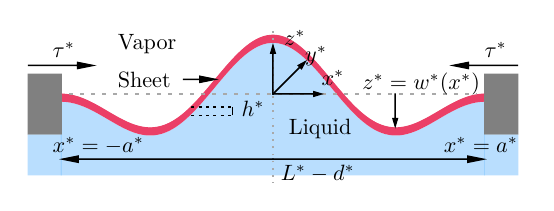
\begin{tikzpicture}

\definecolor{darkgray}{RGB}{169,169,169}
\definecolor{darkgray176}{RGB}{176,176,176}
\definecolor{gray}{RGB}{128,128,128}
\definecolor{indianred23563103}{RGB}{235,63,103}
\definecolor{lightskyblue138200253}{RGB}{138,200,253}

\begin{axis}[
axis equal image,
hide x axis,
hide y axis,
tick align=outside,
tick pos=left,
x grid style={darkgray176},
xlabel={0},
xmin=-0.03311, xmax=0.03311,
xtick style={color=black},
y grid style={darkgray176},
ymin=-0.010863663529839, ymax=0.00813693412661942,
ytick style={color=black}
]
\path [fill=lightskyblue138200253, fill opacity=0.6]
(axis cs:-0.0260467875630729,-0.00095)
--(axis cs:-0.0260467875630729,-0.00095)
--(axis cs:-0.0259887601975588,-0.000950265193764294)
--(axis cs:-0.0259307328320446,-0.000951060839657842)
--(axis cs:-0.0258727054665305,-0.000952386935837379)
--(axis cs:-0.0258146781010164,-0.000954243348798273)
--(axis cs:-0.0257566507355023,-0.000956629813394401)
--(axis cs:-0.0256986233699882,-0.000959545932885385)
--(axis cs:-0.0256405960044741,-0.0009629911790112)
--(axis cs:-0.02558256863896,-0.0009669648920941)
--(axis cs:-0.0255245412734459,-0.0009714662811679)
--(axis cs:-0.0254665139079318,-0.0009764944241347)
--(axis cs:-0.0254084865424177,-0.0009820482679484)
--(axis cs:-0.0253504591769036,-0.0009881266288259)
--(axis cs:-0.0252924318113895,-0.0009947281924857)
--(axis cs:-0.0252344044458754,-0.0010018515144127)
--(axis cs:-0.0251763770803613,-0.0010094950201512)
--(axis cs:-0.0251183497148472,-0.0010176570056243)
--(axis cs:-0.0250603223493331,-0.00102633563748)
--(axis cs:-0.025002294983819,-0.0010355289534653)
--(axis cs:-0.0249442676183049,-0.001045234862826)
--(axis cs:-0.0248862402527908,-0.0010554511467335)
--(axis cs:-0.0248282128872767,-0.0010661754587388)
--(axis cs:-0.0247701855217626,-0.0010774053252526)
--(axis cs:-0.0247121581562485,-0.0010891381460517)
--(axis cs:-0.0246541307907344,-0.0011013711948125)
--(axis cs:-0.0245961034252203,-0.00111410161967)
--(axis cs:-0.0245380760597062,-0.0011273264438032)
--(axis cs:-0.0244800486941921,-0.0011410425660469)
--(axis cs:-0.024422021328678,-0.001155246761529)
--(axis cs:-0.0243639939631638,-0.0011699356823334)
--(axis cs:-0.0243059665976497,-0.0011851058581895)
--(axis cs:-0.0242479392321356,-0.0012007536971861)
--(axis cs:-0.0241899118666215,-0.0012168754865111)
--(axis cs:-0.0241318845011074,-0.0012334673932171)
--(axis cs:-0.0240738571355933,-0.0012505254650108)
--(axis cs:-0.0240158297700792,-0.0012680456310682)
--(axis cs:-0.0239578024045651,-0.0012860237028747)
--(axis cs:-0.023899775039051,-0.0013044553750889)
--(axis cs:-0.0238417476735369,-0.0013233362264317)
--(axis cs:-0.0237837203080228,-0.0013426617205992)
--(axis cs:-0.0237256929425087,-0.0013624272071996)
--(axis cs:-0.0236676655769946,-0.0013826279227144)
--(axis cs:-0.0236096382114805,-0.0014032589914829)
--(axis cs:-0.0235516108459664,-0.00142431542671)
--(axis cs:-0.0234935834804523,-0.0014457921314979)
--(axis cs:-0.0234355561149382,-0.0014676838999004)
--(axis cs:-0.0233775287494241,-0.0014899854180001)
--(axis cs:-0.02331950138391,-0.0015126912650084)
--(axis cs:-0.0232614740183959,-0.001535795914388)
--(axis cs:-0.0232034466528818,-0.0015592937349971)
--(axis cs:-0.0231454192873677,-0.0015831789922564)
--(axis cs:-0.0230873919218536,-0.0016074458493369)
--(axis cs:-0.0230293645563395,-0.0016320883683701)
--(axis cs:-0.0229713371908254,-0.0016571005116786)
--(axis cs:-0.0229133098253113,-0.0016824761430286)
--(axis cs:-0.0228552824597972,-0.0017082090289024)
--(axis cs:-0.022797255094283,-0.0017342928397919)
--(axis cs:-0.0227392277287689,-0.0017607211515122)
--(axis cs:-0.0226812003632548,-0.0017874874465348)
--(axis cs:-0.0226231729977407,-0.0018145851153413)
--(axis cs:-0.0225651456322266,-0.0018420074577962)
--(axis cs:-0.0225071182667125,-0.0018697476845382)
--(axis cs:-0.0224490909011984,-0.0018977989183919)
--(axis cs:-0.0223910635356843,-0.0019261541957963)
--(axis cs:-0.0223330361701702,-0.0019548064682534)
--(axis cs:-0.0222750088046561,-0.0019837486037933)
--(axis cs:-0.022216981439142,-0.0020129733884583)
--(axis cs:-0.0221589540736279,-0.0020424735278035)
--(axis cs:-0.0221009267081138,-0.0020722416484151)
--(axis cs:-0.0220428993425997,-0.0021022702994453)
--(axis cs:-0.0219848719770856,-0.0021325519541642)
--(axis cs:-0.0219268446115715,-0.0021630790115269)
--(axis cs:-0.0218688172460574,-0.0021938437977579)
--(axis cs:-0.0218107898805433,-0.0022248385679495)
--(axis cs:-0.0217527625150292,-0.0022560555076774)
--(axis cs:-0.0216947351495151,-0.0022874867346291)
--(axis cs:-0.021636707784001,-0.002319124300249)
--(axis cs:-0.0215786804184869,-0.0023509601913962)
--(axis cs:-0.0215206530529728,-0.0023829863320169)
--(axis cs:-0.0214626256874587,-0.0024151945848308)
--(axis cs:-0.0214045983219446,-0.0024475767530302)
--(axis cs:-0.0213465709564305,-0.002480124581992)
--(axis cs:-0.0212885435909164,-0.0025128297610032)
--(axis cs:-0.0212305162254023,-0.0025456839249973)
--(axis cs:-0.0211724888598882,-0.002578678656304)
--(axis cs:-0.021114461494374,-0.0026118054864094)
--(axis cs:-0.0210564341288599,-0.0026450558977279)
--(axis cs:-0.0209984067633458,-0.0026784213253852)
--(axis cs:-0.0209403793978317,-0.002711893159011)
--(axis cs:-0.0208823520323176,-0.0027454627445428)
--(axis cs:-0.0208243246668035,-0.0027791213860387)
--(axis cs:-0.0207662973012894,-0.0028128603475)
--(axis cs:-0.0207082699357753,-0.0028466708547028)
--(axis cs:-0.0206502425702612,-0.0028805440970383)
--(axis cs:-0.0205922152047471,-0.0029144712293615)
--(axis cs:-0.020534187839233,-0.0029484433738474)
--(axis cs:-0.0204761604737189,-0.0029824516218552)
--(axis cs:-0.0204181331082048,-0.0030164870357999)
--(axis cs:-0.0203601057426907,-0.0030505406510301)
--(axis cs:-0.0203020783771766,-0.0030846034777124)
--(axis cs:-0.0202440510116625,-0.0031186665027225)
--(axis cs:-0.0201860236461484,-0.0031527206915414)
--(axis cs:-0.0201279962806343,-0.0031867569901566)
--(axis cs:-0.0200699689151202,-0.0032207663269691)
--(axis cs:-0.0200119415496061,-0.0032547396147045)
--(axis cs:-0.019953914184092,-0.0032886677523278)
--(axis cs:-0.0198958868185779,-0.0033225416269632)
--(axis cs:-0.0198378594530638,-0.0033563521158155)
--(axis cs:-0.0197798320875497,-0.0033900900880965)
--(axis cs:-0.0197218047220356,-0.0034237464069524)
--(axis cs:-0.0196637773565215,-0.0034573119313946)
--(axis cs:-0.0196057499910074,-0.0034907775182313)
--(axis cs:-0.0195477226254933,-0.0035241340240011)
--(axis cs:-0.0194896952599792,-0.0035573723069084)
--(axis cs:-0.019431667894465,-0.0035904832287575)
--(axis cs:-0.0193736405289509,-0.0036234576568893)
--(axis cs:-0.0193156131634368,-0.0036562864661163)
--(axis cs:-0.0192575857979227,-0.0036889605406574)
--(axis cs:-0.0191995584324086,-0.0037214707760725)
--(axis cs:-0.0191415310668945,-0.0037538080811952)
--(axis cs:-0.0190835037013804,-0.003785963380064)
--(axis cs:-0.0190254763358663,-0.0038179276138512)
--(axis cs:-0.0189674489703522,-0.0038496917427901)
--(axis cs:-0.0189094216048381,-0.0038812467480988)
--(axis cs:-0.018851394239324,-0.0039125836339006)
--(axis cs:-0.0187933668738099,-0.0039436934291412)
--(axis cs:-0.0187353395082958,-0.0039745671895024)
--(axis cs:-0.0186773121427817,-0.0040051959993101)
--(axis cs:-0.0186192847772676,-0.0040355709734386)
--(axis cs:-0.0185612574117535,-0.0040656832592097)
--(axis cs:-0.0185032300462394,-0.0040955240382859)
--(axis cs:-0.0184452026807253,-0.0041250845285578)
--(axis cs:-0.0183871753152112,-0.0041543559860256)
--(axis cs:-0.0183291479496971,-0.004183329706673)
--(axis cs:-0.018271120584183,-0.0042119970283357)
--(axis cs:-0.0182130932186689,-0.0042403493325605)
--(axis cs:-0.0181550658531548,-0.0042683780464584)
--(axis cs:-0.0180970384876407,-0.0042960746445482)
--(axis cs:-0.0180390111221266,-0.0043234306505924)
--(axis cs:-0.0179809837566125,-0.0043504376394242)
--(axis cs:-0.0179229563910984,-0.0043770872387641)
--(axis cs:-0.0178649290255843,-0.0044033711310288)
--(axis cs:-0.0178069016600702,-0.0044292810551283)
--(axis cs:-0.0177488742945561,-0.0044548088082534)
--(axis cs:-0.0176908469290419,-0.0044799462476529)
--(axis cs:-0.0176328195635278,-0.0045046852923988)
--(axis cs:-0.0175747921980137,-0.0045290179251406)
--(axis cs:-0.0175167648324996,-0.0045529361938479)
--(axis cs:-0.0174587374669855,-0.0045764322135405)
--(axis cs:-0.0174007101014714,-0.0045994981680062)
--(axis cs:-0.0173426827359573,-0.0046221263115058)
--(axis cs:-0.0172846553704432,-0.0046443089704646)
--(axis cs:-0.0172266280049291,-0.004666038545151)
--(axis cs:-0.017168600639415,-0.0046873075113404)
--(axis cs:-0.0171105732739009,-0.0047081084219658)
--(axis cs:-0.0170525459083868,-0.0047284339087529)
--(axis cs:-0.0169945185428727,-0.004748276683841)
--(axis cs:-0.0169364911773586,-0.0047676295413887)
--(axis cs:-0.0168784638118445,-0.0047864853591634)
--(axis cs:-0.0168204364463304,-0.004804837100116)
--(axis cs:-0.0167624090808163,-0.0048226778139384)
--(axis cs:-0.0167043817153022,-0.0048400006386051)
--(axis cs:-0.0166463543497881,-0.004856798801898)
--(axis cs:-0.016588326984274,-0.0048730656229136)
--(axis cs:-0.0165302996187599,-0.0048887945135536)
--(axis cs:-0.0164722722532458,-0.0049039789799969)
--(axis cs:-0.0164142448877317,-0.0049186126241543)
--(axis cs:-0.0163562175222176,-0.0049326891451044)
--(axis cs:-0.0162981901567035,-0.004946202340511)
--(axis cs:-0.0162401627911894,-0.0049591461080219)
--(axis cs:-0.0161821354256753,-0.0049715144466483)
--(axis cs:-0.0161241080601612,-0.0049833014581245)
--(axis cs:-0.016066080694647,-0.0049945013482481)
--(axis cs:-0.0160080533291329,-0.0050051084282006)
--(axis cs:-0.0159500259636188,-0.0050151171158466)
--(axis cs:-0.0158919985981047,-0.0050245219370138)
--(axis cs:-0.0158339712325906,-0.0050333175267513)
--(axis cs:-0.0157759438670765,-0.0050414986305666)
--(axis cs:-0.0157179165015624,-0.0050490601056428)
--(axis cs:-0.0156598891360483,-0.0050559969220319)
--(axis cs:-0.0156018617705342,-0.0050623041638287)
--(axis cs:-0.0155438344050201,-0.0050679770303207)
--(axis cs:-0.015485807039506,-0.0050730108371168)
--(axis cs:-0.0154277796739919,-0.0050774010172532)
--(axis cs:-0.0153697523084778,-0.0050811431222766)
--(axis cs:-0.0153117249429637,-0.005084232823304)
--(axis cs:-0.0152536975774496,-0.0050866659120601)
--(axis cs:-0.0151956702119355,-0.0050884383018905)
--(axis cs:-0.0151376428464214,-0.0050895460287518)
--(axis cs:-0.0150796154809073,-0.0050899852521776)
--(axis cs:-0.0150215881153932,-0.0050897522562207)
--(axis cs:-0.0149635607498791,-0.0050888434503707)
--(axis cs:-0.014905533384365,-0.005087255370448)
--(axis cs:-0.0148475060188509,-0.0050849846794718)
--(axis cs:-0.0147894786533368,-0.0050820281685051)
--(axis cs:-0.0147314512878227,-0.005078382757473)
--(axis cs:-0.0146734239223086,-0.0050740454959573)
--(axis cs:-0.0146153965567945,-0.005069013563965)
--(axis cs:-0.0145573691912804,-0.0050632842726713)
--(axis cs:-0.0144993418257662,-0.0050568550651379)
--(axis cs:-0.0144413144602522,-0.0050497235170041)
--(axis cs:-0.014383287094738,-0.0050418873371532)
--(axis cs:-0.0143252597292239,-0.0050333443683527)
--(axis cs:-0.0142672323637098,-0.0050240925878675)
--(axis cs:-0.0142092049981957,-0.0050141301080476)
--(axis cs:-0.0141511776326816,-0.0050034551768892)
--(axis cs:-0.0140931502671675,-0.0049920661785691)
--(axis cs:-0.0140351229016534,-0.0049799616339523)
--(axis cs:-0.0139770955361393,-0.0049671402010732)
--(axis cs:-0.0139190681706252,-0.0049536006755896)
--(axis cs:-0.0138610408051111,-0.0049393419912099)
--(axis cs:-0.013803013439597,-0.0049243632200929)
--(axis cs:-0.0137449860740829,-0.004908663573221)
--(axis cs:-0.0136869587085688,-0.0048922424007455)
--(axis cs:-0.0136289313430547,-0.0048750991923051)
--(axis cs:-0.0135709039775406,-0.0048572335773168)
--(axis cs:-0.0135128766120265,-0.0048386453252388)
--(axis cs:-0.0134548492465124,-0.0048193343458073)
--(axis cs:-0.0133968218809983,-0.0047993006892437)
--(axis cs:-0.0133387945154842,-0.0047785445464361)
--(axis cs:-0.0132807671499701,-0.004757066249092)
--(axis cs:-0.013222739784456,-0.0047348662698632)
--(axis cs:-0.0131647124189419,-0.0047119452224437)
--(axis cs:-0.0131066850534278,-0.0046883038616392)
--(axis cs:-0.0130486576879137,-0.0046639430834091)
--(axis cs:-0.0129906303223996,-0.0046388639248803)
--(axis cs:-0.0129326029568855,-0.0046130675643335)
--(axis cs:-0.0128745755913714,-0.0045865553211618)
--(axis cs:-0.0128165482258572,-0.0045593286558008)
--(axis cs:-0.0127585208603431,-0.0045313891696316)
--(axis cs:-0.012700493494829,-0.0045027386048555)
--(axis cs:-0.0126424661293149,-0.0044733788443407)
--(axis cs:-0.0125844387638008,-0.0044433119114421)
--(axis cs:-0.0125264113982867,-0.0044125399697922)
--(axis cs:-0.0124683840327726,-0.004381065323065)
--(axis cs:-0.0124103566672585,-0.0043488904147121)
--(axis cs:-0.0123523293017444,-0.0043160178276705)
--(axis cs:-0.0122943019362303,-0.0042824502840439)
--(axis cs:-0.0122362745707162,-0.0042481906447556)
--(axis cs:-0.0121782472052021,-0.0042132419091739)
--(axis cs:-0.012120219839688,-0.0041776072147107)
--(axis cs:-0.0120621924741739,-0.0041412898363918)
--(axis cs:-0.0120041651086598,-0.0041042931864011)
--(axis cs:-0.0119461377431457,-0.0040666208135963)
--(axis cs:-0.0118881103776316,-0.0040282764029982)
--(axis cs:-0.0118300830121175,-0.0039892637752531)
--(axis cs:-0.0117720556466034,-0.0039495868860678)
--(axis cs:-0.0117140282810893,-0.0039092498256181)
--(axis cs:-0.0116560009155752,-0.0038682568179303)
--(axis cs:-0.0115979735500611,-0.0038266122202361)
--(axis cs:-0.011539946184547,-0.0037843205223014)
--(axis cs:-0.0114819188190329,-0.0037413863457285)
--(axis cs:-0.0114238914535188,-0.0036978144432314)
--(axis cs:-0.0113658640880047,-0.0036536096978864)
--(axis cs:-0.0113078367224906,-0.003608777122355)
--(axis cs:-0.0112498093569765,-0.0035633218580827)
--(axis cs:-0.0111917819914624,-0.0035172491744708)
--(axis cs:-0.0111337546259482,-0.0034705644680232)
--(axis cs:-0.0110757272604341,-0.0034232732614678)
--(axis cs:-0.01101769989492,-0.0033753812028528)
--(axis cs:-0.0109596725294059,-0.0033268940646176)
--(axis cs:-0.0109016451638918,-0.0032778177426395)
--(axis cs:-0.0108436177983777,-0.0032281582552545)
--(axis cs:-0.0107855904328636,-0.0031779217422552)
--(axis cs:-0.0107275630673495,-0.0031271144638632)
--(axis cs:-0.0106695357018354,-0.0030757427996777)
--(axis cs:-0.0106115083363213,-0.0030238132476002)
--(axis cs:-0.0105534809708072,-0.002971332422736)
--(axis cs:-0.0104954536052931,-0.0029183070562708)
--(axis cs:-0.010437426239779,-0.0028647439943259)
--(axis cs:-0.0103793988742649,-0.0028106501967886)
--(axis cs:-0.0103213715087508,-0.0027560327361208)
--(axis cs:-0.0102633441432367,-0.0027008987961445)
--(axis cs:-0.0102053167777226,-0.0026452556708052)
--(axis cs:-0.0101472894122085,-0.0025891107629128)
--(axis cs:-0.0100892620466944,-0.0025324715828607)
--(axis cs:-0.0100312346811803,-0.0024753457473236)
--(axis cs:-0.0099732073156662,-0.002417740977933)
--(axis cs:-0.0099151799501521,-0.0023596650999325)
--(axis cs:-0.009857152584638,-0.0023011260408115)
--(axis cs:-0.0097991252191239,-0.0022421318289185)
--(axis cs:-0.0097410978536098,-0.0021826905920538)
--(axis cs:-0.0096830704880957,-0.0021228105560424)
--(axis cs:-0.0096250431225816,-0.002062500043287)
--(axis cs:-0.0095670157570675,-0.0020017674713008)
--(axis cs:-0.0095089883915534,-0.001940621351222)
--(axis cs:-0.0094509610260392,-0.0018790702863083)
--(axis cs:-0.0093929336605251,-0.0018171229704134)
--(axis cs:-0.009334906295011,-0.001754788186445)
--(axis cs:-0.0092768789294969,-0.0016920748048038)
--(axis cs:-0.0092188515639828,-0.0016289917818061)
--(axis cs:-0.0091608241984687,-0.0015655481580875)
--(axis cs:-0.0091027968329546,-0.0015017530569903)
--(axis cs:-0.0090447694674405,-0.0014376156829333)
--(axis cs:-0.0089867421019264,-0.0013731453197656)
--(axis cs:-0.0089287147364123,-0.0013083513291039)
--(axis cs:-0.0088706873708982,-0.0012432431486535)
--(axis cs:-0.0088126600053841,-0.0011778302905138)
--(axis cs:-0.00875463263987,-0.0011121223394691)
--(axis cs:-0.0086966052743559,-0.0010461289512635)
--(axis cs:-0.0086385779088418,-0.0009798598508618)
--(axis cs:-0.0085805505433277,-0.0009133248306954)
--(axis cs:-0.0085225231778136,-0.0008465337488949)
--(axis cs:-0.0084644958122995,-0.000779496527509)
--(axis cs:-0.0084064684467854,-0.0007122231507094)
--(axis cs:-0.0083484410812713,-0.0006447236629836)
--(axis cs:-0.0082904137157572,-0.0005770081673146)
--(axis cs:-0.0082323863502431,-0.0005090868233482)
--(axis cs:-0.008174358984729,-0.000440969845549)
--(axis cs:-0.0081163316192149,-0.0003726675013445)
--(axis cs:-0.0080583042537008,-0.0003041901092578)
--(axis cs:-0.0080002768881867,-0.0002355480370296)
--(axis cs:-0.0079422495226726,-0.0001667516997302)
--(axis cs:-0.0078842221571585,-9.78115578609e-05)
--(axis cs:-0.0078261947916443,-2.87381154455e-05)
--(axis cs:-0.0077681674261302,4.04580818869001e-05)
--(axis cs:-0.0077101400606161,0.0001097664488288)
--(axis cs:-0.007652112695102,0.000179176362329)
--(axis cs:-0.0075940853295879,0.0002486771635367)
--(axis cs:-0.0075360579640738,0.0003182581597521)
--(axis cs:-0.0074780305985597,0.0003879086263859)
--(axis cs:-0.0074200032330456,0.0004576178089245)
--(axis cs:-0.0073619758675315,0.0005273749249031)
--(axis cs:-0.0073039485020174,0.0005971691658846)
--(axis cs:-0.0072459211365033,0.0006669896994445)
--(axis cs:-0.0071878937709892,0.0007368256711616)
--(axis cs:-0.0071298664054751,0.0008066662066133)
--(axis cs:-0.007071839039961,0.0008765004133766)
--(axis cs:-0.0070138116744469,0.000946317383033)
--(axis cs:-0.0069557843089328,0.0010161061931771)
--(axis cs:-0.0068977569434187,0.0010858559094298)
--(axis cs:-0.0068397295779046,0.0011555555874539)
--(axis cs:-0.0067817022123905,0.0012251942749728)
--(axis cs:-0.0067236748468764,0.0012947610137919)
--(axis cs:-0.0066656474813623,0.0013642448418217)
--(axis cs:-0.0066076201158482,0.001433634795103)
--(axis cs:-0.0065495927503341,0.0015029199098332)
--(axis cs:-0.00649156538482,0.0015720892243932)
--(axis cs:-0.0064335380193059,0.0016411317813754)
--(axis cs:-0.0063755106537918,0.0017100366296114)
--(axis cs:-0.0063174832882777,0.0017787928261994)
--(axis cs:-0.0062594559227636,0.0018473894385313)
--(axis cs:-0.0062014285572495,0.0019158155463182)
--(axis cs:-0.0061434011917353,0.0019840602436151)
--(axis cs:-0.0060853738262212,0.0020521126408427)
--(axis cs:-0.0060273464607071,0.0021199618668086)
--(axis cs:-0.005969319095193,0.0021875970707238)
--(axis cs:-0.0059112917296789,0.002255007424218)
--(axis cs:-0.0058532643641648,0.0023221821233506)
--(axis cs:-0.0057952369986507,0.0023891103906177)
--(axis cs:-0.0057372096331366,0.0024557814769555)
--(axis cs:-0.0056791822676225,0.0025221846637386)
--(axis cs:-0.0056211549021084,0.0025883092647736)
--(axis cs:-0.0055631275365943,0.0026541446282875)
--(axis cs:-0.0055051001710802,0.0027196801389097)
--(axis cs:-0.0054470728055661,0.0027849052196483)
--(axis cs:-0.005389045440052,0.0028498093338603)
--(axis cs:-0.0053310180745379,0.0029143819872138)
--(axis cs:-0.0052729907090238,0.0029786127296439)
--(axis cs:-0.0052149633435097,0.0030424911573005)
--(axis cs:-0.0051569359779956,0.0031060069144879)
--(axis cs:-0.0050989086124815,0.0031691496955965)
--(axis cs:-0.0050408812469674,0.0032319092470251)
--(axis cs:-0.0049828538814533,0.0032942753690946)
--(axis cs:-0.0049248265159392,0.0033562379179513)
--(axis cs:-0.0048667991504251,0.0034177868074615)
--(axis cs:-0.004808771784911,0.0034789120110947)
--(axis cs:-0.0047507444193969,0.0035396035637965)
--(axis cs:-0.0046927170538828,0.003599851563851)
--(axis cs:-0.0046346896883687,0.0036596461747309)
--(axis cs:-0.0045766623228546,0.0037189776269367)
--(axis cs:-0.0045186349573404,0.0037778362198231)
--(axis cs:-0.0044606075918263,0.0038362123234136)
--(axis cs:-0.0044025802263122,0.0038940963802016)
--(axis cs:-0.0043445528607981,0.003951478906939)
--(axis cs:-0.004286525495284,0.0040083504964109)
--(axis cs:-0.0042284981297699,0.0040647018191964)
--(axis cs:-0.0041704707642558,0.0041205236254156)
--(axis cs:-0.0041124433987417,0.0041758067464615)
--(axis cs:-0.0040544160332276,0.0042305420967175)
--(axis cs:-0.0039963886677135,0.0042847206752595)
--(axis cs:-0.0039383613021994,0.0043383335675425)
--(axis cs:-0.0038803339366853,0.0043913719470711)
--(axis cs:-0.0038223065711712,0.0044438270770541)
--(axis cs:-0.0037642792056571,0.0044956903120428)
--(axis cs:-0.003706251840143,0.0045469530995516)
--(axis cs:-0.0036482244746289,0.0045976069816624)
--(axis cs:-0.0035901971091148,0.0046476435966109)
--(axis cs:-0.0035321697436007,0.0046970546803555)
--(axis cs:-0.0034741423780866,0.0047458320681279)
--(axis cs:-0.0034161150125725,0.0047939676959654)
--(axis cs:-0.0033580876470584,0.0048414536022244)
--(axis cs:-0.0033000602815443,0.0048882819290753)
--(axis cs:-0.0032420329160302,0.0049344449239776)
--(axis cs:-0.0031840055505161,0.0049799349411358)
--(axis cs:-0.003125978185002,0.0050247444429354)
--(axis cs:-0.0030679508194879,0.0050688660013585)
--(axis cs:-0.0030099234539738,0.0051122922993799)
--(axis cs:-0.0029518960884597,0.0051550161323409)
--(axis cs:-0.0028938687229456,0.0051970304093041)
--(axis cs:-0.0028358413574314,0.0052383281543854)
--(axis cs:-0.0027778139919173,0.0052789025080655)
--(axis cs:-0.0027197866264032,0.0053187467284794)
--(axis cs:-0.0026617592608891,0.0053578541926837)
--(axis cs:-0.002603731895375,0.0053962183979018)
--(axis cs:-0.0025457045298609,0.0054338329627473)
--(axis cs:-0.0024876771643468,0.0054706916284235)
--(axis cs:-0.0024296497988327,0.0055067882599011)
--(axis cs:-0.0023716224333186,0.0055421168470718)
--(axis cs:-0.0023135950678045,0.0055766715058794)
--(axis cs:-0.0022555677022904,0.0056104464794266)
--(axis cs:-0.0021975403367763,0.0056434361390583)
--(axis cs:-0.0021395129712622,0.0056756349854209)
--(axis cs:-0.0020814856057481,0.0057070376494972)
--(axis cs:-0.002023458240234,0.0057376388936169)
--(axis cs:-0.0019654308747199,0.0057674336124427)
--(axis cs:-0.0019074035092058,0.005796416833931)
--(axis cs:-0.0018493761436917,0.0058245837202684)
--(axis cs:-0.0017913487781776,0.0058519295687821)
--(axis cs:-0.0017333214126635,0.0058784498128259)
--(axis cs:-0.0016752940471494,0.0059041400226397)
--(axis cs:-0.0016172666816353,0.0059289959061837)
--(axis cs:-0.0015592393161212,0.0059530133099471)
--(axis cs:-0.0015012119506071,0.0059761882197301)
--(axis cs:-0.001443184585093,0.0059985167614001)
--(axis cs:-0.0013851572195789,0.0060199952016214)
--(axis cs:-0.0013271298540648,0.0060406199485585)
--(axis cs:-0.0012691024885507,0.006060387552553)
--(axis cs:-0.0012110751230365,0.0060792947067731)
--(axis cs:-0.0011530477575224,0.0060973382478368)
--(axis cs:-0.0010950203920083,0.0061145151564082)
--(axis cs:-0.0010369930264942,0.0061308225577661)
--(axis cs:-0.0009789656609801,0.0061462577223458)
--(axis cs:-0.000920938295466,0.0061608180662536)
--(axis cs:-0.0008629109299519,0.0061745011517535)
--(axis cs:-0.0008048835644378,0.0061873046877267)
--(axis cs:-0.0007468561989237,0.0061992265301038)
--(axis cs:-0.0006888288334096,0.0062102646822681)
--(axis cs:-0.0006308014678955,0.0062204172954327)
--(axis cs:-0.0005727741023814,0.0062296826689883)
--(axis cs:-0.0005147467368673,0.0062380592508244)
--(axis cs:-0.0004567193713532,0.0062455456376213)
--(axis cs:-0.0003986920058391,0.0062521405751149)
--(axis cs:-0.000340664640325,0.0062578429583332)
--(axis cs:-0.0002826372748109,0.0062626518318042)
--(axis cs:-0.0002246099092968,0.0062665663897367)
--(axis cs:-0.0001665825437827,0.0062695859761714)
--(axis cs:-0.0001085551782686,0.0062717100851051)
--(axis cs:-5.05278127545e-05,0.0062729383605859)
--(axis cs:7.49955275957484e-06,0.0062732705967804)
--(axis cs:6.55269182736e-05,0.0062727067380123)
--(axis cs:0.0001235542837877,0.0062712468787732)
--(axis cs:0.0001815816493018,0.0062688912637045)
--(axis cs:0.0002396090148159,0.0062656402875514)
--(axis cs:0.00029763638033,0.0062614944950884)
--(axis cs:0.0003556637458441,0.006256454581017)
--(axis cs:0.0004136911113583,0.006250521389834)
--(axis cs:0.0004717184768724,0.0062436959156731)
--(axis cs:0.0005297458423865,0.0062359793021168)
--(axis cs:0.0005877732079006,0.0062273728419815)
--(axis cs:0.0006458005734147,0.0062178779770732)
--(axis cs:0.0007038279389288,0.0062074962979162)
--(axis cs:0.0007618553044429,0.0061962295434529)
--(axis cs:0.000819882669957,0.0061840796007164)
--(axis cs:0.0008779100354711,0.0061710485044744)
--(axis cs:0.0009359374009852,0.0061571384368463)
--(axis cs:0.0009939647664993,0.0061423517268912)
--(axis cs:0.0010519921320134,0.0061266908501698)
--(axis cs:0.0011100194975275,0.0061101584282769)
--(axis cs:0.0011680468630416,0.0060927572283482)
--(axis cs:0.0012260742285557,0.0060744901625383)
--(axis cs:0.0012841015940698,0.0060553602874725)
--(axis cs:0.0013421289595839,0.0060353708036701)
--(axis cs:0.001400156325098,0.0060145250549421)
--(axis cs:0.0014581836906121,0.0059928265277606)
--(axis cs:0.0015162110561262,0.0059702788506027)
--(axis cs:0.0015742384216403,0.0059468857932659)
--(axis cs:0.0016322657871544,0.005922651266159)
--(axis cs:0.0016902931526685,0.0058975793195649)
--(axis cs:0.0017483205181826,0.0058716741428779)
--(axis cs:0.0018063478836967,0.0058449400638145)
--(axis cs:0.0018643752492108,0.0058173815475987)
--(axis cs:0.0019224026147249,0.0057890031961207)
--(axis cs:0.001980429980239,0.0057598097470708)
--(axis cs:0.0020384573457531,0.005729806073047)
--(axis cs:0.0020964847112673,0.0056989971806378)
--(axis cs:0.0021545120767814,0.0056673882094794)
--(axis cs:0.0022125394422955,0.0056349844312886)
--(axis cs:0.0022705668078096,0.0056017912488703)
--(axis cs:0.0023285941733237,0.0055678141951005)
--(axis cs:0.0023866215388378,0.0055330589318852)
--(axis cs:0.0024446489043519,0.0054975312490949)
--(axis cs:0.002502676269866,0.0054612370634753)
--(axis cs:0.0025607036353801,0.005424182417534)
--(axis cs:0.0026187310008942,0.0053863734784036)
--(axis cs:0.0026767583664083,0.0053478165366819)
--(axis cs:0.0027347857319224,0.0053085180052486)
--(axis cs:0.0027928130974365,0.0052684844180596)
--(axis cs:0.0028508404629506,0.0052277224289176)
--(axis cs:0.0029088678284647,0.0051862388102218)
--(axis cs:0.0029668951939788,0.0051440404516942)
--(axis cs:0.0030249225594929,0.0051011343590849)
--(axis cs:0.003082949925007,0.0050575276528549)
--(axis cs:0.0031409772905211,0.0050132275668382)
--(axis cs:0.0031990046560352,0.0049682414468826)
--(axis cs:0.0032570320215493,0.0049225767494693)
--(axis cs:0.0033150593870634,0.0048762410403122)
--(axis cs:0.0033730867525775,0.0048292419929372)
--(axis cs:0.0034311141180916,0.0047815873872405)
--(axis cs:0.0034891414836057,0.004733285108028)
--(axis cs:0.0035471688491198,0.0046843431435352)
--(axis cs:0.0036051962146339,0.0046347695839272)
--(axis cs:0.003663223580148,0.0045845726197802)
--(axis cs:0.0037212509456621,0.004533760540545)
--(axis cs:0.0037792783111762,0.004482341732991)
--(axis cs:0.0038373056766904,0.0044303246796332)
--(axis cs:0.0038953330422045,0.0043777179571411)
--(axis cs:0.0039533604077186,0.0043245302347299)
--(axis cs:0.0040113877732327,0.0042707702725355)
--(axis cs:0.0040694151387468,0.0042164469199718)
--(axis cs:0.0041274425042609,0.0041615691140721)
--(axis cs:0.004185469869775,0.0041061458778145)
--(axis cs:0.0042434972352891,0.0040501863184309)
--(axis cs:0.0043015246008032,0.0039936996257012)
--(axis cs:0.0043595519663173,0.0039366950702318)
--(axis cs:0.0044175793318314,0.0038791820017202)
--(axis cs:0.0044756066973455,0.0038211698472038)
--(axis cs:0.0045336340628596,0.003762668109296)
--(axis cs:0.0045916614283737,0.0037036863644075)
--(axis cs:0.0046496887938878,0.0036442342609547)
--(axis cs:0.0047077161594019,0.0035843215175549)
--(axis cs:0.004765743524916,0.0035239579212088)
--(axis cs:0.0048237708904301,0.0034631533254706)
--(axis cs:0.0048817982559442,0.0034019176486059)
--(axis cs:0.0049398256214583,0.0033402608717384)
--(axis cs:0.0049978529869724,0.0032781930369852)
--(axis cs:0.0050558803524865,0.0032157242455805)
--(axis cs:0.0051139077180006,0.0031528646559898)
--(axis cs:0.0051719350835147,0.003089624482013)
--(axis cs:0.0052299624490288,0.0030260139908785)
--(axis cs:0.0052879898145429,0.0029620435013268)
--(axis cs:0.005346017180057,0.0028977233816861)
--(axis cs:0.0054040445455711,0.0028330640479385)
--(axis cs:0.0054620719110853,0.0027680759617783)
--(axis cs:0.0055200992765994,0.0027027696286617)
--(axis cs:0.0055781266421135,0.0026371555958498)
--(axis cs:0.0056361540076276,0.0025712444504435)
--(axis cs:0.0056941813731417,0.0025050468174126)
--(axis cs:0.0057522087386558,0.0024385733576175)
--(axis cs:0.0058102361041699,0.0023718347658253)
--(axis cs:0.005868263469684,0.0023048417687207)
--(axis cs:0.0059262908351981,0.0022376051229103)
--(axis cs:0.0059843182007122,0.0021701356129237)
--(axis cs:0.0060423455662263,0.0021024440492087)
--(axis cs:0.0061003729317404,0.0020345412661233)
--(axis cs:0.0061584002972545,0.0019664381199237)
--(axis cs:0.0062164276627686,0.0018981454867484)
--(axis cs:0.0062744550282827,0.0018296742606007)
--(axis cs:0.0063324823937968,0.0017610353513271)
--(axis cs:0.0063905097593109,0.001692239682595)
--(axis cs:0.006448537124825,0.0016232981898673)
--(axis cs:0.0065065644903391,0.001554221818377)
--(axis cs:0.0065645918558532,0.0014850215210994)
--(axis cs:0.0066226192213673,0.0014157082567252)
--(axis cs:0.0066806465868814,0.001346292987632)
--(axis cs:0.0067386739523955,0.0012767866778573)
--(axis cs:0.0067967013179096,0.0012072002910712)
--(axis cs:0.0068547286834237,0.0011375447885503)
--(axis cs:0.0069127560489378,0.0010678311271533)
--(axis cs:0.0069707834144519,0.0009980702572983)
--(axis cs:0.007028810779966,0.0009282731209418)
--(axis cs:0.0070868381454802,0.0008584506495611)
--(axis cs:0.0071448655109943,0.0007886137621388)
--(axis cs:0.0072028928765084,0.0007187733631513)
--(axis cs:0.0072609202420225,0.0006489403405607)
--(axis cs:0.0073189476075366,0.0005791255638111)
--(axis cs:0.0073769749730507,0.000509339881829)
--(axis cs:0.0074350023385648,0.0004395941210292)
--(axis cs:0.0074930297040789,0.0003698990833254)
--(axis cs:0.007551057069593,0.0003002655441467)
--(axis cs:0.0076090844351071,0.0002307042504607)
--(axis cs:0.0076671118006212,0.0001612259188018)
--(axis cs:0.0077251391661353,9.1841233308e-05)
--(axis cs:0.0077831665316494,2.2560843763e-05)
--(axis cs:0.0078411938971635,-4.6604636352e-05)
--(axis cs:0.0078992212626776,-0.0001156446318008)
--(axis cs:0.0079572486281917,-0.0001845486075241)
--(axis cs:0.0080152759937058,-0.0002533060705646)
--(axis cs:0.0080733033592199,-0.0003219065719818)
--(axis cs:0.008131330724734,-0.0003903397087577)
--(axis cs:0.0081893580902481,-0.0004585951256928)
--(axis cs:0.0082473854557622,-0.0005266625172919)
--(axis cs:0.0083054128212763,-0.0005945316296392)
--(axis cs:0.0083634401867904,-0.0006621922622624)
--(axis cs:0.0084214675523045,-0.0007296342699856)
--(axis cs:0.0084794949178186,-0.000796847564771)
--(axis cs:0.0085375222833327,-0.0008638221175477)
--(axis cs:0.0085955496488468,-0.0009305479600291)
--(axis cs:0.0086535770143609,-0.0009970151865167)
--(axis cs:0.0087116043798751,-0.001063213955692)
--(axis cs:0.0087696317453892,-0.0011291344923936)
--(axis cs:0.0088276591109033,-0.0011947670893817)
--(axis cs:0.0088856864764174,-0.001260102109088)
--(axis cs:0.0089437138419315,-0.0013251299853514)
--(axis cs:0.0090017412074456,-0.0013898412251388)
--(axis cs:0.0090597685729597,-0.0014542264102508)
--(axis cs:0.0091177959384738,-0.0015182761990121)
--(axis cs:0.0091758233039879,-0.0015819813279464)
--(axis cs:0.009233850669502,-0.0016453326134344)
--(axis cs:0.0092918780350161,-0.0017083209533569)
--(axis cs:0.0093499054005302,-0.0017709373287194)
--(axis cs:0.0094079327660443,-0.0018331728052611)
--(axis cs:0.0094659601315584,-0.0018950185350463)
--(axis cs:0.0095239874970725,-0.0019564657580374)
--(axis cs:0.0095820148625866,-0.0020175058036514)
--(axis cs:0.0096400422281007,-0.0020781300922963)
--(axis cs:0.0096980695936148,-0.0021383301368913)
--(axis cs:0.0097560969591289,-0.0021980975443657)
--(axis cs:0.009814124324643,-0.002257424017141)
--(axis cs:0.0098721516901571,-0.0023163013545921)
--(axis cs:0.0099301790556712,-0.0023747214544891)
--(axis cs:0.0099882064211853,-0.0024326763144199)
--(axis cs:0.0100462337866994,-0.002490158033192)
--(axis cs:0.0101042611522135,-0.0025471588122137)
--(axis cs:0.0101622885177276,-0.0026036709568549)
--(axis cs:0.0102203158832417,-0.0026596868777869)
--(axis cs:0.0102783432487558,-0.0027151990923009)
--(axis cs:0.01033637061427,-0.0027702002256047)
--(axis cs:0.0103943979797841,-0.0028246830120981)
--(axis cs:0.0104524253452982,-0.0028786402966263)
--(axis cs:0.0105104527108123,-0.0029320650357105)
--(axis cs:0.0105684800763264,-0.0029849502987567)
--(axis cs:0.0106265074418405,-0.0030372892692415)
--(axis cs:0.0106845348073546,-0.0030890752458751)
--(axis cs:0.0107425621728687,-0.0031403016437409)
--(axis cs:0.0108005895383828,-0.0031909619954122)
--(axis cs:0.0108586169038969,-0.0032410499520447)
--(axis cs:0.010916644269411,-0.003290559284446)
--(axis cs:0.0109746716349251,-0.0033394838841205)
--(axis cs:0.0110326990004392,-0.0033878177642905)
--(axis cs:0.0110907263659533,-0.0034355550608927)
--(axis cs:0.0111487537314674,-0.0034826900335504)
--(axis cs:0.0112067810969815,-0.0035292170665205)
--(axis cs:0.0112648084624956,-0.0035751306696162)
--(axis cs:0.0113228358280097,-0.0036204254791044)
--(axis cs:0.0113808631935238,-0.0036650962585775)
--(axis cs:0.0114388905590379,-0.0037091378998003)
--(axis cs:0.011496917924552,-0.0037525454235308)
--(axis cs:0.0115549452900661,-0.0037953139803162)
--(axis cs:0.0116129726555802,-0.0038374388512615)
--(axis cs:0.0116710000210943,-0.0038789154487739)
--(axis cs:0.0117290273866084,-0.0039197393172793)
--(axis cs:0.0117870547521225,-0.0039599061339142)
--(axis cs:0.0118450821176366,-0.0039994117091896)
--(axis cs:0.0119031094831507,-0.0040382519876296)
--(axis cs:0.0119611368486648,-0.0040764230483826)
--(axis cs:0.012019164214179,-0.0041139211058063)
--(axis cs:0.0120771915796931,-0.0041507425100251)
--(axis cs:0.0121352189452072,-0.0041868837474614)
--(axis cs:0.0121932463107213,-0.0042223414413392)
--(axis cs:0.0122512736762354,-0.004257112352161)
--(axis cs:0.0123093010417495,-0.0042911933781567)
--(axis cs:0.0123673284072636,-0.0043245815557064)
--(axis cs:0.0124253557727777,-0.0043572740597346)
--(axis cs:0.0124833831382918,-0.0043892682040776)
--(axis cs:0.0125414105038059,-0.0044205614418237)
--(axis cs:0.01259943786932,-0.0044511513656245)
--(axis cs:0.0126574652348341,-0.0044810357079803)
--(axis cs:0.0127154926003482,-0.0045102123414964)
--(axis cs:0.0127735199658623,-0.0045386792791127)
--(axis cs:0.0128315473313764,-0.0045664346743046)
--(axis cs:0.0128895746968905,-0.0045934768212569)
--(axis cs:0.0129476020624046,-0.0046198041550099)
--(axis cs:0.0130056294279187,-0.0046454152515768)
--(axis cs:0.0130636567934328,-0.0046703088280343)
--(axis cs:0.0131216841589469,-0.0046944837425845)
--(axis cs:0.013179711524461,-0.0047179389945898)
--(axis cs:0.0132377388899751,-0.0047406737245792)
--(axis cs:0.0132957662554892,-0.0047626872142272)
--(axis cs:0.0133537936210033,-0.0047839788863046)
--(axis cs:0.0134118209865174,-0.0048045483046017)
--(axis cs:0.0134698483520315,-0.0048243951738238)
--(axis cs:0.0135278757175456,-0.0048435193394584)
--(axis cs:0.0135859030830597,-0.0048619207876156)
--(axis cs:0.0136439304485738,-0.0048795996448399)
--(axis cs:0.013701957814088,-0.004896556177895)
--(axis cs:0.0137599851796021,-0.0049127907935207)
--(axis cs:0.0138180125451162,-0.0049283040381624)
--(axis cs:0.0138760399106303,-0.0049430965976733)
--(axis cs:0.0139340672761444,-0.0049571692969887)
--(axis cs:0.0139920946416585,-0.0049705230997738)
--(axis cs:0.0140501220071726,-0.0049831591080435)
--(axis cs:0.0141081493726867,-0.0049950785617552)
--(axis cs:0.0141661767382008,-0.0050062828383751)
--(axis cs:0.0142242041037149,-0.0050167734524172)
--(axis cs:0.014282231469229,-0.0050265520549547)
--(axis cs:0.0143402588347431,-0.005035620433106)
--(axis cs:0.0143982862002572,-0.0050439805094931)
--(axis cs:0.0144563135657713,-0.0050516343416738)
--(axis cs:0.0145143409312854,-0.0050585841215475)
--(axis cs:0.0145723682967995,-0.0050648321747344)
--(axis cs:0.0146303956623136,-0.0050703809599292)
--(axis cs:0.0146884230278277,-0.0050752330682281)
--(axis cs:0.0147464503933418,-0.0050793912224305)
--(axis cs:0.0148044777588559,-0.0050828582763143)
--(axis cs:0.01486250512437,-0.0050856372138866)
--(axis cs:0.0149205324898841,-0.0050877311486079)
--(axis cs:0.0149785598553982,-0.0050891433225921)
--(axis cs:0.0150365872209123,-0.0050898771057806)
--(axis cs:0.0150946145864264,-0.0050899359950916)
--(axis cs:0.0151526419519405,-0.0050893236135455)
--(axis cs:0.0152106693174546,-0.0050880437093646)
--(axis cs:0.0152686966829687,-0.005086100155049)
--(axis cs:0.0153267240484828,-0.0050834969464287)
--(axis cs:0.015384751413997,-0.0050802382016908)
--(axis cs:0.0154427787795111,-0.0050763281603838)
--(axis cs:0.0155008061450252,-0.0050717711823979)
--(axis cs:0.0155588335105393,-0.005066571746922)
--(axis cs:0.0156168608760534,-0.0050607344513776)
--(axis cs:0.0156748882415675,-0.0050542640103297)
--(axis cs:0.0157329156070816,-0.0050471652543753)
--(axis cs:0.0157909429725957,-0.005039443129009)
--(axis cs:0.0158489703381098,-0.0050311026934667)
--(axis cs:0.0159069977036239,-0.005022149119547)
--(axis cs:0.015965025069138,-0.0050125876904114)
--(axis cs:0.0160230524346521,-0.0050024237993623)
--(axis cs:0.0160810798001662,-0.0049916629485999)
--(axis cs:0.0161391071656803,-0.004980310747959)
--(axis cs:0.0161971345311944,-0.0049683729136234)
--(axis cs:0.0162551618967085,-0.0049558552668215)
--(axis cs:0.0163131892622226,-0.0049427637325003)
--(axis cs:0.0163712166277367,-0.0049291043379807)
--(axis cs:0.0164292439932508,-0.0049148832115919)
--(axis cs:0.0164872713587649,-0.0049001065812876)
--(axis cs:0.016545298724279,-0.004884780773242)
--(axis cs:0.0166033260897931,-0.0048689122104278)
--(axis cs:0.0166613534553072,-0.0048525074111753)
--(axis cs:0.0167193808208213,-0.0048355729877132)
--(axis cs:0.0167774081863354,-0.0048181156446917)
--(axis cs:0.0168354355518495,-0.004800142177688)
--(axis cs:0.0168934629173636,-0.0047816594716938)
--(axis cs:0.0169514902828777,-0.0047626744995868)
--(axis cs:0.0170095176483918,-0.0047431943205846)
--(axis cs:0.0170675450139059,-0.0047232260786827)
--(axis cs:0.0171255723794201,-0.0047027770010761)
--(axis cs:0.0171835997449342,-0.0046818543965657)
--(axis cs:0.0172416271104483,-0.004660465653948)
--(axis cs:0.0172996544759624,-0.0046386182403917)
--(axis cs:0.0173576818414765,-0.0046163196997972)
--(axis cs:0.0174157092069906,-0.0045935776511434)
--(axis cs:0.0174737365725047,-0.0045703997868196)
--(axis cs:0.0175317639380188,-0.0045467938709439)
--(axis cs:0.0175897913035329,-0.0045227677376678)
--(axis cs:0.017647818669047,-0.0044983292894679)
--(axis cs:0.0177058460345611,-0.0044734864954251)
--(axis cs:0.0177638734000752,-0.0044482473894911)
--(axis cs:0.0178219007655893,-0.0044226200687427)
--(axis cs:0.0178799281311034,-0.0043966126916248)
--(axis cs:0.0179379554966175,-0.004370233476182)
--(axis cs:0.0179959828621316,-0.0043434906982784)
--(axis cs:0.0180540102276457,-0.0043163926898083)
--(axis cs:0.0181120375931598,-0.0042889478368951)
--(axis cs:0.0181700649586739,-0.0042611645780812)
--(axis cs:0.018228092324188,-0.0042330514025082)
--(axis cs:0.0182861196897021,-0.0042046168480877)
--(axis cs:0.0183441470552162,-0.0041758694996633)
--(axis cs:0.0184021744207303,-0.0041468179871646)
--(axis cs:0.0184602017862444,-0.0041174709837527)
--(axis cs:0.0185182291517585,-0.004087837203958)
--(axis cs:0.0185762565172726,-0.0040579254018111)
--(axis cs:0.0186342838827868,-0.0040277443689661)
--(axis cs:0.0186923112483009,-0.0039973029328184)
--(axis cs:0.018750338613815,-0.0039666099546148)
--(axis cs:0.0188083659793291,-0.0039356743275595)
--(axis cs:0.0188663933448432,-0.0039045049749132)
--(axis cs:0.0189244207103573,-0.0038731108480883)
--(axis cs:0.0189824480758714,-0.0038415009247386)
--(axis cs:0.0190404754413855,-0.0038096842068452)
--(axis cs:0.0190985028068996,-0.0037776697187986)
--(axis cs:0.0191565301724137,-0.003745466505477)
--(axis cs:0.0192145575379278,-0.0037130836303214)
--(axis cs:0.0192725849034419,-0.0036805301734087)
--(axis cs:0.019330612268956,-0.0036478152295214)
--(axis cs:0.0193886396344701,-0.0036149479062165)
--(axis cs:0.0194466669999842,-0.0035819373218916)
--(axis cs:0.0195046943654983,-0.0035487926038511)
--(axis cs:0.0195627217310124,-0.0035155228863709)
--(axis cs:0.0196207490965265,-0.0034821373087624)
--(axis cs:0.0196787764620406,-0.0034486450134374)
--(axis cs:0.0197368038275547,-0.003415055143973)
--(axis cs:0.0197948311930688,-0.0033813768431766)
--(axis cs:0.0198528585585829,-0.0033476192511534)
--(axis cs:0.019910885924097,-0.003313791503374)
--(axis cs:0.0199689132896111,-0.0032799027287454)
--(axis cs:0.0200269406551252,-0.0032459620476829)
--(axis cs:0.0200849680206393,-0.0032119785701862)
--(axis cs:0.0201429953861534,-0.0031779613939168)
--(axis cs:0.0202010227516675,-0.0031439196022808)
--(axis cs:0.0202590501171816,-0.0031098622625145)
--(axis cs:0.0203170774826958,-0.0030757984237739)
--(axis cs:0.0203751048482099,-0.0030417371152301)
--(axis cs:0.020433132213724,-0.0030076873441686)
--(axis cs:0.0204911595792381,-0.0029736580940943)
--(axis cs:0.0205491869447522,-0.0029396583228431)
--(axis cs:0.0206072143102663,-0.002905696960698)
--(axis cs:0.0206652416757804,-0.0028717829085135)
--(axis cs:0.0207232690412945,-0.0028379250358456)
--(axis cs:0.0207812964068086,-0.00280413217909)
--(axis cs:0.0208393237723227,-0.0027704131396275)
--(axis cs:0.0208973511378368,-0.0027367766819773)
--(axis cs:0.0209553785033509,-0.0027032315319593)
--(axis cs:0.021013405868865,-0.0026697863748646)
--(axis cs:0.0210714332343791,-0.0026364498536353)
--(axis cs:0.0211294605998932,-0.0026032305670542)
--(axis cs:0.0211874879654073,-0.0025701370679438)
--(axis cs:0.0212455153309214,-0.0025371778613758)
--(axis cs:0.0213035426964355,-0.0025043614028912)
--(axis cs:0.0213615700619496,-0.0024716960967314)
--(axis cs:0.0214195974274637,-0.0024391902940805)
--(axis cs:0.0214776247929778,-0.0024068522913194)
--(axis cs:0.0215356521584919,-0.0023746903282914)
--(axis cs:0.021593679524006,-0.0023427125865812)
--(axis cs:0.0216517068895201,-0.0023109271878053)
--(axis cs:0.0217097342550342,-0.0022793421919166)
--(axis cs:0.0217677616205483,-0.0022479655955214)
--(axis cs:0.0218257889860624,-0.0022168053302111)
--(axis cs:0.0218838163515765,-0.002185869260907)
--(axis cs:0.0219418437170906,-0.0021551651842204)
--(axis cs:0.0219998710826047,-0.0021247008268264)
--(axis cs:0.0220578984481189,-0.0020944838438535)
--(axis cs:0.022115925813633,-0.0020645218172886)
--(axis cs:0.0221739531791471,-0.002034822254397)
--(axis cs:0.0222319805446612,-0.002005392586159)
--(axis cs:0.0222900079101753,-0.0019762401657228)
--(axis cs:0.0223480352756894,-0.0019473722668735)
--(axis cs:0.0224060626412035,-0.0019187960825194)
--(axis cs:0.0224640900067176,-0.0018905187231959)
--(axis cs:0.0225221173722317,-0.0018625472155858)
--(axis cs:0.0225801447377458,-0.001834888501059)
--(axis cs:0.0226381721032599,-0.0018075494342286)
--(axis cs:0.022696199468774,-0.001780536781527)
--(axis cs:0.0227542268342881,-0.0017538572197993)
--(axis cs:0.0228122541998022,-0.0017275173349169)
--(axis cs:0.0228702815653163,-0.0017015236204093)
--(axis cs:0.0229283089308304,-0.0016758824761162)
--(axis cs:0.0229863362963445,-0.0016506002068587)
--(axis cs:0.0230443636618586,-0.0016256830211315)
--(axis cs:0.0231023910273727,-0.0016011370298143)
--(axis cs:0.0231604183928868,-0.0015769682449047)
--(axis cs:0.0232184457584009,-0.0015531825782712)
--(axis cs:0.023276473123915,-0.0015297858404283)
--(axis cs:0.0233345004894291,-0.0015067837393312)
--(axis cs:0.0233925278549432,-0.0014841818791942)
--(axis cs:0.0234505552204573,-0.0014619857593291)
--(axis cs:0.0235085825859714,-0.0014402007730068)
--(axis cs:0.0235666099514855,-0.0014188322063404)
--(axis cs:0.0236246373169996,-0.0013978852371913)
--(axis cs:0.0236826646825138,-0.0013773649340976)
--(axis cs:0.0237406920480279,-0.001357276255226)
--(axis cs:0.023798719413542,-0.0013376240473459)
--(axis cs:0.0238567467790561,-0.001318413044828)
--(axis cs:0.0239147741445702,-0.0012996478686653)
--(axis cs:0.0239728015100843,-0.0012813330255186)
--(axis cs:0.0240308288755984,-0.0012634729067854)
--(axis cs:0.0240888562411125,-0.0012460717876937)
--(axis cs:0.0241468836066266,-0.0012291338264189)
--(axis cs:0.0242049109721407,-0.0012126630632262)
--(axis cs:0.0242629383376548,-0.0011966634196371)
--(axis cs:0.0243209657031689,-0.0011811386976208)
--(axis cs:0.024378993068683,-0.0011660925788107)
--(axis cs:0.0244370204341971,-0.0011515286237458)
--(axis cs:0.0244950477997112,-0.0011374502711378)
--(axis cs:0.0245530751652253,-0.0011238608371628)
--(axis cs:0.0246111025307394,-0.0011107635147792)
--(axis cs:0.0246691298962535,-0.0010981613730714)
--(axis cs:0.0247271572617676,-0.0010860573566189)
--(axis cs:0.0247851846272817,-0.0010744542848915)
--(axis cs:0.0248432119927958,-0.0010633548516704)
--(axis cs:0.0249012393583099,-0.0010527616244961)
--(axis cs:0.024959266723824,-0.0010426770441417)
--(axis cs:0.0250172940893381,-0.0010331034241136)
--(axis cs:0.0250753214548522,-0.0010240429501774)
--(axis cs:0.0251333488203663,-0.0010154976799119)
--(axis cs:0.0251913761858804,-0.0010074695422888)
--(axis cs:0.0252494035513945,-0.000999960337279)
--(axis cs:0.0253074309169086,-0.0009929717354868)
--(axis cs:0.0253654582824227,-0.00098650527781)
--(axis cs:0.0254234856479369,-0.0009805623751273)
--(axis cs:0.025481513013451,-0.000975144308013)
--(axis cs:0.0255395403789651,-0.0009702522264785)
--(axis cs:0.0255975677444792,-0.0009658871497411)
--(axis cs:0.0256555951099933,-0.0009620499660201)
--(axis cs:0.0257136224755074,-0.000958741432359484)
--(axis cs:0.0257716498410215,-0.000955962174479068)
--(axis cs:0.0258296772065356,-0.000953712686651917)
--(axis cs:0.0258877045720497,-0.00095199333160954)
--(axis cs:0.0259457319375638,-0.000950804340474359)
--(axis cs:0.0260037593030779,-0.000950145812719545)
--(axis cs:0.0260037593030779,-0.000950145812719545)
--(axis cs:0.0260037593030779,-0.01)
--(axis cs:0.0259457319375638,-0.01)
--(axis cs:0.0258877045720497,-0.01)
--(axis cs:0.0258296772065356,-0.01)
--(axis cs:0.0257716498410215,-0.01)
--(axis cs:0.0257136224755074,-0.01)
--(axis cs:0.0256555951099933,-0.01)
--(axis cs:0.0255975677444792,-0.01)
--(axis cs:0.0255395403789651,-0.01)
--(axis cs:0.025481513013451,-0.01)
--(axis cs:0.0254234856479369,-0.01)
--(axis cs:0.0253654582824227,-0.01)
--(axis cs:0.0253074309169086,-0.01)
--(axis cs:0.0252494035513945,-0.01)
--(axis cs:0.0251913761858804,-0.01)
--(axis cs:0.0251333488203663,-0.01)
--(axis cs:0.0250753214548522,-0.01)
--(axis cs:0.0250172940893381,-0.01)
--(axis cs:0.024959266723824,-0.01)
--(axis cs:0.0249012393583099,-0.01)
--(axis cs:0.0248432119927958,-0.01)
--(axis cs:0.0247851846272817,-0.01)
--(axis cs:0.0247271572617676,-0.01)
--(axis cs:0.0246691298962535,-0.01)
--(axis cs:0.0246111025307394,-0.01)
--(axis cs:0.0245530751652253,-0.01)
--(axis cs:0.0244950477997112,-0.01)
--(axis cs:0.0244370204341971,-0.01)
--(axis cs:0.024378993068683,-0.01)
--(axis cs:0.0243209657031689,-0.01)
--(axis cs:0.0242629383376548,-0.01)
--(axis cs:0.0242049109721407,-0.01)
--(axis cs:0.0241468836066266,-0.01)
--(axis cs:0.0240888562411125,-0.01)
--(axis cs:0.0240308288755984,-0.01)
--(axis cs:0.0239728015100843,-0.01)
--(axis cs:0.0239147741445702,-0.01)
--(axis cs:0.0238567467790561,-0.01)
--(axis cs:0.023798719413542,-0.01)
--(axis cs:0.0237406920480279,-0.01)
--(axis cs:0.0236826646825138,-0.01)
--(axis cs:0.0236246373169996,-0.01)
--(axis cs:0.0235666099514855,-0.01)
--(axis cs:0.0235085825859714,-0.01)
--(axis cs:0.0234505552204573,-0.01)
--(axis cs:0.0233925278549432,-0.01)
--(axis cs:0.0233345004894291,-0.01)
--(axis cs:0.023276473123915,-0.01)
--(axis cs:0.0232184457584009,-0.01)
--(axis cs:0.0231604183928868,-0.01)
--(axis cs:0.0231023910273727,-0.01)
--(axis cs:0.0230443636618586,-0.01)
--(axis cs:0.0229863362963445,-0.01)
--(axis cs:0.0229283089308304,-0.01)
--(axis cs:0.0228702815653163,-0.01)
--(axis cs:0.0228122541998022,-0.01)
--(axis cs:0.0227542268342881,-0.01)
--(axis cs:0.022696199468774,-0.01)
--(axis cs:0.0226381721032599,-0.01)
--(axis cs:0.0225801447377458,-0.01)
--(axis cs:0.0225221173722317,-0.01)
--(axis cs:0.0224640900067176,-0.01)
--(axis cs:0.0224060626412035,-0.01)
--(axis cs:0.0223480352756894,-0.01)
--(axis cs:0.0222900079101753,-0.01)
--(axis cs:0.0222319805446612,-0.01)
--(axis cs:0.0221739531791471,-0.01)
--(axis cs:0.022115925813633,-0.01)
--(axis cs:0.0220578984481189,-0.01)
--(axis cs:0.0219998710826047,-0.01)
--(axis cs:0.0219418437170906,-0.01)
--(axis cs:0.0218838163515765,-0.01)
--(axis cs:0.0218257889860624,-0.01)
--(axis cs:0.0217677616205483,-0.01)
--(axis cs:0.0217097342550342,-0.01)
--(axis cs:0.0216517068895201,-0.01)
--(axis cs:0.021593679524006,-0.01)
--(axis cs:0.0215356521584919,-0.01)
--(axis cs:0.0214776247929778,-0.01)
--(axis cs:0.0214195974274637,-0.01)
--(axis cs:0.0213615700619496,-0.01)
--(axis cs:0.0213035426964355,-0.01)
--(axis cs:0.0212455153309214,-0.01)
--(axis cs:0.0211874879654073,-0.01)
--(axis cs:0.0211294605998932,-0.01)
--(axis cs:0.0210714332343791,-0.01)
--(axis cs:0.021013405868865,-0.01)
--(axis cs:0.0209553785033509,-0.01)
--(axis cs:0.0208973511378368,-0.01)
--(axis cs:0.0208393237723227,-0.01)
--(axis cs:0.0207812964068086,-0.01)
--(axis cs:0.0207232690412945,-0.01)
--(axis cs:0.0206652416757804,-0.01)
--(axis cs:0.0206072143102663,-0.01)
--(axis cs:0.0205491869447522,-0.01)
--(axis cs:0.0204911595792381,-0.01)
--(axis cs:0.020433132213724,-0.01)
--(axis cs:0.0203751048482099,-0.01)
--(axis cs:0.0203170774826958,-0.01)
--(axis cs:0.0202590501171816,-0.01)
--(axis cs:0.0202010227516675,-0.01)
--(axis cs:0.0201429953861534,-0.01)
--(axis cs:0.0200849680206393,-0.01)
--(axis cs:0.0200269406551252,-0.01)
--(axis cs:0.0199689132896111,-0.01)
--(axis cs:0.019910885924097,-0.01)
--(axis cs:0.0198528585585829,-0.01)
--(axis cs:0.0197948311930688,-0.01)
--(axis cs:0.0197368038275547,-0.01)
--(axis cs:0.0196787764620406,-0.01)
--(axis cs:0.0196207490965265,-0.01)
--(axis cs:0.0195627217310124,-0.01)
--(axis cs:0.0195046943654983,-0.01)
--(axis cs:0.0194466669999842,-0.01)
--(axis cs:0.0193886396344701,-0.01)
--(axis cs:0.019330612268956,-0.01)
--(axis cs:0.0192725849034419,-0.01)
--(axis cs:0.0192145575379278,-0.01)
--(axis cs:0.0191565301724137,-0.01)
--(axis cs:0.0190985028068996,-0.01)
--(axis cs:0.0190404754413855,-0.01)
--(axis cs:0.0189824480758714,-0.01)
--(axis cs:0.0189244207103573,-0.01)
--(axis cs:0.0188663933448432,-0.01)
--(axis cs:0.0188083659793291,-0.01)
--(axis cs:0.018750338613815,-0.01)
--(axis cs:0.0186923112483009,-0.01)
--(axis cs:0.0186342838827868,-0.01)
--(axis cs:0.0185762565172726,-0.01)
--(axis cs:0.0185182291517585,-0.01)
--(axis cs:0.0184602017862444,-0.01)
--(axis cs:0.0184021744207303,-0.01)
--(axis cs:0.0183441470552162,-0.01)
--(axis cs:0.0182861196897021,-0.01)
--(axis cs:0.018228092324188,-0.01)
--(axis cs:0.0181700649586739,-0.01)
--(axis cs:0.0181120375931598,-0.01)
--(axis cs:0.0180540102276457,-0.01)
--(axis cs:0.0179959828621316,-0.01)
--(axis cs:0.0179379554966175,-0.01)
--(axis cs:0.0178799281311034,-0.01)
--(axis cs:0.0178219007655893,-0.01)
--(axis cs:0.0177638734000752,-0.01)
--(axis cs:0.0177058460345611,-0.01)
--(axis cs:0.017647818669047,-0.01)
--(axis cs:0.0175897913035329,-0.01)
--(axis cs:0.0175317639380188,-0.01)
--(axis cs:0.0174737365725047,-0.01)
--(axis cs:0.0174157092069906,-0.01)
--(axis cs:0.0173576818414765,-0.01)
--(axis cs:0.0172996544759624,-0.01)
--(axis cs:0.0172416271104483,-0.01)
--(axis cs:0.0171835997449342,-0.01)
--(axis cs:0.0171255723794201,-0.01)
--(axis cs:0.0170675450139059,-0.01)
--(axis cs:0.0170095176483918,-0.01)
--(axis cs:0.0169514902828777,-0.01)
--(axis cs:0.0168934629173636,-0.01)
--(axis cs:0.0168354355518495,-0.01)
--(axis cs:0.0167774081863354,-0.01)
--(axis cs:0.0167193808208213,-0.01)
--(axis cs:0.0166613534553072,-0.01)
--(axis cs:0.0166033260897931,-0.01)
--(axis cs:0.016545298724279,-0.01)
--(axis cs:0.0164872713587649,-0.01)
--(axis cs:0.0164292439932508,-0.01)
--(axis cs:0.0163712166277367,-0.01)
--(axis cs:0.0163131892622226,-0.01)
--(axis cs:0.0162551618967085,-0.01)
--(axis cs:0.0161971345311944,-0.01)
--(axis cs:0.0161391071656803,-0.01)
--(axis cs:0.0160810798001662,-0.01)
--(axis cs:0.0160230524346521,-0.01)
--(axis cs:0.015965025069138,-0.01)
--(axis cs:0.0159069977036239,-0.01)
--(axis cs:0.0158489703381098,-0.01)
--(axis cs:0.0157909429725957,-0.01)
--(axis cs:0.0157329156070816,-0.01)
--(axis cs:0.0156748882415675,-0.01)
--(axis cs:0.0156168608760534,-0.01)
--(axis cs:0.0155588335105393,-0.01)
--(axis cs:0.0155008061450252,-0.01)
--(axis cs:0.0154427787795111,-0.01)
--(axis cs:0.015384751413997,-0.01)
--(axis cs:0.0153267240484828,-0.01)
--(axis cs:0.0152686966829687,-0.01)
--(axis cs:0.0152106693174546,-0.01)
--(axis cs:0.0151526419519405,-0.01)
--(axis cs:0.0150946145864264,-0.01)
--(axis cs:0.0150365872209123,-0.01)
--(axis cs:0.0149785598553982,-0.01)
--(axis cs:0.0149205324898841,-0.01)
--(axis cs:0.01486250512437,-0.01)
--(axis cs:0.0148044777588559,-0.01)
--(axis cs:0.0147464503933418,-0.01)
--(axis cs:0.0146884230278277,-0.01)
--(axis cs:0.0146303956623136,-0.01)
--(axis cs:0.0145723682967995,-0.01)
--(axis cs:0.0145143409312854,-0.01)
--(axis cs:0.0144563135657713,-0.01)
--(axis cs:0.0143982862002572,-0.01)
--(axis cs:0.0143402588347431,-0.01)
--(axis cs:0.014282231469229,-0.01)
--(axis cs:0.0142242041037149,-0.01)
--(axis cs:0.0141661767382008,-0.01)
--(axis cs:0.0141081493726867,-0.01)
--(axis cs:0.0140501220071726,-0.01)
--(axis cs:0.0139920946416585,-0.01)
--(axis cs:0.0139340672761444,-0.01)
--(axis cs:0.0138760399106303,-0.01)
--(axis cs:0.0138180125451162,-0.01)
--(axis cs:0.0137599851796021,-0.01)
--(axis cs:0.013701957814088,-0.01)
--(axis cs:0.0136439304485738,-0.01)
--(axis cs:0.0135859030830597,-0.01)
--(axis cs:0.0135278757175456,-0.01)
--(axis cs:0.0134698483520315,-0.01)
--(axis cs:0.0134118209865174,-0.01)
--(axis cs:0.0133537936210033,-0.01)
--(axis cs:0.0132957662554892,-0.01)
--(axis cs:0.0132377388899751,-0.01)
--(axis cs:0.013179711524461,-0.01)
--(axis cs:0.0131216841589469,-0.01)
--(axis cs:0.0130636567934328,-0.01)
--(axis cs:0.0130056294279187,-0.01)
--(axis cs:0.0129476020624046,-0.01)
--(axis cs:0.0128895746968905,-0.01)
--(axis cs:0.0128315473313764,-0.01)
--(axis cs:0.0127735199658623,-0.01)
--(axis cs:0.0127154926003482,-0.01)
--(axis cs:0.0126574652348341,-0.01)
--(axis cs:0.01259943786932,-0.01)
--(axis cs:0.0125414105038059,-0.01)
--(axis cs:0.0124833831382918,-0.01)
--(axis cs:0.0124253557727777,-0.01)
--(axis cs:0.0123673284072636,-0.01)
--(axis cs:0.0123093010417495,-0.01)
--(axis cs:0.0122512736762354,-0.01)
--(axis cs:0.0121932463107213,-0.01)
--(axis cs:0.0121352189452072,-0.01)
--(axis cs:0.0120771915796931,-0.01)
--(axis cs:0.012019164214179,-0.01)
--(axis cs:0.0119611368486648,-0.01)
--(axis cs:0.0119031094831507,-0.01)
--(axis cs:0.0118450821176366,-0.01)
--(axis cs:0.0117870547521225,-0.01)
--(axis cs:0.0117290273866084,-0.01)
--(axis cs:0.0116710000210943,-0.01)
--(axis cs:0.0116129726555802,-0.01)
--(axis cs:0.0115549452900661,-0.01)
--(axis cs:0.011496917924552,-0.01)
--(axis cs:0.0114388905590379,-0.01)
--(axis cs:0.0113808631935238,-0.01)
--(axis cs:0.0113228358280097,-0.01)
--(axis cs:0.0112648084624956,-0.01)
--(axis cs:0.0112067810969815,-0.01)
--(axis cs:0.0111487537314674,-0.01)
--(axis cs:0.0110907263659533,-0.01)
--(axis cs:0.0110326990004392,-0.01)
--(axis cs:0.0109746716349251,-0.01)
--(axis cs:0.010916644269411,-0.01)
--(axis cs:0.0108586169038969,-0.01)
--(axis cs:0.0108005895383828,-0.01)
--(axis cs:0.0107425621728687,-0.01)
--(axis cs:0.0106845348073546,-0.01)
--(axis cs:0.0106265074418405,-0.01)
--(axis cs:0.0105684800763264,-0.01)
--(axis cs:0.0105104527108123,-0.01)
--(axis cs:0.0104524253452982,-0.01)
--(axis cs:0.0103943979797841,-0.01)
--(axis cs:0.01033637061427,-0.01)
--(axis cs:0.0102783432487558,-0.01)
--(axis cs:0.0102203158832417,-0.01)
--(axis cs:0.0101622885177276,-0.01)
--(axis cs:0.0101042611522135,-0.01)
--(axis cs:0.0100462337866994,-0.01)
--(axis cs:0.0099882064211853,-0.01)
--(axis cs:0.0099301790556712,-0.01)
--(axis cs:0.0098721516901571,-0.01)
--(axis cs:0.009814124324643,-0.01)
--(axis cs:0.0097560969591289,-0.01)
--(axis cs:0.0096980695936148,-0.01)
--(axis cs:0.0096400422281007,-0.01)
--(axis cs:0.0095820148625866,-0.01)
--(axis cs:0.0095239874970725,-0.01)
--(axis cs:0.0094659601315584,-0.01)
--(axis cs:0.0094079327660443,-0.01)
--(axis cs:0.0093499054005302,-0.01)
--(axis cs:0.0092918780350161,-0.01)
--(axis cs:0.009233850669502,-0.01)
--(axis cs:0.0091758233039879,-0.01)
--(axis cs:0.0091177959384738,-0.01)
--(axis cs:0.0090597685729597,-0.01)
--(axis cs:0.0090017412074456,-0.01)
--(axis cs:0.0089437138419315,-0.01)
--(axis cs:0.0088856864764174,-0.01)
--(axis cs:0.0088276591109033,-0.01)
--(axis cs:0.0087696317453892,-0.01)
--(axis cs:0.0087116043798751,-0.01)
--(axis cs:0.0086535770143609,-0.01)
--(axis cs:0.0085955496488468,-0.01)
--(axis cs:0.0085375222833327,-0.01)
--(axis cs:0.0084794949178186,-0.01)
--(axis cs:0.0084214675523045,-0.01)
--(axis cs:0.0083634401867904,-0.01)
--(axis cs:0.0083054128212763,-0.01)
--(axis cs:0.0082473854557622,-0.01)
--(axis cs:0.0081893580902481,-0.01)
--(axis cs:0.008131330724734,-0.01)
--(axis cs:0.0080733033592199,-0.01)
--(axis cs:0.0080152759937058,-0.01)
--(axis cs:0.0079572486281917,-0.01)
--(axis cs:0.0078992212626776,-0.01)
--(axis cs:0.0078411938971635,-0.01)
--(axis cs:0.0077831665316494,-0.01)
--(axis cs:0.0077251391661353,-0.01)
--(axis cs:0.0076671118006212,-0.01)
--(axis cs:0.0076090844351071,-0.01)
--(axis cs:0.007551057069593,-0.01)
--(axis cs:0.0074930297040789,-0.01)
--(axis cs:0.0074350023385648,-0.01)
--(axis cs:0.0073769749730507,-0.01)
--(axis cs:0.0073189476075366,-0.01)
--(axis cs:0.0072609202420225,-0.01)
--(axis cs:0.0072028928765084,-0.01)
--(axis cs:0.0071448655109943,-0.01)
--(axis cs:0.0070868381454802,-0.01)
--(axis cs:0.007028810779966,-0.01)
--(axis cs:0.0069707834144519,-0.01)
--(axis cs:0.0069127560489378,-0.01)
--(axis cs:0.0068547286834237,-0.01)
--(axis cs:0.0067967013179096,-0.01)
--(axis cs:0.0067386739523955,-0.01)
--(axis cs:0.0066806465868814,-0.01)
--(axis cs:0.0066226192213673,-0.01)
--(axis cs:0.0065645918558532,-0.01)
--(axis cs:0.0065065644903391,-0.01)
--(axis cs:0.006448537124825,-0.01)
--(axis cs:0.0063905097593109,-0.01)
--(axis cs:0.0063324823937968,-0.01)
--(axis cs:0.0062744550282827,-0.01)
--(axis cs:0.0062164276627686,-0.01)
--(axis cs:0.0061584002972545,-0.01)
--(axis cs:0.0061003729317404,-0.01)
--(axis cs:0.0060423455662263,-0.01)
--(axis cs:0.0059843182007122,-0.01)
--(axis cs:0.0059262908351981,-0.01)
--(axis cs:0.005868263469684,-0.01)
--(axis cs:0.0058102361041699,-0.01)
--(axis cs:0.0057522087386558,-0.01)
--(axis cs:0.0056941813731417,-0.01)
--(axis cs:0.0056361540076276,-0.01)
--(axis cs:0.0055781266421135,-0.01)
--(axis cs:0.0055200992765994,-0.01)
--(axis cs:0.0054620719110853,-0.01)
--(axis cs:0.0054040445455711,-0.01)
--(axis cs:0.005346017180057,-0.01)
--(axis cs:0.0052879898145429,-0.01)
--(axis cs:0.0052299624490288,-0.01)
--(axis cs:0.0051719350835147,-0.01)
--(axis cs:0.0051139077180006,-0.01)
--(axis cs:0.0050558803524865,-0.01)
--(axis cs:0.0049978529869724,-0.01)
--(axis cs:0.0049398256214583,-0.01)
--(axis cs:0.0048817982559442,-0.01)
--(axis cs:0.0048237708904301,-0.01)
--(axis cs:0.004765743524916,-0.01)
--(axis cs:0.0047077161594019,-0.01)
--(axis cs:0.0046496887938878,-0.01)
--(axis cs:0.0045916614283737,-0.01)
--(axis cs:0.0045336340628596,-0.01)
--(axis cs:0.0044756066973455,-0.01)
--(axis cs:0.0044175793318314,-0.01)
--(axis cs:0.0043595519663173,-0.01)
--(axis cs:0.0043015246008032,-0.01)
--(axis cs:0.0042434972352891,-0.01)
--(axis cs:0.004185469869775,-0.01)
--(axis cs:0.0041274425042609,-0.01)
--(axis cs:0.0040694151387468,-0.01)
--(axis cs:0.0040113877732327,-0.01)
--(axis cs:0.0039533604077186,-0.01)
--(axis cs:0.0038953330422045,-0.01)
--(axis cs:0.0038373056766904,-0.01)
--(axis cs:0.0037792783111762,-0.01)
--(axis cs:0.0037212509456621,-0.01)
--(axis cs:0.003663223580148,-0.01)
--(axis cs:0.0036051962146339,-0.01)
--(axis cs:0.0035471688491198,-0.01)
--(axis cs:0.0034891414836057,-0.01)
--(axis cs:0.0034311141180916,-0.01)
--(axis cs:0.0033730867525775,-0.01)
--(axis cs:0.0033150593870634,-0.01)
--(axis cs:0.0032570320215493,-0.01)
--(axis cs:0.0031990046560352,-0.01)
--(axis cs:0.0031409772905211,-0.01)
--(axis cs:0.003082949925007,-0.01)
--(axis cs:0.0030249225594929,-0.01)
--(axis cs:0.0029668951939788,-0.01)
--(axis cs:0.0029088678284647,-0.01)
--(axis cs:0.0028508404629506,-0.01)
--(axis cs:0.0027928130974365,-0.01)
--(axis cs:0.0027347857319224,-0.01)
--(axis cs:0.0026767583664083,-0.01)
--(axis cs:0.0026187310008942,-0.01)
--(axis cs:0.0025607036353801,-0.01)
--(axis cs:0.002502676269866,-0.01)
--(axis cs:0.0024446489043519,-0.01)
--(axis cs:0.0023866215388378,-0.01)
--(axis cs:0.0023285941733237,-0.01)
--(axis cs:0.0022705668078096,-0.01)
--(axis cs:0.0022125394422955,-0.01)
--(axis cs:0.0021545120767814,-0.01)
--(axis cs:0.0020964847112673,-0.01)
--(axis cs:0.0020384573457531,-0.01)
--(axis cs:0.001980429980239,-0.01)
--(axis cs:0.0019224026147249,-0.01)
--(axis cs:0.0018643752492108,-0.01)
--(axis cs:0.0018063478836967,-0.01)
--(axis cs:0.0017483205181826,-0.01)
--(axis cs:0.0016902931526685,-0.01)
--(axis cs:0.0016322657871544,-0.01)
--(axis cs:0.0015742384216403,-0.01)
--(axis cs:0.0015162110561262,-0.01)
--(axis cs:0.0014581836906121,-0.01)
--(axis cs:0.001400156325098,-0.01)
--(axis cs:0.0013421289595839,-0.01)
--(axis cs:0.0012841015940698,-0.01)
--(axis cs:0.0012260742285557,-0.01)
--(axis cs:0.0011680468630416,-0.01)
--(axis cs:0.0011100194975275,-0.01)
--(axis cs:0.0010519921320134,-0.01)
--(axis cs:0.0009939647664993,-0.01)
--(axis cs:0.0009359374009852,-0.01)
--(axis cs:0.0008779100354711,-0.01)
--(axis cs:0.000819882669957,-0.01)
--(axis cs:0.0007618553044429,-0.01)
--(axis cs:0.0007038279389288,-0.01)
--(axis cs:0.0006458005734147,-0.01)
--(axis cs:0.0005877732079006,-0.01)
--(axis cs:0.0005297458423865,-0.01)
--(axis cs:0.0004717184768724,-0.01)
--(axis cs:0.0004136911113583,-0.01)
--(axis cs:0.0003556637458441,-0.01)
--(axis cs:0.00029763638033,-0.01)
--(axis cs:0.0002396090148159,-0.01)
--(axis cs:0.0001815816493018,-0.01)
--(axis cs:0.0001235542837877,-0.01)
--(axis cs:6.55269182736e-05,-0.01)
--(axis cs:7.49955275957484e-06,-0.01)
--(axis cs:-5.05278127545e-05,-0.01)
--(axis cs:-0.0001085551782686,-0.01)
--(axis cs:-0.0001665825437827,-0.01)
--(axis cs:-0.0002246099092968,-0.01)
--(axis cs:-0.0002826372748109,-0.01)
--(axis cs:-0.000340664640325,-0.01)
--(axis cs:-0.0003986920058391,-0.01)
--(axis cs:-0.0004567193713532,-0.01)
--(axis cs:-0.0005147467368673,-0.01)
--(axis cs:-0.0005727741023814,-0.01)
--(axis cs:-0.0006308014678955,-0.01)
--(axis cs:-0.0006888288334096,-0.01)
--(axis cs:-0.0007468561989237,-0.01)
--(axis cs:-0.0008048835644378,-0.01)
--(axis cs:-0.0008629109299519,-0.01)
--(axis cs:-0.000920938295466,-0.01)
--(axis cs:-0.0009789656609801,-0.01)
--(axis cs:-0.0010369930264942,-0.01)
--(axis cs:-0.0010950203920083,-0.01)
--(axis cs:-0.0011530477575224,-0.01)
--(axis cs:-0.0012110751230365,-0.01)
--(axis cs:-0.0012691024885507,-0.01)
--(axis cs:-0.0013271298540648,-0.01)
--(axis cs:-0.0013851572195789,-0.01)
--(axis cs:-0.001443184585093,-0.01)
--(axis cs:-0.0015012119506071,-0.01)
--(axis cs:-0.0015592393161212,-0.01)
--(axis cs:-0.0016172666816353,-0.01)
--(axis cs:-0.0016752940471494,-0.01)
--(axis cs:-0.0017333214126635,-0.01)
--(axis cs:-0.0017913487781776,-0.01)
--(axis cs:-0.0018493761436917,-0.01)
--(axis cs:-0.0019074035092058,-0.01)
--(axis cs:-0.0019654308747199,-0.01)
--(axis cs:-0.002023458240234,-0.01)
--(axis cs:-0.0020814856057481,-0.01)
--(axis cs:-0.0021395129712622,-0.01)
--(axis cs:-0.0021975403367763,-0.01)
--(axis cs:-0.0022555677022904,-0.01)
--(axis cs:-0.0023135950678045,-0.01)
--(axis cs:-0.0023716224333186,-0.01)
--(axis cs:-0.0024296497988327,-0.01)
--(axis cs:-0.0024876771643468,-0.01)
--(axis cs:-0.0025457045298609,-0.01)
--(axis cs:-0.002603731895375,-0.01)
--(axis cs:-0.0026617592608891,-0.01)
--(axis cs:-0.0027197866264032,-0.01)
--(axis cs:-0.0027778139919173,-0.01)
--(axis cs:-0.0028358413574314,-0.01)
--(axis cs:-0.0028938687229456,-0.01)
--(axis cs:-0.0029518960884597,-0.01)
--(axis cs:-0.0030099234539738,-0.01)
--(axis cs:-0.0030679508194879,-0.01)
--(axis cs:-0.003125978185002,-0.01)
--(axis cs:-0.0031840055505161,-0.01)
--(axis cs:-0.0032420329160302,-0.01)
--(axis cs:-0.0033000602815443,-0.01)
--(axis cs:-0.0033580876470584,-0.01)
--(axis cs:-0.0034161150125725,-0.01)
--(axis cs:-0.0034741423780866,-0.01)
--(axis cs:-0.0035321697436007,-0.01)
--(axis cs:-0.0035901971091148,-0.01)
--(axis cs:-0.0036482244746289,-0.01)
--(axis cs:-0.003706251840143,-0.01)
--(axis cs:-0.0037642792056571,-0.01)
--(axis cs:-0.0038223065711712,-0.01)
--(axis cs:-0.0038803339366853,-0.01)
--(axis cs:-0.0039383613021994,-0.01)
--(axis cs:-0.0039963886677135,-0.01)
--(axis cs:-0.0040544160332276,-0.01)
--(axis cs:-0.0041124433987417,-0.01)
--(axis cs:-0.0041704707642558,-0.01)
--(axis cs:-0.0042284981297699,-0.01)
--(axis cs:-0.004286525495284,-0.01)
--(axis cs:-0.0043445528607981,-0.01)
--(axis cs:-0.0044025802263122,-0.01)
--(axis cs:-0.0044606075918263,-0.01)
--(axis cs:-0.0045186349573404,-0.01)
--(axis cs:-0.0045766623228546,-0.01)
--(axis cs:-0.0046346896883687,-0.01)
--(axis cs:-0.0046927170538828,-0.01)
--(axis cs:-0.0047507444193969,-0.01)
--(axis cs:-0.004808771784911,-0.01)
--(axis cs:-0.0048667991504251,-0.01)
--(axis cs:-0.0049248265159392,-0.01)
--(axis cs:-0.0049828538814533,-0.01)
--(axis cs:-0.0050408812469674,-0.01)
--(axis cs:-0.0050989086124815,-0.01)
--(axis cs:-0.0051569359779956,-0.01)
--(axis cs:-0.0052149633435097,-0.01)
--(axis cs:-0.0052729907090238,-0.01)
--(axis cs:-0.0053310180745379,-0.01)
--(axis cs:-0.005389045440052,-0.01)
--(axis cs:-0.0054470728055661,-0.01)
--(axis cs:-0.0055051001710802,-0.01)
--(axis cs:-0.0055631275365943,-0.01)
--(axis cs:-0.0056211549021084,-0.01)
--(axis cs:-0.0056791822676225,-0.01)
--(axis cs:-0.0057372096331366,-0.01)
--(axis cs:-0.0057952369986507,-0.01)
--(axis cs:-0.0058532643641648,-0.01)
--(axis cs:-0.0059112917296789,-0.01)
--(axis cs:-0.005969319095193,-0.01)
--(axis cs:-0.0060273464607071,-0.01)
--(axis cs:-0.0060853738262212,-0.01)
--(axis cs:-0.0061434011917353,-0.01)
--(axis cs:-0.0062014285572495,-0.01)
--(axis cs:-0.0062594559227636,-0.01)
--(axis cs:-0.0063174832882777,-0.01)
--(axis cs:-0.0063755106537918,-0.01)
--(axis cs:-0.0064335380193059,-0.01)
--(axis cs:-0.00649156538482,-0.01)
--(axis cs:-0.0065495927503341,-0.01)
--(axis cs:-0.0066076201158482,-0.01)
--(axis cs:-0.0066656474813623,-0.01)
--(axis cs:-0.0067236748468764,-0.01)
--(axis cs:-0.0067817022123905,-0.01)
--(axis cs:-0.0068397295779046,-0.01)
--(axis cs:-0.0068977569434187,-0.01)
--(axis cs:-0.0069557843089328,-0.01)
--(axis cs:-0.0070138116744469,-0.01)
--(axis cs:-0.007071839039961,-0.01)
--(axis cs:-0.0071298664054751,-0.01)
--(axis cs:-0.0071878937709892,-0.01)
--(axis cs:-0.0072459211365033,-0.01)
--(axis cs:-0.0073039485020174,-0.01)
--(axis cs:-0.0073619758675315,-0.01)
--(axis cs:-0.0074200032330456,-0.01)
--(axis cs:-0.0074780305985597,-0.01)
--(axis cs:-0.0075360579640738,-0.01)
--(axis cs:-0.0075940853295879,-0.01)
--(axis cs:-0.007652112695102,-0.01)
--(axis cs:-0.0077101400606161,-0.01)
--(axis cs:-0.0077681674261302,-0.01)
--(axis cs:-0.0078261947916443,-0.01)
--(axis cs:-0.0078842221571585,-0.01)
--(axis cs:-0.0079422495226726,-0.01)
--(axis cs:-0.0080002768881867,-0.01)
--(axis cs:-0.0080583042537008,-0.01)
--(axis cs:-0.0081163316192149,-0.01)
--(axis cs:-0.008174358984729,-0.01)
--(axis cs:-0.0082323863502431,-0.01)
--(axis cs:-0.0082904137157572,-0.01)
--(axis cs:-0.0083484410812713,-0.01)
--(axis cs:-0.0084064684467854,-0.01)
--(axis cs:-0.0084644958122995,-0.01)
--(axis cs:-0.0085225231778136,-0.01)
--(axis cs:-0.0085805505433277,-0.01)
--(axis cs:-0.0086385779088418,-0.01)
--(axis cs:-0.0086966052743559,-0.01)
--(axis cs:-0.00875463263987,-0.01)
--(axis cs:-0.0088126600053841,-0.01)
--(axis cs:-0.0088706873708982,-0.01)
--(axis cs:-0.0089287147364123,-0.01)
--(axis cs:-0.0089867421019264,-0.01)
--(axis cs:-0.0090447694674405,-0.01)
--(axis cs:-0.0091027968329546,-0.01)
--(axis cs:-0.0091608241984687,-0.01)
--(axis cs:-0.0092188515639828,-0.01)
--(axis cs:-0.0092768789294969,-0.01)
--(axis cs:-0.009334906295011,-0.01)
--(axis cs:-0.0093929336605251,-0.01)
--(axis cs:-0.0094509610260392,-0.01)
--(axis cs:-0.0095089883915534,-0.01)
--(axis cs:-0.0095670157570675,-0.01)
--(axis cs:-0.0096250431225816,-0.01)
--(axis cs:-0.0096830704880957,-0.01)
--(axis cs:-0.0097410978536098,-0.01)
--(axis cs:-0.0097991252191239,-0.01)
--(axis cs:-0.009857152584638,-0.01)
--(axis cs:-0.0099151799501521,-0.01)
--(axis cs:-0.0099732073156662,-0.01)
--(axis cs:-0.0100312346811803,-0.01)
--(axis cs:-0.0100892620466944,-0.01)
--(axis cs:-0.0101472894122085,-0.01)
--(axis cs:-0.0102053167777226,-0.01)
--(axis cs:-0.0102633441432367,-0.01)
--(axis cs:-0.0103213715087508,-0.01)
--(axis cs:-0.0103793988742649,-0.01)
--(axis cs:-0.010437426239779,-0.01)
--(axis cs:-0.0104954536052931,-0.01)
--(axis cs:-0.0105534809708072,-0.01)
--(axis cs:-0.0106115083363213,-0.01)
--(axis cs:-0.0106695357018354,-0.01)
--(axis cs:-0.0107275630673495,-0.01)
--(axis cs:-0.0107855904328636,-0.01)
--(axis cs:-0.0108436177983777,-0.01)
--(axis cs:-0.0109016451638918,-0.01)
--(axis cs:-0.0109596725294059,-0.01)
--(axis cs:-0.01101769989492,-0.01)
--(axis cs:-0.0110757272604341,-0.01)
--(axis cs:-0.0111337546259482,-0.01)
--(axis cs:-0.0111917819914624,-0.01)
--(axis cs:-0.0112498093569765,-0.01)
--(axis cs:-0.0113078367224906,-0.01)
--(axis cs:-0.0113658640880047,-0.01)
--(axis cs:-0.0114238914535188,-0.01)
--(axis cs:-0.0114819188190329,-0.01)
--(axis cs:-0.011539946184547,-0.01)
--(axis cs:-0.0115979735500611,-0.01)
--(axis cs:-0.0116560009155752,-0.01)
--(axis cs:-0.0117140282810893,-0.01)
--(axis cs:-0.0117720556466034,-0.01)
--(axis cs:-0.0118300830121175,-0.01)
--(axis cs:-0.0118881103776316,-0.01)
--(axis cs:-0.0119461377431457,-0.01)
--(axis cs:-0.0120041651086598,-0.01)
--(axis cs:-0.0120621924741739,-0.01)
--(axis cs:-0.012120219839688,-0.01)
--(axis cs:-0.0121782472052021,-0.01)
--(axis cs:-0.0122362745707162,-0.01)
--(axis cs:-0.0122943019362303,-0.01)
--(axis cs:-0.0123523293017444,-0.01)
--(axis cs:-0.0124103566672585,-0.01)
--(axis cs:-0.0124683840327726,-0.01)
--(axis cs:-0.0125264113982867,-0.01)
--(axis cs:-0.0125844387638008,-0.01)
--(axis cs:-0.0126424661293149,-0.01)
--(axis cs:-0.012700493494829,-0.01)
--(axis cs:-0.0127585208603431,-0.01)
--(axis cs:-0.0128165482258572,-0.01)
--(axis cs:-0.0128745755913714,-0.01)
--(axis cs:-0.0129326029568855,-0.01)
--(axis cs:-0.0129906303223996,-0.01)
--(axis cs:-0.0130486576879137,-0.01)
--(axis cs:-0.0131066850534278,-0.01)
--(axis cs:-0.0131647124189419,-0.01)
--(axis cs:-0.013222739784456,-0.01)
--(axis cs:-0.0132807671499701,-0.01)
--(axis cs:-0.0133387945154842,-0.01)
--(axis cs:-0.0133968218809983,-0.01)
--(axis cs:-0.0134548492465124,-0.01)
--(axis cs:-0.0135128766120265,-0.01)
--(axis cs:-0.0135709039775406,-0.01)
--(axis cs:-0.0136289313430547,-0.01)
--(axis cs:-0.0136869587085688,-0.01)
--(axis cs:-0.0137449860740829,-0.01)
--(axis cs:-0.013803013439597,-0.01)
--(axis cs:-0.0138610408051111,-0.01)
--(axis cs:-0.0139190681706252,-0.01)
--(axis cs:-0.0139770955361393,-0.01)
--(axis cs:-0.0140351229016534,-0.01)
--(axis cs:-0.0140931502671675,-0.01)
--(axis cs:-0.0141511776326816,-0.01)
--(axis cs:-0.0142092049981957,-0.01)
--(axis cs:-0.0142672323637098,-0.01)
--(axis cs:-0.0143252597292239,-0.01)
--(axis cs:-0.014383287094738,-0.01)
--(axis cs:-0.0144413144602522,-0.01)
--(axis cs:-0.0144993418257662,-0.01)
--(axis cs:-0.0145573691912804,-0.01)
--(axis cs:-0.0146153965567945,-0.01)
--(axis cs:-0.0146734239223086,-0.01)
--(axis cs:-0.0147314512878227,-0.01)
--(axis cs:-0.0147894786533368,-0.01)
--(axis cs:-0.0148475060188509,-0.01)
--(axis cs:-0.014905533384365,-0.01)
--(axis cs:-0.0149635607498791,-0.01)
--(axis cs:-0.0150215881153932,-0.01)
--(axis cs:-0.0150796154809073,-0.01)
--(axis cs:-0.0151376428464214,-0.01)
--(axis cs:-0.0151956702119355,-0.01)
--(axis cs:-0.0152536975774496,-0.01)
--(axis cs:-0.0153117249429637,-0.01)
--(axis cs:-0.0153697523084778,-0.01)
--(axis cs:-0.0154277796739919,-0.01)
--(axis cs:-0.015485807039506,-0.01)
--(axis cs:-0.0155438344050201,-0.01)
--(axis cs:-0.0156018617705342,-0.01)
--(axis cs:-0.0156598891360483,-0.01)
--(axis cs:-0.0157179165015624,-0.01)
--(axis cs:-0.0157759438670765,-0.01)
--(axis cs:-0.0158339712325906,-0.01)
--(axis cs:-0.0158919985981047,-0.01)
--(axis cs:-0.0159500259636188,-0.01)
--(axis cs:-0.0160080533291329,-0.01)
--(axis cs:-0.016066080694647,-0.01)
--(axis cs:-0.0161241080601612,-0.01)
--(axis cs:-0.0161821354256753,-0.01)
--(axis cs:-0.0162401627911894,-0.01)
--(axis cs:-0.0162981901567035,-0.01)
--(axis cs:-0.0163562175222176,-0.01)
--(axis cs:-0.0164142448877317,-0.01)
--(axis cs:-0.0164722722532458,-0.01)
--(axis cs:-0.0165302996187599,-0.01)
--(axis cs:-0.016588326984274,-0.01)
--(axis cs:-0.0166463543497881,-0.01)
--(axis cs:-0.0167043817153022,-0.01)
--(axis cs:-0.0167624090808163,-0.01)
--(axis cs:-0.0168204364463304,-0.01)
--(axis cs:-0.0168784638118445,-0.01)
--(axis cs:-0.0169364911773586,-0.01)
--(axis cs:-0.0169945185428727,-0.01)
--(axis cs:-0.0170525459083868,-0.01)
--(axis cs:-0.0171105732739009,-0.01)
--(axis cs:-0.017168600639415,-0.01)
--(axis cs:-0.0172266280049291,-0.01)
--(axis cs:-0.0172846553704432,-0.01)
--(axis cs:-0.0173426827359573,-0.01)
--(axis cs:-0.0174007101014714,-0.01)
--(axis cs:-0.0174587374669855,-0.01)
--(axis cs:-0.0175167648324996,-0.01)
--(axis cs:-0.0175747921980137,-0.01)
--(axis cs:-0.0176328195635278,-0.01)
--(axis cs:-0.0176908469290419,-0.01)
--(axis cs:-0.0177488742945561,-0.01)
--(axis cs:-0.0178069016600702,-0.01)
--(axis cs:-0.0178649290255843,-0.01)
--(axis cs:-0.0179229563910984,-0.01)
--(axis cs:-0.0179809837566125,-0.01)
--(axis cs:-0.0180390111221266,-0.01)
--(axis cs:-0.0180970384876407,-0.01)
--(axis cs:-0.0181550658531548,-0.01)
--(axis cs:-0.0182130932186689,-0.01)
--(axis cs:-0.018271120584183,-0.01)
--(axis cs:-0.0183291479496971,-0.01)
--(axis cs:-0.0183871753152112,-0.01)
--(axis cs:-0.0184452026807253,-0.01)
--(axis cs:-0.0185032300462394,-0.01)
--(axis cs:-0.0185612574117535,-0.01)
--(axis cs:-0.0186192847772676,-0.01)
--(axis cs:-0.0186773121427817,-0.01)
--(axis cs:-0.0187353395082958,-0.01)
--(axis cs:-0.0187933668738099,-0.01)
--(axis cs:-0.018851394239324,-0.01)
--(axis cs:-0.0189094216048381,-0.01)
--(axis cs:-0.0189674489703522,-0.01)
--(axis cs:-0.0190254763358663,-0.01)
--(axis cs:-0.0190835037013804,-0.01)
--(axis cs:-0.0191415310668945,-0.01)
--(axis cs:-0.0191995584324086,-0.01)
--(axis cs:-0.0192575857979227,-0.01)
--(axis cs:-0.0193156131634368,-0.01)
--(axis cs:-0.0193736405289509,-0.01)
--(axis cs:-0.019431667894465,-0.01)
--(axis cs:-0.0194896952599792,-0.01)
--(axis cs:-0.0195477226254933,-0.01)
--(axis cs:-0.0196057499910074,-0.01)
--(axis cs:-0.0196637773565215,-0.01)
--(axis cs:-0.0197218047220356,-0.01)
--(axis cs:-0.0197798320875497,-0.01)
--(axis cs:-0.0198378594530638,-0.01)
--(axis cs:-0.0198958868185779,-0.01)
--(axis cs:-0.019953914184092,-0.01)
--(axis cs:-0.0200119415496061,-0.01)
--(axis cs:-0.0200699689151202,-0.01)
--(axis cs:-0.0201279962806343,-0.01)
--(axis cs:-0.0201860236461484,-0.01)
--(axis cs:-0.0202440510116625,-0.01)
--(axis cs:-0.0203020783771766,-0.01)
--(axis cs:-0.0203601057426907,-0.01)
--(axis cs:-0.0204181331082048,-0.01)
--(axis cs:-0.0204761604737189,-0.01)
--(axis cs:-0.020534187839233,-0.01)
--(axis cs:-0.0205922152047471,-0.01)
--(axis cs:-0.0206502425702612,-0.01)
--(axis cs:-0.0207082699357753,-0.01)
--(axis cs:-0.0207662973012894,-0.01)
--(axis cs:-0.0208243246668035,-0.01)
--(axis cs:-0.0208823520323176,-0.01)
--(axis cs:-0.0209403793978317,-0.01)
--(axis cs:-0.0209984067633458,-0.01)
--(axis cs:-0.0210564341288599,-0.01)
--(axis cs:-0.021114461494374,-0.01)
--(axis cs:-0.0211724888598882,-0.01)
--(axis cs:-0.0212305162254023,-0.01)
--(axis cs:-0.0212885435909164,-0.01)
--(axis cs:-0.0213465709564305,-0.01)
--(axis cs:-0.0214045983219446,-0.01)
--(axis cs:-0.0214626256874587,-0.01)
--(axis cs:-0.0215206530529728,-0.01)
--(axis cs:-0.0215786804184869,-0.01)
--(axis cs:-0.021636707784001,-0.01)
--(axis cs:-0.0216947351495151,-0.01)
--(axis cs:-0.0217527625150292,-0.01)
--(axis cs:-0.0218107898805433,-0.01)
--(axis cs:-0.0218688172460574,-0.01)
--(axis cs:-0.0219268446115715,-0.01)
--(axis cs:-0.0219848719770856,-0.01)
--(axis cs:-0.0220428993425997,-0.01)
--(axis cs:-0.0221009267081138,-0.01)
--(axis cs:-0.0221589540736279,-0.01)
--(axis cs:-0.022216981439142,-0.01)
--(axis cs:-0.0222750088046561,-0.01)
--(axis cs:-0.0223330361701702,-0.01)
--(axis cs:-0.0223910635356843,-0.01)
--(axis cs:-0.0224490909011984,-0.01)
--(axis cs:-0.0225071182667125,-0.01)
--(axis cs:-0.0225651456322266,-0.01)
--(axis cs:-0.0226231729977407,-0.01)
--(axis cs:-0.0226812003632548,-0.01)
--(axis cs:-0.0227392277287689,-0.01)
--(axis cs:-0.022797255094283,-0.01)
--(axis cs:-0.0228552824597972,-0.01)
--(axis cs:-0.0229133098253113,-0.01)
--(axis cs:-0.0229713371908254,-0.01)
--(axis cs:-0.0230293645563395,-0.01)
--(axis cs:-0.0230873919218536,-0.01)
--(axis cs:-0.0231454192873677,-0.01)
--(axis cs:-0.0232034466528818,-0.01)
--(axis cs:-0.0232614740183959,-0.01)
--(axis cs:-0.02331950138391,-0.01)
--(axis cs:-0.0233775287494241,-0.01)
--(axis cs:-0.0234355561149382,-0.01)
--(axis cs:-0.0234935834804523,-0.01)
--(axis cs:-0.0235516108459664,-0.01)
--(axis cs:-0.0236096382114805,-0.01)
--(axis cs:-0.0236676655769946,-0.01)
--(axis cs:-0.0237256929425087,-0.01)
--(axis cs:-0.0237837203080228,-0.01)
--(axis cs:-0.0238417476735369,-0.01)
--(axis cs:-0.023899775039051,-0.01)
--(axis cs:-0.0239578024045651,-0.01)
--(axis cs:-0.0240158297700792,-0.01)
--(axis cs:-0.0240738571355933,-0.01)
--(axis cs:-0.0241318845011074,-0.01)
--(axis cs:-0.0241899118666215,-0.01)
--(axis cs:-0.0242479392321356,-0.01)
--(axis cs:-0.0243059665976497,-0.01)
--(axis cs:-0.0243639939631638,-0.01)
--(axis cs:-0.024422021328678,-0.01)
--(axis cs:-0.0244800486941921,-0.01)
--(axis cs:-0.0245380760597062,-0.01)
--(axis cs:-0.0245961034252203,-0.01)
--(axis cs:-0.0246541307907344,-0.01)
--(axis cs:-0.0247121581562485,-0.01)
--(axis cs:-0.0247701855217626,-0.01)
--(axis cs:-0.0248282128872767,-0.01)
--(axis cs:-0.0248862402527908,-0.01)
--(axis cs:-0.0249442676183049,-0.01)
--(axis cs:-0.025002294983819,-0.01)
--(axis cs:-0.0250603223493331,-0.01)
--(axis cs:-0.0251183497148472,-0.01)
--(axis cs:-0.0251763770803613,-0.01)
--(axis cs:-0.0252344044458754,-0.01)
--(axis cs:-0.0252924318113895,-0.01)
--(axis cs:-0.0253504591769036,-0.01)
--(axis cs:-0.0254084865424177,-0.01)
--(axis cs:-0.0254665139079318,-0.01)
--(axis cs:-0.0255245412734459,-0.01)
--(axis cs:-0.02558256863896,-0.01)
--(axis cs:-0.0256405960044741,-0.01)
--(axis cs:-0.0256986233699882,-0.01)
--(axis cs:-0.0257566507355023,-0.01)
--(axis cs:-0.0258146781010164,-0.01)
--(axis cs:-0.0258727054665305,-0.01)
--(axis cs:-0.0259307328320446,-0.01)
--(axis cs:-0.0259887601975588,-0.01)
--(axis cs:-0.0260467875630729,-0.01)
--cycle;

\path [fill=indianred23563103]
(axis cs:-0.0260467875630729,5e-05)
--(axis cs:-0.0260467875630729,5e-05)
--(axis cs:-0.0259887601975588,4.97348062357061e-05)
--(axis cs:-0.0259307328320446,4.89391603421577e-05)
--(axis cs:-0.0258727054665305,4.76130641626207e-05)
--(axis cs:-0.0258146781010164,4.57566512017265e-05)
--(axis cs:-0.0257566507355023,4.33701866055992e-05)
--(axis cs:-0.0256986233699882,4.04540671146152e-05)
--(axis cs:-0.0256405960044741,3.70088209888e-05)
--(axis cs:-0.02558256863896,3.30351079059e-05)
--(axis cs:-0.0255245412734459,2.85337188321e-05)
--(axis cs:-0.0254665139079318,2.35055758653e-05)
--(axis cs:-0.0254084865424177,1.79517320516e-05)
--(axis cs:-0.0253504591769036,1.18733711741e-05)
--(axis cs:-0.0252924318113895,5.27180751430005e-06)
--(axis cs:-0.0252344044458754,-1.85151441270002e-06)
--(axis cs:-0.0251763770803613,-9.49502015119993e-06)
--(axis cs:-0.0251183497148472,-1.76570056243e-05)
--(axis cs:-0.0250603223493331,-2.63356374799999e-05)
--(axis cs:-0.025002294983819,-3.55289534652999e-05)
--(axis cs:-0.0249442676183049,-4.5234862826e-05)
--(axis cs:-0.0248862402527908,-5.54511467335e-05)
--(axis cs:-0.0248282128872767,-6.61754587388e-05)
--(axis cs:-0.0247701855217626,-7.74053252526e-05)
--(axis cs:-0.0247121581562485,-8.91381460516999e-05)
--(axis cs:-0.0246541307907344,-0.0001013711948125)
--(axis cs:-0.0245961034252203,-0.00011410161967)
--(axis cs:-0.0245380760597062,-0.0001273264438032)
--(axis cs:-0.0244800486941921,-0.0001410425660469)
--(axis cs:-0.024422021328678,-0.000155246761529)
--(axis cs:-0.0243639939631638,-0.0001699356823334)
--(axis cs:-0.0243059665976497,-0.0001851058581895)
--(axis cs:-0.0242479392321356,-0.0002007536971861)
--(axis cs:-0.0241899118666215,-0.0002168754865111)
--(axis cs:-0.0241318845011074,-0.0002334673932171)
--(axis cs:-0.0240738571355933,-0.0002505254650108)
--(axis cs:-0.0240158297700792,-0.0002680456310682)
--(axis cs:-0.0239578024045651,-0.0002860237028747)
--(axis cs:-0.023899775039051,-0.0003044553750889)
--(axis cs:-0.0238417476735369,-0.0003233362264317)
--(axis cs:-0.0237837203080228,-0.0003426617205992)
--(axis cs:-0.0237256929425087,-0.0003624272071996)
--(axis cs:-0.0236676655769946,-0.0003826279227144)
--(axis cs:-0.0236096382114805,-0.0004032589914829)
--(axis cs:-0.0235516108459664,-0.00042431542671)
--(axis cs:-0.0234935834804523,-0.0004457921314979)
--(axis cs:-0.0234355561149382,-0.0004676838999004)
--(axis cs:-0.0233775287494241,-0.0004899854180001)
--(axis cs:-0.02331950138391,-0.0005126912650084)
--(axis cs:-0.0232614740183959,-0.000535795914388)
--(axis cs:-0.0232034466528818,-0.0005592937349971)
--(axis cs:-0.0231454192873677,-0.0005831789922564)
--(axis cs:-0.0230873919218536,-0.0006074458493369)
--(axis cs:-0.0230293645563395,-0.0006320883683701)
--(axis cs:-0.0229713371908254,-0.0006571005116786)
--(axis cs:-0.0229133098253113,-0.0006824761430286)
--(axis cs:-0.0228552824597972,-0.0007082090289024)
--(axis cs:-0.022797255094283,-0.0007342928397919)
--(axis cs:-0.0227392277287689,-0.0007607211515122)
--(axis cs:-0.0226812003632548,-0.0007874874465348)
--(axis cs:-0.0226231729977407,-0.0008145851153413)
--(axis cs:-0.0225651456322266,-0.0008420074577962)
--(axis cs:-0.0225071182667125,-0.0008697476845382)
--(axis cs:-0.0224490909011984,-0.0008977989183919)
--(axis cs:-0.0223910635356843,-0.0009261541957963)
--(axis cs:-0.0223330361701702,-0.0009548064682534)
--(axis cs:-0.0222750088046561,-0.0009837486037933)
--(axis cs:-0.022216981439142,-0.0010129733884583)
--(axis cs:-0.0221589540736279,-0.0010424735278035)
--(axis cs:-0.0221009267081138,-0.0010722416484151)
--(axis cs:-0.0220428993425997,-0.0011022702994453)
--(axis cs:-0.0219848719770856,-0.0011325519541642)
--(axis cs:-0.0219268446115715,-0.0011630790115269)
--(axis cs:-0.0218688172460574,-0.0011938437977579)
--(axis cs:-0.0218107898805433,-0.0012248385679495)
--(axis cs:-0.0217527625150292,-0.0012560555076774)
--(axis cs:-0.0216947351495151,-0.0012874867346291)
--(axis cs:-0.021636707784001,-0.001319124300249)
--(axis cs:-0.0215786804184869,-0.0013509601913962)
--(axis cs:-0.0215206530529728,-0.0013829863320169)
--(axis cs:-0.0214626256874587,-0.0014151945848308)
--(axis cs:-0.0214045983219446,-0.0014475767530302)
--(axis cs:-0.0213465709564305,-0.001480124581992)
--(axis cs:-0.0212885435909164,-0.0015128297610032)
--(axis cs:-0.0212305162254023,-0.0015456839249973)
--(axis cs:-0.0211724888598882,-0.001578678656304)
--(axis cs:-0.021114461494374,-0.0016118054864094)
--(axis cs:-0.0210564341288599,-0.0016450558977279)
--(axis cs:-0.0209984067633458,-0.0016784213253852)
--(axis cs:-0.0209403793978317,-0.001711893159011)
--(axis cs:-0.0208823520323176,-0.0017454627445428)
--(axis cs:-0.0208243246668035,-0.0017791213860387)
--(axis cs:-0.0207662973012894,-0.0018128603475)
--(axis cs:-0.0207082699357753,-0.0018466708547028)
--(axis cs:-0.0206502425702612,-0.0018805440970383)
--(axis cs:-0.0205922152047471,-0.0019144712293615)
--(axis cs:-0.020534187839233,-0.0019484433738474)
--(axis cs:-0.0204761604737189,-0.0019824516218552)
--(axis cs:-0.0204181331082048,-0.0020164870357999)
--(axis cs:-0.0203601057426907,-0.0020505406510301)
--(axis cs:-0.0203020783771766,-0.0020846034777124)
--(axis cs:-0.0202440510116625,-0.0021186665027225)
--(axis cs:-0.0201860236461484,-0.0021527206915414)
--(axis cs:-0.0201279962806343,-0.0021867569901566)
--(axis cs:-0.0200699689151202,-0.0022207663269691)
--(axis cs:-0.0200119415496061,-0.0022547396147045)
--(axis cs:-0.019953914184092,-0.0022886677523278)
--(axis cs:-0.0198958868185779,-0.0023225416269632)
--(axis cs:-0.0198378594530638,-0.0023563521158155)
--(axis cs:-0.0197798320875497,-0.0023900900880965)
--(axis cs:-0.0197218047220356,-0.0024237464069524)
--(axis cs:-0.0196637773565215,-0.0024573119313946)
--(axis cs:-0.0196057499910074,-0.0024907775182313)
--(axis cs:-0.0195477226254933,-0.0025241340240011)
--(axis cs:-0.0194896952599792,-0.0025573723069084)
--(axis cs:-0.019431667894465,-0.0025904832287575)
--(axis cs:-0.0193736405289509,-0.0026234576568893)
--(axis cs:-0.0193156131634368,-0.0026562864661163)
--(axis cs:-0.0192575857979227,-0.0026889605406574)
--(axis cs:-0.0191995584324086,-0.0027214707760725)
--(axis cs:-0.0191415310668945,-0.0027538080811952)
--(axis cs:-0.0190835037013804,-0.002785963380064)
--(axis cs:-0.0190254763358663,-0.0028179276138512)
--(axis cs:-0.0189674489703522,-0.0028496917427901)
--(axis cs:-0.0189094216048381,-0.0028812467480988)
--(axis cs:-0.018851394239324,-0.0029125836339006)
--(axis cs:-0.0187933668738099,-0.0029436934291412)
--(axis cs:-0.0187353395082958,-0.0029745671895024)
--(axis cs:-0.0186773121427817,-0.0030051959993101)
--(axis cs:-0.0186192847772676,-0.0030355709734386)
--(axis cs:-0.0185612574117535,-0.0030656832592097)
--(axis cs:-0.0185032300462394,-0.0030955240382859)
--(axis cs:-0.0184452026807253,-0.0031250845285578)
--(axis cs:-0.0183871753152112,-0.0031543559860256)
--(axis cs:-0.0183291479496971,-0.003183329706673)
--(axis cs:-0.018271120584183,-0.0032119970283357)
--(axis cs:-0.0182130932186689,-0.0032403493325605)
--(axis cs:-0.0181550658531548,-0.0032683780464584)
--(axis cs:-0.0180970384876407,-0.0032960746445482)
--(axis cs:-0.0180390111221266,-0.0033234306505924)
--(axis cs:-0.0179809837566125,-0.0033504376394242)
--(axis cs:-0.0179229563910984,-0.0033770872387641)
--(axis cs:-0.0178649290255843,-0.0034033711310288)
--(axis cs:-0.0178069016600702,-0.0034292810551283)
--(axis cs:-0.0177488742945561,-0.0034548088082534)
--(axis cs:-0.0176908469290419,-0.0034799462476529)
--(axis cs:-0.0176328195635278,-0.0035046852923988)
--(axis cs:-0.0175747921980137,-0.0035290179251406)
--(axis cs:-0.0175167648324996,-0.0035529361938479)
--(axis cs:-0.0174587374669855,-0.0035764322135405)
--(axis cs:-0.0174007101014714,-0.0035994981680062)
--(axis cs:-0.0173426827359573,-0.0036221263115058)
--(axis cs:-0.0172846553704432,-0.0036443089704646)
--(axis cs:-0.0172266280049291,-0.003666038545151)
--(axis cs:-0.017168600639415,-0.0036873075113404)
--(axis cs:-0.0171105732739009,-0.0037081084219658)
--(axis cs:-0.0170525459083868,-0.0037284339087529)
--(axis cs:-0.0169945185428727,-0.003748276683841)
--(axis cs:-0.0169364911773586,-0.0037676295413887)
--(axis cs:-0.0168784638118445,-0.0037864853591634)
--(axis cs:-0.0168204364463304,-0.003804837100116)
--(axis cs:-0.0167624090808163,-0.0038226778139384)
--(axis cs:-0.0167043817153022,-0.0038400006386051)
--(axis cs:-0.0166463543497881,-0.003856798801898)
--(axis cs:-0.016588326984274,-0.0038730656229136)
--(axis cs:-0.0165302996187599,-0.0038887945135536)
--(axis cs:-0.0164722722532458,-0.0039039789799969)
--(axis cs:-0.0164142448877317,-0.0039186126241543)
--(axis cs:-0.0163562175222176,-0.0039326891451044)
--(axis cs:-0.0162981901567035,-0.003946202340511)
--(axis cs:-0.0162401627911894,-0.0039591461080219)
--(axis cs:-0.0161821354256753,-0.0039715144466483)
--(axis cs:-0.0161241080601612,-0.0039833014581245)
--(axis cs:-0.016066080694647,-0.0039945013482481)
--(axis cs:-0.0160080533291329,-0.0040051084282006)
--(axis cs:-0.0159500259636188,-0.0040151171158466)
--(axis cs:-0.0158919985981047,-0.0040245219370138)
--(axis cs:-0.0158339712325906,-0.0040333175267513)
--(axis cs:-0.0157759438670765,-0.0040414986305666)
--(axis cs:-0.0157179165015624,-0.0040490601056428)
--(axis cs:-0.0156598891360483,-0.0040559969220319)
--(axis cs:-0.0156018617705342,-0.0040623041638287)
--(axis cs:-0.0155438344050201,-0.0040679770303207)
--(axis cs:-0.015485807039506,-0.0040730108371168)
--(axis cs:-0.0154277796739919,-0.0040774010172532)
--(axis cs:-0.0153697523084778,-0.0040811431222766)
--(axis cs:-0.0153117249429637,-0.004084232823304)
--(axis cs:-0.0152536975774496,-0.0040866659120601)
--(axis cs:-0.0151956702119355,-0.0040884383018905)
--(axis cs:-0.0151376428464214,-0.0040895460287518)
--(axis cs:-0.0150796154809073,-0.0040899852521776)
--(axis cs:-0.0150215881153932,-0.0040897522562207)
--(axis cs:-0.0149635607498791,-0.0040888434503707)
--(axis cs:-0.014905533384365,-0.004087255370448)
--(axis cs:-0.0148475060188509,-0.0040849846794718)
--(axis cs:-0.0147894786533368,-0.0040820281685051)
--(axis cs:-0.0147314512878227,-0.004078382757473)
--(axis cs:-0.0146734239223086,-0.0040740454959573)
--(axis cs:-0.0146153965567945,-0.004069013563965)
--(axis cs:-0.0145573691912804,-0.0040632842726713)
--(axis cs:-0.0144993418257662,-0.0040568550651379)
--(axis cs:-0.0144413144602522,-0.0040497235170041)
--(axis cs:-0.014383287094738,-0.0040418873371532)
--(axis cs:-0.0143252597292239,-0.0040333443683527)
--(axis cs:-0.0142672323637098,-0.0040240925878675)
--(axis cs:-0.0142092049981957,-0.0040141301080476)
--(axis cs:-0.0141511776326816,-0.0040034551768892)
--(axis cs:-0.0140931502671675,-0.0039920661785691)
--(axis cs:-0.0140351229016534,-0.0039799616339523)
--(axis cs:-0.0139770955361393,-0.0039671402010732)
--(axis cs:-0.0139190681706252,-0.0039536006755896)
--(axis cs:-0.0138610408051111,-0.0039393419912099)
--(axis cs:-0.013803013439597,-0.0039243632200929)
--(axis cs:-0.0137449860740829,-0.003908663573221)
--(axis cs:-0.0136869587085688,-0.0038922424007455)
--(axis cs:-0.0136289313430547,-0.0038750991923051)
--(axis cs:-0.0135709039775406,-0.0038572335773168)
--(axis cs:-0.0135128766120265,-0.0038386453252388)
--(axis cs:-0.0134548492465124,-0.0038193343458073)
--(axis cs:-0.0133968218809983,-0.0037993006892437)
--(axis cs:-0.0133387945154842,-0.0037785445464361)
--(axis cs:-0.0132807671499701,-0.003757066249092)
--(axis cs:-0.013222739784456,-0.0037348662698632)
--(axis cs:-0.0131647124189419,-0.0037119452224437)
--(axis cs:-0.0131066850534278,-0.0036883038616392)
--(axis cs:-0.0130486576879137,-0.0036639430834091)
--(axis cs:-0.0129906303223996,-0.0036388639248803)
--(axis cs:-0.0129326029568855,-0.0036130675643335)
--(axis cs:-0.0128745755913714,-0.0035865553211618)
--(axis cs:-0.0128165482258572,-0.0035593286558008)
--(axis cs:-0.0127585208603431,-0.0035313891696316)
--(axis cs:-0.012700493494829,-0.0035027386048555)
--(axis cs:-0.0126424661293149,-0.0034733788443407)
--(axis cs:-0.0125844387638008,-0.0034433119114421)
--(axis cs:-0.0125264113982867,-0.0034125399697922)
--(axis cs:-0.0124683840327726,-0.003381065323065)
--(axis cs:-0.0124103566672585,-0.0033488904147121)
--(axis cs:-0.0123523293017444,-0.0033160178276705)
--(axis cs:-0.0122943019362303,-0.0032824502840439)
--(axis cs:-0.0122362745707162,-0.0032481906447556)
--(axis cs:-0.0121782472052021,-0.0032132419091739)
--(axis cs:-0.012120219839688,-0.0031776072147107)
--(axis cs:-0.0120621924741739,-0.0031412898363918)
--(axis cs:-0.0120041651086598,-0.0031042931864011)
--(axis cs:-0.0119461377431457,-0.0030666208135963)
--(axis cs:-0.0118881103776316,-0.0030282764029982)
--(axis cs:-0.0118300830121175,-0.0029892637752531)
--(axis cs:-0.0117720556466034,-0.0029495868860678)
--(axis cs:-0.0117140282810893,-0.0029092498256181)
--(axis cs:-0.0116560009155752,-0.0028682568179303)
--(axis cs:-0.0115979735500611,-0.0028266122202361)
--(axis cs:-0.011539946184547,-0.0027843205223014)
--(axis cs:-0.0114819188190329,-0.0027413863457285)
--(axis cs:-0.0114238914535188,-0.0026978144432314)
--(axis cs:-0.0113658640880047,-0.0026536096978864)
--(axis cs:-0.0113078367224906,-0.002608777122355)
--(axis cs:-0.0112498093569765,-0.0025633218580827)
--(axis cs:-0.0111917819914624,-0.0025172491744708)
--(axis cs:-0.0111337546259482,-0.0024705644680232)
--(axis cs:-0.0110757272604341,-0.0024232732614678)
--(axis cs:-0.01101769989492,-0.0023753812028528)
--(axis cs:-0.0109596725294059,-0.0023268940646176)
--(axis cs:-0.0109016451638918,-0.0022778177426395)
--(axis cs:-0.0108436177983777,-0.0022281582552545)
--(axis cs:-0.0107855904328636,-0.0021779217422552)
--(axis cs:-0.0107275630673495,-0.0021271144638632)
--(axis cs:-0.0106695357018354,-0.0020757427996777)
--(axis cs:-0.0106115083363213,-0.0020238132476002)
--(axis cs:-0.0105534809708072,-0.001971332422736)
--(axis cs:-0.0104954536052931,-0.0019183070562708)
--(axis cs:-0.010437426239779,-0.0018647439943259)
--(axis cs:-0.0103793988742649,-0.0018106501967886)
--(axis cs:-0.0103213715087508,-0.0017560327361208)
--(axis cs:-0.0102633441432367,-0.0017008987961445)
--(axis cs:-0.0102053167777226,-0.0016452556708052)
--(axis cs:-0.0101472894122085,-0.0015891107629128)
--(axis cs:-0.0100892620466944,-0.0015324715828607)
--(axis cs:-0.0100312346811803,-0.0014753457473236)
--(axis cs:-0.0099732073156662,-0.001417740977933)
--(axis cs:-0.0099151799501521,-0.0013596650999325)
--(axis cs:-0.009857152584638,-0.0013011260408115)
--(axis cs:-0.0097991252191239,-0.0012421318289185)
--(axis cs:-0.0097410978536098,-0.0011826905920538)
--(axis cs:-0.0096830704880957,-0.0011228105560424)
--(axis cs:-0.0096250431225816,-0.001062500043287)
--(axis cs:-0.0095670157570675,-0.0010017674713008)
--(axis cs:-0.0095089883915534,-0.000940621351222)
--(axis cs:-0.0094509610260392,-0.0008790702863083)
--(axis cs:-0.0093929336605251,-0.0008171229704134)
--(axis cs:-0.009334906295011,-0.000754788186445)
--(axis cs:-0.0092768789294969,-0.0006920748048038)
--(axis cs:-0.0092188515639828,-0.0006289917818061)
--(axis cs:-0.0091608241984687,-0.0005655481580875)
--(axis cs:-0.0091027968329546,-0.0005017530569903)
--(axis cs:-0.0090447694674405,-0.0004376156829333)
--(axis cs:-0.0089867421019264,-0.0003731453197656)
--(axis cs:-0.0089287147364123,-0.0003083513291039)
--(axis cs:-0.0088706873708982,-0.0002432431486535)
--(axis cs:-0.0088126600053841,-0.0001778302905138)
--(axis cs:-0.00875463263987,-0.0001121223394691)
--(axis cs:-0.0086966052743559,-4.61289512634999e-05)
--(axis cs:-0.0086385779088418,2.01401491382e-05)
--(axis cs:-0.0085805505433277,8.66751693046e-05)
--(axis cs:-0.0085225231778136,0.0001534662511051)
--(axis cs:-0.0084644958122995,0.000220503472491)
--(axis cs:-0.0084064684467854,0.0002877768492906)
--(axis cs:-0.0083484410812713,0.0003552763370164)
--(axis cs:-0.0082904137157572,0.0004229918326854)
--(axis cs:-0.0082323863502431,0.0004909131766518)
--(axis cs:-0.008174358984729,0.000559030154451)
--(axis cs:-0.0081163316192149,0.0006273324986555)
--(axis cs:-0.0080583042537008,0.0006958098907422)
--(axis cs:-0.0080002768881867,0.0007644519629704)
--(axis cs:-0.0079422495226726,0.0008332483002698)
--(axis cs:-0.0078842221571585,0.0009021884421391)
--(axis cs:-0.0078261947916443,0.0009712618845545)
--(axis cs:-0.0077681674261302,0.0010404580818869)
--(axis cs:-0.0077101400606161,0.0011097664488288)
--(axis cs:-0.007652112695102,0.001179176362329)
--(axis cs:-0.0075940853295879,0.0012486771635367)
--(axis cs:-0.0075360579640738,0.0013182581597521)
--(axis cs:-0.0074780305985597,0.0013879086263859)
--(axis cs:-0.0074200032330456,0.0014576178089245)
--(axis cs:-0.0073619758675315,0.0015273749249031)
--(axis cs:-0.0073039485020174,0.0015971691658846)
--(axis cs:-0.0072459211365033,0.0016669896994445)
--(axis cs:-0.0071878937709892,0.0017368256711616)
--(axis cs:-0.0071298664054751,0.0018066662066133)
--(axis cs:-0.007071839039961,0.0018765004133766)
--(axis cs:-0.0070138116744469,0.001946317383033)
--(axis cs:-0.0069557843089328,0.0020161061931771)
--(axis cs:-0.0068977569434187,0.0020858559094298)
--(axis cs:-0.0068397295779046,0.0021555555874539)
--(axis cs:-0.0067817022123905,0.0022251942749728)
--(axis cs:-0.0067236748468764,0.0022947610137919)
--(axis cs:-0.0066656474813623,0.0023642448418217)
--(axis cs:-0.0066076201158482,0.002433634795103)
--(axis cs:-0.0065495927503341,0.0025029199098332)
--(axis cs:-0.00649156538482,0.0025720892243932)
--(axis cs:-0.0064335380193059,0.0026411317813754)
--(axis cs:-0.0063755106537918,0.0027100366296114)
--(axis cs:-0.0063174832882777,0.0027787928261994)
--(axis cs:-0.0062594559227636,0.0028473894385313)
--(axis cs:-0.0062014285572495,0.0029158155463182)
--(axis cs:-0.0061434011917353,0.0029840602436151)
--(axis cs:-0.0060853738262212,0.0030521126408427)
--(axis cs:-0.0060273464607071,0.0031199618668086)
--(axis cs:-0.005969319095193,0.0031875970707238)
--(axis cs:-0.0059112917296789,0.003255007424218)
--(axis cs:-0.0058532643641648,0.0033221821233506)
--(axis cs:-0.0057952369986507,0.0033891103906177)
--(axis cs:-0.0057372096331366,0.0034557814769555)
--(axis cs:-0.0056791822676225,0.0035221846637386)
--(axis cs:-0.0056211549021084,0.0035883092647736)
--(axis cs:-0.0055631275365943,0.0036541446282875)
--(axis cs:-0.0055051001710802,0.0037196801389097)
--(axis cs:-0.0054470728055661,0.0037849052196483)
--(axis cs:-0.005389045440052,0.0038498093338603)
--(axis cs:-0.0053310180745379,0.0039143819872138)
--(axis cs:-0.0052729907090238,0.0039786127296439)
--(axis cs:-0.0052149633435097,0.0040424911573005)
--(axis cs:-0.0051569359779956,0.0041060069144879)
--(axis cs:-0.0050989086124815,0.0041691496955965)
--(axis cs:-0.0050408812469674,0.0042319092470251)
--(axis cs:-0.0049828538814533,0.0042942753690946)
--(axis cs:-0.0049248265159392,0.0043562379179513)
--(axis cs:-0.0048667991504251,0.0044177868074615)
--(axis cs:-0.004808771784911,0.0044789120110947)
--(axis cs:-0.0047507444193969,0.0045396035637965)
--(axis cs:-0.0046927170538828,0.004599851563851)
--(axis cs:-0.0046346896883687,0.0046596461747309)
--(axis cs:-0.0045766623228546,0.0047189776269367)
--(axis cs:-0.0045186349573404,0.0047778362198231)
--(axis cs:-0.0044606075918263,0.0048362123234136)
--(axis cs:-0.0044025802263122,0.0048940963802016)
--(axis cs:-0.0043445528607981,0.004951478906939)
--(axis cs:-0.004286525495284,0.0050083504964109)
--(axis cs:-0.0042284981297699,0.0050647018191964)
--(axis cs:-0.0041704707642558,0.0051205236254156)
--(axis cs:-0.0041124433987417,0.0051758067464615)
--(axis cs:-0.0040544160332276,0.0052305420967175)
--(axis cs:-0.0039963886677135,0.0052847206752595)
--(axis cs:-0.0039383613021994,0.0053383335675425)
--(axis cs:-0.0038803339366853,0.0053913719470711)
--(axis cs:-0.0038223065711712,0.0054438270770541)
--(axis cs:-0.0037642792056571,0.0054956903120428)
--(axis cs:-0.003706251840143,0.0055469530995516)
--(axis cs:-0.0036482244746289,0.0055976069816624)
--(axis cs:-0.0035901971091148,0.0056476435966109)
--(axis cs:-0.0035321697436007,0.0056970546803555)
--(axis cs:-0.0034741423780866,0.0057458320681279)
--(axis cs:-0.0034161150125725,0.0057939676959654)
--(axis cs:-0.0033580876470584,0.0058414536022244)
--(axis cs:-0.0033000602815443,0.0058882819290753)
--(axis cs:-0.0032420329160302,0.0059344449239776)
--(axis cs:-0.0031840055505161,0.0059799349411358)
--(axis cs:-0.003125978185002,0.0060247444429354)
--(axis cs:-0.0030679508194879,0.0060688660013585)
--(axis cs:-0.0030099234539738,0.0061122922993799)
--(axis cs:-0.0029518960884597,0.0061550161323409)
--(axis cs:-0.0028938687229456,0.0061970304093041)
--(axis cs:-0.0028358413574314,0.0062383281543854)
--(axis cs:-0.0027778139919173,0.0062789025080655)
--(axis cs:-0.0027197866264032,0.0063187467284794)
--(axis cs:-0.0026617592608891,0.0063578541926837)
--(axis cs:-0.002603731895375,0.0063962183979018)
--(axis cs:-0.0025457045298609,0.0064338329627473)
--(axis cs:-0.0024876771643468,0.0064706916284235)
--(axis cs:-0.0024296497988327,0.0065067882599011)
--(axis cs:-0.0023716224333186,0.0065421168470718)
--(axis cs:-0.0023135950678045,0.0065766715058794)
--(axis cs:-0.0022555677022904,0.0066104464794266)
--(axis cs:-0.0021975403367763,0.0066434361390583)
--(axis cs:-0.0021395129712622,0.0066756349854209)
--(axis cs:-0.0020814856057481,0.0067070376494972)
--(axis cs:-0.002023458240234,0.0067376388936169)
--(axis cs:-0.0019654308747199,0.0067674336124427)
--(axis cs:-0.0019074035092058,0.006796416833931)
--(axis cs:-0.0018493761436917,0.0068245837202684)
--(axis cs:-0.0017913487781776,0.0068519295687821)
--(axis cs:-0.0017333214126635,0.0068784498128259)
--(axis cs:-0.0016752940471494,0.0069041400226397)
--(axis cs:-0.0016172666816353,0.0069289959061837)
--(axis cs:-0.0015592393161212,0.0069530133099471)
--(axis cs:-0.0015012119506071,0.0069761882197301)
--(axis cs:-0.001443184585093,0.0069985167614001)
--(axis cs:-0.0013851572195789,0.0070199952016214)
--(axis cs:-0.0013271298540648,0.0070406199485585)
--(axis cs:-0.0012691024885507,0.007060387552553)
--(axis cs:-0.0012110751230365,0.0070792947067731)
--(axis cs:-0.0011530477575224,0.0070973382478368)
--(axis cs:-0.0010950203920083,0.0071145151564082)
--(axis cs:-0.0010369930264942,0.0071308225577661)
--(axis cs:-0.0009789656609801,0.0071462577223458)
--(axis cs:-0.000920938295466,0.0071608180662536)
--(axis cs:-0.0008629109299519,0.0071745011517535)
--(axis cs:-0.0008048835644378,0.0071873046877267)
--(axis cs:-0.0007468561989237,0.0071992265301038)
--(axis cs:-0.0006888288334096,0.0072102646822681)
--(axis cs:-0.0006308014678955,0.0072204172954327)
--(axis cs:-0.0005727741023814,0.0072296826689883)
--(axis cs:-0.0005147467368673,0.0072380592508244)
--(axis cs:-0.0004567193713532,0.0072455456376213)
--(axis cs:-0.0003986920058391,0.0072521405751149)
--(axis cs:-0.000340664640325,0.0072578429583332)
--(axis cs:-0.0002826372748109,0.0072626518318042)
--(axis cs:-0.0002246099092968,0.0072665663897367)
--(axis cs:-0.0001665825437827,0.0072695859761714)
--(axis cs:-0.0001085551782686,0.0072717100851051)
--(axis cs:-5.05278127545e-05,0.0072729383605859)
--(axis cs:7.49955275957484e-06,0.0072732705967804)
--(axis cs:6.55269182736e-05,0.0072727067380123)
--(axis cs:0.0001235542837877,0.0072712468787732)
--(axis cs:0.0001815816493018,0.0072688912637045)
--(axis cs:0.0002396090148159,0.0072656402875514)
--(axis cs:0.00029763638033,0.0072614944950884)
--(axis cs:0.0003556637458441,0.007256454581017)
--(axis cs:0.0004136911113583,0.007250521389834)
--(axis cs:0.0004717184768724,0.0072436959156731)
--(axis cs:0.0005297458423865,0.0072359793021168)
--(axis cs:0.0005877732079006,0.0072273728419815)
--(axis cs:0.0006458005734147,0.0072178779770732)
--(axis cs:0.0007038279389288,0.0072074962979162)
--(axis cs:0.0007618553044429,0.0071962295434529)
--(axis cs:0.000819882669957,0.0071840796007164)
--(axis cs:0.0008779100354711,0.0071710485044744)
--(axis cs:0.0009359374009852,0.0071571384368463)
--(axis cs:0.0009939647664993,0.0071423517268912)
--(axis cs:0.0010519921320134,0.0071266908501698)
--(axis cs:0.0011100194975275,0.0071101584282769)
--(axis cs:0.0011680468630416,0.0070927572283482)
--(axis cs:0.0012260742285557,0.0070744901625383)
--(axis cs:0.0012841015940698,0.0070553602874725)
--(axis cs:0.0013421289595839,0.0070353708036701)
--(axis cs:0.001400156325098,0.0070145250549421)
--(axis cs:0.0014581836906121,0.0069928265277606)
--(axis cs:0.0015162110561262,0.0069702788506027)
--(axis cs:0.0015742384216403,0.0069468857932659)
--(axis cs:0.0016322657871544,0.006922651266159)
--(axis cs:0.0016902931526685,0.0068975793195649)
--(axis cs:0.0017483205181826,0.0068716741428779)
--(axis cs:0.0018063478836967,0.0068449400638145)
--(axis cs:0.0018643752492108,0.0068173815475987)
--(axis cs:0.0019224026147249,0.0067890031961207)
--(axis cs:0.001980429980239,0.0067598097470708)
--(axis cs:0.0020384573457531,0.006729806073047)
--(axis cs:0.0020964847112673,0.0066989971806378)
--(axis cs:0.0021545120767814,0.0066673882094794)
--(axis cs:0.0022125394422955,0.0066349844312886)
--(axis cs:0.0022705668078096,0.0066017912488703)
--(axis cs:0.0023285941733237,0.0065678141951005)
--(axis cs:0.0023866215388378,0.0065330589318852)
--(axis cs:0.0024446489043519,0.0064975312490949)
--(axis cs:0.002502676269866,0.0064612370634753)
--(axis cs:0.0025607036353801,0.006424182417534)
--(axis cs:0.0026187310008942,0.0063863734784036)
--(axis cs:0.0026767583664083,0.0063478165366819)
--(axis cs:0.0027347857319224,0.0063085180052486)
--(axis cs:0.0027928130974365,0.0062684844180596)
--(axis cs:0.0028508404629506,0.0062277224289176)
--(axis cs:0.0029088678284647,0.0061862388102218)
--(axis cs:0.0029668951939788,0.0061440404516942)
--(axis cs:0.0030249225594929,0.0061011343590849)
--(axis cs:0.003082949925007,0.0060575276528549)
--(axis cs:0.0031409772905211,0.0060132275668382)
--(axis cs:0.0031990046560352,0.0059682414468826)
--(axis cs:0.0032570320215493,0.0059225767494693)
--(axis cs:0.0033150593870634,0.0058762410403122)
--(axis cs:0.0033730867525775,0.0058292419929372)
--(axis cs:0.0034311141180916,0.0057815873872405)
--(axis cs:0.0034891414836057,0.005733285108028)
--(axis cs:0.0035471688491198,0.0056843431435352)
--(axis cs:0.0036051962146339,0.0056347695839272)
--(axis cs:0.003663223580148,0.0055845726197802)
--(axis cs:0.0037212509456621,0.005533760540545)
--(axis cs:0.0037792783111762,0.005482341732991)
--(axis cs:0.0038373056766904,0.0054303246796332)
--(axis cs:0.0038953330422045,0.0053777179571411)
--(axis cs:0.0039533604077186,0.0053245302347299)
--(axis cs:0.0040113877732327,0.0052707702725355)
--(axis cs:0.0040694151387468,0.0052164469199718)
--(axis cs:0.0041274425042609,0.0051615691140721)
--(axis cs:0.004185469869775,0.0051061458778145)
--(axis cs:0.0042434972352891,0.0050501863184309)
--(axis cs:0.0043015246008032,0.0049936996257012)
--(axis cs:0.0043595519663173,0.0049366950702318)
--(axis cs:0.0044175793318314,0.0048791820017202)
--(axis cs:0.0044756066973455,0.0048211698472038)
--(axis cs:0.0045336340628596,0.004762668109296)
--(axis cs:0.0045916614283737,0.0047036863644075)
--(axis cs:0.0046496887938878,0.0046442342609547)
--(axis cs:0.0047077161594019,0.0045843215175549)
--(axis cs:0.004765743524916,0.0045239579212088)
--(axis cs:0.0048237708904301,0.0044631533254706)
--(axis cs:0.0048817982559442,0.0044019176486059)
--(axis cs:0.0049398256214583,0.0043402608717384)
--(axis cs:0.0049978529869724,0.0042781930369852)
--(axis cs:0.0050558803524865,0.0042157242455805)
--(axis cs:0.0051139077180006,0.0041528646559898)
--(axis cs:0.0051719350835147,0.004089624482013)
--(axis cs:0.0052299624490288,0.0040260139908785)
--(axis cs:0.0052879898145429,0.0039620435013268)
--(axis cs:0.005346017180057,0.0038977233816861)
--(axis cs:0.0054040445455711,0.0038330640479385)
--(axis cs:0.0054620719110853,0.0037680759617783)
--(axis cs:0.0055200992765994,0.0037027696286617)
--(axis cs:0.0055781266421135,0.0036371555958498)
--(axis cs:0.0056361540076276,0.0035712444504435)
--(axis cs:0.0056941813731417,0.0035050468174126)
--(axis cs:0.0057522087386558,0.0034385733576175)
--(axis cs:0.0058102361041699,0.0033718347658253)
--(axis cs:0.005868263469684,0.0033048417687207)
--(axis cs:0.0059262908351981,0.0032376051229103)
--(axis cs:0.0059843182007122,0.0031701356129237)
--(axis cs:0.0060423455662263,0.0031024440492087)
--(axis cs:0.0061003729317404,0.0030345412661233)
--(axis cs:0.0061584002972545,0.0029664381199237)
--(axis cs:0.0062164276627686,0.0028981454867484)
--(axis cs:0.0062744550282827,0.0028296742606007)
--(axis cs:0.0063324823937968,0.0027610353513271)
--(axis cs:0.0063905097593109,0.002692239682595)
--(axis cs:0.006448537124825,0.0026232981898673)
--(axis cs:0.0065065644903391,0.002554221818377)
--(axis cs:0.0065645918558532,0.0024850215210994)
--(axis cs:0.0066226192213673,0.0024157082567252)
--(axis cs:0.0066806465868814,0.002346292987632)
--(axis cs:0.0067386739523955,0.0022767866778573)
--(axis cs:0.0067967013179096,0.0022072002910712)
--(axis cs:0.0068547286834237,0.0021375447885503)
--(axis cs:0.0069127560489378,0.0020678311271533)
--(axis cs:0.0069707834144519,0.0019980702572983)
--(axis cs:0.007028810779966,0.0019282731209418)
--(axis cs:0.0070868381454802,0.0018584506495611)
--(axis cs:0.0071448655109943,0.0017886137621388)
--(axis cs:0.0072028928765084,0.0017187733631513)
--(axis cs:0.0072609202420225,0.0016489403405607)
--(axis cs:0.0073189476075366,0.0015791255638111)
--(axis cs:0.0073769749730507,0.001509339881829)
--(axis cs:0.0074350023385648,0.0014395941210292)
--(axis cs:0.0074930297040789,0.0013698990833254)
--(axis cs:0.007551057069593,0.0013002655441467)
--(axis cs:0.0076090844351071,0.0012307042504607)
--(axis cs:0.0076671118006212,0.0011612259188018)
--(axis cs:0.0077251391661353,0.001091841233308)
--(axis cs:0.0077831665316494,0.001022560843763)
--(axis cs:0.0078411938971635,0.000953395363648)
--(axis cs:0.0078992212626776,0.0008843553681992)
--(axis cs:0.0079572486281917,0.0008154513924759)
--(axis cs:0.0080152759937058,0.0007466939294354)
--(axis cs:0.0080733033592199,0.0006780934280182)
--(axis cs:0.008131330724734,0.0006096602912423)
--(axis cs:0.0081893580902481,0.0005414048743072)
--(axis cs:0.0082473854557622,0.0004733374827081)
--(axis cs:0.0083054128212763,0.0004054683703608)
--(axis cs:0.0083634401867904,0.0003378077377376)
--(axis cs:0.0084214675523045,0.0002703657300144)
--(axis cs:0.0084794949178186,0.000203152435229)
--(axis cs:0.0085375222833327,0.0001361778824523)
--(axis cs:0.0085955496488468,6.94520399709e-05)
--(axis cs:0.0086535770143609,2.98481348329997e-06)
--(axis cs:0.0087116043798751,-6.32139556919999e-05)
--(axis cs:0.0087696317453892,-0.0001291344923936)
--(axis cs:0.0088276591109033,-0.0001947670893817)
--(axis cs:0.0088856864764174,-0.000260102109088)
--(axis cs:0.0089437138419315,-0.0003251299853514)
--(axis cs:0.0090017412074456,-0.0003898412251388)
--(axis cs:0.0090597685729597,-0.0004542264102508)
--(axis cs:0.0091177959384738,-0.0005182761990121)
--(axis cs:0.0091758233039879,-0.0005819813279464)
--(axis cs:0.009233850669502,-0.0006453326134344)
--(axis cs:0.0092918780350161,-0.0007083209533569)
--(axis cs:0.0093499054005302,-0.0007709373287194)
--(axis cs:0.0094079327660443,-0.0008331728052611)
--(axis cs:0.0094659601315584,-0.0008950185350463)
--(axis cs:0.0095239874970725,-0.0009564657580374)
--(axis cs:0.0095820148625866,-0.0010175058036514)
--(axis cs:0.0096400422281007,-0.0010781300922963)
--(axis cs:0.0096980695936148,-0.0011383301368913)
--(axis cs:0.0097560969591289,-0.0011980975443657)
--(axis cs:0.009814124324643,-0.001257424017141)
--(axis cs:0.0098721516901571,-0.0013163013545921)
--(axis cs:0.0099301790556712,-0.0013747214544891)
--(axis cs:0.0099882064211853,-0.0014326763144199)
--(axis cs:0.0100462337866994,-0.001490158033192)
--(axis cs:0.0101042611522135,-0.0015471588122137)
--(axis cs:0.0101622885177276,-0.0016036709568549)
--(axis cs:0.0102203158832417,-0.0016596868777869)
--(axis cs:0.0102783432487558,-0.0017151990923009)
--(axis cs:0.01033637061427,-0.0017702002256047)
--(axis cs:0.0103943979797841,-0.0018246830120981)
--(axis cs:0.0104524253452982,-0.0018786402966263)
--(axis cs:0.0105104527108123,-0.0019320650357105)
--(axis cs:0.0105684800763264,-0.0019849502987567)
--(axis cs:0.0106265074418405,-0.0020372892692415)
--(axis cs:0.0106845348073546,-0.0020890752458751)
--(axis cs:0.0107425621728687,-0.0021403016437409)
--(axis cs:0.0108005895383828,-0.0021909619954122)
--(axis cs:0.0108586169038969,-0.0022410499520447)
--(axis cs:0.010916644269411,-0.002290559284446)
--(axis cs:0.0109746716349251,-0.0023394838841205)
--(axis cs:0.0110326990004392,-0.0023878177642905)
--(axis cs:0.0110907263659533,-0.0024355550608927)
--(axis cs:0.0111487537314674,-0.0024826900335504)
--(axis cs:0.0112067810969815,-0.0025292170665205)
--(axis cs:0.0112648084624956,-0.0025751306696162)
--(axis cs:0.0113228358280097,-0.0026204254791044)
--(axis cs:0.0113808631935238,-0.0026650962585775)
--(axis cs:0.0114388905590379,-0.0027091378998003)
--(axis cs:0.011496917924552,-0.0027525454235308)
--(axis cs:0.0115549452900661,-0.0027953139803162)
--(axis cs:0.0116129726555802,-0.0028374388512615)
--(axis cs:0.0116710000210943,-0.0028789154487739)
--(axis cs:0.0117290273866084,-0.0029197393172793)
--(axis cs:0.0117870547521225,-0.0029599061339142)
--(axis cs:0.0118450821176366,-0.0029994117091896)
--(axis cs:0.0119031094831507,-0.0030382519876296)
--(axis cs:0.0119611368486648,-0.0030764230483826)
--(axis cs:0.012019164214179,-0.0031139211058063)
--(axis cs:0.0120771915796931,-0.0031507425100251)
--(axis cs:0.0121352189452072,-0.0031868837474614)
--(axis cs:0.0121932463107213,-0.0032223414413392)
--(axis cs:0.0122512736762354,-0.003257112352161)
--(axis cs:0.0123093010417495,-0.0032911933781567)
--(axis cs:0.0123673284072636,-0.0033245815557064)
--(axis cs:0.0124253557727777,-0.0033572740597346)
--(axis cs:0.0124833831382918,-0.0033892682040776)
--(axis cs:0.0125414105038059,-0.0034205614418237)
--(axis cs:0.01259943786932,-0.0034511513656245)
--(axis cs:0.0126574652348341,-0.0034810357079803)
--(axis cs:0.0127154926003482,-0.0035102123414964)
--(axis cs:0.0127735199658623,-0.0035386792791127)
--(axis cs:0.0128315473313764,-0.0035664346743046)
--(axis cs:0.0128895746968905,-0.0035934768212569)
--(axis cs:0.0129476020624046,-0.0036198041550099)
--(axis cs:0.0130056294279187,-0.0036454152515768)
--(axis cs:0.0130636567934328,-0.0036703088280343)
--(axis cs:0.0131216841589469,-0.0036944837425845)
--(axis cs:0.013179711524461,-0.0037179389945898)
--(axis cs:0.0132377388899751,-0.0037406737245792)
--(axis cs:0.0132957662554892,-0.0037626872142272)
--(axis cs:0.0133537936210033,-0.0037839788863046)
--(axis cs:0.0134118209865174,-0.0038045483046017)
--(axis cs:0.0134698483520315,-0.0038243951738238)
--(axis cs:0.0135278757175456,-0.0038435193394584)
--(axis cs:0.0135859030830597,-0.0038619207876156)
--(axis cs:0.0136439304485738,-0.0038795996448399)
--(axis cs:0.013701957814088,-0.003896556177895)
--(axis cs:0.0137599851796021,-0.0039127907935207)
--(axis cs:0.0138180125451162,-0.0039283040381624)
--(axis cs:0.0138760399106303,-0.0039430965976733)
--(axis cs:0.0139340672761444,-0.0039571692969887)
--(axis cs:0.0139920946416585,-0.0039705230997738)
--(axis cs:0.0140501220071726,-0.0039831591080435)
--(axis cs:0.0141081493726867,-0.0039950785617552)
--(axis cs:0.0141661767382008,-0.0040062828383751)
--(axis cs:0.0142242041037149,-0.0040167734524172)
--(axis cs:0.014282231469229,-0.0040265520549547)
--(axis cs:0.0143402588347431,-0.004035620433106)
--(axis cs:0.0143982862002572,-0.0040439805094931)
--(axis cs:0.0144563135657713,-0.0040516343416738)
--(axis cs:0.0145143409312854,-0.0040585841215475)
--(axis cs:0.0145723682967995,-0.0040648321747344)
--(axis cs:0.0146303956623136,-0.0040703809599292)
--(axis cs:0.0146884230278277,-0.0040752330682281)
--(axis cs:0.0147464503933418,-0.0040793912224305)
--(axis cs:0.0148044777588559,-0.0040828582763143)
--(axis cs:0.01486250512437,-0.0040856372138866)
--(axis cs:0.0149205324898841,-0.0040877311486079)
--(axis cs:0.0149785598553982,-0.0040891433225921)
--(axis cs:0.0150365872209123,-0.0040898771057806)
--(axis cs:0.0150946145864264,-0.0040899359950916)
--(axis cs:0.0151526419519405,-0.0040893236135455)
--(axis cs:0.0152106693174546,-0.0040880437093646)
--(axis cs:0.0152686966829687,-0.004086100155049)
--(axis cs:0.0153267240484828,-0.0040834969464287)
--(axis cs:0.015384751413997,-0.0040802382016908)
--(axis cs:0.0154427787795111,-0.0040763281603838)
--(axis cs:0.0155008061450252,-0.0040717711823979)
--(axis cs:0.0155588335105393,-0.004066571746922)
--(axis cs:0.0156168608760534,-0.0040607344513776)
--(axis cs:0.0156748882415675,-0.0040542640103297)
--(axis cs:0.0157329156070816,-0.0040471652543753)
--(axis cs:0.0157909429725957,-0.004039443129009)
--(axis cs:0.0158489703381098,-0.0040311026934667)
--(axis cs:0.0159069977036239,-0.004022149119547)
--(axis cs:0.015965025069138,-0.0040125876904114)
--(axis cs:0.0160230524346521,-0.0040024237993623)
--(axis cs:0.0160810798001662,-0.0039916629485999)
--(axis cs:0.0161391071656803,-0.003980310747959)
--(axis cs:0.0161971345311944,-0.0039683729136234)
--(axis cs:0.0162551618967085,-0.0039558552668215)
--(axis cs:0.0163131892622226,-0.0039427637325003)
--(axis cs:0.0163712166277367,-0.0039291043379807)
--(axis cs:0.0164292439932508,-0.0039148832115919)
--(axis cs:0.0164872713587649,-0.0039001065812876)
--(axis cs:0.016545298724279,-0.003884780773242)
--(axis cs:0.0166033260897931,-0.0038689122104278)
--(axis cs:0.0166613534553072,-0.0038525074111753)
--(axis cs:0.0167193808208213,-0.0038355729877132)
--(axis cs:0.0167774081863354,-0.0038181156446917)
--(axis cs:0.0168354355518495,-0.003800142177688)
--(axis cs:0.0168934629173636,-0.0037816594716938)
--(axis cs:0.0169514902828777,-0.0037626744995868)
--(axis cs:0.0170095176483918,-0.0037431943205846)
--(axis cs:0.0170675450139059,-0.0037232260786827)
--(axis cs:0.0171255723794201,-0.0037027770010761)
--(axis cs:0.0171835997449342,-0.0036818543965657)
--(axis cs:0.0172416271104483,-0.003660465653948)
--(axis cs:0.0172996544759624,-0.0036386182403917)
--(axis cs:0.0173576818414765,-0.0036163196997972)
--(axis cs:0.0174157092069906,-0.0035935776511434)
--(axis cs:0.0174737365725047,-0.0035703997868196)
--(axis cs:0.0175317639380188,-0.0035467938709439)
--(axis cs:0.0175897913035329,-0.0035227677376678)
--(axis cs:0.017647818669047,-0.0034983292894679)
--(axis cs:0.0177058460345611,-0.0034734864954251)
--(axis cs:0.0177638734000752,-0.0034482473894911)
--(axis cs:0.0178219007655893,-0.0034226200687427)
--(axis cs:0.0178799281311034,-0.0033966126916248)
--(axis cs:0.0179379554966175,-0.003370233476182)
--(axis cs:0.0179959828621316,-0.0033434906982784)
--(axis cs:0.0180540102276457,-0.0033163926898083)
--(axis cs:0.0181120375931598,-0.0032889478368951)
--(axis cs:0.0181700649586739,-0.0032611645780812)
--(axis cs:0.018228092324188,-0.0032330514025082)
--(axis cs:0.0182861196897021,-0.0032046168480877)
--(axis cs:0.0183441470552162,-0.0031758694996633)
--(axis cs:0.0184021744207303,-0.0031468179871646)
--(axis cs:0.0184602017862444,-0.0031174709837527)
--(axis cs:0.0185182291517585,-0.003087837203958)
--(axis cs:0.0185762565172726,-0.0030579254018111)
--(axis cs:0.0186342838827868,-0.0030277443689661)
--(axis cs:0.0186923112483009,-0.0029973029328184)
--(axis cs:0.018750338613815,-0.0029666099546148)
--(axis cs:0.0188083659793291,-0.0029356743275595)
--(axis cs:0.0188663933448432,-0.0029045049749132)
--(axis cs:0.0189244207103573,-0.0028731108480883)
--(axis cs:0.0189824480758714,-0.0028415009247386)
--(axis cs:0.0190404754413855,-0.0028096842068452)
--(axis cs:0.0190985028068996,-0.0027776697187986)
--(axis cs:0.0191565301724137,-0.002745466505477)
--(axis cs:0.0192145575379278,-0.0027130836303214)
--(axis cs:0.0192725849034419,-0.0026805301734087)
--(axis cs:0.019330612268956,-0.0026478152295214)
--(axis cs:0.0193886396344701,-0.0026149479062165)
--(axis cs:0.0194466669999842,-0.0025819373218916)
--(axis cs:0.0195046943654983,-0.0025487926038511)
--(axis cs:0.0195627217310124,-0.0025155228863709)
--(axis cs:0.0196207490965265,-0.0024821373087624)
--(axis cs:0.0196787764620406,-0.0024486450134374)
--(axis cs:0.0197368038275547,-0.002415055143973)
--(axis cs:0.0197948311930688,-0.0023813768431766)
--(axis cs:0.0198528585585829,-0.0023476192511534)
--(axis cs:0.019910885924097,-0.002313791503374)
--(axis cs:0.0199689132896111,-0.0022799027287454)
--(axis cs:0.0200269406551252,-0.0022459620476829)
--(axis cs:0.0200849680206393,-0.0022119785701862)
--(axis cs:0.0201429953861534,-0.0021779613939168)
--(axis cs:0.0202010227516675,-0.0021439196022808)
--(axis cs:0.0202590501171816,-0.0021098622625145)
--(axis cs:0.0203170774826958,-0.0020757984237739)
--(axis cs:0.0203751048482099,-0.0020417371152301)
--(axis cs:0.020433132213724,-0.0020076873441686)
--(axis cs:0.0204911595792381,-0.0019736580940943)
--(axis cs:0.0205491869447522,-0.0019396583228431)
--(axis cs:0.0206072143102663,-0.001905696960698)
--(axis cs:0.0206652416757804,-0.0018717829085135)
--(axis cs:0.0207232690412945,-0.0018379250358456)
--(axis cs:0.0207812964068086,-0.00180413217909)
--(axis cs:0.0208393237723227,-0.0017704131396275)
--(axis cs:0.0208973511378368,-0.0017367766819773)
--(axis cs:0.0209553785033509,-0.0017032315319593)
--(axis cs:0.021013405868865,-0.0016697863748646)
--(axis cs:0.0210714332343791,-0.0016364498536353)
--(axis cs:0.0211294605998932,-0.0016032305670542)
--(axis cs:0.0211874879654073,-0.0015701370679438)
--(axis cs:0.0212455153309214,-0.0015371778613758)
--(axis cs:0.0213035426964355,-0.0015043614028912)
--(axis cs:0.0213615700619496,-0.0014716960967314)
--(axis cs:0.0214195974274637,-0.0014391902940805)
--(axis cs:0.0214776247929778,-0.0014068522913194)
--(axis cs:0.0215356521584919,-0.0013746903282914)
--(axis cs:0.021593679524006,-0.0013427125865812)
--(axis cs:0.0216517068895201,-0.0013109271878053)
--(axis cs:0.0217097342550342,-0.0012793421919166)
--(axis cs:0.0217677616205483,-0.0012479655955214)
--(axis cs:0.0218257889860624,-0.0012168053302111)
--(axis cs:0.0218838163515765,-0.001185869260907)
--(axis cs:0.0219418437170906,-0.0011551651842204)
--(axis cs:0.0219998710826047,-0.0011247008268264)
--(axis cs:0.0220578984481189,-0.0010944838438535)
--(axis cs:0.022115925813633,-0.0010645218172886)
--(axis cs:0.0221739531791471,-0.001034822254397)
--(axis cs:0.0222319805446612,-0.001005392586159)
--(axis cs:0.0222900079101753,-0.0009762401657228)
--(axis cs:0.0223480352756894,-0.0009473722668735)
--(axis cs:0.0224060626412035,-0.0009187960825194)
--(axis cs:0.0224640900067176,-0.0008905187231959)
--(axis cs:0.0225221173722317,-0.0008625472155858)
--(axis cs:0.0225801447377458,-0.000834888501059)
--(axis cs:0.0226381721032599,-0.0008075494342286)
--(axis cs:0.022696199468774,-0.000780536781527)
--(axis cs:0.0227542268342881,-0.0007538572197993)
--(axis cs:0.0228122541998022,-0.0007275173349169)
--(axis cs:0.0228702815653163,-0.0007015236204093)
--(axis cs:0.0229283089308304,-0.0006758824761162)
--(axis cs:0.0229863362963445,-0.0006506002068587)
--(axis cs:0.0230443636618586,-0.0006256830211315)
--(axis cs:0.0231023910273727,-0.0006011370298143)
--(axis cs:0.0231604183928868,-0.0005769682449047)
--(axis cs:0.0232184457584009,-0.0005531825782712)
--(axis cs:0.023276473123915,-0.0005297858404283)
--(axis cs:0.0233345004894291,-0.0005067837393312)
--(axis cs:0.0233925278549432,-0.0004841818791942)
--(axis cs:0.0234505552204573,-0.0004619857593291)
--(axis cs:0.0235085825859714,-0.0004402007730068)
--(axis cs:0.0235666099514855,-0.0004188322063404)
--(axis cs:0.0236246373169996,-0.0003978852371913)
--(axis cs:0.0236826646825138,-0.0003773649340976)
--(axis cs:0.0237406920480279,-0.000357276255226)
--(axis cs:0.023798719413542,-0.0003376240473459)
--(axis cs:0.0238567467790561,-0.000318413044828)
--(axis cs:0.0239147741445702,-0.0002996478686653)
--(axis cs:0.0239728015100843,-0.0002813330255186)
--(axis cs:0.0240308288755984,-0.0002634729067854)
--(axis cs:0.0240888562411125,-0.0002460717876937)
--(axis cs:0.0241468836066266,-0.0002291338264189)
--(axis cs:0.0242049109721407,-0.0002126630632262)
--(axis cs:0.0242629383376548,-0.0001966634196371)
--(axis cs:0.0243209657031689,-0.0001811386976208)
--(axis cs:0.024378993068683,-0.0001660925788107)
--(axis cs:0.0244370204341971,-0.0001515286237458)
--(axis cs:0.0244950477997112,-0.0001374502711378)
--(axis cs:0.0245530751652253,-0.0001238608371628)
--(axis cs:0.0246111025307394,-0.0001107635147792)
--(axis cs:0.0246691298962535,-9.81613730714e-05)
--(axis cs:0.0247271572617676,-8.60573566188999e-05)
--(axis cs:0.0247851846272817,-7.44542848915e-05)
--(axis cs:0.0248432119927958,-6.33548516704e-05)
--(axis cs:0.0249012393583099,-5.27616244960999e-05)
--(axis cs:0.024959266723824,-4.26770441416999e-05)
--(axis cs:0.0250172940893381,-3.31034241136e-05)
--(axis cs:0.0250753214548522,-2.40429501774e-05)
--(axis cs:0.0251333488203663,-1.54976799119e-05)
--(axis cs:0.0251913761858804,-7.46954228879998e-06)
--(axis cs:0.0252494035513945,3.9662721000003e-08)
--(axis cs:0.0253074309169086,7.02826451320004e-06)
--(axis cs:0.0253654582824227,1.349472219e-05)
--(axis cs:0.0254234856479369,1.94376248727e-05)
--(axis cs:0.025481513013451,2.4855691987e-05)
--(axis cs:0.0255395403789651,2.97477735215e-05)
--(axis cs:0.0255975677444792,3.41128502589e-05)
--(axis cs:0.0256555951099933,3.79500339799e-05)
--(axis cs:0.0257136224755074,4.12585676405157e-05)
--(axis cs:0.0257716498410215,4.4037825520932e-05)
--(axis cs:0.0258296772065356,4.62873133480833e-05)
--(axis cs:0.0258877045720497,4.80066683904605e-05)
--(axis cs:0.0259457319375638,4.91956595256414e-05)
--(axis cs:0.0260037593030779,4.98541872804554e-05)
--(axis cs:0.0260037593030779,4.98541872804554e-05)
--(axis cs:0.0260037593030779,-0.000950145812719545)
--(axis cs:0.0259457319375638,-0.000950804340474359)
--(axis cs:0.0258877045720497,-0.00095199333160954)
--(axis cs:0.0258296772065356,-0.000953712686651917)
--(axis cs:0.0257716498410215,-0.000955962174479068)
--(axis cs:0.0257136224755074,-0.000958741432359484)
--(axis cs:0.0256555951099933,-0.0009620499660201)
--(axis cs:0.0255975677444792,-0.0009658871497411)
--(axis cs:0.0255395403789651,-0.0009702522264785)
--(axis cs:0.025481513013451,-0.000975144308013)
--(axis cs:0.0254234856479369,-0.0009805623751273)
--(axis cs:0.0253654582824227,-0.00098650527781)
--(axis cs:0.0253074309169086,-0.0009929717354868)
--(axis cs:0.0252494035513945,-0.000999960337279)
--(axis cs:0.0251913761858804,-0.0010074695422888)
--(axis cs:0.0251333488203663,-0.0010154976799119)
--(axis cs:0.0250753214548522,-0.0010240429501774)
--(axis cs:0.0250172940893381,-0.0010331034241136)
--(axis cs:0.024959266723824,-0.0010426770441417)
--(axis cs:0.0249012393583099,-0.0010527616244961)
--(axis cs:0.0248432119927958,-0.0010633548516704)
--(axis cs:0.0247851846272817,-0.0010744542848915)
--(axis cs:0.0247271572617676,-0.0010860573566189)
--(axis cs:0.0246691298962535,-0.0010981613730714)
--(axis cs:0.0246111025307394,-0.0011107635147792)
--(axis cs:0.0245530751652253,-0.0011238608371628)
--(axis cs:0.0244950477997112,-0.0011374502711378)
--(axis cs:0.0244370204341971,-0.0011515286237458)
--(axis cs:0.024378993068683,-0.0011660925788107)
--(axis cs:0.0243209657031689,-0.0011811386976208)
--(axis cs:0.0242629383376548,-0.0011966634196371)
--(axis cs:0.0242049109721407,-0.0012126630632262)
--(axis cs:0.0241468836066266,-0.0012291338264189)
--(axis cs:0.0240888562411125,-0.0012460717876937)
--(axis cs:0.0240308288755984,-0.0012634729067854)
--(axis cs:0.0239728015100843,-0.0012813330255186)
--(axis cs:0.0239147741445702,-0.0012996478686653)
--(axis cs:0.0238567467790561,-0.001318413044828)
--(axis cs:0.023798719413542,-0.0013376240473459)
--(axis cs:0.0237406920480279,-0.001357276255226)
--(axis cs:0.0236826646825138,-0.0013773649340976)
--(axis cs:0.0236246373169996,-0.0013978852371913)
--(axis cs:0.0235666099514855,-0.0014188322063404)
--(axis cs:0.0235085825859714,-0.0014402007730068)
--(axis cs:0.0234505552204573,-0.0014619857593291)
--(axis cs:0.0233925278549432,-0.0014841818791942)
--(axis cs:0.0233345004894291,-0.0015067837393312)
--(axis cs:0.023276473123915,-0.0015297858404283)
--(axis cs:0.0232184457584009,-0.0015531825782712)
--(axis cs:0.0231604183928868,-0.0015769682449047)
--(axis cs:0.0231023910273727,-0.0016011370298143)
--(axis cs:0.0230443636618586,-0.0016256830211315)
--(axis cs:0.0229863362963445,-0.0016506002068587)
--(axis cs:0.0229283089308304,-0.0016758824761162)
--(axis cs:0.0228702815653163,-0.0017015236204093)
--(axis cs:0.0228122541998022,-0.0017275173349169)
--(axis cs:0.0227542268342881,-0.0017538572197993)
--(axis cs:0.022696199468774,-0.001780536781527)
--(axis cs:0.0226381721032599,-0.0018075494342286)
--(axis cs:0.0225801447377458,-0.001834888501059)
--(axis cs:0.0225221173722317,-0.0018625472155858)
--(axis cs:0.0224640900067176,-0.0018905187231959)
--(axis cs:0.0224060626412035,-0.0019187960825194)
--(axis cs:0.0223480352756894,-0.0019473722668735)
--(axis cs:0.0222900079101753,-0.0019762401657228)
--(axis cs:0.0222319805446612,-0.002005392586159)
--(axis cs:0.0221739531791471,-0.002034822254397)
--(axis cs:0.022115925813633,-0.0020645218172886)
--(axis cs:0.0220578984481189,-0.0020944838438535)
--(axis cs:0.0219998710826047,-0.0021247008268264)
--(axis cs:0.0219418437170906,-0.0021551651842204)
--(axis cs:0.0218838163515765,-0.002185869260907)
--(axis cs:0.0218257889860624,-0.0022168053302111)
--(axis cs:0.0217677616205483,-0.0022479655955214)
--(axis cs:0.0217097342550342,-0.0022793421919166)
--(axis cs:0.0216517068895201,-0.0023109271878053)
--(axis cs:0.021593679524006,-0.0023427125865812)
--(axis cs:0.0215356521584919,-0.0023746903282914)
--(axis cs:0.0214776247929778,-0.0024068522913194)
--(axis cs:0.0214195974274637,-0.0024391902940805)
--(axis cs:0.0213615700619496,-0.0024716960967314)
--(axis cs:0.0213035426964355,-0.0025043614028912)
--(axis cs:0.0212455153309214,-0.0025371778613758)
--(axis cs:0.0211874879654073,-0.0025701370679438)
--(axis cs:0.0211294605998932,-0.0026032305670542)
--(axis cs:0.0210714332343791,-0.0026364498536353)
--(axis cs:0.021013405868865,-0.0026697863748646)
--(axis cs:0.0209553785033509,-0.0027032315319593)
--(axis cs:0.0208973511378368,-0.0027367766819773)
--(axis cs:0.0208393237723227,-0.0027704131396275)
--(axis cs:0.0207812964068086,-0.00280413217909)
--(axis cs:0.0207232690412945,-0.0028379250358456)
--(axis cs:0.0206652416757804,-0.0028717829085135)
--(axis cs:0.0206072143102663,-0.002905696960698)
--(axis cs:0.0205491869447522,-0.0029396583228431)
--(axis cs:0.0204911595792381,-0.0029736580940943)
--(axis cs:0.020433132213724,-0.0030076873441686)
--(axis cs:0.0203751048482099,-0.0030417371152301)
--(axis cs:0.0203170774826958,-0.0030757984237739)
--(axis cs:0.0202590501171816,-0.0031098622625145)
--(axis cs:0.0202010227516675,-0.0031439196022808)
--(axis cs:0.0201429953861534,-0.0031779613939168)
--(axis cs:0.0200849680206393,-0.0032119785701862)
--(axis cs:0.0200269406551252,-0.0032459620476829)
--(axis cs:0.0199689132896111,-0.0032799027287454)
--(axis cs:0.019910885924097,-0.003313791503374)
--(axis cs:0.0198528585585829,-0.0033476192511534)
--(axis cs:0.0197948311930688,-0.0033813768431766)
--(axis cs:0.0197368038275547,-0.003415055143973)
--(axis cs:0.0196787764620406,-0.0034486450134374)
--(axis cs:0.0196207490965265,-0.0034821373087624)
--(axis cs:0.0195627217310124,-0.0035155228863709)
--(axis cs:0.0195046943654983,-0.0035487926038511)
--(axis cs:0.0194466669999842,-0.0035819373218916)
--(axis cs:0.0193886396344701,-0.0036149479062165)
--(axis cs:0.019330612268956,-0.0036478152295214)
--(axis cs:0.0192725849034419,-0.0036805301734087)
--(axis cs:0.0192145575379278,-0.0037130836303214)
--(axis cs:0.0191565301724137,-0.003745466505477)
--(axis cs:0.0190985028068996,-0.0037776697187986)
--(axis cs:0.0190404754413855,-0.0038096842068452)
--(axis cs:0.0189824480758714,-0.0038415009247386)
--(axis cs:0.0189244207103573,-0.0038731108480883)
--(axis cs:0.0188663933448432,-0.0039045049749132)
--(axis cs:0.0188083659793291,-0.0039356743275595)
--(axis cs:0.018750338613815,-0.0039666099546148)
--(axis cs:0.0186923112483009,-0.0039973029328184)
--(axis cs:0.0186342838827868,-0.0040277443689661)
--(axis cs:0.0185762565172726,-0.0040579254018111)
--(axis cs:0.0185182291517585,-0.004087837203958)
--(axis cs:0.0184602017862444,-0.0041174709837527)
--(axis cs:0.0184021744207303,-0.0041468179871646)
--(axis cs:0.0183441470552162,-0.0041758694996633)
--(axis cs:0.0182861196897021,-0.0042046168480877)
--(axis cs:0.018228092324188,-0.0042330514025082)
--(axis cs:0.0181700649586739,-0.0042611645780812)
--(axis cs:0.0181120375931598,-0.0042889478368951)
--(axis cs:0.0180540102276457,-0.0043163926898083)
--(axis cs:0.0179959828621316,-0.0043434906982784)
--(axis cs:0.0179379554966175,-0.004370233476182)
--(axis cs:0.0178799281311034,-0.0043966126916248)
--(axis cs:0.0178219007655893,-0.0044226200687427)
--(axis cs:0.0177638734000752,-0.0044482473894911)
--(axis cs:0.0177058460345611,-0.0044734864954251)
--(axis cs:0.017647818669047,-0.0044983292894679)
--(axis cs:0.0175897913035329,-0.0045227677376678)
--(axis cs:0.0175317639380188,-0.0045467938709439)
--(axis cs:0.0174737365725047,-0.0045703997868196)
--(axis cs:0.0174157092069906,-0.0045935776511434)
--(axis cs:0.0173576818414765,-0.0046163196997972)
--(axis cs:0.0172996544759624,-0.0046386182403917)
--(axis cs:0.0172416271104483,-0.004660465653948)
--(axis cs:0.0171835997449342,-0.0046818543965657)
--(axis cs:0.0171255723794201,-0.0047027770010761)
--(axis cs:0.0170675450139059,-0.0047232260786827)
--(axis cs:0.0170095176483918,-0.0047431943205846)
--(axis cs:0.0169514902828777,-0.0047626744995868)
--(axis cs:0.0168934629173636,-0.0047816594716938)
--(axis cs:0.0168354355518495,-0.004800142177688)
--(axis cs:0.0167774081863354,-0.0048181156446917)
--(axis cs:0.0167193808208213,-0.0048355729877132)
--(axis cs:0.0166613534553072,-0.0048525074111753)
--(axis cs:0.0166033260897931,-0.0048689122104278)
--(axis cs:0.016545298724279,-0.004884780773242)
--(axis cs:0.0164872713587649,-0.0049001065812876)
--(axis cs:0.0164292439932508,-0.0049148832115919)
--(axis cs:0.0163712166277367,-0.0049291043379807)
--(axis cs:0.0163131892622226,-0.0049427637325003)
--(axis cs:0.0162551618967085,-0.0049558552668215)
--(axis cs:0.0161971345311944,-0.0049683729136234)
--(axis cs:0.0161391071656803,-0.004980310747959)
--(axis cs:0.0160810798001662,-0.0049916629485999)
--(axis cs:0.0160230524346521,-0.0050024237993623)
--(axis cs:0.015965025069138,-0.0050125876904114)
--(axis cs:0.0159069977036239,-0.005022149119547)
--(axis cs:0.0158489703381098,-0.0050311026934667)
--(axis cs:0.0157909429725957,-0.005039443129009)
--(axis cs:0.0157329156070816,-0.0050471652543753)
--(axis cs:0.0156748882415675,-0.0050542640103297)
--(axis cs:0.0156168608760534,-0.0050607344513776)
--(axis cs:0.0155588335105393,-0.005066571746922)
--(axis cs:0.0155008061450252,-0.0050717711823979)
--(axis cs:0.0154427787795111,-0.0050763281603838)
--(axis cs:0.015384751413997,-0.0050802382016908)
--(axis cs:0.0153267240484828,-0.0050834969464287)
--(axis cs:0.0152686966829687,-0.005086100155049)
--(axis cs:0.0152106693174546,-0.0050880437093646)
--(axis cs:0.0151526419519405,-0.0050893236135455)
--(axis cs:0.0150946145864264,-0.0050899359950916)
--(axis cs:0.0150365872209123,-0.0050898771057806)
--(axis cs:0.0149785598553982,-0.0050891433225921)
--(axis cs:0.0149205324898841,-0.0050877311486079)
--(axis cs:0.01486250512437,-0.0050856372138866)
--(axis cs:0.0148044777588559,-0.0050828582763143)
--(axis cs:0.0147464503933418,-0.0050793912224305)
--(axis cs:0.0146884230278277,-0.0050752330682281)
--(axis cs:0.0146303956623136,-0.0050703809599292)
--(axis cs:0.0145723682967995,-0.0050648321747344)
--(axis cs:0.0145143409312854,-0.0050585841215475)
--(axis cs:0.0144563135657713,-0.0050516343416738)
--(axis cs:0.0143982862002572,-0.0050439805094931)
--(axis cs:0.0143402588347431,-0.005035620433106)
--(axis cs:0.014282231469229,-0.0050265520549547)
--(axis cs:0.0142242041037149,-0.0050167734524172)
--(axis cs:0.0141661767382008,-0.0050062828383751)
--(axis cs:0.0141081493726867,-0.0049950785617552)
--(axis cs:0.0140501220071726,-0.0049831591080435)
--(axis cs:0.0139920946416585,-0.0049705230997738)
--(axis cs:0.0139340672761444,-0.0049571692969887)
--(axis cs:0.0138760399106303,-0.0049430965976733)
--(axis cs:0.0138180125451162,-0.0049283040381624)
--(axis cs:0.0137599851796021,-0.0049127907935207)
--(axis cs:0.013701957814088,-0.004896556177895)
--(axis cs:0.0136439304485738,-0.0048795996448399)
--(axis cs:0.0135859030830597,-0.0048619207876156)
--(axis cs:0.0135278757175456,-0.0048435193394584)
--(axis cs:0.0134698483520315,-0.0048243951738238)
--(axis cs:0.0134118209865174,-0.0048045483046017)
--(axis cs:0.0133537936210033,-0.0047839788863046)
--(axis cs:0.0132957662554892,-0.0047626872142272)
--(axis cs:0.0132377388899751,-0.0047406737245792)
--(axis cs:0.013179711524461,-0.0047179389945898)
--(axis cs:0.0131216841589469,-0.0046944837425845)
--(axis cs:0.0130636567934328,-0.0046703088280343)
--(axis cs:0.0130056294279187,-0.0046454152515768)
--(axis cs:0.0129476020624046,-0.0046198041550099)
--(axis cs:0.0128895746968905,-0.0045934768212569)
--(axis cs:0.0128315473313764,-0.0045664346743046)
--(axis cs:0.0127735199658623,-0.0045386792791127)
--(axis cs:0.0127154926003482,-0.0045102123414964)
--(axis cs:0.0126574652348341,-0.0044810357079803)
--(axis cs:0.01259943786932,-0.0044511513656245)
--(axis cs:0.0125414105038059,-0.0044205614418237)
--(axis cs:0.0124833831382918,-0.0043892682040776)
--(axis cs:0.0124253557727777,-0.0043572740597346)
--(axis cs:0.0123673284072636,-0.0043245815557064)
--(axis cs:0.0123093010417495,-0.0042911933781567)
--(axis cs:0.0122512736762354,-0.004257112352161)
--(axis cs:0.0121932463107213,-0.0042223414413392)
--(axis cs:0.0121352189452072,-0.0041868837474614)
--(axis cs:0.0120771915796931,-0.0041507425100251)
--(axis cs:0.012019164214179,-0.0041139211058063)
--(axis cs:0.0119611368486648,-0.0040764230483826)
--(axis cs:0.0119031094831507,-0.0040382519876296)
--(axis cs:0.0118450821176366,-0.0039994117091896)
--(axis cs:0.0117870547521225,-0.0039599061339142)
--(axis cs:0.0117290273866084,-0.0039197393172793)
--(axis cs:0.0116710000210943,-0.0038789154487739)
--(axis cs:0.0116129726555802,-0.0038374388512615)
--(axis cs:0.0115549452900661,-0.0037953139803162)
--(axis cs:0.011496917924552,-0.0037525454235308)
--(axis cs:0.0114388905590379,-0.0037091378998003)
--(axis cs:0.0113808631935238,-0.0036650962585775)
--(axis cs:0.0113228358280097,-0.0036204254791044)
--(axis cs:0.0112648084624956,-0.0035751306696162)
--(axis cs:0.0112067810969815,-0.0035292170665205)
--(axis cs:0.0111487537314674,-0.0034826900335504)
--(axis cs:0.0110907263659533,-0.0034355550608927)
--(axis cs:0.0110326990004392,-0.0033878177642905)
--(axis cs:0.0109746716349251,-0.0033394838841205)
--(axis cs:0.010916644269411,-0.003290559284446)
--(axis cs:0.0108586169038969,-0.0032410499520447)
--(axis cs:0.0108005895383828,-0.0031909619954122)
--(axis cs:0.0107425621728687,-0.0031403016437409)
--(axis cs:0.0106845348073546,-0.0030890752458751)
--(axis cs:0.0106265074418405,-0.0030372892692415)
--(axis cs:0.0105684800763264,-0.0029849502987567)
--(axis cs:0.0105104527108123,-0.0029320650357105)
--(axis cs:0.0104524253452982,-0.0028786402966263)
--(axis cs:0.0103943979797841,-0.0028246830120981)
--(axis cs:0.01033637061427,-0.0027702002256047)
--(axis cs:0.0102783432487558,-0.0027151990923009)
--(axis cs:0.0102203158832417,-0.0026596868777869)
--(axis cs:0.0101622885177276,-0.0026036709568549)
--(axis cs:0.0101042611522135,-0.0025471588122137)
--(axis cs:0.0100462337866994,-0.002490158033192)
--(axis cs:0.0099882064211853,-0.0024326763144199)
--(axis cs:0.0099301790556712,-0.0023747214544891)
--(axis cs:0.0098721516901571,-0.0023163013545921)
--(axis cs:0.009814124324643,-0.002257424017141)
--(axis cs:0.0097560969591289,-0.0021980975443657)
--(axis cs:0.0096980695936148,-0.0021383301368913)
--(axis cs:0.0096400422281007,-0.0020781300922963)
--(axis cs:0.0095820148625866,-0.0020175058036514)
--(axis cs:0.0095239874970725,-0.0019564657580374)
--(axis cs:0.0094659601315584,-0.0018950185350463)
--(axis cs:0.0094079327660443,-0.0018331728052611)
--(axis cs:0.0093499054005302,-0.0017709373287194)
--(axis cs:0.0092918780350161,-0.0017083209533569)
--(axis cs:0.009233850669502,-0.0016453326134344)
--(axis cs:0.0091758233039879,-0.0015819813279464)
--(axis cs:0.0091177959384738,-0.0015182761990121)
--(axis cs:0.0090597685729597,-0.0014542264102508)
--(axis cs:0.0090017412074456,-0.0013898412251388)
--(axis cs:0.0089437138419315,-0.0013251299853514)
--(axis cs:0.0088856864764174,-0.001260102109088)
--(axis cs:0.0088276591109033,-0.0011947670893817)
--(axis cs:0.0087696317453892,-0.0011291344923936)
--(axis cs:0.0087116043798751,-0.001063213955692)
--(axis cs:0.0086535770143609,-0.0009970151865167)
--(axis cs:0.0085955496488468,-0.0009305479600291)
--(axis cs:0.0085375222833327,-0.0008638221175477)
--(axis cs:0.0084794949178186,-0.000796847564771)
--(axis cs:0.0084214675523045,-0.0007296342699856)
--(axis cs:0.0083634401867904,-0.0006621922622624)
--(axis cs:0.0083054128212763,-0.0005945316296392)
--(axis cs:0.0082473854557622,-0.0005266625172919)
--(axis cs:0.0081893580902481,-0.0004585951256928)
--(axis cs:0.008131330724734,-0.0003903397087577)
--(axis cs:0.0080733033592199,-0.0003219065719818)
--(axis cs:0.0080152759937058,-0.0002533060705646)
--(axis cs:0.0079572486281917,-0.0001845486075241)
--(axis cs:0.0078992212626776,-0.0001156446318008)
--(axis cs:0.0078411938971635,-4.6604636352e-05)
--(axis cs:0.0077831665316494,2.2560843763e-05)
--(axis cs:0.0077251391661353,9.1841233308e-05)
--(axis cs:0.0076671118006212,0.0001612259188018)
--(axis cs:0.0076090844351071,0.0002307042504607)
--(axis cs:0.007551057069593,0.0003002655441467)
--(axis cs:0.0074930297040789,0.0003698990833254)
--(axis cs:0.0074350023385648,0.0004395941210292)
--(axis cs:0.0073769749730507,0.000509339881829)
--(axis cs:0.0073189476075366,0.0005791255638111)
--(axis cs:0.0072609202420225,0.0006489403405607)
--(axis cs:0.0072028928765084,0.0007187733631513)
--(axis cs:0.0071448655109943,0.0007886137621388)
--(axis cs:0.0070868381454802,0.0008584506495611)
--(axis cs:0.007028810779966,0.0009282731209418)
--(axis cs:0.0069707834144519,0.0009980702572983)
--(axis cs:0.0069127560489378,0.0010678311271533)
--(axis cs:0.0068547286834237,0.0011375447885503)
--(axis cs:0.0067967013179096,0.0012072002910712)
--(axis cs:0.0067386739523955,0.0012767866778573)
--(axis cs:0.0066806465868814,0.001346292987632)
--(axis cs:0.0066226192213673,0.0014157082567252)
--(axis cs:0.0065645918558532,0.0014850215210994)
--(axis cs:0.0065065644903391,0.001554221818377)
--(axis cs:0.006448537124825,0.0016232981898673)
--(axis cs:0.0063905097593109,0.001692239682595)
--(axis cs:0.0063324823937968,0.0017610353513271)
--(axis cs:0.0062744550282827,0.0018296742606007)
--(axis cs:0.0062164276627686,0.0018981454867484)
--(axis cs:0.0061584002972545,0.0019664381199237)
--(axis cs:0.0061003729317404,0.0020345412661233)
--(axis cs:0.0060423455662263,0.0021024440492087)
--(axis cs:0.0059843182007122,0.0021701356129237)
--(axis cs:0.0059262908351981,0.0022376051229103)
--(axis cs:0.005868263469684,0.0023048417687207)
--(axis cs:0.0058102361041699,0.0023718347658253)
--(axis cs:0.0057522087386558,0.0024385733576175)
--(axis cs:0.0056941813731417,0.0025050468174126)
--(axis cs:0.0056361540076276,0.0025712444504435)
--(axis cs:0.0055781266421135,0.0026371555958498)
--(axis cs:0.0055200992765994,0.0027027696286617)
--(axis cs:0.0054620719110853,0.0027680759617783)
--(axis cs:0.0054040445455711,0.0028330640479385)
--(axis cs:0.005346017180057,0.0028977233816861)
--(axis cs:0.0052879898145429,0.0029620435013268)
--(axis cs:0.0052299624490288,0.0030260139908785)
--(axis cs:0.0051719350835147,0.003089624482013)
--(axis cs:0.0051139077180006,0.0031528646559898)
--(axis cs:0.0050558803524865,0.0032157242455805)
--(axis cs:0.0049978529869724,0.0032781930369852)
--(axis cs:0.0049398256214583,0.0033402608717384)
--(axis cs:0.0048817982559442,0.0034019176486059)
--(axis cs:0.0048237708904301,0.0034631533254706)
--(axis cs:0.004765743524916,0.0035239579212088)
--(axis cs:0.0047077161594019,0.0035843215175549)
--(axis cs:0.0046496887938878,0.0036442342609547)
--(axis cs:0.0045916614283737,0.0037036863644075)
--(axis cs:0.0045336340628596,0.003762668109296)
--(axis cs:0.0044756066973455,0.0038211698472038)
--(axis cs:0.0044175793318314,0.0038791820017202)
--(axis cs:0.0043595519663173,0.0039366950702318)
--(axis cs:0.0043015246008032,0.0039936996257012)
--(axis cs:0.0042434972352891,0.0040501863184309)
--(axis cs:0.004185469869775,0.0041061458778145)
--(axis cs:0.0041274425042609,0.0041615691140721)
--(axis cs:0.0040694151387468,0.0042164469199718)
--(axis cs:0.0040113877732327,0.0042707702725355)
--(axis cs:0.0039533604077186,0.0043245302347299)
--(axis cs:0.0038953330422045,0.0043777179571411)
--(axis cs:0.0038373056766904,0.0044303246796332)
--(axis cs:0.0037792783111762,0.004482341732991)
--(axis cs:0.0037212509456621,0.004533760540545)
--(axis cs:0.003663223580148,0.0045845726197802)
--(axis cs:0.0036051962146339,0.0046347695839272)
--(axis cs:0.0035471688491198,0.0046843431435352)
--(axis cs:0.0034891414836057,0.004733285108028)
--(axis cs:0.0034311141180916,0.0047815873872405)
--(axis cs:0.0033730867525775,0.0048292419929372)
--(axis cs:0.0033150593870634,0.0048762410403122)
--(axis cs:0.0032570320215493,0.0049225767494693)
--(axis cs:0.0031990046560352,0.0049682414468826)
--(axis cs:0.0031409772905211,0.0050132275668382)
--(axis cs:0.003082949925007,0.0050575276528549)
--(axis cs:0.0030249225594929,0.0051011343590849)
--(axis cs:0.0029668951939788,0.0051440404516942)
--(axis cs:0.0029088678284647,0.0051862388102218)
--(axis cs:0.0028508404629506,0.0052277224289176)
--(axis cs:0.0027928130974365,0.0052684844180596)
--(axis cs:0.0027347857319224,0.0053085180052486)
--(axis cs:0.0026767583664083,0.0053478165366819)
--(axis cs:0.0026187310008942,0.0053863734784036)
--(axis cs:0.0025607036353801,0.005424182417534)
--(axis cs:0.002502676269866,0.0054612370634753)
--(axis cs:0.0024446489043519,0.0054975312490949)
--(axis cs:0.0023866215388378,0.0055330589318852)
--(axis cs:0.0023285941733237,0.0055678141951005)
--(axis cs:0.0022705668078096,0.0056017912488703)
--(axis cs:0.0022125394422955,0.0056349844312886)
--(axis cs:0.0021545120767814,0.0056673882094794)
--(axis cs:0.0020964847112673,0.0056989971806378)
--(axis cs:0.0020384573457531,0.005729806073047)
--(axis cs:0.001980429980239,0.0057598097470708)
--(axis cs:0.0019224026147249,0.0057890031961207)
--(axis cs:0.0018643752492108,0.0058173815475987)
--(axis cs:0.0018063478836967,0.0058449400638145)
--(axis cs:0.0017483205181826,0.0058716741428779)
--(axis cs:0.0016902931526685,0.0058975793195649)
--(axis cs:0.0016322657871544,0.005922651266159)
--(axis cs:0.0015742384216403,0.0059468857932659)
--(axis cs:0.0015162110561262,0.0059702788506027)
--(axis cs:0.0014581836906121,0.0059928265277606)
--(axis cs:0.001400156325098,0.0060145250549421)
--(axis cs:0.0013421289595839,0.0060353708036701)
--(axis cs:0.0012841015940698,0.0060553602874725)
--(axis cs:0.0012260742285557,0.0060744901625383)
--(axis cs:0.0011680468630416,0.0060927572283482)
--(axis cs:0.0011100194975275,0.0061101584282769)
--(axis cs:0.0010519921320134,0.0061266908501698)
--(axis cs:0.0009939647664993,0.0061423517268912)
--(axis cs:0.0009359374009852,0.0061571384368463)
--(axis cs:0.0008779100354711,0.0061710485044744)
--(axis cs:0.000819882669957,0.0061840796007164)
--(axis cs:0.0007618553044429,0.0061962295434529)
--(axis cs:0.0007038279389288,0.0062074962979162)
--(axis cs:0.0006458005734147,0.0062178779770732)
--(axis cs:0.0005877732079006,0.0062273728419815)
--(axis cs:0.0005297458423865,0.0062359793021168)
--(axis cs:0.0004717184768724,0.0062436959156731)
--(axis cs:0.0004136911113583,0.006250521389834)
--(axis cs:0.0003556637458441,0.006256454581017)
--(axis cs:0.00029763638033,0.0062614944950884)
--(axis cs:0.0002396090148159,0.0062656402875514)
--(axis cs:0.0001815816493018,0.0062688912637045)
--(axis cs:0.0001235542837877,0.0062712468787732)
--(axis cs:6.55269182736e-05,0.0062727067380123)
--(axis cs:7.49955275957484e-06,0.0062732705967804)
--(axis cs:-5.05278127545e-05,0.0062729383605859)
--(axis cs:-0.0001085551782686,0.0062717100851051)
--(axis cs:-0.0001665825437827,0.0062695859761714)
--(axis cs:-0.0002246099092968,0.0062665663897367)
--(axis cs:-0.0002826372748109,0.0062626518318042)
--(axis cs:-0.000340664640325,0.0062578429583332)
--(axis cs:-0.0003986920058391,0.0062521405751149)
--(axis cs:-0.0004567193713532,0.0062455456376213)
--(axis cs:-0.0005147467368673,0.0062380592508244)
--(axis cs:-0.0005727741023814,0.0062296826689883)
--(axis cs:-0.0006308014678955,0.0062204172954327)
--(axis cs:-0.0006888288334096,0.0062102646822681)
--(axis cs:-0.0007468561989237,0.0061992265301038)
--(axis cs:-0.0008048835644378,0.0061873046877267)
--(axis cs:-0.0008629109299519,0.0061745011517535)
--(axis cs:-0.000920938295466,0.0061608180662536)
--(axis cs:-0.0009789656609801,0.0061462577223458)
--(axis cs:-0.0010369930264942,0.0061308225577661)
--(axis cs:-0.0010950203920083,0.0061145151564082)
--(axis cs:-0.0011530477575224,0.0060973382478368)
--(axis cs:-0.0012110751230365,0.0060792947067731)
--(axis cs:-0.0012691024885507,0.006060387552553)
--(axis cs:-0.0013271298540648,0.0060406199485585)
--(axis cs:-0.0013851572195789,0.0060199952016214)
--(axis cs:-0.001443184585093,0.0059985167614001)
--(axis cs:-0.0015012119506071,0.0059761882197301)
--(axis cs:-0.0015592393161212,0.0059530133099471)
--(axis cs:-0.0016172666816353,0.0059289959061837)
--(axis cs:-0.0016752940471494,0.0059041400226397)
--(axis cs:-0.0017333214126635,0.0058784498128259)
--(axis cs:-0.0017913487781776,0.0058519295687821)
--(axis cs:-0.0018493761436917,0.0058245837202684)
--(axis cs:-0.0019074035092058,0.005796416833931)
--(axis cs:-0.0019654308747199,0.0057674336124427)
--(axis cs:-0.002023458240234,0.0057376388936169)
--(axis cs:-0.0020814856057481,0.0057070376494972)
--(axis cs:-0.0021395129712622,0.0056756349854209)
--(axis cs:-0.0021975403367763,0.0056434361390583)
--(axis cs:-0.0022555677022904,0.0056104464794266)
--(axis cs:-0.0023135950678045,0.0055766715058794)
--(axis cs:-0.0023716224333186,0.0055421168470718)
--(axis cs:-0.0024296497988327,0.0055067882599011)
--(axis cs:-0.0024876771643468,0.0054706916284235)
--(axis cs:-0.0025457045298609,0.0054338329627473)
--(axis cs:-0.002603731895375,0.0053962183979018)
--(axis cs:-0.0026617592608891,0.0053578541926837)
--(axis cs:-0.0027197866264032,0.0053187467284794)
--(axis cs:-0.0027778139919173,0.0052789025080655)
--(axis cs:-0.0028358413574314,0.0052383281543854)
--(axis cs:-0.0028938687229456,0.0051970304093041)
--(axis cs:-0.0029518960884597,0.0051550161323409)
--(axis cs:-0.0030099234539738,0.0051122922993799)
--(axis cs:-0.0030679508194879,0.0050688660013585)
--(axis cs:-0.003125978185002,0.0050247444429354)
--(axis cs:-0.0031840055505161,0.0049799349411358)
--(axis cs:-0.0032420329160302,0.0049344449239776)
--(axis cs:-0.0033000602815443,0.0048882819290753)
--(axis cs:-0.0033580876470584,0.0048414536022244)
--(axis cs:-0.0034161150125725,0.0047939676959654)
--(axis cs:-0.0034741423780866,0.0047458320681279)
--(axis cs:-0.0035321697436007,0.0046970546803555)
--(axis cs:-0.0035901971091148,0.0046476435966109)
--(axis cs:-0.0036482244746289,0.0045976069816624)
--(axis cs:-0.003706251840143,0.0045469530995516)
--(axis cs:-0.0037642792056571,0.0044956903120428)
--(axis cs:-0.0038223065711712,0.0044438270770541)
--(axis cs:-0.0038803339366853,0.0043913719470711)
--(axis cs:-0.0039383613021994,0.0043383335675425)
--(axis cs:-0.0039963886677135,0.0042847206752595)
--(axis cs:-0.0040544160332276,0.0042305420967175)
--(axis cs:-0.0041124433987417,0.0041758067464615)
--(axis cs:-0.0041704707642558,0.0041205236254156)
--(axis cs:-0.0042284981297699,0.0040647018191964)
--(axis cs:-0.004286525495284,0.0040083504964109)
--(axis cs:-0.0043445528607981,0.003951478906939)
--(axis cs:-0.0044025802263122,0.0038940963802016)
--(axis cs:-0.0044606075918263,0.0038362123234136)
--(axis cs:-0.0045186349573404,0.0037778362198231)
--(axis cs:-0.0045766623228546,0.0037189776269367)
--(axis cs:-0.0046346896883687,0.0036596461747309)
--(axis cs:-0.0046927170538828,0.003599851563851)
--(axis cs:-0.0047507444193969,0.0035396035637965)
--(axis cs:-0.004808771784911,0.0034789120110947)
--(axis cs:-0.0048667991504251,0.0034177868074615)
--(axis cs:-0.0049248265159392,0.0033562379179513)
--(axis cs:-0.0049828538814533,0.0032942753690946)
--(axis cs:-0.0050408812469674,0.0032319092470251)
--(axis cs:-0.0050989086124815,0.0031691496955965)
--(axis cs:-0.0051569359779956,0.0031060069144879)
--(axis cs:-0.0052149633435097,0.0030424911573005)
--(axis cs:-0.0052729907090238,0.0029786127296439)
--(axis cs:-0.0053310180745379,0.0029143819872138)
--(axis cs:-0.005389045440052,0.0028498093338603)
--(axis cs:-0.0054470728055661,0.0027849052196483)
--(axis cs:-0.0055051001710802,0.0027196801389097)
--(axis cs:-0.0055631275365943,0.0026541446282875)
--(axis cs:-0.0056211549021084,0.0025883092647736)
--(axis cs:-0.0056791822676225,0.0025221846637386)
--(axis cs:-0.0057372096331366,0.0024557814769555)
--(axis cs:-0.0057952369986507,0.0023891103906177)
--(axis cs:-0.0058532643641648,0.0023221821233506)
--(axis cs:-0.0059112917296789,0.002255007424218)
--(axis cs:-0.005969319095193,0.0021875970707238)
--(axis cs:-0.0060273464607071,0.0021199618668086)
--(axis cs:-0.0060853738262212,0.0020521126408427)
--(axis cs:-0.0061434011917353,0.0019840602436151)
--(axis cs:-0.0062014285572495,0.0019158155463182)
--(axis cs:-0.0062594559227636,0.0018473894385313)
--(axis cs:-0.0063174832882777,0.0017787928261994)
--(axis cs:-0.0063755106537918,0.0017100366296114)
--(axis cs:-0.0064335380193059,0.0016411317813754)
--(axis cs:-0.00649156538482,0.0015720892243932)
--(axis cs:-0.0065495927503341,0.0015029199098332)
--(axis cs:-0.0066076201158482,0.001433634795103)
--(axis cs:-0.0066656474813623,0.0013642448418217)
--(axis cs:-0.0067236748468764,0.0012947610137919)
--(axis cs:-0.0067817022123905,0.0012251942749728)
--(axis cs:-0.0068397295779046,0.0011555555874539)
--(axis cs:-0.0068977569434187,0.0010858559094298)
--(axis cs:-0.0069557843089328,0.0010161061931771)
--(axis cs:-0.0070138116744469,0.000946317383033)
--(axis cs:-0.007071839039961,0.0008765004133766)
--(axis cs:-0.0071298664054751,0.0008066662066133)
--(axis cs:-0.0071878937709892,0.0007368256711616)
--(axis cs:-0.0072459211365033,0.0006669896994445)
--(axis cs:-0.0073039485020174,0.0005971691658846)
--(axis cs:-0.0073619758675315,0.0005273749249031)
--(axis cs:-0.0074200032330456,0.0004576178089245)
--(axis cs:-0.0074780305985597,0.0003879086263859)
--(axis cs:-0.0075360579640738,0.0003182581597521)
--(axis cs:-0.0075940853295879,0.0002486771635367)
--(axis cs:-0.007652112695102,0.000179176362329)
--(axis cs:-0.0077101400606161,0.0001097664488288)
--(axis cs:-0.0077681674261302,4.04580818869001e-05)
--(axis cs:-0.0078261947916443,-2.87381154455e-05)
--(axis cs:-0.0078842221571585,-9.78115578609e-05)
--(axis cs:-0.0079422495226726,-0.0001667516997302)
--(axis cs:-0.0080002768881867,-0.0002355480370296)
--(axis cs:-0.0080583042537008,-0.0003041901092578)
--(axis cs:-0.0081163316192149,-0.0003726675013445)
--(axis cs:-0.008174358984729,-0.000440969845549)
--(axis cs:-0.0082323863502431,-0.0005090868233482)
--(axis cs:-0.0082904137157572,-0.0005770081673146)
--(axis cs:-0.0083484410812713,-0.0006447236629836)
--(axis cs:-0.0084064684467854,-0.0007122231507094)
--(axis cs:-0.0084644958122995,-0.000779496527509)
--(axis cs:-0.0085225231778136,-0.0008465337488949)
--(axis cs:-0.0085805505433277,-0.0009133248306954)
--(axis cs:-0.0086385779088418,-0.0009798598508618)
--(axis cs:-0.0086966052743559,-0.0010461289512635)
--(axis cs:-0.00875463263987,-0.0011121223394691)
--(axis cs:-0.0088126600053841,-0.0011778302905138)
--(axis cs:-0.0088706873708982,-0.0012432431486535)
--(axis cs:-0.0089287147364123,-0.0013083513291039)
--(axis cs:-0.0089867421019264,-0.0013731453197656)
--(axis cs:-0.0090447694674405,-0.0014376156829333)
--(axis cs:-0.0091027968329546,-0.0015017530569903)
--(axis cs:-0.0091608241984687,-0.0015655481580875)
--(axis cs:-0.0092188515639828,-0.0016289917818061)
--(axis cs:-0.0092768789294969,-0.0016920748048038)
--(axis cs:-0.009334906295011,-0.001754788186445)
--(axis cs:-0.0093929336605251,-0.0018171229704134)
--(axis cs:-0.0094509610260392,-0.0018790702863083)
--(axis cs:-0.0095089883915534,-0.001940621351222)
--(axis cs:-0.0095670157570675,-0.0020017674713008)
--(axis cs:-0.0096250431225816,-0.002062500043287)
--(axis cs:-0.0096830704880957,-0.0021228105560424)
--(axis cs:-0.0097410978536098,-0.0021826905920538)
--(axis cs:-0.0097991252191239,-0.0022421318289185)
--(axis cs:-0.009857152584638,-0.0023011260408115)
--(axis cs:-0.0099151799501521,-0.0023596650999325)
--(axis cs:-0.0099732073156662,-0.002417740977933)
--(axis cs:-0.0100312346811803,-0.0024753457473236)
--(axis cs:-0.0100892620466944,-0.0025324715828607)
--(axis cs:-0.0101472894122085,-0.0025891107629128)
--(axis cs:-0.0102053167777226,-0.0026452556708052)
--(axis cs:-0.0102633441432367,-0.0027008987961445)
--(axis cs:-0.0103213715087508,-0.0027560327361208)
--(axis cs:-0.0103793988742649,-0.0028106501967886)
--(axis cs:-0.010437426239779,-0.0028647439943259)
--(axis cs:-0.0104954536052931,-0.0029183070562708)
--(axis cs:-0.0105534809708072,-0.002971332422736)
--(axis cs:-0.0106115083363213,-0.0030238132476002)
--(axis cs:-0.0106695357018354,-0.0030757427996777)
--(axis cs:-0.0107275630673495,-0.0031271144638632)
--(axis cs:-0.0107855904328636,-0.0031779217422552)
--(axis cs:-0.0108436177983777,-0.0032281582552545)
--(axis cs:-0.0109016451638918,-0.0032778177426395)
--(axis cs:-0.0109596725294059,-0.0033268940646176)
--(axis cs:-0.01101769989492,-0.0033753812028528)
--(axis cs:-0.0110757272604341,-0.0034232732614678)
--(axis cs:-0.0111337546259482,-0.0034705644680232)
--(axis cs:-0.0111917819914624,-0.0035172491744708)
--(axis cs:-0.0112498093569765,-0.0035633218580827)
--(axis cs:-0.0113078367224906,-0.003608777122355)
--(axis cs:-0.0113658640880047,-0.0036536096978864)
--(axis cs:-0.0114238914535188,-0.0036978144432314)
--(axis cs:-0.0114819188190329,-0.0037413863457285)
--(axis cs:-0.011539946184547,-0.0037843205223014)
--(axis cs:-0.0115979735500611,-0.0038266122202361)
--(axis cs:-0.0116560009155752,-0.0038682568179303)
--(axis cs:-0.0117140282810893,-0.0039092498256181)
--(axis cs:-0.0117720556466034,-0.0039495868860678)
--(axis cs:-0.0118300830121175,-0.0039892637752531)
--(axis cs:-0.0118881103776316,-0.0040282764029982)
--(axis cs:-0.0119461377431457,-0.0040666208135963)
--(axis cs:-0.0120041651086598,-0.0041042931864011)
--(axis cs:-0.0120621924741739,-0.0041412898363918)
--(axis cs:-0.012120219839688,-0.0041776072147107)
--(axis cs:-0.0121782472052021,-0.0042132419091739)
--(axis cs:-0.0122362745707162,-0.0042481906447556)
--(axis cs:-0.0122943019362303,-0.0042824502840439)
--(axis cs:-0.0123523293017444,-0.0043160178276705)
--(axis cs:-0.0124103566672585,-0.0043488904147121)
--(axis cs:-0.0124683840327726,-0.004381065323065)
--(axis cs:-0.0125264113982867,-0.0044125399697922)
--(axis cs:-0.0125844387638008,-0.0044433119114421)
--(axis cs:-0.0126424661293149,-0.0044733788443407)
--(axis cs:-0.012700493494829,-0.0045027386048555)
--(axis cs:-0.0127585208603431,-0.0045313891696316)
--(axis cs:-0.0128165482258572,-0.0045593286558008)
--(axis cs:-0.0128745755913714,-0.0045865553211618)
--(axis cs:-0.0129326029568855,-0.0046130675643335)
--(axis cs:-0.0129906303223996,-0.0046388639248803)
--(axis cs:-0.0130486576879137,-0.0046639430834091)
--(axis cs:-0.0131066850534278,-0.0046883038616392)
--(axis cs:-0.0131647124189419,-0.0047119452224437)
--(axis cs:-0.013222739784456,-0.0047348662698632)
--(axis cs:-0.0132807671499701,-0.004757066249092)
--(axis cs:-0.0133387945154842,-0.0047785445464361)
--(axis cs:-0.0133968218809983,-0.0047993006892437)
--(axis cs:-0.0134548492465124,-0.0048193343458073)
--(axis cs:-0.0135128766120265,-0.0048386453252388)
--(axis cs:-0.0135709039775406,-0.0048572335773168)
--(axis cs:-0.0136289313430547,-0.0048750991923051)
--(axis cs:-0.0136869587085688,-0.0048922424007455)
--(axis cs:-0.0137449860740829,-0.004908663573221)
--(axis cs:-0.013803013439597,-0.0049243632200929)
--(axis cs:-0.0138610408051111,-0.0049393419912099)
--(axis cs:-0.0139190681706252,-0.0049536006755896)
--(axis cs:-0.0139770955361393,-0.0049671402010732)
--(axis cs:-0.0140351229016534,-0.0049799616339523)
--(axis cs:-0.0140931502671675,-0.0049920661785691)
--(axis cs:-0.0141511776326816,-0.0050034551768892)
--(axis cs:-0.0142092049981957,-0.0050141301080476)
--(axis cs:-0.0142672323637098,-0.0050240925878675)
--(axis cs:-0.0143252597292239,-0.0050333443683527)
--(axis cs:-0.014383287094738,-0.0050418873371532)
--(axis cs:-0.0144413144602522,-0.0050497235170041)
--(axis cs:-0.0144993418257662,-0.0050568550651379)
--(axis cs:-0.0145573691912804,-0.0050632842726713)
--(axis cs:-0.0146153965567945,-0.005069013563965)
--(axis cs:-0.0146734239223086,-0.0050740454959573)
--(axis cs:-0.0147314512878227,-0.005078382757473)
--(axis cs:-0.0147894786533368,-0.0050820281685051)
--(axis cs:-0.0148475060188509,-0.0050849846794718)
--(axis cs:-0.014905533384365,-0.005087255370448)
--(axis cs:-0.0149635607498791,-0.0050888434503707)
--(axis cs:-0.0150215881153932,-0.0050897522562207)
--(axis cs:-0.0150796154809073,-0.0050899852521776)
--(axis cs:-0.0151376428464214,-0.0050895460287518)
--(axis cs:-0.0151956702119355,-0.0050884383018905)
--(axis cs:-0.0152536975774496,-0.0050866659120601)
--(axis cs:-0.0153117249429637,-0.005084232823304)
--(axis cs:-0.0153697523084778,-0.0050811431222766)
--(axis cs:-0.0154277796739919,-0.0050774010172532)
--(axis cs:-0.015485807039506,-0.0050730108371168)
--(axis cs:-0.0155438344050201,-0.0050679770303207)
--(axis cs:-0.0156018617705342,-0.0050623041638287)
--(axis cs:-0.0156598891360483,-0.0050559969220319)
--(axis cs:-0.0157179165015624,-0.0050490601056428)
--(axis cs:-0.0157759438670765,-0.0050414986305666)
--(axis cs:-0.0158339712325906,-0.0050333175267513)
--(axis cs:-0.0158919985981047,-0.0050245219370138)
--(axis cs:-0.0159500259636188,-0.0050151171158466)
--(axis cs:-0.0160080533291329,-0.0050051084282006)
--(axis cs:-0.016066080694647,-0.0049945013482481)
--(axis cs:-0.0161241080601612,-0.0049833014581245)
--(axis cs:-0.0161821354256753,-0.0049715144466483)
--(axis cs:-0.0162401627911894,-0.0049591461080219)
--(axis cs:-0.0162981901567035,-0.004946202340511)
--(axis cs:-0.0163562175222176,-0.0049326891451044)
--(axis cs:-0.0164142448877317,-0.0049186126241543)
--(axis cs:-0.0164722722532458,-0.0049039789799969)
--(axis cs:-0.0165302996187599,-0.0048887945135536)
--(axis cs:-0.016588326984274,-0.0048730656229136)
--(axis cs:-0.0166463543497881,-0.004856798801898)
--(axis cs:-0.0167043817153022,-0.0048400006386051)
--(axis cs:-0.0167624090808163,-0.0048226778139384)
--(axis cs:-0.0168204364463304,-0.004804837100116)
--(axis cs:-0.0168784638118445,-0.0047864853591634)
--(axis cs:-0.0169364911773586,-0.0047676295413887)
--(axis cs:-0.0169945185428727,-0.004748276683841)
--(axis cs:-0.0170525459083868,-0.0047284339087529)
--(axis cs:-0.0171105732739009,-0.0047081084219658)
--(axis cs:-0.017168600639415,-0.0046873075113404)
--(axis cs:-0.0172266280049291,-0.004666038545151)
--(axis cs:-0.0172846553704432,-0.0046443089704646)
--(axis cs:-0.0173426827359573,-0.0046221263115058)
--(axis cs:-0.0174007101014714,-0.0045994981680062)
--(axis cs:-0.0174587374669855,-0.0045764322135405)
--(axis cs:-0.0175167648324996,-0.0045529361938479)
--(axis cs:-0.0175747921980137,-0.0045290179251406)
--(axis cs:-0.0176328195635278,-0.0045046852923988)
--(axis cs:-0.0176908469290419,-0.0044799462476529)
--(axis cs:-0.0177488742945561,-0.0044548088082534)
--(axis cs:-0.0178069016600702,-0.0044292810551283)
--(axis cs:-0.0178649290255843,-0.0044033711310288)
--(axis cs:-0.0179229563910984,-0.0043770872387641)
--(axis cs:-0.0179809837566125,-0.0043504376394242)
--(axis cs:-0.0180390111221266,-0.0043234306505924)
--(axis cs:-0.0180970384876407,-0.0042960746445482)
--(axis cs:-0.0181550658531548,-0.0042683780464584)
--(axis cs:-0.0182130932186689,-0.0042403493325605)
--(axis cs:-0.018271120584183,-0.0042119970283357)
--(axis cs:-0.0183291479496971,-0.004183329706673)
--(axis cs:-0.0183871753152112,-0.0041543559860256)
--(axis cs:-0.0184452026807253,-0.0041250845285578)
--(axis cs:-0.0185032300462394,-0.0040955240382859)
--(axis cs:-0.0185612574117535,-0.0040656832592097)
--(axis cs:-0.0186192847772676,-0.0040355709734386)
--(axis cs:-0.0186773121427817,-0.0040051959993101)
--(axis cs:-0.0187353395082958,-0.0039745671895024)
--(axis cs:-0.0187933668738099,-0.0039436934291412)
--(axis cs:-0.018851394239324,-0.0039125836339006)
--(axis cs:-0.0189094216048381,-0.0038812467480988)
--(axis cs:-0.0189674489703522,-0.0038496917427901)
--(axis cs:-0.0190254763358663,-0.0038179276138512)
--(axis cs:-0.0190835037013804,-0.003785963380064)
--(axis cs:-0.0191415310668945,-0.0037538080811952)
--(axis cs:-0.0191995584324086,-0.0037214707760725)
--(axis cs:-0.0192575857979227,-0.0036889605406574)
--(axis cs:-0.0193156131634368,-0.0036562864661163)
--(axis cs:-0.0193736405289509,-0.0036234576568893)
--(axis cs:-0.019431667894465,-0.0035904832287575)
--(axis cs:-0.0194896952599792,-0.0035573723069084)
--(axis cs:-0.0195477226254933,-0.0035241340240011)
--(axis cs:-0.0196057499910074,-0.0034907775182313)
--(axis cs:-0.0196637773565215,-0.0034573119313946)
--(axis cs:-0.0197218047220356,-0.0034237464069524)
--(axis cs:-0.0197798320875497,-0.0033900900880965)
--(axis cs:-0.0198378594530638,-0.0033563521158155)
--(axis cs:-0.0198958868185779,-0.0033225416269632)
--(axis cs:-0.019953914184092,-0.0032886677523278)
--(axis cs:-0.0200119415496061,-0.0032547396147045)
--(axis cs:-0.0200699689151202,-0.0032207663269691)
--(axis cs:-0.0201279962806343,-0.0031867569901566)
--(axis cs:-0.0201860236461484,-0.0031527206915414)
--(axis cs:-0.0202440510116625,-0.0031186665027225)
--(axis cs:-0.0203020783771766,-0.0030846034777124)
--(axis cs:-0.0203601057426907,-0.0030505406510301)
--(axis cs:-0.0204181331082048,-0.0030164870357999)
--(axis cs:-0.0204761604737189,-0.0029824516218552)
--(axis cs:-0.020534187839233,-0.0029484433738474)
--(axis cs:-0.0205922152047471,-0.0029144712293615)
--(axis cs:-0.0206502425702612,-0.0028805440970383)
--(axis cs:-0.0207082699357753,-0.0028466708547028)
--(axis cs:-0.0207662973012894,-0.0028128603475)
--(axis cs:-0.0208243246668035,-0.0027791213860387)
--(axis cs:-0.0208823520323176,-0.0027454627445428)
--(axis cs:-0.0209403793978317,-0.002711893159011)
--(axis cs:-0.0209984067633458,-0.0026784213253852)
--(axis cs:-0.0210564341288599,-0.0026450558977279)
--(axis cs:-0.021114461494374,-0.0026118054864094)
--(axis cs:-0.0211724888598882,-0.002578678656304)
--(axis cs:-0.0212305162254023,-0.0025456839249973)
--(axis cs:-0.0212885435909164,-0.0025128297610032)
--(axis cs:-0.0213465709564305,-0.002480124581992)
--(axis cs:-0.0214045983219446,-0.0024475767530302)
--(axis cs:-0.0214626256874587,-0.0024151945848308)
--(axis cs:-0.0215206530529728,-0.0023829863320169)
--(axis cs:-0.0215786804184869,-0.0023509601913962)
--(axis cs:-0.021636707784001,-0.002319124300249)
--(axis cs:-0.0216947351495151,-0.0022874867346291)
--(axis cs:-0.0217527625150292,-0.0022560555076774)
--(axis cs:-0.0218107898805433,-0.0022248385679495)
--(axis cs:-0.0218688172460574,-0.0021938437977579)
--(axis cs:-0.0219268446115715,-0.0021630790115269)
--(axis cs:-0.0219848719770856,-0.0021325519541642)
--(axis cs:-0.0220428993425997,-0.0021022702994453)
--(axis cs:-0.0221009267081138,-0.0020722416484151)
--(axis cs:-0.0221589540736279,-0.0020424735278035)
--(axis cs:-0.022216981439142,-0.0020129733884583)
--(axis cs:-0.0222750088046561,-0.0019837486037933)
--(axis cs:-0.0223330361701702,-0.0019548064682534)
--(axis cs:-0.0223910635356843,-0.0019261541957963)
--(axis cs:-0.0224490909011984,-0.0018977989183919)
--(axis cs:-0.0225071182667125,-0.0018697476845382)
--(axis cs:-0.0225651456322266,-0.0018420074577962)
--(axis cs:-0.0226231729977407,-0.0018145851153413)
--(axis cs:-0.0226812003632548,-0.0017874874465348)
--(axis cs:-0.0227392277287689,-0.0017607211515122)
--(axis cs:-0.022797255094283,-0.0017342928397919)
--(axis cs:-0.0228552824597972,-0.0017082090289024)
--(axis cs:-0.0229133098253113,-0.0016824761430286)
--(axis cs:-0.0229713371908254,-0.0016571005116786)
--(axis cs:-0.0230293645563395,-0.0016320883683701)
--(axis cs:-0.0230873919218536,-0.0016074458493369)
--(axis cs:-0.0231454192873677,-0.0015831789922564)
--(axis cs:-0.0232034466528818,-0.0015592937349971)
--(axis cs:-0.0232614740183959,-0.001535795914388)
--(axis cs:-0.02331950138391,-0.0015126912650084)
--(axis cs:-0.0233775287494241,-0.0014899854180001)
--(axis cs:-0.0234355561149382,-0.0014676838999004)
--(axis cs:-0.0234935834804523,-0.0014457921314979)
--(axis cs:-0.0235516108459664,-0.00142431542671)
--(axis cs:-0.0236096382114805,-0.0014032589914829)
--(axis cs:-0.0236676655769946,-0.0013826279227144)
--(axis cs:-0.0237256929425087,-0.0013624272071996)
--(axis cs:-0.0237837203080228,-0.0013426617205992)
--(axis cs:-0.0238417476735369,-0.0013233362264317)
--(axis cs:-0.023899775039051,-0.0013044553750889)
--(axis cs:-0.0239578024045651,-0.0012860237028747)
--(axis cs:-0.0240158297700792,-0.0012680456310682)
--(axis cs:-0.0240738571355933,-0.0012505254650108)
--(axis cs:-0.0241318845011074,-0.0012334673932171)
--(axis cs:-0.0241899118666215,-0.0012168754865111)
--(axis cs:-0.0242479392321356,-0.0012007536971861)
--(axis cs:-0.0243059665976497,-0.0011851058581895)
--(axis cs:-0.0243639939631638,-0.0011699356823334)
--(axis cs:-0.024422021328678,-0.001155246761529)
--(axis cs:-0.0244800486941921,-0.0011410425660469)
--(axis cs:-0.0245380760597062,-0.0011273264438032)
--(axis cs:-0.0245961034252203,-0.00111410161967)
--(axis cs:-0.0246541307907344,-0.0011013711948125)
--(axis cs:-0.0247121581562485,-0.0010891381460517)
--(axis cs:-0.0247701855217626,-0.0010774053252526)
--(axis cs:-0.0248282128872767,-0.0010661754587388)
--(axis cs:-0.0248862402527908,-0.0010554511467335)
--(axis cs:-0.0249442676183049,-0.001045234862826)
--(axis cs:-0.025002294983819,-0.0010355289534653)
--(axis cs:-0.0250603223493331,-0.00102633563748)
--(axis cs:-0.0251183497148472,-0.0010176570056243)
--(axis cs:-0.0251763770803613,-0.0010094950201512)
--(axis cs:-0.0252344044458754,-0.0010018515144127)
--(axis cs:-0.0252924318113895,-0.0009947281924857)
--(axis cs:-0.0253504591769036,-0.0009881266288259)
--(axis cs:-0.0254084865424177,-0.0009820482679484)
--(axis cs:-0.0254665139079318,-0.0009764944241347)
--(axis cs:-0.0255245412734459,-0.0009714662811679)
--(axis cs:-0.02558256863896,-0.0009669648920941)
--(axis cs:-0.0256405960044741,-0.0009629911790112)
--(axis cs:-0.0256986233699882,-0.000959545932885385)
--(axis cs:-0.0257566507355023,-0.000956629813394401)
--(axis cs:-0.0258146781010164,-0.000954243348798273)
--(axis cs:-0.0258727054665305,-0.000952386935837379)
--(axis cs:-0.0259307328320446,-0.000951060839657842)
--(axis cs:-0.0259887601975588,-0.000950265193764294)
--(axis cs:-0.0260467875630729,-0.00095)
--cycle;

\path [fill=gray, line width=0pt]
(axis cs:0.0259,-0.005)
--(axis cs:0.0259,0.0025)
--(axis cs:0.0259424242424242,0.0025)
--(axis cs:0.0259848484848485,0.0025)
--(axis cs:0.0260272727272727,0.0025)
--(axis cs:0.026069696969697,0.0025)
--(axis cs:0.0261121212121212,0.0025)
--(axis cs:0.0261545454545455,0.0025)
--(axis cs:0.0261969696969697,0.0025)
--(axis cs:0.0262393939393939,0.0025)
--(axis cs:0.0262818181818182,0.0025)
--(axis cs:0.0263242424242424,0.0025)
--(axis cs:0.0263666666666667,0.0025)
--(axis cs:0.0264090909090909,0.0025)
--(axis cs:0.0264515151515151,0.0025)
--(axis cs:0.0264939393939394,0.0025)
--(axis cs:0.0265363636363636,0.0025)
--(axis cs:0.0265787878787879,0.0025)
--(axis cs:0.0266212121212121,0.0025)
--(axis cs:0.0266636363636364,0.0025)
--(axis cs:0.0267060606060606,0.0025)
--(axis cs:0.0267484848484848,0.0025)
--(axis cs:0.0267909090909091,0.0025)
--(axis cs:0.0268333333333333,0.0025)
--(axis cs:0.0268757575757576,0.0025)
--(axis cs:0.0269181818181818,0.0025)
--(axis cs:0.0269606060606061,0.0025)
--(axis cs:0.0270030303030303,0.0025)
--(axis cs:0.0270454545454545,0.0025)
--(axis cs:0.0270878787878788,0.0025)
--(axis cs:0.027130303030303,0.0025)
--(axis cs:0.0271727272727273,0.0025)
--(axis cs:0.0272151515151515,0.0025)
--(axis cs:0.0272575757575758,0.0025)
--(axis cs:0.0273,0.0025)
--(axis cs:0.0273424242424242,0.0025)
--(axis cs:0.0273848484848485,0.0025)
--(axis cs:0.0274272727272727,0.0025)
--(axis cs:0.027469696969697,0.0025)
--(axis cs:0.0275121212121212,0.0025)
--(axis cs:0.0275545454545455,0.0025)
--(axis cs:0.0275969696969697,0.0025)
--(axis cs:0.0276393939393939,0.0025)
--(axis cs:0.0276818181818182,0.0025)
--(axis cs:0.0277242424242424,0.0025)
--(axis cs:0.0277666666666667,0.0025)
--(axis cs:0.0278090909090909,0.0025)
--(axis cs:0.0278515151515152,0.0025)
--(axis cs:0.0278939393939394,0.0025)
--(axis cs:0.0279363636363636,0.0025)
--(axis cs:0.0279787878787879,0.0025)
--(axis cs:0.0280212121212121,0.0025)
--(axis cs:0.0280636363636364,0.0025)
--(axis cs:0.0281060606060606,0.0025)
--(axis cs:0.0281484848484848,0.0025)
--(axis cs:0.0281909090909091,0.0025)
--(axis cs:0.0282333333333333,0.0025)
--(axis cs:0.0282757575757576,0.0025)
--(axis cs:0.0283181818181818,0.0025)
--(axis cs:0.0283606060606061,0.0025)
--(axis cs:0.0284030303030303,0.0025)
--(axis cs:0.0284454545454545,0.0025)
--(axis cs:0.0284878787878788,0.0025)
--(axis cs:0.028530303030303,0.0025)
--(axis cs:0.0285727272727273,0.0025)
--(axis cs:0.0286151515151515,0.0025)
--(axis cs:0.0286575757575758,0.0025)
--(axis cs:0.0287,0.0025)
--(axis cs:0.0287424242424242,0.0025)
--(axis cs:0.0287848484848485,0.0025)
--(axis cs:0.0288272727272727,0.0025)
--(axis cs:0.028869696969697,0.0025)
--(axis cs:0.0289121212121212,0.0025)
--(axis cs:0.0289545454545455,0.0025)
--(axis cs:0.0289969696969697,0.0025)
--(axis cs:0.0290393939393939,0.0025)
--(axis cs:0.0290818181818182,0.0025)
--(axis cs:0.0291242424242424,0.0025)
--(axis cs:0.0291666666666667,0.0025)
--(axis cs:0.0292090909090909,0.0025)
--(axis cs:0.0292515151515151,0.0025)
--(axis cs:0.0292939393939394,0.0025)
--(axis cs:0.0293363636363636,0.0025)
--(axis cs:0.0293787878787879,0.0025)
--(axis cs:0.0294212121212121,0.0025)
--(axis cs:0.0294636363636364,0.0025)
--(axis cs:0.0295060606060606,0.0025)
--(axis cs:0.0295484848484848,0.0025)
--(axis cs:0.0295909090909091,0.0025)
--(axis cs:0.0296333333333333,0.0025)
--(axis cs:0.0296757575757576,0.0025)
--(axis cs:0.0297181818181818,0.0025)
--(axis cs:0.0297606060606061,0.0025)
--(axis cs:0.0298030303030303,0.0025)
--(axis cs:0.0298454545454545,0.0025)
--(axis cs:0.0298878787878788,0.0025)
--(axis cs:0.029930303030303,0.0025)
--(axis cs:0.0299727272727273,0.0025)
--(axis cs:0.0300151515151515,0.0025)
--(axis cs:0.0300575757575758,0.0025)
--(axis cs:0.0301,0.0025)
--(axis cs:0.0301,-0.005)
--(axis cs:0.0301,-0.005)
--(axis cs:0.0300575757575758,-0.005)
--(axis cs:0.0300151515151515,-0.005)
--(axis cs:0.0299727272727273,-0.005)
--(axis cs:0.029930303030303,-0.005)
--(axis cs:0.0298878787878788,-0.005)
--(axis cs:0.0298454545454545,-0.005)
--(axis cs:0.0298030303030303,-0.005)
--(axis cs:0.0297606060606061,-0.005)
--(axis cs:0.0297181818181818,-0.005)
--(axis cs:0.0296757575757576,-0.005)
--(axis cs:0.0296333333333333,-0.005)
--(axis cs:0.0295909090909091,-0.005)
--(axis cs:0.0295484848484848,-0.005)
--(axis cs:0.0295060606060606,-0.005)
--(axis cs:0.0294636363636364,-0.005)
--(axis cs:0.0294212121212121,-0.005)
--(axis cs:0.0293787878787879,-0.005)
--(axis cs:0.0293363636363636,-0.005)
--(axis cs:0.0292939393939394,-0.005)
--(axis cs:0.0292515151515151,-0.005)
--(axis cs:0.0292090909090909,-0.005)
--(axis cs:0.0291666666666667,-0.005)
--(axis cs:0.0291242424242424,-0.005)
--(axis cs:0.0290818181818182,-0.005)
--(axis cs:0.0290393939393939,-0.005)
--(axis cs:0.0289969696969697,-0.005)
--(axis cs:0.0289545454545455,-0.005)
--(axis cs:0.0289121212121212,-0.005)
--(axis cs:0.028869696969697,-0.005)
--(axis cs:0.0288272727272727,-0.005)
--(axis cs:0.0287848484848485,-0.005)
--(axis cs:0.0287424242424242,-0.005)
--(axis cs:0.0287,-0.005)
--(axis cs:0.0286575757575758,-0.005)
--(axis cs:0.0286151515151515,-0.005)
--(axis cs:0.0285727272727273,-0.005)
--(axis cs:0.028530303030303,-0.005)
--(axis cs:0.0284878787878788,-0.005)
--(axis cs:0.0284454545454545,-0.005)
--(axis cs:0.0284030303030303,-0.005)
--(axis cs:0.0283606060606061,-0.005)
--(axis cs:0.0283181818181818,-0.005)
--(axis cs:0.0282757575757576,-0.005)
--(axis cs:0.0282333333333333,-0.005)
--(axis cs:0.0281909090909091,-0.005)
--(axis cs:0.0281484848484848,-0.005)
--(axis cs:0.0281060606060606,-0.005)
--(axis cs:0.0280636363636364,-0.005)
--(axis cs:0.0280212121212121,-0.005)
--(axis cs:0.0279787878787879,-0.005)
--(axis cs:0.0279363636363636,-0.005)
--(axis cs:0.0278939393939394,-0.005)
--(axis cs:0.0278515151515152,-0.005)
--(axis cs:0.0278090909090909,-0.005)
--(axis cs:0.0277666666666667,-0.005)
--(axis cs:0.0277242424242424,-0.005)
--(axis cs:0.0276818181818182,-0.005)
--(axis cs:0.0276393939393939,-0.005)
--(axis cs:0.0275969696969697,-0.005)
--(axis cs:0.0275545454545455,-0.005)
--(axis cs:0.0275121212121212,-0.005)
--(axis cs:0.027469696969697,-0.005)
--(axis cs:0.0274272727272727,-0.005)
--(axis cs:0.0273848484848485,-0.005)
--(axis cs:0.0273424242424242,-0.005)
--(axis cs:0.0273,-0.005)
--(axis cs:0.0272575757575758,-0.005)
--(axis cs:0.0272151515151515,-0.005)
--(axis cs:0.0271727272727273,-0.005)
--(axis cs:0.027130303030303,-0.005)
--(axis cs:0.0270878787878788,-0.005)
--(axis cs:0.0270454545454545,-0.005)
--(axis cs:0.0270030303030303,-0.005)
--(axis cs:0.0269606060606061,-0.005)
--(axis cs:0.0269181818181818,-0.005)
--(axis cs:0.0268757575757576,-0.005)
--(axis cs:0.0268333333333333,-0.005)
--(axis cs:0.0267909090909091,-0.005)
--(axis cs:0.0267484848484848,-0.005)
--(axis cs:0.0267060606060606,-0.005)
--(axis cs:0.0266636363636364,-0.005)
--(axis cs:0.0266212121212121,-0.005)
--(axis cs:0.0265787878787879,-0.005)
--(axis cs:0.0265363636363636,-0.005)
--(axis cs:0.0264939393939394,-0.005)
--(axis cs:0.0264515151515151,-0.005)
--(axis cs:0.0264090909090909,-0.005)
--(axis cs:0.0263666666666667,-0.005)
--(axis cs:0.0263242424242424,-0.005)
--(axis cs:0.0262818181818182,-0.005)
--(axis cs:0.0262393939393939,-0.005)
--(axis cs:0.0261969696969697,-0.005)
--(axis cs:0.0261545454545455,-0.005)
--(axis cs:0.0261121212121212,-0.005)
--(axis cs:0.026069696969697,-0.005)
--(axis cs:0.0260272727272727,-0.005)
--(axis cs:0.0259848484848485,-0.005)
--(axis cs:0.0259424242424242,-0.005)
--(axis cs:0.0259,-0.005)
--cycle;

\path [fill=gray, line width=0pt]
(axis cs:-0.0259,-0.005)
--(axis cs:-0.0259,0.0025)
--(axis cs:-0.0259424242424242,0.0025)
--(axis cs:-0.0259848484848485,0.0025)
--(axis cs:-0.0260272727272727,0.0025)
--(axis cs:-0.026069696969697,0.0025)
--(axis cs:-0.0261121212121212,0.0025)
--(axis cs:-0.0261545454545455,0.0025)
--(axis cs:-0.0261969696969697,0.0025)
--(axis cs:-0.0262393939393939,0.0025)
--(axis cs:-0.0262818181818182,0.0025)
--(axis cs:-0.0263242424242424,0.0025)
--(axis cs:-0.0263666666666667,0.0025)
--(axis cs:-0.0264090909090909,0.0025)
--(axis cs:-0.0264515151515151,0.0025)
--(axis cs:-0.0264939393939394,0.0025)
--(axis cs:-0.0265363636363636,0.0025)
--(axis cs:-0.0265787878787879,0.0025)
--(axis cs:-0.0266212121212121,0.0025)
--(axis cs:-0.0266636363636364,0.0025)
--(axis cs:-0.0267060606060606,0.0025)
--(axis cs:-0.0267484848484848,0.0025)
--(axis cs:-0.0267909090909091,0.0025)
--(axis cs:-0.0268333333333333,0.0025)
--(axis cs:-0.0268757575757576,0.0025)
--(axis cs:-0.0269181818181818,0.0025)
--(axis cs:-0.0269606060606061,0.0025)
--(axis cs:-0.0270030303030303,0.0025)
--(axis cs:-0.0270454545454545,0.0025)
--(axis cs:-0.0270878787878788,0.0025)
--(axis cs:-0.027130303030303,0.0025)
--(axis cs:-0.0271727272727273,0.0025)
--(axis cs:-0.0272151515151515,0.0025)
--(axis cs:-0.0272575757575758,0.0025)
--(axis cs:-0.0273,0.0025)
--(axis cs:-0.0273424242424242,0.0025)
--(axis cs:-0.0273848484848485,0.0025)
--(axis cs:-0.0274272727272727,0.0025)
--(axis cs:-0.027469696969697,0.0025)
--(axis cs:-0.0275121212121212,0.0025)
--(axis cs:-0.0275545454545455,0.0025)
--(axis cs:-0.0275969696969697,0.0025)
--(axis cs:-0.0276393939393939,0.0025)
--(axis cs:-0.0276818181818182,0.0025)
--(axis cs:-0.0277242424242424,0.0025)
--(axis cs:-0.0277666666666667,0.0025)
--(axis cs:-0.0278090909090909,0.0025)
--(axis cs:-0.0278515151515152,0.0025)
--(axis cs:-0.0278939393939394,0.0025)
--(axis cs:-0.0279363636363636,0.0025)
--(axis cs:-0.0279787878787879,0.0025)
--(axis cs:-0.0280212121212121,0.0025)
--(axis cs:-0.0280636363636364,0.0025)
--(axis cs:-0.0281060606060606,0.0025)
--(axis cs:-0.0281484848484848,0.0025)
--(axis cs:-0.0281909090909091,0.0025)
--(axis cs:-0.0282333333333333,0.0025)
--(axis cs:-0.0282757575757576,0.0025)
--(axis cs:-0.0283181818181818,0.0025)
--(axis cs:-0.0283606060606061,0.0025)
--(axis cs:-0.0284030303030303,0.0025)
--(axis cs:-0.0284454545454545,0.0025)
--(axis cs:-0.0284878787878788,0.0025)
--(axis cs:-0.028530303030303,0.0025)
--(axis cs:-0.0285727272727273,0.0025)
--(axis cs:-0.0286151515151515,0.0025)
--(axis cs:-0.0286575757575758,0.0025)
--(axis cs:-0.0287,0.0025)
--(axis cs:-0.0287424242424242,0.0025)
--(axis cs:-0.0287848484848485,0.0025)
--(axis cs:-0.0288272727272727,0.0025)
--(axis cs:-0.028869696969697,0.0025)
--(axis cs:-0.0289121212121212,0.0025)
--(axis cs:-0.0289545454545455,0.0025)
--(axis cs:-0.0289969696969697,0.0025)
--(axis cs:-0.0290393939393939,0.0025)
--(axis cs:-0.0290818181818182,0.0025)
--(axis cs:-0.0291242424242424,0.0025)
--(axis cs:-0.0291666666666667,0.0025)
--(axis cs:-0.0292090909090909,0.0025)
--(axis cs:-0.0292515151515151,0.0025)
--(axis cs:-0.0292939393939394,0.0025)
--(axis cs:-0.0293363636363636,0.0025)
--(axis cs:-0.0293787878787879,0.0025)
--(axis cs:-0.0294212121212121,0.0025)
--(axis cs:-0.0294636363636364,0.0025)
--(axis cs:-0.0295060606060606,0.0025)
--(axis cs:-0.0295484848484848,0.0025)
--(axis cs:-0.0295909090909091,0.0025)
--(axis cs:-0.0296333333333333,0.0025)
--(axis cs:-0.0296757575757576,0.0025)
--(axis cs:-0.0297181818181818,0.0025)
--(axis cs:-0.0297606060606061,0.0025)
--(axis cs:-0.0298030303030303,0.0025)
--(axis cs:-0.0298454545454545,0.0025)
--(axis cs:-0.0298878787878788,0.0025)
--(axis cs:-0.029930303030303,0.0025)
--(axis cs:-0.0299727272727273,0.0025)
--(axis cs:-0.0300151515151515,0.0025)
--(axis cs:-0.0300575757575758,0.0025)
--(axis cs:-0.0301,0.0025)
--(axis cs:-0.0301,-0.005)
--(axis cs:-0.0301,-0.005)
--(axis cs:-0.0300575757575758,-0.005)
--(axis cs:-0.0300151515151515,-0.005)
--(axis cs:-0.0299727272727273,-0.005)
--(axis cs:-0.029930303030303,-0.005)
--(axis cs:-0.0298878787878788,-0.005)
--(axis cs:-0.0298454545454545,-0.005)
--(axis cs:-0.0298030303030303,-0.005)
--(axis cs:-0.0297606060606061,-0.005)
--(axis cs:-0.0297181818181818,-0.005)
--(axis cs:-0.0296757575757576,-0.005)
--(axis cs:-0.0296333333333333,-0.005)
--(axis cs:-0.0295909090909091,-0.005)
--(axis cs:-0.0295484848484848,-0.005)
--(axis cs:-0.0295060606060606,-0.005)
--(axis cs:-0.0294636363636364,-0.005)
--(axis cs:-0.0294212121212121,-0.005)
--(axis cs:-0.0293787878787879,-0.005)
--(axis cs:-0.0293363636363636,-0.005)
--(axis cs:-0.0292939393939394,-0.005)
--(axis cs:-0.0292515151515151,-0.005)
--(axis cs:-0.0292090909090909,-0.005)
--(axis cs:-0.0291666666666667,-0.005)
--(axis cs:-0.0291242424242424,-0.005)
--(axis cs:-0.0290818181818182,-0.005)
--(axis cs:-0.0290393939393939,-0.005)
--(axis cs:-0.0289969696969697,-0.005)
--(axis cs:-0.0289545454545455,-0.005)
--(axis cs:-0.0289121212121212,-0.005)
--(axis cs:-0.028869696969697,-0.005)
--(axis cs:-0.0288272727272727,-0.005)
--(axis cs:-0.0287848484848485,-0.005)
--(axis cs:-0.0287424242424242,-0.005)
--(axis cs:-0.0287,-0.005)
--(axis cs:-0.0286575757575758,-0.005)
--(axis cs:-0.0286151515151515,-0.005)
--(axis cs:-0.0285727272727273,-0.005)
--(axis cs:-0.028530303030303,-0.005)
--(axis cs:-0.0284878787878788,-0.005)
--(axis cs:-0.0284454545454545,-0.005)
--(axis cs:-0.0284030303030303,-0.005)
--(axis cs:-0.0283606060606061,-0.005)
--(axis cs:-0.0283181818181818,-0.005)
--(axis cs:-0.0282757575757576,-0.005)
--(axis cs:-0.0282333333333333,-0.005)
--(axis cs:-0.0281909090909091,-0.005)
--(axis cs:-0.0281484848484848,-0.005)
--(axis cs:-0.0281060606060606,-0.005)
--(axis cs:-0.0280636363636364,-0.005)
--(axis cs:-0.0280212121212121,-0.005)
--(axis cs:-0.0279787878787879,-0.005)
--(axis cs:-0.0279363636363636,-0.005)
--(axis cs:-0.0278939393939394,-0.005)
--(axis cs:-0.0278515151515152,-0.005)
--(axis cs:-0.0278090909090909,-0.005)
--(axis cs:-0.0277666666666667,-0.005)
--(axis cs:-0.0277242424242424,-0.005)
--(axis cs:-0.0276818181818182,-0.005)
--(axis cs:-0.0276393939393939,-0.005)
--(axis cs:-0.0275969696969697,-0.005)
--(axis cs:-0.0275545454545455,-0.005)
--(axis cs:-0.0275121212121212,-0.005)
--(axis cs:-0.027469696969697,-0.005)
--(axis cs:-0.0274272727272727,-0.005)
--(axis cs:-0.0273848484848485,-0.005)
--(axis cs:-0.0273424242424242,-0.005)
--(axis cs:-0.0273,-0.005)
--(axis cs:-0.0272575757575758,-0.005)
--(axis cs:-0.0272151515151515,-0.005)
--(axis cs:-0.0271727272727273,-0.005)
--(axis cs:-0.027130303030303,-0.005)
--(axis cs:-0.0270878787878788,-0.005)
--(axis cs:-0.0270454545454545,-0.005)
--(axis cs:-0.0270030303030303,-0.005)
--(axis cs:-0.0269606060606061,-0.005)
--(axis cs:-0.0269181818181818,-0.005)
--(axis cs:-0.0268757575757576,-0.005)
--(axis cs:-0.0268333333333333,-0.005)
--(axis cs:-0.0267909090909091,-0.005)
--(axis cs:-0.0267484848484848,-0.005)
--(axis cs:-0.0267060606060606,-0.005)
--(axis cs:-0.0266636363636364,-0.005)
--(axis cs:-0.0266212121212121,-0.005)
--(axis cs:-0.0265787878787879,-0.005)
--(axis cs:-0.0265363636363636,-0.005)
--(axis cs:-0.0264939393939394,-0.005)
--(axis cs:-0.0264515151515151,-0.005)
--(axis cs:-0.0264090909090909,-0.005)
--(axis cs:-0.0263666666666667,-0.005)
--(axis cs:-0.0263242424242424,-0.005)
--(axis cs:-0.0262818181818182,-0.005)
--(axis cs:-0.0262393939393939,-0.005)
--(axis cs:-0.0261969696969697,-0.005)
--(axis cs:-0.0261545454545455,-0.005)
--(axis cs:-0.0261121212121212,-0.005)
--(axis cs:-0.026069696969697,-0.005)
--(axis cs:-0.0260272727272727,-0.005)
--(axis cs:-0.0259848484848485,-0.005)
--(axis cs:-0.0259424242424242,-0.005)
--(axis cs:-0.0259,-0.005)
--cycle;

\path [fill=lightskyblue138200253, fill opacity=0.6, line width=0pt]
(axis cs:0.0259,-0.01)
--(axis cs:0.0259,-0.005)
--(axis cs:0.0259424242424242,-0.005)
--(axis cs:0.0259848484848485,-0.005)
--(axis cs:0.0260272727272727,-0.005)
--(axis cs:0.026069696969697,-0.005)
--(axis cs:0.0261121212121212,-0.005)
--(axis cs:0.0261545454545455,-0.005)
--(axis cs:0.0261969696969697,-0.005)
--(axis cs:0.0262393939393939,-0.005)
--(axis cs:0.0262818181818182,-0.005)
--(axis cs:0.0263242424242424,-0.005)
--(axis cs:0.0263666666666667,-0.005)
--(axis cs:0.0264090909090909,-0.005)
--(axis cs:0.0264515151515151,-0.005)
--(axis cs:0.0264939393939394,-0.005)
--(axis cs:0.0265363636363636,-0.005)
--(axis cs:0.0265787878787879,-0.005)
--(axis cs:0.0266212121212121,-0.005)
--(axis cs:0.0266636363636364,-0.005)
--(axis cs:0.0267060606060606,-0.005)
--(axis cs:0.0267484848484848,-0.005)
--(axis cs:0.0267909090909091,-0.005)
--(axis cs:0.0268333333333333,-0.005)
--(axis cs:0.0268757575757576,-0.005)
--(axis cs:0.0269181818181818,-0.005)
--(axis cs:0.0269606060606061,-0.005)
--(axis cs:0.0270030303030303,-0.005)
--(axis cs:0.0270454545454545,-0.005)
--(axis cs:0.0270878787878788,-0.005)
--(axis cs:0.027130303030303,-0.005)
--(axis cs:0.0271727272727273,-0.005)
--(axis cs:0.0272151515151515,-0.005)
--(axis cs:0.0272575757575758,-0.005)
--(axis cs:0.0273,-0.005)
--(axis cs:0.0273424242424242,-0.005)
--(axis cs:0.0273848484848485,-0.005)
--(axis cs:0.0274272727272727,-0.005)
--(axis cs:0.027469696969697,-0.005)
--(axis cs:0.0275121212121212,-0.005)
--(axis cs:0.0275545454545455,-0.005)
--(axis cs:0.0275969696969697,-0.005)
--(axis cs:0.0276393939393939,-0.005)
--(axis cs:0.0276818181818182,-0.005)
--(axis cs:0.0277242424242424,-0.005)
--(axis cs:0.0277666666666667,-0.005)
--(axis cs:0.0278090909090909,-0.005)
--(axis cs:0.0278515151515152,-0.005)
--(axis cs:0.0278939393939394,-0.005)
--(axis cs:0.0279363636363636,-0.005)
--(axis cs:0.0279787878787879,-0.005)
--(axis cs:0.0280212121212121,-0.005)
--(axis cs:0.0280636363636364,-0.005)
--(axis cs:0.0281060606060606,-0.005)
--(axis cs:0.0281484848484848,-0.005)
--(axis cs:0.0281909090909091,-0.005)
--(axis cs:0.0282333333333333,-0.005)
--(axis cs:0.0282757575757576,-0.005)
--(axis cs:0.0283181818181818,-0.005)
--(axis cs:0.0283606060606061,-0.005)
--(axis cs:0.0284030303030303,-0.005)
--(axis cs:0.0284454545454545,-0.005)
--(axis cs:0.0284878787878788,-0.005)
--(axis cs:0.028530303030303,-0.005)
--(axis cs:0.0285727272727273,-0.005)
--(axis cs:0.0286151515151515,-0.005)
--(axis cs:0.0286575757575758,-0.005)
--(axis cs:0.0287,-0.005)
--(axis cs:0.0287424242424242,-0.005)
--(axis cs:0.0287848484848485,-0.005)
--(axis cs:0.0288272727272727,-0.005)
--(axis cs:0.028869696969697,-0.005)
--(axis cs:0.0289121212121212,-0.005)
--(axis cs:0.0289545454545455,-0.005)
--(axis cs:0.0289969696969697,-0.005)
--(axis cs:0.0290393939393939,-0.005)
--(axis cs:0.0290818181818182,-0.005)
--(axis cs:0.0291242424242424,-0.005)
--(axis cs:0.0291666666666667,-0.005)
--(axis cs:0.0292090909090909,-0.005)
--(axis cs:0.0292515151515151,-0.005)
--(axis cs:0.0292939393939394,-0.005)
--(axis cs:0.0293363636363636,-0.005)
--(axis cs:0.0293787878787879,-0.005)
--(axis cs:0.0294212121212121,-0.005)
--(axis cs:0.0294636363636364,-0.005)
--(axis cs:0.0295060606060606,-0.005)
--(axis cs:0.0295484848484848,-0.005)
--(axis cs:0.0295909090909091,-0.005)
--(axis cs:0.0296333333333333,-0.005)
--(axis cs:0.0296757575757576,-0.005)
--(axis cs:0.0297181818181818,-0.005)
--(axis cs:0.0297606060606061,-0.005)
--(axis cs:0.0298030303030303,-0.005)
--(axis cs:0.0298454545454545,-0.005)
--(axis cs:0.0298878787878788,-0.005)
--(axis cs:0.029930303030303,-0.005)
--(axis cs:0.0299727272727273,-0.005)
--(axis cs:0.0300151515151515,-0.005)
--(axis cs:0.0300575757575758,-0.005)
--(axis cs:0.0301,-0.005)
--(axis cs:0.0301,-0.01)
--(axis cs:0.0301,-0.01)
--(axis cs:0.0300575757575758,-0.01)
--(axis cs:0.0300151515151515,-0.01)
--(axis cs:0.0299727272727273,-0.01)
--(axis cs:0.029930303030303,-0.01)
--(axis cs:0.0298878787878788,-0.01)
--(axis cs:0.0298454545454545,-0.01)
--(axis cs:0.0298030303030303,-0.01)
--(axis cs:0.0297606060606061,-0.01)
--(axis cs:0.0297181818181818,-0.01)
--(axis cs:0.0296757575757576,-0.01)
--(axis cs:0.0296333333333333,-0.01)
--(axis cs:0.0295909090909091,-0.01)
--(axis cs:0.0295484848484848,-0.01)
--(axis cs:0.0295060606060606,-0.01)
--(axis cs:0.0294636363636364,-0.01)
--(axis cs:0.0294212121212121,-0.01)
--(axis cs:0.0293787878787879,-0.01)
--(axis cs:0.0293363636363636,-0.01)
--(axis cs:0.0292939393939394,-0.01)
--(axis cs:0.0292515151515151,-0.01)
--(axis cs:0.0292090909090909,-0.01)
--(axis cs:0.0291666666666667,-0.01)
--(axis cs:0.0291242424242424,-0.01)
--(axis cs:0.0290818181818182,-0.01)
--(axis cs:0.0290393939393939,-0.01)
--(axis cs:0.0289969696969697,-0.01)
--(axis cs:0.0289545454545455,-0.01)
--(axis cs:0.0289121212121212,-0.01)
--(axis cs:0.028869696969697,-0.01)
--(axis cs:0.0288272727272727,-0.01)
--(axis cs:0.0287848484848485,-0.01)
--(axis cs:0.0287424242424242,-0.01)
--(axis cs:0.0287,-0.01)
--(axis cs:0.0286575757575758,-0.01)
--(axis cs:0.0286151515151515,-0.01)
--(axis cs:0.0285727272727273,-0.01)
--(axis cs:0.028530303030303,-0.01)
--(axis cs:0.0284878787878788,-0.01)
--(axis cs:0.0284454545454545,-0.01)
--(axis cs:0.0284030303030303,-0.01)
--(axis cs:0.0283606060606061,-0.01)
--(axis cs:0.0283181818181818,-0.01)
--(axis cs:0.0282757575757576,-0.01)
--(axis cs:0.0282333333333333,-0.01)
--(axis cs:0.0281909090909091,-0.01)
--(axis cs:0.0281484848484848,-0.01)
--(axis cs:0.0281060606060606,-0.01)
--(axis cs:0.0280636363636364,-0.01)
--(axis cs:0.0280212121212121,-0.01)
--(axis cs:0.0279787878787879,-0.01)
--(axis cs:0.0279363636363636,-0.01)
--(axis cs:0.0278939393939394,-0.01)
--(axis cs:0.0278515151515152,-0.01)
--(axis cs:0.0278090909090909,-0.01)
--(axis cs:0.0277666666666667,-0.01)
--(axis cs:0.0277242424242424,-0.01)
--(axis cs:0.0276818181818182,-0.01)
--(axis cs:0.0276393939393939,-0.01)
--(axis cs:0.0275969696969697,-0.01)
--(axis cs:0.0275545454545455,-0.01)
--(axis cs:0.0275121212121212,-0.01)
--(axis cs:0.027469696969697,-0.01)
--(axis cs:0.0274272727272727,-0.01)
--(axis cs:0.0273848484848485,-0.01)
--(axis cs:0.0273424242424242,-0.01)
--(axis cs:0.0273,-0.01)
--(axis cs:0.0272575757575758,-0.01)
--(axis cs:0.0272151515151515,-0.01)
--(axis cs:0.0271727272727273,-0.01)
--(axis cs:0.027130303030303,-0.01)
--(axis cs:0.0270878787878788,-0.01)
--(axis cs:0.0270454545454545,-0.01)
--(axis cs:0.0270030303030303,-0.01)
--(axis cs:0.0269606060606061,-0.01)
--(axis cs:0.0269181818181818,-0.01)
--(axis cs:0.0268757575757576,-0.01)
--(axis cs:0.0268333333333333,-0.01)
--(axis cs:0.0267909090909091,-0.01)
--(axis cs:0.0267484848484848,-0.01)
--(axis cs:0.0267060606060606,-0.01)
--(axis cs:0.0266636363636364,-0.01)
--(axis cs:0.0266212121212121,-0.01)
--(axis cs:0.0265787878787879,-0.01)
--(axis cs:0.0265363636363636,-0.01)
--(axis cs:0.0264939393939394,-0.01)
--(axis cs:0.0264515151515151,-0.01)
--(axis cs:0.0264090909090909,-0.01)
--(axis cs:0.0263666666666667,-0.01)
--(axis cs:0.0263242424242424,-0.01)
--(axis cs:0.0262818181818182,-0.01)
--(axis cs:0.0262393939393939,-0.01)
--(axis cs:0.0261969696969697,-0.01)
--(axis cs:0.0261545454545455,-0.01)
--(axis cs:0.0261121212121212,-0.01)
--(axis cs:0.026069696969697,-0.01)
--(axis cs:0.0260272727272727,-0.01)
--(axis cs:0.0259848484848485,-0.01)
--(axis cs:0.0259424242424242,-0.01)
--(axis cs:0.0259,-0.01)
--cycle;

\path [fill=lightskyblue138200253, fill opacity=0.6, line width=0pt]
(axis cs:-0.0259,-0.01)
--(axis cs:-0.0259,-0.005)
--(axis cs:-0.0259424242424242,-0.005)
--(axis cs:-0.0259848484848485,-0.005)
--(axis cs:-0.0260272727272727,-0.005)
--(axis cs:-0.026069696969697,-0.005)
--(axis cs:-0.0261121212121212,-0.005)
--(axis cs:-0.0261545454545455,-0.005)
--(axis cs:-0.0261969696969697,-0.005)
--(axis cs:-0.0262393939393939,-0.005)
--(axis cs:-0.0262818181818182,-0.005)
--(axis cs:-0.0263242424242424,-0.005)
--(axis cs:-0.0263666666666667,-0.005)
--(axis cs:-0.0264090909090909,-0.005)
--(axis cs:-0.0264515151515151,-0.005)
--(axis cs:-0.0264939393939394,-0.005)
--(axis cs:-0.0265363636363636,-0.005)
--(axis cs:-0.0265787878787879,-0.005)
--(axis cs:-0.0266212121212121,-0.005)
--(axis cs:-0.0266636363636364,-0.005)
--(axis cs:-0.0267060606060606,-0.005)
--(axis cs:-0.0267484848484848,-0.005)
--(axis cs:-0.0267909090909091,-0.005)
--(axis cs:-0.0268333333333333,-0.005)
--(axis cs:-0.0268757575757576,-0.005)
--(axis cs:-0.0269181818181818,-0.005)
--(axis cs:-0.0269606060606061,-0.005)
--(axis cs:-0.0270030303030303,-0.005)
--(axis cs:-0.0270454545454545,-0.005)
--(axis cs:-0.0270878787878788,-0.005)
--(axis cs:-0.027130303030303,-0.005)
--(axis cs:-0.0271727272727273,-0.005)
--(axis cs:-0.0272151515151515,-0.005)
--(axis cs:-0.0272575757575758,-0.005)
--(axis cs:-0.0273,-0.005)
--(axis cs:-0.0273424242424242,-0.005)
--(axis cs:-0.0273848484848485,-0.005)
--(axis cs:-0.0274272727272727,-0.005)
--(axis cs:-0.027469696969697,-0.005)
--(axis cs:-0.0275121212121212,-0.005)
--(axis cs:-0.0275545454545455,-0.005)
--(axis cs:-0.0275969696969697,-0.005)
--(axis cs:-0.0276393939393939,-0.005)
--(axis cs:-0.0276818181818182,-0.005)
--(axis cs:-0.0277242424242424,-0.005)
--(axis cs:-0.0277666666666667,-0.005)
--(axis cs:-0.0278090909090909,-0.005)
--(axis cs:-0.0278515151515152,-0.005)
--(axis cs:-0.0278939393939394,-0.005)
--(axis cs:-0.0279363636363636,-0.005)
--(axis cs:-0.0279787878787879,-0.005)
--(axis cs:-0.0280212121212121,-0.005)
--(axis cs:-0.0280636363636364,-0.005)
--(axis cs:-0.0281060606060606,-0.005)
--(axis cs:-0.0281484848484848,-0.005)
--(axis cs:-0.0281909090909091,-0.005)
--(axis cs:-0.0282333333333333,-0.005)
--(axis cs:-0.0282757575757576,-0.005)
--(axis cs:-0.0283181818181818,-0.005)
--(axis cs:-0.0283606060606061,-0.005)
--(axis cs:-0.0284030303030303,-0.005)
--(axis cs:-0.0284454545454545,-0.005)
--(axis cs:-0.0284878787878788,-0.005)
--(axis cs:-0.028530303030303,-0.005)
--(axis cs:-0.0285727272727273,-0.005)
--(axis cs:-0.0286151515151515,-0.005)
--(axis cs:-0.0286575757575758,-0.005)
--(axis cs:-0.0287,-0.005)
--(axis cs:-0.0287424242424242,-0.005)
--(axis cs:-0.0287848484848485,-0.005)
--(axis cs:-0.0288272727272727,-0.005)
--(axis cs:-0.028869696969697,-0.005)
--(axis cs:-0.0289121212121212,-0.005)
--(axis cs:-0.0289545454545455,-0.005)
--(axis cs:-0.0289969696969697,-0.005)
--(axis cs:-0.0290393939393939,-0.005)
--(axis cs:-0.0290818181818182,-0.005)
--(axis cs:-0.0291242424242424,-0.005)
--(axis cs:-0.0291666666666667,-0.005)
--(axis cs:-0.0292090909090909,-0.005)
--(axis cs:-0.0292515151515151,-0.005)
--(axis cs:-0.0292939393939394,-0.005)
--(axis cs:-0.0293363636363636,-0.005)
--(axis cs:-0.0293787878787879,-0.005)
--(axis cs:-0.0294212121212121,-0.005)
--(axis cs:-0.0294636363636364,-0.005)
--(axis cs:-0.0295060606060606,-0.005)
--(axis cs:-0.0295484848484848,-0.005)
--(axis cs:-0.0295909090909091,-0.005)
--(axis cs:-0.0296333333333333,-0.005)
--(axis cs:-0.0296757575757576,-0.005)
--(axis cs:-0.0297181818181818,-0.005)
--(axis cs:-0.0297606060606061,-0.005)
--(axis cs:-0.0298030303030303,-0.005)
--(axis cs:-0.0298454545454545,-0.005)
--(axis cs:-0.0298878787878788,-0.005)
--(axis cs:-0.029930303030303,-0.005)
--(axis cs:-0.0299727272727273,-0.005)
--(axis cs:-0.0300151515151515,-0.005)
--(axis cs:-0.0300575757575758,-0.005)
--(axis cs:-0.0301,-0.005)
--(axis cs:-0.0301,-0.01)
--(axis cs:-0.0301,-0.01)
--(axis cs:-0.0300575757575758,-0.01)
--(axis cs:-0.0300151515151515,-0.01)
--(axis cs:-0.0299727272727273,-0.01)
--(axis cs:-0.029930303030303,-0.01)
--(axis cs:-0.0298878787878788,-0.01)
--(axis cs:-0.0298454545454545,-0.01)
--(axis cs:-0.0298030303030303,-0.01)
--(axis cs:-0.0297606060606061,-0.01)
--(axis cs:-0.0297181818181818,-0.01)
--(axis cs:-0.0296757575757576,-0.01)
--(axis cs:-0.0296333333333333,-0.01)
--(axis cs:-0.0295909090909091,-0.01)
--(axis cs:-0.0295484848484848,-0.01)
--(axis cs:-0.0295060606060606,-0.01)
--(axis cs:-0.0294636363636364,-0.01)
--(axis cs:-0.0294212121212121,-0.01)
--(axis cs:-0.0293787878787879,-0.01)
--(axis cs:-0.0293363636363636,-0.01)
--(axis cs:-0.0292939393939394,-0.01)
--(axis cs:-0.0292515151515151,-0.01)
--(axis cs:-0.0292090909090909,-0.01)
--(axis cs:-0.0291666666666667,-0.01)
--(axis cs:-0.0291242424242424,-0.01)
--(axis cs:-0.0290818181818182,-0.01)
--(axis cs:-0.0290393939393939,-0.01)
--(axis cs:-0.0289969696969697,-0.01)
--(axis cs:-0.0289545454545455,-0.01)
--(axis cs:-0.0289121212121212,-0.01)
--(axis cs:-0.028869696969697,-0.01)
--(axis cs:-0.0288272727272727,-0.01)
--(axis cs:-0.0287848484848485,-0.01)
--(axis cs:-0.0287424242424242,-0.01)
--(axis cs:-0.0287,-0.01)
--(axis cs:-0.0286575757575758,-0.01)
--(axis cs:-0.0286151515151515,-0.01)
--(axis cs:-0.0285727272727273,-0.01)
--(axis cs:-0.028530303030303,-0.01)
--(axis cs:-0.0284878787878788,-0.01)
--(axis cs:-0.0284454545454545,-0.01)
--(axis cs:-0.0284030303030303,-0.01)
--(axis cs:-0.0283606060606061,-0.01)
--(axis cs:-0.0283181818181818,-0.01)
--(axis cs:-0.0282757575757576,-0.01)
--(axis cs:-0.0282333333333333,-0.01)
--(axis cs:-0.0281909090909091,-0.01)
--(axis cs:-0.0281484848484848,-0.01)
--(axis cs:-0.0281060606060606,-0.01)
--(axis cs:-0.0280636363636364,-0.01)
--(axis cs:-0.0280212121212121,-0.01)
--(axis cs:-0.0279787878787879,-0.01)
--(axis cs:-0.0279363636363636,-0.01)
--(axis cs:-0.0278939393939394,-0.01)
--(axis cs:-0.0278515151515152,-0.01)
--(axis cs:-0.0278090909090909,-0.01)
--(axis cs:-0.0277666666666667,-0.01)
--(axis cs:-0.0277242424242424,-0.01)
--(axis cs:-0.0276818181818182,-0.01)
--(axis cs:-0.0276393939393939,-0.01)
--(axis cs:-0.0275969696969697,-0.01)
--(axis cs:-0.0275545454545455,-0.01)
--(axis cs:-0.0275121212121212,-0.01)
--(axis cs:-0.027469696969697,-0.01)
--(axis cs:-0.0274272727272727,-0.01)
--(axis cs:-0.0273848484848485,-0.01)
--(axis cs:-0.0273424242424242,-0.01)
--(axis cs:-0.0273,-0.01)
--(axis cs:-0.0272575757575758,-0.01)
--(axis cs:-0.0272151515151515,-0.01)
--(axis cs:-0.0271727272727273,-0.01)
--(axis cs:-0.027130303030303,-0.01)
--(axis cs:-0.0270878787878788,-0.01)
--(axis cs:-0.0270454545454545,-0.01)
--(axis cs:-0.0270030303030303,-0.01)
--(axis cs:-0.0269606060606061,-0.01)
--(axis cs:-0.0269181818181818,-0.01)
--(axis cs:-0.0268757575757576,-0.01)
--(axis cs:-0.0268333333333333,-0.01)
--(axis cs:-0.0267909090909091,-0.01)
--(axis cs:-0.0267484848484848,-0.01)
--(axis cs:-0.0267060606060606,-0.01)
--(axis cs:-0.0266636363636364,-0.01)
--(axis cs:-0.0266212121212121,-0.01)
--(axis cs:-0.0265787878787879,-0.01)
--(axis cs:-0.0265363636363636,-0.01)
--(axis cs:-0.0264939393939394,-0.01)
--(axis cs:-0.0264515151515151,-0.01)
--(axis cs:-0.0264090909090909,-0.01)
--(axis cs:-0.0263666666666667,-0.01)
--(axis cs:-0.0263242424242424,-0.01)
--(axis cs:-0.0262818181818182,-0.01)
--(axis cs:-0.0262393939393939,-0.01)
--(axis cs:-0.0261969696969697,-0.01)
--(axis cs:-0.0261545454545455,-0.01)
--(axis cs:-0.0261121212121212,-0.01)
--(axis cs:-0.026069696969697,-0.01)
--(axis cs:-0.0260272727272727,-0.01)
--(axis cs:-0.0259848484848485,-0.01)
--(axis cs:-0.0259424242424242,-0.01)
--(axis cs:-0.0259,-0.01)
--cycle;

\path [draw=darkgray, semithick, dash pattern=on 1.5pt off 2.475pt]
(axis cs:-0.025,0)
--(axis cs:0.025,0);

\path [draw=black, dash pattern=on 1pt off 1.65pt]
(axis cs:-0.01,-0.0016)
--(axis cs:-0.005,-0.0016);

\path [draw=black, dash pattern=on 1pt off 1.65pt]
(axis cs:-0.01,-0.0026)
--(axis cs:-0.005,-0.0026);

\addplot [line width=0.04pt, indianred23563103]
table {%
-0.0260467875630729 0
-0.0259887601975588 -2.6519376429391e-07
-0.0259307328320446 -1.06083965784235e-06
-0.0258727054665305 -2.38693583737935e-06
-0.0258146781010164 -4.24334879827349e-06
-0.0257566507355023 -6.62981339440084e-06
-0.0256986233699882 -9.5459328853848e-06
-0.0256405960044741 -1.29911790112e-05
-0.02558256863896 -1.69648920941e-05
-0.0255245412734459 -2.14662811679e-05
-0.0254665139079318 -2.64944241347e-05
-0.0254084865424177 -3.20482679484e-05
-0.0253504591769036 -3.81266288259e-05
-0.0252924318113895 -4.47281924857e-05
-0.0252344044458754 -5.18515144127e-05
-0.0251763770803613 -5.94950201512e-05
-0.0251183497148472 -6.76570056243e-05
-0.0250603223493331 -7.633563748e-05
-0.025002294983819 -8.55289534653e-05
-0.0249442676183049 -9.5234862826e-05
-0.0248862402527908 -0.0001054511467335
-0.0248282128872767 -0.0001161754587388
-0.0247701855217626 -0.0001274053252526
-0.0247121581562485 -0.0001391381460517
-0.0246541307907344 -0.0001513711948125
-0.0245961034252203 -0.00016410161967
-0.0245380760597062 -0.0001773264438032
-0.0244800486941921 -0.0001910425660469
-0.024422021328678 -0.000205246761529
-0.0243639939631638 -0.0002199356823334
-0.0243059665976497 -0.0002351058581895
-0.0242479392321356 -0.0002507536971861
-0.0241899118666215 -0.0002668754865111
-0.0241318845011074 -0.0002834673932171
-0.0240738571355933 -0.0003005254650108
-0.0240158297700792 -0.0003180456310682
-0.0239578024045651 -0.0003360237028747
-0.023899775039051 -0.0003544553750889
-0.0238417476735369 -0.0003733362264317
-0.0237837203080228 -0.0003926617205992
-0.0237256929425087 -0.0004124272071996
-0.0236676655769946 -0.0004326279227144
-0.0236096382114805 -0.0004532589914829
-0.0235516108459664 -0.00047431542671
-0.0234935834804523 -0.0004957921314979
-0.0234355561149382 -0.0005176838999004
-0.0233775287494241 -0.0005399854180001
-0.02331950138391 -0.0005626912650084
-0.0232614740183959 -0.000585795914388
-0.0232034466528818 -0.0006092937349971
-0.0231454192873677 -0.0006331789922564
-0.0230873919218536 -0.0006574458493369
-0.0230293645563395 -0.0006820883683701
-0.0229713371908254 -0.0007071005116786
-0.0229133098253113 -0.0007324761430286
-0.0228552824597972 -0.0007582090289024
-0.022797255094283 -0.0007842928397919
-0.0227392277287689 -0.0008107211515122
-0.0226812003632548 -0.0008374874465348
-0.0226231729977407 -0.0008645851153413
-0.0225651456322266 -0.0008920074577962
-0.0225071182667125 -0.0009197476845382
-0.0224490909011984 -0.0009477989183919
-0.0223910635356843 -0.0009761541957963
-0.0223330361701702 -0.0010048064682534
-0.0222750088046561 -0.0010337486037933
-0.022216981439142 -0.0010629733884583
-0.0221589540736279 -0.0010924735278035
-0.0221009267081138 -0.0011222416484151
-0.0220428993425997 -0.0011522702994453
-0.0219848719770856 -0.0011825519541642
-0.0219268446115715 -0.0012130790115269
-0.0218688172460574 -0.0012438437977579
-0.0218107898805433 -0.0012748385679495
-0.0217527625150292 -0.0013060555076774
-0.0216947351495151 -0.0013374867346291
-0.021636707784001 -0.001369124300249
-0.0215786804184869 -0.0014009601913962
-0.0215206530529728 -0.0014329863320169
-0.0214626256874587 -0.0014651945848308
-0.0214045983219446 -0.0014975767530302
-0.0213465709564305 -0.001530124581992
-0.0212885435909164 -0.0015628297610032
-0.0212305162254023 -0.0015956839249973
-0.0211724888598882 -0.001628678656304
-0.021114461494374 -0.0016618054864094
-0.0210564341288599 -0.0016950558977279
-0.0209984067633458 -0.0017284213253852
-0.0209403793978317 -0.001761893159011
-0.0208823520323176 -0.0017954627445428
-0.0208243246668035 -0.0018291213860387
-0.0207662973012894 -0.0018628603475
-0.0207082699357753 -0.0018966708547028
-0.0206502425702612 -0.0019305440970383
-0.0205922152047471 -0.0019644712293615
-0.020534187839233 -0.0019984433738474
-0.0204761604737189 -0.0020324516218552
-0.0204181331082048 -0.0020664870357999
-0.0203601057426907 -0.0021005406510301
-0.0203020783771766 -0.0021346034777124
-0.0202440510116625 -0.0021686665027225
-0.0201860236461484 -0.0022027206915414
-0.0201279962806343 -0.0022367569901566
-0.0200699689151202 -0.0022707663269691
-0.0200119415496061 -0.0023047396147045
-0.019953914184092 -0.0023386677523278
-0.0198958868185779 -0.0023725416269632
-0.0198378594530638 -0.0024063521158155
-0.0197798320875497 -0.0024400900880965
-0.0197218047220356 -0.0024737464069524
-0.0196637773565215 -0.0025073119313946
-0.0196057499910074 -0.0025407775182313
-0.0195477226254933 -0.0025741340240011
-0.0194896952599792 -0.0026073723069084
-0.019431667894465 -0.0026404832287575
-0.0193736405289509 -0.0026734576568893
-0.0193156131634368 -0.0027062864661163
-0.0192575857979227 -0.0027389605406574
-0.0191995584324086 -0.0027714707760725
-0.0191415310668945 -0.0028038080811952
-0.0190835037013804 -0.002835963380064
-0.0190254763358663 -0.0028679276138512
-0.0189674489703522 -0.0028996917427901
-0.0189094216048381 -0.0029312467480988
-0.018851394239324 -0.0029625836339006
-0.0187933668738099 -0.0029936934291412
-0.0187353395082958 -0.0030245671895024
-0.0186773121427817 -0.0030551959993101
-0.0186192847772676 -0.0030855709734386
-0.0185612574117535 -0.0031156832592097
-0.0185032300462394 -0.0031455240382859
-0.0184452026807253 -0.0031750845285578
-0.0183871753152112 -0.0032043559860256
-0.0183291479496971 -0.003233329706673
-0.018271120584183 -0.0032619970283357
-0.0182130932186689 -0.0032903493325605
-0.0181550658531548 -0.0033183780464584
-0.0180970384876407 -0.0033460746445482
-0.0180390111221266 -0.0033734306505924
-0.0179809837566125 -0.0034004376394242
-0.0179229563910984 -0.0034270872387641
-0.0178649290255843 -0.0034533711310288
-0.0178069016600702 -0.0034792810551283
-0.0177488742945561 -0.0035048088082534
-0.0176908469290419 -0.0035299462476529
-0.0176328195635278 -0.0035546852923988
-0.0175747921980137 -0.0035790179251406
-0.0175167648324996 -0.0036029361938479
-0.0174587374669855 -0.0036264322135405
-0.0174007101014714 -0.0036494981680062
-0.0173426827359573 -0.0036721263115058
-0.0172846553704432 -0.0036943089704646
-0.0172266280049291 -0.003716038545151
-0.017168600639415 -0.0037373075113404
-0.0171105732739009 -0.0037581084219658
-0.0170525459083868 -0.0037784339087529
-0.0169945185428727 -0.003798276683841
-0.0169364911773586 -0.0038176295413887
-0.0168784638118445 -0.0038364853591634
-0.0168204364463304 -0.003854837100116
-0.0167624090808163 -0.0038726778139384
-0.0167043817153022 -0.0038900006386051
-0.0166463543497881 -0.003906798801898
-0.016588326984274 -0.0039230656229136
-0.0165302996187599 -0.0039387945135536
-0.0164722722532458 -0.0039539789799969
-0.0164142448877317 -0.0039686126241543
-0.0163562175222176 -0.0039826891451044
-0.0162981901567035 -0.003996202340511
-0.0162401627911894 -0.0040091461080219
-0.0161821354256753 -0.0040215144466483
-0.0161241080601612 -0.0040333014581245
-0.016066080694647 -0.0040445013482481
-0.0160080533291329 -0.0040551084282006
-0.0159500259636188 -0.0040651171158466
-0.0158919985981047 -0.0040745219370138
-0.0158339712325906 -0.0040833175267513
-0.0157759438670765 -0.0040914986305666
-0.0157179165015624 -0.0040990601056428
-0.0156598891360483 -0.0041059969220319
-0.0156018617705342 -0.0041123041638287
-0.0155438344050201 -0.0041179770303207
-0.015485807039506 -0.0041230108371168
-0.0154277796739919 -0.0041274010172532
-0.0153697523084778 -0.0041311431222766
-0.0153117249429637 -0.004134232823304
-0.0152536975774496 -0.0041366659120601
-0.0151956702119355 -0.0041384383018905
-0.0151376428464214 -0.0041395460287518
-0.0150796154809073 -0.0041399852521776
-0.0150215881153932 -0.0041397522562207
-0.0149635607498791 -0.0041388434503707
-0.014905533384365 -0.004137255370448
-0.0148475060188509 -0.0041349846794718
-0.0147894786533368 -0.0041320281685051
-0.0147314512878227 -0.004128382757473
-0.0146734239223086 -0.0041240454959573
-0.0146153965567945 -0.004119013563965
-0.0145573691912804 -0.0041132842726713
-0.0144993418257662 -0.0041068550651379
-0.0144413144602522 -0.0040997235170041
-0.014383287094738 -0.0040918873371532
-0.0143252597292239 -0.0040833443683527
-0.0142672323637098 -0.0040740925878675
-0.0142092049981957 -0.0040641301080476
-0.0141511776326816 -0.0040534551768892
-0.0140931502671675 -0.0040420661785691
-0.0140351229016534 -0.0040299616339523
-0.0139770955361393 -0.0040171402010732
-0.0139190681706252 -0.0040036006755896
-0.0138610408051111 -0.0039893419912099
-0.013803013439597 -0.0039743632200929
-0.0137449860740829 -0.003958663573221
-0.0136869587085688 -0.0039422424007455
-0.0136289313430547 -0.0039250991923051
-0.0135709039775406 -0.0039072335773168
-0.0135128766120265 -0.0038886453252388
-0.0134548492465124 -0.0038693343458073
-0.0133968218809983 -0.0038493006892437
-0.0133387945154842 -0.0038285445464361
-0.0132807671499701 -0.003807066249092
-0.013222739784456 -0.0037848662698632
-0.0131647124189419 -0.0037619452224437
-0.0131066850534278 -0.0037383038616392
-0.0130486576879137 -0.0037139430834091
-0.0129906303223996 -0.0036888639248803
-0.0129326029568855 -0.0036630675643335
-0.0128745755913714 -0.0036365553211618
-0.0128165482258572 -0.0036093286558008
-0.0127585208603431 -0.0035813891696316
-0.012700493494829 -0.0035527386048555
-0.0126424661293149 -0.0035233788443407
-0.0125844387638008 -0.0034933119114421
-0.0125264113982867 -0.0034625399697922
-0.0124683840327726 -0.003431065323065
-0.0124103566672585 -0.0033988904147121
-0.0123523293017444 -0.0033660178276705
-0.0122943019362303 -0.0033324502840439
-0.0122362745707162 -0.0032981906447556
-0.0121782472052021 -0.0032632419091739
-0.012120219839688 -0.0032276072147107
-0.0120621924741739 -0.0031912898363918
-0.0120041651086598 -0.0031542931864011
-0.0119461377431457 -0.0031166208135963
-0.0118881103776316 -0.0030782764029982
-0.0118300830121175 -0.0030392637752531
-0.0117720556466034 -0.0029995868860678
-0.0117140282810893 -0.0029592498256181
-0.0116560009155752 -0.0029182568179303
-0.0115979735500611 -0.0028766122202361
-0.011539946184547 -0.0028343205223014
-0.0114819188190329 -0.0027913863457285
-0.0114238914535188 -0.0027478144432314
-0.0113658640880047 -0.0027036096978864
-0.0113078367224906 -0.002658777122355
-0.0112498093569765 -0.0026133218580827
-0.0111917819914624 -0.0025672491744708
-0.0111337546259482 -0.0025205644680232
-0.0110757272604341 -0.0024732732614678
-0.01101769989492 -0.0024253812028528
-0.0109596725294059 -0.0023768940646176
-0.0109016451638918 -0.0023278177426395
-0.0108436177983777 -0.0022781582552545
-0.0107855904328636 -0.0022279217422552
-0.0107275630673495 -0.0021771144638632
-0.0106695357018354 -0.0021257427996777
-0.0106115083363213 -0.0020738132476002
-0.0105534809708072 -0.002021332422736
-0.0104954536052931 -0.0019683070562708
-0.010437426239779 -0.0019147439943259
-0.0103793988742649 -0.0018606501967886
-0.0103213715087508 -0.0018060327361208
-0.0102633441432367 -0.0017508987961445
-0.0102053167777226 -0.0016952556708052
-0.0101472894122085 -0.0016391107629128
-0.0100892620466944 -0.0015824715828607
-0.0100312346811803 -0.0015253457473236
-0.0099732073156662 -0.001467740977933
-0.0099151799501521 -0.0014096650999325
-0.009857152584638 -0.0013511260408115
-0.0097991252191239 -0.0012921318289185
-0.0097410978536098 -0.0012326905920538
-0.0096830704880957 -0.0011728105560424
-0.0096250431225816 -0.001112500043287
-0.0095670157570675 -0.0010517674713008
-0.0095089883915534 -0.000990621351222
-0.0094509610260392 -0.0009290702863083
-0.0093929336605251 -0.0008671229704134
-0.009334906295011 -0.000804788186445
-0.0092768789294969 -0.0007420748048038
-0.0092188515639828 -0.0006789917818061
-0.0091608241984687 -0.0006155481580875
-0.0091027968329546 -0.0005517530569903
-0.0090447694674405 -0.0004876156829333
-0.0089867421019264 -0.0004231453197656
-0.0089287147364123 -0.0003583513291039
-0.0088706873708982 -0.0002932431486535
-0.0088126600053841 -0.0002278302905138
-0.00875463263987 -0.0001621223394691
-0.0086966052743559 -9.61289512635e-05
-0.0086385779088418 -2.98598508618e-05
-0.0085805505433277 3.66751693046e-05
-0.0085225231778136 0.0001034662511051
-0.0084644958122995 0.000170503472491
-0.0084064684467854 0.0002377768492906
-0.0083484410812713 0.0003052763370164
-0.0082904137157572 0.0003729918326854
-0.0082323863502431 0.0004409131766518
-0.008174358984729 0.000509030154451
-0.0081163316192149 0.0005773324986555
-0.0080583042537008 0.0006458098907422
-0.0080002768881867 0.0007144519629704
-0.0079422495226726 0.0007832483002698
-0.0078842221571585 0.0008521884421391
-0.0078261947916443 0.0009212618845545
-0.0077681674261302 0.0009904580818869
-0.0077101400606161 0.0010597664488288
-0.007652112695102 0.001129176362329
-0.0075940853295879 0.0011986771635367
-0.0075360579640738 0.0012682581597521
-0.0074780305985597 0.0013379086263859
-0.0074200032330456 0.0014076178089245
-0.0073619758675315 0.0014773749249031
-0.0073039485020174 0.0015471691658846
-0.0072459211365033 0.0016169896994445
-0.0071878937709892 0.0016868256711616
-0.0071298664054751 0.0017566662066133
-0.007071839039961 0.0018265004133766
-0.0070138116744469 0.001896317383033
-0.0069557843089328 0.0019661061931771
-0.0068977569434187 0.0020358559094298
-0.0068397295779046 0.0021055555874539
-0.0067817022123905 0.0021751942749728
-0.0067236748468764 0.0022447610137919
-0.0066656474813623 0.0023142448418217
-0.0066076201158482 0.002383634795103
-0.0065495927503341 0.0024529199098332
-0.00649156538482 0.0025220892243932
-0.0064335380193059 0.0025911317813754
-0.0063755106537918 0.0026600366296114
-0.0063174832882777 0.0027287928261994
-0.0062594559227636 0.0027973894385313
-0.0062014285572495 0.0028658155463182
-0.0061434011917353 0.0029340602436151
-0.0060853738262212 0.0030021126408427
-0.0060273464607071 0.0030699618668086
-0.005969319095193 0.0031375970707238
-0.0059112917296789 0.003205007424218
-0.0058532643641648 0.0032721821233506
-0.0057952369986507 0.0033391103906177
-0.0057372096331366 0.0034057814769555
-0.0056791822676225 0.0034721846637386
-0.0056211549021084 0.0035383092647736
-0.0055631275365943 0.0036041446282875
-0.0055051001710802 0.0036696801389097
-0.0054470728055661 0.0037349052196483
-0.005389045440052 0.0037998093338603
-0.0053310180745379 0.0038643819872138
-0.0052729907090238 0.0039286127296439
-0.0052149633435097 0.0039924911573005
-0.0051569359779956 0.0040560069144879
-0.0050989086124815 0.0041191496955965
-0.0050408812469674 0.0041819092470251
-0.0049828538814533 0.0042442753690946
-0.0049248265159392 0.0043062379179513
-0.0048667991504251 0.0043677868074615
-0.004808771784911 0.0044289120110947
-0.0047507444193969 0.0044896035637965
-0.0046927170538828 0.004549851563851
-0.0046346896883687 0.0046096461747309
-0.0045766623228546 0.0046689776269367
-0.0045186349573404 0.0047278362198231
-0.0044606075918263 0.0047862123234136
-0.0044025802263122 0.0048440963802016
-0.0043445528607981 0.004901478906939
-0.004286525495284 0.0049583504964109
-0.0042284981297699 0.0050147018191964
-0.0041704707642558 0.0050705236254156
-0.0041124433987417 0.0051258067464615
-0.0040544160332276 0.0051805420967175
-0.0039963886677135 0.0052347206752595
-0.0039383613021994 0.0052883335675425
-0.0038803339366853 0.0053413719470711
-0.0038223065711712 0.0053938270770541
-0.0037642792056571 0.0054456903120428
-0.003706251840143 0.0054969530995516
-0.0036482244746289 0.0055476069816624
-0.0035901971091148 0.0055976435966109
-0.0035321697436007 0.0056470546803555
-0.0034741423780866 0.0056958320681279
-0.0034161150125725 0.0057439676959654
-0.0033580876470584 0.0057914536022244
-0.0033000602815443 0.0058382819290753
-0.0032420329160302 0.0058844449239776
-0.0031840055505161 0.0059299349411358
-0.003125978185002 0.0059747444429354
-0.0030679508194879 0.0060188660013585
-0.0030099234539738 0.0060622922993799
-0.0029518960884597 0.0061050161323409
-0.0028938687229456 0.0061470304093041
-0.0028358413574314 0.0061883281543854
-0.0027778139919173 0.0062289025080655
-0.0027197866264032 0.0062687467284794
-0.0026617592608891 0.0063078541926837
-0.002603731895375 0.0063462183979018
-0.0025457045298609 0.0063838329627473
-0.0024876771643468 0.0064206916284235
-0.0024296497988327 0.0064567882599011
-0.0023716224333186 0.0064921168470718
-0.0023135950678045 0.0065266715058794
-0.0022555677022904 0.0065604464794266
-0.0021975403367763 0.0065934361390583
-0.0021395129712622 0.0066256349854209
-0.0020814856057481 0.0066570376494972
-0.002023458240234 0.0066876388936169
-0.0019654308747199 0.0067174336124427
-0.0019074035092058 0.006746416833931
-0.0018493761436917 0.0067745837202684
-0.0017913487781776 0.0068019295687821
-0.0017333214126635 0.0068284498128259
-0.0016752940471494 0.0068541400226397
-0.0016172666816353 0.0068789959061837
-0.0015592393161212 0.0069030133099471
-0.0015012119506071 0.0069261882197301
-0.001443184585093 0.0069485167614001
-0.0013851572195789 0.0069699952016214
-0.0013271298540648 0.0069906199485585
-0.0012691024885507 0.007010387552553
-0.0012110751230365 0.0070292947067731
-0.0011530477575224 0.0070473382478368
-0.0010950203920083 0.0070645151564082
-0.0010369930264942 0.0070808225577661
-0.0009789656609801 0.0070962577223458
-0.000920938295466 0.0071108180662536
-0.0008629109299519 0.0071245011517535
-0.0008048835644378 0.0071373046877267
-0.0007468561989237 0.0071492265301038
-0.0006888288334096 0.0071602646822681
-0.0006308014678955 0.0071704172954327
-0.0005727741023814 0.0071796826689883
-0.0005147467368673 0.0071880592508244
-0.0004567193713532 0.0071955456376213
-0.0003986920058391 0.0072021405751149
-0.000340664640325 0.0072078429583332
-0.0002826372748109 0.0072126518318042
-0.0002246099092968 0.0072165663897367
-0.0001665825437827 0.0072195859761714
-0.0001085551782686 0.0072217100851051
-5.05278127545e-05 0.0072229383605859
7.49955275957484e-06 0.0072232705967804
6.55269182736e-05 0.0072227067380123
0.0001235542837877 0.0072212468787732
0.0001815816493018 0.0072188912637045
0.0002396090148159 0.0072156402875514
0.00029763638033 0.0072114944950884
0.0003556637458441 0.007206454581017
0.0004136911113583 0.007200521389834
0.0004717184768724 0.0071936959156731
0.0005297458423865 0.0071859793021168
0.0005877732079006 0.0071773728419815
0.0006458005734147 0.0071678779770732
0.0007038279389288 0.0071574962979162
0.0007618553044429 0.0071462295434529
0.000819882669957 0.0071340796007164
0.0008779100354711 0.0071210485044744
0.0009359374009852 0.0071071384368463
0.0009939647664993 0.0070923517268912
0.0010519921320134 0.0070766908501698
0.0011100194975275 0.0070601584282769
0.0011680468630416 0.0070427572283482
0.0012260742285557 0.0070244901625383
0.0012841015940698 0.0070053602874725
0.0013421289595839 0.0069853708036701
0.001400156325098 0.0069645250549421
0.0014581836906121 0.0069428265277606
0.0015162110561262 0.0069202788506027
0.0015742384216403 0.0068968857932659
0.0016322657871544 0.006872651266159
0.0016902931526685 0.0068475793195649
0.0017483205181826 0.0068216741428779
0.0018063478836967 0.0067949400638145
0.0018643752492108 0.0067673815475987
0.0019224026147249 0.0067390031961207
0.001980429980239 0.0067098097470708
0.0020384573457531 0.006679806073047
0.0020964847112673 0.0066489971806378
0.0021545120767814 0.0066173882094794
0.0022125394422955 0.0065849844312886
0.0022705668078096 0.0065517912488703
0.0023285941733237 0.0065178141951005
0.0023866215388378 0.0064830589318852
0.0024446489043519 0.0064475312490949
0.002502676269866 0.0064112370634753
0.0025607036353801 0.006374182417534
0.0026187310008942 0.0063363734784036
0.0026767583664083 0.0062978165366819
0.0027347857319224 0.0062585180052486
0.0027928130974365 0.0062184844180596
0.0028508404629506 0.0061777224289176
0.0029088678284647 0.0061362388102218
0.0029668951939788 0.0060940404516942
0.0030249225594929 0.0060511343590849
0.003082949925007 0.0060075276528549
0.0031409772905211 0.0059632275668382
0.0031990046560352 0.0059182414468826
0.0032570320215493 0.0058725767494693
0.0033150593870634 0.0058262410403122
0.0033730867525775 0.0057792419929372
0.0034311141180916 0.0057315873872405
0.0034891414836057 0.005683285108028
0.0035471688491198 0.0056343431435352
0.0036051962146339 0.0055847695839272
0.003663223580148 0.0055345726197802
0.0037212509456621 0.005483760540545
0.0037792783111762 0.005432341732991
0.0038373056766904 0.0053803246796332
0.0038953330422045 0.0053277179571411
0.0039533604077186 0.0052745302347299
0.0040113877732327 0.0052207702725355
0.0040694151387468 0.0051664469199718
0.0041274425042609 0.0051115691140721
0.004185469869775 0.0050561458778145
0.0042434972352891 0.0050001863184309
0.0043015246008032 0.0049436996257012
0.0043595519663173 0.0048866950702318
0.0044175793318314 0.0048291820017202
0.0044756066973455 0.0047711698472038
0.0045336340628596 0.004712668109296
0.0045916614283737 0.0046536863644075
0.0046496887938878 0.0045942342609547
0.0047077161594019 0.0045343215175549
0.004765743524916 0.0044739579212088
0.0048237708904301 0.0044131533254706
0.0048817982559442 0.0043519176486059
0.0049398256214583 0.0042902608717384
0.0049978529869724 0.0042281930369852
0.0050558803524865 0.0041657242455805
0.0051139077180006 0.0041028646559898
0.0051719350835147 0.004039624482013
0.0052299624490288 0.0039760139908785
0.0052879898145429 0.0039120435013268
0.005346017180057 0.0038477233816861
0.0054040445455711 0.0037830640479385
0.0054620719110853 0.0037180759617783
0.0055200992765994 0.0036527696286617
0.0055781266421135 0.0035871555958498
0.0056361540076276 0.0035212444504435
0.0056941813731417 0.0034550468174126
0.0057522087386558 0.0033885733576175
0.0058102361041699 0.0033218347658253
0.005868263469684 0.0032548417687207
0.0059262908351981 0.0031876051229103
0.0059843182007122 0.0031201356129237
0.0060423455662263 0.0030524440492087
0.0061003729317404 0.0029845412661233
0.0061584002972545 0.0029164381199237
0.0062164276627686 0.0028481454867484
0.0062744550282827 0.0027796742606007
0.0063324823937968 0.0027110353513271
0.0063905097593109 0.002642239682595
0.006448537124825 0.0025732981898673
0.0065065644903391 0.002504221818377
0.0065645918558532 0.0024350215210994
0.0066226192213673 0.0023657082567252
0.0066806465868814 0.002296292987632
0.0067386739523955 0.0022267866778573
0.0067967013179096 0.0021572002910712
0.0068547286834237 0.0020875447885503
0.0069127560489378 0.0020178311271533
0.0069707834144519 0.0019480702572983
0.007028810779966 0.0018782731209418
0.0070868381454802 0.0018084506495611
0.0071448655109943 0.0017386137621388
0.0072028928765084 0.0016687733631513
0.0072609202420225 0.0015989403405607
0.0073189476075366 0.0015291255638111
0.0073769749730507 0.001459339881829
0.0074350023385648 0.0013895941210292
0.0074930297040789 0.0013198990833254
0.007551057069593 0.0012502655441467
0.0076090844351071 0.0011807042504607
0.0076671118006212 0.0011112259188018
0.0077251391661353 0.001041841233308
0.0077831665316494 0.000972560843763
0.0078411938971635 0.000903395363648
0.0078992212626776 0.0008343553681992
0.0079572486281917 0.0007654513924759
0.0080152759937058 0.0006966939294354
0.0080733033592199 0.0006280934280182
0.008131330724734 0.0005596602912423
0.0081893580902481 0.0004914048743072
0.0082473854557622 0.0004233374827081
0.0083054128212763 0.0003554683703608
0.0083634401867904 0.0002878077377376
0.0084214675523045 0.0002203657300144
0.0084794949178186 0.000153152435229
0.0085375222833327 8.61778824523e-05
0.0085955496488468 1.94520399709e-05
0.0086535770143609 -4.70151865167e-05
0.0087116043798751 -0.000113213955692
0.0087696317453892 -0.0001791344923936
0.0088276591109033 -0.0002447670893817
0.0088856864764174 -0.000310102109088
0.0089437138419315 -0.0003751299853514
0.0090017412074456 -0.0004398412251388
0.0090597685729597 -0.0005042264102508
0.0091177959384738 -0.0005682761990121
0.0091758233039879 -0.0006319813279464
0.009233850669502 -0.0006953326134344
0.0092918780350161 -0.0007583209533569
0.0093499054005302 -0.0008209373287194
0.0094079327660443 -0.0008831728052611
0.0094659601315584 -0.0009450185350463
0.0095239874970725 -0.0010064657580374
0.0095820148625866 -0.0010675058036514
0.0096400422281007 -0.0011281300922963
0.0096980695936148 -0.0011883301368913
0.0097560969591289 -0.0012480975443657
0.009814124324643 -0.001307424017141
0.0098721516901571 -0.0013663013545921
0.0099301790556712 -0.0014247214544891
0.0099882064211853 -0.0014826763144199
0.0100462337866994 -0.001540158033192
0.0101042611522135 -0.0015971588122137
0.0101622885177276 -0.0016536709568549
0.0102203158832417 -0.0017096868777869
0.0102783432487558 -0.0017651990923009
0.01033637061427 -0.0018202002256047
0.0103943979797841 -0.0018746830120981
0.0104524253452982 -0.0019286402966263
0.0105104527108123 -0.0019820650357105
0.0105684800763264 -0.0020349502987567
0.0106265074418405 -0.0020872892692415
0.0106845348073546 -0.0021390752458751
0.0107425621728687 -0.0021903016437409
0.0108005895383828 -0.0022409619954122
0.0108586169038969 -0.0022910499520447
0.010916644269411 -0.002340559284446
0.0109746716349251 -0.0023894838841205
0.0110326990004392 -0.0024378177642905
0.0110907263659533 -0.0024855550608927
0.0111487537314674 -0.0025326900335504
0.0112067810969815 -0.0025792170665205
0.0112648084624956 -0.0026251306696162
0.0113228358280097 -0.0026704254791044
0.0113808631935238 -0.0027150962585775
0.0114388905590379 -0.0027591378998003
0.011496917924552 -0.0028025454235308
0.0115549452900661 -0.0028453139803162
0.0116129726555802 -0.0028874388512615
0.0116710000210943 -0.0029289154487739
0.0117290273866084 -0.0029697393172793
0.0117870547521225 -0.0030099061339142
0.0118450821176366 -0.0030494117091896
0.0119031094831507 -0.0030882519876296
0.0119611368486648 -0.0031264230483826
0.012019164214179 -0.0031639211058063
0.0120771915796931 -0.0032007425100251
0.0121352189452072 -0.0032368837474614
0.0121932463107213 -0.0032723414413392
0.0122512736762354 -0.003307112352161
0.0123093010417495 -0.0033411933781567
0.0123673284072636 -0.0033745815557064
0.0124253557727777 -0.0034072740597346
0.0124833831382918 -0.0034392682040776
0.0125414105038059 -0.0034705614418237
0.01259943786932 -0.0035011513656245
0.0126574652348341 -0.0035310357079803
0.0127154926003482 -0.0035602123414964
0.0127735199658623 -0.0035886792791127
0.0128315473313764 -0.0036164346743046
0.0128895746968905 -0.0036434768212569
0.0129476020624046 -0.0036698041550099
0.0130056294279187 -0.0036954152515768
0.0130636567934328 -0.0037203088280343
0.0131216841589469 -0.0037444837425845
0.013179711524461 -0.0037679389945898
0.0132377388899751 -0.0037906737245792
0.0132957662554892 -0.0038126872142272
0.0133537936210033 -0.0038339788863046
0.0134118209865174 -0.0038545483046017
0.0134698483520315 -0.0038743951738238
0.0135278757175456 -0.0038935193394584
0.0135859030830597 -0.0039119207876156
0.0136439304485738 -0.0039295996448399
0.013701957814088 -0.003946556177895
0.0137599851796021 -0.0039627907935207
0.0138180125451162 -0.0039783040381624
0.0138760399106303 -0.0039930965976733
0.0139340672761444 -0.0040071692969887
0.0139920946416585 -0.0040205230997738
0.0140501220071726 -0.0040331591080435
0.0141081493726867 -0.0040450785617552
0.0141661767382008 -0.0040562828383751
0.0142242041037149 -0.0040667734524172
0.014282231469229 -0.0040765520549547
0.0143402588347431 -0.004085620433106
0.0143982862002572 -0.0040939805094931
0.0144563135657713 -0.0041016343416738
0.0145143409312854 -0.0041085841215475
0.0145723682967995 -0.0041148321747344
0.0146303956623136 -0.0041203809599292
0.0146884230278277 -0.0041252330682281
0.0147464503933418 -0.0041293912224305
0.0148044777588559 -0.0041328582763143
0.01486250512437 -0.0041356372138866
0.0149205324898841 -0.0041377311486079
0.0149785598553982 -0.0041391433225921
0.0150365872209123 -0.0041398771057806
0.0150946145864264 -0.0041399359950916
0.0151526419519405 -0.0041393236135455
0.0152106693174546 -0.0041380437093646
0.0152686966829687 -0.004136100155049
0.0153267240484828 -0.0041334969464287
0.015384751413997 -0.0041302382016908
0.0154427787795111 -0.0041263281603838
0.0155008061450252 -0.0041217711823979
0.0155588335105393 -0.004116571746922
0.0156168608760534 -0.0041107344513776
0.0156748882415675 -0.0041042640103297
0.0157329156070816 -0.0040971652543753
0.0157909429725957 -0.004089443129009
0.0158489703381098 -0.0040811026934667
0.0159069977036239 -0.004072149119547
0.015965025069138 -0.0040625876904114
0.0160230524346521 -0.0040524237993623
0.0160810798001662 -0.0040416629485999
0.0161391071656803 -0.004030310747959
0.0161971345311944 -0.0040183729136234
0.0162551618967085 -0.0040058552668215
0.0163131892622226 -0.0039927637325003
0.0163712166277367 -0.0039791043379807
0.0164292439932508 -0.0039648832115919
0.0164872713587649 -0.0039501065812876
0.016545298724279 -0.003934780773242
0.0166033260897931 -0.0039189122104278
0.0166613534553072 -0.0039025074111753
0.0167193808208213 -0.0038855729877132
0.0167774081863354 -0.0038681156446917
0.0168354355518495 -0.003850142177688
0.0168934629173636 -0.0038316594716938
0.0169514902828777 -0.0038126744995868
0.0170095176483918 -0.0037931943205846
0.0170675450139059 -0.0037732260786827
0.0171255723794201 -0.0037527770010761
0.0171835997449342 -0.0037318543965657
0.0172416271104483 -0.003710465653948
0.0172996544759624 -0.0036886182403917
0.0173576818414765 -0.0036663196997972
0.0174157092069906 -0.0036435776511434
0.0174737365725047 -0.0036203997868196
0.0175317639380188 -0.0035967938709439
0.0175897913035329 -0.0035727677376678
0.017647818669047 -0.0035483292894679
0.0177058460345611 -0.0035234864954251
0.0177638734000752 -0.0034982473894911
0.0178219007655893 -0.0034726200687427
0.0178799281311034 -0.0034466126916248
0.0179379554966175 -0.003420233476182
0.0179959828621316 -0.0033934906982784
0.0180540102276457 -0.0033663926898083
0.0181120375931598 -0.0033389478368951
0.0181700649586739 -0.0033111645780812
0.018228092324188 -0.0032830514025082
0.0182861196897021 -0.0032546168480877
0.0183441470552162 -0.0032258694996633
0.0184021744207303 -0.0031968179871646
0.0184602017862444 -0.0031674709837527
0.0185182291517585 -0.003137837203958
0.0185762565172726 -0.0031079254018111
0.0186342838827868 -0.0030777443689661
0.0186923112483009 -0.0030473029328184
0.018750338613815 -0.0030166099546148
0.0188083659793291 -0.0029856743275595
0.0188663933448432 -0.0029545049749132
0.0189244207103573 -0.0029231108480883
0.0189824480758714 -0.0028915009247386
0.0190404754413855 -0.0028596842068452
0.0190985028068996 -0.0028276697187986
0.0191565301724137 -0.002795466505477
0.0192145575379278 -0.0027630836303214
0.0192725849034419 -0.0027305301734087
0.019330612268956 -0.0026978152295214
0.0193886396344701 -0.0026649479062165
0.0194466669999842 -0.0026319373218916
0.0195046943654983 -0.0025987926038511
0.0195627217310124 -0.0025655228863709
0.0196207490965265 -0.0025321373087624
0.0196787764620406 -0.0024986450134374
0.0197368038275547 -0.002465055143973
0.0197948311930688 -0.0024313768431766
0.0198528585585829 -0.0023976192511534
0.019910885924097 -0.002363791503374
0.0199689132896111 -0.0023299027287454
0.0200269406551252 -0.0022959620476829
0.0200849680206393 -0.0022619785701862
0.0201429953861534 -0.0022279613939168
0.0202010227516675 -0.0021939196022808
0.0202590501171816 -0.0021598622625145
0.0203170774826958 -0.0021257984237739
0.0203751048482099 -0.0020917371152301
0.020433132213724 -0.0020576873441686
0.0204911595792381 -0.0020236580940943
0.0205491869447522 -0.0019896583228431
0.0206072143102663 -0.001955696960698
0.0206652416757804 -0.0019217829085135
0.0207232690412945 -0.0018879250358456
0.0207812964068086 -0.00185413217909
0.0208393237723227 -0.0018204131396275
0.0208973511378368 -0.0017867766819773
0.0209553785033509 -0.0017532315319593
0.021013405868865 -0.0017197863748646
0.0210714332343791 -0.0016864498536353
0.0211294605998932 -0.0016532305670542
0.0211874879654073 -0.0016201370679438
0.0212455153309214 -0.0015871778613758
0.0213035426964355 -0.0015543614028912
0.0213615700619496 -0.0015216960967314
0.0214195974274637 -0.0014891902940805
0.0214776247929778 -0.0014568522913194
0.0215356521584919 -0.0014246903282914
0.021593679524006 -0.0013927125865812
0.0216517068895201 -0.0013609271878053
0.0217097342550342 -0.0013293421919166
0.0217677616205483 -0.0012979655955214
0.0218257889860624 -0.0012668053302111
0.0218838163515765 -0.001235869260907
0.0219418437170906 -0.0012051651842204
0.0219998710826047 -0.0011747008268264
0.0220578984481189 -0.0011444838438535
0.022115925813633 -0.0011145218172886
0.0221739531791471 -0.001084822254397
0.0222319805446612 -0.001055392586159
0.0222900079101753 -0.0010262401657228
0.0223480352756894 -0.0009973722668735
0.0224060626412035 -0.0009687960825194
0.0224640900067176 -0.0009405187231959
0.0225221173722317 -0.0009125472155858
0.0225801447377458 -0.000884888501059
0.0226381721032599 -0.0008575494342286
0.022696199468774 -0.000830536781527
0.0227542268342881 -0.0008038572197993
0.0228122541998022 -0.0007775173349169
0.0228702815653163 -0.0007515236204093
0.0229283089308304 -0.0007258824761162
0.0229863362963445 -0.0007006002068587
0.0230443636618586 -0.0006756830211315
0.0231023910273727 -0.0006511370298143
0.0231604183928868 -0.0006269682449047
0.0232184457584009 -0.0006031825782712
0.023276473123915 -0.0005797858404283
0.0233345004894291 -0.0005567837393312
0.0233925278549432 -0.0005341818791942
0.0234505552204573 -0.0005119857593291
0.0235085825859714 -0.0004902007730068
0.0235666099514855 -0.0004688322063404
0.0236246373169996 -0.0004478852371913
0.0236826646825138 -0.0004273649340976
0.0237406920480279 -0.000407276255226
0.023798719413542 -0.0003876240473459
0.0238567467790561 -0.000368413044828
0.0239147741445702 -0.0003496478686653
0.0239728015100843 -0.0003313330255186
0.0240308288755984 -0.0003134729067854
0.0240888562411125 -0.0002960717876937
0.0241468836066266 -0.0002791338264189
0.0242049109721407 -0.0002626630632262
0.0242629383376548 -0.0002466634196371
0.0243209657031689 -0.0002311386976208
0.024378993068683 -0.0002160925788107
0.0244370204341971 -0.0002015286237458
0.0244950477997112 -0.0001874502711378
0.0245530751652253 -0.0001738608371628
0.0246111025307394 -0.0001607635147792
0.0246691298962535 -0.0001481613730714
0.0247271572617676 -0.0001360573566189
0.0247851846272817 -0.0001244542848915
0.0248432119927958 -0.0001133548516704
0.0249012393583099 -0.0001027616244961
0.024959266723824 -9.26770441417e-05
0.0250172940893381 -8.31034241136e-05
0.0250753214548522 -7.40429501774e-05
0.0251333488203663 -6.54976799119e-05
0.0251913761858804 -5.74695422888e-05
0.0252494035513945 -4.9960337279e-05
0.0253074309169086 -4.29717354868e-05
0.0253654582824227 -3.650527781e-05
0.0254234856479369 -3.05623751273e-05
0.025481513013451 -2.5144308013e-05
0.0255395403789651 -2.02522264785e-05
0.0255975677444792 -1.58871497411e-05
0.0256555951099933 -1.20499660201e-05
0.0257136224755074 -8.74143235948438e-06
0.0257716498410215 -5.96217447906806e-06
0.0258296772065356 -3.71268665191677e-06
0.0258877045720497 -1.99333160953959e-06
0.0259457319375638 -8.04340474358567e-07
0.0260037593030779 -1.45812719544628e-07
};
\addplot [semithick, darkgray, dotted]
table {%
-6.93889390390723e-18 -0.0110536695064036
-6.93889390390723e-18 0.00813693412661942
};
\addplot [black]
table {%
-0.00500000000000001 -0.0025984035492796
-0.00500000000000001 -0.00155337067817438
};
\draw (axis cs:0.025,0.0045) node[
  scale=0.8,
  anchor=base west,
  text=black,
  rotate=0.0
]{$\tau^*$};
\draw (axis cs:-0.028,0.0045) node[
  scale=0.8,
  anchor=base west,
  text=black,
  rotate=0.0
]{$\tau^*$};
\draw (axis cs:0.02,-0.0072) node[
  scale=0.8,
  anchor=base west,
  text=black,
  rotate=0.0
]{$x^*=a^*$};
\draw (axis cs:-0.028,-0.0072) node[
  scale=0.8,
  anchor=base west,
  text=black,
  rotate=0.0
]{$x^*=-a^*$};
\draw (axis cs:0.001,-0.005) node[
  scale=0.8,
  anchor=base west,
  text=black,
  rotate=0.0
]{Liquid};
\draw (axis cs:-0.02,0.0055) node[
  scale=0.8,
  anchor=base west,
  text=black,
  rotate=0.0
]{Vapor};
\draw (axis cs:-0.02,0.0008) node[
  scale=0.8,
  anchor=base west,
  text=black,
  rotate=0.0
]{Sheet};
\draw (axis cs:0.005,0.001) node[
  scale=0.8,
  anchor=base west,
  text=black,
  rotate=0.0
]{$x^*$};
\draw (axis cs:0.003,0.004) node[
  scale=0.8,
  anchor=base west,
  text=black,
  rotate=0.0
]{$y^*$};
\draw (axis cs:0.0004,0.006) node[
  scale=0.8,
  anchor=base west,
  text=black,
  rotate=0.0
]{$z^*$};
\draw (axis cs:0.01,0.0005) node[
  scale=0.8,
  anchor=base west,
  text=black,
  rotate=0.0
]{$z^*=w^*(x^*)$};
\draw (axis cs:0,-0.0106) node[
  scale=0.8,
  anchor=base west,
  text=black,
  rotate=0.0
]{$L^*-d^*$};
\draw (axis cs:-0.0048,-0.0028) node[
  scale=0.8,
  anchor=base west,
  text=black,
  rotate=0.0
]{$h^*$};
\path [draw=black, fill=black]
(axis cs:0,0.006)
--(axis cs:0.0003,0.005)
--(axis cs:2.5e-05,0.005)
--(axis cs:2.5e-05,0)
--(axis cs:-2.5e-05,0)
--(axis cs:-2.5e-05,0.005)
--(axis cs:-0.0003,0.005)
--cycle;
\path [draw=black, fill=black]
(axis cs:0.006,0)
--(axis cs:0.005,-0.0003)
--(axis cs:0.005,-2.5e-05)
--(axis cs:0,-2.5e-05)
--(axis cs:0,2.5e-05)
--(axis cs:0.005,2.5e-05)
--(axis cs:0.005,0.0003)
--cycle;
\path [draw=black, fill=black]
(axis cs:0.004,0.004)
--(axis cs:0.00350502525316942,0.00308076118445749)
--(axis cs:0.00331057088834312,0.00327521554928379)
--(axis cs:1.76776695296633e-05,-1.76776695296633e-05)
--(axis cs:-1.76776695296633e-05,1.76776695296633e-05)
--(axis cs:0.00327521554928379,0.00331057088834312)
--(axis cs:0.00308076118445749,0.00350502525316942)
--cycle;
\path [draw=black, fill=black]
(axis cs:0.015,-0.004)
--(axis cs:0.0147,-0.003)
--(axis cs:0.014975,-0.003)
--(axis cs:0.014975,0)
--(axis cs:0.015025,0)
--(axis cs:0.015025,-0.003)
--(axis cs:0.0153,-0.003)
--cycle;
\path [draw=black, fill=black]
(axis cs:0.022,0.0035)
--(axis cs:0.024,0.0039)
--(axis cs:0.024,0.003525)
--(axis cs:0.03,0.003525)
--(axis cs:0.03,0.003475)
--(axis cs:0.024,0.003475)
--(axis cs:0.024,0.0031)
--cycle;
\path [draw=black, fill=black]
(axis cs:-0.022,0.0035)
--(axis cs:-0.024,0.0031)
--(axis cs:-0.024,0.003475)
--(axis cs:-0.03,0.003475)
--(axis cs:-0.03,0.003525)
--(axis cs:-0.024,0.003525)
--(axis cs:-0.024,0.0039)
--cycle;
\path [draw=black, fill=black]
(axis cs:0.0259,-0.008)
--(axis cs:0.0239,-0.0084)
--(axis cs:0.0239,-0.008025)
--(axis cs:0,-0.008025)
--(axis cs:0,-0.007975)
--(axis cs:0.0239,-0.007975)
--(axis cs:0.0239,-0.0076)
--cycle;
\path [draw=black, fill=black]
(axis cs:-0.0259,-0.008)
--(axis cs:-0.0239,-0.0076)
--(axis cs:-0.0239,-0.007975)
--(axis cs:0,-0.007975)
--(axis cs:0,-0.008025)
--(axis cs:-0.0239,-0.008025)
--(axis cs:-0.0239,-0.0084)
--cycle;
\path [draw=black, fill=black]
(axis cs:-0.007,0.0018)
--(axis cs:-0.009,0.0014)
--(axis cs:-0.009,0.001775)
--(axis cs:-0.011,0.001775)
--(axis cs:-0.011,0.001825)
--(axis cs:-0.009,0.001825)
--(axis cs:-0.009,0.0022)
--cycle;
\end{axis}

\end{tikzpicture}

	% This file was created with tikzplotlib v0.10.1.
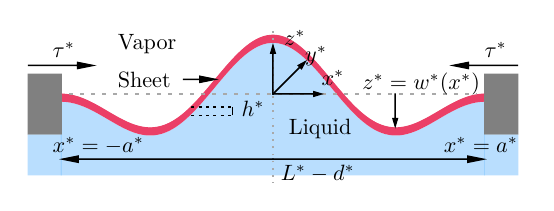
\begin{tikzpicture}

\definecolor{darkgray}{RGB}{169,169,169}
\definecolor{darkgray176}{RGB}{176,176,176}
\definecolor{gray}{RGB}{128,128,128}
\definecolor{indianred23563103}{RGB}{235,63,103}
\definecolor{lightskyblue138200253}{RGB}{138,200,253}

\begin{axis}[
axis equal image,
hide x axis,
hide y axis,
tick align=outside,
tick pos=left,
x grid style={darkgray176},
xlabel={0},
xmin=-0.03311, xmax=0.03311,
xtick style={color=black},
y grid style={darkgray176},
ymin=-0.010863663529839, ymax=0.00813693412661942,
ytick style={color=black}
]
\path [fill=lightskyblue138200253, fill opacity=0.6]
(axis cs:-0.0260467875630729,-0.00095)
--(axis cs:-0.0260467875630729,-0.00095)
--(axis cs:-0.0259887601975588,-0.000950265193764294)
--(axis cs:-0.0259307328320446,-0.000951060839657842)
--(axis cs:-0.0258727054665305,-0.000952386935837379)
--(axis cs:-0.0258146781010164,-0.000954243348798273)
--(axis cs:-0.0257566507355023,-0.000956629813394401)
--(axis cs:-0.0256986233699882,-0.000959545932885385)
--(axis cs:-0.0256405960044741,-0.0009629911790112)
--(axis cs:-0.02558256863896,-0.0009669648920941)
--(axis cs:-0.0255245412734459,-0.0009714662811679)
--(axis cs:-0.0254665139079318,-0.0009764944241347)
--(axis cs:-0.0254084865424177,-0.0009820482679484)
--(axis cs:-0.0253504591769036,-0.0009881266288259)
--(axis cs:-0.0252924318113895,-0.0009947281924857)
--(axis cs:-0.0252344044458754,-0.0010018515144127)
--(axis cs:-0.0251763770803613,-0.0010094950201512)
--(axis cs:-0.0251183497148472,-0.0010176570056243)
--(axis cs:-0.0250603223493331,-0.00102633563748)
--(axis cs:-0.025002294983819,-0.0010355289534653)
--(axis cs:-0.0249442676183049,-0.001045234862826)
--(axis cs:-0.0248862402527908,-0.0010554511467335)
--(axis cs:-0.0248282128872767,-0.0010661754587388)
--(axis cs:-0.0247701855217626,-0.0010774053252526)
--(axis cs:-0.0247121581562485,-0.0010891381460517)
--(axis cs:-0.0246541307907344,-0.0011013711948125)
--(axis cs:-0.0245961034252203,-0.00111410161967)
--(axis cs:-0.0245380760597062,-0.0011273264438032)
--(axis cs:-0.0244800486941921,-0.0011410425660469)
--(axis cs:-0.024422021328678,-0.001155246761529)
--(axis cs:-0.0243639939631638,-0.0011699356823334)
--(axis cs:-0.0243059665976497,-0.0011851058581895)
--(axis cs:-0.0242479392321356,-0.0012007536971861)
--(axis cs:-0.0241899118666215,-0.0012168754865111)
--(axis cs:-0.0241318845011074,-0.0012334673932171)
--(axis cs:-0.0240738571355933,-0.0012505254650108)
--(axis cs:-0.0240158297700792,-0.0012680456310682)
--(axis cs:-0.0239578024045651,-0.0012860237028747)
--(axis cs:-0.023899775039051,-0.0013044553750889)
--(axis cs:-0.0238417476735369,-0.0013233362264317)
--(axis cs:-0.0237837203080228,-0.0013426617205992)
--(axis cs:-0.0237256929425087,-0.0013624272071996)
--(axis cs:-0.0236676655769946,-0.0013826279227144)
--(axis cs:-0.0236096382114805,-0.0014032589914829)
--(axis cs:-0.0235516108459664,-0.00142431542671)
--(axis cs:-0.0234935834804523,-0.0014457921314979)
--(axis cs:-0.0234355561149382,-0.0014676838999004)
--(axis cs:-0.0233775287494241,-0.0014899854180001)
--(axis cs:-0.02331950138391,-0.0015126912650084)
--(axis cs:-0.0232614740183959,-0.001535795914388)
--(axis cs:-0.0232034466528818,-0.0015592937349971)
--(axis cs:-0.0231454192873677,-0.0015831789922564)
--(axis cs:-0.0230873919218536,-0.0016074458493369)
--(axis cs:-0.0230293645563395,-0.0016320883683701)
--(axis cs:-0.0229713371908254,-0.0016571005116786)
--(axis cs:-0.0229133098253113,-0.0016824761430286)
--(axis cs:-0.0228552824597972,-0.0017082090289024)
--(axis cs:-0.022797255094283,-0.0017342928397919)
--(axis cs:-0.0227392277287689,-0.0017607211515122)
--(axis cs:-0.0226812003632548,-0.0017874874465348)
--(axis cs:-0.0226231729977407,-0.0018145851153413)
--(axis cs:-0.0225651456322266,-0.0018420074577962)
--(axis cs:-0.0225071182667125,-0.0018697476845382)
--(axis cs:-0.0224490909011984,-0.0018977989183919)
--(axis cs:-0.0223910635356843,-0.0019261541957963)
--(axis cs:-0.0223330361701702,-0.0019548064682534)
--(axis cs:-0.0222750088046561,-0.0019837486037933)
--(axis cs:-0.022216981439142,-0.0020129733884583)
--(axis cs:-0.0221589540736279,-0.0020424735278035)
--(axis cs:-0.0221009267081138,-0.0020722416484151)
--(axis cs:-0.0220428993425997,-0.0021022702994453)
--(axis cs:-0.0219848719770856,-0.0021325519541642)
--(axis cs:-0.0219268446115715,-0.0021630790115269)
--(axis cs:-0.0218688172460574,-0.0021938437977579)
--(axis cs:-0.0218107898805433,-0.0022248385679495)
--(axis cs:-0.0217527625150292,-0.0022560555076774)
--(axis cs:-0.0216947351495151,-0.0022874867346291)
--(axis cs:-0.021636707784001,-0.002319124300249)
--(axis cs:-0.0215786804184869,-0.0023509601913962)
--(axis cs:-0.0215206530529728,-0.0023829863320169)
--(axis cs:-0.0214626256874587,-0.0024151945848308)
--(axis cs:-0.0214045983219446,-0.0024475767530302)
--(axis cs:-0.0213465709564305,-0.002480124581992)
--(axis cs:-0.0212885435909164,-0.0025128297610032)
--(axis cs:-0.0212305162254023,-0.0025456839249973)
--(axis cs:-0.0211724888598882,-0.002578678656304)
--(axis cs:-0.021114461494374,-0.0026118054864094)
--(axis cs:-0.0210564341288599,-0.0026450558977279)
--(axis cs:-0.0209984067633458,-0.0026784213253852)
--(axis cs:-0.0209403793978317,-0.002711893159011)
--(axis cs:-0.0208823520323176,-0.0027454627445428)
--(axis cs:-0.0208243246668035,-0.0027791213860387)
--(axis cs:-0.0207662973012894,-0.0028128603475)
--(axis cs:-0.0207082699357753,-0.0028466708547028)
--(axis cs:-0.0206502425702612,-0.0028805440970383)
--(axis cs:-0.0205922152047471,-0.0029144712293615)
--(axis cs:-0.020534187839233,-0.0029484433738474)
--(axis cs:-0.0204761604737189,-0.0029824516218552)
--(axis cs:-0.0204181331082048,-0.0030164870357999)
--(axis cs:-0.0203601057426907,-0.0030505406510301)
--(axis cs:-0.0203020783771766,-0.0030846034777124)
--(axis cs:-0.0202440510116625,-0.0031186665027225)
--(axis cs:-0.0201860236461484,-0.0031527206915414)
--(axis cs:-0.0201279962806343,-0.0031867569901566)
--(axis cs:-0.0200699689151202,-0.0032207663269691)
--(axis cs:-0.0200119415496061,-0.0032547396147045)
--(axis cs:-0.019953914184092,-0.0032886677523278)
--(axis cs:-0.0198958868185779,-0.0033225416269632)
--(axis cs:-0.0198378594530638,-0.0033563521158155)
--(axis cs:-0.0197798320875497,-0.0033900900880965)
--(axis cs:-0.0197218047220356,-0.0034237464069524)
--(axis cs:-0.0196637773565215,-0.0034573119313946)
--(axis cs:-0.0196057499910074,-0.0034907775182313)
--(axis cs:-0.0195477226254933,-0.0035241340240011)
--(axis cs:-0.0194896952599792,-0.0035573723069084)
--(axis cs:-0.019431667894465,-0.0035904832287575)
--(axis cs:-0.0193736405289509,-0.0036234576568893)
--(axis cs:-0.0193156131634368,-0.0036562864661163)
--(axis cs:-0.0192575857979227,-0.0036889605406574)
--(axis cs:-0.0191995584324086,-0.0037214707760725)
--(axis cs:-0.0191415310668945,-0.0037538080811952)
--(axis cs:-0.0190835037013804,-0.003785963380064)
--(axis cs:-0.0190254763358663,-0.0038179276138512)
--(axis cs:-0.0189674489703522,-0.0038496917427901)
--(axis cs:-0.0189094216048381,-0.0038812467480988)
--(axis cs:-0.018851394239324,-0.0039125836339006)
--(axis cs:-0.0187933668738099,-0.0039436934291412)
--(axis cs:-0.0187353395082958,-0.0039745671895024)
--(axis cs:-0.0186773121427817,-0.0040051959993101)
--(axis cs:-0.0186192847772676,-0.0040355709734386)
--(axis cs:-0.0185612574117535,-0.0040656832592097)
--(axis cs:-0.0185032300462394,-0.0040955240382859)
--(axis cs:-0.0184452026807253,-0.0041250845285578)
--(axis cs:-0.0183871753152112,-0.0041543559860256)
--(axis cs:-0.0183291479496971,-0.004183329706673)
--(axis cs:-0.018271120584183,-0.0042119970283357)
--(axis cs:-0.0182130932186689,-0.0042403493325605)
--(axis cs:-0.0181550658531548,-0.0042683780464584)
--(axis cs:-0.0180970384876407,-0.0042960746445482)
--(axis cs:-0.0180390111221266,-0.0043234306505924)
--(axis cs:-0.0179809837566125,-0.0043504376394242)
--(axis cs:-0.0179229563910984,-0.0043770872387641)
--(axis cs:-0.0178649290255843,-0.0044033711310288)
--(axis cs:-0.0178069016600702,-0.0044292810551283)
--(axis cs:-0.0177488742945561,-0.0044548088082534)
--(axis cs:-0.0176908469290419,-0.0044799462476529)
--(axis cs:-0.0176328195635278,-0.0045046852923988)
--(axis cs:-0.0175747921980137,-0.0045290179251406)
--(axis cs:-0.0175167648324996,-0.0045529361938479)
--(axis cs:-0.0174587374669855,-0.0045764322135405)
--(axis cs:-0.0174007101014714,-0.0045994981680062)
--(axis cs:-0.0173426827359573,-0.0046221263115058)
--(axis cs:-0.0172846553704432,-0.0046443089704646)
--(axis cs:-0.0172266280049291,-0.004666038545151)
--(axis cs:-0.017168600639415,-0.0046873075113404)
--(axis cs:-0.0171105732739009,-0.0047081084219658)
--(axis cs:-0.0170525459083868,-0.0047284339087529)
--(axis cs:-0.0169945185428727,-0.004748276683841)
--(axis cs:-0.0169364911773586,-0.0047676295413887)
--(axis cs:-0.0168784638118445,-0.0047864853591634)
--(axis cs:-0.0168204364463304,-0.004804837100116)
--(axis cs:-0.0167624090808163,-0.0048226778139384)
--(axis cs:-0.0167043817153022,-0.0048400006386051)
--(axis cs:-0.0166463543497881,-0.004856798801898)
--(axis cs:-0.016588326984274,-0.0048730656229136)
--(axis cs:-0.0165302996187599,-0.0048887945135536)
--(axis cs:-0.0164722722532458,-0.0049039789799969)
--(axis cs:-0.0164142448877317,-0.0049186126241543)
--(axis cs:-0.0163562175222176,-0.0049326891451044)
--(axis cs:-0.0162981901567035,-0.004946202340511)
--(axis cs:-0.0162401627911894,-0.0049591461080219)
--(axis cs:-0.0161821354256753,-0.0049715144466483)
--(axis cs:-0.0161241080601612,-0.0049833014581245)
--(axis cs:-0.016066080694647,-0.0049945013482481)
--(axis cs:-0.0160080533291329,-0.0050051084282006)
--(axis cs:-0.0159500259636188,-0.0050151171158466)
--(axis cs:-0.0158919985981047,-0.0050245219370138)
--(axis cs:-0.0158339712325906,-0.0050333175267513)
--(axis cs:-0.0157759438670765,-0.0050414986305666)
--(axis cs:-0.0157179165015624,-0.0050490601056428)
--(axis cs:-0.0156598891360483,-0.0050559969220319)
--(axis cs:-0.0156018617705342,-0.0050623041638287)
--(axis cs:-0.0155438344050201,-0.0050679770303207)
--(axis cs:-0.015485807039506,-0.0050730108371168)
--(axis cs:-0.0154277796739919,-0.0050774010172532)
--(axis cs:-0.0153697523084778,-0.0050811431222766)
--(axis cs:-0.0153117249429637,-0.005084232823304)
--(axis cs:-0.0152536975774496,-0.0050866659120601)
--(axis cs:-0.0151956702119355,-0.0050884383018905)
--(axis cs:-0.0151376428464214,-0.0050895460287518)
--(axis cs:-0.0150796154809073,-0.0050899852521776)
--(axis cs:-0.0150215881153932,-0.0050897522562207)
--(axis cs:-0.0149635607498791,-0.0050888434503707)
--(axis cs:-0.014905533384365,-0.005087255370448)
--(axis cs:-0.0148475060188509,-0.0050849846794718)
--(axis cs:-0.0147894786533368,-0.0050820281685051)
--(axis cs:-0.0147314512878227,-0.005078382757473)
--(axis cs:-0.0146734239223086,-0.0050740454959573)
--(axis cs:-0.0146153965567945,-0.005069013563965)
--(axis cs:-0.0145573691912804,-0.0050632842726713)
--(axis cs:-0.0144993418257662,-0.0050568550651379)
--(axis cs:-0.0144413144602522,-0.0050497235170041)
--(axis cs:-0.014383287094738,-0.0050418873371532)
--(axis cs:-0.0143252597292239,-0.0050333443683527)
--(axis cs:-0.0142672323637098,-0.0050240925878675)
--(axis cs:-0.0142092049981957,-0.0050141301080476)
--(axis cs:-0.0141511776326816,-0.0050034551768892)
--(axis cs:-0.0140931502671675,-0.0049920661785691)
--(axis cs:-0.0140351229016534,-0.0049799616339523)
--(axis cs:-0.0139770955361393,-0.0049671402010732)
--(axis cs:-0.0139190681706252,-0.0049536006755896)
--(axis cs:-0.0138610408051111,-0.0049393419912099)
--(axis cs:-0.013803013439597,-0.0049243632200929)
--(axis cs:-0.0137449860740829,-0.004908663573221)
--(axis cs:-0.0136869587085688,-0.0048922424007455)
--(axis cs:-0.0136289313430547,-0.0048750991923051)
--(axis cs:-0.0135709039775406,-0.0048572335773168)
--(axis cs:-0.0135128766120265,-0.0048386453252388)
--(axis cs:-0.0134548492465124,-0.0048193343458073)
--(axis cs:-0.0133968218809983,-0.0047993006892437)
--(axis cs:-0.0133387945154842,-0.0047785445464361)
--(axis cs:-0.0132807671499701,-0.004757066249092)
--(axis cs:-0.013222739784456,-0.0047348662698632)
--(axis cs:-0.0131647124189419,-0.0047119452224437)
--(axis cs:-0.0131066850534278,-0.0046883038616392)
--(axis cs:-0.0130486576879137,-0.0046639430834091)
--(axis cs:-0.0129906303223996,-0.0046388639248803)
--(axis cs:-0.0129326029568855,-0.0046130675643335)
--(axis cs:-0.0128745755913714,-0.0045865553211618)
--(axis cs:-0.0128165482258572,-0.0045593286558008)
--(axis cs:-0.0127585208603431,-0.0045313891696316)
--(axis cs:-0.012700493494829,-0.0045027386048555)
--(axis cs:-0.0126424661293149,-0.0044733788443407)
--(axis cs:-0.0125844387638008,-0.0044433119114421)
--(axis cs:-0.0125264113982867,-0.0044125399697922)
--(axis cs:-0.0124683840327726,-0.004381065323065)
--(axis cs:-0.0124103566672585,-0.0043488904147121)
--(axis cs:-0.0123523293017444,-0.0043160178276705)
--(axis cs:-0.0122943019362303,-0.0042824502840439)
--(axis cs:-0.0122362745707162,-0.0042481906447556)
--(axis cs:-0.0121782472052021,-0.0042132419091739)
--(axis cs:-0.012120219839688,-0.0041776072147107)
--(axis cs:-0.0120621924741739,-0.0041412898363918)
--(axis cs:-0.0120041651086598,-0.0041042931864011)
--(axis cs:-0.0119461377431457,-0.0040666208135963)
--(axis cs:-0.0118881103776316,-0.0040282764029982)
--(axis cs:-0.0118300830121175,-0.0039892637752531)
--(axis cs:-0.0117720556466034,-0.0039495868860678)
--(axis cs:-0.0117140282810893,-0.0039092498256181)
--(axis cs:-0.0116560009155752,-0.0038682568179303)
--(axis cs:-0.0115979735500611,-0.0038266122202361)
--(axis cs:-0.011539946184547,-0.0037843205223014)
--(axis cs:-0.0114819188190329,-0.0037413863457285)
--(axis cs:-0.0114238914535188,-0.0036978144432314)
--(axis cs:-0.0113658640880047,-0.0036536096978864)
--(axis cs:-0.0113078367224906,-0.003608777122355)
--(axis cs:-0.0112498093569765,-0.0035633218580827)
--(axis cs:-0.0111917819914624,-0.0035172491744708)
--(axis cs:-0.0111337546259482,-0.0034705644680232)
--(axis cs:-0.0110757272604341,-0.0034232732614678)
--(axis cs:-0.01101769989492,-0.0033753812028528)
--(axis cs:-0.0109596725294059,-0.0033268940646176)
--(axis cs:-0.0109016451638918,-0.0032778177426395)
--(axis cs:-0.0108436177983777,-0.0032281582552545)
--(axis cs:-0.0107855904328636,-0.0031779217422552)
--(axis cs:-0.0107275630673495,-0.0031271144638632)
--(axis cs:-0.0106695357018354,-0.0030757427996777)
--(axis cs:-0.0106115083363213,-0.0030238132476002)
--(axis cs:-0.0105534809708072,-0.002971332422736)
--(axis cs:-0.0104954536052931,-0.0029183070562708)
--(axis cs:-0.010437426239779,-0.0028647439943259)
--(axis cs:-0.0103793988742649,-0.0028106501967886)
--(axis cs:-0.0103213715087508,-0.0027560327361208)
--(axis cs:-0.0102633441432367,-0.0027008987961445)
--(axis cs:-0.0102053167777226,-0.0026452556708052)
--(axis cs:-0.0101472894122085,-0.0025891107629128)
--(axis cs:-0.0100892620466944,-0.0025324715828607)
--(axis cs:-0.0100312346811803,-0.0024753457473236)
--(axis cs:-0.0099732073156662,-0.002417740977933)
--(axis cs:-0.0099151799501521,-0.0023596650999325)
--(axis cs:-0.009857152584638,-0.0023011260408115)
--(axis cs:-0.0097991252191239,-0.0022421318289185)
--(axis cs:-0.0097410978536098,-0.0021826905920538)
--(axis cs:-0.0096830704880957,-0.0021228105560424)
--(axis cs:-0.0096250431225816,-0.002062500043287)
--(axis cs:-0.0095670157570675,-0.0020017674713008)
--(axis cs:-0.0095089883915534,-0.001940621351222)
--(axis cs:-0.0094509610260392,-0.0018790702863083)
--(axis cs:-0.0093929336605251,-0.0018171229704134)
--(axis cs:-0.009334906295011,-0.001754788186445)
--(axis cs:-0.0092768789294969,-0.0016920748048038)
--(axis cs:-0.0092188515639828,-0.0016289917818061)
--(axis cs:-0.0091608241984687,-0.0015655481580875)
--(axis cs:-0.0091027968329546,-0.0015017530569903)
--(axis cs:-0.0090447694674405,-0.0014376156829333)
--(axis cs:-0.0089867421019264,-0.0013731453197656)
--(axis cs:-0.0089287147364123,-0.0013083513291039)
--(axis cs:-0.0088706873708982,-0.0012432431486535)
--(axis cs:-0.0088126600053841,-0.0011778302905138)
--(axis cs:-0.00875463263987,-0.0011121223394691)
--(axis cs:-0.0086966052743559,-0.0010461289512635)
--(axis cs:-0.0086385779088418,-0.0009798598508618)
--(axis cs:-0.0085805505433277,-0.0009133248306954)
--(axis cs:-0.0085225231778136,-0.0008465337488949)
--(axis cs:-0.0084644958122995,-0.000779496527509)
--(axis cs:-0.0084064684467854,-0.0007122231507094)
--(axis cs:-0.0083484410812713,-0.0006447236629836)
--(axis cs:-0.0082904137157572,-0.0005770081673146)
--(axis cs:-0.0082323863502431,-0.0005090868233482)
--(axis cs:-0.008174358984729,-0.000440969845549)
--(axis cs:-0.0081163316192149,-0.0003726675013445)
--(axis cs:-0.0080583042537008,-0.0003041901092578)
--(axis cs:-0.0080002768881867,-0.0002355480370296)
--(axis cs:-0.0079422495226726,-0.0001667516997302)
--(axis cs:-0.0078842221571585,-9.78115578609e-05)
--(axis cs:-0.0078261947916443,-2.87381154455e-05)
--(axis cs:-0.0077681674261302,4.04580818869001e-05)
--(axis cs:-0.0077101400606161,0.0001097664488288)
--(axis cs:-0.007652112695102,0.000179176362329)
--(axis cs:-0.0075940853295879,0.0002486771635367)
--(axis cs:-0.0075360579640738,0.0003182581597521)
--(axis cs:-0.0074780305985597,0.0003879086263859)
--(axis cs:-0.0074200032330456,0.0004576178089245)
--(axis cs:-0.0073619758675315,0.0005273749249031)
--(axis cs:-0.0073039485020174,0.0005971691658846)
--(axis cs:-0.0072459211365033,0.0006669896994445)
--(axis cs:-0.0071878937709892,0.0007368256711616)
--(axis cs:-0.0071298664054751,0.0008066662066133)
--(axis cs:-0.007071839039961,0.0008765004133766)
--(axis cs:-0.0070138116744469,0.000946317383033)
--(axis cs:-0.0069557843089328,0.0010161061931771)
--(axis cs:-0.0068977569434187,0.0010858559094298)
--(axis cs:-0.0068397295779046,0.0011555555874539)
--(axis cs:-0.0067817022123905,0.0012251942749728)
--(axis cs:-0.0067236748468764,0.0012947610137919)
--(axis cs:-0.0066656474813623,0.0013642448418217)
--(axis cs:-0.0066076201158482,0.001433634795103)
--(axis cs:-0.0065495927503341,0.0015029199098332)
--(axis cs:-0.00649156538482,0.0015720892243932)
--(axis cs:-0.0064335380193059,0.0016411317813754)
--(axis cs:-0.0063755106537918,0.0017100366296114)
--(axis cs:-0.0063174832882777,0.0017787928261994)
--(axis cs:-0.0062594559227636,0.0018473894385313)
--(axis cs:-0.0062014285572495,0.0019158155463182)
--(axis cs:-0.0061434011917353,0.0019840602436151)
--(axis cs:-0.0060853738262212,0.0020521126408427)
--(axis cs:-0.0060273464607071,0.0021199618668086)
--(axis cs:-0.005969319095193,0.0021875970707238)
--(axis cs:-0.0059112917296789,0.002255007424218)
--(axis cs:-0.0058532643641648,0.0023221821233506)
--(axis cs:-0.0057952369986507,0.0023891103906177)
--(axis cs:-0.0057372096331366,0.0024557814769555)
--(axis cs:-0.0056791822676225,0.0025221846637386)
--(axis cs:-0.0056211549021084,0.0025883092647736)
--(axis cs:-0.0055631275365943,0.0026541446282875)
--(axis cs:-0.0055051001710802,0.0027196801389097)
--(axis cs:-0.0054470728055661,0.0027849052196483)
--(axis cs:-0.005389045440052,0.0028498093338603)
--(axis cs:-0.0053310180745379,0.0029143819872138)
--(axis cs:-0.0052729907090238,0.0029786127296439)
--(axis cs:-0.0052149633435097,0.0030424911573005)
--(axis cs:-0.0051569359779956,0.0031060069144879)
--(axis cs:-0.0050989086124815,0.0031691496955965)
--(axis cs:-0.0050408812469674,0.0032319092470251)
--(axis cs:-0.0049828538814533,0.0032942753690946)
--(axis cs:-0.0049248265159392,0.0033562379179513)
--(axis cs:-0.0048667991504251,0.0034177868074615)
--(axis cs:-0.004808771784911,0.0034789120110947)
--(axis cs:-0.0047507444193969,0.0035396035637965)
--(axis cs:-0.0046927170538828,0.003599851563851)
--(axis cs:-0.0046346896883687,0.0036596461747309)
--(axis cs:-0.0045766623228546,0.0037189776269367)
--(axis cs:-0.0045186349573404,0.0037778362198231)
--(axis cs:-0.0044606075918263,0.0038362123234136)
--(axis cs:-0.0044025802263122,0.0038940963802016)
--(axis cs:-0.0043445528607981,0.003951478906939)
--(axis cs:-0.004286525495284,0.0040083504964109)
--(axis cs:-0.0042284981297699,0.0040647018191964)
--(axis cs:-0.0041704707642558,0.0041205236254156)
--(axis cs:-0.0041124433987417,0.0041758067464615)
--(axis cs:-0.0040544160332276,0.0042305420967175)
--(axis cs:-0.0039963886677135,0.0042847206752595)
--(axis cs:-0.0039383613021994,0.0043383335675425)
--(axis cs:-0.0038803339366853,0.0043913719470711)
--(axis cs:-0.0038223065711712,0.0044438270770541)
--(axis cs:-0.0037642792056571,0.0044956903120428)
--(axis cs:-0.003706251840143,0.0045469530995516)
--(axis cs:-0.0036482244746289,0.0045976069816624)
--(axis cs:-0.0035901971091148,0.0046476435966109)
--(axis cs:-0.0035321697436007,0.0046970546803555)
--(axis cs:-0.0034741423780866,0.0047458320681279)
--(axis cs:-0.0034161150125725,0.0047939676959654)
--(axis cs:-0.0033580876470584,0.0048414536022244)
--(axis cs:-0.0033000602815443,0.0048882819290753)
--(axis cs:-0.0032420329160302,0.0049344449239776)
--(axis cs:-0.0031840055505161,0.0049799349411358)
--(axis cs:-0.003125978185002,0.0050247444429354)
--(axis cs:-0.0030679508194879,0.0050688660013585)
--(axis cs:-0.0030099234539738,0.0051122922993799)
--(axis cs:-0.0029518960884597,0.0051550161323409)
--(axis cs:-0.0028938687229456,0.0051970304093041)
--(axis cs:-0.0028358413574314,0.0052383281543854)
--(axis cs:-0.0027778139919173,0.0052789025080655)
--(axis cs:-0.0027197866264032,0.0053187467284794)
--(axis cs:-0.0026617592608891,0.0053578541926837)
--(axis cs:-0.002603731895375,0.0053962183979018)
--(axis cs:-0.0025457045298609,0.0054338329627473)
--(axis cs:-0.0024876771643468,0.0054706916284235)
--(axis cs:-0.0024296497988327,0.0055067882599011)
--(axis cs:-0.0023716224333186,0.0055421168470718)
--(axis cs:-0.0023135950678045,0.0055766715058794)
--(axis cs:-0.0022555677022904,0.0056104464794266)
--(axis cs:-0.0021975403367763,0.0056434361390583)
--(axis cs:-0.0021395129712622,0.0056756349854209)
--(axis cs:-0.0020814856057481,0.0057070376494972)
--(axis cs:-0.002023458240234,0.0057376388936169)
--(axis cs:-0.0019654308747199,0.0057674336124427)
--(axis cs:-0.0019074035092058,0.005796416833931)
--(axis cs:-0.0018493761436917,0.0058245837202684)
--(axis cs:-0.0017913487781776,0.0058519295687821)
--(axis cs:-0.0017333214126635,0.0058784498128259)
--(axis cs:-0.0016752940471494,0.0059041400226397)
--(axis cs:-0.0016172666816353,0.0059289959061837)
--(axis cs:-0.0015592393161212,0.0059530133099471)
--(axis cs:-0.0015012119506071,0.0059761882197301)
--(axis cs:-0.001443184585093,0.0059985167614001)
--(axis cs:-0.0013851572195789,0.0060199952016214)
--(axis cs:-0.0013271298540648,0.0060406199485585)
--(axis cs:-0.0012691024885507,0.006060387552553)
--(axis cs:-0.0012110751230365,0.0060792947067731)
--(axis cs:-0.0011530477575224,0.0060973382478368)
--(axis cs:-0.0010950203920083,0.0061145151564082)
--(axis cs:-0.0010369930264942,0.0061308225577661)
--(axis cs:-0.0009789656609801,0.0061462577223458)
--(axis cs:-0.000920938295466,0.0061608180662536)
--(axis cs:-0.0008629109299519,0.0061745011517535)
--(axis cs:-0.0008048835644378,0.0061873046877267)
--(axis cs:-0.0007468561989237,0.0061992265301038)
--(axis cs:-0.0006888288334096,0.0062102646822681)
--(axis cs:-0.0006308014678955,0.0062204172954327)
--(axis cs:-0.0005727741023814,0.0062296826689883)
--(axis cs:-0.0005147467368673,0.0062380592508244)
--(axis cs:-0.0004567193713532,0.0062455456376213)
--(axis cs:-0.0003986920058391,0.0062521405751149)
--(axis cs:-0.000340664640325,0.0062578429583332)
--(axis cs:-0.0002826372748109,0.0062626518318042)
--(axis cs:-0.0002246099092968,0.0062665663897367)
--(axis cs:-0.0001665825437827,0.0062695859761714)
--(axis cs:-0.0001085551782686,0.0062717100851051)
--(axis cs:-5.05278127545e-05,0.0062729383605859)
--(axis cs:7.49955275957484e-06,0.0062732705967804)
--(axis cs:6.55269182736e-05,0.0062727067380123)
--(axis cs:0.0001235542837877,0.0062712468787732)
--(axis cs:0.0001815816493018,0.0062688912637045)
--(axis cs:0.0002396090148159,0.0062656402875514)
--(axis cs:0.00029763638033,0.0062614944950884)
--(axis cs:0.0003556637458441,0.006256454581017)
--(axis cs:0.0004136911113583,0.006250521389834)
--(axis cs:0.0004717184768724,0.0062436959156731)
--(axis cs:0.0005297458423865,0.0062359793021168)
--(axis cs:0.0005877732079006,0.0062273728419815)
--(axis cs:0.0006458005734147,0.0062178779770732)
--(axis cs:0.0007038279389288,0.0062074962979162)
--(axis cs:0.0007618553044429,0.0061962295434529)
--(axis cs:0.000819882669957,0.0061840796007164)
--(axis cs:0.0008779100354711,0.0061710485044744)
--(axis cs:0.0009359374009852,0.0061571384368463)
--(axis cs:0.0009939647664993,0.0061423517268912)
--(axis cs:0.0010519921320134,0.0061266908501698)
--(axis cs:0.0011100194975275,0.0061101584282769)
--(axis cs:0.0011680468630416,0.0060927572283482)
--(axis cs:0.0012260742285557,0.0060744901625383)
--(axis cs:0.0012841015940698,0.0060553602874725)
--(axis cs:0.0013421289595839,0.0060353708036701)
--(axis cs:0.001400156325098,0.0060145250549421)
--(axis cs:0.0014581836906121,0.0059928265277606)
--(axis cs:0.0015162110561262,0.0059702788506027)
--(axis cs:0.0015742384216403,0.0059468857932659)
--(axis cs:0.0016322657871544,0.005922651266159)
--(axis cs:0.0016902931526685,0.0058975793195649)
--(axis cs:0.0017483205181826,0.0058716741428779)
--(axis cs:0.0018063478836967,0.0058449400638145)
--(axis cs:0.0018643752492108,0.0058173815475987)
--(axis cs:0.0019224026147249,0.0057890031961207)
--(axis cs:0.001980429980239,0.0057598097470708)
--(axis cs:0.0020384573457531,0.005729806073047)
--(axis cs:0.0020964847112673,0.0056989971806378)
--(axis cs:0.0021545120767814,0.0056673882094794)
--(axis cs:0.0022125394422955,0.0056349844312886)
--(axis cs:0.0022705668078096,0.0056017912488703)
--(axis cs:0.0023285941733237,0.0055678141951005)
--(axis cs:0.0023866215388378,0.0055330589318852)
--(axis cs:0.0024446489043519,0.0054975312490949)
--(axis cs:0.002502676269866,0.0054612370634753)
--(axis cs:0.0025607036353801,0.005424182417534)
--(axis cs:0.0026187310008942,0.0053863734784036)
--(axis cs:0.0026767583664083,0.0053478165366819)
--(axis cs:0.0027347857319224,0.0053085180052486)
--(axis cs:0.0027928130974365,0.0052684844180596)
--(axis cs:0.0028508404629506,0.0052277224289176)
--(axis cs:0.0029088678284647,0.0051862388102218)
--(axis cs:0.0029668951939788,0.0051440404516942)
--(axis cs:0.0030249225594929,0.0051011343590849)
--(axis cs:0.003082949925007,0.0050575276528549)
--(axis cs:0.0031409772905211,0.0050132275668382)
--(axis cs:0.0031990046560352,0.0049682414468826)
--(axis cs:0.0032570320215493,0.0049225767494693)
--(axis cs:0.0033150593870634,0.0048762410403122)
--(axis cs:0.0033730867525775,0.0048292419929372)
--(axis cs:0.0034311141180916,0.0047815873872405)
--(axis cs:0.0034891414836057,0.004733285108028)
--(axis cs:0.0035471688491198,0.0046843431435352)
--(axis cs:0.0036051962146339,0.0046347695839272)
--(axis cs:0.003663223580148,0.0045845726197802)
--(axis cs:0.0037212509456621,0.004533760540545)
--(axis cs:0.0037792783111762,0.004482341732991)
--(axis cs:0.0038373056766904,0.0044303246796332)
--(axis cs:0.0038953330422045,0.0043777179571411)
--(axis cs:0.0039533604077186,0.0043245302347299)
--(axis cs:0.0040113877732327,0.0042707702725355)
--(axis cs:0.0040694151387468,0.0042164469199718)
--(axis cs:0.0041274425042609,0.0041615691140721)
--(axis cs:0.004185469869775,0.0041061458778145)
--(axis cs:0.0042434972352891,0.0040501863184309)
--(axis cs:0.0043015246008032,0.0039936996257012)
--(axis cs:0.0043595519663173,0.0039366950702318)
--(axis cs:0.0044175793318314,0.0038791820017202)
--(axis cs:0.0044756066973455,0.0038211698472038)
--(axis cs:0.0045336340628596,0.003762668109296)
--(axis cs:0.0045916614283737,0.0037036863644075)
--(axis cs:0.0046496887938878,0.0036442342609547)
--(axis cs:0.0047077161594019,0.0035843215175549)
--(axis cs:0.004765743524916,0.0035239579212088)
--(axis cs:0.0048237708904301,0.0034631533254706)
--(axis cs:0.0048817982559442,0.0034019176486059)
--(axis cs:0.0049398256214583,0.0033402608717384)
--(axis cs:0.0049978529869724,0.0032781930369852)
--(axis cs:0.0050558803524865,0.0032157242455805)
--(axis cs:0.0051139077180006,0.0031528646559898)
--(axis cs:0.0051719350835147,0.003089624482013)
--(axis cs:0.0052299624490288,0.0030260139908785)
--(axis cs:0.0052879898145429,0.0029620435013268)
--(axis cs:0.005346017180057,0.0028977233816861)
--(axis cs:0.0054040445455711,0.0028330640479385)
--(axis cs:0.0054620719110853,0.0027680759617783)
--(axis cs:0.0055200992765994,0.0027027696286617)
--(axis cs:0.0055781266421135,0.0026371555958498)
--(axis cs:0.0056361540076276,0.0025712444504435)
--(axis cs:0.0056941813731417,0.0025050468174126)
--(axis cs:0.0057522087386558,0.0024385733576175)
--(axis cs:0.0058102361041699,0.0023718347658253)
--(axis cs:0.005868263469684,0.0023048417687207)
--(axis cs:0.0059262908351981,0.0022376051229103)
--(axis cs:0.0059843182007122,0.0021701356129237)
--(axis cs:0.0060423455662263,0.0021024440492087)
--(axis cs:0.0061003729317404,0.0020345412661233)
--(axis cs:0.0061584002972545,0.0019664381199237)
--(axis cs:0.0062164276627686,0.0018981454867484)
--(axis cs:0.0062744550282827,0.0018296742606007)
--(axis cs:0.0063324823937968,0.0017610353513271)
--(axis cs:0.0063905097593109,0.001692239682595)
--(axis cs:0.006448537124825,0.0016232981898673)
--(axis cs:0.0065065644903391,0.001554221818377)
--(axis cs:0.0065645918558532,0.0014850215210994)
--(axis cs:0.0066226192213673,0.0014157082567252)
--(axis cs:0.0066806465868814,0.001346292987632)
--(axis cs:0.0067386739523955,0.0012767866778573)
--(axis cs:0.0067967013179096,0.0012072002910712)
--(axis cs:0.0068547286834237,0.0011375447885503)
--(axis cs:0.0069127560489378,0.0010678311271533)
--(axis cs:0.0069707834144519,0.0009980702572983)
--(axis cs:0.007028810779966,0.0009282731209418)
--(axis cs:0.0070868381454802,0.0008584506495611)
--(axis cs:0.0071448655109943,0.0007886137621388)
--(axis cs:0.0072028928765084,0.0007187733631513)
--(axis cs:0.0072609202420225,0.0006489403405607)
--(axis cs:0.0073189476075366,0.0005791255638111)
--(axis cs:0.0073769749730507,0.000509339881829)
--(axis cs:0.0074350023385648,0.0004395941210292)
--(axis cs:0.0074930297040789,0.0003698990833254)
--(axis cs:0.007551057069593,0.0003002655441467)
--(axis cs:0.0076090844351071,0.0002307042504607)
--(axis cs:0.0076671118006212,0.0001612259188018)
--(axis cs:0.0077251391661353,9.1841233308e-05)
--(axis cs:0.0077831665316494,2.2560843763e-05)
--(axis cs:0.0078411938971635,-4.6604636352e-05)
--(axis cs:0.0078992212626776,-0.0001156446318008)
--(axis cs:0.0079572486281917,-0.0001845486075241)
--(axis cs:0.0080152759937058,-0.0002533060705646)
--(axis cs:0.0080733033592199,-0.0003219065719818)
--(axis cs:0.008131330724734,-0.0003903397087577)
--(axis cs:0.0081893580902481,-0.0004585951256928)
--(axis cs:0.0082473854557622,-0.0005266625172919)
--(axis cs:0.0083054128212763,-0.0005945316296392)
--(axis cs:0.0083634401867904,-0.0006621922622624)
--(axis cs:0.0084214675523045,-0.0007296342699856)
--(axis cs:0.0084794949178186,-0.000796847564771)
--(axis cs:0.0085375222833327,-0.0008638221175477)
--(axis cs:0.0085955496488468,-0.0009305479600291)
--(axis cs:0.0086535770143609,-0.0009970151865167)
--(axis cs:0.0087116043798751,-0.001063213955692)
--(axis cs:0.0087696317453892,-0.0011291344923936)
--(axis cs:0.0088276591109033,-0.0011947670893817)
--(axis cs:0.0088856864764174,-0.001260102109088)
--(axis cs:0.0089437138419315,-0.0013251299853514)
--(axis cs:0.0090017412074456,-0.0013898412251388)
--(axis cs:0.0090597685729597,-0.0014542264102508)
--(axis cs:0.0091177959384738,-0.0015182761990121)
--(axis cs:0.0091758233039879,-0.0015819813279464)
--(axis cs:0.009233850669502,-0.0016453326134344)
--(axis cs:0.0092918780350161,-0.0017083209533569)
--(axis cs:0.0093499054005302,-0.0017709373287194)
--(axis cs:0.0094079327660443,-0.0018331728052611)
--(axis cs:0.0094659601315584,-0.0018950185350463)
--(axis cs:0.0095239874970725,-0.0019564657580374)
--(axis cs:0.0095820148625866,-0.0020175058036514)
--(axis cs:0.0096400422281007,-0.0020781300922963)
--(axis cs:0.0096980695936148,-0.0021383301368913)
--(axis cs:0.0097560969591289,-0.0021980975443657)
--(axis cs:0.009814124324643,-0.002257424017141)
--(axis cs:0.0098721516901571,-0.0023163013545921)
--(axis cs:0.0099301790556712,-0.0023747214544891)
--(axis cs:0.0099882064211853,-0.0024326763144199)
--(axis cs:0.0100462337866994,-0.002490158033192)
--(axis cs:0.0101042611522135,-0.0025471588122137)
--(axis cs:0.0101622885177276,-0.0026036709568549)
--(axis cs:0.0102203158832417,-0.0026596868777869)
--(axis cs:0.0102783432487558,-0.0027151990923009)
--(axis cs:0.01033637061427,-0.0027702002256047)
--(axis cs:0.0103943979797841,-0.0028246830120981)
--(axis cs:0.0104524253452982,-0.0028786402966263)
--(axis cs:0.0105104527108123,-0.0029320650357105)
--(axis cs:0.0105684800763264,-0.0029849502987567)
--(axis cs:0.0106265074418405,-0.0030372892692415)
--(axis cs:0.0106845348073546,-0.0030890752458751)
--(axis cs:0.0107425621728687,-0.0031403016437409)
--(axis cs:0.0108005895383828,-0.0031909619954122)
--(axis cs:0.0108586169038969,-0.0032410499520447)
--(axis cs:0.010916644269411,-0.003290559284446)
--(axis cs:0.0109746716349251,-0.0033394838841205)
--(axis cs:0.0110326990004392,-0.0033878177642905)
--(axis cs:0.0110907263659533,-0.0034355550608927)
--(axis cs:0.0111487537314674,-0.0034826900335504)
--(axis cs:0.0112067810969815,-0.0035292170665205)
--(axis cs:0.0112648084624956,-0.0035751306696162)
--(axis cs:0.0113228358280097,-0.0036204254791044)
--(axis cs:0.0113808631935238,-0.0036650962585775)
--(axis cs:0.0114388905590379,-0.0037091378998003)
--(axis cs:0.011496917924552,-0.0037525454235308)
--(axis cs:0.0115549452900661,-0.0037953139803162)
--(axis cs:0.0116129726555802,-0.0038374388512615)
--(axis cs:0.0116710000210943,-0.0038789154487739)
--(axis cs:0.0117290273866084,-0.0039197393172793)
--(axis cs:0.0117870547521225,-0.0039599061339142)
--(axis cs:0.0118450821176366,-0.0039994117091896)
--(axis cs:0.0119031094831507,-0.0040382519876296)
--(axis cs:0.0119611368486648,-0.0040764230483826)
--(axis cs:0.012019164214179,-0.0041139211058063)
--(axis cs:0.0120771915796931,-0.0041507425100251)
--(axis cs:0.0121352189452072,-0.0041868837474614)
--(axis cs:0.0121932463107213,-0.0042223414413392)
--(axis cs:0.0122512736762354,-0.004257112352161)
--(axis cs:0.0123093010417495,-0.0042911933781567)
--(axis cs:0.0123673284072636,-0.0043245815557064)
--(axis cs:0.0124253557727777,-0.0043572740597346)
--(axis cs:0.0124833831382918,-0.0043892682040776)
--(axis cs:0.0125414105038059,-0.0044205614418237)
--(axis cs:0.01259943786932,-0.0044511513656245)
--(axis cs:0.0126574652348341,-0.0044810357079803)
--(axis cs:0.0127154926003482,-0.0045102123414964)
--(axis cs:0.0127735199658623,-0.0045386792791127)
--(axis cs:0.0128315473313764,-0.0045664346743046)
--(axis cs:0.0128895746968905,-0.0045934768212569)
--(axis cs:0.0129476020624046,-0.0046198041550099)
--(axis cs:0.0130056294279187,-0.0046454152515768)
--(axis cs:0.0130636567934328,-0.0046703088280343)
--(axis cs:0.0131216841589469,-0.0046944837425845)
--(axis cs:0.013179711524461,-0.0047179389945898)
--(axis cs:0.0132377388899751,-0.0047406737245792)
--(axis cs:0.0132957662554892,-0.0047626872142272)
--(axis cs:0.0133537936210033,-0.0047839788863046)
--(axis cs:0.0134118209865174,-0.0048045483046017)
--(axis cs:0.0134698483520315,-0.0048243951738238)
--(axis cs:0.0135278757175456,-0.0048435193394584)
--(axis cs:0.0135859030830597,-0.0048619207876156)
--(axis cs:0.0136439304485738,-0.0048795996448399)
--(axis cs:0.013701957814088,-0.004896556177895)
--(axis cs:0.0137599851796021,-0.0049127907935207)
--(axis cs:0.0138180125451162,-0.0049283040381624)
--(axis cs:0.0138760399106303,-0.0049430965976733)
--(axis cs:0.0139340672761444,-0.0049571692969887)
--(axis cs:0.0139920946416585,-0.0049705230997738)
--(axis cs:0.0140501220071726,-0.0049831591080435)
--(axis cs:0.0141081493726867,-0.0049950785617552)
--(axis cs:0.0141661767382008,-0.0050062828383751)
--(axis cs:0.0142242041037149,-0.0050167734524172)
--(axis cs:0.014282231469229,-0.0050265520549547)
--(axis cs:0.0143402588347431,-0.005035620433106)
--(axis cs:0.0143982862002572,-0.0050439805094931)
--(axis cs:0.0144563135657713,-0.0050516343416738)
--(axis cs:0.0145143409312854,-0.0050585841215475)
--(axis cs:0.0145723682967995,-0.0050648321747344)
--(axis cs:0.0146303956623136,-0.0050703809599292)
--(axis cs:0.0146884230278277,-0.0050752330682281)
--(axis cs:0.0147464503933418,-0.0050793912224305)
--(axis cs:0.0148044777588559,-0.0050828582763143)
--(axis cs:0.01486250512437,-0.0050856372138866)
--(axis cs:0.0149205324898841,-0.0050877311486079)
--(axis cs:0.0149785598553982,-0.0050891433225921)
--(axis cs:0.0150365872209123,-0.0050898771057806)
--(axis cs:0.0150946145864264,-0.0050899359950916)
--(axis cs:0.0151526419519405,-0.0050893236135455)
--(axis cs:0.0152106693174546,-0.0050880437093646)
--(axis cs:0.0152686966829687,-0.005086100155049)
--(axis cs:0.0153267240484828,-0.0050834969464287)
--(axis cs:0.015384751413997,-0.0050802382016908)
--(axis cs:0.0154427787795111,-0.0050763281603838)
--(axis cs:0.0155008061450252,-0.0050717711823979)
--(axis cs:0.0155588335105393,-0.005066571746922)
--(axis cs:0.0156168608760534,-0.0050607344513776)
--(axis cs:0.0156748882415675,-0.0050542640103297)
--(axis cs:0.0157329156070816,-0.0050471652543753)
--(axis cs:0.0157909429725957,-0.005039443129009)
--(axis cs:0.0158489703381098,-0.0050311026934667)
--(axis cs:0.0159069977036239,-0.005022149119547)
--(axis cs:0.015965025069138,-0.0050125876904114)
--(axis cs:0.0160230524346521,-0.0050024237993623)
--(axis cs:0.0160810798001662,-0.0049916629485999)
--(axis cs:0.0161391071656803,-0.004980310747959)
--(axis cs:0.0161971345311944,-0.0049683729136234)
--(axis cs:0.0162551618967085,-0.0049558552668215)
--(axis cs:0.0163131892622226,-0.0049427637325003)
--(axis cs:0.0163712166277367,-0.0049291043379807)
--(axis cs:0.0164292439932508,-0.0049148832115919)
--(axis cs:0.0164872713587649,-0.0049001065812876)
--(axis cs:0.016545298724279,-0.004884780773242)
--(axis cs:0.0166033260897931,-0.0048689122104278)
--(axis cs:0.0166613534553072,-0.0048525074111753)
--(axis cs:0.0167193808208213,-0.0048355729877132)
--(axis cs:0.0167774081863354,-0.0048181156446917)
--(axis cs:0.0168354355518495,-0.004800142177688)
--(axis cs:0.0168934629173636,-0.0047816594716938)
--(axis cs:0.0169514902828777,-0.0047626744995868)
--(axis cs:0.0170095176483918,-0.0047431943205846)
--(axis cs:0.0170675450139059,-0.0047232260786827)
--(axis cs:0.0171255723794201,-0.0047027770010761)
--(axis cs:0.0171835997449342,-0.0046818543965657)
--(axis cs:0.0172416271104483,-0.004660465653948)
--(axis cs:0.0172996544759624,-0.0046386182403917)
--(axis cs:0.0173576818414765,-0.0046163196997972)
--(axis cs:0.0174157092069906,-0.0045935776511434)
--(axis cs:0.0174737365725047,-0.0045703997868196)
--(axis cs:0.0175317639380188,-0.0045467938709439)
--(axis cs:0.0175897913035329,-0.0045227677376678)
--(axis cs:0.017647818669047,-0.0044983292894679)
--(axis cs:0.0177058460345611,-0.0044734864954251)
--(axis cs:0.0177638734000752,-0.0044482473894911)
--(axis cs:0.0178219007655893,-0.0044226200687427)
--(axis cs:0.0178799281311034,-0.0043966126916248)
--(axis cs:0.0179379554966175,-0.004370233476182)
--(axis cs:0.0179959828621316,-0.0043434906982784)
--(axis cs:0.0180540102276457,-0.0043163926898083)
--(axis cs:0.0181120375931598,-0.0042889478368951)
--(axis cs:0.0181700649586739,-0.0042611645780812)
--(axis cs:0.018228092324188,-0.0042330514025082)
--(axis cs:0.0182861196897021,-0.0042046168480877)
--(axis cs:0.0183441470552162,-0.0041758694996633)
--(axis cs:0.0184021744207303,-0.0041468179871646)
--(axis cs:0.0184602017862444,-0.0041174709837527)
--(axis cs:0.0185182291517585,-0.004087837203958)
--(axis cs:0.0185762565172726,-0.0040579254018111)
--(axis cs:0.0186342838827868,-0.0040277443689661)
--(axis cs:0.0186923112483009,-0.0039973029328184)
--(axis cs:0.018750338613815,-0.0039666099546148)
--(axis cs:0.0188083659793291,-0.0039356743275595)
--(axis cs:0.0188663933448432,-0.0039045049749132)
--(axis cs:0.0189244207103573,-0.0038731108480883)
--(axis cs:0.0189824480758714,-0.0038415009247386)
--(axis cs:0.0190404754413855,-0.0038096842068452)
--(axis cs:0.0190985028068996,-0.0037776697187986)
--(axis cs:0.0191565301724137,-0.003745466505477)
--(axis cs:0.0192145575379278,-0.0037130836303214)
--(axis cs:0.0192725849034419,-0.0036805301734087)
--(axis cs:0.019330612268956,-0.0036478152295214)
--(axis cs:0.0193886396344701,-0.0036149479062165)
--(axis cs:0.0194466669999842,-0.0035819373218916)
--(axis cs:0.0195046943654983,-0.0035487926038511)
--(axis cs:0.0195627217310124,-0.0035155228863709)
--(axis cs:0.0196207490965265,-0.0034821373087624)
--(axis cs:0.0196787764620406,-0.0034486450134374)
--(axis cs:0.0197368038275547,-0.003415055143973)
--(axis cs:0.0197948311930688,-0.0033813768431766)
--(axis cs:0.0198528585585829,-0.0033476192511534)
--(axis cs:0.019910885924097,-0.003313791503374)
--(axis cs:0.0199689132896111,-0.0032799027287454)
--(axis cs:0.0200269406551252,-0.0032459620476829)
--(axis cs:0.0200849680206393,-0.0032119785701862)
--(axis cs:0.0201429953861534,-0.0031779613939168)
--(axis cs:0.0202010227516675,-0.0031439196022808)
--(axis cs:0.0202590501171816,-0.0031098622625145)
--(axis cs:0.0203170774826958,-0.0030757984237739)
--(axis cs:0.0203751048482099,-0.0030417371152301)
--(axis cs:0.020433132213724,-0.0030076873441686)
--(axis cs:0.0204911595792381,-0.0029736580940943)
--(axis cs:0.0205491869447522,-0.0029396583228431)
--(axis cs:0.0206072143102663,-0.002905696960698)
--(axis cs:0.0206652416757804,-0.0028717829085135)
--(axis cs:0.0207232690412945,-0.0028379250358456)
--(axis cs:0.0207812964068086,-0.00280413217909)
--(axis cs:0.0208393237723227,-0.0027704131396275)
--(axis cs:0.0208973511378368,-0.0027367766819773)
--(axis cs:0.0209553785033509,-0.0027032315319593)
--(axis cs:0.021013405868865,-0.0026697863748646)
--(axis cs:0.0210714332343791,-0.0026364498536353)
--(axis cs:0.0211294605998932,-0.0026032305670542)
--(axis cs:0.0211874879654073,-0.0025701370679438)
--(axis cs:0.0212455153309214,-0.0025371778613758)
--(axis cs:0.0213035426964355,-0.0025043614028912)
--(axis cs:0.0213615700619496,-0.0024716960967314)
--(axis cs:0.0214195974274637,-0.0024391902940805)
--(axis cs:0.0214776247929778,-0.0024068522913194)
--(axis cs:0.0215356521584919,-0.0023746903282914)
--(axis cs:0.021593679524006,-0.0023427125865812)
--(axis cs:0.0216517068895201,-0.0023109271878053)
--(axis cs:0.0217097342550342,-0.0022793421919166)
--(axis cs:0.0217677616205483,-0.0022479655955214)
--(axis cs:0.0218257889860624,-0.0022168053302111)
--(axis cs:0.0218838163515765,-0.002185869260907)
--(axis cs:0.0219418437170906,-0.0021551651842204)
--(axis cs:0.0219998710826047,-0.0021247008268264)
--(axis cs:0.0220578984481189,-0.0020944838438535)
--(axis cs:0.022115925813633,-0.0020645218172886)
--(axis cs:0.0221739531791471,-0.002034822254397)
--(axis cs:0.0222319805446612,-0.002005392586159)
--(axis cs:0.0222900079101753,-0.0019762401657228)
--(axis cs:0.0223480352756894,-0.0019473722668735)
--(axis cs:0.0224060626412035,-0.0019187960825194)
--(axis cs:0.0224640900067176,-0.0018905187231959)
--(axis cs:0.0225221173722317,-0.0018625472155858)
--(axis cs:0.0225801447377458,-0.001834888501059)
--(axis cs:0.0226381721032599,-0.0018075494342286)
--(axis cs:0.022696199468774,-0.001780536781527)
--(axis cs:0.0227542268342881,-0.0017538572197993)
--(axis cs:0.0228122541998022,-0.0017275173349169)
--(axis cs:0.0228702815653163,-0.0017015236204093)
--(axis cs:0.0229283089308304,-0.0016758824761162)
--(axis cs:0.0229863362963445,-0.0016506002068587)
--(axis cs:0.0230443636618586,-0.0016256830211315)
--(axis cs:0.0231023910273727,-0.0016011370298143)
--(axis cs:0.0231604183928868,-0.0015769682449047)
--(axis cs:0.0232184457584009,-0.0015531825782712)
--(axis cs:0.023276473123915,-0.0015297858404283)
--(axis cs:0.0233345004894291,-0.0015067837393312)
--(axis cs:0.0233925278549432,-0.0014841818791942)
--(axis cs:0.0234505552204573,-0.0014619857593291)
--(axis cs:0.0235085825859714,-0.0014402007730068)
--(axis cs:0.0235666099514855,-0.0014188322063404)
--(axis cs:0.0236246373169996,-0.0013978852371913)
--(axis cs:0.0236826646825138,-0.0013773649340976)
--(axis cs:0.0237406920480279,-0.001357276255226)
--(axis cs:0.023798719413542,-0.0013376240473459)
--(axis cs:0.0238567467790561,-0.001318413044828)
--(axis cs:0.0239147741445702,-0.0012996478686653)
--(axis cs:0.0239728015100843,-0.0012813330255186)
--(axis cs:0.0240308288755984,-0.0012634729067854)
--(axis cs:0.0240888562411125,-0.0012460717876937)
--(axis cs:0.0241468836066266,-0.0012291338264189)
--(axis cs:0.0242049109721407,-0.0012126630632262)
--(axis cs:0.0242629383376548,-0.0011966634196371)
--(axis cs:0.0243209657031689,-0.0011811386976208)
--(axis cs:0.024378993068683,-0.0011660925788107)
--(axis cs:0.0244370204341971,-0.0011515286237458)
--(axis cs:0.0244950477997112,-0.0011374502711378)
--(axis cs:0.0245530751652253,-0.0011238608371628)
--(axis cs:0.0246111025307394,-0.0011107635147792)
--(axis cs:0.0246691298962535,-0.0010981613730714)
--(axis cs:0.0247271572617676,-0.0010860573566189)
--(axis cs:0.0247851846272817,-0.0010744542848915)
--(axis cs:0.0248432119927958,-0.0010633548516704)
--(axis cs:0.0249012393583099,-0.0010527616244961)
--(axis cs:0.024959266723824,-0.0010426770441417)
--(axis cs:0.0250172940893381,-0.0010331034241136)
--(axis cs:0.0250753214548522,-0.0010240429501774)
--(axis cs:0.0251333488203663,-0.0010154976799119)
--(axis cs:0.0251913761858804,-0.0010074695422888)
--(axis cs:0.0252494035513945,-0.000999960337279)
--(axis cs:0.0253074309169086,-0.0009929717354868)
--(axis cs:0.0253654582824227,-0.00098650527781)
--(axis cs:0.0254234856479369,-0.0009805623751273)
--(axis cs:0.025481513013451,-0.000975144308013)
--(axis cs:0.0255395403789651,-0.0009702522264785)
--(axis cs:0.0255975677444792,-0.0009658871497411)
--(axis cs:0.0256555951099933,-0.0009620499660201)
--(axis cs:0.0257136224755074,-0.000958741432359484)
--(axis cs:0.0257716498410215,-0.000955962174479068)
--(axis cs:0.0258296772065356,-0.000953712686651917)
--(axis cs:0.0258877045720497,-0.00095199333160954)
--(axis cs:0.0259457319375638,-0.000950804340474359)
--(axis cs:0.0260037593030779,-0.000950145812719545)
--(axis cs:0.0260037593030779,-0.000950145812719545)
--(axis cs:0.0260037593030779,-0.01)
--(axis cs:0.0259457319375638,-0.01)
--(axis cs:0.0258877045720497,-0.01)
--(axis cs:0.0258296772065356,-0.01)
--(axis cs:0.0257716498410215,-0.01)
--(axis cs:0.0257136224755074,-0.01)
--(axis cs:0.0256555951099933,-0.01)
--(axis cs:0.0255975677444792,-0.01)
--(axis cs:0.0255395403789651,-0.01)
--(axis cs:0.025481513013451,-0.01)
--(axis cs:0.0254234856479369,-0.01)
--(axis cs:0.0253654582824227,-0.01)
--(axis cs:0.0253074309169086,-0.01)
--(axis cs:0.0252494035513945,-0.01)
--(axis cs:0.0251913761858804,-0.01)
--(axis cs:0.0251333488203663,-0.01)
--(axis cs:0.0250753214548522,-0.01)
--(axis cs:0.0250172940893381,-0.01)
--(axis cs:0.024959266723824,-0.01)
--(axis cs:0.0249012393583099,-0.01)
--(axis cs:0.0248432119927958,-0.01)
--(axis cs:0.0247851846272817,-0.01)
--(axis cs:0.0247271572617676,-0.01)
--(axis cs:0.0246691298962535,-0.01)
--(axis cs:0.0246111025307394,-0.01)
--(axis cs:0.0245530751652253,-0.01)
--(axis cs:0.0244950477997112,-0.01)
--(axis cs:0.0244370204341971,-0.01)
--(axis cs:0.024378993068683,-0.01)
--(axis cs:0.0243209657031689,-0.01)
--(axis cs:0.0242629383376548,-0.01)
--(axis cs:0.0242049109721407,-0.01)
--(axis cs:0.0241468836066266,-0.01)
--(axis cs:0.0240888562411125,-0.01)
--(axis cs:0.0240308288755984,-0.01)
--(axis cs:0.0239728015100843,-0.01)
--(axis cs:0.0239147741445702,-0.01)
--(axis cs:0.0238567467790561,-0.01)
--(axis cs:0.023798719413542,-0.01)
--(axis cs:0.0237406920480279,-0.01)
--(axis cs:0.0236826646825138,-0.01)
--(axis cs:0.0236246373169996,-0.01)
--(axis cs:0.0235666099514855,-0.01)
--(axis cs:0.0235085825859714,-0.01)
--(axis cs:0.0234505552204573,-0.01)
--(axis cs:0.0233925278549432,-0.01)
--(axis cs:0.0233345004894291,-0.01)
--(axis cs:0.023276473123915,-0.01)
--(axis cs:0.0232184457584009,-0.01)
--(axis cs:0.0231604183928868,-0.01)
--(axis cs:0.0231023910273727,-0.01)
--(axis cs:0.0230443636618586,-0.01)
--(axis cs:0.0229863362963445,-0.01)
--(axis cs:0.0229283089308304,-0.01)
--(axis cs:0.0228702815653163,-0.01)
--(axis cs:0.0228122541998022,-0.01)
--(axis cs:0.0227542268342881,-0.01)
--(axis cs:0.022696199468774,-0.01)
--(axis cs:0.0226381721032599,-0.01)
--(axis cs:0.0225801447377458,-0.01)
--(axis cs:0.0225221173722317,-0.01)
--(axis cs:0.0224640900067176,-0.01)
--(axis cs:0.0224060626412035,-0.01)
--(axis cs:0.0223480352756894,-0.01)
--(axis cs:0.0222900079101753,-0.01)
--(axis cs:0.0222319805446612,-0.01)
--(axis cs:0.0221739531791471,-0.01)
--(axis cs:0.022115925813633,-0.01)
--(axis cs:0.0220578984481189,-0.01)
--(axis cs:0.0219998710826047,-0.01)
--(axis cs:0.0219418437170906,-0.01)
--(axis cs:0.0218838163515765,-0.01)
--(axis cs:0.0218257889860624,-0.01)
--(axis cs:0.0217677616205483,-0.01)
--(axis cs:0.0217097342550342,-0.01)
--(axis cs:0.0216517068895201,-0.01)
--(axis cs:0.021593679524006,-0.01)
--(axis cs:0.0215356521584919,-0.01)
--(axis cs:0.0214776247929778,-0.01)
--(axis cs:0.0214195974274637,-0.01)
--(axis cs:0.0213615700619496,-0.01)
--(axis cs:0.0213035426964355,-0.01)
--(axis cs:0.0212455153309214,-0.01)
--(axis cs:0.0211874879654073,-0.01)
--(axis cs:0.0211294605998932,-0.01)
--(axis cs:0.0210714332343791,-0.01)
--(axis cs:0.021013405868865,-0.01)
--(axis cs:0.0209553785033509,-0.01)
--(axis cs:0.0208973511378368,-0.01)
--(axis cs:0.0208393237723227,-0.01)
--(axis cs:0.0207812964068086,-0.01)
--(axis cs:0.0207232690412945,-0.01)
--(axis cs:0.0206652416757804,-0.01)
--(axis cs:0.0206072143102663,-0.01)
--(axis cs:0.0205491869447522,-0.01)
--(axis cs:0.0204911595792381,-0.01)
--(axis cs:0.020433132213724,-0.01)
--(axis cs:0.0203751048482099,-0.01)
--(axis cs:0.0203170774826958,-0.01)
--(axis cs:0.0202590501171816,-0.01)
--(axis cs:0.0202010227516675,-0.01)
--(axis cs:0.0201429953861534,-0.01)
--(axis cs:0.0200849680206393,-0.01)
--(axis cs:0.0200269406551252,-0.01)
--(axis cs:0.0199689132896111,-0.01)
--(axis cs:0.019910885924097,-0.01)
--(axis cs:0.0198528585585829,-0.01)
--(axis cs:0.0197948311930688,-0.01)
--(axis cs:0.0197368038275547,-0.01)
--(axis cs:0.0196787764620406,-0.01)
--(axis cs:0.0196207490965265,-0.01)
--(axis cs:0.0195627217310124,-0.01)
--(axis cs:0.0195046943654983,-0.01)
--(axis cs:0.0194466669999842,-0.01)
--(axis cs:0.0193886396344701,-0.01)
--(axis cs:0.019330612268956,-0.01)
--(axis cs:0.0192725849034419,-0.01)
--(axis cs:0.0192145575379278,-0.01)
--(axis cs:0.0191565301724137,-0.01)
--(axis cs:0.0190985028068996,-0.01)
--(axis cs:0.0190404754413855,-0.01)
--(axis cs:0.0189824480758714,-0.01)
--(axis cs:0.0189244207103573,-0.01)
--(axis cs:0.0188663933448432,-0.01)
--(axis cs:0.0188083659793291,-0.01)
--(axis cs:0.018750338613815,-0.01)
--(axis cs:0.0186923112483009,-0.01)
--(axis cs:0.0186342838827868,-0.01)
--(axis cs:0.0185762565172726,-0.01)
--(axis cs:0.0185182291517585,-0.01)
--(axis cs:0.0184602017862444,-0.01)
--(axis cs:0.0184021744207303,-0.01)
--(axis cs:0.0183441470552162,-0.01)
--(axis cs:0.0182861196897021,-0.01)
--(axis cs:0.018228092324188,-0.01)
--(axis cs:0.0181700649586739,-0.01)
--(axis cs:0.0181120375931598,-0.01)
--(axis cs:0.0180540102276457,-0.01)
--(axis cs:0.0179959828621316,-0.01)
--(axis cs:0.0179379554966175,-0.01)
--(axis cs:0.0178799281311034,-0.01)
--(axis cs:0.0178219007655893,-0.01)
--(axis cs:0.0177638734000752,-0.01)
--(axis cs:0.0177058460345611,-0.01)
--(axis cs:0.017647818669047,-0.01)
--(axis cs:0.0175897913035329,-0.01)
--(axis cs:0.0175317639380188,-0.01)
--(axis cs:0.0174737365725047,-0.01)
--(axis cs:0.0174157092069906,-0.01)
--(axis cs:0.0173576818414765,-0.01)
--(axis cs:0.0172996544759624,-0.01)
--(axis cs:0.0172416271104483,-0.01)
--(axis cs:0.0171835997449342,-0.01)
--(axis cs:0.0171255723794201,-0.01)
--(axis cs:0.0170675450139059,-0.01)
--(axis cs:0.0170095176483918,-0.01)
--(axis cs:0.0169514902828777,-0.01)
--(axis cs:0.0168934629173636,-0.01)
--(axis cs:0.0168354355518495,-0.01)
--(axis cs:0.0167774081863354,-0.01)
--(axis cs:0.0167193808208213,-0.01)
--(axis cs:0.0166613534553072,-0.01)
--(axis cs:0.0166033260897931,-0.01)
--(axis cs:0.016545298724279,-0.01)
--(axis cs:0.0164872713587649,-0.01)
--(axis cs:0.0164292439932508,-0.01)
--(axis cs:0.0163712166277367,-0.01)
--(axis cs:0.0163131892622226,-0.01)
--(axis cs:0.0162551618967085,-0.01)
--(axis cs:0.0161971345311944,-0.01)
--(axis cs:0.0161391071656803,-0.01)
--(axis cs:0.0160810798001662,-0.01)
--(axis cs:0.0160230524346521,-0.01)
--(axis cs:0.015965025069138,-0.01)
--(axis cs:0.0159069977036239,-0.01)
--(axis cs:0.0158489703381098,-0.01)
--(axis cs:0.0157909429725957,-0.01)
--(axis cs:0.0157329156070816,-0.01)
--(axis cs:0.0156748882415675,-0.01)
--(axis cs:0.0156168608760534,-0.01)
--(axis cs:0.0155588335105393,-0.01)
--(axis cs:0.0155008061450252,-0.01)
--(axis cs:0.0154427787795111,-0.01)
--(axis cs:0.015384751413997,-0.01)
--(axis cs:0.0153267240484828,-0.01)
--(axis cs:0.0152686966829687,-0.01)
--(axis cs:0.0152106693174546,-0.01)
--(axis cs:0.0151526419519405,-0.01)
--(axis cs:0.0150946145864264,-0.01)
--(axis cs:0.0150365872209123,-0.01)
--(axis cs:0.0149785598553982,-0.01)
--(axis cs:0.0149205324898841,-0.01)
--(axis cs:0.01486250512437,-0.01)
--(axis cs:0.0148044777588559,-0.01)
--(axis cs:0.0147464503933418,-0.01)
--(axis cs:0.0146884230278277,-0.01)
--(axis cs:0.0146303956623136,-0.01)
--(axis cs:0.0145723682967995,-0.01)
--(axis cs:0.0145143409312854,-0.01)
--(axis cs:0.0144563135657713,-0.01)
--(axis cs:0.0143982862002572,-0.01)
--(axis cs:0.0143402588347431,-0.01)
--(axis cs:0.014282231469229,-0.01)
--(axis cs:0.0142242041037149,-0.01)
--(axis cs:0.0141661767382008,-0.01)
--(axis cs:0.0141081493726867,-0.01)
--(axis cs:0.0140501220071726,-0.01)
--(axis cs:0.0139920946416585,-0.01)
--(axis cs:0.0139340672761444,-0.01)
--(axis cs:0.0138760399106303,-0.01)
--(axis cs:0.0138180125451162,-0.01)
--(axis cs:0.0137599851796021,-0.01)
--(axis cs:0.013701957814088,-0.01)
--(axis cs:0.0136439304485738,-0.01)
--(axis cs:0.0135859030830597,-0.01)
--(axis cs:0.0135278757175456,-0.01)
--(axis cs:0.0134698483520315,-0.01)
--(axis cs:0.0134118209865174,-0.01)
--(axis cs:0.0133537936210033,-0.01)
--(axis cs:0.0132957662554892,-0.01)
--(axis cs:0.0132377388899751,-0.01)
--(axis cs:0.013179711524461,-0.01)
--(axis cs:0.0131216841589469,-0.01)
--(axis cs:0.0130636567934328,-0.01)
--(axis cs:0.0130056294279187,-0.01)
--(axis cs:0.0129476020624046,-0.01)
--(axis cs:0.0128895746968905,-0.01)
--(axis cs:0.0128315473313764,-0.01)
--(axis cs:0.0127735199658623,-0.01)
--(axis cs:0.0127154926003482,-0.01)
--(axis cs:0.0126574652348341,-0.01)
--(axis cs:0.01259943786932,-0.01)
--(axis cs:0.0125414105038059,-0.01)
--(axis cs:0.0124833831382918,-0.01)
--(axis cs:0.0124253557727777,-0.01)
--(axis cs:0.0123673284072636,-0.01)
--(axis cs:0.0123093010417495,-0.01)
--(axis cs:0.0122512736762354,-0.01)
--(axis cs:0.0121932463107213,-0.01)
--(axis cs:0.0121352189452072,-0.01)
--(axis cs:0.0120771915796931,-0.01)
--(axis cs:0.012019164214179,-0.01)
--(axis cs:0.0119611368486648,-0.01)
--(axis cs:0.0119031094831507,-0.01)
--(axis cs:0.0118450821176366,-0.01)
--(axis cs:0.0117870547521225,-0.01)
--(axis cs:0.0117290273866084,-0.01)
--(axis cs:0.0116710000210943,-0.01)
--(axis cs:0.0116129726555802,-0.01)
--(axis cs:0.0115549452900661,-0.01)
--(axis cs:0.011496917924552,-0.01)
--(axis cs:0.0114388905590379,-0.01)
--(axis cs:0.0113808631935238,-0.01)
--(axis cs:0.0113228358280097,-0.01)
--(axis cs:0.0112648084624956,-0.01)
--(axis cs:0.0112067810969815,-0.01)
--(axis cs:0.0111487537314674,-0.01)
--(axis cs:0.0110907263659533,-0.01)
--(axis cs:0.0110326990004392,-0.01)
--(axis cs:0.0109746716349251,-0.01)
--(axis cs:0.010916644269411,-0.01)
--(axis cs:0.0108586169038969,-0.01)
--(axis cs:0.0108005895383828,-0.01)
--(axis cs:0.0107425621728687,-0.01)
--(axis cs:0.0106845348073546,-0.01)
--(axis cs:0.0106265074418405,-0.01)
--(axis cs:0.0105684800763264,-0.01)
--(axis cs:0.0105104527108123,-0.01)
--(axis cs:0.0104524253452982,-0.01)
--(axis cs:0.0103943979797841,-0.01)
--(axis cs:0.01033637061427,-0.01)
--(axis cs:0.0102783432487558,-0.01)
--(axis cs:0.0102203158832417,-0.01)
--(axis cs:0.0101622885177276,-0.01)
--(axis cs:0.0101042611522135,-0.01)
--(axis cs:0.0100462337866994,-0.01)
--(axis cs:0.0099882064211853,-0.01)
--(axis cs:0.0099301790556712,-0.01)
--(axis cs:0.0098721516901571,-0.01)
--(axis cs:0.009814124324643,-0.01)
--(axis cs:0.0097560969591289,-0.01)
--(axis cs:0.0096980695936148,-0.01)
--(axis cs:0.0096400422281007,-0.01)
--(axis cs:0.0095820148625866,-0.01)
--(axis cs:0.0095239874970725,-0.01)
--(axis cs:0.0094659601315584,-0.01)
--(axis cs:0.0094079327660443,-0.01)
--(axis cs:0.0093499054005302,-0.01)
--(axis cs:0.0092918780350161,-0.01)
--(axis cs:0.009233850669502,-0.01)
--(axis cs:0.0091758233039879,-0.01)
--(axis cs:0.0091177959384738,-0.01)
--(axis cs:0.0090597685729597,-0.01)
--(axis cs:0.0090017412074456,-0.01)
--(axis cs:0.0089437138419315,-0.01)
--(axis cs:0.0088856864764174,-0.01)
--(axis cs:0.0088276591109033,-0.01)
--(axis cs:0.0087696317453892,-0.01)
--(axis cs:0.0087116043798751,-0.01)
--(axis cs:0.0086535770143609,-0.01)
--(axis cs:0.0085955496488468,-0.01)
--(axis cs:0.0085375222833327,-0.01)
--(axis cs:0.0084794949178186,-0.01)
--(axis cs:0.0084214675523045,-0.01)
--(axis cs:0.0083634401867904,-0.01)
--(axis cs:0.0083054128212763,-0.01)
--(axis cs:0.0082473854557622,-0.01)
--(axis cs:0.0081893580902481,-0.01)
--(axis cs:0.008131330724734,-0.01)
--(axis cs:0.0080733033592199,-0.01)
--(axis cs:0.0080152759937058,-0.01)
--(axis cs:0.0079572486281917,-0.01)
--(axis cs:0.0078992212626776,-0.01)
--(axis cs:0.0078411938971635,-0.01)
--(axis cs:0.0077831665316494,-0.01)
--(axis cs:0.0077251391661353,-0.01)
--(axis cs:0.0076671118006212,-0.01)
--(axis cs:0.0076090844351071,-0.01)
--(axis cs:0.007551057069593,-0.01)
--(axis cs:0.0074930297040789,-0.01)
--(axis cs:0.0074350023385648,-0.01)
--(axis cs:0.0073769749730507,-0.01)
--(axis cs:0.0073189476075366,-0.01)
--(axis cs:0.0072609202420225,-0.01)
--(axis cs:0.0072028928765084,-0.01)
--(axis cs:0.0071448655109943,-0.01)
--(axis cs:0.0070868381454802,-0.01)
--(axis cs:0.007028810779966,-0.01)
--(axis cs:0.0069707834144519,-0.01)
--(axis cs:0.0069127560489378,-0.01)
--(axis cs:0.0068547286834237,-0.01)
--(axis cs:0.0067967013179096,-0.01)
--(axis cs:0.0067386739523955,-0.01)
--(axis cs:0.0066806465868814,-0.01)
--(axis cs:0.0066226192213673,-0.01)
--(axis cs:0.0065645918558532,-0.01)
--(axis cs:0.0065065644903391,-0.01)
--(axis cs:0.006448537124825,-0.01)
--(axis cs:0.0063905097593109,-0.01)
--(axis cs:0.0063324823937968,-0.01)
--(axis cs:0.0062744550282827,-0.01)
--(axis cs:0.0062164276627686,-0.01)
--(axis cs:0.0061584002972545,-0.01)
--(axis cs:0.0061003729317404,-0.01)
--(axis cs:0.0060423455662263,-0.01)
--(axis cs:0.0059843182007122,-0.01)
--(axis cs:0.0059262908351981,-0.01)
--(axis cs:0.005868263469684,-0.01)
--(axis cs:0.0058102361041699,-0.01)
--(axis cs:0.0057522087386558,-0.01)
--(axis cs:0.0056941813731417,-0.01)
--(axis cs:0.0056361540076276,-0.01)
--(axis cs:0.0055781266421135,-0.01)
--(axis cs:0.0055200992765994,-0.01)
--(axis cs:0.0054620719110853,-0.01)
--(axis cs:0.0054040445455711,-0.01)
--(axis cs:0.005346017180057,-0.01)
--(axis cs:0.0052879898145429,-0.01)
--(axis cs:0.0052299624490288,-0.01)
--(axis cs:0.0051719350835147,-0.01)
--(axis cs:0.0051139077180006,-0.01)
--(axis cs:0.0050558803524865,-0.01)
--(axis cs:0.0049978529869724,-0.01)
--(axis cs:0.0049398256214583,-0.01)
--(axis cs:0.0048817982559442,-0.01)
--(axis cs:0.0048237708904301,-0.01)
--(axis cs:0.004765743524916,-0.01)
--(axis cs:0.0047077161594019,-0.01)
--(axis cs:0.0046496887938878,-0.01)
--(axis cs:0.0045916614283737,-0.01)
--(axis cs:0.0045336340628596,-0.01)
--(axis cs:0.0044756066973455,-0.01)
--(axis cs:0.0044175793318314,-0.01)
--(axis cs:0.0043595519663173,-0.01)
--(axis cs:0.0043015246008032,-0.01)
--(axis cs:0.0042434972352891,-0.01)
--(axis cs:0.004185469869775,-0.01)
--(axis cs:0.0041274425042609,-0.01)
--(axis cs:0.0040694151387468,-0.01)
--(axis cs:0.0040113877732327,-0.01)
--(axis cs:0.0039533604077186,-0.01)
--(axis cs:0.0038953330422045,-0.01)
--(axis cs:0.0038373056766904,-0.01)
--(axis cs:0.0037792783111762,-0.01)
--(axis cs:0.0037212509456621,-0.01)
--(axis cs:0.003663223580148,-0.01)
--(axis cs:0.0036051962146339,-0.01)
--(axis cs:0.0035471688491198,-0.01)
--(axis cs:0.0034891414836057,-0.01)
--(axis cs:0.0034311141180916,-0.01)
--(axis cs:0.0033730867525775,-0.01)
--(axis cs:0.0033150593870634,-0.01)
--(axis cs:0.0032570320215493,-0.01)
--(axis cs:0.0031990046560352,-0.01)
--(axis cs:0.0031409772905211,-0.01)
--(axis cs:0.003082949925007,-0.01)
--(axis cs:0.0030249225594929,-0.01)
--(axis cs:0.0029668951939788,-0.01)
--(axis cs:0.0029088678284647,-0.01)
--(axis cs:0.0028508404629506,-0.01)
--(axis cs:0.0027928130974365,-0.01)
--(axis cs:0.0027347857319224,-0.01)
--(axis cs:0.0026767583664083,-0.01)
--(axis cs:0.0026187310008942,-0.01)
--(axis cs:0.0025607036353801,-0.01)
--(axis cs:0.002502676269866,-0.01)
--(axis cs:0.0024446489043519,-0.01)
--(axis cs:0.0023866215388378,-0.01)
--(axis cs:0.0023285941733237,-0.01)
--(axis cs:0.0022705668078096,-0.01)
--(axis cs:0.0022125394422955,-0.01)
--(axis cs:0.0021545120767814,-0.01)
--(axis cs:0.0020964847112673,-0.01)
--(axis cs:0.0020384573457531,-0.01)
--(axis cs:0.001980429980239,-0.01)
--(axis cs:0.0019224026147249,-0.01)
--(axis cs:0.0018643752492108,-0.01)
--(axis cs:0.0018063478836967,-0.01)
--(axis cs:0.0017483205181826,-0.01)
--(axis cs:0.0016902931526685,-0.01)
--(axis cs:0.0016322657871544,-0.01)
--(axis cs:0.0015742384216403,-0.01)
--(axis cs:0.0015162110561262,-0.01)
--(axis cs:0.0014581836906121,-0.01)
--(axis cs:0.001400156325098,-0.01)
--(axis cs:0.0013421289595839,-0.01)
--(axis cs:0.0012841015940698,-0.01)
--(axis cs:0.0012260742285557,-0.01)
--(axis cs:0.0011680468630416,-0.01)
--(axis cs:0.0011100194975275,-0.01)
--(axis cs:0.0010519921320134,-0.01)
--(axis cs:0.0009939647664993,-0.01)
--(axis cs:0.0009359374009852,-0.01)
--(axis cs:0.0008779100354711,-0.01)
--(axis cs:0.000819882669957,-0.01)
--(axis cs:0.0007618553044429,-0.01)
--(axis cs:0.0007038279389288,-0.01)
--(axis cs:0.0006458005734147,-0.01)
--(axis cs:0.0005877732079006,-0.01)
--(axis cs:0.0005297458423865,-0.01)
--(axis cs:0.0004717184768724,-0.01)
--(axis cs:0.0004136911113583,-0.01)
--(axis cs:0.0003556637458441,-0.01)
--(axis cs:0.00029763638033,-0.01)
--(axis cs:0.0002396090148159,-0.01)
--(axis cs:0.0001815816493018,-0.01)
--(axis cs:0.0001235542837877,-0.01)
--(axis cs:6.55269182736e-05,-0.01)
--(axis cs:7.49955275957484e-06,-0.01)
--(axis cs:-5.05278127545e-05,-0.01)
--(axis cs:-0.0001085551782686,-0.01)
--(axis cs:-0.0001665825437827,-0.01)
--(axis cs:-0.0002246099092968,-0.01)
--(axis cs:-0.0002826372748109,-0.01)
--(axis cs:-0.000340664640325,-0.01)
--(axis cs:-0.0003986920058391,-0.01)
--(axis cs:-0.0004567193713532,-0.01)
--(axis cs:-0.0005147467368673,-0.01)
--(axis cs:-0.0005727741023814,-0.01)
--(axis cs:-0.0006308014678955,-0.01)
--(axis cs:-0.0006888288334096,-0.01)
--(axis cs:-0.0007468561989237,-0.01)
--(axis cs:-0.0008048835644378,-0.01)
--(axis cs:-0.0008629109299519,-0.01)
--(axis cs:-0.000920938295466,-0.01)
--(axis cs:-0.0009789656609801,-0.01)
--(axis cs:-0.0010369930264942,-0.01)
--(axis cs:-0.0010950203920083,-0.01)
--(axis cs:-0.0011530477575224,-0.01)
--(axis cs:-0.0012110751230365,-0.01)
--(axis cs:-0.0012691024885507,-0.01)
--(axis cs:-0.0013271298540648,-0.01)
--(axis cs:-0.0013851572195789,-0.01)
--(axis cs:-0.001443184585093,-0.01)
--(axis cs:-0.0015012119506071,-0.01)
--(axis cs:-0.0015592393161212,-0.01)
--(axis cs:-0.0016172666816353,-0.01)
--(axis cs:-0.0016752940471494,-0.01)
--(axis cs:-0.0017333214126635,-0.01)
--(axis cs:-0.0017913487781776,-0.01)
--(axis cs:-0.0018493761436917,-0.01)
--(axis cs:-0.0019074035092058,-0.01)
--(axis cs:-0.0019654308747199,-0.01)
--(axis cs:-0.002023458240234,-0.01)
--(axis cs:-0.0020814856057481,-0.01)
--(axis cs:-0.0021395129712622,-0.01)
--(axis cs:-0.0021975403367763,-0.01)
--(axis cs:-0.0022555677022904,-0.01)
--(axis cs:-0.0023135950678045,-0.01)
--(axis cs:-0.0023716224333186,-0.01)
--(axis cs:-0.0024296497988327,-0.01)
--(axis cs:-0.0024876771643468,-0.01)
--(axis cs:-0.0025457045298609,-0.01)
--(axis cs:-0.002603731895375,-0.01)
--(axis cs:-0.0026617592608891,-0.01)
--(axis cs:-0.0027197866264032,-0.01)
--(axis cs:-0.0027778139919173,-0.01)
--(axis cs:-0.0028358413574314,-0.01)
--(axis cs:-0.0028938687229456,-0.01)
--(axis cs:-0.0029518960884597,-0.01)
--(axis cs:-0.0030099234539738,-0.01)
--(axis cs:-0.0030679508194879,-0.01)
--(axis cs:-0.003125978185002,-0.01)
--(axis cs:-0.0031840055505161,-0.01)
--(axis cs:-0.0032420329160302,-0.01)
--(axis cs:-0.0033000602815443,-0.01)
--(axis cs:-0.0033580876470584,-0.01)
--(axis cs:-0.0034161150125725,-0.01)
--(axis cs:-0.0034741423780866,-0.01)
--(axis cs:-0.0035321697436007,-0.01)
--(axis cs:-0.0035901971091148,-0.01)
--(axis cs:-0.0036482244746289,-0.01)
--(axis cs:-0.003706251840143,-0.01)
--(axis cs:-0.0037642792056571,-0.01)
--(axis cs:-0.0038223065711712,-0.01)
--(axis cs:-0.0038803339366853,-0.01)
--(axis cs:-0.0039383613021994,-0.01)
--(axis cs:-0.0039963886677135,-0.01)
--(axis cs:-0.0040544160332276,-0.01)
--(axis cs:-0.0041124433987417,-0.01)
--(axis cs:-0.0041704707642558,-0.01)
--(axis cs:-0.0042284981297699,-0.01)
--(axis cs:-0.004286525495284,-0.01)
--(axis cs:-0.0043445528607981,-0.01)
--(axis cs:-0.0044025802263122,-0.01)
--(axis cs:-0.0044606075918263,-0.01)
--(axis cs:-0.0045186349573404,-0.01)
--(axis cs:-0.0045766623228546,-0.01)
--(axis cs:-0.0046346896883687,-0.01)
--(axis cs:-0.0046927170538828,-0.01)
--(axis cs:-0.0047507444193969,-0.01)
--(axis cs:-0.004808771784911,-0.01)
--(axis cs:-0.0048667991504251,-0.01)
--(axis cs:-0.0049248265159392,-0.01)
--(axis cs:-0.0049828538814533,-0.01)
--(axis cs:-0.0050408812469674,-0.01)
--(axis cs:-0.0050989086124815,-0.01)
--(axis cs:-0.0051569359779956,-0.01)
--(axis cs:-0.0052149633435097,-0.01)
--(axis cs:-0.0052729907090238,-0.01)
--(axis cs:-0.0053310180745379,-0.01)
--(axis cs:-0.005389045440052,-0.01)
--(axis cs:-0.0054470728055661,-0.01)
--(axis cs:-0.0055051001710802,-0.01)
--(axis cs:-0.0055631275365943,-0.01)
--(axis cs:-0.0056211549021084,-0.01)
--(axis cs:-0.0056791822676225,-0.01)
--(axis cs:-0.0057372096331366,-0.01)
--(axis cs:-0.0057952369986507,-0.01)
--(axis cs:-0.0058532643641648,-0.01)
--(axis cs:-0.0059112917296789,-0.01)
--(axis cs:-0.005969319095193,-0.01)
--(axis cs:-0.0060273464607071,-0.01)
--(axis cs:-0.0060853738262212,-0.01)
--(axis cs:-0.0061434011917353,-0.01)
--(axis cs:-0.0062014285572495,-0.01)
--(axis cs:-0.0062594559227636,-0.01)
--(axis cs:-0.0063174832882777,-0.01)
--(axis cs:-0.0063755106537918,-0.01)
--(axis cs:-0.0064335380193059,-0.01)
--(axis cs:-0.00649156538482,-0.01)
--(axis cs:-0.0065495927503341,-0.01)
--(axis cs:-0.0066076201158482,-0.01)
--(axis cs:-0.0066656474813623,-0.01)
--(axis cs:-0.0067236748468764,-0.01)
--(axis cs:-0.0067817022123905,-0.01)
--(axis cs:-0.0068397295779046,-0.01)
--(axis cs:-0.0068977569434187,-0.01)
--(axis cs:-0.0069557843089328,-0.01)
--(axis cs:-0.0070138116744469,-0.01)
--(axis cs:-0.007071839039961,-0.01)
--(axis cs:-0.0071298664054751,-0.01)
--(axis cs:-0.0071878937709892,-0.01)
--(axis cs:-0.0072459211365033,-0.01)
--(axis cs:-0.0073039485020174,-0.01)
--(axis cs:-0.0073619758675315,-0.01)
--(axis cs:-0.0074200032330456,-0.01)
--(axis cs:-0.0074780305985597,-0.01)
--(axis cs:-0.0075360579640738,-0.01)
--(axis cs:-0.0075940853295879,-0.01)
--(axis cs:-0.007652112695102,-0.01)
--(axis cs:-0.0077101400606161,-0.01)
--(axis cs:-0.0077681674261302,-0.01)
--(axis cs:-0.0078261947916443,-0.01)
--(axis cs:-0.0078842221571585,-0.01)
--(axis cs:-0.0079422495226726,-0.01)
--(axis cs:-0.0080002768881867,-0.01)
--(axis cs:-0.0080583042537008,-0.01)
--(axis cs:-0.0081163316192149,-0.01)
--(axis cs:-0.008174358984729,-0.01)
--(axis cs:-0.0082323863502431,-0.01)
--(axis cs:-0.0082904137157572,-0.01)
--(axis cs:-0.0083484410812713,-0.01)
--(axis cs:-0.0084064684467854,-0.01)
--(axis cs:-0.0084644958122995,-0.01)
--(axis cs:-0.0085225231778136,-0.01)
--(axis cs:-0.0085805505433277,-0.01)
--(axis cs:-0.0086385779088418,-0.01)
--(axis cs:-0.0086966052743559,-0.01)
--(axis cs:-0.00875463263987,-0.01)
--(axis cs:-0.0088126600053841,-0.01)
--(axis cs:-0.0088706873708982,-0.01)
--(axis cs:-0.0089287147364123,-0.01)
--(axis cs:-0.0089867421019264,-0.01)
--(axis cs:-0.0090447694674405,-0.01)
--(axis cs:-0.0091027968329546,-0.01)
--(axis cs:-0.0091608241984687,-0.01)
--(axis cs:-0.0092188515639828,-0.01)
--(axis cs:-0.0092768789294969,-0.01)
--(axis cs:-0.009334906295011,-0.01)
--(axis cs:-0.0093929336605251,-0.01)
--(axis cs:-0.0094509610260392,-0.01)
--(axis cs:-0.0095089883915534,-0.01)
--(axis cs:-0.0095670157570675,-0.01)
--(axis cs:-0.0096250431225816,-0.01)
--(axis cs:-0.0096830704880957,-0.01)
--(axis cs:-0.0097410978536098,-0.01)
--(axis cs:-0.0097991252191239,-0.01)
--(axis cs:-0.009857152584638,-0.01)
--(axis cs:-0.0099151799501521,-0.01)
--(axis cs:-0.0099732073156662,-0.01)
--(axis cs:-0.0100312346811803,-0.01)
--(axis cs:-0.0100892620466944,-0.01)
--(axis cs:-0.0101472894122085,-0.01)
--(axis cs:-0.0102053167777226,-0.01)
--(axis cs:-0.0102633441432367,-0.01)
--(axis cs:-0.0103213715087508,-0.01)
--(axis cs:-0.0103793988742649,-0.01)
--(axis cs:-0.010437426239779,-0.01)
--(axis cs:-0.0104954536052931,-0.01)
--(axis cs:-0.0105534809708072,-0.01)
--(axis cs:-0.0106115083363213,-0.01)
--(axis cs:-0.0106695357018354,-0.01)
--(axis cs:-0.0107275630673495,-0.01)
--(axis cs:-0.0107855904328636,-0.01)
--(axis cs:-0.0108436177983777,-0.01)
--(axis cs:-0.0109016451638918,-0.01)
--(axis cs:-0.0109596725294059,-0.01)
--(axis cs:-0.01101769989492,-0.01)
--(axis cs:-0.0110757272604341,-0.01)
--(axis cs:-0.0111337546259482,-0.01)
--(axis cs:-0.0111917819914624,-0.01)
--(axis cs:-0.0112498093569765,-0.01)
--(axis cs:-0.0113078367224906,-0.01)
--(axis cs:-0.0113658640880047,-0.01)
--(axis cs:-0.0114238914535188,-0.01)
--(axis cs:-0.0114819188190329,-0.01)
--(axis cs:-0.011539946184547,-0.01)
--(axis cs:-0.0115979735500611,-0.01)
--(axis cs:-0.0116560009155752,-0.01)
--(axis cs:-0.0117140282810893,-0.01)
--(axis cs:-0.0117720556466034,-0.01)
--(axis cs:-0.0118300830121175,-0.01)
--(axis cs:-0.0118881103776316,-0.01)
--(axis cs:-0.0119461377431457,-0.01)
--(axis cs:-0.0120041651086598,-0.01)
--(axis cs:-0.0120621924741739,-0.01)
--(axis cs:-0.012120219839688,-0.01)
--(axis cs:-0.0121782472052021,-0.01)
--(axis cs:-0.0122362745707162,-0.01)
--(axis cs:-0.0122943019362303,-0.01)
--(axis cs:-0.0123523293017444,-0.01)
--(axis cs:-0.0124103566672585,-0.01)
--(axis cs:-0.0124683840327726,-0.01)
--(axis cs:-0.0125264113982867,-0.01)
--(axis cs:-0.0125844387638008,-0.01)
--(axis cs:-0.0126424661293149,-0.01)
--(axis cs:-0.012700493494829,-0.01)
--(axis cs:-0.0127585208603431,-0.01)
--(axis cs:-0.0128165482258572,-0.01)
--(axis cs:-0.0128745755913714,-0.01)
--(axis cs:-0.0129326029568855,-0.01)
--(axis cs:-0.0129906303223996,-0.01)
--(axis cs:-0.0130486576879137,-0.01)
--(axis cs:-0.0131066850534278,-0.01)
--(axis cs:-0.0131647124189419,-0.01)
--(axis cs:-0.013222739784456,-0.01)
--(axis cs:-0.0132807671499701,-0.01)
--(axis cs:-0.0133387945154842,-0.01)
--(axis cs:-0.0133968218809983,-0.01)
--(axis cs:-0.0134548492465124,-0.01)
--(axis cs:-0.0135128766120265,-0.01)
--(axis cs:-0.0135709039775406,-0.01)
--(axis cs:-0.0136289313430547,-0.01)
--(axis cs:-0.0136869587085688,-0.01)
--(axis cs:-0.0137449860740829,-0.01)
--(axis cs:-0.013803013439597,-0.01)
--(axis cs:-0.0138610408051111,-0.01)
--(axis cs:-0.0139190681706252,-0.01)
--(axis cs:-0.0139770955361393,-0.01)
--(axis cs:-0.0140351229016534,-0.01)
--(axis cs:-0.0140931502671675,-0.01)
--(axis cs:-0.0141511776326816,-0.01)
--(axis cs:-0.0142092049981957,-0.01)
--(axis cs:-0.0142672323637098,-0.01)
--(axis cs:-0.0143252597292239,-0.01)
--(axis cs:-0.014383287094738,-0.01)
--(axis cs:-0.0144413144602522,-0.01)
--(axis cs:-0.0144993418257662,-0.01)
--(axis cs:-0.0145573691912804,-0.01)
--(axis cs:-0.0146153965567945,-0.01)
--(axis cs:-0.0146734239223086,-0.01)
--(axis cs:-0.0147314512878227,-0.01)
--(axis cs:-0.0147894786533368,-0.01)
--(axis cs:-0.0148475060188509,-0.01)
--(axis cs:-0.014905533384365,-0.01)
--(axis cs:-0.0149635607498791,-0.01)
--(axis cs:-0.0150215881153932,-0.01)
--(axis cs:-0.0150796154809073,-0.01)
--(axis cs:-0.0151376428464214,-0.01)
--(axis cs:-0.0151956702119355,-0.01)
--(axis cs:-0.0152536975774496,-0.01)
--(axis cs:-0.0153117249429637,-0.01)
--(axis cs:-0.0153697523084778,-0.01)
--(axis cs:-0.0154277796739919,-0.01)
--(axis cs:-0.015485807039506,-0.01)
--(axis cs:-0.0155438344050201,-0.01)
--(axis cs:-0.0156018617705342,-0.01)
--(axis cs:-0.0156598891360483,-0.01)
--(axis cs:-0.0157179165015624,-0.01)
--(axis cs:-0.0157759438670765,-0.01)
--(axis cs:-0.0158339712325906,-0.01)
--(axis cs:-0.0158919985981047,-0.01)
--(axis cs:-0.0159500259636188,-0.01)
--(axis cs:-0.0160080533291329,-0.01)
--(axis cs:-0.016066080694647,-0.01)
--(axis cs:-0.0161241080601612,-0.01)
--(axis cs:-0.0161821354256753,-0.01)
--(axis cs:-0.0162401627911894,-0.01)
--(axis cs:-0.0162981901567035,-0.01)
--(axis cs:-0.0163562175222176,-0.01)
--(axis cs:-0.0164142448877317,-0.01)
--(axis cs:-0.0164722722532458,-0.01)
--(axis cs:-0.0165302996187599,-0.01)
--(axis cs:-0.016588326984274,-0.01)
--(axis cs:-0.0166463543497881,-0.01)
--(axis cs:-0.0167043817153022,-0.01)
--(axis cs:-0.0167624090808163,-0.01)
--(axis cs:-0.0168204364463304,-0.01)
--(axis cs:-0.0168784638118445,-0.01)
--(axis cs:-0.0169364911773586,-0.01)
--(axis cs:-0.0169945185428727,-0.01)
--(axis cs:-0.0170525459083868,-0.01)
--(axis cs:-0.0171105732739009,-0.01)
--(axis cs:-0.017168600639415,-0.01)
--(axis cs:-0.0172266280049291,-0.01)
--(axis cs:-0.0172846553704432,-0.01)
--(axis cs:-0.0173426827359573,-0.01)
--(axis cs:-0.0174007101014714,-0.01)
--(axis cs:-0.0174587374669855,-0.01)
--(axis cs:-0.0175167648324996,-0.01)
--(axis cs:-0.0175747921980137,-0.01)
--(axis cs:-0.0176328195635278,-0.01)
--(axis cs:-0.0176908469290419,-0.01)
--(axis cs:-0.0177488742945561,-0.01)
--(axis cs:-0.0178069016600702,-0.01)
--(axis cs:-0.0178649290255843,-0.01)
--(axis cs:-0.0179229563910984,-0.01)
--(axis cs:-0.0179809837566125,-0.01)
--(axis cs:-0.0180390111221266,-0.01)
--(axis cs:-0.0180970384876407,-0.01)
--(axis cs:-0.0181550658531548,-0.01)
--(axis cs:-0.0182130932186689,-0.01)
--(axis cs:-0.018271120584183,-0.01)
--(axis cs:-0.0183291479496971,-0.01)
--(axis cs:-0.0183871753152112,-0.01)
--(axis cs:-0.0184452026807253,-0.01)
--(axis cs:-0.0185032300462394,-0.01)
--(axis cs:-0.0185612574117535,-0.01)
--(axis cs:-0.0186192847772676,-0.01)
--(axis cs:-0.0186773121427817,-0.01)
--(axis cs:-0.0187353395082958,-0.01)
--(axis cs:-0.0187933668738099,-0.01)
--(axis cs:-0.018851394239324,-0.01)
--(axis cs:-0.0189094216048381,-0.01)
--(axis cs:-0.0189674489703522,-0.01)
--(axis cs:-0.0190254763358663,-0.01)
--(axis cs:-0.0190835037013804,-0.01)
--(axis cs:-0.0191415310668945,-0.01)
--(axis cs:-0.0191995584324086,-0.01)
--(axis cs:-0.0192575857979227,-0.01)
--(axis cs:-0.0193156131634368,-0.01)
--(axis cs:-0.0193736405289509,-0.01)
--(axis cs:-0.019431667894465,-0.01)
--(axis cs:-0.0194896952599792,-0.01)
--(axis cs:-0.0195477226254933,-0.01)
--(axis cs:-0.0196057499910074,-0.01)
--(axis cs:-0.0196637773565215,-0.01)
--(axis cs:-0.0197218047220356,-0.01)
--(axis cs:-0.0197798320875497,-0.01)
--(axis cs:-0.0198378594530638,-0.01)
--(axis cs:-0.0198958868185779,-0.01)
--(axis cs:-0.019953914184092,-0.01)
--(axis cs:-0.0200119415496061,-0.01)
--(axis cs:-0.0200699689151202,-0.01)
--(axis cs:-0.0201279962806343,-0.01)
--(axis cs:-0.0201860236461484,-0.01)
--(axis cs:-0.0202440510116625,-0.01)
--(axis cs:-0.0203020783771766,-0.01)
--(axis cs:-0.0203601057426907,-0.01)
--(axis cs:-0.0204181331082048,-0.01)
--(axis cs:-0.0204761604737189,-0.01)
--(axis cs:-0.020534187839233,-0.01)
--(axis cs:-0.0205922152047471,-0.01)
--(axis cs:-0.0206502425702612,-0.01)
--(axis cs:-0.0207082699357753,-0.01)
--(axis cs:-0.0207662973012894,-0.01)
--(axis cs:-0.0208243246668035,-0.01)
--(axis cs:-0.0208823520323176,-0.01)
--(axis cs:-0.0209403793978317,-0.01)
--(axis cs:-0.0209984067633458,-0.01)
--(axis cs:-0.0210564341288599,-0.01)
--(axis cs:-0.021114461494374,-0.01)
--(axis cs:-0.0211724888598882,-0.01)
--(axis cs:-0.0212305162254023,-0.01)
--(axis cs:-0.0212885435909164,-0.01)
--(axis cs:-0.0213465709564305,-0.01)
--(axis cs:-0.0214045983219446,-0.01)
--(axis cs:-0.0214626256874587,-0.01)
--(axis cs:-0.0215206530529728,-0.01)
--(axis cs:-0.0215786804184869,-0.01)
--(axis cs:-0.021636707784001,-0.01)
--(axis cs:-0.0216947351495151,-0.01)
--(axis cs:-0.0217527625150292,-0.01)
--(axis cs:-0.0218107898805433,-0.01)
--(axis cs:-0.0218688172460574,-0.01)
--(axis cs:-0.0219268446115715,-0.01)
--(axis cs:-0.0219848719770856,-0.01)
--(axis cs:-0.0220428993425997,-0.01)
--(axis cs:-0.0221009267081138,-0.01)
--(axis cs:-0.0221589540736279,-0.01)
--(axis cs:-0.022216981439142,-0.01)
--(axis cs:-0.0222750088046561,-0.01)
--(axis cs:-0.0223330361701702,-0.01)
--(axis cs:-0.0223910635356843,-0.01)
--(axis cs:-0.0224490909011984,-0.01)
--(axis cs:-0.0225071182667125,-0.01)
--(axis cs:-0.0225651456322266,-0.01)
--(axis cs:-0.0226231729977407,-0.01)
--(axis cs:-0.0226812003632548,-0.01)
--(axis cs:-0.0227392277287689,-0.01)
--(axis cs:-0.022797255094283,-0.01)
--(axis cs:-0.0228552824597972,-0.01)
--(axis cs:-0.0229133098253113,-0.01)
--(axis cs:-0.0229713371908254,-0.01)
--(axis cs:-0.0230293645563395,-0.01)
--(axis cs:-0.0230873919218536,-0.01)
--(axis cs:-0.0231454192873677,-0.01)
--(axis cs:-0.0232034466528818,-0.01)
--(axis cs:-0.0232614740183959,-0.01)
--(axis cs:-0.02331950138391,-0.01)
--(axis cs:-0.0233775287494241,-0.01)
--(axis cs:-0.0234355561149382,-0.01)
--(axis cs:-0.0234935834804523,-0.01)
--(axis cs:-0.0235516108459664,-0.01)
--(axis cs:-0.0236096382114805,-0.01)
--(axis cs:-0.0236676655769946,-0.01)
--(axis cs:-0.0237256929425087,-0.01)
--(axis cs:-0.0237837203080228,-0.01)
--(axis cs:-0.0238417476735369,-0.01)
--(axis cs:-0.023899775039051,-0.01)
--(axis cs:-0.0239578024045651,-0.01)
--(axis cs:-0.0240158297700792,-0.01)
--(axis cs:-0.0240738571355933,-0.01)
--(axis cs:-0.0241318845011074,-0.01)
--(axis cs:-0.0241899118666215,-0.01)
--(axis cs:-0.0242479392321356,-0.01)
--(axis cs:-0.0243059665976497,-0.01)
--(axis cs:-0.0243639939631638,-0.01)
--(axis cs:-0.024422021328678,-0.01)
--(axis cs:-0.0244800486941921,-0.01)
--(axis cs:-0.0245380760597062,-0.01)
--(axis cs:-0.0245961034252203,-0.01)
--(axis cs:-0.0246541307907344,-0.01)
--(axis cs:-0.0247121581562485,-0.01)
--(axis cs:-0.0247701855217626,-0.01)
--(axis cs:-0.0248282128872767,-0.01)
--(axis cs:-0.0248862402527908,-0.01)
--(axis cs:-0.0249442676183049,-0.01)
--(axis cs:-0.025002294983819,-0.01)
--(axis cs:-0.0250603223493331,-0.01)
--(axis cs:-0.0251183497148472,-0.01)
--(axis cs:-0.0251763770803613,-0.01)
--(axis cs:-0.0252344044458754,-0.01)
--(axis cs:-0.0252924318113895,-0.01)
--(axis cs:-0.0253504591769036,-0.01)
--(axis cs:-0.0254084865424177,-0.01)
--(axis cs:-0.0254665139079318,-0.01)
--(axis cs:-0.0255245412734459,-0.01)
--(axis cs:-0.02558256863896,-0.01)
--(axis cs:-0.0256405960044741,-0.01)
--(axis cs:-0.0256986233699882,-0.01)
--(axis cs:-0.0257566507355023,-0.01)
--(axis cs:-0.0258146781010164,-0.01)
--(axis cs:-0.0258727054665305,-0.01)
--(axis cs:-0.0259307328320446,-0.01)
--(axis cs:-0.0259887601975588,-0.01)
--(axis cs:-0.0260467875630729,-0.01)
--cycle;

\path [fill=indianred23563103]
(axis cs:-0.0260467875630729,5e-05)
--(axis cs:-0.0260467875630729,5e-05)
--(axis cs:-0.0259887601975588,4.97348062357061e-05)
--(axis cs:-0.0259307328320446,4.89391603421577e-05)
--(axis cs:-0.0258727054665305,4.76130641626207e-05)
--(axis cs:-0.0258146781010164,4.57566512017265e-05)
--(axis cs:-0.0257566507355023,4.33701866055992e-05)
--(axis cs:-0.0256986233699882,4.04540671146152e-05)
--(axis cs:-0.0256405960044741,3.70088209888e-05)
--(axis cs:-0.02558256863896,3.30351079059e-05)
--(axis cs:-0.0255245412734459,2.85337188321e-05)
--(axis cs:-0.0254665139079318,2.35055758653e-05)
--(axis cs:-0.0254084865424177,1.79517320516e-05)
--(axis cs:-0.0253504591769036,1.18733711741e-05)
--(axis cs:-0.0252924318113895,5.27180751430005e-06)
--(axis cs:-0.0252344044458754,-1.85151441270002e-06)
--(axis cs:-0.0251763770803613,-9.49502015119993e-06)
--(axis cs:-0.0251183497148472,-1.76570056243e-05)
--(axis cs:-0.0250603223493331,-2.63356374799999e-05)
--(axis cs:-0.025002294983819,-3.55289534652999e-05)
--(axis cs:-0.0249442676183049,-4.5234862826e-05)
--(axis cs:-0.0248862402527908,-5.54511467335e-05)
--(axis cs:-0.0248282128872767,-6.61754587388e-05)
--(axis cs:-0.0247701855217626,-7.74053252526e-05)
--(axis cs:-0.0247121581562485,-8.91381460516999e-05)
--(axis cs:-0.0246541307907344,-0.0001013711948125)
--(axis cs:-0.0245961034252203,-0.00011410161967)
--(axis cs:-0.0245380760597062,-0.0001273264438032)
--(axis cs:-0.0244800486941921,-0.0001410425660469)
--(axis cs:-0.024422021328678,-0.000155246761529)
--(axis cs:-0.0243639939631638,-0.0001699356823334)
--(axis cs:-0.0243059665976497,-0.0001851058581895)
--(axis cs:-0.0242479392321356,-0.0002007536971861)
--(axis cs:-0.0241899118666215,-0.0002168754865111)
--(axis cs:-0.0241318845011074,-0.0002334673932171)
--(axis cs:-0.0240738571355933,-0.0002505254650108)
--(axis cs:-0.0240158297700792,-0.0002680456310682)
--(axis cs:-0.0239578024045651,-0.0002860237028747)
--(axis cs:-0.023899775039051,-0.0003044553750889)
--(axis cs:-0.0238417476735369,-0.0003233362264317)
--(axis cs:-0.0237837203080228,-0.0003426617205992)
--(axis cs:-0.0237256929425087,-0.0003624272071996)
--(axis cs:-0.0236676655769946,-0.0003826279227144)
--(axis cs:-0.0236096382114805,-0.0004032589914829)
--(axis cs:-0.0235516108459664,-0.00042431542671)
--(axis cs:-0.0234935834804523,-0.0004457921314979)
--(axis cs:-0.0234355561149382,-0.0004676838999004)
--(axis cs:-0.0233775287494241,-0.0004899854180001)
--(axis cs:-0.02331950138391,-0.0005126912650084)
--(axis cs:-0.0232614740183959,-0.000535795914388)
--(axis cs:-0.0232034466528818,-0.0005592937349971)
--(axis cs:-0.0231454192873677,-0.0005831789922564)
--(axis cs:-0.0230873919218536,-0.0006074458493369)
--(axis cs:-0.0230293645563395,-0.0006320883683701)
--(axis cs:-0.0229713371908254,-0.0006571005116786)
--(axis cs:-0.0229133098253113,-0.0006824761430286)
--(axis cs:-0.0228552824597972,-0.0007082090289024)
--(axis cs:-0.022797255094283,-0.0007342928397919)
--(axis cs:-0.0227392277287689,-0.0007607211515122)
--(axis cs:-0.0226812003632548,-0.0007874874465348)
--(axis cs:-0.0226231729977407,-0.0008145851153413)
--(axis cs:-0.0225651456322266,-0.0008420074577962)
--(axis cs:-0.0225071182667125,-0.0008697476845382)
--(axis cs:-0.0224490909011984,-0.0008977989183919)
--(axis cs:-0.0223910635356843,-0.0009261541957963)
--(axis cs:-0.0223330361701702,-0.0009548064682534)
--(axis cs:-0.0222750088046561,-0.0009837486037933)
--(axis cs:-0.022216981439142,-0.0010129733884583)
--(axis cs:-0.0221589540736279,-0.0010424735278035)
--(axis cs:-0.0221009267081138,-0.0010722416484151)
--(axis cs:-0.0220428993425997,-0.0011022702994453)
--(axis cs:-0.0219848719770856,-0.0011325519541642)
--(axis cs:-0.0219268446115715,-0.0011630790115269)
--(axis cs:-0.0218688172460574,-0.0011938437977579)
--(axis cs:-0.0218107898805433,-0.0012248385679495)
--(axis cs:-0.0217527625150292,-0.0012560555076774)
--(axis cs:-0.0216947351495151,-0.0012874867346291)
--(axis cs:-0.021636707784001,-0.001319124300249)
--(axis cs:-0.0215786804184869,-0.0013509601913962)
--(axis cs:-0.0215206530529728,-0.0013829863320169)
--(axis cs:-0.0214626256874587,-0.0014151945848308)
--(axis cs:-0.0214045983219446,-0.0014475767530302)
--(axis cs:-0.0213465709564305,-0.001480124581992)
--(axis cs:-0.0212885435909164,-0.0015128297610032)
--(axis cs:-0.0212305162254023,-0.0015456839249973)
--(axis cs:-0.0211724888598882,-0.001578678656304)
--(axis cs:-0.021114461494374,-0.0016118054864094)
--(axis cs:-0.0210564341288599,-0.0016450558977279)
--(axis cs:-0.0209984067633458,-0.0016784213253852)
--(axis cs:-0.0209403793978317,-0.001711893159011)
--(axis cs:-0.0208823520323176,-0.0017454627445428)
--(axis cs:-0.0208243246668035,-0.0017791213860387)
--(axis cs:-0.0207662973012894,-0.0018128603475)
--(axis cs:-0.0207082699357753,-0.0018466708547028)
--(axis cs:-0.0206502425702612,-0.0018805440970383)
--(axis cs:-0.0205922152047471,-0.0019144712293615)
--(axis cs:-0.020534187839233,-0.0019484433738474)
--(axis cs:-0.0204761604737189,-0.0019824516218552)
--(axis cs:-0.0204181331082048,-0.0020164870357999)
--(axis cs:-0.0203601057426907,-0.0020505406510301)
--(axis cs:-0.0203020783771766,-0.0020846034777124)
--(axis cs:-0.0202440510116625,-0.0021186665027225)
--(axis cs:-0.0201860236461484,-0.0021527206915414)
--(axis cs:-0.0201279962806343,-0.0021867569901566)
--(axis cs:-0.0200699689151202,-0.0022207663269691)
--(axis cs:-0.0200119415496061,-0.0022547396147045)
--(axis cs:-0.019953914184092,-0.0022886677523278)
--(axis cs:-0.0198958868185779,-0.0023225416269632)
--(axis cs:-0.0198378594530638,-0.0023563521158155)
--(axis cs:-0.0197798320875497,-0.0023900900880965)
--(axis cs:-0.0197218047220356,-0.0024237464069524)
--(axis cs:-0.0196637773565215,-0.0024573119313946)
--(axis cs:-0.0196057499910074,-0.0024907775182313)
--(axis cs:-0.0195477226254933,-0.0025241340240011)
--(axis cs:-0.0194896952599792,-0.0025573723069084)
--(axis cs:-0.019431667894465,-0.0025904832287575)
--(axis cs:-0.0193736405289509,-0.0026234576568893)
--(axis cs:-0.0193156131634368,-0.0026562864661163)
--(axis cs:-0.0192575857979227,-0.0026889605406574)
--(axis cs:-0.0191995584324086,-0.0027214707760725)
--(axis cs:-0.0191415310668945,-0.0027538080811952)
--(axis cs:-0.0190835037013804,-0.002785963380064)
--(axis cs:-0.0190254763358663,-0.0028179276138512)
--(axis cs:-0.0189674489703522,-0.0028496917427901)
--(axis cs:-0.0189094216048381,-0.0028812467480988)
--(axis cs:-0.018851394239324,-0.0029125836339006)
--(axis cs:-0.0187933668738099,-0.0029436934291412)
--(axis cs:-0.0187353395082958,-0.0029745671895024)
--(axis cs:-0.0186773121427817,-0.0030051959993101)
--(axis cs:-0.0186192847772676,-0.0030355709734386)
--(axis cs:-0.0185612574117535,-0.0030656832592097)
--(axis cs:-0.0185032300462394,-0.0030955240382859)
--(axis cs:-0.0184452026807253,-0.0031250845285578)
--(axis cs:-0.0183871753152112,-0.0031543559860256)
--(axis cs:-0.0183291479496971,-0.003183329706673)
--(axis cs:-0.018271120584183,-0.0032119970283357)
--(axis cs:-0.0182130932186689,-0.0032403493325605)
--(axis cs:-0.0181550658531548,-0.0032683780464584)
--(axis cs:-0.0180970384876407,-0.0032960746445482)
--(axis cs:-0.0180390111221266,-0.0033234306505924)
--(axis cs:-0.0179809837566125,-0.0033504376394242)
--(axis cs:-0.0179229563910984,-0.0033770872387641)
--(axis cs:-0.0178649290255843,-0.0034033711310288)
--(axis cs:-0.0178069016600702,-0.0034292810551283)
--(axis cs:-0.0177488742945561,-0.0034548088082534)
--(axis cs:-0.0176908469290419,-0.0034799462476529)
--(axis cs:-0.0176328195635278,-0.0035046852923988)
--(axis cs:-0.0175747921980137,-0.0035290179251406)
--(axis cs:-0.0175167648324996,-0.0035529361938479)
--(axis cs:-0.0174587374669855,-0.0035764322135405)
--(axis cs:-0.0174007101014714,-0.0035994981680062)
--(axis cs:-0.0173426827359573,-0.0036221263115058)
--(axis cs:-0.0172846553704432,-0.0036443089704646)
--(axis cs:-0.0172266280049291,-0.003666038545151)
--(axis cs:-0.017168600639415,-0.0036873075113404)
--(axis cs:-0.0171105732739009,-0.0037081084219658)
--(axis cs:-0.0170525459083868,-0.0037284339087529)
--(axis cs:-0.0169945185428727,-0.003748276683841)
--(axis cs:-0.0169364911773586,-0.0037676295413887)
--(axis cs:-0.0168784638118445,-0.0037864853591634)
--(axis cs:-0.0168204364463304,-0.003804837100116)
--(axis cs:-0.0167624090808163,-0.0038226778139384)
--(axis cs:-0.0167043817153022,-0.0038400006386051)
--(axis cs:-0.0166463543497881,-0.003856798801898)
--(axis cs:-0.016588326984274,-0.0038730656229136)
--(axis cs:-0.0165302996187599,-0.0038887945135536)
--(axis cs:-0.0164722722532458,-0.0039039789799969)
--(axis cs:-0.0164142448877317,-0.0039186126241543)
--(axis cs:-0.0163562175222176,-0.0039326891451044)
--(axis cs:-0.0162981901567035,-0.003946202340511)
--(axis cs:-0.0162401627911894,-0.0039591461080219)
--(axis cs:-0.0161821354256753,-0.0039715144466483)
--(axis cs:-0.0161241080601612,-0.0039833014581245)
--(axis cs:-0.016066080694647,-0.0039945013482481)
--(axis cs:-0.0160080533291329,-0.0040051084282006)
--(axis cs:-0.0159500259636188,-0.0040151171158466)
--(axis cs:-0.0158919985981047,-0.0040245219370138)
--(axis cs:-0.0158339712325906,-0.0040333175267513)
--(axis cs:-0.0157759438670765,-0.0040414986305666)
--(axis cs:-0.0157179165015624,-0.0040490601056428)
--(axis cs:-0.0156598891360483,-0.0040559969220319)
--(axis cs:-0.0156018617705342,-0.0040623041638287)
--(axis cs:-0.0155438344050201,-0.0040679770303207)
--(axis cs:-0.015485807039506,-0.0040730108371168)
--(axis cs:-0.0154277796739919,-0.0040774010172532)
--(axis cs:-0.0153697523084778,-0.0040811431222766)
--(axis cs:-0.0153117249429637,-0.004084232823304)
--(axis cs:-0.0152536975774496,-0.0040866659120601)
--(axis cs:-0.0151956702119355,-0.0040884383018905)
--(axis cs:-0.0151376428464214,-0.0040895460287518)
--(axis cs:-0.0150796154809073,-0.0040899852521776)
--(axis cs:-0.0150215881153932,-0.0040897522562207)
--(axis cs:-0.0149635607498791,-0.0040888434503707)
--(axis cs:-0.014905533384365,-0.004087255370448)
--(axis cs:-0.0148475060188509,-0.0040849846794718)
--(axis cs:-0.0147894786533368,-0.0040820281685051)
--(axis cs:-0.0147314512878227,-0.004078382757473)
--(axis cs:-0.0146734239223086,-0.0040740454959573)
--(axis cs:-0.0146153965567945,-0.004069013563965)
--(axis cs:-0.0145573691912804,-0.0040632842726713)
--(axis cs:-0.0144993418257662,-0.0040568550651379)
--(axis cs:-0.0144413144602522,-0.0040497235170041)
--(axis cs:-0.014383287094738,-0.0040418873371532)
--(axis cs:-0.0143252597292239,-0.0040333443683527)
--(axis cs:-0.0142672323637098,-0.0040240925878675)
--(axis cs:-0.0142092049981957,-0.0040141301080476)
--(axis cs:-0.0141511776326816,-0.0040034551768892)
--(axis cs:-0.0140931502671675,-0.0039920661785691)
--(axis cs:-0.0140351229016534,-0.0039799616339523)
--(axis cs:-0.0139770955361393,-0.0039671402010732)
--(axis cs:-0.0139190681706252,-0.0039536006755896)
--(axis cs:-0.0138610408051111,-0.0039393419912099)
--(axis cs:-0.013803013439597,-0.0039243632200929)
--(axis cs:-0.0137449860740829,-0.003908663573221)
--(axis cs:-0.0136869587085688,-0.0038922424007455)
--(axis cs:-0.0136289313430547,-0.0038750991923051)
--(axis cs:-0.0135709039775406,-0.0038572335773168)
--(axis cs:-0.0135128766120265,-0.0038386453252388)
--(axis cs:-0.0134548492465124,-0.0038193343458073)
--(axis cs:-0.0133968218809983,-0.0037993006892437)
--(axis cs:-0.0133387945154842,-0.0037785445464361)
--(axis cs:-0.0132807671499701,-0.003757066249092)
--(axis cs:-0.013222739784456,-0.0037348662698632)
--(axis cs:-0.0131647124189419,-0.0037119452224437)
--(axis cs:-0.0131066850534278,-0.0036883038616392)
--(axis cs:-0.0130486576879137,-0.0036639430834091)
--(axis cs:-0.0129906303223996,-0.0036388639248803)
--(axis cs:-0.0129326029568855,-0.0036130675643335)
--(axis cs:-0.0128745755913714,-0.0035865553211618)
--(axis cs:-0.0128165482258572,-0.0035593286558008)
--(axis cs:-0.0127585208603431,-0.0035313891696316)
--(axis cs:-0.012700493494829,-0.0035027386048555)
--(axis cs:-0.0126424661293149,-0.0034733788443407)
--(axis cs:-0.0125844387638008,-0.0034433119114421)
--(axis cs:-0.0125264113982867,-0.0034125399697922)
--(axis cs:-0.0124683840327726,-0.003381065323065)
--(axis cs:-0.0124103566672585,-0.0033488904147121)
--(axis cs:-0.0123523293017444,-0.0033160178276705)
--(axis cs:-0.0122943019362303,-0.0032824502840439)
--(axis cs:-0.0122362745707162,-0.0032481906447556)
--(axis cs:-0.0121782472052021,-0.0032132419091739)
--(axis cs:-0.012120219839688,-0.0031776072147107)
--(axis cs:-0.0120621924741739,-0.0031412898363918)
--(axis cs:-0.0120041651086598,-0.0031042931864011)
--(axis cs:-0.0119461377431457,-0.0030666208135963)
--(axis cs:-0.0118881103776316,-0.0030282764029982)
--(axis cs:-0.0118300830121175,-0.0029892637752531)
--(axis cs:-0.0117720556466034,-0.0029495868860678)
--(axis cs:-0.0117140282810893,-0.0029092498256181)
--(axis cs:-0.0116560009155752,-0.0028682568179303)
--(axis cs:-0.0115979735500611,-0.0028266122202361)
--(axis cs:-0.011539946184547,-0.0027843205223014)
--(axis cs:-0.0114819188190329,-0.0027413863457285)
--(axis cs:-0.0114238914535188,-0.0026978144432314)
--(axis cs:-0.0113658640880047,-0.0026536096978864)
--(axis cs:-0.0113078367224906,-0.002608777122355)
--(axis cs:-0.0112498093569765,-0.0025633218580827)
--(axis cs:-0.0111917819914624,-0.0025172491744708)
--(axis cs:-0.0111337546259482,-0.0024705644680232)
--(axis cs:-0.0110757272604341,-0.0024232732614678)
--(axis cs:-0.01101769989492,-0.0023753812028528)
--(axis cs:-0.0109596725294059,-0.0023268940646176)
--(axis cs:-0.0109016451638918,-0.0022778177426395)
--(axis cs:-0.0108436177983777,-0.0022281582552545)
--(axis cs:-0.0107855904328636,-0.0021779217422552)
--(axis cs:-0.0107275630673495,-0.0021271144638632)
--(axis cs:-0.0106695357018354,-0.0020757427996777)
--(axis cs:-0.0106115083363213,-0.0020238132476002)
--(axis cs:-0.0105534809708072,-0.001971332422736)
--(axis cs:-0.0104954536052931,-0.0019183070562708)
--(axis cs:-0.010437426239779,-0.0018647439943259)
--(axis cs:-0.0103793988742649,-0.0018106501967886)
--(axis cs:-0.0103213715087508,-0.0017560327361208)
--(axis cs:-0.0102633441432367,-0.0017008987961445)
--(axis cs:-0.0102053167777226,-0.0016452556708052)
--(axis cs:-0.0101472894122085,-0.0015891107629128)
--(axis cs:-0.0100892620466944,-0.0015324715828607)
--(axis cs:-0.0100312346811803,-0.0014753457473236)
--(axis cs:-0.0099732073156662,-0.001417740977933)
--(axis cs:-0.0099151799501521,-0.0013596650999325)
--(axis cs:-0.009857152584638,-0.0013011260408115)
--(axis cs:-0.0097991252191239,-0.0012421318289185)
--(axis cs:-0.0097410978536098,-0.0011826905920538)
--(axis cs:-0.0096830704880957,-0.0011228105560424)
--(axis cs:-0.0096250431225816,-0.001062500043287)
--(axis cs:-0.0095670157570675,-0.0010017674713008)
--(axis cs:-0.0095089883915534,-0.000940621351222)
--(axis cs:-0.0094509610260392,-0.0008790702863083)
--(axis cs:-0.0093929336605251,-0.0008171229704134)
--(axis cs:-0.009334906295011,-0.000754788186445)
--(axis cs:-0.0092768789294969,-0.0006920748048038)
--(axis cs:-0.0092188515639828,-0.0006289917818061)
--(axis cs:-0.0091608241984687,-0.0005655481580875)
--(axis cs:-0.0091027968329546,-0.0005017530569903)
--(axis cs:-0.0090447694674405,-0.0004376156829333)
--(axis cs:-0.0089867421019264,-0.0003731453197656)
--(axis cs:-0.0089287147364123,-0.0003083513291039)
--(axis cs:-0.0088706873708982,-0.0002432431486535)
--(axis cs:-0.0088126600053841,-0.0001778302905138)
--(axis cs:-0.00875463263987,-0.0001121223394691)
--(axis cs:-0.0086966052743559,-4.61289512634999e-05)
--(axis cs:-0.0086385779088418,2.01401491382e-05)
--(axis cs:-0.0085805505433277,8.66751693046e-05)
--(axis cs:-0.0085225231778136,0.0001534662511051)
--(axis cs:-0.0084644958122995,0.000220503472491)
--(axis cs:-0.0084064684467854,0.0002877768492906)
--(axis cs:-0.0083484410812713,0.0003552763370164)
--(axis cs:-0.0082904137157572,0.0004229918326854)
--(axis cs:-0.0082323863502431,0.0004909131766518)
--(axis cs:-0.008174358984729,0.000559030154451)
--(axis cs:-0.0081163316192149,0.0006273324986555)
--(axis cs:-0.0080583042537008,0.0006958098907422)
--(axis cs:-0.0080002768881867,0.0007644519629704)
--(axis cs:-0.0079422495226726,0.0008332483002698)
--(axis cs:-0.0078842221571585,0.0009021884421391)
--(axis cs:-0.0078261947916443,0.0009712618845545)
--(axis cs:-0.0077681674261302,0.0010404580818869)
--(axis cs:-0.0077101400606161,0.0011097664488288)
--(axis cs:-0.007652112695102,0.001179176362329)
--(axis cs:-0.0075940853295879,0.0012486771635367)
--(axis cs:-0.0075360579640738,0.0013182581597521)
--(axis cs:-0.0074780305985597,0.0013879086263859)
--(axis cs:-0.0074200032330456,0.0014576178089245)
--(axis cs:-0.0073619758675315,0.0015273749249031)
--(axis cs:-0.0073039485020174,0.0015971691658846)
--(axis cs:-0.0072459211365033,0.0016669896994445)
--(axis cs:-0.0071878937709892,0.0017368256711616)
--(axis cs:-0.0071298664054751,0.0018066662066133)
--(axis cs:-0.007071839039961,0.0018765004133766)
--(axis cs:-0.0070138116744469,0.001946317383033)
--(axis cs:-0.0069557843089328,0.0020161061931771)
--(axis cs:-0.0068977569434187,0.0020858559094298)
--(axis cs:-0.0068397295779046,0.0021555555874539)
--(axis cs:-0.0067817022123905,0.0022251942749728)
--(axis cs:-0.0067236748468764,0.0022947610137919)
--(axis cs:-0.0066656474813623,0.0023642448418217)
--(axis cs:-0.0066076201158482,0.002433634795103)
--(axis cs:-0.0065495927503341,0.0025029199098332)
--(axis cs:-0.00649156538482,0.0025720892243932)
--(axis cs:-0.0064335380193059,0.0026411317813754)
--(axis cs:-0.0063755106537918,0.0027100366296114)
--(axis cs:-0.0063174832882777,0.0027787928261994)
--(axis cs:-0.0062594559227636,0.0028473894385313)
--(axis cs:-0.0062014285572495,0.0029158155463182)
--(axis cs:-0.0061434011917353,0.0029840602436151)
--(axis cs:-0.0060853738262212,0.0030521126408427)
--(axis cs:-0.0060273464607071,0.0031199618668086)
--(axis cs:-0.005969319095193,0.0031875970707238)
--(axis cs:-0.0059112917296789,0.003255007424218)
--(axis cs:-0.0058532643641648,0.0033221821233506)
--(axis cs:-0.0057952369986507,0.0033891103906177)
--(axis cs:-0.0057372096331366,0.0034557814769555)
--(axis cs:-0.0056791822676225,0.0035221846637386)
--(axis cs:-0.0056211549021084,0.0035883092647736)
--(axis cs:-0.0055631275365943,0.0036541446282875)
--(axis cs:-0.0055051001710802,0.0037196801389097)
--(axis cs:-0.0054470728055661,0.0037849052196483)
--(axis cs:-0.005389045440052,0.0038498093338603)
--(axis cs:-0.0053310180745379,0.0039143819872138)
--(axis cs:-0.0052729907090238,0.0039786127296439)
--(axis cs:-0.0052149633435097,0.0040424911573005)
--(axis cs:-0.0051569359779956,0.0041060069144879)
--(axis cs:-0.0050989086124815,0.0041691496955965)
--(axis cs:-0.0050408812469674,0.0042319092470251)
--(axis cs:-0.0049828538814533,0.0042942753690946)
--(axis cs:-0.0049248265159392,0.0043562379179513)
--(axis cs:-0.0048667991504251,0.0044177868074615)
--(axis cs:-0.004808771784911,0.0044789120110947)
--(axis cs:-0.0047507444193969,0.0045396035637965)
--(axis cs:-0.0046927170538828,0.004599851563851)
--(axis cs:-0.0046346896883687,0.0046596461747309)
--(axis cs:-0.0045766623228546,0.0047189776269367)
--(axis cs:-0.0045186349573404,0.0047778362198231)
--(axis cs:-0.0044606075918263,0.0048362123234136)
--(axis cs:-0.0044025802263122,0.0048940963802016)
--(axis cs:-0.0043445528607981,0.004951478906939)
--(axis cs:-0.004286525495284,0.0050083504964109)
--(axis cs:-0.0042284981297699,0.0050647018191964)
--(axis cs:-0.0041704707642558,0.0051205236254156)
--(axis cs:-0.0041124433987417,0.0051758067464615)
--(axis cs:-0.0040544160332276,0.0052305420967175)
--(axis cs:-0.0039963886677135,0.0052847206752595)
--(axis cs:-0.0039383613021994,0.0053383335675425)
--(axis cs:-0.0038803339366853,0.0053913719470711)
--(axis cs:-0.0038223065711712,0.0054438270770541)
--(axis cs:-0.0037642792056571,0.0054956903120428)
--(axis cs:-0.003706251840143,0.0055469530995516)
--(axis cs:-0.0036482244746289,0.0055976069816624)
--(axis cs:-0.0035901971091148,0.0056476435966109)
--(axis cs:-0.0035321697436007,0.0056970546803555)
--(axis cs:-0.0034741423780866,0.0057458320681279)
--(axis cs:-0.0034161150125725,0.0057939676959654)
--(axis cs:-0.0033580876470584,0.0058414536022244)
--(axis cs:-0.0033000602815443,0.0058882819290753)
--(axis cs:-0.0032420329160302,0.0059344449239776)
--(axis cs:-0.0031840055505161,0.0059799349411358)
--(axis cs:-0.003125978185002,0.0060247444429354)
--(axis cs:-0.0030679508194879,0.0060688660013585)
--(axis cs:-0.0030099234539738,0.0061122922993799)
--(axis cs:-0.0029518960884597,0.0061550161323409)
--(axis cs:-0.0028938687229456,0.0061970304093041)
--(axis cs:-0.0028358413574314,0.0062383281543854)
--(axis cs:-0.0027778139919173,0.0062789025080655)
--(axis cs:-0.0027197866264032,0.0063187467284794)
--(axis cs:-0.0026617592608891,0.0063578541926837)
--(axis cs:-0.002603731895375,0.0063962183979018)
--(axis cs:-0.0025457045298609,0.0064338329627473)
--(axis cs:-0.0024876771643468,0.0064706916284235)
--(axis cs:-0.0024296497988327,0.0065067882599011)
--(axis cs:-0.0023716224333186,0.0065421168470718)
--(axis cs:-0.0023135950678045,0.0065766715058794)
--(axis cs:-0.0022555677022904,0.0066104464794266)
--(axis cs:-0.0021975403367763,0.0066434361390583)
--(axis cs:-0.0021395129712622,0.0066756349854209)
--(axis cs:-0.0020814856057481,0.0067070376494972)
--(axis cs:-0.002023458240234,0.0067376388936169)
--(axis cs:-0.0019654308747199,0.0067674336124427)
--(axis cs:-0.0019074035092058,0.006796416833931)
--(axis cs:-0.0018493761436917,0.0068245837202684)
--(axis cs:-0.0017913487781776,0.0068519295687821)
--(axis cs:-0.0017333214126635,0.0068784498128259)
--(axis cs:-0.0016752940471494,0.0069041400226397)
--(axis cs:-0.0016172666816353,0.0069289959061837)
--(axis cs:-0.0015592393161212,0.0069530133099471)
--(axis cs:-0.0015012119506071,0.0069761882197301)
--(axis cs:-0.001443184585093,0.0069985167614001)
--(axis cs:-0.0013851572195789,0.0070199952016214)
--(axis cs:-0.0013271298540648,0.0070406199485585)
--(axis cs:-0.0012691024885507,0.007060387552553)
--(axis cs:-0.0012110751230365,0.0070792947067731)
--(axis cs:-0.0011530477575224,0.0070973382478368)
--(axis cs:-0.0010950203920083,0.0071145151564082)
--(axis cs:-0.0010369930264942,0.0071308225577661)
--(axis cs:-0.0009789656609801,0.0071462577223458)
--(axis cs:-0.000920938295466,0.0071608180662536)
--(axis cs:-0.0008629109299519,0.0071745011517535)
--(axis cs:-0.0008048835644378,0.0071873046877267)
--(axis cs:-0.0007468561989237,0.0071992265301038)
--(axis cs:-0.0006888288334096,0.0072102646822681)
--(axis cs:-0.0006308014678955,0.0072204172954327)
--(axis cs:-0.0005727741023814,0.0072296826689883)
--(axis cs:-0.0005147467368673,0.0072380592508244)
--(axis cs:-0.0004567193713532,0.0072455456376213)
--(axis cs:-0.0003986920058391,0.0072521405751149)
--(axis cs:-0.000340664640325,0.0072578429583332)
--(axis cs:-0.0002826372748109,0.0072626518318042)
--(axis cs:-0.0002246099092968,0.0072665663897367)
--(axis cs:-0.0001665825437827,0.0072695859761714)
--(axis cs:-0.0001085551782686,0.0072717100851051)
--(axis cs:-5.05278127545e-05,0.0072729383605859)
--(axis cs:7.49955275957484e-06,0.0072732705967804)
--(axis cs:6.55269182736e-05,0.0072727067380123)
--(axis cs:0.0001235542837877,0.0072712468787732)
--(axis cs:0.0001815816493018,0.0072688912637045)
--(axis cs:0.0002396090148159,0.0072656402875514)
--(axis cs:0.00029763638033,0.0072614944950884)
--(axis cs:0.0003556637458441,0.007256454581017)
--(axis cs:0.0004136911113583,0.007250521389834)
--(axis cs:0.0004717184768724,0.0072436959156731)
--(axis cs:0.0005297458423865,0.0072359793021168)
--(axis cs:0.0005877732079006,0.0072273728419815)
--(axis cs:0.0006458005734147,0.0072178779770732)
--(axis cs:0.0007038279389288,0.0072074962979162)
--(axis cs:0.0007618553044429,0.0071962295434529)
--(axis cs:0.000819882669957,0.0071840796007164)
--(axis cs:0.0008779100354711,0.0071710485044744)
--(axis cs:0.0009359374009852,0.0071571384368463)
--(axis cs:0.0009939647664993,0.0071423517268912)
--(axis cs:0.0010519921320134,0.0071266908501698)
--(axis cs:0.0011100194975275,0.0071101584282769)
--(axis cs:0.0011680468630416,0.0070927572283482)
--(axis cs:0.0012260742285557,0.0070744901625383)
--(axis cs:0.0012841015940698,0.0070553602874725)
--(axis cs:0.0013421289595839,0.0070353708036701)
--(axis cs:0.001400156325098,0.0070145250549421)
--(axis cs:0.0014581836906121,0.0069928265277606)
--(axis cs:0.0015162110561262,0.0069702788506027)
--(axis cs:0.0015742384216403,0.0069468857932659)
--(axis cs:0.0016322657871544,0.006922651266159)
--(axis cs:0.0016902931526685,0.0068975793195649)
--(axis cs:0.0017483205181826,0.0068716741428779)
--(axis cs:0.0018063478836967,0.0068449400638145)
--(axis cs:0.0018643752492108,0.0068173815475987)
--(axis cs:0.0019224026147249,0.0067890031961207)
--(axis cs:0.001980429980239,0.0067598097470708)
--(axis cs:0.0020384573457531,0.006729806073047)
--(axis cs:0.0020964847112673,0.0066989971806378)
--(axis cs:0.0021545120767814,0.0066673882094794)
--(axis cs:0.0022125394422955,0.0066349844312886)
--(axis cs:0.0022705668078096,0.0066017912488703)
--(axis cs:0.0023285941733237,0.0065678141951005)
--(axis cs:0.0023866215388378,0.0065330589318852)
--(axis cs:0.0024446489043519,0.0064975312490949)
--(axis cs:0.002502676269866,0.0064612370634753)
--(axis cs:0.0025607036353801,0.006424182417534)
--(axis cs:0.0026187310008942,0.0063863734784036)
--(axis cs:0.0026767583664083,0.0063478165366819)
--(axis cs:0.0027347857319224,0.0063085180052486)
--(axis cs:0.0027928130974365,0.0062684844180596)
--(axis cs:0.0028508404629506,0.0062277224289176)
--(axis cs:0.0029088678284647,0.0061862388102218)
--(axis cs:0.0029668951939788,0.0061440404516942)
--(axis cs:0.0030249225594929,0.0061011343590849)
--(axis cs:0.003082949925007,0.0060575276528549)
--(axis cs:0.0031409772905211,0.0060132275668382)
--(axis cs:0.0031990046560352,0.0059682414468826)
--(axis cs:0.0032570320215493,0.0059225767494693)
--(axis cs:0.0033150593870634,0.0058762410403122)
--(axis cs:0.0033730867525775,0.0058292419929372)
--(axis cs:0.0034311141180916,0.0057815873872405)
--(axis cs:0.0034891414836057,0.005733285108028)
--(axis cs:0.0035471688491198,0.0056843431435352)
--(axis cs:0.0036051962146339,0.0056347695839272)
--(axis cs:0.003663223580148,0.0055845726197802)
--(axis cs:0.0037212509456621,0.005533760540545)
--(axis cs:0.0037792783111762,0.005482341732991)
--(axis cs:0.0038373056766904,0.0054303246796332)
--(axis cs:0.0038953330422045,0.0053777179571411)
--(axis cs:0.0039533604077186,0.0053245302347299)
--(axis cs:0.0040113877732327,0.0052707702725355)
--(axis cs:0.0040694151387468,0.0052164469199718)
--(axis cs:0.0041274425042609,0.0051615691140721)
--(axis cs:0.004185469869775,0.0051061458778145)
--(axis cs:0.0042434972352891,0.0050501863184309)
--(axis cs:0.0043015246008032,0.0049936996257012)
--(axis cs:0.0043595519663173,0.0049366950702318)
--(axis cs:0.0044175793318314,0.0048791820017202)
--(axis cs:0.0044756066973455,0.0048211698472038)
--(axis cs:0.0045336340628596,0.004762668109296)
--(axis cs:0.0045916614283737,0.0047036863644075)
--(axis cs:0.0046496887938878,0.0046442342609547)
--(axis cs:0.0047077161594019,0.0045843215175549)
--(axis cs:0.004765743524916,0.0045239579212088)
--(axis cs:0.0048237708904301,0.0044631533254706)
--(axis cs:0.0048817982559442,0.0044019176486059)
--(axis cs:0.0049398256214583,0.0043402608717384)
--(axis cs:0.0049978529869724,0.0042781930369852)
--(axis cs:0.0050558803524865,0.0042157242455805)
--(axis cs:0.0051139077180006,0.0041528646559898)
--(axis cs:0.0051719350835147,0.004089624482013)
--(axis cs:0.0052299624490288,0.0040260139908785)
--(axis cs:0.0052879898145429,0.0039620435013268)
--(axis cs:0.005346017180057,0.0038977233816861)
--(axis cs:0.0054040445455711,0.0038330640479385)
--(axis cs:0.0054620719110853,0.0037680759617783)
--(axis cs:0.0055200992765994,0.0037027696286617)
--(axis cs:0.0055781266421135,0.0036371555958498)
--(axis cs:0.0056361540076276,0.0035712444504435)
--(axis cs:0.0056941813731417,0.0035050468174126)
--(axis cs:0.0057522087386558,0.0034385733576175)
--(axis cs:0.0058102361041699,0.0033718347658253)
--(axis cs:0.005868263469684,0.0033048417687207)
--(axis cs:0.0059262908351981,0.0032376051229103)
--(axis cs:0.0059843182007122,0.0031701356129237)
--(axis cs:0.0060423455662263,0.0031024440492087)
--(axis cs:0.0061003729317404,0.0030345412661233)
--(axis cs:0.0061584002972545,0.0029664381199237)
--(axis cs:0.0062164276627686,0.0028981454867484)
--(axis cs:0.0062744550282827,0.0028296742606007)
--(axis cs:0.0063324823937968,0.0027610353513271)
--(axis cs:0.0063905097593109,0.002692239682595)
--(axis cs:0.006448537124825,0.0026232981898673)
--(axis cs:0.0065065644903391,0.002554221818377)
--(axis cs:0.0065645918558532,0.0024850215210994)
--(axis cs:0.0066226192213673,0.0024157082567252)
--(axis cs:0.0066806465868814,0.002346292987632)
--(axis cs:0.0067386739523955,0.0022767866778573)
--(axis cs:0.0067967013179096,0.0022072002910712)
--(axis cs:0.0068547286834237,0.0021375447885503)
--(axis cs:0.0069127560489378,0.0020678311271533)
--(axis cs:0.0069707834144519,0.0019980702572983)
--(axis cs:0.007028810779966,0.0019282731209418)
--(axis cs:0.0070868381454802,0.0018584506495611)
--(axis cs:0.0071448655109943,0.0017886137621388)
--(axis cs:0.0072028928765084,0.0017187733631513)
--(axis cs:0.0072609202420225,0.0016489403405607)
--(axis cs:0.0073189476075366,0.0015791255638111)
--(axis cs:0.0073769749730507,0.001509339881829)
--(axis cs:0.0074350023385648,0.0014395941210292)
--(axis cs:0.0074930297040789,0.0013698990833254)
--(axis cs:0.007551057069593,0.0013002655441467)
--(axis cs:0.0076090844351071,0.0012307042504607)
--(axis cs:0.0076671118006212,0.0011612259188018)
--(axis cs:0.0077251391661353,0.001091841233308)
--(axis cs:0.0077831665316494,0.001022560843763)
--(axis cs:0.0078411938971635,0.000953395363648)
--(axis cs:0.0078992212626776,0.0008843553681992)
--(axis cs:0.0079572486281917,0.0008154513924759)
--(axis cs:0.0080152759937058,0.0007466939294354)
--(axis cs:0.0080733033592199,0.0006780934280182)
--(axis cs:0.008131330724734,0.0006096602912423)
--(axis cs:0.0081893580902481,0.0005414048743072)
--(axis cs:0.0082473854557622,0.0004733374827081)
--(axis cs:0.0083054128212763,0.0004054683703608)
--(axis cs:0.0083634401867904,0.0003378077377376)
--(axis cs:0.0084214675523045,0.0002703657300144)
--(axis cs:0.0084794949178186,0.000203152435229)
--(axis cs:0.0085375222833327,0.0001361778824523)
--(axis cs:0.0085955496488468,6.94520399709e-05)
--(axis cs:0.0086535770143609,2.98481348329997e-06)
--(axis cs:0.0087116043798751,-6.32139556919999e-05)
--(axis cs:0.0087696317453892,-0.0001291344923936)
--(axis cs:0.0088276591109033,-0.0001947670893817)
--(axis cs:0.0088856864764174,-0.000260102109088)
--(axis cs:0.0089437138419315,-0.0003251299853514)
--(axis cs:0.0090017412074456,-0.0003898412251388)
--(axis cs:0.0090597685729597,-0.0004542264102508)
--(axis cs:0.0091177959384738,-0.0005182761990121)
--(axis cs:0.0091758233039879,-0.0005819813279464)
--(axis cs:0.009233850669502,-0.0006453326134344)
--(axis cs:0.0092918780350161,-0.0007083209533569)
--(axis cs:0.0093499054005302,-0.0007709373287194)
--(axis cs:0.0094079327660443,-0.0008331728052611)
--(axis cs:0.0094659601315584,-0.0008950185350463)
--(axis cs:0.0095239874970725,-0.0009564657580374)
--(axis cs:0.0095820148625866,-0.0010175058036514)
--(axis cs:0.0096400422281007,-0.0010781300922963)
--(axis cs:0.0096980695936148,-0.0011383301368913)
--(axis cs:0.0097560969591289,-0.0011980975443657)
--(axis cs:0.009814124324643,-0.001257424017141)
--(axis cs:0.0098721516901571,-0.0013163013545921)
--(axis cs:0.0099301790556712,-0.0013747214544891)
--(axis cs:0.0099882064211853,-0.0014326763144199)
--(axis cs:0.0100462337866994,-0.001490158033192)
--(axis cs:0.0101042611522135,-0.0015471588122137)
--(axis cs:0.0101622885177276,-0.0016036709568549)
--(axis cs:0.0102203158832417,-0.0016596868777869)
--(axis cs:0.0102783432487558,-0.0017151990923009)
--(axis cs:0.01033637061427,-0.0017702002256047)
--(axis cs:0.0103943979797841,-0.0018246830120981)
--(axis cs:0.0104524253452982,-0.0018786402966263)
--(axis cs:0.0105104527108123,-0.0019320650357105)
--(axis cs:0.0105684800763264,-0.0019849502987567)
--(axis cs:0.0106265074418405,-0.0020372892692415)
--(axis cs:0.0106845348073546,-0.0020890752458751)
--(axis cs:0.0107425621728687,-0.0021403016437409)
--(axis cs:0.0108005895383828,-0.0021909619954122)
--(axis cs:0.0108586169038969,-0.0022410499520447)
--(axis cs:0.010916644269411,-0.002290559284446)
--(axis cs:0.0109746716349251,-0.0023394838841205)
--(axis cs:0.0110326990004392,-0.0023878177642905)
--(axis cs:0.0110907263659533,-0.0024355550608927)
--(axis cs:0.0111487537314674,-0.0024826900335504)
--(axis cs:0.0112067810969815,-0.0025292170665205)
--(axis cs:0.0112648084624956,-0.0025751306696162)
--(axis cs:0.0113228358280097,-0.0026204254791044)
--(axis cs:0.0113808631935238,-0.0026650962585775)
--(axis cs:0.0114388905590379,-0.0027091378998003)
--(axis cs:0.011496917924552,-0.0027525454235308)
--(axis cs:0.0115549452900661,-0.0027953139803162)
--(axis cs:0.0116129726555802,-0.0028374388512615)
--(axis cs:0.0116710000210943,-0.0028789154487739)
--(axis cs:0.0117290273866084,-0.0029197393172793)
--(axis cs:0.0117870547521225,-0.0029599061339142)
--(axis cs:0.0118450821176366,-0.0029994117091896)
--(axis cs:0.0119031094831507,-0.0030382519876296)
--(axis cs:0.0119611368486648,-0.0030764230483826)
--(axis cs:0.012019164214179,-0.0031139211058063)
--(axis cs:0.0120771915796931,-0.0031507425100251)
--(axis cs:0.0121352189452072,-0.0031868837474614)
--(axis cs:0.0121932463107213,-0.0032223414413392)
--(axis cs:0.0122512736762354,-0.003257112352161)
--(axis cs:0.0123093010417495,-0.0032911933781567)
--(axis cs:0.0123673284072636,-0.0033245815557064)
--(axis cs:0.0124253557727777,-0.0033572740597346)
--(axis cs:0.0124833831382918,-0.0033892682040776)
--(axis cs:0.0125414105038059,-0.0034205614418237)
--(axis cs:0.01259943786932,-0.0034511513656245)
--(axis cs:0.0126574652348341,-0.0034810357079803)
--(axis cs:0.0127154926003482,-0.0035102123414964)
--(axis cs:0.0127735199658623,-0.0035386792791127)
--(axis cs:0.0128315473313764,-0.0035664346743046)
--(axis cs:0.0128895746968905,-0.0035934768212569)
--(axis cs:0.0129476020624046,-0.0036198041550099)
--(axis cs:0.0130056294279187,-0.0036454152515768)
--(axis cs:0.0130636567934328,-0.0036703088280343)
--(axis cs:0.0131216841589469,-0.0036944837425845)
--(axis cs:0.013179711524461,-0.0037179389945898)
--(axis cs:0.0132377388899751,-0.0037406737245792)
--(axis cs:0.0132957662554892,-0.0037626872142272)
--(axis cs:0.0133537936210033,-0.0037839788863046)
--(axis cs:0.0134118209865174,-0.0038045483046017)
--(axis cs:0.0134698483520315,-0.0038243951738238)
--(axis cs:0.0135278757175456,-0.0038435193394584)
--(axis cs:0.0135859030830597,-0.0038619207876156)
--(axis cs:0.0136439304485738,-0.0038795996448399)
--(axis cs:0.013701957814088,-0.003896556177895)
--(axis cs:0.0137599851796021,-0.0039127907935207)
--(axis cs:0.0138180125451162,-0.0039283040381624)
--(axis cs:0.0138760399106303,-0.0039430965976733)
--(axis cs:0.0139340672761444,-0.0039571692969887)
--(axis cs:0.0139920946416585,-0.0039705230997738)
--(axis cs:0.0140501220071726,-0.0039831591080435)
--(axis cs:0.0141081493726867,-0.0039950785617552)
--(axis cs:0.0141661767382008,-0.0040062828383751)
--(axis cs:0.0142242041037149,-0.0040167734524172)
--(axis cs:0.014282231469229,-0.0040265520549547)
--(axis cs:0.0143402588347431,-0.004035620433106)
--(axis cs:0.0143982862002572,-0.0040439805094931)
--(axis cs:0.0144563135657713,-0.0040516343416738)
--(axis cs:0.0145143409312854,-0.0040585841215475)
--(axis cs:0.0145723682967995,-0.0040648321747344)
--(axis cs:0.0146303956623136,-0.0040703809599292)
--(axis cs:0.0146884230278277,-0.0040752330682281)
--(axis cs:0.0147464503933418,-0.0040793912224305)
--(axis cs:0.0148044777588559,-0.0040828582763143)
--(axis cs:0.01486250512437,-0.0040856372138866)
--(axis cs:0.0149205324898841,-0.0040877311486079)
--(axis cs:0.0149785598553982,-0.0040891433225921)
--(axis cs:0.0150365872209123,-0.0040898771057806)
--(axis cs:0.0150946145864264,-0.0040899359950916)
--(axis cs:0.0151526419519405,-0.0040893236135455)
--(axis cs:0.0152106693174546,-0.0040880437093646)
--(axis cs:0.0152686966829687,-0.004086100155049)
--(axis cs:0.0153267240484828,-0.0040834969464287)
--(axis cs:0.015384751413997,-0.0040802382016908)
--(axis cs:0.0154427787795111,-0.0040763281603838)
--(axis cs:0.0155008061450252,-0.0040717711823979)
--(axis cs:0.0155588335105393,-0.004066571746922)
--(axis cs:0.0156168608760534,-0.0040607344513776)
--(axis cs:0.0156748882415675,-0.0040542640103297)
--(axis cs:0.0157329156070816,-0.0040471652543753)
--(axis cs:0.0157909429725957,-0.004039443129009)
--(axis cs:0.0158489703381098,-0.0040311026934667)
--(axis cs:0.0159069977036239,-0.004022149119547)
--(axis cs:0.015965025069138,-0.0040125876904114)
--(axis cs:0.0160230524346521,-0.0040024237993623)
--(axis cs:0.0160810798001662,-0.0039916629485999)
--(axis cs:0.0161391071656803,-0.003980310747959)
--(axis cs:0.0161971345311944,-0.0039683729136234)
--(axis cs:0.0162551618967085,-0.0039558552668215)
--(axis cs:0.0163131892622226,-0.0039427637325003)
--(axis cs:0.0163712166277367,-0.0039291043379807)
--(axis cs:0.0164292439932508,-0.0039148832115919)
--(axis cs:0.0164872713587649,-0.0039001065812876)
--(axis cs:0.016545298724279,-0.003884780773242)
--(axis cs:0.0166033260897931,-0.0038689122104278)
--(axis cs:0.0166613534553072,-0.0038525074111753)
--(axis cs:0.0167193808208213,-0.0038355729877132)
--(axis cs:0.0167774081863354,-0.0038181156446917)
--(axis cs:0.0168354355518495,-0.003800142177688)
--(axis cs:0.0168934629173636,-0.0037816594716938)
--(axis cs:0.0169514902828777,-0.0037626744995868)
--(axis cs:0.0170095176483918,-0.0037431943205846)
--(axis cs:0.0170675450139059,-0.0037232260786827)
--(axis cs:0.0171255723794201,-0.0037027770010761)
--(axis cs:0.0171835997449342,-0.0036818543965657)
--(axis cs:0.0172416271104483,-0.003660465653948)
--(axis cs:0.0172996544759624,-0.0036386182403917)
--(axis cs:0.0173576818414765,-0.0036163196997972)
--(axis cs:0.0174157092069906,-0.0035935776511434)
--(axis cs:0.0174737365725047,-0.0035703997868196)
--(axis cs:0.0175317639380188,-0.0035467938709439)
--(axis cs:0.0175897913035329,-0.0035227677376678)
--(axis cs:0.017647818669047,-0.0034983292894679)
--(axis cs:0.0177058460345611,-0.0034734864954251)
--(axis cs:0.0177638734000752,-0.0034482473894911)
--(axis cs:0.0178219007655893,-0.0034226200687427)
--(axis cs:0.0178799281311034,-0.0033966126916248)
--(axis cs:0.0179379554966175,-0.003370233476182)
--(axis cs:0.0179959828621316,-0.0033434906982784)
--(axis cs:0.0180540102276457,-0.0033163926898083)
--(axis cs:0.0181120375931598,-0.0032889478368951)
--(axis cs:0.0181700649586739,-0.0032611645780812)
--(axis cs:0.018228092324188,-0.0032330514025082)
--(axis cs:0.0182861196897021,-0.0032046168480877)
--(axis cs:0.0183441470552162,-0.0031758694996633)
--(axis cs:0.0184021744207303,-0.0031468179871646)
--(axis cs:0.0184602017862444,-0.0031174709837527)
--(axis cs:0.0185182291517585,-0.003087837203958)
--(axis cs:0.0185762565172726,-0.0030579254018111)
--(axis cs:0.0186342838827868,-0.0030277443689661)
--(axis cs:0.0186923112483009,-0.0029973029328184)
--(axis cs:0.018750338613815,-0.0029666099546148)
--(axis cs:0.0188083659793291,-0.0029356743275595)
--(axis cs:0.0188663933448432,-0.0029045049749132)
--(axis cs:0.0189244207103573,-0.0028731108480883)
--(axis cs:0.0189824480758714,-0.0028415009247386)
--(axis cs:0.0190404754413855,-0.0028096842068452)
--(axis cs:0.0190985028068996,-0.0027776697187986)
--(axis cs:0.0191565301724137,-0.002745466505477)
--(axis cs:0.0192145575379278,-0.0027130836303214)
--(axis cs:0.0192725849034419,-0.0026805301734087)
--(axis cs:0.019330612268956,-0.0026478152295214)
--(axis cs:0.0193886396344701,-0.0026149479062165)
--(axis cs:0.0194466669999842,-0.0025819373218916)
--(axis cs:0.0195046943654983,-0.0025487926038511)
--(axis cs:0.0195627217310124,-0.0025155228863709)
--(axis cs:0.0196207490965265,-0.0024821373087624)
--(axis cs:0.0196787764620406,-0.0024486450134374)
--(axis cs:0.0197368038275547,-0.002415055143973)
--(axis cs:0.0197948311930688,-0.0023813768431766)
--(axis cs:0.0198528585585829,-0.0023476192511534)
--(axis cs:0.019910885924097,-0.002313791503374)
--(axis cs:0.0199689132896111,-0.0022799027287454)
--(axis cs:0.0200269406551252,-0.0022459620476829)
--(axis cs:0.0200849680206393,-0.0022119785701862)
--(axis cs:0.0201429953861534,-0.0021779613939168)
--(axis cs:0.0202010227516675,-0.0021439196022808)
--(axis cs:0.0202590501171816,-0.0021098622625145)
--(axis cs:0.0203170774826958,-0.0020757984237739)
--(axis cs:0.0203751048482099,-0.0020417371152301)
--(axis cs:0.020433132213724,-0.0020076873441686)
--(axis cs:0.0204911595792381,-0.0019736580940943)
--(axis cs:0.0205491869447522,-0.0019396583228431)
--(axis cs:0.0206072143102663,-0.001905696960698)
--(axis cs:0.0206652416757804,-0.0018717829085135)
--(axis cs:0.0207232690412945,-0.0018379250358456)
--(axis cs:0.0207812964068086,-0.00180413217909)
--(axis cs:0.0208393237723227,-0.0017704131396275)
--(axis cs:0.0208973511378368,-0.0017367766819773)
--(axis cs:0.0209553785033509,-0.0017032315319593)
--(axis cs:0.021013405868865,-0.0016697863748646)
--(axis cs:0.0210714332343791,-0.0016364498536353)
--(axis cs:0.0211294605998932,-0.0016032305670542)
--(axis cs:0.0211874879654073,-0.0015701370679438)
--(axis cs:0.0212455153309214,-0.0015371778613758)
--(axis cs:0.0213035426964355,-0.0015043614028912)
--(axis cs:0.0213615700619496,-0.0014716960967314)
--(axis cs:0.0214195974274637,-0.0014391902940805)
--(axis cs:0.0214776247929778,-0.0014068522913194)
--(axis cs:0.0215356521584919,-0.0013746903282914)
--(axis cs:0.021593679524006,-0.0013427125865812)
--(axis cs:0.0216517068895201,-0.0013109271878053)
--(axis cs:0.0217097342550342,-0.0012793421919166)
--(axis cs:0.0217677616205483,-0.0012479655955214)
--(axis cs:0.0218257889860624,-0.0012168053302111)
--(axis cs:0.0218838163515765,-0.001185869260907)
--(axis cs:0.0219418437170906,-0.0011551651842204)
--(axis cs:0.0219998710826047,-0.0011247008268264)
--(axis cs:0.0220578984481189,-0.0010944838438535)
--(axis cs:0.022115925813633,-0.0010645218172886)
--(axis cs:0.0221739531791471,-0.001034822254397)
--(axis cs:0.0222319805446612,-0.001005392586159)
--(axis cs:0.0222900079101753,-0.0009762401657228)
--(axis cs:0.0223480352756894,-0.0009473722668735)
--(axis cs:0.0224060626412035,-0.0009187960825194)
--(axis cs:0.0224640900067176,-0.0008905187231959)
--(axis cs:0.0225221173722317,-0.0008625472155858)
--(axis cs:0.0225801447377458,-0.000834888501059)
--(axis cs:0.0226381721032599,-0.0008075494342286)
--(axis cs:0.022696199468774,-0.000780536781527)
--(axis cs:0.0227542268342881,-0.0007538572197993)
--(axis cs:0.0228122541998022,-0.0007275173349169)
--(axis cs:0.0228702815653163,-0.0007015236204093)
--(axis cs:0.0229283089308304,-0.0006758824761162)
--(axis cs:0.0229863362963445,-0.0006506002068587)
--(axis cs:0.0230443636618586,-0.0006256830211315)
--(axis cs:0.0231023910273727,-0.0006011370298143)
--(axis cs:0.0231604183928868,-0.0005769682449047)
--(axis cs:0.0232184457584009,-0.0005531825782712)
--(axis cs:0.023276473123915,-0.0005297858404283)
--(axis cs:0.0233345004894291,-0.0005067837393312)
--(axis cs:0.0233925278549432,-0.0004841818791942)
--(axis cs:0.0234505552204573,-0.0004619857593291)
--(axis cs:0.0235085825859714,-0.0004402007730068)
--(axis cs:0.0235666099514855,-0.0004188322063404)
--(axis cs:0.0236246373169996,-0.0003978852371913)
--(axis cs:0.0236826646825138,-0.0003773649340976)
--(axis cs:0.0237406920480279,-0.000357276255226)
--(axis cs:0.023798719413542,-0.0003376240473459)
--(axis cs:0.0238567467790561,-0.000318413044828)
--(axis cs:0.0239147741445702,-0.0002996478686653)
--(axis cs:0.0239728015100843,-0.0002813330255186)
--(axis cs:0.0240308288755984,-0.0002634729067854)
--(axis cs:0.0240888562411125,-0.0002460717876937)
--(axis cs:0.0241468836066266,-0.0002291338264189)
--(axis cs:0.0242049109721407,-0.0002126630632262)
--(axis cs:0.0242629383376548,-0.0001966634196371)
--(axis cs:0.0243209657031689,-0.0001811386976208)
--(axis cs:0.024378993068683,-0.0001660925788107)
--(axis cs:0.0244370204341971,-0.0001515286237458)
--(axis cs:0.0244950477997112,-0.0001374502711378)
--(axis cs:0.0245530751652253,-0.0001238608371628)
--(axis cs:0.0246111025307394,-0.0001107635147792)
--(axis cs:0.0246691298962535,-9.81613730714e-05)
--(axis cs:0.0247271572617676,-8.60573566188999e-05)
--(axis cs:0.0247851846272817,-7.44542848915e-05)
--(axis cs:0.0248432119927958,-6.33548516704e-05)
--(axis cs:0.0249012393583099,-5.27616244960999e-05)
--(axis cs:0.024959266723824,-4.26770441416999e-05)
--(axis cs:0.0250172940893381,-3.31034241136e-05)
--(axis cs:0.0250753214548522,-2.40429501774e-05)
--(axis cs:0.0251333488203663,-1.54976799119e-05)
--(axis cs:0.0251913761858804,-7.46954228879998e-06)
--(axis cs:0.0252494035513945,3.9662721000003e-08)
--(axis cs:0.0253074309169086,7.02826451320004e-06)
--(axis cs:0.0253654582824227,1.349472219e-05)
--(axis cs:0.0254234856479369,1.94376248727e-05)
--(axis cs:0.025481513013451,2.4855691987e-05)
--(axis cs:0.0255395403789651,2.97477735215e-05)
--(axis cs:0.0255975677444792,3.41128502589e-05)
--(axis cs:0.0256555951099933,3.79500339799e-05)
--(axis cs:0.0257136224755074,4.12585676405157e-05)
--(axis cs:0.0257716498410215,4.4037825520932e-05)
--(axis cs:0.0258296772065356,4.62873133480833e-05)
--(axis cs:0.0258877045720497,4.80066683904605e-05)
--(axis cs:0.0259457319375638,4.91956595256414e-05)
--(axis cs:0.0260037593030779,4.98541872804554e-05)
--(axis cs:0.0260037593030779,4.98541872804554e-05)
--(axis cs:0.0260037593030779,-0.000950145812719545)
--(axis cs:0.0259457319375638,-0.000950804340474359)
--(axis cs:0.0258877045720497,-0.00095199333160954)
--(axis cs:0.0258296772065356,-0.000953712686651917)
--(axis cs:0.0257716498410215,-0.000955962174479068)
--(axis cs:0.0257136224755074,-0.000958741432359484)
--(axis cs:0.0256555951099933,-0.0009620499660201)
--(axis cs:0.0255975677444792,-0.0009658871497411)
--(axis cs:0.0255395403789651,-0.0009702522264785)
--(axis cs:0.025481513013451,-0.000975144308013)
--(axis cs:0.0254234856479369,-0.0009805623751273)
--(axis cs:0.0253654582824227,-0.00098650527781)
--(axis cs:0.0253074309169086,-0.0009929717354868)
--(axis cs:0.0252494035513945,-0.000999960337279)
--(axis cs:0.0251913761858804,-0.0010074695422888)
--(axis cs:0.0251333488203663,-0.0010154976799119)
--(axis cs:0.0250753214548522,-0.0010240429501774)
--(axis cs:0.0250172940893381,-0.0010331034241136)
--(axis cs:0.024959266723824,-0.0010426770441417)
--(axis cs:0.0249012393583099,-0.0010527616244961)
--(axis cs:0.0248432119927958,-0.0010633548516704)
--(axis cs:0.0247851846272817,-0.0010744542848915)
--(axis cs:0.0247271572617676,-0.0010860573566189)
--(axis cs:0.0246691298962535,-0.0010981613730714)
--(axis cs:0.0246111025307394,-0.0011107635147792)
--(axis cs:0.0245530751652253,-0.0011238608371628)
--(axis cs:0.0244950477997112,-0.0011374502711378)
--(axis cs:0.0244370204341971,-0.0011515286237458)
--(axis cs:0.024378993068683,-0.0011660925788107)
--(axis cs:0.0243209657031689,-0.0011811386976208)
--(axis cs:0.0242629383376548,-0.0011966634196371)
--(axis cs:0.0242049109721407,-0.0012126630632262)
--(axis cs:0.0241468836066266,-0.0012291338264189)
--(axis cs:0.0240888562411125,-0.0012460717876937)
--(axis cs:0.0240308288755984,-0.0012634729067854)
--(axis cs:0.0239728015100843,-0.0012813330255186)
--(axis cs:0.0239147741445702,-0.0012996478686653)
--(axis cs:0.0238567467790561,-0.001318413044828)
--(axis cs:0.023798719413542,-0.0013376240473459)
--(axis cs:0.0237406920480279,-0.001357276255226)
--(axis cs:0.0236826646825138,-0.0013773649340976)
--(axis cs:0.0236246373169996,-0.0013978852371913)
--(axis cs:0.0235666099514855,-0.0014188322063404)
--(axis cs:0.0235085825859714,-0.0014402007730068)
--(axis cs:0.0234505552204573,-0.0014619857593291)
--(axis cs:0.0233925278549432,-0.0014841818791942)
--(axis cs:0.0233345004894291,-0.0015067837393312)
--(axis cs:0.023276473123915,-0.0015297858404283)
--(axis cs:0.0232184457584009,-0.0015531825782712)
--(axis cs:0.0231604183928868,-0.0015769682449047)
--(axis cs:0.0231023910273727,-0.0016011370298143)
--(axis cs:0.0230443636618586,-0.0016256830211315)
--(axis cs:0.0229863362963445,-0.0016506002068587)
--(axis cs:0.0229283089308304,-0.0016758824761162)
--(axis cs:0.0228702815653163,-0.0017015236204093)
--(axis cs:0.0228122541998022,-0.0017275173349169)
--(axis cs:0.0227542268342881,-0.0017538572197993)
--(axis cs:0.022696199468774,-0.001780536781527)
--(axis cs:0.0226381721032599,-0.0018075494342286)
--(axis cs:0.0225801447377458,-0.001834888501059)
--(axis cs:0.0225221173722317,-0.0018625472155858)
--(axis cs:0.0224640900067176,-0.0018905187231959)
--(axis cs:0.0224060626412035,-0.0019187960825194)
--(axis cs:0.0223480352756894,-0.0019473722668735)
--(axis cs:0.0222900079101753,-0.0019762401657228)
--(axis cs:0.0222319805446612,-0.002005392586159)
--(axis cs:0.0221739531791471,-0.002034822254397)
--(axis cs:0.022115925813633,-0.0020645218172886)
--(axis cs:0.0220578984481189,-0.0020944838438535)
--(axis cs:0.0219998710826047,-0.0021247008268264)
--(axis cs:0.0219418437170906,-0.0021551651842204)
--(axis cs:0.0218838163515765,-0.002185869260907)
--(axis cs:0.0218257889860624,-0.0022168053302111)
--(axis cs:0.0217677616205483,-0.0022479655955214)
--(axis cs:0.0217097342550342,-0.0022793421919166)
--(axis cs:0.0216517068895201,-0.0023109271878053)
--(axis cs:0.021593679524006,-0.0023427125865812)
--(axis cs:0.0215356521584919,-0.0023746903282914)
--(axis cs:0.0214776247929778,-0.0024068522913194)
--(axis cs:0.0214195974274637,-0.0024391902940805)
--(axis cs:0.0213615700619496,-0.0024716960967314)
--(axis cs:0.0213035426964355,-0.0025043614028912)
--(axis cs:0.0212455153309214,-0.0025371778613758)
--(axis cs:0.0211874879654073,-0.0025701370679438)
--(axis cs:0.0211294605998932,-0.0026032305670542)
--(axis cs:0.0210714332343791,-0.0026364498536353)
--(axis cs:0.021013405868865,-0.0026697863748646)
--(axis cs:0.0209553785033509,-0.0027032315319593)
--(axis cs:0.0208973511378368,-0.0027367766819773)
--(axis cs:0.0208393237723227,-0.0027704131396275)
--(axis cs:0.0207812964068086,-0.00280413217909)
--(axis cs:0.0207232690412945,-0.0028379250358456)
--(axis cs:0.0206652416757804,-0.0028717829085135)
--(axis cs:0.0206072143102663,-0.002905696960698)
--(axis cs:0.0205491869447522,-0.0029396583228431)
--(axis cs:0.0204911595792381,-0.0029736580940943)
--(axis cs:0.020433132213724,-0.0030076873441686)
--(axis cs:0.0203751048482099,-0.0030417371152301)
--(axis cs:0.0203170774826958,-0.0030757984237739)
--(axis cs:0.0202590501171816,-0.0031098622625145)
--(axis cs:0.0202010227516675,-0.0031439196022808)
--(axis cs:0.0201429953861534,-0.0031779613939168)
--(axis cs:0.0200849680206393,-0.0032119785701862)
--(axis cs:0.0200269406551252,-0.0032459620476829)
--(axis cs:0.0199689132896111,-0.0032799027287454)
--(axis cs:0.019910885924097,-0.003313791503374)
--(axis cs:0.0198528585585829,-0.0033476192511534)
--(axis cs:0.0197948311930688,-0.0033813768431766)
--(axis cs:0.0197368038275547,-0.003415055143973)
--(axis cs:0.0196787764620406,-0.0034486450134374)
--(axis cs:0.0196207490965265,-0.0034821373087624)
--(axis cs:0.0195627217310124,-0.0035155228863709)
--(axis cs:0.0195046943654983,-0.0035487926038511)
--(axis cs:0.0194466669999842,-0.0035819373218916)
--(axis cs:0.0193886396344701,-0.0036149479062165)
--(axis cs:0.019330612268956,-0.0036478152295214)
--(axis cs:0.0192725849034419,-0.0036805301734087)
--(axis cs:0.0192145575379278,-0.0037130836303214)
--(axis cs:0.0191565301724137,-0.003745466505477)
--(axis cs:0.0190985028068996,-0.0037776697187986)
--(axis cs:0.0190404754413855,-0.0038096842068452)
--(axis cs:0.0189824480758714,-0.0038415009247386)
--(axis cs:0.0189244207103573,-0.0038731108480883)
--(axis cs:0.0188663933448432,-0.0039045049749132)
--(axis cs:0.0188083659793291,-0.0039356743275595)
--(axis cs:0.018750338613815,-0.0039666099546148)
--(axis cs:0.0186923112483009,-0.0039973029328184)
--(axis cs:0.0186342838827868,-0.0040277443689661)
--(axis cs:0.0185762565172726,-0.0040579254018111)
--(axis cs:0.0185182291517585,-0.004087837203958)
--(axis cs:0.0184602017862444,-0.0041174709837527)
--(axis cs:0.0184021744207303,-0.0041468179871646)
--(axis cs:0.0183441470552162,-0.0041758694996633)
--(axis cs:0.0182861196897021,-0.0042046168480877)
--(axis cs:0.018228092324188,-0.0042330514025082)
--(axis cs:0.0181700649586739,-0.0042611645780812)
--(axis cs:0.0181120375931598,-0.0042889478368951)
--(axis cs:0.0180540102276457,-0.0043163926898083)
--(axis cs:0.0179959828621316,-0.0043434906982784)
--(axis cs:0.0179379554966175,-0.004370233476182)
--(axis cs:0.0178799281311034,-0.0043966126916248)
--(axis cs:0.0178219007655893,-0.0044226200687427)
--(axis cs:0.0177638734000752,-0.0044482473894911)
--(axis cs:0.0177058460345611,-0.0044734864954251)
--(axis cs:0.017647818669047,-0.0044983292894679)
--(axis cs:0.0175897913035329,-0.0045227677376678)
--(axis cs:0.0175317639380188,-0.0045467938709439)
--(axis cs:0.0174737365725047,-0.0045703997868196)
--(axis cs:0.0174157092069906,-0.0045935776511434)
--(axis cs:0.0173576818414765,-0.0046163196997972)
--(axis cs:0.0172996544759624,-0.0046386182403917)
--(axis cs:0.0172416271104483,-0.004660465653948)
--(axis cs:0.0171835997449342,-0.0046818543965657)
--(axis cs:0.0171255723794201,-0.0047027770010761)
--(axis cs:0.0170675450139059,-0.0047232260786827)
--(axis cs:0.0170095176483918,-0.0047431943205846)
--(axis cs:0.0169514902828777,-0.0047626744995868)
--(axis cs:0.0168934629173636,-0.0047816594716938)
--(axis cs:0.0168354355518495,-0.004800142177688)
--(axis cs:0.0167774081863354,-0.0048181156446917)
--(axis cs:0.0167193808208213,-0.0048355729877132)
--(axis cs:0.0166613534553072,-0.0048525074111753)
--(axis cs:0.0166033260897931,-0.0048689122104278)
--(axis cs:0.016545298724279,-0.004884780773242)
--(axis cs:0.0164872713587649,-0.0049001065812876)
--(axis cs:0.0164292439932508,-0.0049148832115919)
--(axis cs:0.0163712166277367,-0.0049291043379807)
--(axis cs:0.0163131892622226,-0.0049427637325003)
--(axis cs:0.0162551618967085,-0.0049558552668215)
--(axis cs:0.0161971345311944,-0.0049683729136234)
--(axis cs:0.0161391071656803,-0.004980310747959)
--(axis cs:0.0160810798001662,-0.0049916629485999)
--(axis cs:0.0160230524346521,-0.0050024237993623)
--(axis cs:0.015965025069138,-0.0050125876904114)
--(axis cs:0.0159069977036239,-0.005022149119547)
--(axis cs:0.0158489703381098,-0.0050311026934667)
--(axis cs:0.0157909429725957,-0.005039443129009)
--(axis cs:0.0157329156070816,-0.0050471652543753)
--(axis cs:0.0156748882415675,-0.0050542640103297)
--(axis cs:0.0156168608760534,-0.0050607344513776)
--(axis cs:0.0155588335105393,-0.005066571746922)
--(axis cs:0.0155008061450252,-0.0050717711823979)
--(axis cs:0.0154427787795111,-0.0050763281603838)
--(axis cs:0.015384751413997,-0.0050802382016908)
--(axis cs:0.0153267240484828,-0.0050834969464287)
--(axis cs:0.0152686966829687,-0.005086100155049)
--(axis cs:0.0152106693174546,-0.0050880437093646)
--(axis cs:0.0151526419519405,-0.0050893236135455)
--(axis cs:0.0150946145864264,-0.0050899359950916)
--(axis cs:0.0150365872209123,-0.0050898771057806)
--(axis cs:0.0149785598553982,-0.0050891433225921)
--(axis cs:0.0149205324898841,-0.0050877311486079)
--(axis cs:0.01486250512437,-0.0050856372138866)
--(axis cs:0.0148044777588559,-0.0050828582763143)
--(axis cs:0.0147464503933418,-0.0050793912224305)
--(axis cs:0.0146884230278277,-0.0050752330682281)
--(axis cs:0.0146303956623136,-0.0050703809599292)
--(axis cs:0.0145723682967995,-0.0050648321747344)
--(axis cs:0.0145143409312854,-0.0050585841215475)
--(axis cs:0.0144563135657713,-0.0050516343416738)
--(axis cs:0.0143982862002572,-0.0050439805094931)
--(axis cs:0.0143402588347431,-0.005035620433106)
--(axis cs:0.014282231469229,-0.0050265520549547)
--(axis cs:0.0142242041037149,-0.0050167734524172)
--(axis cs:0.0141661767382008,-0.0050062828383751)
--(axis cs:0.0141081493726867,-0.0049950785617552)
--(axis cs:0.0140501220071726,-0.0049831591080435)
--(axis cs:0.0139920946416585,-0.0049705230997738)
--(axis cs:0.0139340672761444,-0.0049571692969887)
--(axis cs:0.0138760399106303,-0.0049430965976733)
--(axis cs:0.0138180125451162,-0.0049283040381624)
--(axis cs:0.0137599851796021,-0.0049127907935207)
--(axis cs:0.013701957814088,-0.004896556177895)
--(axis cs:0.0136439304485738,-0.0048795996448399)
--(axis cs:0.0135859030830597,-0.0048619207876156)
--(axis cs:0.0135278757175456,-0.0048435193394584)
--(axis cs:0.0134698483520315,-0.0048243951738238)
--(axis cs:0.0134118209865174,-0.0048045483046017)
--(axis cs:0.0133537936210033,-0.0047839788863046)
--(axis cs:0.0132957662554892,-0.0047626872142272)
--(axis cs:0.0132377388899751,-0.0047406737245792)
--(axis cs:0.013179711524461,-0.0047179389945898)
--(axis cs:0.0131216841589469,-0.0046944837425845)
--(axis cs:0.0130636567934328,-0.0046703088280343)
--(axis cs:0.0130056294279187,-0.0046454152515768)
--(axis cs:0.0129476020624046,-0.0046198041550099)
--(axis cs:0.0128895746968905,-0.0045934768212569)
--(axis cs:0.0128315473313764,-0.0045664346743046)
--(axis cs:0.0127735199658623,-0.0045386792791127)
--(axis cs:0.0127154926003482,-0.0045102123414964)
--(axis cs:0.0126574652348341,-0.0044810357079803)
--(axis cs:0.01259943786932,-0.0044511513656245)
--(axis cs:0.0125414105038059,-0.0044205614418237)
--(axis cs:0.0124833831382918,-0.0043892682040776)
--(axis cs:0.0124253557727777,-0.0043572740597346)
--(axis cs:0.0123673284072636,-0.0043245815557064)
--(axis cs:0.0123093010417495,-0.0042911933781567)
--(axis cs:0.0122512736762354,-0.004257112352161)
--(axis cs:0.0121932463107213,-0.0042223414413392)
--(axis cs:0.0121352189452072,-0.0041868837474614)
--(axis cs:0.0120771915796931,-0.0041507425100251)
--(axis cs:0.012019164214179,-0.0041139211058063)
--(axis cs:0.0119611368486648,-0.0040764230483826)
--(axis cs:0.0119031094831507,-0.0040382519876296)
--(axis cs:0.0118450821176366,-0.0039994117091896)
--(axis cs:0.0117870547521225,-0.0039599061339142)
--(axis cs:0.0117290273866084,-0.0039197393172793)
--(axis cs:0.0116710000210943,-0.0038789154487739)
--(axis cs:0.0116129726555802,-0.0038374388512615)
--(axis cs:0.0115549452900661,-0.0037953139803162)
--(axis cs:0.011496917924552,-0.0037525454235308)
--(axis cs:0.0114388905590379,-0.0037091378998003)
--(axis cs:0.0113808631935238,-0.0036650962585775)
--(axis cs:0.0113228358280097,-0.0036204254791044)
--(axis cs:0.0112648084624956,-0.0035751306696162)
--(axis cs:0.0112067810969815,-0.0035292170665205)
--(axis cs:0.0111487537314674,-0.0034826900335504)
--(axis cs:0.0110907263659533,-0.0034355550608927)
--(axis cs:0.0110326990004392,-0.0033878177642905)
--(axis cs:0.0109746716349251,-0.0033394838841205)
--(axis cs:0.010916644269411,-0.003290559284446)
--(axis cs:0.0108586169038969,-0.0032410499520447)
--(axis cs:0.0108005895383828,-0.0031909619954122)
--(axis cs:0.0107425621728687,-0.0031403016437409)
--(axis cs:0.0106845348073546,-0.0030890752458751)
--(axis cs:0.0106265074418405,-0.0030372892692415)
--(axis cs:0.0105684800763264,-0.0029849502987567)
--(axis cs:0.0105104527108123,-0.0029320650357105)
--(axis cs:0.0104524253452982,-0.0028786402966263)
--(axis cs:0.0103943979797841,-0.0028246830120981)
--(axis cs:0.01033637061427,-0.0027702002256047)
--(axis cs:0.0102783432487558,-0.0027151990923009)
--(axis cs:0.0102203158832417,-0.0026596868777869)
--(axis cs:0.0101622885177276,-0.0026036709568549)
--(axis cs:0.0101042611522135,-0.0025471588122137)
--(axis cs:0.0100462337866994,-0.002490158033192)
--(axis cs:0.0099882064211853,-0.0024326763144199)
--(axis cs:0.0099301790556712,-0.0023747214544891)
--(axis cs:0.0098721516901571,-0.0023163013545921)
--(axis cs:0.009814124324643,-0.002257424017141)
--(axis cs:0.0097560969591289,-0.0021980975443657)
--(axis cs:0.0096980695936148,-0.0021383301368913)
--(axis cs:0.0096400422281007,-0.0020781300922963)
--(axis cs:0.0095820148625866,-0.0020175058036514)
--(axis cs:0.0095239874970725,-0.0019564657580374)
--(axis cs:0.0094659601315584,-0.0018950185350463)
--(axis cs:0.0094079327660443,-0.0018331728052611)
--(axis cs:0.0093499054005302,-0.0017709373287194)
--(axis cs:0.0092918780350161,-0.0017083209533569)
--(axis cs:0.009233850669502,-0.0016453326134344)
--(axis cs:0.0091758233039879,-0.0015819813279464)
--(axis cs:0.0091177959384738,-0.0015182761990121)
--(axis cs:0.0090597685729597,-0.0014542264102508)
--(axis cs:0.0090017412074456,-0.0013898412251388)
--(axis cs:0.0089437138419315,-0.0013251299853514)
--(axis cs:0.0088856864764174,-0.001260102109088)
--(axis cs:0.0088276591109033,-0.0011947670893817)
--(axis cs:0.0087696317453892,-0.0011291344923936)
--(axis cs:0.0087116043798751,-0.001063213955692)
--(axis cs:0.0086535770143609,-0.0009970151865167)
--(axis cs:0.0085955496488468,-0.0009305479600291)
--(axis cs:0.0085375222833327,-0.0008638221175477)
--(axis cs:0.0084794949178186,-0.000796847564771)
--(axis cs:0.0084214675523045,-0.0007296342699856)
--(axis cs:0.0083634401867904,-0.0006621922622624)
--(axis cs:0.0083054128212763,-0.0005945316296392)
--(axis cs:0.0082473854557622,-0.0005266625172919)
--(axis cs:0.0081893580902481,-0.0004585951256928)
--(axis cs:0.008131330724734,-0.0003903397087577)
--(axis cs:0.0080733033592199,-0.0003219065719818)
--(axis cs:0.0080152759937058,-0.0002533060705646)
--(axis cs:0.0079572486281917,-0.0001845486075241)
--(axis cs:0.0078992212626776,-0.0001156446318008)
--(axis cs:0.0078411938971635,-4.6604636352e-05)
--(axis cs:0.0077831665316494,2.2560843763e-05)
--(axis cs:0.0077251391661353,9.1841233308e-05)
--(axis cs:0.0076671118006212,0.0001612259188018)
--(axis cs:0.0076090844351071,0.0002307042504607)
--(axis cs:0.007551057069593,0.0003002655441467)
--(axis cs:0.0074930297040789,0.0003698990833254)
--(axis cs:0.0074350023385648,0.0004395941210292)
--(axis cs:0.0073769749730507,0.000509339881829)
--(axis cs:0.0073189476075366,0.0005791255638111)
--(axis cs:0.0072609202420225,0.0006489403405607)
--(axis cs:0.0072028928765084,0.0007187733631513)
--(axis cs:0.0071448655109943,0.0007886137621388)
--(axis cs:0.0070868381454802,0.0008584506495611)
--(axis cs:0.007028810779966,0.0009282731209418)
--(axis cs:0.0069707834144519,0.0009980702572983)
--(axis cs:0.0069127560489378,0.0010678311271533)
--(axis cs:0.0068547286834237,0.0011375447885503)
--(axis cs:0.0067967013179096,0.0012072002910712)
--(axis cs:0.0067386739523955,0.0012767866778573)
--(axis cs:0.0066806465868814,0.001346292987632)
--(axis cs:0.0066226192213673,0.0014157082567252)
--(axis cs:0.0065645918558532,0.0014850215210994)
--(axis cs:0.0065065644903391,0.001554221818377)
--(axis cs:0.006448537124825,0.0016232981898673)
--(axis cs:0.0063905097593109,0.001692239682595)
--(axis cs:0.0063324823937968,0.0017610353513271)
--(axis cs:0.0062744550282827,0.0018296742606007)
--(axis cs:0.0062164276627686,0.0018981454867484)
--(axis cs:0.0061584002972545,0.0019664381199237)
--(axis cs:0.0061003729317404,0.0020345412661233)
--(axis cs:0.0060423455662263,0.0021024440492087)
--(axis cs:0.0059843182007122,0.0021701356129237)
--(axis cs:0.0059262908351981,0.0022376051229103)
--(axis cs:0.005868263469684,0.0023048417687207)
--(axis cs:0.0058102361041699,0.0023718347658253)
--(axis cs:0.0057522087386558,0.0024385733576175)
--(axis cs:0.0056941813731417,0.0025050468174126)
--(axis cs:0.0056361540076276,0.0025712444504435)
--(axis cs:0.0055781266421135,0.0026371555958498)
--(axis cs:0.0055200992765994,0.0027027696286617)
--(axis cs:0.0054620719110853,0.0027680759617783)
--(axis cs:0.0054040445455711,0.0028330640479385)
--(axis cs:0.005346017180057,0.0028977233816861)
--(axis cs:0.0052879898145429,0.0029620435013268)
--(axis cs:0.0052299624490288,0.0030260139908785)
--(axis cs:0.0051719350835147,0.003089624482013)
--(axis cs:0.0051139077180006,0.0031528646559898)
--(axis cs:0.0050558803524865,0.0032157242455805)
--(axis cs:0.0049978529869724,0.0032781930369852)
--(axis cs:0.0049398256214583,0.0033402608717384)
--(axis cs:0.0048817982559442,0.0034019176486059)
--(axis cs:0.0048237708904301,0.0034631533254706)
--(axis cs:0.004765743524916,0.0035239579212088)
--(axis cs:0.0047077161594019,0.0035843215175549)
--(axis cs:0.0046496887938878,0.0036442342609547)
--(axis cs:0.0045916614283737,0.0037036863644075)
--(axis cs:0.0045336340628596,0.003762668109296)
--(axis cs:0.0044756066973455,0.0038211698472038)
--(axis cs:0.0044175793318314,0.0038791820017202)
--(axis cs:0.0043595519663173,0.0039366950702318)
--(axis cs:0.0043015246008032,0.0039936996257012)
--(axis cs:0.0042434972352891,0.0040501863184309)
--(axis cs:0.004185469869775,0.0041061458778145)
--(axis cs:0.0041274425042609,0.0041615691140721)
--(axis cs:0.0040694151387468,0.0042164469199718)
--(axis cs:0.0040113877732327,0.0042707702725355)
--(axis cs:0.0039533604077186,0.0043245302347299)
--(axis cs:0.0038953330422045,0.0043777179571411)
--(axis cs:0.0038373056766904,0.0044303246796332)
--(axis cs:0.0037792783111762,0.004482341732991)
--(axis cs:0.0037212509456621,0.004533760540545)
--(axis cs:0.003663223580148,0.0045845726197802)
--(axis cs:0.0036051962146339,0.0046347695839272)
--(axis cs:0.0035471688491198,0.0046843431435352)
--(axis cs:0.0034891414836057,0.004733285108028)
--(axis cs:0.0034311141180916,0.0047815873872405)
--(axis cs:0.0033730867525775,0.0048292419929372)
--(axis cs:0.0033150593870634,0.0048762410403122)
--(axis cs:0.0032570320215493,0.0049225767494693)
--(axis cs:0.0031990046560352,0.0049682414468826)
--(axis cs:0.0031409772905211,0.0050132275668382)
--(axis cs:0.003082949925007,0.0050575276528549)
--(axis cs:0.0030249225594929,0.0051011343590849)
--(axis cs:0.0029668951939788,0.0051440404516942)
--(axis cs:0.0029088678284647,0.0051862388102218)
--(axis cs:0.0028508404629506,0.0052277224289176)
--(axis cs:0.0027928130974365,0.0052684844180596)
--(axis cs:0.0027347857319224,0.0053085180052486)
--(axis cs:0.0026767583664083,0.0053478165366819)
--(axis cs:0.0026187310008942,0.0053863734784036)
--(axis cs:0.0025607036353801,0.005424182417534)
--(axis cs:0.002502676269866,0.0054612370634753)
--(axis cs:0.0024446489043519,0.0054975312490949)
--(axis cs:0.0023866215388378,0.0055330589318852)
--(axis cs:0.0023285941733237,0.0055678141951005)
--(axis cs:0.0022705668078096,0.0056017912488703)
--(axis cs:0.0022125394422955,0.0056349844312886)
--(axis cs:0.0021545120767814,0.0056673882094794)
--(axis cs:0.0020964847112673,0.0056989971806378)
--(axis cs:0.0020384573457531,0.005729806073047)
--(axis cs:0.001980429980239,0.0057598097470708)
--(axis cs:0.0019224026147249,0.0057890031961207)
--(axis cs:0.0018643752492108,0.0058173815475987)
--(axis cs:0.0018063478836967,0.0058449400638145)
--(axis cs:0.0017483205181826,0.0058716741428779)
--(axis cs:0.0016902931526685,0.0058975793195649)
--(axis cs:0.0016322657871544,0.005922651266159)
--(axis cs:0.0015742384216403,0.0059468857932659)
--(axis cs:0.0015162110561262,0.0059702788506027)
--(axis cs:0.0014581836906121,0.0059928265277606)
--(axis cs:0.001400156325098,0.0060145250549421)
--(axis cs:0.0013421289595839,0.0060353708036701)
--(axis cs:0.0012841015940698,0.0060553602874725)
--(axis cs:0.0012260742285557,0.0060744901625383)
--(axis cs:0.0011680468630416,0.0060927572283482)
--(axis cs:0.0011100194975275,0.0061101584282769)
--(axis cs:0.0010519921320134,0.0061266908501698)
--(axis cs:0.0009939647664993,0.0061423517268912)
--(axis cs:0.0009359374009852,0.0061571384368463)
--(axis cs:0.0008779100354711,0.0061710485044744)
--(axis cs:0.000819882669957,0.0061840796007164)
--(axis cs:0.0007618553044429,0.0061962295434529)
--(axis cs:0.0007038279389288,0.0062074962979162)
--(axis cs:0.0006458005734147,0.0062178779770732)
--(axis cs:0.0005877732079006,0.0062273728419815)
--(axis cs:0.0005297458423865,0.0062359793021168)
--(axis cs:0.0004717184768724,0.0062436959156731)
--(axis cs:0.0004136911113583,0.006250521389834)
--(axis cs:0.0003556637458441,0.006256454581017)
--(axis cs:0.00029763638033,0.0062614944950884)
--(axis cs:0.0002396090148159,0.0062656402875514)
--(axis cs:0.0001815816493018,0.0062688912637045)
--(axis cs:0.0001235542837877,0.0062712468787732)
--(axis cs:6.55269182736e-05,0.0062727067380123)
--(axis cs:7.49955275957484e-06,0.0062732705967804)
--(axis cs:-5.05278127545e-05,0.0062729383605859)
--(axis cs:-0.0001085551782686,0.0062717100851051)
--(axis cs:-0.0001665825437827,0.0062695859761714)
--(axis cs:-0.0002246099092968,0.0062665663897367)
--(axis cs:-0.0002826372748109,0.0062626518318042)
--(axis cs:-0.000340664640325,0.0062578429583332)
--(axis cs:-0.0003986920058391,0.0062521405751149)
--(axis cs:-0.0004567193713532,0.0062455456376213)
--(axis cs:-0.0005147467368673,0.0062380592508244)
--(axis cs:-0.0005727741023814,0.0062296826689883)
--(axis cs:-0.0006308014678955,0.0062204172954327)
--(axis cs:-0.0006888288334096,0.0062102646822681)
--(axis cs:-0.0007468561989237,0.0061992265301038)
--(axis cs:-0.0008048835644378,0.0061873046877267)
--(axis cs:-0.0008629109299519,0.0061745011517535)
--(axis cs:-0.000920938295466,0.0061608180662536)
--(axis cs:-0.0009789656609801,0.0061462577223458)
--(axis cs:-0.0010369930264942,0.0061308225577661)
--(axis cs:-0.0010950203920083,0.0061145151564082)
--(axis cs:-0.0011530477575224,0.0060973382478368)
--(axis cs:-0.0012110751230365,0.0060792947067731)
--(axis cs:-0.0012691024885507,0.006060387552553)
--(axis cs:-0.0013271298540648,0.0060406199485585)
--(axis cs:-0.0013851572195789,0.0060199952016214)
--(axis cs:-0.001443184585093,0.0059985167614001)
--(axis cs:-0.0015012119506071,0.0059761882197301)
--(axis cs:-0.0015592393161212,0.0059530133099471)
--(axis cs:-0.0016172666816353,0.0059289959061837)
--(axis cs:-0.0016752940471494,0.0059041400226397)
--(axis cs:-0.0017333214126635,0.0058784498128259)
--(axis cs:-0.0017913487781776,0.0058519295687821)
--(axis cs:-0.0018493761436917,0.0058245837202684)
--(axis cs:-0.0019074035092058,0.005796416833931)
--(axis cs:-0.0019654308747199,0.0057674336124427)
--(axis cs:-0.002023458240234,0.0057376388936169)
--(axis cs:-0.0020814856057481,0.0057070376494972)
--(axis cs:-0.0021395129712622,0.0056756349854209)
--(axis cs:-0.0021975403367763,0.0056434361390583)
--(axis cs:-0.0022555677022904,0.0056104464794266)
--(axis cs:-0.0023135950678045,0.0055766715058794)
--(axis cs:-0.0023716224333186,0.0055421168470718)
--(axis cs:-0.0024296497988327,0.0055067882599011)
--(axis cs:-0.0024876771643468,0.0054706916284235)
--(axis cs:-0.0025457045298609,0.0054338329627473)
--(axis cs:-0.002603731895375,0.0053962183979018)
--(axis cs:-0.0026617592608891,0.0053578541926837)
--(axis cs:-0.0027197866264032,0.0053187467284794)
--(axis cs:-0.0027778139919173,0.0052789025080655)
--(axis cs:-0.0028358413574314,0.0052383281543854)
--(axis cs:-0.0028938687229456,0.0051970304093041)
--(axis cs:-0.0029518960884597,0.0051550161323409)
--(axis cs:-0.0030099234539738,0.0051122922993799)
--(axis cs:-0.0030679508194879,0.0050688660013585)
--(axis cs:-0.003125978185002,0.0050247444429354)
--(axis cs:-0.0031840055505161,0.0049799349411358)
--(axis cs:-0.0032420329160302,0.0049344449239776)
--(axis cs:-0.0033000602815443,0.0048882819290753)
--(axis cs:-0.0033580876470584,0.0048414536022244)
--(axis cs:-0.0034161150125725,0.0047939676959654)
--(axis cs:-0.0034741423780866,0.0047458320681279)
--(axis cs:-0.0035321697436007,0.0046970546803555)
--(axis cs:-0.0035901971091148,0.0046476435966109)
--(axis cs:-0.0036482244746289,0.0045976069816624)
--(axis cs:-0.003706251840143,0.0045469530995516)
--(axis cs:-0.0037642792056571,0.0044956903120428)
--(axis cs:-0.0038223065711712,0.0044438270770541)
--(axis cs:-0.0038803339366853,0.0043913719470711)
--(axis cs:-0.0039383613021994,0.0043383335675425)
--(axis cs:-0.0039963886677135,0.0042847206752595)
--(axis cs:-0.0040544160332276,0.0042305420967175)
--(axis cs:-0.0041124433987417,0.0041758067464615)
--(axis cs:-0.0041704707642558,0.0041205236254156)
--(axis cs:-0.0042284981297699,0.0040647018191964)
--(axis cs:-0.004286525495284,0.0040083504964109)
--(axis cs:-0.0043445528607981,0.003951478906939)
--(axis cs:-0.0044025802263122,0.0038940963802016)
--(axis cs:-0.0044606075918263,0.0038362123234136)
--(axis cs:-0.0045186349573404,0.0037778362198231)
--(axis cs:-0.0045766623228546,0.0037189776269367)
--(axis cs:-0.0046346896883687,0.0036596461747309)
--(axis cs:-0.0046927170538828,0.003599851563851)
--(axis cs:-0.0047507444193969,0.0035396035637965)
--(axis cs:-0.004808771784911,0.0034789120110947)
--(axis cs:-0.0048667991504251,0.0034177868074615)
--(axis cs:-0.0049248265159392,0.0033562379179513)
--(axis cs:-0.0049828538814533,0.0032942753690946)
--(axis cs:-0.0050408812469674,0.0032319092470251)
--(axis cs:-0.0050989086124815,0.0031691496955965)
--(axis cs:-0.0051569359779956,0.0031060069144879)
--(axis cs:-0.0052149633435097,0.0030424911573005)
--(axis cs:-0.0052729907090238,0.0029786127296439)
--(axis cs:-0.0053310180745379,0.0029143819872138)
--(axis cs:-0.005389045440052,0.0028498093338603)
--(axis cs:-0.0054470728055661,0.0027849052196483)
--(axis cs:-0.0055051001710802,0.0027196801389097)
--(axis cs:-0.0055631275365943,0.0026541446282875)
--(axis cs:-0.0056211549021084,0.0025883092647736)
--(axis cs:-0.0056791822676225,0.0025221846637386)
--(axis cs:-0.0057372096331366,0.0024557814769555)
--(axis cs:-0.0057952369986507,0.0023891103906177)
--(axis cs:-0.0058532643641648,0.0023221821233506)
--(axis cs:-0.0059112917296789,0.002255007424218)
--(axis cs:-0.005969319095193,0.0021875970707238)
--(axis cs:-0.0060273464607071,0.0021199618668086)
--(axis cs:-0.0060853738262212,0.0020521126408427)
--(axis cs:-0.0061434011917353,0.0019840602436151)
--(axis cs:-0.0062014285572495,0.0019158155463182)
--(axis cs:-0.0062594559227636,0.0018473894385313)
--(axis cs:-0.0063174832882777,0.0017787928261994)
--(axis cs:-0.0063755106537918,0.0017100366296114)
--(axis cs:-0.0064335380193059,0.0016411317813754)
--(axis cs:-0.00649156538482,0.0015720892243932)
--(axis cs:-0.0065495927503341,0.0015029199098332)
--(axis cs:-0.0066076201158482,0.001433634795103)
--(axis cs:-0.0066656474813623,0.0013642448418217)
--(axis cs:-0.0067236748468764,0.0012947610137919)
--(axis cs:-0.0067817022123905,0.0012251942749728)
--(axis cs:-0.0068397295779046,0.0011555555874539)
--(axis cs:-0.0068977569434187,0.0010858559094298)
--(axis cs:-0.0069557843089328,0.0010161061931771)
--(axis cs:-0.0070138116744469,0.000946317383033)
--(axis cs:-0.007071839039961,0.0008765004133766)
--(axis cs:-0.0071298664054751,0.0008066662066133)
--(axis cs:-0.0071878937709892,0.0007368256711616)
--(axis cs:-0.0072459211365033,0.0006669896994445)
--(axis cs:-0.0073039485020174,0.0005971691658846)
--(axis cs:-0.0073619758675315,0.0005273749249031)
--(axis cs:-0.0074200032330456,0.0004576178089245)
--(axis cs:-0.0074780305985597,0.0003879086263859)
--(axis cs:-0.0075360579640738,0.0003182581597521)
--(axis cs:-0.0075940853295879,0.0002486771635367)
--(axis cs:-0.007652112695102,0.000179176362329)
--(axis cs:-0.0077101400606161,0.0001097664488288)
--(axis cs:-0.0077681674261302,4.04580818869001e-05)
--(axis cs:-0.0078261947916443,-2.87381154455e-05)
--(axis cs:-0.0078842221571585,-9.78115578609e-05)
--(axis cs:-0.0079422495226726,-0.0001667516997302)
--(axis cs:-0.0080002768881867,-0.0002355480370296)
--(axis cs:-0.0080583042537008,-0.0003041901092578)
--(axis cs:-0.0081163316192149,-0.0003726675013445)
--(axis cs:-0.008174358984729,-0.000440969845549)
--(axis cs:-0.0082323863502431,-0.0005090868233482)
--(axis cs:-0.0082904137157572,-0.0005770081673146)
--(axis cs:-0.0083484410812713,-0.0006447236629836)
--(axis cs:-0.0084064684467854,-0.0007122231507094)
--(axis cs:-0.0084644958122995,-0.000779496527509)
--(axis cs:-0.0085225231778136,-0.0008465337488949)
--(axis cs:-0.0085805505433277,-0.0009133248306954)
--(axis cs:-0.0086385779088418,-0.0009798598508618)
--(axis cs:-0.0086966052743559,-0.0010461289512635)
--(axis cs:-0.00875463263987,-0.0011121223394691)
--(axis cs:-0.0088126600053841,-0.0011778302905138)
--(axis cs:-0.0088706873708982,-0.0012432431486535)
--(axis cs:-0.0089287147364123,-0.0013083513291039)
--(axis cs:-0.0089867421019264,-0.0013731453197656)
--(axis cs:-0.0090447694674405,-0.0014376156829333)
--(axis cs:-0.0091027968329546,-0.0015017530569903)
--(axis cs:-0.0091608241984687,-0.0015655481580875)
--(axis cs:-0.0092188515639828,-0.0016289917818061)
--(axis cs:-0.0092768789294969,-0.0016920748048038)
--(axis cs:-0.009334906295011,-0.001754788186445)
--(axis cs:-0.0093929336605251,-0.0018171229704134)
--(axis cs:-0.0094509610260392,-0.0018790702863083)
--(axis cs:-0.0095089883915534,-0.001940621351222)
--(axis cs:-0.0095670157570675,-0.0020017674713008)
--(axis cs:-0.0096250431225816,-0.002062500043287)
--(axis cs:-0.0096830704880957,-0.0021228105560424)
--(axis cs:-0.0097410978536098,-0.0021826905920538)
--(axis cs:-0.0097991252191239,-0.0022421318289185)
--(axis cs:-0.009857152584638,-0.0023011260408115)
--(axis cs:-0.0099151799501521,-0.0023596650999325)
--(axis cs:-0.0099732073156662,-0.002417740977933)
--(axis cs:-0.0100312346811803,-0.0024753457473236)
--(axis cs:-0.0100892620466944,-0.0025324715828607)
--(axis cs:-0.0101472894122085,-0.0025891107629128)
--(axis cs:-0.0102053167777226,-0.0026452556708052)
--(axis cs:-0.0102633441432367,-0.0027008987961445)
--(axis cs:-0.0103213715087508,-0.0027560327361208)
--(axis cs:-0.0103793988742649,-0.0028106501967886)
--(axis cs:-0.010437426239779,-0.0028647439943259)
--(axis cs:-0.0104954536052931,-0.0029183070562708)
--(axis cs:-0.0105534809708072,-0.002971332422736)
--(axis cs:-0.0106115083363213,-0.0030238132476002)
--(axis cs:-0.0106695357018354,-0.0030757427996777)
--(axis cs:-0.0107275630673495,-0.0031271144638632)
--(axis cs:-0.0107855904328636,-0.0031779217422552)
--(axis cs:-0.0108436177983777,-0.0032281582552545)
--(axis cs:-0.0109016451638918,-0.0032778177426395)
--(axis cs:-0.0109596725294059,-0.0033268940646176)
--(axis cs:-0.01101769989492,-0.0033753812028528)
--(axis cs:-0.0110757272604341,-0.0034232732614678)
--(axis cs:-0.0111337546259482,-0.0034705644680232)
--(axis cs:-0.0111917819914624,-0.0035172491744708)
--(axis cs:-0.0112498093569765,-0.0035633218580827)
--(axis cs:-0.0113078367224906,-0.003608777122355)
--(axis cs:-0.0113658640880047,-0.0036536096978864)
--(axis cs:-0.0114238914535188,-0.0036978144432314)
--(axis cs:-0.0114819188190329,-0.0037413863457285)
--(axis cs:-0.011539946184547,-0.0037843205223014)
--(axis cs:-0.0115979735500611,-0.0038266122202361)
--(axis cs:-0.0116560009155752,-0.0038682568179303)
--(axis cs:-0.0117140282810893,-0.0039092498256181)
--(axis cs:-0.0117720556466034,-0.0039495868860678)
--(axis cs:-0.0118300830121175,-0.0039892637752531)
--(axis cs:-0.0118881103776316,-0.0040282764029982)
--(axis cs:-0.0119461377431457,-0.0040666208135963)
--(axis cs:-0.0120041651086598,-0.0041042931864011)
--(axis cs:-0.0120621924741739,-0.0041412898363918)
--(axis cs:-0.012120219839688,-0.0041776072147107)
--(axis cs:-0.0121782472052021,-0.0042132419091739)
--(axis cs:-0.0122362745707162,-0.0042481906447556)
--(axis cs:-0.0122943019362303,-0.0042824502840439)
--(axis cs:-0.0123523293017444,-0.0043160178276705)
--(axis cs:-0.0124103566672585,-0.0043488904147121)
--(axis cs:-0.0124683840327726,-0.004381065323065)
--(axis cs:-0.0125264113982867,-0.0044125399697922)
--(axis cs:-0.0125844387638008,-0.0044433119114421)
--(axis cs:-0.0126424661293149,-0.0044733788443407)
--(axis cs:-0.012700493494829,-0.0045027386048555)
--(axis cs:-0.0127585208603431,-0.0045313891696316)
--(axis cs:-0.0128165482258572,-0.0045593286558008)
--(axis cs:-0.0128745755913714,-0.0045865553211618)
--(axis cs:-0.0129326029568855,-0.0046130675643335)
--(axis cs:-0.0129906303223996,-0.0046388639248803)
--(axis cs:-0.0130486576879137,-0.0046639430834091)
--(axis cs:-0.0131066850534278,-0.0046883038616392)
--(axis cs:-0.0131647124189419,-0.0047119452224437)
--(axis cs:-0.013222739784456,-0.0047348662698632)
--(axis cs:-0.0132807671499701,-0.004757066249092)
--(axis cs:-0.0133387945154842,-0.0047785445464361)
--(axis cs:-0.0133968218809983,-0.0047993006892437)
--(axis cs:-0.0134548492465124,-0.0048193343458073)
--(axis cs:-0.0135128766120265,-0.0048386453252388)
--(axis cs:-0.0135709039775406,-0.0048572335773168)
--(axis cs:-0.0136289313430547,-0.0048750991923051)
--(axis cs:-0.0136869587085688,-0.0048922424007455)
--(axis cs:-0.0137449860740829,-0.004908663573221)
--(axis cs:-0.013803013439597,-0.0049243632200929)
--(axis cs:-0.0138610408051111,-0.0049393419912099)
--(axis cs:-0.0139190681706252,-0.0049536006755896)
--(axis cs:-0.0139770955361393,-0.0049671402010732)
--(axis cs:-0.0140351229016534,-0.0049799616339523)
--(axis cs:-0.0140931502671675,-0.0049920661785691)
--(axis cs:-0.0141511776326816,-0.0050034551768892)
--(axis cs:-0.0142092049981957,-0.0050141301080476)
--(axis cs:-0.0142672323637098,-0.0050240925878675)
--(axis cs:-0.0143252597292239,-0.0050333443683527)
--(axis cs:-0.014383287094738,-0.0050418873371532)
--(axis cs:-0.0144413144602522,-0.0050497235170041)
--(axis cs:-0.0144993418257662,-0.0050568550651379)
--(axis cs:-0.0145573691912804,-0.0050632842726713)
--(axis cs:-0.0146153965567945,-0.005069013563965)
--(axis cs:-0.0146734239223086,-0.0050740454959573)
--(axis cs:-0.0147314512878227,-0.005078382757473)
--(axis cs:-0.0147894786533368,-0.0050820281685051)
--(axis cs:-0.0148475060188509,-0.0050849846794718)
--(axis cs:-0.014905533384365,-0.005087255370448)
--(axis cs:-0.0149635607498791,-0.0050888434503707)
--(axis cs:-0.0150215881153932,-0.0050897522562207)
--(axis cs:-0.0150796154809073,-0.0050899852521776)
--(axis cs:-0.0151376428464214,-0.0050895460287518)
--(axis cs:-0.0151956702119355,-0.0050884383018905)
--(axis cs:-0.0152536975774496,-0.0050866659120601)
--(axis cs:-0.0153117249429637,-0.005084232823304)
--(axis cs:-0.0153697523084778,-0.0050811431222766)
--(axis cs:-0.0154277796739919,-0.0050774010172532)
--(axis cs:-0.015485807039506,-0.0050730108371168)
--(axis cs:-0.0155438344050201,-0.0050679770303207)
--(axis cs:-0.0156018617705342,-0.0050623041638287)
--(axis cs:-0.0156598891360483,-0.0050559969220319)
--(axis cs:-0.0157179165015624,-0.0050490601056428)
--(axis cs:-0.0157759438670765,-0.0050414986305666)
--(axis cs:-0.0158339712325906,-0.0050333175267513)
--(axis cs:-0.0158919985981047,-0.0050245219370138)
--(axis cs:-0.0159500259636188,-0.0050151171158466)
--(axis cs:-0.0160080533291329,-0.0050051084282006)
--(axis cs:-0.016066080694647,-0.0049945013482481)
--(axis cs:-0.0161241080601612,-0.0049833014581245)
--(axis cs:-0.0161821354256753,-0.0049715144466483)
--(axis cs:-0.0162401627911894,-0.0049591461080219)
--(axis cs:-0.0162981901567035,-0.004946202340511)
--(axis cs:-0.0163562175222176,-0.0049326891451044)
--(axis cs:-0.0164142448877317,-0.0049186126241543)
--(axis cs:-0.0164722722532458,-0.0049039789799969)
--(axis cs:-0.0165302996187599,-0.0048887945135536)
--(axis cs:-0.016588326984274,-0.0048730656229136)
--(axis cs:-0.0166463543497881,-0.004856798801898)
--(axis cs:-0.0167043817153022,-0.0048400006386051)
--(axis cs:-0.0167624090808163,-0.0048226778139384)
--(axis cs:-0.0168204364463304,-0.004804837100116)
--(axis cs:-0.0168784638118445,-0.0047864853591634)
--(axis cs:-0.0169364911773586,-0.0047676295413887)
--(axis cs:-0.0169945185428727,-0.004748276683841)
--(axis cs:-0.0170525459083868,-0.0047284339087529)
--(axis cs:-0.0171105732739009,-0.0047081084219658)
--(axis cs:-0.017168600639415,-0.0046873075113404)
--(axis cs:-0.0172266280049291,-0.004666038545151)
--(axis cs:-0.0172846553704432,-0.0046443089704646)
--(axis cs:-0.0173426827359573,-0.0046221263115058)
--(axis cs:-0.0174007101014714,-0.0045994981680062)
--(axis cs:-0.0174587374669855,-0.0045764322135405)
--(axis cs:-0.0175167648324996,-0.0045529361938479)
--(axis cs:-0.0175747921980137,-0.0045290179251406)
--(axis cs:-0.0176328195635278,-0.0045046852923988)
--(axis cs:-0.0176908469290419,-0.0044799462476529)
--(axis cs:-0.0177488742945561,-0.0044548088082534)
--(axis cs:-0.0178069016600702,-0.0044292810551283)
--(axis cs:-0.0178649290255843,-0.0044033711310288)
--(axis cs:-0.0179229563910984,-0.0043770872387641)
--(axis cs:-0.0179809837566125,-0.0043504376394242)
--(axis cs:-0.0180390111221266,-0.0043234306505924)
--(axis cs:-0.0180970384876407,-0.0042960746445482)
--(axis cs:-0.0181550658531548,-0.0042683780464584)
--(axis cs:-0.0182130932186689,-0.0042403493325605)
--(axis cs:-0.018271120584183,-0.0042119970283357)
--(axis cs:-0.0183291479496971,-0.004183329706673)
--(axis cs:-0.0183871753152112,-0.0041543559860256)
--(axis cs:-0.0184452026807253,-0.0041250845285578)
--(axis cs:-0.0185032300462394,-0.0040955240382859)
--(axis cs:-0.0185612574117535,-0.0040656832592097)
--(axis cs:-0.0186192847772676,-0.0040355709734386)
--(axis cs:-0.0186773121427817,-0.0040051959993101)
--(axis cs:-0.0187353395082958,-0.0039745671895024)
--(axis cs:-0.0187933668738099,-0.0039436934291412)
--(axis cs:-0.018851394239324,-0.0039125836339006)
--(axis cs:-0.0189094216048381,-0.0038812467480988)
--(axis cs:-0.0189674489703522,-0.0038496917427901)
--(axis cs:-0.0190254763358663,-0.0038179276138512)
--(axis cs:-0.0190835037013804,-0.003785963380064)
--(axis cs:-0.0191415310668945,-0.0037538080811952)
--(axis cs:-0.0191995584324086,-0.0037214707760725)
--(axis cs:-0.0192575857979227,-0.0036889605406574)
--(axis cs:-0.0193156131634368,-0.0036562864661163)
--(axis cs:-0.0193736405289509,-0.0036234576568893)
--(axis cs:-0.019431667894465,-0.0035904832287575)
--(axis cs:-0.0194896952599792,-0.0035573723069084)
--(axis cs:-0.0195477226254933,-0.0035241340240011)
--(axis cs:-0.0196057499910074,-0.0034907775182313)
--(axis cs:-0.0196637773565215,-0.0034573119313946)
--(axis cs:-0.0197218047220356,-0.0034237464069524)
--(axis cs:-0.0197798320875497,-0.0033900900880965)
--(axis cs:-0.0198378594530638,-0.0033563521158155)
--(axis cs:-0.0198958868185779,-0.0033225416269632)
--(axis cs:-0.019953914184092,-0.0032886677523278)
--(axis cs:-0.0200119415496061,-0.0032547396147045)
--(axis cs:-0.0200699689151202,-0.0032207663269691)
--(axis cs:-0.0201279962806343,-0.0031867569901566)
--(axis cs:-0.0201860236461484,-0.0031527206915414)
--(axis cs:-0.0202440510116625,-0.0031186665027225)
--(axis cs:-0.0203020783771766,-0.0030846034777124)
--(axis cs:-0.0203601057426907,-0.0030505406510301)
--(axis cs:-0.0204181331082048,-0.0030164870357999)
--(axis cs:-0.0204761604737189,-0.0029824516218552)
--(axis cs:-0.020534187839233,-0.0029484433738474)
--(axis cs:-0.0205922152047471,-0.0029144712293615)
--(axis cs:-0.0206502425702612,-0.0028805440970383)
--(axis cs:-0.0207082699357753,-0.0028466708547028)
--(axis cs:-0.0207662973012894,-0.0028128603475)
--(axis cs:-0.0208243246668035,-0.0027791213860387)
--(axis cs:-0.0208823520323176,-0.0027454627445428)
--(axis cs:-0.0209403793978317,-0.002711893159011)
--(axis cs:-0.0209984067633458,-0.0026784213253852)
--(axis cs:-0.0210564341288599,-0.0026450558977279)
--(axis cs:-0.021114461494374,-0.0026118054864094)
--(axis cs:-0.0211724888598882,-0.002578678656304)
--(axis cs:-0.0212305162254023,-0.0025456839249973)
--(axis cs:-0.0212885435909164,-0.0025128297610032)
--(axis cs:-0.0213465709564305,-0.002480124581992)
--(axis cs:-0.0214045983219446,-0.0024475767530302)
--(axis cs:-0.0214626256874587,-0.0024151945848308)
--(axis cs:-0.0215206530529728,-0.0023829863320169)
--(axis cs:-0.0215786804184869,-0.0023509601913962)
--(axis cs:-0.021636707784001,-0.002319124300249)
--(axis cs:-0.0216947351495151,-0.0022874867346291)
--(axis cs:-0.0217527625150292,-0.0022560555076774)
--(axis cs:-0.0218107898805433,-0.0022248385679495)
--(axis cs:-0.0218688172460574,-0.0021938437977579)
--(axis cs:-0.0219268446115715,-0.0021630790115269)
--(axis cs:-0.0219848719770856,-0.0021325519541642)
--(axis cs:-0.0220428993425997,-0.0021022702994453)
--(axis cs:-0.0221009267081138,-0.0020722416484151)
--(axis cs:-0.0221589540736279,-0.0020424735278035)
--(axis cs:-0.022216981439142,-0.0020129733884583)
--(axis cs:-0.0222750088046561,-0.0019837486037933)
--(axis cs:-0.0223330361701702,-0.0019548064682534)
--(axis cs:-0.0223910635356843,-0.0019261541957963)
--(axis cs:-0.0224490909011984,-0.0018977989183919)
--(axis cs:-0.0225071182667125,-0.0018697476845382)
--(axis cs:-0.0225651456322266,-0.0018420074577962)
--(axis cs:-0.0226231729977407,-0.0018145851153413)
--(axis cs:-0.0226812003632548,-0.0017874874465348)
--(axis cs:-0.0227392277287689,-0.0017607211515122)
--(axis cs:-0.022797255094283,-0.0017342928397919)
--(axis cs:-0.0228552824597972,-0.0017082090289024)
--(axis cs:-0.0229133098253113,-0.0016824761430286)
--(axis cs:-0.0229713371908254,-0.0016571005116786)
--(axis cs:-0.0230293645563395,-0.0016320883683701)
--(axis cs:-0.0230873919218536,-0.0016074458493369)
--(axis cs:-0.0231454192873677,-0.0015831789922564)
--(axis cs:-0.0232034466528818,-0.0015592937349971)
--(axis cs:-0.0232614740183959,-0.001535795914388)
--(axis cs:-0.02331950138391,-0.0015126912650084)
--(axis cs:-0.0233775287494241,-0.0014899854180001)
--(axis cs:-0.0234355561149382,-0.0014676838999004)
--(axis cs:-0.0234935834804523,-0.0014457921314979)
--(axis cs:-0.0235516108459664,-0.00142431542671)
--(axis cs:-0.0236096382114805,-0.0014032589914829)
--(axis cs:-0.0236676655769946,-0.0013826279227144)
--(axis cs:-0.0237256929425087,-0.0013624272071996)
--(axis cs:-0.0237837203080228,-0.0013426617205992)
--(axis cs:-0.0238417476735369,-0.0013233362264317)
--(axis cs:-0.023899775039051,-0.0013044553750889)
--(axis cs:-0.0239578024045651,-0.0012860237028747)
--(axis cs:-0.0240158297700792,-0.0012680456310682)
--(axis cs:-0.0240738571355933,-0.0012505254650108)
--(axis cs:-0.0241318845011074,-0.0012334673932171)
--(axis cs:-0.0241899118666215,-0.0012168754865111)
--(axis cs:-0.0242479392321356,-0.0012007536971861)
--(axis cs:-0.0243059665976497,-0.0011851058581895)
--(axis cs:-0.0243639939631638,-0.0011699356823334)
--(axis cs:-0.024422021328678,-0.001155246761529)
--(axis cs:-0.0244800486941921,-0.0011410425660469)
--(axis cs:-0.0245380760597062,-0.0011273264438032)
--(axis cs:-0.0245961034252203,-0.00111410161967)
--(axis cs:-0.0246541307907344,-0.0011013711948125)
--(axis cs:-0.0247121581562485,-0.0010891381460517)
--(axis cs:-0.0247701855217626,-0.0010774053252526)
--(axis cs:-0.0248282128872767,-0.0010661754587388)
--(axis cs:-0.0248862402527908,-0.0010554511467335)
--(axis cs:-0.0249442676183049,-0.001045234862826)
--(axis cs:-0.025002294983819,-0.0010355289534653)
--(axis cs:-0.0250603223493331,-0.00102633563748)
--(axis cs:-0.0251183497148472,-0.0010176570056243)
--(axis cs:-0.0251763770803613,-0.0010094950201512)
--(axis cs:-0.0252344044458754,-0.0010018515144127)
--(axis cs:-0.0252924318113895,-0.0009947281924857)
--(axis cs:-0.0253504591769036,-0.0009881266288259)
--(axis cs:-0.0254084865424177,-0.0009820482679484)
--(axis cs:-0.0254665139079318,-0.0009764944241347)
--(axis cs:-0.0255245412734459,-0.0009714662811679)
--(axis cs:-0.02558256863896,-0.0009669648920941)
--(axis cs:-0.0256405960044741,-0.0009629911790112)
--(axis cs:-0.0256986233699882,-0.000959545932885385)
--(axis cs:-0.0257566507355023,-0.000956629813394401)
--(axis cs:-0.0258146781010164,-0.000954243348798273)
--(axis cs:-0.0258727054665305,-0.000952386935837379)
--(axis cs:-0.0259307328320446,-0.000951060839657842)
--(axis cs:-0.0259887601975588,-0.000950265193764294)
--(axis cs:-0.0260467875630729,-0.00095)
--cycle;

\path [fill=gray, line width=0pt]
(axis cs:0.0259,-0.005)
--(axis cs:0.0259,0.0025)
--(axis cs:0.0259424242424242,0.0025)
--(axis cs:0.0259848484848485,0.0025)
--(axis cs:0.0260272727272727,0.0025)
--(axis cs:0.026069696969697,0.0025)
--(axis cs:0.0261121212121212,0.0025)
--(axis cs:0.0261545454545455,0.0025)
--(axis cs:0.0261969696969697,0.0025)
--(axis cs:0.0262393939393939,0.0025)
--(axis cs:0.0262818181818182,0.0025)
--(axis cs:0.0263242424242424,0.0025)
--(axis cs:0.0263666666666667,0.0025)
--(axis cs:0.0264090909090909,0.0025)
--(axis cs:0.0264515151515151,0.0025)
--(axis cs:0.0264939393939394,0.0025)
--(axis cs:0.0265363636363636,0.0025)
--(axis cs:0.0265787878787879,0.0025)
--(axis cs:0.0266212121212121,0.0025)
--(axis cs:0.0266636363636364,0.0025)
--(axis cs:0.0267060606060606,0.0025)
--(axis cs:0.0267484848484848,0.0025)
--(axis cs:0.0267909090909091,0.0025)
--(axis cs:0.0268333333333333,0.0025)
--(axis cs:0.0268757575757576,0.0025)
--(axis cs:0.0269181818181818,0.0025)
--(axis cs:0.0269606060606061,0.0025)
--(axis cs:0.0270030303030303,0.0025)
--(axis cs:0.0270454545454545,0.0025)
--(axis cs:0.0270878787878788,0.0025)
--(axis cs:0.027130303030303,0.0025)
--(axis cs:0.0271727272727273,0.0025)
--(axis cs:0.0272151515151515,0.0025)
--(axis cs:0.0272575757575758,0.0025)
--(axis cs:0.0273,0.0025)
--(axis cs:0.0273424242424242,0.0025)
--(axis cs:0.0273848484848485,0.0025)
--(axis cs:0.0274272727272727,0.0025)
--(axis cs:0.027469696969697,0.0025)
--(axis cs:0.0275121212121212,0.0025)
--(axis cs:0.0275545454545455,0.0025)
--(axis cs:0.0275969696969697,0.0025)
--(axis cs:0.0276393939393939,0.0025)
--(axis cs:0.0276818181818182,0.0025)
--(axis cs:0.0277242424242424,0.0025)
--(axis cs:0.0277666666666667,0.0025)
--(axis cs:0.0278090909090909,0.0025)
--(axis cs:0.0278515151515152,0.0025)
--(axis cs:0.0278939393939394,0.0025)
--(axis cs:0.0279363636363636,0.0025)
--(axis cs:0.0279787878787879,0.0025)
--(axis cs:0.0280212121212121,0.0025)
--(axis cs:0.0280636363636364,0.0025)
--(axis cs:0.0281060606060606,0.0025)
--(axis cs:0.0281484848484848,0.0025)
--(axis cs:0.0281909090909091,0.0025)
--(axis cs:0.0282333333333333,0.0025)
--(axis cs:0.0282757575757576,0.0025)
--(axis cs:0.0283181818181818,0.0025)
--(axis cs:0.0283606060606061,0.0025)
--(axis cs:0.0284030303030303,0.0025)
--(axis cs:0.0284454545454545,0.0025)
--(axis cs:0.0284878787878788,0.0025)
--(axis cs:0.028530303030303,0.0025)
--(axis cs:0.0285727272727273,0.0025)
--(axis cs:0.0286151515151515,0.0025)
--(axis cs:0.0286575757575758,0.0025)
--(axis cs:0.0287,0.0025)
--(axis cs:0.0287424242424242,0.0025)
--(axis cs:0.0287848484848485,0.0025)
--(axis cs:0.0288272727272727,0.0025)
--(axis cs:0.028869696969697,0.0025)
--(axis cs:0.0289121212121212,0.0025)
--(axis cs:0.0289545454545455,0.0025)
--(axis cs:0.0289969696969697,0.0025)
--(axis cs:0.0290393939393939,0.0025)
--(axis cs:0.0290818181818182,0.0025)
--(axis cs:0.0291242424242424,0.0025)
--(axis cs:0.0291666666666667,0.0025)
--(axis cs:0.0292090909090909,0.0025)
--(axis cs:0.0292515151515151,0.0025)
--(axis cs:0.0292939393939394,0.0025)
--(axis cs:0.0293363636363636,0.0025)
--(axis cs:0.0293787878787879,0.0025)
--(axis cs:0.0294212121212121,0.0025)
--(axis cs:0.0294636363636364,0.0025)
--(axis cs:0.0295060606060606,0.0025)
--(axis cs:0.0295484848484848,0.0025)
--(axis cs:0.0295909090909091,0.0025)
--(axis cs:0.0296333333333333,0.0025)
--(axis cs:0.0296757575757576,0.0025)
--(axis cs:0.0297181818181818,0.0025)
--(axis cs:0.0297606060606061,0.0025)
--(axis cs:0.0298030303030303,0.0025)
--(axis cs:0.0298454545454545,0.0025)
--(axis cs:0.0298878787878788,0.0025)
--(axis cs:0.029930303030303,0.0025)
--(axis cs:0.0299727272727273,0.0025)
--(axis cs:0.0300151515151515,0.0025)
--(axis cs:0.0300575757575758,0.0025)
--(axis cs:0.0301,0.0025)
--(axis cs:0.0301,-0.005)
--(axis cs:0.0301,-0.005)
--(axis cs:0.0300575757575758,-0.005)
--(axis cs:0.0300151515151515,-0.005)
--(axis cs:0.0299727272727273,-0.005)
--(axis cs:0.029930303030303,-0.005)
--(axis cs:0.0298878787878788,-0.005)
--(axis cs:0.0298454545454545,-0.005)
--(axis cs:0.0298030303030303,-0.005)
--(axis cs:0.0297606060606061,-0.005)
--(axis cs:0.0297181818181818,-0.005)
--(axis cs:0.0296757575757576,-0.005)
--(axis cs:0.0296333333333333,-0.005)
--(axis cs:0.0295909090909091,-0.005)
--(axis cs:0.0295484848484848,-0.005)
--(axis cs:0.0295060606060606,-0.005)
--(axis cs:0.0294636363636364,-0.005)
--(axis cs:0.0294212121212121,-0.005)
--(axis cs:0.0293787878787879,-0.005)
--(axis cs:0.0293363636363636,-0.005)
--(axis cs:0.0292939393939394,-0.005)
--(axis cs:0.0292515151515151,-0.005)
--(axis cs:0.0292090909090909,-0.005)
--(axis cs:0.0291666666666667,-0.005)
--(axis cs:0.0291242424242424,-0.005)
--(axis cs:0.0290818181818182,-0.005)
--(axis cs:0.0290393939393939,-0.005)
--(axis cs:0.0289969696969697,-0.005)
--(axis cs:0.0289545454545455,-0.005)
--(axis cs:0.0289121212121212,-0.005)
--(axis cs:0.028869696969697,-0.005)
--(axis cs:0.0288272727272727,-0.005)
--(axis cs:0.0287848484848485,-0.005)
--(axis cs:0.0287424242424242,-0.005)
--(axis cs:0.0287,-0.005)
--(axis cs:0.0286575757575758,-0.005)
--(axis cs:0.0286151515151515,-0.005)
--(axis cs:0.0285727272727273,-0.005)
--(axis cs:0.028530303030303,-0.005)
--(axis cs:0.0284878787878788,-0.005)
--(axis cs:0.0284454545454545,-0.005)
--(axis cs:0.0284030303030303,-0.005)
--(axis cs:0.0283606060606061,-0.005)
--(axis cs:0.0283181818181818,-0.005)
--(axis cs:0.0282757575757576,-0.005)
--(axis cs:0.0282333333333333,-0.005)
--(axis cs:0.0281909090909091,-0.005)
--(axis cs:0.0281484848484848,-0.005)
--(axis cs:0.0281060606060606,-0.005)
--(axis cs:0.0280636363636364,-0.005)
--(axis cs:0.0280212121212121,-0.005)
--(axis cs:0.0279787878787879,-0.005)
--(axis cs:0.0279363636363636,-0.005)
--(axis cs:0.0278939393939394,-0.005)
--(axis cs:0.0278515151515152,-0.005)
--(axis cs:0.0278090909090909,-0.005)
--(axis cs:0.0277666666666667,-0.005)
--(axis cs:0.0277242424242424,-0.005)
--(axis cs:0.0276818181818182,-0.005)
--(axis cs:0.0276393939393939,-0.005)
--(axis cs:0.0275969696969697,-0.005)
--(axis cs:0.0275545454545455,-0.005)
--(axis cs:0.0275121212121212,-0.005)
--(axis cs:0.027469696969697,-0.005)
--(axis cs:0.0274272727272727,-0.005)
--(axis cs:0.0273848484848485,-0.005)
--(axis cs:0.0273424242424242,-0.005)
--(axis cs:0.0273,-0.005)
--(axis cs:0.0272575757575758,-0.005)
--(axis cs:0.0272151515151515,-0.005)
--(axis cs:0.0271727272727273,-0.005)
--(axis cs:0.027130303030303,-0.005)
--(axis cs:0.0270878787878788,-0.005)
--(axis cs:0.0270454545454545,-0.005)
--(axis cs:0.0270030303030303,-0.005)
--(axis cs:0.0269606060606061,-0.005)
--(axis cs:0.0269181818181818,-0.005)
--(axis cs:0.0268757575757576,-0.005)
--(axis cs:0.0268333333333333,-0.005)
--(axis cs:0.0267909090909091,-0.005)
--(axis cs:0.0267484848484848,-0.005)
--(axis cs:0.0267060606060606,-0.005)
--(axis cs:0.0266636363636364,-0.005)
--(axis cs:0.0266212121212121,-0.005)
--(axis cs:0.0265787878787879,-0.005)
--(axis cs:0.0265363636363636,-0.005)
--(axis cs:0.0264939393939394,-0.005)
--(axis cs:0.0264515151515151,-0.005)
--(axis cs:0.0264090909090909,-0.005)
--(axis cs:0.0263666666666667,-0.005)
--(axis cs:0.0263242424242424,-0.005)
--(axis cs:0.0262818181818182,-0.005)
--(axis cs:0.0262393939393939,-0.005)
--(axis cs:0.0261969696969697,-0.005)
--(axis cs:0.0261545454545455,-0.005)
--(axis cs:0.0261121212121212,-0.005)
--(axis cs:0.026069696969697,-0.005)
--(axis cs:0.0260272727272727,-0.005)
--(axis cs:0.0259848484848485,-0.005)
--(axis cs:0.0259424242424242,-0.005)
--(axis cs:0.0259,-0.005)
--cycle;

\path [fill=gray, line width=0pt]
(axis cs:-0.0259,-0.005)
--(axis cs:-0.0259,0.0025)
--(axis cs:-0.0259424242424242,0.0025)
--(axis cs:-0.0259848484848485,0.0025)
--(axis cs:-0.0260272727272727,0.0025)
--(axis cs:-0.026069696969697,0.0025)
--(axis cs:-0.0261121212121212,0.0025)
--(axis cs:-0.0261545454545455,0.0025)
--(axis cs:-0.0261969696969697,0.0025)
--(axis cs:-0.0262393939393939,0.0025)
--(axis cs:-0.0262818181818182,0.0025)
--(axis cs:-0.0263242424242424,0.0025)
--(axis cs:-0.0263666666666667,0.0025)
--(axis cs:-0.0264090909090909,0.0025)
--(axis cs:-0.0264515151515151,0.0025)
--(axis cs:-0.0264939393939394,0.0025)
--(axis cs:-0.0265363636363636,0.0025)
--(axis cs:-0.0265787878787879,0.0025)
--(axis cs:-0.0266212121212121,0.0025)
--(axis cs:-0.0266636363636364,0.0025)
--(axis cs:-0.0267060606060606,0.0025)
--(axis cs:-0.0267484848484848,0.0025)
--(axis cs:-0.0267909090909091,0.0025)
--(axis cs:-0.0268333333333333,0.0025)
--(axis cs:-0.0268757575757576,0.0025)
--(axis cs:-0.0269181818181818,0.0025)
--(axis cs:-0.0269606060606061,0.0025)
--(axis cs:-0.0270030303030303,0.0025)
--(axis cs:-0.0270454545454545,0.0025)
--(axis cs:-0.0270878787878788,0.0025)
--(axis cs:-0.027130303030303,0.0025)
--(axis cs:-0.0271727272727273,0.0025)
--(axis cs:-0.0272151515151515,0.0025)
--(axis cs:-0.0272575757575758,0.0025)
--(axis cs:-0.0273,0.0025)
--(axis cs:-0.0273424242424242,0.0025)
--(axis cs:-0.0273848484848485,0.0025)
--(axis cs:-0.0274272727272727,0.0025)
--(axis cs:-0.027469696969697,0.0025)
--(axis cs:-0.0275121212121212,0.0025)
--(axis cs:-0.0275545454545455,0.0025)
--(axis cs:-0.0275969696969697,0.0025)
--(axis cs:-0.0276393939393939,0.0025)
--(axis cs:-0.0276818181818182,0.0025)
--(axis cs:-0.0277242424242424,0.0025)
--(axis cs:-0.0277666666666667,0.0025)
--(axis cs:-0.0278090909090909,0.0025)
--(axis cs:-0.0278515151515152,0.0025)
--(axis cs:-0.0278939393939394,0.0025)
--(axis cs:-0.0279363636363636,0.0025)
--(axis cs:-0.0279787878787879,0.0025)
--(axis cs:-0.0280212121212121,0.0025)
--(axis cs:-0.0280636363636364,0.0025)
--(axis cs:-0.0281060606060606,0.0025)
--(axis cs:-0.0281484848484848,0.0025)
--(axis cs:-0.0281909090909091,0.0025)
--(axis cs:-0.0282333333333333,0.0025)
--(axis cs:-0.0282757575757576,0.0025)
--(axis cs:-0.0283181818181818,0.0025)
--(axis cs:-0.0283606060606061,0.0025)
--(axis cs:-0.0284030303030303,0.0025)
--(axis cs:-0.0284454545454545,0.0025)
--(axis cs:-0.0284878787878788,0.0025)
--(axis cs:-0.028530303030303,0.0025)
--(axis cs:-0.0285727272727273,0.0025)
--(axis cs:-0.0286151515151515,0.0025)
--(axis cs:-0.0286575757575758,0.0025)
--(axis cs:-0.0287,0.0025)
--(axis cs:-0.0287424242424242,0.0025)
--(axis cs:-0.0287848484848485,0.0025)
--(axis cs:-0.0288272727272727,0.0025)
--(axis cs:-0.028869696969697,0.0025)
--(axis cs:-0.0289121212121212,0.0025)
--(axis cs:-0.0289545454545455,0.0025)
--(axis cs:-0.0289969696969697,0.0025)
--(axis cs:-0.0290393939393939,0.0025)
--(axis cs:-0.0290818181818182,0.0025)
--(axis cs:-0.0291242424242424,0.0025)
--(axis cs:-0.0291666666666667,0.0025)
--(axis cs:-0.0292090909090909,0.0025)
--(axis cs:-0.0292515151515151,0.0025)
--(axis cs:-0.0292939393939394,0.0025)
--(axis cs:-0.0293363636363636,0.0025)
--(axis cs:-0.0293787878787879,0.0025)
--(axis cs:-0.0294212121212121,0.0025)
--(axis cs:-0.0294636363636364,0.0025)
--(axis cs:-0.0295060606060606,0.0025)
--(axis cs:-0.0295484848484848,0.0025)
--(axis cs:-0.0295909090909091,0.0025)
--(axis cs:-0.0296333333333333,0.0025)
--(axis cs:-0.0296757575757576,0.0025)
--(axis cs:-0.0297181818181818,0.0025)
--(axis cs:-0.0297606060606061,0.0025)
--(axis cs:-0.0298030303030303,0.0025)
--(axis cs:-0.0298454545454545,0.0025)
--(axis cs:-0.0298878787878788,0.0025)
--(axis cs:-0.029930303030303,0.0025)
--(axis cs:-0.0299727272727273,0.0025)
--(axis cs:-0.0300151515151515,0.0025)
--(axis cs:-0.0300575757575758,0.0025)
--(axis cs:-0.0301,0.0025)
--(axis cs:-0.0301,-0.005)
--(axis cs:-0.0301,-0.005)
--(axis cs:-0.0300575757575758,-0.005)
--(axis cs:-0.0300151515151515,-0.005)
--(axis cs:-0.0299727272727273,-0.005)
--(axis cs:-0.029930303030303,-0.005)
--(axis cs:-0.0298878787878788,-0.005)
--(axis cs:-0.0298454545454545,-0.005)
--(axis cs:-0.0298030303030303,-0.005)
--(axis cs:-0.0297606060606061,-0.005)
--(axis cs:-0.0297181818181818,-0.005)
--(axis cs:-0.0296757575757576,-0.005)
--(axis cs:-0.0296333333333333,-0.005)
--(axis cs:-0.0295909090909091,-0.005)
--(axis cs:-0.0295484848484848,-0.005)
--(axis cs:-0.0295060606060606,-0.005)
--(axis cs:-0.0294636363636364,-0.005)
--(axis cs:-0.0294212121212121,-0.005)
--(axis cs:-0.0293787878787879,-0.005)
--(axis cs:-0.0293363636363636,-0.005)
--(axis cs:-0.0292939393939394,-0.005)
--(axis cs:-0.0292515151515151,-0.005)
--(axis cs:-0.0292090909090909,-0.005)
--(axis cs:-0.0291666666666667,-0.005)
--(axis cs:-0.0291242424242424,-0.005)
--(axis cs:-0.0290818181818182,-0.005)
--(axis cs:-0.0290393939393939,-0.005)
--(axis cs:-0.0289969696969697,-0.005)
--(axis cs:-0.0289545454545455,-0.005)
--(axis cs:-0.0289121212121212,-0.005)
--(axis cs:-0.028869696969697,-0.005)
--(axis cs:-0.0288272727272727,-0.005)
--(axis cs:-0.0287848484848485,-0.005)
--(axis cs:-0.0287424242424242,-0.005)
--(axis cs:-0.0287,-0.005)
--(axis cs:-0.0286575757575758,-0.005)
--(axis cs:-0.0286151515151515,-0.005)
--(axis cs:-0.0285727272727273,-0.005)
--(axis cs:-0.028530303030303,-0.005)
--(axis cs:-0.0284878787878788,-0.005)
--(axis cs:-0.0284454545454545,-0.005)
--(axis cs:-0.0284030303030303,-0.005)
--(axis cs:-0.0283606060606061,-0.005)
--(axis cs:-0.0283181818181818,-0.005)
--(axis cs:-0.0282757575757576,-0.005)
--(axis cs:-0.0282333333333333,-0.005)
--(axis cs:-0.0281909090909091,-0.005)
--(axis cs:-0.0281484848484848,-0.005)
--(axis cs:-0.0281060606060606,-0.005)
--(axis cs:-0.0280636363636364,-0.005)
--(axis cs:-0.0280212121212121,-0.005)
--(axis cs:-0.0279787878787879,-0.005)
--(axis cs:-0.0279363636363636,-0.005)
--(axis cs:-0.0278939393939394,-0.005)
--(axis cs:-0.0278515151515152,-0.005)
--(axis cs:-0.0278090909090909,-0.005)
--(axis cs:-0.0277666666666667,-0.005)
--(axis cs:-0.0277242424242424,-0.005)
--(axis cs:-0.0276818181818182,-0.005)
--(axis cs:-0.0276393939393939,-0.005)
--(axis cs:-0.0275969696969697,-0.005)
--(axis cs:-0.0275545454545455,-0.005)
--(axis cs:-0.0275121212121212,-0.005)
--(axis cs:-0.027469696969697,-0.005)
--(axis cs:-0.0274272727272727,-0.005)
--(axis cs:-0.0273848484848485,-0.005)
--(axis cs:-0.0273424242424242,-0.005)
--(axis cs:-0.0273,-0.005)
--(axis cs:-0.0272575757575758,-0.005)
--(axis cs:-0.0272151515151515,-0.005)
--(axis cs:-0.0271727272727273,-0.005)
--(axis cs:-0.027130303030303,-0.005)
--(axis cs:-0.0270878787878788,-0.005)
--(axis cs:-0.0270454545454545,-0.005)
--(axis cs:-0.0270030303030303,-0.005)
--(axis cs:-0.0269606060606061,-0.005)
--(axis cs:-0.0269181818181818,-0.005)
--(axis cs:-0.0268757575757576,-0.005)
--(axis cs:-0.0268333333333333,-0.005)
--(axis cs:-0.0267909090909091,-0.005)
--(axis cs:-0.0267484848484848,-0.005)
--(axis cs:-0.0267060606060606,-0.005)
--(axis cs:-0.0266636363636364,-0.005)
--(axis cs:-0.0266212121212121,-0.005)
--(axis cs:-0.0265787878787879,-0.005)
--(axis cs:-0.0265363636363636,-0.005)
--(axis cs:-0.0264939393939394,-0.005)
--(axis cs:-0.0264515151515151,-0.005)
--(axis cs:-0.0264090909090909,-0.005)
--(axis cs:-0.0263666666666667,-0.005)
--(axis cs:-0.0263242424242424,-0.005)
--(axis cs:-0.0262818181818182,-0.005)
--(axis cs:-0.0262393939393939,-0.005)
--(axis cs:-0.0261969696969697,-0.005)
--(axis cs:-0.0261545454545455,-0.005)
--(axis cs:-0.0261121212121212,-0.005)
--(axis cs:-0.026069696969697,-0.005)
--(axis cs:-0.0260272727272727,-0.005)
--(axis cs:-0.0259848484848485,-0.005)
--(axis cs:-0.0259424242424242,-0.005)
--(axis cs:-0.0259,-0.005)
--cycle;

\path [fill=lightskyblue138200253, fill opacity=0.6, line width=0pt]
(axis cs:0.0259,-0.01)
--(axis cs:0.0259,-0.005)
--(axis cs:0.0259424242424242,-0.005)
--(axis cs:0.0259848484848485,-0.005)
--(axis cs:0.0260272727272727,-0.005)
--(axis cs:0.026069696969697,-0.005)
--(axis cs:0.0261121212121212,-0.005)
--(axis cs:0.0261545454545455,-0.005)
--(axis cs:0.0261969696969697,-0.005)
--(axis cs:0.0262393939393939,-0.005)
--(axis cs:0.0262818181818182,-0.005)
--(axis cs:0.0263242424242424,-0.005)
--(axis cs:0.0263666666666667,-0.005)
--(axis cs:0.0264090909090909,-0.005)
--(axis cs:0.0264515151515151,-0.005)
--(axis cs:0.0264939393939394,-0.005)
--(axis cs:0.0265363636363636,-0.005)
--(axis cs:0.0265787878787879,-0.005)
--(axis cs:0.0266212121212121,-0.005)
--(axis cs:0.0266636363636364,-0.005)
--(axis cs:0.0267060606060606,-0.005)
--(axis cs:0.0267484848484848,-0.005)
--(axis cs:0.0267909090909091,-0.005)
--(axis cs:0.0268333333333333,-0.005)
--(axis cs:0.0268757575757576,-0.005)
--(axis cs:0.0269181818181818,-0.005)
--(axis cs:0.0269606060606061,-0.005)
--(axis cs:0.0270030303030303,-0.005)
--(axis cs:0.0270454545454545,-0.005)
--(axis cs:0.0270878787878788,-0.005)
--(axis cs:0.027130303030303,-0.005)
--(axis cs:0.0271727272727273,-0.005)
--(axis cs:0.0272151515151515,-0.005)
--(axis cs:0.0272575757575758,-0.005)
--(axis cs:0.0273,-0.005)
--(axis cs:0.0273424242424242,-0.005)
--(axis cs:0.0273848484848485,-0.005)
--(axis cs:0.0274272727272727,-0.005)
--(axis cs:0.027469696969697,-0.005)
--(axis cs:0.0275121212121212,-0.005)
--(axis cs:0.0275545454545455,-0.005)
--(axis cs:0.0275969696969697,-0.005)
--(axis cs:0.0276393939393939,-0.005)
--(axis cs:0.0276818181818182,-0.005)
--(axis cs:0.0277242424242424,-0.005)
--(axis cs:0.0277666666666667,-0.005)
--(axis cs:0.0278090909090909,-0.005)
--(axis cs:0.0278515151515152,-0.005)
--(axis cs:0.0278939393939394,-0.005)
--(axis cs:0.0279363636363636,-0.005)
--(axis cs:0.0279787878787879,-0.005)
--(axis cs:0.0280212121212121,-0.005)
--(axis cs:0.0280636363636364,-0.005)
--(axis cs:0.0281060606060606,-0.005)
--(axis cs:0.0281484848484848,-0.005)
--(axis cs:0.0281909090909091,-0.005)
--(axis cs:0.0282333333333333,-0.005)
--(axis cs:0.0282757575757576,-0.005)
--(axis cs:0.0283181818181818,-0.005)
--(axis cs:0.0283606060606061,-0.005)
--(axis cs:0.0284030303030303,-0.005)
--(axis cs:0.0284454545454545,-0.005)
--(axis cs:0.0284878787878788,-0.005)
--(axis cs:0.028530303030303,-0.005)
--(axis cs:0.0285727272727273,-0.005)
--(axis cs:0.0286151515151515,-0.005)
--(axis cs:0.0286575757575758,-0.005)
--(axis cs:0.0287,-0.005)
--(axis cs:0.0287424242424242,-0.005)
--(axis cs:0.0287848484848485,-0.005)
--(axis cs:0.0288272727272727,-0.005)
--(axis cs:0.028869696969697,-0.005)
--(axis cs:0.0289121212121212,-0.005)
--(axis cs:0.0289545454545455,-0.005)
--(axis cs:0.0289969696969697,-0.005)
--(axis cs:0.0290393939393939,-0.005)
--(axis cs:0.0290818181818182,-0.005)
--(axis cs:0.0291242424242424,-0.005)
--(axis cs:0.0291666666666667,-0.005)
--(axis cs:0.0292090909090909,-0.005)
--(axis cs:0.0292515151515151,-0.005)
--(axis cs:0.0292939393939394,-0.005)
--(axis cs:0.0293363636363636,-0.005)
--(axis cs:0.0293787878787879,-0.005)
--(axis cs:0.0294212121212121,-0.005)
--(axis cs:0.0294636363636364,-0.005)
--(axis cs:0.0295060606060606,-0.005)
--(axis cs:0.0295484848484848,-0.005)
--(axis cs:0.0295909090909091,-0.005)
--(axis cs:0.0296333333333333,-0.005)
--(axis cs:0.0296757575757576,-0.005)
--(axis cs:0.0297181818181818,-0.005)
--(axis cs:0.0297606060606061,-0.005)
--(axis cs:0.0298030303030303,-0.005)
--(axis cs:0.0298454545454545,-0.005)
--(axis cs:0.0298878787878788,-0.005)
--(axis cs:0.029930303030303,-0.005)
--(axis cs:0.0299727272727273,-0.005)
--(axis cs:0.0300151515151515,-0.005)
--(axis cs:0.0300575757575758,-0.005)
--(axis cs:0.0301,-0.005)
--(axis cs:0.0301,-0.01)
--(axis cs:0.0301,-0.01)
--(axis cs:0.0300575757575758,-0.01)
--(axis cs:0.0300151515151515,-0.01)
--(axis cs:0.0299727272727273,-0.01)
--(axis cs:0.029930303030303,-0.01)
--(axis cs:0.0298878787878788,-0.01)
--(axis cs:0.0298454545454545,-0.01)
--(axis cs:0.0298030303030303,-0.01)
--(axis cs:0.0297606060606061,-0.01)
--(axis cs:0.0297181818181818,-0.01)
--(axis cs:0.0296757575757576,-0.01)
--(axis cs:0.0296333333333333,-0.01)
--(axis cs:0.0295909090909091,-0.01)
--(axis cs:0.0295484848484848,-0.01)
--(axis cs:0.0295060606060606,-0.01)
--(axis cs:0.0294636363636364,-0.01)
--(axis cs:0.0294212121212121,-0.01)
--(axis cs:0.0293787878787879,-0.01)
--(axis cs:0.0293363636363636,-0.01)
--(axis cs:0.0292939393939394,-0.01)
--(axis cs:0.0292515151515151,-0.01)
--(axis cs:0.0292090909090909,-0.01)
--(axis cs:0.0291666666666667,-0.01)
--(axis cs:0.0291242424242424,-0.01)
--(axis cs:0.0290818181818182,-0.01)
--(axis cs:0.0290393939393939,-0.01)
--(axis cs:0.0289969696969697,-0.01)
--(axis cs:0.0289545454545455,-0.01)
--(axis cs:0.0289121212121212,-0.01)
--(axis cs:0.028869696969697,-0.01)
--(axis cs:0.0288272727272727,-0.01)
--(axis cs:0.0287848484848485,-0.01)
--(axis cs:0.0287424242424242,-0.01)
--(axis cs:0.0287,-0.01)
--(axis cs:0.0286575757575758,-0.01)
--(axis cs:0.0286151515151515,-0.01)
--(axis cs:0.0285727272727273,-0.01)
--(axis cs:0.028530303030303,-0.01)
--(axis cs:0.0284878787878788,-0.01)
--(axis cs:0.0284454545454545,-0.01)
--(axis cs:0.0284030303030303,-0.01)
--(axis cs:0.0283606060606061,-0.01)
--(axis cs:0.0283181818181818,-0.01)
--(axis cs:0.0282757575757576,-0.01)
--(axis cs:0.0282333333333333,-0.01)
--(axis cs:0.0281909090909091,-0.01)
--(axis cs:0.0281484848484848,-0.01)
--(axis cs:0.0281060606060606,-0.01)
--(axis cs:0.0280636363636364,-0.01)
--(axis cs:0.0280212121212121,-0.01)
--(axis cs:0.0279787878787879,-0.01)
--(axis cs:0.0279363636363636,-0.01)
--(axis cs:0.0278939393939394,-0.01)
--(axis cs:0.0278515151515152,-0.01)
--(axis cs:0.0278090909090909,-0.01)
--(axis cs:0.0277666666666667,-0.01)
--(axis cs:0.0277242424242424,-0.01)
--(axis cs:0.0276818181818182,-0.01)
--(axis cs:0.0276393939393939,-0.01)
--(axis cs:0.0275969696969697,-0.01)
--(axis cs:0.0275545454545455,-0.01)
--(axis cs:0.0275121212121212,-0.01)
--(axis cs:0.027469696969697,-0.01)
--(axis cs:0.0274272727272727,-0.01)
--(axis cs:0.0273848484848485,-0.01)
--(axis cs:0.0273424242424242,-0.01)
--(axis cs:0.0273,-0.01)
--(axis cs:0.0272575757575758,-0.01)
--(axis cs:0.0272151515151515,-0.01)
--(axis cs:0.0271727272727273,-0.01)
--(axis cs:0.027130303030303,-0.01)
--(axis cs:0.0270878787878788,-0.01)
--(axis cs:0.0270454545454545,-0.01)
--(axis cs:0.0270030303030303,-0.01)
--(axis cs:0.0269606060606061,-0.01)
--(axis cs:0.0269181818181818,-0.01)
--(axis cs:0.0268757575757576,-0.01)
--(axis cs:0.0268333333333333,-0.01)
--(axis cs:0.0267909090909091,-0.01)
--(axis cs:0.0267484848484848,-0.01)
--(axis cs:0.0267060606060606,-0.01)
--(axis cs:0.0266636363636364,-0.01)
--(axis cs:0.0266212121212121,-0.01)
--(axis cs:0.0265787878787879,-0.01)
--(axis cs:0.0265363636363636,-0.01)
--(axis cs:0.0264939393939394,-0.01)
--(axis cs:0.0264515151515151,-0.01)
--(axis cs:0.0264090909090909,-0.01)
--(axis cs:0.0263666666666667,-0.01)
--(axis cs:0.0263242424242424,-0.01)
--(axis cs:0.0262818181818182,-0.01)
--(axis cs:0.0262393939393939,-0.01)
--(axis cs:0.0261969696969697,-0.01)
--(axis cs:0.0261545454545455,-0.01)
--(axis cs:0.0261121212121212,-0.01)
--(axis cs:0.026069696969697,-0.01)
--(axis cs:0.0260272727272727,-0.01)
--(axis cs:0.0259848484848485,-0.01)
--(axis cs:0.0259424242424242,-0.01)
--(axis cs:0.0259,-0.01)
--cycle;

\path [fill=lightskyblue138200253, fill opacity=0.6, line width=0pt]
(axis cs:-0.0259,-0.01)
--(axis cs:-0.0259,-0.005)
--(axis cs:-0.0259424242424242,-0.005)
--(axis cs:-0.0259848484848485,-0.005)
--(axis cs:-0.0260272727272727,-0.005)
--(axis cs:-0.026069696969697,-0.005)
--(axis cs:-0.0261121212121212,-0.005)
--(axis cs:-0.0261545454545455,-0.005)
--(axis cs:-0.0261969696969697,-0.005)
--(axis cs:-0.0262393939393939,-0.005)
--(axis cs:-0.0262818181818182,-0.005)
--(axis cs:-0.0263242424242424,-0.005)
--(axis cs:-0.0263666666666667,-0.005)
--(axis cs:-0.0264090909090909,-0.005)
--(axis cs:-0.0264515151515151,-0.005)
--(axis cs:-0.0264939393939394,-0.005)
--(axis cs:-0.0265363636363636,-0.005)
--(axis cs:-0.0265787878787879,-0.005)
--(axis cs:-0.0266212121212121,-0.005)
--(axis cs:-0.0266636363636364,-0.005)
--(axis cs:-0.0267060606060606,-0.005)
--(axis cs:-0.0267484848484848,-0.005)
--(axis cs:-0.0267909090909091,-0.005)
--(axis cs:-0.0268333333333333,-0.005)
--(axis cs:-0.0268757575757576,-0.005)
--(axis cs:-0.0269181818181818,-0.005)
--(axis cs:-0.0269606060606061,-0.005)
--(axis cs:-0.0270030303030303,-0.005)
--(axis cs:-0.0270454545454545,-0.005)
--(axis cs:-0.0270878787878788,-0.005)
--(axis cs:-0.027130303030303,-0.005)
--(axis cs:-0.0271727272727273,-0.005)
--(axis cs:-0.0272151515151515,-0.005)
--(axis cs:-0.0272575757575758,-0.005)
--(axis cs:-0.0273,-0.005)
--(axis cs:-0.0273424242424242,-0.005)
--(axis cs:-0.0273848484848485,-0.005)
--(axis cs:-0.0274272727272727,-0.005)
--(axis cs:-0.027469696969697,-0.005)
--(axis cs:-0.0275121212121212,-0.005)
--(axis cs:-0.0275545454545455,-0.005)
--(axis cs:-0.0275969696969697,-0.005)
--(axis cs:-0.0276393939393939,-0.005)
--(axis cs:-0.0276818181818182,-0.005)
--(axis cs:-0.0277242424242424,-0.005)
--(axis cs:-0.0277666666666667,-0.005)
--(axis cs:-0.0278090909090909,-0.005)
--(axis cs:-0.0278515151515152,-0.005)
--(axis cs:-0.0278939393939394,-0.005)
--(axis cs:-0.0279363636363636,-0.005)
--(axis cs:-0.0279787878787879,-0.005)
--(axis cs:-0.0280212121212121,-0.005)
--(axis cs:-0.0280636363636364,-0.005)
--(axis cs:-0.0281060606060606,-0.005)
--(axis cs:-0.0281484848484848,-0.005)
--(axis cs:-0.0281909090909091,-0.005)
--(axis cs:-0.0282333333333333,-0.005)
--(axis cs:-0.0282757575757576,-0.005)
--(axis cs:-0.0283181818181818,-0.005)
--(axis cs:-0.0283606060606061,-0.005)
--(axis cs:-0.0284030303030303,-0.005)
--(axis cs:-0.0284454545454545,-0.005)
--(axis cs:-0.0284878787878788,-0.005)
--(axis cs:-0.028530303030303,-0.005)
--(axis cs:-0.0285727272727273,-0.005)
--(axis cs:-0.0286151515151515,-0.005)
--(axis cs:-0.0286575757575758,-0.005)
--(axis cs:-0.0287,-0.005)
--(axis cs:-0.0287424242424242,-0.005)
--(axis cs:-0.0287848484848485,-0.005)
--(axis cs:-0.0288272727272727,-0.005)
--(axis cs:-0.028869696969697,-0.005)
--(axis cs:-0.0289121212121212,-0.005)
--(axis cs:-0.0289545454545455,-0.005)
--(axis cs:-0.0289969696969697,-0.005)
--(axis cs:-0.0290393939393939,-0.005)
--(axis cs:-0.0290818181818182,-0.005)
--(axis cs:-0.0291242424242424,-0.005)
--(axis cs:-0.0291666666666667,-0.005)
--(axis cs:-0.0292090909090909,-0.005)
--(axis cs:-0.0292515151515151,-0.005)
--(axis cs:-0.0292939393939394,-0.005)
--(axis cs:-0.0293363636363636,-0.005)
--(axis cs:-0.0293787878787879,-0.005)
--(axis cs:-0.0294212121212121,-0.005)
--(axis cs:-0.0294636363636364,-0.005)
--(axis cs:-0.0295060606060606,-0.005)
--(axis cs:-0.0295484848484848,-0.005)
--(axis cs:-0.0295909090909091,-0.005)
--(axis cs:-0.0296333333333333,-0.005)
--(axis cs:-0.0296757575757576,-0.005)
--(axis cs:-0.0297181818181818,-0.005)
--(axis cs:-0.0297606060606061,-0.005)
--(axis cs:-0.0298030303030303,-0.005)
--(axis cs:-0.0298454545454545,-0.005)
--(axis cs:-0.0298878787878788,-0.005)
--(axis cs:-0.029930303030303,-0.005)
--(axis cs:-0.0299727272727273,-0.005)
--(axis cs:-0.0300151515151515,-0.005)
--(axis cs:-0.0300575757575758,-0.005)
--(axis cs:-0.0301,-0.005)
--(axis cs:-0.0301,-0.01)
--(axis cs:-0.0301,-0.01)
--(axis cs:-0.0300575757575758,-0.01)
--(axis cs:-0.0300151515151515,-0.01)
--(axis cs:-0.0299727272727273,-0.01)
--(axis cs:-0.029930303030303,-0.01)
--(axis cs:-0.0298878787878788,-0.01)
--(axis cs:-0.0298454545454545,-0.01)
--(axis cs:-0.0298030303030303,-0.01)
--(axis cs:-0.0297606060606061,-0.01)
--(axis cs:-0.0297181818181818,-0.01)
--(axis cs:-0.0296757575757576,-0.01)
--(axis cs:-0.0296333333333333,-0.01)
--(axis cs:-0.0295909090909091,-0.01)
--(axis cs:-0.0295484848484848,-0.01)
--(axis cs:-0.0295060606060606,-0.01)
--(axis cs:-0.0294636363636364,-0.01)
--(axis cs:-0.0294212121212121,-0.01)
--(axis cs:-0.0293787878787879,-0.01)
--(axis cs:-0.0293363636363636,-0.01)
--(axis cs:-0.0292939393939394,-0.01)
--(axis cs:-0.0292515151515151,-0.01)
--(axis cs:-0.0292090909090909,-0.01)
--(axis cs:-0.0291666666666667,-0.01)
--(axis cs:-0.0291242424242424,-0.01)
--(axis cs:-0.0290818181818182,-0.01)
--(axis cs:-0.0290393939393939,-0.01)
--(axis cs:-0.0289969696969697,-0.01)
--(axis cs:-0.0289545454545455,-0.01)
--(axis cs:-0.0289121212121212,-0.01)
--(axis cs:-0.028869696969697,-0.01)
--(axis cs:-0.0288272727272727,-0.01)
--(axis cs:-0.0287848484848485,-0.01)
--(axis cs:-0.0287424242424242,-0.01)
--(axis cs:-0.0287,-0.01)
--(axis cs:-0.0286575757575758,-0.01)
--(axis cs:-0.0286151515151515,-0.01)
--(axis cs:-0.0285727272727273,-0.01)
--(axis cs:-0.028530303030303,-0.01)
--(axis cs:-0.0284878787878788,-0.01)
--(axis cs:-0.0284454545454545,-0.01)
--(axis cs:-0.0284030303030303,-0.01)
--(axis cs:-0.0283606060606061,-0.01)
--(axis cs:-0.0283181818181818,-0.01)
--(axis cs:-0.0282757575757576,-0.01)
--(axis cs:-0.0282333333333333,-0.01)
--(axis cs:-0.0281909090909091,-0.01)
--(axis cs:-0.0281484848484848,-0.01)
--(axis cs:-0.0281060606060606,-0.01)
--(axis cs:-0.0280636363636364,-0.01)
--(axis cs:-0.0280212121212121,-0.01)
--(axis cs:-0.0279787878787879,-0.01)
--(axis cs:-0.0279363636363636,-0.01)
--(axis cs:-0.0278939393939394,-0.01)
--(axis cs:-0.0278515151515152,-0.01)
--(axis cs:-0.0278090909090909,-0.01)
--(axis cs:-0.0277666666666667,-0.01)
--(axis cs:-0.0277242424242424,-0.01)
--(axis cs:-0.0276818181818182,-0.01)
--(axis cs:-0.0276393939393939,-0.01)
--(axis cs:-0.0275969696969697,-0.01)
--(axis cs:-0.0275545454545455,-0.01)
--(axis cs:-0.0275121212121212,-0.01)
--(axis cs:-0.027469696969697,-0.01)
--(axis cs:-0.0274272727272727,-0.01)
--(axis cs:-0.0273848484848485,-0.01)
--(axis cs:-0.0273424242424242,-0.01)
--(axis cs:-0.0273,-0.01)
--(axis cs:-0.0272575757575758,-0.01)
--(axis cs:-0.0272151515151515,-0.01)
--(axis cs:-0.0271727272727273,-0.01)
--(axis cs:-0.027130303030303,-0.01)
--(axis cs:-0.0270878787878788,-0.01)
--(axis cs:-0.0270454545454545,-0.01)
--(axis cs:-0.0270030303030303,-0.01)
--(axis cs:-0.0269606060606061,-0.01)
--(axis cs:-0.0269181818181818,-0.01)
--(axis cs:-0.0268757575757576,-0.01)
--(axis cs:-0.0268333333333333,-0.01)
--(axis cs:-0.0267909090909091,-0.01)
--(axis cs:-0.0267484848484848,-0.01)
--(axis cs:-0.0267060606060606,-0.01)
--(axis cs:-0.0266636363636364,-0.01)
--(axis cs:-0.0266212121212121,-0.01)
--(axis cs:-0.0265787878787879,-0.01)
--(axis cs:-0.0265363636363636,-0.01)
--(axis cs:-0.0264939393939394,-0.01)
--(axis cs:-0.0264515151515151,-0.01)
--(axis cs:-0.0264090909090909,-0.01)
--(axis cs:-0.0263666666666667,-0.01)
--(axis cs:-0.0263242424242424,-0.01)
--(axis cs:-0.0262818181818182,-0.01)
--(axis cs:-0.0262393939393939,-0.01)
--(axis cs:-0.0261969696969697,-0.01)
--(axis cs:-0.0261545454545455,-0.01)
--(axis cs:-0.0261121212121212,-0.01)
--(axis cs:-0.026069696969697,-0.01)
--(axis cs:-0.0260272727272727,-0.01)
--(axis cs:-0.0259848484848485,-0.01)
--(axis cs:-0.0259424242424242,-0.01)
--(axis cs:-0.0259,-0.01)
--cycle;

\path [draw=darkgray, semithick, dash pattern=on 1.5pt off 2.475pt]
(axis cs:-0.025,0)
--(axis cs:0.025,0);

\path [draw=black, dash pattern=on 1pt off 1.65pt]
(axis cs:-0.01,-0.0016)
--(axis cs:-0.005,-0.0016);

\path [draw=black, dash pattern=on 1pt off 1.65pt]
(axis cs:-0.01,-0.0026)
--(axis cs:-0.005,-0.0026);

\addplot [line width=0.04pt, indianred23563103]
table {%
-0.0260467875630729 0
-0.0259887601975588 -2.6519376429391e-07
-0.0259307328320446 -1.06083965784235e-06
-0.0258727054665305 -2.38693583737935e-06
-0.0258146781010164 -4.24334879827349e-06
-0.0257566507355023 -6.62981339440084e-06
-0.0256986233699882 -9.5459328853848e-06
-0.0256405960044741 -1.29911790112e-05
-0.02558256863896 -1.69648920941e-05
-0.0255245412734459 -2.14662811679e-05
-0.0254665139079318 -2.64944241347e-05
-0.0254084865424177 -3.20482679484e-05
-0.0253504591769036 -3.81266288259e-05
-0.0252924318113895 -4.47281924857e-05
-0.0252344044458754 -5.18515144127e-05
-0.0251763770803613 -5.94950201512e-05
-0.0251183497148472 -6.76570056243e-05
-0.0250603223493331 -7.633563748e-05
-0.025002294983819 -8.55289534653e-05
-0.0249442676183049 -9.5234862826e-05
-0.0248862402527908 -0.0001054511467335
-0.0248282128872767 -0.0001161754587388
-0.0247701855217626 -0.0001274053252526
-0.0247121581562485 -0.0001391381460517
-0.0246541307907344 -0.0001513711948125
-0.0245961034252203 -0.00016410161967
-0.0245380760597062 -0.0001773264438032
-0.0244800486941921 -0.0001910425660469
-0.024422021328678 -0.000205246761529
-0.0243639939631638 -0.0002199356823334
-0.0243059665976497 -0.0002351058581895
-0.0242479392321356 -0.0002507536971861
-0.0241899118666215 -0.0002668754865111
-0.0241318845011074 -0.0002834673932171
-0.0240738571355933 -0.0003005254650108
-0.0240158297700792 -0.0003180456310682
-0.0239578024045651 -0.0003360237028747
-0.023899775039051 -0.0003544553750889
-0.0238417476735369 -0.0003733362264317
-0.0237837203080228 -0.0003926617205992
-0.0237256929425087 -0.0004124272071996
-0.0236676655769946 -0.0004326279227144
-0.0236096382114805 -0.0004532589914829
-0.0235516108459664 -0.00047431542671
-0.0234935834804523 -0.0004957921314979
-0.0234355561149382 -0.0005176838999004
-0.0233775287494241 -0.0005399854180001
-0.02331950138391 -0.0005626912650084
-0.0232614740183959 -0.000585795914388
-0.0232034466528818 -0.0006092937349971
-0.0231454192873677 -0.0006331789922564
-0.0230873919218536 -0.0006574458493369
-0.0230293645563395 -0.0006820883683701
-0.0229713371908254 -0.0007071005116786
-0.0229133098253113 -0.0007324761430286
-0.0228552824597972 -0.0007582090289024
-0.022797255094283 -0.0007842928397919
-0.0227392277287689 -0.0008107211515122
-0.0226812003632548 -0.0008374874465348
-0.0226231729977407 -0.0008645851153413
-0.0225651456322266 -0.0008920074577962
-0.0225071182667125 -0.0009197476845382
-0.0224490909011984 -0.0009477989183919
-0.0223910635356843 -0.0009761541957963
-0.0223330361701702 -0.0010048064682534
-0.0222750088046561 -0.0010337486037933
-0.022216981439142 -0.0010629733884583
-0.0221589540736279 -0.0010924735278035
-0.0221009267081138 -0.0011222416484151
-0.0220428993425997 -0.0011522702994453
-0.0219848719770856 -0.0011825519541642
-0.0219268446115715 -0.0012130790115269
-0.0218688172460574 -0.0012438437977579
-0.0218107898805433 -0.0012748385679495
-0.0217527625150292 -0.0013060555076774
-0.0216947351495151 -0.0013374867346291
-0.021636707784001 -0.001369124300249
-0.0215786804184869 -0.0014009601913962
-0.0215206530529728 -0.0014329863320169
-0.0214626256874587 -0.0014651945848308
-0.0214045983219446 -0.0014975767530302
-0.0213465709564305 -0.001530124581992
-0.0212885435909164 -0.0015628297610032
-0.0212305162254023 -0.0015956839249973
-0.0211724888598882 -0.001628678656304
-0.021114461494374 -0.0016618054864094
-0.0210564341288599 -0.0016950558977279
-0.0209984067633458 -0.0017284213253852
-0.0209403793978317 -0.001761893159011
-0.0208823520323176 -0.0017954627445428
-0.0208243246668035 -0.0018291213860387
-0.0207662973012894 -0.0018628603475
-0.0207082699357753 -0.0018966708547028
-0.0206502425702612 -0.0019305440970383
-0.0205922152047471 -0.0019644712293615
-0.020534187839233 -0.0019984433738474
-0.0204761604737189 -0.0020324516218552
-0.0204181331082048 -0.0020664870357999
-0.0203601057426907 -0.0021005406510301
-0.0203020783771766 -0.0021346034777124
-0.0202440510116625 -0.0021686665027225
-0.0201860236461484 -0.0022027206915414
-0.0201279962806343 -0.0022367569901566
-0.0200699689151202 -0.0022707663269691
-0.0200119415496061 -0.0023047396147045
-0.019953914184092 -0.0023386677523278
-0.0198958868185779 -0.0023725416269632
-0.0198378594530638 -0.0024063521158155
-0.0197798320875497 -0.0024400900880965
-0.0197218047220356 -0.0024737464069524
-0.0196637773565215 -0.0025073119313946
-0.0196057499910074 -0.0025407775182313
-0.0195477226254933 -0.0025741340240011
-0.0194896952599792 -0.0026073723069084
-0.019431667894465 -0.0026404832287575
-0.0193736405289509 -0.0026734576568893
-0.0193156131634368 -0.0027062864661163
-0.0192575857979227 -0.0027389605406574
-0.0191995584324086 -0.0027714707760725
-0.0191415310668945 -0.0028038080811952
-0.0190835037013804 -0.002835963380064
-0.0190254763358663 -0.0028679276138512
-0.0189674489703522 -0.0028996917427901
-0.0189094216048381 -0.0029312467480988
-0.018851394239324 -0.0029625836339006
-0.0187933668738099 -0.0029936934291412
-0.0187353395082958 -0.0030245671895024
-0.0186773121427817 -0.0030551959993101
-0.0186192847772676 -0.0030855709734386
-0.0185612574117535 -0.0031156832592097
-0.0185032300462394 -0.0031455240382859
-0.0184452026807253 -0.0031750845285578
-0.0183871753152112 -0.0032043559860256
-0.0183291479496971 -0.003233329706673
-0.018271120584183 -0.0032619970283357
-0.0182130932186689 -0.0032903493325605
-0.0181550658531548 -0.0033183780464584
-0.0180970384876407 -0.0033460746445482
-0.0180390111221266 -0.0033734306505924
-0.0179809837566125 -0.0034004376394242
-0.0179229563910984 -0.0034270872387641
-0.0178649290255843 -0.0034533711310288
-0.0178069016600702 -0.0034792810551283
-0.0177488742945561 -0.0035048088082534
-0.0176908469290419 -0.0035299462476529
-0.0176328195635278 -0.0035546852923988
-0.0175747921980137 -0.0035790179251406
-0.0175167648324996 -0.0036029361938479
-0.0174587374669855 -0.0036264322135405
-0.0174007101014714 -0.0036494981680062
-0.0173426827359573 -0.0036721263115058
-0.0172846553704432 -0.0036943089704646
-0.0172266280049291 -0.003716038545151
-0.017168600639415 -0.0037373075113404
-0.0171105732739009 -0.0037581084219658
-0.0170525459083868 -0.0037784339087529
-0.0169945185428727 -0.003798276683841
-0.0169364911773586 -0.0038176295413887
-0.0168784638118445 -0.0038364853591634
-0.0168204364463304 -0.003854837100116
-0.0167624090808163 -0.0038726778139384
-0.0167043817153022 -0.0038900006386051
-0.0166463543497881 -0.003906798801898
-0.016588326984274 -0.0039230656229136
-0.0165302996187599 -0.0039387945135536
-0.0164722722532458 -0.0039539789799969
-0.0164142448877317 -0.0039686126241543
-0.0163562175222176 -0.0039826891451044
-0.0162981901567035 -0.003996202340511
-0.0162401627911894 -0.0040091461080219
-0.0161821354256753 -0.0040215144466483
-0.0161241080601612 -0.0040333014581245
-0.016066080694647 -0.0040445013482481
-0.0160080533291329 -0.0040551084282006
-0.0159500259636188 -0.0040651171158466
-0.0158919985981047 -0.0040745219370138
-0.0158339712325906 -0.0040833175267513
-0.0157759438670765 -0.0040914986305666
-0.0157179165015624 -0.0040990601056428
-0.0156598891360483 -0.0041059969220319
-0.0156018617705342 -0.0041123041638287
-0.0155438344050201 -0.0041179770303207
-0.015485807039506 -0.0041230108371168
-0.0154277796739919 -0.0041274010172532
-0.0153697523084778 -0.0041311431222766
-0.0153117249429637 -0.004134232823304
-0.0152536975774496 -0.0041366659120601
-0.0151956702119355 -0.0041384383018905
-0.0151376428464214 -0.0041395460287518
-0.0150796154809073 -0.0041399852521776
-0.0150215881153932 -0.0041397522562207
-0.0149635607498791 -0.0041388434503707
-0.014905533384365 -0.004137255370448
-0.0148475060188509 -0.0041349846794718
-0.0147894786533368 -0.0041320281685051
-0.0147314512878227 -0.004128382757473
-0.0146734239223086 -0.0041240454959573
-0.0146153965567945 -0.004119013563965
-0.0145573691912804 -0.0041132842726713
-0.0144993418257662 -0.0041068550651379
-0.0144413144602522 -0.0040997235170041
-0.014383287094738 -0.0040918873371532
-0.0143252597292239 -0.0040833443683527
-0.0142672323637098 -0.0040740925878675
-0.0142092049981957 -0.0040641301080476
-0.0141511776326816 -0.0040534551768892
-0.0140931502671675 -0.0040420661785691
-0.0140351229016534 -0.0040299616339523
-0.0139770955361393 -0.0040171402010732
-0.0139190681706252 -0.0040036006755896
-0.0138610408051111 -0.0039893419912099
-0.013803013439597 -0.0039743632200929
-0.0137449860740829 -0.003958663573221
-0.0136869587085688 -0.0039422424007455
-0.0136289313430547 -0.0039250991923051
-0.0135709039775406 -0.0039072335773168
-0.0135128766120265 -0.0038886453252388
-0.0134548492465124 -0.0038693343458073
-0.0133968218809983 -0.0038493006892437
-0.0133387945154842 -0.0038285445464361
-0.0132807671499701 -0.003807066249092
-0.013222739784456 -0.0037848662698632
-0.0131647124189419 -0.0037619452224437
-0.0131066850534278 -0.0037383038616392
-0.0130486576879137 -0.0037139430834091
-0.0129906303223996 -0.0036888639248803
-0.0129326029568855 -0.0036630675643335
-0.0128745755913714 -0.0036365553211618
-0.0128165482258572 -0.0036093286558008
-0.0127585208603431 -0.0035813891696316
-0.012700493494829 -0.0035527386048555
-0.0126424661293149 -0.0035233788443407
-0.0125844387638008 -0.0034933119114421
-0.0125264113982867 -0.0034625399697922
-0.0124683840327726 -0.003431065323065
-0.0124103566672585 -0.0033988904147121
-0.0123523293017444 -0.0033660178276705
-0.0122943019362303 -0.0033324502840439
-0.0122362745707162 -0.0032981906447556
-0.0121782472052021 -0.0032632419091739
-0.012120219839688 -0.0032276072147107
-0.0120621924741739 -0.0031912898363918
-0.0120041651086598 -0.0031542931864011
-0.0119461377431457 -0.0031166208135963
-0.0118881103776316 -0.0030782764029982
-0.0118300830121175 -0.0030392637752531
-0.0117720556466034 -0.0029995868860678
-0.0117140282810893 -0.0029592498256181
-0.0116560009155752 -0.0029182568179303
-0.0115979735500611 -0.0028766122202361
-0.011539946184547 -0.0028343205223014
-0.0114819188190329 -0.0027913863457285
-0.0114238914535188 -0.0027478144432314
-0.0113658640880047 -0.0027036096978864
-0.0113078367224906 -0.002658777122355
-0.0112498093569765 -0.0026133218580827
-0.0111917819914624 -0.0025672491744708
-0.0111337546259482 -0.0025205644680232
-0.0110757272604341 -0.0024732732614678
-0.01101769989492 -0.0024253812028528
-0.0109596725294059 -0.0023768940646176
-0.0109016451638918 -0.0023278177426395
-0.0108436177983777 -0.0022781582552545
-0.0107855904328636 -0.0022279217422552
-0.0107275630673495 -0.0021771144638632
-0.0106695357018354 -0.0021257427996777
-0.0106115083363213 -0.0020738132476002
-0.0105534809708072 -0.002021332422736
-0.0104954536052931 -0.0019683070562708
-0.010437426239779 -0.0019147439943259
-0.0103793988742649 -0.0018606501967886
-0.0103213715087508 -0.0018060327361208
-0.0102633441432367 -0.0017508987961445
-0.0102053167777226 -0.0016952556708052
-0.0101472894122085 -0.0016391107629128
-0.0100892620466944 -0.0015824715828607
-0.0100312346811803 -0.0015253457473236
-0.0099732073156662 -0.001467740977933
-0.0099151799501521 -0.0014096650999325
-0.009857152584638 -0.0013511260408115
-0.0097991252191239 -0.0012921318289185
-0.0097410978536098 -0.0012326905920538
-0.0096830704880957 -0.0011728105560424
-0.0096250431225816 -0.001112500043287
-0.0095670157570675 -0.0010517674713008
-0.0095089883915534 -0.000990621351222
-0.0094509610260392 -0.0009290702863083
-0.0093929336605251 -0.0008671229704134
-0.009334906295011 -0.000804788186445
-0.0092768789294969 -0.0007420748048038
-0.0092188515639828 -0.0006789917818061
-0.0091608241984687 -0.0006155481580875
-0.0091027968329546 -0.0005517530569903
-0.0090447694674405 -0.0004876156829333
-0.0089867421019264 -0.0004231453197656
-0.0089287147364123 -0.0003583513291039
-0.0088706873708982 -0.0002932431486535
-0.0088126600053841 -0.0002278302905138
-0.00875463263987 -0.0001621223394691
-0.0086966052743559 -9.61289512635e-05
-0.0086385779088418 -2.98598508618e-05
-0.0085805505433277 3.66751693046e-05
-0.0085225231778136 0.0001034662511051
-0.0084644958122995 0.000170503472491
-0.0084064684467854 0.0002377768492906
-0.0083484410812713 0.0003052763370164
-0.0082904137157572 0.0003729918326854
-0.0082323863502431 0.0004409131766518
-0.008174358984729 0.000509030154451
-0.0081163316192149 0.0005773324986555
-0.0080583042537008 0.0006458098907422
-0.0080002768881867 0.0007144519629704
-0.0079422495226726 0.0007832483002698
-0.0078842221571585 0.0008521884421391
-0.0078261947916443 0.0009212618845545
-0.0077681674261302 0.0009904580818869
-0.0077101400606161 0.0010597664488288
-0.007652112695102 0.001129176362329
-0.0075940853295879 0.0011986771635367
-0.0075360579640738 0.0012682581597521
-0.0074780305985597 0.0013379086263859
-0.0074200032330456 0.0014076178089245
-0.0073619758675315 0.0014773749249031
-0.0073039485020174 0.0015471691658846
-0.0072459211365033 0.0016169896994445
-0.0071878937709892 0.0016868256711616
-0.0071298664054751 0.0017566662066133
-0.007071839039961 0.0018265004133766
-0.0070138116744469 0.001896317383033
-0.0069557843089328 0.0019661061931771
-0.0068977569434187 0.0020358559094298
-0.0068397295779046 0.0021055555874539
-0.0067817022123905 0.0021751942749728
-0.0067236748468764 0.0022447610137919
-0.0066656474813623 0.0023142448418217
-0.0066076201158482 0.002383634795103
-0.0065495927503341 0.0024529199098332
-0.00649156538482 0.0025220892243932
-0.0064335380193059 0.0025911317813754
-0.0063755106537918 0.0026600366296114
-0.0063174832882777 0.0027287928261994
-0.0062594559227636 0.0027973894385313
-0.0062014285572495 0.0028658155463182
-0.0061434011917353 0.0029340602436151
-0.0060853738262212 0.0030021126408427
-0.0060273464607071 0.0030699618668086
-0.005969319095193 0.0031375970707238
-0.0059112917296789 0.003205007424218
-0.0058532643641648 0.0032721821233506
-0.0057952369986507 0.0033391103906177
-0.0057372096331366 0.0034057814769555
-0.0056791822676225 0.0034721846637386
-0.0056211549021084 0.0035383092647736
-0.0055631275365943 0.0036041446282875
-0.0055051001710802 0.0036696801389097
-0.0054470728055661 0.0037349052196483
-0.005389045440052 0.0037998093338603
-0.0053310180745379 0.0038643819872138
-0.0052729907090238 0.0039286127296439
-0.0052149633435097 0.0039924911573005
-0.0051569359779956 0.0040560069144879
-0.0050989086124815 0.0041191496955965
-0.0050408812469674 0.0041819092470251
-0.0049828538814533 0.0042442753690946
-0.0049248265159392 0.0043062379179513
-0.0048667991504251 0.0043677868074615
-0.004808771784911 0.0044289120110947
-0.0047507444193969 0.0044896035637965
-0.0046927170538828 0.004549851563851
-0.0046346896883687 0.0046096461747309
-0.0045766623228546 0.0046689776269367
-0.0045186349573404 0.0047278362198231
-0.0044606075918263 0.0047862123234136
-0.0044025802263122 0.0048440963802016
-0.0043445528607981 0.004901478906939
-0.004286525495284 0.0049583504964109
-0.0042284981297699 0.0050147018191964
-0.0041704707642558 0.0050705236254156
-0.0041124433987417 0.0051258067464615
-0.0040544160332276 0.0051805420967175
-0.0039963886677135 0.0052347206752595
-0.0039383613021994 0.0052883335675425
-0.0038803339366853 0.0053413719470711
-0.0038223065711712 0.0053938270770541
-0.0037642792056571 0.0054456903120428
-0.003706251840143 0.0054969530995516
-0.0036482244746289 0.0055476069816624
-0.0035901971091148 0.0055976435966109
-0.0035321697436007 0.0056470546803555
-0.0034741423780866 0.0056958320681279
-0.0034161150125725 0.0057439676959654
-0.0033580876470584 0.0057914536022244
-0.0033000602815443 0.0058382819290753
-0.0032420329160302 0.0058844449239776
-0.0031840055505161 0.0059299349411358
-0.003125978185002 0.0059747444429354
-0.0030679508194879 0.0060188660013585
-0.0030099234539738 0.0060622922993799
-0.0029518960884597 0.0061050161323409
-0.0028938687229456 0.0061470304093041
-0.0028358413574314 0.0061883281543854
-0.0027778139919173 0.0062289025080655
-0.0027197866264032 0.0062687467284794
-0.0026617592608891 0.0063078541926837
-0.002603731895375 0.0063462183979018
-0.0025457045298609 0.0063838329627473
-0.0024876771643468 0.0064206916284235
-0.0024296497988327 0.0064567882599011
-0.0023716224333186 0.0064921168470718
-0.0023135950678045 0.0065266715058794
-0.0022555677022904 0.0065604464794266
-0.0021975403367763 0.0065934361390583
-0.0021395129712622 0.0066256349854209
-0.0020814856057481 0.0066570376494972
-0.002023458240234 0.0066876388936169
-0.0019654308747199 0.0067174336124427
-0.0019074035092058 0.006746416833931
-0.0018493761436917 0.0067745837202684
-0.0017913487781776 0.0068019295687821
-0.0017333214126635 0.0068284498128259
-0.0016752940471494 0.0068541400226397
-0.0016172666816353 0.0068789959061837
-0.0015592393161212 0.0069030133099471
-0.0015012119506071 0.0069261882197301
-0.001443184585093 0.0069485167614001
-0.0013851572195789 0.0069699952016214
-0.0013271298540648 0.0069906199485585
-0.0012691024885507 0.007010387552553
-0.0012110751230365 0.0070292947067731
-0.0011530477575224 0.0070473382478368
-0.0010950203920083 0.0070645151564082
-0.0010369930264942 0.0070808225577661
-0.0009789656609801 0.0070962577223458
-0.000920938295466 0.0071108180662536
-0.0008629109299519 0.0071245011517535
-0.0008048835644378 0.0071373046877267
-0.0007468561989237 0.0071492265301038
-0.0006888288334096 0.0071602646822681
-0.0006308014678955 0.0071704172954327
-0.0005727741023814 0.0071796826689883
-0.0005147467368673 0.0071880592508244
-0.0004567193713532 0.0071955456376213
-0.0003986920058391 0.0072021405751149
-0.000340664640325 0.0072078429583332
-0.0002826372748109 0.0072126518318042
-0.0002246099092968 0.0072165663897367
-0.0001665825437827 0.0072195859761714
-0.0001085551782686 0.0072217100851051
-5.05278127545e-05 0.0072229383605859
7.49955275957484e-06 0.0072232705967804
6.55269182736e-05 0.0072227067380123
0.0001235542837877 0.0072212468787732
0.0001815816493018 0.0072188912637045
0.0002396090148159 0.0072156402875514
0.00029763638033 0.0072114944950884
0.0003556637458441 0.007206454581017
0.0004136911113583 0.007200521389834
0.0004717184768724 0.0071936959156731
0.0005297458423865 0.0071859793021168
0.0005877732079006 0.0071773728419815
0.0006458005734147 0.0071678779770732
0.0007038279389288 0.0071574962979162
0.0007618553044429 0.0071462295434529
0.000819882669957 0.0071340796007164
0.0008779100354711 0.0071210485044744
0.0009359374009852 0.0071071384368463
0.0009939647664993 0.0070923517268912
0.0010519921320134 0.0070766908501698
0.0011100194975275 0.0070601584282769
0.0011680468630416 0.0070427572283482
0.0012260742285557 0.0070244901625383
0.0012841015940698 0.0070053602874725
0.0013421289595839 0.0069853708036701
0.001400156325098 0.0069645250549421
0.0014581836906121 0.0069428265277606
0.0015162110561262 0.0069202788506027
0.0015742384216403 0.0068968857932659
0.0016322657871544 0.006872651266159
0.0016902931526685 0.0068475793195649
0.0017483205181826 0.0068216741428779
0.0018063478836967 0.0067949400638145
0.0018643752492108 0.0067673815475987
0.0019224026147249 0.0067390031961207
0.001980429980239 0.0067098097470708
0.0020384573457531 0.006679806073047
0.0020964847112673 0.0066489971806378
0.0021545120767814 0.0066173882094794
0.0022125394422955 0.0065849844312886
0.0022705668078096 0.0065517912488703
0.0023285941733237 0.0065178141951005
0.0023866215388378 0.0064830589318852
0.0024446489043519 0.0064475312490949
0.002502676269866 0.0064112370634753
0.0025607036353801 0.006374182417534
0.0026187310008942 0.0063363734784036
0.0026767583664083 0.0062978165366819
0.0027347857319224 0.0062585180052486
0.0027928130974365 0.0062184844180596
0.0028508404629506 0.0061777224289176
0.0029088678284647 0.0061362388102218
0.0029668951939788 0.0060940404516942
0.0030249225594929 0.0060511343590849
0.003082949925007 0.0060075276528549
0.0031409772905211 0.0059632275668382
0.0031990046560352 0.0059182414468826
0.0032570320215493 0.0058725767494693
0.0033150593870634 0.0058262410403122
0.0033730867525775 0.0057792419929372
0.0034311141180916 0.0057315873872405
0.0034891414836057 0.005683285108028
0.0035471688491198 0.0056343431435352
0.0036051962146339 0.0055847695839272
0.003663223580148 0.0055345726197802
0.0037212509456621 0.005483760540545
0.0037792783111762 0.005432341732991
0.0038373056766904 0.0053803246796332
0.0038953330422045 0.0053277179571411
0.0039533604077186 0.0052745302347299
0.0040113877732327 0.0052207702725355
0.0040694151387468 0.0051664469199718
0.0041274425042609 0.0051115691140721
0.004185469869775 0.0050561458778145
0.0042434972352891 0.0050001863184309
0.0043015246008032 0.0049436996257012
0.0043595519663173 0.0048866950702318
0.0044175793318314 0.0048291820017202
0.0044756066973455 0.0047711698472038
0.0045336340628596 0.004712668109296
0.0045916614283737 0.0046536863644075
0.0046496887938878 0.0045942342609547
0.0047077161594019 0.0045343215175549
0.004765743524916 0.0044739579212088
0.0048237708904301 0.0044131533254706
0.0048817982559442 0.0043519176486059
0.0049398256214583 0.0042902608717384
0.0049978529869724 0.0042281930369852
0.0050558803524865 0.0041657242455805
0.0051139077180006 0.0041028646559898
0.0051719350835147 0.004039624482013
0.0052299624490288 0.0039760139908785
0.0052879898145429 0.0039120435013268
0.005346017180057 0.0038477233816861
0.0054040445455711 0.0037830640479385
0.0054620719110853 0.0037180759617783
0.0055200992765994 0.0036527696286617
0.0055781266421135 0.0035871555958498
0.0056361540076276 0.0035212444504435
0.0056941813731417 0.0034550468174126
0.0057522087386558 0.0033885733576175
0.0058102361041699 0.0033218347658253
0.005868263469684 0.0032548417687207
0.0059262908351981 0.0031876051229103
0.0059843182007122 0.0031201356129237
0.0060423455662263 0.0030524440492087
0.0061003729317404 0.0029845412661233
0.0061584002972545 0.0029164381199237
0.0062164276627686 0.0028481454867484
0.0062744550282827 0.0027796742606007
0.0063324823937968 0.0027110353513271
0.0063905097593109 0.002642239682595
0.006448537124825 0.0025732981898673
0.0065065644903391 0.002504221818377
0.0065645918558532 0.0024350215210994
0.0066226192213673 0.0023657082567252
0.0066806465868814 0.002296292987632
0.0067386739523955 0.0022267866778573
0.0067967013179096 0.0021572002910712
0.0068547286834237 0.0020875447885503
0.0069127560489378 0.0020178311271533
0.0069707834144519 0.0019480702572983
0.007028810779966 0.0018782731209418
0.0070868381454802 0.0018084506495611
0.0071448655109943 0.0017386137621388
0.0072028928765084 0.0016687733631513
0.0072609202420225 0.0015989403405607
0.0073189476075366 0.0015291255638111
0.0073769749730507 0.001459339881829
0.0074350023385648 0.0013895941210292
0.0074930297040789 0.0013198990833254
0.007551057069593 0.0012502655441467
0.0076090844351071 0.0011807042504607
0.0076671118006212 0.0011112259188018
0.0077251391661353 0.001041841233308
0.0077831665316494 0.000972560843763
0.0078411938971635 0.000903395363648
0.0078992212626776 0.0008343553681992
0.0079572486281917 0.0007654513924759
0.0080152759937058 0.0006966939294354
0.0080733033592199 0.0006280934280182
0.008131330724734 0.0005596602912423
0.0081893580902481 0.0004914048743072
0.0082473854557622 0.0004233374827081
0.0083054128212763 0.0003554683703608
0.0083634401867904 0.0002878077377376
0.0084214675523045 0.0002203657300144
0.0084794949178186 0.000153152435229
0.0085375222833327 8.61778824523e-05
0.0085955496488468 1.94520399709e-05
0.0086535770143609 -4.70151865167e-05
0.0087116043798751 -0.000113213955692
0.0087696317453892 -0.0001791344923936
0.0088276591109033 -0.0002447670893817
0.0088856864764174 -0.000310102109088
0.0089437138419315 -0.0003751299853514
0.0090017412074456 -0.0004398412251388
0.0090597685729597 -0.0005042264102508
0.0091177959384738 -0.0005682761990121
0.0091758233039879 -0.0006319813279464
0.009233850669502 -0.0006953326134344
0.0092918780350161 -0.0007583209533569
0.0093499054005302 -0.0008209373287194
0.0094079327660443 -0.0008831728052611
0.0094659601315584 -0.0009450185350463
0.0095239874970725 -0.0010064657580374
0.0095820148625866 -0.0010675058036514
0.0096400422281007 -0.0011281300922963
0.0096980695936148 -0.0011883301368913
0.0097560969591289 -0.0012480975443657
0.009814124324643 -0.001307424017141
0.0098721516901571 -0.0013663013545921
0.0099301790556712 -0.0014247214544891
0.0099882064211853 -0.0014826763144199
0.0100462337866994 -0.001540158033192
0.0101042611522135 -0.0015971588122137
0.0101622885177276 -0.0016536709568549
0.0102203158832417 -0.0017096868777869
0.0102783432487558 -0.0017651990923009
0.01033637061427 -0.0018202002256047
0.0103943979797841 -0.0018746830120981
0.0104524253452982 -0.0019286402966263
0.0105104527108123 -0.0019820650357105
0.0105684800763264 -0.0020349502987567
0.0106265074418405 -0.0020872892692415
0.0106845348073546 -0.0021390752458751
0.0107425621728687 -0.0021903016437409
0.0108005895383828 -0.0022409619954122
0.0108586169038969 -0.0022910499520447
0.010916644269411 -0.002340559284446
0.0109746716349251 -0.0023894838841205
0.0110326990004392 -0.0024378177642905
0.0110907263659533 -0.0024855550608927
0.0111487537314674 -0.0025326900335504
0.0112067810969815 -0.0025792170665205
0.0112648084624956 -0.0026251306696162
0.0113228358280097 -0.0026704254791044
0.0113808631935238 -0.0027150962585775
0.0114388905590379 -0.0027591378998003
0.011496917924552 -0.0028025454235308
0.0115549452900661 -0.0028453139803162
0.0116129726555802 -0.0028874388512615
0.0116710000210943 -0.0029289154487739
0.0117290273866084 -0.0029697393172793
0.0117870547521225 -0.0030099061339142
0.0118450821176366 -0.0030494117091896
0.0119031094831507 -0.0030882519876296
0.0119611368486648 -0.0031264230483826
0.012019164214179 -0.0031639211058063
0.0120771915796931 -0.0032007425100251
0.0121352189452072 -0.0032368837474614
0.0121932463107213 -0.0032723414413392
0.0122512736762354 -0.003307112352161
0.0123093010417495 -0.0033411933781567
0.0123673284072636 -0.0033745815557064
0.0124253557727777 -0.0034072740597346
0.0124833831382918 -0.0034392682040776
0.0125414105038059 -0.0034705614418237
0.01259943786932 -0.0035011513656245
0.0126574652348341 -0.0035310357079803
0.0127154926003482 -0.0035602123414964
0.0127735199658623 -0.0035886792791127
0.0128315473313764 -0.0036164346743046
0.0128895746968905 -0.0036434768212569
0.0129476020624046 -0.0036698041550099
0.0130056294279187 -0.0036954152515768
0.0130636567934328 -0.0037203088280343
0.0131216841589469 -0.0037444837425845
0.013179711524461 -0.0037679389945898
0.0132377388899751 -0.0037906737245792
0.0132957662554892 -0.0038126872142272
0.0133537936210033 -0.0038339788863046
0.0134118209865174 -0.0038545483046017
0.0134698483520315 -0.0038743951738238
0.0135278757175456 -0.0038935193394584
0.0135859030830597 -0.0039119207876156
0.0136439304485738 -0.0039295996448399
0.013701957814088 -0.003946556177895
0.0137599851796021 -0.0039627907935207
0.0138180125451162 -0.0039783040381624
0.0138760399106303 -0.0039930965976733
0.0139340672761444 -0.0040071692969887
0.0139920946416585 -0.0040205230997738
0.0140501220071726 -0.0040331591080435
0.0141081493726867 -0.0040450785617552
0.0141661767382008 -0.0040562828383751
0.0142242041037149 -0.0040667734524172
0.014282231469229 -0.0040765520549547
0.0143402588347431 -0.004085620433106
0.0143982862002572 -0.0040939805094931
0.0144563135657713 -0.0041016343416738
0.0145143409312854 -0.0041085841215475
0.0145723682967995 -0.0041148321747344
0.0146303956623136 -0.0041203809599292
0.0146884230278277 -0.0041252330682281
0.0147464503933418 -0.0041293912224305
0.0148044777588559 -0.0041328582763143
0.01486250512437 -0.0041356372138866
0.0149205324898841 -0.0041377311486079
0.0149785598553982 -0.0041391433225921
0.0150365872209123 -0.0041398771057806
0.0150946145864264 -0.0041399359950916
0.0151526419519405 -0.0041393236135455
0.0152106693174546 -0.0041380437093646
0.0152686966829687 -0.004136100155049
0.0153267240484828 -0.0041334969464287
0.015384751413997 -0.0041302382016908
0.0154427787795111 -0.0041263281603838
0.0155008061450252 -0.0041217711823979
0.0155588335105393 -0.004116571746922
0.0156168608760534 -0.0041107344513776
0.0156748882415675 -0.0041042640103297
0.0157329156070816 -0.0040971652543753
0.0157909429725957 -0.004089443129009
0.0158489703381098 -0.0040811026934667
0.0159069977036239 -0.004072149119547
0.015965025069138 -0.0040625876904114
0.0160230524346521 -0.0040524237993623
0.0160810798001662 -0.0040416629485999
0.0161391071656803 -0.004030310747959
0.0161971345311944 -0.0040183729136234
0.0162551618967085 -0.0040058552668215
0.0163131892622226 -0.0039927637325003
0.0163712166277367 -0.0039791043379807
0.0164292439932508 -0.0039648832115919
0.0164872713587649 -0.0039501065812876
0.016545298724279 -0.003934780773242
0.0166033260897931 -0.0039189122104278
0.0166613534553072 -0.0039025074111753
0.0167193808208213 -0.0038855729877132
0.0167774081863354 -0.0038681156446917
0.0168354355518495 -0.003850142177688
0.0168934629173636 -0.0038316594716938
0.0169514902828777 -0.0038126744995868
0.0170095176483918 -0.0037931943205846
0.0170675450139059 -0.0037732260786827
0.0171255723794201 -0.0037527770010761
0.0171835997449342 -0.0037318543965657
0.0172416271104483 -0.003710465653948
0.0172996544759624 -0.0036886182403917
0.0173576818414765 -0.0036663196997972
0.0174157092069906 -0.0036435776511434
0.0174737365725047 -0.0036203997868196
0.0175317639380188 -0.0035967938709439
0.0175897913035329 -0.0035727677376678
0.017647818669047 -0.0035483292894679
0.0177058460345611 -0.0035234864954251
0.0177638734000752 -0.0034982473894911
0.0178219007655893 -0.0034726200687427
0.0178799281311034 -0.0034466126916248
0.0179379554966175 -0.003420233476182
0.0179959828621316 -0.0033934906982784
0.0180540102276457 -0.0033663926898083
0.0181120375931598 -0.0033389478368951
0.0181700649586739 -0.0033111645780812
0.018228092324188 -0.0032830514025082
0.0182861196897021 -0.0032546168480877
0.0183441470552162 -0.0032258694996633
0.0184021744207303 -0.0031968179871646
0.0184602017862444 -0.0031674709837527
0.0185182291517585 -0.003137837203958
0.0185762565172726 -0.0031079254018111
0.0186342838827868 -0.0030777443689661
0.0186923112483009 -0.0030473029328184
0.018750338613815 -0.0030166099546148
0.0188083659793291 -0.0029856743275595
0.0188663933448432 -0.0029545049749132
0.0189244207103573 -0.0029231108480883
0.0189824480758714 -0.0028915009247386
0.0190404754413855 -0.0028596842068452
0.0190985028068996 -0.0028276697187986
0.0191565301724137 -0.002795466505477
0.0192145575379278 -0.0027630836303214
0.0192725849034419 -0.0027305301734087
0.019330612268956 -0.0026978152295214
0.0193886396344701 -0.0026649479062165
0.0194466669999842 -0.0026319373218916
0.0195046943654983 -0.0025987926038511
0.0195627217310124 -0.0025655228863709
0.0196207490965265 -0.0025321373087624
0.0196787764620406 -0.0024986450134374
0.0197368038275547 -0.002465055143973
0.0197948311930688 -0.0024313768431766
0.0198528585585829 -0.0023976192511534
0.019910885924097 -0.002363791503374
0.0199689132896111 -0.0023299027287454
0.0200269406551252 -0.0022959620476829
0.0200849680206393 -0.0022619785701862
0.0201429953861534 -0.0022279613939168
0.0202010227516675 -0.0021939196022808
0.0202590501171816 -0.0021598622625145
0.0203170774826958 -0.0021257984237739
0.0203751048482099 -0.0020917371152301
0.020433132213724 -0.0020576873441686
0.0204911595792381 -0.0020236580940943
0.0205491869447522 -0.0019896583228431
0.0206072143102663 -0.001955696960698
0.0206652416757804 -0.0019217829085135
0.0207232690412945 -0.0018879250358456
0.0207812964068086 -0.00185413217909
0.0208393237723227 -0.0018204131396275
0.0208973511378368 -0.0017867766819773
0.0209553785033509 -0.0017532315319593
0.021013405868865 -0.0017197863748646
0.0210714332343791 -0.0016864498536353
0.0211294605998932 -0.0016532305670542
0.0211874879654073 -0.0016201370679438
0.0212455153309214 -0.0015871778613758
0.0213035426964355 -0.0015543614028912
0.0213615700619496 -0.0015216960967314
0.0214195974274637 -0.0014891902940805
0.0214776247929778 -0.0014568522913194
0.0215356521584919 -0.0014246903282914
0.021593679524006 -0.0013927125865812
0.0216517068895201 -0.0013609271878053
0.0217097342550342 -0.0013293421919166
0.0217677616205483 -0.0012979655955214
0.0218257889860624 -0.0012668053302111
0.0218838163515765 -0.001235869260907
0.0219418437170906 -0.0012051651842204
0.0219998710826047 -0.0011747008268264
0.0220578984481189 -0.0011444838438535
0.022115925813633 -0.0011145218172886
0.0221739531791471 -0.001084822254397
0.0222319805446612 -0.001055392586159
0.0222900079101753 -0.0010262401657228
0.0223480352756894 -0.0009973722668735
0.0224060626412035 -0.0009687960825194
0.0224640900067176 -0.0009405187231959
0.0225221173722317 -0.0009125472155858
0.0225801447377458 -0.000884888501059
0.0226381721032599 -0.0008575494342286
0.022696199468774 -0.000830536781527
0.0227542268342881 -0.0008038572197993
0.0228122541998022 -0.0007775173349169
0.0228702815653163 -0.0007515236204093
0.0229283089308304 -0.0007258824761162
0.0229863362963445 -0.0007006002068587
0.0230443636618586 -0.0006756830211315
0.0231023910273727 -0.0006511370298143
0.0231604183928868 -0.0006269682449047
0.0232184457584009 -0.0006031825782712
0.023276473123915 -0.0005797858404283
0.0233345004894291 -0.0005567837393312
0.0233925278549432 -0.0005341818791942
0.0234505552204573 -0.0005119857593291
0.0235085825859714 -0.0004902007730068
0.0235666099514855 -0.0004688322063404
0.0236246373169996 -0.0004478852371913
0.0236826646825138 -0.0004273649340976
0.0237406920480279 -0.000407276255226
0.023798719413542 -0.0003876240473459
0.0238567467790561 -0.000368413044828
0.0239147741445702 -0.0003496478686653
0.0239728015100843 -0.0003313330255186
0.0240308288755984 -0.0003134729067854
0.0240888562411125 -0.0002960717876937
0.0241468836066266 -0.0002791338264189
0.0242049109721407 -0.0002626630632262
0.0242629383376548 -0.0002466634196371
0.0243209657031689 -0.0002311386976208
0.024378993068683 -0.0002160925788107
0.0244370204341971 -0.0002015286237458
0.0244950477997112 -0.0001874502711378
0.0245530751652253 -0.0001738608371628
0.0246111025307394 -0.0001607635147792
0.0246691298962535 -0.0001481613730714
0.0247271572617676 -0.0001360573566189
0.0247851846272817 -0.0001244542848915
0.0248432119927958 -0.0001133548516704
0.0249012393583099 -0.0001027616244961
0.024959266723824 -9.26770441417e-05
0.0250172940893381 -8.31034241136e-05
0.0250753214548522 -7.40429501774e-05
0.0251333488203663 -6.54976799119e-05
0.0251913761858804 -5.74695422888e-05
0.0252494035513945 -4.9960337279e-05
0.0253074309169086 -4.29717354868e-05
0.0253654582824227 -3.650527781e-05
0.0254234856479369 -3.05623751273e-05
0.025481513013451 -2.5144308013e-05
0.0255395403789651 -2.02522264785e-05
0.0255975677444792 -1.58871497411e-05
0.0256555951099933 -1.20499660201e-05
0.0257136224755074 -8.74143235948438e-06
0.0257716498410215 -5.96217447906806e-06
0.0258296772065356 -3.71268665191677e-06
0.0258877045720497 -1.99333160953959e-06
0.0259457319375638 -8.04340474358567e-07
0.0260037593030779 -1.45812719544628e-07
};
\addplot [semithick, darkgray, dotted]
table {%
-6.93889390390723e-18 -0.0110536695064036
-6.93889390390723e-18 0.00813693412661942
};
\addplot [black]
table {%
-0.00500000000000001 -0.0025984035492796
-0.00500000000000001 -0.00155337067817438
};
\draw (axis cs:0.025,0.0045) node[
  scale=0.8,
  anchor=base west,
  text=black,
  rotate=0.0
]{$\tau^*$};
\draw (axis cs:-0.028,0.0045) node[
  scale=0.8,
  anchor=base west,
  text=black,
  rotate=0.0
]{$\tau^*$};
\draw (axis cs:0.02,-0.0072) node[
  scale=0.8,
  anchor=base west,
  text=black,
  rotate=0.0
]{$x^*=a^*$};
\draw (axis cs:-0.028,-0.0072) node[
  scale=0.8,
  anchor=base west,
  text=black,
  rotate=0.0
]{$x^*=-a^*$};
\draw (axis cs:0.001,-0.005) node[
  scale=0.8,
  anchor=base west,
  text=black,
  rotate=0.0
]{Liquid};
\draw (axis cs:-0.02,0.0055) node[
  scale=0.8,
  anchor=base west,
  text=black,
  rotate=0.0
]{Vapor};
\draw (axis cs:-0.02,0.0008) node[
  scale=0.8,
  anchor=base west,
  text=black,
  rotate=0.0
]{Sheet};
\draw (axis cs:0.005,0.001) node[
  scale=0.8,
  anchor=base west,
  text=black,
  rotate=0.0
]{$x^*$};
\draw (axis cs:0.003,0.004) node[
  scale=0.8,
  anchor=base west,
  text=black,
  rotate=0.0
]{$y^*$};
\draw (axis cs:0.0004,0.006) node[
  scale=0.8,
  anchor=base west,
  text=black,
  rotate=0.0
]{$z^*$};
\draw (axis cs:0.01,0.0005) node[
  scale=0.8,
  anchor=base west,
  text=black,
  rotate=0.0
]{$z^*=w^*(x^*)$};
\draw (axis cs:0,-0.0106) node[
  scale=0.8,
  anchor=base west,
  text=black,
  rotate=0.0
]{$L^*-d^*$};
\draw (axis cs:-0.0048,-0.0028) node[
  scale=0.8,
  anchor=base west,
  text=black,
  rotate=0.0
]{$h^*$};
\path [draw=black, fill=black]
(axis cs:0,0.006)
--(axis cs:0.0003,0.005)
--(axis cs:2.5e-05,0.005)
--(axis cs:2.5e-05,0)
--(axis cs:-2.5e-05,0)
--(axis cs:-2.5e-05,0.005)
--(axis cs:-0.0003,0.005)
--cycle;
\path [draw=black, fill=black]
(axis cs:0.006,0)
--(axis cs:0.005,-0.0003)
--(axis cs:0.005,-2.5e-05)
--(axis cs:0,-2.5e-05)
--(axis cs:0,2.5e-05)
--(axis cs:0.005,2.5e-05)
--(axis cs:0.005,0.0003)
--cycle;
\path [draw=black, fill=black]
(axis cs:0.004,0.004)
--(axis cs:0.00350502525316942,0.00308076118445749)
--(axis cs:0.00331057088834312,0.00327521554928379)
--(axis cs:1.76776695296633e-05,-1.76776695296633e-05)
--(axis cs:-1.76776695296633e-05,1.76776695296633e-05)
--(axis cs:0.00327521554928379,0.00331057088834312)
--(axis cs:0.00308076118445749,0.00350502525316942)
--cycle;
\path [draw=black, fill=black]
(axis cs:0.015,-0.004)
--(axis cs:0.0147,-0.003)
--(axis cs:0.014975,-0.003)
--(axis cs:0.014975,0)
--(axis cs:0.015025,0)
--(axis cs:0.015025,-0.003)
--(axis cs:0.0153,-0.003)
--cycle;
\path [draw=black, fill=black]
(axis cs:0.022,0.0035)
--(axis cs:0.024,0.0039)
--(axis cs:0.024,0.003525)
--(axis cs:0.03,0.003525)
--(axis cs:0.03,0.003475)
--(axis cs:0.024,0.003475)
--(axis cs:0.024,0.0031)
--cycle;
\path [draw=black, fill=black]
(axis cs:-0.022,0.0035)
--(axis cs:-0.024,0.0031)
--(axis cs:-0.024,0.003475)
--(axis cs:-0.03,0.003475)
--(axis cs:-0.03,0.003525)
--(axis cs:-0.024,0.003525)
--(axis cs:-0.024,0.0039)
--cycle;
\path [draw=black, fill=black]
(axis cs:0.0259,-0.008)
--(axis cs:0.0239,-0.0084)
--(axis cs:0.0239,-0.008025)
--(axis cs:0,-0.008025)
--(axis cs:0,-0.007975)
--(axis cs:0.0239,-0.007975)
--(axis cs:0.0239,-0.0076)
--cycle;
\path [draw=black, fill=black]
(axis cs:-0.0259,-0.008)
--(axis cs:-0.0239,-0.0076)
--(axis cs:-0.0239,-0.007975)
--(axis cs:0,-0.007975)
--(axis cs:0,-0.008025)
--(axis cs:-0.0239,-0.008025)
--(axis cs:-0.0239,-0.0084)
--cycle;
\path [draw=black, fill=black]
(axis cs:-0.007,0.0018)
--(axis cs:-0.009,0.0014)
--(axis cs:-0.009,0.001775)
--(axis cs:-0.011,0.001775)
--(axis cs:-0.011,0.001825)
--(axis cs:-0.009,0.001825)
--(axis cs:-0.009,0.0022)
--cycle;
\end{axis}

\end{tikzpicture}

	\caption{Schematic diagram showing a thin elastic sheet floating on a liquid with a lateral compressive force $\tau^*$ due to confinement.}
\label{mech:schema}
\end{figure}

The static equilibrium of a confined floating sheet is determined by the balance between elastic forces and the hydrostatic pressure. In this paper, we are concerned with the effects of a variable bending stiffness, or flexural rigidity, $B^*(x^*)$, which may be achieved using
 composite materials whose elastic properties are inhomogeneous. Such inhomogeneous sheets can be made by embedding one material in the other to control the resulting composite structure, as illustrated schematically in Fig.~\ref{buckle:strip}.
Examples include ionic liquid droplets in silicone~\cite{StyleBoltyanskiy15}, hydrogel particles inside elastomeric matrices~\cite{MoserFeng22}, 3D printing materials using silicone double networks~\cite{WallinSimonsen20} and fibre-silicone mixtures~\cite{MoLong22},
or hydrogel substrates with
%synthesized from a single elastomer by using, for example, 
a photo-sensitive cross-linker %together with
and a gradient photo-mask \cite{Tse2010}. Despite a varying composition, we neglect any variation of the density $\rho_{\text{s}}^*$ of the sheet.
This is justified for stiff composites in the dilute regime, and for soft composites, because the matrix and the inclusions have approximately the same density.
(A varying bending stiffness would also correspond to a single component material sheet with varying thickness, but we do not treat this case here because it would complicate the free-floating equilibrium.) 

In the absence of inclusions, namely for a homogeneous elastic sheet, the elastic coefficients (Young's modulus, $E_{0}^*$, and Poisson ratio, $\nu_{0}$; we denote the elastic constants of the homogeneous sheet with subscript ``0") are constant, and hence so too is the bending stiffness;  in particular, the baseline bending stiffness is
\begin{equation}
	B_{0}^*=\frac{E_{0}^*\,{h^*}^3}{12(1-\nu_{0}^2)}.\label{mech:bending_hom}
\end{equation}
The intrinsic length scale of the displacements, or wrinkles, 
\be
\ell^*\equiv \left(\frac{B_{0}^*}{\rho^* g^*}\right)^{1/4}\,,
\ee plays a central role in the problem.  Therefore, we use $\ell^*$ to rescale all lengths, while we rescale the compressive force $\tau^*$ with  $B_0^*/(\ell^*)^2$ . Dimensionless quantities are unstarred so that $x=x^*/\ell^*$, and $\tau=\tau^*/(B_0^*\rho^*g^*)^{1/2}$. This non-dimensionalization also introduces a typical scale for the size of the stresses induced by compression, which we define as
\begin{equation}
        {\cal S}\equiv\frac{E_{0}^*h^*}{(B_{0}^*\rho^* g^*)^{1/2}}\,,\label{mech:stretching}
\end{equation} 
which is also a measure of the relative ease of bending to stretching of the sheet, or the stretching--stiffness. Therefore, ${\cal S}$ is important in determining how much confinement is required to induce buckling, as we describe later. Because $B_{0}^*\sim E_{0}^* {h^*}^3$ so that ${\cal S}\sim [E_{0}^*/(\rho^* g^*h^*)]^{1/2}$, for thin sheets we expect that ${\cal S}\gg1$, and hence deformation can be accommodated more easily by bending than by stretching. For example, a 10 cm thick sheet of ice, for which $E_{0}^* \sim$ GPa and $\nu_{0} \approx 0.3$, has ${\cal S}\sim$ 1000 \cite{Vella:2008}. A soft material, such as PDMS, for which $E_{0}^* \sim$ 100 kPa and $\nu_{0} \approx 0.5$, has ${\cal S}\sim 100$ for $h^* $ on the order of cm. However, thin sheets do not always bend more easily than they stretch. Provided that ${\cal S}$ is finite, sheets may accommodate some of the imposed deformation by compressing (negative stretching), particularly when the confinement is small and the supported sheet resists buckling. We therefore refer to ${\cal S}$ as the `inextensibility' of the sheet. Before returning to this idea, we introduce buckling in two dimensions where the equations of mechanical equilibrium simplify.

\subsection{Two--dimensional buckling of a sheet\label{buckle}}

Our focus here is on two-dimensional deformations of the sheet under uniaxial compression. A simple argument (see \tb{Appendix \ref{App:GovEqn}}) shows that the in-plane stress $\tau$ is constant and that small out-of-plane displacements of the sheet satisfy
\begin{equation}
        \frac{\mathrm{d}^2}{\mathrm{d}x^2}\left[B(x) w_{,2x}\right]+\tau w_{,2x}+w=0,
\label{buckle:ode}
\end{equation}
which is Euler's linearized elastica equation \cite[see e.g. \S 20 of Ref.~][]{LandauLifshitz86} with a lateral load due to the hydrostatic pressure in the liquid foundation and varying elastic properties along the axis of confinement.
This is analogous to the small--deflection equilibrium of a compressed inhomogeneous column~\cite{SuneWettlaufer21}.
The boundaries of the thin sheet at $x=\pm L/2$ are clamped so that $w_{,x}(\pm L/2)=w(\pm L/2)=0$. 

\begin{figure}
\centering
%\includegraphics[width=\columnwidth]{figures/Cartoon_Strip/cartoon_strip_Tex.eps}
\includegraphics[width=\columnwidth]{cartoon_strip_Tex.eps}
        \caption{Strip of a composite sheet of length $L$, with liquid inclusions and the linear volume fraction profile of Eq.~\eqref{buckle:phi} in the $x$ direction, parallel to the confinement.
        }
\label{buckle:strip}
\end{figure}

The elastic response of a composite is characterized by the elastocapillary length $l^*$ discussed in the Introduction (\S\ref{sec:Introduction}). When inclusions of radius $R^*$ are smaller (larger) than $l^*$, the composite is difficult (easy) to deform because surface tension can maintain (cannot maintain) their sphericity. For example, for a typical liquid inclusion with $\gamma^*=O(0.01\text{N\,m}^{-1})$~\cite{StyleBoltyanskiy15}, and soft materials with a range of $E^*=O(1-100\text{kPa})$, $l^*$ ranges from $1$ to $100\mu \text{m}$. Thus, surface tension effects are important for micron--sized inclusions. A summary of different theoretical models that predict the bulk mechanical properties of a composite is given in \tb{Appendix \ref{AppA}}.

\section{Buckling of a homogeneous sheet\label{homogeneous}}

The force balance of an elastic sheet with homogeneous properties, namely $B(x)=1$ in Eq.~\eqref{buckle:ode}, is given by
\begin{equation}
        (w_0)_{,4x}+\tau_0 (w_0)_{,2x}+w_0=0,
\label{homogeneous:ode0}
\end{equation}
where we use subscript ``$0$" to denote the displacement in the homogeneous case. This is to be solved with boundary conditions corresponding to a clamped sheet: 
\begin{subequations}
\begin{equation}
	w_0(\pm L/2)=0,\quad \text{and} \quad	(w_0)_{,x}\Big|_{x=\pm L/2}=0.\tag{\theequation a-b}
\end{equation}
	\label{homogeneous:bc}
\end{subequations}

\subsection{Buckling profiles}
Equations~\eqref{homogeneous:ode0} and~\eqref{homogeneous:bc} define an eigenvalue problem whose detailed solution is given in \tb{Appendix \ref{AppB}}. As expected from the reflection symmetry about $x=0$, there are two distinct types of solutions with opposite parity: even functions of the form $w^{\text{(s)}}_0(x)=A_{\text{s}}\cos kx$, which correspond to symmetric buckling profiles, and the odd counterpart $w^{\text{(a)}}_0(x)=A_{\text{a}}\sin kx$, giving antisymmetric profiles. For both cases the wavenumber $k$ satisfies
\begin{equation}
k^4-\tau_0 k^2+1=0.
\label{homogeneous:quartic}
\end{equation}
Therefore, there are two possible wavenumbers, $k_\pm$, given by
\begin{equation}
k_\pm^2=\tfrac{1}{2}\bigl(\tau_0\pm\sqrt{\tau_0^2-4}\bigr).
\label{homogeneous:waveno}
\end{equation}
Importantly, the domain of $k_{\pm}(\tau_0)$ (such that $k_{\pm}(\tau_0)\in\reals$) is bounded from below, where $\tau_0=2$ gives the value where the two branches of the solutions meet, $k_+(\tau_0)=k_-(\tau_0)$. We show in \tb{Appendix \ref{App:RealWaveNo}} that there are no solutions of the eigenvalue problem (Eqs.~\ref{homogeneous:ode0},~\ref{homogeneous:bc}) for complex $k_\pm$.

In general, $w_0(x)$ will contain both of the wavenumbers given in Eq. \eqref{homogeneous:waveno}. The condition of zero vertical displacement at $x=\pm L/2$ is satisfied by the symmetric and antisymmetric combinations viz.,
\begin{subequations}
\begin{align}
	w_0^{(\text{s})}(x)&=A_{\text{s}}\left(\frac{\cos k_+x}{\cos k_+L/2}-\frac{\cos k_-x}{\cos k_-L/2}\right),\label{homogeneous:sole}\\
	\text{and}\quad w_0^{(\text{a})}(x)&=A_{\text{a}}\left(\frac{\sin k_+x}{\sin k_+L/2}-\frac{\sin k_-x}{\sin k_-L/2}\right),
\label{homogeneous:solo}
\end{align}
\label{homogeneous:sols}
\end{subequations}
\noindent where $A_{\text{s}},A_{\text{a}}$ are, yet to be determined, constants. The remaining boundary condition that $(w_0)_{,x}(\pm L/2)=0$ leads to the relations between $k_+$ and $k_-$;
\begin{subequations}
\begin{align}
	k_+\tan k_+\frac{L}{2}&=k_-\tan k_-\frac{L}{2},\label{homogeneous:disprele}\\
	\text{or}\qquad k_+\cot k_+\frac{L}{2}&=k_-\cot k_-\frac{L}{2},\label{homogeneous:disprelo}
\end{align}
\label{homogeneous:disprels}
\end{subequations}
which are associated with the symmetric~\eqref{homogeneous:sole} and antisymmetric~\eqref{homogeneous:solo} modes respectively. Since $k_\pm=k_\pm(\tau_0)$, the solutions of Eq. \eqref{homogeneous:disprele} determine the compression $\taue_0$ required to produce the corresponding symmetric profile $w_0^{(\text{s})}(x)$ from Eq. \eqref{homogeneous:sole}. Analogously, the roots $\tauo_0$ of equation~\eqref{homogeneous:disprelo} are associated with the odd functions $w_0^{(\text{a})}(x)$ from Eq.~\eqref{homogeneous:solo}. For a given value of $L$, each relation \eqref{homogeneous:disprele} and \eqref{homogeneous:disprelo} has an infinite number of solutions, the smallest of which is $\tau_0=2$. However, when $\tau_0=2$, $k_+=k_-$ and Eqs. \eqref{homogeneous:sols} give the trivial solution $w_0(x)\equiv0$. Therefore, each value of $\tau_0>2$ that solves either of Eqs. \eqref{homogeneous:disprels} corresponds to a different, and non-trivial mode of buckling in the sheet. We are concerned with determining only the lowest mode of buckling, which corresponds to the smallest value of $\tau_0>2$ that solves either Eq.~\eqref{homogeneous:disprele} or Eq.~\eqref{homogeneous:disprelo} for a given sheet length $L$.

\subsection{Asymptotic results for large sheets\label{sec:Asymptotics}}

\begin{figure}
%% This file was created with tikzplotlib v0.10.1.
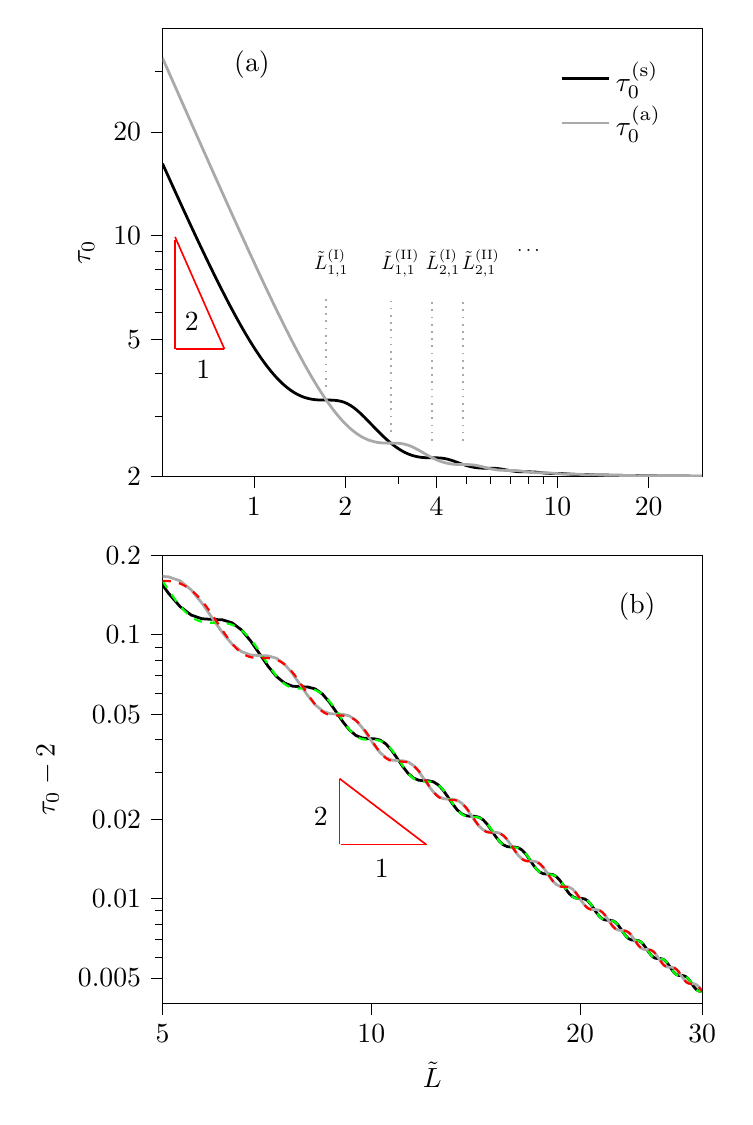
\begin{tikzpicture}

\definecolor{darkgray}{RGB}{169,169,169}
\definecolor{darkgray176}{RGB}{176,176,176}

\begin{groupplot}[group style={group size=1 by 2}]
\nextgroupplot[
log ticks with fixed point, %afegit a ma
ytick={2,5,10,20}, %afegit a ma
minor ytick={3,4,6,7,8,9,30}, %afegit a ma
xtick={1,2,4,10,20}, %afegit a ma
minor xtick={3,5,6,7,8,9}, %afegit a ma
legend cell align={left},
legend style={fill opacity=0.8, draw opacity=1, text opacity=1, at={(0.95,0.95)}, draw=none},
log basis x={10},
log basis y={10},
tick align=outside,
tick pos=left,
x grid style={darkgray176},
xmin=0.5, xmax=30,
xmode=log,
xtick style={color=black},
y grid style={darkgray176},
ylabel={\(\displaystyle \tau_0\)},
ymin=2, ymax=40,
ymode=log,
ytick style={color=black}
]
\addplot [line width=1pt, black]
table {%
0.5 16.1873971654469
0.52 14.9955692399881
0.54 13.9359578067725
0.56 12.990098801246
0.58 12.1426554171925
0.6 11.3808033050015
0.62 10.6937522863086
0.64 10.0723710081298
0.66 9.50888997247584
0.68 8.99666478023081
0.7 8.5299860288148
0.72 8.10392564441343
0.74 7.71421188049086
0.76 7.35712702908208
0.78 7.02942324700963
0.8 6.72825292030247
0.82 6.45111076531796
0.84 6.19578545798727
0.86 5.96031903929238
0.88 5.74297269919318
0.9 5.54219781754253
0.92 5.35661135744574
0.94 5.18497487778882
0.96 5.02617656762402
0.98 4.87921581360383
1 4.7431898986731
1.02 4.61728250035039
1.04 4.50075371369173
1.06 4.39293137017771
1.08 4.29320346143936
1.1 4.20101150761725
1.12 4.11584473555358
1.14 4.03723495299532
1.16 3.96475202236877
1.18 3.89799985213701
1.2 3.83661283580419
1.22 3.78025267871402
1.24 3.72860556125143
1.26 3.68137959417931
1.28 3.63830252785762
1.3 3.59911968219061
1.32 3.56359206848789
1.34 3.53149467813925
1.36 3.50261491620545
1.38 3.47675116081516
1.4 3.45371143172086
1.42 3.43331215358275
1.44 3.41537700159799
1.46 3.3997358190469
1.48 3.38622359826666
1.5 3.37467951856636
1.52 3.36494603675231
1.54 3.3568680283309
1.56 3.35029198019372
1.58 3.34506523876448
1.6 3.34103532128661
1.62 3.33804930222195
1.64 3.3359532916368
1.66 3.33459202791697
1.68 3.33380861300257
1.7 3.33344442421368
1.72 3.33333924205736
1.74 3.33333163727308
1.76 3.33325966156223
1.78 3.33296188341514
1.8 3.33227880145649
1.82 3.33105465109557
1.84 3.32913959480442
1.86 3.32639225195012
1.88 3.32268248241901
1.9 3.31789429320694
1.92 3.31192869502812
1.94 3.30470630493384
1.96 3.29616947940436
1.98 3.28628377701964
2 3.27503859310346
2.02 3.2624468773298
2.04 3.24854392990884
2.06 3.23338535917859
2.08 3.21704435882347
2.1 3.19960851481965
2.12 3.18117637431073
2.14 3.1618540010999
2.16 3.14175171093658
2.18 3.12098113314365
2.2 3.09965269289594
2.22 3.077873558702
2.24 3.05574605784447
2.26 3.03336653137667
2.28 3.01082458008055
2.3 2.98820264230395
2.32 2.96557584174608
2.34 2.94301204578965
2.36 2.92057208083387
2.38 2.89831005861214
2.4 2.87627377548193
2.42 2.85450515436404
2.44 2.83304070592929
2.46 2.81191199157288
2.48 2.79114607563233
2.5 2.77076595824993
2.52 2.75079098336004
2.54 2.73123721862548
2.56 2.7121178058846
2.58 2.69344328192268
2.6 2.6752218702529
2.62 2.65745974517188
2.64 2.64016126971595
2.66 2.62332920934319
2.68 2.60696492324937
2.7 2.59106853522729
2.72 2.57563908592478
2.74 2.56067466826703
2.76 2.54617254769756
2.78 2.53212926876976
2.8 2.51854074949485
2.82 2.50540236472681
2.84 2.49270901974457
2.86 2.48045521507725
2.88 2.46863510351212
2.9 2.45724254012673
2.92 2.44627112609667
2.94 2.43571424694899
2.96 2.42556510585734
2.98 2.41581675250848
3 2.40646210800992
3.02 2.39749398625543
3.04 2.38890511211673
3.06 2.38068813678772
3.08 2.37283565056923
3.1 2.36534019334859
3.12 2.35819426299837
3.14 2.35139032189195
3.16 2.34492080170994
3.18 2.33877810669068
3.2 2.33295461545946
3.22 2.32744268155518
3.24 2.32223463275883
3.26 2.31732276931604
3.28 2.31269936113546
3.3 2.30835664403593
3.32 2.30428681510831
3.34 2.30048202725224
3.36 2.29693438294397
3.38 2.29363592728941
3.4 2.29057864041559
3.42 2.28775442925503
3.44 2.28515511878069
3.46 2.2827724427543
3.48 2.28059803405852
3.5 2.27862341469332
3.52 2.27683998553009
3.54 2.27523901593273
3.56 2.27381163337438
3.58 2.27254881320159
3.6 2.27144136872421
3.62 2.27047994184068
3.64 2.2696549944431
3.66 2.26895680088598
3.68 2.26837544184565
3.7 2.26790079994381
3.72 2.26752255755767
3.74 2.26723019728936
3.76 2.2670130056165
3.78 2.26686008029186
3.8 2.26676034209918
3.82 2.2667025516004
3.84 2.26667533152177
3.86 2.26666719541617
3.88 2.2666665832009
3.9 2.26666190409579
3.92 2.26664158737033
3.94 2.26659414114375
3.96 2.26650821926418
3.98 2.26637269602117
4 2.26617674812126
4.02 2.26590994298664
4.04 2.26556233203532
4.06 2.26512454718659
4.08 2.26458789843406
4.1 2.26394446997055
4.12 2.26318721206893
4.14 2.26231002575388
4.16 2.26130783727222
4.18 2.26017665950526
4.2 2.25891363777606
4.22 2.25751707798195
4.24 2.25598645560758
4.26 2.2543224049088
4.28 2.25252668835411
4.3 2.25060214721103
4.32 2.24855263491284
4.34 2.24638293548235
4.36 2.24409866978402
4.38 2.24170619269595
4.4 2.23921248442968
4.42 2.23662503918596
4.44 2.23395175413835
4.46 2.23120082141602
4.48 2.22838062534809
4.5 2.22549964677324
4.52 2.22256637574402
4.54 2.21958923349715
4.56 2.21657650414071
4.58 2.21353627614284
4.6 2.21047639340351
4.62 2.20740441545301
4.64 2.2043275861464
4.66 2.20125281010682
4.68 2.19818663610416
4.7 2.1951352465315
4.72 2.19210445215
4.74 2.18909969130661
4.76 2.1861260328796
4.78 2.18318818226912
4.8 2.18029048981813
4.82 2.17743696111904
4.84 2.17463126873094
4.86 2.17187676489802
4.88 2.16917649492177
4.9 2.16653321089553
4.92 2.16394938556033
4.94 2.16142722608587
4.96 2.15896868761904
4.98 2.15657548647618
5 2.15424911288377
5.02 2.15199084319659
5.04 2.14980175154224
5.06 2.147682720858
5.08 2.14563445329937
5.1 2.14365748001086
5.12 2.14175217025838
5.14 2.1399187399295
5.16 2.13815725941347
5.18 2.13646766087674
5.2 2.13484974495311
5.22 2.1333031868696
5.24 2.131827542031
5.26 2.13042225108692
5.28 2.12908664450602
5.3 2.12781994668234
5.32 2.1266212795992
5.34 2.12548966607597
5.36 2.12442403262355
5.38 2.12342321193424
5.4 2.1224859450324
5.42 2.12161088311237
5.44 2.12079658909131
5.46 2.1200415389051
5.48 2.11934412257704
5.5 2.11870264509048
5.52 2.1181153270986
5.54 2.11758030550663
5.56 2.11709563396506
5.58 2.1166592833148
5.6 2.11626914202972
5.62 2.1159230167054
5.64 2.11561863264758
5.66 2.11535363461882
5.68 2.11512558780664
5.7 2.11493197908206
5.72 2.1147702186227
5.74 2.11463764197988
5.76 2.11453151267443
5.78 2.11444902540993
5.8 2.11438730999594
5.82 2.11434343607585
5.84 2.11431441875434
5.86 2.1142972252177
5.88 2.11428878243573
5.9 2.11428598602576
5.92 2.11428571034752
5.94 2.11428481988129
5.96 2.11428018192038
5.98 2.11426868058257
6 2.11424723211327
6.02 2.11421280141656
6.04 2.11416241970824
6.06 2.11409320314003
6.08 2.11400237219614
6.1 2.11388727161493
6.12 2.11374539054114
6.14 2.11357438257128
6.16 2.11337208531778
6.18 2.113136539091
6.2 2.11286600428265
6.22 2.11255897703378
6.24 2.112214202786
6.26 2.11183068734652
6.28 2.11140770514672
6.3 2.11094480443817
6.32 2.11044180924731
6.34 2.10989881799695
6.36 2.1093161987953
6.38 2.10869458148667
6.4 2.10803484664758
6.42 2.10733811179369
6.44 2.10660571513187
6.46 2.10583919724653
6.48 2.10504028114617
6.5 2.10421085111581
6.52 2.1033529308232
6.54 2.10246866111246
6.56 2.10156027789147
6.58 2.10063009047997
6.6 2.09968046073861
6.62 2.0987137832465
6.64 2.09773246674086
6.66 2.09673891697788
6.68 2.09573552112251
6.7 2.09472463372725
6.72 2.09370856431782
6.74 2.09268956656764
6.76 2.09166982901247
6.78 2.09065146723346
6.8 2.08963651741847
6.82 2.08862693119917
6.84 2.08762457165363
6.86 2.08663121036043
6.88 2.08564852538979
6.9 2.08467810011975
6.92 2.08372142276967
6.94 2.08277988654942
6.96 2.08185479032943
6.98 2.08094733974443
7 2.08005864865176
7.02 2.07918974087269
7.04 2.07834155215348
7.06 2.0775149322899
7.08 2.07671064736627
7.1 2.07592938206639
7.12 2.07517174202013
7.14 2.07443825615445
7.16 2.07372937902305
7.18 2.07304549309295
7.2 2.07238691097054
7.22 2.07175387755295
7.24 2.07114657209393
7.26 2.07056511017585
7.28 2.07000954558228
7.3 2.06947987206739
7.32 2.06897602502039
7.34 2.0684978830251
7.36 2.068045269316
7.38 2.06761795313356
7.4 2.06721565098299
7.42 2.06683802780162
7.44 2.06648469804133
7.46 2.06615522667345
7.48 2.0658491301246
7.5 2.06556587715331
7.52 2.06530488967781
7.54 2.06506554356717
7.56 2.06484716940859
7.58 2.06464905326516
7.6 2.06447043743968
7.62 2.06431052126128
7.64 2.06416846191315
7.66 2.0640433753209
7.68 2.06393433712261
7.7 2.0638403837428
7.72 2.06376051359411
7.74 2.06369368843145
7.76 2.06363883488448
7.78 2.06359484619516
7.8 2.06356058418743
7.82 2.06353488149637
7.84 2.06351654408356
7.86 2.06350435406449
7.88 2.0634970728722
7.9 2.06349344477845
7.92 2.06349220079073
7.94 2.06349206293846
7.96 2.06349174895635
7.98 2.06348997736599
8 2.06348547294887
8.02 2.06347697259496
8.04 2.0634632315006
8.06 2.06344302967882
8.08 2.06341517873328
8.1 2.06337852883498
8.12 2.06333197582926
8.14 2.06327446838874
8.16 2.06320501511775
8.18 2.06312269150485
8.2 2.06302664661306
8.22 2.06291610939365
8.24 2.06279039450801
8.26 2.06264890754462
8.28 2.0624911495242
8.3 2.06231672059589
8.32 2.0621253228407
8.34 2.06191676211515
8.36 2.06169094888722
8.38 2.06144789803842
8.4 2.06118772762824
8.42 2.06091065664047
8.44 2.06061700175315
8.46 2.06030717319493
8.48 2.05998166976947
8.5 2.0596410731449
8.52 2.05928604151786
8.54 2.05891730277006
8.56 2.05853564723963
8.58 2.05814192023065
8.6 2.05773701438111
8.62 2.05732186200387
8.64 2.05689742750632
8.66 2.05646469998426
8.68 2.0560246860727
8.7 2.0555784031241
8.72 2.05512687277048
8.74 2.05467111491328
8.76 2.05421214217159
8.78 2.05375095480828
8.8 2.05328853614237
8.82 2.05282584844685
8.84 2.05236382932324
8.86 2.05190338853719
8.88 2.05144540529446
8.9 2.05099072593215
8.92 2.0505401619976
8.94 2.05009448868486
8.96 2.04965444359811
8.98 2.04922072581101
9 2.04879399519105
9.02 2.04837487195922
9.04 2.0479639364564
9.06 2.0475617290893
9.08 2.04716875043073
9.1 2.04678546145073
9.12 2.04641228385709
9.14 2.04604960052567
9.16 2.04569775600298
9.18 2.04535705706525
9.2 2.04502777332013
9.22 2.04471013783883
9.24 2.04440434780807
9.26 2.04411056519291
9.28 2.04382891740275
9.3 2.04355949795427
9.32 2.04330236712615
9.34 2.04305755260169
9.36 2.04282505009644
9.38 2.04260482396885
9.4 2.04239680781304
9.42 2.0422009050335
9.44 2.04201698940235
9.46 2.04184490560068
9.48 2.04168446974609
9.5 2.04153546990932
9.52 2.04139766662363
9.54 2.04127079339101
9.56 2.04115455719039
9.58 2.04104863899319
9.6 2.04095269429266
9.62 2.04086635365359
9.64 2.04078922329019
9.66 2.04072088567994
9.68 2.04066090022218
9.7 2.04060880395057
9.72 2.04056411230911
9.74 2.04052632000159
9.76 2.04049490192502
9.78 2.04046931419737
9.8 2.0404489952903
9.82 2.04043336727724
9.84 2.04042183720701
9.86 2.04041379861241
9.88 2.04040863316249
9.9 2.04040571246615
9.92 2.04040440003294
9.94 2.04040405339549
9.96 2.04040402639546
9.98 2.04040367163249
10 2.04040234307249
10.02 2.04039939880854
10.04 2.04039420396355
10.06 2.0403861337203
10.08 2.04037457646003
10.1 2.0403589369866
10.12 2.04033863980881
10.14 2.04031313244968
10.16 2.04028188874712
10.18 2.04024441210757
10.2 2.04020023867119
10.22 2.04014894034506
10.24 2.04009012766023
10.26 2.04002345240803
10.28 2.0399486100127
10.3 2.03986534159939
10.32 2.03977343572052
10.34 2.03967272970808
10.36 2.03956311062558
10.38 2.03944451579972
10.4 2.03931693291978
10.42 2.03918039970043
10.44 2.03903500311193
10.46 2.0388808781898
10.48 2.03871820644361
10.5 2.03854721389205
10.52 2.03836816875732
10.54 2.03818137885735
10.56 2.0379871887386
10.58 2.03778597659468
10.6 2.03757815101798
10.62 2.03736414763166
10.64 2.03714442564844
10.66 2.03691946440108
10.68 2.03668975988617
10.7 2.03645582135981
10.72 2.03621816801938
10.74 2.03597732580122
10.76 2.03573382431942
10.78 2.03548819396626
10.8 2.03524096318993
10.82 2.03499265596125
10.84 2.03474378943646
10.86 2.03449487181971
10.88 2.03424640042555
10.9 2.0339988599386
10.92 2.03375272086533
10.94 2.03350843817075
10.96 2.03326645009117
10.98 2.03302717711321
11 2.03279102110787
11.02 2.03255836460865
11.04 2.03232957022162
11.06 2.03210498015605
11.08 2.03188491586383
11.1 2.03166967777649
11.12 2.03145954512915
11.14 2.03125477586096
11.16 2.03105560658255
11.18 2.03086225260161
11.2 2.03067490799822
11.22 2.03049374574249
11.24 2.03031891784783
11.26 2.03015055555358
11.28 2.02998876953189
11.3 2.02983365011387
11.32 2.02968526753138
11.34 2.02954367217064
11.36 2.02940889483526
11.38 2.02928094701629
11.4 2.02915982116764
11.42 2.02904549098589
11.44 2.02893791169373
11.46 2.028837020327
11.48 2.02874273602562
11.5 2.02865496032922
11.52 2.02857357747862
11.54 2.0284984547249
11.56 2.02842944264794
11.58 2.02836637548694
11.6 2.0283090714857
11.62 2.02825733325564
11.64 2.02821094816023
11.66 2.02816968872445
11.68 2.02813331307334
11.7 2.02810156540404
11.72 2.02807417649571
11.74 2.02805086426208
11.76 2.02803133435144
11.78 2.02801528079881
11.8 2.02800238673517
11.82 2.02799232515838
11.84 2.02798475977036
11.86 2.02797934588435
11.88 2.02797573140634
11.9 2.02797355789326
11.92 2.02797246169059
11.94 2.02797207515055
11.96 2.02797202793126
11.98 2.02797194837601
12 2.02797146497024
12.02 2.02797020787236
12.04 2.02796781051306
12.06 2.02796391125555
12.08 2.02795815510779
12.1 2.02795019547547
12.12 2.02793969594294
12.14 2.0279263320671
12.16 2.027909793168
12.18 2.02788978409793
12.2 2.02786602696988
12.22 2.02783826282502
12.24 2.02780625321849
12.26 2.02776978170246
12.28 2.02772865518596
12.3 2.0276827051515
12.32 2.02763178871012
12.34 2.02757578947822
12.36 2.0275146182617
12.38 2.02744821353588
12.4 2.02737654171264
12.42 2.02729959718953
12.44 2.02721740217927
12.46 2.0271300063215
12.48 2.02703748608243
12.5 2.02693994395122
12.52 2.02683750744536
12.54 2.02673032793997
12.56 2.02661857933852
12.58 2.0265024566043
12.6 2.02638217417361
12.62 2.02625796427245
12.64 2.0261300751589
12.66 2.02599876931333
12.68 2.02586432159812
12.7 2.0257270174073
12.72 2.02558715082571
12.74 2.02544502281504
12.76 2.02530093944283
12.78 2.02515521016833
12.8 2.02500814619693
12.82 2.02486005891305
12.84 2.02471125839926
12.86 2.0245620520473
12.88 2.02441274326503
12.9 2.02426363028157
12.92 2.02411500505136
12.94 2.02396715225642
12.96 2.02382034840512
12.98 2.02367486102474
13 2.02353094794397
13.02 2.02338885666151
13.04 2.02324882379569
13.06 2.0231110746103
13.08 2.02297582261136
13.1 2.02284326920932
13.12 2.0227136034415
13.14 2.02258700174941
13.16 2.02246362780583
13.18 2.02234363238675
13.2 2.0222271532835
13.22 2.02211431525065
13.24 2.02200522998565
13.26 2.02189999613642
13.28 2.02179869933353
13.3 2.02170141224385
13.32 2.021608194643
13.34 2.02151909350419
13.36 2.02143414310146
13.38 2.02135336512549
13.4 2.02127676881087
13.42 2.02120435107342
13.44 2.02113609665711
13.46 2.02107197828998
13.48 2.02101195684884
13.5 2.02095598153304
13.52 2.02090399004751
13.54 2.02085590879579
13.56 2.02081165308391
13.58 2.02077112733626
13.6 2.02073422532476
13.62 2.02070083041283
13.64 2.02067081581605
13.66 2.02064404488129
13.68 2.02062037138639
13.7 2.0205996398627
13.72 2.02058168594279
13.74 2.02056633673552
13.76 2.02055341123127
13.78 2.02054272073946
13.8 2.02053406936091
13.82 2.02052725449734
13.84 2.02052206740017
13.86 2.02051829376049
13.88 2.02051571434205
13.9 2.02051410565836
13.92 2.02051324069495
13.94 2.02051288967714
13.96 2.02051282088309
13.98 2.02051280150121
14 2.02051259853043
14.02 2.02051197972079
14.04 2.02051071455111
14.06 2.02050857523941
14.08 2.02050533778108
14.1 2.0205007830084
14.12 2.02049469766453
14.14 2.02048687548367
14.16 2.02047711826876
14.18 2.02046523695678
14.2 2.0204510526615
14.22 2.02043439768271
14.24 2.02041511647091
14.26 2.0203930665361
14.28 2.02036811928954
14.3 2.02034016080772
14.32 2.02030909250827
14.34 2.02027483172851
14.36 2.02023731219833
14.38 2.02019648440038
14.4 2.02015231581211
14.42 2.02010479102581
14.44 2.02005391174441
14.46 2.01999969665302
14.48 2.01994218116742
14.5 2.01988141706321
14.52 2.01981747199045
14.54 2.01975042888068
14.56 2.01968038525435
14.58 2.01960745243807
14.6 2.01953175470203
14.62 2.0194534283288
14.64 2.01937262062502
14.66 2.01928948888803
14.68 2.01920419933918
14.7 2.01911692603558
14.72 2.01902784977152
14.74 2.01893715698019
14.76 2.01884503864552
14.78 2.01875168923318
14.8 2.01865730564873
14.82 2.01856208622993
14.84 2.01846622977911
14.86 2.01836993464061
14.88 2.01827339782701
14.9 2.0181768141972
14.92 2.01808037568815
14.94 2.0179842706016
14.96 2.01788868294602
14.98 2.01779379183348
15 2.01769977093064
15.02 2.01760678796233
15.04 2.01751500426602
15.06 2.01742457439502
15.08 2.01733564576796
15.1 2.01724835836199
15.12 2.01716284444708
15.14 2.01707922835851
15.16 2.01699762630492
15.18 2.01691814620912
15.2 2.01684088757894
15.22 2.01676594140566
15.24 2.01669339008745
15.26 2.01662330737565
15.28 2.01655575834162
15.3 2.0164907993623
15.32 2.01642847812263
15.34 2.01636883363329
15.36 2.01631189626232
15.38 2.01625768777942
15.4 2.01620622141191
15.42 2.01615750191156
15.44 2.01611152563164
15.46 2.01606828061364
15.48 2.01602774668361
15.5 2.01598989555776
15.52 2.01595469095765
15.54 2.01592208873497
15.56 2.01589203700652
15.58 2.01586447629978
15.6 2.0158393397098
15.62 2.01581655306832
15.64 2.0157960351258
15.66 2.01577769774781
15.68 2.01576144612642
15.7 2.0157471790083
15.72 2.01573478894034
15.74 2.01572416253457
15.76 2.01571518075322
15.78 2.0157077192157
15.8 2.01570164852845
15.82 2.01569683463906
15.84 2.01569313921568
15.86 2.01569042005278
15.88 2.01568853150394
15.9 2.01568732494235
15.92 2.0156866492493
15.94 2.01568635133056
15.96 2.01568627666048
15.98 2.01568626985293
16 2.0156861752579
16.02 2.01568583758215
16.04 2.01568510253175
16.06 2.01568381747376
16.08 2.0156818321139
16.1 2.01567899918634
16.12 2.01567517515137
16.14 2.01567022089607
16.16 2.01566400243267
16.18 2.01565639158883
16.2 2.01564726668376
16.22 2.01563651318377
16.24 2.01562402433066
16.26 2.01560970173634
16.28 2.01559345593697
16.3 2.01557520690043
16.32 2.01555488448069
16.34 2.01553242881371
16.36 2.01550779064958
16.38 2.01548093161658
16.4 2.01545182441358
16.42 2.01542045292801
16.44 2.01538681227775
16.46 2.01535090877614
16.48 2.01531275982055
16.5 2.01527239370568
16.52 2.0152298493642
16.54 2.01518517603784
16.56 2.01513843288323
16.58 2.0150896885175
16.6 2.0150390205092
16.62 2.01498651482087
16.64 2.01493226520961
16.66 2.01487637259291
16.68 2.01481894438634
16.7 2.01476009382033
16.72 2.01469993924296
16.74 2.01463860341519
16.76 2.01457621280504
16.78 2.01451289688654
16.8 2.01444878744885
16.82 2.01438401792037
16.84 2.01431872271232
16.86 2.01425303658527
16.88 2.01418709404197
16.9 2.01412102874883
16.92 2.01405497298819
16.94 2.01398905714277
16.96 2.01392340921322
16.98 2.01385815436932
17 2.01379341453496
17.02 2.01372930800651
17.04 2.01366594910416
17.06 2.01360344785519
17.08 2.01354190970835
17.1 2.01348143527788
17.12 2.01342212011595
17.14 2.01336405451195
17.16 2.01330732331725
17.18 2.01325200579368
17.2 2.01319817548437
17.22 2.01314590010524
17.24 2.01309524145582
17.26 2.01304625534779
17.28 2.0129989915501
17.3 2.01295349374918
17.32 2.01290979952326
17.34 2.01286794032956
17.36 2.01282794150361
17.38 2.01278982226967
17.4 2.01275359576157
17.42 2.01271926905345
17.44 2.01268684319985
17.46 2.01265631328473
17.48 2.01262766847925
17.5 2.01260089210818
17.52 2.01257596172477
17.54 2.0125528491943
17.56 2.01253152078649
17.58 2.01251193727683
17.6 2.01249405405758
17.62 2.01247782125843
17.64 2.01246318387777
17.66 2.01245008192483
17.68 2.01243845057359
17.7 2.01242822032901
17.72 2.01241931720633
17.74 2.01241166292426
17.76 2.0124051751128
17.78 2.01239976753633
17.8 2.01239535033288
17.82 2.01239183027006
17.84 2.01238911101837
17.86 2.01238709344232
17.88 2.01238567590973
17.9 2.01238475461955
17.92 2.01238422394804
17.94 2.01238397681341
17.96 2.01238390505837
17.98 2.01238389985004
18 2.01238385209638
18.02 2.01238365287778
18.04 2.01238319389256
18.06 2.01238236791429
18.08 2.01238106925895
18.1 2.01237919425944
18.12 2.01237664174451
18.14 2.01237331351904
18.16 2.01236911484236
18.18 2.01236395490071
18.2 2.01235774727021
18.22 2.01235041036605
18.24 2.01234186787392
18.26 2.01233204915933
18.28 2.01232088965073
18.3 2.01230833119232
18.32 2.01229432236258
18.34 2.01227881875502
18.36 2.0122617832177
18.38 2.01224318604875
18.4 2.01222300514527
18.42 2.012201226104
18.44 2.01217784227221
18.46 2.01215285474816
18.48 2.01212627233113
18.5 2.01209811142149
18.52 2.01206839587206
18.54 2.01203715679253
18.56 2.01200443230917
18.58 2.01197026728298
18.6 2.01193471298923
18.62 2.01189782676237
18.64 2.01185967161016
18.66 2.01182031580127
18.68 2.01177983243074
18.7 2.01173829896771
18.72 2.01169579678986
18.74 2.0116524107088
18.76 2.01160822849081
18.78 2.0115633403766
18.8 2.01151783860408
18.82 2.01147181693743
18.84 2.01142537020559
18.86 2.01137859385296
18.88 2.0113315835047
18.9 2.01128443454862
18.92 2.01123724173551
18.94 2.01119009879904
18.96 2.01114309809644
18.98 2.01109633027058
19 2.01104988393391
19.02 2.01100384537446
19.04 2.01095829828372
19.06 2.01091332350637
19.08 2.01086899881128
19.1 2.01082539868315
19.12 2.01078259413431
19.14 2.01074065253576
19.16 2.01069963746655
19.18 2.01065960858077
19.2 2.01062062149113
19.22 2.01058272766816
19.24 2.01054597435423
19.26 2.01051040449135
19.28 2.01047605666202
19.3 2.01044296504217
19.32 2.01041115936551
19.34 2.01038066489854
19.36 2.01035150242556
19.38 2.01032368824311
19.4 2.01029723416334
19.42 2.01027214752579
19.44 2.01024843121737
19.46 2.01022608370011
19.48 2.01020509904651
19.5 2.01018546698243
19.52 2.01016717293729
19.54 2.01015019810179
19.56 2.01013451949307
19.58 2.01012011002747
19.6 2.0101069386012
19.62 2.01009497017904
19.64 2.01008416589146
19.66 2.01007448314042
19.68 2.01006587571442
19.7 2.01005829391298
19.72 2.0100516846812
19.74 2.01004599175463
19.76 2.01004115581515
19.78 2.01003711465807
19.8 2.01003380337106
19.82 2.01003115452496
19.84 2.01002909837726
19.86 2.0100275630881
19.88 2.01002647494912
19.9 2.01002575862517
19.92 2.01002533740895
19.94 2.01002513348816
19.96 2.01002506822507
19.98 2.01002506244779
20 2.01002503675271
20.02 2.01002491181709
20.04 2.0100246087208
20.06 2.0100240492759
20.08 2.01002315636252
20.1 2.0100218542693
20.12 2.01002006903653
20.14 2.01001772879974
20.16 2.01001476413159
20.18 2.01001110837934
20.2 2.01000669799558
20.22 2.01000147285921
20.24 2.00999537658414
20.26 2.00998835681264
20.28 2.0099803654908
20.3 2.00997135912316
20.32 2.00996129900398
20.34 2.00995015142273
20.36 2.00993788784142
20.38 2.00992448504197
20.4 2.00990992524172
20.42 2.00989419617592
20.44 2.00987729114605
20.46 2.00985920903353
20.48 2.00983995427846
20.5 2.00981953682375
20.52 2.00979797202518
20.54 2.00977528052845
20.56 2.00975148811466
20.58 2.00972662551578
20.6 2.00970072820249
20.62 2.00967383614635
20.64 2.0096459935592
20.66 2.0096172486122
20.68 2.00958765313766
20.7 2.00955726231637
20.72 2.0095261343535
20.74 2.009494330146
20.76 2.00946191294428
20.78 2.00942894801109
20.8 2.00939550228008
20.82 2.00936164401658
20.84 2.00932744248285
20.86 2.0092929676098
20.88 2.00925828967717
20.9 2.00922347900353
20.92 2.00918860564772
20.94 2.00915373912271
20.96 2.00911894812299
20.98 2.0090843002658
21 2.00904986184736
21.02 2.00901569761388
21.04 2.00898187054769
21.06 2.00894844166864
21.08 2.00891546985048
21.1 2.00888301165207
21.12 2.00885112116309
21.14 2.00881984986386
21.16 2.0087892464987
21.18 2.00875935696247
21.2 2.00873022419965
21.22 2.00870188811533
21.24 2.00867438549772
21.26 2.00864774995136
21.28 2.00862201184063
21.3 2.00859719824305
21.32 2.00857333291162
21.34 2.00855043624596
21.36 2.00852852527168
21.38 2.00850761362761
21.4 2.00848771156041
21.42 2.0084688259265
21.44 2.00845096020072
21.46 2.00843411449176
21.48 2.00841828556409
21.5 2.00840346686624
21.52 2.0083896485654
21.54 2.00837681758837
21.56 2.00836495766876
21.58 2.00835404940067
21.6 2.00834407029878
21.62 2.00833499486516
21.64 2.00832679466293
21.66 2.00831943839687
21.68 2.00831289200144
21.7 2.00830711873622
21.72 2.00830207928926
21.74 2.00829773188843
21.76 2.00829403242112
21.78 2.00829093456259
21.8 2.00828838991311
21.82 2.00828634814415
21.84 2.00828475715379
21.86 2.00828356323147
21.88 2.0082827112321
21.9 2.00828214475957
21.92 2.00828180635942
21.94 2.00828163772076
21.96 2.00828157988672
21.98 2.00828157347343
22 2.00828155889672
22.02 2.00828147660586
22.04 2.00828126732374
22.06 2.00828087229229
22.08 2.00828023352216
22.1 2.00827929404539
22.12 2.00827799816966
22.14 2.00827629173267
22.16 2.00827412235485
22.18 2.00827143968891
22.2 2.00826819566414
22.22 2.00826434472367
22.24 2.00825984405278
22.26 2.00825465379619
22.28 2.00824873726247
22.3 2.00824206111358
22.32 2.00823459553783
22.34 2.00822631440433
22.36 2.00821719539758
22.38 2.00820722013063
22.4 2.00819637423561
22.42 2.00818464743073
22.44 2.00817203356289
22.46 2.00815853062553
22.48 2.00814414075136
22.5 2.00812887018023
22.52 2.0081127292023
22.54 2.00809573207723
22.56 2.00807789693026
22.58 2.00805924562625
22.6 2.00803980362306
22.62 2.00801959980583
22.64 2.00799866630383
22.66 2.00797703829169
22.68 2.00795475377703
22.7 2.0079318533765
22.72 2.0079083800822
22.74 2.00788437902062
22.76 2.00785989720613
22.78 2.00783498329093
22.8 2.00780968731345
22.82 2.00778406044692
22.84 2.00775815474985
22.86 2.00773202291999
22.88 2.00770571805305
22.9 2.00767929340761
22.92 2.00765280217717
22.94 2.00762629727043
22.96 2.00759983110051
22.98 2.0075734553836
23 2.00754722094803
23.02 2.00752117755351
23.04 2.00749537372135
23.06 2.00746985657525
23.08 2.00744467169328
23.1 2.00741986297056
23.12 2.0073954724926
23.14 2.00737154041929
23.16 2.00734810487901
23.18 2.00732520187284
23.2 2.00730286518828
23.22 2.00728112632235
23.24 2.00726001441352
23.26 2.00723955618231
23.28 2.00721977587987
23.3 2.00720069524454
23.32 2.00718233346578
23.34 2.00716470715517
23.36 2.00714783032428
23.38 2.00713171436902
23.4 2.00711636806021
23.42 2.00710179754023
23.44 2.00708800632541
23.46 2.00707499531413
23.48 2.0070627628004
23.5 2.00705130449296
23.52 2.00704061353957
23.54 2.00703068055682
23.56 2.00702149366516
23.58 2.00701303852936
23.6 2.00700529840431
23.62 2.00699825418649
23.64 2.00699188447089
23.66 2.00698616561386
23.68 2.00698107180169
23.7 2.00697657512542
23.72 2.00697264566174
23.74 2.00696925156035
23.76 2.00696635913784
23.78 2.00696393297832
23.8 2.00696193604084
23.82 2.00696032977382
23.84 2.00695907423638
23.86 2.00695812822694
23.88 2.00695744941877
23.9 2.00695699450256
23.92 2.00695671933594
23.94 2.00695657909964
23.96 2.00695652846018
23.98 2.00695652173856
24 2.00695651308468
24.02 2.00695645665685
24.04 2.00695630680581
24.06 2.00695601826253
24.08 2.00695554632886
24.1 2.00695484707031
24.12 2.00695387750971
24.14 2.00695259582077
24.16 2.00695096152025
24.18 2.00694893565755
24.2 2.00694648100033
24.22 2.00694356221476
24.24 2.00694014603909
24.26 2.00693620144893
24.28 2.00693169981303
24.3 2.00692661503811
24.32 2.0069209237013
24.34 2.0069146051691
24.36 2.00690764170166
24.38 2.00690001854128
24.4 2.00689172398427
24.42 2.00688274943548
24.44 2.0068730894449
24.46 2.00686274172585
24.48 2.00685170715471
24.5 2.00683998975212
24.52 2.0068275966458
24.54 2.00681453801547
24.56 2.00680082702037
24.58 2.00678647971014
24.6 2.00677151492001
24.62 2.00675595415133
24.64 2.00673982143859
24.66 2.00672314320432
24.68 2.00670594810307
24.7 2.00668826685615
24.72 2.00667013207828
24.74 2.00665157809801
24.76 2.00663264077302
24.78 2.00661335730201
24.8 2.00659376603453
24.82 2.00657390628
24.84 2.00655381811732
24.86 2.00653354220616
24.88 2.00651311960116
24.9 2.00649259156977
24.92 2.00647199941495
24.94 2.00645138430322
24.96 2.00643078709894
24.98 2.00641024820512
25 2.00638980741158
25.02 2.0063695037505
25.04 2.00634937535978
25.06 2.00632945935434
25.08 2.00630979170553
25.1 2.00629040712862
25.12 2.00627133897838
25.14 2.00625261915262
25.16 2.00623427800366
25.18 2.00621634425744
25.2 2.00619884494021
25.22 2.00618180531245
25.24 2.00616524880991
25.26 2.00614919699143
25.28 2.00613366949334
25.3 2.00611868399021
25.32 2.00610425616161
25.34 2.00609039966478
25.36 2.00607712611293
25.38 2.00606444505886
25.4 2.00605236398395
25.42 2.00604088829209
25.44 2.00603002130856
25.46 2.00601976428376
25.48 2.00601011640152
25.5 2.00600107479213
25.52 2.00599263454981
25.54 2.00598478875482
25.56 2.0059775285
25.58 2.00597084292191
25.6 2.00596471923643
25.62 2.00595914277912
25.64 2.00595409705012
25.66 2.00594956376387
25.68 2.00594552290371
25.7 2.00594195278136
25.72 2.0059388301015
25.74 2.00593613003148
25.76 2.00593382627628
25.78 2.00593189115879
25.8 2.00593029570556
25.82 2.00592900973793
25.84 2.00592800196873
25.86 2.00592724010446
25.88 2.00592669095287
25.9 2.00592632053608
25.92 2.00592609420881
25.94 2.00592597678184
25.96 2.00592593265022
25.98 2.00592592592626
26 2.00592592057637
26.02 2.00592588056216
26.04 2.00592576998451
26.06 2.00592555323049
26.08 2.00592519512235
26.1 2.0059246610679
26.12 2.00592391721147
26.14 2.0059229305846
26.16 2.0059216692556
26.18 2.00592010247698
26.2 2.00591820082972
26.22 2.00591593636345
26.24 2.00591328273139
26.26 2.00591021531898
26.28 2.0059067113653
26.3 2.00590275007605
26.32 2.00589831272724
26.34 2.00589338275865
26.36 2.00588794585605
26.38 2.00588199002167
26.4 2.00587550563195
26.42 2.00586848548227
26.44 2.00586092481794
26.46 2.00585282135145
26.48 2.00584417526555
26.5 2.00583498920221
26.52 2.00582526823766
26.54 2.00581501984361
26.56 2.00580425383518
26.58 2.00579298230593
26.6 2.00578121955073
26.62 2.00576898197719
26.64 2.00575628800643
26.66 2.00574315796426
26.68 2.00572961396361
26.7 2.00571567977939
26.72 2.00570138071674
26.74 2.00568674347386
26.76 2.00567179600054
26.78 2.00565656735333
26.8 2.00564108754864
26.82 2.00562538741462
26.84 2.00560949844283
26.86 2.00559345264075
26.88 2.00557728238583
26.9 2.0055610202819
26.92 2.00554469901873
26.94 2.00552835123547
26.96 2.00551200938794
26.98 2.00549570562123
27 2.00547947164714
27.02 2.00546333862726
27.04 2.0054473370617
27.06 2.005431496684
27.08 2.00541584636175
27.1 2.00540041400387
27.12 2.0053852264737
27.14 2.00537030950848
27.16 2.00535568764489
27.18 2.00534138415067
27.2 2.00532742096218
27.22 2.00531381862778
27.24 2.00530059625689
27.26 2.00528777147445
27.28 2.00527536038092
27.3 2.00526337751724
27.32 2.00525183583494
27.34 2.00524074667102
27.36 2.00523011972753
27.38 2.00521996305569
27.4 2.0052102830444
27.42 2.00520108441302
27.44 2.0051923702083
27.46 2.00518414180544
27.48 2.00517639891302
27.5 2.00516913958201
27.52 2.00516236021854
27.54 2.00515605560056
27.56 2.00515021889841
27.58 2.00514484169909
27.6 2.00513991403455
27.62 2.00513542441376
27.64 2.00513135985871
27.66 2.00512770594448
27.68 2.00512444684323
27.7 2.00512156537233
27.72 2.00511904304668
27.74 2.00511686013517
27.76 2.00511499572147
27.78 2.00511342776914
27.8 2.00511213319105
27.82 2.00511108792321
27.84 2.00511026700307
27.86 2.00510964465194
27.88 2.00510919436202
27.9 2.00510888898753
27.92 2.00510870083978
27.94 2.00510860178655
27.96 2.00510856335513
27.98 2.00510855683856
28 2.00510855340553
28.02 2.00510852421302
28.04 2.00510844052123
28.06 2.00510827381083
28.08 2.00510799590153
28.1 2.00510757907172
28.12 2.00510699617839
28.14 2.00510622077678
28.16 2.00510522723906
28.18 2.00510399087119
28.2 2.00510248802737
28.22 2.00510069622105
28.24 2.005098594232
28.26 2.00509616220835
28.28 2.00509338176295
28.3 2.00509023606326
28.32 2.00508670991394
28.34 2.00508278983153
28.36 2.00507846411047
28.38 2.00507372287996
28.4 2.00506855815097
28.42 2.00506296385319
28.44 2.00505693586139
28.46 2.00505047201099
28.48 2.00504357210274
28.5 2.00503623789641
28.52 2.00502847309353
28.54 2.00502028330948
28.56 2.005011676035
28.58 2.00500266058768
28.6 2.00499324805375
28.62 2.00498345122085
28.64 2.00497328450227
28.66 2.00496276385339
28.68 2.00495190668118
28.7 2.00494073174729
28.72 2.00492925906585
28.74 2.00491750979653
28.76 2.00490550613394
28.78 2.00489327119398
28.8 2.0048808288982
28.82 2.00486820385675
28.84 2.00485542125086
28.86 2.00484250671544
28.88 2.00482948622258
28.9 2.00481638596657
28.92 2.0048032322509
28.94 2.00479005137812
28.96 2.00477686954227
28.98 2.00476371272536
29 2.00475060659725
29.02 2.00473757641985
29.04 2.00472464695559
29.06 2.00471184238045
29.08 2.00469918620181
29.1 2.00468670118062
29.12 2.00467440925913
29.14 2.00466233149294
29.16 2.00465048798804
29.18 2.0046388978428
29.2 2.00462757909458
29.22 2.00461654867109
29.24 2.00460582234636
29.26 2.00459541470119
29.28 2.00458533908799
29.3 2.00457560759987
29.32 2.00456623104393
29.34 2.00455721891853
29.36 2.00454857939455
29.38 2.00454031930039
29.4 2.0045324441108
29.42 2.0045249579392
29.44 2.00451786353368
29.46 2.00451116227634
29.48 2.00450485418617
29.5 2.00449893792519
29.52 2.00449341080797
29.54 2.00448826881444
29.56 2.00448350660597
29.58 2.00447911754475
29.6 2.00447509371645
29.62 2.00447142595617
29.64 2.00446810387772
29.66 2.00446511590631
29.68 2.00446244931451
29.7 2.00446009026176
29.72 2.00445802383724
29.74 2.00445623410632
29.76 2.00445470416048
29.78 2.00445341617076
29.8 2.0044523514449
29.82 2.00445149048784
29.84 2.0044508130661
29.86 2.00445029827514
29.88 2.00444992461084
29.9 2.00444967004388
29.92 2.00444951209762
29.94 2.00444942792903
29.96 2.00444939441262
29.98 2.00444938822715
30 2.00444938594483
};
\addlegendentry{$\tau_0^{(\text{s})}$}
\addplot [line width=1pt, darkgray]
table {%
0.5 32.7828919351573
0.52 30.3176218724273
0.54 28.1217807262207
0.56 26.157597592197
0.58 24.3936993825357
0.6 22.8038531154049
0.62 21.3659874836861
0.64 20.0614250131859
0.66 18.8742745586187
0.68 17.7909469841802
0.7 16.7997662874843
0.72 15.890655261034
0.74 15.0548797994059
0.76 14.2848396729223
0.78 13.5738963619234
0.8 12.9162306347444
0.82 12.3067241384423
0.84 11.7408604842961
0.86 11.2146422444013
0.88 10.7245210001273
0.9 10.2673381485147
0.92 9.84027461648464
0.94 9.440807983139
0.96 9.06667578862161
0.98 8.71584403002105
1 8.38648002286545
1.02 8.0769289502634
1.04 7.78569353792596
1.06 7.51141638777685
1.08 7.25286458000155
1.1 7.00891621663488
1.12 6.7785486318439
1.14 6.56082803706986
1.16 6.35490040485055
1.18 6.15998342481031
1.2 5.97535939006908
1.22 5.80036889306039
1.24 5.63440522716911
1.26 5.47690940527796
1.28 5.32736571871509
1.3 5.18529777060464
1.32 5.0502649265521
1.34 4.92185913320324
1.36 4.79970206171225
1.38 4.68344253871684
1.4 4.57275423219106
1.42 4.46733356365277
1.44 4.36689782174188
1.46 4.27118345524344
1.48 4.17994452627742
1.5 4.09295130667355
1.52 4.00998900254642
1.54 3.93085659382474
1.56 3.85536577700625
1.58 3.78334000073589
1.6 3.71461358496685
1.62 3.64903091548267
1.64 3.58644570645423
1.66 3.52672032449344
1.68 3.46972516835998
1.7 3.41533809909102
1.72 3.36344391586582
1.74 3.31393387339747
1.76 3.26670523706961
1.78 3.22166087241408
1.8 3.17870886586148
1.82 3.13776217399556
1.84 3.0987382988092
1.86 3.06155898669748
1.88 3.02614994913545
1.9 2.99244060317878
1.92 2.96036383009478
1.94 2.9298557505839
1.96 2.90085551518827
1.98 2.8733051086062
2 2.84714916674165
2.02 2.82233480541631
2.04 2.7988114597609
2.06 2.77653073338216
2.08 2.7554462564738
2.1 2.7355135521047
2.12 2.71668990997589
2.14 2.69893426699067
2.16 2.68220709402981
2.18 2.66647028836723
2.2 2.6516870712006
2.22 2.63782188980733
2.24 2.6248403238696
2.26 2.61270899554247
2.28 2.60139548286827
2.3 2.59086823616799
2.32 2.58109649706714
2.34 2.57205021984068
2.36 2.5636999947893
2.38 2.55601697338814
2.4 2.54897279498128
2.42 2.54253951483014
2.44 2.53668953336431
2.46 2.53139552652965
2.48 2.5266303771826
2.5 2.52236710754396
2.52 2.51857881280088
2.54 2.51523859603567
2.56 2.51231950476638
2.58 2.50979446950901
2.6 2.50763624491763
2.62 2.50581735422854
2.64 2.50431003792933
2.66 2.50308620779414
2.68 2.50211740767187
2.7 2.50137478268093
2.72 2.50082905874767
2.74 2.50045053471385
2.76 2.50020908951885
2.78 2.50007420721139
2.8 2.50001502273648
2.82 2.50000039153947
2.84 2.4999989859877
2.86 2.4999794213812
2.88 2.4999104138558
2.9 2.49976097172364
2.92 2.499500620707
2.94 2.49909966207981
2.96 2.49852946094661
2.98 2.49776275981058
3 2.49677401031557
3.02 2.49553971374712
3.04 2.49403875875811
3.06 2.49225274308938
3.08 2.49016626504527
3.1 2.4877671703852
3.12 2.48504674126734
3.14 2.48199981597932
3.16 2.47862483132981
3.18 2.4749237835282
3.2 2.47090210780203
3.22 2.46656848147279
3.24 2.46193455929408
3.26 2.45701465317126
3.28 2.45182537064914
3.3 2.44638522764175
3.32 2.44071425079599
3.34 2.43483358377206
3.36 2.42876510982215
3.38 2.42253110063517
3.4 2.41615389877337
3.42 2.40965563840537
3.44 2.40305800663499
3.46 2.39638204566558
3.48 2.38964799439344
3.5 2.38287516680558
3.52 2.37608186374232
3.54 2.36928531412264
3.56 2.36250164155772
3.58 2.35574585232753
3.6 2.34903184090515
3.62 2.34237240952746
3.64 2.33577929868445
3.66 2.32926322579702
3.68 2.32283392974876
3.7 2.31650021931407
3.72 2.31027002387035
3.74 2.30415044509185
3.76 2.29814780859287
3.78 2.29226771472086
3.8 2.28651508789515
3.82 2.28089422405085
3.84 2.27540883588011
3.86 2.27006209567106
3.88 2.26485667563023
3.9 2.25979478564147
3.92 2.25487820846565
3.94 2.25010833242457
3.96 2.2454861816404
3.98 2.24101244392242
4 2.23668749640584
4.02 2.23251142905567
4.04 2.22848406615253
4.06 2.22460498587848
4.08 2.22087353811918
4.1 2.21728886059576
4.12 2.21384989343564
4.14 2.21055539228622
4.16 2.20740394006993
4.18 2.20439395747339
4.2 2.20152371225758
4.22 2.19879132747024
4.24 2.19619478863626
4.26 2.19373194999667
4.28 2.19140053986225
4.3 2.18919816514321
4.32 2.1871223151129
4.34 2.18517036446022
4.36 2.18333957568255
4.38 2.18162710086938
4.4 2.18002998292519
4.42 2.17854515627963
4.44 2.17716944713327
4.46 2.17589957328794
4.48 2.17473214361293
4.5 2.1736636572006
4.52 2.1726905022692
4.54 2.17180895487521
4.56 2.17101517750368
4.58 2.17030521761208
4.6 2.1696750062115
4.62 2.16912035657869
4.64 2.16863696320288
4.66 2.16822040108366
4.68 2.16786612550851
4.7 2.16756947245268
4.72 2.16732565975804
4.74 2.16712978926186
4.76 2.16697685006039
4.78 2.16686172310459
4.8 2.16677918733614
4.82 2.16672392757931
4.84 2.16669054440755
4.86 2.16667356620074
4.88 2.16666746359941
4.9 2.16666666654276
4.92 2.16666558404777
4.94 2.16665862684447
4.96 2.16664023292646
4.98 2.16660489600615
5 2.16654719677875
5.02 2.16646183680115
5.04 2.16634367468088
5.06 2.16618776415133
5.08 2.16598939348619
5.1 2.16574412558425
5.12 2.16544783794354
5.14 2.16509676164795
5.16 2.16468751841927
5.18 2.16421715475088
5.2 2.16368317214175
5.22 2.16308355249725
5.24 2.16241677785748
5.26 2.16168184375268
5.28 2.16087826566535
5.3 2.16000607828943
5.32 2.15906582750922
5.34 2.15805855525967
5.36 2.15698577766238
5.38 2.1558494570435
5.4 2.15465196862002
5.42 2.15339606277939
5.44 2.1520848239688
5.46 2.15072162725318
5.48 2.14931009359552
5.5 2.14785404486547
5.52 2.14635745949801
5.54 2.14482442961335
5.56 2.14325912027952
5.58 2.14166573146134
5.6 2.14004846305914
5.62 2.13841148330746
5.64 2.13675890068029
5.66 2.13509473934141
5.68 2.13342291808606
5.7 2.13174723264588
5.72 2.13007134117158
5.74 2.12839875266639
5.76 2.12673281811623
5.78 2.12507672404791
5.8 2.12343348824221
5.82 2.12180595733268
5.84 2.12019680603093
5.86 2.11860853773406
5.88 2.11704348628768
5.9 2.11550381869749
5.92 2.11399153860285
5.94 2.11250849034627
5.96 2.11105636349259
5.98 2.10963669767053
6 2.10825088762681
6.02 2.1069001883994
6.04 2.10558572053099
6.06 2.10430847525693
6.08 2.10306931961345
6.1 2.10186900142253
6.12 2.10070815411816
6.14 2.09958730138708
6.16 2.09850686160309
6.18 2.09746715204023
6.2 2.0964683928546
6.22 2.09551071082865
6.24 2.09459414287549
6.26 2.09371863930329
6.28 2.09288406684251
6.3 2.09209021144063
6.32 2.09133678083088
6.34 2.09062340688291
6.36 2.08994964774467
6.38 2.08931498978611
6.4 2.08871884935619
6.42 2.08816057436604
6.44 2.08763944571196
6.46 2.08715467855329
6.48 2.08670542346125
6.5 2.08629076745606
6.52 2.08590973495133
6.54 2.0855612886258
6.56 2.08524433024471
6.58 2.08495770145441
6.6 2.0847001845762
6.62 2.08447050342735
6.64 2.08426732419945
6.66 2.08408925642701
6.68 2.08393485408121
6.7 2.08380261682669
6.72 2.08369099148142
6.74 2.08359837372225
6.76 2.08352311008074
6.78 2.08346350027579
6.8 2.08341779993077
6.82 2.08338422372344
6.84 2.08336094901684
6.86 2.0833461200177
6.88 2.08333785250644
6.9 2.08333423917865
6.92 2.08333335563161
6.94 2.08333326702174
6.96 2.08333203540849
6.98 2.08332772778765
7 2.08331842480254
7.02 2.08330223010394
7.04 2.08327728031102
7.06 2.08324175550421
7.08 2.08319389015892
7.1 2.08313198440637
7.12 2.08305441548518
7.14 2.08295964922631
7.16 2.0828462513948
7.18 2.08271289869673
7.2 2.08255838924866
7.22 2.08238165230184
7.24 2.08218175701521
7.26 2.08195792007919
7.28 2.08170951200887
7.3 2.08143606194822
7.32 2.081137260857
7.34 2.08081296298776
7.36 2.08046318560085
7.38 2.08008810690766
7.4 2.07968806227653
7.42 2.07926353877804
7.44 2.07881516818622
7.46 2.0783437185868
7.48 2.07785008477295
7.5 2.07733527762998
7.52 2.07680041272532
7.54 2.07624669832572
7.56 2.07567542306291
7.58 2.07508794346069
7.6 2.07448567152274
7.62 2.07387006256182
7.64 2.07324260342891
7.66 2.07260480127679
7.68 2.071958172967
7.7 2.07130423520414
7.72 2.0706444954569
7.74 2.06998044370277
7.76 2.06931354501276
7.78 2.06864523297458
7.8 2.06797690393742
7.82 2.06730991204904
7.84 2.06664556504588
7.86 2.06598512074974
7.88 2.06532978421911
7.9 2.06468070550046
7.92 2.06403897792309
7.94 2.06340563688121
7.96 2.06278165904815
7.98 2.06216796196951
8 2.06156540398468
8.02 2.06097478442976
8.04 2.0603968440777
8.06 2.0598322657759
8.08 2.05928167524457
8.1 2.05874564200319
8.12 2.05822468039576
8.14 2.05771925068914
8.16 2.05722976022167
8.18 2.05675656458253
8.2 2.05629996880507
8.22 2.05586022855954
8.24 2.05543755133355
8.26 2.05503209759015
8.28 2.05464398189578
8.3 2.05427327401186
8.32 2.05391999994541
8.34 2.0535841429557
8.36 2.05326564451492
8.38 2.05296440522247
8.4 2.05268028567332
8.42 2.05241310728192
8.44 2.0521626530644
8.46 2.05192866838238
8.48 2.05171086165292
8.5 2.05150890502986
8.52 2.05132243506267
8.54 2.05115105333994
8.56 2.05099432712537
8.58 2.05085178999507
8.6 2.05072294248584
8.62 2.05060725276501
8.64 2.05050415733331
8.66 2.0504130617731
8.68 2.05033334155512
8.7 2.05026434291782
8.72 2.05020538383407
8.74 2.05015575508057
8.76 2.05011472142602
8.78 2.05008152295433
8.8 2.05005537653952
8.82 2.05003547748859
8.84 2.05002100136848
8.86 2.05001110603243
8.88 2.05000493385987
8.9 2.05000161422213
8.92 2.05000026618448
8.94 2.05000000145165
8.96 2.04999992756113
8.98 2.04999915132408
9 2.04999678250915
9.02 2.04999193775924
9.04 2.04998374472516
9.06 2.04997134639388
9.08 2.04995390558237
9.1 2.04993060956094
9.12 2.04990067476324
9.14 2.04986335153333
9.16 2.04981792885408
9.18 2.04976373899584
9.2 2.04970016202
9.22 2.04962663006934
9.24 2.04954263137559
9.26 2.04944771391535
9.28 2.04934148864815
9.3 2.04922363227481
9.32 2.04909388946125
9.34 2.04895207448114
9.36 2.04879807224137
9.38 2.04863183866557
9.4 2.04845340042389
9.42 2.04826285401031
9.44 2.04806036418182
9.46 2.04784616178682
9.48 2.04762054102204
9.5 2.0473838561675
9.52 2.04713651785856
9.54 2.0468789889605
9.56 2.04661178011645
9.58 2.04633544504209
9.6 2.04605057564112
9.62 2.04575779701435
9.64 2.04545776243224
9.66 2.04515114833578
9.68 2.04483864942524
9.7 2.0445209738892
9.72 2.0441988388192
9.74 2.04387296584767
9.76 2.04354407703906
9.78 2.04321289105678
9.8 2.04288011962147
9.82 2.04254646426956
9.84 2.04221261341539
9.86 2.04187923971481
9.88 2.04154699772406
9.9 2.04121652184385
9.92 2.04088842453574
9.94 2.04056329479582
9.96 2.04024169686885
9.98 2.03992416918498
10 2.03961122350093
10.02 2.03930334422683
10.04 2.03900098792055
10.06 2.03870458293158
10.08 2.03841452917734
10.1 2.0381311980356
10.12 2.03785493233768
10.14 2.03758604644826
10.16 2.0373248264186
10.18 2.03707153020131
10.2 2.03682638791574
10.22 2.03658960215435
10.24 2.0363613483215
10.26 2.03614177499696
10.28 2.03593100431776
10.3 2.03572913237271
10.32 2.03553622960487
10.34 2.03535234121822
10.36 2.03517748758547
10.38 2.03501166465475
10.4 2.03485484435356
10.42 2.0347069749893
10.44 2.03456798164592
10.46 2.03443776657725
10.48 2.03431620959793
10.5 2.03420316847345
10.52 2.03409847931149
10.54 2.034001956957
10.56 2.03391339539435
10.58 2.03383256816002
10.6 2.03375922877004
10.62 2.03369311116663
10.64 2.03363393018928
10.66 2.03358138207541
10.68 2.03353514499677
10.7 2.03349487963748
10.72 2.03346022982046
10.74 2.03343082318883
10.76 2.03340627194928
10.78 2.03338617368447
10.8 2.03337011224137
10.82 2.03335765870255
10.84 2.03334837244693
10.86 2.03334180230617
10.88 2.03333748782231
10.9 2.03333496061137
10.92 2.03333374583655
10.94 2.03333336379353
10.96 2.03333333160879
10.98 2.03333316505008
11 2.03333238044619
11.02 2.0333304967111
11.04 2.03332703746483
11.06 2.033321533241
11.08 2.03331352376835
11.1 2.03330256031048
11.12 2.03328820804546
11.14 2.03327004846435
11.16 2.03324768176481
11.18 2.03322072921417
11.2 2.03318883545427
11.22 2.03315167071895
11.24 2.03310893293458
11.26 2.03306034967348
11.28 2.03300567993123
11.3 2.03294471569959
11.32 2.03287728330946
11.34 2.03280324452083
11.36 2.03272249734027
11.38 2.03263497655103
11.4 2.03254065394497
11.42 2.03243953825116
11.44 2.0323316747608
11.46 2.03221714465379
11.48 2.03209606403722
11.5 2.03196858271102
11.52 2.03183488268052
11.54 2.03169517643941
11.56 2.03154970504999
11.58 2.0313987360497
11.6 2.03124256121503
11.62 2.03108149421432
11.64 2.0309158681813
11.66 2.03074603324057
11.68 2.0305723540147
11.7 2.03039520714112
11.72 2.03021497882429
11.74 2.03003206244639
11.76 2.02984685625644
11.78 2.02965976115518
11.8 2.02947117858964
11.82 2.02928150856848
11.84 2.02909114780634
11.86 2.02890048800254
11.88 2.02870991425727
11.9 2.02851980362581
11.92 2.02833052380973
11.94 2.02814243198216
11.96 2.02795587374267
11.98 2.02777118219647
12 2.02758867715158
12.02 2.02740866442693
12.04 2.02723143526392
12.06 2.02705726583391
12.08 2.02688641683365
12.1 2.02671913316104
12.12 2.02655564366363
12.14 2.0263961609524
12.16 2.02624088127389
12.18 2.02608998443414
12.2 2.02594363376801
12.22 2.02580197614836
12.24 2.02566514202968
12.26 2.02553324552147
12.28 2.02540638448701
12.3 2.02528464066374
12.32 2.02516807980195
12.34 2.02505675181889
12.36 2.02495069096583
12.38 2.02484991600619
12.4 2.02475443040321
12.42 2.02466422251587
12.44 2.02457926580249
12.46 2.02449951903155
12.48 2.02442492649975
12.5 2.02435541825767
12.52 2.02429091034374
12.54 2.0242313050274
12.56 2.02417649106306
12.58 2.02412634395614
12.6 2.02408072624337
12.62 2.02403948778941
12.64 2.02400246610223
12.66 2.02396948666992
12.68 2.02394036332181
12.7 2.02391489861703
12.72 2.02389288426349
12.74 2.0238741015709
12.76 2.02385832194097
12.78 2.0238453073983
12.8 2.02383481116538
12.82 2.02382657828479
12.84 2.02382034629184
12.86 2.02381584594034
12.88 2.02381280198407
12.9 2.02381093401574
12.92 2.02380995736518
12.94 2.0238095840572
12.96 2.02380952382929
12.98 2.02380948520824
13 2.02380917664367
13.02 2.0238083076955
13.04 2.02380659027113
13.06 2.02380373990688
13.08 2.02379947708684
13.1 2.02379352859099
13.12 2.02378562886321
13.14 2.02377552138832
13.16 2.02376296006631
13.18 2.02374771057061
13.2 2.0237295516767
13.22 2.02370827654621
13.24 2.02368369395168
13.26 2.02365562942679
13.28 2.02362392632704
13.3 2.02358844678641
13.32 2.02354907255656
13.34 2.02350570571606
13.36 2.02345826923889
13.38 2.02340670741328
13.4 2.02335098610398
13.42 2.02329109285338
13.44 2.02322703681942
13.46 2.02315884855075
13.48 2.023086579602
13.5 2.02301030199474
13.52 2.02293010753167
13.54 2.02284610697422
13.56 2.02275842909499
13.58 2.02266721961856
13.6 2.0225726400651
13.62 2.02247486651222
13.64 2.02237408829093
13.66 2.02227050663179
13.68 2.02216433327722
13.7 2.02205578907516
13.72 2.02194510256897
13.74 2.02183250859702
13.76 2.02171824691458
13.78 2.02160256084913
13.8 2.02148569599885
13.82 2.02136789898271
13.84 2.02124941624895
13.86 2.02113049294748
13.88 2.02101137187022
13.9 2.02089229246231
13.92 2.02077348990566
13.94 2.02065519427558
13.96 2.02053762976986
13.98 2.02042101400937
14 2.02030555740804
14.02 2.02019146260975
14.04 2.02007892398938
14.06 2.01996812721449
14.08 2.01985924886415
14.1 2.01975245610129
14.12 2.01964790639465
14.14 2.01954574728659
14.16 2.01944611620302
14.18 2.01934914030173
14.2 2.01925493635559
14.22 2.01916361066734
14.24 2.01907525901278
14.26 2.01898996660936
14.28 2.01890780810757
14.3 2.01882884760267
14.32 2.01875313866442
14.34 2.01868072438311
14.36 2.01861163742989
14.38 2.01854590013027
14.4 2.0184835245493
14.42 2.01842451258777
14.44 2.01836885608846
14.46 2.01831653695222
14.48 2.01826752726336
14.5 2.01822178942465
14.52 2.01817927630178
14.54 2.01813993137793
14.56 2.01810368891893
14.58 2.01807047414979
14.6 2.01804020344355
14.62 2.01801278452359
14.64 2.0179881166807
14.66 2.01796609100613
14.68 2.01794659064245
14.7 2.0179294910536
14.72 2.01791466031589
14.74 2.0179019594318
14.76 2.01789124266829
14.78 2.01788235792143
14.8 2.01787514710908
14.82 2.01786944659332
14.84 2.01786508763414
14.86 2.01786189687579
14.88 2.01785969686688
14.9 2.0178583066152
14.92 2.01785754217769
14.94 2.01785721728582
14.96 2.01785714400594
14.98 2.0178571334339
15 2.01785699642252
15.02 2.01785654433991
15.04 2.01785558985598
15.06 2.01785394775382
15.08 2.01785143576191
15.1 2.01784787540234
15.12 2.01784309284958
15.14 2.01783691979362
15.16 2.01782919430066
15.18 2.01781976166399
15.2 2.01780847523714
15.22 2.01779519724113
15.24 2.01777979953728
15.26 2.01776216435707
15.28 2.01774218498053
15.3 2.01771976635488
15.32 2.0176948256456
15.34 2.01766729271283
15.36 2.01763711050642
15.38 2.01760423537432
15.4 2.01756863727979
15.42 2.01753029992419
15.44 2.01748922077343
15.46 2.01744541098749
15.48 2.01739889525374
15.5 2.01734971152619
15.52 2.01729791067418
15.54 2.01724355604506
15.56 2.01718672294674
15.58 2.01712749805686
15.6 2.01706597876604
15.62 2.01700227246366
15.64 2.01693649577464
15.66 2.01686877375625
15.68 2.01679923906415
15.7 2.01672803109632
15.72 2.01665529512403
15.74 2.01658118141782
15.76 2.01650584437657
15.78 2.01642944166694
15.8 2.0163521333795
15.82 2.01627408120776
15.84 2.01619544765479
15.86 2.01611639527204
15.88 2.01603708593364
15.9 2.01595768014915
15.92 2.01587833641663
15.94 2.01579921061752
15.96 2.01572045545412
15.98 2.01564221992981
16 2.01556464887172
16.02 2.01548788249528
16.04 2.01541205600942
16.06 2.01533729926117
16.08 2.01526373641797
16.1 2.01519148568598
16.12 2.01512065906239
16.14 2.01505136211977
16.16 2.01498369382044
16.18 2.01491774635863
16.2 2.01485360502866
16.22 2.01479134811693
16.24 2.01473104681595
16.26 2.01467276515853
16.28 2.01461655997045
16.3 2.01456248084007
16.32 2.01451057010338
16.34 2.01446086284327
16.36 2.01441338690173
16.38 2.01436816290414
16.4 2.01432520429465
16.42 2.01428451738201
16.44 2.01424610139528
16.46 2.01420994854901
16.48 2.01417604411761
16.5 2.01414436651873
16.52 2.01411488740582
16.54 2.0140875717698
16.56 2.01406237805026
16.58 2.01403925825649
16.6 2.01401815809889
16.62 2.01399901713133
16.64 2.01398176890519
16.66 2.0139663411358
16.68 2.01395265588218
16.7 2.01394062974106
16.72 2.01393017405598
16.74 2.01392119514263
16.76 2.01391359453132
16.78 2.01390726922758
16.8 2.01390211199195
16.82 2.0138980116397
16.84 2.01389485336137
16.86 2.01389251906491
16.88 2.01389088773976
16.9 2.01388983584342
16.92 2.01388923771064
16.94 2.01388896598501
16.96 2.01388889207281
16.98 2.01388888661812
17 2.01388881999856
17.02 2.01388856283987
17.04 2.01388798654782
17.06 2.01388696385513
17.08 2.01388536938078
17.1 2.01388308019874
17.12 2.0138799764125
17.14 2.01387594173178
17.16 2.01387086404693
17.18 2.01386463599669
17.2 2.01385715552429
17.22 2.01384832641697
17.24 2.01383805882362
17.26 2.01382626974538
17.28 2.01381288349392
17.3 2.01379783211236
17.32 2.01378105575392
17.34 2.0137625030139
17.36 2.01374213121077
17.38 2.01371990661291
17.4 2.01369580460808
17.42 2.01366980981324
17.44 2.01364191612335
17.46 2.01361212669834
17.48 2.01358045388832
17.5 2.01354691909789
17.52 2.01351155259127
17.54 2.0134743932406
17.56 2.01343548822057
17.58 2.01339489265312
17.6 2.0133526692064
17.62 2.01330888765296
17.64 2.013263624392
17.66 2.0132169619412
17.68 2.01316898840364
17.7 2.01311979691519
17.72 2.01306948507799
17.74 2.01301815438536
17.76 2.01296590964313
17.78 2.01291285839234
17.8 2.01285911033774
17.82 2.01280477678613
17.84 2.01274997009825
17.86 2.01269480315734
17.88 2.01263938885728
17.9 2.0125838396124
17.92 2.01252826689096
17.94 2.01247278077365
17.96 2.01241748953818
17.98 2.01236249927061
18 2.01230791350364
18.02 2.01225383288206
18.04 2.01220035485479
18.06 2.01214757339341
18.08 2.01209557873619
18.1 2.01204445715685
18.12 2.01199429075714
18.14 2.01194515728212
18.16 2.01189712995701
18.18 2.01185027734441
18.2 2.01180466322076
18.22 2.0117603464708
18.24 2.01171738099881
18.26 2.01167581565566
18.28 2.01163569418038
18.3 2.01159705515537
18.32 2.0115599319743
18.34 2.01152435282174
18.36 2.01149034066378
18.38 2.01145791324896
18.4 2.0114270831189
18.42 2.01139785762805
18.44 2.01137023897223
18.46 2.01134422422554
18.48 2.01131980538549
18.5 2.01129696942618
18.52 2.01127569835942
18.54 2.01125596930387
18.56 2.01123775456241
18.58 2.01122102170768
18.6 2.01120573367639
18.62 2.01119184887245
18.64 2.01117932127949
18.66 2.01116810058316
18.68 2.0111581323037
18.7 2.01114935793941
18.72 2.01114171512144
18.74 2.01113513778059
18.76 2.01112955632665
18.78 2.01112489784089
18.8 2.01112108628216
18.82 2.01111804270722
18.84 2.01111568550561
18.86 2.01111393064949
18.88 2.01111269195868
18.9 2.01111188138104
18.92 2.01111140928815
18.94 2.01111118478615
18.96 2.01111111604137
18.98 2.01111111062018
19 2.01111107584226
19.02 2.01111091914632
19.04 2.01111054846697
19.06 2.01110987262115
19.08 2.01110880170242
19.1 2.01110724748103
19.12 2.01110512380738
19.14 2.01110234701634
19.16 2.01109883632973
19.18 2.01109451425375
19.2 2.01108930696843
19.22 2.01108314470559
19.24 2.0110759621121
19.26 2.01106769859483
19.28 2.01105829864412
19.3 2.01104771213218
19.32 2.01103589458351
19.34 2.01102280741412
19.36 2.01100841813705
19.38 2.01099270053163
19.4 2.01097563477458
19.42 2.0109572075313
19.44 2.01093741200621
19.46 2.01091624795149
19.48 2.0108937216341
19.5 2.01086984576138
19.52 2.01084463936614
19.54 2.01081812765252
19.56 2.01079034180444
19.58 2.01076131875897
19.6 2.01073110094701
19.62 2.01069973600433
19.64 2.01066727645615
19.66 2.01063377937854
19.68 2.01059930604028
19.7 2.01056392152867
19.72 2.01052769436286
19.74 2.01049069609842
19.76 2.01045300092637
19.78 2.01041468527016
19.8 2.01037582738364
19.82 2.01033650695287
19.84 2.01029680470451
19.86 2.01025680202313
19.88 2.0102165805795
19.9 2.01017622197171
19.92 2.01013580738068
19.94 2.01009541724124
19.96 2.01005513092994
19.98 2.01001502646982
20 2.00997518025351
20.02 2.00993566678407
20.04 2.00989655843409
20.06 2.0098579252229
20.08 2.00981983461168
20.1 2.00978235131591
20.12 2.00974553713496
20.14 2.00970945079799
20.16 2.00967414782572
20.18 2.00963968040732
20.2 2.00960609729164
20.22 2.00957344369221
20.24 2.00954176120515
20.26 2.00951108773928
20.28 2.00948145745777
20.3 2.00945290073073
20.32 2.00942544409788
20.34 2.00939911024098
20.36 2.00937391796528
20.38 2.00934988218959
20.4 2.00932701394454
20.42 2.00930532037858
20.44 2.00928480477159
20.46 2.00926546655557
20.48 2.00924730134248
20.5 2.00923030095899
20.52 2.00921445348804
20.54 2.00919974331726
20.56 2.00918615119431
20.58 2.00917365428911
20.6 2.00916222626335
20.62 2.00915183734716
20.64 2.00914245442352
20.66 2.00913404112032
20.68 2.00912655791072
20.7 2.00911996222189
20.72 2.00911420855255
20.74 2.00910924859969
20.76 2.00910503139476
20.78 2.00910150344971
20.8 2.00909860891317
20.82 2.00909628973699
20.84 2.00909448585355
20.86 2.0090931353638
20.88 2.00909217473621
20.9 2.00909153901677
20.92 2.00909116204969
20.94 2.00909097670892
20.96 2.00909091513986
20.98 2.00909090901106
21 2.00909088977506
21.02 2.00909078893781
21.04 2.00909053833559
21.06 2.00909007041839
21.08 2.00908931853839
21.1 2.00908821724215
21.12 2.00908670256492
21.14 2.00908471232505
21.16 2.00908218641692
21.18 2.00907906709994
21.2 2.00907529928177
21.22 2.00907083079323
21.24 2.00906561265278
21.26 2.00905959931806
21.28 2.00905274892235
21.3 2.00904502349346
21.32 2.00903638915306
21.34 2.00902681629432
21.36 2.00901627973589
21.38 2.00900475885078
21.4 2.00899223766847
21.42 2.00897870494923
21.44 2.0089641542298
21.46 2.00894858383977
21.48 2.00893199688862
21.5 2.00891440122342
21.52 2.00889580935768
21.54 2.00887623837224
21.56 2.00885570978905
21.58 2.0088342494196
21.6 2.00881188718926
21.62 2.00878865693972
21.64 2.00876459621147
21.66 2.00873974600852
21.68 2.00871415054779
21.7 2.00868785699556
21.72 2.00866091519343
21.74 2.00863337737624
21.76 2.00860529788434
21.78 2.00857673287255
21.8 2.0085477400181
21.82 2.00851837822952
21.84 2.00848870735855
21.86 2.00845878791681
21.88 2.00842868079876
21.9 2.00839844701253
21.92 2.00836814741969
21.94 2.00833784248509
21.96 2.00830759203771
21.98 2.00827745504287
22 2.00824748938688
22.02 2.00821775167393
22.04 2.0081882970359
22.06 2.00815917895456
22.08 2.00813044909711
22.1 2.00810215716392
22.12 2.00807435074883
22.14 2.00804707521165
22.16 2.00802037356236
22.18 2.00799428635676
22.2 2.00796885160311
22.22 2.00794410467923
22.24 2.00792007825974
22.26 2.00789680225287
22.28 2.00787430374639
22.3 2.00785260696228
22.32 2.00783173321961
22.34 2.00781170090536
22.36 2.00779252545263
22.38 2.00777421932605
22.4 2.00775679201403
22.42 2.00774025002758
22.44 2.00772459690535
22.46 2.00770983322502
22.48 2.0076959566205
22.5 2.00768296180508
22.52 2.00767084060048
22.54 2.00765958197157
22.56 2.00764917206698
22.58 2.00763959426551
22.6 2.00763082922857
22.62 2.00762285495857
22.64 2.00761564686357
22.66 2.00760917782825
22.68 2.00760341829144
22.7 2.00759833633043
22.72 2.00759389775218
22.74 2.0075900661917
22.76 2.00758680321787
22.78 2.00758406844671
22.8 2.00758181966253
22.82 2.00758001294694
22.84 2.00757860281581
22.86 2.00757754236445
22.88 2.00757678342081
22.9 2.00757627670683
22.92 2.00757597200769
22.94 2.00757581834887
22.96 2.00757576418069
22.98 2.00757575756994
23 2.00757574639813
23.02 2.00757567856575
23.04 2.00757550220186
23.06 2.00757516587811
23.08 2.00757461882625
23.1 2.00757381115818
23.12 2.0075726940871
23.14 2.00757122014876
23.16 2.00756934342113
23.18 2.00756701974119
23.2 2.00756420691726
23.22 2.00756086493513
23.24 2.0075569561565
23.26 2.00755244550792
23.28 2.00754730065872
23.3 2.00754149218616
23.32 2.00753499372639
23.34 2.00752778210964
23.36 2.00751983747833
23.38 2.007511143387
23.4 2.00750168688281
23.42 2.00749145856594
23.44 2.00748045262913
23.46 2.00746866687604
23.48 2.00745610271806
23.5 2.00744276514973
23.52 2.007428662703
23.54 2.00741380738076
23.56 2.00739821457043
23.58 2.00738190293841
23.6 2.00736489430665
23.62 2.00734721351243
23.64 2.00732888825289
23.66 2.00730994891583
23.68 2.00729042839833
23.7 2.00727036191498
23.72 2.00724978679735
23.74 2.00722874228663
23.76 2.00720726932083
23.78 2.00718541031868
23.8 2.00716320896143
23.82 2.00714070997436
23.84 2.00711795890947
23.86 2.00709500193051
23.88 2.00707188560177
23.9 2.00704865668172
23.92 2.00702536192235
23.94 2.00700204787525
23.96 2.00697876070509
23.98 2.00695554601096
24 2.00693244865635
24.02 2.00690951260787
24.04 2.00688678078319
24.06 2.00686429490799
24.08 2.00684209538264
24.1 2.00682022115793
24.12 2.00679870962024
24.14 2.00677759648574
24.16 2.00675691570368
24.18 2.00673669936831
24.2 2.00671697763939
24.22 2.00669777867088
24.24 2.0066791285475
24.26 2.00666105122896
24.28 2.00664356850156
24.3 2.00662669993666
24.32 2.00661046285605
24.34 2.00659487230357
24.36 2.00657994102307
24.38 2.00656567944223
24.4 2.00655209566209
24.42 2.00653919545211
24.44 2.00652698225056
24.46 2.00651545717015
24.48 2.0065046190087
24.5 2.00649446426486
24.52 2.00648498715869
24.54 2.00647617965726
24.56 2.00646803150506
24.58 2.0064605302594
24.6 2.00645366133078
24.62 2.00644740802822
24.64 2.00644175160985
24.66 2.0064366713386
24.68 2.00643214454332
24.7 2.00642814668531
24.72 2.00642465143048
24.74 2.00642163072721
24.76 2.00641905489009
24.78 2.00641689268959
24.8 2.00641511144785
24.82 2.00641367714056
24.84 2.00641255450503
24.86 2.00641170715472
24.88 2.00641109769943
24.9 2.00641068787229
24.92 2.00641043866226
24.94 2.00641031045271
24.96 2.00641026316545
24.98 2.00641025641026
25 2.0064102496388
25.02 2.00641020230358
25.04 2.00641007402024
25.06 2.00640982473328
25.08 2.00640941488415
25.1 2.00640880558109
25.12 2.00640795876964
25.14 2.00640683740301
25.16 2.00640540561112
25.18 2.00640362886741
25.2 2.00640147415197
25.22 2.00639891011017
25.24 2.0063959072052
25.26 2.0063924378636
25.28 2.00638847661238
25.3 2.00638400020663
25.32 2.00637898774644
25.34 2.00637342078206
25.36 2.00636728340635
25.38 2.00636056233354
25.4 2.00635324696357
25.42 2.00634532943146
25.44 2.00633680464093
25.46 2.00632767028233
25.48 2.00631792683426
25.5 2.00630757754921
25.52 2.00629662842319
25.54 2.00628508814965
25.56 2.00627296805826
25.58 2.00626028203912
25.6 2.00624704645309
25.62 2.00623328002929
25.64 2.00621900375059
25.66 2.00620424072833
25.68 2.00618901606726
25.7 2.00617335672219
25.72 2.00615729134729
25.74 2.00614085013953
25.76 2.00612406467751
25.78 2.00610696775683
25.8 2.00608959322335
25.82 2.00607197580542
25.84 2.00605415094623
25.86 2.00603615463736
25.88 2.00601802325447
25.9 2.00599979339592
25.92 2.00598150172529
25.94 2.00596318481838
25.96 2.00594487901532
25.98 2.0059266202783
26 2.00590844405541
26.02 2.00589038515085
26.04 2.00587247760187
26.06 2.00585475456264
26.08 2.00583724819475
26.1 2.00581998956538
26.12 2.00580300855203
26.14 2.00578633375446
26.16 2.00576999241356
26.18 2.00575401033706
26.2 2.00573841183182
26.22 2.00572321964271
26.24 2.00570845489779
26.26 2.00569413705955
26.28 2.00568028388216
26.3 2.00566691137434
26.32 2.00565403376777
26.34 2.00564166349088
26.36 2.00562981114764
26.38 2.00561848550141
26.4 2.00560769346354
26.42 2.0055974400866
26.44 2.00558772856214
26.46 2.00557856022292
26.48 2.00556993454936
26.5 2.0055618491803
26.52 2.00555429992799
26.54 2.00554728079722
26.56 2.00554078400858
26.58 2.00553480002595
26.6 2.00552931758818
26.62 2.00552432374494
26.64 2.0055198038969
26.66 2.00551574184025
26.68 2.00551211981566
26.7 2.00550891856164
26.72 2.0055061173726
26.74 2.00550369416146
26.76 2.00550162552703
26.78 2.00549988682618
26.8 2.00549845225087
26.82 2.00549729491001
26.84 2.00549638691629
26.86 2.0054956994778
26.88 2.00549520299469
26.9 2.00549486716024
26.92 2.00549466106701
26.94 2.00549455331718
26.96 2.00549451213721
26.98 2.00549450549666
27 2.00549450123036
27.02 2.0054944671644
27.04 2.00549437124432
27.06 2.00549418166624
27.08 2.00549386700945
27.1 2.00549339637019
27.12 2.00549273949593
27.14 2.00549186691939
27.16 2.0054907500914
27.18 2.0054893615119
27.2 2.00548767485813
27.22 2.00548566510914
27.24 2.00548330866566
27.26 2.00548058346445
27.28 2.00547746908624
27.3 2.00547394685624
27.32 2.00546999993656
27.34 2.00546561340952
27.36 2.00546077435122
27.38 2.00545547189471
27.4 2.00544969728204
27.42 2.00544344390484
27.44 2.00543670733293
27.46 2.00542948533073
27.48 2.00542177786132
27.5 2.00541358707803
27.52 2.0054049173038
27.54 2.00539577499831
27.56 2.00538616871337
27.58 2.00537610903697
27.6 2.00536560852645
27.62 2.00535468163152
27.64 2.00534334460781
27.66 2.00533161542178
27.68 2.0053195136478
27.7 2.00530706035831
27.72 2.00529427800809
27.74 2.00528119031341
27.76 2.0052678221272
27.78 2.00525419931113
27.8 2.00524034860548
27.82 2.00522629749778
27.84 2.00521207409106
27.86 2.0051977069725
27.88 2.00518322508333
27.9 2.00516865759053
27.92 2.00515403376113
27.94 2.00513938283974
27.96 2.00512473392928
27.98 2.00511011587636
28 2.00509555716062
28.02 2.00508108578906
28.04 2.0050667291953
28.06 2.00505251414406
28.08 2.00503846664082
28.1 2.00502461184724
28.12 2.00501097400167
28.14 2.00499757634541
28.16 2.00498444105428
28.18 2.00497158917566
28.2 2.00495904057075
28.22 2.00494681386219
28.24 2.00493492638664
28.26 2.00492339415236
28.28 2.00491223180172
28.3 2.00490145257825
28.32 2.00489106829838
28.34 2.00488108932748
28.36 2.00487152456031
28.38 2.00486238140553
28.4 2.00485366577424
28.42 2.00484538207257
28.44 2.00483753319797
28.46 2.00483012053935
28.48 2.00482314398086
28.5 2.00481660190933
28.52 2.00481049122528
28.54 2.00480480735749
28.56 2.00479954428116
28.58 2.00479469453959
28.6 2.00479024926937
28.62 2.00478619822927
28.64 2.00478252983262
28.66 2.00477923118339
28.68 2.004776288116
28.7 2.00477368523877
28.72 2.00477140598126
28.74 2.00476943264537
28.76 2.00476774646035
28.78 2.00476632764172
28.8 2.00476515545409
28.82 2.00476420827799
28.84 2.00476346368063
28.86 2.00476289849039
28.88 2.00476248887549
28.9 2.00476221042624
28.92 2.0047620382409
28.94 2.00476194701524
28.96 2.00476191113527
28.98 2.0047619047732
29 2.00476190198617
29.02 2.00476187681762
29.04 2.00476180340059
29.06 2.00476165606307
29.08 2.00476140943447
29.1 2.00476103855299
29.12 2.00476051897318
29.14 2.00475982687327
29.16 2.00475893916154
29.18 2.00475783358104
29.2 2.00475648881215
29.22 2.0047548845721
29.24 2.00475300171085
29.26 2.00475082230257
29.28 2.00474832973208
29.3 2.00474550877544
29.32 2.00474234567419
29.34 2.00473882820242
29.36 2.00473494572631
29.38 2.00473068925539
29.4 2.00472605148526
29.42 2.00472102683119
29.44 2.00471561145244
29.46 2.00470980326704
29.48 2.00470360195679
29.5 2.00469700896259
29.52 2.00469002747001
29.54 2.00468266238536
29.56 2.00467492030235
29.58 2.0046668094598
29.6 2.00465833969071
29.62 2.00464952236314
29.64 2.00464037031354
29.66 2.00463089777304
29.68 2.00462112028733
29.7 2.00461105463092
29.72 2.00460071871635
29.74 2.00459013149926
29.76 2.00457931287982
29.78 2.00456828360151
29.8 2.00455706514779
29.82 2.00454567963746
29.84 2.00453414971939
29.86 2.00452249846718
29.88 2.00451074927455
29.9 2.0044989257518
29.92 2.00448705162399
29.94 2.00447515063148
29.96 2.00446324643267
29.98 2.00445136251017
30 2.00443952208002
};
\addlegendentry{$\tau_0^{(\text{a})}$}
\addplot [semithick, darkgray, dotted, forget plot]
table {%
1.73205080756888 3.64112840605216
1.73205080756888 6.62890803467998
};
\addplot [semithick, darkgray, dotted, forget plot]
table {%
2.82842712474619 2.69856569534713
2.82842712474619 6.62890803467998
};
\addplot [semithick, darkgray, dotted, forget plot]
table {%
3.87298334620742 2.54163039383187
3.87298334620742 6.62890803467998
};
\addplot [semithick, darkgray, dotted, forget plot]
table {%
4.89897948556636 2.54163039383187
4.89897948556636 6.62890803467998
};
\addplot [semithick, red, forget plot]
table {%
0.55 4.69703227544293
0.55 9.72688616664678
};
\addplot [semithick, red, forget plot]
table {%
0.553890333110644 4.6875
0.79740553682055 4.6875
};
\addplot [semithick, red, forget plot]
table {%
0.55 9.91735537190083
0.552525252525253 9.8269102867895
0.555050505050505 9.73769685569063
0.557575757575758 9.64969281663516
0.56010101010101 9.56287640836796
0.562626262626263 9.47722635689398
0.565151515151515 9.3927218624442
0.567676767676768 9.30934258684667
0.57020202020202 9.22706864128802
0.572727272727273 9.145880574452
0.575252525252525 9.06575936102167
0.577777777777778 8.98668639053254
0.58030303030303 8.90864345656457
0.582828282828283 8.83161274626121
0.585353535353535 8.75557683016435
0.587878787878788 8.68051865235413
0.59040404040404 8.60642152088344
0.592929292929293 8.53326909849696
0.595454545454545 8.46104539362508
0.597979797979798 8.38973475164353
0.600505050505051 8.31932184638977
0.603030303030303 8.24979167192748
0.605555555555556 8.18112953455096
0.608080808080808 8.11332104502158
0.610606060606061 8.04635211102833
0.613131313131313 7.98020892986546
0.615656565656566 7.91487798131983
0.618181818181818 7.85034602076124
0.620707070707071 7.78660007242918
0.623232323232323 7.72362742290951
0.625757575757576 7.66141561479518
0.628282828282828 7.59995244052481
0.630808080808081 7.53922593639363
0.633333333333333 7.4792243767313
0.635858585858586 7.41993626824118
0.638383838383838 7.36135034449607
0.640909090909091 7.30345556058548
0.643434343434343 7.24624108790962
0.645959595959596 7.18969630911561
0.648484848484849 7.13381081317145
0.651010101010101 7.07857439057346
0.653535353535354 7.02397702868309
0.656060606060606 6.97000890718922
0.658585858585859 6.9166603936919
0.661111111111111 6.863922039404
0.663636363636364 6.81178457496716
0.666161616161616 6.76023890637852
0.668686868686869 6.70927611102491
0.671212121212121 6.65888743382132
0.673737373737374 6.60906428345048
0.676262626262626 6.55979822870054
0.678787878787879 6.51108099489796
0.681313131313131 6.46290446043276
0.683838383838384 6.41526065337345
0.686363636363636 6.36814174816894
0.688888888888889 6.32154006243496
0.691414141414141 6.27544805382248
0.693939393939394 6.22985831696573
0.696464646464646 6.18476358050757
0.698989898989899 6.14015670419994
0.701515151515152 6.09603067607723
0.704040404040404 6.05237860970052
0.706565656565657 6.0091937414706
0.709090909090909 5.96646942800789
0.711616161616162 5.9241991435973
0.714141414141414 5.88237647769626
0.716666666666667 5.84099513250405
0.719191919191919 5.80004892059083
0.721717171717172 5.75953176258459
0.724242424242424 5.71943768491448
0.726767676767677 5.67976081760894
0.729292929292929 5.64049539214708
0.731818181818182 5.60163573936191
0.734343434343434 5.56317628739388
0.736868686868687 5.52511155969354
0.739393939393939 5.48743617307175
0.741919191919192 5.45014483579638
0.744444444444444 5.41323234573402
0.746969696969697 5.37669358853564
0.74949494949495 5.34052353586504
0.752020202020202 5.3047172436687
0.754545454545455 5.26926985048628
0.757070707070707 5.23417657580037
0.75959595959596 5.19943271842463
0.762121212121212 5.16503365492927
0.764646464646465 5.13097483810285
0.767171717171717 5.09725179544943
0.76969696969697 5.06386012772025
0.772222222222222 5.03079550747891
0.774747474747475 4.99805367769922
0.777272727272727 4.96563045039499
0.77979797979798 4.93352170528068
0.782323232323232 4.90172338846237
0.784848484848485 4.87023151115815
0.787373737373738 4.83904214844716
0.78989898989899 4.80815143804658
0.792424242424242 4.77755557911592
0.794949494949495 4.74725083108777
0.797474747474748 4.71723351252446
0.8 4.6875
};
\draw (axis cs:1.5,8) node[
  scale=0.7,
  anchor=base west,
  text=black,
  rotate=0.0
]{$\tilde{L}^{(\text{I})}_{1,1}$};
\draw (axis cs:2.5,8) node[
  scale=0.7,
  anchor=base west,
  text=black,
  rotate=0.0
]{$\tilde{L}^{(\text{II})}_{1,1}$};
\draw (axis cs:3.5,8) node[
  scale=0.7,
  anchor=base west,
  text=black,
  rotate=0.0
]{$\tilde{L}^{(\text{I})}_{2,1}$};
\draw (axis cs:4.6,8) node[
  scale=0.7,
  anchor=base west,
  text=black,
  rotate=0.0
]{$\tilde{L}^{(\text{II})}_{2,1}$};
\draw (axis cs:7,9) node[
  scale=0.7,
  anchor=base west,
  text=black,
  rotate=0.0
]{$\dots$};
\draw (axis cs:0.55,5.3) node[
  anchor=base west,
  text=black,
  rotate=0.0
]{$2$};
\draw (axis cs:0.6,3.85) node[
  anchor=base west,
  text=black,
  rotate=0.0
]{$1$};
\draw (axis cs:0.8,30) node[
  anchor=base west,
  text=black,
  rotate=0.0
]{(a)};

\nextgroupplot[
log ticks with fixed point, %afegit a ma
ytick={0.005,0.01,0.02,0.05,0.1,0.2}, %afegit a ma
minor ytick={0.006,0.007,0.008,0.009,0.03,0.04,0.06,0.07,0.08,0.09}, %afegit a ma
xtick={5,10,20,30}, %afegit a ma
minor xtick={5,10,20,30}, %afegit a ma
log basis x={10},
log basis y={10},
tick align=outside,
tick pos=left,
x grid style={darkgray176},
xlabel={\(\displaystyle \tilde{L}\)},
xmin=5, xmax=30,
xmode=log,
xtick style={color=black},
y grid style={darkgray176},
ylabel={\(\displaystyle \tau_0-2\)},
ymin=0.004, ymax=0.2,
ymode=log,
ytick style={color=black}
]
\addplot [line width=1pt, black]
table {%
0.5 14.1873971654469
0.7 6.5299860288148
0.9 3.54219781754253
1.1 2.20101150761725
1.3 1.59911968219061
1.5 1.37467951856636
1.7 1.33344442421368
1.9 1.31789429320694
2.1 1.19960851481965
2.3 0.988202642303952
2.5 0.77076595824993
2.7 0.59106853522729
2.9 0.457242540126729
3.1 0.365340193348592
3.3 0.308356644035929
3.5 0.278623414693316
3.7 0.26790079994381
3.9 0.266661904095788
4.1 0.263944469970547
4.3 0.250602147211028
4.5 0.225499646773244
4.7 0.195135246531501
4.9 0.166533210895526
5.1 0.143657480010865
5.3 0.12781994668234
5.5 0.118702645090482
5.7 0.114931979082064
5.9 0.114285986025759
6.1 0.113887271614925
6.3 0.110944804438169
6.5 0.104210851115811
6.7 0.0947246337272464
6.9 0.0846781001197478
7.1 0.0759293820663868
7.3 0.0694798720673901
7.5 0.065565877153308
7.7 0.0638403837427956
7.9 0.0634934447784458
8.1 0.0633785288349808
8.3 0.0623167205958856
8.5 0.0596410731448968
8.7 0.055578403124096
8.9 0.0509907259321518
9.1 0.0467854614507317
9.3 0.0435594979542739
9.5 0.0415354699093244
9.7 0.0406088039505694
9.9 0.0404057124661512
10.1 0.0403589369865962
10.3 0.0398653415993908
10.5 0.0385472138920532
10.7 0.0364558213598149
10.9 0.033998859938598
11.1 0.0316696777764908
11.3 0.0298336501138734
11.5 0.0286549603292214
11.7 0.0281015654040395
11.9 0.0279735578932633
12.1 0.0279501954754732
12.3 0.0276827051514976
12.5 0.0269399439512167
12.7 0.0257270174073016
12.9 0.0242636302815735
13.1 0.0228432692093174
13.3 0.021701412243845
13.5 0.0209559815330404
13.7 0.0205996398627044
13.9 0.0205141056583575
14.1 0.0205007830084049
14.3 0.0203401608077222
14.5 0.019881417063206
14.7 0.0191169260355765
14.9 0.0181768141972034
15.1 0.0172483583619946
15.3 0.0164907993622973
15.5 0.0159898955577624
15.7 0.0157471790082972
15.9 0.0156873249423541
16.1 0.0156789991863415
16.3 0.0155752069004275
16.5 0.0152723937056777
16.7 0.0147600938203313
16.9 0.0141210287488307
17.1 0.0134814352778831
17.3 0.0129534937491833
17.5 0.0126008921081828
17.7 0.0124282203290082
17.9 0.0123847546195534
18.1 0.012379194259442
18.3 0.0123083311923162
18.5 0.0120981114214857
18.7 0.0117382989677148
18.9 0.0112844345486236
19.1 0.0108253986831456
19.3 0.0104429650421686
19.5 0.010185466982429
19.7 0.0100582939129836
19.9 0.0100257586251744
20.1 0.0100218542693002
20.3 0.0099713591231593
20.5 0.0098195368237496
20.7 0.0095572623163655
20.9 0.0092234790035323
21.1 0.0088830116520672
21.3 0.0085971982430526
21.5 0.008403466866242
21.7 0.008307118736218
21.9 0.0082821447595651
22.1 0.0082792940453892
22.3 0.0082420611135809
22.5 0.008128870180228
22.7 0.0079318533765042
22.9 0.0076792934076088
23.1 0.0074198629705604
23.3 0.0072006952445442
23.5 0.0070513044929563
23.7 0.0069765751254244
23.9 0.0069569945025604
24.1 0.006954847070308
24.3 0.0069266150381133
24.5 0.006839989752116
24.7 0.0066882668561465
24.9 0.0064925915697671
25.1 0.0062904071286178
25.3 0.0061186839902105
25.5 0.0060010747921301
25.7 0.0059419527813586
25.9 0.0059263205360777
26.1 0.0059246610679024
26.3 0.0059027500760451
26.5 0.0058349892022091
26.7 0.0057156797793926
26.9 0.005561020281898
27.1 0.0054004140038688
27.3 0.0052633775172412
27.5 0.0051691395820134
27.7 0.0051215653723324
27.9 0.0051088889875332
28.1 0.0051075790717236
28.3 0.0050902360632605
28.5 0.0050362378964079
28.7 0.0049407317472898
28.9 0.0048163859665657
29.1 0.0046867011806179
29.3 0.0045756075998744
29.5 0.0044989379251871
29.7 0.0044600902617597
29.9 0.0044496700438787
};
\addplot [line width=1pt, darkgray]
table {%
0.5 30.7828919351573
0.7 14.7997662874843
0.9 8.26733814851472
1.1 5.00891621663488
1.3 3.18529777060464
1.5 2.09295130667355
1.7 1.41533809909102
1.9 0.992440603178781
2.1 0.735513552104696
2.3 0.590868236167993
2.5 0.52236710754396
2.7 0.501374782680928
2.9 0.499760971723644
3.1 0.487767170385201
3.3 0.446385227641755
3.5 0.382875166805583
3.7 0.316500219314069
3.9 0.25979478564147
4.1 0.217288860595758
4.3 0.18919816514321
4.5 0.173663657200603
4.7 0.167569472452683
4.9 0.166666666542756
5.1 0.165744125584246
5.3 0.160006078289431
5.5 0.147854044865467
5.7 0.131747232645881
5.9 0.115503818697494
6.1 0.101869001422526
6.3 0.0920902114406301
6.5 0.0862907674560644
6.7 0.0838026168266878
6.9 0.0833342391786451
7.1 0.0831319844063682
7.3 0.0814360619482243
7.5 0.0773352776299773
7.7 0.0713042352041437
7.9 0.0646807055004639
8.1 0.0587456420031857
8.3 0.0542732740118587
8.5 0.0515089050298627
8.7 0.0502643429178171
8.9 0.0500016142221295
9.1 0.0499306095609406
9.3 0.0492236322748107
9.5 0.0473838561675048
9.7 0.0445209738891971
9.9 0.0412165218438476
10.1 0.038131198035602
10.3 0.0357291323727131
10.5 0.0342031684734522
10.7 0.0334948796374754
10.9 0.0333349606113744
11.1 0.033302560310477
11.3 0.032944715699589
11.5 0.0319685827110216
11.7 0.0303952071411179
11.9 0.0285198036258051
12.1 0.0267191331610399
12.3 0.025284640663735
12.5 0.0243554182576741
12.7 0.0239148986170323
12.9 0.0238109340157413
13.1 0.0237935285909922
13.3 0.0235884467864129
13.5 0.023010301994736
13.7 0.0220557890751602
13.9 0.0208922924623058
14.1 0.0197524561012931
14.3 0.0188288476026645
14.5 0.0182217894246545
14.7 0.0179294910536
14.9 0.0178583066151993
15.1 0.017847875402337
15.3 0.0177197663548756
15.5 0.0173497115261933
15.7 0.0167280310963202
15.9 0.0159576801491505
16.1 0.0151914856859791
16.3 0.0145624808400701
16.5 0.0141443665187277
16.7 0.0139406297410551
16.9 0.01388983584342
17.1 0.0138830801987404
17.3 0.0137978321123584
17.5 0.0135469190978927
17.7 0.0131197969151855
17.9 0.0125838396124011
18.1 0.0120444571568483
18.3 0.011597055155367
18.5 0.0112969694261848
18.7 0.0111493579394092
18.9 0.0111118813810442
19.1 0.0111072474810343
19.3 0.0110477121321799
19.5 0.0108698457613818
19.7 0.0105639215286652
19.9 0.010176221971708
20.1 0.0097823513159149
20.3 0.0094529007307264
20.5 0.0092303009589924
20.7 0.009119962221892
20.9 0.0090915390167656
21.1 0.0090882172421546
21.3 0.0090450234934591
21.5 0.0089144012234152
21.7 0.008687856995555
21.9 0.0083984470125328
22.1 0.0081021571639174
22.3 0.0078526069622775
22.5 0.0076829618050822
22.7 0.0075983363304303
22.9 0.0075762767068319
23.1 0.0075738111581764
23.3 0.0075414921861605
23.5 0.0074427651497317
23.7 0.0072703619149763
23.9 0.007048656681722
24.1 0.0068202211579349
24.3 0.0066266999366648
24.5 0.0064944642648603
24.7 0.0064281466853119
24.9 0.006410687872286
25.1 0.0064088055810875
25.3 0.0063840002066304
25.5 0.0063075775492102
25.7 0.0061733567221913
25.9 0.0059997933959183
26.1 0.0058199895653854
26.3 0.0056669113743375
26.5 0.0055618491802973
26.7 0.0055089185616439
26.9 0.0054948671602383
27.1 0.005493396370185
27.3 0.0054739468562412
27.5 0.0054135870780309
27.7 0.0053070603583145
27.9 0.0051686575905294
28.1 0.0050246118472365
28.3 0.0049014525782538
28.5 0.0048166019093325
28.7 0.0047736852387743
28.9 0.0047622104262363
29.1 0.0047610385529885
29.3 0.0047455087754428
29.5 0.0046970089625855
29.7 0.0046110546309159
29.9 0.0044989257517977
};
\addplot [thick, green, dashed]
table {%
5 0.16
5.00833611203735 0.158937029172698
5.01667222407469 0.157882354534188
5.02500833611204 0.156836260772585
5.03334444814938 0.155799025733756
5.04168056018673 0.154770920297649
5.05001667222407 0.153752208260303
5.05835278426142 0.152743146221574
5.06668889629877 0.151743983478579
5.07502500833611 0.150754961924874
5.08336112037346 0.149776315955373
5.0916972324108 0.148808272377008
5.10003334444815 0.147851050325136
5.1083694564855 0.146904861185682
5.11670556852284 0.145969908523016
5.12504168056019 0.14504638801356
5.13337779259753 0.144134487385095
5.14171390463488 0.143234386361766
5.15005001667222 0.142346256614763
5.15838612870957 0.141470261718647
5.16672224074692 0.140606557113304
5.17505835278426 0.139755290071491
5.18339446482161 0.138916599671943
5.19173057685895 0.138090616778012
5.2000666888963 0.137277464021786
5.20840280093364 0.136477255793661
5.21673891297099 0.135690098237312
5.22507502500834 0.134916089250019
5.23341113704568 0.134155318488299
5.24174724908303 0.133407867378785
5.25008336112037 0.132673809134314
5.25841947315772 0.131953208775136
5.26675558519506 0.131246123155218
5.27509169723241 0.130552600993549
5.28342780926976 0.129872682910406
5.2917639213071 0.129206401468488
5.30010003334445 0.128553781218875
5.30843614538179 0.127914838751714
5.31677225741914 0.127289582751572
5.32510836945649 0.126678014057376
5.33344448149383 0.12608012572686
5.34178059353118 0.125495903105436
5.35011670556852 0.124925323899409
5.35845281760587 0.12436835825345
5.36678892964321 0.12382496883224
5.37512504168056 0.123295110906192
5.38346115371791 0.122778732441172
5.39179726575525 0.122275774192115
5.4001333777926 0.121786169800449
5.40846948982994 0.121309845895228
5.41680560186729 0.120846722197884
5.42514171390463 0.120396711630493
5.43347782594198 0.119959720427457
5.44181393797933 0.11953564825051
5.45015005001667 0.119124388306933
5.45848616205402 0.118725827470886
5.46682227409136 0.118339846407751
5.47515838612871 0.117966319701376
5.48349449816606 0.11760511598412
5.4918306102034 0.117256098069599
5.50016672224075 0.116919123088004
5.50850283427809 0.116594042623913
5.51683894631544 0.116280702856464
5.52517505835278 0.115978944701793
5.53351117039013 0.115688603957628
5.54184728242748 0.115409511449916
5.55018339446482 0.115141493181399
5.55851950650217 0.114884370481996
5.56685561853951 0.114637960160911
5.57519173057686 0.114402074660336
5.5835278426142 0.114176522210648
5.59186395465155 0.113961106986986
5.6002000666889 0.113755629267098
5.60853617872624 0.113559885590355
5.61687229076359 0.1133736689178
5.62520840280093 0.113196768793159
5.63354451483828 0.11302897150466
5.64188062687563 0.112870060247593
5.65021673891297 0.112719815287471
5.65855285095032 0.112578014123702
5.66688896298766 0.112444431653657
5.67522507502501 0.112318840337029
5.68356118706235 0.112201010360376
5.6918972990997 0.112090709801745
5.70023341113705 0.11198770479527
5.70856952317439 0.11189175969564
5.71690563521174 0.111802637242336
5.72524174724908 0.111720098723535
5.73357785928643 0.111643904139581
5.74191397132377 0.111573812365921
5.75025008336112 0.111509581315406
5.75858619539847 0.111450968099867
5.76692230743581 0.111397729190865
5.77525841947316 0.111349620579517
5.7835945315105 0.111306397935312
5.79193064354785 0.111267816763821
5.80026675558519 0.111233632563206
5.80860286762254 0.111203600979451
5.81693897965989 0.111177477960215
5.82527509169723 0.111155019907229
5.83361120373458 0.111135983827142
5.84194731577192 0.111120127480755
5.85028342780927 0.111107209530532
5.85861953984662 0.111096989686336
5.86695565188396 0.111089228849292
5.87529176392131 0.111083689253718
5.88362787595865 0.111080134607034
5.891963987996 0.111078330227587
5.90030010003334 0.111078043180323
5.90863621207069 0.111079042410225
5.91697232410804 0.11108109887347
5.92530843614538 0.111083985666218
5.93364454818273 0.11108747815099
5.94198066022007 0.111091354080562
5.95031677225742 0.111095393719325
5.95865288429477 0.111099379962043
5.96698899633211 0.111103098449971
5.97532510836946 0.111106337684261
5.9836612204068 0.111108889136623
5.99199733244415 0.111110547357188
6.00033344448149 0.111111110079513
6.00866955651884 0.111110378322709
6.01700566855619 0.111108156490632
6.02534178059353 0.111104252468097
6.03367789263088 0.111098477714092
6.04201400466822 0.111090647351941
6.05035011670557 0.111080580256394
6.05868622874291 0.111068099137604
6.06702234078026 0.111053030621973
6.07535845281761 0.111035205329826
6.08369456485495 0.111014457949904
6.0920306768923 0.110990627310646
6.10036678892964 0.110963556448234
6.10870290096699 0.110933092671398
6.11703901300433 0.110899087622951
6.12537512504168 0.110861397338054
6.13371123707903 0.110819882299179
6.14204734911637 0.11077440748779
6.15038346115372 0.110724842432707
6.15871957319106 0.110671061255165
6.16705568522841 0.110612942710557
6.17539179726576 0.110550370226868
6.1837279093031 0.110483231939792
6.19206402134045 0.110411420724541
6.20040013337779 0.110334834224354
6.20873624541514 0.110253374875704
6.21707235745248 0.110166949930221
6.22540846948983 0.110075471473342
6.23374458152718 0.109978856439697
6.24208069356452 0.109877026625248
6.25041680560187 0.109769908696199
6.25875291763921 0.109657434194699
6.26708902967656 0.109539539541352
6.2754251417139 0.109416166034564
6.28376125375125 0.109287259846748
6.2920973657886 0.109152772017413
6.30043347782594 0.109012658443169
6.30876958986329 0.108866879864673
6.31710570190063 0.108715401850552
6.32544181393798 0.108558194778335
6.33377792597533 0.108395233812426
6.34211403801267 0.10822649887916
6.35045015005002 0.108051974638974
6.35878626208736 0.107871650455743
6.36712237412471 0.107685520363305
6.37545848616205 0.107493583029238
6.3837945981994 0.107295841715914
6.39213071023675 0.107092304238891
6.40046682227409 0.10688298292268
6.40880293431144 0.106667894553938
6.41713904634878 0.10644706033214
6.42547515838613 0.10622050581777
6.43381127042347 0.1059882608781
6.44214738246082 0.105750359630589
6.45048349449817 0.105506840383975
6.45881960653551 0.105257745577103
6.46715571857286 0.105003121715551
6.4754918306102 0.104743019306107
6.48382794264755 0.104477492789158
6.4921640546849 0.104206600469051
6.50050016672224 0.103930404442482
6.50883627875959 0.103648970524975
6.51717239079693 0.103362368175511
6.52550850283428 0.103070670419378
6.53384461487162 0.10277395376929
6.54218072690897 0.102472298144847
6.55051683894632 0.102165786790407
6.55885295098366 0.10185450619141
6.56718906302101 0.101538545989256
6.57552517505835 0.101217998894765
6.5838612870957 0.100892960600309
6.59219739913304 0.100563529690674
6.60053351117039 0.100229807552725
6.60886962320774 0.0998918982839215
6.61720573524508 0.0995499085997804
6.62554184728243 0.0992039477403278
6.63387795931977 0.0988541273756205
6.64221407135712 0.0985005615104017
6.65055018339446 0.0981433663879562
6.65888629543181 0.0977826603932373
6.66722240746916 0.0974185639553283
6.6755585195065 0.0970511994493095
6.68389463154385 0.0966806910975969
6.69223074358119 0.096307164870819
6.70056685561854 0.0959307483883012
6.70890296765589 0.0955515708182224
6.71723907969323 0.0951697627775117
6.72557519173058 0.0947854562315504
6.73391130376792 0.0943987843937474
6.74224741580527 0.094009881625051
6.75058352784261 0.093618883333464
6.75891963987996 0.0932259258736257
6.76725575191731 0.092831146446527
6.77559186395465 0.0924346829994187
6.783927975992 0.0920366741259804
6.79226408802934 0.0916372589668086
6.80060020006669 0.0912365771102886
6.80893631210403 0.0908347684939098
6.81727242414138 0.0904319733060857
6.82560853617873 0.0900283318885376
6.83394464821607 0.089623984639302
6.84228076025342 0.0892190719164179
6.85061687229076 0.0888137339423542
6.85895298432811 0.08840811070923
6.86728909636546 0.0880023418848872
6.8756252084028 0.0875965667198665
6.88396132044015 0.0871909239553427
6.89229743247749 0.0867855517320711
6.90063354451484 0.0863805875003964
6.90896965655218 0.0859761679313759
6.91730576858953 0.0855724288290642
6.92564188062688 0.0851695050440113
6.93397799266422 0.0847675303880175
6.94231410470157 0.0843666375501946
6.95065021673891 0.0839669580143769
6.95898632877626 0.0835686219779257
6.9673224408136 0.0831717582719711
6.97565855285095 0.0827764942831316
6.9839946648883 0.0823829558767518
6.99233077692564 0.0819912673216985
7.00066688896299 0.0816015512167511
7.00900300100033 0.0812139284186236
7.01733911303768 0.0808285179716546
7.02567522507502 0.0804454370391965
7.03401133711237 0.0800648008367391
7.04234744914972 0.0796867225667972
7.05068356118706 0.0793113133555927
7.05901967322441 0.0789386821915599
7.06735578526175 0.0785689358657005
7.0756918972991 0.0782021789138148
7.08402800933645 0.0778385135606332
7.09236412137379 0.0774780396658712
7.10070023341114 0.077120854672229
7.10903634544848 0.0767670535553576
7.11737245748583 0.0764167287758078
7.12570856952317 0.0760699702329816
7.13404468156052 0.0757268652211013
7.14238079359787 0.0753874983872115
7.15071690563521 0.0750519516912255
7.15905301767256 0.0747203043680311
7.1673891297099 0.0743926328916632
7.17572524174725 0.0740690109415539
7.1840613537846 0.0737495093708682
7.19239746582194 0.0734341961769293
7.20073357785929 0.0731231364737418
7.20906968989663 0.0728163924666133
7.21740580193398 0.072514023428878
7.22574191397132 0.0722160856807235
7.23407802600867 0.0719226325701189
7.24241413804602 0.0716337144558432
7.25075025008336 0.0713493786926114
7.25908636212071 0.0710696696182919
7.26742247415805 0.0707946285432109
7.2757585861954 0.0705242937415363
7.28409469823274 0.070258700444732
7.29243081027009 0.0699978808370739
7.30076692230744 0.0697418640532154
7.30910303434478 0.0694906761777914
7.31743914638213 0.0692443402470464
7.32577525841947 0.0690028762524721
7.33411137045682 0.0687663011464398
7.34244748249417 0.0685346288498083
7.35078359453151 0.0683078702614916
7.35911970656886 0.0680860332699649
7.3674558186062 0.0678691227666901
7.37579193064355 0.0676571406614379
7.38412804268089 0.0674500858994848
7.39246415471824 0.0672479544806609
7.40080026675558 0.0670507394802233
7.40913637879293 0.0668584310715304
7.41747249083028 0.0666710165504892
7.42580860286762 0.0664884803617487
7.43414471490497 0.0663108041266105
7.44248082694231 0.0661379666726264
7.45081693897966 0.0659699440648537
7.45915305101701 0.0658067096387356
7.46748916305435 0.0656482340345755
7.4758252750917 0.0654944852335713
7.48416138712904 0.065345428595377
7.49249749916639 0.0652010268971555
7.50083361120373 0.0650612403740889
7.50916972324108 0.0649260267613087
7.51750583527843 0.0647953413372108
7.52584194731577 0.0646691369681162
7.53417805935312 0.0645473641542414
7.54251417139046 0.0644299710769373
7.55085028342781 0.0643169036471604
7.55918639546516 0.0642081055551338
7.5675225075025 0.0641035183211602
7.57585861953985 0.0640030813475438
7.58419473157719 0.0639067319715818
7.59253084361454 0.0638144055195837
7.60086695565188 0.0637260353618744
7.60920306768923 0.0636415529687418
7.61753917972658 0.0635608879672838
7.62587529176392 0.0634839681991124
7.63421140380127 0.0634107197788721
7.64254751583861 0.0633410671535281
7.65088362787596 0.0632749331623816
7.6592197399133 0.0632122390977671
7.66755585195065 0.0631529047663883
7.675891963988 0.0630968485512481
7.68422807602534 0.0630439874741285
7.69256418806269 0.0629942372585757
7.70090030010003 0.0629475123933456
7.70923641213738 0.0629037261962661
7.71757252417473 0.062862790878471
7.72590863621207 0.0628246176089609
7.73424474824942 0.062789116579447
7.74258086028676 0.0627561970694341
7.75091697232411 0.0627257675114968
7.75925308436145 0.0626977355567073
7.7675891963988 0.0626720081401685
7.77592530843615 0.0626484915466105
7.78426142047349 0.0626270914760068
7.79259753251084 0.0626077131091658
7.80093364454818 0.0625902611732563
7.80926975658553 0.0625746400072238
7.81760586862287 0.0625607536270544
7.82594198066022 0.062548505790847
7.83427809269757 0.0625378000636486
7.84261420473491 0.0625285398820153
7.85095031677226 0.062520628618256
7.8592864288096 0.0625139696443192
7.86762254084695 0.0625084663952834
7.87595865288429 0.0625040224324123
7.88429476492164 0.0625005415057344
7.89263087695899 0.0624979276161112
7.90096698899633 0.0624960850767549
7.90930310103368 0.0624949185741584
7.91763921307102 0.0624943332284027
7.92597532510837 0.0624942346528042
7.93431143714572 0.0624945290128683
7.94264754918306 0.062495123084514
7.95098366122041 0.0624959243115355
7.95931977325775 0.0624968408622687
7.9676558852951 0.0624977816854297
7.97599199733244 0.0624986565650934
7.98432810936979 0.062499376174782
7.99266422140714 0.0624998521306331
8.00100033344448 0.0624999970436176
8.00933644548183 0.0624997245707793
8.01767255751917 0.0624989494654696
8.02600866955652 0.0624975876265473
8.03434478159386 0.0624955561465219
8.04268089363121 0.0624927733586104
8.05101700566856 0.0624891588826877
8.0593531177059 0.0624846336701035
8.06768922974325 0.0624791200473461
8.07602534178059 0.0624725417585287
8.08436145381794 0.0624648240066795
8.09269756585529 0.0624558934938148
8.10103367789263 0.0624456784597758
8.10936978992998 0.0624341087198119
8.11770590196732 0.0624211157008922
8.12604201400467 0.062406632476731
8.13437812604201 0.0623905938015086
8.14271423807936 0.0623729361422773
8.15105035011671 0.0623535977100355
8.15938646215405 0.0623325184894596
8.1677225741914 0.0623096402672817
8.17605868622874 0.062284906659302
8.18439479826609 0.062258263136027
8.19273091030344 0.0622296570469248
8.20106702234078 0.062199037643289
8.20940313437813 0.0621663560997055
8.21773924641547 0.062131565534116
8.22607535845282 0.0620946210264732
8.23441147049016 0.0620554796359836
8.24274758252751 0.0620141004169362
8.25108369456485 0.0619704444331128
8.2594198066022 0.0619244747707818
8.26775591863955 0.0618761565502726
8.27609203067689 0.0618254569361327
8.28442814271424 0.0617723451458699
8.29276425475158 0.0617167924572802
8.30110036678893 0.0616587722143669
8.30943647882628 0.0615982598318548
8.31777259086362 0.0615352327983031
8.32610870290097 0.0614696706778267
8.33444481493831 0.0614015551104293
8.34278092697566 0.0613308698109588
8.351117039013 0.0612576005666923
8.35945315105035 0.0611817352335616
8.3677892630877 0.0611032637310283
8.37612537512504 0.0610221780356208
8.38446148716239 0.060938472173145
8.39279759919973 0.0608521422095817
8.40113371123708 0.060763186240684
8.40946982327442 0.0606716043802895
8.41780593531177 0.0605773987473625
8.42614204734912 0.0604805734517821
8.43447815938646 0.0603811345788926
8.44281427142381 0.0602790901728346
8.45115038346115 0.0601744502186727
8.4594864954985 0.0600672266233419
8.46782260753585 0.0599574331954286
8.47615871957319 0.0598450856238086
8.48449483161054 0.0597302014551628
8.49283094364788 0.0596128000703897
8.50116705568523 0.05949290265994
8.50950316772257 0.0593705321980929
8.51783927975992 0.0592457134161986
8.52617539179727 0.0591184727749103
8.53451150383461 0.0589888384354304
8.54284761587196 0.0588568402297943
8.5511837279093 0.0587225096302181
8.55951983994665 0.0585858797175356
8.567855951984 0.0584469851487499
8.57619206402134 0.0583058621237274
8.58452817605869 0.0581625483510596
8.59286428809603 0.0580170830131219
8.60120040013338 0.0578695067303547
8.60953651217072 0.0577198615247971
8.61787262420807 0.0575681907829001
8.62620873624541 0.0574145392176484
8.63454484828276 0.05725895283002
8.64288096032011 0.0571014788698128
8.65121707235745 0.0569421657958665
8.6595531843948 0.0567810632357124
8.66788929643214 0.056618221944677
8.67622540846949 0.0564536937644731
8.68456152050684 0.0562875315813068
8.69289763254418 0.0561197892835313
8.70123374458153 0.0559505217188777
8.70956985661887 0.0557797846512944
8.71790596865622 0.0556076347174244
8.72624208069356 0.0554341293827528
8.73457819273091 0.0552593268974548
8.74291430476826 0.0550832862519736
8.7512504168056 0.0549060671323623
8.75958652884295 0.0547277298754176
8.76792264088029 0.0545483354236375
8.77625875291764 0.0543679452800339
8.78459486495499 0.0541866214628304
8.79293097699233 0.0540044264600756
8.80126708902968 0.0538214231842036
8.80960320106702 0.0536376749265705
8.81793931310437 0.0534532453119983
8.82627542514171 0.0532681982533554
8.83461153717906 0.0530825979062048
8.84294764921641 0.0528965086235472
8.85128376125375 0.0527099949106919
8.8596198732911 0.052523121380281
8.86795598532844 0.0523359527074988
8.87629209736579 0.0521485535854928
8.88462820940313 0.0519609886810364
8.89296432144048 0.0517733225904599
8.90130043347783 0.0515856197958786
8.90963654551517 0.051397944621744
8.91797265755252 0.0512103611917465
8.92630876958986 0.0510229333860959
8.93464488162721 0.0508357247992042
8.94298099366456 0.0506487986977997
8.9513171057019 0.0504622179794943
8.95965321773925 0.0502760451318314
8.96798932977659 0.0500903421918379
8.97632544181394 0.0499051707061045
8.98466155385128 0.0497205916914175
8.99299766588863 0.0495366655959657
9.00133377792597 0.0493534522611446
9.00966988996332 0.0491710108839801
9.01800600200067 0.0489893999801928
9.02634211403801 0.0488086773479248
9.03467822607536 0.0486289000321479
9.04301433811271 0.0484501242897746
9.05135045015005 0.0482724055554908
9.0596865621874 0.0480957984083273
9.06802267422474 0.0479203565389914
9.07635878626209 0.0477461327179729
9.08469489829943 0.0475731787644431
9.09303101033678 0.0474015455159633
9.10136712237412 0.0472312827990177
9.10970323441147 0.0470624394003857
9.11803934644882 0.0468950630393692
9.12637545848616 0.0467292003408871
9.13471157052351 0.0465648968094511
9.14304768256086 0.0464021968040356
9.1513837945982 0.0462411435138528
9.15971990663554 0.0460817789350436
9.16805601867289 0.0459241438482971
9.17639213071024 0.0457682777974059
9.18472824274758 0.0456142190687684
9.19306435478493 0.0454620046718449
9.20140046682227 0.0453116703205771
9.20973657885962 0.0451632504157767
9.21807269089697 0.0450167780284901
9.22640880293431 0.0448722848843456
9.23474491497166 0.0447298013488871
9.243081027009 0.0445893564138993
9.25141713904635 0.0444509776847287
9.25975325108369 0.0443146913686027
9.26808936312104 0.0441805222639492
9.27642547515839 0.0440484937507191
9.28476158719573 0.0439186277817124
9.29309769923308 0.0437909448749084
9.30143381127042 0.0436654641067992
9.30976992330777 0.0435422031067267
9.31810603534512 0.0434211780522205
9.32644214738246 0.0433024036653348
9.33477825941981 0.0431858932099822
9.34311437145715 0.0430716584902589
9.3514504834945 0.0429597098497601
9.35978659553184 0.0428500561718773
9.36812270756919 0.0427427048810758
9.37645881960654 0.042637661945143
9.38479493164388 0.0425349318784037
9.39313104368123 0.0424345177458925
9.40146715571857 0.0423364211684782
9.40980326775592 0.0422406423289299
9.41813937979326 0.0421471799789158
9.42647549183061 0.0420560314469263
9.43481160386796 0.041967192647111
9.4431477159053 0.0418806580890177
9.45148382794265 0.0417964208882234
9.45981993997999 0.0417144727778459
9.46815605201734 0.0416348041209219
9.47649216405468 0.041557403923641
9.48482827609203 0.0414822598494211
9.49316438812938 0.041409358233811
9.50150050016672 0.0413386841002077
9.50983661220407 0.0412702211763718
9.51817272424141 0.0412039519117274
9.52650883627876 0.0411398574954293
9.53484494831611 0.0410779178751832
9.54318106035345 0.0410181117768016
9.5515171723908 0.040960416724478
9.55985328442814 0.0409048090617633
9.56818939646549 0.0408512639732264
9.57652550850283 0.0407997555067805
9.58486162054018 0.0407502565966577
9.59319773257753 0.0407027390870126
9.60153384461487 0.0406571737561358
9.60986995665222 0.0406135303412591
9.61820606868956 0.0405717775639315
9.62654218072691 0.0405318831559472
9.63487829276426 0.0404938138858043
9.6432144048016 0.0404575355856759
9.65155051683895 0.0404230131788702
9.65988662887629 0.0403902107077618
9.66822274091364 0.0403590913621705
9.67655885295098 0.0403296175081682
9.68489496498833 0.0403017507172922
9.69323107702568 0.0402754517961422
9.70156718906302 0.040250680816341
9.70990330110037 0.0402273971448361
9.71823941313771 0.0402055594745204
9.72657552517506 0.0401851258551496
9.7349116372124 0.0401660537245358
9.74324774924975 0.0401482999399927
9.7515838612871 0.0401318208100119
9.75991997332444 0.0401165721261476
9.76825608536179 0.0401025091950875
9.77659219739913 0.0400895868708866
9.78492830943648 0.0400777595873432
9.79326442147383 0.0400669813904934
9.80160053351117 0.0400572059712033
9.80993664554852 0.0400483866978342
9.81827275758586 0.0400404766489619
9.82660886962321 0.0400334286461257
9.83494498166055 0.0400271952865851
9.8432810936979 0.0400217289760644
9.85161720573524 0.0400169819614606
9.85995331777259 0.0400129063634955
9.86828942980994 0.0400094542092886
9.87662554184728 0.0400065774648309
9.88496165388463 0.0400042280673372
9.89329776592198 0.0400023579574569
9.90163387795932 0.0400009191113222
9.90996998999667 0.039999863572413
9.91830610203401 0.0399991434832181
9.92664221407136 0.0399987111166728
9.9349783261087 0.0399985189073532
9.94331443814605 0.0399985194824072
9.95165055018339 0.0399986656922032
9.95998666222074 0.039998910640677
9.96832277425809 0.0399992077153586
9.97665888629543 0.0399995106170607
9.98499499833278 0.0399997733892097
9.99333111037012 0.0399999504468027
10.0016672224075 0.039999996604972
10.0100033344448 0.0399998671071402
10.0183394464822 0.0399995176527503
10.0266755585195 0.0399989044245518
10.0350116705569 0.0399979841154301
10.0433477825942 0.0399967139547603
10.0516838946315 0.0399950517342729
10.0600200066689 0.0399929558334142
10.0683561187062 0.0399903852441891
10.0766922307436 0.0399872995954702
10.0850283427809 0.0399836591767614
10.0933644548183 0.0399794249614018
10.1017005668556 0.0399745586291968
10.110036678893 0.0399690225884654
10.1183727909303 0.0399627799974908
10.1267089029677 0.0399557947853628
10.135045015005 0.0399480316722023
10.1433811270423 0.0399394561887552
10.1517172390797 0.0399300346953485
10.160053351117 0.0399197344001966
10.1683894631544 0.0399085233770496
10.1767255751917 0.039896370582176
10.1850616872291 0.0398832458706697
10.1933977992664 0.0398691200120758
10.2017339113038 0.0398539647053261
10.2100700233411 0.0398377525929795
10.2184061353785 0.0398204572747594
10.2267422474158 0.0398020533203841
10.2350783594532 0.0397825162816839
10.2434144714905 0.0397618227040003
10.2517505835278 0.0397399501368642
10.2600866955652 0.0397168771439481
10.2684228076025 0.03969258331229
10.2767589196399 0.039667049260786
10.2850950316772 0.0396402566479497
10.2934311437146 0.0396121881789364
10.3017672557519 0.0395828276118312
10.3101033677893 0.0395521597632
10.3184394798266 0.039520170512904
10.326775591864 0.0394868468081771
10.3351117039013 0.0394521766669671
10.3434478159386 0.039416149180543
10.351783927976 0.0393787545153686
10.3601200400133 0.0393399839142463
10.3684561520507 0.0392998296967323
10.376792264088 0.0392582852588274
10.3851283761254 0.0392153450719469
10.3934644881627 0.0391710046811731
10.4018006002001 0.0391252607027961
10.4101367122374 0.0390781108211466
10.4184728242748 0.039029553784727
10.4268089363121 0.0389795894016473
10.4351450483495 0.0389282185343703
10.4434811603868 0.0388754430937748
10.4518172724241 0.0388212660325428
10.4601533844615 0.0387656913378787
10.4684894964988 0.0387087240235692
10.4768256085362 0.0386503701213905
10.4851617205735 0.0385906366718738
10.4934978326109 0.038529531714437
10.5018339446482 0.038467064276892
10.5101700566856 0.0384032443643387
10.5185061687229 0.0383380829474553
10.5268422807603 0.0382715919501946
10.5351783927976 0.0382037842368999
10.5435145048349 0.0381346735988494
10.5518506168723 0.0380642747402411
10.5601867289096 0.0379926032636321
10.568522840947 0.0379196756548423
10.5768589529843 0.037845509267336
10.5851950650217 0.0377701223060952
10.593531177059 0.0376935338109957
10.6018672890964 0.0376157636397019
10.6102034011337 0.0375368324500916
10.6185395131711 0.0374567616822265
10.6268756252084 0.0373755735398821
10.6352117372457 0.0372932909716509
10.6435478492831 0.0372099376516338
10.6518839613204 0.0371255379597354
10.6602200733578 0.0370401169615762
10.6685561853951 0.0369537003880397
10.6768922974325 0.0368663146144667
10.6852284094698 0.0367779866395154
10.6935645215072 0.0366887440637001
10.7019006335445 0.0365986150676272
10.7102367455819 0.0365076283899416
10.7185728576192 0.0364158133050023
10.7269089696566 0.0363231996003011
10.7352450816939 0.0362298175536426
10.7435811937312 0.0361356979101001
10.7519173057686 0.0360408718587656
10.7602534178059 0.035945371009309
10.7685895298433 0.0358492273683639
10.7769256418806 0.0357524733157564
10.785261753918 0.035655141580593
10.7935978659553 0.0355572652172255
10.8019339779927 0.035458877581108
10.81027009003 0.0353600123045642
10.8186062020674 0.0352607032724803
10.8269423141047 0.0351609845979408
10.835278426142 0.0350608905978243
10.8436145381794 0.0349604557683742
10.8519506502167 0.0348597147607623
10.8602867622541 0.0347587023566618
10.8686228742914 0.0346574534438438
10.8769589863288 0.0345560029918168
10.8852950983661 0.034454386027523
10.8936312104035 0.0343526376111071
10.9019673224408 0.0342507928117767
10.9103034344782 0.0341488866837653
10.9186395465155 0.0340469542424179
10.9269756585529 0.0339450304404121
10.9353117705902 0.0338431501441307
10.9436478826275 0.0337413481102011
10.9519839946649 0.0336396589622163
10.9603201067022 0.0335381171676524
10.9686562187396 0.0334367570149971
10.9769923307769 0.0333356125911033
10.9853284428143 0.0332347177587827
10.9936645548516 0.0331341061346519
11.002000666889 0.0330338110672474
11.0103367789263 0.0329338656154191
11.0186728909637 0.032834302527019
11.027009003001 0.0327351542178966
11.0353451150383 0.0326364527512134
11.0436812270757 0.0325382298170889
11.052017339113 0.0324405167125922
11.0603534511504 0.0323433443220876
11.0686895631877 0.0322467430979494
11.0770256752251 0.0321507430416541
11.0853617872624 0.0320553736852634
11.0936978992998 0.0319606640733073
11.1020340113371 0.0318666427450776
11.1103701233745 0.0317733377173429
11.1187062354118 0.0316807764674937
11.1270423474491 0.0315889859171272
11.1353784594865 0.0314979924160822
11.1437145715238 0.0314078217269298
11.1520506835612 0.031318499009932
11.1603867955985 0.0312300488084732
11.1687229076359 0.0311424950349735
11.1770590196732 0.0310558609572918
11.1853951317106 0.0309701691856237
11.1937312437479 0.0308854416599026
11.2020673557853 0.0308016996377099
11.2104034678226 0.0307189636826989
11.21873957986 0.0306372536535396
11.2270756918973 0.0305565886933883
11.2354118039346 0.0304769872198872
11.243747915972 0.0303984669156985
11.2520840280093 0.0303210447195766
11.2604201400467 0.0302447368179827
11.268756252084 0.0301695586372435
11.2770923641214 0.0300955248362595
11.2854284761587 0.030022649299762
11.2937645881961 0.0299509451321246
11.3021007002334 0.0298804246517273
11.3104368122708 0.0298110993858773
11.3187729243081 0.0297429800662865
11.3271090363454 0.0296760766251054
11.3354451483828 0.0296103981915154
11.3437812604201 0.0295459530888778
11.3521173724575 0.0294827488324397
11.3604534844948 0.029420792127596
11.3687895965322 0.0293600888687059
11.3771257085695 0.029300644138462
11.3854618206069 0.0292424622078111
11.3937979326442 0.0291855465364232
11.4021340446816 0.0291298997737063
11.4104701567189 0.0290755237603647
11.4188062687563 0.0290224195304959
11.4271423807936 0.0289705873142243
11.4354784928309 0.0289200265408652
11.4438146048683 0.0288707358426173
11.4521507169056 0.0288227130587767
11.460486828943 0.0287759552404688
11.4688229409803 0.0287304586558913
11.4771590530177 0.0286862187960649
11.485495165055 0.028643230381082
11.4938312770924 0.0286014873668511
11.5021673891297 0.0285609829523272
11.5105035011671 0.0285217095872227
11.5188396132044 0.0284836589801909
11.5271757252417 0.0284468221074753
11.5355118372791 0.0284111892220161
11.5438479493164 0.028376749863006
11.5521840613538 0.0283434928658879
11.5605201733911 0.0283114063727839
11.5688562854285 0.0282804778433486
11.5771923974658 0.0282506940660374
11.5855285095032 0.0282220411697785
11.5938646215405 0.0281945046360424
11.6022007335779 0.028168069311295
11.6105368456152 0.0281427194198286
11.6188729576526 0.028118438576957
11.6272090696899 0.0280952098025659
11.6355451817272 0.0280730155350086
11.6438812937646 0.0280518376453342
11.6522174058019 0.0280316574518397
11.6605535178393 0.0280124557349322
11.6688896298766 0.0279942127522931
11.677225741914 0.0279769082543292
11.6855618539513 0.0279605214999023
11.6938979659887 0.0279450312723237
11.702234078026 0.027930415895602
11.7105701900634 0.0279166532509327
11.7189063021007 0.0279037207934174
11.727242414138 0.0278915955689995
11.7355785261754 0.0278802542316055
11.7439146382127 0.0278696730604786
11.7522507502501 0.0278598279776921
11.7605868622874 0.0278506945658304
11.7689229743248 0.0278422480858254
11.7772590863621 0.0278344634949341
11.7855951983995 0.0278273154648471
11.7939313104368 0.027820778399913
11.8022674224742 0.0278148264554668
11.8106035345115 0.0278094335562508
11.8189396465489 0.0278045734149129
11.8272757585862 0.0278002195505711
11.8356118706235 0.0277963453074312
11.8439479826609 0.0277929238734449
11.8522840946982 0.0277899282989949
11.8606202067356 0.0277873315155957
11.8689563187729 0.027785106354596
11.8772924308103 0.0277832255658714
11.8856285428476 0.0277816618364936
11.893964654885 0.027780387809365
11.9023007669223 0.0277793761018049
11.9106368789597 0.0277785993240764
11.918972990997 0.0277780300978406
11.9273091030343 0.0277776410745266
11.9356452150717 0.0277774049536055
11.943981327109 0.0277772945007557
11.9523174391464 0.0277772825659084
11.9606535511837 0.027777342101162
11.9689896632211 0.0277774461785524
11.9773257752584 0.0277775680076694
11.9856618872958 0.0277776809531079
11.9939979993331 0.0277777585517409
12.0023341113705 0.0277777745298065
12.0106702234078 0.0277777028197955
12.0190063354451 0.0277775175771303
12.0273424474825 0.0277771931966247
12.0356785595198 0.0277767043287142
12.0440146715572 0.027776025895447
12.0523507835945 0.0277751331062256
12.0606868956319 0.0277740014732897
12.0690230076692 0.0277726068269311
12.0773591197066 0.0277709253304314
12.0856952317439 0.0277689334947134
12.0940313437813 0.0277666081926978
12.1023674558186 0.0277639266733566
12.110703567856 0.0277608665754547
12.1190396798933 0.0277574059409725
12.1273757919306 0.0277535232282013
12.135711903968 0.0277491973245032
12.1440480160053 0.0277444075587303
12.1523841280427 0.0277391337132942
12.16072024008 0.0277333560358802
12.1690563521174 0.0277270552507999
12.1773924641547 0.0277202125699745
12.1857285761921 0.0277128097035456
12.1940646882294 0.0277048288701052
12.2024008002668 0.0276962528065412
12.2107369123041 0.0276870647774924
12.2190730243414 0.0276772485844093
12.2274091363788 0.0276667885742151
12.2357452484161 0.027655669647563
12.2440813604535 0.0276438772666865
12.2524174724908 0.0276313974628383
12.2607535845282 0.0276182168433149
12.2690896965655 0.0276043225980632
12.2774258086029 0.0275897025058677
12.2857619206402 0.027574344940114
12.2940980326776 0.0275582388741286
12.3024341447149 0.0275413738860901
12.3107702567523 0.0275237401635141
12.3191063687896 0.0275053285073071
12.3274424808269 0.0274861303353897
12.3357785928643 0.0274661376858893
12.3441147049016 0.0274453432199004
12.352450816939 0.0274237402238129
12.3607869289763 0.0274013226112089
12.3691230410137 0.0273780849243283
12.377459153051 0.0273540223351036
12.3857952650884 0.0273291306457652
12.3941313771257 0.0273034062890188
12.4024674891631 0.0272768463277959
12.4108036012004 0.0272494484545792
12.4191397132377 0.0272212109903067
12.4274758252751 0.027192132882854
12.4358119373124 0.0271622137051004
12.4441480493498 0.0271314536525796
12.4524841613871 0.0270998535407201
12.4608202734245 0.0270674148016769
12.4691563854618 0.02703413948076
12.4774924974992 0.0270000302324621
12.4858286095365 0.0269650903160913
12.4941647215739 0.0269293235910122
12.5025008336112 0.0268927345115007
12.5108369456485 0.0268553281212172
12.5191730576859 0.0268171100473038
12.5275091697232 0.0267780864941108
12.5358452817606 0.0267382642365576
12.5441813937979 0.0266976506131352
12.5525175058353 0.026656253518555
12.5608536178726 0.026614081396052
12.56918972991 0.0265711432293463
12.5775258419473 0.0265274485342732
12.5858619539847 0.0264830073500848
12.594198066022 0.0264378302304346
12.6025341780594 0.0263919282340481
12.6108702900967 0.0263453129150907
12.619206402134 0.0262979963132378
12.6275425141714 0.0262499909434564
12.6358786262087 0.0262013097855063
12.6442147382461 0.0261519662731679
12.6525508502834 0.0261019742832062
12.6608869623208 0.0260513481240789
12.6692230743581 0.0260001025243971
12.6775591863955 0.0259482526211476
12.6858952984328 0.0258958139476859
12.6942314104702 0.0258428024215077
12.7025675225075 0.02578923433181
12.7109036345448 0.0257351263268492
12.7192397465822 0.0256804954011062
12.7275758586195 0.0256253588822683
12.7359119706569 0.0255697344180367
12.7442480826942 0.0255136399627692
12.7525841947316 0.0254570937639691
12.7609203067689 0.0254001143486272
12.7692564188063 0.0253427205094302
12.7775925308436 0.0252849312908423
12.785928642881 0.0252267659750711
12.7942647549183 0.0251682440679289
12.8026008669557 0.0251093852845966
12.810936978993 0.0250502095353024
12.8192730910303 0.0249907369109249
12.8276092030677 0.0249309876685301
12.835945315105 0.0248709822168515
12.8442814271424 0.0248107411017264
12.8526175391797 0.0247502849914938
12.8609536512171 0.0246896346623689
12.8692897632544 0.0246288109837991
12.8776258752918 0.0245678349038164
12.8859619873291 0.0245067274343918
12.8942980993665 0.0244455096368044
12.9026342114038 0.0243842026070339
12.9109703234411 0.0243228274611862
12.9193064354785 0.0242614053209622
12.9276425475158 0.0241999572991791
12.9359786595532 0.0241385044853538
12.9443147715905 0.0240770679313588
12.9526508836279 0.0240156686371575
12.9609869956652 0.0239543275366318
12.9693231077026 0.023893065483508
12.9776592197399 0.0238319032373918
12.9859953317773 0.0237708614499212
12.9943314438146 0.0237099606510455
13.002667555852 0.0236492212354405
13.0110036678893 0.0235886634490667
13.0193397799266 0.0235283073758807
13.027675891964 0.0234681729247075
13.0360120040013 0.0234082798162816
13.0443481160387 0.0233486475704654
13.052684228076 0.0232892954936533
13.0610203401134 0.0232302426663682
13.0693564521507 0.0231715079310585
13.0776925641881 0.023113109880104
13.0860286762254 0.0230550668440366
13.0943647882628 0.0229973968799831
13.1027009003001 0.0229401177603386
13.1110370123374 0.0228832469616749
13.1193731243748 0.0228268016538928
13.1277092364121 0.0227707986896229
13.1360453484495 0.0227152545938816
13.1443814604868 0.02266018555399
13.1527175725242 0.0226056074097579
13.1610536845615 0.0225515356439425
13.1693897965989 0.0224979853729845
13.1777259086362 0.0224449713380276
13.1860620206736 0.022392507896227
13.1943981327109 0.0223406090123504
13.2027342447482 0.0222892882506776
13.2110703567856 0.0222385587672017
13.2194064688229 0.0221884333021367
13.2277425808603 0.022138924172735
13.2360786928976 0.0220900432664196
13.244414804935 0.0220418020342326
13.2527509169723 0.0219942114846048
13.2610870290097 0.0219472821774488
13.269423141047 0.021901024218578
13.2777592530844 0.0218554472544552
13.2860953651217 0.0218105604672717
13.2944314771591 0.0217663725703597
13.3027675891964 0.0217228918039403
13.3111037012337 0.021680125931208
13.3194398132711 0.0216380822347526
13.3277759253084 0.0215967675133215
13.3361120373458 0.0215561880789215
13.3444481493831 0.0215163497542611
13.3527842614205 0.0214772578705355
13.3611203734578 0.0214389172655513
13.3694564854952 0.021401332282194
13.3777925975325 0.0213645067672368
13.3861287095699 0.0213284440704892
13.3944648216072 0.0212931470442869
13.4028009336445 0.0212586180433202
13.4111370456819 0.0212248589248009
13.4194731577192 0.0211918710489655
13.4278092697566 0.0211596552799136
13.4361453817939 0.0211282119867802
13.4444814938313 0.0210975410452386
13.4528176058686 0.0210676418393323
13.461153717906 0.0210385132636342
13.4694898299433 0.021010153725729
13.4778259419807 0.0209825611490169
13.486162054018 0.0209557329758357
13.4944981660554 0.0209296661708967
13.5028342780927 0.0209043572250327
13.51117039013 0.020879802159253
13.5195065021674 0.0208559965291022
13.5278426142047 0.0208329354293186
13.5361787262421 0.020810613498788
13.5445148382794 0.0207890249257887
13.5528509503168 0.0207681634535218
13.5611870623541 0.0207480223859245
13.5695231743915 0.0207285945937586
13.5778592864288 0.0207098725209713
13.5861953984662 0.0206918481913221
13.5945315105035 0.0206745132152696
13.6028676225408 0.0206578587971145
13.6112037345782 0.0206418757423913
13.6195398466155 0.0206265544655031
13.6278759586529 0.0206118849975948
13.6362120706902 0.0205978569946566
13.6445481827276 0.0205844597458527
13.6528842947649 0.0205716821820686
13.6612204068023 0.0205595128846696
13.6695565188396 0.0205479400944655
13.677892630877 0.0205369517208728
13.6862287429143 0.0205265353512689
13.6945648549517 0.0205166782605301
13.702900966989 0.0205073674207478
13.7112370790263 0.0204985895111142
13.7195731910637 0.0204903309279707
13.727909303101 0.0204825777950127
13.7362454151384 0.0204753159736407
13.7445815271757 0.020468531073454
13.7529176392131 0.0204622084628752
13.7612537512504 0.0204563332799012
13.7695898632878 0.0204508904429712
13.7779259753251 0.0204458646619445
13.7862620873625 0.0204412404491805
13.7945981993998 0.0204370021307116
13.8029343114371 0.0204331338575038
13.8112704234745 0.0204296196167948
13.8196065355118 0.0204264432435017
13.8279426475492 0.0204235884316925
13.8362787595865 0.0204210387461105
13.8446148716239 0.0204187776337462
13.8529509836612 0.0204167884354468
13.8612870956986 0.0204150543975563
13.8696232077359 0.0204135586835782
13.8779593197733 0.0204122843858527
13.8862954318106 0.0204112145372397
13.894631543848 0.0204103321228015
13.9029676558853 0.0204096200914751
13.9113037679226 0.0204090613677282
13.91963987996 0.0204086388631897
13.9279759919973 0.0204083354882476
13.9363121040347 0.0204081341636063
13.944648216072 0.0204080178317961
13.9529843281094 0.0204079694686265
13.9613204401467 0.0204079720945766
13.9696565521841 0.0204080087861146
13.9779926642214 0.0204080626869387
13.9863287762588 0.0204081170191333
13.9946648882961 0.0204081550942317
14.0030010003334 0.0204081603241795
14.0113371123708 0.0204081162321909
14.0196732244081 0.0204080064634907
14.0280093364455 0.020407814795936
14.0363454484828 0.0204075251505106
14.0446815605202 0.0204071216016842
14.0530176725575 0.0204065883876324
14.0613537845949 0.0204059099203081
14.0696898966322 0.0204050707953609
14.0780260086696 0.0204040558018955
14.0863621207069 0.0204028499320663
14.0946982327442 0.0204014383904985
14.1030343447816 0.0203998066035337
14.1113704568189 0.0203979402282914
14.1197065688563 0.020395825161543
14.1280426808936 0.0203934475483912
14.136378792931 0.0203907937907516
14.1447149049683 0.0203878505556295
14.1530510170057 0.0203846047831881
14.161387129043 0.0203810436946034
14.1697232410804 0.0203771547997009
14.1780593531177 0.0203729259043697
14.1863954651551 0.0203683451177501
14.1947315771924 0.02036340085919
14.2030676892297 0.0203580818649673
14.2114038012671 0.0203523771947731
14.2197399133044 0.0203462762379534
14.2280760253418 0.0203397687195057
14.2364121373791 0.0203328447058263
14.2447482494165 0.0203254946102067
14.2530843614538 0.0203177091980755
14.2614204734912 0.0203094795919831
14.2697565855285 0.0203007972763269
14.2780926975659 0.0202916541018145
14.2864288096032 0.0202820422896637
14.2947649216405 0.0202719544355355
14.3031010336779 0.0202613835132008
14.3114371457152 0.0202503228779368
14.3197732577526 0.0202387662696537
14.3281093697899 0.0202267078157496
14.3364454818273 0.020214142033692
14.3447815938646 0.0202010638333273
14.353117705902 0.0201874685189144
14.3614538179393 0.0201733517908858
14.3697899299767 0.0201587097473319
14.378126042014 0.0201435388852124
14.3864621540514 0.0201278361012916
14.3947982660887 0.0201115986928
14.403134378126 0.0200948243578223
14.4114704901634 0.0200775111954115
14.4198066022007 0.0200596577054312
14.4281427142381 0.0200412627881268
14.4364788262754 0.020022325743426
14.4448149383128 0.0200028462699716
14.4531510503501 0.0199828244638862
14.4614871623875 0.0199622608172726
14.4698232744248 0.0199411562164502
14.4781593864622 0.01991951193993
14.4864954984995 0.0198973296561318
14.4948316105368 0.019874611420843
14.5031677225742 0.0198513596744248
14.5115038346115 0.019827577238767
14.5198399466489 0.0198032673139939
14.5281760586862 0.0197784334749257
14.5365121707236 0.0197530796672972
14.5448482827609 0.0197272102037389
14.5531843947983 0.0197008297595222
14.5615205068356 0.0196739433680733
14.569856618873 0.0196465564162602
14.5781927309103 0.0196186746394554
14.5865288429476 0.0195903041163796
14.594864954985 0.0195614512637298
14.6032010670223 0.0195321228305971
14.6115371790597 0.0195023258926772
14.619873291097 0.0194720678462803
14.6282094031344 0.0194413564021429
14.6365455151717 0.0194101995790484
14.6448816272091 0.0193786056972595
14.6532177392464 0.0193465833717698
14.6615538512838 0.019314141505377
14.6698899633211 0.0192812892815857
14.6782260753585 0.0192480361573434
14.6865621873958 0.0192143918556158
14.6948982994331 0.0191803663578067
14.7032344114705 0.0191459698960288
14.7115705235078 0.0191112129452306
14.7199066355452 0.0190761062151849
14.7282427475825 0.0190406606423458
14.7365788596199 0.0190048873815789
14.7449149716572 0.0189687977977722
14.7532510836946 0.018932403457332
14.7615871957319 0.018895716119572
14.7699233077693 0.0188587477279996
14.7782594198066 0.0188215104015076
14.7865955318439 0.0187840164254763
14.7949316438813 0.0187462782427927
14.8032677559186 0.0187083084447936
14.811603867956 0.0186701197621383
14.8199399799933 0.0186317250556175
14.8282760920307 0.018593137306905
14.836612204068 0.0185543696092591
14.8449483161054 0.0185154351581791
14.8532844281427 0.0184763472420237
14.8616205401801 0.0184371192325991
14.8699566522174 0.0183977645757209
14.8782927642548 0.0183582967817586
14.8866288762921 0.0183187294161674
14.8949649883294 0.0182790760900148
14.9033011003668 0.0182393504505083
14.9116372124041 0.0181995661715301
14.9199733244415 0.0181597369441854
14.9283094364788 0.0181198764673715
14.9366455485162 0.0180799984383719
14.9449816605535 0.0180401165434849
14.9533177725909 0.0180002444486893
14.9616538846282 0.0179603957903564
14.9699899966656 0.0179205841660125
14.9783261087029 0.0178808231251595
14.9866622207402 0.0178411261601578
14.9949983327776 0.0178015066971793
15.0033344448149 0.0177619780872356
15.0116705568523 0.0177225535972864
15.0200066688896 0.0176832464014355
15.028342780927 0.0176440695722191
15.0366788929643 0.0176050360719919
15.0450150050017 0.0175661587444168
15.053351117039 0.0175274503060635
15.0616872290764 0.0174889233381221
15.0700233411137 0.0174505902782347
15.0783594531511 0.0174124634124535
15.0866955651884 0.0173745548673274
15.0950316772257 0.0173368766021233
15.1033677892631 0.0172994404011875
15.1117039013004 0.0172622578664506
15.1200400133378 0.0172253404100816
15.1283761253751 0.0171886992472953
15.1367122374125 0.0171523453893164
15.1450483494498 0.0171162896365074
15.1533844614872 0.01708054257166
15.1617205735245 0.0170451145534588
15.1700566855619 0.0170100157101174
15.1783927975992 0.0169752559331926
15.1867289096365 0.0169408448715797
15.1950650216739 0.0169067919256928
15.2034011337112 0.0168731062418326
15.2117372457486 0.016839796706746
15.2200733577859 0.0168068719423791
15.2284094698233 0.0167743403008287
15.2367455818606 0.0167422098594923
15.245081693898 0.016710488416422
15.2534178059353 0.0166791834858825
15.2617539179727 0.0166483022941173
15.27009003001 0.0166178517753239
15.2784261420473 0.016587838567841
15.2867622540847 0.0165582690105491
15.295098366122 0.0165291491394869
15.3034344781594 0.0165004846846835
15.3117705901967 0.0164722810672101
15.3201067022341 0.0164445433964506
15.3284428142714 0.0164172764675931
15.3367789263088 0.0163904847593437
15.3451150383461 0.0163641724318614
15.3534511503835 0.0163383433249181
15.3617872624208 0.0163130009562813
15.3701233744582 0.0162881485203204
15.3784594864955 0.016263788886839
15.3867955985328 0.01623992460013
15.3951317105702 0.0162165578782561
15.4034678226075 0.0161936906125535
15.4118039346449 0.0161713243673602
15.4201400466822 0.0161494603799671
15.4284761587196 0.0161280995607909
15.4368122707569 0.0161072424937699
15.4451483827943 0.0160868894369797
15.4534844948316 0.0160670403234681
15.461820606869 0.0160476947623092
15.4701567189063 0.0160288520398737
15.4784928309436 0.0160105111213144
15.486828942981 0.0159926706522655
15.4951650550183 0.0159753289607541
15.5035011670557 0.0159584840593203
15.511837279093 0.0159421336473461
15.5201733911304 0.0159262751135891
15.5285095031677 0.0159109055389193
15.5368456152051 0.0158960216992566
15.5451817272424 0.015881620068706
15.5535178392798 0.0158676968228882
15.5618539513171 0.0158542478424621
15.5701900633545 0.0158412687168366
15.5785261753918 0.0158287547480689
15.5868622874291 0.0158167009549454
15.5951983994665 0.0158051020772419
15.6035345115038 0.0157939525801602
15.6118706235412 0.0157832466589376
15.6202067355785 0.0157729782436241
15.6285428476159 0.0157631410040257
15.6368789596532 0.0157537283548084
15.6452150716906 0.0157447334607596
15.6535511837279 0.0157361492422025
15.6618872957653 0.0157279683805594
15.6702234078026 0.0157201833240599
15.6785595198399 0.0157127862935898
15.6868956318773 0.0157057692886749
15.6952317439146 0.015699124093598
15.703567855952 0.0156928422836411
15.7119039679893 0.015686915231451
15.7202400800267 0.0156813341135223
15.728576192064 0.0156760899167931
15.7369123041014 0.0156711734453486
15.7452484161387 0.0156665753272281
15.7535845281761 0.0156622860213301
15.7619206402134 0.0156582958244101
15.7702567522508 0.0156545948781677
15.7785928642881 0.0156511731764154
15.7869289763254 0.0156480205723262
15.7952650883628 0.0156451267857538
15.8036012004001 0.0156424814106204
15.8119373124375 0.0156400739223666
15.8202734244748 0.0156378936854589
15.8286095365122 0.0156359299609483
15.8369456485495 0.0156341719140766
15.8452817605869 0.0156326086219227
15.8536178726242 0.0156312290810859
15.8619539846616 0.0156300222153988
15.8702900966989 0.0156289768836667
15.8786262087362 0.0156280818874257
15.8869623207736 0.0156273259787164
15.8952984328109 0.0156266978678664
15.9036345448483 0.0156261862312771
15.9119706568856 0.0156257797192089
15.920306768923 0.0156254669635603
15.9286428809603 0.0156252365856349
15.9369789929977 0.0156250772038912
15.945315105035 0.0156249774416706
15.9536512170724 0.0156249259348975
15.9619873291097 0.0156249113397475
15.9703234411471 0.0156249223402772
15.9786595531844 0.0156249476560118
15.9869956652217 0.0156249760494848
15.9953317772591 0.015624996333725
16.0036678892964 0.0156249973796863
16.0120040013338 0.0156249681236141
16.0203401133711 0.0156248975743458
16.0286762254085 0.0156247748205379
16.0370123374458 0.0156245890378173
16.0453484494832 0.0156243294958513
16.0536845615205 0.0156239855653312
16.0620206735579 0.0156235467248662
16.0703567855952 0.0156230025677823
16.0786928976325 0.0156223428088222
16.0870290096699 0.0156215572907419
16.0953651217072 0.0156206359908
16.1037012337446 0.0156195690271358
16.1120373457819 0.0156183466650311
16.1203734578193 0.0156169593230536
16.1287095698566 0.0156153975790764
16.137045681894 0.0156136521761715
16.1453817939313 0.0156117140283717
16.1537179059687 0.0156095742262993
16.162054018006 0.0156072240426577
16.1703901300433 0.0156046549375815
16.1787262420807 0.0156018585638433
16.187062354118 0.015598826771913
16.1953984661554 0.0155955516148683
16.2037345781927 0.0155920253531511
16.2120706902301 0.0155882404591689
16.2204068022674 0.015584189621738
16.2287429143048 0.015579865750366
16.2370790263421 0.0155752619793712
16.2454151383795 0.0155703716718362
16.2537512504168 0.0155651884233939
16.2620873624542 0.0155597060658448
16.2704234744915 0.0155539186706012
16.2787595865288 0.0155478205519588
16.2870956985662 0.0155414062701935
16.2954318106035 0.0155346706344809
16.3037679226409 0.0155276087056377
16.3121040346782 0.0155202157986843
16.3204401467156 0.0155124874852258
16.3287762587529 0.0155044195956525
16.3371123707903 0.0154960082211568
16.3454484828276 0.0154872497155667
16.353784594865 0.0154781406969963
16.3621207069023 0.0154686780493098
16.3704568189396 0.0154588589234023
16.378792930977 0.0154486807382937
16.3871290430143 0.0154381411820376
16.3954651550517 0.0154272382124449
16.403801267089 0.0154159700576208
16.4121373791264 0.0154043352163176
16.4204734911637 0.0153923324581019
16.4288096032011 0.0153799608233368
16.4371457152384 0.0153672196229805
16.4454818272758 0.0153541084382021
16.4538179393131 0.0153406271198135
16.4621540513505 0.0153267757875209
16.4704901633878 0.0153125548289955
16.4788262754251 0.0152979648987643
16.4871623874625 0.0152830069169236
16.4954984994998 0.0152676820676752
16.5038346115372 0.015251991797688
16.5121707235745 0.0152359378142859
16.5205068356119 0.0152195220834637
16.5288429476492 0.0152027468277337
16.5371790596866 0.0151856145238039
16.5455151717239 0.0151681279000906
16.5538512837613 0.0151502899340673
16.5621873957986 0.0151321038494527
16.5705235078359 0.0151135731132388
16.5788596198733 0.0150947014325637
16.5871957319106 0.0150754927514294
16.595531843948 0.0150559512472697
16.6038679559853 0.0150360813273684
16.6122040680227 0.0150158876251331
16.62054018006 0.0149953749962256
16.6288762920974 0.0149745485145536
16.6372124041347 0.0149534134681254
16.6455485161721 0.0149319753547717
16.6538846282094 0.0149102398777378
16.6622207402467 0.014888212941149
16.6705568522841 0.0148659006453533
16.6788929643214 0.0148433092821443
16.6872290763588 0.0148204453298686
16.6955651883961 0.0147973154484208
16.7039013004335 0.0147739264741301
16.7122374124708 0.0147502854145423
16.7205735245082 0.0147263994431005
16.7289096365455 0.0147022758937299
16.7372457485829 0.0146779222553286
16.7455818606202 0.0146533461661701
16.7539179726576 0.0146285554082205
16.7622540846949 0.0146035579013757
16.7705901967322 0.0145783616976212
16.7789263087696 0.0145529749751196
16.7872624208069 0.0145274060322306
16.7955985328443 0.0145016632814662
16.8039346448816 0.0144757552433869
16.812270756919 0.0144496905404423
16.8206068689563 0.0144234778907607
16.8289429809937 0.0143971261018925
16.837279093031 0.0143706440645108
16.8456152050684 0.0143440407460746
16.8539513171057 0.0143173251844587
16.862287429143 0.0142905064815541
16.8706235411804 0.0142635937968445
16.8789596532177 0.0142365963409622
16.8872957652551 0.0142095233692285
16.8956318772924 0.014182384175183
16.9039679893298 0.014155188084106
16.9123041013671 0.0141279444465381
16.9206402134045 0.0141006626318026
16.9289763254418 0.0140733520215337
16.9373124374792 0.0140460220032155
16.9456485495165 0.0140186819637365
16.9539846615539 0.0139913412829631
16.9623207735912 0.0139640093273373
16.9706568856285 0.0139366954435022
16.9789929976659 0.0139094089519597
16.9873291097032 0.013882159140765
16.9956652217406 0.0138549552592615
17.0040013337779 0.0138278065118606
17.0123374458153 0.0138007220518706
17.0206735578526 0.0137737109753782
17.02900966989 0.0137467823151871
17.0373457819273 0.0137199450348176
17.0456818939647 0.0136932080225709
17.054018006002 0.0136665800856621
17.0623541180393 0.0136400699444252
17.0706902300767 0.0136136862265952
17.079026342114 0.0135874374616689
17.0873624541514 0.0135613320753498
17.0956985661887 0.0135353783840796
17.1040346782261 0.0135095845896604
17.1123707902634 0.0134839587739704
17.1207069023008 0.0134585088937766
17.1290430143381 0.0134332427756482
17.1373791263755 0.0134081681109733
17.1457152384128 0.0133832924510821
17.1540513504502 0.0133586232024795
17.1623874624875 0.013334167622191
17.1707235745248 0.0133099328132228
17.1790596865622 0.0132859257201409
17.1873957985995 0.0132621531247705
17.1957319106369 0.0132386216420187
17.2040680226742 0.013215337715823
17.2124041347116 0.0131923076152284
17.2207402467489 0.0131695374305942
17.2290763587863 0.0131470330699344
17.2374124708236 0.0131248002553915
17.245748582861 0.013102844519849
17.2540846948983 0.0130811712036806
17.2624208069356 0.0130597854516414
17.270756918973 0.0130386922099
17.2790930310103 0.013017896223216
17.2874291430477 0.012997402032261
17.295765255085 0.0129772139710876
17.3041013671224 0.012957336164746
17.3124374791597 0.0129377725270496
17.3207735911971 0.0129185267584908
17.3291097032344 0.0128996023443091
17.3374458152718 0.0128810025527094
17.3457819273091 0.0128627304332351
17.3541180393464 0.0128447888152941
17.3624541513838 0.0128271803068381
17.3707902634211 0.0128099072931978
17.3791263754585 0.0127929719360725
17.3874624874958 0.0127763761726744
17.3957985995332 0.0127601217150292
17.4041347115705 0.0127442100494308
17.4124708236079 0.0127286424360528
17.4208069356452 0.0127134199087137
17.4291430476826 0.0126985432747974
17.4374791597199 0.0126840131153287
17.4458152717573 0.0126698297852015
17.4541513837946 0.0126559934135618
17.4624874958319 0.0126425039043417
17.4708236078693 0.0126293609369471
17.4791597199066 0.0126165639670942
17.487495831944 0.012604112227798
17.4958319439813 0.0125920047305082
17.5041680560187 0.0125802402663932
17.512504168056 0.0125688174077708
17.5208402800934 0.0125577345096832
17.5291763921307 0.012546989711616
17.5375125041681 0.0125365809393586
17.5458486162054 0.0125265059070056
17.5541847282427 0.0125167621190958
17.5625208402801 0.0125073468728884
17.5708569523174 0.0124982572607736
17.5791930643548 0.0124894901728163
17.5875291763921 0.0124810422994296
17.5958652884295 0.0124729101341773
17.6042014004668 0.0124650899767026
17.6125375125042 0.0124575779357799
17.6208736245415 0.0124503699324889
17.6292097365789 0.0124434617035063
17.6375458486162 0.0124368488045151
17.6458819606536 0.0124305266137263
17.6542180726909 0.0124244903355128
17.6625541847282 0.01241873500415
17.6708902967656 0.012413255487663
17.6792264088029 0.0124080464917753
17.6875625208403 0.0124031025639569
17.6958986328776 0.0123984180975697
17.704234744915 0.012393987336105
17.7125708569523 0.0123898043775119
17.7209069689897 0.0123858631786123
17.729243081027 0.0123821575595995
17.7375791930644 0.0123786812086179
17.7459153051017 0.0123754276864189
17.754251417139 0.012372390431091
17.7625875291764 0.0123695627628596
17.7709236412137 0.0123669378889549
17.7792597532511 0.0123645089085413
17.7875958652884 0.0123622688177082
17.7959319773258 0.012360210514516
17.8042680893631 0.012358326804095
17.8126042014005 0.0123566104037938
17.8209403134378 0.0123550539483723
17.8292764254752 0.0123536499952371
17.8376125375125 0.0123523910297146
17.8459486495499 0.0123512694703583
17.8542847615872 0.0123502776742876
17.8626208736245 0.0123494079425523
17.8709569856619 0.0123486525255216
17.8792930976992 0.0123480036282915
17.8876292097366 0.012347453416109
17.8959653217739 0.0123469940198073
17.9043014338113 0.0123466175412502
17.9126375458486 0.0123463160587807
17.920973657886 0.0123460816326701
17.9293097699233 0.0123459063105655
17.9376458819607 0.012345782132929
17.945981993998 0.0123457011384686
17.9543181060353 0.0123456553695533
17.9626542180727 0.0123456368776125
17.97099033011 0.0123456377285132
17.9793264421474 0.0123456500079126
17.9876625541847 0.0123456658265824
17.9959986662221 0.0123456773257019
18.0043347782594 0.0123456766821149
18.0126708902968 0.012345656113548
18.0210070023341 0.0123456078837872
18.0293431143715 0.0123455243078082
18.0376792264088 0.0123453977568575
18.0460153384461 0.0123452206634825
18.0543514504835 0.0123449855265039
18.0626875625208 0.0123446849159313
18.0710236745582 0.0123443114778155
18.0793597865955 0.0123438579390358
18.0876958986329 0.0123433171120199
18.0960320106702 0.0123426818993914
18.1043681227076 0.0123419452985439
18.1127042347449 0.0123411004061377
18.1210403467823 0.0123401404225168
18.1293764588196 0.0123390586560425
18.137712570857 0.0123378485273423
18.1460486828943 0.0123365035734705
18.1543847949316 0.0123350174519778
18.162720906969 0.0123333839448876
18.1710570190063 0.0123315969625777
18.1793931310437 0.0123296505475623
18.187729243081 0.0123275388781752
18.1960653551184 0.0123252562721492
18.2044014671557 0.0123227971900921
18.2127375791931 0.0123201562388543
18.2210736912304 0.012317328174789
18.2294098032678 0.0123143079069011
18.2377459153051 0.0123110904998833
18.2460820273424 0.0123076711770386
18.2544181393798 0.012304045323086
18.2627542514171 0.0123002084868493
18.2710903634545 0.0122961563838265
18.2794264754918 0.0122918848986385
18.2877625875292 0.0122873900873567
18.2960986995665 0.0122826681797064
18.3044348116039 0.0122777155811473
18.3127709236412 0.0122725288748271
18.3211070356786 0.0122671048234103
18.3294431477159 0.0122614403707789
18.3377792597533 0.0122555326436051
18.3461153717906 0.0122493789527956
18.3544514838279 0.0122429767948065
18.3627875958653 0.0122363238528276
18.3711237079026 0.0122294179978377
18.37945981994 0.0122222572895276
18.3877959319773 0.012214839977093
18.3961320440147 0.0122071644998963
18.404468156052 0.0121992294879964
18.4128042680894 0.0121910337625479
18.4211403801267 0.012182576336069
18.4294764921641 0.0121738564125777
18.4378126042014 0.012164873387598
18.4461487162387 0.0121556268480353
18.4544848282761 0.0121461165719222
18.4628209403134 0.0121363425280339
18.4711570523508 0.0121263048753761
18.4794931643881 0.0121160039625434
18.4878292764255 0.0121054403269514
18.4961653884628 0.0120946146939414
18.5045015005002 0.0120835279757604
18.5128376125375 0.0120721812704157
18.5211737245749 0.0120605758604071
18.5295098366122 0.0120487132113357
18.5378459486496 0.0120365949703926
18.5461820606869 0.0120242229647278
18.5545181727242 0.0120115991997009
18.5628542847616 0.0119987258570151
18.5711903967989 0.0119856052927362
18.5795265088363 0.011972240035198
18.5878626208736 0.0119586327827964
18.596198732911 0.0119447864016732
18.6045348449483 0.011930703923292
18.6128709569857 0.0119163885419084
18.621207069023 0.0119018436119353
18.6295431810604 0.0118870726452072
18.6378792930977 0.0118720793081435
18.646215405135 0.0118568674188153
18.6545515171724 0.0118414409439161
18.6628876292097 0.011825803995639
18.6712237412471 0.0118099608284644
18.6795598532844 0.0117939158358581
18.6878959653218 0.0117776735468844
18.6962320773591 0.0117612386227356
18.7045681893965 0.0117446158531806
18.7129043014338 0.0117278101529362
18.7212404134712 0.0117108265579617
18.7295765255085 0.0116936702216821
18.7379126375458 0.0116763464111407
18.7462487495832 0.0116588605030844
18.7545848616205 0.0116412179799857
18.7629209736579 0.0116234244260018
18.7712570856952 0.0116054855228767
18.7795931977326 0.0115874070457868
18.7879293097699 0.0115691948591341
18.7962654218073 0.0115508549122902
18.8046015338446 0.0115323932352934
18.812937645882 0.0115138159345021
18.8212737579193 0.0114951291882086
18.8296098699567 0.0114763392422145
18.837945981994 0.0114574524053726
18.8462820940313 0.0114384750450977
18.8546182060687 0.0114194135828486
18.862954318106 0.0114002744895867
18.8712904301434 0.0113810642812115
18.8796265421807 0.0113617895139784
18.8879626542181 0.011342456779901
18.8962987662554 0.0113230727021411
18.9046348782928 0.0113036439303901
18.9129709903301 0.0112841771362437
18.9213071023675 0.011264679008575
18.9296432144048 0.0112451562489073
18.9379793264421 0.0112256155667906
18.9463154384795 0.0112060636751854
18.9546515505168 0.0111865072858559
18.9629876625542 0.0111669531047758
18.9713237745915 0.0111474078275514
18.9796598866289 0.0111278781348626
18.9879959986662 0.0111083706879269
18.9963321107036 0.0110888921239881
19.0046682227409 0.0110694490518337
19.0130043347783 0.0110500480473429
19.0213404468156 0.0110306956490696
19.029676558853 0.0110113983538618
19.0380126708903 0.0109921626125208
19.0463487829276 0.0109729948255041
19.054684894965 0.0109539013386729
19.0630210070023 0.0109348884390887
19.0713571190397 0.0109159623508606
19.079693231077 0.0108971292310465
19.0880293431144 0.010878395165611
19.0963654551517 0.0108597661654418
19.1047015671891 0.0108412481624286
19.1130376792264 0.010822847005605
19.1213737912638 0.0108045684573579
19.1297099033011 0.0107864181897055
19.1380460153384 0.0107684017806467
19.1463821273758 0.010750524710584
19.1547182394131 0.0107327923588225
19.1630543514505 0.0107152100001466
19.1713904634878 0.0106977828014774
19.1797265755252 0.010680515818612
19.1880626875625 0.010663413993047
19.1963987995999 0.0106464821488884
19.2047349116372 0.0106297249898495
19.2130710236746 0.0106131470963387
19.2214071357119 0.0105967529226389
19.2297432477493 0.01058054679418
19.2380793597866 0.0105645329049069
19.2464154718239 0.0105487153147436
19.2547515838613 0.0105330979471551
19.2630876958986 0.0105176845868087
19.271423807936 0.0105024788773367
19.2797599199733 0.0104874843191999
19.2880960320107 0.0104727042676552
19.296432144048 0.0104581419308268
19.3047682560854 0.0104438003678833
19.3131043681227 0.0104296824873202
19.3214404801601 0.0104157910453509
19.3297765921974 0.0104021286444043
19.3381127042347 0.0103886977317316
19.3464488162721 0.0103755005981233
19.3547849283094 0.0103625393767348
19.3631210403468 0.0103498160420235
19.3714571523841 0.0103373324087966
19.3797932644215 0.0103250901313699
19.3881293764588 0.0103130907028385
19.3964654884962 0.0103013354544593
19.4048016005335 0.0102898255551451
19.4131377125709 0.0102785620110711
19.4214738246082 0.0102675456653932
19.4298099366455 0.0102567771980782
19.4381460486829 0.0102462571258451
19.4464821607202 0.0102359858022192
19.4548182727576 0.010225963417696
19.4631543847949 0.0102161900000165
19.4714904968323 0.0102066654145523
19.4798266088696 0.0101973893648015
19.488162720907 0.0101883613929919
19.4964988329443 0.0101795808807945
19.5048349449817 0.0101710470501431
19.513171057019 0.0101627589641619
19.5215071690564 0.0101547155281982
19.5298432810937 0.0101469154909602
19.538179393131 0.0101393574457591
19.5465155051684 0.0101320398318537
19.5548516172057 0.010124960935896
19.5631877292431 0.0101181188934787
19.5715238412804 0.0101115116907798
19.5798599533178 0.0101051371663067
19.5881960653551 0.0100989930127351
19.5965321773925 0.0100930767788438
19.6048682894298 0.0100873858715416
19.6132044014672 0.0100819175579867
19.6215405135045 0.0100766689677955
19.6298766255418 0.0100716370953398
19.6382127375792 0.0100668188021301
19.6465488496165 0.0100622108192834
19.6548849616539 0.0100578097500744
19.6632210736912 0.0100536120725663
19.6715571857286 0.0100496141423212
19.6798932977659 0.0100458121951865
19.6882294098033 0.0100422023501562
19.6965655218406 0.0100387806123048
19.704901633878 0.010035542875791
19.7132377459153 0.0100324849269297
19.7215738579527 0.0100296024473297
19.72990996999 0.0100268910170949
19.7382460820273 0.0100243461180868
19.7465821940647 0.0100219631372449
19.754918306102 0.0100197373699649
19.7632544181394 0.0100176640235294
19.7715905301767 0.0100157382205908
19.7799266422141 0.010013955002703
19.7882627542514 0.0100123093338991
19.7965988662888 0.0100107961043137
19.8049349783261 0.0100094101338457
19.8132710903635 0.0100081461758602
19.8216072024008 0.0100069989209264
19.8299433144381 0.0100059630005889
19.8382794264755 0.0100050329911695
19.8466155385128 0.0100042034175978
19.8549516505502 0.0100034687572664
19.8632877625875 0.0100028234439093
19.8716238746249 0.0100022618715001
19.8799599866622 0.0100017783981682
19.8882960986996 0.0100013673501285
19.8966322107369 0.0100010230256239
19.9049683227743 0.0100007396988768
19.9133044348116 0.0100005116240468
19.9216405468489 0.0100003330391925
19.9299766588863 0.0100001981702343
19.9383127709236 0.0100001012349154
19.946648882961 0.010000036446759
19.9549849949983 0.00999999801901724
19.9633211070357 0.00999998016861235
19.971657219073 0.00999997712006375
19.9799933311104 0.00999998310940112
19.9883294431477 0.00999999238805956
19.9966655551851 0.0099999992267546
20.0050016672224 0.00999999791933441
20.0133377792598 0.00999998278660659
20.0216738912971 0.00999994818013715
20.0300100033344 0.00999988848601897
20.0383461153718 0.00999979812860744
20.0466822274091 0.00999967157422061
20.0550183394465 0.00999950333480166
20.0633544514838 0.00999928797154106
20.0716905635212 0.00999902009845624
20.0800266755585 0.00999869438592628
20.0883627875959 0.00999830556417949
20.0966988996332 0.00999784842673143
20.1050350116706 0.0099973178337714
20.1133711237079 0.0099967087154949
20.1217072357452 0.00999601607538027
20.1300433477826 0.00999523499340714
20.1383794598199 0.00999436062921484
20.1467155718573 0.00999338822519858
20.1550516838946 0.00999231310954171
20.163387795932 0.00999113069918177
20.1717239079693 0.00998983650270893
20.1800600200067 0.00998842612319461
20.188396132044 0.00998689526094878
20.1967322440814 0.00998523971620416
20.2050683561187 0.00998345539172562
20.2134044681561 0.00998153829534327
20.2217405801934 0.00997948454240768
20.2300766922307 0.00997729035816572
20.2384128042681 0.00997495208005565
20.2467489163054 0.00997246615992
20.2550850283428 0.00996982916613511
20.2634211403801 0.00996703778565585
20.2717572524175 0.00996408882597458
20.2800933644548 0.00996097921699304
20.2884294764922 0.00995770601280619
20.2967655885295 0.00995426639339701
20.3051017005669 0.00995065766624129
20.3134378126042 0.0099468772678216
20.3217739246415 0.00994292276504951
20.3301100366789 0.00993879185659543
20.3384461487162 0.00993448237412541
20.3467822607536 0.00992999228344414
20.3551183727909 0.00992531968554374
20.3634544848283 0.00992046281755782
20.3717905968656 0.00991542005362035
20.380126708903 0.00991018990562906
20.3884628209403 0.00990477102391299
20.3967989329777 0.00989916219780407
20.405135045015 0.00989336235611251
20.4134711570523 0.00988737056750596
20.4218072690897 0.0098811860407923
20.430143381127 0.00987480812510632
20.4384794931644 0.00986823631000015
20.4468156052017 0.00986147022543781
20.4551517172391 0.009854509641694
20.4634878292764 0.00984735446915747
20.4718239413138 0.00984000475803935
20.4801600533511 0.00983246069798691
20.4884961653885 0.00982472261760303
20.4968322774258 0.0098167909838723
20.5051683894632 0.00980866640149403
20.5135045015005 0.00980034961212303
20.5218406135378 0.00979184149351885
20.5301767255752 0.00978314305860431
20.5385128376125 0.00977425545443411
20.5468489496499 0.00976517996107459
20.5551850616872 0.00975591799039538
20.5635211737246 0.00974647108477427
20.5718572857619 0.00973684091571608
20.5801933977993 0.009727029282387
20.5885295098366 0.00971703811006532
20.596865621874 0.00970686944850996
20.6052017339113 0.00969652547024816
20.6135378459486 0.00968600846878345
20.621873957986 0.00967532085672563
20.6302100700233 0.009664465163844
20.6385461820607 0.00965344403504539
20.646882294098 0.00964226022827862
20.6552184061354 0.00963091661236696
20.6635545181727 0.0096194161647702
20.6718906302101 0.00960776196927804
20.6802267422474 0.00959595721363662
20.6885628542848 0.00958400518710984
20.6968989663221 0.00957190927797736
20.7052350783595 0.00955967297097117
20.7135711903968 0.00954729984465247
20.7219073024341 0.00953479356873103
20.7302434144715 0.0095221579013288
20.7385795265088 0.00950939668618978
20.7469156385462 0.00949651384983836
20.7552517505835 0.00948351339868792
20.7635878626209 0.00947039941610202
20.7719239746582 0.00945717605941012
20.7802600866956 0.00944384755688013
20.7885961987329 0.00943041820464978
20.7969323107703 0.00941689236361914
20.8052684228076 0.0094032744563065
20.8136045348449 0.00938956896366963
20.8219406468823 0.00937578042189499
20.8302767589196 0.00936191341915697
20.838612870957 0.00934797259234934
20.8469489829943 0.00933396262379144
20.8552850950317 0.00931988823791126
20.863621207069 0.00930575419790777
20.8719573191064 0.00929156530239478
20.8802934311437 0.00927732638202875
20.8886295431811 0.00926304229612279
20.8969656552184 0.00924871792924919
20.9053017672558 0.00923435818783302
20.9136378792931 0.00921996799673874
20.9219739913304 0.00920555229585263
20.9303101033678 0.00919111603666303
20.9386462154051 0.00917666417884083
20.9469823274425 0.00916220168682267
20.9553184394798 0.00914773352639894
20.9636545515172 0.00913326466130902
20.9719906635545 0.00911880004984617
20.9803267755919 0.00910434464147408
20.9886628876292 0.00908990337345759
20.9969989996666 0.0090754811675098
21.0053351117039 0.00906108292645776
21.0136712237412 0.00904671353092893
21.0220073357786 0.00903237783606076
21.0303434478159 0.00901808066823547
21.0386795598533 0.00900382682184222
21.0470156718906 0.00898962105606877
21.055351783928 0.00897546809172485
21.0636878959653 0.00896137260809923
21.0720240080027 0.00894733923985258
21.08036012004 0.00893337257394818
21.0886962320774 0.00891947714662244
21.0970323441147 0.00890565744039722
21.1053684561521 0.0088919178811359
21.1137045681894 0.00887826283514508
21.1220406802267 0.00886469660632375
21.1303767922641 0.00885122343336185
21.1387129043014 0.00883784748698992
21.1470490163388 0.00882457286728168
21.1553851283761 0.00881140360101105
21.1637212404135 0.00879834363906563
21.1720573524508 0.008785396853918
21.1803934644882 0.00877256703715638
21.1887295765255 0.00875985789707649
21.1970656885629 0.00874727305633583
21.2054018006002 0.00873481604967196
21.2137379126375 0.00872249032168609
21.2220740246749 0.00871029922469352
21.2304101367122 0.00869824601664197
21.2387462487496 0.00868633385909932
21.2470823607869 0.00867456581531182
21.2554184728243 0.00866294484833391
21.2637545848616 0.00865147381923086
21.272090696899 0.00864015548535526
21.2804268089363 0.00862899249869821
21.2887629209737 0.00861798740431639
21.297099033011 0.00860714263883576
21.3054351450483 0.00859646052903274
21.3137712570857 0.00858594329049373
21.322107369123 0.00857559302635356
21.3304434811604 0.00856541172611372
21.3387795931977 0.00855540126454084
21.3471157052351 0.00854556340064612
21.3554518172724 0.008535899776746
21.3637879293098 0.0085264119176048
21.3721240413471 0.00851710122965955
21.3804601533845 0.0085079690003273
21.3887962654218 0.00849901639739536
21.3971323774592 0.00849024446849454
21.4054684894965 0.00848165414065568
21.4138046015338 0.00847324621994943
21.4221407135712 0.00846502139120947
21.4304768256085 0.00845698021783908
21.4388129376459 0.00844912314170111
21.4471490496832 0.00844145048309096
21.4554851617206 0.00843396244079283
21.4638212737579 0.00842665909221853
21.4721573857953 0.00841954039362894
21.4804934978326 0.00841260618043761
21.48882960987 0.00840585616759602
21.4971657219073 0.00839928995006034
21.5055018339446 0.00839290700333878
21.513837945982 0.00838670668411937
21.5221740580193 0.00838068823097722
21.5305101700567 0.00837485076516087
21.538846282094 0.00836919329145679
21.5471823941314 0.0083637146991314
21.5555185061687 0.00835841376294971
21.5638546182061 0.00835328914426982
21.5721907302434 0.00834833939221214
21.5805268422808 0.00834356294490266
21.5888629543181 0.00833895813078897
21.5971990663555 0.00833452317002814
21.6055351783928 0.00833025617594527
21.6138712904301 0.00832615515656164
21.6222074024675 0.00832221801619108
21.6305435145048 0.00831844255710356
21.6388796265422 0.0083148264812545
21.6472157385795 0.00831136739207854
21.6555518506169 0.0083080627963465
21.6638879626542 0.00830491010608392
21.6722240746916 0.00830190664054994
21.6805601867289 0.00829904962827484
21.6888962987663 0.00829633620915488
21.6972324108036 0.00829376343660279
21.7055685228409 0.0082913282797523
21.7139046348783 0.0082890276257152
21.7222407469156 0.0082868582818891
21.730576858953 0.00828481697831434
21.7389129709903 0.0082829003700783
21.7472490830277 0.00828110503976529
21.755585195065 0.00827942749995035
21.7639213071024 0.00827786419573511
21.7722574191397 0.00827641150732384
21.7805935311771 0.00827506575263792
21.7889296432144 0.00827382318996685
21.7972657552518 0.00827268002065388
21.8056018672891 0.00827163239181427
21.8139379793264 0.00827067639908452
21.8222740913638 0.00826980808940026
21.8306102034011 0.00826902346380115
21.8389463154385 0.00826831848026068
21.8472824274758 0.0082676890565388
21.8556185395132 0.00826713107305568
21.8639546515505 0.00826664037578414
21.8722907635879 0.00826621277915928
21.8806268756252 0.00826584406900269
21.8889629876626 0.00826553000545984
21.8972990996999 0.00826526632594803
21.9056352117372 0.00826504874811334
21.9139713237746 0.00826487297279419
21.9223074358119 0.00826473468698975
21.9306435478493 0.00826462956683098
21.9389796598866 0.00826455328055234
21.947315771924 0.00826450149146212
21.9556518839613 0.00826446986090946
21.9639879959987 0.00826445405124588
21.972324108036 0.00826444972877944
21.9806602200734 0.00826445256671952
21.9889963321107 0.00826445824811019
21.9973324441481 0.00826446246875018
22.0056685561854 0.00826446094009765
22.0140046682227 0.00826444939215751
22.0223407802601 0.00826442357634973
22.0306768922974 0.00826437926835641
22.0390130043348 0.00826431227094594
22.0473491163721 0.00826421841677219
22.0556852284095 0.00826409357114709
22.0640213404468 0.00826393363478458
22.0723574524842 0.0082637345465142
22.0806935645215 0.00826349228596258
22.0890296765589 0.00826320287620102
22.0973657885962 0.00826286238635742
22.1057019006335 0.00826246693419095
22.1140380126709 0.00826201268862761
22.1223741247082 0.00826149587225531
22.1307102367456 0.0082609127637766
22.1390463487829 0.00826025970041756
22.1473824608203 0.00825953308029145
22.1557185728576 0.00825872936471537
22.164054684895 0.00825784508047861
22.1723907969323 0.00825687682206125
22.1807269089697 0.00825582125380153
22.189063021007 0.00825467511201072
22.1973991330443 0.00825343520703406
22.2057352450817 0.00825209842525662
22.214071357119 0.00825066173105269
22.2224074691564 0.00824912216867767
22.2307435811937 0.00824747686410108
22.2390796932311 0.00824572302677978
22.2474158052684 0.00824385795137023
22.2557519173058 0.00824187901937873
22.2640880293431 0.00823978370074876
22.2724241413805 0.0082375695553843
22.2807602534178 0.0082352342346085
22.2890963654552 0.00823277548255654
22.2974324774925 0.00823019113750219
22.3057685895298 0.008227479133117
22.3141047015672 0.00822463749966172
22.3224408136045 0.00822166436510904
22.3307769256419 0.00821855795619717
22.3391130376792 0.00821531659941371
22.3474491497166 0.00821193872190915
22.3557852617539 0.00820842285233976
22.3641213737913 0.0082047676216392
22.3724574858286 0.00820097176371875
22.380793597866 0.00819703411609558
22.3891297099033 0.00819295362044894
22.3974658219406 0.00818872932310412
22.405801933978 0.00818436037544382
22.4141380460153 0.00817984603424691
22.4224741580527 0.00817518566195457
22.43081027009 0.0081703787268637
22.4391463821274 0.00816542480324762
22.4474824941647 0.00816032357140428
22.4558186062021 0.00815507481763187
22.4641547182394 0.00814967843413228
22.4724908302768 0.00814413441884243
22.4808269423141 0.00813844287519379
22.4891630543515 0.00813260401180051
22.4974991663888 0.00812661814207645
22.5058352784261 0.00812048568378146
22.5141713904635 0.00811420715849756
22.5225075025008 0.00810778319103539
22.5308436145382 0.00810121450877148
22.5391797265755 0.00809450194091706
22.5475158386129 0.00808764641771895
22.5558519506502 0.00808064896959333
22.5641880626876 0.00807351072619295
22.5725241747249 0.0080662329154088
22.5808602867623 0.0080588168623069
22.5891963987996 0.00805126398800107
22.5975325108369 0.00804357580846275
22.6058686228743 0.00803575393326863
22.6142047349116 0.00802780006428718
22.622540846949 0.00801971599430516
22.6308769589863 0.00801150360559498
22.6392130710237 0.00800316486842431
22.647549183061 0.00799470183950881
22.6558852950984 0.00798611666040932
22.6642214071357 0.00797741155587469
22.6725575191731 0.00796858883213144
22.6808936312104 0.00795965087512165
22.6892297432478 0.00795060014869026
22.6975658552851 0.00794143919272328
22.7059019673224 0.00793217062123808
22.7142380793598 0.00792279712042745
22.7225741913971 0.00791332144665855
22.7309103034345 0.00790374642442843
22.7392464154718 0.00789407494427763
22.7475825275092 0.00788430996066313
22.7559186395465 0.00787445448979248
22.7642547515839 0.0078645116074205
22.7725908636212 0.00785448444661017
22.7809269756586 0.00784437619545932
22.7892630876959 0.00783419009479479
22.7975991997332 0.00782392943583561
22.8059353117706 0.00781359755782693
22.8142714238079 0.00780319784564637
22.8226075358453 0.00779273372738448
22.8309436478826 0.00778220867190097
22.83927975992 0.00777162618635849
22.8476158719573 0.00776098981373569
22.8559519839947 0.00775030313032126
22.864288096032 0.00773956974319067
22.8726242080694 0.00772879328766754
22.8809603201067 0.00771797742477115
22.8892964321441 0.00770712583865208
22.8976325441814 0.00769624223401764
22.9059686562187 0.00768533033354886
22.9143047682561 0.00767439387531092
22.9226408802934 0.0076634366101587
22.9309769923308 0.00765246229913926
22.9393131043681 0.00764147471089305
22.9476492164055 0.00763047761905556
22.9559853284428 0.00761947479966131
22.9643214404802 0.00760847002855181
22.9726575525175 0.00759746707878927
22.9809936645549 0.00758646971807792
22.9893297765922 0.00757548170619456
22.9976658886295 0.00756450679243012
23.0060020006669 0.00755354871304394
23.0143381127042 0.00754261118873249
23.0226742247416 0.00753169792211427
23.0310103367789 0.00752081259523243
23.0393464488163 0.00750995886707693
23.0476825608536 0.00749914037112779
23.056018672891 0.00748836071292114
23.0643547849283 0.00747762346763955
23.0726908969657 0.0074669321777284
23.081027009003 0.00745629035053972
23.0893631210403 0.00744570145600509
23.0976992330777 0.0074351689243392
23.106035345115 0.00742469614377541
23.1143714571524 0.00741428645833496
23.1227075691897 0.00740394316563113
23.1310436812271 0.00739366951470994
23.1393797932644 0.0073834687039285
23.1477159053018 0.00737334387887278
23.1560520173391 0.00736329813031575
23.1643881293765 0.00735333449221742
23.1727242414138 0.00734345593976798
23.1810603534512 0.00733366538747532
23.1893964654885 0.00732396568729806
23.1977325775258 0.00731435962682535
23.2060686895632 0.00730484992750459
23.2144048016005 0.00729543924291801
23.2227409136379 0.00728613015710944
23.2310770256752 0.00727692518296212
23.2394131377126 0.0072678267606285
23.2477492497499 0.00725883725601325
23.2560853617873 0.00724995895931012
23.2644214738246 0.00724119408359366
23.272757585862 0.00723254476346664
23.2810936978993 0.00722401305376398
23.2894298099366 0.00721560092831391
23.297765921974 0.00720731027875708
23.3061020340113 0.0071991429134244
23.3144381460487 0.00719110055627411
23.322774258086 0.00718318484588878
23.3311103701234 0.00717539733453271
23.3394464821607 0.00716773948727041
23.3477825941981 0.00716021268114636
23.3561187062354 0.00715281820442671
23.3644548182728 0.00714555725590332
23.3727909303101 0.00713843094426017
23.3811270423475 0.00713144028750286
23.3894631543848 0.00712458621245119
23.3977992664221 0.00711786955429499
23.4061353784595 0.00711129105621366
23.4144714904968 0.00710485136905921
23.4228076025342 0.00709855105110306
23.4311437145715 0.00709239056784665
23.4394798266089 0.00708637029189573
23.4478159386462 0.00708049050289844
23.4561520506836 0.00707475138754693
23.4644881627209 0.00706915303964251
23.4728242747583 0.00706369546022405
23.4811603867956 0.00705837855775947
23.4894964988329 0.00705320214840009
23.4978326108703 0.00704816595629739
23.5061687229076 0.00704326961398203
23.514504834945 0.0070385126628045
23.5228409469823 0.00703389455343725
23.5311770590197 0.00702941464643758
23.539513171057 0.00702507221287091
23.5478492830944 0.00702086643499383
23.5561853951317 0.00701679640699634
23.5645215071691 0.00701286113580272
23.5728576192064 0.00700905954193024
23.5811937312438 0.00700539046040505
23.5895298432811 0.00700185264173455
23.5978659553184 0.00699844475293543
23.6062020673558 0.00699516537861652
23.6145381793931 0.00699201302211564
23.6228742914305 0.00698898610668953
23.6312104034678 0.00698608297675601
23.6395465155052 0.0069833018991873
23.6478826275425 0.0069806410646536
23.6562187395799 0.00697809858901585
23.6645548516172 0.00697567251476664
23.6728909636546 0.00697336081251823
23.6812270756919 0.00697116138253647
23.6895631877292 0.00696907205631956
23.6978992997666 0.00696709059822043
23.7062354118039 0.00696521470711155
23.7145715238413 0.00696344201809099
23.7229076358786 0.00696177010422842
23.731243747916 0.0069601964783498
23.7395798599533 0.00695871859485942
23.7479159719907 0.00695733385159813
23.756252084028 0.00695603959173613
23.7645881960654 0.00695483310569924
23.7729243081027 0.00695371163312711
23.78126042014 0.006952672364862
23.7895965321774 0.0069517124449667
23.7979326442147 0.0069508289727702
23.8062687562521 0.00695001900493959
23.8146048682894 0.00694927955757677
23.8229409803268 0.00694860760833847
23.8312770923641 0.00694800009857806
23.8396132044015 0.00694745393550771
23.8479493164388 0.00694696599437933
23.8562854284762 0.00694653312068273
23.8646215405135 0.0069461521323596
23.8729576525509 0.00694581982203156
23.8812937645882 0.00694553295924095
23.8896298766255 0.00694528829270265
23.8979659886629 0.00694508255256543
23.9063021007002 0.00694491245268125
23.9146382127376 0.00694477469288098
23.9229743247749 0.00694466596125492
23.9313104368123 0.0069445829364366
23.9396465488496 0.00694452228988828
23.947982660887 0.0069444806881866
23.9563187729243 0.00694445479530673
23.9646548849617 0.00694444127490366
23.972990996999 0.00694443679258888
23.9813271090363 0.00694443801820097
23.9896632210737 0.00694444162806869
23.997999333111 0.00694444430726478
24.0063354451484 0.00694444275184924
24.0146715571857 0.00694443367110038
24.0230076692231 0.00694441378973221
24.0313437812604 0.00694437985009668
24.0396798932978 0.00694432861436935
24.0480160053351 0.00694425686671696
24.0563521173725 0.00694416141544546
24.0646882294098 0.00694403909512711
24.0730243414472 0.00694388676870529
24.0813604534845 0.00694370132957551
24.0896965655218 0.00694347970364134
24.0980326775592 0.00694321885134388
24.1063687895965 0.00694291576966344
24.1147049016339 0.00694256749409211
24.1230410136712 0.00694217110057601
24.1313771257086 0.00694172370742582
24.1397132377459 0.00694122247719447
24.1480493497833 0.00694066461852073
24.1563854618206 0.00694004738793755
24.164721573858 0.00693936809164388
24.1730576858953 0.006938624087239
24.1813937979326 0.00693781278541811
24.18972990997 0.0069369316516282
24.1980660220073 0.0069359782076831
24.2064021340447 0.0069349500333367
24.214738246082 0.00693384476781336
24.2230743581194 0.00693266011129458
24.2314104701567 0.00693139382636095
24.2397465821941 0.00693004373938851
24.2480826942314 0.00692860774189872
24.2564188062688 0.00692708379186113
24.2647549183061 0.00692546991494795
24.2730910303434 0.0069237642057399
24.2814271423808 0.00692196482888246
24.2897632544181 0.0069200700201919
24.2980993664555 0.00691807808771044
24.3064354784928 0.00691598741270992
24.3147715905302 0.00691379645064343
24.3231077025675 0.00691150373204427
24.3314438146049 0.00690910786337184
24.3397799266422 0.00690660752780391
24.3481160386796 0.00690400148597492
24.3564521507169 0.00690128857665981
24.3647882627543 0.00689846771740312
24.3731243747916 0.00689553790509303
24.3814604868289 0.00689249821647999
24.3897965988663 0.0068893478086398
24.3981327109036 0.00688608591938082
24.406468822941 0.0068827118675953
24.4148049349783 0.00687922505355453
24.4231410470157 0.00687562495914788
24.431477159053 0.00687191114806559
24.4398132710904 0.00686808326592529
24.4481493831277 0.00686414104034239
24.4564854951651 0.00686008428094423
24.4648216072024 0.00685591287932827
24.4731577192397 0.00685162680896435
24.4814938312771 0.00684722612504126
24.4898299433144 0.00684271096425778
24.4981660553518 0.00683808154455854
24.5065021673891 0.00683333816481484
24.5148382794265 0.00682848120445096
24.5231743914638 0.00682351112301616
24.5315105035012 0.00681842845970281
24.5398466155385 0.00681323383281119
24.5481827275759 0.00680792793916126
24.5565188396132 0.00680251155345209
24.5648549516506 0.00679698552756933
24.5731910636879 0.00679135078984146
24.5815271757252 0.00678560834424522
24.5898632877626 0.00677975926956115
24.5981993997999 0.00677380471847964
24.6065355118373 0.00676774591665838
24.6148716238746 0.00676158416173181
24.623207735912 0.00675532082227359
24.6315438479493 0.00674895733671251
24.6398799599867 0.0067424952122031
24.648216072024 0.00673593602345144
24.6565521840614 0.0067292814114973
24.6648882960987 0.0067225330824534
24.673224408136 0.00671569280620285
24.6815605201734 0.00670876241505558
24.6898966322107 0.00670174380236494
24.6982327442481 0.00669463892110537
24.7065688562854 0.00668744978241222
24.7149049683228 0.00668017845408486
24.7232410803601 0.00667282705905402
24.7315771923975 0.0066653977738147
24.7399133044348 0.00665789282682556
24.7482494164722 0.00665031449687608
24.7565855285095 0.00664266511142273
24.7649216405468 0.00663494704489509
24.7732577525842 0.0066271627169735
24.7815938646215 0.00661931459083915
24.7899299766589 0.00661140517139803
24.7982660886962 0.00660343700347997
24.8066022007336 0.00659541267001406
24.8149383127709 0.00658733479018169
24.8232744248083 0.00657920601754858
24.8316105368456 0.00657102903817707
24.839946648883 0.00656280656872004
24.8482827609203 0.00655454135449778
24.8566188729577 0.0065462361675591
24.864954984995 0.00653789380472814
24.8732910970323 0.00652951708563816
24.8816272090697 0.00652110885075374
24.889963321107 0.00651267195938269
24.8982994331444 0.00650420928767908
24.9066355451817 0.00649572372663883
24.9149716572191 0.00648721818008913
24.9233077692564 0.00647869556267318
24.9316438812938 0.00647015879783157
24.9399799933311 0.00646161081578168
24.9483161053685 0.00645305455149653
24.9566522174058 0.00644449294268447
24.9649883294431 0.00643592892777096
24.9733244414805 0.00642736544388402
24.9816605535178 0.00641880542484449
24.9899966655552 0.00641025179916269
24.9983327775925 0.0064017074880426
25.0066688896299 0.00639317540339512
25.0150050016672 0.00638465844586167
25.0233411137046 0.00637615950284928
25.0316772257419 0.00636768144657889
25.0400133377793 0.00635922713214771
25.0483494498166 0.00635079939560731
25.056685561854 0.00634240105205844
25.0650216738913 0.00633403489376407
25.0733577859286 0.00632570368828171
25.081693897966 0.00631741017661641
25.0900300100033 0.00630915707139554
25.0983661220407 0.0063009470550666
25.106702234078 0.00629278277811924
25.1150383461154 0.00628466685733273
25.1233744581527 0.0062766018740498
25.1317105701901 0.00626859037247828
25.1400466822274 0.0062606348580214
25.1483827942648 0.00625273779563796
25.1567189063021 0.00624490160823337
25.1650550183394 0.00623712867508268
25.1733911303768 0.00622942133028645
25.1817272424141 0.00622178186126065
25.1900633544515 0.00621421250726142
25.1983994664888 0.00620671545794563
25.2067355785262 0.00619929285196825
25.2150716905635 0.00619194677561727
25.2234078026009 0.00618467926148721
25.2317439146382 0.00617749228719183
25.2400800266756 0.00617038777411703
25.2484161387129 0.00616336758621464
25.2567522507502 0.00615643352883777
25.2650883627876 0.0061495873476186
25.2734244748249 0.00614283072738913
25.2817605868623 0.00613616529114561
25.2900966988996 0.00612959259905729
25.298432810937 0.00612311414752005
25.3067689229743 0.00611673136825546
25.3151050350117 0.00611044562745583
25.323441147049 0.0061042582249757
25.3317772590864 0.00609817039357026
25.3401133711237 0.00609218329818114
25.3484494831611 0.0060862980352699
25.3567855951984 0.00608051563219965
25.3651217072357 0.00607483704666511
25.3734578192731 0.0060692631661714
25.3817939313104 0.00606379480756175
25.3901300433478 0.00605843271659452
25.3984661553851 0.00605317756756954
25.4068022674225 0.00604802996300407
25.4151383794598 0.00604299043335838
25.4234744914972 0.0060380594368112
25.4318106035345 0.00603323735908489
25.4401467155719 0.00602852451332053
25.4484828276092 0.00602392114000283
25.4568189396465 0.00601942740693485
25.4651550516839 0.00601504340926238
25.4734911637212 0.00601076916954801
25.4818272757586 0.00600660463789451
25.4901633877959 0.00600254969211765
25.4984994998333 0.00599860413796792
25.5068356118706 0.00599476770940114
25.515171723908 0.0059910400688976
25.5235078359453 0.00598742080782936
25.5318439479827 0.00598390944687548
25.54018006002 0.00598050543648467
25.5485161720574 0.00597720815738511
25.5568522840947 0.00597401692114085
25.565188396132 0.00597093097075439
25.5735245081694 0.00596794948131495
25.5818606202067 0.00596507156069187
25.5901967322441 0.00596229625027258
25.5985328442814 0.00595962252574456
25.6068689563188 0.00595704929792069
25.6152050683561 0.00595457541360726
25.6235411803935 0.00595219965651412
25.6318772924308 0.00594992074820605
25.6402134044682 0.00594773734909485
25.6485495165055 0.0059456480594712
25.6568856285428 0.00594365142057568
25.6652217405802 0.00594174591570793
25.6735578526175 0.00593992997137339
25.6818939646549 0.00593820195846649
25.6902300766922 0.00593656019348963
25.6985661887296 0.00593500293980689
25.7069023007669 0.00593352840893169
25.7152384128043 0.00593213476184727
25.7235745248416 0.00593082011035925
25.731910636879 0.00592958251847911
25.7402467489163 0.00592842000383762
25.7485828609537 0.00592733053912729
25.756918972991 0.00592631205357266
25.7652550850283 0.0059253624344275
25.7735911970657 0.00592447952849775
25.781927309103 0.00592366114368917
25.7902634211404 0.00592290505057855
25.7985995331777 0.00592220898400742
25.8069356452151 0.00592157064469708
25.8152717572524 0.0059209877008838
25.8236078692898 0.00592045778997311
25.8319439813271 0.00591997852021187
25.8402800933645 0.00591954747237715
25.8486162054018 0.00591916220148051
25.8569523174391 0.00591882023848669
25.8652884294765 0.00591851909204531
25.8736245415138 0.00591825625023458
25.8819606535512 0.00591802918231564
25.8902967655885 0.0059178353404964
25.8986328776259 0.00591767216170361
25.9069689896632 0.005917537069362
25.9153051017006 0.00591742747517918
25.9236412137379 0.0059173407809351
25.9319773257753 0.00591727438027492
25.9403134378126 0.0059172256605039
25.94864954985 0.00591719200438323
25.9569856618873 0.00591717079192548
25.9653217739246 0.00591715940218851
25.973657885962 0.00591715521506652
25.9819939979993 0.00591715561307719
25.9903301100367 0.0059171579831435
25.998666222074 0.00591715971836916
26.0070023341114 0.00591715821980642
26.0153384461487 0.00591715089821503
26.0236745581861 0.00591713517581121
26.0320106702234 0.00591710848800543
26.0403467822608 0.00591706828512786
26.0486828942981 0.00591701203414032
26.0570190063354 0.00591693722033353
26.0653551183728 0.00591684134900868
26.0736912304101 0.00591672194714202
26.0820273424475 0.00591657656503152
26.0903634544848 0.00591640277792442
26.0986995665222 0.00591619818762458
26.1070356785595 0.00591596042407868
26.1153717905969 0.00591568714694013
26.1237079026342 0.00591537604710968
26.1320440146716 0.00591502484825171
26.1403801267089 0.00591463130828536
26.1487162387462 0.00591419322084924
26.1570523507836 0.00591370841673905
26.1653884628209 0.00591317476531705
26.1737245748583 0.00591259017589245
26.1820606868956 0.00591195259907194
26.190396798933 0.00591126002807934
26.1987329109703 0.0059105105000437
26.2070690230077 0.00590970209725489
26.215405135045 0.00590883294838599
26.2237412470824 0.00590790122968159
26.2320773591197 0.00590690516611139
26.2404134711571 0.00590584303248828
26.2487495831944 0.00590471315455026
26.2570856952317 0.00590351391000545
26.2654218072691 0.00590224372953968
26.2737579193064 0.00590090109778591
26.2820940313438 0.00589948455425496
26.2904301433811 0.005897992694227
26.2987662554185 0.00589642416960319
26.3071023674558 0.00589477768971707
26.3154384794932 0.00589305202210514
26.3237745915305 0.00589124599323621
26.3321107035679 0.00588935848919908
26.3404468156052 0.00588738845634822
26.3487829276425 0.00588533490190704
26.3571190396799 0.00588319689452838
26.3654551517172 0.005880973564812
26.3737912637546 0.0058786641057788
26.3821273757919 0.00587626777330137
26.3904634878293 0.00587378388649096
26.3987995998666 0.00587121182804031
26.407135711904 0.00586855104452252
26.4154718239413 0.0058658010466457
26.4238079359787 0.00586296140946322
26.432144048016 0.00586003177253972
26.4404801600534 0.0058570118400726
26.4488162720907 0.00585390138096925
26.457152384128 0.0058507002288798
26.4654884961654 0.00584740828218564
26.4738246082027 0.00584402550394371
26.4821607202401 0.0058405519217867
26.4904968322774 0.00583698762777931
26.4988329443148 0.00583333277823079
26.5071690563521 0.00582958759346386
26.5155051683895 0.00582575235754041
26.5238412804268 0.00582182741794409
26.5321773924642 0.00581781318522025
26.5405135045015 0.00581371013257334
26.5488496165388 0.00580951879542239
26.5571857285762 0.00580523977091472
26.5655218406135 0.00580087371739842
26.5738579526509 0.005796421353854
26.5821940646882 0.00579188345928568
26.5905301767256 0.00578726087207281
26.5988662887629 0.00578255448928192
26.6072024008003 0.00577776526593998
26.6155385128376 0.00577289421426943
26.623874624875 0.00576794240288551
26.6322107369123 0.00576291095595664
26.6405468489497 0.00575780105232836
26.648882960987 0.00575261392461156
26.6572190730243 0.00574735085823569
26.6655551850617 0.00574201319046764
26.673891297099 0.00573660230939709
26.6822274091364 0.00573111965288893
26.6905635211737 0.00572556670750374
26.6988996332111 0.00571994500738695
26.7072357452484 0.00571425613312757
26.7155718572858 0.00570850171058734
26.7239079693231 0.00570268340970114
26.7322440813605 0.00569680294324947
26.7405801933978 0.00569086206560405
26.7489163054351 0.00568486257144723
26.7572524174725 0.00567880629446635
26.7655885295098 0.0056726951060238
26.7739246415472 0.00566653091380389
26.7822607535845 0.00566031566043737
26.7905968656219 0.00565405132210468
26.7989329776592 0.00564773990711885
26.8072690896966 0.00564138345448912
26.8156052017339 0.00563498403246626
26.8239413137713 0.00562854373707053
26.8322774258086 0.00562206469060358
26.840613537846 0.00561554904014498
26.8489496498833 0.00560899895603481
26.8572857619206 0.00560241663034295
26.865621873958 0.00559580427532662
26.8739579859953 0.00558916412187681
26.8822940980327 0.00558249841795495
26.89063021007 0.00557580942702082
26.8989663221074 0.00556909942645277
26.9073024341447 0.00556237070596138
26.9156385461821 0.00555562556599767
26.9239746582194 0.00554886631615684
26.9323107702568 0.00554209527357886
26.9406468822941 0.00553531476134675
26.9489829943314 0.00552852710688386
26.9573191063688 0.0055217346403511
26.9656552184061 0.00551493969304532
26.9739913304435 0.00550814459579986
26.9823274424808 0.00550135167738842
26.9906635545182 0.00549456326293321
26.9989996665555 0.00548778167231866
27.0073357785929 0.00548100921861156
27.0156718906302 0.00547424820648886
27.0240080026676 0.00546750093067405
27.0323441147049 0.00546076967438328
27.0406802267422 0.00545405670778221
27.0490163387796 0.00544736428645463
27.0573524508169 0.0054406946498839
27.0656885628543 0.00543405001994816
27.0740246748916 0.0054274325994304
27.082360786929 0.00542084457054433
27.0906968989663 0.00541428809347698
27.0990330110037 0.00540776530494915
27.107369123041 0.00540127831679442
27.1157052350784 0.00539482921455791
27.1240413471157 0.00538842005611558
27.1323774591531 0.00538205287031487
27.1407135711904 0.00537572965563788
27.1490496832277 0.0053694523788876
27.1573857952651 0.0053632229738983
27.1657219073024 0.00535704334027081
27.1740580193398 0.00535091534213358
27.1823941313771 0.0053448408069301
27.1907302434145 0.00533882152423388
27.1990663554518 0.00533285924459126
27.2074024674892 0.00532695567839318
27.2157385795265 0.00532111249477638
27.2240746915639 0.00531533132055487
27.2324108036012 0.00530961373918231
27.2407469156385 0.00530396128974581
27.2490830276759 0.00529837546599211
27.2574191397132 0.00529285771538633
27.2657552517506 0.00528740943820421
27.2740913637879 0.00528203198665827
27.2824274758253 0.00527672666405835
27.2907635878626 0.00527149472400717
27.2990996999 0.00526633736963133
27.3074358119373 0.00526125575284825
27.3157719239747 0.00525625097366941
27.324108036012 0.00525132407954036
27.3324441480494 0.00524647606471788
27.3407802600867 0.00524170786968466
27.349116372124 0.00523702038060175
27.3574524841614 0.00523241442879918
27.3657885961987 0.005227890790305
27.3741247082361 0.00522345018541297
27.3824608202734 0.00521909327828915
27.3907969323108 0.00521482067661752
27.3991330443481 0.00521063293128494
27.4074691563855 0.00520653053610548
27.4158052684228 0.0052025139275842
27.4241413804602 0.00519858348472067
27.4324774924975 0.00519473952885201
27.4408136045348 0.00519098232353576
27.4491497165722 0.00518731207447236
27.4574858286095 0.00518372892946738
27.4658219406469 0.00518023297843342
27.4741580526842 0.00517682425343147
27.4824941647216 0.00517350272875185
27.4908302767589 0.00517026832103449
27.4991663887963 0.00516712088942831
27.5075025008336 0.00516406023578967
27.515838612871 0.00516108610491971
27.5241747249083 0.00515819818484004
27.5325108369457 0.00515539610710698
27.540846948983 0.00515267944716371
27.5491830610203 0.00515004772473011
27.5575191730577 0.00514750040423007
27.565855285095 0.00514503689525581
27.5741913971324 0.00514265655306874
27.5825275091697 0.00514035867913671
27.5908636212071 0.00513814252170697
27.5991997332444 0.00513600727641442
27.6075358452818 0.00513395208692488
27.6158719573191 0.00513197604561259
27.6242080693565 0.00513007819427158
27.6325441813938 0.00512825752486035
27.6408802934311 0.0051265129802793
27.6492164054685 0.00512484345518018
27.6575525175058 0.00512324779680722
27.6658886295432 0.00512172480586899
27.6742247415805 0.00512027323744063
27.6825608536179 0.00511889180189555
27.6908969656552 0.00511757916586607
27.6992330776926 0.00511633395323219
27.7075691897299 0.00511515474613784
27.7159053017673 0.00511404008603378
27.7242414138046 0.00511298847474649
27.7325775258419 0.00511199837557222
27.7409136378793 0.00511106821439532
27.7492497499166 0.00511019638083029
27.757585861954 0.00510938122938642
27.7659219739913 0.00510862108065441
27.7742580860287 0.00510791422251404
27.782594198066 0.00510725891136201
27.7909303101034 0.00510665337335911
27.7992664221407 0.0051060958056958
27.8076025341781 0.00510558437787534
27.8159386462154 0.00510511723301357
27.8242747582528 0.0051046924891543
27.8326108702901 0.00510430824059959
27.8409469823274 0.00510396255925384
27.8492830943648 0.00510365349598072
27.8576192064021 0.00510337908197215
27.8659553184395 0.00510313733012817
27.8742914304768 0.00510292623644696
27.8826275425142 0.00510274378142383
27.8909636545515 0.00510258793145831
27.8992997665889 0.00510245664026844
27.9076358786262 0.0051023478503111
27.9159719906636 0.00510225949420757
27.9243081027009 0.0051021894961732
27.9326442147382 0.00510213577345034
27.9409803267756 0.00510209623774342
27.9493164388129 0.00510206879665529
27.9576525508503 0.00510205135512377
27.9659886628876 0.00510204181685748
27.974324774925 0.00510203808576994
27.9826608869623 0.00510203806741095
27.9909969989997 0.00510203967039434
27.999333111037 0.00510204080782106
28.0076692230744 0.00510203939869664
28.0160053351117 0.00510203336934212
28.0243414471491 0.00510202065479748
28.0326775591864 0.00510199920021656
28.0410136712237 0.00510196696225261
28.0493497832611 0.00510192191043352
28.0576858952984 0.00510186202852581
28.0660220073358 0.0051017853158864
28.0743581193731 0.00510168978880143
28.0826942314105 0.00510157348181098
28.0910303434478 0.0051014344490191
28.0993664554852 0.00510127076538806
28.1077025675225 0.00510108052801604
28.1160386795599 0.00510086185739744
28.1243747915972 0.00510061289866499
28.1327109036345 0.00510033182281274
28.1410470156719 0.00510001682789925
28.1493831277092 0.00509966614023015
28.1577192397466 0.00509927801551926
28.1660553517839 0.00509885074002758
28.1743914638213 0.00509838263167938
28.1827275758586 0.0050978720411546
28.191063687896 0.00509731735295705
28.1993997999333 0.00509671698645748
28.2077359119707 0.00509606939691102
28.216072024008 0.00509537307644828
28.2244081360454 0.00509462655503951
28.2327442480827 0.00509382840143117
28.24108036012 0.00509297722405428
28.2494164721574 0.00509207167190418
28.2577525841947 0.00509111043539085
28.2660886962321 0.00509009224715951
28.2744248082694 0.00508901588288087
28.2827609203068 0.00508788016201057
28.2910970323441 0.00508668394851739
28.2994331443815 0.00508542615157964
28.3077692564188 0.00508410572624956
28.3161053684562 0.00508272167408506
28.3244414804935 0.00508127304374865
28.3327775925308 0.00507975893157305
28.3411137045682 0.00507817848209325
28.3494498166055 0.00507653088854467
28.3577859286429 0.00507481539332715
28.3661220406802 0.00507303128843454
28.3744581527176 0.00507117791584957
28.3827942647549 0.0050692546679039
28.3911303767923 0.00506726098760316
28.3994664888296 0.00506519636891665
28.407802600867 0.00506306035703183
28.4161387129043 0.00506085254857327
28.4244748249416 0.00505857259178605
28.432810936979 0.00505622018668361
28.4411470490163 0.00505379508515989
28.4494831610537 0.00505129709106585
28.457819273091 0.00504872606025027
28.4661553851284 0.00504608190056506
28.4744914971657 0.00504336457183486
28.4828276092031 0.00504057408579129
28.4911637212404 0.00503771050597174
28.4994998332778 0.005034773947583
28.5078359453151 0.00503176457732972
28.5161720573525 0.00502868261320806
28.5245081693898 0.0050255283242646
28.5328442814271 0.00502230203032072
28.5411803934645 0.00501900410166284
28.5495165055018 0.00501563495869865
28.5578526175392 0.00501219507157971
28.5661887295765 0.00500868495979065
28.5745248416139 0.00500510519170547
28.5828609536512 0.00500145638411103
28.5911970656886 0.00499773920169849
28.5995331777259 0.00499395435652266
28.6078692897633 0.00499010260743013
28.6162054018006 0.00498618475945625
28.6245415138379 0.00498220166319166
28.6328776258753 0.0049781542141188
28.6412137379126 0.00497404335191886
28.64954984995 0.00496987005974969
28.6578859619873 0.00496563536349534
28.6662220740247 0.00496134033098759
28.674558186062 0.00495698607120029
28.6828942980994 0.00495257373341684
28.6912304101367 0.00494810450637164
28.6995665221741 0.00494357961736612
28.7079026342114 0.00493900033135981
28.7162387462488 0.00493436795003733
28.7245748582861 0.00492968381085194
28.7329109703234 0.0049249492860462
28.7412470823608 0.00492016578165062
28.7495831943981 0.00491533473646092
28.7579193064355 0.00491045762099472
28.7662554184728 0.00490553593642828
28.7745915305102 0.00490057121351422
28.7829276425475 0.00489556501148078
28.7912637545849 0.00489051891691368
28.7995998666222 0.00488543454262109
28.8079359786596 0.00488031352648269
28.8162720906969 0.00487515753028359
28.8246082027342 0.00486996823853398
28.8329443147716 0.00486474735727515
28.8412804268089 0.00485949661287306
28.8496165388463 0.00485421775079991
28.8579526508836 0.0048489125344049
28.866288762921 0.00484358274367484
28.8746248749583 0.00483823017398554
28.8829609869957 0.00483285663484486
28.891297099033 0.00482746394862824
28.8996332110704 0.00482205394930765
28.9079693231077 0.00481662848117484
28.916305435145 0.00481118939755964
28.9246415471824 0.00480573855954443
28.9329776592197 0.00480027783467547
28.9413137712571 0.004794809095672
28.9496498832944 0.00478933421913409
28.9579859953318 0.0047838550842501
28.9663221073691 0.00477837357150451
28.9746582194065 0.00477289156138715
28.9829943314438 0.0047674109331047
28.9913304434812 0.00476193356329516
28.9996665555185 0.00475646132474648
29.0080026675559 0.00475099608511984
29.0163387795932 0.00474553970567878
29.0246748916305 0.00474009404002485
29.0330110036679 0.00473466093284065
29.0413471157052 0.00472924221864116
29.0496832277426 0.0047238397205342
29.0580193397799 0.00471845524899075
29.0663554518173 0.00471309060062612
29.0746915638546 0.00470774755699263
29.083027675892 0.00470242788338468
29.0913637879293 0.004697133327657
29.0996998999667 0.00469186561905685
29.108036012004 0.00468662646707094
29.1163721240413 0.00468141756028791
29.1247082360787 0.00467624056527693
29.133044348116 0.0046710971254834
29.1413804601534 0.00466598886014231
29.1497165721907 0.00466091736321
29.1580526842281 0.00465588420231508
29.1663887962654 0.00465089091772912
29.1747249083028 0.00464593902135783
29.1830610203401 0.00464102999575337
29.1913971323775 0.00463616529314838
29.1997332444148 0.00463134633451248
29.2080693564522 0.00462657450863167
29.2164054684895 0.0046218511712114
29.2247415805268 0.0046171776440037
29.2330776925642 0.00461255521395915
29.2414138046015 0.00460798513240396
29.2497499166389 0.00460346861424291
29.2580860286762 0.00459900683718851
29.2664221407136 0.00459460094101697
29.2747582527509 0.00459025202685129
29.2830943647883 0.00458596115647209
29.2914304768256 0.00458172935165647
29.299766588863 0.00457755759354539
29.3081027009003 0.00457344682203988
29.3164388129376 0.0045693979352265
29.324774924975 0.00456541178883237
29.3331110370123 0.00456148919571011
29.3414471490497 0.00455763092535295
29.349783261087 0.00455383770344033
29.3581193731244 0.00455011021141423
29.3664554851617 0.00454644908608649
29.3747915971991 0.00454285491927729
29.3831277092364 0.00453932825748503
29.3914638212738 0.00453586960158775
29.3997999333111 0.00453247940657629
29.4081360453484 0.00452915808131921
29.4164721573858 0.00452590598835973
29.4248082694231 0.00452272344374466
29.4331443814605 0.00451961071688539
29.4414804934978 0.00451656803045103
29.4498166055352 0.00451359556029374
29.4581527175725 0.00451069343540611
29.4664888296099 0.00450786173791073
29.4748249416472 0.0045051005030818
29.4831610536846 0.00450240971939872
29.4914971657219 0.00449978932863166
29.4998332777593 0.00449723922595884
29.5081693897966 0.00449475926011552
29.5165055018339 0.00449234923357451
29.5248416138713 0.00449000890275796
29.5331777259086 0.00448773797828032
29.541513837946 0.00448553612522224
29.5498499499833 0.00448340296343505
29.5581860620207 0.00448133806787576
29.566522174058 0.00447934096897217
29.5748582860954 0.00447741115301772
29.5831943981327 0.00447554806259601
29.5915305101701 0.00447375109703434
29.5998666222074 0.00447201961288621
29.6082027342447 0.00447035292444211
29.6165388462821 0.0044687503042685
29.6248749583194 0.00446721098377426
29.6332110703568 0.00446573415380446
29.6415471823941 0.00446431896526078
29.6498832944315 0.0044629645297483
29.6582194064688 0.0044616699202479
29.6665555185062 0.00446043417181417
29.6748916305435 0.00445925628229785
29.6832277425809 0.00445813521309269
29.6915638546182 0.00445706988990586
29.6998999666556 0.00445605920355152
29.7082360786929 0.00445510201076688
29.7165721907302 0.00445419713505025
29.7249083027676 0.00445334336752038
29.7332444148049 0.00445253946779647
29.7415805268423 0.00445178416489829
29.7499166388796 0.00445107615816569
29.758252750917 0.00445041411819687
29.7665888629543 0.00444979668780472
29.7749249749917 0.00444922248299057
29.783261087029 0.00444869009393467
29.7915971990664 0.00444819808600257
29.7999333111037 0.00444774500076688
29.808269423141 0.00444732935704358
29.8166055351784 0.00444694965194209
29.8249416472157 0.00444660436192849
29.8332777592531 0.00444629194390104
29.8416138712904 0.00444601083627733
29.8499499833278 0.00444575946009216
29.8582860953651 0.00444553622010557
29.8666222074025 0.00444533950592008
29.8749583194398 0.00444516769310648
29.8832944314772 0.00444501914433724
29.8916305435145 0.004444892210527
29.8999666555519 0.00444478523197901
29.9083027675892 0.0044446965395371
29.9166388796265 0.00444462445574204
29.9249749916639 0.00444456729599173
29.9333111037012 0.00444452336970435
29.9416472157386 0.00444449098148359
29.9499833277759 0.00444446843228529
29.9583194398133 0.00444445402058461
29.9666555518506 0.00444444604354297
29.974991663888 0.00444444279817388
29.9833277759253 0.00444444258250701
29.9916638879627 0.00444444369674961
30 0.00444444444444444
};
\addplot [thick, red, dashed]
table {%
5 0.16
5.00833611203735 0.159998611012337
5.01667222407469 0.159994227307746
5.02500833611204 0.159986529048331
5.03334444814938 0.159975203529272
5.04168056018673 0.159959945299619
5.05001667222407 0.159940456277426
5.05835278426142 0.159916445859212
5.06668889629877 0.159887631023732
5.07502500833611 0.159853736430047
5.08336112037346 0.159814494509881
5.0916972324108 0.159769645554278
5.10003334444815 0.15971893779453
5.1083694564855 0.159662127477408
5.11670556852284 0.159598978934687
5.12504168056019 0.159529264646968
5.13337779259753 0.159452765301836
5.14171390463488 0.159369269846336
5.15005001667222 0.159278575533816
5.15838612870957 0.159180487965146
5.16672224074692 0.159074821124333
5.17505835278426 0.158961397408581
5.18339446482161 0.158840047652807
5.19173057685895 0.158710611148657
5.2000666888963 0.158572935658071
5.20840280093364 0.158426877421413
5.21673891297099 0.158272301160235
5.22507502500834 0.158109080074706
5.23341113704568 0.157937095835765
5.24174724908303 0.157756238572046
5.25008336112037 0.157566406851627
5.25841947315772 0.157367507658667
5.26675558519506 0.15715945636499
5.27509169723241 0.15694217669668
5.28342780926976 0.156715600695738
5.2917639213071 0.1564796686769
5.30010003334445 0.156234329179647
5.30843614538179 0.155979538915516
5.31677225741914 0.155715262710757
5.32510836945649 0.155441473444433
5.33344448149383 0.155158151982033
5.34178059353118 0.154865287104679
5.35011670556852 0.154562875434014
5.35845281760587 0.154250921352846
5.36678892964321 0.153929436921652
5.37512504168056 0.153598441791011
5.38346115371791 0.153257963110071
5.39179726575525 0.152908035431133
5.4001333777926 0.152548700610444
5.40846948982994 0.152180007705311
5.41680560186729 0.151802012867601
5.42514171390463 0.151414779233761
5.43347782594198 0.151018376811421
5.44181393797933 0.150612882362716
5.45015005001667 0.150198379284392
5.45848616205402 0.149774957484832
5.46682227409136 0.149342713258077
5.47515838612871 0.14890174915497
5.48349449816606 0.148452173851508
5.4918306102034 0.147994102014527
5.50016672224075 0.147527654164805
5.50850283427809 0.147052956537717
5.51683894631544 0.146570140941521
5.52517505835278 0.14607934461341
5.53351117039013 0.145580710073423
5.54184728242748 0.145074384976323
5.55018339446482 0.144560521961567
5.55851950650217 0.144039278501465
5.56685561853951 0.143510816747635
5.57519173057686 0.142975303375881
5.5835278426142 0.142432909429589
5.59186395465155 0.141883810161755
5.6002000666889 0.141328184875761
5.60853617872624 0.140766216765003
5.61687229076359 0.140198092751483
5.62520840280093 0.139624003323473
5.63354451483828 0.139044142372366
5.64188062687563 0.138458707028813
5.65021673891297 0.137867897498267
5.65855285095032 0.137271916896029
5.66688896298766 0.136670971081914
5.67522507502501 0.136065268494636
5.68356118706235 0.135455019986021
5.6918972990997 0.134840438655158
5.70023341113705 0.134221739682585
5.70856952317439 0.13359914016461
5.71690563521174 0.132972858947889
5.72524174724908 0.132343116464338
5.73357785928643 0.131710134566498
5.74191397132377 0.131074136363442
5.75025008336112 0.130435346057326
5.75858619539847 0.129793988780686
5.76692230743581 0.129150290434564
5.77525841947316 0.128504477527572
5.7835945315105 0.127856777015978
5.79193064354785 0.127207416144909
5.80026675558519 0.126556622290765
5.80860286762254 0.125904622804922
5.81693897965989 0.125251644858822
5.82527509169723 0.124597915290538
5.83361120373458 0.123943660452884
5.84194731577192 0.123289106063166
5.85028342780927 0.122634477054653
5.85861953984662 0.121979997429839
5.86695565188396 0.121325890115583
5.87529176392131 0.120672376820202
5.88362787595865 0.12001967789258
5.891963987996 0.119368012183381
5.90030010003334 0.118717596908428
5.90863621207069 0.118068647514309
5.91697232410804 0.117421377546296
5.92530843614538 0.116775998518619
5.93364454818273 0.116132719787175
5.94198066022007 0.115491748424725
5.95031677225742 0.114853289098637
5.95865288429477 0.114217543951228
5.96698899633211 0.113584712482777
5.97532510836946 0.112954991437232
5.9836612204068 0.112328574690692
5.99199733244415 0.111705653142687
6.00033344448149 0.111086414610321
6.00866955651884 0.110471043725305
6.01700566855619 0.109859721833937
6.02534178059353 0.109252626900061
6.03367789263088 0.108649933411037
6.04201400466822 0.108051812286769
6.05035011670557 0.107458430791819
6.05868622874291 0.106869952450634
6.06702234078026 0.106286536965914
6.07535845281761 0.105708340140165
6.08369456485495 0.105135513800428
6.0920306768923 0.104568205726246
6.10036678892964 0.104006559580851
6.10870290096699 0.103450714845621
6.11703901300433 0.102900806757797
6.12537512504168 0.102356966251489
6.13371123707903 0.101819319901982
6.14204734911637 0.101287989873337
6.15038346115372 0.100763093869316
6.15871957319106 0.10024474508761
6.16705568522841 0.0997330521774034
6.17539179726576 0.0992281192002416
6.1837279093031 0.0987300455942299
6.19206402134045 0.0982389261415427
6.20040013337779 0.0977548509392435
6.20873624541514 0.0972779053734074
6.21707235745248 0.0968081700965371
6.22540846948983 0.0963457210082591
6.23374458152718 0.0958906292392894
6.24208069356452 0.0954429611386499
6.25041680560187 0.095002778264122
6.25875291763921 0.0945701373759134
6.26708902967656 0.0941450904335222
6.2754251417139 0.0937276845957712
6.28376125375125 0.0933179622239899
6.2920973657886 0.0929159608883159
6.30043347782594 0.0925217133770899
6.30876958986329 0.0921352477093115
6.31710570190063 0.0917565871501254
6.32544181393798 0.0913857502293049
6.33377792597533 0.0910227507626974
6.34211403801267 0.0906675978765936
6.35045015005002 0.0903202960349855
6.35878626208736 0.0899808450696707
6.36712237412471 0.089649240213162
6.37545848616205 0.0893254721343618
6.3837945981994 0.0890095269769543
6.39213071023675 0.0887013864004726
6.40046682227409 0.0884010276239912
6.40880293431144 0.0881084234723983
6.41713904634878 0.0878235424251975
6.42547515838613 0.087546348667787
6.43381127042347 0.0872768021451672
6.44214738246082 0.0870148586180208
6.45048349449817 0.0867604697211136
6.45881960653551 0.0865135830239593
6.46715571857286 0.0862741420936938
6.4754918306102 0.0860420865600999
6.48382794264755 0.0858173521827258
6.4921640546849 0.0855998709200376
6.50050016672224 0.0853895710005471
6.50883627875959 0.0851863769958529
6.51717239079693 0.0849902098955336
6.52550850283428 0.0848009871838329
6.53384461487162 0.0846186229180705
6.54218072690897 0.0844430278087189
6.55051683894632 0.0842741093010788
6.55885295098366 0.084111771658492
6.56718906302101 0.0839559160470228
6.57552517505835 0.0838064406215466
6.5838612870957 0.0836632406131756
6.59219739913304 0.0835262084179593
6.60053351117039 0.0833952336867898
6.60886962320774 0.0832702034164473
6.61720573524508 0.0831510020417174
6.62554184728243 0.083037511528513
6.63387795931977 0.0829296114679349
6.64221407135712 0.0828271791712002
6.65055018339446 0.082730089765375
6.65888629543181 0.0826382162898394
6.66722240746916 0.0825514297934215
6.6755585195065 0.0824695994321287
6.68389463154385 0.082392592567412
6.69223074358119 0.0823202748648943
6.70056685561854 0.0822525103934955
6.70890296765589 0.0821891617248887
6.71723907969323 0.0821300900332194
6.72557519173058 0.0820751551950223
6.73391130376792 0.0820242158892693
6.74224741580527 0.0819771296974832
6.75058352784261 0.0819337532038514
6.75891963987996 0.0818939420952766
6.76725575191731 0.0818575512612972
6.77559186395465 0.081824434893817
6.783927975992 0.0817944465865792
6.79226408802934 0.0817674394343218
6.80060020006669 0.0817432661315541
6.80893631210403 0.0817217790708924
6.81727242414138 0.0817028304408938
6.82560853617873 0.0816862723233286
6.83394464821607 0.0816719567898341
6.84228076025342 0.0816597359978881
6.85061687229076 0.0816494622860485
6.85895298432811 0.0816409882684005
6.86728909636546 0.0816341669281554
6.8756252084028 0.0816288517103487
6.88396132044015 0.0816248966135812
6.89229743247749 0.0816221562807523
6.90063354451484 0.0816204860887331
6.90896965655218 0.0816197422369281
6.91730576858953 0.0816197818346779
6.92564188062688 0.0816204629874514
6.93397799266422 0.0816216448817836
6.94231410470157 0.0816231878689094
6.95065021673891 0.0816249535470509
6.95898632877626 0.081626804842313
6.9673224408136 0.0816286060881446
6.97565855285095 0.0816302231033247
6.9839946648883 0.0816315232684318
6.99233077692564 0.0816323756007587
7.00066688896299 0.081632650827635
7.00900300100033 0.0816322214581192
7.01733911303768 0.0816309618530272
7.02567522507502 0.0816287482932625
7.03401133711237 0.0816254590464146
7.04234744914972 0.0816209744315959
7.05068356118706 0.0816151768824863
7.05901967322441 0.0816079510085573
7.06735578526175 0.0815991836544474
7.0756918972991 0.081588763957465
7.08402800933645 0.0815765834031921
7.09236412137379 0.0815625358791675
7.10070023341114 0.0815465177266263
7.10903634544848 0.081528427790277
7.11737245748583 0.0815081674660961
7.12570856952317 0.0814856407471227
7.13404468156052 0.0814607542672383
7.14238079359787 0.081433417342915
7.15071690563521 0.0814035420129213
7.15905301767256 0.0813710430759712
7.1673891297099 0.0813358381263078
7.17572524174725 0.0812978475872115
7.1840613537846 0.0812569947424254
7.19239746582194 0.081213205765491
7.20073357785929 0.0811664097469908
7.20906968989663 0.0811165387196919
7.21740580193398 0.0810635276815906
7.22574191397132 0.0810073146168559
7.23407802600867 0.0809478405146729
7.24241413804602 0.0808850493859877
7.25075025008336 0.0808188882781577
7.25908636212071 0.0807493072875106
7.26742247415805 0.0806762595698192
7.2757585861954 0.0805997013486987
7.28409469823274 0.0805195919219344
7.29243081027009 0.0804358936657506
7.30076692230744 0.0803485720370305
7.30910303434478 0.0802575955735006
7.31743914638213 0.0801629358918915
7.32577525841947 0.0800645676840913
7.33411137045682 0.079962468711307
7.34244748249417 0.0798566197962495
7.35078359453151 0.0797470048133633
7.35911970656886 0.079633610677117
7.3674558186062 0.0795164273283781
7.37579193064355 0.0793954477188911
7.38412804268089 0.0792706677938828
7.39246415471824 0.0791420864728193
7.40080026675558 0.0790097056283372
7.40913637879293 0.078873530063377
7.41747249083028 0.0787335674865438
7.42580860286762 0.0785898284857245
7.43414471490497 0.0784423264999886
7.44248082694231 0.0782910777898034
7.45081693897966 0.0781361014055936
7.45915305101701 0.0779774191546764
7.46748916305435 0.0778150555666053
7.4758252750917 0.0776490378569534
7.48416138712904 0.0774793958895735
7.49249749916639 0.0773061621373659
7.50083361120373 0.0771293716415915
7.50916972324108 0.0769490619697659
7.51750583527843 0.0767652731721702
7.52584194731577 0.0765780477370171
7.53417805935312 0.0763874305443098
7.54251417139046 0.0761934688184316
7.55085028342781 0.075996212079507
7.55918639546516 0.075795712093572
7.5675225075025 0.075592022821596
7.57585861953985 0.0753852003673937
7.58419473157719 0.0751753029244703
7.59253084361454 0.0749623907218399
7.60086695565188 0.0747465259688608
7.60920306768923 0.074527772799128
7.61753917972658 0.0743061972134672
7.62587529176392 0.0740818670220737
7.63421140380127 0.0738548517858369
7.64254751583861 0.0736252227568971
7.65088362787596 0.0733930528184766
7.6592197399133 0.0731584164240289
7.66755585195065 0.0729213895357519
7.675891963988 0.0726820495625064
7.68422807602534 0.0724404752971877
7.69256418806269 0.0721967468535919
7.70090030010003 0.0719509456028233
7.70923641213738 0.0717031541092858
7.71757252417473 0.0714534560663046
7.72590863621207 0.0712019362314214
7.73424474824942 0.0709486803614072
7.74258086028676 0.0706937751470385
7.75091697232411 0.0704373081476801
7.75925308436145 0.070179367725718
7.7675891963988 0.0699200429808872
7.77592530843615 0.0696594236845385
7.78426142047349 0.0693976002138855
7.79259753251084 0.0691346634862778
7.80093364454818 0.0688707048935409
7.80926975658553 0.0686058162364271
7.81760586862287 0.0683400896592182
7.82594198066022 0.0680736175845233
7.83427809269757 0.0678064926483115
7.84261420473491 0.0675388076352228
7.85095031677226 0.0672706554141952
7.8592864288096 0.0670021288744504
7.86762254084695 0.0667333208618768
7.87595865288429 0.0664643241158494
7.88429476492164 0.066195231206524
7.89263087695899 0.0659261344726465
7.90096698899633 0.0656571259599119
7.90930310103368 0.0653882973599122
7.91763921307102 0.0651197399497079
7.92597532510837 0.0648515445320604
7.93431143714572 0.0645838013763598
7.94264754918306 0.064316600160281
7.95098366122041 0.0640500299122048
7.95931977325775 0.063784178954435
7.9676558852951 0.0635191348472438
7.97599199733244 0.063254984333778
7.98432810936979 0.0629918132858568
7.99266422140714 0.0627297066506901
8.00100033344448 0.0624687483985482
8.00933644548183 0.06220902147141
8.01767255751917 0.0619506077326186
8.02600866955652 0.06169358791757
8.03434478159386 0.0614380415854618
8.04268089363121 0.061184047072127
8.05101700566856 0.0609316814439765
8.0593531177059 0.0606810204530748
8.06768922974325 0.0604321384933707
8.07602534178059 0.0601851085581051
8.08436145381794 0.0599400021984162
8.09269756585529 0.0596968894831632
8.10103367789263 0.0594558389599858
8.10936978992998 0.0592169176176189
8.11770590196732 0.0589801908494787
8.12604201400467 0.0587457224185379
8.13437812604201 0.0585135744235026
8.14271423807936 0.0582838072663088
8.15105035011671 0.0580564796209484
8.15938646215405 0.0578316484036393
8.1677225741914 0.0576093687443511
8.17605868622874 0.0573896939596953
8.18439479826609 0.0571726755271913
8.19273091030344 0.0569583630609162
8.20106702234078 0.0567468042885459
8.20940313437813 0.0565380450297944
8.21773924641547 0.0563321291762572
8.22607535845282 0.0561290986726637
8.23441147049016 0.0559289934995417
8.24274758252751 0.0557318516572985
8.25108369456485 0.0555377091517188
8.2594198066022 0.0553465999808818
8.26775591863955 0.055158556123497
8.27609203067689 0.0549736075286584
8.28442814271424 0.0547917821070143
8.29276425475158 0.0546131057233516
8.30110036678893 0.0544376021905902
8.30943647882628 0.0542652932651826
8.31777259086362 0.0540961986439145
8.32610870290097 0.0539303359620996
8.33444481493831 0.0537677207931611
8.34278092697566 0.053608366649593
8.351117039013 0.0534522849852914
8.35945315105035 0.0532994851992465
8.3677892630877 0.0531499746405854
8.37612537512504 0.0530037586149533
8.38446148716239 0.0528608403922221
8.39279759919973 0.0527212212155122
8.40113371123708 0.0525849003115158
8.40946982327442 0.0524518749021047
8.41780593531177 0.0523221402172097
8.42614204734912 0.0521956895089543
8.43447815938646 0.0520725140670262
8.44281427142381 0.05195260323527
8.45115038346115 0.0518359444294814
8.4594864954985 0.0517225231563864
8.46782260753585 0.0516123230337833
8.47615871957319 0.0515053258118303
8.48449483161054 0.0514015113954556
8.49283094364788 0.05130085786787
8.50116705568523 0.0512033415151596
8.50950316772257 0.0511089368519361
8.51783927975992 0.0510176166480217
8.52617539179727 0.0509293519561454
8.53451150383461 0.0508441121406251
8.54284761587196 0.0507618649070127
8.5511837279093 0.0506825763326761
8.55951983994665 0.0506062108982921
8.567855951984 0.0505327315202246
8.57619206402134 0.0504620995837626
8.58452817605869 0.0503942749771884
8.59286428809603 0.0503292161266521
8.60120040013338 0.0502668800318215
8.60953651217072 0.050207222302282
8.61787262420807 0.050150197194656
8.62620873624541 0.0500957576504153
8.63454484828276 0.0500438553343549
8.64288096032011 0.049994440673702
8.65121707235745 0.0499474628978275
8.6595531843948 0.0499028700785335
8.66788929643214 0.0498606091708841
8.67622540846949 0.049820626054551
8.68456152050684 0.0497828655756436
8.69289763254418 0.049747271588992
8.70123374458153 0.0497137870008535
8.70956985661887 0.049682353812012
8.71790596865622 0.049652913161238
8.72624208069356 0.0496254053690807
8.73457819273091 0.0495997699819593
8.74291430476826 0.0495759458165239
8.7512504168056 0.0495538710042543
8.75958652884295 0.0495334830362668
8.76792264088029 0.0495147188082968
8.77625875291764 0.0494975146658276
8.78459486495499 0.0494818064493346
8.79293097699233 0.0494675295396132
8.80126708902968 0.0494546189031615
8.80960320106702 0.0494430091375862
8.81793931310437 0.0494326345170015
8.82627542514171 0.0494234290373925
8.83461153717906 0.0494153264619112
8.84294764921641 0.0494082603660767
8.85128376125375 0.0494021641828499
8.8596198732911 0.0493969712475536
8.86795598532844 0.0493926148426088
8.87629209736579 0.0493890282420593
8.88462820940313 0.049386144755855
8.89296432144048 0.0493838977738674
8.90130043347783 0.0493822208096084
8.90963654551517 0.0493810475436259
8.91797265755252 0.0493803118665485
8.92630876958986 0.0493799479217537
8.93464488162721 0.0493798901476316
8.94298099366456 0.0493800733194212
8.9513171057019 0.0493804325905903
8.95965321773925 0.0493809035337377
8.96798932977659 0.0493814221809902
8.97632544181394 0.0493819250638727
8.98466155385128 0.0493823492526256
8.99299766588863 0.0493826323949494
9.00133377792597 0.0493827127541503
9.00966988996332 0.0493825292466685
9.01800600200067 0.0493820214789646
9.02634211403801 0.049381129783745
9.03467822607536 0.0493797952555056
9.04301433811271 0.0493779597853726
9.05135045015005 0.0493755660952238
9.0596865621874 0.0493725577710685
9.06802267422474 0.0493688792956702
9.07635878626209 0.0493644760803941
9.08469489829943 0.0493592944962612
9.09303101033678 0.0493532819041947
9.10136712237412 0.0493463866844415
9.10970323441147 0.0493385582651541
9.11803934644882 0.0493297471501192
9.12637545848616 0.0493199049456176
9.13471157052351 0.0493089843864046
9.14304768256086 0.0492969393607958
9.1513837945982 0.0492837249348484
9.15971990663554 0.049269297375626
9.16805601867289 0.049253614173537
9.17639213071024 0.0492366340637352
9.18472824274758 0.0492183170465756
9.19306435478493 0.0491986244071151
9.20140046682227 0.0491775187336516
9.20973657885962 0.0491549639352928
9.21807269089697 0.0491309252585502
9.22640880293431 0.0491053693029506
9.23474491497166 0.049078264035661
9.243081027009 0.0490495788051225
9.25141713904635 0.0490192843536891
9.25975325108369 0.0489873528292678
9.26808936312104 0.0489537577959593
9.27642547515839 0.048918474243695
9.28476158719573 0.0488814785968722
9.29309769923308 0.0488427487219839
9.30143381127042 0.0488022639342463
9.30976992330777 0.0487600050032231
9.31810603534512 0.048715954157449
9.32644214738246 0.048670095088054
9.33477825941981 0.0486224129513922
9.34311437145715 0.048572894370678
9.3514504834945 0.0485215274366338
9.35978659553184 0.048468301707154
9.36812270756919 0.048413208205992
9.37645881960654 0.0483562394204735
9.38479493164388 0.0482973892982454
9.39313104368123 0.0482366532430661
9.40146715571857 0.0481740281096456
9.40980326775592 0.048109512197543
9.41813937979326 0.0480431052441318
9.42647549183061 0.047974808416641
9.43481160386796 0.0479046243032836
9.4431477159053 0.0478325569034813
9.45148382794265 0.0477586116171991
9.45981993997999 0.0476827952333993
9.46815605201734 0.0476051159176282
9.47649216405468 0.047525583198748
9.48482827609203 0.0474442079548279
9.49316438812938 0.0473610023982065
9.50150050016672 0.0472759800597418
9.50983661220407 0.0471891557722619
9.51817272424141 0.047100545653232
9.52650883627876 0.0470101670866539
9.53484494831611 0.0469180387042128
9.54318106035345 0.0468241803656896
9.5515171723908 0.0467286131386532
9.55985328442814 0.0466313592774524
9.56818939646549 0.0465324422015232
9.57652550850283 0.0464318864730303
9.58486162054018 0.0463297177738613
9.59319773257753 0.0462259628819914
9.60153384461487 0.0461206496472383
9.60986995665222 0.0460138069664264
9.61820606868956 0.0459054647579795
9.62654218072691 0.0457956539359626
9.63487829276426 0.0456844063835918
9.6432144048016 0.0455717549262337
9.65155051683895 0.0454577333039145
9.65988662887629 0.0453423761433592
9.66822274091364 0.0452257189295826
9.67655885295098 0.0451077979770529
9.68489496498833 0.0449886504004491
9.69323107702568 0.0448683140850345
9.70156718906302 0.044746827656667
9.70990330110037 0.0446242304514686
9.71823941313771 0.0445005624851761
9.72657552517506 0.0443758644221945
9.7349116372124 0.0442501775443757
9.74324774924975 0.044123543719545
9.7515838612871 0.0439960053697961
9.75991997332444 0.0438676054395791
9.76825608536179 0.0437383873636019
9.77659219739913 0.0436083950345684
9.78492830943648 0.0434776727707753
9.79326442147383 0.0433462652835903
9.80160053351117 0.0432142176448335
9.80993664554852 0.0430815752540837
9.81827275758586 0.0429483838059341
9.82660886962321 0.0428146892572157
9.83494498166055 0.0426805377942141
9.8432810936979 0.0425459757998993
9.85161720573524 0.0424110498211912
9.85995331777259 0.0422758065362812
9.86828942980994 0.0421402927220344
9.87662554184728 0.0420045552214893
9.88496165388463 0.0418686409114803
9.89329776592198 0.0417325966704016
9.90163387795932 0.0415964693461335
9.90996998999667 0.041460305724153
9.91830610203401 0.0413241524958471
9.92664221407136 0.0411880562270505
9.9349783261087 0.0410520633268269
9.94331443814605 0.0409162200165134
9.95165055018339 0.0407805722990477
9.95998666222074 0.0406451659285967
9.96832277425809 0.0405100463805053
9.97665888629543 0.040375258821585
9.98499499833278 0.040240848080758
9.99333111037012 0.0401068586200775
10.0016672224075 0.0399733345061392
10.0100033344448 0.0398403193819026
10.0183394464822 0.0397078564389385
10.0266755585195 0.0395759883901188
10.0350116705569 0.0394447574427652
10.0433477825942 0.0393142052722713
10.0516838946315 0.0391843729962157
10.0600200066689 0.0390553011489778
10.0683561187062 0.0389270296568731
10.0766922307436 0.0387995978138218
10.0850283427809 0.0386730442575628
10.0933644548183 0.0385474069464283
10.1017005668556 0.03842272313669
10.110036678893 0.0382990293604907
10.1183727909303 0.0381763614043716
10.1267089029677 0.0380547542884084
10.135045015005 0.0379342422459659
10.1433811270423 0.0378148587040819
10.1517172390797 0.0376966362644908
10.160053351117 0.037579606685296
10.1683894631544 0.0374638008632999
10.1767255751917 0.0373492488170019
10.1850616872291 0.0372359796702692
10.1933977992664 0.0371240216366914
10.2017339113038 0.0370134020046242
10.2100700233411 0.0369041471229288
10.2184061353785 0.0367962823874139
10.2267422474158 0.0366898322279857
10.2350783594532 0.0365848200965108
10.2434144714905 0.0364812684553964
10.2517505835278 0.0363791987668933
10.2600866955652 0.0362786314831234
10.2684228076025 0.0361795860368365
10.2767589196399 0.0360820808328982
10.2850950316772 0.0359861332405113
10.2934311437146 0.0358917595861724
10.3017672557519 0.0357989751473644
10.3101033677893 0.0357077941469868
10.3184394798266 0.0356182297485223
10.326775591864 0.0355302940519405
10.3351117039013 0.0354439980903382
10.3434478159386 0.0353593518273133
10.351783927976 0.0352763641550728
10.3601200400133 0.0351950428932709
10.3684561520507 0.0351153947885753
10.376792264088 0.0350374255149582
10.3851283761254 0.0349611396747085
10.3934644881627 0.0348865408001612
10.4018006002001 0.0348136313561393
10.4101367122374 0.0347424127431023
10.4184728242748 0.034672885300998
10.4268089363121 0.0346050483138093
10.4351450483495 0.034538900014791
10.4434811603868 0.0344744375923898
10.4518172724241 0.0344116571968393
10.4601533844615 0.0343505539474237
10.4684894964988 0.0342911219404015
10.4768256085362 0.0342333542575806
10.4851617205735 0.0341772429755359
10.4934978326109 0.0341227791754618
10.5018339446482 0.0340699529536469
10.5101700566856 0.034018753432564
10.5185061687229 0.0339691687725639
10.5268422807603 0.0339211861841613
10.5351783927976 0.0338747919409039
10.5435145048349 0.0338299713928112
10.5518506168723 0.0337867089803731
10.5601867289096 0.0337449882490955
10.568522840947 0.0337047918645797
10.5768589529843 0.0336661016281254
10.5851950650217 0.0336288984928415
10.593531177059 0.0335931625802544
10.6018672890964 0.0335588731973974
10.6102034011337 0.0335260088543705
10.6185395131711 0.0334945472823544
10.6268756252084 0.0334644654520652
10.6352117372457 0.0334357395926363
10.6435478492831 0.033408345210911
10.6518839613204 0.0333822571111331
10.6602200733578 0.0333574494150188
10.6685561853951 0.0333338955821952
10.6768922974325 0.0333115684309909
10.6852284094698 0.0332904401595612
10.6935645215072 0.0332704823673345
10.7019006335445 0.0332516660767623
10.7102367455819 0.0332339617553572
10.7185728576192 0.0332173393380041
10.7269089696566 0.033201768249526
10.7352450816939 0.0331872174274905
10.7435811937312 0.033173655345239
10.7519173057686 0.0331610500351232
10.7602534178059 0.0331493691119314
10.7685895298433 0.0331385797964886
10.7769256418806 0.0331286489394146
10.785261753918 0.0331195430450211
10.7935978659553 0.0331112282953338
10.8019339779927 0.0331036705742214
10.81027009003 0.033096835491615
10.8186062020674 0.0330906884078011
10.8269423141047 0.0330851944577728
10.835278426142 0.0330803185756205
10.8436145381794 0.0330760255189479
10.8519506502167 0.0330722798932947
10.8602867622541 0.0330690461765511
10.8686228742914 0.0330662887433476
10.8769589863288 0.0330639718894028
10.8852950983661 0.0330620598558142
10.8936312104035 0.0330605168532759
10.9019673224408 0.0330593070862062
10.9103034344782 0.0330583947767712
10.9186395465155 0.0330577441887866
10.9269756585529 0.0330573196514842
10.9353117705902 0.0330570855831267
10.9436478826275 0.0330570065144555
10.9519839946649 0.0330570471119576
10.9603201067022 0.0330571722009354
10.9686562187396 0.0330573467883664
10.9769923307769 0.0330575360855368
10.9853284428143 0.0330577055304363
10.9936645548516 0.033057820809899
11.002000666889 0.0330578478814776
11.0103367789263 0.0330577529950371
11.0186728909637 0.0330575027140539
11.027009003001 0.0330570639366095
11.0353451150383 0.0330564039160637
11.0436812270757 0.0330554902813965
11.052017339113 0.0330542910572055
11.0603534511504 0.0330527746833483
11.0686895631877 0.0330509100342165
11.0770256752251 0.0330486664376315
11.0853617872624 0.0330460136933504
11.0936978992998 0.0330429220911717
11.1020340113371 0.0330393624286301
11.1103701233745 0.0330353060282706
11.1187062354118 0.033030724754492
11.1270423474491 0.0330255910299511
11.1353784594865 0.0330198778515167
11.1437145715238 0.0330135588057678
11.1520506835612 0.0330066080840241
11.1603867955985 0.0329990004969039
11.1687229076359 0.0329907114883993
11.1770590196732 0.0329817171494631
11.1853951317106 0.0329719942310996
11.1937312437479 0.0329615201569529
11.2020673557853 0.0329502730353864
11.2104034678226 0.0329382316710483
11.21873957986 0.0329253755759157
11.2270756918973 0.0329116849798156
11.2354118039346 0.0328971408404137
11.243747915972 0.032881724852671
11.2520840280093 0.0328654194577606
11.2604201400467 0.0328482078514436
11.268756252084 0.0328300739918992
11.2770923641214 0.0328110026070073
11.2854284761587 0.0327909792010806
11.2937645881961 0.0327699900610439
11.3021007002334 0.0327480222620592
11.3104368122708 0.0327250636725954
11.3187729243081 0.0327011029589412
11.3271090363454 0.0326761295891606
11.3354451483828 0.0326501338364917
11.3437812604201 0.0326231067821875
11.3521173724575 0.0325950403178001
11.3604534844948 0.03256592714691
11.3687895965322 0.0325357607862989
11.3771257085695 0.0325045355665719
11.3854618206069 0.0324722466322268
11.3937979326442 0.0324388899411761
11.4021340446816 0.0324044622637221
11.4104701567189 0.0323689611809902
11.4188062687563 0.0323323850828217
11.4271423807936 0.0322947331651322
11.4354784928309 0.0322560054267368
11.4438146048683 0.0322162026656499
11.4521507169056 0.0321753264748611
11.460486828943 0.0321333792375951
11.4688229409803 0.0320903641220588
11.4771590530177 0.0320462850756824
11.485495165055 0.0320011468188615
11.4938312770924 0.0319549548382037
11.5021673891297 0.0319077153792896
11.5105035011671 0.0318594354389532
11.5188396132044 0.0318101227570893
11.5271757252417 0.0317597858079958
11.5355118372791 0.0317084337912587
11.5438479493164 0.0316560766221872
11.5521840613538 0.031602724921808
11.5605201733911 0.0315483900064276
11.5688562854285 0.0314930838767702
11.5771923974658 0.0314368192067015
11.5855285095032 0.0313796093315478
11.5938646215405 0.031321468236019
11.6022007335779 0.0312624105417461
11.6105368456152 0.0312024514944425
11.6188729576526 0.0311416069507012
11.6272090696899 0.0310798933644351
11.6355451817272 0.0310173277729741
11.6438812937646 0.0309539277828282
11.6522174058019 0.0308897115551282
11.6605535178393 0.0308246977907541
11.6688896298766 0.0307589057151646
11.677225741914 0.0306923550629365
11.6855618539513 0.0306250660620284
11.6938979659887 0.0305570594177776
11.702234078026 0.0304883562966449
11.7105701900634 0.0304189783097171
11.7189063021007 0.03034894749598
11.727242414138 0.030278286305375
11.7355785261754 0.0302070175816503
11.7439146382127 0.0301351645450195
11.7522507502501 0.0300627507746409
11.7605868622874 0.0299898001909284
11.7689229743248 0.0299163370377082
11.7772590863621 0.0298423858642335
11.7855951983995 0.0297679715070683
11.7939313104368 0.0296931190718563
11.8022674224742 0.029617853914984
11.8106035345115 0.0295422016251538
11.8189396465489 0.0294661880048776
11.8272757585862 0.029389839051905
11.8356118706235 0.0293131809405988
11.8439479826609 0.0292362400032697
11.8522840946982 0.0291590427114834
11.8606202067356 0.0290816156573536
11.8689563187729 0.0290039855348319
11.8772924308103 0.0289261791210084
11.8856285428476 0.0288482232574353
11.893964654885 0.0287701448314854
11.9023007669223 0.0286919707577587
11.9106368789597 0.0286137279595492
11.918972990997 0.0285354433503835
11.9273091030343 0.0284571438156435
11.9356452150717 0.0283788561942866
11.943981327109 0.0283006072606726
11.9523174391464 0.0282224237065121
11.9606535511837 0.0281443321229454
11.9689896632211 0.0280663589827653
11.9773257752584 0.0279885306227937
11.9856618872958 0.027910873226425
11.9939979993331 0.027833412806345
12.0023341113705 0.0277561751874384
12.0106702234078 0.0276791859898947
12.0190063354451 0.0276024706125221
12.0273424474825 0.0275260542162817
12.0356785595198 0.0274499617080509
12.0440146715572 0.0273742177246258
12.0523507835945 0.0272988466169735
12.0606868956319 0.0272238724347425
12.0690230076692 0.0271493189110417
12.0773591197066 0.0270752094474964
12.0856952317439 0.0270015670995909
12.0940313437813 0.0269284145623052
12.1023674558186 0.0268557741560559
12.110703567856 0.026783667812948
12.1190396798933 0.0267121170633463
12.1273757919306 0.0266411430227742
12.135711903968 0.0265707663791475
12.1440480160053 0.0265010073803492
12.1523841280427 0.0264318858221539
12.16072024008 0.0263634210365079
12.1690563521174 0.0262956318801708
12.1773924641547 0.0262285367237253
12.1857285761921 0.0261621534409617
12.1940646882294 0.0260964993986418
12.2024008002668 0.0260315914466468
12.2107369123041 0.0259674459085175
12.2190730243414 0.0259040785723869
12.2274091363788 0.0258415046823143
12.2357452484161 0.0257797389300215
12.2440813604535 0.0257187954470371
12.2524174724908 0.0256586877972522
12.2607535845282 0.0255994289698898
12.2690896965655 0.0255410313728928
12.2774258086029 0.0254835068267312
12.2857619206402 0.0254268665586328
12.2940980326776 0.0253711211972384
12.3024341447149 0.0253162807676844
12.3107702567523 0.0252623546871131
12.3191063687896 0.025209351760613
12.3274424808269 0.0251572801775901
12.3357785928643 0.02510614750857
12.3441147049016 0.0250559607024322
12.352450816939 0.0250067260840764
12.3607869289763 0.0249584493525203
12.3691230410137 0.0249111355794289
12.377459153051 0.0248647892080742
12.3857952650884 0.0248194140527249
12.3941313771257 0.0247750132984635
12.4024674891631 0.0247315895014312
12.4108036012004 0.0246891445894961
12.4191397132377 0.0246476798633454
12.4274758252751 0.0246071959979971
12.4358119373124 0.024567693044729
12.4441480493498 0.0245291704334227
12.4524841613871 0.0244916269753187
12.4608202734245 0.0244550608661793
12.4691563854618 0.0244194696898551
12.4774924974992 0.0243848504222522
12.4858286095365 0.0243511994356951
12.4941647215739 0.0243185125036798
12.5025008336112 0.0242867848060148
12.5108369456485 0.0242560109343427
12.5191730576859 0.0242261848980382
12.5275091697232 0.0241973001304768
12.5358452817606 0.0241693494956692
12.5441813937979 0.0241423252952534
12.5525175058353 0.0241162192758417
12.5608536178726 0.024091022636713
12.56918972991 0.0240667260378454
12.5775258419473 0.0240433196082831
12.5858619539847 0.0240207929548282
12.594198066022 0.0239991351710531
12.6025341780594 0.0239783348466242
12.6108702900967 0.02395838007693
12.619206402134 0.0239392584730058
12.6275425141714 0.0239209571717479
12.6358786262087 0.0239034628464081
12.6442147382461 0.0238867617173607
12.6525508502834 0.0238708395631344
12.6608869623208 0.0238556817316997
12.6692230743581 0.0238412731520036
12.6775591863955 0.0238275983457429
12.6858952984328 0.0238146414393668
12.6942314104702 0.0238023861763008
12.7025675225075 0.0237908159293815
12.7109036345448 0.0237799137134939
12.7192397465822 0.023769662198402
12.7275758586195 0.0237600437217626
12.7359119706569 0.0237510403023135
12.7442480826942 0.0237426336532263
12.7525841947316 0.0237348051956137
12.7609203067689 0.0237275360721826
12.7692564188063 0.0237208071610219
12.7775925308436 0.023714599089517
12.785928642881 0.0237088922483784
12.7942647549183 0.0237036668057779
12.8026008669557 0.0236989027215796
12.810936978993 0.0236945797616568
12.8192730910303 0.0236906775122855
12.8276092030677 0.0236871753946031
12.835945315105 0.0236840526791236
12.8442814271424 0.0236812885002983
12.8526175391797 0.0236788618711128
12.8609536512171 0.0236767516977094
12.8692897632544 0.0236749367940262
12.8776258752918 0.0236733958964414
12.8859619873291 0.0236721076784146
12.8942980993665 0.0236710507651138
12.9026342114038 0.023670203748019
12.9109703234411 0.0236695451994927
12.9193064354785 0.023669053687307
12.9276425475158 0.0236687077891187
12.9359786595532 0.0236684861068817
12.9443147715905 0.0236683672811878
12.9526508836279 0.0236683300055267
12.9609869956652 0.0236683530404556
12.9693231077026 0.0236684152276686
12.9776592197399 0.0236684955039586
12.9859953317773 0.0236685729150603
12.9943314438146 0.0236686266293671
13.002667555852 0.0236686359515131
13.0110036678893 0.0236685803358104
13.0193397799266 0.0236684393995342
13.027675891964 0.0236681929360469
13.0360120040013 0.0236678209277536
13.0443481160387 0.0236673035588791
13.052684228076 0.0236666212280615
13.0610203401134 0.0236657545607512
13.0693564521507 0.0236646844214101
13.0776925641881 0.0236633919255031
13.0860286762254 0.0236618584512729
13.0943647882628 0.0236600656512942
13.1027009003001 0.0236579954637964
13.1110370123374 0.0236556301237519
13.1193731243748 0.0236529521737203
13.1277092364121 0.0236499444744441
13.1360453484495 0.0236465902151888
13.1443814604868 0.0236428729238216
13.1527175725242 0.0236387764766225
13.1610536845615 0.0236342851078235
13.1693897965989 0.0236293834188684
13.1777259086362 0.0236240563873899
13.1860620206736 0.0236182893758981
13.1943981327109 0.0236120681401755
13.2027342447482 0.0236053788373747
13.2110703567856 0.0235982080338137
13.2194064688229 0.0235905427124649
13.2277425808603 0.0235823702801336
13.2360786928976 0.0235736785743241
13.244414804935 0.0235644558697864
13.2527509169723 0.023554690884744
13.2610870290097 0.0235443727867978
13.269423141047 0.023533491198503
13.2777592530844 0.0235220362026184
13.2860953651217 0.0235099983470232
13.2944314771591 0.0234973686493015
13.3027675891964 0.0234841386009917
13.3111037012337 0.0234703001714984
13.3194398132711 0.0234558458116673
13.3277759253084 0.02344076845702
13.3361120373458 0.0234250615306489
13.3444481493831 0.0234087189457716
13.3527842614205 0.0233917351079437
13.3611203734578 0.0233741049169296
13.3694564854952 0.0233558237682331
13.3777925975325 0.0233368875542852
13.3861287095699 0.0233172926652921
13.3944648216072 0.0232970359897428
13.4028009336445 0.0232761149145773
13.4111370456819 0.023254527325017
13.4194731577192 0.0232322716040583
13.4278092697566 0.023209346631631
13.4361453817939 0.0231857517834236
13.4444814938313 0.0231614869293772
13.4528176058686 0.0231365524318503
13.461153717906 0.0231109491434574
13.4694898299433 0.0230846784045829
13.4778259419807 0.023057742040575
13.486162054018 0.0230301423586207
13.4944981660554 0.0230018821443068
13.5028342780927 0.022972964657869
13.51117039013 0.0229433936301345
13.5195065021674 0.0229131732581599
13.5278426142047 0.02288230820057
13.5361787262421 0.0228508035726014
13.5445148382794 0.0228186649408549
13.5528509503168 0.0227858983177615
13.5611870623541 0.0227525101557676
13.5695231743915 0.0227185073412425
13.5778592864288 0.0226838971881158
13.5861953984662 0.0226486874312472
13.5945315105035 0.0226128862195373
13.6028676225408 0.0225765021087814
13.6112037345782 0.0225395440542758
13.6195398466155 0.0225020214031797
13.6278759586529 0.0224639438866395
13.6362120706902 0.0224253216116828
13.6445481827276 0.0223861650528867
13.6528842947649 0.0223464850438285
13.6612204068023 0.0223062927683234
13.6695565188396 0.0222655997514586
13.677892630877 0.0222244178504272
13.6862287429143 0.0221827592451723
13.6945648549517 0.0221406364288459
13.702900966989 0.0220980621980904
13.7112370790263 0.0220550496431501
13.7195731910637 0.0220116121378203
13.727909303101 0.0219677633292404
13.7362454151384 0.0219235171275392
13.7445815271757 0.0218788876953399
13.7529176392131 0.0218338894371322
13.7612537512504 0.0217885369885192
13.7695898632878 0.0217428452053468
13.7779259753251 0.0216968291527232
13.7862620873625 0.0216505040939373
13.7945981993998 0.0216038854792819
13.8029343114371 0.0215569889347918
13.8112704234745 0.0215098302509029
13.8196065355118 0.021462425371042
13.8279426475492 0.0214147903801528
13.8362787595865 0.0213669414931694
13.8446148716239 0.0213188950434416
13.8529509836612 0.0212706674711235
13.8612870956986 0.0212222753115304
13.8696232077359 0.0211737351834742
13.8779593197733 0.0211250637775839
13.8862954318106 0.0210762778446195
13.894631543848 0.021027394183788
13.9029676558853 0.0209784296310681
13.9113037679226 0.0209294010475518
13.91963987996 0.0208803253078123
13.9279759919973 0.020831219288303
13.9363121040347 0.0207820998557982
13.944648216072 0.0207329838558814
13.9529843281094 0.0206838881014896
13.9613204401467 0.0206348293615208
13.9696565521841 0.0205858243495123
13.9779926642214 0.020536889712397
13.9863287762588 0.0204880420193456
13.9946648882961 0.0204392977507013
14.0030010003334 0.0203906732870143
14.0113371123708 0.0203421848981836
14.0196732244081 0.0202938487327121
14.0280093364455 0.0202456808070831
14.0363454484828 0.0201976969952643
14.0446815605202 0.020149913018345
14.0530176725575 0.0201023444343155
14.0613537845949 0.0200550066279923
14.0696898966322 0.0200079148010976
14.0780260086696 0.0199610839624975
14.0863621207069 0.0199145289186069
14.0946982327442 0.0198682642639648
14.1030343447816 0.0198223043719872
14.1113704568189 0.0197766633859038
14.1197065688563 0.0197313552098813
14.1280426808936 0.0196863935003422
14.136378792931 0.0196417916574814
14.1447149049683 0.0195975628169868
14.1530510170057 0.0195537198419693
14.161387129043 0.0195102753151061
14.1697232410804 0.0194672415310012
14.1780593531177 0.0194246304887703
14.1863954651551 0.0193824538848504
14.1947315771924 0.0193407231060415
14.2030676892297 0.0192994492227826
14.2114038012671 0.0192586429826661
14.2197399133044 0.019218314804194
14.2280760253418 0.01917847477078
14.2364121373791 0.0191391326249992
14.2447482494165 0.0191002977630908
14.2530843614538 0.0190619792297132
14.2614204734912 0.0190241857129585
14.2697565855285 0.0189869255396244
14.2780926975659 0.0189502066707492
14.2864288096032 0.0189140366974105
14.2947649216405 0.0188784228367894
14.3031010336779 0.0188433719285028
14.3114371457152 0.0188088904312042
14.3197732577526 0.0187749844194559
14.3281093697899 0.0187416595808716
14.3364454818273 0.0187089212135333
14.3447815938646 0.0186767742236802
14.353117705902 0.0186452231236722
14.3614538179393 0.0186142720302284
14.3697899299767 0.0185839246629398
14.378126042014 0.0185541843430568
14.3864621540514 0.0185250539925513
14.3947982660887 0.018496536133454
14.403134378126 0.0184686328874642
14.4114704901634 0.018441345975834
14.4198066022007 0.0184146767195241
14.4281427142381 0.0183886260396309
14.4364788262754 0.0183631944580841
14.4448149383128 0.0183383820986123
14.4531510503501 0.0183141886879763
14.4614871623875 0.0182906135574671
14.4698232744248 0.0182676556446678
14.4781593864622 0.0182453134954763
14.4864954984995 0.0182235852663872
14.4948316105368 0.0182024687270307
14.5031677225742 0.0181819612629644
14.5115038346115 0.0181620598787178
14.5198399466489 0.0181427612010837
14.5281760586862 0.0181240614826555
14.5365121707236 0.0181059566056065
14.5448482827609 0.0180884420857076
14.5531843947983 0.01807151307658
14.5615205068356 0.0180551643741797
14.569856618873 0.018039390421509
14.5781927309103 0.0180241853135517
14.5865288429476 0.0180095428024284
14.594864954985 0.0179954563027658
14.6032010670223 0.0179819188972786
14.6115371790597 0.0179689233425557
14.619873291097 0.01795646207505
14.6282094031344 0.0179445272172645
14.6365455151717 0.0179331105841299
14.6448816272091 0.0179222036895706
14.6532177392464 0.017911797753252
14.6615538512838 0.0179018837075049
14.6698899633211 0.0178924522044217
14.6782260753585 0.0178834936231186
14.6865621873958 0.0178749980771588
14.6948982994331 0.0178669554221308
14.7032344114705 0.0178593552633761
14.7115705235078 0.017852186963861
14.7199066355452 0.0178454396521862
14.7282427475825 0.0178391022307285
14.7365788596199 0.0178331633839086
14.7449149716572 0.0178276115865794
14.7532510836946 0.0178224351125278
14.7615871957319 0.0178176220430846
14.7699233077693 0.0178131602758363
14.7782594198066 0.0178090375334322
14.7865955318439 0.0178052413724807
14.7949316438813 0.0178017591925281
14.8032677559186 0.0177985782451149
14.811603867956 0.0177956856429011
14.8199399799933 0.0177930683688555
14.8282760920307 0.0177907132855031
14.836612204068 0.0177886071442219
14.8449483161054 0.0177867365945852
14.8532844281427 0.017785088193741
14.8616205401801 0.0177836484158235
14.8699566522174 0.017782403661389
14.8782927642548 0.0177813402668702
14.8866288762921 0.0177804445140428
14.8949649883294 0.0177797026394978
14.9033011003668 0.0177791008441118
14.9116372124041 0.0177786253025116
14.9199733244415 0.0177782621725237
14.9283094364788 0.0177779976046046
14.9366455485162 0.0177778177512444
14.9449816605535 0.0177777087763377
14.9533177725909 0.0177776568645157
14.9616538846282 0.0177776482304334
14.9699899966656 0.0177776691280052
14.9783261087029 0.0177777058595836
14.9866622207402 0.017777744785074
14.9949983327776 0.0177777723309811
15.0033344448149 0.0177777749993793
15.0116705568523 0.0177777393768023
15.0200066688896 0.0177776521430462
15.028342780927 0.0177775000798799
15.0366788929643 0.0177772700796577
15.0450150050017 0.0177769491538278
15.053351117039 0.0177765244413327
15.0616872290764 0.0177759832168946
15.0700233411137 0.0177753128991816
15.0783594531511 0.0177745010588491
15.0866955651884 0.0177735354264515
15.0950316772257 0.0177724039002196
15.1033677892631 0.0177710945536981
15.1117039013004 0.0177695956432391
15.1200400133378 0.0177678956153468
15.1283761253751 0.0177659831138692
15.1367122374125 0.0177638469870318
15.1450483494498 0.0177614762943099
15.1533844614872 0.0177588603131339
15.1617205735245 0.0177559885454264
15.1700566855619 0.0177528507239634
15.1783927975992 0.0177494368185595
15.1867289096365 0.017745737042071
15.1950650216739 0.0177417418562146
15.2034011337112 0.0177374419771983
15.2117372457486 0.0177328283811607
15.2200733577859 0.0177278923094161
15.2284094698233 0.0177226252735029
15.2367455818606 0.0177170190600311
15.245081693898 0.0177110657353283
15.2534178059353 0.0177047576498796
15.2617539179727 0.0176980874425609
15.27009003001 0.0176910480446619
15.2784261420473 0.0176836326836982
15.2867622540847 0.017675834887009
15.295098366122 0.0176676484851401
15.3034344781594 0.0176590676150098
15.3117705901967 0.0176500867228566
15.3201067022341 0.0176407005669672
15.3284428142714 0.0176309042201836
15.3367789263088 0.017620693072189
15.3451150383461 0.0176100628315702
15.3534511503835 0.0175990095276578
15.3617872624208 0.0175875295121422
15.3701233744582 0.017575619460465
15.3784594864955 0.017563276372987
15.3867955985328 0.017550497575931
15.3951317105702 0.0175372807221007
15.4034678226075 0.0175236237913753
15.4118039346449 0.0175095250909807
15.4201400466822 0.017494983255537
15.4284761587196 0.017479997246884
15.4368122707569 0.0174645663536853
15.4451483827943 0.0174486901908105
15.4534844948316 0.0174323686984997
15.461820606869 0.0174156021413083
15.4701567189063 0.0173983911068355
15.4784928309436 0.0173807365042374
15.486828942981 0.0173626395625271
15.4951650550183 0.0173441018286619
15.5035011670557 0.0173251251654221
15.511837279093 0.017305711749081
15.5201733911304 0.0172858640668701
15.5285095031677 0.0172655849142414
15.5368456152051 0.0172448773919286
15.5451817272424 0.0172237449028109
15.5535178392798 0.0172021911485814
15.5618539513171 0.0171802201262237
15.5701900633545 0.0171578361242985
15.5785261753918 0.017135043719045
15.5868622874291 0.0171118477702983
15.5951983994665 0.0170882534172284
15.6035345115038 0.0170642660739026
15.6118706235412 0.0170398914246752
15.6202067355785 0.0170151354194088
15.6285428476159 0.01699000426853
15.6368789596532 0.0169645044379249
15.6452150716906 0.016938642643676
15.6535511837279 0.0169124258466475
15.6618872957653 0.0168858612469204
15.6702234078026 0.0168589562780834
15.6785595198399 0.0168317186013833
15.6868956318773 0.0168041560997398
15.6952317439146 0.0167762768716279
15.703567855952 0.0167480892248345
15.7119039679893 0.0167196016700915
15.7202400800267 0.0166908229145924
15.728576192064 0.0166617618553953
15.7369123041014 0.0166324275727184
15.7452484161387 0.016602829323132
15.7535845281761 0.0165729765326523
15.7619206402134 0.0165428787897426
15.7702567522508 0.0165125458382259
15.7785928642881 0.0164819875701142
15.7869289763254 0.0164512140183605
15.7952650883628 0.0164202353495374
15.8036012004001 0.0163890618564486
15.8119373124375 0.0163577039506779
15.8202734244748 0.0163261721550808
15.8286095365122 0.0162944770962247
15.8369456485495 0.0162626294967822
15.8452817605869 0.0162306401678833
15.8536178726242 0.0161985200014317
15.8619539846616 0.0161662799623904
15.8702900966989 0.016133931081042
15.8786262087362 0.0161014844452291
15.8869623207736 0.0160689511925801
15.8952984328109 0.0160363425027256
15.9036345448483 0.0160036695895107
15.9119706568856 0.0159709436932088
15.920306768923 0.0159381760727419
15.9286428809603 0.0159053779979125
15.9369789929977 0.0158725607416529
15.945315105035 0.0158397355722963
15.9536512170724 0.0158069137458757
15.9619873291097 0.0157741064984553
15.9703234411471 0.0157413250384991
15.9786595531844 0.0157085805392831
15.9869956652217 0.0156758841313541
15.9953317772591 0.0156432468950423
16.0036678892964 0.0156106798530307
16.0120040013338 0.0155781939629869
16.0203401133711 0.0155458001102634
16.0286762254085 0.015513509100668
16.0370123374458 0.0154813316533123
16.0453484494832 0.0154492783935413
16.0536845615205 0.0154173598459482
16.0620206735579 0.01538558642748
16.0703567855952 0.0153539684406377
16.0786928976325 0.0153225160667758
16.0870290096699 0.0152912393595044
16.0953651217072 0.0152601482381991
16.1037012337446 0.015229252481623
16.1120373457819 0.0151985617216625
16.1203734578193 0.0151680854371844
16.1287095698566 0.0151378329480149
16.137045681894 0.0151078134090458
16.1453817939313 0.0150780358044709
16.1537179059687 0.0150485089421573
16.162054018006 0.0150192414481529
16.1703901300433 0.014990241761335
16.1787262420807 0.0149615181282034
16.187062354118 0.0149330785978193
16.1953984661554 0.014904931016895
16.2037345781927 0.0148770830250365
16.2120706902301 0.0148495420501407
16.2204068022674 0.014822315303952
16.2287429143048 0.0147954097777786
16.2370790263421 0.0147688322383729
16.2454151383795 0.0147425892239768
16.2537512504168 0.0147166870405342
16.2620873624542 0.0146911317580745
16.2704234744915 0.0146659292072661
16.2787595865288 0.0146410849761448
16.2870956985662 0.0146166044070161
16.2954318106035 0.0145924925935351
16.3037679226409 0.0145687543779638
16.3121040346782 0.0145453943486085
16.3204401467156 0.0145224168374371
16.3287762587529 0.0144998259178788
16.3371123707903 0.0144776254028061
16.3454484828276 0.0144558188427
16.353784594865 0.0144344095239997
16.3621207069023 0.0144134004676369
16.3704568189396 0.0143927944277552
16.378792930977 0.0143725938906148
16.3871290430143 0.014352801073683
16.3954651550517 0.0143334179249101
16.403801267089 0.0143144461221912
16.4121373791264 0.0142958870730132
16.4204734911637 0.0142777419142866
16.4288096032011 0.0142600115123626
16.4371457152384 0.0142426964632336
16.4454818272758 0.0142257970929173
16.4538179393131 0.0142093134580233
16.4621540513505 0.0141932453465012
16.4704901633878 0.0141775922785695
16.4788262754251 0.0141623535078237
16.4871623874625 0.0141475280225222
16.4954984994998 0.0141331145470494
16.5038346115372 0.0141191115435532
16.5121707235745 0.0141055172137572
16.5205068356119 0.0140923295009428
16.5288429476492 0.0140795460921031
16.5371790596866 0.0140671644202635
16.5455151717239 0.0140551816669681
16.5538512837613 0.0140435947649308
16.5621873957986 0.0140324004008461
16.5705235078359 0.0140215950183605
16.5788596198733 0.0140111748211991
16.5871957319106 0.0140011357764469
16.595531843948 0.0139914736179804
16.6038679559853 0.0139821838500488
16.6122040680227 0.0139732617509992
16.62054018006 0.0139647023771458
16.6288762920974 0.0139565005667775
16.6372124041347 0.0139486509443028
16.6455485161721 0.0139411479245265
16.6538846282094 0.0139339857170578
16.6622207402467 0.0139271583308437
16.6705568522841 0.0139206595788259
16.6788929643214 0.013914483082717
16.6872290763588 0.0139086222778926
16.6955651883961 0.0139030704183958
16.7039013004335 0.0138978205820495
16.7122374124708 0.0138928656756744
16.7205735245082 0.0138881984404069
16.7289096365455 0.0138838114571146
16.7372457485829 0.0138796971519038
16.7455818606202 0.0138758478017173
16.7539179726576 0.0138722555400159
16.7622540846949 0.0138689123625411
16.7705901967322 0.0138658101331542
16.7789263087696 0.0138629405897485
16.7872624208069 0.0138602953502286
16.7955985328443 0.0138578659185545
16.8039346448816 0.0138556436908447
16.812270756919 0.0138536199615355
16.8206068689563 0.0138517859295898
16.8289429809937 0.0138501327047544
16.837279093031 0.0138486513138575
16.8456152050684 0.0138473327071457
16.8539513171057 0.0138461677646534
16.862287429143 0.0138451473026014
16.8706235411804 0.0138442620798202
16.8789596532177 0.0138435028041934
16.8872957652551 0.0138428601391166
16.8956318772924 0.0138423247099675
16.9039679893298 0.0138418871105833
16.9123041013671 0.0138415379097397
16.9206402134045 0.0138412676576288
16.9289763254418 0.0138410668923297
16.9373124374792 0.0138409261462692
16.9456485495165 0.0138408359526667
16.9539846615539 0.0138407868519599
16.9623207735912 0.0138407693982068
16.9706568856285 0.0138407741654595
16.9789929976659 0.013840791754106
16.9873291097032 0.0138408127971749
16.9956652217406 0.0138408279666002
17.0040013337779 0.0138408279794407
17.0123374458153 0.0138408036040508
17.0206735578526 0.0138407456661983
17.02900966989 0.0138406450551251
17.0373457819273 0.0138404927295471
17.0456818939647 0.0138402797235896
17.054018006002 0.0138399971526535
17.0623541180393 0.0138396362192097
17.0706902300767 0.0138391882185166
17.079026342114 0.0138386445442587
17.0873624541514 0.0138379966941012
17.0956985661887 0.0138372362751576
17.1040346782261 0.0138363550093675
17.1123707902634 0.0138353447387801
17.1207069023008 0.0138341974307409
17.1290430143381 0.0138329051829777
17.1373791263755 0.0138314602285836
17.1457152384128 0.0138298549408933
17.1540513504502 0.0138280818382493
17.1623874624875 0.0138261335886566
17.1707235745248 0.0138240030143209
17.1790596865622 0.0138216830960699
17.1873957985995 0.0138191669776527
17.1957319106369 0.0138164479699172
17.2040680226742 0.0138135195548602
17.2124041347116 0.0138103753895508
17.2207402467489 0.0138070093099224
17.2290763587863 0.013803415334432
17.2374124708236 0.0137995876675857
17.245748582861 0.013795520703326
17.2540846948983 0.013791209028282
17.2624208069356 0.0137866474248776
17.270756918973 0.0137818308742984
17.2790930310103 0.0137767545593149
17.2874291430477 0.01377141386696
17.295765255085 0.0137658043910595
17.3041013671224 0.0137599219346158
17.3124374791597 0.013753762512041
17.3207735911971 0.0137473223512407
17.3291097032344 0.013740597895546
17.3374458152718 0.0137335858054939
17.3457819273091 0.0137262829604541
17.3541180393464 0.013718686460103
17.3624541513838 0.0137107936257427
17.3707902634211 0.0137026020014665
17.3791263754585 0.0136941093551681
17.3874624874958 0.0136853136793972
17.3957985995332 0.0136762131920581
17.4041347115705 0.0136668063369545
17.4124708236079 0.0136570917841782
17.4208069356452 0.0136470684303426
17.4291430476826 0.0136367353986619
17.4374791597199 0.0136260920388755
17.4458152717573 0.0136151379270187
17.4541513837946 0.0136038728650403
17.4624874958319 0.0135922968802666
17.4708236078693 0.0135804102247147
17.4791597199066 0.0135682133742545
17.487495831944 0.0135557070276203
17.4958319439813 0.0135428921052743
17.5041680560187 0.0135297697481219
17.512504168056 0.0135163413160809
17.5208402800934 0.0135026083865058
17.5291763921307 0.0134885727524685
17.5375125041681 0.0134742364208971
17.5458486162054 0.0134596016105745
17.5541847282427 0.0134446707499988
17.5625208402801 0.0134294464751064
17.5708569523174 0.0134139316268611
17.5791930643548 0.0133981292487103
17.5875291763921 0.0133820425839105
17.5958652884295 0.0133656750727244
17.6042014004668 0.0133490303494924
17.6125375125042 0.0133321122395793
17.6208736245415 0.0133149247562011
17.6292097365789 0.0132974720971315
17.6375458486162 0.013279758641293
17.6458819606536 0.0132617889452343
17.6542180726909 0.0132435677394967
17.6625541847282 0.013225099924872
17.6708902967656 0.0132063905685558
17.6792264088029 0.0131874449001979
17.6875625208403 0.0131682683078535
17.6958986328776 0.0131488663338383
17.704234744915 0.0131292446704897
17.7125708569523 0.0131094091558383
17.7209069689897 0.0130893657691925
17.729243081027 0.0130691206266392
17.7375791930644 0.0130486799764641
17.7459153051017 0.0130280501944951
17.754251417139 0.0130072377793722
17.7625875291764 0.0129862493477461
17.7709236412137 0.0129650916294117
17.7792597532511 0.0129437714623766
17.7875958652884 0.0129222957878709
17.7959319773258 0.0129006716453004
17.8042680893631 0.0128789061671474
17.8126042014005 0.0128570065738216
17.8209403134378 0.0128349801684674
17.8292764254752 0.0128128343317272
17.8376125375125 0.0127905765164687
17.8459486495499 0.0127682142424764
17.8542847615872 0.0127457550911132
17.8626208736245 0.0127232066999548
17.8709569856619 0.0127005767574009
17.8792930976992 0.0126778729972668
17.8876292097366 0.0126551031933595
17.8959653217739 0.0126322751540414
17.9043014338113 0.0126093967167859
17.9126375458486 0.0125864757427284
17.920973657886 0.0125635201112164
17.9293097699233 0.0125405377143626
17.9376458819607 0.0125175364516039
17.945981993998 0.0124945242242715
17.9543181060353 0.0124715089301742
17.9626542180727 0.0124484984581994
17.97099033011 0.0124255006829356
17.9793264421474 0.0124025234593188
17.9876625541847 0.012379574617308
17.9959986662221 0.0123566619565921
18.0043347782594 0.0123337932413323
18.0126708902968 0.0123109761949433
18.0210070023341 0.0122882184949168
18.0293431143715 0.0122655277676905
18.0376792264088 0.0122429115835661
18.0460153384461 0.0122203774516803
18.0543514504835 0.0121979328150302
18.0626875625208 0.0121755850455588
18.0710236745582 0.0121533414393016
18.0793597865955 0.0121312092115989
18.0876958986329 0.012109195492376
18.0960320106702 0.012087307321495
18.1043681227076 0.0120655516441802
18.1127042347449 0.0120439353065212
18.1210403467823 0.012022465051056
18.1293764588196 0.012001147512436
18.137712570857 0.0119799892131776
18.1460486828943 0.011958996559501
18.1543847949316 0.0119381758372603
18.162720906969 0.0119175332079663
18.1710570190063 0.0118970747049055
18.1793931310437 0.0118768062293567
18.187729243081 0.011856733546908
18.1960653551184 0.0118368622838769
18.2044014671557 0.0118171979238341
18.2127375791931 0.0117977458042354
18.2210736912304 0.0117785111131608
18.2294098032678 0.0117594988861662
18.2377459153051 0.011740714003246
18.2460820273424 0.0117221611859107
18.2544181393798 0.0117038449943808
18.2627542514171 0.0116857698248976
18.2710903634545 0.0116679399071537
18.2794264754918 0.0116503593018433
18.2877625875292 0.0116330318983352
18.2960986995665 0.0116159614124681
18.3044348116039 0.0115991513844708
18.3127709236412 0.011582605177007
18.3211070356786 0.0115663259733474
18.3294431477159 0.011550316775668
18.3377792597533 0.0115345804034769
18.3461153717906 0.0115191194921702
18.3544514838279 0.0115039364917166
18.3627875958653 0.0114890336654723
18.3711237079026 0.0114744130891261
18.37945981994 0.0114600766497757
18.3877959319773 0.0114460260451342
18.3961320440147 0.0114322627828687
18.404468156052 0.0114187881800692
18.4128042680894 0.0114056033628499
18.4211403801267 0.011392709266081
18.4294764921641 0.0113801066332513
18.4378126042014 0.0113677960164627
18.4461487162387 0.0113557777765534
18.4544848282761 0.0113440520833532
18.4628209403134 0.0113326189160664
18.4711570523508 0.0113214780637844
18.4794931643881 0.0113106291261265
18.4878292764255 0.0113000715140082
18.4961653884628 0.0112898044505352
18.5045015005002 0.0112798269720238
18.5128376125375 0.0112701379291458
18.5211737245749 0.011260735988196
18.5295098366122 0.011251619632483
18.5378459486496 0.0112427871638403
18.5461820606869 0.0112342367042569
18.5545181727242 0.0112259661976265
18.5628542847616 0.0112179734116131
18.5711903967989 0.011210255939632
18.5795265088363 0.0112028112029433
18.5878626208736 0.0111956364528583
18.596198732911 0.0111887287730552
18.6045348449483 0.0111820850820025
18.6128709569857 0.011175702135489
18.621207069023 0.011169576529258
18.6295431810604 0.0111637047017426
18.6378792930977 0.0111580829369021
18.646215405135 0.0111527073671552
18.6545515171724 0.0111475739764089
18.6628876292097 0.0111426786031804
18.6712237412471 0.0111380169438101
18.6795598532844 0.0111335845557626
18.6878959653218 0.0111293768610133
18.6962320773591 0.0111253891495187
18.7045681893965 0.0111216165827676
18.7129043014338 0.0111180541974097
18.7212404134712 0.01111469690896
18.7295765255085 0.0111115395155759
18.7379126375458 0.0111085767019045
18.7462487495832 0.0111058030429962
18.7545848616205 0.0111032130082834
18.7629209736579 0.0111008009656201
18.7712570856952 0.0110985611853804
18.7795931977326 0.0110964878446122
18.7879293097699 0.0110945750312436
18.7962654218073 0.011092816748339
18.8046015338446 0.0110912069184013
18.812937645882 0.0110897393877185
18.8212737579193 0.0110884079307497
18.8296098699567 0.0110872062545489
18.837945981994 0.0110861280032236
18.8462820940313 0.0110851667624231
18.8546182060687 0.0110843160638564
18.862954318106 0.0110835693898333
18.8712904301434 0.0110829201778291
18.8796265421807 0.0110823618250656
18.8879626542181 0.0110818876931093
18.8962987662554 0.0110814911124808
18.9046348782928 0.0110811653872733
18.9129709903301 0.0110809037997774
18.9213071023675 0.0110806996151078
18.9296432144048 0.0110805460858306
18.9379793264421 0.0110804364565858
18.9463154384795 0.011080363968704
18.9546515505168 0.0110803218648126
18.9629876625542 0.0110803033934294
18.9713237745915 0.0110803018135398
18.9796598866289 0.0110803103991551
18.9879959986662 0.0110803224438489
18.9963321107036 0.0110803312652671
19.0046682227409 0.0110803302096112
19.0130043347783 0.0110803126560895
19.0213404468156 0.011080272021334
19.029676558853 0.0110802017637808
19.0380126708903 0.0110800953880104
19.0463487829276 0.011079946449045
19.054684894965 0.0110797485566001
19.0630210070023 0.0110794953792885
19.0713571190397 0.0110791806487718
19.079693231077 0.0110787981638596
19.0880293431144 0.0110783417945511
19.0963654551517 0.0110778054860185
19.1047015671891 0.011077183262528
19.1130376792264 0.0110764692312972
19.1213737912638 0.0110756575862859
19.1297099033011 0.0110747426119177
19.1380460153384 0.0110737186867303
19.1463821273758 0.0110725802869525
19.1547182394131 0.0110713219900048
19.1630543514505 0.0110699384779224
19.1713904634878 0.0110684245406977
19.1797265755252 0.0110667750795409
19.1880626875625 0.0110649851100557
19.1963987995999 0.0110630497653299
19.2047349116372 0.0110609642989366
19.2130710236746 0.0110587240878467
19.2214071357119 0.0110563246352489
19.2297432477493 0.0110537615732769
19.2380793597866 0.0110510306656415
19.2464154718239 0.011048127810166
19.2547515838613 0.0110450490412244
19.2630876958986 0.011041790532079
19.271423807936 0.0110383485971187
19.2797599199733 0.0110347196939943
19.2880960320107 0.0110309004256512
19.296432144048 0.0110268875422576
19.3047682560854 0.0110226779430274
19.3131043681227 0.0110182686779372
19.3214404801601 0.0110136569493357
19.3297765921974 0.0110088401134452
19.3381127042347 0.0110038156817544
19.3464488162721 0.0109985813223024
19.3547849283094 0.0109931348608513
19.3631210403468 0.01098747428195
19.3714571523841 0.0109815977298857
19.3797932644215 0.0109755035095249
19.3881293764588 0.0109691900870427
19.3964654884962 0.0109626560905398
19.4048016005335 0.0109559003105482
19.4131377125709 0.0109489217004245
19.4214738246082 0.0109417193766316
19.4298099366455 0.0109342926189083
19.4381460486829 0.010926640870327
19.4464821607202 0.0109187637372405
19.4548182727576 0.0109106609891171
19.4631543847949 0.0109023325582654
19.4714904968323 0.0108937785394488
19.4798266088696 0.0108849991893896
19.488162720907 0.0108759949261653
19.4964988329443 0.0108667663284954
19.5048349449817 0.0108573141349206
19.513171057019 0.0108476392428762
19.5215071690564 0.0108377427076584
19.5298432810937 0.0108276257412864
19.538179393131 0.0108172897112601
19.5465155051684 0.0108067361392157
19.5548516172057 0.010795966699479
19.5631877292431 0.0107849832175188
19.5715238412804 0.0107737876683011
19.5798599533178 0.0107623821745452
19.5881960653551 0.0107507690048848
19.5965321773925 0.0107389505719328
19.6048682894298 0.0107269294302539
19.6132044014672 0.0107147082742453
19.6215405135045 0.0107022899359279
19.6298766255418 0.0106896773826486
19.6382127375792 0.0106768737146966
19.6465488496165 0.0106638821628356
19.6548849616539 0.0106507060857527
19.6632210736912 0.010637348967427
19.6715571857286 0.010623814414419
19.6798932977659 0.0106101061530844
19.6882294098033 0.0105962280267118
19.6965655218406 0.0105821839925895
19.704901633878 0.0105679781190011
19.7132377459153 0.0105536145821535
19.7215738579527 0.0105390976630385
19.72990996999 0.0105244317442323
19.7382460820273 0.010509621306632
19.7465821940647 0.0104946709261352
19.754918306102 0.0104795852702619
19.7632544181394 0.0104643690947234
19.7715905301767 0.0104490272399391
19.7799266422141 0.0104335646275047
19.7882627542514 0.0104179862566144
19.7965988662888 0.0104022972004381
19.8049349783261 0.0103865026024588
19.8132710903635 0.0103706076727704
19.8216072024008 0.0103546176843391
19.8299433144381 0.0103385379692329
19.8382794264755 0.0103223739148184
19.8466155385128 0.0103061309599314
19.8549516505502 0.01028981459102
19.8632877625875 0.0102734303382674
19.8716238746249 0.0102569837716922
19.8799599866622 0.0102404804972334
19.8882960986996 0.0102239261528192
19.8966322107369 0.0102073264044252
19.9049683227743 0.0101906869421224
19.9133044348116 0.0101740134761193
19.9216405468489 0.0101573117327997
19.9299766588863 0.0101405874507602
19.9383127709236 0.0101238463768487
19.946648882961 0.0101070942622074
19.9549849949983 0.0100903368583225
19.9633211070357 0.0100735799130846
19.971657219073 0.0100568291668601
19.9799933311104 0.0100400903485785
19.9883294431477 0.0100233691718367
19.9966655551851 0.0100066713310244
20.0050016672224 0.00999000249747117
20.0133377792598 0.00997336831561958
20.0216738912971 0.00995677439922625
20.0300100033344 0.00994022632759299
20.0383461153718 0.00992372964183113
20.0466822274091 0.00990728984116109
20.0550183394465 0.00989091237924975
20.0633544514838 0.00987460266058818
20.0716905635212 0.0098583660369117
20.0800266755585 0.00984220780366506
20.0883627875959 0.00982613319651468
20.0966988996332 0.00981014738791043
20.1050350116706 0.00979425548369904
20.1133711237079 0.00977846251979135
20.1217072357452 0.00976277345888559
20.1300433477826 0.00974719318724867
20.1383794598199 0.00973172651155773
20.1467155718573 0.0097163781558036
20.1550516838946 0.00970115275825856
20.163387795932 0.00968605486850997
20.1717239079693 0.00967108894456174
20.1800600200067 0.00965625935000549
20.188396132044 0.00964157035126313
20.1967322440814 0.00962702611490244
20.2050683561187 0.00961263070502755
20.2134044681561 0.00959838808074562
20.2217405801934 0.00958430209371151
20.2300766922307 0.00957037648575172
20.2384128042681 0.00955661488656919
20.2467489163054 0.00954302081153019
20.2550850283428 0.00952959765953467
20.2634211403801 0.00951634871097131
20.2717572524175 0.00950327712575848
20.2800933644548 0.00949038594147209
20.2884294764922 0.00947767807156166
20.2967655885295 0.00946515630365531
20.3051017005669 0.00945282329795481
20.3134378126042 0.0094406815857215
20.3217739246415 0.00942873356785384
20.3301100366789 0.0094169815135574
20.3384461487162 0.009405427559108
20.3467822607536 0.00939407370670841
20.3551183727909 0.00938292182343949
20.3634544848283 0.00937197364030599
20.3717905968656 0.00936123075137738
20.380126708903 0.00935069461302448
20.3884628209403 0.00934036654325162
20.3967989329777 0.00933024772112492
20.405135045015 0.00932033918629676
20.4134711570523 0.00931064183862652
20.4218072690897 0.00930115643789748
20.430143381127 0.00929188360363014
20.4384794931644 0.00928282381499156
20.4468156052017 0.00927397741080064
20.4551517172391 0.00926534458962922
20.4634878292764 0.00925692540999853
20.4718239413138 0.00924871979067065
20.4801600533511 0.00924072751103477
20.4884961653885 0.00923294821158732
20.4968322774258 0.00922538139450593
20.5051683894632 0.00921802642431614
20.5135045015005 0.00921088252865054
20.5218406135378 0.0092039487990993
20.5301767255752 0.00919722419215158
20.5385128376125 0.00919070753022669
20.5468489496499 0.00918439750279422
20.5551850616872 0.00917829266758224
20.5635211737246 0.00917239145187228
20.5718572857619 0.00916669215388026
20.5801933977993 0.00916119294422208
20.5885295098366 0.00915589186746269
20.596865621874 0.0091507868437474
20.6052017339113 0.00914587567051413
20.6135378459486 0.00914115602428515
20.621873957986 0.00913662546253709
20.6302100700233 0.00913228142564747
20.6385461820607 0.00912812123891659
20.646882294098 0.00912414211466284
20.6552184061354 0.0091203411543902
20.6635545181727 0.00911671535102595
20.6718906302101 0.00911326159122714
20.6802267422474 0.00910997665775396
20.6885628542848 0.00910685723190824
20.6968989663221 0.00910389989603528
20.7052350783595 0.00910110113608724
20.7135711903968 0.00909845734424599
20.7219073024341 0.00909596482160368
20.7302434144715 0.00909361978089899
20.7385795265088 0.00909141834930709
20.7469156385462 0.00908935657128117
20.7552517505835 0.00908743041144371
20.7635878626209 0.00908563575752514
20.7719239746582 0.00908396842334797
20.7802600866956 0.00908242415185412
20.7885961987329 0.0090809986181734
20.7969323107703 0.00907968743273084
20.8052684228076 0.00907848614439072
20.8136045348449 0.00907739024363511
20.8219406468823 0.00907639516577452
20.8302767589196 0.00907549629418864
20.838612870957 0.00907468896359457
20.8469489829943 0.00907396846334065
20.8552850950317 0.00907333004072314
20.863621207069 0.00907276890432385
20.8719573191064 0.00907228022736603
20.8802934311437 0.00907185915108653
20.8886295431811 0.00907150078812162
20.8969656552184 0.00907120022590429
20.9053017672558 0.00907095253007061
20.9136378792931 0.00907075274787288
20.9219739913304 0.00907059591159714
20.9303101033678 0.0090704770419828
20.9386462154051 0.00907039115164194
20.9469823274425 0.00907033324847606
20.9553184394798 0.00907029833908794
20.9636545515172 0.00907028143218618
20.9719906635545 0.00907027754198033
20.9803267755919 0.00907028169156409
20.9886628876292 0.00907028891628447
20.9969989996666 0.00907029426709461
21.0053351117039 0.00907029281388792
21.0136712237412 0.0090702796488115
21.0220073357786 0.00907024988955642
21.0303434478159 0.00907019868262283
21.0386795598533 0.00907012120655765
21.0470156718906 0.00907001267516278
21.055351783928 0.00906986834067163
21.0636878959653 0.00906968349689187
21.0720240080027 0.00906945348231248
21.08036012004 0.00906917368317294
21.0886962320774 0.00906883953649253
21.0970323441147 0.0090684465330579
21.1053684561521 0.00906799022036689
21.1137045681894 0.00906746620552671
21.1220406802267 0.00906687015810461
21.1303767922641 0.00906619781292924
21.1387129043014 0.00906544497284081
21.1470490163388 0.00906460751138851
21.1553851283761 0.00906368137547322
21.1637212404135 0.00906266258793399
21.1720573524508 0.00906154725007665
21.1803934644882 0.00906033154414291
21.1887295765255 0.00905901173571849
21.1970656885629 0.00905758417607867
21.2054018006002 0.00905604530446991
21.2137379126375 0.00905439165032609
21.2220740246749 0.00905261983541803
21.2304101367122 0.00905072657593497
21.2387462487496 0.00904870868449672
21.2470823607869 0.00904656307209539
21.2554184728243 0.00904428674996536
21.2637545848616 0.0090418768313806
21.272090696899 0.00903933053337804
21.2804268089363 0.00903664517840622
21.2887629209737 0.00903381819589814
21.297099033011 0.00903084712376745
21.3054351450483 0.00902772960982712
21.3137712570857 0.00902446341312985
21.322107369123 0.00902104640522946
21.3304434811604 0.00901747657136256
21.3387795931977 0.00901375201154994
21.3471157052351 0.00900987094161708
21.3554518172724 0.00900583169413328
21.3637879293098 0.00900163271926895
21.3721240413471 0.0089972725855707
21.3804601533845 0.00899274998065385
21.3887962654218 0.00898806371181212
21.3971323774592 0.00898321270654423
21.4054684894965 0.00897819601299732
21.4138046015338 0.00897301280032704
21.4221407135712 0.00896766235897416
21.4304768256085 0.00896214410085794
21.4388129376459 0.00895645755948606
21.4471490496832 0.00895060238998148
21.4554851617206 0.00894457836902614
21.4638212737579 0.00893838539472196
21.4721573857953 0.00893202348636932
21.4804934978326 0.00892549278416339
21.48882960987 0.00891879354880864
21.4971657219073 0.0089119261610521
21.5055018339446 0.00890489112113579
21.513837945982 0.00889768904816893
21.5221740580193 0.00889032067942049
21.5305101700567 0.00888278686953279
21.538846282094 0.00887508858965684
21.5471823941314 0.00886722692651024
21.5555185061687 0.00885920308135845
21.5638546182061 0.00885101836892016
21.5721907302434 0.00884267421619792
21.5805268422808 0.00883417216123487
21.5888629543181 0.00882551385179851
21.5971990663555 0.00881670104399276
21.6055351783928 0.0088077356007993
21.6138712904301 0.00879861949054933
21.6222074024675 0.00878935478532704
21.6305435145048 0.00877994365930597
21.6388796265422 0.00877038838701959
21.6472157385795 0.00876069134156738
21.6555518506169 0.00875085499275783
21.6638879626542 0.00874088190518973
21.6722240746916 0.00873077473627323
21.6805601867289 0.0087205362341922
21.6888962987663 0.00871016923580925
21.6972324108036 0.00869967666451516
21.7055685228409 0.00868906152802425
21.7139046348783 0.00867832691611722
21.7222407469156 0.00866747599833328
21.730576858953 0.00865651202161311
21.7389129709903 0.00864543830789452
21.7472490830277 0.00863425825166237
21.755585195065 0.00862297531745474
21.7639213071024 0.00861159303732695
21.7722574191397 0.0086001150082754
21.7805935311771 0.00858854488962295
21.7889296432144 0.00857688640036794
21.7972657552518 0.00856514331649834
21.8056018672891 0.00855331946827342
21.8139379793264 0.00854141873747448
21.8222740913638 0.00852944505462677
21.8306102034011 0.00851740239619453
21.8389463154385 0.00850529478175116
21.8472824274758 0.00849312627112634
21.8556185395132 0.00848090096153234
21.8639546515505 0.00846862298467134
21.8722907635879 0.00845629650382586
21.8806268756252 0.00844392571093427
21.8889629876626 0.00843151482365349
21.8972990996999 0.0084190680824108
21.9056352117372 0.00840658974744685
21.9139713237746 0.00839408409585204
21.9223074358119 0.00838155541859793
21.9306435478493 0.00836900801756619
21.9389796598866 0.00835644620257672
21.947315771924 0.00834387428841728
21.9556518839613 0.00833129659187635
21.9639879959987 0.0083187174287815
21.972324108036 0.00830614111104516
21.9806602200734 0.00829357194371973
21.9889963321107 0.00828101422206411
21.9973324441481 0.00826847222862364
22.0056685561854 0.00825595023032526
22.0140046682227 0.00824345247559005
22.0223407802601 0.00823098319146489
22.0306768922974 0.00821854658077521
22.0390130043348 0.00820614681930085
22.0473491163721 0.00819378805297667
22.0556852284095 0.00818147439511993
22.0640213404468 0.00816920992368628
22.0723574524842 0.00815699867855601
22.0806935645215 0.00814484465885249
22.0890296765589 0.00813275182029454
22.0973657885962 0.00812072407258437
22.1057019006335 0.00810876527683283
22.1140380126709 0.00809687924302373
22.1223741247082 0.00808506972751874
22.1307102367456 0.00807334043060451
22.1390463487829 0.0080616949940837
22.1473824608203 0.00805013699891126
22.1557185728576 0.00803866996287769
22.164054684895 0.00802729733834052
22.1723907969323 0.00801602251000576
22.1807269089697 0.00800484879276031
22.189063021007 0.00799377942955709
22.1973991330443 0.00798281758935396
22.2057352450817 0.00797196636510779
22.214071357119 0.00796122877182499
22.2224074691564 0.00795060774466953
22.2307435811937 0.00794010613712984
22.2390796932311 0.00792972671924549
22.2474158052684 0.00791947217589486
22.2557519173058 0.00790934510514483
22.2640880293431 0.00789934801666331
22.2724241413805 0.00788948333019586
22.2807602534178 0.00787975337410696
22.2890963654552 0.00787016038398699
22.2974324774925 0.00786070650132567
22.3057685895298 0.00785139377225274
22.3141047015672 0.00784222414634645
22.3224408136045 0.00783319947551075
22.3307769256419 0.00782432151292163
22.3391130376792 0.00781559191204318
22.3474491497166 0.00780701222571392
22.3557852617539 0.00779858390530398
22.3641213737913 0.00779030829994323
22.3724574858286 0.00778218665582112
22.380793597866 0.00777422011555826
22.3891297099033 0.00776640971765009
22.3974658219406 0.00775875639598296
22.405801933978 0.00775126097942259
22.4141380460153 0.00774392419147525
22.4224741580527 0.00773674665002154
22.43081027009 0.00772972886712293
22.4391463821274 0.00772287124890088
22.4474824941647 0.00771617409548869
22.4558186062021 0.00770963760105568
22.4641547182394 0.00770326185390374
22.4724908302768 0.00769704683663588
22.4808269423141 0.00769099242639661
22.4891630543515 0.00768509839518376
22.4974991663888 0.00767936441023138
22.5058352784261 0.00767379003446335
22.5141713904635 0.00766837472701714
22.5225075025008 0.00766311784383726
22.5308436145382 0.00765801863833796
22.5391797265755 0.00765307626213427
22.5475158386129 0.00764828976584106
22.5558519506502 0.00764365809993924
22.5641880626876 0.0076391801157084
22.5725241747249 0.00763485456622511
22.5808602867623 0.00763068010742602
22.5891963987996 0.00762665529923502
22.5975325108369 0.00762277860675338
22.6058686228743 0.00761904840151198
22.6142047349116 0.00761546296278475
22.622540846949 0.00761202047896208
22.6308769589863 0.00760871904898333
22.6392130710237 0.00760555668382721
22.647549183061 0.00760253130805897
22.6558852950984 0.00759964076143306
22.6642214071357 0.00759688280055033
22.6725575191731 0.00759425510056819
22.6808936312104 0.00759175525696275
22.6892297432478 0.00758938078734133
22.6975658552851 0.00758712913330428
22.7059019673224 0.00758499766235452
22.7142380793598 0.00758298366985352
22.7225741913971 0.00758108438102216
22.7309103034345 0.00757929695298519
22.7392464154718 0.00757761847685756
22.7475825275092 0.0075760459798714
22.7559186395465 0.00757457642754177
22.7642547515839 0.00757320672586995
22.7725908636212 0.00757193372358244
22.7809269756586 0.00757075421440417
22.7892630876959 0.00756966493936434
22.7975991997332 0.00756866258913311
22.8059353117706 0.00756774380638761
22.8142714238079 0.00756690518820553
22.8226075358453 0.00756614328848457
22.8309436478826 0.00756545462038617
22.83927975992 0.00756483565880159
22.8476158719573 0.00756428284283885
22.8559519839947 0.00756379257832862
22.864288096032 0.0075633612403473
22.8726242080694 0.00756298517575575
22.8809603201067 0.00756266070575155
22.8892964321441 0.00756238412843338
22.8976325441814 0.00756215172137552
22.9059686562187 0.00756195974421073
22.9143047682561 0.00756180444121979
22.9226408802934 0.00756168204392589
22.9309769923308 0.00756158877369206
22.9393131043681 0.00756152084431988
22.9476492164055 0.0075614744646478
22.9559853284428 0.00756144584114702
22.9643214404802 0.00756143118051355
22.9726575525175 0.00756142669225433
22.9809936645549 0.00756142859126591
22.9893297765922 0.00756143310040379
22.9976658886295 0.00756143645304085
23.0060020006669 0.00756143489561294
23.0143381127042 0.00756142469015008
23.0226742247416 0.00756140211679159
23.0310103367789 0.0075613634762833
23.0393464488163 0.00756130509245537
23.0476825608536 0.00756122331467896
23.056018672891 0.00756111452030013
23.0643547849283 0.0075609751170494
23.0726908969657 0.00756080154542537
23.081027009003 0.00756059028105078
23.0893631210403 0.00756033783699952
23.0976992330777 0.00756004076609307
23.106035345115 0.00755969566316483
23.1143714571524 0.00755929916729082
23.1227075691897 0.00755884796398549
23.1310436812271 0.00755833878736099
23.1393797932644 0.00755776842224866
23.1477159053018 0.00755713370628127
23.1560520173391 0.00755643153193479
23.1643881293765 0.00755565884852828
23.1727242414138 0.00755481266418068
23.1810603534512 0.00755389004772326
23.1893964654885 0.0075528881305665
23.1977325775258 0.00755180410852018
23.2060686895632 0.00755063524356572
23.2144048016005 0.00754937886557937
23.2227409136379 0.00754803237400554
23.2310770256752 0.00754659323947881
23.2394131377126 0.00754505900539411
23.2477492497499 0.00754342728942364
23.2560853617873 0.00754169578497996
23.2644214738246 0.0075398622626242
23.272757585862 0.00753792457141854
23.2810936978993 0.00753588064022229
23.2894298099366 0.00753372847893062
23.297765921974 0.00753146617965536
23.3061020340113 0.00752909191784717
23.3144381460487 0.00752660395335834
23.322774258086 0.0075240006314458
23.3311103701234 0.00752128038371355
23.3394464821607 0.00751844172899425
23.3477825941981 0.00751548327416931
23.3561187062354 0.0075124037149271
23.3644548182728 0.00750920183645899
23.3727909303101 0.00750587651409271
23.3811270423475 0.0075024267138629
23.3894631543848 0.00749885149301845
23.3977992664221 0.00749515000046655
23.4061353784595 0.00749132147715317
23.4144714904968 0.00748736525637993
23.4228076025342 0.0074832807640572
23.4311437145715 0.00747906751889349
23.4394798266089 0.00747472513252106
23.4478159386462 0.0074702533095578
23.4561520506836 0.00746565184760553
23.4644881627209 0.00746092063718483
23.4728242747583 0.00745605966160654
23.4811603867956 0.00745106899678021
23.4894964988329 0.00744594881095974
23.4978326108703 0.00744069936442649
23.5061687229076 0.00743532100911027
23.514504834945 0.00742981418814859
23.5228409469823 0.00742417943538446
23.5311770590197 0.00741841737480349
23.539513171057 0.00741252871991053
23.5478492830944 0.00740651427304656
23.5561853951317 0.0074003749246464
23.5645215071691 0.00739411165243776
23.5728576192064 0.00738772552058255
23.5811937312438 0.00738121767876081
23.5895298432811 0.00737458936119839
23.5978659553184 0.00736784188563879
23.6062020673558 0.00736097665226028
23.6145381793931 0.007353995142539
23.6228742914305 0.00734689891805893
23.6312104034678 0.00733968961926973
23.6395465155052 0.00733236896419332
23.6478826275425 0.00732493874708028
23.6562187395799 0.00731740083701699
23.6645548516172 0.0073097571764847
23.6728909636546 0.00730200977987144
23.6812270756919 0.00729416073193805
23.6895631877292 0.00728621218623934
23.6978992997666 0.00727816636350172
23.7062354118039 0.00727002554995824
23.7145715238413 0.00726179209564254
23.7229076358786 0.00725346841264279
23.731243747916 0.00724505697331694
23.7395798599533 0.00723656030847056
23.7479159719907 0.00722798100549871
23.756252084028 0.00721932170649293
23.7645881960654 0.00721058510631498
23.7729243081027 0.00720177395063863
23.78126042014 0.00719289103396075
23.7895965321774 0.00718393919758333
23.7979326442147 0.00717492132756785
23.8062687562521 0.00716584035266322
23.8146048682894 0.00715669924220908
23.8229409803268 0.0071475010040157
23.8312770923641 0.00713824868222212
23.8396132044015 0.00712894535513394
23.8479493164388 0.00711959413304235
23.8562854284762 0.00711019815602587
23.8646215405135 0.00710076059173634
23.8729576525509 0.00709128463317082
23.8812937645882 0.00708177349643077
23.8896298766255 0.00707223041847011
23.8979659886629 0.0070626586548339
23.9063021007002 0.00705306147738893
23.9146382127376 0.00704344217204798
23.9229743247749 0.00703380403648921
23.9313104368123 0.00702415037787235
23.9396465488496 0.00701448451055312
23.947982660887 0.00700480975379757
23.9563187729243 0.00699512942949779
23.9646548849617 0.00698544685989068
23.972990996999 0.00697576536528114
23.9813271090363 0.00696608826177146
23.9896632210737 0.00695641885899817
23.997999333111 0.00694676045787818
24.0063354451484 0.00693711634836549
24.0146715571857 0.00692748980722003
24.0230076692231 0.00691788409579028
24.0313437812604 0.00690830245781092
24.0396798932978 0.00689874811721714
24.0480160053351 0.00688922427597705
24.0563521173725 0.00687973411194356
24.0646882294098 0.0068702807767272
24.0730243414472 0.00686086739359133
24.0813604534845 0.00685149705537107
24.0896965655218 0.00684217282241726
24.0980326775592 0.006832897720567
24.1063687895965 0.00682367473914191
24.1147049016339 0.00681450682897547
24.1230410136712 0.0068053969004708
24.1313771257086 0.00679634782168999
24.1397132377459 0.00678736241647643
24.1480493497833 0.00677844346261114
24.1563854618206 0.00676959369000439
24.164721573858 0.00676081577892382
24.1730576858953 0.00675211235826009
24.1813937979326 0.0067434860038312
24.18972990997 0.0067349392367266
24.1980660220073 0.00672647452169211
24.2064021340447 0.00671809426555661
24.214738246082 0.00670980081570158
24.2230743581194 0.00670159645857445
24.2314104701567 0.00669348341824653
24.2397465821941 0.00668546385501661
24.2480826942314 0.00667753986406099
24.2564188062688 0.00666971347413074
24.2647549183061 0.00666198664629704
24.2730910303434 0.00665436127274534
24.2814271423808 0.00664683917561904
24.2897632544181 0.00663942210591345
24.2980993664555 0.0066321117424205
24.3064354784928 0.00662490969072507
24.3147715905302 0.00661781748225337
24.3231077025675 0.00661083657337383
24.3314438146049 0.00660396834455124
24.3397799266422 0.00659721409955439
24.3481160386796 0.00659057506471777
24.3564521507169 0.00658405238825763
24.3647882627543 0.0065776471396429
24.3731243747916 0.00657136030902104
24.3814604868289 0.00656519280669943
24.3897965988663 0.00655914546268223
24.3981327109036 0.00655321902626305
24.406468822941 0.00654741416567368
24.4148049349783 0.00654173146778884
24.4231410470157 0.00653617143788709
24.431477159053 0.00653073449946801
24.4398132710904 0.00652542099412563
24.4481493831277 0.00652023118147803
24.4564854951651 0.00651516523915308
24.4648216072024 0.00651022326283024
24.4731577192397 0.00650540526633828
24.4814938312771 0.00650071118180862
24.4898299433144 0.00649614085988427
24.4981660553518 0.00649169406998393
24.5065021673891 0.00648737050062111
24.5148382794265 0.00648316975977779
24.5231743914638 0.00647909137533237
24.5315105035012 0.0064751347955415
24.5398466155385 0.00647129938957523
24.5481827275759 0.0064675844481052
24.5565188396132 0.00646398918394517
24.5648549516506 0.00646051273274351
24.5731910636879 0.0064571541537269
24.5815271757252 0.00645391243049483
24.5898632877626 0.00645078647186408
24.5981993997999 0.00644777511276258
24.6065355118373 0.00644487711517194
24.6148716238746 0.00644209116911791
24.623207735912 0.00643941589370797
24.6315438479493 0.00643684983821523
24.6398799599867 0.00643439148320794
24.648216072024 0.0064320392417235
24.6565521840614 0.00642979146048636
24.6648882960987 0.00642764642116868
24.673224408136 0.00642560234169289
24.6815605201734 0.00642365737757515
24.6898966322107 0.00642180962330878
24.6982327442481 0.00642005711378651
24.7065688562854 0.00641839782576061
24.7149049683228 0.00641682967933977
24.7232410803601 0.00641535053952168
24.7315771923975 0.00641395821776014
24.7399133044348 0.00641265047356555
24.7482494164722 0.00641142501613776
24.7565855285095 0.00641027950602989
24.7649216405468 0.00640921155684204
24.7732577525842 0.00640821873694376
24.7815938646215 0.00640729857122383
24.7899299766589 0.00640644854286627
24.7982660886962 0.00640566609515128
24.8066022007336 0.00640494863327978
24.8149383127709 0.00640429352622032
24.8232744248083 0.00640369810857702
24.8316105368456 0.00640315968247722
24.839946648883 0.00640267551947754
24.8482827609203 0.00640224286248698
24.8566188729577 0.00640185892770574
24.864954984995 0.00640152090657838
24.8732910970323 0.00640122596775999
24.8816272090697 0.00640097125909398
24.889963321107 0.0064007539096001
24.8982994331444 0.00640057103147135
24.9066355451817 0.00640041972207842
24.9149716572191 0.00640029706598014
24.9233077692564 0.00640020013693878
24.9316438812938 0.00640012599993861
24.9399799933311 0.00640007171320643
24.9483161053685 0.0064000343302327
24.9566522174058 0.00640001090179183
24.9649883294431 0.00639999847796034
24.9733244414805 0.00639999411013138
24.9816605535178 0.00639999485302442
24.9899966655552 0.00639999776668857
24.9983327775925 0.00639999991849834
25.0066688896299 0.00639999838514035
25.0150050016672 0.00639999025458974
25.0233411137046 0.00639997262807493
25.0316772257419 0.00639994262202941
25.0400133377793 0.00639989737002923
25.0483494498166 0.00639983402471499
25.056685561854 0.00639974975969685
25.0650216738913 0.00639964177144155
25.0733577859286 0.00639950728114003
25.081693897966 0.00639934353655437
25.0900300100033 0.00639914781384299
25.0983661220407 0.00639891741936281
25.106702234078 0.00639864969144716
25.1150383461154 0.00639834200215833
25.1233744581527 0.00639799175901363
25.1317105701901 0.00639759640668375
25.1400466822274 0.00639715342866243
25.1483827942648 0.00639666034890622
25.1567189063021 0.00639611473344343
25.1650550183394 0.00639551419195106
25.1733911303768 0.00639485637929888
25.1817272424141 0.00639413899705951
25.1900633544515 0.00639335979498362
25.1983994664888 0.00639251657243933
25.2067355785262 0.00639160717981479
25.2150716905635 0.00639062951988325
25.2234078026009 0.00638958154912952
25.2317439146382 0.00638846127903717
25.2400800266756 0.00638726677733565
25.2484161387129 0.00638599616920647
25.2567522507502 0.00638464763844774
25.2650883627876 0.00638321942859643
25.2734244748249 0.00638170984400754
25.2817605868623 0.00638011725088966
25.2900966988996 0.00637844007829613
25.298432810937 0.00637667681907145
25.3067689229743 0.00637482603075213
25.3151050350117 0.00637288633642163
25.323441147049 0.00637085642551881
25.3317772590864 0.00636873505459953
25.3401133711237 0.00636652104805077
25.3484494831611 0.00636421329875711
25.3567855951984 0.00636181076871911
25.3651217072357 0.00635931248962317
25.3734578192731 0.00635671756336278
25.3817939313104 0.00635402516251067
25.3901300433478 0.00635123453074184
25.3984661553851 0.00634834498320716
25.4068022674225 0.00634535590685736
25.4151383794598 0.00634226676071743
25.4234744914972 0.00633907707611116
25.4318106035345 0.00633578645683589
25.4401467155719 0.0063323945792874
25.4484828276092 0.006328901192535
25.4568189396465 0.00632530611834673
25.4651550516839 0.00632160925116496
25.4734911637212 0.00631781055803234
25.4818272757586 0.00631391007846827
25.4901633877959 0.00630990792429618
25.4984994998333 0.00630580427942167
25.5068356118706 0.00630159939956194
25.515171723908 0.00629729361192656
25.5235078359453 0.00629288731485019
25.5318439479827 0.00628838097737728
25.54018006002 0.00628377513879938
25.5485161720574 0.00627907040814533
25.5568522840947 0.0062742674636248
25.565188396132 0.00626936705202567
25.5735245081694 0.00626436998806574
25.5818606202067 0.00625927715369931
25.5901967322441 0.00625408949737914
25.5985328442814 0.00624880803327448
25.6068689563188 0.00624343384044571
25.6152050683561 0.00623796806197624
25.6235411803935 0.00623241190406241
25.6318772924308 0.006226766635062
25.6402134044682 0.00622103358450217
25.6485495165055 0.00621521414204754
25.6568856285428 0.00620930975642916
25.6652217405802 0.00620332193433527
25.6735578526175 0.0061972522392646
25.6818939646549 0.00619110229034308
25.6902300766922 0.00618487376110489
25.6985661887296 0.00617856837823864
25.7069023007669 0.0061721879202998
25.7152384128043 0.00616573421639002
25.7235745248416 0.0061592091448047
25.731910636879 0.00615261463164941
25.7402467489163 0.00614595264942639
25.7485828609537 0.00613922521559215
25.756918972991 0.00613243439108709
25.7652550850283 0.00612558227883828
25.7735911970657 0.00611867102223651
25.781927309103 0.00611170280358861
25.7902634211404 0.00610467984254616
25.7985995331777 0.0060976043945118
25.8069356452151 0.00609047874902417
25.8152717572524 0.00608330522812264
25.8236078692898 0.00607608618469303
25.8319439813271 0.00606882400079548
25.8402800933645 0.00606152108597557
25.8486162054018 0.00605417987555996
25.8569523174391 0.00604680282893774
25.8652884294765 0.00603939242782864
25.8736245415138 0.00603195117453931
25.8819606535512 0.00602448159020896
25.8902967655885 0.00601698621304549
25.8986328776259 0.00600946759655336
25.9069689896632 0.00600192830775445
25.9153051017006 0.00599437092540314
25.9236412137379 0.00598679803819678
25.9319773257753 0.00597921224298282
25.9403134378126 0.0059716161429639
25.94864954985 0.00596401234590195
25.9569856618873 0.00595640346232275
25.9653217739246 0.00594879210372198
25.973657885962 0.00594118088077412
25.9819939979993 0.00593357240154529
25.9903301100367 0.00592596926971146
25.998666222074 0.00591837408278287
26.0070023341114 0.00591078943033631
26.0153384461487 0.00590321789225608
26.0236745581861 0.00589566203698495
26.0320106702234 0.00588812441978643
26.0403467822608 0.00588060758101925
26.0486828942981 0.00587311404442538
26.0570190063354 0.00586564631543276
26.0653551183728 0.00585820687947371
26.0736912304101 0.00585079820032028
26.0820273424475 0.00584342271843758
26.0903634544848 0.00583608284935624
26.0986995665222 0.00582878098206497
26.1070356785595 0.00582151947742435
26.1153717905969 0.0058143006666029
26.1237079026342 0.00580712684953648
26.1320440146716 0.00580000029341188
26.1403801267089 0.00579292323117574
26.1487162387462 0.00578589786006981
26.1570523507836 0.00577892634019323
26.1653884628209 0.00577201079309313
26.1737245748583 0.00576515330038412
26.1820606868956 0.00575835590239782
26.190396798933 0.0057516205968631
26.1987329109703 0.00574494933761802
26.2070690230077 0.00573834403335416
26.215405135045 0.00573180654639426
26.2237412470824 0.00572533869150383
26.2320773591197 0.00571894223473757
26.2404134711571 0.00571261889232121
26.2487495831944 0.00570637032956965
26.2570856952317 0.00570019815984182
26.2654218072691 0.00569410394353315
26.2737579193064 0.00568808918710608
26.2820940313438 0.0056821553421593
26.2904301433811 0.00567630380453623
26.2987662554185 0.0056705359134734
26.3071023674558 0.00566485295078897
26.3154384794932 0.00565925614011216
26.3237745915305 0.00565374664615388
26.3321107035679 0.00564832557401899
26.3404468156052 0.00564299396856062
26.3487829276425 0.00563775281377688
26.3571190396799 0.0056326030322503
26.3654551517172 0.00562754548463036
26.3737912637546 0.00562258096915925
26.3821273757919 0.00561771022124122
26.3904634878293 0.00561293391305569
26.3987995998666 0.0056082526532143
26.407135711904 0.00560366698646206
26.4154718239413 0.00559917739342268
26.4238079359787 0.00559478429038826
26.432144048016 0.00559048802915332
26.4404801600534 0.00558628889689317
26.4488162720907 0.00558218711608679
26.457152384128 0.00557818284448395
26.4654884961654 0.0055742761751167
26.4738246082027 0.00557046713635508
26.4821607202401 0.00556675569200686
26.4904968322774 0.00556314174146125
26.4988329443148 0.00555962511987638
26.5071690563521 0.0055562055984103
26.5155051683895 0.00555288288449531
26.5238412804268 0.00554965662215525
26.5321773924642 0.00554652639236569
26.5405135045015 0.00554349171345634
26.5488496165388 0.00554055204155564
26.5571857285762 0.00553770677107703
26.5655218406135 0.00553495523524638
26.5738579526509 0.00553229670667038
26.5821940646882 0.00552973039794518
26.5905301767256 0.005527255462305
26.5988662887629 0.00552487099430997
26.6072024008003 0.00552257603057293
26.6155385128376 0.00552036955052434
26.623874624875 0.00551825047721489
26.6322107369123 0.00551621767815517
26.6405468489497 0.00551426996619166
26.648882960987 0.00551240610041847
26.6572190730243 0.00551062478712413
26.6655551850617 0.00550892468077265
26.673891297099 0.0055073043850182
26.6822274091364 0.00550576245375262
26.6905635211737 0.00550429739218492
26.6988996332111 0.00550290765795213
26.7072357452484 0.00550159166226051
26.7155718572858 0.00550034777105639
26.7239079693231 0.00549917430622574
26.7322440813605 0.00549806954682164
26.7405801933978 0.00549703173031871
26.7489163054351 0.0054960590538936
26.7572524174725 0.0054951496757307
26.7655885295098 0.00549430171635198
26.7739246415472 0.00549351325997011
26.7822607535845 0.00549278235586396
26.7905968656219 0.00549210701977526
26.7989329776592 0.00549148523532573
26.8072690896966 0.00549091495545341
26.8156052017339 0.00549039410386735
26.8239413137713 0.00548992057651957
26.8322774258086 0.0054894922430932
26.840613537846 0.00548910694850583
26.8489496498833 0.00548876251442706
26.8572857619206 0.005488456740809
26.865621873958 0.00548818740742885
26.8739579859953 0.00548795227544236
26.8822940980327 0.00548774908894718
26.89063021007 0.00548757557655494
26.8989663221074 0.00548742945297095
26.9073024341447 0.00548730842058056
26.9156385461821 0.00548721017104094
26.9239746582194 0.00548713238687725
26.9323107702568 0.00548707274308212
26.9406468822941 0.00548702890871728
26.9489829943314 0.00548699854851627
26.9573191063688 0.0054869793244872
26.9656552184061 0.00548696889751435
26.9739913304435 0.00548696492895758
26.9823274424808 0.00548696508224846
26.9906635545182 0.00548696702448208
26.9989996665555 0.00548696842800332
27.0073357785929 0.00548696697198667
27.0156718906302 0.00548696034400847
27.0240080026676 0.00548694624161044
27.0323441147049 0.00548692237385357
27.0406802267422 0.00548688646286124
27.0490163387796 0.00548683624535058
27.0573524508169 0.00548676947415103
27.0656885628543 0.00548668391970905
27.0740246748916 0.00548657737157809
27.082360786929 0.00548644763989265
27.0906968989663 0.0054862925568257
27.0990330110037 0.0054861099780282
27.107369123041 0.00548589778405004
27.1157052350784 0.00548565388174124
27.1240413471157 0.00548537620563276
27.1323774591531 0.00548506271929563
27.1407135711904 0.00548471141667796
27.1490496832277 0.00548432032341852
27.1573857952651 0.00548388749813642
27.1657219073024 0.0054834110336958
27.1740580193398 0.00548288905844475
27.1823941313771 0.00548231973742778
27.1907302434145 0.00548170127357099
27.1990663554518 0.00548103190883908
27.2074024674892 0.00548030992536364
27.2157385795265 0.00547953364654191
27.2240746915639 0.00547870143810527
27.2324108036012 0.00547781170915689
27.2407469156385 0.00547686291317786
27.2490830276759 0.005475853549001
27.2574191397132 0.00547478216175212
27.2657552517506 0.00547364734375769
27.2740913637879 0.00547244773541875
27.2824274758253 0.00547118202605028
27.2907635878626 0.00546984895468565
27.2990996999 0.00546844731084557
27.3074358119373 0.00546697593527118
27.3157719239747 0.00546543372062075
27.324108036012 0.00546381961212966
27.3324441480494 0.0054621326082332
27.3407802600867 0.00546037176115194
27.349116372124 0.00545853617743915
27.3574524841614 0.00545662501849025
27.3657885961987 0.00545463750101372
27.3741247082361 0.00545257289746336
27.3824608202734 0.00545043053643175
27.3907969323108 0.00544820980300454
27.3991330443481 0.0054459101390755
27.4074691563855 0.00544353104362217
27.4158052684228 0.00544107207294206
27.4241413804602 0.0054385328408491
27.4324774924975 0.0054359130188306
27.4408136045348 0.00543321233616434
27.4491497165722 0.00543043057999607
27.4574858286095 0.00542756759537726
27.4658219406469 0.00542462328526325
27.4741580526842 0.00542159761047172
27.4824941647216 0.00541849058960187
27.4908302767589 0.00541530229891407
27.4991663887963 0.00541203287217045
27.5075025008336 0.00540868250043641
27.515838612871 0.00540525143184337
27.5241747249083 0.00540173997131288
27.5325108369457 0.00539814848024253
27.540846948983 0.00539447737615371
27.5491830610203 0.00539072713230171
27.5575191730577 0.00538689827724847
27.565855285095 0.00538299139439821
27.5741913971324 0.0053790071214965
27.5825275091697 0.00537494615009307
27.5908636212071 0.00537080922496882
27.5991997332444 0.00536659714352745
27.6075358452818 0.00536231075515233
27.6158719573191 0.00535795096052886
27.6242080693565 0.00535351871093313
27.6325441813938 0.00534901500748719
27.6408802934311 0.00534444090038167
27.6492164054685 0.00533979748806619
27.6575525175058 0.00533508591640837
27.6658886295432 0.00533030737782179
27.6742247415805 0.00532546311036388
27.6825608536179 0.00532055439680409
27.6908969656552 0.00531558256366331
27.6992330776926 0.00531054898022503
27.7075691897299 0.00530545505751913
27.7159053017673 0.00530030224727886
27.7242414138046 0.00529509204087206
27.7325775258419 0.005289825968207
27.7409136378793 0.00528450559661403
27.7492497499166 0.0052791325297036
27.757585861954 0.00527370840620151
27.7659219739913 0.00526823489876229
27.7742580860287 0.00526271371276154
27.782594198066 0.00525714658506807
27.7909303101034 0.00525153528279667
27.7992664221407 0.00524588160204257
27.8076025341781 0.00524018736659823
27.8159386462154 0.00523445442665362
27.8242747582528 0.00522868465748072
27.8326108702901 0.00522287995810328
27.8409469823274 0.00521704224995274
27.8492830943648 0.00521117347551118
27.8576192064021 0.00520527559694244
27.8659553184395 0.00519935059471213
27.8742914304768 0.00519340046619767
27.8826275425142 0.00518742722428925
27.8909636545515 0.00518143289598271
27.8992997665889 0.00517541952096524
27.9076358786262 0.00516938915019506
27.9159719906636 0.00516334384447581
27.9243081027009 0.00515728567302687
27.9326442147382 0.00515121671205041
27.9409803267756 0.00514513904329631
27.9493164388129 0.00513905475262578
27.9576525508503 0.00513296592857482
27.9659886628876 0.00512687466091833
27.974324774925 0.00512078303923604
27.9826608869623 0.00511469315148107
27.9909969989997 0.0051086070825522
27.999333111037 0.00510252691287074
28.0076692230744 0.00509645471696306
28.0160053351117 0.00509039256204962
28.0243414471491 0.00508434250664159
28.0326775591864 0.00507830659914583
28.0410136712237 0.00507228687647938
28.0493497832611 0.00506628536269417
28.0576858952984 0.00506030406761307
28.0660220073358 0.00505434498547801
28.0743581193731 0.00504841009361129
28.0826942314105 0.00504250135109067
28.0910303434478 0.00503662069743946
28.0993664554852 0.00503077005133218
28.1077025675225 0.00502495130931689
28.1160386795599 0.00501916634455482
28.1243747915972 0.0050134170055783
28.1327109036345 0.00500770511506772
28.1410470156719 0.00500203246864831
28.1493831277092 0.0049964008337076
28.1577192397466 0.00499081194823424
28.1660553517839 0.00498526751967905
28.1743914638213 0.00497976922383886
28.1827275758586 0.00497431870376411
28.191063687896 0.00496891756869067
28.1993997999333 0.00496356739299668
28.2077359119707 0.00495826971518517
28.216072024008 0.00495302603689288
28.2244081360454 0.00494783782192613
28.2327442480827 0.00494270649532423
28.24108036012 0.00493763344245106
28.2494164721574 0.00493262000811536
28.2577525841947 0.00492766749572039
28.2660886962321 0.00492277716644324
28.2744248082694 0.00491795023844466
28.2827609203068 0.00491318788610952
28.2910970323441 0.00490849123931868
28.2994331443815 0.00490386138275246
28.3077692564188 0.00489929935522633
28.3161053684562 0.00489480614905912
28.3244414804935 0.00489038270947405
28.3327775925308 0.00488602993403313
28.3411137045682 0.00488174867210508
28.3494498166055 0.00487753972436715
28.3577859286429 0.0048734038423411
28.3661220406802 0.00486934172796367
28.3744581527176 0.00486535403319156
28.3827942647549 0.00486144135964146
28.3911303767923 0.00485760425826502
28.3994664888296 0.00485384322905901
28.407802600867 0.00485015872081095
28.4161387129043 0.00484655113088007
28.4244748249416 0.0048430208050139
28.432810936979 0.00483956803720043
28.4411470490163 0.00483619306955593
28.4494831610537 0.00483289609224844
28.457819273091 0.0048296772434569
28.4661553851284 0.00482653660936592
28.4744914971657 0.00482347422419605
28.4828276092031 0.00482049007026962
28.4911637212404 0.00481758407811186
28.4994998332778 0.0048147561265873
28.5078359453151 0.00481200604307125
28.5161720573525 0.00480933360365618
28.5245081693898 0.00480673853339279
28.5328442814271 0.00480422050656557
28.5411803934645 0.00480177914700261
28.5495165055018 0.00479941402841929
28.5578526175392 0.00479712467479572
28.5661887295765 0.00479491056078747
28.5745248416139 0.00479277111216935
28.5828609536512 0.00479070570631175
28.5911970656886 0.00478871367268936
28.5995331777259 0.00478679429342166
28.6078692897633 0.00478494680384489
28.6162054018006 0.00478317039311496
28.6245415138379 0.00478146420484096
28.6328776258753 0.00477982733774863
28.6412137379126 0.00477825884637338
28.64954984995 0.00477675774178237
28.6578859619873 0.00477532299232497
28.6662220740247 0.00477395352441118
28.674558186062 0.00477264822331734
28.6828942980994 0.00477140593401855
28.6912304101367 0.00477022546204726
28.6995665221741 0.00476910557437725
28.7079026342114 0.00476804500033246
28.7162387462488 0.00476704243252006
28.7245748582861 0.00476609652778688
28.7329109703234 0.00476520590819868
28.7412470823608 0.00476436916204156
28.7495831943981 0.0047635848448446
28.7579193064355 0.00476285148042327
28.7662554184728 0.00476216756194254
28.7745915305102 0.00476153155299928
28.7829276425475 0.00476094188872287
28.7912637545849 0.0047603969768934
28.7995998666222 0.00475989519907668
28.8079359786596 0.00475943491177511
28.8162720906969 0.00475901444759381
28.8246082027342 0.00475863211642093
28.8329443147716 0.00475828620662159
28.8412804268089 0.00475797498624437
28.8496165388463 0.00475769670423965
28.8579526508836 0.00475744959168886
28.866288762921 0.00475723186304387
28.8746248749583 0.00475704171737557
28.8829609869957 0.00475687733963082
28.891297099033 0.0047567369018969
28.8996332110704 0.00475661856467252
28.9079693231077 0.00475652047814464
28.916305435145 0.00475644078347003
28.9246415471824 0.00475637761406089
28.9329776592197 0.00475632909687347
28.9413137712571 0.00475629335369894
28.9496498832944 0.00475626850245555
28.9579859953318 0.00475625265848116
28.9663221073691 0.00475624393582538
28.9746582194065 0.00475624044854031
28.9829943314438 0.00475624031196908
28.9913304434812 0.00475624164403131
28.9996665555185 0.00475624256650452
29.0080026675559 0.00475624120630077
29.0163387795932 0.00475623569673758
29.0246748916305 0.00475622417880223
29.0330110036679 0.00475620480240873
29.0413471157052 0.00475617572764644
29.0496832277426 0.00475613512601966
29.0580193397799 0.00475608118167721
29.0663554518173 0.00475601209263133
29.0746915638546 0.00475592607196492
29.083027675892 0.00475582134902653
29.0913637879293 0.00475569617061201
29.0996998999667 0.00475554880213238
29.108036012004 0.0047553775287668
29.1163721240413 0.00475518065660022
29.1247082360787 0.00475495651374461
29.133044348116 0.00475470345144334
29.1413804601534 0.00475441984515779
29.1497165721907 0.00475410409563558
29.1580526842281 0.00475375462995962
29.1663887962654 0.00475336990257741
29.1747249083028 0.00475294839630986
29.1830610203401 0.00475248862333897
29.1913971323775 0.00475198912617376
29.1997332444148 0.00475144847859379
29.2080693564522 0.00475086528656971
29.2164054684895 0.00475023818916025
29.2247415805268 0.00474956585938495
29.2330776925642 0.00474884700507232
29.2414138046015 0.00474808036968265
29.2497499166389 0.00474726473310509
29.2580860286762 0.00474639891242847
29.2664221407136 0.00474548176268536
29.2747582527509 0.00474451217756888
29.2830943647883 0.00474348909012194
29.2914304768256 0.0047424114733983
29.299766588863 0.00474127834109527
29.3081027009003 0.00474008874815738
29.3164388129376 0.00473884179135097
29.324774924975 0.00473753660980915
29.3331110370123 0.00473617238554681
29.3414471490497 0.00473474834394554
29.349783261087 0.00473326375420798
29.3581193731244 0.0047317179297815
29.3664554851617 0.00473011022875088
29.3747915971991 0.00472844005419977
29.3831277092364 0.00472670685454085
29.3914638212738 0.00472491012381436
29.3997999333111 0.00472304940195498
29.4081360453484 0.00472112427502681
29.4164721573858 0.0047191343754265
29.4248082694231 0.00471707938205427
29.4331443814605 0.00471495902045292
29.4414804934978 0.00471277306291465
29.4498166055352 0.00471052132855576
29.4581527175725 0.00470820368335925
29.4664888296099 0.00470582004018521
29.4748249416472 0.0047033703587492
29.4831610536846 0.00470085464556869
29.4914971657219 0.00469827295387743
29.4998332777593 0.00469562538350819
29.5081693897966 0.00469291208074373
29.5165055018339 0.00469013323813632
29.5248416138713 0.00468728909429589
29.5331777259086 0.00468437993364709
29.541513837946 0.00468140608615536
29.5498499499833 0.00467836792702247
29.5581860620207 0.00467526587635143
29.566522174058 0.00467210039878151
29.5748582860954 0.0046688720030932
29.5831943981327 0.00466558124178385
29.5915305101701 0.00466222871061396
29.5998666222074 0.0046588150481248
29.6082027342447 0.00465534093512754
29.6165388462821 0.00465180709416428
29.6248749583194 0.00464821428894157
29.6332110703568 0.00464456332373663
29.6415471823941 0.00464085504277693
29.6498832944315 0.00463709032959344
29.6582194064688 0.00463327010634808
29.6665555185062 0.00462939533313595
29.6748916305435 0.00462546700726276
29.6832277425809 0.00462148616249806
29.6915638546182 0.00461745386830473
29.6998999666556 0.00461337122904547
29.7082360786929 0.00460923938316665
29.7165721907302 0.00460505950236035
29.7249083027676 0.0046008327907049
29.7332444148049 0.00459656048378496
29.7415805268423 0.00459224384779131
29.7499166388796 0.00458788417860137
29.758252750917 0.00458348280084091
29.7665888629543 0.00457904106692767
29.7749249749917 0.00457456035609766
29.783261087029 0.00457004207341463
29.7915971990664 0.00456548764876368
29.7999333111037 0.00456089853582946
29.808269423141 0.00455627621105992
29.8166055351784 0.00455162217261619
29.8249416472157 0.00454693793930933
29.8332777592531 0.0045422250495248
29.8416138712904 0.00453748506013538
29.8499499833278 0.00453271954540314
29.8582860953651 0.00452793009587153
29.8666222074025 0.00452311831724803
29.8749583194398 0.00451828582927844
29.8832944314772 0.00451343426461337
29.8916305435145 0.00450856526766781
29.8999666555519 0.00450368049347462
29.9083027675892 0.00449878160653261
29.9166388796265 0.00449387027965012
29.9249749916639 0.00448894819278483
29.9333111037012 0.00448401703188063
29.9416472157386 0.00447907848770234
29.9499833277759 0.00447413425466906
29.9583194398133 0.00446918602968704
29.9666555518506 0.00446423551098267
29.974991663888 0.00445928439693665
29.9833277759253 0.00445433438491994
29.9916638879627 0.00444938717013233
30 0.00444444444444445
};
\addplot [semithick, red]
table {%
9 0.0160396298910306
9 0.0282842712474619
};
\addplot [semithick, red]
table {%
9.03150063842667 0.016025641025641
12.0299581641749 0.016025641025641
};
\addplot [semithick, red]
table {%
9 0.0284900284900285
9.03030303030303 0.0282991410643318
9.06060606060606 0.0281101656925194
9.09090909090909 0.0279230769230769
9.12121212121212 0.0277378497265695
9.15151515151515 0.0275544594872694
9.18181818181818 0.0273728819949779
9.21212121212121 0.0271930934370339
9.24242424242424 0.0270150703905071
9.27272727272727 0.0268387898145684
9.3030303030303 0.0266642290430341
9.33333333333333 0.0264913657770801
9.36363636363636 0.0263201780781194
9.39393939393939 0.0261506443608421
9.42424242424242 0.0259827433864096
9.45454545454546 0.0258164542558034
9.48484848484848 0.0256517564033207
9.51515151515152 0.0254886295902159
9.54545454545454 0.0253270538984825
9.57575757575758 0.0251670097247729
9.60606060606061 0.0250084777744522
9.63636363636364 0.0248514390557822
9.66666666666667 0.024695874874234
9.6969696969697 0.0245417668269231
9.72727272727273 0.0243890967971674
9.75757575757576 0.0242378469491621
9.78787878787879 0.0240879997227705
9.81818181818182 0.0239395378284267
9.84848484848485 0.0237924442421484
9.87878787878788 0.0236467022006561
9.90909090909091 0.023502295196597
9.93939393939394 0.0233592069738709
9.96969696969697 0.0232174215230543
10 0.0230769230769231
10.030303030303 0.0229376961060681
10.0606060606061 0.0227997253146041
10.0909090909091 0.0226629956359686
10.1212121212121 0.0225274922288082
10.1515151515152 0.022393200472951
10.1818181818182 0.0222601059654631
10.2121212121212 0.0221281945167865
10.2424242424242 0.0219974521469567
10.2727272727273 0.0218678650818991
10.3030303030303 0.0217394197498004
10.3333333333333 0.0216121027775554
10.3636363636364 0.021485900987286
10.3939393939394 0.0213608013929309
10.4242424242424 0.0212367911969048
10.4545454545455 0.0211138577868256
10.4848484848485 0.0209919887323075
10.5151515151515 0.020871171781818
10.5454545454545 0.0207513948595994
10.5757575757576 0.0206326460626507
10.6060606060606 0.0205149136577708
10.6363636363636 0.0203981860786594
10.6666666666667 0.0202824519230769
10.6969696969697 0.0201676999500592
10.7272727272727 0.0200539190771883
10.7575757575758 0.0199410983779165
10.7878787878788 0.019829227078943
10.8181818181818 0.0197182945576421
10.8484848484848 0.0196082903395409
10.8787878787879 0.0194992040958475
10.9090909090909 0.0193910256410256
10.9393939393939 0.0192837449304174
10.969696969697 0.0191773520579113
11 0.0190718372536554
11.030303030303 0.0189671908818147
11.0606060606061 0.0188634034383706
11.0909090909091 0.0187604655489633
11.1212121212121 0.0186583679667747
11.1515151515152 0.0185571015704522
11.1818181818182 0.0184566573620708
11.2121212121212 0.0183570264651346
11.2424242424242 0.0182582001226155
11.2727272727273 0.0181601696950292
11.3030303030303 0.0180629266585465
11.3333333333333 0.0179664626031408
11.3636363636364 0.0178707692307692
11.3939393939394 0.0177758383535885
11.4242424242424 0.017681661892203
11.4545454545455 0.0175882318739462
11.4848484848485 0.0174955404311925
11.5151515151515 0.0174035797997017
11.5454545454545 0.0173123423169923
11.5757575757576 0.0172218204207459
11.6060606060606 0.0171320066472396
11.6363636363636 0.0170428936298077
11.6666666666667 0.0169544740973312
11.6969696969697 0.0168667408727545
11.7272727272727 0.0167796868716285
11.7575757575758 0.016693305100681
11.7878787878788 0.016607588656412
11.8181818181818 0.0165225307237142
11.8484848484848 0.0164381245745182
11.8787878787879 0.0163543635664627
11.9090909090909 0.0162712411415867
11.9393939393939 0.0161887508250465
11.969696969697 0.0161068862238547
12 0.016025641025641
};
\draw (axis cs:8,0.019) node[
  anchor=base west,
  text=black,
  rotate=0.0
]{$2$};
\draw (axis cs:9.8,0.012) node[
  anchor=base west,
  text=black,
  rotate=0.0
]{$1$};
\draw (axis cs:22,0.12) node[
  anchor=base west,
  text=black,
  rotate=0.0
]{(b)};
\path [draw=red, fill=red]
(axis cs:-0.9,-0.9)
--(axis cs:-0.9,-0.9)
--(axis cs:-0.900000353553391,-0.899999646446609)
--(axis cs:0.0999996464466094,0.100000353553391)
--(axis cs:0.100000353553391,0.0999996464466094)
--(axis cs:-0.899999646446609,-0.900000353553391)
--(axis cs:-0.9,-0.9)
--cycle;
\end{groupplot}

\end{tikzpicture}

% This file was created with tikzplotlib v0.10.1.
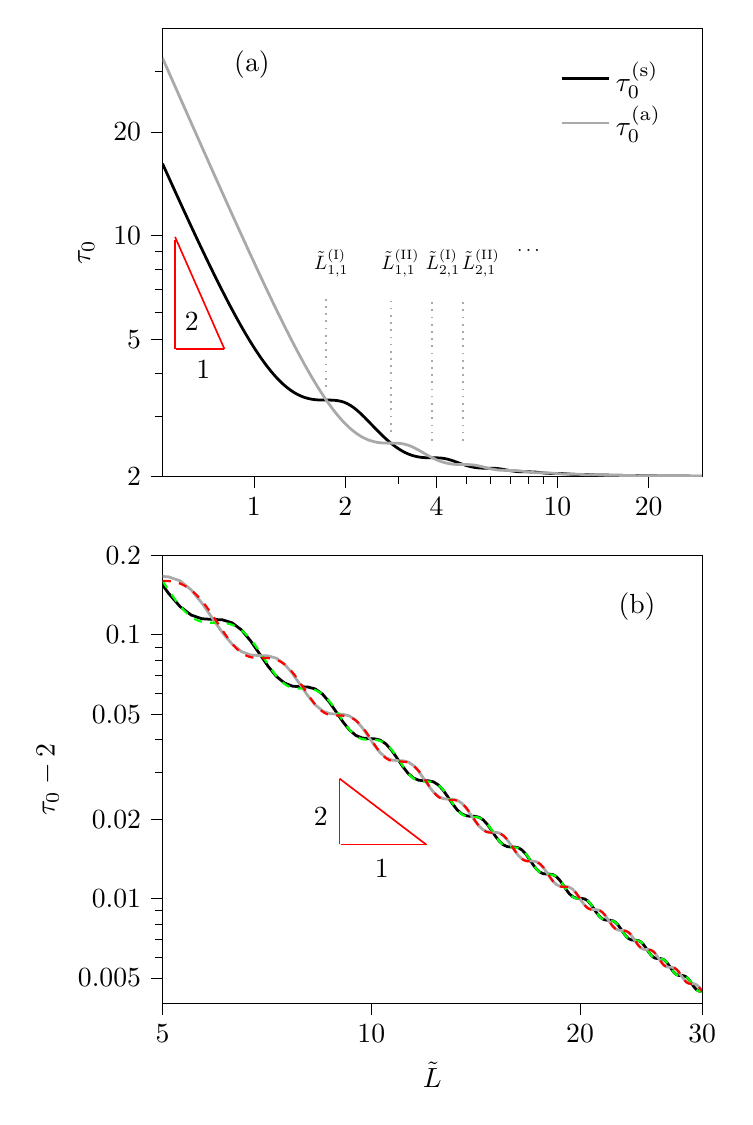
\begin{tikzpicture}

\definecolor{darkgray}{RGB}{169,169,169}
\definecolor{darkgray176}{RGB}{176,176,176}

\begin{groupplot}[group style={group size=1 by 2}]
\nextgroupplot[
log ticks with fixed point, %afegit a ma
ytick={2,5,10,20}, %afegit a ma
minor ytick={3,4,6,7,8,9,30}, %afegit a ma
xtick={1,2,4,10,20}, %afegit a ma
minor xtick={3,5,6,7,8,9}, %afegit a ma
legend cell align={left},
legend style={fill opacity=0.8, draw opacity=1, text opacity=1, at={(0.95,0.95)}, draw=none},
log basis x={10},
log basis y={10},
tick align=outside,
tick pos=left,
x grid style={darkgray176},
xmin=0.5, xmax=30,
xmode=log,
xtick style={color=black},
y grid style={darkgray176},
ylabel={\(\displaystyle \tau_0\)},
ymin=2, ymax=40,
ymode=log,
ytick style={color=black}
]
\addplot [line width=1pt, black]
table {%
0.5 16.1873971654469
0.52 14.9955692399881
0.54 13.9359578067725
0.56 12.990098801246
0.58 12.1426554171925
0.6 11.3808033050015
0.62 10.6937522863086
0.64 10.0723710081298
0.66 9.50888997247584
0.68 8.99666478023081
0.7 8.5299860288148
0.72 8.10392564441343
0.74 7.71421188049086
0.76 7.35712702908208
0.78 7.02942324700963
0.8 6.72825292030247
0.82 6.45111076531796
0.84 6.19578545798727
0.86 5.96031903929238
0.88 5.74297269919318
0.9 5.54219781754253
0.92 5.35661135744574
0.94 5.18497487778882
0.96 5.02617656762402
0.98 4.87921581360383
1 4.7431898986731
1.02 4.61728250035039
1.04 4.50075371369173
1.06 4.39293137017771
1.08 4.29320346143936
1.1 4.20101150761725
1.12 4.11584473555358
1.14 4.03723495299532
1.16 3.96475202236877
1.18 3.89799985213701
1.2 3.83661283580419
1.22 3.78025267871402
1.24 3.72860556125143
1.26 3.68137959417931
1.28 3.63830252785762
1.3 3.59911968219061
1.32 3.56359206848789
1.34 3.53149467813925
1.36 3.50261491620545
1.38 3.47675116081516
1.4 3.45371143172086
1.42 3.43331215358275
1.44 3.41537700159799
1.46 3.3997358190469
1.48 3.38622359826666
1.5 3.37467951856636
1.52 3.36494603675231
1.54 3.3568680283309
1.56 3.35029198019372
1.58 3.34506523876448
1.6 3.34103532128661
1.62 3.33804930222195
1.64 3.3359532916368
1.66 3.33459202791697
1.68 3.33380861300257
1.7 3.33344442421368
1.72 3.33333924205736
1.74 3.33333163727308
1.76 3.33325966156223
1.78 3.33296188341514
1.8 3.33227880145649
1.82 3.33105465109557
1.84 3.32913959480442
1.86 3.32639225195012
1.88 3.32268248241901
1.9 3.31789429320694
1.92 3.31192869502812
1.94 3.30470630493384
1.96 3.29616947940436
1.98 3.28628377701964
2 3.27503859310346
2.02 3.2624468773298
2.04 3.24854392990884
2.06 3.23338535917859
2.08 3.21704435882347
2.1 3.19960851481965
2.12 3.18117637431073
2.14 3.1618540010999
2.16 3.14175171093658
2.18 3.12098113314365
2.2 3.09965269289594
2.22 3.077873558702
2.24 3.05574605784447
2.26 3.03336653137667
2.28 3.01082458008055
2.3 2.98820264230395
2.32 2.96557584174608
2.34 2.94301204578965
2.36 2.92057208083387
2.38 2.89831005861214
2.4 2.87627377548193
2.42 2.85450515436404
2.44 2.83304070592929
2.46 2.81191199157288
2.48 2.79114607563233
2.5 2.77076595824993
2.52 2.75079098336004
2.54 2.73123721862548
2.56 2.7121178058846
2.58 2.69344328192268
2.6 2.6752218702529
2.62 2.65745974517188
2.64 2.64016126971595
2.66 2.62332920934319
2.68 2.60696492324937
2.7 2.59106853522729
2.72 2.57563908592478
2.74 2.56067466826703
2.76 2.54617254769756
2.78 2.53212926876976
2.8 2.51854074949485
2.82 2.50540236472681
2.84 2.49270901974457
2.86 2.48045521507725
2.88 2.46863510351212
2.9 2.45724254012673
2.92 2.44627112609667
2.94 2.43571424694899
2.96 2.42556510585734
2.98 2.41581675250848
3 2.40646210800992
3.02 2.39749398625543
3.04 2.38890511211673
3.06 2.38068813678772
3.08 2.37283565056923
3.1 2.36534019334859
3.12 2.35819426299837
3.14 2.35139032189195
3.16 2.34492080170994
3.18 2.33877810669068
3.2 2.33295461545946
3.22 2.32744268155518
3.24 2.32223463275883
3.26 2.31732276931604
3.28 2.31269936113546
3.3 2.30835664403593
3.32 2.30428681510831
3.34 2.30048202725224
3.36 2.29693438294397
3.38 2.29363592728941
3.4 2.29057864041559
3.42 2.28775442925503
3.44 2.28515511878069
3.46 2.2827724427543
3.48 2.28059803405852
3.5 2.27862341469332
3.52 2.27683998553009
3.54 2.27523901593273
3.56 2.27381163337438
3.58 2.27254881320159
3.6 2.27144136872421
3.62 2.27047994184068
3.64 2.2696549944431
3.66 2.26895680088598
3.68 2.26837544184565
3.7 2.26790079994381
3.72 2.26752255755767
3.74 2.26723019728936
3.76 2.2670130056165
3.78 2.26686008029186
3.8 2.26676034209918
3.82 2.2667025516004
3.84 2.26667533152177
3.86 2.26666719541617
3.88 2.2666665832009
3.9 2.26666190409579
3.92 2.26664158737033
3.94 2.26659414114375
3.96 2.26650821926418
3.98 2.26637269602117
4 2.26617674812126
4.02 2.26590994298664
4.04 2.26556233203532
4.06 2.26512454718659
4.08 2.26458789843406
4.1 2.26394446997055
4.12 2.26318721206893
4.14 2.26231002575388
4.16 2.26130783727222
4.18 2.26017665950526
4.2 2.25891363777606
4.22 2.25751707798195
4.24 2.25598645560758
4.26 2.2543224049088
4.28 2.25252668835411
4.3 2.25060214721103
4.32 2.24855263491284
4.34 2.24638293548235
4.36 2.24409866978402
4.38 2.24170619269595
4.4 2.23921248442968
4.42 2.23662503918596
4.44 2.23395175413835
4.46 2.23120082141602
4.48 2.22838062534809
4.5 2.22549964677324
4.52 2.22256637574402
4.54 2.21958923349715
4.56 2.21657650414071
4.58 2.21353627614284
4.6 2.21047639340351
4.62 2.20740441545301
4.64 2.2043275861464
4.66 2.20125281010682
4.68 2.19818663610416
4.7 2.1951352465315
4.72 2.19210445215
4.74 2.18909969130661
4.76 2.1861260328796
4.78 2.18318818226912
4.8 2.18029048981813
4.82 2.17743696111904
4.84 2.17463126873094
4.86 2.17187676489802
4.88 2.16917649492177
4.9 2.16653321089553
4.92 2.16394938556033
4.94 2.16142722608587
4.96 2.15896868761904
4.98 2.15657548647618
5 2.15424911288377
5.02 2.15199084319659
5.04 2.14980175154224
5.06 2.147682720858
5.08 2.14563445329937
5.1 2.14365748001086
5.12 2.14175217025838
5.14 2.1399187399295
5.16 2.13815725941347
5.18 2.13646766087674
5.2 2.13484974495311
5.22 2.1333031868696
5.24 2.131827542031
5.26 2.13042225108692
5.28 2.12908664450602
5.3 2.12781994668234
5.32 2.1266212795992
5.34 2.12548966607597
5.36 2.12442403262355
5.38 2.12342321193424
5.4 2.1224859450324
5.42 2.12161088311237
5.44 2.12079658909131
5.46 2.1200415389051
5.48 2.11934412257704
5.5 2.11870264509048
5.52 2.1181153270986
5.54 2.11758030550663
5.56 2.11709563396506
5.58 2.1166592833148
5.6 2.11626914202972
5.62 2.1159230167054
5.64 2.11561863264758
5.66 2.11535363461882
5.68 2.11512558780664
5.7 2.11493197908206
5.72 2.1147702186227
5.74 2.11463764197988
5.76 2.11453151267443
5.78 2.11444902540993
5.8 2.11438730999594
5.82 2.11434343607585
5.84 2.11431441875434
5.86 2.1142972252177
5.88 2.11428878243573
5.9 2.11428598602576
5.92 2.11428571034752
5.94 2.11428481988129
5.96 2.11428018192038
5.98 2.11426868058257
6 2.11424723211327
6.02 2.11421280141656
6.04 2.11416241970824
6.06 2.11409320314003
6.08 2.11400237219614
6.1 2.11388727161493
6.12 2.11374539054114
6.14 2.11357438257128
6.16 2.11337208531778
6.18 2.113136539091
6.2 2.11286600428265
6.22 2.11255897703378
6.24 2.112214202786
6.26 2.11183068734652
6.28 2.11140770514672
6.3 2.11094480443817
6.32 2.11044180924731
6.34 2.10989881799695
6.36 2.1093161987953
6.38 2.10869458148667
6.4 2.10803484664758
6.42 2.10733811179369
6.44 2.10660571513187
6.46 2.10583919724653
6.48 2.10504028114617
6.5 2.10421085111581
6.52 2.1033529308232
6.54 2.10246866111246
6.56 2.10156027789147
6.58 2.10063009047997
6.6 2.09968046073861
6.62 2.0987137832465
6.64 2.09773246674086
6.66 2.09673891697788
6.68 2.09573552112251
6.7 2.09472463372725
6.72 2.09370856431782
6.74 2.09268956656764
6.76 2.09166982901247
6.78 2.09065146723346
6.8 2.08963651741847
6.82 2.08862693119917
6.84 2.08762457165363
6.86 2.08663121036043
6.88 2.08564852538979
6.9 2.08467810011975
6.92 2.08372142276967
6.94 2.08277988654942
6.96 2.08185479032943
6.98 2.08094733974443
7 2.08005864865176
7.02 2.07918974087269
7.04 2.07834155215348
7.06 2.0775149322899
7.08 2.07671064736627
7.1 2.07592938206639
7.12 2.07517174202013
7.14 2.07443825615445
7.16 2.07372937902305
7.18 2.07304549309295
7.2 2.07238691097054
7.22 2.07175387755295
7.24 2.07114657209393
7.26 2.07056511017585
7.28 2.07000954558228
7.3 2.06947987206739
7.32 2.06897602502039
7.34 2.0684978830251
7.36 2.068045269316
7.38 2.06761795313356
7.4 2.06721565098299
7.42 2.06683802780162
7.44 2.06648469804133
7.46 2.06615522667345
7.48 2.0658491301246
7.5 2.06556587715331
7.52 2.06530488967781
7.54 2.06506554356717
7.56 2.06484716940859
7.58 2.06464905326516
7.6 2.06447043743968
7.62 2.06431052126128
7.64 2.06416846191315
7.66 2.0640433753209
7.68 2.06393433712261
7.7 2.0638403837428
7.72 2.06376051359411
7.74 2.06369368843145
7.76 2.06363883488448
7.78 2.06359484619516
7.8 2.06356058418743
7.82 2.06353488149637
7.84 2.06351654408356
7.86 2.06350435406449
7.88 2.0634970728722
7.9 2.06349344477845
7.92 2.06349220079073
7.94 2.06349206293846
7.96 2.06349174895635
7.98 2.06348997736599
8 2.06348547294887
8.02 2.06347697259496
8.04 2.0634632315006
8.06 2.06344302967882
8.08 2.06341517873328
8.1 2.06337852883498
8.12 2.06333197582926
8.14 2.06327446838874
8.16 2.06320501511775
8.18 2.06312269150485
8.2 2.06302664661306
8.22 2.06291610939365
8.24 2.06279039450801
8.26 2.06264890754462
8.28 2.0624911495242
8.3 2.06231672059589
8.32 2.0621253228407
8.34 2.06191676211515
8.36 2.06169094888722
8.38 2.06144789803842
8.4 2.06118772762824
8.42 2.06091065664047
8.44 2.06061700175315
8.46 2.06030717319493
8.48 2.05998166976947
8.5 2.0596410731449
8.52 2.05928604151786
8.54 2.05891730277006
8.56 2.05853564723963
8.58 2.05814192023065
8.6 2.05773701438111
8.62 2.05732186200387
8.64 2.05689742750632
8.66 2.05646469998426
8.68 2.0560246860727
8.7 2.0555784031241
8.72 2.05512687277048
8.74 2.05467111491328
8.76 2.05421214217159
8.78 2.05375095480828
8.8 2.05328853614237
8.82 2.05282584844685
8.84 2.05236382932324
8.86 2.05190338853719
8.88 2.05144540529446
8.9 2.05099072593215
8.92 2.0505401619976
8.94 2.05009448868486
8.96 2.04965444359811
8.98 2.04922072581101
9 2.04879399519105
9.02 2.04837487195922
9.04 2.0479639364564
9.06 2.0475617290893
9.08 2.04716875043073
9.1 2.04678546145073
9.12 2.04641228385709
9.14 2.04604960052567
9.16 2.04569775600298
9.18 2.04535705706525
9.2 2.04502777332013
9.22 2.04471013783883
9.24 2.04440434780807
9.26 2.04411056519291
9.28 2.04382891740275
9.3 2.04355949795427
9.32 2.04330236712615
9.34 2.04305755260169
9.36 2.04282505009644
9.38 2.04260482396885
9.4 2.04239680781304
9.42 2.0422009050335
9.44 2.04201698940235
9.46 2.04184490560068
9.48 2.04168446974609
9.5 2.04153546990932
9.52 2.04139766662363
9.54 2.04127079339101
9.56 2.04115455719039
9.58 2.04104863899319
9.6 2.04095269429266
9.62 2.04086635365359
9.64 2.04078922329019
9.66 2.04072088567994
9.68 2.04066090022218
9.7 2.04060880395057
9.72 2.04056411230911
9.74 2.04052632000159
9.76 2.04049490192502
9.78 2.04046931419737
9.8 2.0404489952903
9.82 2.04043336727724
9.84 2.04042183720701
9.86 2.04041379861241
9.88 2.04040863316249
9.9 2.04040571246615
9.92 2.04040440003294
9.94 2.04040405339549
9.96 2.04040402639546
9.98 2.04040367163249
10 2.04040234307249
10.02 2.04039939880854
10.04 2.04039420396355
10.06 2.0403861337203
10.08 2.04037457646003
10.1 2.0403589369866
10.12 2.04033863980881
10.14 2.04031313244968
10.16 2.04028188874712
10.18 2.04024441210757
10.2 2.04020023867119
10.22 2.04014894034506
10.24 2.04009012766023
10.26 2.04002345240803
10.28 2.0399486100127
10.3 2.03986534159939
10.32 2.03977343572052
10.34 2.03967272970808
10.36 2.03956311062558
10.38 2.03944451579972
10.4 2.03931693291978
10.42 2.03918039970043
10.44 2.03903500311193
10.46 2.0388808781898
10.48 2.03871820644361
10.5 2.03854721389205
10.52 2.03836816875732
10.54 2.03818137885735
10.56 2.0379871887386
10.58 2.03778597659468
10.6 2.03757815101798
10.62 2.03736414763166
10.64 2.03714442564844
10.66 2.03691946440108
10.68 2.03668975988617
10.7 2.03645582135981
10.72 2.03621816801938
10.74 2.03597732580122
10.76 2.03573382431942
10.78 2.03548819396626
10.8 2.03524096318993
10.82 2.03499265596125
10.84 2.03474378943646
10.86 2.03449487181971
10.88 2.03424640042555
10.9 2.0339988599386
10.92 2.03375272086533
10.94 2.03350843817075
10.96 2.03326645009117
10.98 2.03302717711321
11 2.03279102110787
11.02 2.03255836460865
11.04 2.03232957022162
11.06 2.03210498015605
11.08 2.03188491586383
11.1 2.03166967777649
11.12 2.03145954512915
11.14 2.03125477586096
11.16 2.03105560658255
11.18 2.03086225260161
11.2 2.03067490799822
11.22 2.03049374574249
11.24 2.03031891784783
11.26 2.03015055555358
11.28 2.02998876953189
11.3 2.02983365011387
11.32 2.02968526753138
11.34 2.02954367217064
11.36 2.02940889483526
11.38 2.02928094701629
11.4 2.02915982116764
11.42 2.02904549098589
11.44 2.02893791169373
11.46 2.028837020327
11.48 2.02874273602562
11.5 2.02865496032922
11.52 2.02857357747862
11.54 2.0284984547249
11.56 2.02842944264794
11.58 2.02836637548694
11.6 2.0283090714857
11.62 2.02825733325564
11.64 2.02821094816023
11.66 2.02816968872445
11.68 2.02813331307334
11.7 2.02810156540404
11.72 2.02807417649571
11.74 2.02805086426208
11.76 2.02803133435144
11.78 2.02801528079881
11.8 2.02800238673517
11.82 2.02799232515838
11.84 2.02798475977036
11.86 2.02797934588435
11.88 2.02797573140634
11.9 2.02797355789326
11.92 2.02797246169059
11.94 2.02797207515055
11.96 2.02797202793126
11.98 2.02797194837601
12 2.02797146497024
12.02 2.02797020787236
12.04 2.02796781051306
12.06 2.02796391125555
12.08 2.02795815510779
12.1 2.02795019547547
12.12 2.02793969594294
12.14 2.0279263320671
12.16 2.027909793168
12.18 2.02788978409793
12.2 2.02786602696988
12.22 2.02783826282502
12.24 2.02780625321849
12.26 2.02776978170246
12.28 2.02772865518596
12.3 2.0276827051515
12.32 2.02763178871012
12.34 2.02757578947822
12.36 2.0275146182617
12.38 2.02744821353588
12.4 2.02737654171264
12.42 2.02729959718953
12.44 2.02721740217927
12.46 2.0271300063215
12.48 2.02703748608243
12.5 2.02693994395122
12.52 2.02683750744536
12.54 2.02673032793997
12.56 2.02661857933852
12.58 2.0265024566043
12.6 2.02638217417361
12.62 2.02625796427245
12.64 2.0261300751589
12.66 2.02599876931333
12.68 2.02586432159812
12.7 2.0257270174073
12.72 2.02558715082571
12.74 2.02544502281504
12.76 2.02530093944283
12.78 2.02515521016833
12.8 2.02500814619693
12.82 2.02486005891305
12.84 2.02471125839926
12.86 2.0245620520473
12.88 2.02441274326503
12.9 2.02426363028157
12.92 2.02411500505136
12.94 2.02396715225642
12.96 2.02382034840512
12.98 2.02367486102474
13 2.02353094794397
13.02 2.02338885666151
13.04 2.02324882379569
13.06 2.0231110746103
13.08 2.02297582261136
13.1 2.02284326920932
13.12 2.0227136034415
13.14 2.02258700174941
13.16 2.02246362780583
13.18 2.02234363238675
13.2 2.0222271532835
13.22 2.02211431525065
13.24 2.02200522998565
13.26 2.02189999613642
13.28 2.02179869933353
13.3 2.02170141224385
13.32 2.021608194643
13.34 2.02151909350419
13.36 2.02143414310146
13.38 2.02135336512549
13.4 2.02127676881087
13.42 2.02120435107342
13.44 2.02113609665711
13.46 2.02107197828998
13.48 2.02101195684884
13.5 2.02095598153304
13.52 2.02090399004751
13.54 2.02085590879579
13.56 2.02081165308391
13.58 2.02077112733626
13.6 2.02073422532476
13.62 2.02070083041283
13.64 2.02067081581605
13.66 2.02064404488129
13.68 2.02062037138639
13.7 2.0205996398627
13.72 2.02058168594279
13.74 2.02056633673552
13.76 2.02055341123127
13.78 2.02054272073946
13.8 2.02053406936091
13.82 2.02052725449734
13.84 2.02052206740017
13.86 2.02051829376049
13.88 2.02051571434205
13.9 2.02051410565836
13.92 2.02051324069495
13.94 2.02051288967714
13.96 2.02051282088309
13.98 2.02051280150121
14 2.02051259853043
14.02 2.02051197972079
14.04 2.02051071455111
14.06 2.02050857523941
14.08 2.02050533778108
14.1 2.0205007830084
14.12 2.02049469766453
14.14 2.02048687548367
14.16 2.02047711826876
14.18 2.02046523695678
14.2 2.0204510526615
14.22 2.02043439768271
14.24 2.02041511647091
14.26 2.0203930665361
14.28 2.02036811928954
14.3 2.02034016080772
14.32 2.02030909250827
14.34 2.02027483172851
14.36 2.02023731219833
14.38 2.02019648440038
14.4 2.02015231581211
14.42 2.02010479102581
14.44 2.02005391174441
14.46 2.01999969665302
14.48 2.01994218116742
14.5 2.01988141706321
14.52 2.01981747199045
14.54 2.01975042888068
14.56 2.01968038525435
14.58 2.01960745243807
14.6 2.01953175470203
14.62 2.0194534283288
14.64 2.01937262062502
14.66 2.01928948888803
14.68 2.01920419933918
14.7 2.01911692603558
14.72 2.01902784977152
14.74 2.01893715698019
14.76 2.01884503864552
14.78 2.01875168923318
14.8 2.01865730564873
14.82 2.01856208622993
14.84 2.01846622977911
14.86 2.01836993464061
14.88 2.01827339782701
14.9 2.0181768141972
14.92 2.01808037568815
14.94 2.0179842706016
14.96 2.01788868294602
14.98 2.01779379183348
15 2.01769977093064
15.02 2.01760678796233
15.04 2.01751500426602
15.06 2.01742457439502
15.08 2.01733564576796
15.1 2.01724835836199
15.12 2.01716284444708
15.14 2.01707922835851
15.16 2.01699762630492
15.18 2.01691814620912
15.2 2.01684088757894
15.22 2.01676594140566
15.24 2.01669339008745
15.26 2.01662330737565
15.28 2.01655575834162
15.3 2.0164907993623
15.32 2.01642847812263
15.34 2.01636883363329
15.36 2.01631189626232
15.38 2.01625768777942
15.4 2.01620622141191
15.42 2.01615750191156
15.44 2.01611152563164
15.46 2.01606828061364
15.48 2.01602774668361
15.5 2.01598989555776
15.52 2.01595469095765
15.54 2.01592208873497
15.56 2.01589203700652
15.58 2.01586447629978
15.6 2.0158393397098
15.62 2.01581655306832
15.64 2.0157960351258
15.66 2.01577769774781
15.68 2.01576144612642
15.7 2.0157471790083
15.72 2.01573478894034
15.74 2.01572416253457
15.76 2.01571518075322
15.78 2.0157077192157
15.8 2.01570164852845
15.82 2.01569683463906
15.84 2.01569313921568
15.86 2.01569042005278
15.88 2.01568853150394
15.9 2.01568732494235
15.92 2.0156866492493
15.94 2.01568635133056
15.96 2.01568627666048
15.98 2.01568626985293
16 2.0156861752579
16.02 2.01568583758215
16.04 2.01568510253175
16.06 2.01568381747376
16.08 2.0156818321139
16.1 2.01567899918634
16.12 2.01567517515137
16.14 2.01567022089607
16.16 2.01566400243267
16.18 2.01565639158883
16.2 2.01564726668376
16.22 2.01563651318377
16.24 2.01562402433066
16.26 2.01560970173634
16.28 2.01559345593697
16.3 2.01557520690043
16.32 2.01555488448069
16.34 2.01553242881371
16.36 2.01550779064958
16.38 2.01548093161658
16.4 2.01545182441358
16.42 2.01542045292801
16.44 2.01538681227775
16.46 2.01535090877614
16.48 2.01531275982055
16.5 2.01527239370568
16.52 2.0152298493642
16.54 2.01518517603784
16.56 2.01513843288323
16.58 2.0150896885175
16.6 2.0150390205092
16.62 2.01498651482087
16.64 2.01493226520961
16.66 2.01487637259291
16.68 2.01481894438634
16.7 2.01476009382033
16.72 2.01469993924296
16.74 2.01463860341519
16.76 2.01457621280504
16.78 2.01451289688654
16.8 2.01444878744885
16.82 2.01438401792037
16.84 2.01431872271232
16.86 2.01425303658527
16.88 2.01418709404197
16.9 2.01412102874883
16.92 2.01405497298819
16.94 2.01398905714277
16.96 2.01392340921322
16.98 2.01385815436932
17 2.01379341453496
17.02 2.01372930800651
17.04 2.01366594910416
17.06 2.01360344785519
17.08 2.01354190970835
17.1 2.01348143527788
17.12 2.01342212011595
17.14 2.01336405451195
17.16 2.01330732331725
17.18 2.01325200579368
17.2 2.01319817548437
17.22 2.01314590010524
17.24 2.01309524145582
17.26 2.01304625534779
17.28 2.0129989915501
17.3 2.01295349374918
17.32 2.01290979952326
17.34 2.01286794032956
17.36 2.01282794150361
17.38 2.01278982226967
17.4 2.01275359576157
17.42 2.01271926905345
17.44 2.01268684319985
17.46 2.01265631328473
17.48 2.01262766847925
17.5 2.01260089210818
17.52 2.01257596172477
17.54 2.0125528491943
17.56 2.01253152078649
17.58 2.01251193727683
17.6 2.01249405405758
17.62 2.01247782125843
17.64 2.01246318387777
17.66 2.01245008192483
17.68 2.01243845057359
17.7 2.01242822032901
17.72 2.01241931720633
17.74 2.01241166292426
17.76 2.0124051751128
17.78 2.01239976753633
17.8 2.01239535033288
17.82 2.01239183027006
17.84 2.01238911101837
17.86 2.01238709344232
17.88 2.01238567590973
17.9 2.01238475461955
17.92 2.01238422394804
17.94 2.01238397681341
17.96 2.01238390505837
17.98 2.01238389985004
18 2.01238385209638
18.02 2.01238365287778
18.04 2.01238319389256
18.06 2.01238236791429
18.08 2.01238106925895
18.1 2.01237919425944
18.12 2.01237664174451
18.14 2.01237331351904
18.16 2.01236911484236
18.18 2.01236395490071
18.2 2.01235774727021
18.22 2.01235041036605
18.24 2.01234186787392
18.26 2.01233204915933
18.28 2.01232088965073
18.3 2.01230833119232
18.32 2.01229432236258
18.34 2.01227881875502
18.36 2.0122617832177
18.38 2.01224318604875
18.4 2.01222300514527
18.42 2.012201226104
18.44 2.01217784227221
18.46 2.01215285474816
18.48 2.01212627233113
18.5 2.01209811142149
18.52 2.01206839587206
18.54 2.01203715679253
18.56 2.01200443230917
18.58 2.01197026728298
18.6 2.01193471298923
18.62 2.01189782676237
18.64 2.01185967161016
18.66 2.01182031580127
18.68 2.01177983243074
18.7 2.01173829896771
18.72 2.01169579678986
18.74 2.0116524107088
18.76 2.01160822849081
18.78 2.0115633403766
18.8 2.01151783860408
18.82 2.01147181693743
18.84 2.01142537020559
18.86 2.01137859385296
18.88 2.0113315835047
18.9 2.01128443454862
18.92 2.01123724173551
18.94 2.01119009879904
18.96 2.01114309809644
18.98 2.01109633027058
19 2.01104988393391
19.02 2.01100384537446
19.04 2.01095829828372
19.06 2.01091332350637
19.08 2.01086899881128
19.1 2.01082539868315
19.12 2.01078259413431
19.14 2.01074065253576
19.16 2.01069963746655
19.18 2.01065960858077
19.2 2.01062062149113
19.22 2.01058272766816
19.24 2.01054597435423
19.26 2.01051040449135
19.28 2.01047605666202
19.3 2.01044296504217
19.32 2.01041115936551
19.34 2.01038066489854
19.36 2.01035150242556
19.38 2.01032368824311
19.4 2.01029723416334
19.42 2.01027214752579
19.44 2.01024843121737
19.46 2.01022608370011
19.48 2.01020509904651
19.5 2.01018546698243
19.52 2.01016717293729
19.54 2.01015019810179
19.56 2.01013451949307
19.58 2.01012011002747
19.6 2.0101069386012
19.62 2.01009497017904
19.64 2.01008416589146
19.66 2.01007448314042
19.68 2.01006587571442
19.7 2.01005829391298
19.72 2.0100516846812
19.74 2.01004599175463
19.76 2.01004115581515
19.78 2.01003711465807
19.8 2.01003380337106
19.82 2.01003115452496
19.84 2.01002909837726
19.86 2.0100275630881
19.88 2.01002647494912
19.9 2.01002575862517
19.92 2.01002533740895
19.94 2.01002513348816
19.96 2.01002506822507
19.98 2.01002506244779
20 2.01002503675271
20.02 2.01002491181709
20.04 2.0100246087208
20.06 2.0100240492759
20.08 2.01002315636252
20.1 2.0100218542693
20.12 2.01002006903653
20.14 2.01001772879974
20.16 2.01001476413159
20.18 2.01001110837934
20.2 2.01000669799558
20.22 2.01000147285921
20.24 2.00999537658414
20.26 2.00998835681264
20.28 2.0099803654908
20.3 2.00997135912316
20.32 2.00996129900398
20.34 2.00995015142273
20.36 2.00993788784142
20.38 2.00992448504197
20.4 2.00990992524172
20.42 2.00989419617592
20.44 2.00987729114605
20.46 2.00985920903353
20.48 2.00983995427846
20.5 2.00981953682375
20.52 2.00979797202518
20.54 2.00977528052845
20.56 2.00975148811466
20.58 2.00972662551578
20.6 2.00970072820249
20.62 2.00967383614635
20.64 2.0096459935592
20.66 2.0096172486122
20.68 2.00958765313766
20.7 2.00955726231637
20.72 2.0095261343535
20.74 2.009494330146
20.76 2.00946191294428
20.78 2.00942894801109
20.8 2.00939550228008
20.82 2.00936164401658
20.84 2.00932744248285
20.86 2.0092929676098
20.88 2.00925828967717
20.9 2.00922347900353
20.92 2.00918860564772
20.94 2.00915373912271
20.96 2.00911894812299
20.98 2.0090843002658
21 2.00904986184736
21.02 2.00901569761388
21.04 2.00898187054769
21.06 2.00894844166864
21.08 2.00891546985048
21.1 2.00888301165207
21.12 2.00885112116309
21.14 2.00881984986386
21.16 2.0087892464987
21.18 2.00875935696247
21.2 2.00873022419965
21.22 2.00870188811533
21.24 2.00867438549772
21.26 2.00864774995136
21.28 2.00862201184063
21.3 2.00859719824305
21.32 2.00857333291162
21.34 2.00855043624596
21.36 2.00852852527168
21.38 2.00850761362761
21.4 2.00848771156041
21.42 2.0084688259265
21.44 2.00845096020072
21.46 2.00843411449176
21.48 2.00841828556409
21.5 2.00840346686624
21.52 2.0083896485654
21.54 2.00837681758837
21.56 2.00836495766876
21.58 2.00835404940067
21.6 2.00834407029878
21.62 2.00833499486516
21.64 2.00832679466293
21.66 2.00831943839687
21.68 2.00831289200144
21.7 2.00830711873622
21.72 2.00830207928926
21.74 2.00829773188843
21.76 2.00829403242112
21.78 2.00829093456259
21.8 2.00828838991311
21.82 2.00828634814415
21.84 2.00828475715379
21.86 2.00828356323147
21.88 2.0082827112321
21.9 2.00828214475957
21.92 2.00828180635942
21.94 2.00828163772076
21.96 2.00828157988672
21.98 2.00828157347343
22 2.00828155889672
22.02 2.00828147660586
22.04 2.00828126732374
22.06 2.00828087229229
22.08 2.00828023352216
22.1 2.00827929404539
22.12 2.00827799816966
22.14 2.00827629173267
22.16 2.00827412235485
22.18 2.00827143968891
22.2 2.00826819566414
22.22 2.00826434472367
22.24 2.00825984405278
22.26 2.00825465379619
22.28 2.00824873726247
22.3 2.00824206111358
22.32 2.00823459553783
22.34 2.00822631440433
22.36 2.00821719539758
22.38 2.00820722013063
22.4 2.00819637423561
22.42 2.00818464743073
22.44 2.00817203356289
22.46 2.00815853062553
22.48 2.00814414075136
22.5 2.00812887018023
22.52 2.0081127292023
22.54 2.00809573207723
22.56 2.00807789693026
22.58 2.00805924562625
22.6 2.00803980362306
22.62 2.00801959980583
22.64 2.00799866630383
22.66 2.00797703829169
22.68 2.00795475377703
22.7 2.0079318533765
22.72 2.0079083800822
22.74 2.00788437902062
22.76 2.00785989720613
22.78 2.00783498329093
22.8 2.00780968731345
22.82 2.00778406044692
22.84 2.00775815474985
22.86 2.00773202291999
22.88 2.00770571805305
22.9 2.00767929340761
22.92 2.00765280217717
22.94 2.00762629727043
22.96 2.00759983110051
22.98 2.0075734553836
23 2.00754722094803
23.02 2.00752117755351
23.04 2.00749537372135
23.06 2.00746985657525
23.08 2.00744467169328
23.1 2.00741986297056
23.12 2.0073954724926
23.14 2.00737154041929
23.16 2.00734810487901
23.18 2.00732520187284
23.2 2.00730286518828
23.22 2.00728112632235
23.24 2.00726001441352
23.26 2.00723955618231
23.28 2.00721977587987
23.3 2.00720069524454
23.32 2.00718233346578
23.34 2.00716470715517
23.36 2.00714783032428
23.38 2.00713171436902
23.4 2.00711636806021
23.42 2.00710179754023
23.44 2.00708800632541
23.46 2.00707499531413
23.48 2.0070627628004
23.5 2.00705130449296
23.52 2.00704061353957
23.54 2.00703068055682
23.56 2.00702149366516
23.58 2.00701303852936
23.6 2.00700529840431
23.62 2.00699825418649
23.64 2.00699188447089
23.66 2.00698616561386
23.68 2.00698107180169
23.7 2.00697657512542
23.72 2.00697264566174
23.74 2.00696925156035
23.76 2.00696635913784
23.78 2.00696393297832
23.8 2.00696193604084
23.82 2.00696032977382
23.84 2.00695907423638
23.86 2.00695812822694
23.88 2.00695744941877
23.9 2.00695699450256
23.92 2.00695671933594
23.94 2.00695657909964
23.96 2.00695652846018
23.98 2.00695652173856
24 2.00695651308468
24.02 2.00695645665685
24.04 2.00695630680581
24.06 2.00695601826253
24.08 2.00695554632886
24.1 2.00695484707031
24.12 2.00695387750971
24.14 2.00695259582077
24.16 2.00695096152025
24.18 2.00694893565755
24.2 2.00694648100033
24.22 2.00694356221476
24.24 2.00694014603909
24.26 2.00693620144893
24.28 2.00693169981303
24.3 2.00692661503811
24.32 2.0069209237013
24.34 2.0069146051691
24.36 2.00690764170166
24.38 2.00690001854128
24.4 2.00689172398427
24.42 2.00688274943548
24.44 2.0068730894449
24.46 2.00686274172585
24.48 2.00685170715471
24.5 2.00683998975212
24.52 2.0068275966458
24.54 2.00681453801547
24.56 2.00680082702037
24.58 2.00678647971014
24.6 2.00677151492001
24.62 2.00675595415133
24.64 2.00673982143859
24.66 2.00672314320432
24.68 2.00670594810307
24.7 2.00668826685615
24.72 2.00667013207828
24.74 2.00665157809801
24.76 2.00663264077302
24.78 2.00661335730201
24.8 2.00659376603453
24.82 2.00657390628
24.84 2.00655381811732
24.86 2.00653354220616
24.88 2.00651311960116
24.9 2.00649259156977
24.92 2.00647199941495
24.94 2.00645138430322
24.96 2.00643078709894
24.98 2.00641024820512
25 2.00638980741158
25.02 2.0063695037505
25.04 2.00634937535978
25.06 2.00632945935434
25.08 2.00630979170553
25.1 2.00629040712862
25.12 2.00627133897838
25.14 2.00625261915262
25.16 2.00623427800366
25.18 2.00621634425744
25.2 2.00619884494021
25.22 2.00618180531245
25.24 2.00616524880991
25.26 2.00614919699143
25.28 2.00613366949334
25.3 2.00611868399021
25.32 2.00610425616161
25.34 2.00609039966478
25.36 2.00607712611293
25.38 2.00606444505886
25.4 2.00605236398395
25.42 2.00604088829209
25.44 2.00603002130856
25.46 2.00601976428376
25.48 2.00601011640152
25.5 2.00600107479213
25.52 2.00599263454981
25.54 2.00598478875482
25.56 2.0059775285
25.58 2.00597084292191
25.6 2.00596471923643
25.62 2.00595914277912
25.64 2.00595409705012
25.66 2.00594956376387
25.68 2.00594552290371
25.7 2.00594195278136
25.72 2.0059388301015
25.74 2.00593613003148
25.76 2.00593382627628
25.78 2.00593189115879
25.8 2.00593029570556
25.82 2.00592900973793
25.84 2.00592800196873
25.86 2.00592724010446
25.88 2.00592669095287
25.9 2.00592632053608
25.92 2.00592609420881
25.94 2.00592597678184
25.96 2.00592593265022
25.98 2.00592592592626
26 2.00592592057637
26.02 2.00592588056216
26.04 2.00592576998451
26.06 2.00592555323049
26.08 2.00592519512235
26.1 2.0059246610679
26.12 2.00592391721147
26.14 2.0059229305846
26.16 2.0059216692556
26.18 2.00592010247698
26.2 2.00591820082972
26.22 2.00591593636345
26.24 2.00591328273139
26.26 2.00591021531898
26.28 2.0059067113653
26.3 2.00590275007605
26.32 2.00589831272724
26.34 2.00589338275865
26.36 2.00588794585605
26.38 2.00588199002167
26.4 2.00587550563195
26.42 2.00586848548227
26.44 2.00586092481794
26.46 2.00585282135145
26.48 2.00584417526555
26.5 2.00583498920221
26.52 2.00582526823766
26.54 2.00581501984361
26.56 2.00580425383518
26.58 2.00579298230593
26.6 2.00578121955073
26.62 2.00576898197719
26.64 2.00575628800643
26.66 2.00574315796426
26.68 2.00572961396361
26.7 2.00571567977939
26.72 2.00570138071674
26.74 2.00568674347386
26.76 2.00567179600054
26.78 2.00565656735333
26.8 2.00564108754864
26.82 2.00562538741462
26.84 2.00560949844283
26.86 2.00559345264075
26.88 2.00557728238583
26.9 2.0055610202819
26.92 2.00554469901873
26.94 2.00552835123547
26.96 2.00551200938794
26.98 2.00549570562123
27 2.00547947164714
27.02 2.00546333862726
27.04 2.0054473370617
27.06 2.005431496684
27.08 2.00541584636175
27.1 2.00540041400387
27.12 2.0053852264737
27.14 2.00537030950848
27.16 2.00535568764489
27.18 2.00534138415067
27.2 2.00532742096218
27.22 2.00531381862778
27.24 2.00530059625689
27.26 2.00528777147445
27.28 2.00527536038092
27.3 2.00526337751724
27.32 2.00525183583494
27.34 2.00524074667102
27.36 2.00523011972753
27.38 2.00521996305569
27.4 2.0052102830444
27.42 2.00520108441302
27.44 2.0051923702083
27.46 2.00518414180544
27.48 2.00517639891302
27.5 2.00516913958201
27.52 2.00516236021854
27.54 2.00515605560056
27.56 2.00515021889841
27.58 2.00514484169909
27.6 2.00513991403455
27.62 2.00513542441376
27.64 2.00513135985871
27.66 2.00512770594448
27.68 2.00512444684323
27.7 2.00512156537233
27.72 2.00511904304668
27.74 2.00511686013517
27.76 2.00511499572147
27.78 2.00511342776914
27.8 2.00511213319105
27.82 2.00511108792321
27.84 2.00511026700307
27.86 2.00510964465194
27.88 2.00510919436202
27.9 2.00510888898753
27.92 2.00510870083978
27.94 2.00510860178655
27.96 2.00510856335513
27.98 2.00510855683856
28 2.00510855340553
28.02 2.00510852421302
28.04 2.00510844052123
28.06 2.00510827381083
28.08 2.00510799590153
28.1 2.00510757907172
28.12 2.00510699617839
28.14 2.00510622077678
28.16 2.00510522723906
28.18 2.00510399087119
28.2 2.00510248802737
28.22 2.00510069622105
28.24 2.005098594232
28.26 2.00509616220835
28.28 2.00509338176295
28.3 2.00509023606326
28.32 2.00508670991394
28.34 2.00508278983153
28.36 2.00507846411047
28.38 2.00507372287996
28.4 2.00506855815097
28.42 2.00506296385319
28.44 2.00505693586139
28.46 2.00505047201099
28.48 2.00504357210274
28.5 2.00503623789641
28.52 2.00502847309353
28.54 2.00502028330948
28.56 2.005011676035
28.58 2.00500266058768
28.6 2.00499324805375
28.62 2.00498345122085
28.64 2.00497328450227
28.66 2.00496276385339
28.68 2.00495190668118
28.7 2.00494073174729
28.72 2.00492925906585
28.74 2.00491750979653
28.76 2.00490550613394
28.78 2.00489327119398
28.8 2.0048808288982
28.82 2.00486820385675
28.84 2.00485542125086
28.86 2.00484250671544
28.88 2.00482948622258
28.9 2.00481638596657
28.92 2.0048032322509
28.94 2.00479005137812
28.96 2.00477686954227
28.98 2.00476371272536
29 2.00475060659725
29.02 2.00473757641985
29.04 2.00472464695559
29.06 2.00471184238045
29.08 2.00469918620181
29.1 2.00468670118062
29.12 2.00467440925913
29.14 2.00466233149294
29.16 2.00465048798804
29.18 2.0046388978428
29.2 2.00462757909458
29.22 2.00461654867109
29.24 2.00460582234636
29.26 2.00459541470119
29.28 2.00458533908799
29.3 2.00457560759987
29.32 2.00456623104393
29.34 2.00455721891853
29.36 2.00454857939455
29.38 2.00454031930039
29.4 2.0045324441108
29.42 2.0045249579392
29.44 2.00451786353368
29.46 2.00451116227634
29.48 2.00450485418617
29.5 2.00449893792519
29.52 2.00449341080797
29.54 2.00448826881444
29.56 2.00448350660597
29.58 2.00447911754475
29.6 2.00447509371645
29.62 2.00447142595617
29.64 2.00446810387772
29.66 2.00446511590631
29.68 2.00446244931451
29.7 2.00446009026176
29.72 2.00445802383724
29.74 2.00445623410632
29.76 2.00445470416048
29.78 2.00445341617076
29.8 2.0044523514449
29.82 2.00445149048784
29.84 2.0044508130661
29.86 2.00445029827514
29.88 2.00444992461084
29.9 2.00444967004388
29.92 2.00444951209762
29.94 2.00444942792903
29.96 2.00444939441262
29.98 2.00444938822715
30 2.00444938594483
};
\addlegendentry{$\tau_0^{(\text{s})}$}
\addplot [line width=1pt, darkgray]
table {%
0.5 32.7828919351573
0.52 30.3176218724273
0.54 28.1217807262207
0.56 26.157597592197
0.58 24.3936993825357
0.6 22.8038531154049
0.62 21.3659874836861
0.64 20.0614250131859
0.66 18.8742745586187
0.68 17.7909469841802
0.7 16.7997662874843
0.72 15.890655261034
0.74 15.0548797994059
0.76 14.2848396729223
0.78 13.5738963619234
0.8 12.9162306347444
0.82 12.3067241384423
0.84 11.7408604842961
0.86 11.2146422444013
0.88 10.7245210001273
0.9 10.2673381485147
0.92 9.84027461648464
0.94 9.440807983139
0.96 9.06667578862161
0.98 8.71584403002105
1 8.38648002286545
1.02 8.0769289502634
1.04 7.78569353792596
1.06 7.51141638777685
1.08 7.25286458000155
1.1 7.00891621663488
1.12 6.7785486318439
1.14 6.56082803706986
1.16 6.35490040485055
1.18 6.15998342481031
1.2 5.97535939006908
1.22 5.80036889306039
1.24 5.63440522716911
1.26 5.47690940527796
1.28 5.32736571871509
1.3 5.18529777060464
1.32 5.0502649265521
1.34 4.92185913320324
1.36 4.79970206171225
1.38 4.68344253871684
1.4 4.57275423219106
1.42 4.46733356365277
1.44 4.36689782174188
1.46 4.27118345524344
1.48 4.17994452627742
1.5 4.09295130667355
1.52 4.00998900254642
1.54 3.93085659382474
1.56 3.85536577700625
1.58 3.78334000073589
1.6 3.71461358496685
1.62 3.64903091548267
1.64 3.58644570645423
1.66 3.52672032449344
1.68 3.46972516835998
1.7 3.41533809909102
1.72 3.36344391586582
1.74 3.31393387339747
1.76 3.26670523706961
1.78 3.22166087241408
1.8 3.17870886586148
1.82 3.13776217399556
1.84 3.0987382988092
1.86 3.06155898669748
1.88 3.02614994913545
1.9 2.99244060317878
1.92 2.96036383009478
1.94 2.9298557505839
1.96 2.90085551518827
1.98 2.8733051086062
2 2.84714916674165
2.02 2.82233480541631
2.04 2.7988114597609
2.06 2.77653073338216
2.08 2.7554462564738
2.1 2.7355135521047
2.12 2.71668990997589
2.14 2.69893426699067
2.16 2.68220709402981
2.18 2.66647028836723
2.2 2.6516870712006
2.22 2.63782188980733
2.24 2.6248403238696
2.26 2.61270899554247
2.28 2.60139548286827
2.3 2.59086823616799
2.32 2.58109649706714
2.34 2.57205021984068
2.36 2.5636999947893
2.38 2.55601697338814
2.4 2.54897279498128
2.42 2.54253951483014
2.44 2.53668953336431
2.46 2.53139552652965
2.48 2.5266303771826
2.5 2.52236710754396
2.52 2.51857881280088
2.54 2.51523859603567
2.56 2.51231950476638
2.58 2.50979446950901
2.6 2.50763624491763
2.62 2.50581735422854
2.64 2.50431003792933
2.66 2.50308620779414
2.68 2.50211740767187
2.7 2.50137478268093
2.72 2.50082905874767
2.74 2.50045053471385
2.76 2.50020908951885
2.78 2.50007420721139
2.8 2.50001502273648
2.82 2.50000039153947
2.84 2.4999989859877
2.86 2.4999794213812
2.88 2.4999104138558
2.9 2.49976097172364
2.92 2.499500620707
2.94 2.49909966207981
2.96 2.49852946094661
2.98 2.49776275981058
3 2.49677401031557
3.02 2.49553971374712
3.04 2.49403875875811
3.06 2.49225274308938
3.08 2.49016626504527
3.1 2.4877671703852
3.12 2.48504674126734
3.14 2.48199981597932
3.16 2.47862483132981
3.18 2.4749237835282
3.2 2.47090210780203
3.22 2.46656848147279
3.24 2.46193455929408
3.26 2.45701465317126
3.28 2.45182537064914
3.3 2.44638522764175
3.32 2.44071425079599
3.34 2.43483358377206
3.36 2.42876510982215
3.38 2.42253110063517
3.4 2.41615389877337
3.42 2.40965563840537
3.44 2.40305800663499
3.46 2.39638204566558
3.48 2.38964799439344
3.5 2.38287516680558
3.52 2.37608186374232
3.54 2.36928531412264
3.56 2.36250164155772
3.58 2.35574585232753
3.6 2.34903184090515
3.62 2.34237240952746
3.64 2.33577929868445
3.66 2.32926322579702
3.68 2.32283392974876
3.7 2.31650021931407
3.72 2.31027002387035
3.74 2.30415044509185
3.76 2.29814780859287
3.78 2.29226771472086
3.8 2.28651508789515
3.82 2.28089422405085
3.84 2.27540883588011
3.86 2.27006209567106
3.88 2.26485667563023
3.9 2.25979478564147
3.92 2.25487820846565
3.94 2.25010833242457
3.96 2.2454861816404
3.98 2.24101244392242
4 2.23668749640584
4.02 2.23251142905567
4.04 2.22848406615253
4.06 2.22460498587848
4.08 2.22087353811918
4.1 2.21728886059576
4.12 2.21384989343564
4.14 2.21055539228622
4.16 2.20740394006993
4.18 2.20439395747339
4.2 2.20152371225758
4.22 2.19879132747024
4.24 2.19619478863626
4.26 2.19373194999667
4.28 2.19140053986225
4.3 2.18919816514321
4.32 2.1871223151129
4.34 2.18517036446022
4.36 2.18333957568255
4.38 2.18162710086938
4.4 2.18002998292519
4.42 2.17854515627963
4.44 2.17716944713327
4.46 2.17589957328794
4.48 2.17473214361293
4.5 2.1736636572006
4.52 2.1726905022692
4.54 2.17180895487521
4.56 2.17101517750368
4.58 2.17030521761208
4.6 2.1696750062115
4.62 2.16912035657869
4.64 2.16863696320288
4.66 2.16822040108366
4.68 2.16786612550851
4.7 2.16756947245268
4.72 2.16732565975804
4.74 2.16712978926186
4.76 2.16697685006039
4.78 2.16686172310459
4.8 2.16677918733614
4.82 2.16672392757931
4.84 2.16669054440755
4.86 2.16667356620074
4.88 2.16666746359941
4.9 2.16666666654276
4.92 2.16666558404777
4.94 2.16665862684447
4.96 2.16664023292646
4.98 2.16660489600615
5 2.16654719677875
5.02 2.16646183680115
5.04 2.16634367468088
5.06 2.16618776415133
5.08 2.16598939348619
5.1 2.16574412558425
5.12 2.16544783794354
5.14 2.16509676164795
5.16 2.16468751841927
5.18 2.16421715475088
5.2 2.16368317214175
5.22 2.16308355249725
5.24 2.16241677785748
5.26 2.16168184375268
5.28 2.16087826566535
5.3 2.16000607828943
5.32 2.15906582750922
5.34 2.15805855525967
5.36 2.15698577766238
5.38 2.1558494570435
5.4 2.15465196862002
5.42 2.15339606277939
5.44 2.1520848239688
5.46 2.15072162725318
5.48 2.14931009359552
5.5 2.14785404486547
5.52 2.14635745949801
5.54 2.14482442961335
5.56 2.14325912027952
5.58 2.14166573146134
5.6 2.14004846305914
5.62 2.13841148330746
5.64 2.13675890068029
5.66 2.13509473934141
5.68 2.13342291808606
5.7 2.13174723264588
5.72 2.13007134117158
5.74 2.12839875266639
5.76 2.12673281811623
5.78 2.12507672404791
5.8 2.12343348824221
5.82 2.12180595733268
5.84 2.12019680603093
5.86 2.11860853773406
5.88 2.11704348628768
5.9 2.11550381869749
5.92 2.11399153860285
5.94 2.11250849034627
5.96 2.11105636349259
5.98 2.10963669767053
6 2.10825088762681
6.02 2.1069001883994
6.04 2.10558572053099
6.06 2.10430847525693
6.08 2.10306931961345
6.1 2.10186900142253
6.12 2.10070815411816
6.14 2.09958730138708
6.16 2.09850686160309
6.18 2.09746715204023
6.2 2.0964683928546
6.22 2.09551071082865
6.24 2.09459414287549
6.26 2.09371863930329
6.28 2.09288406684251
6.3 2.09209021144063
6.32 2.09133678083088
6.34 2.09062340688291
6.36 2.08994964774467
6.38 2.08931498978611
6.4 2.08871884935619
6.42 2.08816057436604
6.44 2.08763944571196
6.46 2.08715467855329
6.48 2.08670542346125
6.5 2.08629076745606
6.52 2.08590973495133
6.54 2.0855612886258
6.56 2.08524433024471
6.58 2.08495770145441
6.6 2.0847001845762
6.62 2.08447050342735
6.64 2.08426732419945
6.66 2.08408925642701
6.68 2.08393485408121
6.7 2.08380261682669
6.72 2.08369099148142
6.74 2.08359837372225
6.76 2.08352311008074
6.78 2.08346350027579
6.8 2.08341779993077
6.82 2.08338422372344
6.84 2.08336094901684
6.86 2.0833461200177
6.88 2.08333785250644
6.9 2.08333423917865
6.92 2.08333335563161
6.94 2.08333326702174
6.96 2.08333203540849
6.98 2.08332772778765
7 2.08331842480254
7.02 2.08330223010394
7.04 2.08327728031102
7.06 2.08324175550421
7.08 2.08319389015892
7.1 2.08313198440637
7.12 2.08305441548518
7.14 2.08295964922631
7.16 2.0828462513948
7.18 2.08271289869673
7.2 2.08255838924866
7.22 2.08238165230184
7.24 2.08218175701521
7.26 2.08195792007919
7.28 2.08170951200887
7.3 2.08143606194822
7.32 2.081137260857
7.34 2.08081296298776
7.36 2.08046318560085
7.38 2.08008810690766
7.4 2.07968806227653
7.42 2.07926353877804
7.44 2.07881516818622
7.46 2.0783437185868
7.48 2.07785008477295
7.5 2.07733527762998
7.52 2.07680041272532
7.54 2.07624669832572
7.56 2.07567542306291
7.58 2.07508794346069
7.6 2.07448567152274
7.62 2.07387006256182
7.64 2.07324260342891
7.66 2.07260480127679
7.68 2.071958172967
7.7 2.07130423520414
7.72 2.0706444954569
7.74 2.06998044370277
7.76 2.06931354501276
7.78 2.06864523297458
7.8 2.06797690393742
7.82 2.06730991204904
7.84 2.06664556504588
7.86 2.06598512074974
7.88 2.06532978421911
7.9 2.06468070550046
7.92 2.06403897792309
7.94 2.06340563688121
7.96 2.06278165904815
7.98 2.06216796196951
8 2.06156540398468
8.02 2.06097478442976
8.04 2.0603968440777
8.06 2.0598322657759
8.08 2.05928167524457
8.1 2.05874564200319
8.12 2.05822468039576
8.14 2.05771925068914
8.16 2.05722976022167
8.18 2.05675656458253
8.2 2.05629996880507
8.22 2.05586022855954
8.24 2.05543755133355
8.26 2.05503209759015
8.28 2.05464398189578
8.3 2.05427327401186
8.32 2.05391999994541
8.34 2.0535841429557
8.36 2.05326564451492
8.38 2.05296440522247
8.4 2.05268028567332
8.42 2.05241310728192
8.44 2.0521626530644
8.46 2.05192866838238
8.48 2.05171086165292
8.5 2.05150890502986
8.52 2.05132243506267
8.54 2.05115105333994
8.56 2.05099432712537
8.58 2.05085178999507
8.6 2.05072294248584
8.62 2.05060725276501
8.64 2.05050415733331
8.66 2.0504130617731
8.68 2.05033334155512
8.7 2.05026434291782
8.72 2.05020538383407
8.74 2.05015575508057
8.76 2.05011472142602
8.78 2.05008152295433
8.8 2.05005537653952
8.82 2.05003547748859
8.84 2.05002100136848
8.86 2.05001110603243
8.88 2.05000493385987
8.9 2.05000161422213
8.92 2.05000026618448
8.94 2.05000000145165
8.96 2.04999992756113
8.98 2.04999915132408
9 2.04999678250915
9.02 2.04999193775924
9.04 2.04998374472516
9.06 2.04997134639388
9.08 2.04995390558237
9.1 2.04993060956094
9.12 2.04990067476324
9.14 2.04986335153333
9.16 2.04981792885408
9.18 2.04976373899584
9.2 2.04970016202
9.22 2.04962663006934
9.24 2.04954263137559
9.26 2.04944771391535
9.28 2.04934148864815
9.3 2.04922363227481
9.32 2.04909388946125
9.34 2.04895207448114
9.36 2.04879807224137
9.38 2.04863183866557
9.4 2.04845340042389
9.42 2.04826285401031
9.44 2.04806036418182
9.46 2.04784616178682
9.48 2.04762054102204
9.5 2.0473838561675
9.52 2.04713651785856
9.54 2.0468789889605
9.56 2.04661178011645
9.58 2.04633544504209
9.6 2.04605057564112
9.62 2.04575779701435
9.64 2.04545776243224
9.66 2.04515114833578
9.68 2.04483864942524
9.7 2.0445209738892
9.72 2.0441988388192
9.74 2.04387296584767
9.76 2.04354407703906
9.78 2.04321289105678
9.8 2.04288011962147
9.82 2.04254646426956
9.84 2.04221261341539
9.86 2.04187923971481
9.88 2.04154699772406
9.9 2.04121652184385
9.92 2.04088842453574
9.94 2.04056329479582
9.96 2.04024169686885
9.98 2.03992416918498
10 2.03961122350093
10.02 2.03930334422683
10.04 2.03900098792055
10.06 2.03870458293158
10.08 2.03841452917734
10.1 2.0381311980356
10.12 2.03785493233768
10.14 2.03758604644826
10.16 2.0373248264186
10.18 2.03707153020131
10.2 2.03682638791574
10.22 2.03658960215435
10.24 2.0363613483215
10.26 2.03614177499696
10.28 2.03593100431776
10.3 2.03572913237271
10.32 2.03553622960487
10.34 2.03535234121822
10.36 2.03517748758547
10.38 2.03501166465475
10.4 2.03485484435356
10.42 2.0347069749893
10.44 2.03456798164592
10.46 2.03443776657725
10.48 2.03431620959793
10.5 2.03420316847345
10.52 2.03409847931149
10.54 2.034001956957
10.56 2.03391339539435
10.58 2.03383256816002
10.6 2.03375922877004
10.62 2.03369311116663
10.64 2.03363393018928
10.66 2.03358138207541
10.68 2.03353514499677
10.7 2.03349487963748
10.72 2.03346022982046
10.74 2.03343082318883
10.76 2.03340627194928
10.78 2.03338617368447
10.8 2.03337011224137
10.82 2.03335765870255
10.84 2.03334837244693
10.86 2.03334180230617
10.88 2.03333748782231
10.9 2.03333496061137
10.92 2.03333374583655
10.94 2.03333336379353
10.96 2.03333333160879
10.98 2.03333316505008
11 2.03333238044619
11.02 2.0333304967111
11.04 2.03332703746483
11.06 2.033321533241
11.08 2.03331352376835
11.1 2.03330256031048
11.12 2.03328820804546
11.14 2.03327004846435
11.16 2.03324768176481
11.18 2.03322072921417
11.2 2.03318883545427
11.22 2.03315167071895
11.24 2.03310893293458
11.26 2.03306034967348
11.28 2.03300567993123
11.3 2.03294471569959
11.32 2.03287728330946
11.34 2.03280324452083
11.36 2.03272249734027
11.38 2.03263497655103
11.4 2.03254065394497
11.42 2.03243953825116
11.44 2.0323316747608
11.46 2.03221714465379
11.48 2.03209606403722
11.5 2.03196858271102
11.52 2.03183488268052
11.54 2.03169517643941
11.56 2.03154970504999
11.58 2.0313987360497
11.6 2.03124256121503
11.62 2.03108149421432
11.64 2.0309158681813
11.66 2.03074603324057
11.68 2.0305723540147
11.7 2.03039520714112
11.72 2.03021497882429
11.74 2.03003206244639
11.76 2.02984685625644
11.78 2.02965976115518
11.8 2.02947117858964
11.82 2.02928150856848
11.84 2.02909114780634
11.86 2.02890048800254
11.88 2.02870991425727
11.9 2.02851980362581
11.92 2.02833052380973
11.94 2.02814243198216
11.96 2.02795587374267
11.98 2.02777118219647
12 2.02758867715158
12.02 2.02740866442693
12.04 2.02723143526392
12.06 2.02705726583391
12.08 2.02688641683365
12.1 2.02671913316104
12.12 2.02655564366363
12.14 2.0263961609524
12.16 2.02624088127389
12.18 2.02608998443414
12.2 2.02594363376801
12.22 2.02580197614836
12.24 2.02566514202968
12.26 2.02553324552147
12.28 2.02540638448701
12.3 2.02528464066374
12.32 2.02516807980195
12.34 2.02505675181889
12.36 2.02495069096583
12.38 2.02484991600619
12.4 2.02475443040321
12.42 2.02466422251587
12.44 2.02457926580249
12.46 2.02449951903155
12.48 2.02442492649975
12.5 2.02435541825767
12.52 2.02429091034374
12.54 2.0242313050274
12.56 2.02417649106306
12.58 2.02412634395614
12.6 2.02408072624337
12.62 2.02403948778941
12.64 2.02400246610223
12.66 2.02396948666992
12.68 2.02394036332181
12.7 2.02391489861703
12.72 2.02389288426349
12.74 2.0238741015709
12.76 2.02385832194097
12.78 2.0238453073983
12.8 2.02383481116538
12.82 2.02382657828479
12.84 2.02382034629184
12.86 2.02381584594034
12.88 2.02381280198407
12.9 2.02381093401574
12.92 2.02380995736518
12.94 2.0238095840572
12.96 2.02380952382929
12.98 2.02380948520824
13 2.02380917664367
13.02 2.0238083076955
13.04 2.02380659027113
13.06 2.02380373990688
13.08 2.02379947708684
13.1 2.02379352859099
13.12 2.02378562886321
13.14 2.02377552138832
13.16 2.02376296006631
13.18 2.02374771057061
13.2 2.0237295516767
13.22 2.02370827654621
13.24 2.02368369395168
13.26 2.02365562942679
13.28 2.02362392632704
13.3 2.02358844678641
13.32 2.02354907255656
13.34 2.02350570571606
13.36 2.02345826923889
13.38 2.02340670741328
13.4 2.02335098610398
13.42 2.02329109285338
13.44 2.02322703681942
13.46 2.02315884855075
13.48 2.023086579602
13.5 2.02301030199474
13.52 2.02293010753167
13.54 2.02284610697422
13.56 2.02275842909499
13.58 2.02266721961856
13.6 2.0225726400651
13.62 2.02247486651222
13.64 2.02237408829093
13.66 2.02227050663179
13.68 2.02216433327722
13.7 2.02205578907516
13.72 2.02194510256897
13.74 2.02183250859702
13.76 2.02171824691458
13.78 2.02160256084913
13.8 2.02148569599885
13.82 2.02136789898271
13.84 2.02124941624895
13.86 2.02113049294748
13.88 2.02101137187022
13.9 2.02089229246231
13.92 2.02077348990566
13.94 2.02065519427558
13.96 2.02053762976986
13.98 2.02042101400937
14 2.02030555740804
14.02 2.02019146260975
14.04 2.02007892398938
14.06 2.01996812721449
14.08 2.01985924886415
14.1 2.01975245610129
14.12 2.01964790639465
14.14 2.01954574728659
14.16 2.01944611620302
14.18 2.01934914030173
14.2 2.01925493635559
14.22 2.01916361066734
14.24 2.01907525901278
14.26 2.01898996660936
14.28 2.01890780810757
14.3 2.01882884760267
14.32 2.01875313866442
14.34 2.01868072438311
14.36 2.01861163742989
14.38 2.01854590013027
14.4 2.0184835245493
14.42 2.01842451258777
14.44 2.01836885608846
14.46 2.01831653695222
14.48 2.01826752726336
14.5 2.01822178942465
14.52 2.01817927630178
14.54 2.01813993137793
14.56 2.01810368891893
14.58 2.01807047414979
14.6 2.01804020344355
14.62 2.01801278452359
14.64 2.0179881166807
14.66 2.01796609100613
14.68 2.01794659064245
14.7 2.0179294910536
14.72 2.01791466031589
14.74 2.0179019594318
14.76 2.01789124266829
14.78 2.01788235792143
14.8 2.01787514710908
14.82 2.01786944659332
14.84 2.01786508763414
14.86 2.01786189687579
14.88 2.01785969686688
14.9 2.0178583066152
14.92 2.01785754217769
14.94 2.01785721728582
14.96 2.01785714400594
14.98 2.0178571334339
15 2.01785699642252
15.02 2.01785654433991
15.04 2.01785558985598
15.06 2.01785394775382
15.08 2.01785143576191
15.1 2.01784787540234
15.12 2.01784309284958
15.14 2.01783691979362
15.16 2.01782919430066
15.18 2.01781976166399
15.2 2.01780847523714
15.22 2.01779519724113
15.24 2.01777979953728
15.26 2.01776216435707
15.28 2.01774218498053
15.3 2.01771976635488
15.32 2.0176948256456
15.34 2.01766729271283
15.36 2.01763711050642
15.38 2.01760423537432
15.4 2.01756863727979
15.42 2.01753029992419
15.44 2.01748922077343
15.46 2.01744541098749
15.48 2.01739889525374
15.5 2.01734971152619
15.52 2.01729791067418
15.54 2.01724355604506
15.56 2.01718672294674
15.58 2.01712749805686
15.6 2.01706597876604
15.62 2.01700227246366
15.64 2.01693649577464
15.66 2.01686877375625
15.68 2.01679923906415
15.7 2.01672803109632
15.72 2.01665529512403
15.74 2.01658118141782
15.76 2.01650584437657
15.78 2.01642944166694
15.8 2.0163521333795
15.82 2.01627408120776
15.84 2.01619544765479
15.86 2.01611639527204
15.88 2.01603708593364
15.9 2.01595768014915
15.92 2.01587833641663
15.94 2.01579921061752
15.96 2.01572045545412
15.98 2.01564221992981
16 2.01556464887172
16.02 2.01548788249528
16.04 2.01541205600942
16.06 2.01533729926117
16.08 2.01526373641797
16.1 2.01519148568598
16.12 2.01512065906239
16.14 2.01505136211977
16.16 2.01498369382044
16.18 2.01491774635863
16.2 2.01485360502866
16.22 2.01479134811693
16.24 2.01473104681595
16.26 2.01467276515853
16.28 2.01461655997045
16.3 2.01456248084007
16.32 2.01451057010338
16.34 2.01446086284327
16.36 2.01441338690173
16.38 2.01436816290414
16.4 2.01432520429465
16.42 2.01428451738201
16.44 2.01424610139528
16.46 2.01420994854901
16.48 2.01417604411761
16.5 2.01414436651873
16.52 2.01411488740582
16.54 2.0140875717698
16.56 2.01406237805026
16.58 2.01403925825649
16.6 2.01401815809889
16.62 2.01399901713133
16.64 2.01398176890519
16.66 2.0139663411358
16.68 2.01395265588218
16.7 2.01394062974106
16.72 2.01393017405598
16.74 2.01392119514263
16.76 2.01391359453132
16.78 2.01390726922758
16.8 2.01390211199195
16.82 2.0138980116397
16.84 2.01389485336137
16.86 2.01389251906491
16.88 2.01389088773976
16.9 2.01388983584342
16.92 2.01388923771064
16.94 2.01388896598501
16.96 2.01388889207281
16.98 2.01388888661812
17 2.01388881999856
17.02 2.01388856283987
17.04 2.01388798654782
17.06 2.01388696385513
17.08 2.01388536938078
17.1 2.01388308019874
17.12 2.0138799764125
17.14 2.01387594173178
17.16 2.01387086404693
17.18 2.01386463599669
17.2 2.01385715552429
17.22 2.01384832641697
17.24 2.01383805882362
17.26 2.01382626974538
17.28 2.01381288349392
17.3 2.01379783211236
17.32 2.01378105575392
17.34 2.0137625030139
17.36 2.01374213121077
17.38 2.01371990661291
17.4 2.01369580460808
17.42 2.01366980981324
17.44 2.01364191612335
17.46 2.01361212669834
17.48 2.01358045388832
17.5 2.01354691909789
17.52 2.01351155259127
17.54 2.0134743932406
17.56 2.01343548822057
17.58 2.01339489265312
17.6 2.0133526692064
17.62 2.01330888765296
17.64 2.013263624392
17.66 2.0132169619412
17.68 2.01316898840364
17.7 2.01311979691519
17.72 2.01306948507799
17.74 2.01301815438536
17.76 2.01296590964313
17.78 2.01291285839234
17.8 2.01285911033774
17.82 2.01280477678613
17.84 2.01274997009825
17.86 2.01269480315734
17.88 2.01263938885728
17.9 2.0125838396124
17.92 2.01252826689096
17.94 2.01247278077365
17.96 2.01241748953818
17.98 2.01236249927061
18 2.01230791350364
18.02 2.01225383288206
18.04 2.01220035485479
18.06 2.01214757339341
18.08 2.01209557873619
18.1 2.01204445715685
18.12 2.01199429075714
18.14 2.01194515728212
18.16 2.01189712995701
18.18 2.01185027734441
18.2 2.01180466322076
18.22 2.0117603464708
18.24 2.01171738099881
18.26 2.01167581565566
18.28 2.01163569418038
18.3 2.01159705515537
18.32 2.0115599319743
18.34 2.01152435282174
18.36 2.01149034066378
18.38 2.01145791324896
18.4 2.0114270831189
18.42 2.01139785762805
18.44 2.01137023897223
18.46 2.01134422422554
18.48 2.01131980538549
18.5 2.01129696942618
18.52 2.01127569835942
18.54 2.01125596930387
18.56 2.01123775456241
18.58 2.01122102170768
18.6 2.01120573367639
18.62 2.01119184887245
18.64 2.01117932127949
18.66 2.01116810058316
18.68 2.0111581323037
18.7 2.01114935793941
18.72 2.01114171512144
18.74 2.01113513778059
18.76 2.01112955632665
18.78 2.01112489784089
18.8 2.01112108628216
18.82 2.01111804270722
18.84 2.01111568550561
18.86 2.01111393064949
18.88 2.01111269195868
18.9 2.01111188138104
18.92 2.01111140928815
18.94 2.01111118478615
18.96 2.01111111604137
18.98 2.01111111062018
19 2.01111107584226
19.02 2.01111091914632
19.04 2.01111054846697
19.06 2.01110987262115
19.08 2.01110880170242
19.1 2.01110724748103
19.12 2.01110512380738
19.14 2.01110234701634
19.16 2.01109883632973
19.18 2.01109451425375
19.2 2.01108930696843
19.22 2.01108314470559
19.24 2.0110759621121
19.26 2.01106769859483
19.28 2.01105829864412
19.3 2.01104771213218
19.32 2.01103589458351
19.34 2.01102280741412
19.36 2.01100841813705
19.38 2.01099270053163
19.4 2.01097563477458
19.42 2.0109572075313
19.44 2.01093741200621
19.46 2.01091624795149
19.48 2.0108937216341
19.5 2.01086984576138
19.52 2.01084463936614
19.54 2.01081812765252
19.56 2.01079034180444
19.58 2.01076131875897
19.6 2.01073110094701
19.62 2.01069973600433
19.64 2.01066727645615
19.66 2.01063377937854
19.68 2.01059930604028
19.7 2.01056392152867
19.72 2.01052769436286
19.74 2.01049069609842
19.76 2.01045300092637
19.78 2.01041468527016
19.8 2.01037582738364
19.82 2.01033650695287
19.84 2.01029680470451
19.86 2.01025680202313
19.88 2.0102165805795
19.9 2.01017622197171
19.92 2.01013580738068
19.94 2.01009541724124
19.96 2.01005513092994
19.98 2.01001502646982
20 2.00997518025351
20.02 2.00993566678407
20.04 2.00989655843409
20.06 2.0098579252229
20.08 2.00981983461168
20.1 2.00978235131591
20.12 2.00974553713496
20.14 2.00970945079799
20.16 2.00967414782572
20.18 2.00963968040732
20.2 2.00960609729164
20.22 2.00957344369221
20.24 2.00954176120515
20.26 2.00951108773928
20.28 2.00948145745777
20.3 2.00945290073073
20.32 2.00942544409788
20.34 2.00939911024098
20.36 2.00937391796528
20.38 2.00934988218959
20.4 2.00932701394454
20.42 2.00930532037858
20.44 2.00928480477159
20.46 2.00926546655557
20.48 2.00924730134248
20.5 2.00923030095899
20.52 2.00921445348804
20.54 2.00919974331726
20.56 2.00918615119431
20.58 2.00917365428911
20.6 2.00916222626335
20.62 2.00915183734716
20.64 2.00914245442352
20.66 2.00913404112032
20.68 2.00912655791072
20.7 2.00911996222189
20.72 2.00911420855255
20.74 2.00910924859969
20.76 2.00910503139476
20.78 2.00910150344971
20.8 2.00909860891317
20.82 2.00909628973699
20.84 2.00909448585355
20.86 2.0090931353638
20.88 2.00909217473621
20.9 2.00909153901677
20.92 2.00909116204969
20.94 2.00909097670892
20.96 2.00909091513986
20.98 2.00909090901106
21 2.00909088977506
21.02 2.00909078893781
21.04 2.00909053833559
21.06 2.00909007041839
21.08 2.00908931853839
21.1 2.00908821724215
21.12 2.00908670256492
21.14 2.00908471232505
21.16 2.00908218641692
21.18 2.00907906709994
21.2 2.00907529928177
21.22 2.00907083079323
21.24 2.00906561265278
21.26 2.00905959931806
21.28 2.00905274892235
21.3 2.00904502349346
21.32 2.00903638915306
21.34 2.00902681629432
21.36 2.00901627973589
21.38 2.00900475885078
21.4 2.00899223766847
21.42 2.00897870494923
21.44 2.0089641542298
21.46 2.00894858383977
21.48 2.00893199688862
21.5 2.00891440122342
21.52 2.00889580935768
21.54 2.00887623837224
21.56 2.00885570978905
21.58 2.0088342494196
21.6 2.00881188718926
21.62 2.00878865693972
21.64 2.00876459621147
21.66 2.00873974600852
21.68 2.00871415054779
21.7 2.00868785699556
21.72 2.00866091519343
21.74 2.00863337737624
21.76 2.00860529788434
21.78 2.00857673287255
21.8 2.0085477400181
21.82 2.00851837822952
21.84 2.00848870735855
21.86 2.00845878791681
21.88 2.00842868079876
21.9 2.00839844701253
21.92 2.00836814741969
21.94 2.00833784248509
21.96 2.00830759203771
21.98 2.00827745504287
22 2.00824748938688
22.02 2.00821775167393
22.04 2.0081882970359
22.06 2.00815917895456
22.08 2.00813044909711
22.1 2.00810215716392
22.12 2.00807435074883
22.14 2.00804707521165
22.16 2.00802037356236
22.18 2.00799428635676
22.2 2.00796885160311
22.22 2.00794410467923
22.24 2.00792007825974
22.26 2.00789680225287
22.28 2.00787430374639
22.3 2.00785260696228
22.32 2.00783173321961
22.34 2.00781170090536
22.36 2.00779252545263
22.38 2.00777421932605
22.4 2.00775679201403
22.42 2.00774025002758
22.44 2.00772459690535
22.46 2.00770983322502
22.48 2.0076959566205
22.5 2.00768296180508
22.52 2.00767084060048
22.54 2.00765958197157
22.56 2.00764917206698
22.58 2.00763959426551
22.6 2.00763082922857
22.62 2.00762285495857
22.64 2.00761564686357
22.66 2.00760917782825
22.68 2.00760341829144
22.7 2.00759833633043
22.72 2.00759389775218
22.74 2.0075900661917
22.76 2.00758680321787
22.78 2.00758406844671
22.8 2.00758181966253
22.82 2.00758001294694
22.84 2.00757860281581
22.86 2.00757754236445
22.88 2.00757678342081
22.9 2.00757627670683
22.92 2.00757597200769
22.94 2.00757581834887
22.96 2.00757576418069
22.98 2.00757575756994
23 2.00757574639813
23.02 2.00757567856575
23.04 2.00757550220186
23.06 2.00757516587811
23.08 2.00757461882625
23.1 2.00757381115818
23.12 2.0075726940871
23.14 2.00757122014876
23.16 2.00756934342113
23.18 2.00756701974119
23.2 2.00756420691726
23.22 2.00756086493513
23.24 2.0075569561565
23.26 2.00755244550792
23.28 2.00754730065872
23.3 2.00754149218616
23.32 2.00753499372639
23.34 2.00752778210964
23.36 2.00751983747833
23.38 2.007511143387
23.4 2.00750168688281
23.42 2.00749145856594
23.44 2.00748045262913
23.46 2.00746866687604
23.48 2.00745610271806
23.5 2.00744276514973
23.52 2.007428662703
23.54 2.00741380738076
23.56 2.00739821457043
23.58 2.00738190293841
23.6 2.00736489430665
23.62 2.00734721351243
23.64 2.00732888825289
23.66 2.00730994891583
23.68 2.00729042839833
23.7 2.00727036191498
23.72 2.00724978679735
23.74 2.00722874228663
23.76 2.00720726932083
23.78 2.00718541031868
23.8 2.00716320896143
23.82 2.00714070997436
23.84 2.00711795890947
23.86 2.00709500193051
23.88 2.00707188560177
23.9 2.00704865668172
23.92 2.00702536192235
23.94 2.00700204787525
23.96 2.00697876070509
23.98 2.00695554601096
24 2.00693244865635
24.02 2.00690951260787
24.04 2.00688678078319
24.06 2.00686429490799
24.08 2.00684209538264
24.1 2.00682022115793
24.12 2.00679870962024
24.14 2.00677759648574
24.16 2.00675691570368
24.18 2.00673669936831
24.2 2.00671697763939
24.22 2.00669777867088
24.24 2.0066791285475
24.26 2.00666105122896
24.28 2.00664356850156
24.3 2.00662669993666
24.32 2.00661046285605
24.34 2.00659487230357
24.36 2.00657994102307
24.38 2.00656567944223
24.4 2.00655209566209
24.42 2.00653919545211
24.44 2.00652698225056
24.46 2.00651545717015
24.48 2.0065046190087
24.5 2.00649446426486
24.52 2.00648498715869
24.54 2.00647617965726
24.56 2.00646803150506
24.58 2.0064605302594
24.6 2.00645366133078
24.62 2.00644740802822
24.64 2.00644175160985
24.66 2.0064366713386
24.68 2.00643214454332
24.7 2.00642814668531
24.72 2.00642465143048
24.74 2.00642163072721
24.76 2.00641905489009
24.78 2.00641689268959
24.8 2.00641511144785
24.82 2.00641367714056
24.84 2.00641255450503
24.86 2.00641170715472
24.88 2.00641109769943
24.9 2.00641068787229
24.92 2.00641043866226
24.94 2.00641031045271
24.96 2.00641026316545
24.98 2.00641025641026
25 2.0064102496388
25.02 2.00641020230358
25.04 2.00641007402024
25.06 2.00640982473328
25.08 2.00640941488415
25.1 2.00640880558109
25.12 2.00640795876964
25.14 2.00640683740301
25.16 2.00640540561112
25.18 2.00640362886741
25.2 2.00640147415197
25.22 2.00639891011017
25.24 2.0063959072052
25.26 2.0063924378636
25.28 2.00638847661238
25.3 2.00638400020663
25.32 2.00637898774644
25.34 2.00637342078206
25.36 2.00636728340635
25.38 2.00636056233354
25.4 2.00635324696357
25.42 2.00634532943146
25.44 2.00633680464093
25.46 2.00632767028233
25.48 2.00631792683426
25.5 2.00630757754921
25.52 2.00629662842319
25.54 2.00628508814965
25.56 2.00627296805826
25.58 2.00626028203912
25.6 2.00624704645309
25.62 2.00623328002929
25.64 2.00621900375059
25.66 2.00620424072833
25.68 2.00618901606726
25.7 2.00617335672219
25.72 2.00615729134729
25.74 2.00614085013953
25.76 2.00612406467751
25.78 2.00610696775683
25.8 2.00608959322335
25.82 2.00607197580542
25.84 2.00605415094623
25.86 2.00603615463736
25.88 2.00601802325447
25.9 2.00599979339592
25.92 2.00598150172529
25.94 2.00596318481838
25.96 2.00594487901532
25.98 2.0059266202783
26 2.00590844405541
26.02 2.00589038515085
26.04 2.00587247760187
26.06 2.00585475456264
26.08 2.00583724819475
26.1 2.00581998956538
26.12 2.00580300855203
26.14 2.00578633375446
26.16 2.00576999241356
26.18 2.00575401033706
26.2 2.00573841183182
26.22 2.00572321964271
26.24 2.00570845489779
26.26 2.00569413705955
26.28 2.00568028388216
26.3 2.00566691137434
26.32 2.00565403376777
26.34 2.00564166349088
26.36 2.00562981114764
26.38 2.00561848550141
26.4 2.00560769346354
26.42 2.0055974400866
26.44 2.00558772856214
26.46 2.00557856022292
26.48 2.00556993454936
26.5 2.0055618491803
26.52 2.00555429992799
26.54 2.00554728079722
26.56 2.00554078400858
26.58 2.00553480002595
26.6 2.00552931758818
26.62 2.00552432374494
26.64 2.0055198038969
26.66 2.00551574184025
26.68 2.00551211981566
26.7 2.00550891856164
26.72 2.0055061173726
26.74 2.00550369416146
26.76 2.00550162552703
26.78 2.00549988682618
26.8 2.00549845225087
26.82 2.00549729491001
26.84 2.00549638691629
26.86 2.0054956994778
26.88 2.00549520299469
26.9 2.00549486716024
26.92 2.00549466106701
26.94 2.00549455331718
26.96 2.00549451213721
26.98 2.00549450549666
27 2.00549450123036
27.02 2.0054944671644
27.04 2.00549437124432
27.06 2.00549418166624
27.08 2.00549386700945
27.1 2.00549339637019
27.12 2.00549273949593
27.14 2.00549186691939
27.16 2.0054907500914
27.18 2.0054893615119
27.2 2.00548767485813
27.22 2.00548566510914
27.24 2.00548330866566
27.26 2.00548058346445
27.28 2.00547746908624
27.3 2.00547394685624
27.32 2.00546999993656
27.34 2.00546561340952
27.36 2.00546077435122
27.38 2.00545547189471
27.4 2.00544969728204
27.42 2.00544344390484
27.44 2.00543670733293
27.46 2.00542948533073
27.48 2.00542177786132
27.5 2.00541358707803
27.52 2.0054049173038
27.54 2.00539577499831
27.56 2.00538616871337
27.58 2.00537610903697
27.6 2.00536560852645
27.62 2.00535468163152
27.64 2.00534334460781
27.66 2.00533161542178
27.68 2.0053195136478
27.7 2.00530706035831
27.72 2.00529427800809
27.74 2.00528119031341
27.76 2.0052678221272
27.78 2.00525419931113
27.8 2.00524034860548
27.82 2.00522629749778
27.84 2.00521207409106
27.86 2.0051977069725
27.88 2.00518322508333
27.9 2.00516865759053
27.92 2.00515403376113
27.94 2.00513938283974
27.96 2.00512473392928
27.98 2.00511011587636
28 2.00509555716062
28.02 2.00508108578906
28.04 2.0050667291953
28.06 2.00505251414406
28.08 2.00503846664082
28.1 2.00502461184724
28.12 2.00501097400167
28.14 2.00499757634541
28.16 2.00498444105428
28.18 2.00497158917566
28.2 2.00495904057075
28.22 2.00494681386219
28.24 2.00493492638664
28.26 2.00492339415236
28.28 2.00491223180172
28.3 2.00490145257825
28.32 2.00489106829838
28.34 2.00488108932748
28.36 2.00487152456031
28.38 2.00486238140553
28.4 2.00485366577424
28.42 2.00484538207257
28.44 2.00483753319797
28.46 2.00483012053935
28.48 2.00482314398086
28.5 2.00481660190933
28.52 2.00481049122528
28.54 2.00480480735749
28.56 2.00479954428116
28.58 2.00479469453959
28.6 2.00479024926937
28.62 2.00478619822927
28.64 2.00478252983262
28.66 2.00477923118339
28.68 2.004776288116
28.7 2.00477368523877
28.72 2.00477140598126
28.74 2.00476943264537
28.76 2.00476774646035
28.78 2.00476632764172
28.8 2.00476515545409
28.82 2.00476420827799
28.84 2.00476346368063
28.86 2.00476289849039
28.88 2.00476248887549
28.9 2.00476221042624
28.92 2.0047620382409
28.94 2.00476194701524
28.96 2.00476191113527
28.98 2.0047619047732
29 2.00476190198617
29.02 2.00476187681762
29.04 2.00476180340059
29.06 2.00476165606307
29.08 2.00476140943447
29.1 2.00476103855299
29.12 2.00476051897318
29.14 2.00475982687327
29.16 2.00475893916154
29.18 2.00475783358104
29.2 2.00475648881215
29.22 2.0047548845721
29.24 2.00475300171085
29.26 2.00475082230257
29.28 2.00474832973208
29.3 2.00474550877544
29.32 2.00474234567419
29.34 2.00473882820242
29.36 2.00473494572631
29.38 2.00473068925539
29.4 2.00472605148526
29.42 2.00472102683119
29.44 2.00471561145244
29.46 2.00470980326704
29.48 2.00470360195679
29.5 2.00469700896259
29.52 2.00469002747001
29.54 2.00468266238536
29.56 2.00467492030235
29.58 2.0046668094598
29.6 2.00465833969071
29.62 2.00464952236314
29.64 2.00464037031354
29.66 2.00463089777304
29.68 2.00462112028733
29.7 2.00461105463092
29.72 2.00460071871635
29.74 2.00459013149926
29.76 2.00457931287982
29.78 2.00456828360151
29.8 2.00455706514779
29.82 2.00454567963746
29.84 2.00453414971939
29.86 2.00452249846718
29.88 2.00451074927455
29.9 2.0044989257518
29.92 2.00448705162399
29.94 2.00447515063148
29.96 2.00446324643267
29.98 2.00445136251017
30 2.00443952208002
};
\addlegendentry{$\tau_0^{(\text{a})}$}
\addplot [semithick, darkgray, dotted, forget plot]
table {%
1.73205080756888 3.64112840605216
1.73205080756888 6.62890803467998
};
\addplot [semithick, darkgray, dotted, forget plot]
table {%
2.82842712474619 2.69856569534713
2.82842712474619 6.62890803467998
};
\addplot [semithick, darkgray, dotted, forget plot]
table {%
3.87298334620742 2.54163039383187
3.87298334620742 6.62890803467998
};
\addplot [semithick, darkgray, dotted, forget plot]
table {%
4.89897948556636 2.54163039383187
4.89897948556636 6.62890803467998
};
\addplot [semithick, red, forget plot]
table {%
0.55 4.69703227544293
0.55 9.72688616664678
};
\addplot [semithick, red, forget plot]
table {%
0.553890333110644 4.6875
0.79740553682055 4.6875
};
\addplot [semithick, red, forget plot]
table {%
0.55 9.91735537190083
0.552525252525253 9.8269102867895
0.555050505050505 9.73769685569063
0.557575757575758 9.64969281663516
0.56010101010101 9.56287640836796
0.562626262626263 9.47722635689398
0.565151515151515 9.3927218624442
0.567676767676768 9.30934258684667
0.57020202020202 9.22706864128802
0.572727272727273 9.145880574452
0.575252525252525 9.06575936102167
0.577777777777778 8.98668639053254
0.58030303030303 8.90864345656457
0.582828282828283 8.83161274626121
0.585353535353535 8.75557683016435
0.587878787878788 8.68051865235413
0.59040404040404 8.60642152088344
0.592929292929293 8.53326909849696
0.595454545454545 8.46104539362508
0.597979797979798 8.38973475164353
0.600505050505051 8.31932184638977
0.603030303030303 8.24979167192748
0.605555555555556 8.18112953455096
0.608080808080808 8.11332104502158
0.610606060606061 8.04635211102833
0.613131313131313 7.98020892986546
0.615656565656566 7.91487798131983
0.618181818181818 7.85034602076124
0.620707070707071 7.78660007242918
0.623232323232323 7.72362742290951
0.625757575757576 7.66141561479518
0.628282828282828 7.59995244052481
0.630808080808081 7.53922593639363
0.633333333333333 7.4792243767313
0.635858585858586 7.41993626824118
0.638383838383838 7.36135034449607
0.640909090909091 7.30345556058548
0.643434343434343 7.24624108790962
0.645959595959596 7.18969630911561
0.648484848484849 7.13381081317145
0.651010101010101 7.07857439057346
0.653535353535354 7.02397702868309
0.656060606060606 6.97000890718922
0.658585858585859 6.9166603936919
0.661111111111111 6.863922039404
0.663636363636364 6.81178457496716
0.666161616161616 6.76023890637852
0.668686868686869 6.70927611102491
0.671212121212121 6.65888743382132
0.673737373737374 6.60906428345048
0.676262626262626 6.55979822870054
0.678787878787879 6.51108099489796
0.681313131313131 6.46290446043276
0.683838383838384 6.41526065337345
0.686363636363636 6.36814174816894
0.688888888888889 6.32154006243496
0.691414141414141 6.27544805382248
0.693939393939394 6.22985831696573
0.696464646464646 6.18476358050757
0.698989898989899 6.14015670419994
0.701515151515152 6.09603067607723
0.704040404040404 6.05237860970052
0.706565656565657 6.0091937414706
0.709090909090909 5.96646942800789
0.711616161616162 5.9241991435973
0.714141414141414 5.88237647769626
0.716666666666667 5.84099513250405
0.719191919191919 5.80004892059083
0.721717171717172 5.75953176258459
0.724242424242424 5.71943768491448
0.726767676767677 5.67976081760894
0.729292929292929 5.64049539214708
0.731818181818182 5.60163573936191
0.734343434343434 5.56317628739388
0.736868686868687 5.52511155969354
0.739393939393939 5.48743617307175
0.741919191919192 5.45014483579638
0.744444444444444 5.41323234573402
0.746969696969697 5.37669358853564
0.74949494949495 5.34052353586504
0.752020202020202 5.3047172436687
0.754545454545455 5.26926985048628
0.757070707070707 5.23417657580037
0.75959595959596 5.19943271842463
0.762121212121212 5.16503365492927
0.764646464646465 5.13097483810285
0.767171717171717 5.09725179544943
0.76969696969697 5.06386012772025
0.772222222222222 5.03079550747891
0.774747474747475 4.99805367769922
0.777272727272727 4.96563045039499
0.77979797979798 4.93352170528068
0.782323232323232 4.90172338846237
0.784848484848485 4.87023151115815
0.787373737373738 4.83904214844716
0.78989898989899 4.80815143804658
0.792424242424242 4.77755557911592
0.794949494949495 4.74725083108777
0.797474747474748 4.71723351252446
0.8 4.6875
};
\draw (axis cs:1.5,8) node[
  scale=0.7,
  anchor=base west,
  text=black,
  rotate=0.0
]{$\tilde{L}^{(\text{I})}_{1,1}$};
\draw (axis cs:2.5,8) node[
  scale=0.7,
  anchor=base west,
  text=black,
  rotate=0.0
]{$\tilde{L}^{(\text{II})}_{1,1}$};
\draw (axis cs:3.5,8) node[
  scale=0.7,
  anchor=base west,
  text=black,
  rotate=0.0
]{$\tilde{L}^{(\text{I})}_{2,1}$};
\draw (axis cs:4.6,8) node[
  scale=0.7,
  anchor=base west,
  text=black,
  rotate=0.0
]{$\tilde{L}^{(\text{II})}_{2,1}$};
\draw (axis cs:7,9) node[
  scale=0.7,
  anchor=base west,
  text=black,
  rotate=0.0
]{$\dots$};
\draw (axis cs:0.55,5.3) node[
  anchor=base west,
  text=black,
  rotate=0.0
]{$2$};
\draw (axis cs:0.6,3.85) node[
  anchor=base west,
  text=black,
  rotate=0.0
]{$1$};
\draw (axis cs:0.8,30) node[
  anchor=base west,
  text=black,
  rotate=0.0
]{(a)};

\nextgroupplot[
log ticks with fixed point, %afegit a ma
ytick={0.005,0.01,0.02,0.05,0.1,0.2}, %afegit a ma
minor ytick={0.006,0.007,0.008,0.009,0.03,0.04,0.06,0.07,0.08,0.09}, %afegit a ma
xtick={5,10,20,30}, %afegit a ma
minor xtick={5,10,20,30}, %afegit a ma
log basis x={10},
log basis y={10},
tick align=outside,
tick pos=left,
x grid style={darkgray176},
xlabel={\(\displaystyle \tilde{L}\)},
xmin=5, xmax=30,
xmode=log,
xtick style={color=black},
y grid style={darkgray176},
ylabel={\(\displaystyle \tau_0-2\)},
ymin=0.004, ymax=0.2,
ymode=log,
ytick style={color=black}
]
\addplot [line width=1pt, black]
table {%
0.5 14.1873971654469
0.7 6.5299860288148
0.9 3.54219781754253
1.1 2.20101150761725
1.3 1.59911968219061
1.5 1.37467951856636
1.7 1.33344442421368
1.9 1.31789429320694
2.1 1.19960851481965
2.3 0.988202642303952
2.5 0.77076595824993
2.7 0.59106853522729
2.9 0.457242540126729
3.1 0.365340193348592
3.3 0.308356644035929
3.5 0.278623414693316
3.7 0.26790079994381
3.9 0.266661904095788
4.1 0.263944469970547
4.3 0.250602147211028
4.5 0.225499646773244
4.7 0.195135246531501
4.9 0.166533210895526
5.1 0.143657480010865
5.3 0.12781994668234
5.5 0.118702645090482
5.7 0.114931979082064
5.9 0.114285986025759
6.1 0.113887271614925
6.3 0.110944804438169
6.5 0.104210851115811
6.7 0.0947246337272464
6.9 0.0846781001197478
7.1 0.0759293820663868
7.3 0.0694798720673901
7.5 0.065565877153308
7.7 0.0638403837427956
7.9 0.0634934447784458
8.1 0.0633785288349808
8.3 0.0623167205958856
8.5 0.0596410731448968
8.7 0.055578403124096
8.9 0.0509907259321518
9.1 0.0467854614507317
9.3 0.0435594979542739
9.5 0.0415354699093244
9.7 0.0406088039505694
9.9 0.0404057124661512
10.1 0.0403589369865962
10.3 0.0398653415993908
10.5 0.0385472138920532
10.7 0.0364558213598149
10.9 0.033998859938598
11.1 0.0316696777764908
11.3 0.0298336501138734
11.5 0.0286549603292214
11.7 0.0281015654040395
11.9 0.0279735578932633
12.1 0.0279501954754732
12.3 0.0276827051514976
12.5 0.0269399439512167
12.7 0.0257270174073016
12.9 0.0242636302815735
13.1 0.0228432692093174
13.3 0.021701412243845
13.5 0.0209559815330404
13.7 0.0205996398627044
13.9 0.0205141056583575
14.1 0.0205007830084049
14.3 0.0203401608077222
14.5 0.019881417063206
14.7 0.0191169260355765
14.9 0.0181768141972034
15.1 0.0172483583619946
15.3 0.0164907993622973
15.5 0.0159898955577624
15.7 0.0157471790082972
15.9 0.0156873249423541
16.1 0.0156789991863415
16.3 0.0155752069004275
16.5 0.0152723937056777
16.7 0.0147600938203313
16.9 0.0141210287488307
17.1 0.0134814352778831
17.3 0.0129534937491833
17.5 0.0126008921081828
17.7 0.0124282203290082
17.9 0.0123847546195534
18.1 0.012379194259442
18.3 0.0123083311923162
18.5 0.0120981114214857
18.7 0.0117382989677148
18.9 0.0112844345486236
19.1 0.0108253986831456
19.3 0.0104429650421686
19.5 0.010185466982429
19.7 0.0100582939129836
19.9 0.0100257586251744
20.1 0.0100218542693002
20.3 0.0099713591231593
20.5 0.0098195368237496
20.7 0.0095572623163655
20.9 0.0092234790035323
21.1 0.0088830116520672
21.3 0.0085971982430526
21.5 0.008403466866242
21.7 0.008307118736218
21.9 0.0082821447595651
22.1 0.0082792940453892
22.3 0.0082420611135809
22.5 0.008128870180228
22.7 0.0079318533765042
22.9 0.0076792934076088
23.1 0.0074198629705604
23.3 0.0072006952445442
23.5 0.0070513044929563
23.7 0.0069765751254244
23.9 0.0069569945025604
24.1 0.006954847070308
24.3 0.0069266150381133
24.5 0.006839989752116
24.7 0.0066882668561465
24.9 0.0064925915697671
25.1 0.0062904071286178
25.3 0.0061186839902105
25.5 0.0060010747921301
25.7 0.0059419527813586
25.9 0.0059263205360777
26.1 0.0059246610679024
26.3 0.0059027500760451
26.5 0.0058349892022091
26.7 0.0057156797793926
26.9 0.005561020281898
27.1 0.0054004140038688
27.3 0.0052633775172412
27.5 0.0051691395820134
27.7 0.0051215653723324
27.9 0.0051088889875332
28.1 0.0051075790717236
28.3 0.0050902360632605
28.5 0.0050362378964079
28.7 0.0049407317472898
28.9 0.0048163859665657
29.1 0.0046867011806179
29.3 0.0045756075998744
29.5 0.0044989379251871
29.7 0.0044600902617597
29.9 0.0044496700438787
};
\addplot [line width=1pt, darkgray]
table {%
0.5 30.7828919351573
0.7 14.7997662874843
0.9 8.26733814851472
1.1 5.00891621663488
1.3 3.18529777060464
1.5 2.09295130667355
1.7 1.41533809909102
1.9 0.992440603178781
2.1 0.735513552104696
2.3 0.590868236167993
2.5 0.52236710754396
2.7 0.501374782680928
2.9 0.499760971723644
3.1 0.487767170385201
3.3 0.446385227641755
3.5 0.382875166805583
3.7 0.316500219314069
3.9 0.25979478564147
4.1 0.217288860595758
4.3 0.18919816514321
4.5 0.173663657200603
4.7 0.167569472452683
4.9 0.166666666542756
5.1 0.165744125584246
5.3 0.160006078289431
5.5 0.147854044865467
5.7 0.131747232645881
5.9 0.115503818697494
6.1 0.101869001422526
6.3 0.0920902114406301
6.5 0.0862907674560644
6.7 0.0838026168266878
6.9 0.0833342391786451
7.1 0.0831319844063682
7.3 0.0814360619482243
7.5 0.0773352776299773
7.7 0.0713042352041437
7.9 0.0646807055004639
8.1 0.0587456420031857
8.3 0.0542732740118587
8.5 0.0515089050298627
8.7 0.0502643429178171
8.9 0.0500016142221295
9.1 0.0499306095609406
9.3 0.0492236322748107
9.5 0.0473838561675048
9.7 0.0445209738891971
9.9 0.0412165218438476
10.1 0.038131198035602
10.3 0.0357291323727131
10.5 0.0342031684734522
10.7 0.0334948796374754
10.9 0.0333349606113744
11.1 0.033302560310477
11.3 0.032944715699589
11.5 0.0319685827110216
11.7 0.0303952071411179
11.9 0.0285198036258051
12.1 0.0267191331610399
12.3 0.025284640663735
12.5 0.0243554182576741
12.7 0.0239148986170323
12.9 0.0238109340157413
13.1 0.0237935285909922
13.3 0.0235884467864129
13.5 0.023010301994736
13.7 0.0220557890751602
13.9 0.0208922924623058
14.1 0.0197524561012931
14.3 0.0188288476026645
14.5 0.0182217894246545
14.7 0.0179294910536
14.9 0.0178583066151993
15.1 0.017847875402337
15.3 0.0177197663548756
15.5 0.0173497115261933
15.7 0.0167280310963202
15.9 0.0159576801491505
16.1 0.0151914856859791
16.3 0.0145624808400701
16.5 0.0141443665187277
16.7 0.0139406297410551
16.9 0.01388983584342
17.1 0.0138830801987404
17.3 0.0137978321123584
17.5 0.0135469190978927
17.7 0.0131197969151855
17.9 0.0125838396124011
18.1 0.0120444571568483
18.3 0.011597055155367
18.5 0.0112969694261848
18.7 0.0111493579394092
18.9 0.0111118813810442
19.1 0.0111072474810343
19.3 0.0110477121321799
19.5 0.0108698457613818
19.7 0.0105639215286652
19.9 0.010176221971708
20.1 0.0097823513159149
20.3 0.0094529007307264
20.5 0.0092303009589924
20.7 0.009119962221892
20.9 0.0090915390167656
21.1 0.0090882172421546
21.3 0.0090450234934591
21.5 0.0089144012234152
21.7 0.008687856995555
21.9 0.0083984470125328
22.1 0.0081021571639174
22.3 0.0078526069622775
22.5 0.0076829618050822
22.7 0.0075983363304303
22.9 0.0075762767068319
23.1 0.0075738111581764
23.3 0.0075414921861605
23.5 0.0074427651497317
23.7 0.0072703619149763
23.9 0.007048656681722
24.1 0.0068202211579349
24.3 0.0066266999366648
24.5 0.0064944642648603
24.7 0.0064281466853119
24.9 0.006410687872286
25.1 0.0064088055810875
25.3 0.0063840002066304
25.5 0.0063075775492102
25.7 0.0061733567221913
25.9 0.0059997933959183
26.1 0.0058199895653854
26.3 0.0056669113743375
26.5 0.0055618491802973
26.7 0.0055089185616439
26.9 0.0054948671602383
27.1 0.005493396370185
27.3 0.0054739468562412
27.5 0.0054135870780309
27.7 0.0053070603583145
27.9 0.0051686575905294
28.1 0.0050246118472365
28.3 0.0049014525782538
28.5 0.0048166019093325
28.7 0.0047736852387743
28.9 0.0047622104262363
29.1 0.0047610385529885
29.3 0.0047455087754428
29.5 0.0046970089625855
29.7 0.0046110546309159
29.9 0.0044989257517977
};
\addplot [thick, green, dashed]
table {%
5 0.16
5.00833611203735 0.158937029172698
5.01667222407469 0.157882354534188
5.02500833611204 0.156836260772585
5.03334444814938 0.155799025733756
5.04168056018673 0.154770920297649
5.05001667222407 0.153752208260303
5.05835278426142 0.152743146221574
5.06668889629877 0.151743983478579
5.07502500833611 0.150754961924874
5.08336112037346 0.149776315955373
5.0916972324108 0.148808272377008
5.10003334444815 0.147851050325136
5.1083694564855 0.146904861185682
5.11670556852284 0.145969908523016
5.12504168056019 0.14504638801356
5.13337779259753 0.144134487385095
5.14171390463488 0.143234386361766
5.15005001667222 0.142346256614763
5.15838612870957 0.141470261718647
5.16672224074692 0.140606557113304
5.17505835278426 0.139755290071491
5.18339446482161 0.138916599671943
5.19173057685895 0.138090616778012
5.2000666888963 0.137277464021786
5.20840280093364 0.136477255793661
5.21673891297099 0.135690098237312
5.22507502500834 0.134916089250019
5.23341113704568 0.134155318488299
5.24174724908303 0.133407867378785
5.25008336112037 0.132673809134314
5.25841947315772 0.131953208775136
5.26675558519506 0.131246123155218
5.27509169723241 0.130552600993549
5.28342780926976 0.129872682910406
5.2917639213071 0.129206401468488
5.30010003334445 0.128553781218875
5.30843614538179 0.127914838751714
5.31677225741914 0.127289582751572
5.32510836945649 0.126678014057376
5.33344448149383 0.12608012572686
5.34178059353118 0.125495903105436
5.35011670556852 0.124925323899409
5.35845281760587 0.12436835825345
5.36678892964321 0.12382496883224
5.37512504168056 0.123295110906192
5.38346115371791 0.122778732441172
5.39179726575525 0.122275774192115
5.4001333777926 0.121786169800449
5.40846948982994 0.121309845895228
5.41680560186729 0.120846722197884
5.42514171390463 0.120396711630493
5.43347782594198 0.119959720427457
5.44181393797933 0.11953564825051
5.45015005001667 0.119124388306933
5.45848616205402 0.118725827470886
5.46682227409136 0.118339846407751
5.47515838612871 0.117966319701376
5.48349449816606 0.11760511598412
5.4918306102034 0.117256098069599
5.50016672224075 0.116919123088004
5.50850283427809 0.116594042623913
5.51683894631544 0.116280702856464
5.52517505835278 0.115978944701793
5.53351117039013 0.115688603957628
5.54184728242748 0.115409511449916
5.55018339446482 0.115141493181399
5.55851950650217 0.114884370481996
5.56685561853951 0.114637960160911
5.57519173057686 0.114402074660336
5.5835278426142 0.114176522210648
5.59186395465155 0.113961106986986
5.6002000666889 0.113755629267098
5.60853617872624 0.113559885590355
5.61687229076359 0.1133736689178
5.62520840280093 0.113196768793159
5.63354451483828 0.11302897150466
5.64188062687563 0.112870060247593
5.65021673891297 0.112719815287471
5.65855285095032 0.112578014123702
5.66688896298766 0.112444431653657
5.67522507502501 0.112318840337029
5.68356118706235 0.112201010360376
5.6918972990997 0.112090709801745
5.70023341113705 0.11198770479527
5.70856952317439 0.11189175969564
5.71690563521174 0.111802637242336
5.72524174724908 0.111720098723535
5.73357785928643 0.111643904139581
5.74191397132377 0.111573812365921
5.75025008336112 0.111509581315406
5.75858619539847 0.111450968099867
5.76692230743581 0.111397729190865
5.77525841947316 0.111349620579517
5.7835945315105 0.111306397935312
5.79193064354785 0.111267816763821
5.80026675558519 0.111233632563206
5.80860286762254 0.111203600979451
5.81693897965989 0.111177477960215
5.82527509169723 0.111155019907229
5.83361120373458 0.111135983827142
5.84194731577192 0.111120127480755
5.85028342780927 0.111107209530532
5.85861953984662 0.111096989686336
5.86695565188396 0.111089228849292
5.87529176392131 0.111083689253718
5.88362787595865 0.111080134607034
5.891963987996 0.111078330227587
5.90030010003334 0.111078043180323
5.90863621207069 0.111079042410225
5.91697232410804 0.11108109887347
5.92530843614538 0.111083985666218
5.93364454818273 0.11108747815099
5.94198066022007 0.111091354080562
5.95031677225742 0.111095393719325
5.95865288429477 0.111099379962043
5.96698899633211 0.111103098449971
5.97532510836946 0.111106337684261
5.9836612204068 0.111108889136623
5.99199733244415 0.111110547357188
6.00033344448149 0.111111110079513
6.00866955651884 0.111110378322709
6.01700566855619 0.111108156490632
6.02534178059353 0.111104252468097
6.03367789263088 0.111098477714092
6.04201400466822 0.111090647351941
6.05035011670557 0.111080580256394
6.05868622874291 0.111068099137604
6.06702234078026 0.111053030621973
6.07535845281761 0.111035205329826
6.08369456485495 0.111014457949904
6.0920306768923 0.110990627310646
6.10036678892964 0.110963556448234
6.10870290096699 0.110933092671398
6.11703901300433 0.110899087622951
6.12537512504168 0.110861397338054
6.13371123707903 0.110819882299179
6.14204734911637 0.11077440748779
6.15038346115372 0.110724842432707
6.15871957319106 0.110671061255165
6.16705568522841 0.110612942710557
6.17539179726576 0.110550370226868
6.1837279093031 0.110483231939792
6.19206402134045 0.110411420724541
6.20040013337779 0.110334834224354
6.20873624541514 0.110253374875704
6.21707235745248 0.110166949930221
6.22540846948983 0.110075471473342
6.23374458152718 0.109978856439697
6.24208069356452 0.109877026625248
6.25041680560187 0.109769908696199
6.25875291763921 0.109657434194699
6.26708902967656 0.109539539541352
6.2754251417139 0.109416166034564
6.28376125375125 0.109287259846748
6.2920973657886 0.109152772017413
6.30043347782594 0.109012658443169
6.30876958986329 0.108866879864673
6.31710570190063 0.108715401850552
6.32544181393798 0.108558194778335
6.33377792597533 0.108395233812426
6.34211403801267 0.10822649887916
6.35045015005002 0.108051974638974
6.35878626208736 0.107871650455743
6.36712237412471 0.107685520363305
6.37545848616205 0.107493583029238
6.3837945981994 0.107295841715914
6.39213071023675 0.107092304238891
6.40046682227409 0.10688298292268
6.40880293431144 0.106667894553938
6.41713904634878 0.10644706033214
6.42547515838613 0.10622050581777
6.43381127042347 0.1059882608781
6.44214738246082 0.105750359630589
6.45048349449817 0.105506840383975
6.45881960653551 0.105257745577103
6.46715571857286 0.105003121715551
6.4754918306102 0.104743019306107
6.48382794264755 0.104477492789158
6.4921640546849 0.104206600469051
6.50050016672224 0.103930404442482
6.50883627875959 0.103648970524975
6.51717239079693 0.103362368175511
6.52550850283428 0.103070670419378
6.53384461487162 0.10277395376929
6.54218072690897 0.102472298144847
6.55051683894632 0.102165786790407
6.55885295098366 0.10185450619141
6.56718906302101 0.101538545989256
6.57552517505835 0.101217998894765
6.5838612870957 0.100892960600309
6.59219739913304 0.100563529690674
6.60053351117039 0.100229807552725
6.60886962320774 0.0998918982839215
6.61720573524508 0.0995499085997804
6.62554184728243 0.0992039477403278
6.63387795931977 0.0988541273756205
6.64221407135712 0.0985005615104017
6.65055018339446 0.0981433663879562
6.65888629543181 0.0977826603932373
6.66722240746916 0.0974185639553283
6.6755585195065 0.0970511994493095
6.68389463154385 0.0966806910975969
6.69223074358119 0.096307164870819
6.70056685561854 0.0959307483883012
6.70890296765589 0.0955515708182224
6.71723907969323 0.0951697627775117
6.72557519173058 0.0947854562315504
6.73391130376792 0.0943987843937474
6.74224741580527 0.094009881625051
6.75058352784261 0.093618883333464
6.75891963987996 0.0932259258736257
6.76725575191731 0.092831146446527
6.77559186395465 0.0924346829994187
6.783927975992 0.0920366741259804
6.79226408802934 0.0916372589668086
6.80060020006669 0.0912365771102886
6.80893631210403 0.0908347684939098
6.81727242414138 0.0904319733060857
6.82560853617873 0.0900283318885376
6.83394464821607 0.089623984639302
6.84228076025342 0.0892190719164179
6.85061687229076 0.0888137339423542
6.85895298432811 0.08840811070923
6.86728909636546 0.0880023418848872
6.8756252084028 0.0875965667198665
6.88396132044015 0.0871909239553427
6.89229743247749 0.0867855517320711
6.90063354451484 0.0863805875003964
6.90896965655218 0.0859761679313759
6.91730576858953 0.0855724288290642
6.92564188062688 0.0851695050440113
6.93397799266422 0.0847675303880175
6.94231410470157 0.0843666375501946
6.95065021673891 0.0839669580143769
6.95898632877626 0.0835686219779257
6.9673224408136 0.0831717582719711
6.97565855285095 0.0827764942831316
6.9839946648883 0.0823829558767518
6.99233077692564 0.0819912673216985
7.00066688896299 0.0816015512167511
7.00900300100033 0.0812139284186236
7.01733911303768 0.0808285179716546
7.02567522507502 0.0804454370391965
7.03401133711237 0.0800648008367391
7.04234744914972 0.0796867225667972
7.05068356118706 0.0793113133555927
7.05901967322441 0.0789386821915599
7.06735578526175 0.0785689358657005
7.0756918972991 0.0782021789138148
7.08402800933645 0.0778385135606332
7.09236412137379 0.0774780396658712
7.10070023341114 0.077120854672229
7.10903634544848 0.0767670535553576
7.11737245748583 0.0764167287758078
7.12570856952317 0.0760699702329816
7.13404468156052 0.0757268652211013
7.14238079359787 0.0753874983872115
7.15071690563521 0.0750519516912255
7.15905301767256 0.0747203043680311
7.1673891297099 0.0743926328916632
7.17572524174725 0.0740690109415539
7.1840613537846 0.0737495093708682
7.19239746582194 0.0734341961769293
7.20073357785929 0.0731231364737418
7.20906968989663 0.0728163924666133
7.21740580193398 0.072514023428878
7.22574191397132 0.0722160856807235
7.23407802600867 0.0719226325701189
7.24241413804602 0.0716337144558432
7.25075025008336 0.0713493786926114
7.25908636212071 0.0710696696182919
7.26742247415805 0.0707946285432109
7.2757585861954 0.0705242937415363
7.28409469823274 0.070258700444732
7.29243081027009 0.0699978808370739
7.30076692230744 0.0697418640532154
7.30910303434478 0.0694906761777914
7.31743914638213 0.0692443402470464
7.32577525841947 0.0690028762524721
7.33411137045682 0.0687663011464398
7.34244748249417 0.0685346288498083
7.35078359453151 0.0683078702614916
7.35911970656886 0.0680860332699649
7.3674558186062 0.0678691227666901
7.37579193064355 0.0676571406614379
7.38412804268089 0.0674500858994848
7.39246415471824 0.0672479544806609
7.40080026675558 0.0670507394802233
7.40913637879293 0.0668584310715304
7.41747249083028 0.0666710165504892
7.42580860286762 0.0664884803617487
7.43414471490497 0.0663108041266105
7.44248082694231 0.0661379666726264
7.45081693897966 0.0659699440648537
7.45915305101701 0.0658067096387356
7.46748916305435 0.0656482340345755
7.4758252750917 0.0654944852335713
7.48416138712904 0.065345428595377
7.49249749916639 0.0652010268971555
7.50083361120373 0.0650612403740889
7.50916972324108 0.0649260267613087
7.51750583527843 0.0647953413372108
7.52584194731577 0.0646691369681162
7.53417805935312 0.0645473641542414
7.54251417139046 0.0644299710769373
7.55085028342781 0.0643169036471604
7.55918639546516 0.0642081055551338
7.5675225075025 0.0641035183211602
7.57585861953985 0.0640030813475438
7.58419473157719 0.0639067319715818
7.59253084361454 0.0638144055195837
7.60086695565188 0.0637260353618744
7.60920306768923 0.0636415529687418
7.61753917972658 0.0635608879672838
7.62587529176392 0.0634839681991124
7.63421140380127 0.0634107197788721
7.64254751583861 0.0633410671535281
7.65088362787596 0.0632749331623816
7.6592197399133 0.0632122390977671
7.66755585195065 0.0631529047663883
7.675891963988 0.0630968485512481
7.68422807602534 0.0630439874741285
7.69256418806269 0.0629942372585757
7.70090030010003 0.0629475123933456
7.70923641213738 0.0629037261962661
7.71757252417473 0.062862790878471
7.72590863621207 0.0628246176089609
7.73424474824942 0.062789116579447
7.74258086028676 0.0627561970694341
7.75091697232411 0.0627257675114968
7.75925308436145 0.0626977355567073
7.7675891963988 0.0626720081401685
7.77592530843615 0.0626484915466105
7.78426142047349 0.0626270914760068
7.79259753251084 0.0626077131091658
7.80093364454818 0.0625902611732563
7.80926975658553 0.0625746400072238
7.81760586862287 0.0625607536270544
7.82594198066022 0.062548505790847
7.83427809269757 0.0625378000636486
7.84261420473491 0.0625285398820153
7.85095031677226 0.062520628618256
7.8592864288096 0.0625139696443192
7.86762254084695 0.0625084663952834
7.87595865288429 0.0625040224324123
7.88429476492164 0.0625005415057344
7.89263087695899 0.0624979276161112
7.90096698899633 0.0624960850767549
7.90930310103368 0.0624949185741584
7.91763921307102 0.0624943332284027
7.92597532510837 0.0624942346528042
7.93431143714572 0.0624945290128683
7.94264754918306 0.062495123084514
7.95098366122041 0.0624959243115355
7.95931977325775 0.0624968408622687
7.9676558852951 0.0624977816854297
7.97599199733244 0.0624986565650934
7.98432810936979 0.062499376174782
7.99266422140714 0.0624998521306331
8.00100033344448 0.0624999970436176
8.00933644548183 0.0624997245707793
8.01767255751917 0.0624989494654696
8.02600866955652 0.0624975876265473
8.03434478159386 0.0624955561465219
8.04268089363121 0.0624927733586104
8.05101700566856 0.0624891588826877
8.0593531177059 0.0624846336701035
8.06768922974325 0.0624791200473461
8.07602534178059 0.0624725417585287
8.08436145381794 0.0624648240066795
8.09269756585529 0.0624558934938148
8.10103367789263 0.0624456784597758
8.10936978992998 0.0624341087198119
8.11770590196732 0.0624211157008922
8.12604201400467 0.062406632476731
8.13437812604201 0.0623905938015086
8.14271423807936 0.0623729361422773
8.15105035011671 0.0623535977100355
8.15938646215405 0.0623325184894596
8.1677225741914 0.0623096402672817
8.17605868622874 0.062284906659302
8.18439479826609 0.062258263136027
8.19273091030344 0.0622296570469248
8.20106702234078 0.062199037643289
8.20940313437813 0.0621663560997055
8.21773924641547 0.062131565534116
8.22607535845282 0.0620946210264732
8.23441147049016 0.0620554796359836
8.24274758252751 0.0620141004169362
8.25108369456485 0.0619704444331128
8.2594198066022 0.0619244747707818
8.26775591863955 0.0618761565502726
8.27609203067689 0.0618254569361327
8.28442814271424 0.0617723451458699
8.29276425475158 0.0617167924572802
8.30110036678893 0.0616587722143669
8.30943647882628 0.0615982598318548
8.31777259086362 0.0615352327983031
8.32610870290097 0.0614696706778267
8.33444481493831 0.0614015551104293
8.34278092697566 0.0613308698109588
8.351117039013 0.0612576005666923
8.35945315105035 0.0611817352335616
8.3677892630877 0.0611032637310283
8.37612537512504 0.0610221780356208
8.38446148716239 0.060938472173145
8.39279759919973 0.0608521422095817
8.40113371123708 0.060763186240684
8.40946982327442 0.0606716043802895
8.41780593531177 0.0605773987473625
8.42614204734912 0.0604805734517821
8.43447815938646 0.0603811345788926
8.44281427142381 0.0602790901728346
8.45115038346115 0.0601744502186727
8.4594864954985 0.0600672266233419
8.46782260753585 0.0599574331954286
8.47615871957319 0.0598450856238086
8.48449483161054 0.0597302014551628
8.49283094364788 0.0596128000703897
8.50116705568523 0.05949290265994
8.50950316772257 0.0593705321980929
8.51783927975992 0.0592457134161986
8.52617539179727 0.0591184727749103
8.53451150383461 0.0589888384354304
8.54284761587196 0.0588568402297943
8.5511837279093 0.0587225096302181
8.55951983994665 0.0585858797175356
8.567855951984 0.0584469851487499
8.57619206402134 0.0583058621237274
8.58452817605869 0.0581625483510596
8.59286428809603 0.0580170830131219
8.60120040013338 0.0578695067303547
8.60953651217072 0.0577198615247971
8.61787262420807 0.0575681907829001
8.62620873624541 0.0574145392176484
8.63454484828276 0.05725895283002
8.64288096032011 0.0571014788698128
8.65121707235745 0.0569421657958665
8.6595531843948 0.0567810632357124
8.66788929643214 0.056618221944677
8.67622540846949 0.0564536937644731
8.68456152050684 0.0562875315813068
8.69289763254418 0.0561197892835313
8.70123374458153 0.0559505217188777
8.70956985661887 0.0557797846512944
8.71790596865622 0.0556076347174244
8.72624208069356 0.0554341293827528
8.73457819273091 0.0552593268974548
8.74291430476826 0.0550832862519736
8.7512504168056 0.0549060671323623
8.75958652884295 0.0547277298754176
8.76792264088029 0.0545483354236375
8.77625875291764 0.0543679452800339
8.78459486495499 0.0541866214628304
8.79293097699233 0.0540044264600756
8.80126708902968 0.0538214231842036
8.80960320106702 0.0536376749265705
8.81793931310437 0.0534532453119983
8.82627542514171 0.0532681982533554
8.83461153717906 0.0530825979062048
8.84294764921641 0.0528965086235472
8.85128376125375 0.0527099949106919
8.8596198732911 0.052523121380281
8.86795598532844 0.0523359527074988
8.87629209736579 0.0521485535854928
8.88462820940313 0.0519609886810364
8.89296432144048 0.0517733225904599
8.90130043347783 0.0515856197958786
8.90963654551517 0.051397944621744
8.91797265755252 0.0512103611917465
8.92630876958986 0.0510229333860959
8.93464488162721 0.0508357247992042
8.94298099366456 0.0506487986977997
8.9513171057019 0.0504622179794943
8.95965321773925 0.0502760451318314
8.96798932977659 0.0500903421918379
8.97632544181394 0.0499051707061045
8.98466155385128 0.0497205916914175
8.99299766588863 0.0495366655959657
9.00133377792597 0.0493534522611446
9.00966988996332 0.0491710108839801
9.01800600200067 0.0489893999801928
9.02634211403801 0.0488086773479248
9.03467822607536 0.0486289000321479
9.04301433811271 0.0484501242897746
9.05135045015005 0.0482724055554908
9.0596865621874 0.0480957984083273
9.06802267422474 0.0479203565389914
9.07635878626209 0.0477461327179729
9.08469489829943 0.0475731787644431
9.09303101033678 0.0474015455159633
9.10136712237412 0.0472312827990177
9.10970323441147 0.0470624394003857
9.11803934644882 0.0468950630393692
9.12637545848616 0.0467292003408871
9.13471157052351 0.0465648968094511
9.14304768256086 0.0464021968040356
9.1513837945982 0.0462411435138528
9.15971990663554 0.0460817789350436
9.16805601867289 0.0459241438482971
9.17639213071024 0.0457682777974059
9.18472824274758 0.0456142190687684
9.19306435478493 0.0454620046718449
9.20140046682227 0.0453116703205771
9.20973657885962 0.0451632504157767
9.21807269089697 0.0450167780284901
9.22640880293431 0.0448722848843456
9.23474491497166 0.0447298013488871
9.243081027009 0.0445893564138993
9.25141713904635 0.0444509776847287
9.25975325108369 0.0443146913686027
9.26808936312104 0.0441805222639492
9.27642547515839 0.0440484937507191
9.28476158719573 0.0439186277817124
9.29309769923308 0.0437909448749084
9.30143381127042 0.0436654641067992
9.30976992330777 0.0435422031067267
9.31810603534512 0.0434211780522205
9.32644214738246 0.0433024036653348
9.33477825941981 0.0431858932099822
9.34311437145715 0.0430716584902589
9.3514504834945 0.0429597098497601
9.35978659553184 0.0428500561718773
9.36812270756919 0.0427427048810758
9.37645881960654 0.042637661945143
9.38479493164388 0.0425349318784037
9.39313104368123 0.0424345177458925
9.40146715571857 0.0423364211684782
9.40980326775592 0.0422406423289299
9.41813937979326 0.0421471799789158
9.42647549183061 0.0420560314469263
9.43481160386796 0.041967192647111
9.4431477159053 0.0418806580890177
9.45148382794265 0.0417964208882234
9.45981993997999 0.0417144727778459
9.46815605201734 0.0416348041209219
9.47649216405468 0.041557403923641
9.48482827609203 0.0414822598494211
9.49316438812938 0.041409358233811
9.50150050016672 0.0413386841002077
9.50983661220407 0.0412702211763718
9.51817272424141 0.0412039519117274
9.52650883627876 0.0411398574954293
9.53484494831611 0.0410779178751832
9.54318106035345 0.0410181117768016
9.5515171723908 0.040960416724478
9.55985328442814 0.0409048090617633
9.56818939646549 0.0408512639732264
9.57652550850283 0.0407997555067805
9.58486162054018 0.0407502565966577
9.59319773257753 0.0407027390870126
9.60153384461487 0.0406571737561358
9.60986995665222 0.0406135303412591
9.61820606868956 0.0405717775639315
9.62654218072691 0.0405318831559472
9.63487829276426 0.0404938138858043
9.6432144048016 0.0404575355856759
9.65155051683895 0.0404230131788702
9.65988662887629 0.0403902107077618
9.66822274091364 0.0403590913621705
9.67655885295098 0.0403296175081682
9.68489496498833 0.0403017507172922
9.69323107702568 0.0402754517961422
9.70156718906302 0.040250680816341
9.70990330110037 0.0402273971448361
9.71823941313771 0.0402055594745204
9.72657552517506 0.0401851258551496
9.7349116372124 0.0401660537245358
9.74324774924975 0.0401482999399927
9.7515838612871 0.0401318208100119
9.75991997332444 0.0401165721261476
9.76825608536179 0.0401025091950875
9.77659219739913 0.0400895868708866
9.78492830943648 0.0400777595873432
9.79326442147383 0.0400669813904934
9.80160053351117 0.0400572059712033
9.80993664554852 0.0400483866978342
9.81827275758586 0.0400404766489619
9.82660886962321 0.0400334286461257
9.83494498166055 0.0400271952865851
9.8432810936979 0.0400217289760644
9.85161720573524 0.0400169819614606
9.85995331777259 0.0400129063634955
9.86828942980994 0.0400094542092886
9.87662554184728 0.0400065774648309
9.88496165388463 0.0400042280673372
9.89329776592198 0.0400023579574569
9.90163387795932 0.0400009191113222
9.90996998999667 0.039999863572413
9.91830610203401 0.0399991434832181
9.92664221407136 0.0399987111166728
9.9349783261087 0.0399985189073532
9.94331443814605 0.0399985194824072
9.95165055018339 0.0399986656922032
9.95998666222074 0.039998910640677
9.96832277425809 0.0399992077153586
9.97665888629543 0.0399995106170607
9.98499499833278 0.0399997733892097
9.99333111037012 0.0399999504468027
10.0016672224075 0.039999996604972
10.0100033344448 0.0399998671071402
10.0183394464822 0.0399995176527503
10.0266755585195 0.0399989044245518
10.0350116705569 0.0399979841154301
10.0433477825942 0.0399967139547603
10.0516838946315 0.0399950517342729
10.0600200066689 0.0399929558334142
10.0683561187062 0.0399903852441891
10.0766922307436 0.0399872995954702
10.0850283427809 0.0399836591767614
10.0933644548183 0.0399794249614018
10.1017005668556 0.0399745586291968
10.110036678893 0.0399690225884654
10.1183727909303 0.0399627799974908
10.1267089029677 0.0399557947853628
10.135045015005 0.0399480316722023
10.1433811270423 0.0399394561887552
10.1517172390797 0.0399300346953485
10.160053351117 0.0399197344001966
10.1683894631544 0.0399085233770496
10.1767255751917 0.039896370582176
10.1850616872291 0.0398832458706697
10.1933977992664 0.0398691200120758
10.2017339113038 0.0398539647053261
10.2100700233411 0.0398377525929795
10.2184061353785 0.0398204572747594
10.2267422474158 0.0398020533203841
10.2350783594532 0.0397825162816839
10.2434144714905 0.0397618227040003
10.2517505835278 0.0397399501368642
10.2600866955652 0.0397168771439481
10.2684228076025 0.03969258331229
10.2767589196399 0.039667049260786
10.2850950316772 0.0396402566479497
10.2934311437146 0.0396121881789364
10.3017672557519 0.0395828276118312
10.3101033677893 0.0395521597632
10.3184394798266 0.039520170512904
10.326775591864 0.0394868468081771
10.3351117039013 0.0394521766669671
10.3434478159386 0.039416149180543
10.351783927976 0.0393787545153686
10.3601200400133 0.0393399839142463
10.3684561520507 0.0392998296967323
10.376792264088 0.0392582852588274
10.3851283761254 0.0392153450719469
10.3934644881627 0.0391710046811731
10.4018006002001 0.0391252607027961
10.4101367122374 0.0390781108211466
10.4184728242748 0.039029553784727
10.4268089363121 0.0389795894016473
10.4351450483495 0.0389282185343703
10.4434811603868 0.0388754430937748
10.4518172724241 0.0388212660325428
10.4601533844615 0.0387656913378787
10.4684894964988 0.0387087240235692
10.4768256085362 0.0386503701213905
10.4851617205735 0.0385906366718738
10.4934978326109 0.038529531714437
10.5018339446482 0.038467064276892
10.5101700566856 0.0384032443643387
10.5185061687229 0.0383380829474553
10.5268422807603 0.0382715919501946
10.5351783927976 0.0382037842368999
10.5435145048349 0.0381346735988494
10.5518506168723 0.0380642747402411
10.5601867289096 0.0379926032636321
10.568522840947 0.0379196756548423
10.5768589529843 0.037845509267336
10.5851950650217 0.0377701223060952
10.593531177059 0.0376935338109957
10.6018672890964 0.0376157636397019
10.6102034011337 0.0375368324500916
10.6185395131711 0.0374567616822265
10.6268756252084 0.0373755735398821
10.6352117372457 0.0372932909716509
10.6435478492831 0.0372099376516338
10.6518839613204 0.0371255379597354
10.6602200733578 0.0370401169615762
10.6685561853951 0.0369537003880397
10.6768922974325 0.0368663146144667
10.6852284094698 0.0367779866395154
10.6935645215072 0.0366887440637001
10.7019006335445 0.0365986150676272
10.7102367455819 0.0365076283899416
10.7185728576192 0.0364158133050023
10.7269089696566 0.0363231996003011
10.7352450816939 0.0362298175536426
10.7435811937312 0.0361356979101001
10.7519173057686 0.0360408718587656
10.7602534178059 0.035945371009309
10.7685895298433 0.0358492273683639
10.7769256418806 0.0357524733157564
10.785261753918 0.035655141580593
10.7935978659553 0.0355572652172255
10.8019339779927 0.035458877581108
10.81027009003 0.0353600123045642
10.8186062020674 0.0352607032724803
10.8269423141047 0.0351609845979408
10.835278426142 0.0350608905978243
10.8436145381794 0.0349604557683742
10.8519506502167 0.0348597147607623
10.8602867622541 0.0347587023566618
10.8686228742914 0.0346574534438438
10.8769589863288 0.0345560029918168
10.8852950983661 0.034454386027523
10.8936312104035 0.0343526376111071
10.9019673224408 0.0342507928117767
10.9103034344782 0.0341488866837653
10.9186395465155 0.0340469542424179
10.9269756585529 0.0339450304404121
10.9353117705902 0.0338431501441307
10.9436478826275 0.0337413481102011
10.9519839946649 0.0336396589622163
10.9603201067022 0.0335381171676524
10.9686562187396 0.0334367570149971
10.9769923307769 0.0333356125911033
10.9853284428143 0.0332347177587827
10.9936645548516 0.0331341061346519
11.002000666889 0.0330338110672474
11.0103367789263 0.0329338656154191
11.0186728909637 0.032834302527019
11.027009003001 0.0327351542178966
11.0353451150383 0.0326364527512134
11.0436812270757 0.0325382298170889
11.052017339113 0.0324405167125922
11.0603534511504 0.0323433443220876
11.0686895631877 0.0322467430979494
11.0770256752251 0.0321507430416541
11.0853617872624 0.0320553736852634
11.0936978992998 0.0319606640733073
11.1020340113371 0.0318666427450776
11.1103701233745 0.0317733377173429
11.1187062354118 0.0316807764674937
11.1270423474491 0.0315889859171272
11.1353784594865 0.0314979924160822
11.1437145715238 0.0314078217269298
11.1520506835612 0.031318499009932
11.1603867955985 0.0312300488084732
11.1687229076359 0.0311424950349735
11.1770590196732 0.0310558609572918
11.1853951317106 0.0309701691856237
11.1937312437479 0.0308854416599026
11.2020673557853 0.0308016996377099
11.2104034678226 0.0307189636826989
11.21873957986 0.0306372536535396
11.2270756918973 0.0305565886933883
11.2354118039346 0.0304769872198872
11.243747915972 0.0303984669156985
11.2520840280093 0.0303210447195766
11.2604201400467 0.0302447368179827
11.268756252084 0.0301695586372435
11.2770923641214 0.0300955248362595
11.2854284761587 0.030022649299762
11.2937645881961 0.0299509451321246
11.3021007002334 0.0298804246517273
11.3104368122708 0.0298110993858773
11.3187729243081 0.0297429800662865
11.3271090363454 0.0296760766251054
11.3354451483828 0.0296103981915154
11.3437812604201 0.0295459530888778
11.3521173724575 0.0294827488324397
11.3604534844948 0.029420792127596
11.3687895965322 0.0293600888687059
11.3771257085695 0.029300644138462
11.3854618206069 0.0292424622078111
11.3937979326442 0.0291855465364232
11.4021340446816 0.0291298997737063
11.4104701567189 0.0290755237603647
11.4188062687563 0.0290224195304959
11.4271423807936 0.0289705873142243
11.4354784928309 0.0289200265408652
11.4438146048683 0.0288707358426173
11.4521507169056 0.0288227130587767
11.460486828943 0.0287759552404688
11.4688229409803 0.0287304586558913
11.4771590530177 0.0286862187960649
11.485495165055 0.028643230381082
11.4938312770924 0.0286014873668511
11.5021673891297 0.0285609829523272
11.5105035011671 0.0285217095872227
11.5188396132044 0.0284836589801909
11.5271757252417 0.0284468221074753
11.5355118372791 0.0284111892220161
11.5438479493164 0.028376749863006
11.5521840613538 0.0283434928658879
11.5605201733911 0.0283114063727839
11.5688562854285 0.0282804778433486
11.5771923974658 0.0282506940660374
11.5855285095032 0.0282220411697785
11.5938646215405 0.0281945046360424
11.6022007335779 0.028168069311295
11.6105368456152 0.0281427194198286
11.6188729576526 0.028118438576957
11.6272090696899 0.0280952098025659
11.6355451817272 0.0280730155350086
11.6438812937646 0.0280518376453342
11.6522174058019 0.0280316574518397
11.6605535178393 0.0280124557349322
11.6688896298766 0.0279942127522931
11.677225741914 0.0279769082543292
11.6855618539513 0.0279605214999023
11.6938979659887 0.0279450312723237
11.702234078026 0.027930415895602
11.7105701900634 0.0279166532509327
11.7189063021007 0.0279037207934174
11.727242414138 0.0278915955689995
11.7355785261754 0.0278802542316055
11.7439146382127 0.0278696730604786
11.7522507502501 0.0278598279776921
11.7605868622874 0.0278506945658304
11.7689229743248 0.0278422480858254
11.7772590863621 0.0278344634949341
11.7855951983995 0.0278273154648471
11.7939313104368 0.027820778399913
11.8022674224742 0.0278148264554668
11.8106035345115 0.0278094335562508
11.8189396465489 0.0278045734149129
11.8272757585862 0.0278002195505711
11.8356118706235 0.0277963453074312
11.8439479826609 0.0277929238734449
11.8522840946982 0.0277899282989949
11.8606202067356 0.0277873315155957
11.8689563187729 0.027785106354596
11.8772924308103 0.0277832255658714
11.8856285428476 0.0277816618364936
11.893964654885 0.027780387809365
11.9023007669223 0.0277793761018049
11.9106368789597 0.0277785993240764
11.918972990997 0.0277780300978406
11.9273091030343 0.0277776410745266
11.9356452150717 0.0277774049536055
11.943981327109 0.0277772945007557
11.9523174391464 0.0277772825659084
11.9606535511837 0.027777342101162
11.9689896632211 0.0277774461785524
11.9773257752584 0.0277775680076694
11.9856618872958 0.0277776809531079
11.9939979993331 0.0277777585517409
12.0023341113705 0.0277777745298065
12.0106702234078 0.0277777028197955
12.0190063354451 0.0277775175771303
12.0273424474825 0.0277771931966247
12.0356785595198 0.0277767043287142
12.0440146715572 0.027776025895447
12.0523507835945 0.0277751331062256
12.0606868956319 0.0277740014732897
12.0690230076692 0.0277726068269311
12.0773591197066 0.0277709253304314
12.0856952317439 0.0277689334947134
12.0940313437813 0.0277666081926978
12.1023674558186 0.0277639266733566
12.110703567856 0.0277608665754547
12.1190396798933 0.0277574059409725
12.1273757919306 0.0277535232282013
12.135711903968 0.0277491973245032
12.1440480160053 0.0277444075587303
12.1523841280427 0.0277391337132942
12.16072024008 0.0277333560358802
12.1690563521174 0.0277270552507999
12.1773924641547 0.0277202125699745
12.1857285761921 0.0277128097035456
12.1940646882294 0.0277048288701052
12.2024008002668 0.0276962528065412
12.2107369123041 0.0276870647774924
12.2190730243414 0.0276772485844093
12.2274091363788 0.0276667885742151
12.2357452484161 0.027655669647563
12.2440813604535 0.0276438772666865
12.2524174724908 0.0276313974628383
12.2607535845282 0.0276182168433149
12.2690896965655 0.0276043225980632
12.2774258086029 0.0275897025058677
12.2857619206402 0.027574344940114
12.2940980326776 0.0275582388741286
12.3024341447149 0.0275413738860901
12.3107702567523 0.0275237401635141
12.3191063687896 0.0275053285073071
12.3274424808269 0.0274861303353897
12.3357785928643 0.0274661376858893
12.3441147049016 0.0274453432199004
12.352450816939 0.0274237402238129
12.3607869289763 0.0274013226112089
12.3691230410137 0.0273780849243283
12.377459153051 0.0273540223351036
12.3857952650884 0.0273291306457652
12.3941313771257 0.0273034062890188
12.4024674891631 0.0272768463277959
12.4108036012004 0.0272494484545792
12.4191397132377 0.0272212109903067
12.4274758252751 0.027192132882854
12.4358119373124 0.0271622137051004
12.4441480493498 0.0271314536525796
12.4524841613871 0.0270998535407201
12.4608202734245 0.0270674148016769
12.4691563854618 0.02703413948076
12.4774924974992 0.0270000302324621
12.4858286095365 0.0269650903160913
12.4941647215739 0.0269293235910122
12.5025008336112 0.0268927345115007
12.5108369456485 0.0268553281212172
12.5191730576859 0.0268171100473038
12.5275091697232 0.0267780864941108
12.5358452817606 0.0267382642365576
12.5441813937979 0.0266976506131352
12.5525175058353 0.026656253518555
12.5608536178726 0.026614081396052
12.56918972991 0.0265711432293463
12.5775258419473 0.0265274485342732
12.5858619539847 0.0264830073500848
12.594198066022 0.0264378302304346
12.6025341780594 0.0263919282340481
12.6108702900967 0.0263453129150907
12.619206402134 0.0262979963132378
12.6275425141714 0.0262499909434564
12.6358786262087 0.0262013097855063
12.6442147382461 0.0261519662731679
12.6525508502834 0.0261019742832062
12.6608869623208 0.0260513481240789
12.6692230743581 0.0260001025243971
12.6775591863955 0.0259482526211476
12.6858952984328 0.0258958139476859
12.6942314104702 0.0258428024215077
12.7025675225075 0.02578923433181
12.7109036345448 0.0257351263268492
12.7192397465822 0.0256804954011062
12.7275758586195 0.0256253588822683
12.7359119706569 0.0255697344180367
12.7442480826942 0.0255136399627692
12.7525841947316 0.0254570937639691
12.7609203067689 0.0254001143486272
12.7692564188063 0.0253427205094302
12.7775925308436 0.0252849312908423
12.785928642881 0.0252267659750711
12.7942647549183 0.0251682440679289
12.8026008669557 0.0251093852845966
12.810936978993 0.0250502095353024
12.8192730910303 0.0249907369109249
12.8276092030677 0.0249309876685301
12.835945315105 0.0248709822168515
12.8442814271424 0.0248107411017264
12.8526175391797 0.0247502849914938
12.8609536512171 0.0246896346623689
12.8692897632544 0.0246288109837991
12.8776258752918 0.0245678349038164
12.8859619873291 0.0245067274343918
12.8942980993665 0.0244455096368044
12.9026342114038 0.0243842026070339
12.9109703234411 0.0243228274611862
12.9193064354785 0.0242614053209622
12.9276425475158 0.0241999572991791
12.9359786595532 0.0241385044853538
12.9443147715905 0.0240770679313588
12.9526508836279 0.0240156686371575
12.9609869956652 0.0239543275366318
12.9693231077026 0.023893065483508
12.9776592197399 0.0238319032373918
12.9859953317773 0.0237708614499212
12.9943314438146 0.0237099606510455
13.002667555852 0.0236492212354405
13.0110036678893 0.0235886634490667
13.0193397799266 0.0235283073758807
13.027675891964 0.0234681729247075
13.0360120040013 0.0234082798162816
13.0443481160387 0.0233486475704654
13.052684228076 0.0232892954936533
13.0610203401134 0.0232302426663682
13.0693564521507 0.0231715079310585
13.0776925641881 0.023113109880104
13.0860286762254 0.0230550668440366
13.0943647882628 0.0229973968799831
13.1027009003001 0.0229401177603386
13.1110370123374 0.0228832469616749
13.1193731243748 0.0228268016538928
13.1277092364121 0.0227707986896229
13.1360453484495 0.0227152545938816
13.1443814604868 0.02266018555399
13.1527175725242 0.0226056074097579
13.1610536845615 0.0225515356439425
13.1693897965989 0.0224979853729845
13.1777259086362 0.0224449713380276
13.1860620206736 0.022392507896227
13.1943981327109 0.0223406090123504
13.2027342447482 0.0222892882506776
13.2110703567856 0.0222385587672017
13.2194064688229 0.0221884333021367
13.2277425808603 0.022138924172735
13.2360786928976 0.0220900432664196
13.244414804935 0.0220418020342326
13.2527509169723 0.0219942114846048
13.2610870290097 0.0219472821774488
13.269423141047 0.021901024218578
13.2777592530844 0.0218554472544552
13.2860953651217 0.0218105604672717
13.2944314771591 0.0217663725703597
13.3027675891964 0.0217228918039403
13.3111037012337 0.021680125931208
13.3194398132711 0.0216380822347526
13.3277759253084 0.0215967675133215
13.3361120373458 0.0215561880789215
13.3444481493831 0.0215163497542611
13.3527842614205 0.0214772578705355
13.3611203734578 0.0214389172655513
13.3694564854952 0.021401332282194
13.3777925975325 0.0213645067672368
13.3861287095699 0.0213284440704892
13.3944648216072 0.0212931470442869
13.4028009336445 0.0212586180433202
13.4111370456819 0.0212248589248009
13.4194731577192 0.0211918710489655
13.4278092697566 0.0211596552799136
13.4361453817939 0.0211282119867802
13.4444814938313 0.0210975410452386
13.4528176058686 0.0210676418393323
13.461153717906 0.0210385132636342
13.4694898299433 0.021010153725729
13.4778259419807 0.0209825611490169
13.486162054018 0.0209557329758357
13.4944981660554 0.0209296661708967
13.5028342780927 0.0209043572250327
13.51117039013 0.020879802159253
13.5195065021674 0.0208559965291022
13.5278426142047 0.0208329354293186
13.5361787262421 0.020810613498788
13.5445148382794 0.0207890249257887
13.5528509503168 0.0207681634535218
13.5611870623541 0.0207480223859245
13.5695231743915 0.0207285945937586
13.5778592864288 0.0207098725209713
13.5861953984662 0.0206918481913221
13.5945315105035 0.0206745132152696
13.6028676225408 0.0206578587971145
13.6112037345782 0.0206418757423913
13.6195398466155 0.0206265544655031
13.6278759586529 0.0206118849975948
13.6362120706902 0.0205978569946566
13.6445481827276 0.0205844597458527
13.6528842947649 0.0205716821820686
13.6612204068023 0.0205595128846696
13.6695565188396 0.0205479400944655
13.677892630877 0.0205369517208728
13.6862287429143 0.0205265353512689
13.6945648549517 0.0205166782605301
13.702900966989 0.0205073674207478
13.7112370790263 0.0204985895111142
13.7195731910637 0.0204903309279707
13.727909303101 0.0204825777950127
13.7362454151384 0.0204753159736407
13.7445815271757 0.020468531073454
13.7529176392131 0.0204622084628752
13.7612537512504 0.0204563332799012
13.7695898632878 0.0204508904429712
13.7779259753251 0.0204458646619445
13.7862620873625 0.0204412404491805
13.7945981993998 0.0204370021307116
13.8029343114371 0.0204331338575038
13.8112704234745 0.0204296196167948
13.8196065355118 0.0204264432435017
13.8279426475492 0.0204235884316925
13.8362787595865 0.0204210387461105
13.8446148716239 0.0204187776337462
13.8529509836612 0.0204167884354468
13.8612870956986 0.0204150543975563
13.8696232077359 0.0204135586835782
13.8779593197733 0.0204122843858527
13.8862954318106 0.0204112145372397
13.894631543848 0.0204103321228015
13.9029676558853 0.0204096200914751
13.9113037679226 0.0204090613677282
13.91963987996 0.0204086388631897
13.9279759919973 0.0204083354882476
13.9363121040347 0.0204081341636063
13.944648216072 0.0204080178317961
13.9529843281094 0.0204079694686265
13.9613204401467 0.0204079720945766
13.9696565521841 0.0204080087861146
13.9779926642214 0.0204080626869387
13.9863287762588 0.0204081170191333
13.9946648882961 0.0204081550942317
14.0030010003334 0.0204081603241795
14.0113371123708 0.0204081162321909
14.0196732244081 0.0204080064634907
14.0280093364455 0.020407814795936
14.0363454484828 0.0204075251505106
14.0446815605202 0.0204071216016842
14.0530176725575 0.0204065883876324
14.0613537845949 0.0204059099203081
14.0696898966322 0.0204050707953609
14.0780260086696 0.0204040558018955
14.0863621207069 0.0204028499320663
14.0946982327442 0.0204014383904985
14.1030343447816 0.0203998066035337
14.1113704568189 0.0203979402282914
14.1197065688563 0.020395825161543
14.1280426808936 0.0203934475483912
14.136378792931 0.0203907937907516
14.1447149049683 0.0203878505556295
14.1530510170057 0.0203846047831881
14.161387129043 0.0203810436946034
14.1697232410804 0.0203771547997009
14.1780593531177 0.0203729259043697
14.1863954651551 0.0203683451177501
14.1947315771924 0.02036340085919
14.2030676892297 0.0203580818649673
14.2114038012671 0.0203523771947731
14.2197399133044 0.0203462762379534
14.2280760253418 0.0203397687195057
14.2364121373791 0.0203328447058263
14.2447482494165 0.0203254946102067
14.2530843614538 0.0203177091980755
14.2614204734912 0.0203094795919831
14.2697565855285 0.0203007972763269
14.2780926975659 0.0202916541018145
14.2864288096032 0.0202820422896637
14.2947649216405 0.0202719544355355
14.3031010336779 0.0202613835132008
14.3114371457152 0.0202503228779368
14.3197732577526 0.0202387662696537
14.3281093697899 0.0202267078157496
14.3364454818273 0.020214142033692
14.3447815938646 0.0202010638333273
14.353117705902 0.0201874685189144
14.3614538179393 0.0201733517908858
14.3697899299767 0.0201587097473319
14.378126042014 0.0201435388852124
14.3864621540514 0.0201278361012916
14.3947982660887 0.0201115986928
14.403134378126 0.0200948243578223
14.4114704901634 0.0200775111954115
14.4198066022007 0.0200596577054312
14.4281427142381 0.0200412627881268
14.4364788262754 0.020022325743426
14.4448149383128 0.0200028462699716
14.4531510503501 0.0199828244638862
14.4614871623875 0.0199622608172726
14.4698232744248 0.0199411562164502
14.4781593864622 0.01991951193993
14.4864954984995 0.0198973296561318
14.4948316105368 0.019874611420843
14.5031677225742 0.0198513596744248
14.5115038346115 0.019827577238767
14.5198399466489 0.0198032673139939
14.5281760586862 0.0197784334749257
14.5365121707236 0.0197530796672972
14.5448482827609 0.0197272102037389
14.5531843947983 0.0197008297595222
14.5615205068356 0.0196739433680733
14.569856618873 0.0196465564162602
14.5781927309103 0.0196186746394554
14.5865288429476 0.0195903041163796
14.594864954985 0.0195614512637298
14.6032010670223 0.0195321228305971
14.6115371790597 0.0195023258926772
14.619873291097 0.0194720678462803
14.6282094031344 0.0194413564021429
14.6365455151717 0.0194101995790484
14.6448816272091 0.0193786056972595
14.6532177392464 0.0193465833717698
14.6615538512838 0.019314141505377
14.6698899633211 0.0192812892815857
14.6782260753585 0.0192480361573434
14.6865621873958 0.0192143918556158
14.6948982994331 0.0191803663578067
14.7032344114705 0.0191459698960288
14.7115705235078 0.0191112129452306
14.7199066355452 0.0190761062151849
14.7282427475825 0.0190406606423458
14.7365788596199 0.0190048873815789
14.7449149716572 0.0189687977977722
14.7532510836946 0.018932403457332
14.7615871957319 0.018895716119572
14.7699233077693 0.0188587477279996
14.7782594198066 0.0188215104015076
14.7865955318439 0.0187840164254763
14.7949316438813 0.0187462782427927
14.8032677559186 0.0187083084447936
14.811603867956 0.0186701197621383
14.8199399799933 0.0186317250556175
14.8282760920307 0.018593137306905
14.836612204068 0.0185543696092591
14.8449483161054 0.0185154351581791
14.8532844281427 0.0184763472420237
14.8616205401801 0.0184371192325991
14.8699566522174 0.0183977645757209
14.8782927642548 0.0183582967817586
14.8866288762921 0.0183187294161674
14.8949649883294 0.0182790760900148
14.9033011003668 0.0182393504505083
14.9116372124041 0.0181995661715301
14.9199733244415 0.0181597369441854
14.9283094364788 0.0181198764673715
14.9366455485162 0.0180799984383719
14.9449816605535 0.0180401165434849
14.9533177725909 0.0180002444486893
14.9616538846282 0.0179603957903564
14.9699899966656 0.0179205841660125
14.9783261087029 0.0178808231251595
14.9866622207402 0.0178411261601578
14.9949983327776 0.0178015066971793
15.0033344448149 0.0177619780872356
15.0116705568523 0.0177225535972864
15.0200066688896 0.0176832464014355
15.028342780927 0.0176440695722191
15.0366788929643 0.0176050360719919
15.0450150050017 0.0175661587444168
15.053351117039 0.0175274503060635
15.0616872290764 0.0174889233381221
15.0700233411137 0.0174505902782347
15.0783594531511 0.0174124634124535
15.0866955651884 0.0173745548673274
15.0950316772257 0.0173368766021233
15.1033677892631 0.0172994404011875
15.1117039013004 0.0172622578664506
15.1200400133378 0.0172253404100816
15.1283761253751 0.0171886992472953
15.1367122374125 0.0171523453893164
15.1450483494498 0.0171162896365074
15.1533844614872 0.01708054257166
15.1617205735245 0.0170451145534588
15.1700566855619 0.0170100157101174
15.1783927975992 0.0169752559331926
15.1867289096365 0.0169408448715797
15.1950650216739 0.0169067919256928
15.2034011337112 0.0168731062418326
15.2117372457486 0.016839796706746
15.2200733577859 0.0168068719423791
15.2284094698233 0.0167743403008287
15.2367455818606 0.0167422098594923
15.245081693898 0.016710488416422
15.2534178059353 0.0166791834858825
15.2617539179727 0.0166483022941173
15.27009003001 0.0166178517753239
15.2784261420473 0.016587838567841
15.2867622540847 0.0165582690105491
15.295098366122 0.0165291491394869
15.3034344781594 0.0165004846846835
15.3117705901967 0.0164722810672101
15.3201067022341 0.0164445433964506
15.3284428142714 0.0164172764675931
15.3367789263088 0.0163904847593437
15.3451150383461 0.0163641724318614
15.3534511503835 0.0163383433249181
15.3617872624208 0.0163130009562813
15.3701233744582 0.0162881485203204
15.3784594864955 0.016263788886839
15.3867955985328 0.01623992460013
15.3951317105702 0.0162165578782561
15.4034678226075 0.0161936906125535
15.4118039346449 0.0161713243673602
15.4201400466822 0.0161494603799671
15.4284761587196 0.0161280995607909
15.4368122707569 0.0161072424937699
15.4451483827943 0.0160868894369797
15.4534844948316 0.0160670403234681
15.461820606869 0.0160476947623092
15.4701567189063 0.0160288520398737
15.4784928309436 0.0160105111213144
15.486828942981 0.0159926706522655
15.4951650550183 0.0159753289607541
15.5035011670557 0.0159584840593203
15.511837279093 0.0159421336473461
15.5201733911304 0.0159262751135891
15.5285095031677 0.0159109055389193
15.5368456152051 0.0158960216992566
15.5451817272424 0.015881620068706
15.5535178392798 0.0158676968228882
15.5618539513171 0.0158542478424621
15.5701900633545 0.0158412687168366
15.5785261753918 0.0158287547480689
15.5868622874291 0.0158167009549454
15.5951983994665 0.0158051020772419
15.6035345115038 0.0157939525801602
15.6118706235412 0.0157832466589376
15.6202067355785 0.0157729782436241
15.6285428476159 0.0157631410040257
15.6368789596532 0.0157537283548084
15.6452150716906 0.0157447334607596
15.6535511837279 0.0157361492422025
15.6618872957653 0.0157279683805594
15.6702234078026 0.0157201833240599
15.6785595198399 0.0157127862935898
15.6868956318773 0.0157057692886749
15.6952317439146 0.015699124093598
15.703567855952 0.0156928422836411
15.7119039679893 0.015686915231451
15.7202400800267 0.0156813341135223
15.728576192064 0.0156760899167931
15.7369123041014 0.0156711734453486
15.7452484161387 0.0156665753272281
15.7535845281761 0.0156622860213301
15.7619206402134 0.0156582958244101
15.7702567522508 0.0156545948781677
15.7785928642881 0.0156511731764154
15.7869289763254 0.0156480205723262
15.7952650883628 0.0156451267857538
15.8036012004001 0.0156424814106204
15.8119373124375 0.0156400739223666
15.8202734244748 0.0156378936854589
15.8286095365122 0.0156359299609483
15.8369456485495 0.0156341719140766
15.8452817605869 0.0156326086219227
15.8536178726242 0.0156312290810859
15.8619539846616 0.0156300222153988
15.8702900966989 0.0156289768836667
15.8786262087362 0.0156280818874257
15.8869623207736 0.0156273259787164
15.8952984328109 0.0156266978678664
15.9036345448483 0.0156261862312771
15.9119706568856 0.0156257797192089
15.920306768923 0.0156254669635603
15.9286428809603 0.0156252365856349
15.9369789929977 0.0156250772038912
15.945315105035 0.0156249774416706
15.9536512170724 0.0156249259348975
15.9619873291097 0.0156249113397475
15.9703234411471 0.0156249223402772
15.9786595531844 0.0156249476560118
15.9869956652217 0.0156249760494848
15.9953317772591 0.015624996333725
16.0036678892964 0.0156249973796863
16.0120040013338 0.0156249681236141
16.0203401133711 0.0156248975743458
16.0286762254085 0.0156247748205379
16.0370123374458 0.0156245890378173
16.0453484494832 0.0156243294958513
16.0536845615205 0.0156239855653312
16.0620206735579 0.0156235467248662
16.0703567855952 0.0156230025677823
16.0786928976325 0.0156223428088222
16.0870290096699 0.0156215572907419
16.0953651217072 0.0156206359908
16.1037012337446 0.0156195690271358
16.1120373457819 0.0156183466650311
16.1203734578193 0.0156169593230536
16.1287095698566 0.0156153975790764
16.137045681894 0.0156136521761715
16.1453817939313 0.0156117140283717
16.1537179059687 0.0156095742262993
16.162054018006 0.0156072240426577
16.1703901300433 0.0156046549375815
16.1787262420807 0.0156018585638433
16.187062354118 0.015598826771913
16.1953984661554 0.0155955516148683
16.2037345781927 0.0155920253531511
16.2120706902301 0.0155882404591689
16.2204068022674 0.015584189621738
16.2287429143048 0.015579865750366
16.2370790263421 0.0155752619793712
16.2454151383795 0.0155703716718362
16.2537512504168 0.0155651884233939
16.2620873624542 0.0155597060658448
16.2704234744915 0.0155539186706012
16.2787595865288 0.0155478205519588
16.2870956985662 0.0155414062701935
16.2954318106035 0.0155346706344809
16.3037679226409 0.0155276087056377
16.3121040346782 0.0155202157986843
16.3204401467156 0.0155124874852258
16.3287762587529 0.0155044195956525
16.3371123707903 0.0154960082211568
16.3454484828276 0.0154872497155667
16.353784594865 0.0154781406969963
16.3621207069023 0.0154686780493098
16.3704568189396 0.0154588589234023
16.378792930977 0.0154486807382937
16.3871290430143 0.0154381411820376
16.3954651550517 0.0154272382124449
16.403801267089 0.0154159700576208
16.4121373791264 0.0154043352163176
16.4204734911637 0.0153923324581019
16.4288096032011 0.0153799608233368
16.4371457152384 0.0153672196229805
16.4454818272758 0.0153541084382021
16.4538179393131 0.0153406271198135
16.4621540513505 0.0153267757875209
16.4704901633878 0.0153125548289955
16.4788262754251 0.0152979648987643
16.4871623874625 0.0152830069169236
16.4954984994998 0.0152676820676752
16.5038346115372 0.015251991797688
16.5121707235745 0.0152359378142859
16.5205068356119 0.0152195220834637
16.5288429476492 0.0152027468277337
16.5371790596866 0.0151856145238039
16.5455151717239 0.0151681279000906
16.5538512837613 0.0151502899340673
16.5621873957986 0.0151321038494527
16.5705235078359 0.0151135731132388
16.5788596198733 0.0150947014325637
16.5871957319106 0.0150754927514294
16.595531843948 0.0150559512472697
16.6038679559853 0.0150360813273684
16.6122040680227 0.0150158876251331
16.62054018006 0.0149953749962256
16.6288762920974 0.0149745485145536
16.6372124041347 0.0149534134681254
16.6455485161721 0.0149319753547717
16.6538846282094 0.0149102398777378
16.6622207402467 0.014888212941149
16.6705568522841 0.0148659006453533
16.6788929643214 0.0148433092821443
16.6872290763588 0.0148204453298686
16.6955651883961 0.0147973154484208
16.7039013004335 0.0147739264741301
16.7122374124708 0.0147502854145423
16.7205735245082 0.0147263994431005
16.7289096365455 0.0147022758937299
16.7372457485829 0.0146779222553286
16.7455818606202 0.0146533461661701
16.7539179726576 0.0146285554082205
16.7622540846949 0.0146035579013757
16.7705901967322 0.0145783616976212
16.7789263087696 0.0145529749751196
16.7872624208069 0.0145274060322306
16.7955985328443 0.0145016632814662
16.8039346448816 0.0144757552433869
16.812270756919 0.0144496905404423
16.8206068689563 0.0144234778907607
16.8289429809937 0.0143971261018925
16.837279093031 0.0143706440645108
16.8456152050684 0.0143440407460746
16.8539513171057 0.0143173251844587
16.862287429143 0.0142905064815541
16.8706235411804 0.0142635937968445
16.8789596532177 0.0142365963409622
16.8872957652551 0.0142095233692285
16.8956318772924 0.014182384175183
16.9039679893298 0.014155188084106
16.9123041013671 0.0141279444465381
16.9206402134045 0.0141006626318026
16.9289763254418 0.0140733520215337
16.9373124374792 0.0140460220032155
16.9456485495165 0.0140186819637365
16.9539846615539 0.0139913412829631
16.9623207735912 0.0139640093273373
16.9706568856285 0.0139366954435022
16.9789929976659 0.0139094089519597
16.9873291097032 0.013882159140765
16.9956652217406 0.0138549552592615
17.0040013337779 0.0138278065118606
17.0123374458153 0.0138007220518706
17.0206735578526 0.0137737109753782
17.02900966989 0.0137467823151871
17.0373457819273 0.0137199450348176
17.0456818939647 0.0136932080225709
17.054018006002 0.0136665800856621
17.0623541180393 0.0136400699444252
17.0706902300767 0.0136136862265952
17.079026342114 0.0135874374616689
17.0873624541514 0.0135613320753498
17.0956985661887 0.0135353783840796
17.1040346782261 0.0135095845896604
17.1123707902634 0.0134839587739704
17.1207069023008 0.0134585088937766
17.1290430143381 0.0134332427756482
17.1373791263755 0.0134081681109733
17.1457152384128 0.0133832924510821
17.1540513504502 0.0133586232024795
17.1623874624875 0.013334167622191
17.1707235745248 0.0133099328132228
17.1790596865622 0.0132859257201409
17.1873957985995 0.0132621531247705
17.1957319106369 0.0132386216420187
17.2040680226742 0.013215337715823
17.2124041347116 0.0131923076152284
17.2207402467489 0.0131695374305942
17.2290763587863 0.0131470330699344
17.2374124708236 0.0131248002553915
17.245748582861 0.013102844519849
17.2540846948983 0.0130811712036806
17.2624208069356 0.0130597854516414
17.270756918973 0.0130386922099
17.2790930310103 0.013017896223216
17.2874291430477 0.012997402032261
17.295765255085 0.0129772139710876
17.3041013671224 0.012957336164746
17.3124374791597 0.0129377725270496
17.3207735911971 0.0129185267584908
17.3291097032344 0.0128996023443091
17.3374458152718 0.0128810025527094
17.3457819273091 0.0128627304332351
17.3541180393464 0.0128447888152941
17.3624541513838 0.0128271803068381
17.3707902634211 0.0128099072931978
17.3791263754585 0.0127929719360725
17.3874624874958 0.0127763761726744
17.3957985995332 0.0127601217150292
17.4041347115705 0.0127442100494308
17.4124708236079 0.0127286424360528
17.4208069356452 0.0127134199087137
17.4291430476826 0.0126985432747974
17.4374791597199 0.0126840131153287
17.4458152717573 0.0126698297852015
17.4541513837946 0.0126559934135618
17.4624874958319 0.0126425039043417
17.4708236078693 0.0126293609369471
17.4791597199066 0.0126165639670942
17.487495831944 0.012604112227798
17.4958319439813 0.0125920047305082
17.5041680560187 0.0125802402663932
17.512504168056 0.0125688174077708
17.5208402800934 0.0125577345096832
17.5291763921307 0.012546989711616
17.5375125041681 0.0125365809393586
17.5458486162054 0.0125265059070056
17.5541847282427 0.0125167621190958
17.5625208402801 0.0125073468728884
17.5708569523174 0.0124982572607736
17.5791930643548 0.0124894901728163
17.5875291763921 0.0124810422994296
17.5958652884295 0.0124729101341773
17.6042014004668 0.0124650899767026
17.6125375125042 0.0124575779357799
17.6208736245415 0.0124503699324889
17.6292097365789 0.0124434617035063
17.6375458486162 0.0124368488045151
17.6458819606536 0.0124305266137263
17.6542180726909 0.0124244903355128
17.6625541847282 0.01241873500415
17.6708902967656 0.012413255487663
17.6792264088029 0.0124080464917753
17.6875625208403 0.0124031025639569
17.6958986328776 0.0123984180975697
17.704234744915 0.012393987336105
17.7125708569523 0.0123898043775119
17.7209069689897 0.0123858631786123
17.729243081027 0.0123821575595995
17.7375791930644 0.0123786812086179
17.7459153051017 0.0123754276864189
17.754251417139 0.012372390431091
17.7625875291764 0.0123695627628596
17.7709236412137 0.0123669378889549
17.7792597532511 0.0123645089085413
17.7875958652884 0.0123622688177082
17.7959319773258 0.012360210514516
17.8042680893631 0.012358326804095
17.8126042014005 0.0123566104037938
17.8209403134378 0.0123550539483723
17.8292764254752 0.0123536499952371
17.8376125375125 0.0123523910297146
17.8459486495499 0.0123512694703583
17.8542847615872 0.0123502776742876
17.8626208736245 0.0123494079425523
17.8709569856619 0.0123486525255216
17.8792930976992 0.0123480036282915
17.8876292097366 0.012347453416109
17.8959653217739 0.0123469940198073
17.9043014338113 0.0123466175412502
17.9126375458486 0.0123463160587807
17.920973657886 0.0123460816326701
17.9293097699233 0.0123459063105655
17.9376458819607 0.012345782132929
17.945981993998 0.0123457011384686
17.9543181060353 0.0123456553695533
17.9626542180727 0.0123456368776125
17.97099033011 0.0123456377285132
17.9793264421474 0.0123456500079126
17.9876625541847 0.0123456658265824
17.9959986662221 0.0123456773257019
18.0043347782594 0.0123456766821149
18.0126708902968 0.012345656113548
18.0210070023341 0.0123456078837872
18.0293431143715 0.0123455243078082
18.0376792264088 0.0123453977568575
18.0460153384461 0.0123452206634825
18.0543514504835 0.0123449855265039
18.0626875625208 0.0123446849159313
18.0710236745582 0.0123443114778155
18.0793597865955 0.0123438579390358
18.0876958986329 0.0123433171120199
18.0960320106702 0.0123426818993914
18.1043681227076 0.0123419452985439
18.1127042347449 0.0123411004061377
18.1210403467823 0.0123401404225168
18.1293764588196 0.0123390586560425
18.137712570857 0.0123378485273423
18.1460486828943 0.0123365035734705
18.1543847949316 0.0123350174519778
18.162720906969 0.0123333839448876
18.1710570190063 0.0123315969625777
18.1793931310437 0.0123296505475623
18.187729243081 0.0123275388781752
18.1960653551184 0.0123252562721492
18.2044014671557 0.0123227971900921
18.2127375791931 0.0123201562388543
18.2210736912304 0.012317328174789
18.2294098032678 0.0123143079069011
18.2377459153051 0.0123110904998833
18.2460820273424 0.0123076711770386
18.2544181393798 0.012304045323086
18.2627542514171 0.0123002084868493
18.2710903634545 0.0122961563838265
18.2794264754918 0.0122918848986385
18.2877625875292 0.0122873900873567
18.2960986995665 0.0122826681797064
18.3044348116039 0.0122777155811473
18.3127709236412 0.0122725288748271
18.3211070356786 0.0122671048234103
18.3294431477159 0.0122614403707789
18.3377792597533 0.0122555326436051
18.3461153717906 0.0122493789527956
18.3544514838279 0.0122429767948065
18.3627875958653 0.0122363238528276
18.3711237079026 0.0122294179978377
18.37945981994 0.0122222572895276
18.3877959319773 0.012214839977093
18.3961320440147 0.0122071644998963
18.404468156052 0.0121992294879964
18.4128042680894 0.0121910337625479
18.4211403801267 0.012182576336069
18.4294764921641 0.0121738564125777
18.4378126042014 0.012164873387598
18.4461487162387 0.0121556268480353
18.4544848282761 0.0121461165719222
18.4628209403134 0.0121363425280339
18.4711570523508 0.0121263048753761
18.4794931643881 0.0121160039625434
18.4878292764255 0.0121054403269514
18.4961653884628 0.0120946146939414
18.5045015005002 0.0120835279757604
18.5128376125375 0.0120721812704157
18.5211737245749 0.0120605758604071
18.5295098366122 0.0120487132113357
18.5378459486496 0.0120365949703926
18.5461820606869 0.0120242229647278
18.5545181727242 0.0120115991997009
18.5628542847616 0.0119987258570151
18.5711903967989 0.0119856052927362
18.5795265088363 0.011972240035198
18.5878626208736 0.0119586327827964
18.596198732911 0.0119447864016732
18.6045348449483 0.011930703923292
18.6128709569857 0.0119163885419084
18.621207069023 0.0119018436119353
18.6295431810604 0.0118870726452072
18.6378792930977 0.0118720793081435
18.646215405135 0.0118568674188153
18.6545515171724 0.0118414409439161
18.6628876292097 0.011825803995639
18.6712237412471 0.0118099608284644
18.6795598532844 0.0117939158358581
18.6878959653218 0.0117776735468844
18.6962320773591 0.0117612386227356
18.7045681893965 0.0117446158531806
18.7129043014338 0.0117278101529362
18.7212404134712 0.0117108265579617
18.7295765255085 0.0116936702216821
18.7379126375458 0.0116763464111407
18.7462487495832 0.0116588605030844
18.7545848616205 0.0116412179799857
18.7629209736579 0.0116234244260018
18.7712570856952 0.0116054855228767
18.7795931977326 0.0115874070457868
18.7879293097699 0.0115691948591341
18.7962654218073 0.0115508549122902
18.8046015338446 0.0115323932352934
18.812937645882 0.0115138159345021
18.8212737579193 0.0114951291882086
18.8296098699567 0.0114763392422145
18.837945981994 0.0114574524053726
18.8462820940313 0.0114384750450977
18.8546182060687 0.0114194135828486
18.862954318106 0.0114002744895867
18.8712904301434 0.0113810642812115
18.8796265421807 0.0113617895139784
18.8879626542181 0.011342456779901
18.8962987662554 0.0113230727021411
18.9046348782928 0.0113036439303901
18.9129709903301 0.0112841771362437
18.9213071023675 0.011264679008575
18.9296432144048 0.0112451562489073
18.9379793264421 0.0112256155667906
18.9463154384795 0.0112060636751854
18.9546515505168 0.0111865072858559
18.9629876625542 0.0111669531047758
18.9713237745915 0.0111474078275514
18.9796598866289 0.0111278781348626
18.9879959986662 0.0111083706879269
18.9963321107036 0.0110888921239881
19.0046682227409 0.0110694490518337
19.0130043347783 0.0110500480473429
19.0213404468156 0.0110306956490696
19.029676558853 0.0110113983538618
19.0380126708903 0.0109921626125208
19.0463487829276 0.0109729948255041
19.054684894965 0.0109539013386729
19.0630210070023 0.0109348884390887
19.0713571190397 0.0109159623508606
19.079693231077 0.0108971292310465
19.0880293431144 0.010878395165611
19.0963654551517 0.0108597661654418
19.1047015671891 0.0108412481624286
19.1130376792264 0.010822847005605
19.1213737912638 0.0108045684573579
19.1297099033011 0.0107864181897055
19.1380460153384 0.0107684017806467
19.1463821273758 0.010750524710584
19.1547182394131 0.0107327923588225
19.1630543514505 0.0107152100001466
19.1713904634878 0.0106977828014774
19.1797265755252 0.010680515818612
19.1880626875625 0.010663413993047
19.1963987995999 0.0106464821488884
19.2047349116372 0.0106297249898495
19.2130710236746 0.0106131470963387
19.2214071357119 0.0105967529226389
19.2297432477493 0.01058054679418
19.2380793597866 0.0105645329049069
19.2464154718239 0.0105487153147436
19.2547515838613 0.0105330979471551
19.2630876958986 0.0105176845868087
19.271423807936 0.0105024788773367
19.2797599199733 0.0104874843191999
19.2880960320107 0.0104727042676552
19.296432144048 0.0104581419308268
19.3047682560854 0.0104438003678833
19.3131043681227 0.0104296824873202
19.3214404801601 0.0104157910453509
19.3297765921974 0.0104021286444043
19.3381127042347 0.0103886977317316
19.3464488162721 0.0103755005981233
19.3547849283094 0.0103625393767348
19.3631210403468 0.0103498160420235
19.3714571523841 0.0103373324087966
19.3797932644215 0.0103250901313699
19.3881293764588 0.0103130907028385
19.3964654884962 0.0103013354544593
19.4048016005335 0.0102898255551451
19.4131377125709 0.0102785620110711
19.4214738246082 0.0102675456653932
19.4298099366455 0.0102567771980782
19.4381460486829 0.0102462571258451
19.4464821607202 0.0102359858022192
19.4548182727576 0.010225963417696
19.4631543847949 0.0102161900000165
19.4714904968323 0.0102066654145523
19.4798266088696 0.0101973893648015
19.488162720907 0.0101883613929919
19.4964988329443 0.0101795808807945
19.5048349449817 0.0101710470501431
19.513171057019 0.0101627589641619
19.5215071690564 0.0101547155281982
19.5298432810937 0.0101469154909602
19.538179393131 0.0101393574457591
19.5465155051684 0.0101320398318537
19.5548516172057 0.010124960935896
19.5631877292431 0.0101181188934787
19.5715238412804 0.0101115116907798
19.5798599533178 0.0101051371663067
19.5881960653551 0.0100989930127351
19.5965321773925 0.0100930767788438
19.6048682894298 0.0100873858715416
19.6132044014672 0.0100819175579867
19.6215405135045 0.0100766689677955
19.6298766255418 0.0100716370953398
19.6382127375792 0.0100668188021301
19.6465488496165 0.0100622108192834
19.6548849616539 0.0100578097500744
19.6632210736912 0.0100536120725663
19.6715571857286 0.0100496141423212
19.6798932977659 0.0100458121951865
19.6882294098033 0.0100422023501562
19.6965655218406 0.0100387806123048
19.704901633878 0.010035542875791
19.7132377459153 0.0100324849269297
19.7215738579527 0.0100296024473297
19.72990996999 0.0100268910170949
19.7382460820273 0.0100243461180868
19.7465821940647 0.0100219631372449
19.754918306102 0.0100197373699649
19.7632544181394 0.0100176640235294
19.7715905301767 0.0100157382205908
19.7799266422141 0.010013955002703
19.7882627542514 0.0100123093338991
19.7965988662888 0.0100107961043137
19.8049349783261 0.0100094101338457
19.8132710903635 0.0100081461758602
19.8216072024008 0.0100069989209264
19.8299433144381 0.0100059630005889
19.8382794264755 0.0100050329911695
19.8466155385128 0.0100042034175978
19.8549516505502 0.0100034687572664
19.8632877625875 0.0100028234439093
19.8716238746249 0.0100022618715001
19.8799599866622 0.0100017783981682
19.8882960986996 0.0100013673501285
19.8966322107369 0.0100010230256239
19.9049683227743 0.0100007396988768
19.9133044348116 0.0100005116240468
19.9216405468489 0.0100003330391925
19.9299766588863 0.0100001981702343
19.9383127709236 0.0100001012349154
19.946648882961 0.010000036446759
19.9549849949983 0.00999999801901724
19.9633211070357 0.00999998016861235
19.971657219073 0.00999997712006375
19.9799933311104 0.00999998310940112
19.9883294431477 0.00999999238805956
19.9966655551851 0.0099999992267546
20.0050016672224 0.00999999791933441
20.0133377792598 0.00999998278660659
20.0216738912971 0.00999994818013715
20.0300100033344 0.00999988848601897
20.0383461153718 0.00999979812860744
20.0466822274091 0.00999967157422061
20.0550183394465 0.00999950333480166
20.0633544514838 0.00999928797154106
20.0716905635212 0.00999902009845624
20.0800266755585 0.00999869438592628
20.0883627875959 0.00999830556417949
20.0966988996332 0.00999784842673143
20.1050350116706 0.0099973178337714
20.1133711237079 0.0099967087154949
20.1217072357452 0.00999601607538027
20.1300433477826 0.00999523499340714
20.1383794598199 0.00999436062921484
20.1467155718573 0.00999338822519858
20.1550516838946 0.00999231310954171
20.163387795932 0.00999113069918177
20.1717239079693 0.00998983650270893
20.1800600200067 0.00998842612319461
20.188396132044 0.00998689526094878
20.1967322440814 0.00998523971620416
20.2050683561187 0.00998345539172562
20.2134044681561 0.00998153829534327
20.2217405801934 0.00997948454240768
20.2300766922307 0.00997729035816572
20.2384128042681 0.00997495208005565
20.2467489163054 0.00997246615992
20.2550850283428 0.00996982916613511
20.2634211403801 0.00996703778565585
20.2717572524175 0.00996408882597458
20.2800933644548 0.00996097921699304
20.2884294764922 0.00995770601280619
20.2967655885295 0.00995426639339701
20.3051017005669 0.00995065766624129
20.3134378126042 0.0099468772678216
20.3217739246415 0.00994292276504951
20.3301100366789 0.00993879185659543
20.3384461487162 0.00993448237412541
20.3467822607536 0.00992999228344414
20.3551183727909 0.00992531968554374
20.3634544848283 0.00992046281755782
20.3717905968656 0.00991542005362035
20.380126708903 0.00991018990562906
20.3884628209403 0.00990477102391299
20.3967989329777 0.00989916219780407
20.405135045015 0.00989336235611251
20.4134711570523 0.00988737056750596
20.4218072690897 0.0098811860407923
20.430143381127 0.00987480812510632
20.4384794931644 0.00986823631000015
20.4468156052017 0.00986147022543781
20.4551517172391 0.009854509641694
20.4634878292764 0.00984735446915747
20.4718239413138 0.00984000475803935
20.4801600533511 0.00983246069798691
20.4884961653885 0.00982472261760303
20.4968322774258 0.0098167909838723
20.5051683894632 0.00980866640149403
20.5135045015005 0.00980034961212303
20.5218406135378 0.00979184149351885
20.5301767255752 0.00978314305860431
20.5385128376125 0.00977425545443411
20.5468489496499 0.00976517996107459
20.5551850616872 0.00975591799039538
20.5635211737246 0.00974647108477427
20.5718572857619 0.00973684091571608
20.5801933977993 0.009727029282387
20.5885295098366 0.00971703811006532
20.596865621874 0.00970686944850996
20.6052017339113 0.00969652547024816
20.6135378459486 0.00968600846878345
20.621873957986 0.00967532085672563
20.6302100700233 0.009664465163844
20.6385461820607 0.00965344403504539
20.646882294098 0.00964226022827862
20.6552184061354 0.00963091661236696
20.6635545181727 0.0096194161647702
20.6718906302101 0.00960776196927804
20.6802267422474 0.00959595721363662
20.6885628542848 0.00958400518710984
20.6968989663221 0.00957190927797736
20.7052350783595 0.00955967297097117
20.7135711903968 0.00954729984465247
20.7219073024341 0.00953479356873103
20.7302434144715 0.0095221579013288
20.7385795265088 0.00950939668618978
20.7469156385462 0.00949651384983836
20.7552517505835 0.00948351339868792
20.7635878626209 0.00947039941610202
20.7719239746582 0.00945717605941012
20.7802600866956 0.00944384755688013
20.7885961987329 0.00943041820464978
20.7969323107703 0.00941689236361914
20.8052684228076 0.0094032744563065
20.8136045348449 0.00938956896366963
20.8219406468823 0.00937578042189499
20.8302767589196 0.00936191341915697
20.838612870957 0.00934797259234934
20.8469489829943 0.00933396262379144
20.8552850950317 0.00931988823791126
20.863621207069 0.00930575419790777
20.8719573191064 0.00929156530239478
20.8802934311437 0.00927732638202875
20.8886295431811 0.00926304229612279
20.8969656552184 0.00924871792924919
20.9053017672558 0.00923435818783302
20.9136378792931 0.00921996799673874
20.9219739913304 0.00920555229585263
20.9303101033678 0.00919111603666303
20.9386462154051 0.00917666417884083
20.9469823274425 0.00916220168682267
20.9553184394798 0.00914773352639894
20.9636545515172 0.00913326466130902
20.9719906635545 0.00911880004984617
20.9803267755919 0.00910434464147408
20.9886628876292 0.00908990337345759
20.9969989996666 0.0090754811675098
21.0053351117039 0.00906108292645776
21.0136712237412 0.00904671353092893
21.0220073357786 0.00903237783606076
21.0303434478159 0.00901808066823547
21.0386795598533 0.00900382682184222
21.0470156718906 0.00898962105606877
21.055351783928 0.00897546809172485
21.0636878959653 0.00896137260809923
21.0720240080027 0.00894733923985258
21.08036012004 0.00893337257394818
21.0886962320774 0.00891947714662244
21.0970323441147 0.00890565744039722
21.1053684561521 0.0088919178811359
21.1137045681894 0.00887826283514508
21.1220406802267 0.00886469660632375
21.1303767922641 0.00885122343336185
21.1387129043014 0.00883784748698992
21.1470490163388 0.00882457286728168
21.1553851283761 0.00881140360101105
21.1637212404135 0.00879834363906563
21.1720573524508 0.008785396853918
21.1803934644882 0.00877256703715638
21.1887295765255 0.00875985789707649
21.1970656885629 0.00874727305633583
21.2054018006002 0.00873481604967196
21.2137379126375 0.00872249032168609
21.2220740246749 0.00871029922469352
21.2304101367122 0.00869824601664197
21.2387462487496 0.00868633385909932
21.2470823607869 0.00867456581531182
21.2554184728243 0.00866294484833391
21.2637545848616 0.00865147381923086
21.272090696899 0.00864015548535526
21.2804268089363 0.00862899249869821
21.2887629209737 0.00861798740431639
21.297099033011 0.00860714263883576
21.3054351450483 0.00859646052903274
21.3137712570857 0.00858594329049373
21.322107369123 0.00857559302635356
21.3304434811604 0.00856541172611372
21.3387795931977 0.00855540126454084
21.3471157052351 0.00854556340064612
21.3554518172724 0.008535899776746
21.3637879293098 0.0085264119176048
21.3721240413471 0.00851710122965955
21.3804601533845 0.0085079690003273
21.3887962654218 0.00849901639739536
21.3971323774592 0.00849024446849454
21.4054684894965 0.00848165414065568
21.4138046015338 0.00847324621994943
21.4221407135712 0.00846502139120947
21.4304768256085 0.00845698021783908
21.4388129376459 0.00844912314170111
21.4471490496832 0.00844145048309096
21.4554851617206 0.00843396244079283
21.4638212737579 0.00842665909221853
21.4721573857953 0.00841954039362894
21.4804934978326 0.00841260618043761
21.48882960987 0.00840585616759602
21.4971657219073 0.00839928995006034
21.5055018339446 0.00839290700333878
21.513837945982 0.00838670668411937
21.5221740580193 0.00838068823097722
21.5305101700567 0.00837485076516087
21.538846282094 0.00836919329145679
21.5471823941314 0.0083637146991314
21.5555185061687 0.00835841376294971
21.5638546182061 0.00835328914426982
21.5721907302434 0.00834833939221214
21.5805268422808 0.00834356294490266
21.5888629543181 0.00833895813078897
21.5971990663555 0.00833452317002814
21.6055351783928 0.00833025617594527
21.6138712904301 0.00832615515656164
21.6222074024675 0.00832221801619108
21.6305435145048 0.00831844255710356
21.6388796265422 0.0083148264812545
21.6472157385795 0.00831136739207854
21.6555518506169 0.0083080627963465
21.6638879626542 0.00830491010608392
21.6722240746916 0.00830190664054994
21.6805601867289 0.00829904962827484
21.6888962987663 0.00829633620915488
21.6972324108036 0.00829376343660279
21.7055685228409 0.0082913282797523
21.7139046348783 0.0082890276257152
21.7222407469156 0.0082868582818891
21.730576858953 0.00828481697831434
21.7389129709903 0.0082829003700783
21.7472490830277 0.00828110503976529
21.755585195065 0.00827942749995035
21.7639213071024 0.00827786419573511
21.7722574191397 0.00827641150732384
21.7805935311771 0.00827506575263792
21.7889296432144 0.00827382318996685
21.7972657552518 0.00827268002065388
21.8056018672891 0.00827163239181427
21.8139379793264 0.00827067639908452
21.8222740913638 0.00826980808940026
21.8306102034011 0.00826902346380115
21.8389463154385 0.00826831848026068
21.8472824274758 0.0082676890565388
21.8556185395132 0.00826713107305568
21.8639546515505 0.00826664037578414
21.8722907635879 0.00826621277915928
21.8806268756252 0.00826584406900269
21.8889629876626 0.00826553000545984
21.8972990996999 0.00826526632594803
21.9056352117372 0.00826504874811334
21.9139713237746 0.00826487297279419
21.9223074358119 0.00826473468698975
21.9306435478493 0.00826462956683098
21.9389796598866 0.00826455328055234
21.947315771924 0.00826450149146212
21.9556518839613 0.00826446986090946
21.9639879959987 0.00826445405124588
21.972324108036 0.00826444972877944
21.9806602200734 0.00826445256671952
21.9889963321107 0.00826445824811019
21.9973324441481 0.00826446246875018
22.0056685561854 0.00826446094009765
22.0140046682227 0.00826444939215751
22.0223407802601 0.00826442357634973
22.0306768922974 0.00826437926835641
22.0390130043348 0.00826431227094594
22.0473491163721 0.00826421841677219
22.0556852284095 0.00826409357114709
22.0640213404468 0.00826393363478458
22.0723574524842 0.0082637345465142
22.0806935645215 0.00826349228596258
22.0890296765589 0.00826320287620102
22.0973657885962 0.00826286238635742
22.1057019006335 0.00826246693419095
22.1140380126709 0.00826201268862761
22.1223741247082 0.00826149587225531
22.1307102367456 0.0082609127637766
22.1390463487829 0.00826025970041756
22.1473824608203 0.00825953308029145
22.1557185728576 0.00825872936471537
22.164054684895 0.00825784508047861
22.1723907969323 0.00825687682206125
22.1807269089697 0.00825582125380153
22.189063021007 0.00825467511201072
22.1973991330443 0.00825343520703406
22.2057352450817 0.00825209842525662
22.214071357119 0.00825066173105269
22.2224074691564 0.00824912216867767
22.2307435811937 0.00824747686410108
22.2390796932311 0.00824572302677978
22.2474158052684 0.00824385795137023
22.2557519173058 0.00824187901937873
22.2640880293431 0.00823978370074876
22.2724241413805 0.0082375695553843
22.2807602534178 0.0082352342346085
22.2890963654552 0.00823277548255654
22.2974324774925 0.00823019113750219
22.3057685895298 0.008227479133117
22.3141047015672 0.00822463749966172
22.3224408136045 0.00822166436510904
22.3307769256419 0.00821855795619717
22.3391130376792 0.00821531659941371
22.3474491497166 0.00821193872190915
22.3557852617539 0.00820842285233976
22.3641213737913 0.0082047676216392
22.3724574858286 0.00820097176371875
22.380793597866 0.00819703411609558
22.3891297099033 0.00819295362044894
22.3974658219406 0.00818872932310412
22.405801933978 0.00818436037544382
22.4141380460153 0.00817984603424691
22.4224741580527 0.00817518566195457
22.43081027009 0.0081703787268637
22.4391463821274 0.00816542480324762
22.4474824941647 0.00816032357140428
22.4558186062021 0.00815507481763187
22.4641547182394 0.00814967843413228
22.4724908302768 0.00814413441884243
22.4808269423141 0.00813844287519379
22.4891630543515 0.00813260401180051
22.4974991663888 0.00812661814207645
22.5058352784261 0.00812048568378146
22.5141713904635 0.00811420715849756
22.5225075025008 0.00810778319103539
22.5308436145382 0.00810121450877148
22.5391797265755 0.00809450194091706
22.5475158386129 0.00808764641771895
22.5558519506502 0.00808064896959333
22.5641880626876 0.00807351072619295
22.5725241747249 0.0080662329154088
22.5808602867623 0.0080588168623069
22.5891963987996 0.00805126398800107
22.5975325108369 0.00804357580846275
22.6058686228743 0.00803575393326863
22.6142047349116 0.00802780006428718
22.622540846949 0.00801971599430516
22.6308769589863 0.00801150360559498
22.6392130710237 0.00800316486842431
22.647549183061 0.00799470183950881
22.6558852950984 0.00798611666040932
22.6642214071357 0.00797741155587469
22.6725575191731 0.00796858883213144
22.6808936312104 0.00795965087512165
22.6892297432478 0.00795060014869026
22.6975658552851 0.00794143919272328
22.7059019673224 0.00793217062123808
22.7142380793598 0.00792279712042745
22.7225741913971 0.00791332144665855
22.7309103034345 0.00790374642442843
22.7392464154718 0.00789407494427763
22.7475825275092 0.00788430996066313
22.7559186395465 0.00787445448979248
22.7642547515839 0.0078645116074205
22.7725908636212 0.00785448444661017
22.7809269756586 0.00784437619545932
22.7892630876959 0.00783419009479479
22.7975991997332 0.00782392943583561
22.8059353117706 0.00781359755782693
22.8142714238079 0.00780319784564637
22.8226075358453 0.00779273372738448
22.8309436478826 0.00778220867190097
22.83927975992 0.00777162618635849
22.8476158719573 0.00776098981373569
22.8559519839947 0.00775030313032126
22.864288096032 0.00773956974319067
22.8726242080694 0.00772879328766754
22.8809603201067 0.00771797742477115
22.8892964321441 0.00770712583865208
22.8976325441814 0.00769624223401764
22.9059686562187 0.00768533033354886
22.9143047682561 0.00767439387531092
22.9226408802934 0.0076634366101587
22.9309769923308 0.00765246229913926
22.9393131043681 0.00764147471089305
22.9476492164055 0.00763047761905556
22.9559853284428 0.00761947479966131
22.9643214404802 0.00760847002855181
22.9726575525175 0.00759746707878927
22.9809936645549 0.00758646971807792
22.9893297765922 0.00757548170619456
22.9976658886295 0.00756450679243012
23.0060020006669 0.00755354871304394
23.0143381127042 0.00754261118873249
23.0226742247416 0.00753169792211427
23.0310103367789 0.00752081259523243
23.0393464488163 0.00750995886707693
23.0476825608536 0.00749914037112779
23.056018672891 0.00748836071292114
23.0643547849283 0.00747762346763955
23.0726908969657 0.0074669321777284
23.081027009003 0.00745629035053972
23.0893631210403 0.00744570145600509
23.0976992330777 0.0074351689243392
23.106035345115 0.00742469614377541
23.1143714571524 0.00741428645833496
23.1227075691897 0.00740394316563113
23.1310436812271 0.00739366951470994
23.1393797932644 0.0073834687039285
23.1477159053018 0.00737334387887278
23.1560520173391 0.00736329813031575
23.1643881293765 0.00735333449221742
23.1727242414138 0.00734345593976798
23.1810603534512 0.00733366538747532
23.1893964654885 0.00732396568729806
23.1977325775258 0.00731435962682535
23.2060686895632 0.00730484992750459
23.2144048016005 0.00729543924291801
23.2227409136379 0.00728613015710944
23.2310770256752 0.00727692518296212
23.2394131377126 0.0072678267606285
23.2477492497499 0.00725883725601325
23.2560853617873 0.00724995895931012
23.2644214738246 0.00724119408359366
23.272757585862 0.00723254476346664
23.2810936978993 0.00722401305376398
23.2894298099366 0.00721560092831391
23.297765921974 0.00720731027875708
23.3061020340113 0.0071991429134244
23.3144381460487 0.00719110055627411
23.322774258086 0.00718318484588878
23.3311103701234 0.00717539733453271
23.3394464821607 0.00716773948727041
23.3477825941981 0.00716021268114636
23.3561187062354 0.00715281820442671
23.3644548182728 0.00714555725590332
23.3727909303101 0.00713843094426017
23.3811270423475 0.00713144028750286
23.3894631543848 0.00712458621245119
23.3977992664221 0.00711786955429499
23.4061353784595 0.00711129105621366
23.4144714904968 0.00710485136905921
23.4228076025342 0.00709855105110306
23.4311437145715 0.00709239056784665
23.4394798266089 0.00708637029189573
23.4478159386462 0.00708049050289844
23.4561520506836 0.00707475138754693
23.4644881627209 0.00706915303964251
23.4728242747583 0.00706369546022405
23.4811603867956 0.00705837855775947
23.4894964988329 0.00705320214840009
23.4978326108703 0.00704816595629739
23.5061687229076 0.00704326961398203
23.514504834945 0.0070385126628045
23.5228409469823 0.00703389455343725
23.5311770590197 0.00702941464643758
23.539513171057 0.00702507221287091
23.5478492830944 0.00702086643499383
23.5561853951317 0.00701679640699634
23.5645215071691 0.00701286113580272
23.5728576192064 0.00700905954193024
23.5811937312438 0.00700539046040505
23.5895298432811 0.00700185264173455
23.5978659553184 0.00699844475293543
23.6062020673558 0.00699516537861652
23.6145381793931 0.00699201302211564
23.6228742914305 0.00698898610668953
23.6312104034678 0.00698608297675601
23.6395465155052 0.0069833018991873
23.6478826275425 0.0069806410646536
23.6562187395799 0.00697809858901585
23.6645548516172 0.00697567251476664
23.6728909636546 0.00697336081251823
23.6812270756919 0.00697116138253647
23.6895631877292 0.00696907205631956
23.6978992997666 0.00696709059822043
23.7062354118039 0.00696521470711155
23.7145715238413 0.00696344201809099
23.7229076358786 0.00696177010422842
23.731243747916 0.0069601964783498
23.7395798599533 0.00695871859485942
23.7479159719907 0.00695733385159813
23.756252084028 0.00695603959173613
23.7645881960654 0.00695483310569924
23.7729243081027 0.00695371163312711
23.78126042014 0.006952672364862
23.7895965321774 0.0069517124449667
23.7979326442147 0.0069508289727702
23.8062687562521 0.00695001900493959
23.8146048682894 0.00694927955757677
23.8229409803268 0.00694860760833847
23.8312770923641 0.00694800009857806
23.8396132044015 0.00694745393550771
23.8479493164388 0.00694696599437933
23.8562854284762 0.00694653312068273
23.8646215405135 0.0069461521323596
23.8729576525509 0.00694581982203156
23.8812937645882 0.00694553295924095
23.8896298766255 0.00694528829270265
23.8979659886629 0.00694508255256543
23.9063021007002 0.00694491245268125
23.9146382127376 0.00694477469288098
23.9229743247749 0.00694466596125492
23.9313104368123 0.0069445829364366
23.9396465488496 0.00694452228988828
23.947982660887 0.0069444806881866
23.9563187729243 0.00694445479530673
23.9646548849617 0.00694444127490366
23.972990996999 0.00694443679258888
23.9813271090363 0.00694443801820097
23.9896632210737 0.00694444162806869
23.997999333111 0.00694444430726478
24.0063354451484 0.00694444275184924
24.0146715571857 0.00694443367110038
24.0230076692231 0.00694441378973221
24.0313437812604 0.00694437985009668
24.0396798932978 0.00694432861436935
24.0480160053351 0.00694425686671696
24.0563521173725 0.00694416141544546
24.0646882294098 0.00694403909512711
24.0730243414472 0.00694388676870529
24.0813604534845 0.00694370132957551
24.0896965655218 0.00694347970364134
24.0980326775592 0.00694321885134388
24.1063687895965 0.00694291576966344
24.1147049016339 0.00694256749409211
24.1230410136712 0.00694217110057601
24.1313771257086 0.00694172370742582
24.1397132377459 0.00694122247719447
24.1480493497833 0.00694066461852073
24.1563854618206 0.00694004738793755
24.164721573858 0.00693936809164388
24.1730576858953 0.006938624087239
24.1813937979326 0.00693781278541811
24.18972990997 0.0069369316516282
24.1980660220073 0.0069359782076831
24.2064021340447 0.0069349500333367
24.214738246082 0.00693384476781336
24.2230743581194 0.00693266011129458
24.2314104701567 0.00693139382636095
24.2397465821941 0.00693004373938851
24.2480826942314 0.00692860774189872
24.2564188062688 0.00692708379186113
24.2647549183061 0.00692546991494795
24.2730910303434 0.0069237642057399
24.2814271423808 0.00692196482888246
24.2897632544181 0.0069200700201919
24.2980993664555 0.00691807808771044
24.3064354784928 0.00691598741270992
24.3147715905302 0.00691379645064343
24.3231077025675 0.00691150373204427
24.3314438146049 0.00690910786337184
24.3397799266422 0.00690660752780391
24.3481160386796 0.00690400148597492
24.3564521507169 0.00690128857665981
24.3647882627543 0.00689846771740312
24.3731243747916 0.00689553790509303
24.3814604868289 0.00689249821647999
24.3897965988663 0.0068893478086398
24.3981327109036 0.00688608591938082
24.406468822941 0.0068827118675953
24.4148049349783 0.00687922505355453
24.4231410470157 0.00687562495914788
24.431477159053 0.00687191114806559
24.4398132710904 0.00686808326592529
24.4481493831277 0.00686414104034239
24.4564854951651 0.00686008428094423
24.4648216072024 0.00685591287932827
24.4731577192397 0.00685162680896435
24.4814938312771 0.00684722612504126
24.4898299433144 0.00684271096425778
24.4981660553518 0.00683808154455854
24.5065021673891 0.00683333816481484
24.5148382794265 0.00682848120445096
24.5231743914638 0.00682351112301616
24.5315105035012 0.00681842845970281
24.5398466155385 0.00681323383281119
24.5481827275759 0.00680792793916126
24.5565188396132 0.00680251155345209
24.5648549516506 0.00679698552756933
24.5731910636879 0.00679135078984146
24.5815271757252 0.00678560834424522
24.5898632877626 0.00677975926956115
24.5981993997999 0.00677380471847964
24.6065355118373 0.00676774591665838
24.6148716238746 0.00676158416173181
24.623207735912 0.00675532082227359
24.6315438479493 0.00674895733671251
24.6398799599867 0.0067424952122031
24.648216072024 0.00673593602345144
24.6565521840614 0.0067292814114973
24.6648882960987 0.0067225330824534
24.673224408136 0.00671569280620285
24.6815605201734 0.00670876241505558
24.6898966322107 0.00670174380236494
24.6982327442481 0.00669463892110537
24.7065688562854 0.00668744978241222
24.7149049683228 0.00668017845408486
24.7232410803601 0.00667282705905402
24.7315771923975 0.0066653977738147
24.7399133044348 0.00665789282682556
24.7482494164722 0.00665031449687608
24.7565855285095 0.00664266511142273
24.7649216405468 0.00663494704489509
24.7732577525842 0.0066271627169735
24.7815938646215 0.00661931459083915
24.7899299766589 0.00661140517139803
24.7982660886962 0.00660343700347997
24.8066022007336 0.00659541267001406
24.8149383127709 0.00658733479018169
24.8232744248083 0.00657920601754858
24.8316105368456 0.00657102903817707
24.839946648883 0.00656280656872004
24.8482827609203 0.00655454135449778
24.8566188729577 0.0065462361675591
24.864954984995 0.00653789380472814
24.8732910970323 0.00652951708563816
24.8816272090697 0.00652110885075374
24.889963321107 0.00651267195938269
24.8982994331444 0.00650420928767908
24.9066355451817 0.00649572372663883
24.9149716572191 0.00648721818008913
24.9233077692564 0.00647869556267318
24.9316438812938 0.00647015879783157
24.9399799933311 0.00646161081578168
24.9483161053685 0.00645305455149653
24.9566522174058 0.00644449294268447
24.9649883294431 0.00643592892777096
24.9733244414805 0.00642736544388402
24.9816605535178 0.00641880542484449
24.9899966655552 0.00641025179916269
24.9983327775925 0.0064017074880426
25.0066688896299 0.00639317540339512
25.0150050016672 0.00638465844586167
25.0233411137046 0.00637615950284928
25.0316772257419 0.00636768144657889
25.0400133377793 0.00635922713214771
25.0483494498166 0.00635079939560731
25.056685561854 0.00634240105205844
25.0650216738913 0.00633403489376407
25.0733577859286 0.00632570368828171
25.081693897966 0.00631741017661641
25.0900300100033 0.00630915707139554
25.0983661220407 0.0063009470550666
25.106702234078 0.00629278277811924
25.1150383461154 0.00628466685733273
25.1233744581527 0.0062766018740498
25.1317105701901 0.00626859037247828
25.1400466822274 0.0062606348580214
25.1483827942648 0.00625273779563796
25.1567189063021 0.00624490160823337
25.1650550183394 0.00623712867508268
25.1733911303768 0.00622942133028645
25.1817272424141 0.00622178186126065
25.1900633544515 0.00621421250726142
25.1983994664888 0.00620671545794563
25.2067355785262 0.00619929285196825
25.2150716905635 0.00619194677561727
25.2234078026009 0.00618467926148721
25.2317439146382 0.00617749228719183
25.2400800266756 0.00617038777411703
25.2484161387129 0.00616336758621464
25.2567522507502 0.00615643352883777
25.2650883627876 0.0061495873476186
25.2734244748249 0.00614283072738913
25.2817605868623 0.00613616529114561
25.2900966988996 0.00612959259905729
25.298432810937 0.00612311414752005
25.3067689229743 0.00611673136825546
25.3151050350117 0.00611044562745583
25.323441147049 0.0061042582249757
25.3317772590864 0.00609817039357026
25.3401133711237 0.00609218329818114
25.3484494831611 0.0060862980352699
25.3567855951984 0.00608051563219965
25.3651217072357 0.00607483704666511
25.3734578192731 0.0060692631661714
25.3817939313104 0.00606379480756175
25.3901300433478 0.00605843271659452
25.3984661553851 0.00605317756756954
25.4068022674225 0.00604802996300407
25.4151383794598 0.00604299043335838
25.4234744914972 0.0060380594368112
25.4318106035345 0.00603323735908489
25.4401467155719 0.00602852451332053
25.4484828276092 0.00602392114000283
25.4568189396465 0.00601942740693485
25.4651550516839 0.00601504340926238
25.4734911637212 0.00601076916954801
25.4818272757586 0.00600660463789451
25.4901633877959 0.00600254969211765
25.4984994998333 0.00599860413796792
25.5068356118706 0.00599476770940114
25.515171723908 0.0059910400688976
25.5235078359453 0.00598742080782936
25.5318439479827 0.00598390944687548
25.54018006002 0.00598050543648467
25.5485161720574 0.00597720815738511
25.5568522840947 0.00597401692114085
25.565188396132 0.00597093097075439
25.5735245081694 0.00596794948131495
25.5818606202067 0.00596507156069187
25.5901967322441 0.00596229625027258
25.5985328442814 0.00595962252574456
25.6068689563188 0.00595704929792069
25.6152050683561 0.00595457541360726
25.6235411803935 0.00595219965651412
25.6318772924308 0.00594992074820605
25.6402134044682 0.00594773734909485
25.6485495165055 0.0059456480594712
25.6568856285428 0.00594365142057568
25.6652217405802 0.00594174591570793
25.6735578526175 0.00593992997137339
25.6818939646549 0.00593820195846649
25.6902300766922 0.00593656019348963
25.6985661887296 0.00593500293980689
25.7069023007669 0.00593352840893169
25.7152384128043 0.00593213476184727
25.7235745248416 0.00593082011035925
25.731910636879 0.00592958251847911
25.7402467489163 0.00592842000383762
25.7485828609537 0.00592733053912729
25.756918972991 0.00592631205357266
25.7652550850283 0.0059253624344275
25.7735911970657 0.00592447952849775
25.781927309103 0.00592366114368917
25.7902634211404 0.00592290505057855
25.7985995331777 0.00592220898400742
25.8069356452151 0.00592157064469708
25.8152717572524 0.0059209877008838
25.8236078692898 0.00592045778997311
25.8319439813271 0.00591997852021187
25.8402800933645 0.00591954747237715
25.8486162054018 0.00591916220148051
25.8569523174391 0.00591882023848669
25.8652884294765 0.00591851909204531
25.8736245415138 0.00591825625023458
25.8819606535512 0.00591802918231564
25.8902967655885 0.0059178353404964
25.8986328776259 0.00591767216170361
25.9069689896632 0.005917537069362
25.9153051017006 0.00591742747517918
25.9236412137379 0.0059173407809351
25.9319773257753 0.00591727438027492
25.9403134378126 0.0059172256605039
25.94864954985 0.00591719200438323
25.9569856618873 0.00591717079192548
25.9653217739246 0.00591715940218851
25.973657885962 0.00591715521506652
25.9819939979993 0.00591715561307719
25.9903301100367 0.0059171579831435
25.998666222074 0.00591715971836916
26.0070023341114 0.00591715821980642
26.0153384461487 0.00591715089821503
26.0236745581861 0.00591713517581121
26.0320106702234 0.00591710848800543
26.0403467822608 0.00591706828512786
26.0486828942981 0.00591701203414032
26.0570190063354 0.00591693722033353
26.0653551183728 0.00591684134900868
26.0736912304101 0.00591672194714202
26.0820273424475 0.00591657656503152
26.0903634544848 0.00591640277792442
26.0986995665222 0.00591619818762458
26.1070356785595 0.00591596042407868
26.1153717905969 0.00591568714694013
26.1237079026342 0.00591537604710968
26.1320440146716 0.00591502484825171
26.1403801267089 0.00591463130828536
26.1487162387462 0.00591419322084924
26.1570523507836 0.00591370841673905
26.1653884628209 0.00591317476531705
26.1737245748583 0.00591259017589245
26.1820606868956 0.00591195259907194
26.190396798933 0.00591126002807934
26.1987329109703 0.0059105105000437
26.2070690230077 0.00590970209725489
26.215405135045 0.00590883294838599
26.2237412470824 0.00590790122968159
26.2320773591197 0.00590690516611139
26.2404134711571 0.00590584303248828
26.2487495831944 0.00590471315455026
26.2570856952317 0.00590351391000545
26.2654218072691 0.00590224372953968
26.2737579193064 0.00590090109778591
26.2820940313438 0.00589948455425496
26.2904301433811 0.005897992694227
26.2987662554185 0.00589642416960319
26.3071023674558 0.00589477768971707
26.3154384794932 0.00589305202210514
26.3237745915305 0.00589124599323621
26.3321107035679 0.00588935848919908
26.3404468156052 0.00588738845634822
26.3487829276425 0.00588533490190704
26.3571190396799 0.00588319689452838
26.3654551517172 0.005880973564812
26.3737912637546 0.0058786641057788
26.3821273757919 0.00587626777330137
26.3904634878293 0.00587378388649096
26.3987995998666 0.00587121182804031
26.407135711904 0.00586855104452252
26.4154718239413 0.0058658010466457
26.4238079359787 0.00586296140946322
26.432144048016 0.00586003177253972
26.4404801600534 0.0058570118400726
26.4488162720907 0.00585390138096925
26.457152384128 0.0058507002288798
26.4654884961654 0.00584740828218564
26.4738246082027 0.00584402550394371
26.4821607202401 0.0058405519217867
26.4904968322774 0.00583698762777931
26.4988329443148 0.00583333277823079
26.5071690563521 0.00582958759346386
26.5155051683895 0.00582575235754041
26.5238412804268 0.00582182741794409
26.5321773924642 0.00581781318522025
26.5405135045015 0.00581371013257334
26.5488496165388 0.00580951879542239
26.5571857285762 0.00580523977091472
26.5655218406135 0.00580087371739842
26.5738579526509 0.005796421353854
26.5821940646882 0.00579188345928568
26.5905301767256 0.00578726087207281
26.5988662887629 0.00578255448928192
26.6072024008003 0.00577776526593998
26.6155385128376 0.00577289421426943
26.623874624875 0.00576794240288551
26.6322107369123 0.00576291095595664
26.6405468489497 0.00575780105232836
26.648882960987 0.00575261392461156
26.6572190730243 0.00574735085823569
26.6655551850617 0.00574201319046764
26.673891297099 0.00573660230939709
26.6822274091364 0.00573111965288893
26.6905635211737 0.00572556670750374
26.6988996332111 0.00571994500738695
26.7072357452484 0.00571425613312757
26.7155718572858 0.00570850171058734
26.7239079693231 0.00570268340970114
26.7322440813605 0.00569680294324947
26.7405801933978 0.00569086206560405
26.7489163054351 0.00568486257144723
26.7572524174725 0.00567880629446635
26.7655885295098 0.0056726951060238
26.7739246415472 0.00566653091380389
26.7822607535845 0.00566031566043737
26.7905968656219 0.00565405132210468
26.7989329776592 0.00564773990711885
26.8072690896966 0.00564138345448912
26.8156052017339 0.00563498403246626
26.8239413137713 0.00562854373707053
26.8322774258086 0.00562206469060358
26.840613537846 0.00561554904014498
26.8489496498833 0.00560899895603481
26.8572857619206 0.00560241663034295
26.865621873958 0.00559580427532662
26.8739579859953 0.00558916412187681
26.8822940980327 0.00558249841795495
26.89063021007 0.00557580942702082
26.8989663221074 0.00556909942645277
26.9073024341447 0.00556237070596138
26.9156385461821 0.00555562556599767
26.9239746582194 0.00554886631615684
26.9323107702568 0.00554209527357886
26.9406468822941 0.00553531476134675
26.9489829943314 0.00552852710688386
26.9573191063688 0.0055217346403511
26.9656552184061 0.00551493969304532
26.9739913304435 0.00550814459579986
26.9823274424808 0.00550135167738842
26.9906635545182 0.00549456326293321
26.9989996665555 0.00548778167231866
27.0073357785929 0.00548100921861156
27.0156718906302 0.00547424820648886
27.0240080026676 0.00546750093067405
27.0323441147049 0.00546076967438328
27.0406802267422 0.00545405670778221
27.0490163387796 0.00544736428645463
27.0573524508169 0.0054406946498839
27.0656885628543 0.00543405001994816
27.0740246748916 0.0054274325994304
27.082360786929 0.00542084457054433
27.0906968989663 0.00541428809347698
27.0990330110037 0.00540776530494915
27.107369123041 0.00540127831679442
27.1157052350784 0.00539482921455791
27.1240413471157 0.00538842005611558
27.1323774591531 0.00538205287031487
27.1407135711904 0.00537572965563788
27.1490496832277 0.0053694523788876
27.1573857952651 0.0053632229738983
27.1657219073024 0.00535704334027081
27.1740580193398 0.00535091534213358
27.1823941313771 0.0053448408069301
27.1907302434145 0.00533882152423388
27.1990663554518 0.00533285924459126
27.2074024674892 0.00532695567839318
27.2157385795265 0.00532111249477638
27.2240746915639 0.00531533132055487
27.2324108036012 0.00530961373918231
27.2407469156385 0.00530396128974581
27.2490830276759 0.00529837546599211
27.2574191397132 0.00529285771538633
27.2657552517506 0.00528740943820421
27.2740913637879 0.00528203198665827
27.2824274758253 0.00527672666405835
27.2907635878626 0.00527149472400717
27.2990996999 0.00526633736963133
27.3074358119373 0.00526125575284825
27.3157719239747 0.00525625097366941
27.324108036012 0.00525132407954036
27.3324441480494 0.00524647606471788
27.3407802600867 0.00524170786968466
27.349116372124 0.00523702038060175
27.3574524841614 0.00523241442879918
27.3657885961987 0.005227890790305
27.3741247082361 0.00522345018541297
27.3824608202734 0.00521909327828915
27.3907969323108 0.00521482067661752
27.3991330443481 0.00521063293128494
27.4074691563855 0.00520653053610548
27.4158052684228 0.0052025139275842
27.4241413804602 0.00519858348472067
27.4324774924975 0.00519473952885201
27.4408136045348 0.00519098232353576
27.4491497165722 0.00518731207447236
27.4574858286095 0.00518372892946738
27.4658219406469 0.00518023297843342
27.4741580526842 0.00517682425343147
27.4824941647216 0.00517350272875185
27.4908302767589 0.00517026832103449
27.4991663887963 0.00516712088942831
27.5075025008336 0.00516406023578967
27.515838612871 0.00516108610491971
27.5241747249083 0.00515819818484004
27.5325108369457 0.00515539610710698
27.540846948983 0.00515267944716371
27.5491830610203 0.00515004772473011
27.5575191730577 0.00514750040423007
27.565855285095 0.00514503689525581
27.5741913971324 0.00514265655306874
27.5825275091697 0.00514035867913671
27.5908636212071 0.00513814252170697
27.5991997332444 0.00513600727641442
27.6075358452818 0.00513395208692488
27.6158719573191 0.00513197604561259
27.6242080693565 0.00513007819427158
27.6325441813938 0.00512825752486035
27.6408802934311 0.0051265129802793
27.6492164054685 0.00512484345518018
27.6575525175058 0.00512324779680722
27.6658886295432 0.00512172480586899
27.6742247415805 0.00512027323744063
27.6825608536179 0.00511889180189555
27.6908969656552 0.00511757916586607
27.6992330776926 0.00511633395323219
27.7075691897299 0.00511515474613784
27.7159053017673 0.00511404008603378
27.7242414138046 0.00511298847474649
27.7325775258419 0.00511199837557222
27.7409136378793 0.00511106821439532
27.7492497499166 0.00511019638083029
27.757585861954 0.00510938122938642
27.7659219739913 0.00510862108065441
27.7742580860287 0.00510791422251404
27.782594198066 0.00510725891136201
27.7909303101034 0.00510665337335911
27.7992664221407 0.0051060958056958
27.8076025341781 0.00510558437787534
27.8159386462154 0.00510511723301357
27.8242747582528 0.0051046924891543
27.8326108702901 0.00510430824059959
27.8409469823274 0.00510396255925384
27.8492830943648 0.00510365349598072
27.8576192064021 0.00510337908197215
27.8659553184395 0.00510313733012817
27.8742914304768 0.00510292623644696
27.8826275425142 0.00510274378142383
27.8909636545515 0.00510258793145831
27.8992997665889 0.00510245664026844
27.9076358786262 0.0051023478503111
27.9159719906636 0.00510225949420757
27.9243081027009 0.0051021894961732
27.9326442147382 0.00510213577345034
27.9409803267756 0.00510209623774342
27.9493164388129 0.00510206879665529
27.9576525508503 0.00510205135512377
27.9659886628876 0.00510204181685748
27.974324774925 0.00510203808576994
27.9826608869623 0.00510203806741095
27.9909969989997 0.00510203967039434
27.999333111037 0.00510204080782106
28.0076692230744 0.00510203939869664
28.0160053351117 0.00510203336934212
28.0243414471491 0.00510202065479748
28.0326775591864 0.00510199920021656
28.0410136712237 0.00510196696225261
28.0493497832611 0.00510192191043352
28.0576858952984 0.00510186202852581
28.0660220073358 0.0051017853158864
28.0743581193731 0.00510168978880143
28.0826942314105 0.00510157348181098
28.0910303434478 0.0051014344490191
28.0993664554852 0.00510127076538806
28.1077025675225 0.00510108052801604
28.1160386795599 0.00510086185739744
28.1243747915972 0.00510061289866499
28.1327109036345 0.00510033182281274
28.1410470156719 0.00510001682789925
28.1493831277092 0.00509966614023015
28.1577192397466 0.00509927801551926
28.1660553517839 0.00509885074002758
28.1743914638213 0.00509838263167938
28.1827275758586 0.0050978720411546
28.191063687896 0.00509731735295705
28.1993997999333 0.00509671698645748
28.2077359119707 0.00509606939691102
28.216072024008 0.00509537307644828
28.2244081360454 0.00509462655503951
28.2327442480827 0.00509382840143117
28.24108036012 0.00509297722405428
28.2494164721574 0.00509207167190418
28.2577525841947 0.00509111043539085
28.2660886962321 0.00509009224715951
28.2744248082694 0.00508901588288087
28.2827609203068 0.00508788016201057
28.2910970323441 0.00508668394851739
28.2994331443815 0.00508542615157964
28.3077692564188 0.00508410572624956
28.3161053684562 0.00508272167408506
28.3244414804935 0.00508127304374865
28.3327775925308 0.00507975893157305
28.3411137045682 0.00507817848209325
28.3494498166055 0.00507653088854467
28.3577859286429 0.00507481539332715
28.3661220406802 0.00507303128843454
28.3744581527176 0.00507117791584957
28.3827942647549 0.0050692546679039
28.3911303767923 0.00506726098760316
28.3994664888296 0.00506519636891665
28.407802600867 0.00506306035703183
28.4161387129043 0.00506085254857327
28.4244748249416 0.00505857259178605
28.432810936979 0.00505622018668361
28.4411470490163 0.00505379508515989
28.4494831610537 0.00505129709106585
28.457819273091 0.00504872606025027
28.4661553851284 0.00504608190056506
28.4744914971657 0.00504336457183486
28.4828276092031 0.00504057408579129
28.4911637212404 0.00503771050597174
28.4994998332778 0.005034773947583
28.5078359453151 0.00503176457732972
28.5161720573525 0.00502868261320806
28.5245081693898 0.0050255283242646
28.5328442814271 0.00502230203032072
28.5411803934645 0.00501900410166284
28.5495165055018 0.00501563495869865
28.5578526175392 0.00501219507157971
28.5661887295765 0.00500868495979065
28.5745248416139 0.00500510519170547
28.5828609536512 0.00500145638411103
28.5911970656886 0.00499773920169849
28.5995331777259 0.00499395435652266
28.6078692897633 0.00499010260743013
28.6162054018006 0.00498618475945625
28.6245415138379 0.00498220166319166
28.6328776258753 0.0049781542141188
28.6412137379126 0.00497404335191886
28.64954984995 0.00496987005974969
28.6578859619873 0.00496563536349534
28.6662220740247 0.00496134033098759
28.674558186062 0.00495698607120029
28.6828942980994 0.00495257373341684
28.6912304101367 0.00494810450637164
28.6995665221741 0.00494357961736612
28.7079026342114 0.00493900033135981
28.7162387462488 0.00493436795003733
28.7245748582861 0.00492968381085194
28.7329109703234 0.0049249492860462
28.7412470823608 0.00492016578165062
28.7495831943981 0.00491533473646092
28.7579193064355 0.00491045762099472
28.7662554184728 0.00490553593642828
28.7745915305102 0.00490057121351422
28.7829276425475 0.00489556501148078
28.7912637545849 0.00489051891691368
28.7995998666222 0.00488543454262109
28.8079359786596 0.00488031352648269
28.8162720906969 0.00487515753028359
28.8246082027342 0.00486996823853398
28.8329443147716 0.00486474735727515
28.8412804268089 0.00485949661287306
28.8496165388463 0.00485421775079991
28.8579526508836 0.0048489125344049
28.866288762921 0.00484358274367484
28.8746248749583 0.00483823017398554
28.8829609869957 0.00483285663484486
28.891297099033 0.00482746394862824
28.8996332110704 0.00482205394930765
28.9079693231077 0.00481662848117484
28.916305435145 0.00481118939755964
28.9246415471824 0.00480573855954443
28.9329776592197 0.00480027783467547
28.9413137712571 0.004794809095672
28.9496498832944 0.00478933421913409
28.9579859953318 0.0047838550842501
28.9663221073691 0.00477837357150451
28.9746582194065 0.00477289156138715
28.9829943314438 0.0047674109331047
28.9913304434812 0.00476193356329516
28.9996665555185 0.00475646132474648
29.0080026675559 0.00475099608511984
29.0163387795932 0.00474553970567878
29.0246748916305 0.00474009404002485
29.0330110036679 0.00473466093284065
29.0413471157052 0.00472924221864116
29.0496832277426 0.0047238397205342
29.0580193397799 0.00471845524899075
29.0663554518173 0.00471309060062612
29.0746915638546 0.00470774755699263
29.083027675892 0.00470242788338468
29.0913637879293 0.004697133327657
29.0996998999667 0.00469186561905685
29.108036012004 0.00468662646707094
29.1163721240413 0.00468141756028791
29.1247082360787 0.00467624056527693
29.133044348116 0.0046710971254834
29.1413804601534 0.00466598886014231
29.1497165721907 0.00466091736321
29.1580526842281 0.00465588420231508
29.1663887962654 0.00465089091772912
29.1747249083028 0.00464593902135783
29.1830610203401 0.00464102999575337
29.1913971323775 0.00463616529314838
29.1997332444148 0.00463134633451248
29.2080693564522 0.00462657450863167
29.2164054684895 0.0046218511712114
29.2247415805268 0.0046171776440037
29.2330776925642 0.00461255521395915
29.2414138046015 0.00460798513240396
29.2497499166389 0.00460346861424291
29.2580860286762 0.00459900683718851
29.2664221407136 0.00459460094101697
29.2747582527509 0.00459025202685129
29.2830943647883 0.00458596115647209
29.2914304768256 0.00458172935165647
29.299766588863 0.00457755759354539
29.3081027009003 0.00457344682203988
29.3164388129376 0.0045693979352265
29.324774924975 0.00456541178883237
29.3331110370123 0.00456148919571011
29.3414471490497 0.00455763092535295
29.349783261087 0.00455383770344033
29.3581193731244 0.00455011021141423
29.3664554851617 0.00454644908608649
29.3747915971991 0.00454285491927729
29.3831277092364 0.00453932825748503
29.3914638212738 0.00453586960158775
29.3997999333111 0.00453247940657629
29.4081360453484 0.00452915808131921
29.4164721573858 0.00452590598835973
29.4248082694231 0.00452272344374466
29.4331443814605 0.00451961071688539
29.4414804934978 0.00451656803045103
29.4498166055352 0.00451359556029374
29.4581527175725 0.00451069343540611
29.4664888296099 0.00450786173791073
29.4748249416472 0.0045051005030818
29.4831610536846 0.00450240971939872
29.4914971657219 0.00449978932863166
29.4998332777593 0.00449723922595884
29.5081693897966 0.00449475926011552
29.5165055018339 0.00449234923357451
29.5248416138713 0.00449000890275796
29.5331777259086 0.00448773797828032
29.541513837946 0.00448553612522224
29.5498499499833 0.00448340296343505
29.5581860620207 0.00448133806787576
29.566522174058 0.00447934096897217
29.5748582860954 0.00447741115301772
29.5831943981327 0.00447554806259601
29.5915305101701 0.00447375109703434
29.5998666222074 0.00447201961288621
29.6082027342447 0.00447035292444211
29.6165388462821 0.0044687503042685
29.6248749583194 0.00446721098377426
29.6332110703568 0.00446573415380446
29.6415471823941 0.00446431896526078
29.6498832944315 0.0044629645297483
29.6582194064688 0.0044616699202479
29.6665555185062 0.00446043417181417
29.6748916305435 0.00445925628229785
29.6832277425809 0.00445813521309269
29.6915638546182 0.00445706988990586
29.6998999666556 0.00445605920355152
29.7082360786929 0.00445510201076688
29.7165721907302 0.00445419713505025
29.7249083027676 0.00445334336752038
29.7332444148049 0.00445253946779647
29.7415805268423 0.00445178416489829
29.7499166388796 0.00445107615816569
29.758252750917 0.00445041411819687
29.7665888629543 0.00444979668780472
29.7749249749917 0.00444922248299057
29.783261087029 0.00444869009393467
29.7915971990664 0.00444819808600257
29.7999333111037 0.00444774500076688
29.808269423141 0.00444732935704358
29.8166055351784 0.00444694965194209
29.8249416472157 0.00444660436192849
29.8332777592531 0.00444629194390104
29.8416138712904 0.00444601083627733
29.8499499833278 0.00444575946009216
29.8582860953651 0.00444553622010557
29.8666222074025 0.00444533950592008
29.8749583194398 0.00444516769310648
29.8832944314772 0.00444501914433724
29.8916305435145 0.004444892210527
29.8999666555519 0.00444478523197901
29.9083027675892 0.0044446965395371
29.9166388796265 0.00444462445574204
29.9249749916639 0.00444456729599173
29.9333111037012 0.00444452336970435
29.9416472157386 0.00444449098148359
29.9499833277759 0.00444446843228529
29.9583194398133 0.00444445402058461
29.9666555518506 0.00444444604354297
29.974991663888 0.00444444279817388
29.9833277759253 0.00444444258250701
29.9916638879627 0.00444444369674961
30 0.00444444444444444
};
\addplot [thick, red, dashed]
table {%
5 0.16
5.00833611203735 0.159998611012337
5.01667222407469 0.159994227307746
5.02500833611204 0.159986529048331
5.03334444814938 0.159975203529272
5.04168056018673 0.159959945299619
5.05001667222407 0.159940456277426
5.05835278426142 0.159916445859212
5.06668889629877 0.159887631023732
5.07502500833611 0.159853736430047
5.08336112037346 0.159814494509881
5.0916972324108 0.159769645554278
5.10003334444815 0.15971893779453
5.1083694564855 0.159662127477408
5.11670556852284 0.159598978934687
5.12504168056019 0.159529264646968
5.13337779259753 0.159452765301836
5.14171390463488 0.159369269846336
5.15005001667222 0.159278575533816
5.15838612870957 0.159180487965146
5.16672224074692 0.159074821124333
5.17505835278426 0.158961397408581
5.18339446482161 0.158840047652807
5.19173057685895 0.158710611148657
5.2000666888963 0.158572935658071
5.20840280093364 0.158426877421413
5.21673891297099 0.158272301160235
5.22507502500834 0.158109080074706
5.23341113704568 0.157937095835765
5.24174724908303 0.157756238572046
5.25008336112037 0.157566406851627
5.25841947315772 0.157367507658667
5.26675558519506 0.15715945636499
5.27509169723241 0.15694217669668
5.28342780926976 0.156715600695738
5.2917639213071 0.1564796686769
5.30010003334445 0.156234329179647
5.30843614538179 0.155979538915516
5.31677225741914 0.155715262710757
5.32510836945649 0.155441473444433
5.33344448149383 0.155158151982033
5.34178059353118 0.154865287104679
5.35011670556852 0.154562875434014
5.35845281760587 0.154250921352846
5.36678892964321 0.153929436921652
5.37512504168056 0.153598441791011
5.38346115371791 0.153257963110071
5.39179726575525 0.152908035431133
5.4001333777926 0.152548700610444
5.40846948982994 0.152180007705311
5.41680560186729 0.151802012867601
5.42514171390463 0.151414779233761
5.43347782594198 0.151018376811421
5.44181393797933 0.150612882362716
5.45015005001667 0.150198379284392
5.45848616205402 0.149774957484832
5.46682227409136 0.149342713258077
5.47515838612871 0.14890174915497
5.48349449816606 0.148452173851508
5.4918306102034 0.147994102014527
5.50016672224075 0.147527654164805
5.50850283427809 0.147052956537717
5.51683894631544 0.146570140941521
5.52517505835278 0.14607934461341
5.53351117039013 0.145580710073423
5.54184728242748 0.145074384976323
5.55018339446482 0.144560521961567
5.55851950650217 0.144039278501465
5.56685561853951 0.143510816747635
5.57519173057686 0.142975303375881
5.5835278426142 0.142432909429589
5.59186395465155 0.141883810161755
5.6002000666889 0.141328184875761
5.60853617872624 0.140766216765003
5.61687229076359 0.140198092751483
5.62520840280093 0.139624003323473
5.63354451483828 0.139044142372366
5.64188062687563 0.138458707028813
5.65021673891297 0.137867897498267
5.65855285095032 0.137271916896029
5.66688896298766 0.136670971081914
5.67522507502501 0.136065268494636
5.68356118706235 0.135455019986021
5.6918972990997 0.134840438655158
5.70023341113705 0.134221739682585
5.70856952317439 0.13359914016461
5.71690563521174 0.132972858947889
5.72524174724908 0.132343116464338
5.73357785928643 0.131710134566498
5.74191397132377 0.131074136363442
5.75025008336112 0.130435346057326
5.75858619539847 0.129793988780686
5.76692230743581 0.129150290434564
5.77525841947316 0.128504477527572
5.7835945315105 0.127856777015978
5.79193064354785 0.127207416144909
5.80026675558519 0.126556622290765
5.80860286762254 0.125904622804922
5.81693897965989 0.125251644858822
5.82527509169723 0.124597915290538
5.83361120373458 0.123943660452884
5.84194731577192 0.123289106063166
5.85028342780927 0.122634477054653
5.85861953984662 0.121979997429839
5.86695565188396 0.121325890115583
5.87529176392131 0.120672376820202
5.88362787595865 0.12001967789258
5.891963987996 0.119368012183381
5.90030010003334 0.118717596908428
5.90863621207069 0.118068647514309
5.91697232410804 0.117421377546296
5.92530843614538 0.116775998518619
5.93364454818273 0.116132719787175
5.94198066022007 0.115491748424725
5.95031677225742 0.114853289098637
5.95865288429477 0.114217543951228
5.96698899633211 0.113584712482777
5.97532510836946 0.112954991437232
5.9836612204068 0.112328574690692
5.99199733244415 0.111705653142687
6.00033344448149 0.111086414610321
6.00866955651884 0.110471043725305
6.01700566855619 0.109859721833937
6.02534178059353 0.109252626900061
6.03367789263088 0.108649933411037
6.04201400466822 0.108051812286769
6.05035011670557 0.107458430791819
6.05868622874291 0.106869952450634
6.06702234078026 0.106286536965914
6.07535845281761 0.105708340140165
6.08369456485495 0.105135513800428
6.0920306768923 0.104568205726246
6.10036678892964 0.104006559580851
6.10870290096699 0.103450714845621
6.11703901300433 0.102900806757797
6.12537512504168 0.102356966251489
6.13371123707903 0.101819319901982
6.14204734911637 0.101287989873337
6.15038346115372 0.100763093869316
6.15871957319106 0.10024474508761
6.16705568522841 0.0997330521774034
6.17539179726576 0.0992281192002416
6.1837279093031 0.0987300455942299
6.19206402134045 0.0982389261415427
6.20040013337779 0.0977548509392435
6.20873624541514 0.0972779053734074
6.21707235745248 0.0968081700965371
6.22540846948983 0.0963457210082591
6.23374458152718 0.0958906292392894
6.24208069356452 0.0954429611386499
6.25041680560187 0.095002778264122
6.25875291763921 0.0945701373759134
6.26708902967656 0.0941450904335222
6.2754251417139 0.0937276845957712
6.28376125375125 0.0933179622239899
6.2920973657886 0.0929159608883159
6.30043347782594 0.0925217133770899
6.30876958986329 0.0921352477093115
6.31710570190063 0.0917565871501254
6.32544181393798 0.0913857502293049
6.33377792597533 0.0910227507626974
6.34211403801267 0.0906675978765936
6.35045015005002 0.0903202960349855
6.35878626208736 0.0899808450696707
6.36712237412471 0.089649240213162
6.37545848616205 0.0893254721343618
6.3837945981994 0.0890095269769543
6.39213071023675 0.0887013864004726
6.40046682227409 0.0884010276239912
6.40880293431144 0.0881084234723983
6.41713904634878 0.0878235424251975
6.42547515838613 0.087546348667787
6.43381127042347 0.0872768021451672
6.44214738246082 0.0870148586180208
6.45048349449817 0.0867604697211136
6.45881960653551 0.0865135830239593
6.46715571857286 0.0862741420936938
6.4754918306102 0.0860420865600999
6.48382794264755 0.0858173521827258
6.4921640546849 0.0855998709200376
6.50050016672224 0.0853895710005471
6.50883627875959 0.0851863769958529
6.51717239079693 0.0849902098955336
6.52550850283428 0.0848009871838329
6.53384461487162 0.0846186229180705
6.54218072690897 0.0844430278087189
6.55051683894632 0.0842741093010788
6.55885295098366 0.084111771658492
6.56718906302101 0.0839559160470228
6.57552517505835 0.0838064406215466
6.5838612870957 0.0836632406131756
6.59219739913304 0.0835262084179593
6.60053351117039 0.0833952336867898
6.60886962320774 0.0832702034164473
6.61720573524508 0.0831510020417174
6.62554184728243 0.083037511528513
6.63387795931977 0.0829296114679349
6.64221407135712 0.0828271791712002
6.65055018339446 0.082730089765375
6.65888629543181 0.0826382162898394
6.66722240746916 0.0825514297934215
6.6755585195065 0.0824695994321287
6.68389463154385 0.082392592567412
6.69223074358119 0.0823202748648943
6.70056685561854 0.0822525103934955
6.70890296765589 0.0821891617248887
6.71723907969323 0.0821300900332194
6.72557519173058 0.0820751551950223
6.73391130376792 0.0820242158892693
6.74224741580527 0.0819771296974832
6.75058352784261 0.0819337532038514
6.75891963987996 0.0818939420952766
6.76725575191731 0.0818575512612972
6.77559186395465 0.081824434893817
6.783927975992 0.0817944465865792
6.79226408802934 0.0817674394343218
6.80060020006669 0.0817432661315541
6.80893631210403 0.0817217790708924
6.81727242414138 0.0817028304408938
6.82560853617873 0.0816862723233286
6.83394464821607 0.0816719567898341
6.84228076025342 0.0816597359978881
6.85061687229076 0.0816494622860485
6.85895298432811 0.0816409882684005
6.86728909636546 0.0816341669281554
6.8756252084028 0.0816288517103487
6.88396132044015 0.0816248966135812
6.89229743247749 0.0816221562807523
6.90063354451484 0.0816204860887331
6.90896965655218 0.0816197422369281
6.91730576858953 0.0816197818346779
6.92564188062688 0.0816204629874514
6.93397799266422 0.0816216448817836
6.94231410470157 0.0816231878689094
6.95065021673891 0.0816249535470509
6.95898632877626 0.081626804842313
6.9673224408136 0.0816286060881446
6.97565855285095 0.0816302231033247
6.9839946648883 0.0816315232684318
6.99233077692564 0.0816323756007587
7.00066688896299 0.081632650827635
7.00900300100033 0.0816322214581192
7.01733911303768 0.0816309618530272
7.02567522507502 0.0816287482932625
7.03401133711237 0.0816254590464146
7.04234744914972 0.0816209744315959
7.05068356118706 0.0816151768824863
7.05901967322441 0.0816079510085573
7.06735578526175 0.0815991836544474
7.0756918972991 0.081588763957465
7.08402800933645 0.0815765834031921
7.09236412137379 0.0815625358791675
7.10070023341114 0.0815465177266263
7.10903634544848 0.081528427790277
7.11737245748583 0.0815081674660961
7.12570856952317 0.0814856407471227
7.13404468156052 0.0814607542672383
7.14238079359787 0.081433417342915
7.15071690563521 0.0814035420129213
7.15905301767256 0.0813710430759712
7.1673891297099 0.0813358381263078
7.17572524174725 0.0812978475872115
7.1840613537846 0.0812569947424254
7.19239746582194 0.081213205765491
7.20073357785929 0.0811664097469908
7.20906968989663 0.0811165387196919
7.21740580193398 0.0810635276815906
7.22574191397132 0.0810073146168559
7.23407802600867 0.0809478405146729
7.24241413804602 0.0808850493859877
7.25075025008336 0.0808188882781577
7.25908636212071 0.0807493072875106
7.26742247415805 0.0806762595698192
7.2757585861954 0.0805997013486987
7.28409469823274 0.0805195919219344
7.29243081027009 0.0804358936657506
7.30076692230744 0.0803485720370305
7.30910303434478 0.0802575955735006
7.31743914638213 0.0801629358918915
7.32577525841947 0.0800645676840913
7.33411137045682 0.079962468711307
7.34244748249417 0.0798566197962495
7.35078359453151 0.0797470048133633
7.35911970656886 0.079633610677117
7.3674558186062 0.0795164273283781
7.37579193064355 0.0793954477188911
7.38412804268089 0.0792706677938828
7.39246415471824 0.0791420864728193
7.40080026675558 0.0790097056283372
7.40913637879293 0.078873530063377
7.41747249083028 0.0787335674865438
7.42580860286762 0.0785898284857245
7.43414471490497 0.0784423264999886
7.44248082694231 0.0782910777898034
7.45081693897966 0.0781361014055936
7.45915305101701 0.0779774191546764
7.46748916305435 0.0778150555666053
7.4758252750917 0.0776490378569534
7.48416138712904 0.0774793958895735
7.49249749916639 0.0773061621373659
7.50083361120373 0.0771293716415915
7.50916972324108 0.0769490619697659
7.51750583527843 0.0767652731721702
7.52584194731577 0.0765780477370171
7.53417805935312 0.0763874305443098
7.54251417139046 0.0761934688184316
7.55085028342781 0.075996212079507
7.55918639546516 0.075795712093572
7.5675225075025 0.075592022821596
7.57585861953985 0.0753852003673937
7.58419473157719 0.0751753029244703
7.59253084361454 0.0749623907218399
7.60086695565188 0.0747465259688608
7.60920306768923 0.074527772799128
7.61753917972658 0.0743061972134672
7.62587529176392 0.0740818670220737
7.63421140380127 0.0738548517858369
7.64254751583861 0.0736252227568971
7.65088362787596 0.0733930528184766
7.6592197399133 0.0731584164240289
7.66755585195065 0.0729213895357519
7.675891963988 0.0726820495625064
7.68422807602534 0.0724404752971877
7.69256418806269 0.0721967468535919
7.70090030010003 0.0719509456028233
7.70923641213738 0.0717031541092858
7.71757252417473 0.0714534560663046
7.72590863621207 0.0712019362314214
7.73424474824942 0.0709486803614072
7.74258086028676 0.0706937751470385
7.75091697232411 0.0704373081476801
7.75925308436145 0.070179367725718
7.7675891963988 0.0699200429808872
7.77592530843615 0.0696594236845385
7.78426142047349 0.0693976002138855
7.79259753251084 0.0691346634862778
7.80093364454818 0.0688707048935409
7.80926975658553 0.0686058162364271
7.81760586862287 0.0683400896592182
7.82594198066022 0.0680736175845233
7.83427809269757 0.0678064926483115
7.84261420473491 0.0675388076352228
7.85095031677226 0.0672706554141952
7.8592864288096 0.0670021288744504
7.86762254084695 0.0667333208618768
7.87595865288429 0.0664643241158494
7.88429476492164 0.066195231206524
7.89263087695899 0.0659261344726465
7.90096698899633 0.0656571259599119
7.90930310103368 0.0653882973599122
7.91763921307102 0.0651197399497079
7.92597532510837 0.0648515445320604
7.93431143714572 0.0645838013763598
7.94264754918306 0.064316600160281
7.95098366122041 0.0640500299122048
7.95931977325775 0.063784178954435
7.9676558852951 0.0635191348472438
7.97599199733244 0.063254984333778
7.98432810936979 0.0629918132858568
7.99266422140714 0.0627297066506901
8.00100033344448 0.0624687483985482
8.00933644548183 0.06220902147141
8.01767255751917 0.0619506077326186
8.02600866955652 0.06169358791757
8.03434478159386 0.0614380415854618
8.04268089363121 0.061184047072127
8.05101700566856 0.0609316814439765
8.0593531177059 0.0606810204530748
8.06768922974325 0.0604321384933707
8.07602534178059 0.0601851085581051
8.08436145381794 0.0599400021984162
8.09269756585529 0.0596968894831632
8.10103367789263 0.0594558389599858
8.10936978992998 0.0592169176176189
8.11770590196732 0.0589801908494787
8.12604201400467 0.0587457224185379
8.13437812604201 0.0585135744235026
8.14271423807936 0.0582838072663088
8.15105035011671 0.0580564796209484
8.15938646215405 0.0578316484036393
8.1677225741914 0.0576093687443511
8.17605868622874 0.0573896939596953
8.18439479826609 0.0571726755271913
8.19273091030344 0.0569583630609162
8.20106702234078 0.0567468042885459
8.20940313437813 0.0565380450297944
8.21773924641547 0.0563321291762572
8.22607535845282 0.0561290986726637
8.23441147049016 0.0559289934995417
8.24274758252751 0.0557318516572985
8.25108369456485 0.0555377091517188
8.2594198066022 0.0553465999808818
8.26775591863955 0.055158556123497
8.27609203067689 0.0549736075286584
8.28442814271424 0.0547917821070143
8.29276425475158 0.0546131057233516
8.30110036678893 0.0544376021905902
8.30943647882628 0.0542652932651826
8.31777259086362 0.0540961986439145
8.32610870290097 0.0539303359620996
8.33444481493831 0.0537677207931611
8.34278092697566 0.053608366649593
8.351117039013 0.0534522849852914
8.35945315105035 0.0532994851992465
8.3677892630877 0.0531499746405854
8.37612537512504 0.0530037586149533
8.38446148716239 0.0528608403922221
8.39279759919973 0.0527212212155122
8.40113371123708 0.0525849003115158
8.40946982327442 0.0524518749021047
8.41780593531177 0.0523221402172097
8.42614204734912 0.0521956895089543
8.43447815938646 0.0520725140670262
8.44281427142381 0.05195260323527
8.45115038346115 0.0518359444294814
8.4594864954985 0.0517225231563864
8.46782260753585 0.0516123230337833
8.47615871957319 0.0515053258118303
8.48449483161054 0.0514015113954556
8.49283094364788 0.05130085786787
8.50116705568523 0.0512033415151596
8.50950316772257 0.0511089368519361
8.51783927975992 0.0510176166480217
8.52617539179727 0.0509293519561454
8.53451150383461 0.0508441121406251
8.54284761587196 0.0507618649070127
8.5511837279093 0.0506825763326761
8.55951983994665 0.0506062108982921
8.567855951984 0.0505327315202246
8.57619206402134 0.0504620995837626
8.58452817605869 0.0503942749771884
8.59286428809603 0.0503292161266521
8.60120040013338 0.0502668800318215
8.60953651217072 0.050207222302282
8.61787262420807 0.050150197194656
8.62620873624541 0.0500957576504153
8.63454484828276 0.0500438553343549
8.64288096032011 0.049994440673702
8.65121707235745 0.0499474628978275
8.6595531843948 0.0499028700785335
8.66788929643214 0.0498606091708841
8.67622540846949 0.049820626054551
8.68456152050684 0.0497828655756436
8.69289763254418 0.049747271588992
8.70123374458153 0.0497137870008535
8.70956985661887 0.049682353812012
8.71790596865622 0.049652913161238
8.72624208069356 0.0496254053690807
8.73457819273091 0.0495997699819593
8.74291430476826 0.0495759458165239
8.7512504168056 0.0495538710042543
8.75958652884295 0.0495334830362668
8.76792264088029 0.0495147188082968
8.77625875291764 0.0494975146658276
8.78459486495499 0.0494818064493346
8.79293097699233 0.0494675295396132
8.80126708902968 0.0494546189031615
8.80960320106702 0.0494430091375862
8.81793931310437 0.0494326345170015
8.82627542514171 0.0494234290373925
8.83461153717906 0.0494153264619112
8.84294764921641 0.0494082603660767
8.85128376125375 0.0494021641828499
8.8596198732911 0.0493969712475536
8.86795598532844 0.0493926148426088
8.87629209736579 0.0493890282420593
8.88462820940313 0.049386144755855
8.89296432144048 0.0493838977738674
8.90130043347783 0.0493822208096084
8.90963654551517 0.0493810475436259
8.91797265755252 0.0493803118665485
8.92630876958986 0.0493799479217537
8.93464488162721 0.0493798901476316
8.94298099366456 0.0493800733194212
8.9513171057019 0.0493804325905903
8.95965321773925 0.0493809035337377
8.96798932977659 0.0493814221809902
8.97632544181394 0.0493819250638727
8.98466155385128 0.0493823492526256
8.99299766588863 0.0493826323949494
9.00133377792597 0.0493827127541503
9.00966988996332 0.0493825292466685
9.01800600200067 0.0493820214789646
9.02634211403801 0.049381129783745
9.03467822607536 0.0493797952555056
9.04301433811271 0.0493779597853726
9.05135045015005 0.0493755660952238
9.0596865621874 0.0493725577710685
9.06802267422474 0.0493688792956702
9.07635878626209 0.0493644760803941
9.08469489829943 0.0493592944962612
9.09303101033678 0.0493532819041947
9.10136712237412 0.0493463866844415
9.10970323441147 0.0493385582651541
9.11803934644882 0.0493297471501192
9.12637545848616 0.0493199049456176
9.13471157052351 0.0493089843864046
9.14304768256086 0.0492969393607958
9.1513837945982 0.0492837249348484
9.15971990663554 0.049269297375626
9.16805601867289 0.049253614173537
9.17639213071024 0.0492366340637352
9.18472824274758 0.0492183170465756
9.19306435478493 0.0491986244071151
9.20140046682227 0.0491775187336516
9.20973657885962 0.0491549639352928
9.21807269089697 0.0491309252585502
9.22640880293431 0.0491053693029506
9.23474491497166 0.049078264035661
9.243081027009 0.0490495788051225
9.25141713904635 0.0490192843536891
9.25975325108369 0.0489873528292678
9.26808936312104 0.0489537577959593
9.27642547515839 0.048918474243695
9.28476158719573 0.0488814785968722
9.29309769923308 0.0488427487219839
9.30143381127042 0.0488022639342463
9.30976992330777 0.0487600050032231
9.31810603534512 0.048715954157449
9.32644214738246 0.048670095088054
9.33477825941981 0.0486224129513922
9.34311437145715 0.048572894370678
9.3514504834945 0.0485215274366338
9.35978659553184 0.048468301707154
9.36812270756919 0.048413208205992
9.37645881960654 0.0483562394204735
9.38479493164388 0.0482973892982454
9.39313104368123 0.0482366532430661
9.40146715571857 0.0481740281096456
9.40980326775592 0.048109512197543
9.41813937979326 0.0480431052441318
9.42647549183061 0.047974808416641
9.43481160386796 0.0479046243032836
9.4431477159053 0.0478325569034813
9.45148382794265 0.0477586116171991
9.45981993997999 0.0476827952333993
9.46815605201734 0.0476051159176282
9.47649216405468 0.047525583198748
9.48482827609203 0.0474442079548279
9.49316438812938 0.0473610023982065
9.50150050016672 0.0472759800597418
9.50983661220407 0.0471891557722619
9.51817272424141 0.047100545653232
9.52650883627876 0.0470101670866539
9.53484494831611 0.0469180387042128
9.54318106035345 0.0468241803656896
9.5515171723908 0.0467286131386532
9.55985328442814 0.0466313592774524
9.56818939646549 0.0465324422015232
9.57652550850283 0.0464318864730303
9.58486162054018 0.0463297177738613
9.59319773257753 0.0462259628819914
9.60153384461487 0.0461206496472383
9.60986995665222 0.0460138069664264
9.61820606868956 0.0459054647579795
9.62654218072691 0.0457956539359626
9.63487829276426 0.0456844063835918
9.6432144048016 0.0455717549262337
9.65155051683895 0.0454577333039145
9.65988662887629 0.0453423761433592
9.66822274091364 0.0452257189295826
9.67655885295098 0.0451077979770529
9.68489496498833 0.0449886504004491
9.69323107702568 0.0448683140850345
9.70156718906302 0.044746827656667
9.70990330110037 0.0446242304514686
9.71823941313771 0.0445005624851761
9.72657552517506 0.0443758644221945
9.7349116372124 0.0442501775443757
9.74324774924975 0.044123543719545
9.7515838612871 0.0439960053697961
9.75991997332444 0.0438676054395791
9.76825608536179 0.0437383873636019
9.77659219739913 0.0436083950345684
9.78492830943648 0.0434776727707753
9.79326442147383 0.0433462652835903
9.80160053351117 0.0432142176448335
9.80993664554852 0.0430815752540837
9.81827275758586 0.0429483838059341
9.82660886962321 0.0428146892572157
9.83494498166055 0.0426805377942141
9.8432810936979 0.0425459757998993
9.85161720573524 0.0424110498211912
9.85995331777259 0.0422758065362812
9.86828942980994 0.0421402927220344
9.87662554184728 0.0420045552214893
9.88496165388463 0.0418686409114803
9.89329776592198 0.0417325966704016
9.90163387795932 0.0415964693461335
9.90996998999667 0.041460305724153
9.91830610203401 0.0413241524958471
9.92664221407136 0.0411880562270505
9.9349783261087 0.0410520633268269
9.94331443814605 0.0409162200165134
9.95165055018339 0.0407805722990477
9.95998666222074 0.0406451659285967
9.96832277425809 0.0405100463805053
9.97665888629543 0.040375258821585
9.98499499833278 0.040240848080758
9.99333111037012 0.0401068586200775
10.0016672224075 0.0399733345061392
10.0100033344448 0.0398403193819026
10.0183394464822 0.0397078564389385
10.0266755585195 0.0395759883901188
10.0350116705569 0.0394447574427652
10.0433477825942 0.0393142052722713
10.0516838946315 0.0391843729962157
10.0600200066689 0.0390553011489778
10.0683561187062 0.0389270296568731
10.0766922307436 0.0387995978138218
10.0850283427809 0.0386730442575628
10.0933644548183 0.0385474069464283
10.1017005668556 0.03842272313669
10.110036678893 0.0382990293604907
10.1183727909303 0.0381763614043716
10.1267089029677 0.0380547542884084
10.135045015005 0.0379342422459659
10.1433811270423 0.0378148587040819
10.1517172390797 0.0376966362644908
10.160053351117 0.037579606685296
10.1683894631544 0.0374638008632999
10.1767255751917 0.0373492488170019
10.1850616872291 0.0372359796702692
10.1933977992664 0.0371240216366914
10.2017339113038 0.0370134020046242
10.2100700233411 0.0369041471229288
10.2184061353785 0.0367962823874139
10.2267422474158 0.0366898322279857
10.2350783594532 0.0365848200965108
10.2434144714905 0.0364812684553964
10.2517505835278 0.0363791987668933
10.2600866955652 0.0362786314831234
10.2684228076025 0.0361795860368365
10.2767589196399 0.0360820808328982
10.2850950316772 0.0359861332405113
10.2934311437146 0.0358917595861724
10.3017672557519 0.0357989751473644
10.3101033677893 0.0357077941469868
10.3184394798266 0.0356182297485223
10.326775591864 0.0355302940519405
10.3351117039013 0.0354439980903382
10.3434478159386 0.0353593518273133
10.351783927976 0.0352763641550728
10.3601200400133 0.0351950428932709
10.3684561520507 0.0351153947885753
10.376792264088 0.0350374255149582
10.3851283761254 0.0349611396747085
10.3934644881627 0.0348865408001612
10.4018006002001 0.0348136313561393
10.4101367122374 0.0347424127431023
10.4184728242748 0.034672885300998
10.4268089363121 0.0346050483138093
10.4351450483495 0.034538900014791
10.4434811603868 0.0344744375923898
10.4518172724241 0.0344116571968393
10.4601533844615 0.0343505539474237
10.4684894964988 0.0342911219404015
10.4768256085362 0.0342333542575806
10.4851617205735 0.0341772429755359
10.4934978326109 0.0341227791754618
10.5018339446482 0.0340699529536469
10.5101700566856 0.034018753432564
10.5185061687229 0.0339691687725639
10.5268422807603 0.0339211861841613
10.5351783927976 0.0338747919409039
10.5435145048349 0.0338299713928112
10.5518506168723 0.0337867089803731
10.5601867289096 0.0337449882490955
10.568522840947 0.0337047918645797
10.5768589529843 0.0336661016281254
10.5851950650217 0.0336288984928415
10.593531177059 0.0335931625802544
10.6018672890964 0.0335588731973974
10.6102034011337 0.0335260088543705
10.6185395131711 0.0334945472823544
10.6268756252084 0.0334644654520652
10.6352117372457 0.0334357395926363
10.6435478492831 0.033408345210911
10.6518839613204 0.0333822571111331
10.6602200733578 0.0333574494150188
10.6685561853951 0.0333338955821952
10.6768922974325 0.0333115684309909
10.6852284094698 0.0332904401595612
10.6935645215072 0.0332704823673345
10.7019006335445 0.0332516660767623
10.7102367455819 0.0332339617553572
10.7185728576192 0.0332173393380041
10.7269089696566 0.033201768249526
10.7352450816939 0.0331872174274905
10.7435811937312 0.033173655345239
10.7519173057686 0.0331610500351232
10.7602534178059 0.0331493691119314
10.7685895298433 0.0331385797964886
10.7769256418806 0.0331286489394146
10.785261753918 0.0331195430450211
10.7935978659553 0.0331112282953338
10.8019339779927 0.0331036705742214
10.81027009003 0.033096835491615
10.8186062020674 0.0330906884078011
10.8269423141047 0.0330851944577728
10.835278426142 0.0330803185756205
10.8436145381794 0.0330760255189479
10.8519506502167 0.0330722798932947
10.8602867622541 0.0330690461765511
10.8686228742914 0.0330662887433476
10.8769589863288 0.0330639718894028
10.8852950983661 0.0330620598558142
10.8936312104035 0.0330605168532759
10.9019673224408 0.0330593070862062
10.9103034344782 0.0330583947767712
10.9186395465155 0.0330577441887866
10.9269756585529 0.0330573196514842
10.9353117705902 0.0330570855831267
10.9436478826275 0.0330570065144555
10.9519839946649 0.0330570471119576
10.9603201067022 0.0330571722009354
10.9686562187396 0.0330573467883664
10.9769923307769 0.0330575360855368
10.9853284428143 0.0330577055304363
10.9936645548516 0.033057820809899
11.002000666889 0.0330578478814776
11.0103367789263 0.0330577529950371
11.0186728909637 0.0330575027140539
11.027009003001 0.0330570639366095
11.0353451150383 0.0330564039160637
11.0436812270757 0.0330554902813965
11.052017339113 0.0330542910572055
11.0603534511504 0.0330527746833483
11.0686895631877 0.0330509100342165
11.0770256752251 0.0330486664376315
11.0853617872624 0.0330460136933504
11.0936978992998 0.0330429220911717
11.1020340113371 0.0330393624286301
11.1103701233745 0.0330353060282706
11.1187062354118 0.033030724754492
11.1270423474491 0.0330255910299511
11.1353784594865 0.0330198778515167
11.1437145715238 0.0330135588057678
11.1520506835612 0.0330066080840241
11.1603867955985 0.0329990004969039
11.1687229076359 0.0329907114883993
11.1770590196732 0.0329817171494631
11.1853951317106 0.0329719942310996
11.1937312437479 0.0329615201569529
11.2020673557853 0.0329502730353864
11.2104034678226 0.0329382316710483
11.21873957986 0.0329253755759157
11.2270756918973 0.0329116849798156
11.2354118039346 0.0328971408404137
11.243747915972 0.032881724852671
11.2520840280093 0.0328654194577606
11.2604201400467 0.0328482078514436
11.268756252084 0.0328300739918992
11.2770923641214 0.0328110026070073
11.2854284761587 0.0327909792010806
11.2937645881961 0.0327699900610439
11.3021007002334 0.0327480222620592
11.3104368122708 0.0327250636725954
11.3187729243081 0.0327011029589412
11.3271090363454 0.0326761295891606
11.3354451483828 0.0326501338364917
11.3437812604201 0.0326231067821875
11.3521173724575 0.0325950403178001
11.3604534844948 0.03256592714691
11.3687895965322 0.0325357607862989
11.3771257085695 0.0325045355665719
11.3854618206069 0.0324722466322268
11.3937979326442 0.0324388899411761
11.4021340446816 0.0324044622637221
11.4104701567189 0.0323689611809902
11.4188062687563 0.0323323850828217
11.4271423807936 0.0322947331651322
11.4354784928309 0.0322560054267368
11.4438146048683 0.0322162026656499
11.4521507169056 0.0321753264748611
11.460486828943 0.0321333792375951
11.4688229409803 0.0320903641220588
11.4771590530177 0.0320462850756824
11.485495165055 0.0320011468188615
11.4938312770924 0.0319549548382037
11.5021673891297 0.0319077153792896
11.5105035011671 0.0318594354389532
11.5188396132044 0.0318101227570893
11.5271757252417 0.0317597858079958
11.5355118372791 0.0317084337912587
11.5438479493164 0.0316560766221872
11.5521840613538 0.031602724921808
11.5605201733911 0.0315483900064276
11.5688562854285 0.0314930838767702
11.5771923974658 0.0314368192067015
11.5855285095032 0.0313796093315478
11.5938646215405 0.031321468236019
11.6022007335779 0.0312624105417461
11.6105368456152 0.0312024514944425
11.6188729576526 0.0311416069507012
11.6272090696899 0.0310798933644351
11.6355451817272 0.0310173277729741
11.6438812937646 0.0309539277828282
11.6522174058019 0.0308897115551282
11.6605535178393 0.0308246977907541
11.6688896298766 0.0307589057151646
11.677225741914 0.0306923550629365
11.6855618539513 0.0306250660620284
11.6938979659887 0.0305570594177776
11.702234078026 0.0304883562966449
11.7105701900634 0.0304189783097171
11.7189063021007 0.03034894749598
11.727242414138 0.030278286305375
11.7355785261754 0.0302070175816503
11.7439146382127 0.0301351645450195
11.7522507502501 0.0300627507746409
11.7605868622874 0.0299898001909284
11.7689229743248 0.0299163370377082
11.7772590863621 0.0298423858642335
11.7855951983995 0.0297679715070683
11.7939313104368 0.0296931190718563
11.8022674224742 0.029617853914984
11.8106035345115 0.0295422016251538
11.8189396465489 0.0294661880048776
11.8272757585862 0.029389839051905
11.8356118706235 0.0293131809405988
11.8439479826609 0.0292362400032697
11.8522840946982 0.0291590427114834
11.8606202067356 0.0290816156573536
11.8689563187729 0.0290039855348319
11.8772924308103 0.0289261791210084
11.8856285428476 0.0288482232574353
11.893964654885 0.0287701448314854
11.9023007669223 0.0286919707577587
11.9106368789597 0.0286137279595492
11.918972990997 0.0285354433503835
11.9273091030343 0.0284571438156435
11.9356452150717 0.0283788561942866
11.943981327109 0.0283006072606726
11.9523174391464 0.0282224237065121
11.9606535511837 0.0281443321229454
11.9689896632211 0.0280663589827653
11.9773257752584 0.0279885306227937
11.9856618872958 0.027910873226425
11.9939979993331 0.027833412806345
12.0023341113705 0.0277561751874384
12.0106702234078 0.0276791859898947
12.0190063354451 0.0276024706125221
12.0273424474825 0.0275260542162817
12.0356785595198 0.0274499617080509
12.0440146715572 0.0273742177246258
12.0523507835945 0.0272988466169735
12.0606868956319 0.0272238724347425
12.0690230076692 0.0271493189110417
12.0773591197066 0.0270752094474964
12.0856952317439 0.0270015670995909
12.0940313437813 0.0269284145623052
12.1023674558186 0.0268557741560559
12.110703567856 0.026783667812948
12.1190396798933 0.0267121170633463
12.1273757919306 0.0266411430227742
12.135711903968 0.0265707663791475
12.1440480160053 0.0265010073803492
12.1523841280427 0.0264318858221539
12.16072024008 0.0263634210365079
12.1690563521174 0.0262956318801708
12.1773924641547 0.0262285367237253
12.1857285761921 0.0261621534409617
12.1940646882294 0.0260964993986418
12.2024008002668 0.0260315914466468
12.2107369123041 0.0259674459085175
12.2190730243414 0.0259040785723869
12.2274091363788 0.0258415046823143
12.2357452484161 0.0257797389300215
12.2440813604535 0.0257187954470371
12.2524174724908 0.0256586877972522
12.2607535845282 0.0255994289698898
12.2690896965655 0.0255410313728928
12.2774258086029 0.0254835068267312
12.2857619206402 0.0254268665586328
12.2940980326776 0.0253711211972384
12.3024341447149 0.0253162807676844
12.3107702567523 0.0252623546871131
12.3191063687896 0.025209351760613
12.3274424808269 0.0251572801775901
12.3357785928643 0.02510614750857
12.3441147049016 0.0250559607024322
12.352450816939 0.0250067260840764
12.3607869289763 0.0249584493525203
12.3691230410137 0.0249111355794289
12.377459153051 0.0248647892080742
12.3857952650884 0.0248194140527249
12.3941313771257 0.0247750132984635
12.4024674891631 0.0247315895014312
12.4108036012004 0.0246891445894961
12.4191397132377 0.0246476798633454
12.4274758252751 0.0246071959979971
12.4358119373124 0.024567693044729
12.4441480493498 0.0245291704334227
12.4524841613871 0.0244916269753187
12.4608202734245 0.0244550608661793
12.4691563854618 0.0244194696898551
12.4774924974992 0.0243848504222522
12.4858286095365 0.0243511994356951
12.4941647215739 0.0243185125036798
12.5025008336112 0.0242867848060148
12.5108369456485 0.0242560109343427
12.5191730576859 0.0242261848980382
12.5275091697232 0.0241973001304768
12.5358452817606 0.0241693494956692
12.5441813937979 0.0241423252952534
12.5525175058353 0.0241162192758417
12.5608536178726 0.024091022636713
12.56918972991 0.0240667260378454
12.5775258419473 0.0240433196082831
12.5858619539847 0.0240207929548282
12.594198066022 0.0239991351710531
12.6025341780594 0.0239783348466242
12.6108702900967 0.02395838007693
12.619206402134 0.0239392584730058
12.6275425141714 0.0239209571717479
12.6358786262087 0.0239034628464081
12.6442147382461 0.0238867617173607
12.6525508502834 0.0238708395631344
12.6608869623208 0.0238556817316997
12.6692230743581 0.0238412731520036
12.6775591863955 0.0238275983457429
12.6858952984328 0.0238146414393668
12.6942314104702 0.0238023861763008
12.7025675225075 0.0237908159293815
12.7109036345448 0.0237799137134939
12.7192397465822 0.023769662198402
12.7275758586195 0.0237600437217626
12.7359119706569 0.0237510403023135
12.7442480826942 0.0237426336532263
12.7525841947316 0.0237348051956137
12.7609203067689 0.0237275360721826
12.7692564188063 0.0237208071610219
12.7775925308436 0.023714599089517
12.785928642881 0.0237088922483784
12.7942647549183 0.0237036668057779
12.8026008669557 0.0236989027215796
12.810936978993 0.0236945797616568
12.8192730910303 0.0236906775122855
12.8276092030677 0.0236871753946031
12.835945315105 0.0236840526791236
12.8442814271424 0.0236812885002983
12.8526175391797 0.0236788618711128
12.8609536512171 0.0236767516977094
12.8692897632544 0.0236749367940262
12.8776258752918 0.0236733958964414
12.8859619873291 0.0236721076784146
12.8942980993665 0.0236710507651138
12.9026342114038 0.023670203748019
12.9109703234411 0.0236695451994927
12.9193064354785 0.023669053687307
12.9276425475158 0.0236687077891187
12.9359786595532 0.0236684861068817
12.9443147715905 0.0236683672811878
12.9526508836279 0.0236683300055267
12.9609869956652 0.0236683530404556
12.9693231077026 0.0236684152276686
12.9776592197399 0.0236684955039586
12.9859953317773 0.0236685729150603
12.9943314438146 0.0236686266293671
13.002667555852 0.0236686359515131
13.0110036678893 0.0236685803358104
13.0193397799266 0.0236684393995342
13.027675891964 0.0236681929360469
13.0360120040013 0.0236678209277536
13.0443481160387 0.0236673035588791
13.052684228076 0.0236666212280615
13.0610203401134 0.0236657545607512
13.0693564521507 0.0236646844214101
13.0776925641881 0.0236633919255031
13.0860286762254 0.0236618584512729
13.0943647882628 0.0236600656512942
13.1027009003001 0.0236579954637964
13.1110370123374 0.0236556301237519
13.1193731243748 0.0236529521737203
13.1277092364121 0.0236499444744441
13.1360453484495 0.0236465902151888
13.1443814604868 0.0236428729238216
13.1527175725242 0.0236387764766225
13.1610536845615 0.0236342851078235
13.1693897965989 0.0236293834188684
13.1777259086362 0.0236240563873899
13.1860620206736 0.0236182893758981
13.1943981327109 0.0236120681401755
13.2027342447482 0.0236053788373747
13.2110703567856 0.0235982080338137
13.2194064688229 0.0235905427124649
13.2277425808603 0.0235823702801336
13.2360786928976 0.0235736785743241
13.244414804935 0.0235644558697864
13.2527509169723 0.023554690884744
13.2610870290097 0.0235443727867978
13.269423141047 0.023533491198503
13.2777592530844 0.0235220362026184
13.2860953651217 0.0235099983470232
13.2944314771591 0.0234973686493015
13.3027675891964 0.0234841386009917
13.3111037012337 0.0234703001714984
13.3194398132711 0.0234558458116673
13.3277759253084 0.02344076845702
13.3361120373458 0.0234250615306489
13.3444481493831 0.0234087189457716
13.3527842614205 0.0233917351079437
13.3611203734578 0.0233741049169296
13.3694564854952 0.0233558237682331
13.3777925975325 0.0233368875542852
13.3861287095699 0.0233172926652921
13.3944648216072 0.0232970359897428
13.4028009336445 0.0232761149145773
13.4111370456819 0.023254527325017
13.4194731577192 0.0232322716040583
13.4278092697566 0.023209346631631
13.4361453817939 0.0231857517834236
13.4444814938313 0.0231614869293772
13.4528176058686 0.0231365524318503
13.461153717906 0.0231109491434574
13.4694898299433 0.0230846784045829
13.4778259419807 0.023057742040575
13.486162054018 0.0230301423586207
13.4944981660554 0.0230018821443068
13.5028342780927 0.022972964657869
13.51117039013 0.0229433936301345
13.5195065021674 0.0229131732581599
13.5278426142047 0.02288230820057
13.5361787262421 0.0228508035726014
13.5445148382794 0.0228186649408549
13.5528509503168 0.0227858983177615
13.5611870623541 0.0227525101557676
13.5695231743915 0.0227185073412425
13.5778592864288 0.0226838971881158
13.5861953984662 0.0226486874312472
13.5945315105035 0.0226128862195373
13.6028676225408 0.0225765021087814
13.6112037345782 0.0225395440542758
13.6195398466155 0.0225020214031797
13.6278759586529 0.0224639438866395
13.6362120706902 0.0224253216116828
13.6445481827276 0.0223861650528867
13.6528842947649 0.0223464850438285
13.6612204068023 0.0223062927683234
13.6695565188396 0.0222655997514586
13.677892630877 0.0222244178504272
13.6862287429143 0.0221827592451723
13.6945648549517 0.0221406364288459
13.702900966989 0.0220980621980904
13.7112370790263 0.0220550496431501
13.7195731910637 0.0220116121378203
13.727909303101 0.0219677633292404
13.7362454151384 0.0219235171275392
13.7445815271757 0.0218788876953399
13.7529176392131 0.0218338894371322
13.7612537512504 0.0217885369885192
13.7695898632878 0.0217428452053468
13.7779259753251 0.0216968291527232
13.7862620873625 0.0216505040939373
13.7945981993998 0.0216038854792819
13.8029343114371 0.0215569889347918
13.8112704234745 0.0215098302509029
13.8196065355118 0.021462425371042
13.8279426475492 0.0214147903801528
13.8362787595865 0.0213669414931694
13.8446148716239 0.0213188950434416
13.8529509836612 0.0212706674711235
13.8612870956986 0.0212222753115304
13.8696232077359 0.0211737351834742
13.8779593197733 0.0211250637775839
13.8862954318106 0.0210762778446195
13.894631543848 0.021027394183788
13.9029676558853 0.0209784296310681
13.9113037679226 0.0209294010475518
13.91963987996 0.0208803253078123
13.9279759919973 0.020831219288303
13.9363121040347 0.0207820998557982
13.944648216072 0.0207329838558814
13.9529843281094 0.0206838881014896
13.9613204401467 0.0206348293615208
13.9696565521841 0.0205858243495123
13.9779926642214 0.020536889712397
13.9863287762588 0.0204880420193456
13.9946648882961 0.0204392977507013
14.0030010003334 0.0203906732870143
14.0113371123708 0.0203421848981836
14.0196732244081 0.0202938487327121
14.0280093364455 0.0202456808070831
14.0363454484828 0.0201976969952643
14.0446815605202 0.020149913018345
14.0530176725575 0.0201023444343155
14.0613537845949 0.0200550066279923
14.0696898966322 0.0200079148010976
14.0780260086696 0.0199610839624975
14.0863621207069 0.0199145289186069
14.0946982327442 0.0198682642639648
14.1030343447816 0.0198223043719872
14.1113704568189 0.0197766633859038
14.1197065688563 0.0197313552098813
14.1280426808936 0.0196863935003422
14.136378792931 0.0196417916574814
14.1447149049683 0.0195975628169868
14.1530510170057 0.0195537198419693
14.161387129043 0.0195102753151061
14.1697232410804 0.0194672415310012
14.1780593531177 0.0194246304887703
14.1863954651551 0.0193824538848504
14.1947315771924 0.0193407231060415
14.2030676892297 0.0192994492227826
14.2114038012671 0.0192586429826661
14.2197399133044 0.019218314804194
14.2280760253418 0.01917847477078
14.2364121373791 0.0191391326249992
14.2447482494165 0.0191002977630908
14.2530843614538 0.0190619792297132
14.2614204734912 0.0190241857129585
14.2697565855285 0.0189869255396244
14.2780926975659 0.0189502066707492
14.2864288096032 0.0189140366974105
14.2947649216405 0.0188784228367894
14.3031010336779 0.0188433719285028
14.3114371457152 0.0188088904312042
14.3197732577526 0.0187749844194559
14.3281093697899 0.0187416595808716
14.3364454818273 0.0187089212135333
14.3447815938646 0.0186767742236802
14.353117705902 0.0186452231236722
14.3614538179393 0.0186142720302284
14.3697899299767 0.0185839246629398
14.378126042014 0.0185541843430568
14.3864621540514 0.0185250539925513
14.3947982660887 0.018496536133454
14.403134378126 0.0184686328874642
14.4114704901634 0.018441345975834
14.4198066022007 0.0184146767195241
14.4281427142381 0.0183886260396309
14.4364788262754 0.0183631944580841
14.4448149383128 0.0183383820986123
14.4531510503501 0.0183141886879763
14.4614871623875 0.0182906135574671
14.4698232744248 0.0182676556446678
14.4781593864622 0.0182453134954763
14.4864954984995 0.0182235852663872
14.4948316105368 0.0182024687270307
14.5031677225742 0.0181819612629644
14.5115038346115 0.0181620598787178
14.5198399466489 0.0181427612010837
14.5281760586862 0.0181240614826555
14.5365121707236 0.0181059566056065
14.5448482827609 0.0180884420857076
14.5531843947983 0.01807151307658
14.5615205068356 0.0180551643741797
14.569856618873 0.018039390421509
14.5781927309103 0.0180241853135517
14.5865288429476 0.0180095428024284
14.594864954985 0.0179954563027658
14.6032010670223 0.0179819188972786
14.6115371790597 0.0179689233425557
14.619873291097 0.01795646207505
14.6282094031344 0.0179445272172645
14.6365455151717 0.0179331105841299
14.6448816272091 0.0179222036895706
14.6532177392464 0.017911797753252
14.6615538512838 0.0179018837075049
14.6698899633211 0.0178924522044217
14.6782260753585 0.0178834936231186
14.6865621873958 0.0178749980771588
14.6948982994331 0.0178669554221308
14.7032344114705 0.0178593552633761
14.7115705235078 0.017852186963861
14.7199066355452 0.0178454396521862
14.7282427475825 0.0178391022307285
14.7365788596199 0.0178331633839086
14.7449149716572 0.0178276115865794
14.7532510836946 0.0178224351125278
14.7615871957319 0.0178176220430846
14.7699233077693 0.0178131602758363
14.7782594198066 0.0178090375334322
14.7865955318439 0.0178052413724807
14.7949316438813 0.0178017591925281
14.8032677559186 0.0177985782451149
14.811603867956 0.0177956856429011
14.8199399799933 0.0177930683688555
14.8282760920307 0.0177907132855031
14.836612204068 0.0177886071442219
14.8449483161054 0.0177867365945852
14.8532844281427 0.017785088193741
14.8616205401801 0.0177836484158235
14.8699566522174 0.017782403661389
14.8782927642548 0.0177813402668702
14.8866288762921 0.0177804445140428
14.8949649883294 0.0177797026394978
14.9033011003668 0.0177791008441118
14.9116372124041 0.0177786253025116
14.9199733244415 0.0177782621725237
14.9283094364788 0.0177779976046046
14.9366455485162 0.0177778177512444
14.9449816605535 0.0177777087763377
14.9533177725909 0.0177776568645157
14.9616538846282 0.0177776482304334
14.9699899966656 0.0177776691280052
14.9783261087029 0.0177777058595836
14.9866622207402 0.017777744785074
14.9949983327776 0.0177777723309811
15.0033344448149 0.0177777749993793
15.0116705568523 0.0177777393768023
15.0200066688896 0.0177776521430462
15.028342780927 0.0177775000798799
15.0366788929643 0.0177772700796577
15.0450150050017 0.0177769491538278
15.053351117039 0.0177765244413327
15.0616872290764 0.0177759832168946
15.0700233411137 0.0177753128991816
15.0783594531511 0.0177745010588491
15.0866955651884 0.0177735354264515
15.0950316772257 0.0177724039002196
15.1033677892631 0.0177710945536981
15.1117039013004 0.0177695956432391
15.1200400133378 0.0177678956153468
15.1283761253751 0.0177659831138692
15.1367122374125 0.0177638469870318
15.1450483494498 0.0177614762943099
15.1533844614872 0.0177588603131339
15.1617205735245 0.0177559885454264
15.1700566855619 0.0177528507239634
15.1783927975992 0.0177494368185595
15.1867289096365 0.017745737042071
15.1950650216739 0.0177417418562146
15.2034011337112 0.0177374419771983
15.2117372457486 0.0177328283811607
15.2200733577859 0.0177278923094161
15.2284094698233 0.0177226252735029
15.2367455818606 0.0177170190600311
15.245081693898 0.0177110657353283
15.2534178059353 0.0177047576498796
15.2617539179727 0.0176980874425609
15.27009003001 0.0176910480446619
15.2784261420473 0.0176836326836982
15.2867622540847 0.017675834887009
15.295098366122 0.0176676484851401
15.3034344781594 0.0176590676150098
15.3117705901967 0.0176500867228566
15.3201067022341 0.0176407005669672
15.3284428142714 0.0176309042201836
15.3367789263088 0.017620693072189
15.3451150383461 0.0176100628315702
15.3534511503835 0.0175990095276578
15.3617872624208 0.0175875295121422
15.3701233744582 0.017575619460465
15.3784594864955 0.017563276372987
15.3867955985328 0.017550497575931
15.3951317105702 0.0175372807221007
15.4034678226075 0.0175236237913753
15.4118039346449 0.0175095250909807
15.4201400466822 0.017494983255537
15.4284761587196 0.017479997246884
15.4368122707569 0.0174645663536853
15.4451483827943 0.0174486901908105
15.4534844948316 0.0174323686984997
15.461820606869 0.0174156021413083
15.4701567189063 0.0173983911068355
15.4784928309436 0.0173807365042374
15.486828942981 0.0173626395625271
15.4951650550183 0.0173441018286619
15.5035011670557 0.0173251251654221
15.511837279093 0.017305711749081
15.5201733911304 0.0172858640668701
15.5285095031677 0.0172655849142414
15.5368456152051 0.0172448773919286
15.5451817272424 0.0172237449028109
15.5535178392798 0.0172021911485814
15.5618539513171 0.0171802201262237
15.5701900633545 0.0171578361242985
15.5785261753918 0.017135043719045
15.5868622874291 0.0171118477702983
15.5951983994665 0.0170882534172284
15.6035345115038 0.0170642660739026
15.6118706235412 0.0170398914246752
15.6202067355785 0.0170151354194088
15.6285428476159 0.01699000426853
15.6368789596532 0.0169645044379249
15.6452150716906 0.016938642643676
15.6535511837279 0.0169124258466475
15.6618872957653 0.0168858612469204
15.6702234078026 0.0168589562780834
15.6785595198399 0.0168317186013833
15.6868956318773 0.0168041560997398
15.6952317439146 0.0167762768716279
15.703567855952 0.0167480892248345
15.7119039679893 0.0167196016700915
15.7202400800267 0.0166908229145924
15.728576192064 0.0166617618553953
15.7369123041014 0.0166324275727184
15.7452484161387 0.016602829323132
15.7535845281761 0.0165729765326523
15.7619206402134 0.0165428787897426
15.7702567522508 0.0165125458382259
15.7785928642881 0.0164819875701142
15.7869289763254 0.0164512140183605
15.7952650883628 0.0164202353495374
15.8036012004001 0.0163890618564486
15.8119373124375 0.0163577039506779
15.8202734244748 0.0163261721550808
15.8286095365122 0.0162944770962247
15.8369456485495 0.0162626294967822
15.8452817605869 0.0162306401678833
15.8536178726242 0.0161985200014317
15.8619539846616 0.0161662799623904
15.8702900966989 0.016133931081042
15.8786262087362 0.0161014844452291
15.8869623207736 0.0160689511925801
15.8952984328109 0.0160363425027256
15.9036345448483 0.0160036695895107
15.9119706568856 0.0159709436932088
15.920306768923 0.0159381760727419
15.9286428809603 0.0159053779979125
15.9369789929977 0.0158725607416529
15.945315105035 0.0158397355722963
15.9536512170724 0.0158069137458757
15.9619873291097 0.0157741064984553
15.9703234411471 0.0157413250384991
15.9786595531844 0.0157085805392831
15.9869956652217 0.0156758841313541
15.9953317772591 0.0156432468950423
16.0036678892964 0.0156106798530307
16.0120040013338 0.0155781939629869
16.0203401133711 0.0155458001102634
16.0286762254085 0.015513509100668
16.0370123374458 0.0154813316533123
16.0453484494832 0.0154492783935413
16.0536845615205 0.0154173598459482
16.0620206735579 0.01538558642748
16.0703567855952 0.0153539684406377
16.0786928976325 0.0153225160667758
16.0870290096699 0.0152912393595044
16.0953651217072 0.0152601482381991
16.1037012337446 0.015229252481623
16.1120373457819 0.0151985617216625
16.1203734578193 0.0151680854371844
16.1287095698566 0.0151378329480149
16.137045681894 0.0151078134090458
16.1453817939313 0.0150780358044709
16.1537179059687 0.0150485089421573
16.162054018006 0.0150192414481529
16.1703901300433 0.014990241761335
16.1787262420807 0.0149615181282034
16.187062354118 0.0149330785978193
16.1953984661554 0.014904931016895
16.2037345781927 0.0148770830250365
16.2120706902301 0.0148495420501407
16.2204068022674 0.014822315303952
16.2287429143048 0.0147954097777786
16.2370790263421 0.0147688322383729
16.2454151383795 0.0147425892239768
16.2537512504168 0.0147166870405342
16.2620873624542 0.0146911317580745
16.2704234744915 0.0146659292072661
16.2787595865288 0.0146410849761448
16.2870956985662 0.0146166044070161
16.2954318106035 0.0145924925935351
16.3037679226409 0.0145687543779638
16.3121040346782 0.0145453943486085
16.3204401467156 0.0145224168374371
16.3287762587529 0.0144998259178788
16.3371123707903 0.0144776254028061
16.3454484828276 0.0144558188427
16.353784594865 0.0144344095239997
16.3621207069023 0.0144134004676369
16.3704568189396 0.0143927944277552
16.378792930977 0.0143725938906148
16.3871290430143 0.014352801073683
16.3954651550517 0.0143334179249101
16.403801267089 0.0143144461221912
16.4121373791264 0.0142958870730132
16.4204734911637 0.0142777419142866
16.4288096032011 0.0142600115123626
16.4371457152384 0.0142426964632336
16.4454818272758 0.0142257970929173
16.4538179393131 0.0142093134580233
16.4621540513505 0.0141932453465012
16.4704901633878 0.0141775922785695
16.4788262754251 0.0141623535078237
16.4871623874625 0.0141475280225222
16.4954984994998 0.0141331145470494
16.5038346115372 0.0141191115435532
16.5121707235745 0.0141055172137572
16.5205068356119 0.0140923295009428
16.5288429476492 0.0140795460921031
16.5371790596866 0.0140671644202635
16.5455151717239 0.0140551816669681
16.5538512837613 0.0140435947649308
16.5621873957986 0.0140324004008461
16.5705235078359 0.0140215950183605
16.5788596198733 0.0140111748211991
16.5871957319106 0.0140011357764469
16.595531843948 0.0139914736179804
16.6038679559853 0.0139821838500488
16.6122040680227 0.0139732617509992
16.62054018006 0.0139647023771458
16.6288762920974 0.0139565005667775
16.6372124041347 0.0139486509443028
16.6455485161721 0.0139411479245265
16.6538846282094 0.0139339857170578
16.6622207402467 0.0139271583308437
16.6705568522841 0.0139206595788259
16.6788929643214 0.013914483082717
16.6872290763588 0.0139086222778926
16.6955651883961 0.0139030704183958
16.7039013004335 0.0138978205820495
16.7122374124708 0.0138928656756744
16.7205735245082 0.0138881984404069
16.7289096365455 0.0138838114571146
16.7372457485829 0.0138796971519038
16.7455818606202 0.0138758478017173
16.7539179726576 0.0138722555400159
16.7622540846949 0.0138689123625411
16.7705901967322 0.0138658101331542
16.7789263087696 0.0138629405897485
16.7872624208069 0.0138602953502286
16.7955985328443 0.0138578659185545
16.8039346448816 0.0138556436908447
16.812270756919 0.0138536199615355
16.8206068689563 0.0138517859295898
16.8289429809937 0.0138501327047544
16.837279093031 0.0138486513138575
16.8456152050684 0.0138473327071457
16.8539513171057 0.0138461677646534
16.862287429143 0.0138451473026014
16.8706235411804 0.0138442620798202
16.8789596532177 0.0138435028041934
16.8872957652551 0.0138428601391166
16.8956318772924 0.0138423247099675
16.9039679893298 0.0138418871105833
16.9123041013671 0.0138415379097397
16.9206402134045 0.0138412676576288
16.9289763254418 0.0138410668923297
16.9373124374792 0.0138409261462692
16.9456485495165 0.0138408359526667
16.9539846615539 0.0138407868519599
16.9623207735912 0.0138407693982068
16.9706568856285 0.0138407741654595
16.9789929976659 0.013840791754106
16.9873291097032 0.0138408127971749
16.9956652217406 0.0138408279666002
17.0040013337779 0.0138408279794407
17.0123374458153 0.0138408036040508
17.0206735578526 0.0138407456661983
17.02900966989 0.0138406450551251
17.0373457819273 0.0138404927295471
17.0456818939647 0.0138402797235896
17.054018006002 0.0138399971526535
17.0623541180393 0.0138396362192097
17.0706902300767 0.0138391882185166
17.079026342114 0.0138386445442587
17.0873624541514 0.0138379966941012
17.0956985661887 0.0138372362751576
17.1040346782261 0.0138363550093675
17.1123707902634 0.0138353447387801
17.1207069023008 0.0138341974307409
17.1290430143381 0.0138329051829777
17.1373791263755 0.0138314602285836
17.1457152384128 0.0138298549408933
17.1540513504502 0.0138280818382493
17.1623874624875 0.0138261335886566
17.1707235745248 0.0138240030143209
17.1790596865622 0.0138216830960699
17.1873957985995 0.0138191669776527
17.1957319106369 0.0138164479699172
17.2040680226742 0.0138135195548602
17.2124041347116 0.0138103753895508
17.2207402467489 0.0138070093099224
17.2290763587863 0.013803415334432
17.2374124708236 0.0137995876675857
17.245748582861 0.013795520703326
17.2540846948983 0.013791209028282
17.2624208069356 0.0137866474248776
17.270756918973 0.0137818308742984
17.2790930310103 0.0137767545593149
17.2874291430477 0.01377141386696
17.295765255085 0.0137658043910595
17.3041013671224 0.0137599219346158
17.3124374791597 0.013753762512041
17.3207735911971 0.0137473223512407
17.3291097032344 0.013740597895546
17.3374458152718 0.0137335858054939
17.3457819273091 0.0137262829604541
17.3541180393464 0.013718686460103
17.3624541513838 0.0137107936257427
17.3707902634211 0.0137026020014665
17.3791263754585 0.0136941093551681
17.3874624874958 0.0136853136793972
17.3957985995332 0.0136762131920581
17.4041347115705 0.0136668063369545
17.4124708236079 0.0136570917841782
17.4208069356452 0.0136470684303426
17.4291430476826 0.0136367353986619
17.4374791597199 0.0136260920388755
17.4458152717573 0.0136151379270187
17.4541513837946 0.0136038728650403
17.4624874958319 0.0135922968802666
17.4708236078693 0.0135804102247147
17.4791597199066 0.0135682133742545
17.487495831944 0.0135557070276203
17.4958319439813 0.0135428921052743
17.5041680560187 0.0135297697481219
17.512504168056 0.0135163413160809
17.5208402800934 0.0135026083865058
17.5291763921307 0.0134885727524685
17.5375125041681 0.0134742364208971
17.5458486162054 0.0134596016105745
17.5541847282427 0.0134446707499988
17.5625208402801 0.0134294464751064
17.5708569523174 0.0134139316268611
17.5791930643548 0.0133981292487103
17.5875291763921 0.0133820425839105
17.5958652884295 0.0133656750727244
17.6042014004668 0.0133490303494924
17.6125375125042 0.0133321122395793
17.6208736245415 0.0133149247562011
17.6292097365789 0.0132974720971315
17.6375458486162 0.013279758641293
17.6458819606536 0.0132617889452343
17.6542180726909 0.0132435677394967
17.6625541847282 0.013225099924872
17.6708902967656 0.0132063905685558
17.6792264088029 0.0131874449001979
17.6875625208403 0.0131682683078535
17.6958986328776 0.0131488663338383
17.704234744915 0.0131292446704897
17.7125708569523 0.0131094091558383
17.7209069689897 0.0130893657691925
17.729243081027 0.0130691206266392
17.7375791930644 0.0130486799764641
17.7459153051017 0.0130280501944951
17.754251417139 0.0130072377793722
17.7625875291764 0.0129862493477461
17.7709236412137 0.0129650916294117
17.7792597532511 0.0129437714623766
17.7875958652884 0.0129222957878709
17.7959319773258 0.0129006716453004
17.8042680893631 0.0128789061671474
17.8126042014005 0.0128570065738216
17.8209403134378 0.0128349801684674
17.8292764254752 0.0128128343317272
17.8376125375125 0.0127905765164687
17.8459486495499 0.0127682142424764
17.8542847615872 0.0127457550911132
17.8626208736245 0.0127232066999548
17.8709569856619 0.0127005767574009
17.8792930976992 0.0126778729972668
17.8876292097366 0.0126551031933595
17.8959653217739 0.0126322751540414
17.9043014338113 0.0126093967167859
17.9126375458486 0.0125864757427284
17.920973657886 0.0125635201112164
17.9293097699233 0.0125405377143626
17.9376458819607 0.0125175364516039
17.945981993998 0.0124945242242715
17.9543181060353 0.0124715089301742
17.9626542180727 0.0124484984581994
17.97099033011 0.0124255006829356
17.9793264421474 0.0124025234593188
17.9876625541847 0.012379574617308
17.9959986662221 0.0123566619565921
18.0043347782594 0.0123337932413323
18.0126708902968 0.0123109761949433
18.0210070023341 0.0122882184949168
18.0293431143715 0.0122655277676905
18.0376792264088 0.0122429115835661
18.0460153384461 0.0122203774516803
18.0543514504835 0.0121979328150302
18.0626875625208 0.0121755850455588
18.0710236745582 0.0121533414393016
18.0793597865955 0.0121312092115989
18.0876958986329 0.012109195492376
18.0960320106702 0.012087307321495
18.1043681227076 0.0120655516441802
18.1127042347449 0.0120439353065212
18.1210403467823 0.012022465051056
18.1293764588196 0.012001147512436
18.137712570857 0.0119799892131776
18.1460486828943 0.011958996559501
18.1543847949316 0.0119381758372603
18.162720906969 0.0119175332079663
18.1710570190063 0.0118970747049055
18.1793931310437 0.0118768062293567
18.187729243081 0.011856733546908
18.1960653551184 0.0118368622838769
18.2044014671557 0.0118171979238341
18.2127375791931 0.0117977458042354
18.2210736912304 0.0117785111131608
18.2294098032678 0.0117594988861662
18.2377459153051 0.011740714003246
18.2460820273424 0.0117221611859107
18.2544181393798 0.0117038449943808
18.2627542514171 0.0116857698248976
18.2710903634545 0.0116679399071537
18.2794264754918 0.0116503593018433
18.2877625875292 0.0116330318983352
18.2960986995665 0.0116159614124681
18.3044348116039 0.0115991513844708
18.3127709236412 0.011582605177007
18.3211070356786 0.0115663259733474
18.3294431477159 0.011550316775668
18.3377792597533 0.0115345804034769
18.3461153717906 0.0115191194921702
18.3544514838279 0.0115039364917166
18.3627875958653 0.0114890336654723
18.3711237079026 0.0114744130891261
18.37945981994 0.0114600766497757
18.3877959319773 0.0114460260451342
18.3961320440147 0.0114322627828687
18.404468156052 0.0114187881800692
18.4128042680894 0.0114056033628499
18.4211403801267 0.011392709266081
18.4294764921641 0.0113801066332513
18.4378126042014 0.0113677960164627
18.4461487162387 0.0113557777765534
18.4544848282761 0.0113440520833532
18.4628209403134 0.0113326189160664
18.4711570523508 0.0113214780637844
18.4794931643881 0.0113106291261265
18.4878292764255 0.0113000715140082
18.4961653884628 0.0112898044505352
18.5045015005002 0.0112798269720238
18.5128376125375 0.0112701379291458
18.5211737245749 0.011260735988196
18.5295098366122 0.011251619632483
18.5378459486496 0.0112427871638403
18.5461820606869 0.0112342367042569
18.5545181727242 0.0112259661976265
18.5628542847616 0.0112179734116131
18.5711903967989 0.011210255939632
18.5795265088363 0.0112028112029433
18.5878626208736 0.0111956364528583
18.596198732911 0.0111887287730552
18.6045348449483 0.0111820850820025
18.6128709569857 0.011175702135489
18.621207069023 0.011169576529258
18.6295431810604 0.0111637047017426
18.6378792930977 0.0111580829369021
18.646215405135 0.0111527073671552
18.6545515171724 0.0111475739764089
18.6628876292097 0.0111426786031804
18.6712237412471 0.0111380169438101
18.6795598532844 0.0111335845557626
18.6878959653218 0.0111293768610133
18.6962320773591 0.0111253891495187
18.7045681893965 0.0111216165827676
18.7129043014338 0.0111180541974097
18.7212404134712 0.01111469690896
18.7295765255085 0.0111115395155759
18.7379126375458 0.0111085767019045
18.7462487495832 0.0111058030429962
18.7545848616205 0.0111032130082834
18.7629209736579 0.0111008009656201
18.7712570856952 0.0110985611853804
18.7795931977326 0.0110964878446122
18.7879293097699 0.0110945750312436
18.7962654218073 0.011092816748339
18.8046015338446 0.0110912069184013
18.812937645882 0.0110897393877185
18.8212737579193 0.0110884079307497
18.8296098699567 0.0110872062545489
18.837945981994 0.0110861280032236
18.8462820940313 0.0110851667624231
18.8546182060687 0.0110843160638564
18.862954318106 0.0110835693898333
18.8712904301434 0.0110829201778291
18.8796265421807 0.0110823618250656
18.8879626542181 0.0110818876931093
18.8962987662554 0.0110814911124808
18.9046348782928 0.0110811653872733
18.9129709903301 0.0110809037997774
18.9213071023675 0.0110806996151078
18.9296432144048 0.0110805460858306
18.9379793264421 0.0110804364565858
18.9463154384795 0.011080363968704
18.9546515505168 0.0110803218648126
18.9629876625542 0.0110803033934294
18.9713237745915 0.0110803018135398
18.9796598866289 0.0110803103991551
18.9879959986662 0.0110803224438489
18.9963321107036 0.0110803312652671
19.0046682227409 0.0110803302096112
19.0130043347783 0.0110803126560895
19.0213404468156 0.011080272021334
19.029676558853 0.0110802017637808
19.0380126708903 0.0110800953880104
19.0463487829276 0.011079946449045
19.054684894965 0.0110797485566001
19.0630210070023 0.0110794953792885
19.0713571190397 0.0110791806487718
19.079693231077 0.0110787981638596
19.0880293431144 0.0110783417945511
19.0963654551517 0.0110778054860185
19.1047015671891 0.011077183262528
19.1130376792264 0.0110764692312972
19.1213737912638 0.0110756575862859
19.1297099033011 0.0110747426119177
19.1380460153384 0.0110737186867303
19.1463821273758 0.0110725802869525
19.1547182394131 0.0110713219900048
19.1630543514505 0.0110699384779224
19.1713904634878 0.0110684245406977
19.1797265755252 0.0110667750795409
19.1880626875625 0.0110649851100557
19.1963987995999 0.0110630497653299
19.2047349116372 0.0110609642989366
19.2130710236746 0.0110587240878467
19.2214071357119 0.0110563246352489
19.2297432477493 0.0110537615732769
19.2380793597866 0.0110510306656415
19.2464154718239 0.011048127810166
19.2547515838613 0.0110450490412244
19.2630876958986 0.011041790532079
19.271423807936 0.0110383485971187
19.2797599199733 0.0110347196939943
19.2880960320107 0.0110309004256512
19.296432144048 0.0110268875422576
19.3047682560854 0.0110226779430274
19.3131043681227 0.0110182686779372
19.3214404801601 0.0110136569493357
19.3297765921974 0.0110088401134452
19.3381127042347 0.0110038156817544
19.3464488162721 0.0109985813223024
19.3547849283094 0.0109931348608513
19.3631210403468 0.01098747428195
19.3714571523841 0.0109815977298857
19.3797932644215 0.0109755035095249
19.3881293764588 0.0109691900870427
19.3964654884962 0.0109626560905398
19.4048016005335 0.0109559003105482
19.4131377125709 0.0109489217004245
19.4214738246082 0.0109417193766316
19.4298099366455 0.0109342926189083
19.4381460486829 0.010926640870327
19.4464821607202 0.0109187637372405
19.4548182727576 0.0109106609891171
19.4631543847949 0.0109023325582654
19.4714904968323 0.0108937785394488
19.4798266088696 0.0108849991893896
19.488162720907 0.0108759949261653
19.4964988329443 0.0108667663284954
19.5048349449817 0.0108573141349206
19.513171057019 0.0108476392428762
19.5215071690564 0.0108377427076584
19.5298432810937 0.0108276257412864
19.538179393131 0.0108172897112601
19.5465155051684 0.0108067361392157
19.5548516172057 0.010795966699479
19.5631877292431 0.0107849832175188
19.5715238412804 0.0107737876683011
19.5798599533178 0.0107623821745452
19.5881960653551 0.0107507690048848
19.5965321773925 0.0107389505719328
19.6048682894298 0.0107269294302539
19.6132044014672 0.0107147082742453
19.6215405135045 0.0107022899359279
19.6298766255418 0.0106896773826486
19.6382127375792 0.0106768737146966
19.6465488496165 0.0106638821628356
19.6548849616539 0.0106507060857527
19.6632210736912 0.010637348967427
19.6715571857286 0.010623814414419
19.6798932977659 0.0106101061530844
19.6882294098033 0.0105962280267118
19.6965655218406 0.0105821839925895
19.704901633878 0.0105679781190011
19.7132377459153 0.0105536145821535
19.7215738579527 0.0105390976630385
19.72990996999 0.0105244317442323
19.7382460820273 0.010509621306632
19.7465821940647 0.0104946709261352
19.754918306102 0.0104795852702619
19.7632544181394 0.0104643690947234
19.7715905301767 0.0104490272399391
19.7799266422141 0.0104335646275047
19.7882627542514 0.0104179862566144
19.7965988662888 0.0104022972004381
19.8049349783261 0.0103865026024588
19.8132710903635 0.0103706076727704
19.8216072024008 0.0103546176843391
19.8299433144381 0.0103385379692329
19.8382794264755 0.0103223739148184
19.8466155385128 0.0103061309599314
19.8549516505502 0.01028981459102
19.8632877625875 0.0102734303382674
19.8716238746249 0.0102569837716922
19.8799599866622 0.0102404804972334
19.8882960986996 0.0102239261528192
19.8966322107369 0.0102073264044252
19.9049683227743 0.0101906869421224
19.9133044348116 0.0101740134761193
19.9216405468489 0.0101573117327997
19.9299766588863 0.0101405874507602
19.9383127709236 0.0101238463768487
19.946648882961 0.0101070942622074
19.9549849949983 0.0100903368583225
19.9633211070357 0.0100735799130846
19.971657219073 0.0100568291668601
19.9799933311104 0.0100400903485785
19.9883294431477 0.0100233691718367
19.9966655551851 0.0100066713310244
20.0050016672224 0.00999000249747117
20.0133377792598 0.00997336831561958
20.0216738912971 0.00995677439922625
20.0300100033344 0.00994022632759299
20.0383461153718 0.00992372964183113
20.0466822274091 0.00990728984116109
20.0550183394465 0.00989091237924975
20.0633544514838 0.00987460266058818
20.0716905635212 0.0098583660369117
20.0800266755585 0.00984220780366506
20.0883627875959 0.00982613319651468
20.0966988996332 0.00981014738791043
20.1050350116706 0.00979425548369904
20.1133711237079 0.00977846251979135
20.1217072357452 0.00976277345888559
20.1300433477826 0.00974719318724867
20.1383794598199 0.00973172651155773
20.1467155718573 0.0097163781558036
20.1550516838946 0.00970115275825856
20.163387795932 0.00968605486850997
20.1717239079693 0.00967108894456174
20.1800600200067 0.00965625935000549
20.188396132044 0.00964157035126313
20.1967322440814 0.00962702611490244
20.2050683561187 0.00961263070502755
20.2134044681561 0.00959838808074562
20.2217405801934 0.00958430209371151
20.2300766922307 0.00957037648575172
20.2384128042681 0.00955661488656919
20.2467489163054 0.00954302081153019
20.2550850283428 0.00952959765953467
20.2634211403801 0.00951634871097131
20.2717572524175 0.00950327712575848
20.2800933644548 0.00949038594147209
20.2884294764922 0.00947767807156166
20.2967655885295 0.00946515630365531
20.3051017005669 0.00945282329795481
20.3134378126042 0.0094406815857215
20.3217739246415 0.00942873356785384
20.3301100366789 0.0094169815135574
20.3384461487162 0.009405427559108
20.3467822607536 0.00939407370670841
20.3551183727909 0.00938292182343949
20.3634544848283 0.00937197364030599
20.3717905968656 0.00936123075137738
20.380126708903 0.00935069461302448
20.3884628209403 0.00934036654325162
20.3967989329777 0.00933024772112492
20.405135045015 0.00932033918629676
20.4134711570523 0.00931064183862652
20.4218072690897 0.00930115643789748
20.430143381127 0.00929188360363014
20.4384794931644 0.00928282381499156
20.4468156052017 0.00927397741080064
20.4551517172391 0.00926534458962922
20.4634878292764 0.00925692540999853
20.4718239413138 0.00924871979067065
20.4801600533511 0.00924072751103477
20.4884961653885 0.00923294821158732
20.4968322774258 0.00922538139450593
20.5051683894632 0.00921802642431614
20.5135045015005 0.00921088252865054
20.5218406135378 0.0092039487990993
20.5301767255752 0.00919722419215158
20.5385128376125 0.00919070753022669
20.5468489496499 0.00918439750279422
20.5551850616872 0.00917829266758224
20.5635211737246 0.00917239145187228
20.5718572857619 0.00916669215388026
20.5801933977993 0.00916119294422208
20.5885295098366 0.00915589186746269
20.596865621874 0.0091507868437474
20.6052017339113 0.00914587567051413
20.6135378459486 0.00914115602428515
20.621873957986 0.00913662546253709
20.6302100700233 0.00913228142564747
20.6385461820607 0.00912812123891659
20.646882294098 0.00912414211466284
20.6552184061354 0.0091203411543902
20.6635545181727 0.00911671535102595
20.6718906302101 0.00911326159122714
20.6802267422474 0.00910997665775396
20.6885628542848 0.00910685723190824
20.6968989663221 0.00910389989603528
20.7052350783595 0.00910110113608724
20.7135711903968 0.00909845734424599
20.7219073024341 0.00909596482160368
20.7302434144715 0.00909361978089899
20.7385795265088 0.00909141834930709
20.7469156385462 0.00908935657128117
20.7552517505835 0.00908743041144371
20.7635878626209 0.00908563575752514
20.7719239746582 0.00908396842334797
20.7802600866956 0.00908242415185412
20.7885961987329 0.0090809986181734
20.7969323107703 0.00907968743273084
20.8052684228076 0.00907848614439072
20.8136045348449 0.00907739024363511
20.8219406468823 0.00907639516577452
20.8302767589196 0.00907549629418864
20.838612870957 0.00907468896359457
20.8469489829943 0.00907396846334065
20.8552850950317 0.00907333004072314
20.863621207069 0.00907276890432385
20.8719573191064 0.00907228022736603
20.8802934311437 0.00907185915108653
20.8886295431811 0.00907150078812162
20.8969656552184 0.00907120022590429
20.9053017672558 0.00907095253007061
20.9136378792931 0.00907075274787288
20.9219739913304 0.00907059591159714
20.9303101033678 0.0090704770419828
20.9386462154051 0.00907039115164194
20.9469823274425 0.00907033324847606
20.9553184394798 0.00907029833908794
20.9636545515172 0.00907028143218618
20.9719906635545 0.00907027754198033
20.9803267755919 0.00907028169156409
20.9886628876292 0.00907028891628447
20.9969989996666 0.00907029426709461
21.0053351117039 0.00907029281388792
21.0136712237412 0.0090702796488115
21.0220073357786 0.00907024988955642
21.0303434478159 0.00907019868262283
21.0386795598533 0.00907012120655765
21.0470156718906 0.00907001267516278
21.055351783928 0.00906986834067163
21.0636878959653 0.00906968349689187
21.0720240080027 0.00906945348231248
21.08036012004 0.00906917368317294
21.0886962320774 0.00906883953649253
21.0970323441147 0.0090684465330579
21.1053684561521 0.00906799022036689
21.1137045681894 0.00906746620552671
21.1220406802267 0.00906687015810461
21.1303767922641 0.00906619781292924
21.1387129043014 0.00906544497284081
21.1470490163388 0.00906460751138851
21.1553851283761 0.00906368137547322
21.1637212404135 0.00906266258793399
21.1720573524508 0.00906154725007665
21.1803934644882 0.00906033154414291
21.1887295765255 0.00905901173571849
21.1970656885629 0.00905758417607867
21.2054018006002 0.00905604530446991
21.2137379126375 0.00905439165032609
21.2220740246749 0.00905261983541803
21.2304101367122 0.00905072657593497
21.2387462487496 0.00904870868449672
21.2470823607869 0.00904656307209539
21.2554184728243 0.00904428674996536
21.2637545848616 0.0090418768313806
21.272090696899 0.00903933053337804
21.2804268089363 0.00903664517840622
21.2887629209737 0.00903381819589814
21.297099033011 0.00903084712376745
21.3054351450483 0.00902772960982712
21.3137712570857 0.00902446341312985
21.322107369123 0.00902104640522946
21.3304434811604 0.00901747657136256
21.3387795931977 0.00901375201154994
21.3471157052351 0.00900987094161708
21.3554518172724 0.00900583169413328
21.3637879293098 0.00900163271926895
21.3721240413471 0.0089972725855707
21.3804601533845 0.00899274998065385
21.3887962654218 0.00898806371181212
21.3971323774592 0.00898321270654423
21.4054684894965 0.00897819601299732
21.4138046015338 0.00897301280032704
21.4221407135712 0.00896766235897416
21.4304768256085 0.00896214410085794
21.4388129376459 0.00895645755948606
21.4471490496832 0.00895060238998148
21.4554851617206 0.00894457836902614
21.4638212737579 0.00893838539472196
21.4721573857953 0.00893202348636932
21.4804934978326 0.00892549278416339
21.48882960987 0.00891879354880864
21.4971657219073 0.0089119261610521
21.5055018339446 0.00890489112113579
21.513837945982 0.00889768904816893
21.5221740580193 0.00889032067942049
21.5305101700567 0.00888278686953279
21.538846282094 0.00887508858965684
21.5471823941314 0.00886722692651024
21.5555185061687 0.00885920308135845
21.5638546182061 0.00885101836892016
21.5721907302434 0.00884267421619792
21.5805268422808 0.00883417216123487
21.5888629543181 0.00882551385179851
21.5971990663555 0.00881670104399276
21.6055351783928 0.0088077356007993
21.6138712904301 0.00879861949054933
21.6222074024675 0.00878935478532704
21.6305435145048 0.00877994365930597
21.6388796265422 0.00877038838701959
21.6472157385795 0.00876069134156738
21.6555518506169 0.00875085499275783
21.6638879626542 0.00874088190518973
21.6722240746916 0.00873077473627323
21.6805601867289 0.0087205362341922
21.6888962987663 0.00871016923580925
21.6972324108036 0.00869967666451516
21.7055685228409 0.00868906152802425
21.7139046348783 0.00867832691611722
21.7222407469156 0.00866747599833328
21.730576858953 0.00865651202161311
21.7389129709903 0.00864543830789452
21.7472490830277 0.00863425825166237
21.755585195065 0.00862297531745474
21.7639213071024 0.00861159303732695
21.7722574191397 0.0086001150082754
21.7805935311771 0.00858854488962295
21.7889296432144 0.00857688640036794
21.7972657552518 0.00856514331649834
21.8056018672891 0.00855331946827342
21.8139379793264 0.00854141873747448
21.8222740913638 0.00852944505462677
21.8306102034011 0.00851740239619453
21.8389463154385 0.00850529478175116
21.8472824274758 0.00849312627112634
21.8556185395132 0.00848090096153234
21.8639546515505 0.00846862298467134
21.8722907635879 0.00845629650382586
21.8806268756252 0.00844392571093427
21.8889629876626 0.00843151482365349
21.8972990996999 0.0084190680824108
21.9056352117372 0.00840658974744685
21.9139713237746 0.00839408409585204
21.9223074358119 0.00838155541859793
21.9306435478493 0.00836900801756619
21.9389796598866 0.00835644620257672
21.947315771924 0.00834387428841728
21.9556518839613 0.00833129659187635
21.9639879959987 0.0083187174287815
21.972324108036 0.00830614111104516
21.9806602200734 0.00829357194371973
21.9889963321107 0.00828101422206411
21.9973324441481 0.00826847222862364
22.0056685561854 0.00825595023032526
22.0140046682227 0.00824345247559005
22.0223407802601 0.00823098319146489
22.0306768922974 0.00821854658077521
22.0390130043348 0.00820614681930085
22.0473491163721 0.00819378805297667
22.0556852284095 0.00818147439511993
22.0640213404468 0.00816920992368628
22.0723574524842 0.00815699867855601
22.0806935645215 0.00814484465885249
22.0890296765589 0.00813275182029454
22.0973657885962 0.00812072407258437
22.1057019006335 0.00810876527683283
22.1140380126709 0.00809687924302373
22.1223741247082 0.00808506972751874
22.1307102367456 0.00807334043060451
22.1390463487829 0.0080616949940837
22.1473824608203 0.00805013699891126
22.1557185728576 0.00803866996287769
22.164054684895 0.00802729733834052
22.1723907969323 0.00801602251000576
22.1807269089697 0.00800484879276031
22.189063021007 0.00799377942955709
22.1973991330443 0.00798281758935396
22.2057352450817 0.00797196636510779
22.214071357119 0.00796122877182499
22.2224074691564 0.00795060774466953
22.2307435811937 0.00794010613712984
22.2390796932311 0.00792972671924549
22.2474158052684 0.00791947217589486
22.2557519173058 0.00790934510514483
22.2640880293431 0.00789934801666331
22.2724241413805 0.00788948333019586
22.2807602534178 0.00787975337410696
22.2890963654552 0.00787016038398699
22.2974324774925 0.00786070650132567
22.3057685895298 0.00785139377225274
22.3141047015672 0.00784222414634645
22.3224408136045 0.00783319947551075
22.3307769256419 0.00782432151292163
22.3391130376792 0.00781559191204318
22.3474491497166 0.00780701222571392
22.3557852617539 0.00779858390530398
22.3641213737913 0.00779030829994323
22.3724574858286 0.00778218665582112
22.380793597866 0.00777422011555826
22.3891297099033 0.00776640971765009
22.3974658219406 0.00775875639598296
22.405801933978 0.00775126097942259
22.4141380460153 0.00774392419147525
22.4224741580527 0.00773674665002154
22.43081027009 0.00772972886712293
22.4391463821274 0.00772287124890088
22.4474824941647 0.00771617409548869
22.4558186062021 0.00770963760105568
22.4641547182394 0.00770326185390374
22.4724908302768 0.00769704683663588
22.4808269423141 0.00769099242639661
22.4891630543515 0.00768509839518376
22.4974991663888 0.00767936441023138
22.5058352784261 0.00767379003446335
22.5141713904635 0.00766837472701714
22.5225075025008 0.00766311784383726
22.5308436145382 0.00765801863833796
22.5391797265755 0.00765307626213427
22.5475158386129 0.00764828976584106
22.5558519506502 0.00764365809993924
22.5641880626876 0.0076391801157084
22.5725241747249 0.00763485456622511
22.5808602867623 0.00763068010742602
22.5891963987996 0.00762665529923502
22.5975325108369 0.00762277860675338
22.6058686228743 0.00761904840151198
22.6142047349116 0.00761546296278475
22.622540846949 0.00761202047896208
22.6308769589863 0.00760871904898333
22.6392130710237 0.00760555668382721
22.647549183061 0.00760253130805897
22.6558852950984 0.00759964076143306
22.6642214071357 0.00759688280055033
22.6725575191731 0.00759425510056819
22.6808936312104 0.00759175525696275
22.6892297432478 0.00758938078734133
22.6975658552851 0.00758712913330428
22.7059019673224 0.00758499766235452
22.7142380793598 0.00758298366985352
22.7225741913971 0.00758108438102216
22.7309103034345 0.00757929695298519
22.7392464154718 0.00757761847685756
22.7475825275092 0.0075760459798714
22.7559186395465 0.00757457642754177
22.7642547515839 0.00757320672586995
22.7725908636212 0.00757193372358244
22.7809269756586 0.00757075421440417
22.7892630876959 0.00756966493936434
22.7975991997332 0.00756866258913311
22.8059353117706 0.00756774380638761
22.8142714238079 0.00756690518820553
22.8226075358453 0.00756614328848457
22.8309436478826 0.00756545462038617
22.83927975992 0.00756483565880159
22.8476158719573 0.00756428284283885
22.8559519839947 0.00756379257832862
22.864288096032 0.0075633612403473
22.8726242080694 0.00756298517575575
22.8809603201067 0.00756266070575155
22.8892964321441 0.00756238412843338
22.8976325441814 0.00756215172137552
22.9059686562187 0.00756195974421073
22.9143047682561 0.00756180444121979
22.9226408802934 0.00756168204392589
22.9309769923308 0.00756158877369206
22.9393131043681 0.00756152084431988
22.9476492164055 0.0075614744646478
22.9559853284428 0.00756144584114702
22.9643214404802 0.00756143118051355
22.9726575525175 0.00756142669225433
22.9809936645549 0.00756142859126591
22.9893297765922 0.00756143310040379
22.9976658886295 0.00756143645304085
23.0060020006669 0.00756143489561294
23.0143381127042 0.00756142469015008
23.0226742247416 0.00756140211679159
23.0310103367789 0.0075613634762833
23.0393464488163 0.00756130509245537
23.0476825608536 0.00756122331467896
23.056018672891 0.00756111452030013
23.0643547849283 0.0075609751170494
23.0726908969657 0.00756080154542537
23.081027009003 0.00756059028105078
23.0893631210403 0.00756033783699952
23.0976992330777 0.00756004076609307
23.106035345115 0.00755969566316483
23.1143714571524 0.00755929916729082
23.1227075691897 0.00755884796398549
23.1310436812271 0.00755833878736099
23.1393797932644 0.00755776842224866
23.1477159053018 0.00755713370628127
23.1560520173391 0.00755643153193479
23.1643881293765 0.00755565884852828
23.1727242414138 0.00755481266418068
23.1810603534512 0.00755389004772326
23.1893964654885 0.0075528881305665
23.1977325775258 0.00755180410852018
23.2060686895632 0.00755063524356572
23.2144048016005 0.00754937886557937
23.2227409136379 0.00754803237400554
23.2310770256752 0.00754659323947881
23.2394131377126 0.00754505900539411
23.2477492497499 0.00754342728942364
23.2560853617873 0.00754169578497996
23.2644214738246 0.0075398622626242
23.272757585862 0.00753792457141854
23.2810936978993 0.00753588064022229
23.2894298099366 0.00753372847893062
23.297765921974 0.00753146617965536
23.3061020340113 0.00752909191784717
23.3144381460487 0.00752660395335834
23.322774258086 0.0075240006314458
23.3311103701234 0.00752128038371355
23.3394464821607 0.00751844172899425
23.3477825941981 0.00751548327416931
23.3561187062354 0.0075124037149271
23.3644548182728 0.00750920183645899
23.3727909303101 0.00750587651409271
23.3811270423475 0.0075024267138629
23.3894631543848 0.00749885149301845
23.3977992664221 0.00749515000046655
23.4061353784595 0.00749132147715317
23.4144714904968 0.00748736525637993
23.4228076025342 0.0074832807640572
23.4311437145715 0.00747906751889349
23.4394798266089 0.00747472513252106
23.4478159386462 0.0074702533095578
23.4561520506836 0.00746565184760553
23.4644881627209 0.00746092063718483
23.4728242747583 0.00745605966160654
23.4811603867956 0.00745106899678021
23.4894964988329 0.00744594881095974
23.4978326108703 0.00744069936442649
23.5061687229076 0.00743532100911027
23.514504834945 0.00742981418814859
23.5228409469823 0.00742417943538446
23.5311770590197 0.00741841737480349
23.539513171057 0.00741252871991053
23.5478492830944 0.00740651427304656
23.5561853951317 0.0074003749246464
23.5645215071691 0.00739411165243776
23.5728576192064 0.00738772552058255
23.5811937312438 0.00738121767876081
23.5895298432811 0.00737458936119839
23.5978659553184 0.00736784188563879
23.6062020673558 0.00736097665226028
23.6145381793931 0.007353995142539
23.6228742914305 0.00734689891805893
23.6312104034678 0.00733968961926973
23.6395465155052 0.00733236896419332
23.6478826275425 0.00732493874708028
23.6562187395799 0.00731740083701699
23.6645548516172 0.0073097571764847
23.6728909636546 0.00730200977987144
23.6812270756919 0.00729416073193805
23.6895631877292 0.00728621218623934
23.6978992997666 0.00727816636350172
23.7062354118039 0.00727002554995824
23.7145715238413 0.00726179209564254
23.7229076358786 0.00725346841264279
23.731243747916 0.00724505697331694
23.7395798599533 0.00723656030847056
23.7479159719907 0.00722798100549871
23.756252084028 0.00721932170649293
23.7645881960654 0.00721058510631498
23.7729243081027 0.00720177395063863
23.78126042014 0.00719289103396075
23.7895965321774 0.00718393919758333
23.7979326442147 0.00717492132756785
23.8062687562521 0.00716584035266322
23.8146048682894 0.00715669924220908
23.8229409803268 0.0071475010040157
23.8312770923641 0.00713824868222212
23.8396132044015 0.00712894535513394
23.8479493164388 0.00711959413304235
23.8562854284762 0.00711019815602587
23.8646215405135 0.00710076059173634
23.8729576525509 0.00709128463317082
23.8812937645882 0.00708177349643077
23.8896298766255 0.00707223041847011
23.8979659886629 0.0070626586548339
23.9063021007002 0.00705306147738893
23.9146382127376 0.00704344217204798
23.9229743247749 0.00703380403648921
23.9313104368123 0.00702415037787235
23.9396465488496 0.00701448451055312
23.947982660887 0.00700480975379757
23.9563187729243 0.00699512942949779
23.9646548849617 0.00698544685989068
23.972990996999 0.00697576536528114
23.9813271090363 0.00696608826177146
23.9896632210737 0.00695641885899817
23.997999333111 0.00694676045787818
24.0063354451484 0.00693711634836549
24.0146715571857 0.00692748980722003
24.0230076692231 0.00691788409579028
24.0313437812604 0.00690830245781092
24.0396798932978 0.00689874811721714
24.0480160053351 0.00688922427597705
24.0563521173725 0.00687973411194356
24.0646882294098 0.0068702807767272
24.0730243414472 0.00686086739359133
24.0813604534845 0.00685149705537107
24.0896965655218 0.00684217282241726
24.0980326775592 0.006832897720567
24.1063687895965 0.00682367473914191
24.1147049016339 0.00681450682897547
24.1230410136712 0.0068053969004708
24.1313771257086 0.00679634782168999
24.1397132377459 0.00678736241647643
24.1480493497833 0.00677844346261114
24.1563854618206 0.00676959369000439
24.164721573858 0.00676081577892382
24.1730576858953 0.00675211235826009
24.1813937979326 0.0067434860038312
24.18972990997 0.0067349392367266
24.1980660220073 0.00672647452169211
24.2064021340447 0.00671809426555661
24.214738246082 0.00670980081570158
24.2230743581194 0.00670159645857445
24.2314104701567 0.00669348341824653
24.2397465821941 0.00668546385501661
24.2480826942314 0.00667753986406099
24.2564188062688 0.00666971347413074
24.2647549183061 0.00666198664629704
24.2730910303434 0.00665436127274534
24.2814271423808 0.00664683917561904
24.2897632544181 0.00663942210591345
24.2980993664555 0.0066321117424205
24.3064354784928 0.00662490969072507
24.3147715905302 0.00661781748225337
24.3231077025675 0.00661083657337383
24.3314438146049 0.00660396834455124
24.3397799266422 0.00659721409955439
24.3481160386796 0.00659057506471777
24.3564521507169 0.00658405238825763
24.3647882627543 0.0065776471396429
24.3731243747916 0.00657136030902104
24.3814604868289 0.00656519280669943
24.3897965988663 0.00655914546268223
24.3981327109036 0.00655321902626305
24.406468822941 0.00654741416567368
24.4148049349783 0.00654173146778884
24.4231410470157 0.00653617143788709
24.431477159053 0.00653073449946801
24.4398132710904 0.00652542099412563
24.4481493831277 0.00652023118147803
24.4564854951651 0.00651516523915308
24.4648216072024 0.00651022326283024
24.4731577192397 0.00650540526633828
24.4814938312771 0.00650071118180862
24.4898299433144 0.00649614085988427
24.4981660553518 0.00649169406998393
24.5065021673891 0.00648737050062111
24.5148382794265 0.00648316975977779
24.5231743914638 0.00647909137533237
24.5315105035012 0.0064751347955415
24.5398466155385 0.00647129938957523
24.5481827275759 0.0064675844481052
24.5565188396132 0.00646398918394517
24.5648549516506 0.00646051273274351
24.5731910636879 0.0064571541537269
24.5815271757252 0.00645391243049483
24.5898632877626 0.00645078647186408
24.5981993997999 0.00644777511276258
24.6065355118373 0.00644487711517194
24.6148716238746 0.00644209116911791
24.623207735912 0.00643941589370797
24.6315438479493 0.00643684983821523
24.6398799599867 0.00643439148320794
24.648216072024 0.0064320392417235
24.6565521840614 0.00642979146048636
24.6648882960987 0.00642764642116868
24.673224408136 0.00642560234169289
24.6815605201734 0.00642365737757515
24.6898966322107 0.00642180962330878
24.6982327442481 0.00642005711378651
24.7065688562854 0.00641839782576061
24.7149049683228 0.00641682967933977
24.7232410803601 0.00641535053952168
24.7315771923975 0.00641395821776014
24.7399133044348 0.00641265047356555
24.7482494164722 0.00641142501613776
24.7565855285095 0.00641027950602989
24.7649216405468 0.00640921155684204
24.7732577525842 0.00640821873694376
24.7815938646215 0.00640729857122383
24.7899299766589 0.00640644854286627
24.7982660886962 0.00640566609515128
24.8066022007336 0.00640494863327978
24.8149383127709 0.00640429352622032
24.8232744248083 0.00640369810857702
24.8316105368456 0.00640315968247722
24.839946648883 0.00640267551947754
24.8482827609203 0.00640224286248698
24.8566188729577 0.00640185892770574
24.864954984995 0.00640152090657838
24.8732910970323 0.00640122596775999
24.8816272090697 0.00640097125909398
24.889963321107 0.0064007539096001
24.8982994331444 0.00640057103147135
24.9066355451817 0.00640041972207842
24.9149716572191 0.00640029706598014
24.9233077692564 0.00640020013693878
24.9316438812938 0.00640012599993861
24.9399799933311 0.00640007171320643
24.9483161053685 0.0064000343302327
24.9566522174058 0.00640001090179183
24.9649883294431 0.00639999847796034
24.9733244414805 0.00639999411013138
24.9816605535178 0.00639999485302442
24.9899966655552 0.00639999776668857
24.9983327775925 0.00639999991849834
25.0066688896299 0.00639999838514035
25.0150050016672 0.00639999025458974
25.0233411137046 0.00639997262807493
25.0316772257419 0.00639994262202941
25.0400133377793 0.00639989737002923
25.0483494498166 0.00639983402471499
25.056685561854 0.00639974975969685
25.0650216738913 0.00639964177144155
25.0733577859286 0.00639950728114003
25.081693897966 0.00639934353655437
25.0900300100033 0.00639914781384299
25.0983661220407 0.00639891741936281
25.106702234078 0.00639864969144716
25.1150383461154 0.00639834200215833
25.1233744581527 0.00639799175901363
25.1317105701901 0.00639759640668375
25.1400466822274 0.00639715342866243
25.1483827942648 0.00639666034890622
25.1567189063021 0.00639611473344343
25.1650550183394 0.00639551419195106
25.1733911303768 0.00639485637929888
25.1817272424141 0.00639413899705951
25.1900633544515 0.00639335979498362
25.1983994664888 0.00639251657243933
25.2067355785262 0.00639160717981479
25.2150716905635 0.00639062951988325
25.2234078026009 0.00638958154912952
25.2317439146382 0.00638846127903717
25.2400800266756 0.00638726677733565
25.2484161387129 0.00638599616920647
25.2567522507502 0.00638464763844774
25.2650883627876 0.00638321942859643
25.2734244748249 0.00638170984400754
25.2817605868623 0.00638011725088966
25.2900966988996 0.00637844007829613
25.298432810937 0.00637667681907145
25.3067689229743 0.00637482603075213
25.3151050350117 0.00637288633642163
25.323441147049 0.00637085642551881
25.3317772590864 0.00636873505459953
25.3401133711237 0.00636652104805077
25.3484494831611 0.00636421329875711
25.3567855951984 0.00636181076871911
25.3651217072357 0.00635931248962317
25.3734578192731 0.00635671756336278
25.3817939313104 0.00635402516251067
25.3901300433478 0.00635123453074184
25.3984661553851 0.00634834498320716
25.4068022674225 0.00634535590685736
25.4151383794598 0.00634226676071743
25.4234744914972 0.00633907707611116
25.4318106035345 0.00633578645683589
25.4401467155719 0.0063323945792874
25.4484828276092 0.006328901192535
25.4568189396465 0.00632530611834673
25.4651550516839 0.00632160925116496
25.4734911637212 0.00631781055803234
25.4818272757586 0.00631391007846827
25.4901633877959 0.00630990792429618
25.4984994998333 0.00630580427942167
25.5068356118706 0.00630159939956194
25.515171723908 0.00629729361192656
25.5235078359453 0.00629288731485019
25.5318439479827 0.00628838097737728
25.54018006002 0.00628377513879938
25.5485161720574 0.00627907040814533
25.5568522840947 0.0062742674636248
25.565188396132 0.00626936705202567
25.5735245081694 0.00626436998806574
25.5818606202067 0.00625927715369931
25.5901967322441 0.00625408949737914
25.5985328442814 0.00624880803327448
25.6068689563188 0.00624343384044571
25.6152050683561 0.00623796806197624
25.6235411803935 0.00623241190406241
25.6318772924308 0.006226766635062
25.6402134044682 0.00622103358450217
25.6485495165055 0.00621521414204754
25.6568856285428 0.00620930975642916
25.6652217405802 0.00620332193433527
25.6735578526175 0.0061972522392646
25.6818939646549 0.00619110229034308
25.6902300766922 0.00618487376110489
25.6985661887296 0.00617856837823864
25.7069023007669 0.0061721879202998
25.7152384128043 0.00616573421639002
25.7235745248416 0.0061592091448047
25.731910636879 0.00615261463164941
25.7402467489163 0.00614595264942639
25.7485828609537 0.00613922521559215
25.756918972991 0.00613243439108709
25.7652550850283 0.00612558227883828
25.7735911970657 0.00611867102223651
25.781927309103 0.00611170280358861
25.7902634211404 0.00610467984254616
25.7985995331777 0.0060976043945118
25.8069356452151 0.00609047874902417
25.8152717572524 0.00608330522812264
25.8236078692898 0.00607608618469303
25.8319439813271 0.00606882400079548
25.8402800933645 0.00606152108597557
25.8486162054018 0.00605417987555996
25.8569523174391 0.00604680282893774
25.8652884294765 0.00603939242782864
25.8736245415138 0.00603195117453931
25.8819606535512 0.00602448159020896
25.8902967655885 0.00601698621304549
25.8986328776259 0.00600946759655336
25.9069689896632 0.00600192830775445
25.9153051017006 0.00599437092540314
25.9236412137379 0.00598679803819678
25.9319773257753 0.00597921224298282
25.9403134378126 0.0059716161429639
25.94864954985 0.00596401234590195
25.9569856618873 0.00595640346232275
25.9653217739246 0.00594879210372198
25.973657885962 0.00594118088077412
25.9819939979993 0.00593357240154529
25.9903301100367 0.00592596926971146
25.998666222074 0.00591837408278287
26.0070023341114 0.00591078943033631
26.0153384461487 0.00590321789225608
26.0236745581861 0.00589566203698495
26.0320106702234 0.00588812441978643
26.0403467822608 0.00588060758101925
26.0486828942981 0.00587311404442538
26.0570190063354 0.00586564631543276
26.0653551183728 0.00585820687947371
26.0736912304101 0.00585079820032028
26.0820273424475 0.00584342271843758
26.0903634544848 0.00583608284935624
26.0986995665222 0.00582878098206497
26.1070356785595 0.00582151947742435
26.1153717905969 0.0058143006666029
26.1237079026342 0.00580712684953648
26.1320440146716 0.00580000029341188
26.1403801267089 0.00579292323117574
26.1487162387462 0.00578589786006981
26.1570523507836 0.00577892634019323
26.1653884628209 0.00577201079309313
26.1737245748583 0.00576515330038412
26.1820606868956 0.00575835590239782
26.190396798933 0.0057516205968631
26.1987329109703 0.00574494933761802
26.2070690230077 0.00573834403335416
26.215405135045 0.00573180654639426
26.2237412470824 0.00572533869150383
26.2320773591197 0.00571894223473757
26.2404134711571 0.00571261889232121
26.2487495831944 0.00570637032956965
26.2570856952317 0.00570019815984182
26.2654218072691 0.00569410394353315
26.2737579193064 0.00568808918710608
26.2820940313438 0.0056821553421593
26.2904301433811 0.00567630380453623
26.2987662554185 0.0056705359134734
26.3071023674558 0.00566485295078897
26.3154384794932 0.00565925614011216
26.3237745915305 0.00565374664615388
26.3321107035679 0.00564832557401899
26.3404468156052 0.00564299396856062
26.3487829276425 0.00563775281377688
26.3571190396799 0.0056326030322503
26.3654551517172 0.00562754548463036
26.3737912637546 0.00562258096915925
26.3821273757919 0.00561771022124122
26.3904634878293 0.00561293391305569
26.3987995998666 0.0056082526532143
26.407135711904 0.00560366698646206
26.4154718239413 0.00559917739342268
26.4238079359787 0.00559478429038826
26.432144048016 0.00559048802915332
26.4404801600534 0.00558628889689317
26.4488162720907 0.00558218711608679
26.457152384128 0.00557818284448395
26.4654884961654 0.0055742761751167
26.4738246082027 0.00557046713635508
26.4821607202401 0.00556675569200686
26.4904968322774 0.00556314174146125
26.4988329443148 0.00555962511987638
26.5071690563521 0.0055562055984103
26.5155051683895 0.00555288288449531
26.5238412804268 0.00554965662215525
26.5321773924642 0.00554652639236569
26.5405135045015 0.00554349171345634
26.5488496165388 0.00554055204155564
26.5571857285762 0.00553770677107703
26.5655218406135 0.00553495523524638
26.5738579526509 0.00553229670667038
26.5821940646882 0.00552973039794518
26.5905301767256 0.005527255462305
26.5988662887629 0.00552487099430997
26.6072024008003 0.00552257603057293
26.6155385128376 0.00552036955052434
26.623874624875 0.00551825047721489
26.6322107369123 0.00551621767815517
26.6405468489497 0.00551426996619166
26.648882960987 0.00551240610041847
26.6572190730243 0.00551062478712413
26.6655551850617 0.00550892468077265
26.673891297099 0.0055073043850182
26.6822274091364 0.00550576245375262
26.6905635211737 0.00550429739218492
26.6988996332111 0.00550290765795213
26.7072357452484 0.00550159166226051
26.7155718572858 0.00550034777105639
26.7239079693231 0.00549917430622574
26.7322440813605 0.00549806954682164
26.7405801933978 0.00549703173031871
26.7489163054351 0.0054960590538936
26.7572524174725 0.0054951496757307
26.7655885295098 0.00549430171635198
26.7739246415472 0.00549351325997011
26.7822607535845 0.00549278235586396
26.7905968656219 0.00549210701977526
26.7989329776592 0.00549148523532573
26.8072690896966 0.00549091495545341
26.8156052017339 0.00549039410386735
26.8239413137713 0.00548992057651957
26.8322774258086 0.0054894922430932
26.840613537846 0.00548910694850583
26.8489496498833 0.00548876251442706
26.8572857619206 0.005488456740809
26.865621873958 0.00548818740742885
26.8739579859953 0.00548795227544236
26.8822940980327 0.00548774908894718
26.89063021007 0.00548757557655494
26.8989663221074 0.00548742945297095
26.9073024341447 0.00548730842058056
26.9156385461821 0.00548721017104094
26.9239746582194 0.00548713238687725
26.9323107702568 0.00548707274308212
26.9406468822941 0.00548702890871728
26.9489829943314 0.00548699854851627
26.9573191063688 0.0054869793244872
26.9656552184061 0.00548696889751435
26.9739913304435 0.00548696492895758
26.9823274424808 0.00548696508224846
26.9906635545182 0.00548696702448208
26.9989996665555 0.00548696842800332
27.0073357785929 0.00548696697198667
27.0156718906302 0.00548696034400847
27.0240080026676 0.00548694624161044
27.0323441147049 0.00548692237385357
27.0406802267422 0.00548688646286124
27.0490163387796 0.00548683624535058
27.0573524508169 0.00548676947415103
27.0656885628543 0.00548668391970905
27.0740246748916 0.00548657737157809
27.082360786929 0.00548644763989265
27.0906968989663 0.0054862925568257
27.0990330110037 0.0054861099780282
27.107369123041 0.00548589778405004
27.1157052350784 0.00548565388174124
27.1240413471157 0.00548537620563276
27.1323774591531 0.00548506271929563
27.1407135711904 0.00548471141667796
27.1490496832277 0.00548432032341852
27.1573857952651 0.00548388749813642
27.1657219073024 0.0054834110336958
27.1740580193398 0.00548288905844475
27.1823941313771 0.00548231973742778
27.1907302434145 0.00548170127357099
27.1990663554518 0.00548103190883908
27.2074024674892 0.00548030992536364
27.2157385795265 0.00547953364654191
27.2240746915639 0.00547870143810527
27.2324108036012 0.00547781170915689
27.2407469156385 0.00547686291317786
27.2490830276759 0.005475853549001
27.2574191397132 0.00547478216175212
27.2657552517506 0.00547364734375769
27.2740913637879 0.00547244773541875
27.2824274758253 0.00547118202605028
27.2907635878626 0.00546984895468565
27.2990996999 0.00546844731084557
27.3074358119373 0.00546697593527118
27.3157719239747 0.00546543372062075
27.324108036012 0.00546381961212966
27.3324441480494 0.0054621326082332
27.3407802600867 0.00546037176115194
27.349116372124 0.00545853617743915
27.3574524841614 0.00545662501849025
27.3657885961987 0.00545463750101372
27.3741247082361 0.00545257289746336
27.3824608202734 0.00545043053643175
27.3907969323108 0.00544820980300454
27.3991330443481 0.0054459101390755
27.4074691563855 0.00544353104362217
27.4158052684228 0.00544107207294206
27.4241413804602 0.0054385328408491
27.4324774924975 0.0054359130188306
27.4408136045348 0.00543321233616434
27.4491497165722 0.00543043057999607
27.4574858286095 0.00542756759537726
27.4658219406469 0.00542462328526325
27.4741580526842 0.00542159761047172
27.4824941647216 0.00541849058960187
27.4908302767589 0.00541530229891407
27.4991663887963 0.00541203287217045
27.5075025008336 0.00540868250043641
27.515838612871 0.00540525143184337
27.5241747249083 0.00540173997131288
27.5325108369457 0.00539814848024253
27.540846948983 0.00539447737615371
27.5491830610203 0.00539072713230171
27.5575191730577 0.00538689827724847
27.565855285095 0.00538299139439821
27.5741913971324 0.0053790071214965
27.5825275091697 0.00537494615009307
27.5908636212071 0.00537080922496882
27.5991997332444 0.00536659714352745
27.6075358452818 0.00536231075515233
27.6158719573191 0.00535795096052886
27.6242080693565 0.00535351871093313
27.6325441813938 0.00534901500748719
27.6408802934311 0.00534444090038167
27.6492164054685 0.00533979748806619
27.6575525175058 0.00533508591640837
27.6658886295432 0.00533030737782179
27.6742247415805 0.00532546311036388
27.6825608536179 0.00532055439680409
27.6908969656552 0.00531558256366331
27.6992330776926 0.00531054898022503
27.7075691897299 0.00530545505751913
27.7159053017673 0.00530030224727886
27.7242414138046 0.00529509204087206
27.7325775258419 0.005289825968207
27.7409136378793 0.00528450559661403
27.7492497499166 0.0052791325297036
27.757585861954 0.00527370840620151
27.7659219739913 0.00526823489876229
27.7742580860287 0.00526271371276154
27.782594198066 0.00525714658506807
27.7909303101034 0.00525153528279667
27.7992664221407 0.00524588160204257
27.8076025341781 0.00524018736659823
27.8159386462154 0.00523445442665362
27.8242747582528 0.00522868465748072
27.8326108702901 0.00522287995810328
27.8409469823274 0.00521704224995274
27.8492830943648 0.00521117347551118
27.8576192064021 0.00520527559694244
27.8659553184395 0.00519935059471213
27.8742914304768 0.00519340046619767
27.8826275425142 0.00518742722428925
27.8909636545515 0.00518143289598271
27.8992997665889 0.00517541952096524
27.9076358786262 0.00516938915019506
27.9159719906636 0.00516334384447581
27.9243081027009 0.00515728567302687
27.9326442147382 0.00515121671205041
27.9409803267756 0.00514513904329631
27.9493164388129 0.00513905475262578
27.9576525508503 0.00513296592857482
27.9659886628876 0.00512687466091833
27.974324774925 0.00512078303923604
27.9826608869623 0.00511469315148107
27.9909969989997 0.0051086070825522
27.999333111037 0.00510252691287074
28.0076692230744 0.00509645471696306
28.0160053351117 0.00509039256204962
28.0243414471491 0.00508434250664159
28.0326775591864 0.00507830659914583
28.0410136712237 0.00507228687647938
28.0493497832611 0.00506628536269417
28.0576858952984 0.00506030406761307
28.0660220073358 0.00505434498547801
28.0743581193731 0.00504841009361129
28.0826942314105 0.00504250135109067
28.0910303434478 0.00503662069743946
28.0993664554852 0.00503077005133218
28.1077025675225 0.00502495130931689
28.1160386795599 0.00501916634455482
28.1243747915972 0.0050134170055783
28.1327109036345 0.00500770511506772
28.1410470156719 0.00500203246864831
28.1493831277092 0.0049964008337076
28.1577192397466 0.00499081194823424
28.1660553517839 0.00498526751967905
28.1743914638213 0.00497976922383886
28.1827275758586 0.00497431870376411
28.191063687896 0.00496891756869067
28.1993997999333 0.00496356739299668
28.2077359119707 0.00495826971518517
28.216072024008 0.00495302603689288
28.2244081360454 0.00494783782192613
28.2327442480827 0.00494270649532423
28.24108036012 0.00493763344245106
28.2494164721574 0.00493262000811536
28.2577525841947 0.00492766749572039
28.2660886962321 0.00492277716644324
28.2744248082694 0.00491795023844466
28.2827609203068 0.00491318788610952
28.2910970323441 0.00490849123931868
28.2994331443815 0.00490386138275246
28.3077692564188 0.00489929935522633
28.3161053684562 0.00489480614905912
28.3244414804935 0.00489038270947405
28.3327775925308 0.00488602993403313
28.3411137045682 0.00488174867210508
28.3494498166055 0.00487753972436715
28.3577859286429 0.0048734038423411
28.3661220406802 0.00486934172796367
28.3744581527176 0.00486535403319156
28.3827942647549 0.00486144135964146
28.3911303767923 0.00485760425826502
28.3994664888296 0.00485384322905901
28.407802600867 0.00485015872081095
28.4161387129043 0.00484655113088007
28.4244748249416 0.0048430208050139
28.432810936979 0.00483956803720043
28.4411470490163 0.00483619306955593
28.4494831610537 0.00483289609224844
28.457819273091 0.0048296772434569
28.4661553851284 0.00482653660936592
28.4744914971657 0.00482347422419605
28.4828276092031 0.00482049007026962
28.4911637212404 0.00481758407811186
28.4994998332778 0.0048147561265873
28.5078359453151 0.00481200604307125
28.5161720573525 0.00480933360365618
28.5245081693898 0.00480673853339279
28.5328442814271 0.00480422050656557
28.5411803934645 0.00480177914700261
28.5495165055018 0.00479941402841929
28.5578526175392 0.00479712467479572
28.5661887295765 0.00479491056078747
28.5745248416139 0.00479277111216935
28.5828609536512 0.00479070570631175
28.5911970656886 0.00478871367268936
28.5995331777259 0.00478679429342166
28.6078692897633 0.00478494680384489
28.6162054018006 0.00478317039311496
28.6245415138379 0.00478146420484096
28.6328776258753 0.00477982733774863
28.6412137379126 0.00477825884637338
28.64954984995 0.00477675774178237
28.6578859619873 0.00477532299232497
28.6662220740247 0.00477395352441118
28.674558186062 0.00477264822331734
28.6828942980994 0.00477140593401855
28.6912304101367 0.00477022546204726
28.6995665221741 0.00476910557437725
28.7079026342114 0.00476804500033246
28.7162387462488 0.00476704243252006
28.7245748582861 0.00476609652778688
28.7329109703234 0.00476520590819868
28.7412470823608 0.00476436916204156
28.7495831943981 0.0047635848448446
28.7579193064355 0.00476285148042327
28.7662554184728 0.00476216756194254
28.7745915305102 0.00476153155299928
28.7829276425475 0.00476094188872287
28.7912637545849 0.0047603969768934
28.7995998666222 0.00475989519907668
28.8079359786596 0.00475943491177511
28.8162720906969 0.00475901444759381
28.8246082027342 0.00475863211642093
28.8329443147716 0.00475828620662159
28.8412804268089 0.00475797498624437
28.8496165388463 0.00475769670423965
28.8579526508836 0.00475744959168886
28.866288762921 0.00475723186304387
28.8746248749583 0.00475704171737557
28.8829609869957 0.00475687733963082
28.891297099033 0.0047567369018969
28.8996332110704 0.00475661856467252
28.9079693231077 0.00475652047814464
28.916305435145 0.00475644078347003
28.9246415471824 0.00475637761406089
28.9329776592197 0.00475632909687347
28.9413137712571 0.00475629335369894
28.9496498832944 0.00475626850245555
28.9579859953318 0.00475625265848116
28.9663221073691 0.00475624393582538
28.9746582194065 0.00475624044854031
28.9829943314438 0.00475624031196908
28.9913304434812 0.00475624164403131
28.9996665555185 0.00475624256650452
29.0080026675559 0.00475624120630077
29.0163387795932 0.00475623569673758
29.0246748916305 0.00475622417880223
29.0330110036679 0.00475620480240873
29.0413471157052 0.00475617572764644
29.0496832277426 0.00475613512601966
29.0580193397799 0.00475608118167721
29.0663554518173 0.00475601209263133
29.0746915638546 0.00475592607196492
29.083027675892 0.00475582134902653
29.0913637879293 0.00475569617061201
29.0996998999667 0.00475554880213238
29.108036012004 0.0047553775287668
29.1163721240413 0.00475518065660022
29.1247082360787 0.00475495651374461
29.133044348116 0.00475470345144334
29.1413804601534 0.00475441984515779
29.1497165721907 0.00475410409563558
29.1580526842281 0.00475375462995962
29.1663887962654 0.00475336990257741
29.1747249083028 0.00475294839630986
29.1830610203401 0.00475248862333897
29.1913971323775 0.00475198912617376
29.1997332444148 0.00475144847859379
29.2080693564522 0.00475086528656971
29.2164054684895 0.00475023818916025
29.2247415805268 0.00474956585938495
29.2330776925642 0.00474884700507232
29.2414138046015 0.00474808036968265
29.2497499166389 0.00474726473310509
29.2580860286762 0.00474639891242847
29.2664221407136 0.00474548176268536
29.2747582527509 0.00474451217756888
29.2830943647883 0.00474348909012194
29.2914304768256 0.0047424114733983
29.299766588863 0.00474127834109527
29.3081027009003 0.00474008874815738
29.3164388129376 0.00473884179135097
29.324774924975 0.00473753660980915
29.3331110370123 0.00473617238554681
29.3414471490497 0.00473474834394554
29.349783261087 0.00473326375420798
29.3581193731244 0.0047317179297815
29.3664554851617 0.00473011022875088
29.3747915971991 0.00472844005419977
29.3831277092364 0.00472670685454085
29.3914638212738 0.00472491012381436
29.3997999333111 0.00472304940195498
29.4081360453484 0.00472112427502681
29.4164721573858 0.0047191343754265
29.4248082694231 0.00471707938205427
29.4331443814605 0.00471495902045292
29.4414804934978 0.00471277306291465
29.4498166055352 0.00471052132855576
29.4581527175725 0.00470820368335925
29.4664888296099 0.00470582004018521
29.4748249416472 0.0047033703587492
29.4831610536846 0.00470085464556869
29.4914971657219 0.00469827295387743
29.4998332777593 0.00469562538350819
29.5081693897966 0.00469291208074373
29.5165055018339 0.00469013323813632
29.5248416138713 0.00468728909429589
29.5331777259086 0.00468437993364709
29.541513837946 0.00468140608615536
29.5498499499833 0.00467836792702247
29.5581860620207 0.00467526587635143
29.566522174058 0.00467210039878151
29.5748582860954 0.0046688720030932
29.5831943981327 0.00466558124178385
29.5915305101701 0.00466222871061396
29.5998666222074 0.0046588150481248
29.6082027342447 0.00465534093512754
29.6165388462821 0.00465180709416428
29.6248749583194 0.00464821428894157
29.6332110703568 0.00464456332373663
29.6415471823941 0.00464085504277693
29.6498832944315 0.00463709032959344
29.6582194064688 0.00463327010634808
29.6665555185062 0.00462939533313595
29.6748916305435 0.00462546700726276
29.6832277425809 0.00462148616249806
29.6915638546182 0.00461745386830473
29.6998999666556 0.00461337122904547
29.7082360786929 0.00460923938316665
29.7165721907302 0.00460505950236035
29.7249083027676 0.0046008327907049
29.7332444148049 0.00459656048378496
29.7415805268423 0.00459224384779131
29.7499166388796 0.00458788417860137
29.758252750917 0.00458348280084091
29.7665888629543 0.00457904106692767
29.7749249749917 0.00457456035609766
29.783261087029 0.00457004207341463
29.7915971990664 0.00456548764876368
29.7999333111037 0.00456089853582946
29.808269423141 0.00455627621105992
29.8166055351784 0.00455162217261619
29.8249416472157 0.00454693793930933
29.8332777592531 0.0045422250495248
29.8416138712904 0.00453748506013538
29.8499499833278 0.00453271954540314
29.8582860953651 0.00452793009587153
29.8666222074025 0.00452311831724803
29.8749583194398 0.00451828582927844
29.8832944314772 0.00451343426461337
29.8916305435145 0.00450856526766781
29.8999666555519 0.00450368049347462
29.9083027675892 0.00449878160653261
29.9166388796265 0.00449387027965012
29.9249749916639 0.00448894819278483
29.9333111037012 0.00448401703188063
29.9416472157386 0.00447907848770234
29.9499833277759 0.00447413425466906
29.9583194398133 0.00446918602968704
29.9666555518506 0.00446423551098267
29.974991663888 0.00445928439693665
29.9833277759253 0.00445433438491994
29.9916638879627 0.00444938717013233
30 0.00444444444444445
};
\addplot [semithick, red]
table {%
9 0.0160396298910306
9 0.0282842712474619
};
\addplot [semithick, red]
table {%
9.03150063842667 0.016025641025641
12.0299581641749 0.016025641025641
};
\addplot [semithick, red]
table {%
9 0.0284900284900285
9.03030303030303 0.0282991410643318
9.06060606060606 0.0281101656925194
9.09090909090909 0.0279230769230769
9.12121212121212 0.0277378497265695
9.15151515151515 0.0275544594872694
9.18181818181818 0.0273728819949779
9.21212121212121 0.0271930934370339
9.24242424242424 0.0270150703905071
9.27272727272727 0.0268387898145684
9.3030303030303 0.0266642290430341
9.33333333333333 0.0264913657770801
9.36363636363636 0.0263201780781194
9.39393939393939 0.0261506443608421
9.42424242424242 0.0259827433864096
9.45454545454546 0.0258164542558034
9.48484848484848 0.0256517564033207
9.51515151515152 0.0254886295902159
9.54545454545454 0.0253270538984825
9.57575757575758 0.0251670097247729
9.60606060606061 0.0250084777744522
9.63636363636364 0.0248514390557822
9.66666666666667 0.024695874874234
9.6969696969697 0.0245417668269231
9.72727272727273 0.0243890967971674
9.75757575757576 0.0242378469491621
9.78787878787879 0.0240879997227705
9.81818181818182 0.0239395378284267
9.84848484848485 0.0237924442421484
9.87878787878788 0.0236467022006561
9.90909090909091 0.023502295196597
9.93939393939394 0.0233592069738709
9.96969696969697 0.0232174215230543
10 0.0230769230769231
10.030303030303 0.0229376961060681
10.0606060606061 0.0227997253146041
10.0909090909091 0.0226629956359686
10.1212121212121 0.0225274922288082
10.1515151515152 0.022393200472951
10.1818181818182 0.0222601059654631
10.2121212121212 0.0221281945167865
10.2424242424242 0.0219974521469567
10.2727272727273 0.0218678650818991
10.3030303030303 0.0217394197498004
10.3333333333333 0.0216121027775554
10.3636363636364 0.021485900987286
10.3939393939394 0.0213608013929309
10.4242424242424 0.0212367911969048
10.4545454545455 0.0211138577868256
10.4848484848485 0.0209919887323075
10.5151515151515 0.020871171781818
10.5454545454545 0.0207513948595994
10.5757575757576 0.0206326460626507
10.6060606060606 0.0205149136577708
10.6363636363636 0.0203981860786594
10.6666666666667 0.0202824519230769
10.6969696969697 0.0201676999500592
10.7272727272727 0.0200539190771883
10.7575757575758 0.0199410983779165
10.7878787878788 0.019829227078943
10.8181818181818 0.0197182945576421
10.8484848484848 0.0196082903395409
10.8787878787879 0.0194992040958475
10.9090909090909 0.0193910256410256
10.9393939393939 0.0192837449304174
10.969696969697 0.0191773520579113
11 0.0190718372536554
11.030303030303 0.0189671908818147
11.0606060606061 0.0188634034383706
11.0909090909091 0.0187604655489633
11.1212121212121 0.0186583679667747
11.1515151515152 0.0185571015704522
11.1818181818182 0.0184566573620708
11.2121212121212 0.0183570264651346
11.2424242424242 0.0182582001226155
11.2727272727273 0.0181601696950292
11.3030303030303 0.0180629266585465
11.3333333333333 0.0179664626031408
11.3636363636364 0.0178707692307692
11.3939393939394 0.0177758383535885
11.4242424242424 0.017681661892203
11.4545454545455 0.0175882318739462
11.4848484848485 0.0174955404311925
11.5151515151515 0.0174035797997017
11.5454545454545 0.0173123423169923
11.5757575757576 0.0172218204207459
11.6060606060606 0.0171320066472396
11.6363636363636 0.0170428936298077
11.6666666666667 0.0169544740973312
11.6969696969697 0.0168667408727545
11.7272727272727 0.0167796868716285
11.7575757575758 0.016693305100681
11.7878787878788 0.016607588656412
11.8181818181818 0.0165225307237142
11.8484848484848 0.0164381245745182
11.8787878787879 0.0163543635664627
11.9090909090909 0.0162712411415867
11.9393939393939 0.0161887508250465
11.969696969697 0.0161068862238547
12 0.016025641025641
};
\draw (axis cs:8,0.019) node[
  anchor=base west,
  text=black,
  rotate=0.0
]{$2$};
\draw (axis cs:9.8,0.012) node[
  anchor=base west,
  text=black,
  rotate=0.0
]{$1$};
\draw (axis cs:22,0.12) node[
  anchor=base west,
  text=black,
  rotate=0.0
]{(b)};
\path [draw=red, fill=red]
(axis cs:-0.9,-0.9)
--(axis cs:-0.9,-0.9)
--(axis cs:-0.900000353553391,-0.899999646446609)
--(axis cs:0.0999996464466094,0.100000353553391)
--(axis cs:0.100000353553391,0.0999996464466094)
--(axis cs:-0.899999646446609,-0.900000353553391)
--(axis cs:-0.9,-0.9)
--cycle;
\end{groupplot}

\end{tikzpicture}

	\caption{Minimum compressive force $\tau_0$ as a function of the size of the confined sheet $L$. (a) $\tau_0(L)$ for medium length sheets on a log--log plot. (b) Log--log plot of $\tau_0(L)-2$ for large  sheets showing the good agreement between numerical solutions of \eqref{homogeneous:disprele} (black solid) and \eqref{homogeneous:disprelo} (gray solid) and the asymptotic relationships \eqref{eqn:Tau0AsyEven} (green dashed) and \eqref{eqn:Tau0AsyOdd} (red dashed), respectively. 
	}
\label{finite-size:modes}
\end{figure}

Figure \ref{finite-size:modes} shows numerical results for the two smallest values of $\tau_0$ at the onset of instability as a function of the sheet length $L$. The quantity of principal interest is the smallest buckling load, $\tau_0>2$. These numerical results suggest that the critical compressive load at the onset of wrinkling corresponds to a symmetric or antisymmetric mode depending on the precise value of $L$. To understand this behaviour, we also note that the critical buckling load appears to approach $2$ from above as the sheet length $L\to\infty$. We use this as motivation to seek an asymptotic solution of Eqs. \eqref{homogeneous:disprele}--\eqref{homogeneous:disprelo} for $\epsilon=\tau_0-2\ll1$. This analysis (see \tb{Appendix \ref{App:Asymptotics}}) reveals that:
\begin{equation}
\tau_0^{(\text{s})}=2+\frac{4\pi^2}{L^2}\left(1+2\frac{\sin L}{L}\right)+O(1/L^4)
\label{eqn:Tau0AsyEven}
\end{equation} for symmetric modes, while
\begin{equation}
\tau_0^{(\text{a})}=2+\frac{4\pi^2}{L^2}\left(1-2\frac{\sin L}{L}\right)+O(1/L^4)
\label{eqn:Tau0AsyOdd}
\end{equation} for antisymmetric modes. These results go to higher order in $L^{-1}$ than the equivalent result by \citet{Rivetti2014}.

Note that, in either case, the result that $\tau_0\to2$ suggests that $k_{\pm}\to1$ and hence that the natural dimensionless wavelength is $\lambda=2\pi$. It is therefore often useful to measure the sheet length in terms of the number of half wavelengths and so we introduce 
\begin{equation}
\tL=L/\pi.
\label{homogeneous:atilde}
\end{equation} We use $L$ and $\tL$ interchangeably for convenience.

The asymptotic predictions \eqref{eqn:Tau0AsyEven} and \eqref{eqn:Tau0AsyOdd} show excellent agreement with our numerical solutions of \eqref{homogeneous:disprele}--\eqref{homogeneous:disprelo} for $\tL\gtrsim 8$ (see Fig.~\ref{finite-size:modes}~(b)). They also illustrate a $\tL^{-2}$ power-law (red triangles in both Fig.~\ref{finite-size:modes} (a) and (b)) and how the mode with smallest critical compression oscillates between the symmetric and antisymmetric modes as $\sin L$ oscillates. Asymptotically we have that the mode at onset should be antisymmetric when $\sin L>0$ (i.e.~when $2n\pi <L<(2n+1)\pi$), while it should be symmetric when $\sin L<0$, (i.e.~when $(2n-1)\pi<L<2n\pi$),  for integer $n$. A more detailed discussion of this feature, for general values of $L$, is given in \tb{Appendix \ref{App:Crossings}}.

The asymptotic results for the critical loads also allow us to give simpler expressions for the symmetric and antisymmetric mode shapes in the limit $L\gg1$ (see \tb{Appendix \ref{App:Asymptotics}}):
\begin{subequations}
\begin{align}
	w_0^{(\text{s})}(x)&=A_{\text{s}}\cos x \,\cos\left(\frac{x}{\tL}\right),\label{homogeneous:asympe}\\
	\text{and}\quad w_0^{(\text{a})}(x)&=A_{\text{a}}\sin x \,\cos\left(\frac{x}{\tL}\right).
\label{homogeneous:asympo}
\end{align}
\label{homogeneous:asymp}
\end{subequations}
These results show how the mode shapes consist of a sinusoid of (short) wavelength, equal to $2\pi$, whose amplitude is modulated by another sinusoid with a large wavelength equal to $2L$. This result also makes clear that the amplitude of the wrinkles varies spatially as a result of a beating phenomenon --- this spatial variation of wrinkle amplitude is similar to, but has a simpler underlying cause than, the spatial variation observed by Tovkach \emph{et al.} \cite{Tovkach2020}.

Figure~\ref{asymptotics:modes} shows a comparison between the asymptotic expressions of \eqref{homogeneous:asymp} with the exact mode shapes predicted by Eqs.~\eqref{homogeneous:sols}, for a moderately large sheet ($\tL=8$). The agreement between the asymptotic predictions and the shapes given by Eqs.~\eqref{homogeneous:sole}--\eqref{homogeneous:solo} is good, and small deviations only become visible near the ends, which is more pronounced 
for the symmetric mode, shown in the green dashed line of Fig.~\ref{asymptotics:modes}.  Note that the boundary condition Eq.~(\ref{homogeneous:bc}b) is only satisfied at $O(L^{-1})$.

Our asymptotic results are related to those reported by~\citet{PocivavsekDellsy08}. Indeed, the linear combination of $A_{\text{s}}=\sin (L/2)$ in Eq.~\eqref{homogeneous:asympe} and $A_{\text{a}}=\cos (L/2)$ in Eq.~\eqref{homogeneous:asympo}, yields the asymptotic solution of~\citet{PocivavsekDellsy08}.

\begin{figure}
%% This file was created with tikzplotlib v0.10.1.
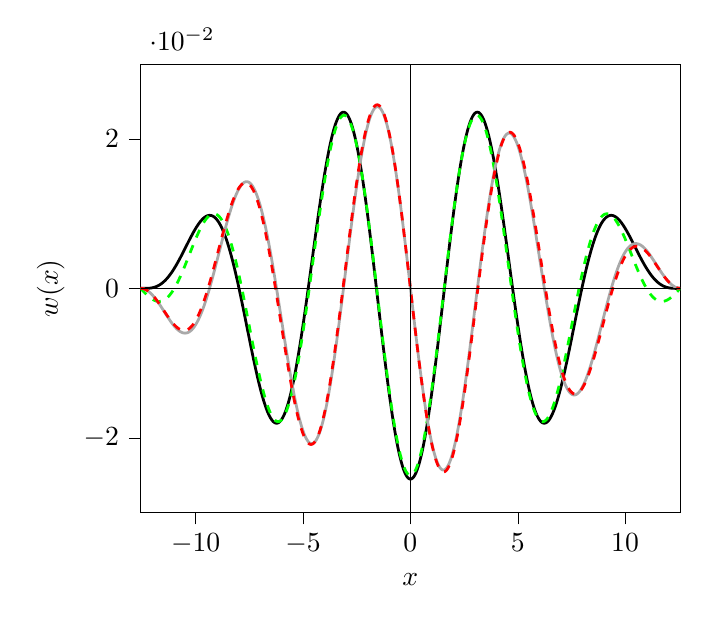
\begin{tikzpicture}

\definecolor{darkgray}{RGB}{169,169,169}
\definecolor{darkgray176}{RGB}{176,176,176}

\begin{axis}[
tick align=outside,
tick pos=left,
x grid style={darkgray176},
xlabel={\(\displaystyle x\)},
xmin=-12.5663706143592, xmax=12.5663706143592,
xtick style={color=black},
y grid style={darkgray176},
ylabel={\(\displaystyle w(x)\)},
ymin=-0.03, ymax=0.03,
ytick style={color=black}
]
\addplot [line width=1pt, black]
table {%
-12.5663706143592 0
-12.5463706143592 -1.18049301471451e-07
-12.5263706143592 -4.37966505707027e-07
-12.5063706143592 -9.0828694165573e-07
-12.4863706143592 -1.47742173070005e-06
-12.4663706143592 -2.0937002910945e-06
-12.4463706143592 -2.70541289398071e-06
-12.4263706143592 -3.26085324413985e-06
-12.4063706143592 -3.70836105849396e-06
-12.3863706143592 -3.99636461600522e-06
-12.3663706143592 -4.07342325142552e-06
-12.3463706143592 -3.88826976643384e-06
-12.3263706143592 -3.38985273148858e-06
-12.3063706143592 -2.52737865150997e-06
-12.2863706143592 -1.25035396861776e-06
-12.2663706143592 4.91373124247887e-07
-12.2463706143592 2.74757108541751e-06
-12.2263706143592 5.56758366892641e-06
-12.2063706143592 9.00028883685626e-06
-12.1863706143592 1.30940579661e-05
-12.1663706143592 1.78967153751e-05
-12.1463706143592 2.34554981965e-05
-12.1263706143592 2.9817016621e-05
-12.1063706143592 3.70272145374e-05
-12.0863706143592 4.51313305945e-05
-12.0663706143592 5.41738597095e-05
-12.0463706143592 6.41985150463e-05
-12.0263706143592 7.52481904902e-05
-12.0063706143592 8.73649236403e-05
-11.9863706143592 0.0001005898593461
-11.9663706143592 0.0001149632138088
-11.9463706143592 0.0001305242392729
-11.9263706143592 0.0001473111893289
-11.9063706143592 0.0001653612848509
-11.8863706143592 0.0001847106805899
-11.8663706143592 0.000205394432445
-11.8463706143592 0.0002274464654343
-11.8263706143592 0.0002508995423848
-11.8063706143592 0.0002757852333631
-11.7863706143592 0.0003021338858666
-11.7663706143592 0.0003299745957942
-11.7463706143592 0.000359335179216
-11.7263706143592 0.0003902421449611
-11.7063706143592 0.00042272066804
-11.6863706143592 0.0004567945639222
-11.6663706143592 0.0004924862636829
-11.6463706143592 0.0005298167900381
-11.6263706143592 0.0005688057342828
-11.6063706143592 0.0006094712341484
-11.5863706143592 0.0006518299525952
-11.5663706143592 0.0006958970575526
-11.5463706143592 0.0007416862026239
-11.5263706143592 0.0007892095087662
-11.5063706143592 0.0008384775469607
-11.4863706143592 0.0008894993218849
-11.4663706143592 0.0009422822565975
-11.4463706143592 0.0009968321782491
-11.4263706143592 0.0010531533048281
-11.4063706143592 0.0011112482329517
-11.3863706143592 0.0011711179267121
-11.3663706143592 0.001232761707586
-11.3463706143592 0.0012961772454168
-11.3263706143592 0.0013613605504745
-11.3063706143592 0.0014283059666039
-11.2863706143592 0.0014970061654635
-11.2663706143592 0.0015674521418642
-11.2463706143592 0.0016396332102102
-11.2263706143592 0.0017135370020481
-11.2063706143592 0.001789149464727
-11.1863706143592 0.0018664548611735
-11.1663706143592 0.0019454357707833
-11.1463706143592 0.0020260730914314
-11.1263706143592 0.0021083460426022
-11.1063706143592 0.0021922321696402
-11.0863706143592 0.0022777073491202
-11.0663706143592 0.0023647457953373
-11.0463706143592 0.0024533200679141
-11.0263706143592 0.0025434010805241
-11.0063706143592 0.0026349581107274
-10.9863706143592 0.0027279588109161
-10.9663706143592 0.0028223692203646
-10.9463706143592 0.0029181537783805
-10.9263706143592 0.0030152753385506
-10.9063706143592 0.0031136951840754
-10.8863706143592 0.0032133730441868
-10.8663706143592 0.0033142671116393
-10.8463706143592 0.0034163340612696
-10.8263706143592 0.0035195290696131
-10.8063706143592 0.00362380583557
-10.7863706143592 0.0037291166021112
-10.7663706143592 0.0038354121790112
-10.7463706143592 0.0039426419665999
-10.7263706143592 0.0040507539805195
-10.7063706143592 0.004159694877475
-10.6863706143592 0.004269409981965
-10.6663706143592 0.0043798433139796
-10.6463706143592 0.0044909376176512
-10.6263706143592 0.004602634390843
-10.6063706143592 0.0047148739156611
-10.5863706143592 0.0048275952898729
-10.5663706143592 0.0049407364592167
-10.5463706143592 0.005054234250585
-10.5263706143592 0.0051680244060637
-10.5063706143592 0.00528204161781
-10.4863706143592 0.00539621956375
-10.4663706143592 0.0055104909440771
-10.4463706143592 0.0056247875185315
-10.4263706143592 0.0057390401444412
-10.4063706143592 0.0058531788155035
-10.3863706143592 0.0059671327012869
-10.3663706143592 0.0060808301874308
-10.3463706143592 0.0061941989165219
-10.3263706143592 0.0063071658296255
-10.3063706143592 0.0064196572084475
-10.2863706143592 0.0065315987181057
-10.2663706143592 0.0066429154504858
-10.2463706143592 0.0067535319681579
-10.2263706143592 0.0068633723488312
-10.2063706143592 0.0069723602303197
-10.1863706143592 0.0070804188559952
-10.1663706143592 0.0071874711207034
-10.1463706143592 0.0072934396171148
-10.1263706143592 0.0073982466824871
-10.1063706143592 0.0075018144458115
-10.0863706143592 0.0076040648753165
-10.0663706143592 0.0077049198263028
-10.0463706143592 0.0078043010892824
-10.0263706143592 0.0079021304383938
-10.0063706143592 0.0079983296800674
-9.98637061435917 0.0080928207019119
-9.96637061435917 0.0081855255217943
-9.94637061435917 0.0082763663370865
-9.92637061435917 0.0083652655740488
-9.90637061435917 0.0084521459373228
-9.88637061435917 0.0085369304595058
-9.86637061435917 0.0086195425507765
-9.84637061435917 0.0086999060485452
-9.82637061435917 0.0087779452670986
-9.80637061435917 0.0088535850472108
-9.78637061435917 0.0089267508056913
-9.76637061435917 0.0089973685848424
-9.74637061435917 0.0090653651017948
-9.72637061435917 0.0091306677976951
-9.70637061435917 0.0091932048867144
-9.68637061435917 0.0092529054048499
-9.66637061435917 0.009309699258491
-9.64637061435917 0.0093635172727206
-9.62637061435917 0.009414291239323
-9.60637061435917 0.0094619539644705
-9.58637061435917 0.0095064393160591
-9.56637061435917 0.0095476822706667
-9.54637061435917 0.0095856189601032
-9.52637061435917 0.0096201867175272
-9.50637061435917 0.0096513241230989
-9.48637061435917 0.009678971049144
-9.46637061435917 0.009703068704799
-9.44637061435917 0.0097235596801115
-9.42637061435917 0.0097403879895698
-9.40637061435917 0.0097534991150321
-9.38637061435917 0.009762840048032
-9.36637061435917 0.0097683593314322
-9.34637061435917 0.0097700071004005
-9.32637061435917 0.0097677351226837
-9.30637061435917 0.0097614968381533
-9.28637061435917 0.0097512473975977
-9.26637061435917 0.0097369437007374
-9.24637061435917 0.0097185444334381
-9.22637061435917 0.0096960101040984
-9.20637061435917 0.0096693030791887
-9.18637061435917 0.0096383876179171
-9.16637061435917 0.0096032299060022
-9.14637061435917 0.0095637980885278
-9.12637061435917 0.0095200623018599
-9.10637061435917 0.0094719947046035
-9.08637061435917 0.0094195695075794
-9.06637061435917 0.0093627630027997
-9.04637061435917 0.0093015535914234
-9.02637061435917 0.009235921810671
-9.00637061435917 0.0091658503596819
-8.98637061435917 0.0090913241242941
-8.96637061435917 0.0090123302007291
-8.94637061435917 0.0089288579181662
-8.92637061435917 0.0088408988601877
-8.90637061435917 0.0087484468850802
-8.88637061435917 0.0086514981449761
-8.86637061435917 0.0085500511038208
-8.84637061435917 0.0084441065541517
-8.82637061435917 0.0083336676326737
-8.80637061435917 0.0082187398346209
-8.78637061435917 0.0080993310268897
-8.76637061435917 0.0079754514599331
-8.74637061435917 0.0078471137784041
-8.72637061435917 0.0077143330305393
-8.70637061435917 0.0075771266762704
-8.68637061435917 0.0074355145940576
-8.66637061435917 0.0072895190864336
-8.64637061435917 0.0071391648842527
-8.62637061435917 0.0069844791496361
-8.60637061435917 0.0068254914776087
-8.58637061435917 0.00666223389642
-8.56637061435917 0.0064947408665458
-8.54637061435917 0.006323049278365
-8.52637061435917 0.0061471984485085
-8.50637061435917 0.0059672301148778
-8.48637061435917 0.0057831884303299
-8.46637061435917 0.0055951199550283
-8.44637061435917 0.0054030736474583
-8.42637061435917 0.0052071008541077
-8.40637061435917 0.005007255297812
-8.38637061435917 0.0048035930647676
-8.36637061435917 0.004596172590213
-8.34637061435917 0.004385054642782
-8.32637061435917 0.0041703023075329
-8.30637061435917 0.0039519809676567
-8.28637061435917 0.0037301582848701
-8.26637061435917 0.0035049041784989
-8.24637061435917 0.0032762908032586
-8.22637061435917 0.0030443925257384
-8.20637061435917 0.0028092858995973
-8.18637061435917 0.0025710496394809
-8.16637061435917 0.0023297645936672
-8.14637061435917 0.002085513715453
-8.12637061435917 0.0018383820332899
-8.10637061435917 0.0015884566196821
-8.08637061435917 0.001335826558859
-8.06637061435917 0.0010805829132326
-8.04637061435917 0.0008228186886568
-8.02637061435917 0.000562628798499
-8.00637061435917 0.0003001100265422
-7.98637061435917 3.53609887304e-05
-7.96637061435917 -0.0002315179062253
-7.94637061435917 -0.0005004244973639
-7.92637061435917 -0.0007712549130963
-7.90637061435917 -0.0010439036139152
-7.88637061435917 -0.0013182634361739
-7.86637061435917 -0.0015942256369144
-7.84637061435917 -0.0018716799397253
-7.82637061435917 -0.0021505145816094
-7.80637061435917 -0.0024306163608389
-7.78637061435917 -0.0027118706857776
-7.76637061435917 -0.0029941616246476
-7.74637061435917 -0.0032773719562179
-7.72637061435917 -0.0035613832213906
-7.70637061435917 -0.0038460757756627
-7.68637061435917 -0.0041313288424372
-7.66637061435917 -0.0044170205671608
-7.64637061435917 -0.0047030280722604
-7.62637061435917 -0.0049892275128544
-7.60637061435917 -0.0052754941332118
-7.58637061435917 -0.0055617023239323
-7.56637061435917 -0.0058477256798204
-7.54637061435917 -0.0061334370584256
-7.52637061435917 -0.0064187086392201
-7.50637061435917 -0.0067034119833874
-7.48637061435917 -0.0069874180941901
-7.46637061435917 -0.0072705974778902
-7.44637061435917 -0.0075528202051902
-7.42637061435917 -0.0078339559731674
-7.40637061435917 -0.0081138741676678
-7.38637061435917 -0.0083924439261321
-7.36637061435917 -0.0086695342008212
-7.34637061435917 -0.00894501382241
-7.32637061435917 -0.0092187515639187
-7.30637061435917 -0.0094906162049488
-7.28637061435917 -0.0097604765961931
-7.26637061435917 -0.0100282017241857
-7.24637061435917 -0.0102936607762618
-7.22637061435917 -0.0105567232056921
-7.20637061435917 -0.0108172587969613
-7.18637061435917 -0.0110751377311559
-7.16637061435917 -0.0113302306514293
-7.14637061435917 -0.0115824087285109
-7.12637061435917 -0.0118315437262243
-7.10637061435917 -0.012077508066984
-7.08637061435917 -0.0123201748972338
-7.06637061435917 -0.012559418152796
-7.04637061435917 -0.012795112624096
-7.02637061435917 -0.0130271340212296
-7.00637061435917 -0.013255359038839
-6.98637061435917 -0.0134796654207634
-6.96637061435917 -0.0136999320244319
-6.94637061435917 -0.0139160388849629
-6.92637061435917 -0.0141278672789395
-6.90637061435917 -0.014335299787824
-6.88637061435917 -0.0145382203609813
-6.86637061435917 -0.0147365143782756
-6.84637061435917 -0.0149300687122091
-6.82637061435917 -0.015118771789568
-6.80637061435917 -0.0153025136525451
-6.78637061435917 -0.0154811860193039
-6.76637061435917 -0.0156546823439544
-6.74637061435917 -0.0158228978759065
-6.72637061435917 -0.0159857297185698
-6.70637061435917 -0.016143076887368
-6.68637061435917 -0.0162948403670369
-6.66637061435917 -0.0164409231681741
-6.64637061435917 -0.0165812303830102
-6.62637061435917 -0.0167156692403703
-6.60637061435917 -0.0168441491597968
-6.58637061435917 -0.0169665818048022
-6.56637061435917 -0.0170828811352235
-6.54637061435917 -0.0171929634586493
-6.52637061435917 -0.0172967474808892
-6.50637061435917 -0.0173941543554593
-6.48637061435917 -0.0174851077320554
-6.46637061435917 -0.0175695338039853
-6.44637061435917 -0.0176473613545349
-6.42637061435917 -0.0177185218022405
-6.40637061435917 -0.017782949245042
-6.38637061435917 -0.0178405805032915
-6.36637061435917 -0.0178913551615911
-6.34637061435917 -0.0179352156094381
-6.32637061435917 -0.0179721070806506
-6.30637061435917 -0.0180019776915526
-6.28637061435917 -0.0180247784778949
-6.26637061435917 -0.0180404634304889
-6.24637061435917 -0.0180489895295337
-6.22637061435917 -0.0180503167776133
-6.20637061435917 -0.0180444082313449
-6.18637061435917 -0.0180312300316586
-6.16637061435917 -0.0180107514326885
-6.14637061435917 -0.0179829448292577
-6.12637061435917 -0.017947785782939
-6.10637061435917 -0.0179052530466742
-6.08637061435917 -0.0178553285879356
-6.06637061435917 -0.0177979976104146
-6.04637061435917 -0.0177332485742209
-6.02637061435917 -0.0176610732145795
-6.00637061435917 -0.0175814665590118
-5.98637061435917 -0.0174944269429862
-5.96637061435917 -0.0173999560240289
-5.94637061435917 -0.0172980587942806
-5.92637061435917 -0.0171887435914907
-5.90637061435917 -0.0170720221084383
-5.88637061435917 -0.0169479094007702
-5.86637061435917 -0.0168164238932489
-5.84637061435917 -0.0166775873844022
-5.82637061435917 -0.0165314250495675
-5.80637061435917 -0.0163779654423256
-5.78637061435917 -0.0162172404943174
-5.76637061435917 -0.0160492855134413
-5.74637061435917 -0.0158741391804248
-5.72637061435917 -0.0156918435437703
-5.70637061435917 -0.0155024440130711
-5.68637061435917 -0.0153059893506971
-5.66637061435917 -0.0151025316618501
-5.64637061435917 -0.0148921263829885
-5.62637061435917 -0.0146748322686233
-5.60637061435917 -0.0144507113764863
-5.58637061435917 -0.014219829051075
-5.56637061435917 -0.0139822539055763
-5.54637061435917 -0.013738057802174
-5.52637061435917 -0.0134873158307463
-5.50637061435917 -0.0132301062859575
-5.48637061435917 -0.0129665106427528
-5.46637061435917 -0.0126966135302619
-5.44637061435917 -0.0124205027041222
-5.42637061435917 -0.0121382690172287
-5.40637061435917 -0.0118500063889218
-5.38637061435917 -0.0115558117726243
-5.36637061435917 -0.0112557851219383
-5.34637061435917 -0.0109500293552147
-5.32637061435917 -0.0106386503186094
-5.30637061435917 -0.0103217567476391
-5.28637061435917 -0.009999460227252
-5.26637061435917 -0.0096718751504294
-5.24637061435917 -0.0093391186753333
-5.22637061435917 -0.0090013106810188
-5.20637061435917 -0.0086585737217269
-5.18637061435917 -0.0083110329797791
-5.16637061435917 -0.0079588162170898
-5.14637061435917 -0.0076020537253191
-5.12637061435917 -0.0072408782746857
-5.10637061435917 -0.0068754250614612
-5.08637061435917 -0.0065058316541678
-5.06637061435917 -0.0061322379385029
-5.04637061435917 -0.0057547860610132
-5.02637061435917 -0.0053736203715432
-5.00637061435917 -0.0049888873644819
-4.98637061435917 -0.004600735618834
-4.96637061435917 -0.0042093157371409
-4.94637061435917 -0.0038147802832796
-4.92637061435917 -0.0034172837191637
-4.90637061435917 -0.0030169823403783
-4.88637061435917 -0.002614034210774
-4.86637061435917 -0.0022085990960504
-4.84637061435917 -0.0018008383963586
-4.82637061435917 -0.0013909150779524
-4.80637061435917 -0.0009789936039193
-4.78637061435917 -0.0005652398640213
-4.76637061435917 -0.0001498211036789
-4.74637061435917 0.0002670941478716
-4.72637061435917 0.0006853361502138
-4.70637061435917 0.0011047340251462
-4.68637061435917 0.0015251158308058
-4.66637061435917 0.0019463086364829
-4.64637061435917 0.0023681385980959
-4.62637061435917 0.0027904310342898
-4.60637061435917 0.0032130105031232
-4.58637061435917 0.0036357008793103
-4.56637061435917 0.0040583254319799
-4.54637061435917 0.0044807069029171
-4.52637061435917 0.0049026675852505
-4.50637061435917 0.0053240294025486
-4.48637061435917 0.005744613988289
-4.46637061435917 0.0061642427656619
-4.44637061435917 0.0065827370276727
-4.42637061435917 0.0069999180175036
-4.40637061435917 0.0074156070090993
-4.38637061435917 0.0078296253879365
-4.36637061435917 0.0082417947319398
-4.34637061435917 0.0086519368925072
-4.32637061435917 0.0090598740756045
-4.30637061435917 0.0094654289228919
-4.28637061435917 0.009868424592844
-4.26637061435917 0.0102686848418241
-4.24637061435917 0.0106660341050741
-4.22637061435917 0.0110602975775826
-4.20637061435917 0.0114513012947909
-4.18637061435917 0.0118388722130994
-4.16637061435917 0.0122228382901353
-4.14637061435917 0.0126030285647427
-4.12637061435917 0.0129792732366583
-4.10637061435917 0.0133514037458314
-4.08637061435917 0.0137192528513525
-4.06637061435917 0.0140826547099513
-4.04637061435917 0.014441444954026
-4.02637061435917 0.014795460769166
-4.00637061435917 0.0151445409711304
-3.98637061435917 0.0154885260822455
-3.96637061435917 0.0158272584071826
-3.94637061435917 0.0161605821080803
-3.92637061435917 0.016488343278974
-3.90637061435917 0.0168103900194965
-3.88637061435917 0.0171265725078124
-3.86637061435917 0.0174367430727523
-3.84637061435917 0.0177407562651093
-3.82637061435917 0.0180384689280634
-3.80637061435917 0.0183297402666998
-3.78637061435917 0.0186144319165848
-3.76637061435917 0.0188924080113668
-3.74637061435917 0.0191635352493679
-3.72637061435917 0.0194276829591332
-3.70637061435917 0.019684723163905
-3.68637061435917 0.0199345306449894
-3.66637061435917 0.020176983003984
-3.64637061435917 0.0204119607238342
-3.62637061435917 0.020639347228689
-3.60637061435917 0.0208590289425246
-3.58637061435917 0.0210708953465063
-3.56637061435917 0.0212748390350607
-3.54637061435917 0.0214707557706274
-3.52637061435917 0.021658544537065
-3.50637061435917 0.0218381075916809
-3.48637061435917 0.022009350515861
-3.46637061435917 0.0221721822642711
-3.44637061435917 0.0223265152126056
-3.42637061435917 0.0224722652038578
-3.40637061435917 0.0226093515930891
-3.38637061435917 0.0227376972906716
-3.36637061435917 0.0228572288039828
-3.34637061435917 0.02296787627753
-3.32637061435917 0.023069573531483
-3.30637061435917 0.0231622580985937
-3.28637061435917 0.0232458712594842
-3.26637061435917 0.0233203580762831
-3.24637061435917 0.023385667424592
-3.22637061435917 0.0234417520237648
-3.20637061435917 0.0234885684654825
-3.18637061435917 0.023526077240608
-3.16637061435917 0.0235542427643057
-3.14637061435917 0.0235730333994102
-3.12637061435917 0.0235824214780334
-3.10637061435917 0.0235823833213932
-3.08637061435917 0.0235728992578559
-3.06637061435917 0.023553953639178
-3.04637061435917 0.0235255348549397
-3.02637061435917 0.0234876353451582
-3.00637061435917 0.0234402516110743
-2.98637061435917 0.0233833842241039
-2.96637061435917 0.023317037832947
-2.94637061435917 0.023241221168849
-2.92637061435917 0.0231559470490091
-2.90637061435917 0.0230612323781311
-2.88637061435917 0.0229570981481139
-2.86637061435917 0.0228435694358787
-2.84637061435917 0.022720675399332
-2.82637061435917 0.0225884492714628
-2.80637061435917 0.022446928352575
-2.78637061435917 0.0222961540006561
-2.76637061435917 0.022136171619883
-2.74637061435917 0.0219670306472701
-2.72637061435917 0.0217887845374602
-2.70637061435917 0.0216014907456667
-2.68637061435917 0.0214052107087684
-2.66637061435917 0.0212000098245678
-2.64637061435917 0.0209859574292158
-2.62637061435917 0.0207631267728147
-2.60637061435917 0.0205315949932058
-2.58637061435917 0.0202914430879533
-2.56637061435917 0.020042755884534
-2.54637061435917 0.0197856220087461
-2.52637061435917 0.0195201338513469
-2.50637061435917 0.0192463875329363
-2.48637061435917 0.018964482867097
-2.46637061435917 0.0186745233218083
-2.44637061435917 0.0183766159791493
-2.42637061435917 0.0180708714933073
-2.40637061435917 0.0177574040469099
-2.38637061435917 0.017436331305698
-2.36637061435917 0.017107774371561
-2.34637061435917 0.0167718577339509
-2.32637061435917 0.0164287092196989
-2.30637061435917 0.016078459941255
-2.28637061435917 0.0157212442433721
-2.26637061435917 0.0153571996482589
-2.24637061435917 0.0149864667992245
-2.22637061435917 0.0146091894028397
-2.20637061435917 0.0142255141696398
-2.18637061435917 0.0138355907533953
-2.16637061435917 0.0134395716889769
-2.14637061435917 0.013037612328842
-2.12637061435917 0.0126298707781712
-2.10637061435917 0.0122165078286831
-2.08637061435917 0.0117976868911565
-2.06637061435917 0.0113735739266908
-2.04637061435917 0.0109443373767342
-2.02637061435917 0.0105101480919117
-2.00637061435917 0.0100711792596844
-1.98637061435917 0.0096276063308719
-1.96637061435917 0.0091796069450719
-1.94637061435917 0.0087273608550099
-1.92637061435917 0.0082710498498522
-1.90637061435917 0.0078108576775186
-1.88637061435917 0.0073469699660277
-1.86637061435917 0.0068795741439122
-1.84637061435917 0.0064088593597391
-1.82637061435917 0.005935016400771
-1.80637061435917 0.005458237610807
-1.78637061435917 0.0049787168072382
-1.76637061435917 0.0044966491973572
-1.74637061435917 0.0040122312939594
-1.72637061435917 0.0035256608302735
-1.70637061435917 0.0030371366742612
-1.68637061435917 0.0025468587423249
-1.66637061435917 0.0020550279124623
-1.64637061435917 0.0015618459369077
-1.62637061435917 0.0010675153543008
-1.60637061435917 0.0005722394014219
-1.58637061435917 7.62219245357e-05
-1.56637061435917 -0.000420332709618
-1.54637061435917 -0.000917219703144
-1.52637061435917 -0.0014142339165809
-1.50637061435917 -0.0019111699587193
-1.48637061435917 -0.0024078222766078
-1.46637061435917 -0.0029039852457047
-1.44637061435917 -0.0033994532601342
-1.42637061435917 -0.0038940208230053
-1.40637061435917 -0.0043874826367523
-1.38637061435917 -0.0048796336934547
-1.36637061435917 -0.0053702693650949
-1.34637061435917 -0.0058591854937119
-1.32637061435917 -0.0063461784814097
-1.30637061435917 -0.0068310453801787
-1.28637061435917 -0.0073135839814879
-1.26637061435917 -0.0077935929056075
-1.24637061435917 -0.008270871690619
-1.22637061435917 -0.0087452208810742
-1.20637061435917 -0.009216442116258
-1.18637061435917 -0.0096843382180186
-1.16637061435917 -0.0101487132781202
-1.14637061435917 -0.0106093727450809
-1.12637061435917 -0.0110661235104537
-1.10637061435917 -0.0115187739945104
-1.08637061435917 -0.0119671342312898
-1.06637061435917 -0.0124110159529696
-1.04637061435917 -0.0128502326735232
-1.02637061435917 -0.0132845997716227
-1.00637061435917 -0.0137139345727482
-0.986370614359172 -0.0141380564304674
-0.966370614359173 -0.0145567868068456
-0.946370614359172 -0.0149699493519498
-0.926370614359172 -0.0153773699824091
-0.906370614359172 -0.0157788769589957
-0.886370614359173 -0.0161743009631893
-0.866370614359171 -0.0165634751726899
-0.846370614359172 -0.0169462353358432
-0.826370614359172 -0.017322419844945
-0.806370614359173 -0.0176918698083883
-0.786370614359173 -0.0180544291216218
-0.766370614359172 -0.018409944536885
-0.746370614359172 -0.0187582657316876
-0.726370614359173 -0.0190992453760022
-0.706370614359173 -0.0194327391981371
-0.686370614359172 -0.0197586060492606
-0.666370614359172 -0.0200767079665444
-0.646370614359173 -0.0203869102348981
-0.626370614359173 -0.0206890814472655
-0.606370614359172 -0.0209830935634544
-0.586370614359172 -0.0212688219674721
-0.566370614359172 -0.0215461455233402
-0.546370614359173 -0.0218149466293629
-0.526370614359172 -0.0220751112708222
-0.506370614359172 -0.0223265290710761
-0.486370614359172 -0.0225690933410366
-0.466370614359173 -0.0228027011270025
-0.446370614359171 -0.0230272532568263
-0.426370614359172 -0.0232426543843927
-0.406370614359172 -0.0234488130323876
-0.386370614359173 -0.023645641633339
-0.366370614359171 -0.0238330565689083
-0.346370614359172 -0.0240109782074159
-0.326370614359172 -0.0241793309395819
-0.306370614359173 -0.0243380432124656
-0.286370614359171 -0.0244870475615883
-0.266370614359172 -0.024626280641224
-0.246370614359172 -0.0247556832528433
-0.226370614359173 -0.0248752003716981
-0.206370614359173 -0.0249847811715342
-0.186370614359172 -0.0250843790474198
-0.166370614359172 -0.0251739516366801
-0.146370614359173 -0.025253460837927
-0.126370614359173 -0.0253228728281765
-0.106370614359172 -0.0253821580780437
-0.086370614359172 -0.0254312913650109
-0.0663706143591724 -0.0254702517847597
-0.0463706143591728 -0.0254990227605643
-0.0263706143591715 -0.02551759205074
-0.0063706143591719 -0.0255259517541439
0.0136293856408276 -0.0255240983137254
0.0336293856408271 -0.0255120325181248
0.0536293856408285 -0.0254897595013185
0.0736293856408281 -0.0254572887403124
0.0936293856408276 -0.0254146340508832
0.113629385640827 -0.02536181358137
0.133629385640829 -0.0252988498045203
0.153629385640828 -0.0252257695073919
0.173629385640828 -0.0251426037793175
0.193629385640827 -0.0250493879979369
0.213629385640829 -0.0249461618133028
0.233629385640828 -0.024832969130069
0.253629385640828 -0.0247098580877678
0.273629385640827 -0.0245768810391871
0.293629385640827 -0.0244340945268568
0.313629385640828 -0.024281559257655
0.333629385640828 -0.0241193400755478
0.353629385640827 -0.0239475059324725
0.373629385640827 -0.0237661298573812
0.393629385640828 -0.0235752889234564
0.413629385640828 -0.023375064213516
0.433629385640827 -0.0231655407836226
0.453629385640827 -0.0229468076249156
0.473629385640828 -0.0227189576236817
0.493629385640828 -0.0224820875196858
0.513629385640828 -0.0222362978627781
0.533629385640827 -0.0219816929678009
0.553629385640829 -0.0217183808678144
0.573629385640828 -0.0214464732656643
0.593629385640828 -0.0211660854839131
0.613629385640827 -0.0208773364131589
0.633629385640829 -0.0205803484587671
0.653629385640828 -0.0202752474860376
0.673629385640828 -0.0199621627638348
0.693629385640827 -0.0196412269067068
0.713629385640829 -0.0193125758155201
0.733629385640828 -0.0189763486166383
0.753629385640828 -0.0186326875996722
0.773629385640827 -0.0182817381538325
0.793629385640827 -0.0179236487029121
0.813629385640828 -0.0175585706389308
0.833629385640828 -0.0171866582544723
0.853629385640827 -0.0168080686737444
0.873629385640827 -0.0164229617823971
0.893629385640828 -0.0160315001561283
0.913629385640828 -0.0156338489881129
0.933629385640828 -0.0152301760152874
0.953629385640827 -0.0148206514435261
0.973629385640828 -0.0144054478717422
0.993629385640828 -0.0139847402149506
1.01362938564083 -0.0135587056263269
1.03362938564083 -0.0131275234183006
1.05362938564083 -0.0126913749827176
1.07362938564083 -0.0122504437101104
1.09362938564083 -0.0118049149081129
1.11362938564083 -0.0113549757190588
1.13362938564083 -0.0109008150368
1.15362938564083 -0.0104426234227863
1.17362938564083 -0.0099805930214436
1.19362938564083 -0.0095149174748896
1.21362938564083 -0.0090457918370294
1.23362938564083 -0.0085734124870672
1.25362938564083 -0.0080979770424772
1.27362938564083 -0.0076196842714727
1.29362938564083 -0.0071387340050145
1.31362938564083 -0.0066553270483988
1.33362938564083 -0.0061696650924671
1.35362938564083 -0.005681950624477
1.37362938564083 -0.0051923868386773
1.39362938564083 -0.0047011775466279
1.41362938564083 -0.0042085270873057
1.43362938564083 -0.0037146402370384
1.45362938564083 -0.0032197221193085
1.47362938564083 -0.0027239781144682
1.49362938564083 -0.0022276137694069
1.51362938564083 -0.0017308347072143
1.53362938564083 -0.0012338465368788
1.55362938564083 -0.0007368547630646
1.57362938564083 -0.0002400646960086
1.59362938564083 0.0002563186384228
1.61362938564083 0.0007520905884735
1.63362938564083 0.0012470469659937
1.65362938564083 0.0017409841356518
1.67362938564083 0.0022336991038197
1.69362938564083 0.0027249896070926
1.71362938564083 0.0032146542004004
1.73362938564083 0.0037024923446723
1.75362938564083 0.0041883044940136
1.77362938564083 0.0046718921823553
1.79362938564083 0.0051530581095357
1.81362938564083 0.0056316062267765
1.83362938564083 0.0061073418215132
1.85362938564083 0.0065800716015413
1.87362938564083 0.0070496037784402
1.89362938564083 0.0075157481502373
1.91362938564083 0.0079783161832734
1.93362938564083 0.008437121093234
1.95362938564083 0.0088919779253082
1.97362938564083 0.0093427036334406
1.99362938564083 0.0097891171586384
2.01362938564083 0.0102310395062997
2.03362938564083 0.0106682938225286
2.05362938564083 0.0111007054694006
2.07362938564083 0.0115281020991473
2.09362938564083 0.0119503137272243
2.11362938564083 0.0123671728042321
2.13362938564083 0.0127785142866557
2.15362938564083 0.0131841757063931
2.17362938564083 0.0135839972390404
2.19362938564083 0.0139778217709036
2.21362938564083 0.0143654949647079
2.23362938564083 0.014746865323974
2.25362938564083 0.015121784256035
2.27362938564083 0.0154901061336641
2.29362938564083 0.0158516883552873
2.31362938564083 0.016206391403754
2.33362938564083 0.0165540789036401
2.35362938564083 0.0168946176770596
2.37362938564083 0.0172278777979576
2.39362938564083 0.017553732644865
2.41362938564083 0.0178720589520888
2.43362938564083 0.0181827368593183
2.45362938564083 0.0184856499596248
2.47362938564083 0.0187806853458345
2.49362938564083 0.0190677336552551
2.51362938564083 0.019346689112738
2.53362938564083 0.0196174495720559
2.55362938564083 0.0198799165555819
2.57362938564083 0.0201339952922496
2.59362938564083 0.0203795947537827
2.61362938564083 0.0206166276891761
2.63362938564083 0.0208450106574171
2.65362938564083 0.0210646640584315
2.67362938564083 0.0212755121622442
2.69362938564083 0.0214774831363414
2.71362938564083 0.0216705090712258
2.73362938564083 0.0218545260041533
2.75362938564083 0.0220294739410431
2.77362938564083 0.0221952968765548
2.79362938564083 0.0223519428123227
2.81362938564083 0.022499363773344
2.83362938564083 0.0226375158225136
2.85362938564083 0.0227663590733031
2.87362938564083 0.0228858577005783
2.89362938564083 0.0229959799495548
2.91362938564083 0.0230966981428886
2.93362938564083 0.0231879886859018
2.95362938564083 0.023269832069943
2.97362938564083 0.0233422128738835
2.99362938564083 0.0234051197637512
3.01362938564083 0.0234585454905052
3.03362938564083 0.0235024868859546
3.05362938564083 0.0235369448568259
3.07362938564083 0.0235619243769842
3.09362938564083 0.0235774344778152
3.11362938564083 0.0235834882367748
3.13362938564083 0.0235801027641136
3.15362938564083 0.0235672991877865
3.17362938564083 0.0235451026365559
3.19362938564083 0.0235135422212997
3.21362938564083 0.0234726510145358
3.23362938564083 0.023422466028174
3.25362938564083 0.0233630281895103
3.27362938564083 0.0232943823154759
3.29362938564083 0.0232165770851561
3.31362938564083 0.0231296650105953
3.33362938564083 0.0230337024059029
3.35362938564083 0.0229287493546793
3.37362938564083 0.0228148696757774
3.39362938564083 0.0226921308874205
3.41362938564083 0.0225606041696947
3.43362938564083 0.0224203643254359
3.45362938564083 0.0222714897395334
3.47362938564083 0.0221140623366708
3.49362938564083 0.021948167537526
3.51362938564083 0.0217738942134552
3.53362938564083 0.021591334639683
3.55362938564083 0.0214005844470234
3.57362938564083 0.0212017425721569
3.59362938564083 0.0209949112064901
3.61362938564083 0.0207801957436229
3.63362938564083 0.0205577047254507
3.65362938564083 0.020327549786931
3.67362938564083 0.0200898455995387
3.69362938564083 0.0198447098134438
3.71362938564083 0.0195922629984366
3.73362938564083 0.0193326285836328
3.75362938564083 0.0190659327959884
3.77362938564083 0.0187923045976552
3.79362938564083 0.0185118756222082
3.81362938564083 0.0182247801097777
3.83362938564083 0.0179311548411179
3.85362938564083 0.0176311390706449
3.87362938564083 0.0173248744584781
3.89362938564083 0.0170125050015182
3.91362938564083 0.0166941769635961
3.93362938564083 0.016370038804728
3.95362938564083 0.0160402411095106
3.97362938564083 0.0157049365146926
3.99362938564083 0.0153642796359577
4.01362938564083 0.0150184269939555
4.03362938564083 0.0146675369396166
4.05362938564083 0.0143117695787875
4.07362938564083 0.0139512866962237
4.09362938564083 0.0135862516789777
4.11362938564083 0.0132168294392178
4.13362938564083 0.0128431863365176
4.15362938564083 0.0124654900996521
4.17362938564083 0.0120839097479391
4.19362938564083 0.0116986155121644
4.21362938564083 0.0113097787551271
4.23362938564083 0.010917571891847
4.25362938564083 0.0105221683094681
4.27362938564083 0.0101237422869001
4.29362938564083 0.0097224689142354
4.31362938564083 0.0093185240119794
4.33362938564083 0.008912084050134
4.35362938564083 0.0085033260671724
4.37362938564083 0.008092427588944
4.39362938564083 0.0076795665475473
4.41362938564083 0.0072649212002106
4.43362938564083 0.0068486700482182
4.45362938564083 0.0064309917559203
4.47362938564083 0.0060120650698658
4.49362938564083 0.005592068738095
4.51362938564083 0.0051711814296309
4.53362938564083 0.0047495816542077
4.55362938564083 0.0043274476822715
4.57362938564083 0.0039049574652947
4.59362938564083 0.0034822885564373
4.61362938564083 0.003059618031595
4.63362938564083 0.0026371224108695
4.65362938564083 0.0022149775804976
4.67362938564083 0.0017933587152759
4.69362938564083 0.0013724402015161
4.71362938564083 0.0009523955605673
4.73362938564083 0.0005333973729402
4.75362938564083 0.0001156172030675
4.77362938564083 -0.0003007744752636
4.79362938564083 -0.000715608352775
4.81362938564083 -0.0011287163578203
4.83362938564083 -0.0015399317287371
4.85362938564083 -0.0019490890853928
4.87362938564083 -0.0023560244998938
4.89362938564083 -0.0027605755664251
4.91362938564083 -0.0031625814701887
4.93362938564083 -0.0035618830554108
4.95362938564083 -0.0039583228923871
4.97362938564083 -0.0043517453435349
4.99362938564083 -0.0047419966284258
5.01362938564083 -0.0051289248877665
5.03362938564083 -0.0055123802463023
5.05362938564083 -0.0058922148746146
5.07362938564083 -0.0062682830497855
5.09362938564083 -0.0066404412149025
5.11362938564083 -0.0070085480373788
5.13362938564083 -0.0073724644660625
5.15362938564083 -0.0077320537871121
5.17362938564083 -0.0080871816786118
5.19362938564083 -0.0084377162639062
5.21362938564083 -0.0087835281636296
5.23362938564083 -0.0091244905464098
5.25362938564083 -0.0094604791782238
5.27362938564083 -0.0097913724703859
5.29362938564083 -0.0101170515261481
5.31362938564083 -0.0104374001858943
5.33362938564083 -0.0107523050709086
5.35362938564083 -0.0110616556257022
5.37362938564083 -0.0113653441588804
5.39362938564083 -0.0116632658825349
5.41362938564083 -0.0119553189501444
5.43362938564083 -0.0122414044929718
5.45362938564083 -0.0125214266549409
5.47362938564083 -0.0127952926259823
5.49362938564083 -0.013062912673835
5.51362938564083 -0.0133242001742928
5.53362938564083 -0.0135790716398842
5.55362938564083 -0.0138274467469772
5.57362938564083 -0.0140692483612986
5.59362938564083 -0.014304402561861
5.61362938564083 -0.0145328386632883
5.63362938564083 -0.0147544892365355
5.65362938564083 -0.0149692901279942
5.67362938564083 -0.0151771804769819
5.69362938564083 -0.0153781027316074
5.71362938564083 -0.015572002663013
5.73362938564083 -0.0157588293779869
5.75362938564083 -0.015938535329947
5.77362938564083 -0.0161110763282941
5.79362938564083 -0.016276411546134
5.81362938564083 -0.0164345035263701
5.83362938564083 -0.0165853181861672
5.85362938564083 -0.0167288248197893
5.87362938564083 -0.0168649960998144
5.89362938564083 -0.0169938080767299
5.91362938564083 -0.017115240176914
5.93362938564083 -0.0172292751990079
5.95362938564083 -0.0173358993086849
5.97362938564083 -0.0174351020318254
5.99362938564083 -0.017526876246102
6.01362938564083 -0.0176112181709878
6.03362938564083 -0.0176881273561928
6.05362938564083 -0.0177576066685426
6.07362938564083 -0.0178196622773073
6.09362938564083 -0.0178743036379934
6.11362938564083 -0.0179215434746117
6.13362938564083 -0.0179613977604335
6.15362938564083 -0.0179938856972484
6.17362938564083 -0.0180190296931401
6.19362938564083 -0.0180368553387937
6.21362938564083 -0.0180473913823511
6.23362938564083 -0.0180506697028318
6.25362938564083 -0.0180467252821351
6.27362938564083 -0.018035596175643
6.29362938564083 -0.0180173234814416
6.31362938564083 -0.017991951308181
6.33362938564083 -0.0179595267415927
6.35362938564083 -0.0179200998096861
6.37362938564083 -0.0178737234466449
6.39362938564083 -0.0178204534554449
6.41362938564083 -0.0177603484692158
6.43362938564083 -0.0176934699113704
6.45362938564083 -0.0176198819545239
6.47362938564083 -0.017539651478228
6.49362938564083 -0.0174528480255441
6.51362938564083 -0.0173595437584811
6.53362938564083 -0.0172598134123229
6.55362938564083 -0.0171537342488724
6.57362938564083 -0.0170413860086379
6.59362938564083 -0.0169228508619901
6.61362938564083 -0.0167982133593156
6.63362938564083 -0.0166675603801966
6.65362938564083 -0.0165309810816442
6.67362938564083 -0.0163885668454147
6.69362938564083 -0.0162404112244371
6.71362938564083 -0.0160866098883828
6.73362938564083 -0.0159272605684068
6.75362938564083 -0.01576246300109
6.77362938564083 -0.0155923188716147
6.79362938564083 -0.0154169317562029
6.81362938564083 -0.0152364070638493
6.83362938564083 -0.015050851977381
6.85362938564083 -0.014860375393874
6.87362938564083 -0.0146650878644607
6.89362938564083 -0.0144651015335587
6.91362938564083 -0.0142605300775551
6.93362938564083 -0.0140514886429775
6.95362938564083 -0.0138380937841853
6.97362938564083 -0.0136204634006144
6.99362938564083 -0.0133987166736081
7.01362938564083 -0.0131729740028672
7.03362938564083 -0.012943356942554
7.05362938564083 -0.0127099881370819
7.07362938564083 -0.0124729912566251
7.09362938564083 -0.0122324909323826
7.11362938564083 -0.0119886126916287
7.13362938564083 -0.0117414828925845
7.15362938564083 -0.0114912286591448
7.17362938564083 -0.0112379778154919
7.19362938564083 -0.0109818588206328
7.21362938564083 -0.0107230007028904
7.23362938564083 -0.0104615329943849
7.25362938564083 -0.0101975856655367
7.27362938564083 -0.0099312890596257
7.29362938564083 -0.0096627738274393
7.31362938564083 -0.0093921708620423
7.33362938564083 -0.0091196112337021
7.35362938564083 -0.0088452261250013
7.37362938564083 -0.0085691467661712
7.39362938564083 -0.0082915043706773
7.41362938564083 -0.0080124300710903
7.43362938564083 -0.0077320548552736
7.45362938564083 -0.0074505095029196
7.47362938564083 -0.0071679245224657
7.49362938564083 -0.0068844300884212
7.51362938564083 -0.006600155979137
7.53362938564083 -0.0063152315150468
7.55362938564083 -0.0060297854974114
7.57362938564083 -0.0057439461475957
7.59362938564083 -0.0054578410469075
7.61362938564083 -0.0051715970770277
7.63362938564083 -0.0048853403610602
7.65362938564083 -0.0045991962052305
7.67362938564083 -0.0043132890412604
7.69362938564083 -0.0040277423694464
7.71362938564083 -0.0037426787024687
7.73362938564083 -0.0034582195099585
7.75362938564083 -0.0031744851638477
7.77362938564083 -0.0028915948845294
7.79362938564083 -0.0026096666878512
7.81362938564083 -0.0023288173329691
7.83362938564083 -0.0020491622710839
7.85362938564083 -0.0017708155950846
7.87362938564083 -0.001493889990122
7.89362938564083 -0.0012184966851352
7.91362938564083 -0.0009447454053517
7.93362938564083 -0.0006727443257845
7.95362938564083 -0.000402600025745
7.97362938564083 -0.0001344174443943
7.99362938564083 0.0001317001626507
8.01362938564083 0.0003956512656338
8.03362938564083 0.0006573361018829
8.05362938564083 0.0009166567159212
8.07362938564083 0.0011735169984495
8.09362938564083 0.0014278227241828
8.11362938564083 0.0016794815885259
8.13362938564083 0.0019284032430718
8.15362938564083 0.0021744993299096
8.17362938564083 0.0024176835147274
8.19362938564083 0.0026578715186964
8.21362938564083 0.0028949811491253
8.23362938564083 0.0031289323288715
8.25362938564083 0.0033596471244991
8.27362938564083 0.0035870497731726
8.29362938564083 0.0038110667082769
8.31362938564083 0.0040316265837553
8.33362938564083 0.0042486602971546
8.35362938564083 0.0044621010113736
8.37362938564083 0.0046718841751046
8.39362938564083 0.0048779475419638
8.41362938564083 0.0050802311883037
8.43362938564083 0.0052786775297049
8.45362938564083 0.0054732313361402
8.47362938564083 0.005663839745811
8.49362938564083 0.0058504522776503
8.51362938564083 0.0060330208424934
8.53362938564083 0.0062114997529127
8.55362938564083 0.0063858457317175
8.57362938564083 0.0065560179191188
8.59362938564083 0.00672197787856
8.61362938564083 0.0068836896012155
8.63362938564083 0.0070411195091594
8.65362938564083 0.0071942364572073
8.67362938564083 0.007343011733435
8.69362938564083 0.00748741905838
8.71362938564083 0.0076274345829287
8.73362938564083 0.0077630368848971
8.75362938564083 0.0078942069643112
8.77362938564083 0.0080209282373937
8.79362938564083 0.0081431865292659
8.81362938564083 0.0082609700653735
8.83362938564083 0.0083742694616446
8.85362938564083 0.0084830777133908
8.87362938564083 0.0085873901829623
8.89362938564083 0.0086872045861673
8.91362938564083 0.0087825209774684
8.93362938564083 0.0088733417339688
8.95362938564083 0.0089596715382001
8.97362938564083 0.009041517359728
8.99362938564083 0.0091188884355874
9.01362938564083 0.0091917962495642
9.03362938564083 0.0092602545103388
9.05362938564083 0.0093242791285065
9.07362938564083 0.0093838881924933
9.09362938564083 0.009439101943383
9.11362938564083 0.0094899427486741
9.13362938564083 0.0095364350749848
9.15362938564083 0.0095786054597253
9.17362938564083 0.0096164824817567
9.19362938564083 0.0096500967310556
9.21362938564083 0.0096794807774072
9.23362938564083 0.0097046691381447
9.25362938564083 0.0097256982449591
9.27362938564083 0.0097426064098001
9.29362938564083 0.0097554337898901
9.31362938564083 0.0097642223518749
9.33362938564083 0.0097690158351336
9.35362938564083 0.0097698597142718
9.37362938564083 0.0097668011608212
9.39362938564083 0.0097598890041715
9.41362938564083 0.0097491736917572
9.43362938564083 0.0097347072485259
9.45362938564083 0.0097165432357138
9.47362938564083 0.0096947367089519
9.49362938564083 0.0096693441757315
9.51362938564083 0.0096404235522535
9.53362938564083 0.0096080341196894
9.55362938564083 0.0095722364798793
9.57362938564083 0.0095330925104954
9.59362938564083 0.0094906653196976
9.61362938564083 0.009445019200309
9.63362938564083 0.0093962195835389
9.65362938564083 0.0093443329922808
9.67362938564083 0.0092894269940141
9.69362938564083 0.0092315701533384
9.71362938564083 0.009170831984166
9.73362938564083 0.009107282901605
9.75362938564083 0.0090409941735581
9.77362938564083 0.008972037872068
9.79362938564083 0.008900486824437
9.81362938564083 0.0088264145641506
9.83362938564083 0.0087498952816324
9.85362938564083 0.0086710037748614
9.87362938564083 0.0085898153998782
9.89362938564083 0.0085064060212107
9.91362938564083 0.0084208519622474
9.93362938564083 0.008333229955588
9.95362938564083 0.0082436170933979
9.97362938564083 0.0081520907777981
9.99362938564083 0.0080587286713175
10.0136293856408 0.0079636086474359
10.0336293856408 0.0078668087412471
10.0536293856408 0.0077684071002697
10.0736293856408 0.0076684819354338
10.0936293856408 0.0075671114722719
10.1136293856408 0.0074643739023408
10.1336293856408 0.0073603473349039
10.1536293856408 0.0072551097488988
10.1736293856408 0.0071487389452201
10.1936293856408 0.0070413124993417
10.2136293856408 0.0069329077143071
10.2336293856408 0.0068236015741133
10.2536293856408 0.0067134706975145
10.2736293856408 0.0066025912922716
10.2936293856408 0.0064910391098726
10.3136293856408 0.0063788894007499
10.3336293856408 0.006266216870018
10.3536293856408 0.0061530956337575
10.3736293856408 0.0060395991758687
10.3936293856408 0.0059258003055187
10.4136293856408 0.0058117711152058
10.4336293856408 0.0056975829394629
10.4536293856408 0.0055833063142248
10.4736293856408 0.0054690109368784
10.4936293856408 0.0053547656270205
10.5136293856408 0.0052406382879425
10.5336293856408 0.0051266958688633
10.5536293856408 0.0050130043279309
10.5736293856408 0.0048996285960129
10.5936293856408 0.0047866325412936
10.6136293856408 0.0046740789346989
10.6336293856408 0.0045620294161654
10.6536293856408 0.0044505444617723
10.6736293856408 0.0043396833517532
10.6936293856408 0.0042295041394051
10.7136293856408 0.0041200636209093
10.7336293856408 0.0040114173060817
10.7536293856408 0.0039036193900663
10.7736293856408 0.0037967227259864
10.7936293856408 0.0036907787985684
10.8136293856408 0.0035858376987498
10.8336293856408 0.0034819480992868
10.8536293856408 0.0033791572313699
10.8736293856408 0.0032775108622629
10.8936293856408 0.0031770532739735
10.9136293856408 0.0030778272429665
10.9336293856408 0.0029798740209303
10.9536293856408 0.0028832333166036
10.9736293856408 0.0027879432786735
10.9936293856408 0.0026940404797496
11.0136293856408 0.0026015599014243
11.0336293856408 0.0025105349204232
11.0536293856408 0.0024209972958533
11.0736293856408 0.0023329771575529
11.0936293856408 0.0022465029955489
11.1136293856408 0.002161601650624
11.1336293856408 0.0020782983059987
11.1536293856408 0.0019966164801288
11.1736293856408 0.0019165780206218
11.1936293856408 0.0018382030992732
11.2136293856408 0.0017615102082224
11.2336293856408 0.001686516157229
11.2536293856408 0.0016132360720688
11.2736293856408 0.001541683394048
11.2936293856408 0.0014718698806326
11.3136293856408 0.0014038056071925
11.3336293856408 0.0013374989698547
11.3536293856408 0.0012729566894629
11.3736293856408 0.001210183816639
11.3936293856408 0.0011491837379404
11.4136293856408 0.0010899581831076
11.4336293856408 0.0010325072333963
11.4536293856408 0.0009768293309855
11.4736293856408 0.0009229212894548
11.4936293856408 0.0008707783053222
11.5136293856408 0.0008203939706337
11.5336293856408 0.0007717602865939
11.5536293856408 0.0007248676782297
11.5736293856408 0.000679705010073
11.5936293856408 0.0006362596028547
11.6136293856408 0.0005945172511948
11.6336293856408 0.0005544622422779
11.6536293856408 0.0005160773755001
11.6736293856408 0.0004793439830744
11.6936293856408 0.0004442419515797
11.7136293856408 0.0004107497444381
11.7336293856408 0.0003788444253069
11.7536293856408 0.0003485016823675
11.7736293856408 0.000319695853496
11.7936293856408 0.0002923999522986
11.8136293856408 0.0002665856949936
11.8336293856408 0.0002422235281225
11.8536293856408 0.0002192826570733
11.8736293856408 0.000197731075394
11.8936293856408 0.0001775355948802
11.9136293856408 0.0001586618764158
11.9336293856408 0.0001410744615459
11.9536293856408 0.0001247368047625
11.9736293856408 0.0001096113064821
11.9936293856408 9.56593466923e-05
12.0136293856408 8.28413192477e-05
12.0336293856408 7.11166667916e-05
12.0536293856408 6.04439162807e-05
12.0736293856408 5.07807150923e-05
12.0936293856408 4.20838676872e-05
12.1136293856408 3.43093728083e-05
12.1336293856408 2.74124611887e-05
12.1536293856408 2.1347633747e-05
12.1736293856408 1.60687002434e-05
12.1936293856408 1.15288183743e-05
12.2136293856408 7.68053327853233e-06
12.2336293856408 4.47581743123133e-06
12.2536293856408 1.86611089987179e-06
12.2736293856408 -1.97638063433489e-07
12.2936293856408 -1.76493211897124e-06
12.3136293856408 -2.88568365146433e-06
12.3336293856408 -3.61017332333983e-06
12.3536293856408 -3.98900839572929e-06
12.3736293856408 -4.07308084307948e-06
12.3936293856408 -3.91352528804236e-06
12.4136293856408 -3.5616767834999e-06
12.4336293856408 -3.06902846790255e-06
12.4536293856408 -2.48718912094387e-06
12.4736293856408 -1.86784064636394e-06
12.4936293856408 -1.26269550873991e-06
12.5136293856408 -7.23454150815014e-07
12.5336293856408 -3.01762418752584e-07
12.5536293856408 -4.91690217154214e-08
};
\addplot [line width=1pt, green, dashed]
table {%
-12.5663706143592 -1.53304261083376e-18
-12.5463706143592 -6.25786315286e-05
-12.5263706143592 -0.000125081775314
-12.5063706143592 -0.0001874339952431
-12.4863706143592 -0.0002495599584326
-12.4663706143592 -0.0003113844867688
-12.4463706143592 -0.0003728326083561
-12.4263706143592 -0.0004338296088447
-12.4063706143592 -0.000494301082608
-12.3863706143592 -0.0005541729837386
-12.3663706143592 -0.0006133716768335
-12.3463706143592 -0.0006718239875389
-12.3263706143592 -0.0007294572528248
-12.3063706143592 -0.0007861993709599
-12.2863706143592 -0.0008419788511572
-12.2663706143592 -0.0008967248628616
-12.2463706143592 -0.0009503672846501
-12.2263706143592 -0.0010028367527165
-12.2063706143592 -0.0010540647089112
-12.1863706143592 -0.0011039834483083
-12.1663706143592 -0.0011525261662723
-12.1463706143592 -0.0011996270049961
-12.1263706143592 -0.0012452210994827
-12.1063706143592 -0.0012892446229446
-12.0863706143592 -0.0013316348315925
-12.0663706143592 -0.001372330108788
-12.0463706143592 -0.0014112700085337
-12.0263706143592 -0.0014483952982747
-12.0063706143592 -0.0014836480009866
-11.9863706143592 -0.0015169714365249
-11.9663706143592 -0.0015483102622103
-11.9463706143592 -0.0015776105126274
-11.9263706143592 -0.0016048196386113
-11.9063706143592 -0.0016298865454001
-11.8863706143592 -0.0016527616299295
-11.8663706143592 -0.001673396817248
-11.8463706143592 -0.0016917455960299
-11.8263706143592 -0.0017077630531654
-11.8063706143592 -0.0017214059074067
-11.7863706143592 -0.0017326325420496
-11.7663706143592 -0.0017414030366304
-11.7463706143592 -0.0017476791976205
-11.7263706143592 -0.001751424588097
-11.7063706143592 -0.0017526045563741
-11.6863706143592 -0.001751186263576
-11.6663706143592 -0.0017471387101343
-11.6463706143592 -0.0017404327611942
-11.6263706143592 -0.0017310411709135
-11.6063706143592 -0.0017189386056384
-11.5863706143592 -0.0017041016659422
-11.5663706143592 -0.0016865089075132
-11.5463706143592 -0.0016661408608777
-11.5263706143592 -0.0016429800499453
-11.5063706143592 -0.001617011009366
-11.4863706143592 -0.0015882203006856
-11.4663706143592 -0.0015565965272898
-11.4463706143592 -0.0015221303481275
-11.4263706143592 -0.0014848144902023
-11.4063706143592 -0.0014446437598248
-11.3863706143592 -0.001401615052618
-11.3663706143592 -0.0013557273622661
-11.3463706143592 -0.0013069817880037
-11.3263706143592 -0.0012553815408361
-11.3063706143592 -0.0012009319484875
-11.2863706143592 -0.0011436404590722
-11.2663706143592 -0.0010835166434838
-11.2463706143592 -0.0010205721965016
-11.2263706143592 -0.0009548209366096
-11.2063706143592 -0.0008862788045275
-11.1863706143592 -0.0008149638604527
-11.1663706143592 -0.000740896280013
-11.1463706143592 -0.0006640983489302
-11.1263706143592 -0.0005845944563963
-11.1063706143592 -0.0005024110871637
-11.0863706143592 -0.0004175768123527
-11.0663706143592 -0.0003301222789791
-11.0463706143592 -0.0002400801982059
-11.0263706143592 -0.0001474853323244
-11.0063706143592 -5.23744804702e-05
-10.9863706143592 4.52135369203e-05
-10.9663706143592 0.0001452378949059
-10.9463706143592 0.00024765578208
-10.9263706143592 0.0003524224198472
-10.9063706143592 0.0004594910829275
-10.8863706143592 0.0005688131210764
-10.8663706143592 0.0006803379820142
-10.8463706143592 0.0007940132355493
-10.8263706143592 0.0009097845988872
-10.8063706143592 0.0010275959631104
-10.7863706143592 0.0011473894208178
-10.7663706143592 0.0012691052949084
-10.7463706143592 0.0013926821684958
-10.7263706143592 0.0015180569159382
-10.7063706143592 0.0016451647349683
-10.6863706143592 0.0017739391799064
-10.6663706143592 0.0019043121959403
-10.6463706143592 0.0020362141544545
-10.6263706143592 0.0021695738893892
-10.6063706143592 0.0023043187346125
-10.5863706143592 0.0024403745622851
-10.5663706143592 0.002577665822197
-10.5463706143592 0.0027161155820584
-10.5263706143592 0.0028556455687197
-10.5063706143592 0.0029961762103034
-10.4863706143592 0.0031376266792223
-10.4663706143592 0.0032799149360633
-10.4463706143592 0.0034229577743135
-10.4263706143592 0.003566670865904
-10.4063706143592 0.0037109688075484
-10.3863706143592 0.0038557651678508
-10.3663706143592 0.0040009725351587
-10.3463706143592 0.0041465025661343
-10.3263706143592 0.0042922660350202
-10.3063706143592 0.0044381728835712
-10.2863706143592 0.0045841322716263
-10.2663706143592 0.0047300526282942
-10.2463706143592 0.004875841703724
-10.2263706143592 0.0050214066214336
-10.2063706143592 0.005166653931168
-10.1863706143592 0.0053114896622578
-10.1663706143592 0.0054558193774502
-10.1463706143592 0.0055995482271831
-10.1263706143592 0.0057425810042722
-10.1063706143592 0.0058848221989818
-10.0863706143592 0.00602617605445
-10.0663706143592 0.0061665466224363
-10.0463706143592 0.0063058378193633
-10.0263706143592 0.0064439534826203
-10.0063706143592 0.0065807974270983
-9.98637061435917 0.0067162735019259
-9.96637061435917 0.0068502856473743
-9.94637061435917 0.0069827379519003
-9.92637061435917 0.0071135347092961
-9.90637061435917 0.0072425804759138
-9.88637061435917 0.0073697801279331
-9.86637061435917 0.0074950389186415
-9.84637061435917 0.0076182625356929
-9.82637061435917 0.0077393571583155
-9.80637061435917 0.0078582295144349
-9.78637061435917 0.0079747869376822
-9.76637061435917 0.0080889374242537
-9.74637061435917 0.0082005896895916
-9.72637061435917 0.008309653224854
-9.70637061435917 0.0084160383531407
-9.68637061435917 0.0085196562854456
-9.66637061435917 0.0086204191763021
-9.64637061435917 0.0087182401790915
-9.62637061435917 0.008813033500982
-9.60637061435917 0.0089047144574682
-9.58637061435917 0.0089931995264785
-9.56637061435917 0.0090784064020218
-9.54637061435917 0.0091602540473406
-9.52637061435917 0.0092386627475418
-9.50637061435917 0.0093135541616735
-9.48637061435917 0.0093848513742199
-9.46637061435917 0.009452478945982
-9.44637061435917 0.0095163629643168
-9.42637061435917 0.0095764310927051
-9.40637061435917 0.0096326126196187
-9.38637061435917 0.0096848385066596
-9.36637061435917 0.0097330414359415
-9.34637061435917 0.0097771558566872
-9.32637061435917 0.0098171180310143
-9.30637061435917 0.0098528660788807
-9.28637061435917 0.0098843400221656
-9.26637061435917 0.0099114818278577
-9.24637061435917 0.0099342354503261
-9.22637061435917 0.0099525468726479
-9.20637061435917 0.0099663641469679
-9.18637061435917 0.0099756374338662
-9.16637061435917 0.0099803190407088
-9.14637061435917 0.009980363458959
-9.12637061435917 0.0099757274004262
-9.10637061435917 0.009966369832429
-9.08637061435917 0.0099522520118522
-9.06637061435917 0.0099333375180747
-9.04637061435917 0.0099095922847494
-9.02637061435917 0.0098809846304128
-9.00637061435917 0.0098474852879068
-8.98637061435917 0.0098090674325926
-8.96637061435917 0.0097657067093377
-8.94637061435917 0.0097173812582602
-8.92637061435917 0.0096640717392112
-8.90637061435917 0.0096057613549798
-8.88637061435917 0.0095424358732051
-8.86637061435917 0.0094740836469794
-8.84637061435917 0.0094006956341277
-8.82637061435917 0.0093222654151515
-8.80637061435917 0.0092387892098212
-8.78637061435917 0.0091502658924063
-8.76637061435917 0.0090566970055316
-8.74637061435917 0.0089580867726473
-8.72637061435917 0.0088544421091033
-8.70637061435917 0.0087457726318183
-8.68637061435917 0.0086320906675341
-8.66637061435917 0.0085134112596473
-8.64637061435917 0.0083897521736111
-8.62637061435917 0.0082611339008999
-8.60637061435917 0.0081275796615314
-8.58637061435917 0.0079891154051406
-8.56637061435917 0.0078457698106009
-8.54637061435917 0.0076975742841895
-8.52637061435917 0.0075445629562934
-8.50637061435917 0.0073867726766537
-8.48637061435917 0.0072242430081478
-8.46637061435917 0.0070570162191076
-8.44637061435917 0.0068851372741741
-8.42637061435917 0.0067086538236904
-8.40637061435917 0.0065276161916329
-8.38637061435917 0.0063420773620849
-8.36637061435917 0.0061520929642541
-8.34637061435917 0.0059577212560397
-8.32637061435917 0.0057590231061526
-8.30637061435917 0.0055560619747943
-8.28637061435917 0.0053489038929011
-8.26637061435917 0.005137617439961
-8.24637061435917 0.0049222737204103
-8.22637061435917 0.0047029463386182
-8.20637061435917 0.0044797113724707
-8.18637061435917 0.0042526473455606
-8.16637061435917 0.0040218351979981
-8.14637061435917 0.0037873582558498
-8.12637061435917 0.0035493021992221
-8.10637061435917 0.0033077550289984
-8.08637061435917 0.0030628070322471
-8.06637061435917 0.0028145507463123
-8.04637061435917 0.002563080921604
-8.02637061435917 0.002308494483103
-8.00637061435917 0.0020508904905968
-7.98637061435917 0.0017903700976654
-7.96637061435917 0.0015270365094322
-7.94637061435917 0.0012609949391012
-7.92637061435917 0.0009923525632986
-7.90637061435917 0.000721218476239
-7.88637061435917 0.0004477036427365
-7.86637061435917 0.0001719208500831
-7.84637061435917 -0.0001060153411855
-7.82637061435917 -0.0003859886476131
-7.80637061435917 -0.000667881114211
-7.78637061435917 -0.0009515731668896
-7.76637061435917 -0.0012369436659076
-7.74637061435917 -0.001523869960314
-7.72637061435917 -0.0018122279433577
-7.70637061435917 -0.0021018921088392
-7.68637061435917 -0.0023927356083766
-7.66637061435917 -0.0026846303095602
-7.64637061435917 -0.0029774468549672
-7.62637061435917 -0.003271054722009
-7.60637061435917 -0.0035653222835819
-7.58637061435917 -0.0038601168694926
-7.56637061435917 -0.0041553048286293
-7.54637061435917 -0.0044507515918475
-7.52637061435917 -0.0047463217355408
-7.50637061435917 -0.0050418790458664
-7.48637061435917 -0.0053372865835926
-7.46637061435917 -0.0056324067495383
-7.44637061435917 -0.0059271013505718
-7.42637061435917 -0.0062212316661366
-7.40637061435917 -0.0065146585152713
-7.38637061435917 -0.0068072423240923
-7.36637061435917 -0.0070988431937033
-7.34637061435917 -0.0073893209685003
-7.32637061435917 -0.0076785353048377
-7.30637061435917 -0.007966345740021
-7.28637061435917 -0.0082526117615921
-7.26637061435917 -0.0085371928768727
-7.24637061435917 -0.0088199486827312
-7.22637061435917 -0.0091007389355379
-7.20637061435917 -0.0093794236212736
-7.18637061435917 -0.0096558630257564
-7.16637061435917 -0.0099299178049513
-7.14637061435917 -0.0102014490553274
-7.12637061435917 -0.0104703183842261
-7.10637061435917 -0.0107363879802065
-7.08637061435917 -0.0109995206833307
-7.06637061435917 -0.0112595800553535
-7.04637061435917 -0.0115164304497819
-7.02637061435917 -0.0117699370817669
-7.00637061435917 -0.0120199660977931
-6.98637061435917 -0.0122663846451306
-6.96637061435917 -0.0125090609410114
-6.94637061435917 -0.0127478643414978
-6.92637061435917 -0.012982665410005
-6.90637061435917 -0.0132133359854429
-6.88637061435917 -0.0134397492499426
-6.86637061435917 -0.0136617797961314
-6.84637061435917 -0.0138793036939227
-6.82637061435917 -0.0140921985567838
-6.80637061435917 -0.0143003436074495
-6.78637061435917 -0.0145036197430451
-6.76637061435917 -0.0147019095995854
-6.74637061435917 -0.0148950976158163
-6.72637061435917 -0.0150830700963643
-6.70637061435917 -0.0152657152741605
-6.68637061435917 -0.0154429233721076
-6.66637061435917 -0.0156145866639551
-6.64637061435917 -0.0157805995343514
-6.62637061435917 -0.0159408585380405
-6.60637061435917 -0.0160952624581717
-6.58637061435917 -0.0162437123636903
-6.56637061435917 -0.0163861116657793
-6.54637061435917 -0.0165223661733211
-6.52637061435917 -0.016652384147349
-6.50637061435917 -0.0167760763544593
-6.48637061435917 -0.016893356119154
-6.46637061435917 -0.0170041393750863
-6.44637061435917 -0.0171083447151807
-6.42637061435917 -0.0172058934405991
-6.40637061435917 -0.0172967096085264
-6.38637061435917 -0.017380720078749
-6.36637061435917 -0.0174578545590003
-6.34637061435917 -0.0175280456490467
-6.32637061435917 -0.0175912288834904
-6.30637061435917 -0.0176473427732642
-6.28637061435917 -0.0176963288457942
-6.26637061435917 -0.0177381316838077
-6.24637061435917 -0.0177726989627642
-6.22637061435917 -0.0177999814868867
-6.20637061435917 -0.0178199332237729
-6.18637061435917 -0.0178325113375657
-6.16637061435917 -0.017837676220663
-6.14637061435917 -0.0178353915239477
-6.12637061435917 -0.0178256241855197
-6.10637061435917 -0.0178083444579116
-6.08637061435917 -0.0177835259337725
-6.06637061435917 -0.0177511455700012
-6.04637061435917 -0.0177111837103166
-6.02637061435917 -0.0176636241062467
-6.00637061435917 -0.0176084539365261
-5.98637061435917 -0.0175456638248857
-5.96637061435917 -0.0174752478562233
-5.94637061435917 -0.0173972035911441
-5.92637061435917 -0.0173115320788592
-5.90637061435917 -0.0172182378684317
-5.88637061435917 -0.0171173290183627
-5.86637061435917 -0.0170088171045072
-5.84637061435917 -0.0168927172263129
-5.82637061435917 -0.0167690480113743
-5.80637061435917 -0.0166378316182977
-5.78637061435917 -0.0164990937378701
-5.76637061435917 -0.0163528635925282
-5.74637061435917 -0.0161991739341245
-5.72637061435917 -0.0160380610399874
-5.70637061435917 -0.0158695647072731
-5.68637061435917 -0.0156937282456086
-5.66637061435917 -0.0155105984680257
-5.64637061435917 -0.0153202256801863
-5.62637061435917 -0.0151226636679013
-5.60637061435917 -0.0149179696829439
-5.58637061435917 -0.0147062044271622
-5.56637061435917 -0.0144874320348943
-5.54637061435917 -0.0142617200536902
-5.52637061435917 -0.014029139423348
-5.50637061435917 -0.0137897644532685
-5.48637061435917 -0.0135436727981382
-5.46637061435917 -0.0132909454319469
-5.44637061435917 -0.0130316666203497
-5.42637061435917 -0.0127659238913839
-5.40637061435917 -0.0124938080045504
-5.38637061435917 -0.0122154129182723
-5.36637061435917 -0.0119308357557416
-5.34637061435917 -0.0116401767691693
-5.32637061435917 -0.0113435393024505
-5.30637061435917 -0.011041029752261
-5.28637061435917 -0.0107327575276007
-5.26637061435917 -0.0104188350077993
-5.24637061435917 -0.0100993774990025
-5.22637061435917 -0.0097745031891559
-5.20637061435917 -0.0094443331015061
-5.18637061435917 -0.0091089910466374
-5.16637061435917 -0.0087686035730652
-5.14637061435917 -0.0084232999164065
-5.12637061435917 -0.0080732119471497
-5.10637061435917 -0.0077184741170455
-5.08637061435917 -0.0073592234041424
-5.06637061435917 -0.0069955992564907
-5.04637061435917 -0.0066277435345386
-5.02637061435917 -0.0062558004522477
-5.00637061435917 -0.0058799165169508
-4.98637061435917 -0.0055002404679812
-4.96637061435917 -0.0051169232140988
-4.94637061435917 -0.0047301177697419
-4.92637061435917 -0.0043399791901325
-4.90637061435917 -0.0039466645052644
-4.88637061435917 -0.0035503326528036
-4.86637061435917 -0.003151144409931
-4.84637061435917 -0.0027492623241583
-4.82637061435917 -0.0023448506431487
-4.80637061435917 -0.0019380752435734
-4.78637061435917 -0.0015291035590372
-4.76637061435917 -0.0011181045071054
-4.74637061435917 -0.0007052484154654
-4.72637061435917 -0.000290706947257
-4.70637061435917 0.0001253469743942
-4.68637061435917 0.0005427392426064
-4.66637061435917 0.0009612946436979
-4.64637061435917 0.001380836934835
-4.62637061435917 0.0018011889223371
-4.60637061435917 0.0022221725405992
-4.58637061435917 0.0026436089315993
-4.56637061435917 0.0030653185249504
-4.54637061435917 0.0034871211184619
-4.52637061435917 0.0039088359591711
-4.50637061435917 0.0043302818248085
-4.48637061435917 0.0047512771056579
-4.46637061435917 0.0051716398867727
-4.44637061435917 0.0055911880305103
-4.42637061435917 0.0060097392593449
-4.40637061435917 0.0064271112389216
-4.38637061435917 0.0068431216613095
-4.36637061435917 0.0072575883284177
-4.34637061435917 0.0076703292355318
-4.32637061435917 0.0080811626549336
-4.30637061435917 0.0084899072195631
-4.28637061435917 0.0088963820066824
-4.26637061435917 0.009300406621504
-4.24637061435917 0.0097018012807401
-4.22637061435917 0.0101003868960366
-4.20637061435917 0.0104959851572494
-4.18637061435917 0.0108884186155239
-4.16637061435917 0.0112775107661378
-4.14637061435917 0.0116630861310683
-4.12637061435917 0.0120449703412417
-4.10637061435917 0.0124229902184286
-4.08637061435917 0.0127969738567427
-4.06637061435917 0.0131667507037059
-4.04637061435917 0.0135321516408388
-4.02637061435917 0.0138930090637386
-4.00637061435917 0.0142491569616051
-3.98637061435917 0.0146004309961766
-3.96637061435917 0.014946668580037
-3.94637061435917 0.0152877089542553
-3.92637061435917 0.0156233932653212
-3.90637061435917 0.0159535646413379
-3.88637061435917 0.0162780682674354
-3.86637061435917 0.0165967514603668
-3.84637061435917 0.0169094637422517
-3.82637061435917 0.0172160569134302
-3.80637061435917 0.0175163851243915
-3.78637061435917 0.0178103049467417
-3.76637061435917 0.0180976754431755
-3.74637061435917 0.0183783582364177
-3.72637061435917 0.0186522175771005
-3.70637061435917 0.0189191204105414
-3.68637061435917 0.0191789364423909
-3.66637061435917 0.0194315382031147
-3.64637061435917 0.0196768011112804
-3.62637061435917 0.0199146035356157
-3.60637061435917 0.0201448268558077
-3.58637061435917 0.0203673555220117
-3.56637061435917 0.0205820771130417
-3.54637061435917 0.0207888823932104
-3.52637061435917 0.0209876653677923
-3.50637061435917 0.0211783233370806
-3.48637061435917 0.0213607569490105
-3.46637061435917 0.0215348702503225
-3.44637061435917 0.0217005707362395
-3.42637061435917 0.0218577693986313
-3.40637061435917 0.0220063807726428
-3.38637061435917 0.0221463229817617
-3.36637061435917 0.0222775177813018
-3.34637061435917 0.022399890600279
-3.32637061435917 0.0225133705816596
-3.30637061435917 0.022617890620958
-3.28637061435917 0.0227133874031649
-3.26637061435917 0.0227998014379846
-3.24637061435917 0.0228770770933652
-3.22637061435917 0.0229451626273006
-3.20637061435917 0.0230040102178903
-3.18637061435917 0.0230535759916373
-3.16637061435917 0.0230938200499714
-3.14637061435917 0.0231247064939813
-3.12637061435917 0.0231462034473429
-3.10637061435917 0.0231582830774288
-3.08637061435917 0.0231609216145897
-3.06637061435917 0.0231540993695932
-3.04637061435917 0.0231378007492123
-3.02637061435917 0.0231120142699513
-3.00637061435917 0.0230767325699033
-2.98637061435917 0.0230319524187288
-2.96637061435917 0.0229776747257501
-2.94637061435917 0.0229139045461543
-2.92637061435917 0.0228406510853014
-2.90637061435917 0.0227579277011307
-2.88637061435917 0.0226657519046647
-2.86637061435917 0.0225641453586062
-2.84637061435917 0.0224531338740281
-2.82637061435917 0.0223327474051541
-2.80637061435917 0.0222030200422324
-2.78637061435917 0.0220639900025008
-2.76637061435917 0.0219156996192488
-2.74637061435917 0.0217581953289758
-2.72637061435917 0.0215915276566526
-2.70637061435917 0.0214157511990886
-2.68637061435917 0.0212309246064121
-2.66637061435917 0.0210371105616689
-2.64637061435917 0.0208343757585475
-2.62637061435917 0.0206227908772395
-2.60637061435917 0.0204024305584434
-2.58637061435917 0.0201733733755228
-2.56637061435917 0.0199357018048304
-2.54637061435917 0.0196895021942083
-2.52637061435917 0.0194348647296792
-2.50637061435917 0.0191718834003405
-2.48637061435917 0.0189006559614773
-2.46637061435917 0.0186212838959084
-2.44637061435917 0.0183338723735827
-2.42637061435917 0.0180385302094424
-2.40637061435917 0.0177353698195705
-2.38637061435917 0.0174245071756432
-2.36637061435917 0.0171060617577044
-2.34637061435917 0.0167801565052842
-2.32637061435917 0.0164469177668827
-2.30637061435917 0.0161064752478394
-2.28637061435917 0.0157589619566137
-2.26637061435917 0.0154045141494971
-2.24637061435917 0.015043271273784
-2.22637061435917 0.0146753759094238
-2.20637061435917 0.0143009737091822
-2.18637061435917 0.0139202133373369
-2.16637061435917 0.0135332464069348
-2.14637061435917 0.0131402274156402
-2.12637061435917 0.0127413136802002
-2.10637061435917 0.0123366652695592
-2.08637061435917 0.0119264449366503
-2.06637061435917 0.0115108180488952
-2.04637061435917 0.0110899525174442
-2.02637061435917 0.0106640187251872
-2.00637061435917 0.0102331894535686
-1.98637061435917 0.0097976398082395
-1.96637061435917 0.0093575471435802
-1.94637061435917 0.0089130909861277
-1.92637061435917 0.0084644529569425
-1.90637061435917 0.0080118166929501
-1.88637061435917 0.0075553677672933
-1.86637061435917 0.0070952936087305
-1.84637061435917 0.0066317834201187
-1.82637061435917 0.0061650280960155
-1.80637061435917 0.0056952201394407
-1.78637061435917 0.0052225535778336
-1.76637061435917 0.0047472238782446
-1.74637061435917 0.0042694278618013
-1.72637061435917 0.0037893636174864
-1.70637061435917 0.0033072304152682
-1.68637061435917 0.0028232286186233
-1.66637061435917 0.0023375595964919
-1.64637061435917 0.0018504256347049
-1.62637061435917 0.0013620298469254
-1.60637061435917 0.0008725760851447
-1.58637061435917 0.0003822688497733
-1.56637061435917 -0.0001086868006297
-1.54637061435917 -0.0006000853399501
-1.52637061435917 -0.0010917208653894
-1.50637061435917 -0.0015833871885744
-1.48637061435917 -0.0020748779268618
-1.46637061435917 -0.0025659865947959
-1.44637061435917 -0.0030565066956763
-1.42637061435917 -0.003546231813195
-1.40637061435917 -0.0040349557030992
-1.38637061435917 -0.0045224723848368
-1.36637061435917 -0.005008576233144
-1.34637061435917 -0.0054930620695303
-1.32637061435917 -0.0059757252536204
-1.30637061435917 -0.0064563617743092
-1.28637061435917 -0.0069347683406886
-1.26637061435917 -0.0074107424727026
-1.24637061435917 -0.00788408259149
-1.22637061435917 -0.0083545881093719
-1.20637061435917 -0.0088220595194417
-1.18637061435917 -0.0092862984847172
-1.16637061435917 -0.0097471079268121
-1.14637061435917 -0.010204292114086
-1.12637061435917 -0.0106576567492321
-1.10637061435917 -0.0111070090562618
-1.08637061435917 -0.0115521578668444
-1.06637061435917 -0.011992913705964
-1.04637061435917 -0.0124290888768514
-1.02637061435917 -0.0128604975451525
-1.00637061435917 -0.0132869558222934
-0.986370614359172 -0.0137082818480046
-0.966370614359173 -0.014124295871963
-0.946370614359172 -0.0145348203345171
-0.926370614359172 -0.0149396799464543
-0.906370614359172 -0.0153387017677755
-0.886370614359173 -0.0157317152854392
-0.866370614359171 -0.0161185524900384
-0.846370614359172 -0.0164990479513748
-0.826370614359172 -0.0168730388928957
-0.806370614359173 -0.0172403652649571
-0.786370614359173 -0.0176008698168803
-0.766370614359172 -0.0179543981677675
-0.746370614359172 -0.0183007988760428
-0.726370614359173 -0.0186399235076876
-0.706370614359173 -0.0189716267031368
-0.686370614359172 -0.0192957662428049
-0.666370614359172 -0.0196122031112121
-0.646370614359173 -0.0199208015596794
-0.626370614359173 -0.0202214291675635
-0.606370614359172 -0.0205139569020034
-0.586370614359172 -0.0207982591761495
-0.566370614359172 -0.0210742139058498
-0.546370614359173 -0.0213417025647642
-0.526370614359172 -0.0216006102378831
-0.506370614359172 -0.0218508256734236
-0.486370614359172 -0.0220922413330812
-0.466370614359173 -0.0223247534406101
-0.446370614359171 -0.0225482620287123
-0.426370614359172 -0.0227626709842125
-0.406370614359172 -0.0229678880914965
-0.386370614359173 -0.0231638250741944
-0.366370614359171 -0.0233503976350882
-0.346370614359172 -0.0235275254942246
-0.326370614359172 -0.0236951324252165
-0.306370614359173 -0.0238531462897147
-0.286370614359171 -0.0240014990700341
-0.266370614359172 -0.0241401268999197
-0.246370614359172 -0.0242689700934371
-0.226370614359173 -0.0243879731719741
-0.206370614359173 -0.0244970848893415
-0.186370614359172 -0.0245962582549598
-0.166370614359172 -0.0246854505551224
-0.146370614359173 -0.0247646233723247
-0.126370614359173 -0.0248337426026498
-0.106370614359172 -0.0248927784712026
-0.086370614359172 -0.024941705545586
-0.0663706143591724 -0.0249805027474113
-0.0463706143591728 -0.0250091533618392
-0.0263706143591715 -0.0250276450451448
-0.0063706143591719 -0.0250359698303054
0.0136293856408276 -0.0250341241306067
0.0336293856408271 -0.0250221087412659
0.0536293856408285 -0.0249999288390721
0.0736293856408281 -0.024967593980043
0.0936293856408276 -0.0249251180950992
0.113629385640827 -0.024872519483759
0.133629385640829 -0.024809820805855
0.153629385640828 -0.0247370490712785
0.173629385640828 -0.0246542356277545
0.193629385640827 -0.0245614161466541
0.213629385640829 -0.0244586306068516
0.233629385640828 -0.0243459232766319
0.253629385640828 -0.0242233426936588
0.273629385640827 -0.0240909416430124
0.293629385640827 -0.0239487771333064
0.313629385640828 -0.0237969103708957
0.333629385640828 -0.0236354067321881
0.353629385640827 -0.0234643357340715
0.373629385640827 -0.0232837710024708
0.393629385640828 -0.0230937902390502
0.413629385640828 -0.0228944751860755
0.433629385640827 -0.0226859115894531
0.453629385640827 -0.0224681891599638
0.473629385640828 -0.0222414015327086
0.493629385640828 -0.0220056462247861
0.513629385640828 -0.0217610245912212
0.533629385640827 -0.0215076417791659
0.553629385640829 -0.0212456066803939
0.573629385640828 -0.0209750318821105
0.593629385640828 -0.0206960336161018
0.613629385640827 -0.0204087317062466
0.633629385640829 -0.0201132495144155
0.653629385640828 -0.0198097138847836
0.673629385640828 -0.0194982550865807
0.693629385640827 -0.0191790067553084
0.713629385640829 -0.0188521058324503
0.733629385640828 -0.0185176925037036
0.753629385640828 -0.0181759101357609
0.773629385640827 -0.0178269052116731
0.793629385640827 -0.0174708272648221
0.813629385640828 -0.0171078288115345
0.833629385640828 -0.0167380652823696
0.853629385640827 -0.0163616949521112
0.873629385640827 -0.015978878868498
0.893629385640828 -0.015589780779725
0.913629385640828 -0.0151945670607509
0.933629385640828 -0.0147934066384437
0.953629385640827 -0.0143864709156027
0.973629385640828 -0.0139739336938897
0.993629385640828 -0.0135559710957072
1.01362938564083 -0.0131327614850585
1.03362938564083 -0.0127044853874291
1.05362938564083 -0.0122713254087238
1.07362938564083 -0.0118334661533007
1.09362938564083 -0.0113910941411367
1.11362938564083 -0.0109443977241668
1.13362938564083 -0.0104935670018338
1.15362938564083 -0.0100387937358885
1.17362938564083 -0.0095802712644811
1.19362938564083 -0.0091181944155818
1.21362938564083 -0.0086527594197731
1.23362938564083 -0.0081841638224535
1.25362938564083 -0.0077126063954929
1.27362938564083 -0.0072382870483825
1.29362938564083 -0.0067614067389184
1.31362938564083 -0.006282167383463
1.33362938564083 -0.0058007717668232
1.35362938564083 -0.0053174234517901
1.37362938564083 -0.0048323266883798
1.39362938564083 -0.0043456863228192
1.41362938564083 -0.0038577077063183
1.43362938564083 -0.0033685966036714
1.45362938564083 -0.0028785591017298
1.47362938564083 -0.0023878015177886
1.49362938564083 -0.0018965303079296
1.51362938564083 -0.0014049519753632
1.53362938564083 -0.0009132729788117
1.55362938564083 -0.0004216996409761
1.57362938564083 6.95619428702e-05
1.59362938564083 0.0005603059961208
1.61362938564083 0.0010503271518635
1.63362938564083 0.0015394205436558
1.65362938564083 0.0020273818960055
1.67362938564083 0.0025140076145156
1.69362938564083 0.0029990948756503
1.71362938564083 0.0034824417160826
1.73362938564083 0.0039638471215809
1.75362938564083 0.0044431111153955
1.77362938564083 0.0049200348461011
1.79362938564083 0.0053944206748591
1.81362938564083 0.0058660722620562
1.83362938564083 0.0063347946532811
1.85362938564083 0.0068003943646004
1.87362938564083 0.0072626794670924
1.89362938564083 0.0077214596706035
1.91362938564083 0.0081765464066851
1.93362938564083 0.0086277529106766
1.95362938564083 0.0090748943028942
1.97362938564083 0.0095177876688911
1.99362938564083 0.0099562521387497
2.01362938564083 0.0103901089653724
2.03362938564083 0.0108191816017339
2.05362938564083 0.0112432957770602
2.07362938564083 0.0116622795719
2.09362938564083 0.0120759634920545
2.11362938564083 0.0124841805413321
2.13362938564083 0.0128867662930948
2.15362938564083 0.0132835589605651
2.17362938564083 0.0136743994658605
2.19362938564083 0.0140591315077256
2.21362938564083 0.0144376016279309
2.23362938564083 0.0148096592763084
2.25362938564083 0.0151751568743958
2.27362938564083 0.01553394987766
2.29362938564083 0.015885896836273
2.31362938564083 0.0162308594544122
2.33362938564083 0.0165687026480601
2.35362938564083 0.016899294601277
2.37362938564083 0.0172225068209226
2.39362938564083 0.0175382141898012
2.41362938564083 0.0178462950182088
2.43362938564083 0.0181466310938591
2.45362938564083 0.0184391077301659
2.47362938564083 0.0187236138128618
2.49362938564083 0.0190000418449336
2.51362938564083 0.0192682879898533
2.53362938564083 0.0195282521130884
2.55362938564083 0.0197798378218724
2.57362938564083 0.0200229525032191
2.59362938564083 0.0202575073601653
2.61362938564083 0.0204834174462257
2.63362938564083 0.0207006016980467
2.65362938564083 0.0209089829662457
2.67362938564083 0.0211084880444232
2.69362938564083 0.0212990476963352
2.71362938564083 0.0214805966812169
2.73362938564083 0.0216530737772472
2.75362938564083 0.0218164218031434
2.77362938564083 0.0219705876378815
2.79362938564083 0.0221155222385311
2.81362938564083 0.0222511806562016
2.83362938564083 0.0223775220500927
2.85362938564083 0.0224945096996455
2.87362938564083 0.0226021110147906
2.89362938564083 0.0227002975442895
2.91362938564083 0.0227890449821699
2.93362938564083 0.0228683331722514
2.95362938564083 0.0229381461107634
2.97362938564083 0.022998471947056
2.99362938564083 0.0230493029824054
3.01362938564083 0.0230906356669161
3.03362938564083 0.0231224705945254
3.05362938564083 0.0231448124961129
3.07362938564083 0.0231576702307213
3.09362938564083 0.0231610567748955
3.11362938564083 0.0231549892101457
3.13362938564083 0.0231394887085443
3.15362938564083 0.0231145805164653
3.17362938564083 0.0230802939364748
3.19362938564083 0.0230366623073852
3.21362938564083 0.0229837229824839
3.23362938564083 0.0229215173059488
3.25362938564083 0.0228500905874648
3.27362938564083 0.0227694920750542
3.29362938564083 0.0226797749261376
3.31362938564083 0.0225809961768402
3.33362938564083 0.02247321670956
3.35362938564083 0.0223565012188164
3.37362938564083 0.0222309181753966
3.39362938564083 0.0220965397888196
3.41362938564083 0.0219534419681363
3.43362938564083 0.0218017042810891
3.45362938564083 0.0216414099116487
3.47362938564083 0.021472645615954
3.49362938564083 0.0212955016766751
3.51362938564083 0.0211100718558244
3.53362938564083 0.0209164533460406
3.55362938564083 0.020714746720369
3.57362938564083 0.0205050558805651
3.59362938564083 0.0202874880039483
3.61362938564083 0.0200621534888313
3.63362938564083 0.0198291658985534
3.65362938564083 0.0195886419041478
3.67362938564083 0.0193407012256687
3.69362938564083 0.019085466572211
3.71362938564083 0.0188230635806502
3.73362938564083 0.0185536207531347
3.75362938564083 0.018277269393362
3.77362938564083 0.0179941435416691
3.79362938564083 0.0177043799089713
3.81362938564083 0.017408117809581
3.83362938564083 0.0171054990929406
3.85362938564083 0.0167966680743032
3.87362938564083 0.0164817714643948
3.89362938564083 0.0161609582980943
3.91362938564083 0.0158343798621643
3.93362938564083 0.015502189622071
3.95362938564083 0.0151645431479263
3.97362938564083 0.014821598039591
3.99362938564083 0.0144735138509743
4.01362938564083 0.0141204520135668
4.03362938564083 0.0137625757592459
4.05362938564083 0.0134000500423887
4.07362938564083 0.0130330414613323
4.09362938564083 0.0126617181792201
4.11362938564083 0.0122862498442703
4.13362938564083 0.0119068075095076
4.15362938564083 0.0115235635519959
4.17362938564083 0.0111366915916114
4.19362938564083 0.0107463664093954
4.21362938564083 0.0103527638655259
4.23362938564083 0.0099560608169476
4.25362938564083 0.0095564350347008
4.27362938564083 0.009154065120988
4.29362938564083 0.0087491304260179
4.31362938564083 0.0083418109646676
4.33362938564083 0.0079322873330021
4.35362938564083 0.0075207406246914
4.37362938564083 0.0071073523473656
4.39362938564083 0.0066923043389459
4.41362938564083 0.0062757786839938
4.43362938564083 0.0058579576301175
4.45362938564083 0.005439023504474
4.47362938564083 0.0050191586304077
4.49362938564083 0.0045985452442651
4.51362938564083 0.0041773654124238
4.53362938564083 0.0037558009485764
4.55362938564083 0.0033340333313066
4.57362938564083 0.0029122436219979
4.59362938564083 0.0024906123831127
4.61362938564083 0.0020693195968796
4.63362938564083 0.0016485445844285
4.65362938564083 0.0012284659254094
4.67362938564083 0.0008092613781338
4.69362938564083 0.000391107800276
4.71362938564083 -2.58189298305e-05
4.73362938564083 -0.0004413439912634
4.75362938564083 -0.0008552936979123
4.77362938564083 -0.0012674955751756
4.79362938564083 -0.0016777784359174
4.81362938564083 -0.0020859724556486
4.83362938564083 -0.0024919092468989
4.85362938564083 -0.0028954219327449
4.87362938564083 -0.0032963452194612
4.89362938564083 -0.0036945154682603
4.91362938564083 -0.0040897707660902
4.93362938564083 -0.0044819509954561
4.95362938564083 -0.0048708979032352
4.97362938564083 -0.0052564551684539
4.99362938564083 -0.0056384684689958
5.01362938564083 -0.0060167855472119
5.03362938564083 -0.006391256274402
5.05362938564083 -0.0067617327141406
5.07362938564083 -0.0071280691844169
5.09362938564083 -0.0074901223185627
5.11362938564083 -0.0078477511249411
5.13362938564083 -0.0082008170453695
5.15362938564083 -0.0085491840122516
5.17362938564083 -0.0088927185043928
5.19362938564083 -0.0092312896014752
5.21362938564083 -0.0095647690371698
5.23362938564083 -0.0098930312508597
5.25362938564083 -0.0102159534379569
5.27362938564083 -0.0105334155987862
5.29362938564083 -0.0108453005860203
5.31362938564083 -0.0111514941506421
5.33362938564083 -0.0114518849864183
5.35362938564083 -0.0117463647728629
5.37362938564083 -0.0120348282166763
5.39362938564083 -0.0123171730916391
5.41362938564083 -0.012593300276949
5.43362938564083 -0.0128631137939811
5.45362938564083 -0.0131265208414606
5.47362938564083 -0.0133834318290323
5.49362938564083 -0.0136337604092146
5.51362938564083 -0.0138774235077254
5.53362938564083 -0.0141143413521697
5.55362938564083 -0.0143444374990777
5.57362938564083 -0.0145676388592837
5.59362938564083 -0.0147838757216377
5.61362938564083 -0.0149930817750405
5.63362938564083 -0.0151951941287973
5.65362938564083 -0.0153901533312813
5.67362938564083 -0.0155779033869031
5.69362938564083 -0.0157583917713818
5.71362938564083 -0.0159315694453121
5.73362938564083 -0.016097390866027
5.75362938564083 -0.0162558139977524
5.77362938564083 -0.0164068003200525
5.79362938564083 -0.016550314834567
5.81362938564083 -0.0166863260700384
5.83362938564083 -0.0168148060856333
5.85362938564083 -0.0169357304725573
5.87362938564083 -0.0170490783539687
5.89362938564083 -0.0171548323831935
5.91362938564083 -0.0172529787402469
5.93362938564083 -0.0173435071266668
5.95362938564083 -0.0174264107586655
5.97362938564083 -0.0175016863586066
5.99362938564083 -0.0175693341448159
6.01362938564083 -0.017629357819734
6.03362938564083 -0.0176817645564209
6.05362938564083 -0.0177265649834225
6.07362938564083 -0.0177637731680109
6.09362938564083 -0.0177934065978099
6.11362938564083 -0.017815486160818
6.13362938564083 -0.017830036123844
6.15362938564083 -0.0178370841093677
6.17362938564083 -0.017836661070842
6.19362938564083 -0.0178288012664512
6.21362938564083 -0.0178135422313429
6.23362938564083 -0.0177909247483504
6.25362938564083 -0.0177609928172232
6.27362938564083 -0.0177237936223853
6.29362938564083 -0.0176793774992389
6.31362938564083 -0.0176277978990357
6.33362938564083 -0.0175691113523351
6.35362938564083 -0.0175033774310709
6.37362938564083 -0.017430658709249
6.39362938564083 -0.0173510207222987
6.41362938564083 -0.0172645319250999
6.43362938564083 -0.0171712636487126
6.45362938564083 -0.01707129005583
6.47362938564083 -0.016964688094983
6.49362938564083 -0.0168515374535205
6.51362938564083 -0.0167319205093921
6.53362938564083 -0.01660592228176
6.55362938564083 -0.0164736303804675
6.57362938564083 -0.0163351349543919
6.59362938564083 -0.0161905286387098
6.61362938564083 -0.0160399065011053
6.63362938564083 -0.0158833659869474
6.65362938564083 -0.01572100686347
6.67362938564083 -0.0155529311629817
6.69362938564083 -0.0153792431251383
6.71362938564083 -0.0152000491383071
6.73362938564083 -0.0150154576800564
6.75362938564083 -0.0148255792568007
6.77362938564083 -0.0146305263426346
6.79362938564083 -0.0144304133173873
6.81362938564083 -0.0142253564039311
6.83362938564083 -0.0140154736047769
6.85362938564083 -0.0138008846379904
6.87362938564083 -0.0135817108724625
6.89362938564083 -0.013358075262568
6.91362938564083 -0.0131301022822467
6.93362938564083 -0.0128979178585424
6.95362938564083 -0.0126616493046326
6.97362938564083 -0.012421425252386
6.99362938564083 -0.0121773755844808
7.01362938564083 -0.0119296313661206
7.03362938564083 -0.0116783247763825
7.05362938564083 -0.0114235890392327
7.07362938564083 -0.0111655583542457
7.09362938564083 -0.0109043678270624
7.11362938564083 -0.0106401533996227
7.13362938564083 -0.0103730517802091
7.15362938564083 -0.0101032003733351
7.17362938564083 -0.0098307372095173
7.19362938564083 -0.009555800874964
7.21362938564083 -0.0092785304412173
7.23362938564083 -0.0089990653947849
7.25362938564083 -0.0087175455667957
7.27362938564083 -0.0084341110627169
7.29362938564083 -0.0081489021921653
7.31362938564083 -0.0078620593988505
7.33362938564083 -0.0075737231906842
7.35362938564083 -0.0072840340700905
7.37362938564083 -0.0069931324645516
7.39362938564083 -0.0067011586574252
7.41362938564083 -0.006408252719066
7.43362938564083 -0.0061145544382874
7.45362938564083 -0.0058202032541954
7.47362938564083 -0.0055253381884306
7.49362938564083 -0.0052300977778495
7.51362938564083 -0.00493462000768
7.53362938564083 -0.0046390422451834
7.55362938564083 -0.0043435011738546
7.57362938564083 -0.0040481327281941
7.59362938564083 -0.0037530720290821
7.61362938564083 -0.0034584533197878
7.63362938564083 -0.003164409902643
7.65362938564083 -0.0028710740764122
7.67362938564083 -0.0025785770743893
7.69362938564083 -0.0022870490032494
7.71362938564083 -0.0019966187826865
7.73362938564083 -0.0017074140858648
7.75362938564083 -0.0014195612807136
7.77362938564083 -0.0011331853720916
7.79362938564083 -0.0008484099448495
7.81362938564083 -0.0005653571078176
7.83362938564083 -0.0002841474387441
7.85362938564083 -4.89993021050157e-06
7.87362938564083 0.0002722680634509
7.89362938564083 0.0005472408782126
7.91362938564083 0.0008199045913566
7.93362938564083 0.0010901470714046
7.95362938564083 0.0013578580269509
7.97362938564083 0.0016229290543756
7.99362938564083 0.0018852536844168
8.01362938564083 0.00214472742758
8.03362938564083 0.0024012478183646
8.05362938564083 0.002654714458289
8.07362938564083 0.002905029057693
8.09362938564083 0.0031520954763006
8.11362938564083 0.0033958197625257
8.13362938564083 0.0036361101915024
8.15362938564083 0.0038728773018243
8.17362938564083 0.004106033930978
8.19362938564083 0.004335495249454
8.21362938564083 0.0045611787935222
8.23362938564083 0.0047830044966587
8.25362938564083 0.0050008947196096
8.27362938564083 0.0052147742790816
8.29362938564083 0.0054245704750469
8.31362938564083 0.0056302131166524
8.33362938564083 0.0058316345467235
8.35362938564083 0.0060287696648529
8.37362938564083 0.0062215559490666
8.39362938564083 0.0064099334760602
8.41362938564083 0.0065938449399966
8.43362938564083 0.006773235669862
8.45362938564083 0.006948053645373
8.47362938564083 0.0071182495114305
8.49362938564083 0.0072837765911178
8.51362938564083 0.0074445908972389
8.53362938564083 0.0076006511423952
8.55362938564083 0.0077519187476001
8.57362938564083 0.0078983578494288
8.59362938564083 0.0080399353057058
8.61362938564083 0.0081766206997299
8.63362938564083 0.0083083863430379
8.65362938564083 0.008435207276711
8.67362938564083 0.0085570612712253
8.69362938564083 0.0086739288248519
8.71362938564083 0.0087857931606111
8.73362938564083 0.0088926402217847
8.75362938564083 0.008994458665995
8.77362938564083 0.0090912398578554
8.79362938564083 0.0091829778602021
8.81362938564083 0.0092696694239136
8.83362938564083 0.009351313976329
8.85362938564083 0.0094279136082728
8.87362938564083 0.0094994730596999
8.89362938564083 0.0095659997039685
8.91362938564083 0.0096275035307565
8.93362938564083 0.009683997127631
8.95362938564083 0.0097354956602868
8.97362938564083 0.0097820168514664
8.99362938564083 0.0098235809585771
9.01362938564083 0.0098602107500206
9.03362938564083 0.0098919314802501
9.05362938564083 0.0099187708635738
9.07362938564083 0.0099407590467197
9.09362938564083 0.0099579285801817
9.11362938564083 0.0099703143883645
9.13362938564083 0.0099779537385465
9.15362938564083 0.0099808862086811
9.17362938564083 0.0099791536540569
9.19362938564083 0.0099728001728364
9.21362938564083 0.0099618720704961
9.23362938564083 0.0099464178231901
9.25362938564083 0.0099264880400583
9.27362938564083 0.0099021354245041
9.29362938564083 0.009873414734464
9.31362938564083 0.0098403827416938
9.33362938564083 0.0098030981900956
9.35362938564083 0.009761621753111
9.37362938564083 0.0097160159902061
9.39362938564083 0.0096663453024735
9.41362938564083 0.0096126758873788
9.43362938564083 0.009555075692677
9.45362938564083 0.0094936143695277
9.47362938564083 0.0094283632248351
9.49362938564083 0.0093593951728413
9.51362938564083 0.0092867846860014
9.53362938564083 0.0092106077451694
9.55362938564083 0.0091309417891217
9.57362938564083 0.0090478656634508
9.59362938564083 0.0089614595688556
9.61362938564083 0.00887180500886
9.63362938564083 0.0087789847369891
9.65362938564083 0.0086830827034332
9.67362938564083 0.0085841840012309
9.69362938564083 0.0084823748120005
9.71362938564083 0.0083777423512526
9.73362938564083 0.0082703748133131
9.75362938564083 0.0081603613158889
9.77362938564083 0.0080477918443074
9.79362938564083 0.0079327571954616
9.81362938564083 0.007815348921491
9.83362938564083 0.0076956592732329
9.85362938564083 0.0075737811434717
9.87362938564083 0.0074498080100228
9.89362938564083 0.007323833878678
9.91362938564083 0.0071959532260488
9.93362938564083 0.007066260942336
9.95362938564083 0.0069348522740596
9.97362938564083 0.0068018227667796
9.99362938564083 0.0066672682078404
10.0136293856408 0.0065312845691692
10.0336293856408 0.0063939679501622
10.0536293856408 0.0062554145206872
10.0736293856408 0.006115720464237
10.0936293856408 0.0059749819212624
10.1136293856408 0.0058332949327178
10.1336293856408 0.0056907553838491
10.1536293856408 0.005547458948255
10.1736293856408 0.0054035010322532
10.1936293856408 0.0052589767195803
10.2136293856408 0.0051139807164566
10.2336293856408 0.0049686072970456
10.2536293856408 0.0048229502493372
10.2736293856408 0.0046771028214852
10.2936293856408 0.0045311576686265
10.3136293856408 0.0043852068002124
10.3336293856408 0.0042393415278787
10.3536293856408 0.0040936524138849
10.3736293856408 0.0039482292201478
10.3936293856408 0.0038031608578986
10.4136293856408 0.0036585353379901
10.4336293856408 0.00351443972188
10.4536293856408 0.0033709600733172
10.4736293856408 0.0032281814107563
10.4936293856408 0.003086187660526
10.5136293856408 0.0029450616107766
10.5336293856408 0.0028048848662296
10.5536293856408 0.0026657378037551
10.5736293856408 0.0025276995287994
10.5936293856408 0.0023908478326855
10.6136293856408 0.0022552591508104
10.6336293856408 0.0021210085217588
10.6536293856408 0.0019881695473573
10.6736293856408 0.0018568143536872
10.6936293856408 0.0017270135530781
10.7136293856408 0.0015988362071014
10.7336293856408 0.0014723497905826
10.7536293856408 0.0013476201566509
10.7736293856408 0.0012247115028448
10.7936293856408 0.0011036863382898
10.8136293856408 0.0009846054519661
10.8336293856408 0.0008675278820817
10.8536293856408 0.0007525108865665
10.8736293856408 0.0006396099147021
10.8936293856408 0.000528878579902
10.9136293856408 0.0004203686336551
10.9336293856408 0.0003141299406456
10.9536293856408 0.0002102104550616
10.9736293856408 0.0001086561981035
10.9936293856408 9.51123670420948e-06
11.0136293856408 -8.71823365309e-05
11.0336293856408 -0.0001813844221523
11.0536293856408 -0.0002730569314555
11.0736293856408 -0.0003621638028234
11.0936293856408 -0.000448671016813
11.1136293856408 -0.0005325466099817
11.1336293856408 -0.000613760687445
11.1536293856408 -0.0006922854341624
11.1736293856408 -0.0007680951249456
11.1936293856408 -0.0008411661331863
11.2136293856408 -0.0009114769382988
11.2336293856408 -0.0009790081318776
11.2536293856408 -0.0010437424225651
11.2736293856408 -0.0011056646396317
11.2936293856408 -0.0011647617352657
11.3136293856408 -0.0012210227855745
11.3336293856408 -0.0012744389902982
11.3536293856408 -0.0013250036712375
11.3736293856408 -0.0013727122693988
11.3936293856408 -0.0014175623408587
11.4136293856408 -0.001459553551354
11.4336293856408 -0.0014986876695997
11.4536293856408 -0.0015349685593427
11.4736293856408 -0.0015684021701553
11.4936293856408 -0.0015989965269767
11.5136293856408 -0.0016267617184104
11.5336293856408 -0.0016517098837838
11.5536293856408 -0.0016738551989813
11.5736293856408 -0.0016932138610592
11.5936293856408 -0.0017098040716527
11.6136293856408 -0.0017236460191866
11.6336293856408 -0.0017347618599007
11.6536293856408 -0.0017431756977029
11.6736293856408 -0.0017489135628618
11.6936293856408 -0.0017520033895537
11.7136293856408 -0.0017524749922775
11.7336293856408 -0.0017503600411519
11.7536293856408 -0.0017456920361115
11.7736293856408 -0.0017385062800172
11.7936293856408 -0.0017288398506967
11.8136293856408 -0.0017167315719344
11.8336293856408 -0.0017022219834264
11.8536293856408 -0.0016853533097207
11.8736293856408 -0.0016661694281601
11.8936293856408 -0.0016447158358481
11.9136293856408 -0.0016210396156585
11.9336293856408 -0.0015951894013072
11.9536293856408 -0.0015672153415096
11.9736293856408 -0.0015371690632435
11.9936293856408 -0.001505103634141
12.0136293856408 -0.0014710735240297
12.0336293856408 -0.0014351345656495
12.0536293856408 -0.0013973439145653
12.0736293856408 -0.0013577600083016
12.0936293856408 -0.0013164425247219
12.1136293856408 -0.0012734523396793
12.1336293856408 -0.0012288514839619
12.1536293856408 -0.0011827030995591
12.1736293856408 -0.0011350713952752
12.1936293856408 -0.001086021601716
12.2136293856408 -0.0010356199256747
12.2336293856408 -0.0009839335039454
12.2536293856408 -0.0009310303565898
12.2736293856408 -0.000876979339686
12.2936293856408 -0.0008218500975863
12.3136293856408 -0.0007657130147127
12.3336293856408 -0.0007086391669179
12.3536293856408 -0.0006507002724417
12.3736293856408 -0.0005919686424898
12.3936293856408 -0.000532517131465
12.4136293856408 -0.0004724190868805
12.4336293856408 -0.0004117482989838
12.4536293856408 -0.0003505789501213
12.4736293856408 -0.0002889855638727
12.4936293856408 -0.0002270429539859
12.5136293856408 -0.0001648261731422
12.5336293856408 -0.0001024104615803
12.5536293856408 -3.98711956115e-05
};
\addplot [line width=1pt, darkgray]
table {%
-12.5663706143592 -4.10526024172792e-18
-12.5463706143592 -1.23339468572416e-06
-12.5263706143592 -4.93571431999499e-06
-12.5063706143592 -1.11086347963e-05
-12.4863706143592 -1.97517939706e-05
-12.4663706143592 -3.08627909722e-05
-12.4463706143592 -4.44371868007e-05
-12.4263706143592 -6.04685062088e-05
-12.4063706143592 -7.894824087e-05
-12.3863706143592 -9.98658538297e-05
-12.3663706143592 -0.0001232087852373
-12.3463706143592 -0.0001489624593565
-12.3263706143592 -0.0001771102928497
-12.3063706143592 -0.0002076337043326
-12.2863706143592 -0.0002405121251924
-12.2663706143592 -0.0002757230116655
-12.2463706143592 -0.0003132418581671
-12.2263706143592 -0.0003530422118644
-12.2063706143592 -0.0003950956884876
-12.1863706143592 -0.0004393719893673
-12.1663706143592 -0.0004858389196908
-12.1463706143592 -0.0005344624079663
-12.1263706143592 -0.0005852065266833
-12.1063706143592 -0.0006380335141599
-12.0863706143592 -0.0006929037975618
-12.0663706143592 -0.0007497760170822
-12.0463706143592 -0.0008086070512689
-12.0263706143592 -0.0008693520434823
-12.0063706143592 -0.0009319644294725
-11.9863706143592 -0.0009963959660567
-11.9663706143592 -0.0010625967608838
-11.9463706143592 -0.0011305153032665
-11.9263706143592 -0.0012000984960657
-11.9063706143592 -0.0012712916886081
-11.8863706143592 -0.001344038710618
-11.8663706143592 -0.0014182819071454
-11.8463706143592 -0.001493962174469
-11.8263706143592 -0.0015710189969549
-11.8063706143592 -0.0016493904848497
-11.7863706143592 -0.0017290134129861
-11.7663706143592 -0.0018098232603795
-11.7463706143592 -0.0018917542506934
-11.7263706143592 -0.0019747393935492
-11.7063706143592 -0.0020587105266581
-11.6863706143592 -0.0021435983587512
-11.6663706143592 -0.0022293325132819
-11.6463706143592 -0.0023158415728774
-11.6263706143592 -0.0024030531245122
-11.6063706143592 -0.0024908938053796
-11.5863706143592 -0.0025792893494331
-11.5663706143592 -0.0026681646345727
-11.5463706143592 -0.0027574437304476
-11.5263706143592 -0.0028470499468494
-11.5063706143592 -0.0029369058826665
-11.4863706143592 -0.0030269334753732
-11.4663706143592 -0.0031170540510232
-11.4463706143592 -0.0032071883747212
-11.4263706143592 -0.0032972567015404
-11.4063706143592 -0.0033871788278603
-11.3863706143592 -0.0034768741430918
-11.3663706143592 -0.0035662616817619
-11.3463706143592 -0.0036552601759276
-11.3263706143592 -0.0037437881078875
-11.3063706143592 -0.0038317637631628
-11.2863706143592 -0.003919105283715
-11.2663706143592 -0.0040057307213704
-11.2463706143592 -0.0040915580914208
-11.2263706143592 -0.0041765054263689
-11.2063706143592 -0.0042604908297862
-11.1863706143592 -0.0043434325302546
-11.1663706143592 -0.0044252489353577
-11.1463706143592 -0.0045058586856919
-11.1263706143592 -0.0045851807088652
-11.1063706143592 -0.0046631342734528
-11.0863706143592 -0.0047396390428769
-11.0663706143592 -0.0048146151291806
-11.0463706143592 -0.004887983146663
-11.0263706143592 -0.0049596642653451
-11.0063706143592 -0.0050295802642347
-10.9863706143592 -0.0050976535843586
-10.9663706143592 -0.0051638073815323
-10.9463706143592 -0.0052279655788336
-10.9263706143592 -0.0052900529187521
-10.9063706143592 -0.0053499950149816
-10.8863706143592 -0.0054077184038249
-10.8663706143592 -0.0054631505951824
-10.8463706143592 -0.0055162201230916
-10.8263706143592 -0.0055668565957888
-10.8063706143592 -0.0056149907452642
-10.7863706143592 -0.005660554476278
-10.7663706143592 -0.0057034809148109
-10.7463706143592 -0.0057437044559184
-10.7263706143592 -0.0057811608109606
-10.7063706143592 -0.005815787054179
-10.6863706143592 -0.0058475216685922
-10.6663706143592 -0.0058763045911829
-10.6463706143592 -0.0059020772573486
-10.6263706143592 -0.0059247826445881
-10.6063706143592 -0.0059443653153996
-10.5863706143592 -0.0059607714593609
-10.5663706143592 -0.0059739489343688
-10.5463706143592 -0.0059838473070099
-10.5263706143592 -0.0059904178920402
-10.5063706143592 -0.0059936137909467
-10.4863706143592 -0.0059933899295685
-10.4663706143592 -0.0059897030947538
-10.4463706143592 -0.0059825119700287
-10.4263706143592 -0.0059717771702569
-10.4063706143592 -0.0059574612752666
-10.3863706143592 -0.0059395288624247
-10.3663706143592 -0.0059179465381368
-10.3463706143592 -0.0058926829682517
-10.3263706143592 -0.0058637089073532
-10.3063706143592 -0.0058309972269172
-10.2863706143592 -0.005794522942317
-10.2663706143592 -0.0057542632386599
-10.2463706143592 -0.005710197495435
-10.2263706143592 -0.0056623073099583
-10.2063706143592 -0.0056105765195971
-10.1863706143592 -0.0055549912227602
-10.1663706143592 -0.0054955397986367
-10.1463706143592 -0.0054322129256724
-10.1263706143592 -0.0053650035987669
-10.1063706143592 -0.0052939071451824
-10.0863706143592 -0.005218921239149
-10.0663706143592 -0.0051400459151576
-10.0463706143592 -0.0050572835799282
-10.0263706143592 -0.0049706390230445
-10.0063706143592 -0.0048801194262453
-9.98637061435917 -0.0047857343713651
-9.96637061435917 -0.0046874958469148
-9.94637061435917 -0.0045854182532965
-9.92637061435917 -0.0044795184066463
-9.90637061435917 -0.004369815541299
-9.88637061435917 -0.0042563313108704
-9.86637061435917 -0.0041390897879526
-9.84637061435917 -0.004018117462421
-9.82637061435917 -0.0038934432383472
-9.80637061435917 -0.0037650984295197
-9.78637061435917 -0.0036331167535691
-9.76637061435917 -0.0034975343246982
-9.74637061435917 -0.0033583896450179
-9.72637061435917 -0.0032157235944908
-9.70637061435917 -0.0030695794194827
-9.68637061435917 -0.0029200027199271
-9.66637061435917 -0.0027670414351052
-9.64637061435917 -0.0026107458280459
-9.62637061435917 -0.0024511684685511
-9.60637061435917 -0.0022883642148524
-9.58637061435917 -0.0021223901939065
-9.56637061435917 -0.0019533057803343
-9.54637061435917 -0.0017811725740156
-9.52637061435917 -0.0016060543763459
-9.50637061435917 -0.0014280171651645
-9.48637061435917 -0.0012471290683675
-9.46637061435917 -0.001063460336213
-9.44637061435917 -0.0008770833123334
-9.42637061435917 -0.0006880724034662
-9.40637061435917 -0.0004965040479168
-9.38637061435917 -0.000302456682767
-9.36637061435917 -0.0001060107098454
-9.34637061435917 9.27515395264e-05
-9.32637061435917 0.0002937458409949
-9.30637061435917 0.0004968861148254
-9.28637061435917 0.0007020844647268
-9.26637061435917 0.0009092512178299
-9.24637061435917 0.0011182949658022
-9.22637061435917 0.0013291226070779
-9.20637061435917 0.001541639390185
-9.18637061435917 0.0017557489581466
-9.16637061435917 0.0019713533939361
-9.14637061435917 0.002188353266964
-9.12637061435917 0.0024066476805741
-9.10637061435917 0.0026261343205241
-9.08637061435917 0.0028467095044294
-9.06637061435917 0.0030682682321439
-9.04637061435917 0.0032907042370525
-9.02637061435917 0.0035139100382517
-9.00637061435917 0.0037377769935902
-8.98637061435917 0.0039621953535449
-8.96637061435917 0.004187054315903
-8.94637061435917 0.0044122420812253
-8.92637061435917 0.00463764590906
-8.90637061435917 0.0048631521748808
-8.88637061435917 0.0050886464277193
-8.86637061435917 0.0053140134484618
-8.84637061435917 0.0055391373087824
-8.82637061435917 0.0057639014306806
-8.80637061435917 0.0059881886465936
-8.78637061435917 0.0062118812600529
-8.76637061435917 0.006434861106852
-8.74637061435917 0.0066570096166971
-8.72637061435917 0.006878207875304
-8.70637061435917 0.007098336686914
-8.68637061435917 0.0073172766371927
-8.66637061435917 0.0075349081564799
-8.64637061435917 0.0077511115833594
-8.62637061435917 0.0079657672285116
-8.60637061435917 0.0081787554388194
-8.58637061435917 0.0083899566616907
-8.56637061435917 0.0085992515095655
-8.54637061435917 0.0088065208245726
-8.52637061435917 0.0090116457433016
-8.50637061435917 0.0092145077616565
-8.48637061435917 0.0094149887997562
-8.46637061435917 0.0096129712668466
-8.44637061435917 0.0098083381261913
-8.42637061435917 0.0100009729599039
-8.40637061435917 0.0101907600336899
-8.38637061435917 0.0103775843614609
-8.36637061435917 0.0105613317697879
-8.34637061435917 0.0107418889621584
-8.32637061435917 0.0109191435830029
-8.30637061435917 0.0110929842814555
-8.28637061435917 0.0112633007748147
-8.26637061435917 0.0114299839116695
-8.24637061435917 0.0115929257346563
-8.22637061435917 0.0117520195428129
-8.20637061435917 0.0119071599534949
-8.18637061435917 0.0120582429638199
-8.16637061435917 0.012205166011608
-8.14637061435917 0.0123478280357819
-8.12637061435917 0.0124861295361958
-8.10637061435917 0.0126199726328583
-8.08637061435917 0.012749261124517
-8.06637061435917 0.0128739005465727
-8.04637061435917 0.0129937982282893
-8.02637061435917 0.0131088633492692
-8.00637061435917 0.013219006995161
-7.98637061435917 0.0133241422125686
-7.96637061435917 0.0134241840631312
-7.94637061435917 0.0135190496767422
-7.92637061435917 0.0136086583038787
-7.90637061435917 0.013692931367009
-7.88637061435917 0.0137717925110514
-7.86637061435917 0.0138451676528535
-7.84637061435917 0.0139129850296638
-7.82637061435917 0.013975175246568
-7.80637061435917 0.0140316713228616
-7.78637061435917 0.0140824087373319
-7.76637061435917 0.014127325472424
-7.74637061435917 0.014166362057262
-7.72637061435917 0.0141994616095026
-7.70637061435917 0.0142265698759946
-7.68637061435917 0.0142476352722205
-7.66637061435917 0.0142626089204953
-7.64637061435917 0.0142714446869013
-7.62637061435917 0.0142740992169339
-7.60637061435917 0.014270531969838
-7.58637061435917 0.0142607052516131
-7.56637061435917 0.0142445842466665
-7.54637061435917 0.0142221370480939
-7.52637061435917 0.0141933346865694
-7.50637061435917 0.0141581511578241
-7.48637061435917 0.0141165634486981
-7.46637061435917 0.014068551561745
-7.44637061435917 0.0140140985383764
-7.42637061435917 0.0139531904805261
-7.40637061435917 0.0138858165708235
-7.38637061435917 0.0138119690912569
-7.36637061435917 0.013731643440318
-7.34637061435917 0.0136448381486103
-7.32637061435917 0.0135515548929123
-7.30637061435917 0.0134517985086827
-7.28637061435917 0.0133455770009971
-7.26637061435917 0.0132329015539075
-7.24637061435917 0.0131137865382139
-7.22637061435917 0.0129882495176411
-7.20637061435917 0.0128563112534127
-7.18637061435917 0.0127179957072163
-7.16637061435917 0.0125733300425531
-7.14637061435917 0.0124223446244682
-7.12637061435917 0.0122650730176567
-7.10637061435917 0.0121015519829419
-7.08637061435917 0.0119318214721249
-7.06637061435917 0.0117559246212014
-7.04637061435917 0.0115739077419474
-7.02637061435917 0.011385820311872
-7.00637061435917 0.0111917149625392
-6.98637061435917 0.0109916474662602
-6.96637061435917 0.0107856767211582
-6.94637061435917 0.01057386473461
-6.92637061435917 0.010356276605068
-6.90637061435917 0.0101329805022679
-6.88637061435917 0.0099040476458276
-6.86637061435917 0.0096695522822453
-6.84637061435917 0.0094295716603023
-6.82637061435917 0.0091841860048808
-6.80637061435917 0.0089334784892051
-6.78637061435917 0.0086775352055164
-6.76637061435917 0.0084164451341917
-6.74637061435917 0.0081503001113189
-6.72637061435917 0.007879194794741
-6.70637061435917 0.0076032266285819
-6.68637061435917 0.0073224958062678
-6.66637061435917 0.0070371052320604
-6.64637061435917 0.0067471604811161
-6.62637061435917 0.0064527697580882
-6.60637061435917 0.0061540438542904
-6.58637061435917 0.0058510961034374
-6.56637061435917 0.0055440423359836
-6.54637061435917 0.0052330008320776
-6.52637061435917 0.0049180922731545
-6.50637061435917 0.0045994396921856
-6.48637061435917 0.0042771684226077
-6.46637061435917 0.0039514060459543
-6.44637061435917 0.0036222823382129
-6.42637061435917 0.0032899292149299
-6.40637061435917 0.0029544806750899
-6.38637061435917 0.002616072743794
-6.36637061435917 0.0022748434137614
-6.34637061435917 0.001930932585683
-6.32637061435917 0.001584482007453
-6.30637061435917 0.0012356352123056
-6.28637061435917 0.0008845374558867
-6.26637061435917 0.000531335652288
-6.24637061435917 0.0001761783090745
-6.22637061435917 -0.0001807845386665
-6.20637061435917 -0.0005394013952222
-6.18637061435917 -0.0008995193720668
-6.16637061435917 -0.0012609842565581
-6.14637061435917 -0.0016236405814861
-6.12637061435917 -0.0019873316954397
-6.10637061435917 -0.0023518998339603
-6.08637061435917 -0.0027171861914468
-6.06637061435917 -0.0030830309937795
-6.04637061435917 -0.0034492735716274
-6.02637061435917 -0.003815752434404
-6.00637061435917 -0.0041823053448376
-5.98637061435917 -0.0045487693941185
-5.96637061435917 -0.0049149810775886
-5.94637061435917 -0.0052807763709368
-5.92637061435917 -0.0056459908068627
-5.90637061435917 -0.0060104595521724
-5.88637061435917 -0.0063740174852693
-5.86637061435917 -0.0067364992740017
-5.84637061435917 -0.0070977394538294
-5.82637061435917 -0.0074575725062726
-5.80637061435917 -0.0078158329376029
-5.78637061435917 -0.0081723553577398
-5.76637061435917 -0.0085269745593125
-5.74637061435917 -0.0088795255968503
-5.72637061435917 -0.0092298438660602
-5.70637061435917 -0.0095777651831551
-5.68637061435917 -0.0099231258641915
-5.66637061435917 -0.01026576280438
-5.64637061435917 -0.010605513557326
-5.62637061435917 -0.0109422164141647
-5.60637061435917 -0.0112757104825493
-5.58637061435917 -0.0116058357654532
-5.56637061435917 -0.0119324332397477
-5.54637061435917 -0.0122553449345156
-5.52637061435917 -0.0125744140090608
-5.50637061435917 -0.0128894848305771
-5.48637061435917 -0.0132004030514342
-5.46637061435917 -0.0135070156860444
-5.44637061435917 -0.0138091711872706
-5.42637061435917 -0.0141067195223371
-5.40637061435917 -0.0143995122482036
-5.38637061435917 -0.0146874025863673
-5.36637061435917 -0.0149702454970517
-5.34637061435917 -0.0152478977527467
-5.32637061435917 -0.0155202180110616
-5.30637061435917 -0.0157870668868545
-5.28637061435917 -0.0160483070236
-5.26637061435917 -0.0163038031639605
-5.24637061435917 -0.0165534222195229
-5.22637061435917 -0.0167970333396667
-5.20637061435917 -0.017034507979526
-5.18637061435917 -0.0172657199670125
-5.16637061435917 -0.0174905455688629
-5.14637061435917 -0.0177088635556779
-5.12637061435917 -0.0179205552659172
-5.10637061435917 -0.0181255046688196
-5.08637061435917 -0.0183235984262126
-5.06637061435917 -0.0185147259531814
-5.04637061435917 -0.0186987794775636
-5.02637061435917 -0.0188756540982397
-5.00637061435917 -0.0190452478421875
-4.98637061435917 -0.0192074617202706
-4.96637061435917 -0.0193621997817316
-4.94637061435917 -0.0195093691673598
-4.92637061435917 -0.0196488801613067
-4.90637061435917 -0.0197806462415195
-4.88637061435917 -0.0199045841287668
-4.86637061435917 -0.020020613834229
-4.84637061435917 -0.0201286587056286
-4.82637061435917 -0.0202286454718731
-4.80637061435917 -0.0203205042861887
-4.78637061435917 -0.0204041687677186
-4.76637061435917 -0.0204795760415643
-4.74637061435917 -0.0205466667772462
-4.72637061435917 -0.0206053852255631
-4.70637061435917 -0.0206556792538291
-4.68637061435917 -0.0206975003794679
-4.66637061435917 -0.0207308038019443
-4.64637061435917 -0.0207555484330159
-4.62637061435917 -0.0207716969252864
-4.60637061435917 -0.0207792156990429
-4.58637061435917 -0.020778074967362
-4.56637061435917 -0.0207682487594694
-4.54637061435917 -0.0207497149423375
-4.52637061435917 -0.0207224552405085
-4.50637061435917 -0.0206864552541291
-4.48637061435917 -0.0206417044751863
-4.46637061435917 -0.0205881963019316
-4.44637061435917 -0.0205259280514846
-4.42637061435917 -0.0204549009706057
-4.40637061435917 -0.0203751202446305
-4.38637061435917 -0.0202865950045574
-4.36637061435917 -0.0201893383322826
-4.34637061435917 -0.0200833672639753
-4.32637061435917 -0.0199687027915902
-4.30637061435917 -0.0198453698625117
-4.28637061435917 -0.0197133973773275
-4.26637061435917 -0.0195728181857288
-4.24637061435917 -0.0194236690805375
-4.22637061435917 -0.0192659907898573
-4.20637061435917 -0.019099827967352
-4.18637061435917 -0.0189252291806512
-4.16637061435917 -0.0187422468978858
-4.14637061435917 -0.0185509374723565
-4.12637061435917 -0.0183513611253409
-4.10637061435917 -0.0181435819270419
-4.08637061435917 -0.0179276677756864
-4.06637061435917 -0.0177036903747785
-4.04637061435917 -0.0174717252085172
-4.02637061435917 -0.0172318515153866
-4.00637061435917 -0.0169841522599274
-3.98637061435917 -0.0167287141027025
-3.96637061435917 -0.0164656273684656
-3.94637061435917 -0.0161949860125475
-3.92637061435917 -0.0159168875854715
-3.90637061435917 -0.0156314331958137
-3.88637061435917 -0.0153387274713215
-3.86637061435917 -0.0150388785183078
-3.84637061435917 -0.0147319978793365
-3.82637061435917 -0.0144182004892177
-3.80637061435917 -0.0140976046293301
-3.78637061435917 -0.0137703318802908
-3.76637061435917 -0.0134365070729927
-3.74637061435917 -0.0130962582380288
-3.72637061435917 -0.0127497165535273
-3.70637061435917 -0.0123970162914188
-3.68637061435917 -0.0120382947621585
-3.66637061435917 -0.0116736922579295
-3.64637061435917 -0.0113033519943493
-3.62637061435917 -0.0109274200507073
-3.60637061435917 -0.0105460453087588
-3.58637061435917 -0.0101593793901027
-3.56637061435917 -0.0097675765921704
-3.54637061435917 -0.0093707938228555
-3.52637061435917 -0.0089691905338117
-3.50637061435917 -0.0085629286524512
-3.48637061435917 -0.0081521725126713
-3.46637061435917 -0.0077370887843432
-3.44637061435917 -0.0073178464015931
-3.42637061435917 -0.0068946164899086
-3.40637061435917 -0.0064675722921032
-3.38637061435917 -0.0060368890931734
-3.36637061435917 -0.0056027441440815
-3.34637061435917 -0.0051653165844999
-3.32637061435917 -0.0047247873645514
-3.30637061435917 -0.0042813391655825
-3.28637061435917 -0.0038351563200042
-3.26637061435917 -0.0033864247302395
-3.24637061435917 -0.0029353317868134
-3.22637061435917 -0.0024820662856232
-3.20637061435917 -0.0020268183444281
-3.18637061435917 -0.0015697793185965
-3.16637061435917 -0.0011111417161498
-3.14637061435917 -0.0006510991121418
-3.12637061435917 -0.0001898460624151
-3.10637061435917 0.0002724219832278
-3.08637061435917 0.0007355087683959
-3.06637061435917 0.0011992173179841
-3.04637061435917 0.0016633500265095
-3.02637061435917 0.0021277087468677
-3.00637061435917 0.0025920948794683
-2.98637061435917 0.0030563094617066
-2.96637061435917 0.0035201532577311
-2.94637061435917 0.0039834268484634
-2.92637061435917 0.0044459307218282
-2.90637061435917 0.0049074653631518
-2.88637061435917 0.0053678313456853
-2.86637061435917 0.0058268294212112
-2.84637061435917 0.0062842606106885
-2.82637061435917 0.006739926294896
-2.80637061435917 0.0071936283050287
-2.78637061435917 0.0076451690132056
-2.76637061435917 0.0080943514228456
-2.74637061435917 0.0085409792588684
-2.72637061435917 0.0089848570576783
-2.70637061435917 0.0094257902568867
-2.68637061435917 0.0098635852847324
-2.66637061435917 0.0102980496491552
-2.64637061435917 0.0107289920264823
-2.62637061435917 0.0111562223496829
-2.60637061435917 0.0115795518961513
-2.58637061435917 0.0119987933749742
-2.56637061435917 0.0124137610136423
-2.54637061435917 0.0128242706441634
-2.52637061435917 0.0132301397885365
-2.50637061435917 0.0136311877435453
-2.48637061435917 0.0140272356648309
-2.46637061435917 0.0144181066502027
-2.44637061435917 0.0148036258221484
-2.42637061435917 0.0151836204095016
-2.40637061435917 0.01555791982823
-2.38637061435917 0.0159263557613032
-2.36637061435917 0.0162887622376023
-2.34637061435917 0.0166449757098336
-2.32637061435917 0.0169948351314077
-2.30637061435917 0.0173381820322482
-2.28637061435917 0.0176748605934914
-2.26637061435917 0.0180047177210422
-2.24637061435917 0.0183276031179503
-2.22637061435917 0.0186433693555709
-2.20637061435917 0.0189518719434755
-2.18637061435917 0.0192529693980792
-2.16637061435917 0.0195465233099504
-2.14637061435917 0.0198323984097707
-2.12637061435917 0.0201104626329114
-2.10637061435917 0.0203805871825975
-2.08637061435917 0.020642646591625
-2.06637061435917 0.0208965187826041
-2.04637061435917 0.0211420851266973
-2.02637061435917 0.021379230500823
-2.00637061435917 0.0216078433432982
-1.98637061435917 0.0218278157078908
-1.96637061435917 0.0220390433162562
-1.94637061435917 0.0222414256087317
-1.92637061435917 0.0224348657934636
-1.90637061435917 0.0226192708938423
-1.88637061435917 0.0227945517942223
-1.86637061435917 0.0229606232839036
-1.84637061435917 0.0231174040993532
-1.82637061435917 0.0232648169646454
-1.80637061435917 0.0234027886300994
-1.78637061435917 0.023531249909097
-1.76637061435917 0.0236501357130591
-1.74637061435917 0.0237593850845651
-1.72637061435917 0.0238589412285982
-1.70637061435917 0.0239487515418993
-1.68637061435917 0.0240287676404156
-1.66637061435917 0.0240989453848294
-1.64637061435917 0.0241592449041531
-1.62637061435917 0.0242096306173797
-1.60637061435917 0.0242500712531747
-1.58637061435917 0.0242805398676018
-1.56637061435917 0.0243010138598704
-1.54637061435917 0.0243114749860975
-1.52637061435917 0.0243119093710761
-1.50637061435917 0.0243023075180425
-1.48637061435917 0.0242826643164387
-1.46637061435917 0.0242529790476616
-1.44637061435917 0.0242132553887992
-1.42637061435917 0.0241635014143474
-1.40637061435917 0.024103729595907
-1.38637061435917 0.0240339567998601
-1.36637061435917 0.0239542042830248
-1.34637061435917 0.0238644976862898
-1.32637061435917 0.0237648670262305
-1.30637061435917 0.0236553466847097
-1.28637061435917 0.0235359753964661
-1.26637061435917 0.0234067962346956
-1.24637061435917 0.0232678565946321
-1.22637061435917 0.0231192081751322
-1.20637061435917 0.0229609069582734
-1.18637061435917 0.0227930131869738
-1.16637061435917 0.0226155913406426
-1.14637061435917 0.0224287101088713
-1.12637061435917 0.0222324423631785
-1.10637061435917 0.0220268651268191
-1.08637061435917 0.0218120595426719
-1.06637061435917 0.0215881108392198
-1.04637061435917 0.0213551082946369
-1.02637061435917 0.0211131451989995
-1.00637061435917 0.0208623188146375
-0.986370614359172 0.0206027303346435
-0.966370614359173 0.0203344848395589
-0.946370614359172 0.0200576912522563
-0.926370614359172 0.0197724622910381
-0.906370614359172 0.0194789144209737
-0.886370614359173 0.0191771678034963
-0.866370614359171 0.0188673462442824
-0.846370614359172 0.0185495771394387
-0.826370614359172 0.0182239914200194
-0.806370614359173 0.0178907234949006
-0.786370614359173 0.0175499111920378
-0.766370614359172 0.017201695698132
-0.746370614359172 0.0168462214967345
-0.726370614359173 0.0164836363048166
-0.706370614359173 0.0161140910078351
-0.686370614359172 0.0157377395933219
-0.666370614359172 0.01535473908303
-0.646370614359173 0.0149652494636659
-0.626370614359173 0.0145694336162413
-0.606370614359172 0.0141674572440756
-0.586370614359172 0.0137594887994842
-0.566370614359172 0.0133456994091852
-0.546370614359173 0.0129262627984589
-0.526370614359172 0.0125013552140969
-0.506370614359172 0.012071155346175
-0.486370614359172 0.0116358442486857
-0.466370614359173 0.0111956052590703
-0.446370614359171 0.0107506239166834
-0.426370614359172 0.010301087880232
-0.406370614359172 0.0098471868442246
-0.386370614359173 0.0093891124544709
-0.366370614359171 0.0089270582226702
-0.346370614359172 0.0084612194401299
-0.326370614359172 0.0079917930906519
-0.306370614359173 0.0075189777626301
-0.286370614359171 0.007042973560398
-0.266370614359172 0.0065639820148689
-0.246370614359172 0.0060822059935093
-0.226370614359173 0.0055978496096892
-0.206370614359173 0.0051111181314493
-0.186370614359172 0.0046222178897294
-0.166370614359172 0.0041313561861012
-0.146370614359173 0.0036387412000458
-0.126370614359173 0.003144581895823
-0.106370614359172 0.0026490879289727
-0.086370614359172 0.002152469552494
-0.0663706143591724 0.001654937522745
-0.0463706143591728 0.0011567030051071
-0.0263706143591715 0.0006579774794588
-0.0063706143591719 0.0001589726455024
0.0136293856408276 -0.0003400996720127
0.0336293856408271 -0.0008390276181242
0.0536293856408285 -0.0013375994025058
0.0736293856408281 -0.0018356033942854
0.0936293856408276 -0.0023328282167894
0.113629385640827 -0.0028290628421678
0.133629385640829 -0.0033240966858566
0.153629385640828 -0.0038177197008327
0.173629385640828 -0.004309722471618
0.193629385640827 -0.0047998963079884
0.213629385640829 -0.0052880333383441
0.233629385640828 -0.0057739266026966
0.253629385640828 -0.0062573701452316
0.273629385640827 -0.0067381591064007
0.293629385640827 -0.0072160898145032
0.313629385640828 -0.0076909598767111
0.333629385640828 -0.0081625682694985
0.353629385640827 -0.0086307154284303
0.373629385640827 -0.0090952033372707
0.393629385640828 -0.0095558356163677
0.413629385640828 -0.0100124176102743
0.433629385640827 -0.0104647564745643
0.453629385640827 -0.0109126612618036
0.473629385640828 -0.0113559430066346
0.493629385640828 -0.0117944148099371
0.513629385640828 -0.0122278919220241
0.533629385640827 -0.0126561918248353
0.553629385640829 -0.0130791343130889
0.573629385640828 -0.0134965415743549
0.593629385640828 -0.0139082382680128
0.613629385640827 -0.0143140516030558
0.633629385640829 -0.0147138114147069
0.653629385640828 -0.0151073502398103
0.673629385640828 -0.0154945033909639
0.693629385640827 -0.0158751090293577
0.713629385640829 -0.0162490082362856
0.733629385640828 -0.0166160450832961
0.753629385640828 -0.0169760667009507
0.773629385640827 -0.0173289233461577
0.793629385640827 -0.0176744684680499
0.813629385640828 -0.0180125587723773
0.833629385640828 -0.0183430542843829
0.853629385640827 -0.018665818410135
0.873629385640827 -0.0189807179962865
0.893629385640828 -0.0192876233882335
0.913629385640828 -0.019586408486648
0.933629385640828 -0.019876950802357
0.953629385640827 -0.0201591315095445
0.973629385640828 -0.0204328354972513
0.993629385640828 -0.0206979514191491
1.01362938564083 -0.0209543717415666
1.03362938564083 -0.0212019927897459
1.05362938564083 -0.0214407147923077
1.07362938564083 -0.0216704419239058
1.09362938564083 -0.0218910823460516
1.11362938564083 -0.0221025482460895
1.13362938564083 -0.0223047558743074
1.15362938564083 -0.0224976255791637
1.17362938564083 -0.022681081840617
1.19362938564083 -0.0228550533015423
1.21362938564083 -0.0230194727972211
1.23362938564083 -0.0231742773828916
1.25362938564083 -0.0233194083593471
1.27362938564083 -0.0234548112965724
1.29362938564083 -0.0235804360554075
1.31362938564083 -0.0236962368072283
1.33362938564083 -0.0238021720516391
1.35362938564083 -0.0238982046321661
1.37362938564083 -0.0239843017499484
1.39362938564083 -0.0240604349754196
1.41362938564083 -0.0241265802579761
1.43362938564083 -0.0241827179336284
1.45362938564083 -0.0242288327306339
1.47362938564083 -0.0242649137731082
1.49362938564083 -0.0242909545826154
1.51362938564083 -0.0243069530777381
1.53362938564083 -0.0243129115716266
1.55362938564083 -0.0243088367675329
1.57362938564083 -0.0242947397523291
1.59362938564083 -0.0242706359880179
1.61362938564083 -0.0242365453012373
1.63362938564083 -0.0241924918707684
1.65362938564083 -0.0241385042130519
1.67362938564083 -0.0240746151657213
1.69362938564083 -0.0240008618691626
1.71362938564083 -0.0239172857461104
1.73362938564083 -0.0238239324792899
1.75362938564083 -0.0237208519871192
1.77362938564083 -0.0236080983974814
1.79362938564083 -0.0234857300195836
1.81362938564083 -0.0233538093139137
1.83362938564083 -0.0232124028603143
1.85362938564083 -0.0230615813241862
1.87362938564083 -0.0229014194208422
1.89362938564083 -0.0227319958780263
1.91362938564083 -0.0225533933966198
1.93362938564083 -0.022365698609552
1.95362938564083 -0.0221690020389376
1.97362938564083 -0.0219633980514614
1.99362938564083 -0.0217489848120337
2.01362938564083 -0.0215258642357378
2.03362938564083 -0.0212941419380949
2.05362938564083 -0.0210539271836713
2.07362938564083 -0.0208053328330518
2.09362938564083 -0.0205484752882072
2.11362938564083 -0.0202834744362822
2.13362938564083 -0.0200104535918308
2.15362938564083 -0.0197295394375295
2.17362938564083 -0.0194408619633951
2.19362938564083 -0.0191445544045387
2.21362938564083 -0.0188407531774858
2.23362938564083 -0.0185295978150939
2.25362938564083 -0.0182112309000985
2.27362938564083 -0.0178857979973223
2.29362938564083 -0.0175534475845773
2.31362938564083 -0.0172143309822967
2.33362938564083 -0.0168686022819292
2.35362938564083 -0.0165164182731302
2.37362938564083 -0.0161579383697871
2.39362938564083 -0.0157933245349121
2.41362938564083 -0.0154227412044415
2.43362938564083 -0.0150463552099764
2.45362938564083 -0.0146643357005035
2.47362938564083 -0.0142768540631327
2.49362938564083 -0.0138840838428912
2.51362938564083 -0.0134862006616118
2.53362938564083 -0.0130833821359544
2.55362938564083 -0.0126758077946011
2.57362938564083 -0.0122636589946643
2.59362938564083 -0.0118471188373471
2.61362938564083 -0.0114263720828989
2.63362938564083 -0.0110016050649039
2.65362938564083 -0.0105730056039463
2.67362938564083 -0.0101407629206923
2.69362938564083 -0.0097050675484305
2.71362938564083 -0.009266111245113
2.73362938564083 -0.0088240869049392
2.75362938564083 -0.0083791884695238
2.77362938564083 -0.0079316108386926
2.79362938564083 -0.0074815497809477
2.81362938564083 -0.0070292018436447
2.83362938564083 -0.0065747642629259
2.85362938564083 -0.0061184348734505
2.87362938564083 -0.0056604120179658
2.89362938564083 -0.0052008944567622
2.91362938564083 -0.0047400812770556
2.93362938564083 -0.0042781718023374
2.95362938564083 -0.0038153655017392
2.97362938564083 -0.0033518618994508
2.99362938564083 -0.0028878604842385
3.01362938564083 -0.0024235606191015
3.03362938564083 -0.0019591614511142
3.05362938564083 -0.0014948618214924
3.07362938564083 -0.0010308601759288
3.09362938564083 -0.0005673544752381
3.11362938564083 -0.0001045421063544
3.13362938564083 0.0003573802062772
3.15362938564083 0.0008182164888744
3.17362938564083 0.0012777716060142
3.19362938564083 0.0017358513478119
3.21362938564083 0.0021922625165423
3.23362938564083 0.0026468130126621
3.25362938564083 0.0030993119201934
3.27362938564083 0.0035495695914296
3.29362938564083 0.0039973977309232
3.31362938564083 0.0044426094787167
3.33362938564083 0.0048850194927799
3.35362938564083 0.0053244440306125
3.37362938564083 0.0057607010299774
3.39362938564083 0.0061936101887248
3.41362938564083 0.0066229930436724
3.43362938564083 0.0070486730485054
3.45362938564083 0.0074704756506586
3.47362938564083 0.0078882283671482
3.49362938564083 0.0083017608593163
3.51362938564083 0.0087109050064563
3.53362938564083 0.0091154949782833
3.55362938564083 0.0095153673062191
3.57362938564083 0.0099103609534573
3.59362938564083 0.0103003173837791
3.61362938564083 0.0106850806290864
3.63362938564083 0.0110644973556239
3.65362938564083 0.01143841692886
3.67362938564083 0.0118066914769965
3.69362938564083 0.0121691759530803
3.71362938564083 0.0125257281956887
3.73362938564083 0.0128762089881616
3.75362938564083 0.0132204821163545
3.77362938564083 0.0135584144248873
3.79362938564083 0.0138898758718636
3.81362938564083 0.0142147395820374
3.83362938564083 0.0145328818984036
3.85362938564083 0.0148441824321907
3.87362938564083 0.0151485241112335
3.89362938564083 0.0154457932267058
3.91362938564083 0.0157358794781926
3.93362938564083 0.0160186760170843
3.95362938564083 0.0162940794882722
3.97362938564083 0.0165619900701311
3.99362938564083 0.0168223115127699
4.01362938564083 0.0170749511745362
4.03362938564083 0.0173198200567598
4.05362938564083 0.017556832836721
4.07362938564083 0.0177859078988312
4.09362938564083 0.018006967364013
4.11362938564083 0.01821993711727
4.13362938564083 0.0184247468334342
4.15362938564083 0.0186213300010834
4.17362938564083 0.0188096239446188
4.19362938564083 0.0189895698444958
4.21362938564083 0.0191611127556016
4.23362938564083 0.0193242016237733
4.25362938564083 0.019478789300452
4.27362938564083 0.0196248325554688
4.29362938564083 0.01976229208796
4.31362938564083 0.0198911325354092
4.33362938564083 0.020011322480815
4.35362938564083 0.020122834457984
4.37362938564083 0.0202256449549508
4.39362938564083 0.0203197344155249
4.41362938564083 0.0204050872389678
4.43362938564083 0.0204816917778047
4.45362938564083 0.020549540333773
4.47362938564083 0.0206086291519144
4.49362938564083 0.0206589584128163
4.51362938564083 0.0207005322230092
4.53362938564083 0.0207333586035287
4.55362938564083 0.0207574494766494
4.57362938564083 0.0207728206508027
4.59362938564083 0.0207794918036864
4.61362938564083 0.0207774864635796
4.63362938564083 0.0207668319888739
4.65362938564083 0.0207475595458349
4.67362938564083 0.0207197040846068
4.69362938564083 0.0206833043134763
4.71362938564083 0.0206384026714104
4.73362938564083 0.0205850452988851
4.75362938564083 0.0205232820070215
4.77362938564083 0.0204531662450488
4.79362938564083 0.0203747550661114
4.81362938564083 0.020288109091441
4.83362938564083 0.0201932924729135
4.85362938564083 0.020090372854012
4.87362938564083 0.0199794213292176
4.89362938564083 0.0198605124018517
4.91362938564083 0.0197337239403914
4.93362938564083 0.0195991371332836
4.95362938564083 0.0194568364422827
4.97362938564083 0.0193069095543351
4.99362938564083 0.0191494473320404
5.01362938564083 0.0189845437627127
5.03362938564083 0.0188122959060711
5.05362938564083 0.0186328038405876
5.07362938564083 0.0184461706085207
5.09362938564083 0.0182525021596634
5.11362938564083 0.0180519072938372
5.13362938564083 0.0178444976021606
5.15362938564083 0.0176303874071248
5.17362938564083 0.0174096937015068
5.19362938564083 0.0171825360861531
5.21362938564083 0.0169490367066658
5.23362938564083 0.0167093201890244
5.25362938564083 0.0164635135741772
5.27362938564083 0.0162117462516357
5.29362938564083 0.015954149892107
5.31362938564083 0.0156908583791985
5.33362938564083 0.0154220077402308
5.35362938564083 0.0151477360761934
5.37362938564083 0.0148681834908809
5.39362938564083 0.0145834920192438
5.41362938564083 0.0142938055549929
5.43362938564083 0.0139992697774921
5.45362938564083 0.0137000320779789
5.47362938564083 0.0133962414851482
5.49362938564083 0.0130880485901389
5.51362938564083 0.0127756054709599
5.53362938564083 0.012459065616395
5.55362938564083 0.0121385838494234
5.57362938564083 0.0118143162501972
5.59362938564083 0.0114864200786108
5.61362938564083 0.0111550536965049
5.63362938564083 0.0108203764895418
5.65362938564083 0.0104825487887908
5.67362938564083 0.0101417317920655
5.69362938564083 0.0097980874850488
5.71362938564083 0.0094517785622472
5.73362938564083 0.0091029683478126
5.75362938564083 0.0087518207162722
5.77362938564083 0.0083985000132033
5.79362938564083 0.0080431709758945
5.81362938564083 0.0076859986540314
5.83362938564083 0.0073271483304463
5.85362938564083 0.0069667854419697
5.87362938564083 0.0066050755004245
5.89362938564083 0.0062421840137988
5.91362938564083 0.0058782764076393
5.93362938564083 0.0055135179466998
5.95362938564083 0.0051480736568862
5.97362938564083 0.0047821082475341
5.99362938564083 0.0044157860340569
6.01362938564083 0.0040492708610026
6.03362938564083 0.003682726025556
6.05362938564083 0.0033163142015223
6.07362938564083 0.0029501973638304
6.09362938564083 0.0025845367135906
6.11362938564083 0.002219492603744
6.13362938564083 0.0018552244653371
6.15362938564083 0.0014918907344591
6.17362938564083 0.0011296487798746
6.19362938564083 0.0007686548313879
6.21362938564083 0.0004090639089705
6.23362938564083 5.10297526879e-05
6.25362938564083 -0.0003052952465434
6.27362938564083 -0.000659760115336
6.29362938564083 -0.0010122153653144
6.31362938564083 -0.0013625130596729
6.33362938564083 -0.0017105068787749
6.35362938564083 -0.0020560521847627
6.37362938564083 -0.0023990060851515
6.39362938564083 -0.0027392274953733
6.41362938564083 -0.0030765772002469
6.43362938564083 -0.0034109179143418
6.45362938564083 -0.003742114341211
6.47362938564083 -0.0040700332314658
6.49362938564083 -0.004394543439664
6.51362938564083 -0.0047155159799893
6.53362938564083 -0.0050328240806938
6.55362938564083 -0.0053463432372821
6.57362938564083 -0.0056559512644107
6.59362938564083 -0.0059615283464826
6.61362938564083 -0.0062629570869124
6.63362938564083 -0.0065601225560424
6.65362938564083 -0.0068529123376877
6.67362938564083 -0.0071412165742912
6.69362938564083 -0.0074249280106681
6.71362938564083 -0.0077039420363231
6.73362938564083 -0.007978156726321
6.75362938564083 -0.0082474728806941
6.77362938564083 -0.0085117940623711
6.79362938564083 -0.008771026633611
6.81362938564083 -0.0090250797909281
6.83362938564083 -0.0092738655984937
6.85362938564083 -0.0095172990200018
6.87362938564083 -0.0097552979489868
6.89362938564083 -0.0099877832375819
6.91362938564083 -0.0102146787237063
6.93362938564083 -0.0104359112566734
6.95362938564083 -0.0106514107212099
6.97362938564083 -0.0108611100598775
6.99362938564083 -0.0110649452938909
7.01362938564083 -0.0112628555423247
7.03362938564083 -0.0114547830397045
7.05362938564083 -0.011640673151976
7.07362938564083 -0.0118204743908505
7.09362938564083 -0.0119941384265211
7.11362938564083 -0.0121616200987492
7.13362938564083 -0.0123228774263189
7.15362938564083 -0.0124778716148597
7.17362938564083 -0.0126265670630366
7.19362938564083 -0.0127689313671094
7.21362938564083 -0.012904935323863
7.23362938564083 -0.013034552931912
7.25362938564083 -0.0131577613913814
7.27362938564083 -0.0132745411019708
7.29362938564083 -0.0133848756594039
7.31362938564083 -0.0134887518502727
7.33362938564083 -0.0135861596452802
7.35362938564083 -0.0136770921908921
7.37362938564083 -0.0137615457994034
7.39362938564083 -0.0138395199374318
7.41362938564083 -0.013911017212845
7.43362938564083 -0.0139760433601361
7.45362938564083 -0.0140346072242556
7.47362938564083 -0.0140867207429147
7.49362938564083 -0.0141323989273719
7.51362938564083 -0.014171659841717
7.53362938564083 -0.0142045245806677
7.55362938564083 -0.0142310172458936
7.57362938564083 -0.0142511649208843
7.59362938564083 -0.0142649976443774
7.61362938564083 -0.0142725483823657
7.63362938564083 -0.0142738529987004
7.65362938564083 -0.0142689502243096
7.67362938564083 -0.0142578816250526
7.69362938564083 -0.0142406915682292
7.71362938564083 -0.014217427187765
7.73362938564083 -0.0141881383480956
7.75362938564083 -0.0141528776067706
7.77362938564083 -0.0141117001758005
7.79362938564083 -0.0140646638817707
7.81362938564083 -0.0140118291247456
7.83362938564083 -0.0139532588359884
7.85362938564083 -0.0138890184345211
7.87362938564083 -0.0138191757825509
7.89362938564083 -0.013743801139789
7.91362938564083 -0.0136629671166888
7.93362938564083 -0.0135767486266307
7.95362938564083 -0.0134852228370814
7.97362938564083 -0.0133884691197557
7.99362938564083 -0.0132865689998106
8.01362938564083 -0.0131796061040985
8.03362938564083 -0.0130676661085128
8.05362938564083 -0.0129508366844521
8.07362938564083 -0.012829207444436
8.09362938564083 -0.0127028698869025
8.11362938564083 -0.012571917340218
8.13362938564083 -0.0124364449059317
8.15362938564083 -0.0122965494013062
8.17362938564083 -0.0121523293011565
8.19362938564083 -0.0120038846790299
8.21362938564083 -0.0118513171477589
8.23362938564083 -0.0116947297994218
8.25362938564083 -0.011534227144742
8.27362938564083 -0.0113699150519614
8.29362938564083 -0.0112019006852204
8.31362938564083 -0.0110302924424787
8.33362938564083 -0.0108551998930116
8.35362938564083 -0.010676733714515
8.37362938564083 -0.0104950056298532
8.39362938564083 -0.0103101283434863
8.41362938564083 -0.0101222154776083
8.43362938564083 -0.0099313815080332
8.45362938564083 -0.0097377416998628
8.47362938564083 -0.0095414120429709
8.49362938564083 -0.0093425091873382
8.51362938564083 -0.0091411503782746
8.53362938564083 -0.008937453391561
8.55362938564083 -0.0087315364685468
8.57362938564083 -0.0085235182512383
8.59362938564083 -0.0083135177174109
8.61362938564083 -0.0081016541157818
8.63362938564083 -0.007888046901275
8.65362938564083 -0.0076728156704156
8.67362938564083 -0.0074560800968853
8.69362938564083 -0.0072379598672751
8.71362938564083 -0.0070185746170672
8.73362938564083 -0.0067980438668809
8.75362938564083 -0.0065764869590156
8.77362938564083 -0.0063540229943241
8.79362938564083 -0.0061307707694492
8.81362938564083 -0.0059068487144562
8.83362938564083 -0.0056823748308937
8.85362938564083 -0.0054574666303155
8.87362938564083 -0.0052322410732938
8.89362938564083 -0.005006814508957
8.91362938564083 -0.0047813026150824
8.93362938564083 -0.0045558203387744
8.95362938564083 -0.0043304818377592
8.97362938564083 -0.004105400422325
8.99362938564083 -0.0038806884979389
9.01362938564083 -0.0036564575085681
9.03362938564083 -0.0034328178807353
9.05362938564083 -0.0032098789683355
9.07362938564083 -0.0029877489982436
9.09362938564083 -0.0027665350167381
9.11362938564083 -0.0025463428367702
9.13362938564083 -0.002327276986102
9.15362938564083 -0.0021094406563421
9.17362938564083 -0.0018929356529019
9.19362938564083 -0.0016778623458994
9.21362938564083 -0.0014643196220318
9.23362938564083 -0.0012524048374442
9.25362938564083 -0.0010422137716138
9.27362938564083 -0.0008338405822752
9.29362938564083 -0.0006273777614062
9.31362938564083 -0.0004229160922968
9.33362938564083 -0.0002205446077213
9.35362938564083 -2.03505492341e-05
9.37362938564083 0.0001775806723924
9.39362938564083 0.0003731655155685
9.41362938564083 0.0005663223451078
9.43362938564083 0.0007569714682524
9.45362938564083 0.0009450351694842
9.47362938564083 0.0011304377441068
9.49362938564083 0.0013131055305836
9.51362938564083 0.001492966941616
9.53362938564083 0.0016699524939494
9.55362938564083 0.001843994836893
9.57362938564083 0.0020150287795411
9.59362938564083 0.0021829913166844
9.61362938564083 0.0023478216534005
9.63362938564083 0.0025094612283125
9.65362938564083 0.0026678537355081
9.67362938564083 0.0028229451451084
9.69362938564083 0.0029746837224793
9.71362938564083 0.0031230200460795
9.73362938564083 0.003267907023936
9.75362938564083 0.0034092999087446
9.77362938564083 0.0035471563115873
9.79362938564083 0.0036814362142653
9.81362938564083 0.0038121019802419
9.83362938564083 0.0039391183641944
9.85362938564083 0.0040624525201721
9.87362938564083 0.0041820740083598
9.89362938564083 0.004297954800446
9.91362938564083 0.0044100692835972
9.93362938564083 0.0045183942630382
9.95362938564083 0.0046229089632413
9.97362938564083 0.0047235950277271
9.99362938564083 0.00482043651748
10.0136293856408 0.0049134199079825
10.0336293856408 0.0050025340848744
10.0536293856408 0.0050877703382406
10.0736293856408 0.0051691223555368
10.0936293856408 0.0052465862131574
10.1136293856408 0.0053201603666555
10.1336293856408 0.0053898456396232
10.1536293856408 0.0054556452112415
10.1736293856408 0.0055175646025097
10.1936293856408 0.0055756116611657
10.2136293856408 0.0056297965453084
10.2336293856408 0.0056801317057342
10.2536293856408 0.0057266318670016
10.2736293856408 0.0057693140072359
10.2936293856408 0.0058081973366899
10.3136293856408 0.0058433032750741
10.3336293856408 0.0058746554276737
10.3536293856408 0.005902279560267
10.3736293856408 0.0059262035728628
10.3936293856408 0.0059464574722751
10.4136293856408 0.0059630733435514
10.4336293856408 0.0059760853202757
10.4536293856408 0.0059855295537632
10.4736293856408 0.0059914441811687
10.4936293856408 0.0059938692925276
10.5136293856408 0.0059928468967519
10.5336293856408 0.0059884208866011
10.5536293856408 0.0059806370026529
10.5736293856408 0.0059695427962931
10.5936293856408 0.0059551875917504
10.6136293856408 0.0059376224471991
10.6336293856408 0.0059169001149531
10.6536293856408 0.0058930750007767
10.6736293856408 0.0058662031223376
10.6936293856408 0.005836342066826
10.7136293856408 0.0058035509477684
10.7336293856408 0.0057678903610598
10.7536293856408 0.0057294223402427
10.7736293856408 0.0056882103110601
10.7936293856408 0.0056443190453091
10.8136293856408 0.0055978146140241
10.8336293856408 0.0055487643400164
10.8536293856408 0.005497236749801
10.8736293856408 0.0054433015249369
10.8936293856408 0.0053870294528119
10.9136293856408 0.0053284923769007
10.9336293856408 0.0052677631465261
10.9536293856408 0.0052049155661526
10.9736293856408 0.005140024344244
10.9936293856408 0.0050731650417137
11.0136293856408 0.0050044140199996
11.0336293856408 0.004933848388793
11.0536293856408 0.0048615459534545
11.0736293856408 0.0047875851621447
11.0936293856408 0.0047120450527046
11.1136293856408 0.0046350051993138
11.1336293856408 0.0045565456589597
11.1536293856408 0.004476746917748
11.1736293856408 0.0043956898370873
11.1936293856408 0.0043134555997777
11.2136293856408 0.0042301256560361
11.2336293856408 0.0041457816694894
11.2536293856408 0.0040605054631664
11.2736293856408 0.0039743789655216
11.2936293856408 0.00388748415652
11.3136293856408 0.0037999030138163
11.3336293856408 0.0037117174590588
11.3536293856408 0.0036230093043486
11.3736293856408 0.0035338601988871
11.3936293856408 0.0034443515758401
11.4136293856408 0.0033545645994516
11.4336293856408 0.0032645801124361
11.4536293856408 0.0031744785836813
11.4736293856408 0.0030843400562903
11.4936293856408 0.0029942440959932
11.5136293856408 0.0029042697399589
11.5336293856408 0.002814495446036
11.5536293856408 0.0027249990424514
11.5736293856408 0.0026358576779962
11.5936293856408 0.0025471477727277
11.6136293856408 0.0024589449692155
11.6336293856408 0.0023713240843595
11.6536293856408 0.0022843590618072
11.6736293856408 0.0021981229249991
11.6936293856408 0.0021126877308668
11.7136293856408 0.0020281245242123
11.7336293856408 0.0019445032927931
11.7536293856408 0.0018618929231399
11.7736293856408 0.0017803611571318
11.7936293856408 0.0016999745493527
11.8136293856408 0.0016207984252556
11.8336293856408 0.0015428968401556
11.8536293856408 0.0014663325390783
11.8736293856408 0.0013911669174833
11.8936293856408 0.0013174599828876
11.9136293856408 0.0012452703174087
11.9336293856408 0.0011746550412511
11.9536293856408 0.0011056697771542
11.9736293856408 0.0010383686158236
11.9936293856408 0.0009728040823656
12.0136293856408 0.000909027103742
12.0336293856408 0.0008470869772659
12.0536293856408 0.0007870313401548
12.0736293856408 0.0007289061401589
12.0936293856408 0.0006727556072809
12.1136293856408 0.0006186222266038
12.1336293856408 0.000566546712241
12.1536293856408 0.0005165679824246
12.1736293856408 0.0004687231357447
12.1936293856408 0.0004230474285548
12.2136293856408 0.0003795742535533
12.2336293856408 0.0003383351195564
12.2536293856408 0.0002993596324707
12.2736293856408 0.0002626754774787
12.2936293856408 0.0002283084024446
12.3136293856408 0.0001962822025523
12.3336293856408 0.0001666187061825
12.3536293856408 0.0001393377620363
12.3736293856408 0.0001144572275143
12.3936293856408 9.19929583561e-05
12.4136293856408 7.19587995462e-05
12.4336293856408 5.43665774916e-05
12.4536293856408 3.9226093475e-05
12.4736293856408 2.65451183873e-05
12.4936293856408 1.63293887421e-05
12.5136293856408 8.58260397391266e-06
12.5336293856408 3.3064250224299e-06
12.5536293856408 5.00474202142208e-07
};
\addplot [line width=1pt, red, dashed]
table {%
-12.5663706143592 -7.50974290525625e-34
-12.5463706143592 -1.25173953362864e-06
-12.5263706143592 -5.00594113266049e-06
-12.5063706143592 -1.12595544237e-05
-12.4863706143592 -2.00074975584e-05
-12.4663706143592 -3.12426603724e-05
-12.4463706143592 -4.49559088063e-05
-12.4263706143592 -6.11360905849e-05
-12.4063706143592 -7.97700421521e-05
-12.3863706143592 -0.0001008425968577
-12.3663706143592 -0.0001243365943909
-12.3463706143592 -0.0001502328914558
-12.3263706143592 -0.0001785103736824
-12.3063706143592 -0.0002091459687669
-12.2863706143592 -0.0002421146608335
-12.2663706143592 -0.0002773895060093
-12.2463706143592 -0.0003149416492047
-12.2263706143592 -0.0003547403420888
-12.2063706143592 -0.0003967529622494
-12.1863706143592 -0.0004409450335281
-12.1663706143592 -0.0004872802475182
-12.1463706143592 -0.0005357204862128
-12.1263706143592 -0.0005862258457917
-12.1063706143592 -0.0006387546615319
-12.0863706143592 -0.0006932635338298
-12.0663706143592 -0.0007497073553185
-12.0463706143592 -0.0008080393390653
-12.0263706143592 -0.0008682110478351
-12.0063706143592 -0.0009301724244004
-11.9863706143592 -0.0009938718228835
-11.9663706143592 -0.0010592560411112
-11.9463706143592 -0.001126270353965
-11.9263706143592 -0.0011948585477069
-11.9063706143592 -0.0012649629552628
-11.8863706143592 -0.0013365244924416
-11.8663706143592 -0.0014094826950719
-11.8463706143592 -0.0014837757570324
-11.8263706143592 -0.0015593405691579
-11.8063706143592 -0.0016361127589954
-11.7863706143592 -0.0017140267313904
-11.7663706143592 -0.0017930157098793
-11.7463706143592 -0.0018730117788643
-11.7263706143592 -0.0019539459265471
-11.7063706143592 -0.0020357480885978
-11.6863706143592 -0.0021183471925324
-11.6663706143592 -0.002201671202776
-11.6463706143592 -0.0022856471663841
-11.6263706143592 -0.002370201259397
-11.6063706143592 -0.0024552588338014
-11.5863706143592 -0.002540744465071
-11.5663706143592 -0.0026265820002604
-11.5463706143592 -0.002712694606625
-11.5263706143592 -0.0027990048207371
-11.5063706143592 -0.0028854345980737
-11.4863706143592 -0.0029719053630443
-11.4663706143592 -0.0030583380594324
-11.4463706143592 -0.0031446532012211
-11.4263706143592 -0.0032307709237729
-11.4063706143592 -0.0033166110353371
-11.3863706143592 -0.0034020930688519
-11.3663706143592 -0.0034871363340138
-11.3463706143592 -0.0035716599695845
-11.3263706143592 -0.0036555829959037
-11.3063706143592 -0.0037388243675792
-11.2863706143592 -0.0038213030263236
-11.2663706143592 -0.003902937953907
-11.2463706143592 -0.0039836482251952
-11.2263706143592 -0.0040633530612435
-11.2063706143592 -0.0041419718824145
-11.1863706143592 -0.0042194243614908
-11.1663706143592 -0.0042956304767497
-11.1463706143592 -0.0043705105649714
-11.1263706143592 -0.0044439853743492
-11.1063706143592 -0.0045159761172702
-11.0863706143592 -0.0045864045229377
-11.0663706143592 -0.004655192889803
-11.0463706143592 -0.0047222641377777
-11.0263706143592 -0.0047875418601941
-11.0063706143592 -0.004850950375486
-10.9863706143592 -0.004912414778558
-10.9663706143592 -0.0049718609918129
-10.9463706143592 -0.0050292158158094
-10.9263706143592 -0.0050844069795184
-10.9063706143592 -0.0051373631901498
-10.8863706143592 -0.005188014182519
-10.8663706143592 -0.0052362907679263
-10.8463706143592 -0.0052821248825176
-10.8263706143592 -0.0053254496351008
-10.8063706143592 -0.0053661993543869
-10.7863706143592 -0.0054043096356292
-10.7663706143592 -0.0054397173866337
-10.7463706143592 -0.0054723608731108
-10.7263706143592 -0.0055021797633434
-10.7063706143592 -0.0055291151721445
-10.6863706143592 -0.0055531097040765
-10.6663706143592 -0.0055741074959076
-10.6463706143592 -0.0055920542582794
-10.6263706143592 -0.0056068973165599
-10.6063706143592 -0.0056185856508582
-10.5863706143592 -0.0056270699351751
-10.5663706143592 -0.0056323025756674
-10.5463706143592 -0.005634237748001
-10.5263706143592 -0.0056328314337709
-10.5063706143592 -0.0056280414559644
-10.4863706143592 -0.005619827513447
-10.4663706143592 -0.0056081512144487
-10.4463706143592 -0.005592976109029
-10.4263706143592 -0.0055742677205021
-10.4063706143592 -0.0055519935758007
-10.3863706143592 -0.0055261232347593
-10.3663706143592 -0.0054966283182997
-10.3463706143592 -0.0054634825354984
-10.3263706143592 -0.00542666170952
-10.3063706143592 -0.0053861438023986
-10.2863706143592 -0.0053419089386511
-10.2663706143592 -0.0052939394277073
-10.2463706143592 -0.0052422197851403
-10.2263706143592 -0.005186736752684
-10.2063706143592 -0.0051274793170229
-10.1863706143592 -0.0050644387273416
-10.1663706143592 -0.0049976085116215
-10.1463706143592 -0.0049269844916715
-10.1263706143592 -0.0048525647968839
-10.1063706143592 -0.0047743498767029
-10.0863706143592 -0.0046923425117962
-10.0663706143592 -0.0046065478239216
-10.0463706143592 -0.0045169732844794
-10.0263706143592 -0.0044236287217424
-10.0063706143592 -0.0043265263267574
-9.98637061435917 -0.0042256806579116
-9.96637061435917 -0.0041211086441577
-9.94637061435917 -0.0040128295868939
-9.92637061435917 -0.0039008651604933
-9.90637061435917 -0.0037852394114808
-9.88637061435917 -0.0036659787563538
-9.86637061435917 -0.0035431119780444
-9.84637061435917 -0.0034166702210231
-9.82637061435917 -0.0032866869850429
-9.80637061435917 -0.0031531981175237
-9.78637061435917 -0.0030162418045782
-9.76637061435917 -0.0028758585606818
-9.74637061435917 -0.0027320912169874
-9.72637061435917 -0.0025849849082903
-9.70637061435917 -0.0024345870586452
-9.68637061435917 -0.0022809473656412
-9.66637061435917 -0.0021241177833402
-9.64637061435917 -0.0019641525038838
-9.62637061435917 -0.0018011079377774
-9.60637061435917 -0.0016350426928572
-9.58637061435917 -0.0014660175519495
-9.56637061435917 -0.0012940954492316
-9.54637061435917 -0.0011193414453029
-9.52637061435917 -0.0009418227009783
-9.50637061435917 -0.0007616084498139
-9.48637061435917 -0.0005787699693768
-9.46637061435917 -0.0003933805512729
-9.44637061435917 -0.0002055154699444
-9.42637061435917 -1.52519502529e-05
-9.40637061435917 0.0001773308661399
-9.38637061435917 0.000372151955576
-9.36637061435917 0.0005691284483742
-9.34637061435917 0.000768175665957
-9.32637061435917 0.0009692071591119
-9.30637061435917 0.0011721347473716
-9.28637061435917 0.0013768685594919
-9.26637061435917 0.0015833170750099
-9.24637061435917 0.0017913871668626
-9.22637061435917 0.0020009841450438
-9.20637061435917 0.0022120118012806
-9.18637061435917 0.0024243724547065
-9.16637061435917 0.0026379669985083
-9.14637061435917 0.002852694947526
-9.12637061435917 0.0030684544867807
-9.10637061435917 0.0032851425209074
-9.08637061435917 0.0035026547244678
-9.06637061435917 0.0037208855931194
-9.04637061435917 0.0039397284956133
-9.02637061435917 0.0041590757265977
-9.00637061435917 0.0043788185601982
-8.98637061435917 0.004598847304349
-8.96637061435917 0.0048190513558485
-8.94637061435917 0.0050393192561104
-8.92637061435917 0.0052595387475823
-8.90637061435917 0.0054795968308044
-8.88637061435917 0.0056993798220774
-8.86637061435917 0.0059187734117121
-8.84637061435917 0.0061376627228305
-8.82637061435917 0.0063559323706866
-8.80637061435917 0.0065734665224802
-8.78637061435917 0.006790148957629
-8.76637061435917 0.0070058631284704
-8.74637061435917 0.0072204922213613
-8.72637061435917 0.007433919218144
-8.70637061435917 0.0076460269579461
-8.68637061435917 0.0078566981992832
-8.66637061435917 0.0080658156824316
-8.64637061435917 0.008273262192038
-8.62637061435917 0.0084789206199344
-8.60637061435917 0.0086826740281252
-8.58637061435917 0.008884405711913
-8.56637061435917 0.0090839992631296
-8.54637061435917 0.0092813386334408
-8.52637061435917 0.0094763081976892
-8.50637061435917 0.009668792817243
-8.48637061435917 0.0098586779033169
-8.46637061435917 0.0100458494802319
-8.44637061435917 0.0102301942485791
-8.42637061435917 0.0104115996482557
-8.40637061435917 0.0105899539213377
-8.38637061435917 0.010765146174757
-8.36637061435917 0.010937066442749
-8.34637061435917 0.0111056057490368
-8.32637061435917 0.0112706561687182
-8.30637061435917 0.0114321108898236
-8.28637061435917 0.0115898642745101
-8.26637061435917 0.0117438119198586
-8.24637061435917 0.0118938507182424
-8.22637061435917 0.0120398789172326
-8.20637061435917 0.0121817961790085
-8.18637061435917 0.0123195036392411
-8.16637061435917 0.0124529039654157
-8.14637061435917 0.0125819014145634
-8.12637061435917 0.0127064018903689
-8.10637061435917 0.012826312999622
-8.08637061435917 0.012941544107984
-8.06637061435917 0.0130520063950354
-8.04637061435917 0.0131576129085759
-8.02637061435917 0.0132582786181456
-8.00637061435917 0.013353920467738
-7.98637061435917 0.0134444574276741
-7.96637061435917 0.01352981054561
-7.94637061435917 0.013609902996647
-7.92637061435917 0.0136846601325178
-7.90637061435917 0.0137540095298193
-7.88637061435917 0.013817881037265
-7.86637061435917 0.0138762068219295
-7.84637061435917 0.0139289214144595
-7.82637061435917 0.0139759617532229
-7.80637061435917 0.0140172672273727
-7.78637061435917 0.0140527797187986
-7.76637061435917 0.0140824436429431
-7.74637061435917 0.0141062059884567
-7.72637061435917 0.0141240163556693
-7.70637061435917 0.0141358269938548
-7.68637061435917 0.0141415928372655
-7.66637061435917 0.0141412715399167
-7.64637061435917 0.0141348235090967
-7.62637061435917 0.0141222119375852
-7.60637061435917 0.0141034028345574
-7.58637061435917 0.0140783650551558
-7.56637061435917 0.0140470703287105
-7.54637061435917 0.0140094932855897
-7.52637061435917 0.0139656114826636
-7.50637061435917 0.0139154054273641
-7.48637061435917 0.0138588586003249
-7.46637061435917 0.0137959574765864
-7.44637061435917 0.013726691545351
-7.42637061435917 0.0136510533282736
-7.40637061435917 0.0135690383962765
-7.38637061435917 0.0134806453848734
-7.36637061435917 0.0133858760079931
-7.34637061435917 0.01328473507029
-7.32637061435917 0.0131772304779328
-7.30637061435917 0.0130633732478605
-7.28637061435917 0.0129431775154977
-7.26637061435917 0.0128166605409214
-7.24637061435917 0.012683842713471
-7.22637061435917 0.0125447475547967
-7.20637061435917 0.0123994017203391
-7.18637061435917 0.0122478349992366
-7.16637061435917 0.0120900803126548
-7.14637061435917 0.0119261737105365
-7.12637061435917 0.0117561543667686
-7.10637061435917 0.0115800645727648
-7.08637061435917 0.0113979497294626
-7.06637061435917 0.0112098583377355
-7.04637061435917 0.0110158419872205
-7.02637061435917 0.0108159553435626
-7.00637061435917 0.0106102561340784
-6.98637061435917 0.0103988051318427
-6.96637061435917 0.0101816661382014
-6.94637061435917 0.0099589059637154
-6.92637061435917 0.0097305944075422
-6.90637061435917 0.0094968042352599
-6.88637061435917 0.0092576111551425
-6.86637061435917 0.0090130937928927
-6.84637061435917 0.0087633336648434
-6.82637061435917 0.0085084151496343
-6.80637061435917 0.0082484254583775
-6.78637061435917 0.00798345460332
-6.76637061435917 0.0077135953650178
-6.74637061435917 0.007438943258032
-6.72637061435917 0.007159596495162
-6.70637061435917 0.0068756559502295
-6.68637061435917 0.0065872251194284
-6.66637061435917 0.0062944100812554
-6.64637061435917 0.0059973194550399
-6.62637061435917 0.0056960643580885
-6.60637061435917 0.005390758361463
-6.58637061435917 0.0050815174444102
-6.56637061435917 0.0047684599474636
-6.54637061435917 0.0044517065242359
-6.52637061435917 0.0041313800919248
-6.50637061435917 0.0038076057805519
-6.48637061435917 0.003480510880958
-6.46637061435917 0.0031502247915774
-6.44637061435917 0.0028168789640142
-6.42637061435917 0.0024806068474459
-6.40637061435917 0.0021415438318775
-6.38637061435917 0.0017998271902735
-6.36637061435917 0.0014555960195911
-6.34637061435917 0.001108991180745
-6.32637061435917 0.0007601552375266
-6.30637061435917 0.0004092323945094
-6.28637061435917 5.63684339664e-05
-6.26637061435917 -0.0002982893481708
-6.24637061435917 -0.0006545922072819
-6.22637061435917 -0.0010123900159256
-6.20637061435917 -0.0013715313305778
-6.18637061435917 -0.0017318634592051
-6.16637061435917 -0.0020932325296463
-6.14637061435917 -0.0024554835587668
-6.12637061435917 -0.0028184605223555
-6.10637061435917 -0.0031820064257306
-6.08637061435917 -0.0035459633750213
-6.06637061435917 -0.0039101726490923
-6.04637061435917 -0.0042744747720761
-6.02637061435917 -0.0046387095864797
-6.00637061435917 -0.0050027163268306
-5.98637061435917 -0.0053663336938274
-5.96637061435917 -0.0057293999289593
-5.94637061435917 -0.0060917528895589
-5.92637061435917 -0.0064532301242531
-5.90637061435917 -0.0068136689487745
-5.88637061435917 -0.0071729065220991
-5.86637061435917 -0.0075307799228708
-5.84637061435917 -0.0078871262260787
-5.82637061435917 -0.008241782579948
-5.80637061435917 -0.0085945862830086
-5.78637061435917 -0.0089453748613033
-5.76637061435917 -0.0092939861456988
-5.74637061435917 -0.0096402583492609
-5.72637061435917 -0.0099840301446569
-5.70637061435917 -0.0103251407415474
-5.68637061435917 -0.0106634299639294
-5.66637061435917 -0.0109987383273924
-5.64637061435917 -0.0113309071162507
-5.62637061435917 -0.0116597784605128
-5.60637061435917 -0.0119851954126505
-5.58637061435917 -0.0123070020241294
-5.56637061435917 -0.0126250434216643
-5.54637061435917 -0.0129391658831593
-5.52637061435917 -0.0132492169132976
-5.50637061435917 -0.0135550453187411
-5.48637061435917 -0.013856501282904
-5.46637061435917 -0.0141534364402624
-5.44637061435917 -0.0144457039501623
-5.42637061435917 -0.0147331585700903
-5.40637061435917 -0.015015656728369
-5.38637061435917 -0.0152930565962409
-5.36637061435917 -0.0155652181593051
-5.34637061435917 -0.0158320032882698
-5.32637061435917 -0.0160932758089859
-5.30637061435917 -0.0163489015717245
-5.28637061435917 -0.0165987485196658
-5.26637061435917 -0.0168426867565614
-5.24637061435917 -0.0170805886135382
-5.22637061435917 -0.017312328715008
-5.20637061435917 -0.0175377840436502
-5.18637061435917 -0.0177568340044332
-5.16637061435917 -0.0179693604876425
-5.14637061435917 -0.0181752479308822
-5.12637061435917 -0.0183743833800186
-5.10637061435917 -0.0185666565490336
-5.08637061435917 -0.0187519598787573
-5.06637061435917 -0.0189301885944486
-5.04637061435917 -0.0191012407621946
-5.02637061435917 -0.0192650173440982
-5.00637061435917 -0.0194214222522258
-4.98637061435917 -0.0195703624012852
-4.96637061435917 -0.0197117477600086
-4.94637061435917 -0.0198454914012091
-4.92637061435917 -0.0199715095504889
-4.90637061435917 -0.0200897216335687
-4.88637061435917 -0.0202000503222158
-4.86637061435917 -0.0203024215787449
-4.84637061435917 -0.0203967646990671
-4.82637061435917 -0.0204830123542648
-4.80637061435917 -0.0205611006306686
-4.78637061435917 -0.0206309690684142
-4.76637061435917 -0.0206925606984584
-4.74637061435917 -0.0207458220780335
-4.72637061435917 -0.020790703324519
-4.70637061435917 -0.0208271581477132
-4.68637061435917 -0.0208551438804846
-4.66637061435917 -0.0208746215077861
-4.64637061435917 -0.0208855556940151
-4.62637061435917 -0.0208879148087029
-4.60637061435917 -0.0208816709505187
-4.58637061435917 -0.0208667999695726
-4.56637061435917 -0.0208432814880048
-4.54637061435917 -0.0208110989188475
-4.52637061435917 -0.0207702394831472
-4.50637061435917 -0.0207206942253364
-4.48637061435917 -0.0206624580268445
-4.46637061435917 -0.0205955296179372
-4.44637061435917 -0.0205199115877759
-4.42637061435917 -0.020435610392691
-4.40637061435917 -0.020342636362658
-4.38637061435917 -0.020241003705975
-4.36637061435917 -0.0201307305121316
-4.34637061435917 -0.0200118387528679
-4.32637061435917 -0.0198843542814191
-4.30637061435917 -0.0197483068299413
-4.28637061435917 -0.0196037300051195
-4.26637061435917 -0.0194506612819538
-4.24637061435917 -0.019289141995726
-4.22637061435917 -0.0191192173321456
-4.20637061435917 -0.018940936315678
-4.18637061435917 -0.0187543517960569
-4.16637061435917 -0.0185595204329837
-4.14637061435917 -0.0183565026790193
-4.12637061435917 -0.0181453627606725
-4.10637061435917 -0.0179261686576916
-4.08637061435917 -0.0176989920805654
-4.06637061435917 -0.0174639084462415
-4.04637061435917 -0.017220996852072
-4.02637061435917 -0.0169703400479929
-4.00637061435917 -0.0167120244069511
-3.98637061435917 -0.0164461398935875
-3.96637061435917 -0.0161727800311899
-3.94637061435917 -0.0158920418669275
-3.92637061435917 -0.0156040259353819
-3.90637061435917 -0.0153088362203874
-3.88637061435917 -0.0150065801151989
-3.86637061435917 -0.0146973683809997
-3.84637061435917 -0.0143813151037706
-3.82637061435917 -0.0140585376495343
-3.80637061435917 -0.0137291566179967
-3.78637061435917 -0.0133932957946027
-3.76637061435917 -0.0130510821010273
-3.74637061435917 -0.0127026455441241
-3.72637061435917 -0.012348119163351
-3.70637061435917 -0.0119876389766972
-3.68637061435917 -0.011621343925134
-3.66637061435917 -0.0112493758156149
-3.64637061435917 -0.0108718792626468
-3.62637061435917 -0.0104890016284612
-3.60637061435917 -0.010100892961809
-3.58637061435917 -0.0097077059354079
-3.56637061435917 -0.0093095957820676
-3.54637061435917 -0.008906720229523
-3.52637061435917 -0.0084992394340037
-3.50637061435917 -0.0080873159125688
-3.48637061435917 -0.0076711144742376
-3.46637061435917 -0.0072508021499472
-3.44637061435917 -0.0068265481213676
-3.42637061435917 -0.0063985236486074
-3.40637061435917 -0.0059669019968409
-3.38637061435917 -0.0055318583618913
-3.36637061435917 -0.0050935697948034
-3.34637061435917 -0.0046522151254385
-3.32637061435917 -0.0042079748851277
-3.30637061435917 -0.003761031228418
-3.28637061435917 -0.0033115678539473
-3.26637061435917 -0.0028597699244831
-3.24637061435917 -0.0024058239861633
-3.22637061435917 -0.0019499178869744
-3.20637061435917 -0.0014922406945046
-3.18637061435917 -0.0010329826130111
-3.16637061435917 -0.0005723348998373
-3.14637061435917 -0.0001104897812199
-3.12637061435917 0.0003523596324754
-3.10637061435917 0.0008160194320521
-3.08637061435917 0.0012802949952724
-3.06637061435917 0.0017449910731024
-3.04637061435917 0.0022099118763702
-3.02637061435917 0.0026748611627974
-3.00637061435917 0.0031396423243643
-2.98637061435917 0.0036040584749681
-2.96637061435917 0.0040679125383324
-2.94637061435917 0.0045310073361284
-2.92637061435917 0.0049931456762654
-2.90637061435917 0.0054541304413114
-2.88637061435917 0.0059137646770004
-2.86637061435917 0.0063718516807858
-2.84637061435917 0.0068281950903995
-2.82637061435917 0.0072825989723736
-2.80637061435917 0.0077348679104848
-2.78637061435917 0.0081848070940782
-2.76637061435917 0.0086322224062315
-2.74637061435917 0.0090769205117149
-2.72637061435917 0.0095187089447089
-2.70637061435917 0.0099573961962361
-2.68637061435917 0.0103927918012669
-2.66637061435917 0.0108247064254572
-2.64637061435917 0.011252951951479
-2.62637061435917 0.0116773415649008
-2.60637061435917 0.0120976898395785
-2.58637061435917 0.0125138128225164
-2.56637061435917 0.0129255281181574
-2.54637061435917 0.0133326549720636
-2.52637061435917 0.013735014353946
-2.50637061435917 0.0141324290400047
-2.48637061435917 0.0145247236945421
-2.46637061435917 0.014911724950806
-2.44637061435917 0.0152932614910292
-2.42637061435917 0.0156691641256233
-2.40637061435917 0.0160392658714916
-2.38637061435917 0.0164034020294221
-2.36637061435917 0.0167614102605249
-2.34637061435917 0.0171131306616756
-2.32637061435917 0.017458405839931
-2.30637061435917 0.0177970809858795
-2.28637061435917 0.0181290039458913
-2.26637061435917 0.0184540252932351
-2.24637061435917 0.0187719983980248
-2.22637061435917 0.0190827794959648
-2.20637061435917 0.0193862277558594
-2.18637061435917 0.0196822053458537
-2.16637061435917 0.0199705774983753
-2.14637061435917 0.0202512125737437
-2.12637061435917 0.020523982122418
-2.10637061435917 0.0207887609458518
-2.08637061435917 0.0210454271559261
-2.06637061435917 0.0212938622329323
-2.04637061435917 0.0215339510820745
-2.02637061435917 0.0217655820884667
-2.00637061435917 0.0219886471705958
-1.98637061435917 0.0222030418322254
-1.96637061435917 0.0224086652127143
-1.94637061435917 0.0226054201357257
-1.92637061435917 0.0227932131563025
-1.90637061435917 0.0229719546062859
-1.88637061435917 0.0231415586380554
-1.86637061435917 0.0233019432665668
-1.84637061435917 0.0234530304096693
-1.82637061435917 0.0235947459266812
-1.80637061435917 0.0237270196552039
-1.78637061435917 0.0238497854461568
-1.76637061435917 0.0239629811970155
-1.74637061435917 0.0240665488832358
-1.72637061435917 0.0241604345878488
-1.70637061435917 0.0242445885292103
-1.68637061435917 0.0243189650868927
-1.66637061435917 0.0243835228257034
-1.64637061435917 0.0244382245178196
-1.62637061435917 0.024483037163026
-1.60637061435917 0.0245179320070469
-1.58637061435917 0.0245428845579605
-1.56637061435917 0.0245578746006882
-1.54637061435917 0.0245628862095506
-1.52637061435917 0.0245579077588826
-1.50637061435917 0.0245429319317019
-1.48637061435917 0.024517955726426
-1.46637061435917 0.0244829804616321
-1.44637061435917 0.0244380117788582
-1.42637061435917 0.0243830596434415
-1.40637061435917 0.0243181383433933
-1.38637061435917 0.0242432664863096
-1.36637061435917 0.0241584669943176
-1.34637061435917 0.0240637670970594
-1.32637061435917 0.0239591983227152
-1.30637061435917 0.0238447964870685
-1.28637061435917 0.023720601680618
-1.26637061435917 0.0235866582537413
-1.24637061435917 0.0234430147999144
-1.22637061435917 0.0232897241369967
-1.20637061435917 0.0231268432865866
-1.18637061435917 0.0229544334514573
-1.16637061435917 0.0227725599910832
-1.14637061435917 0.0225812923952647
-1.12637061435917 0.0223807042558663
-1.10637061435917 0.0221708732366768
-1.08637061435917 0.0219518810414066
-1.06637061435917 0.0217238133798359
-1.04637061435917 0.0214867599321276
-1.02637061435917 0.0212408143113225
-1.00637061435917 0.0209860740240308
-0.986370614359172 0.0207226404293396
-0.966370614359173 0.020450618695954
-0.946370614359172 0.0201701177575897
-0.926370614359172 0.0198812502666393
-0.906370614359172 0.0195841325461307
-0.886370614359173 0.0192788845400009
-0.866370614359171 0.018965629761707
-0.846370614359172 0.018644495241197
-0.826370614359172 0.0183156114702652
-0.806370614359173 0.0179791123463163
-0.786370614359173 0.0176351351145644
-0.766370614359172 0.0172838203086919
-0.746370614359172 0.0169253116899967
-0.726370614359173 0.0165597561850535
-0.706370614359173 0.01618730382192
-0.686370614359172 0.0158081076649145
-0.666370614359172 0.0154223237479968
-0.646370614359173 0.0150301110067811
-0.626370614359173 0.0146316312092131
-0.606370614359172 0.0142270488849423
-0.586370614359172 0.0138165312534225
-0.566370614359172 0.0134002481507725
-0.546370614359173 0.0129783719554311
-0.526370614359172 0.0125510775126403
-0.506370614359172 0.0121185420577922
-0.486370614359172 0.0116809451386722
-0.466370614359173 0.0112384685366381
-0.446370614359171 0.0107912961867671
-0.426370614359172 0.0103396140970112
-0.406370614359172 0.0098836102663952
-0.386370614359173 0.0094234746022967
-0.366370614359171 0.0089593988368455
-0.346370614359172 0.0084915764424812
-0.326370614359172 0.0080202025467073
-0.306370614359173 0.0075454738460816
-0.286370614359171 0.0070675885194826
-0.266370614359172 0.0065867461406912
-0.246370614359172 0.006103147590329
-0.226370614359173 0.0056169949671926
-0.206370614359173 0.0051284914990261
-0.186370614359172 0.0046378414527718
-0.166370614359172 0.0041452500443418
-0.146370614359173 0.00365092334795
-0.126370614359173 0.0031550682050491
-0.106370614359172 0.0026578921329125
-0.086370614359172 0.0021596032329048
-0.0663706143591724 0.0016604100984811
-0.0463706143591728 0.0011605217229605
-0.0263706143591715 0.0006601474071143
-0.0063706143591719 0.0001594966666121
0.0136293856408276 -0.0003412208606311
0.0336293856408271 -0.0008417955071649
0.0536293856408285 -0.0013420176687261
0.0736293856408281 -0.0018416778969329
0.0936293856408276 -0.002340566991907
0.113629385640827 -0.0028384760947804
0.133629385640829 -0.0033351967800458
0.153629385640828 -0.0038305211477053
0.173629385640828 -0.0043242419151775
0.193629385640827 -0.0048161525089196
0.213629385640829 -0.0053060471557207
0.233629385640828 -0.0057937209736269
0.253629385640828 -0.0062789700624542
0.273629385640827 -0.0067615915938479
0.293629385640827 -0.0072413839008473
0.313629385640828 -0.0077181465669144
0.333629385640828 -0.0081916805143843
0.353629385640827 -0.0086617880922989
0.373629385640827 -0.0091282731635808
0.393629385640828 -0.009590941191509
0.413629385640828 -0.0100495993254559
0.433629385640827 -0.0105040564858456
0.453629385640827 -0.010954123448296
0.473629385640828 -0.011399612926904
0.493629385640828 -0.0118403396566362
0.513629385640828 -0.0122761204747883
0.533629385640827 -0.0127067744014741
0.553629385640829 -0.0131321227191075
0.573629385640828 -0.0135519890508423
0.593629385640828 -0.0139661994379316
0.613629385640827 -0.014374582415973
0.633629385640829 -0.0147769690900045
0.653629385640828 -0.0151731932084146
0.673629385640828 -0.0155630912356369
0.693629385640827 -0.0159465024235907
0.713629385640829 -0.0163232688818393
0.733629385640828 -0.0166932356464318
0.753629385640828 -0.0170562507473969
0.773629385640827 -0.0174121652748591
0.793629385640827 -0.0177608334437453
0.813629385640828 -0.0181021126570546
0.833629385640828 -0.0184358635676603
0.853629385640827 -0.0187619501386174
0.873629385640827 -0.0190802397019481
0.893629385640828 -0.0193906030158772
0.913629385640828 -0.0196929143204941
0.933629385640828 -0.0199870513918132
0.953629385640827 -0.020272895594211
0.973629385640828 -0.020550331931214
0.993629385640828 -0.0208192490946161
1.01362938564083 -0.0210795395119029
1.03362938564083 -0.021331099391961
1.05362938564083 -0.0215738287690535
1.07362938564083 -0.0218076315450392
1.09362938564083 -0.0220324155298205
1.11362938564083 -0.0222480924799988
1.13362938564083 -0.0224545781357215
1.15362938564083 -0.0226517922557048
1.17362938564083 -0.0228396586504161
1.19362938564083 -0.0230181052134022
1.21362938564083 -0.0231870639507487
1.23362938564083 -0.023346471008659
1.25362938564083 -0.0234962666991401
1.27362938564083 -0.0236363955237847
1.29362938564083 -0.0237668061956397
1.31362938564083 -0.0238874516591508
1.33362938564083 -0.0239982891081769
1.35362938564083 -0.0240992800020652
1.37362938564083 -0.0241903900797814
1.39362938564083 -0.0242715893720892
1.41362938564083 -0.0243428522117748
1.43362938564083 -0.0244041572419128
1.45362938564083 -0.0244554874221699
1.47362938564083 -0.024496830033146
1.49362938564083 -0.0245281766787505
1.51362938564083 -0.0245495232866145
1.53362938564083 -0.0245608701065402
1.55362938564083 -0.0245622217069883
1.57362938564083 -0.0245535869696072
1.59362938564083 -0.0245349790818077
1.61362938564083 -0.0245064155273868
1.63362938564083 -0.0244679180752077
1.65362938564083 -0.0244195127659411
1.67362938564083 -0.0243612298968766
1.69362938564083 -0.0242931040048108
1.71362938564083 -0.0242151738470227
1.73362938564083 -0.0241274823803463
1.75362938564083 -0.0240300767383506
1.77362938564083 -0.0239230082066397
1.79362938564083 -0.0238063321962852
1.81362938564083 -0.0236801082154054
1.83362938564083 -0.0235443998389045
1.85362938564083 -0.0233992746763882
1.87362938564083 -0.0232448043382717
1.89362938564083 -0.0230810644000967
1.91362938564083 -0.0229081343650759
1.93362938564083 -0.0227260976248833
1.95362938564083 -0.0225350414187098
1.97362938564083 -0.0223350567906052
1.99362938564083 -0.0221262385451264
2.01362938564083 -0.0219086852013149
2.03362938564083 -0.0216824989450258
2.05362938564083 -0.0214477855796317
2.07362938564083 -0.0212046544751259
2.09362938564083 -0.0209532185156497
2.11362938564083 -0.0206935940454695
2.13362938564083 -0.0204259008134305
2.15362938564083 -0.0201502619159134
2.17362938564083 -0.0198668037383221
2.19362938564083 -0.0195756558951312
2.21362938564083 -0.0192769511685222
2.23362938564083 -0.0189708254456383
2.25362938564083 -0.0186574176544874
2.27362938564083 -0.0183368696985254
2.29362938564083 -0.0180093263899515
2.31362938564083 -0.017674935381746
2.33362938564083 -0.0173338470984853
2.35362938564083 -0.0169862146659668
2.37362938564083 -0.0166321938396764
2.39362938564083 -0.0162719429321355
2.41362938564083 -0.0159056227391594
2.43362938564083 -0.0155333964650647
2.45362938564083 -0.015155429646861
2.47362938564083 -0.0147718900774621
2.49362938564083 -0.0143829477279553
2.51362938564083 -0.0139887746689639
2.53362938564083 -0.0135895449911426
2.55362938564083 -0.0131854347248415
2.57362938564083 -0.012776621758979
2.59362938564083 -0.0123632857591604
2.61362938564083 -0.0119456080850831
2.63362938564083 -0.0115237717072655
2.65362938564083 -0.011097961123141
2.67362938564083 -0.0106683622725562
2.69362938564083 -0.0102351624527122
2.71362938564083 -0.009798550232592
2.73362938564083 -0.0093587153669116
2.75362938564083 -0.0089158487096375
2.77362938564083 -0.00847014212711
2.79362938564083 -0.0080217884108146
2.81362938564083 -0.0075709811898418
2.83362938564083 -0.007117914843077
2.85362938564083 -0.0066627844111606
2.87362938564083 -0.0062057855082621
2.89362938564083 -0.0057471142337071
2.91362938564083 -0.0052869670835008
2.93362938564083 -0.0048255408617868
2.95362938564083 -0.0043630325922864
2.97362938564083 -0.0038996394297566
2.99362938564083 -0.0034355585715092
3.01362938564083 -0.0029709871690335
3.03362938564083 -0.0025061222397616
3.05362938564083 -0.00204116057902
3.07362938564083 -0.0015762986722061
3.09362938564083 -0.0011117326072318
3.11362938564083 -0.0006476579872749
3.13362938564083 -0.0001842698438782
3.15362938564083 0.0002782374495631
3.17362938564083 0.0007396702638861
3.19362938564083 0.0011998357997758
3.21362938564083 0.0016585421728741
3.23362938564083 0.0021155984983411
3.25362938564083 0.0025708149748311
3.27362938564083 0.0030240029678439
3.29362938564083 0.0034749750924133
3.31362938564083 0.0039235452950943
3.33362938564083 0.0043695289352135
3.35362938564083 0.0048127428653422
3.37362938564083 0.0052530055109584
3.39362938564083 0.0056901369492604
3.41362938564083 0.0061239589870948
3.43362938564083 0.0065542952379659
3.45362938564083 0.0069809711980899
3.47362938564083 0.007403814321459
3.49362938564083 0.0078226540938839
3.51362938564083 0.0082373221059783
3.53362938564083 0.0086476521250545
3.55362938564083 0.0090534801658974
3.57362938564083 0.009454644560385
3.59362938564083 0.0098509860259236
3.61362938564083 0.0102423477326688
3.63362938564083 0.0106285753695004
3.65362938564083 0.0110095172087242
3.67362938564083 0.0113850241694692
3.69362938564083 0.0117549498797551
3.71362938564083 0.0121191507372008
3.73362938564083 0.012477485968348
3.75362938564083 0.0128298176865744
3.77362938564083 0.0131760109485697
3.79362938564083 0.0135159338093522
3.81362938564083 0.0138494573758001
3.83362938564083 0.0141764558586759
3.85362938564083 0.0144968066231203
3.87362938564083 0.014810390237596
3.89362938564083 0.0151170905212584
3.91362938564083 0.0154167945897347
3.93362938564083 0.0157093928992922
3.95362938564083 0.0159947792893763
3.97362938564083 0.0162728510235021
3.99362938564083 0.0165435088284814
4.01362938564083 0.0168066569319706
4.03362938564083 0.0170622030983229
4.05362938564083 0.0173100586627317
4.07362938564083 0.0175501385636514
4.09362938564083 0.0177823613734825
4.11362938564083 0.0180066493275101
4.13362938564083 0.018222928351084
4.15362938564083 0.0184311280850316
4.17362938564083 0.0186311819092926
4.19362938564083 0.0188230269647697
4.21362938564083 0.0190066041733852
4.23362938564083 0.019181858256339
4.25362938564083 0.019348737750561
4.27362938564083 0.0195071950233545
4.29362938564083 0.0196571862852246
4.31362938564083 0.0197986716008912
4.33362938564083 0.0199316148984817
4.35362938564083 0.0200559839769043
4.37362938564083 0.0201717505114008
4.39362938564083 0.0202788900572782
4.41362938564083 0.0203773820518227
4.43362938564083 0.0204672098143965
4.45362938564083 0.020548360544721
4.47362938564083 0.0206208253193514
4.49362938564083 0.0206845990863452
4.51362938564083 0.0207396806581333
4.53362938564083 0.020786072702598
4.55362938564083 0.0208237817323659
4.57362938564083 0.0208528180923249
4.59362938564083 0.020873195945373
4.61362938564083 0.0208849332564101
4.63362938564083 0.0208880517745825
4.65362938564083 0.0208825770137935
4.67362938564083 0.0208685382314898
4.69362938564083 0.0208459684057399
4.71362938564083 0.0208149042106166
4.73362938564083 0.0207753859898997
4.75362938564083 0.0207274577291131
4.77362938564083 0.0206711670259148
4.79362938564083 0.0206065650588554
4.81362938564083 0.0205337065545232
4.83362938564083 0.0204526497530962
4.85362938564083 0.0203634563723185
4.87362938564083 0.0202661915699227
4.89362938564083 0.0201609239045185
4.91362938564083 0.0200477252949695
4.93362938564083 0.0199266709782813
4.95362938564083 0.0197978394660222
4.97362938564083 0.0196613124993016
4.99362938564083 0.0195171750023306
5.01362938564083 0.0193655150345893
5.03362938564083 0.0192064237416258
5.05362938564083 0.0190399953045154
5.07362938564083 0.0188663268880045
5.09362938564083 0.0186855185873686
5.11362938564083 0.018497673374011
5.13362938564083 0.0183028970398322
5.15362938564083 0.0181012981403984
5.17362938564083 0.0178929879369391
5.19362938564083 0.0176780803372045
5.21362938564083 0.0174566918352123
5.23362938564083 0.0172289414499169
5.25362938564083 0.0169949506628312
5.27362938564083 0.0167548433546349
5.29362938564083 0.0165087457407993
5.31362938564083 0.0162567863062652
5.33362938564083 0.0159990957392047
5.35362938564083 0.0157358068639014
5.37362938564083 0.0154670545727842
5.39362938564083 0.0151929757576484
5.41362938564083 0.0149137092400996
5.43362938564083 0.0146293957012547
5.45362938564083 0.0143401776107375
5.47362938564083 0.0140461991550025
5.49362938564083 0.0137476061650251
5.51362938564083 0.0134445460433928
5.53362938564083 0.0131371676908361
5.55362938564083 0.0128256214322328
5.57362938564083 0.0125100589421271
5.59362938564083 0.012190633169796
5.61362938564083 0.0118674982639043
5.63362938564083 0.0115408094967833
5.65362938564083 0.0112107231883715
5.67362938564083 0.0108773966298556
5.69362938564083 0.0105409880070485
5.71362938564083 0.0102016563235434
5.73362938564083 0.0098595613236806
5.75362938564083 0.0095148634153663
5.77362938564083 0.0091677235927803
5.79362938564083 0.0088183033590106
5.81362938564083 0.0084667646486541
5.83362938564083 0.0081132697504189
5.85362938564083 0.0077579812297686
5.87362938564083 0.0074010618516438
5.89362938564083 0.0070426745033008
5.91362938564083 0.0066829821173026
5.93362938564083 0.0063221475947017
5.95362938564083 0.0059603337284502
5.97362938564083 0.0055977031270746
5.99362938564083 0.0052344181386532
6.01362938564083 0.0048706407751304
6.03362938564083 0.0045065326370071
6.05362938564083 0.0041422548384403
6.07362938564083 0.0037779679327897
6.09362938564083 0.0034138318386466
6.11362938564083 0.0030500057663794
6.13362938564083 0.0026866481452313
6.15362938564083 0.0023239165510045
6.17362938564083 0.0019619676343654
6.19362938564083 0.0016009570498046
6.21362938564083 0.0012410393852837
6.23362938564083 0.0008823680926048
6.25362938564083 0.0005250954185329
6.27362938564083 0.0001693723367036
6.29362938564083 -0.0001846515196506
6.31362938564083 -0.000536827924126
6.33362938564083 -0.0008870101226933
6.35362938564083 -0.0012350528983337
6.37362938564083 -0.0015808126347351
6.39362938564083 -0.00192414737902
6.41362938564083 -0.0022649169034747
6.43362938564083 -0.0026029827662543
6.45362938564083 -0.0029382083710332
6.47362938564083 -0.0032704590255759
6.49362938564083 -0.0035996019992011
6.51362938564083 -0.0039255065791127
6.53362938564083 -0.0042480441255741
6.55362938564083 -0.0045670881258995
6.57362938564083 -0.0048825142472391
6.59362938564083 -0.0051942003881352
6.61362938564083 -0.0055020267288261
6.63362938564083 -0.0058058757802753
6.65362938564083 -0.006105632431907
6.67362938564083 -0.0064011839980238
6.69362938564083 -0.0066924202628904
6.71362938564083 -0.0069792335244616
6.73362938564083 -0.0072615186367367
6.75362938564083 -0.0075391730507241
6.77362938564083 -0.0078120968539962
6.79362938564083 -0.0080801928088217
6.81362938564083 -0.0083433663888571
6.83362938564083 -0.0086015258143841
6.85362938564083 -0.0088545820860784
6.87362938564083 -0.0091024490172974
6.89362938564083 -0.0093450432648729
6.91362938564083 -0.0095822843583988
6.93362938564083 -0.0098140947280017
6.95362938564083 -0.0100403997305853
6.97362938564083 -0.0102611276745385
6.99362938564083 -0.0104762098428985
7.01362938564083 -0.010685580514963
7.03362938564083 -0.0108891769863416
7.05362938564083 -0.0110869395874437
7.07362938564083 -0.0112788117003943
7.09362938564083 -0.011464739774376
7.11362938564083 -0.0116446733393917
7.13362938564083 -0.0118185650184457
7.15362938564083 -0.0119863705381414
7.17362938564083 -0.012148048737694
7.19362938564083 -0.0123035615763577
7.21362938564083 -0.0124528741392679
7.23362938564083 -0.0125959546417
7.25362938564083 -0.0127327744317451
7.27362938564083 -0.0128633079914079
7.29362938564083 -0.0129875329361281
7.31362938564083 -0.013105430012731
7.33362938564083 -0.0132169830958114
7.35362938564083 -0.0133221791825575
7.37362938564083 -0.0134210083860221
7.39362938564083 -0.0135134639268463
7.41362938564083 -0.0135995421234465
7.43362938564083 -0.0136792423806726
7.45362938564083 -0.0137525671769463
7.47362938564083 -0.0138195220498922
7.49362938564083 -0.0138801155804709
7.51362938564083 -0.0139343593756276
7.53362938564083 -0.0139822680494678
7.55362938564083 -0.0140238592029745
7.57362938564083 -0.0140591534022806
7.59362938564083 -0.014088174155512
7.61362938564083 -0.0141109478882161
7.63362938564083 -0.0141275039173928
7.65362938564083 -0.0141378744241446
7.67362938564083 -0.014142094424964
7.69362938564083 -0.0141402017416758
7.71362938564083 -0.0141322369700535
7.73362938564083 -0.0141182434471301
7.75362938564083 -0.014098267217223
7.77362938564083 -0.014072356996693
7.79362938564083 -0.0140405641374615
7.81362938564083 -0.0140029425893046
7.83362938564083 -0.0139595488609497
7.85362938564083 -0.0139104419799961
7.87362938564083 -0.0138556834516841
7.89362938564083 -0.0137953372165368
7.91362938564083 -0.0137294696068993
7.93362938564083 -0.013658149302401
7.95362938564083 -0.0135814472843669
7.97362938564083 -0.013499436789204
7.99362938564083 -0.0134121932607898
8.01362938564083 -0.0133197943018903
8.03362938564083 -0.0132223196246352
8.05362938564083 -0.0131198510000789
8.07362938564083 -0.0130124722068749
8.09362938564083 -0.0129002689790938
8.11362938564083 -0.0127833289532138
8.13362938564083 -0.012661741614313
8.15362938564083 -0.0125355982414947
8.17362938564083 -0.0124049918525752
8.19362938564083 -0.0122700171480653
8.21362938564083 -0.0121307704544768
8.23362938564083 -0.0119873496669849
8.25362938564083 -0.0118398541914781
8.27362938564083 -0.0116883848860287
8.29362938564083 -0.0115330440018142
8.31362938564083 -0.0113739351235233
8.33362938564083 -0.0112111631092789
8.35362938564083 -0.0110448340301098
8.37362938564083 -0.0108750551090062
8.39362938564083 -0.010701934659589
8.41362938564083 -0.0105255820244295
8.43362938564083 -0.01034610751305
8.45362938564083 -0.0101636223396401
8.47362938564083 -0.0099782385605224
8.49362938564083 -0.0097900690114003
8.51362938564083 -0.009599227244422
8.53362938564083 -0.0094058274650945
8.55362938564083 -0.0092099844690806
8.57362938564083 -0.0090118135789136
8.59362938564083 -0.0088114305806621
8.61362938564083 -0.0086089516605795
8.63362938564083 -0.0084044933417712
8.65362938564083 -0.0081981724209128
8.67362938564083 -0.0079901059050531
8.69362938564083 -0.0077804109485351
8.71362938564083 -0.0075692047900678
8.73362938564083 -0.0073566046899814
8.75362938564083 -0.0071427278677005
8.77362938564083 -0.0069276914394649
8.79362938564083 -0.006711612356334
8.81362938564083 -0.0064946073425034
8.83362938564083 -0.006276792833969
8.85362938564083 -0.0060582849175679
8.87362938564083 -0.0058391992704285
8.89362938564083 -0.0056196510998615
8.91362938564083 -0.0053997550837216
8.93362938564083 -0.0051796253112716
8.95362938564083 -0.0049593752245779
8.97362938564083 -0.0047391175604692
8.99362938564083 -0.0045189642930855
9.01362938564083 -0.004299026577049
9.03362938564083 -0.0040794146912843
9.05362938564083 -0.0038602379835163
9.07362938564083 -0.0036416048154748
9.09362938564083 -0.0034236225088321
9.11362938564083 -0.0032063972919021
9.13362938564083 -0.002990034247126
9.15362938564083 -0.0027746372593718
9.17362938564083 -0.0025603089650741
9.19362938564083 -0.002347150702237
9.21362938564083 -0.0021352624613271
9.23362938564083 -0.0019247428370798
9.25362938564083 -0.001715688981243
9.27362938564083 -0.00150819655628
9.29362938564083 -0.0013023596900565
9.31362938564083 -0.0010982709315315
9.33362938564083 -0.0008960212074744
9.35362938564083 -0.0006956997802295
9.37362938564083 -0.0004973942065473
9.39362938564083 -0.0003011902975026
9.41362938564083 -0.0001071720795188
9.43362938564083 8.45782434838e-05
9.45362938564083 0.0002739803267987
9.47362938564083 0.0004609557204831
9.49362938564083 0.0006454279037342
9.51362938564083 0.0008273223180733
9.53362938564083 0.0010065663993239
9.55362938564083 0.0011830896083692
9.57362938564083 0.0013568234606753
9.59362938564083 0.0015277015545666
9.61362938564083 0.0016956595982413
9.63362938564083 0.001860635435516
9.65362938564083 0.0020225690702874
9.67362938564083 0.0021814026897011
9.69362938564083 0.0023370806860189
9.71362938564083 0.0024895496771745
9.73362938564083 0.0026387585260107
9.75362938564083 0.0027846583581891
9.77362938564083 0.0029272025787682
9.79362938564083 0.0030663468874411
9.81362938564083 0.0032020492924304
9.83362938564083 0.0033342701230337
9.85362938564083 0.0034629720408168
9.87362938564083 0.0035881200494527
9.89362938564083 0.0037096815032023
9.91362938564083 0.0038276261140363
9.93362938564083 0.0039419259573986
9.95362938564083 0.0040525554766086
9.97362938564083 0.004159491485906
9.99362938564083 0.0042627131721378
10.0136293856408 0.00436220209509
10.0336293856408 0.0044579421864676
10.0536293856408 0.0045499197475259
10.0736293856408 0.0046381234453581
10.0936293856408 0.0047225443078435
10.1136293856408 0.0048031757172631
10.1336293856408 0.0048800134025889
10.1536293856408 0.0049530554304535
10.1736293856408 0.0050223021948089
10.1936293856408 0.005087756405283
10.2136293856408 0.0051494230742428
10.2336293856408 0.0052073095025747
10.2536293856408 0.0052614252641925
10.2736293856408 0.0053117821892852
10.2936293856408 0.0053583943463156
10.3136293856408 0.0054012780227832
10.3336293856408 0.005440451704765
10.3536293856408 0.0054759360552481
10.3736293856408 0.0055077538912681
10.3936293856408 0.0055359301598704
10.4136293856408 0.0055604919129084
10.4336293856408 0.0055814682806966
10.4536293856408 0.0055988904445354
10.4736293856408 0.0056127916081251
10.4936293856408 0.0056232069678881
10.5136293856408 0.0056301736822178
10.5336293856408 0.0056337308396736
10.5536293856408 0.0056339194261425
10.5736293856408 0.0056307822909881
10.5936293856408 0.0056243641122075
10.6136293856408 0.0056147113606176
10.6336293856408 0.0056018722630945
10.6536293856408 0.0055858967648867
10.6736293856408 0.0055668364910264
10.6936293856408 0.0055447447068627
10.7136293856408 0.0055196762777396
10.7336293856408 0.0054916876278443
10.7536293856408 0.0054608366982511
10.7736293856408 0.0054271829041842
10.7936293856408 0.0053907870915279
10.8136293856408 0.0053517114926083
10.8336293856408 0.0053100196812736
10.8536293856408 0.0052657765273
10.8736293856408 0.0052190481501507
10.8936293856408 0.0051699018721142
10.9136293856408 0.0051184061708516
10.9336293856408 0.0050646306313791
10.9536293856408 0.0050086458975159
10.9736293856408 0.0049505236228249
10.9936293856408 0.0048903364210752
11.0136293856408 0.0048281578162564
11.0336293856408 0.0047640621921731
11.0536293856408 0.0046981247416499
11.0736293856408 0.0046304214153757
11.0936293856408 0.0045610288704186
11.1136293856408 0.0044900244184399
11.1336293856408 0.0044174859736385
11.1536293856408 0.0043434920004558
11.1736293856408 0.0042681214610711
11.1936293856408 0.004191453762718
11.2136293856408 0.0041135687048534
11.2336293856408 0.0040345464262081
11.2536293856408 0.0039544673517511
11.2736293856408 0.003873412139597
11.2936293856408 0.0037914616278886
11.3136293856408 0.0037086967816838
11.3336293856408 0.0036251986398788
11.3536293856408 0.003541048262197
11.3736293856408 0.0034563266762752
11.3936293856408 0.0033711148248766
11.4136293856408 0.0032854935132612
11.4336293856408 0.0031995433567448
11.4536293856408 0.0031133447284743
11.4736293856408 0.0030269777074523
11.4936293856408 0.0029405220268383
11.5136293856408 0.0028540570225568
11.5336293856408 0.002767661582243
11.5536293856408 0.0026814140945527
11.5736293856408 0.002595392398868
11.5936293856408 0.002509673735426
11.6136293856408 0.0024243346958987
11.6336293856408 0.0023394511744537
11.6536293856408 0.0022550983193225
11.6736293856408 0.0021713504849037
11.6936293856408 0.0020882811844298
11.7136293856408 0.0020059630432227
11.7336293856408 0.0019244677525661
11.7536293856408 0.0018438660242201
11.7736293856408 0.0017642275456042
11.7936293856408 0.0016856209356734
11.8136293856408 0.001608113701514
11.8336293856408 0.0015317721956821
11.8536293856408 0.00145666157431
11.8736293856408 0.0013828457560038
11.8936293856408 0.0013103873815558
11.9136293856408 0.0012393477744941
11.9336293856408 0.0011697869024923
11.9536293856408 0.0011017633396605
11.9736293856408 0.0010353342297397
11.9936293856408 0.0009705552502193
12.0136293856408 0.0009074805774
12.0336293856408 0.0008461628524189
12.0536293856408 0.0007866531482589
12.0736293856408 0.0007290009377592
12.0936293856408 0.0006732540626462
12.1136293856408 0.0006194587036006
12.1336293856408 0.0005676593513798
12.1536293856408 0.00051789877901
12.1736293856408 0.0004702180150648
12.1936293856408 0.0004246563180451
12.2136293856408 0.0003812511518745
12.2336293856408 0.0003400381625243
12.2536293856408 0.0003010511557813
12.2736293856408 0.0002643220761709
12.2936293856408 0.0002298809870466
12.3136293856408 0.0001977560518595
12.3336293856408 0.0001679735166145
12.3536293856408 0.0001405576935274
12.3736293856408 0.0001155309458887
12.3936293856408 9.29136741442e-05
12.4136293856408 7.27243032003e-05
12.4336293856408 5.49792709605e-05
12.4536293856408 3.96930181002e-05
12.4736293856408 2.68779790849e-05
12.4936293856408 1.65445744371e-05
12.5136293856408 8.70120425748883e-06
12.5336293856408 3.35424300089828e-06
12.5536293856408 5.08035514168961e-07
};
\addplot [black]
table {%
0 -0.096
0 0.036
};
\addplot [black]
table {%
-328.393711449219 0
303.2609702205 0
};
\end{axis}

\end{tikzpicture}

% This file was created with tikzplotlib v0.10.1.
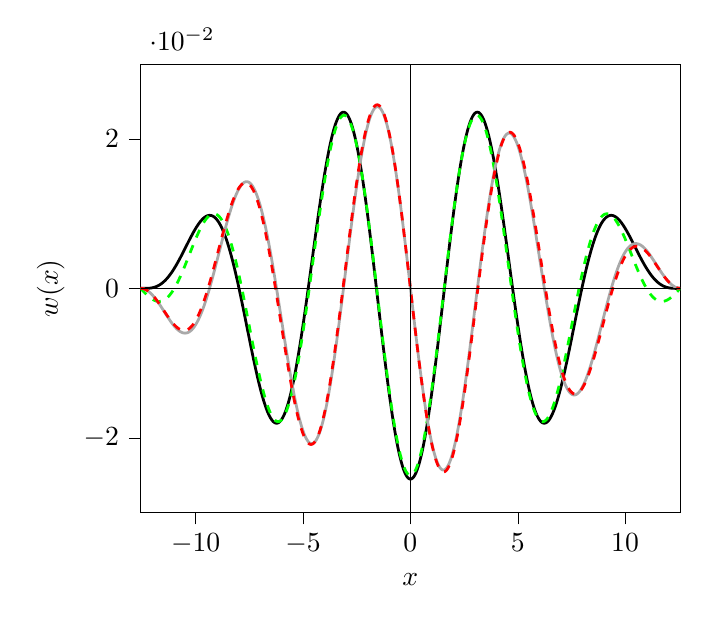
\begin{tikzpicture}

\definecolor{darkgray}{RGB}{169,169,169}
\definecolor{darkgray176}{RGB}{176,176,176}

\begin{axis}[
tick align=outside,
tick pos=left,
x grid style={darkgray176},
xlabel={\(\displaystyle x\)},
xmin=-12.5663706143592, xmax=12.5663706143592,
xtick style={color=black},
y grid style={darkgray176},
ylabel={\(\displaystyle w(x)\)},
ymin=-0.03, ymax=0.03,
ytick style={color=black}
]
\addplot [line width=1pt, black]
table {%
-12.5663706143592 0
-12.5463706143592 -1.18049301471451e-07
-12.5263706143592 -4.37966505707027e-07
-12.5063706143592 -9.0828694165573e-07
-12.4863706143592 -1.47742173070005e-06
-12.4663706143592 -2.0937002910945e-06
-12.4463706143592 -2.70541289398071e-06
-12.4263706143592 -3.26085324413985e-06
-12.4063706143592 -3.70836105849396e-06
-12.3863706143592 -3.99636461600522e-06
-12.3663706143592 -4.07342325142552e-06
-12.3463706143592 -3.88826976643384e-06
-12.3263706143592 -3.38985273148858e-06
-12.3063706143592 -2.52737865150997e-06
-12.2863706143592 -1.25035396861776e-06
-12.2663706143592 4.91373124247887e-07
-12.2463706143592 2.74757108541751e-06
-12.2263706143592 5.56758366892641e-06
-12.2063706143592 9.00028883685626e-06
-12.1863706143592 1.30940579661e-05
-12.1663706143592 1.78967153751e-05
-12.1463706143592 2.34554981965e-05
-12.1263706143592 2.9817016621e-05
-12.1063706143592 3.70272145374e-05
-12.0863706143592 4.51313305945e-05
-12.0663706143592 5.41738597095e-05
-12.0463706143592 6.41985150463e-05
-12.0263706143592 7.52481904902e-05
-12.0063706143592 8.73649236403e-05
-11.9863706143592 0.0001005898593461
-11.9663706143592 0.0001149632138088
-11.9463706143592 0.0001305242392729
-11.9263706143592 0.0001473111893289
-11.9063706143592 0.0001653612848509
-11.8863706143592 0.0001847106805899
-11.8663706143592 0.000205394432445
-11.8463706143592 0.0002274464654343
-11.8263706143592 0.0002508995423848
-11.8063706143592 0.0002757852333631
-11.7863706143592 0.0003021338858666
-11.7663706143592 0.0003299745957942
-11.7463706143592 0.000359335179216
-11.7263706143592 0.0003902421449611
-11.7063706143592 0.00042272066804
-11.6863706143592 0.0004567945639222
-11.6663706143592 0.0004924862636829
-11.6463706143592 0.0005298167900381
-11.6263706143592 0.0005688057342828
-11.6063706143592 0.0006094712341484
-11.5863706143592 0.0006518299525952
-11.5663706143592 0.0006958970575526
-11.5463706143592 0.0007416862026239
-11.5263706143592 0.0007892095087662
-11.5063706143592 0.0008384775469607
-11.4863706143592 0.0008894993218849
-11.4663706143592 0.0009422822565975
-11.4463706143592 0.0009968321782491
-11.4263706143592 0.0010531533048281
-11.4063706143592 0.0011112482329517
-11.3863706143592 0.0011711179267121
-11.3663706143592 0.001232761707586
-11.3463706143592 0.0012961772454168
-11.3263706143592 0.0013613605504745
-11.3063706143592 0.0014283059666039
-11.2863706143592 0.0014970061654635
-11.2663706143592 0.0015674521418642
-11.2463706143592 0.0016396332102102
-11.2263706143592 0.0017135370020481
-11.2063706143592 0.001789149464727
-11.1863706143592 0.0018664548611735
-11.1663706143592 0.0019454357707833
-11.1463706143592 0.0020260730914314
-11.1263706143592 0.0021083460426022
-11.1063706143592 0.0021922321696402
-11.0863706143592 0.0022777073491202
-11.0663706143592 0.0023647457953373
-11.0463706143592 0.0024533200679141
-11.0263706143592 0.0025434010805241
-11.0063706143592 0.0026349581107274
-10.9863706143592 0.0027279588109161
-10.9663706143592 0.0028223692203646
-10.9463706143592 0.0029181537783805
-10.9263706143592 0.0030152753385506
-10.9063706143592 0.0031136951840754
-10.8863706143592 0.0032133730441868
-10.8663706143592 0.0033142671116393
-10.8463706143592 0.0034163340612696
-10.8263706143592 0.0035195290696131
-10.8063706143592 0.00362380583557
-10.7863706143592 0.0037291166021112
-10.7663706143592 0.0038354121790112
-10.7463706143592 0.0039426419665999
-10.7263706143592 0.0040507539805195
-10.7063706143592 0.004159694877475
-10.6863706143592 0.004269409981965
-10.6663706143592 0.0043798433139796
-10.6463706143592 0.0044909376176512
-10.6263706143592 0.004602634390843
-10.6063706143592 0.0047148739156611
-10.5863706143592 0.0048275952898729
-10.5663706143592 0.0049407364592167
-10.5463706143592 0.005054234250585
-10.5263706143592 0.0051680244060637
-10.5063706143592 0.00528204161781
-10.4863706143592 0.00539621956375
-10.4663706143592 0.0055104909440771
-10.4463706143592 0.0056247875185315
-10.4263706143592 0.0057390401444412
-10.4063706143592 0.0058531788155035
-10.3863706143592 0.0059671327012869
-10.3663706143592 0.0060808301874308
-10.3463706143592 0.0061941989165219
-10.3263706143592 0.0063071658296255
-10.3063706143592 0.0064196572084475
-10.2863706143592 0.0065315987181057
-10.2663706143592 0.0066429154504858
-10.2463706143592 0.0067535319681579
-10.2263706143592 0.0068633723488312
-10.2063706143592 0.0069723602303197
-10.1863706143592 0.0070804188559952
-10.1663706143592 0.0071874711207034
-10.1463706143592 0.0072934396171148
-10.1263706143592 0.0073982466824871
-10.1063706143592 0.0075018144458115
-10.0863706143592 0.0076040648753165
-10.0663706143592 0.0077049198263028
-10.0463706143592 0.0078043010892824
-10.0263706143592 0.0079021304383938
-10.0063706143592 0.0079983296800674
-9.98637061435917 0.0080928207019119
-9.96637061435917 0.0081855255217943
-9.94637061435917 0.0082763663370865
-9.92637061435917 0.0083652655740488
-9.90637061435917 0.0084521459373228
-9.88637061435917 0.0085369304595058
-9.86637061435917 0.0086195425507765
-9.84637061435917 0.0086999060485452
-9.82637061435917 0.0087779452670986
-9.80637061435917 0.0088535850472108
-9.78637061435917 0.0089267508056913
-9.76637061435917 0.0089973685848424
-9.74637061435917 0.0090653651017948
-9.72637061435917 0.0091306677976951
-9.70637061435917 0.0091932048867144
-9.68637061435917 0.0092529054048499
-9.66637061435917 0.009309699258491
-9.64637061435917 0.0093635172727206
-9.62637061435917 0.009414291239323
-9.60637061435917 0.0094619539644705
-9.58637061435917 0.0095064393160591
-9.56637061435917 0.0095476822706667
-9.54637061435917 0.0095856189601032
-9.52637061435917 0.0096201867175272
-9.50637061435917 0.0096513241230989
-9.48637061435917 0.009678971049144
-9.46637061435917 0.009703068704799
-9.44637061435917 0.0097235596801115
-9.42637061435917 0.0097403879895698
-9.40637061435917 0.0097534991150321
-9.38637061435917 0.009762840048032
-9.36637061435917 0.0097683593314322
-9.34637061435917 0.0097700071004005
-9.32637061435917 0.0097677351226837
-9.30637061435917 0.0097614968381533
-9.28637061435917 0.0097512473975977
-9.26637061435917 0.0097369437007374
-9.24637061435917 0.0097185444334381
-9.22637061435917 0.0096960101040984
-9.20637061435917 0.0096693030791887
-9.18637061435917 0.0096383876179171
-9.16637061435917 0.0096032299060022
-9.14637061435917 0.0095637980885278
-9.12637061435917 0.0095200623018599
-9.10637061435917 0.0094719947046035
-9.08637061435917 0.0094195695075794
-9.06637061435917 0.0093627630027997
-9.04637061435917 0.0093015535914234
-9.02637061435917 0.009235921810671
-9.00637061435917 0.0091658503596819
-8.98637061435917 0.0090913241242941
-8.96637061435917 0.0090123302007291
-8.94637061435917 0.0089288579181662
-8.92637061435917 0.0088408988601877
-8.90637061435917 0.0087484468850802
-8.88637061435917 0.0086514981449761
-8.86637061435917 0.0085500511038208
-8.84637061435917 0.0084441065541517
-8.82637061435917 0.0083336676326737
-8.80637061435917 0.0082187398346209
-8.78637061435917 0.0080993310268897
-8.76637061435917 0.0079754514599331
-8.74637061435917 0.0078471137784041
-8.72637061435917 0.0077143330305393
-8.70637061435917 0.0075771266762704
-8.68637061435917 0.0074355145940576
-8.66637061435917 0.0072895190864336
-8.64637061435917 0.0071391648842527
-8.62637061435917 0.0069844791496361
-8.60637061435917 0.0068254914776087
-8.58637061435917 0.00666223389642
-8.56637061435917 0.0064947408665458
-8.54637061435917 0.006323049278365
-8.52637061435917 0.0061471984485085
-8.50637061435917 0.0059672301148778
-8.48637061435917 0.0057831884303299
-8.46637061435917 0.0055951199550283
-8.44637061435917 0.0054030736474583
-8.42637061435917 0.0052071008541077
-8.40637061435917 0.005007255297812
-8.38637061435917 0.0048035930647676
-8.36637061435917 0.004596172590213
-8.34637061435917 0.004385054642782
-8.32637061435917 0.0041703023075329
-8.30637061435917 0.0039519809676567
-8.28637061435917 0.0037301582848701
-8.26637061435917 0.0035049041784989
-8.24637061435917 0.0032762908032586
-8.22637061435917 0.0030443925257384
-8.20637061435917 0.0028092858995973
-8.18637061435917 0.0025710496394809
-8.16637061435917 0.0023297645936672
-8.14637061435917 0.002085513715453
-8.12637061435917 0.0018383820332899
-8.10637061435917 0.0015884566196821
-8.08637061435917 0.001335826558859
-8.06637061435917 0.0010805829132326
-8.04637061435917 0.0008228186886568
-8.02637061435917 0.000562628798499
-8.00637061435917 0.0003001100265422
-7.98637061435917 3.53609887304e-05
-7.96637061435917 -0.0002315179062253
-7.94637061435917 -0.0005004244973639
-7.92637061435917 -0.0007712549130963
-7.90637061435917 -0.0010439036139152
-7.88637061435917 -0.0013182634361739
-7.86637061435917 -0.0015942256369144
-7.84637061435917 -0.0018716799397253
-7.82637061435917 -0.0021505145816094
-7.80637061435917 -0.0024306163608389
-7.78637061435917 -0.0027118706857776
-7.76637061435917 -0.0029941616246476
-7.74637061435917 -0.0032773719562179
-7.72637061435917 -0.0035613832213906
-7.70637061435917 -0.0038460757756627
-7.68637061435917 -0.0041313288424372
-7.66637061435917 -0.0044170205671608
-7.64637061435917 -0.0047030280722604
-7.62637061435917 -0.0049892275128544
-7.60637061435917 -0.0052754941332118
-7.58637061435917 -0.0055617023239323
-7.56637061435917 -0.0058477256798204
-7.54637061435917 -0.0061334370584256
-7.52637061435917 -0.0064187086392201
-7.50637061435917 -0.0067034119833874
-7.48637061435917 -0.0069874180941901
-7.46637061435917 -0.0072705974778902
-7.44637061435917 -0.0075528202051902
-7.42637061435917 -0.0078339559731674
-7.40637061435917 -0.0081138741676678
-7.38637061435917 -0.0083924439261321
-7.36637061435917 -0.0086695342008212
-7.34637061435917 -0.00894501382241
-7.32637061435917 -0.0092187515639187
-7.30637061435917 -0.0094906162049488
-7.28637061435917 -0.0097604765961931
-7.26637061435917 -0.0100282017241857
-7.24637061435917 -0.0102936607762618
-7.22637061435917 -0.0105567232056921
-7.20637061435917 -0.0108172587969613
-7.18637061435917 -0.0110751377311559
-7.16637061435917 -0.0113302306514293
-7.14637061435917 -0.0115824087285109
-7.12637061435917 -0.0118315437262243
-7.10637061435917 -0.012077508066984
-7.08637061435917 -0.0123201748972338
-7.06637061435917 -0.012559418152796
-7.04637061435917 -0.012795112624096
-7.02637061435917 -0.0130271340212296
-7.00637061435917 -0.013255359038839
-6.98637061435917 -0.0134796654207634
-6.96637061435917 -0.0136999320244319
-6.94637061435917 -0.0139160388849629
-6.92637061435917 -0.0141278672789395
-6.90637061435917 -0.014335299787824
-6.88637061435917 -0.0145382203609813
-6.86637061435917 -0.0147365143782756
-6.84637061435917 -0.0149300687122091
-6.82637061435917 -0.015118771789568
-6.80637061435917 -0.0153025136525451
-6.78637061435917 -0.0154811860193039
-6.76637061435917 -0.0156546823439544
-6.74637061435917 -0.0158228978759065
-6.72637061435917 -0.0159857297185698
-6.70637061435917 -0.016143076887368
-6.68637061435917 -0.0162948403670369
-6.66637061435917 -0.0164409231681741
-6.64637061435917 -0.0165812303830102
-6.62637061435917 -0.0167156692403703
-6.60637061435917 -0.0168441491597968
-6.58637061435917 -0.0169665818048022
-6.56637061435917 -0.0170828811352235
-6.54637061435917 -0.0171929634586493
-6.52637061435917 -0.0172967474808892
-6.50637061435917 -0.0173941543554593
-6.48637061435917 -0.0174851077320554
-6.46637061435917 -0.0175695338039853
-6.44637061435917 -0.0176473613545349
-6.42637061435917 -0.0177185218022405
-6.40637061435917 -0.017782949245042
-6.38637061435917 -0.0178405805032915
-6.36637061435917 -0.0178913551615911
-6.34637061435917 -0.0179352156094381
-6.32637061435917 -0.0179721070806506
-6.30637061435917 -0.0180019776915526
-6.28637061435917 -0.0180247784778949
-6.26637061435917 -0.0180404634304889
-6.24637061435917 -0.0180489895295337
-6.22637061435917 -0.0180503167776133
-6.20637061435917 -0.0180444082313449
-6.18637061435917 -0.0180312300316586
-6.16637061435917 -0.0180107514326885
-6.14637061435917 -0.0179829448292577
-6.12637061435917 -0.017947785782939
-6.10637061435917 -0.0179052530466742
-6.08637061435917 -0.0178553285879356
-6.06637061435917 -0.0177979976104146
-6.04637061435917 -0.0177332485742209
-6.02637061435917 -0.0176610732145795
-6.00637061435917 -0.0175814665590118
-5.98637061435917 -0.0174944269429862
-5.96637061435917 -0.0173999560240289
-5.94637061435917 -0.0172980587942806
-5.92637061435917 -0.0171887435914907
-5.90637061435917 -0.0170720221084383
-5.88637061435917 -0.0169479094007702
-5.86637061435917 -0.0168164238932489
-5.84637061435917 -0.0166775873844022
-5.82637061435917 -0.0165314250495675
-5.80637061435917 -0.0163779654423256
-5.78637061435917 -0.0162172404943174
-5.76637061435917 -0.0160492855134413
-5.74637061435917 -0.0158741391804248
-5.72637061435917 -0.0156918435437703
-5.70637061435917 -0.0155024440130711
-5.68637061435917 -0.0153059893506971
-5.66637061435917 -0.0151025316618501
-5.64637061435917 -0.0148921263829885
-5.62637061435917 -0.0146748322686233
-5.60637061435917 -0.0144507113764863
-5.58637061435917 -0.014219829051075
-5.56637061435917 -0.0139822539055763
-5.54637061435917 -0.013738057802174
-5.52637061435917 -0.0134873158307463
-5.50637061435917 -0.0132301062859575
-5.48637061435917 -0.0129665106427528
-5.46637061435917 -0.0126966135302619
-5.44637061435917 -0.0124205027041222
-5.42637061435917 -0.0121382690172287
-5.40637061435917 -0.0118500063889218
-5.38637061435917 -0.0115558117726243
-5.36637061435917 -0.0112557851219383
-5.34637061435917 -0.0109500293552147
-5.32637061435917 -0.0106386503186094
-5.30637061435917 -0.0103217567476391
-5.28637061435917 -0.009999460227252
-5.26637061435917 -0.0096718751504294
-5.24637061435917 -0.0093391186753333
-5.22637061435917 -0.0090013106810188
-5.20637061435917 -0.0086585737217269
-5.18637061435917 -0.0083110329797791
-5.16637061435917 -0.0079588162170898
-5.14637061435917 -0.0076020537253191
-5.12637061435917 -0.0072408782746857
-5.10637061435917 -0.0068754250614612
-5.08637061435917 -0.0065058316541678
-5.06637061435917 -0.0061322379385029
-5.04637061435917 -0.0057547860610132
-5.02637061435917 -0.0053736203715432
-5.00637061435917 -0.0049888873644819
-4.98637061435917 -0.004600735618834
-4.96637061435917 -0.0042093157371409
-4.94637061435917 -0.0038147802832796
-4.92637061435917 -0.0034172837191637
-4.90637061435917 -0.0030169823403783
-4.88637061435917 -0.002614034210774
-4.86637061435917 -0.0022085990960504
-4.84637061435917 -0.0018008383963586
-4.82637061435917 -0.0013909150779524
-4.80637061435917 -0.0009789936039193
-4.78637061435917 -0.0005652398640213
-4.76637061435917 -0.0001498211036789
-4.74637061435917 0.0002670941478716
-4.72637061435917 0.0006853361502138
-4.70637061435917 0.0011047340251462
-4.68637061435917 0.0015251158308058
-4.66637061435917 0.0019463086364829
-4.64637061435917 0.0023681385980959
-4.62637061435917 0.0027904310342898
-4.60637061435917 0.0032130105031232
-4.58637061435917 0.0036357008793103
-4.56637061435917 0.0040583254319799
-4.54637061435917 0.0044807069029171
-4.52637061435917 0.0049026675852505
-4.50637061435917 0.0053240294025486
-4.48637061435917 0.005744613988289
-4.46637061435917 0.0061642427656619
-4.44637061435917 0.0065827370276727
-4.42637061435917 0.0069999180175036
-4.40637061435917 0.0074156070090993
-4.38637061435917 0.0078296253879365
-4.36637061435917 0.0082417947319398
-4.34637061435917 0.0086519368925072
-4.32637061435917 0.0090598740756045
-4.30637061435917 0.0094654289228919
-4.28637061435917 0.009868424592844
-4.26637061435917 0.0102686848418241
-4.24637061435917 0.0106660341050741
-4.22637061435917 0.0110602975775826
-4.20637061435917 0.0114513012947909
-4.18637061435917 0.0118388722130994
-4.16637061435917 0.0122228382901353
-4.14637061435917 0.0126030285647427
-4.12637061435917 0.0129792732366583
-4.10637061435917 0.0133514037458314
-4.08637061435917 0.0137192528513525
-4.06637061435917 0.0140826547099513
-4.04637061435917 0.014441444954026
-4.02637061435917 0.014795460769166
-4.00637061435917 0.0151445409711304
-3.98637061435917 0.0154885260822455
-3.96637061435917 0.0158272584071826
-3.94637061435917 0.0161605821080803
-3.92637061435917 0.016488343278974
-3.90637061435917 0.0168103900194965
-3.88637061435917 0.0171265725078124
-3.86637061435917 0.0174367430727523
-3.84637061435917 0.0177407562651093
-3.82637061435917 0.0180384689280634
-3.80637061435917 0.0183297402666998
-3.78637061435917 0.0186144319165848
-3.76637061435917 0.0188924080113668
-3.74637061435917 0.0191635352493679
-3.72637061435917 0.0194276829591332
-3.70637061435917 0.019684723163905
-3.68637061435917 0.0199345306449894
-3.66637061435917 0.020176983003984
-3.64637061435917 0.0204119607238342
-3.62637061435917 0.020639347228689
-3.60637061435917 0.0208590289425246
-3.58637061435917 0.0210708953465063
-3.56637061435917 0.0212748390350607
-3.54637061435917 0.0214707557706274
-3.52637061435917 0.021658544537065
-3.50637061435917 0.0218381075916809
-3.48637061435917 0.022009350515861
-3.46637061435917 0.0221721822642711
-3.44637061435917 0.0223265152126056
-3.42637061435917 0.0224722652038578
-3.40637061435917 0.0226093515930891
-3.38637061435917 0.0227376972906716
-3.36637061435917 0.0228572288039828
-3.34637061435917 0.02296787627753
-3.32637061435917 0.023069573531483
-3.30637061435917 0.0231622580985937
-3.28637061435917 0.0232458712594842
-3.26637061435917 0.0233203580762831
-3.24637061435917 0.023385667424592
-3.22637061435917 0.0234417520237648
-3.20637061435917 0.0234885684654825
-3.18637061435917 0.023526077240608
-3.16637061435917 0.0235542427643057
-3.14637061435917 0.0235730333994102
-3.12637061435917 0.0235824214780334
-3.10637061435917 0.0235823833213932
-3.08637061435917 0.0235728992578559
-3.06637061435917 0.023553953639178
-3.04637061435917 0.0235255348549397
-3.02637061435917 0.0234876353451582
-3.00637061435917 0.0234402516110743
-2.98637061435917 0.0233833842241039
-2.96637061435917 0.023317037832947
-2.94637061435917 0.023241221168849
-2.92637061435917 0.0231559470490091
-2.90637061435917 0.0230612323781311
-2.88637061435917 0.0229570981481139
-2.86637061435917 0.0228435694358787
-2.84637061435917 0.022720675399332
-2.82637061435917 0.0225884492714628
-2.80637061435917 0.022446928352575
-2.78637061435917 0.0222961540006561
-2.76637061435917 0.022136171619883
-2.74637061435917 0.0219670306472701
-2.72637061435917 0.0217887845374602
-2.70637061435917 0.0216014907456667
-2.68637061435917 0.0214052107087684
-2.66637061435917 0.0212000098245678
-2.64637061435917 0.0209859574292158
-2.62637061435917 0.0207631267728147
-2.60637061435917 0.0205315949932058
-2.58637061435917 0.0202914430879533
-2.56637061435917 0.020042755884534
-2.54637061435917 0.0197856220087461
-2.52637061435917 0.0195201338513469
-2.50637061435917 0.0192463875329363
-2.48637061435917 0.018964482867097
-2.46637061435917 0.0186745233218083
-2.44637061435917 0.0183766159791493
-2.42637061435917 0.0180708714933073
-2.40637061435917 0.0177574040469099
-2.38637061435917 0.017436331305698
-2.36637061435917 0.017107774371561
-2.34637061435917 0.0167718577339509
-2.32637061435917 0.0164287092196989
-2.30637061435917 0.016078459941255
-2.28637061435917 0.0157212442433721
-2.26637061435917 0.0153571996482589
-2.24637061435917 0.0149864667992245
-2.22637061435917 0.0146091894028397
-2.20637061435917 0.0142255141696398
-2.18637061435917 0.0138355907533953
-2.16637061435917 0.0134395716889769
-2.14637061435917 0.013037612328842
-2.12637061435917 0.0126298707781712
-2.10637061435917 0.0122165078286831
-2.08637061435917 0.0117976868911565
-2.06637061435917 0.0113735739266908
-2.04637061435917 0.0109443373767342
-2.02637061435917 0.0105101480919117
-2.00637061435917 0.0100711792596844
-1.98637061435917 0.0096276063308719
-1.96637061435917 0.0091796069450719
-1.94637061435917 0.0087273608550099
-1.92637061435917 0.0082710498498522
-1.90637061435917 0.0078108576775186
-1.88637061435917 0.0073469699660277
-1.86637061435917 0.0068795741439122
-1.84637061435917 0.0064088593597391
-1.82637061435917 0.005935016400771
-1.80637061435917 0.005458237610807
-1.78637061435917 0.0049787168072382
-1.76637061435917 0.0044966491973572
-1.74637061435917 0.0040122312939594
-1.72637061435917 0.0035256608302735
-1.70637061435917 0.0030371366742612
-1.68637061435917 0.0025468587423249
-1.66637061435917 0.0020550279124623
-1.64637061435917 0.0015618459369077
-1.62637061435917 0.0010675153543008
-1.60637061435917 0.0005722394014219
-1.58637061435917 7.62219245357e-05
-1.56637061435917 -0.000420332709618
-1.54637061435917 -0.000917219703144
-1.52637061435917 -0.0014142339165809
-1.50637061435917 -0.0019111699587193
-1.48637061435917 -0.0024078222766078
-1.46637061435917 -0.0029039852457047
-1.44637061435917 -0.0033994532601342
-1.42637061435917 -0.0038940208230053
-1.40637061435917 -0.0043874826367523
-1.38637061435917 -0.0048796336934547
-1.36637061435917 -0.0053702693650949
-1.34637061435917 -0.0058591854937119
-1.32637061435917 -0.0063461784814097
-1.30637061435917 -0.0068310453801787
-1.28637061435917 -0.0073135839814879
-1.26637061435917 -0.0077935929056075
-1.24637061435917 -0.008270871690619
-1.22637061435917 -0.0087452208810742
-1.20637061435917 -0.009216442116258
-1.18637061435917 -0.0096843382180186
-1.16637061435917 -0.0101487132781202
-1.14637061435917 -0.0106093727450809
-1.12637061435917 -0.0110661235104537
-1.10637061435917 -0.0115187739945104
-1.08637061435917 -0.0119671342312898
-1.06637061435917 -0.0124110159529696
-1.04637061435917 -0.0128502326735232
-1.02637061435917 -0.0132845997716227
-1.00637061435917 -0.0137139345727482
-0.986370614359172 -0.0141380564304674
-0.966370614359173 -0.0145567868068456
-0.946370614359172 -0.0149699493519498
-0.926370614359172 -0.0153773699824091
-0.906370614359172 -0.0157788769589957
-0.886370614359173 -0.0161743009631893
-0.866370614359171 -0.0165634751726899
-0.846370614359172 -0.0169462353358432
-0.826370614359172 -0.017322419844945
-0.806370614359173 -0.0176918698083883
-0.786370614359173 -0.0180544291216218
-0.766370614359172 -0.018409944536885
-0.746370614359172 -0.0187582657316876
-0.726370614359173 -0.0190992453760022
-0.706370614359173 -0.0194327391981371
-0.686370614359172 -0.0197586060492606
-0.666370614359172 -0.0200767079665444
-0.646370614359173 -0.0203869102348981
-0.626370614359173 -0.0206890814472655
-0.606370614359172 -0.0209830935634544
-0.586370614359172 -0.0212688219674721
-0.566370614359172 -0.0215461455233402
-0.546370614359173 -0.0218149466293629
-0.526370614359172 -0.0220751112708222
-0.506370614359172 -0.0223265290710761
-0.486370614359172 -0.0225690933410366
-0.466370614359173 -0.0228027011270025
-0.446370614359171 -0.0230272532568263
-0.426370614359172 -0.0232426543843927
-0.406370614359172 -0.0234488130323876
-0.386370614359173 -0.023645641633339
-0.366370614359171 -0.0238330565689083
-0.346370614359172 -0.0240109782074159
-0.326370614359172 -0.0241793309395819
-0.306370614359173 -0.0243380432124656
-0.286370614359171 -0.0244870475615883
-0.266370614359172 -0.024626280641224
-0.246370614359172 -0.0247556832528433
-0.226370614359173 -0.0248752003716981
-0.206370614359173 -0.0249847811715342
-0.186370614359172 -0.0250843790474198
-0.166370614359172 -0.0251739516366801
-0.146370614359173 -0.025253460837927
-0.126370614359173 -0.0253228728281765
-0.106370614359172 -0.0253821580780437
-0.086370614359172 -0.0254312913650109
-0.0663706143591724 -0.0254702517847597
-0.0463706143591728 -0.0254990227605643
-0.0263706143591715 -0.02551759205074
-0.0063706143591719 -0.0255259517541439
0.0136293856408276 -0.0255240983137254
0.0336293856408271 -0.0255120325181248
0.0536293856408285 -0.0254897595013185
0.0736293856408281 -0.0254572887403124
0.0936293856408276 -0.0254146340508832
0.113629385640827 -0.02536181358137
0.133629385640829 -0.0252988498045203
0.153629385640828 -0.0252257695073919
0.173629385640828 -0.0251426037793175
0.193629385640827 -0.0250493879979369
0.213629385640829 -0.0249461618133028
0.233629385640828 -0.024832969130069
0.253629385640828 -0.0247098580877678
0.273629385640827 -0.0245768810391871
0.293629385640827 -0.0244340945268568
0.313629385640828 -0.024281559257655
0.333629385640828 -0.0241193400755478
0.353629385640827 -0.0239475059324725
0.373629385640827 -0.0237661298573812
0.393629385640828 -0.0235752889234564
0.413629385640828 -0.023375064213516
0.433629385640827 -0.0231655407836226
0.453629385640827 -0.0229468076249156
0.473629385640828 -0.0227189576236817
0.493629385640828 -0.0224820875196858
0.513629385640828 -0.0222362978627781
0.533629385640827 -0.0219816929678009
0.553629385640829 -0.0217183808678144
0.573629385640828 -0.0214464732656643
0.593629385640828 -0.0211660854839131
0.613629385640827 -0.0208773364131589
0.633629385640829 -0.0205803484587671
0.653629385640828 -0.0202752474860376
0.673629385640828 -0.0199621627638348
0.693629385640827 -0.0196412269067068
0.713629385640829 -0.0193125758155201
0.733629385640828 -0.0189763486166383
0.753629385640828 -0.0186326875996722
0.773629385640827 -0.0182817381538325
0.793629385640827 -0.0179236487029121
0.813629385640828 -0.0175585706389308
0.833629385640828 -0.0171866582544723
0.853629385640827 -0.0168080686737444
0.873629385640827 -0.0164229617823971
0.893629385640828 -0.0160315001561283
0.913629385640828 -0.0156338489881129
0.933629385640828 -0.0152301760152874
0.953629385640827 -0.0148206514435261
0.973629385640828 -0.0144054478717422
0.993629385640828 -0.0139847402149506
1.01362938564083 -0.0135587056263269
1.03362938564083 -0.0131275234183006
1.05362938564083 -0.0126913749827176
1.07362938564083 -0.0122504437101104
1.09362938564083 -0.0118049149081129
1.11362938564083 -0.0113549757190588
1.13362938564083 -0.0109008150368
1.15362938564083 -0.0104426234227863
1.17362938564083 -0.0099805930214436
1.19362938564083 -0.0095149174748896
1.21362938564083 -0.0090457918370294
1.23362938564083 -0.0085734124870672
1.25362938564083 -0.0080979770424772
1.27362938564083 -0.0076196842714727
1.29362938564083 -0.0071387340050145
1.31362938564083 -0.0066553270483988
1.33362938564083 -0.0061696650924671
1.35362938564083 -0.005681950624477
1.37362938564083 -0.0051923868386773
1.39362938564083 -0.0047011775466279
1.41362938564083 -0.0042085270873057
1.43362938564083 -0.0037146402370384
1.45362938564083 -0.0032197221193085
1.47362938564083 -0.0027239781144682
1.49362938564083 -0.0022276137694069
1.51362938564083 -0.0017308347072143
1.53362938564083 -0.0012338465368788
1.55362938564083 -0.0007368547630646
1.57362938564083 -0.0002400646960086
1.59362938564083 0.0002563186384228
1.61362938564083 0.0007520905884735
1.63362938564083 0.0012470469659937
1.65362938564083 0.0017409841356518
1.67362938564083 0.0022336991038197
1.69362938564083 0.0027249896070926
1.71362938564083 0.0032146542004004
1.73362938564083 0.0037024923446723
1.75362938564083 0.0041883044940136
1.77362938564083 0.0046718921823553
1.79362938564083 0.0051530581095357
1.81362938564083 0.0056316062267765
1.83362938564083 0.0061073418215132
1.85362938564083 0.0065800716015413
1.87362938564083 0.0070496037784402
1.89362938564083 0.0075157481502373
1.91362938564083 0.0079783161832734
1.93362938564083 0.008437121093234
1.95362938564083 0.0088919779253082
1.97362938564083 0.0093427036334406
1.99362938564083 0.0097891171586384
2.01362938564083 0.0102310395062997
2.03362938564083 0.0106682938225286
2.05362938564083 0.0111007054694006
2.07362938564083 0.0115281020991473
2.09362938564083 0.0119503137272243
2.11362938564083 0.0123671728042321
2.13362938564083 0.0127785142866557
2.15362938564083 0.0131841757063931
2.17362938564083 0.0135839972390404
2.19362938564083 0.0139778217709036
2.21362938564083 0.0143654949647079
2.23362938564083 0.014746865323974
2.25362938564083 0.015121784256035
2.27362938564083 0.0154901061336641
2.29362938564083 0.0158516883552873
2.31362938564083 0.016206391403754
2.33362938564083 0.0165540789036401
2.35362938564083 0.0168946176770596
2.37362938564083 0.0172278777979576
2.39362938564083 0.017553732644865
2.41362938564083 0.0178720589520888
2.43362938564083 0.0181827368593183
2.45362938564083 0.0184856499596248
2.47362938564083 0.0187806853458345
2.49362938564083 0.0190677336552551
2.51362938564083 0.019346689112738
2.53362938564083 0.0196174495720559
2.55362938564083 0.0198799165555819
2.57362938564083 0.0201339952922496
2.59362938564083 0.0203795947537827
2.61362938564083 0.0206166276891761
2.63362938564083 0.0208450106574171
2.65362938564083 0.0210646640584315
2.67362938564083 0.0212755121622442
2.69362938564083 0.0214774831363414
2.71362938564083 0.0216705090712258
2.73362938564083 0.0218545260041533
2.75362938564083 0.0220294739410431
2.77362938564083 0.0221952968765548
2.79362938564083 0.0223519428123227
2.81362938564083 0.022499363773344
2.83362938564083 0.0226375158225136
2.85362938564083 0.0227663590733031
2.87362938564083 0.0228858577005783
2.89362938564083 0.0229959799495548
2.91362938564083 0.0230966981428886
2.93362938564083 0.0231879886859018
2.95362938564083 0.023269832069943
2.97362938564083 0.0233422128738835
2.99362938564083 0.0234051197637512
3.01362938564083 0.0234585454905052
3.03362938564083 0.0235024868859546
3.05362938564083 0.0235369448568259
3.07362938564083 0.0235619243769842
3.09362938564083 0.0235774344778152
3.11362938564083 0.0235834882367748
3.13362938564083 0.0235801027641136
3.15362938564083 0.0235672991877865
3.17362938564083 0.0235451026365559
3.19362938564083 0.0235135422212997
3.21362938564083 0.0234726510145358
3.23362938564083 0.023422466028174
3.25362938564083 0.0233630281895103
3.27362938564083 0.0232943823154759
3.29362938564083 0.0232165770851561
3.31362938564083 0.0231296650105953
3.33362938564083 0.0230337024059029
3.35362938564083 0.0229287493546793
3.37362938564083 0.0228148696757774
3.39362938564083 0.0226921308874205
3.41362938564083 0.0225606041696947
3.43362938564083 0.0224203643254359
3.45362938564083 0.0222714897395334
3.47362938564083 0.0221140623366708
3.49362938564083 0.021948167537526
3.51362938564083 0.0217738942134552
3.53362938564083 0.021591334639683
3.55362938564083 0.0214005844470234
3.57362938564083 0.0212017425721569
3.59362938564083 0.0209949112064901
3.61362938564083 0.0207801957436229
3.63362938564083 0.0205577047254507
3.65362938564083 0.020327549786931
3.67362938564083 0.0200898455995387
3.69362938564083 0.0198447098134438
3.71362938564083 0.0195922629984366
3.73362938564083 0.0193326285836328
3.75362938564083 0.0190659327959884
3.77362938564083 0.0187923045976552
3.79362938564083 0.0185118756222082
3.81362938564083 0.0182247801097777
3.83362938564083 0.0179311548411179
3.85362938564083 0.0176311390706449
3.87362938564083 0.0173248744584781
3.89362938564083 0.0170125050015182
3.91362938564083 0.0166941769635961
3.93362938564083 0.016370038804728
3.95362938564083 0.0160402411095106
3.97362938564083 0.0157049365146926
3.99362938564083 0.0153642796359577
4.01362938564083 0.0150184269939555
4.03362938564083 0.0146675369396166
4.05362938564083 0.0143117695787875
4.07362938564083 0.0139512866962237
4.09362938564083 0.0135862516789777
4.11362938564083 0.0132168294392178
4.13362938564083 0.0128431863365176
4.15362938564083 0.0124654900996521
4.17362938564083 0.0120839097479391
4.19362938564083 0.0116986155121644
4.21362938564083 0.0113097787551271
4.23362938564083 0.010917571891847
4.25362938564083 0.0105221683094681
4.27362938564083 0.0101237422869001
4.29362938564083 0.0097224689142354
4.31362938564083 0.0093185240119794
4.33362938564083 0.008912084050134
4.35362938564083 0.0085033260671724
4.37362938564083 0.008092427588944
4.39362938564083 0.0076795665475473
4.41362938564083 0.0072649212002106
4.43362938564083 0.0068486700482182
4.45362938564083 0.0064309917559203
4.47362938564083 0.0060120650698658
4.49362938564083 0.005592068738095
4.51362938564083 0.0051711814296309
4.53362938564083 0.0047495816542077
4.55362938564083 0.0043274476822715
4.57362938564083 0.0039049574652947
4.59362938564083 0.0034822885564373
4.61362938564083 0.003059618031595
4.63362938564083 0.0026371224108695
4.65362938564083 0.0022149775804976
4.67362938564083 0.0017933587152759
4.69362938564083 0.0013724402015161
4.71362938564083 0.0009523955605673
4.73362938564083 0.0005333973729402
4.75362938564083 0.0001156172030675
4.77362938564083 -0.0003007744752636
4.79362938564083 -0.000715608352775
4.81362938564083 -0.0011287163578203
4.83362938564083 -0.0015399317287371
4.85362938564083 -0.0019490890853928
4.87362938564083 -0.0023560244998938
4.89362938564083 -0.0027605755664251
4.91362938564083 -0.0031625814701887
4.93362938564083 -0.0035618830554108
4.95362938564083 -0.0039583228923871
4.97362938564083 -0.0043517453435349
4.99362938564083 -0.0047419966284258
5.01362938564083 -0.0051289248877665
5.03362938564083 -0.0055123802463023
5.05362938564083 -0.0058922148746146
5.07362938564083 -0.0062682830497855
5.09362938564083 -0.0066404412149025
5.11362938564083 -0.0070085480373788
5.13362938564083 -0.0073724644660625
5.15362938564083 -0.0077320537871121
5.17362938564083 -0.0080871816786118
5.19362938564083 -0.0084377162639062
5.21362938564083 -0.0087835281636296
5.23362938564083 -0.0091244905464098
5.25362938564083 -0.0094604791782238
5.27362938564083 -0.0097913724703859
5.29362938564083 -0.0101170515261481
5.31362938564083 -0.0104374001858943
5.33362938564083 -0.0107523050709086
5.35362938564083 -0.0110616556257022
5.37362938564083 -0.0113653441588804
5.39362938564083 -0.0116632658825349
5.41362938564083 -0.0119553189501444
5.43362938564083 -0.0122414044929718
5.45362938564083 -0.0125214266549409
5.47362938564083 -0.0127952926259823
5.49362938564083 -0.013062912673835
5.51362938564083 -0.0133242001742928
5.53362938564083 -0.0135790716398842
5.55362938564083 -0.0138274467469772
5.57362938564083 -0.0140692483612986
5.59362938564083 -0.014304402561861
5.61362938564083 -0.0145328386632883
5.63362938564083 -0.0147544892365355
5.65362938564083 -0.0149692901279942
5.67362938564083 -0.0151771804769819
5.69362938564083 -0.0153781027316074
5.71362938564083 -0.015572002663013
5.73362938564083 -0.0157588293779869
5.75362938564083 -0.015938535329947
5.77362938564083 -0.0161110763282941
5.79362938564083 -0.016276411546134
5.81362938564083 -0.0164345035263701
5.83362938564083 -0.0165853181861672
5.85362938564083 -0.0167288248197893
5.87362938564083 -0.0168649960998144
5.89362938564083 -0.0169938080767299
5.91362938564083 -0.017115240176914
5.93362938564083 -0.0172292751990079
5.95362938564083 -0.0173358993086849
5.97362938564083 -0.0174351020318254
5.99362938564083 -0.017526876246102
6.01362938564083 -0.0176112181709878
6.03362938564083 -0.0176881273561928
6.05362938564083 -0.0177576066685426
6.07362938564083 -0.0178196622773073
6.09362938564083 -0.0178743036379934
6.11362938564083 -0.0179215434746117
6.13362938564083 -0.0179613977604335
6.15362938564083 -0.0179938856972484
6.17362938564083 -0.0180190296931401
6.19362938564083 -0.0180368553387937
6.21362938564083 -0.0180473913823511
6.23362938564083 -0.0180506697028318
6.25362938564083 -0.0180467252821351
6.27362938564083 -0.018035596175643
6.29362938564083 -0.0180173234814416
6.31362938564083 -0.017991951308181
6.33362938564083 -0.0179595267415927
6.35362938564083 -0.0179200998096861
6.37362938564083 -0.0178737234466449
6.39362938564083 -0.0178204534554449
6.41362938564083 -0.0177603484692158
6.43362938564083 -0.0176934699113704
6.45362938564083 -0.0176198819545239
6.47362938564083 -0.017539651478228
6.49362938564083 -0.0174528480255441
6.51362938564083 -0.0173595437584811
6.53362938564083 -0.0172598134123229
6.55362938564083 -0.0171537342488724
6.57362938564083 -0.0170413860086379
6.59362938564083 -0.0169228508619901
6.61362938564083 -0.0167982133593156
6.63362938564083 -0.0166675603801966
6.65362938564083 -0.0165309810816442
6.67362938564083 -0.0163885668454147
6.69362938564083 -0.0162404112244371
6.71362938564083 -0.0160866098883828
6.73362938564083 -0.0159272605684068
6.75362938564083 -0.01576246300109
6.77362938564083 -0.0155923188716147
6.79362938564083 -0.0154169317562029
6.81362938564083 -0.0152364070638493
6.83362938564083 -0.015050851977381
6.85362938564083 -0.014860375393874
6.87362938564083 -0.0146650878644607
6.89362938564083 -0.0144651015335587
6.91362938564083 -0.0142605300775551
6.93362938564083 -0.0140514886429775
6.95362938564083 -0.0138380937841853
6.97362938564083 -0.0136204634006144
6.99362938564083 -0.0133987166736081
7.01362938564083 -0.0131729740028672
7.03362938564083 -0.012943356942554
7.05362938564083 -0.0127099881370819
7.07362938564083 -0.0124729912566251
7.09362938564083 -0.0122324909323826
7.11362938564083 -0.0119886126916287
7.13362938564083 -0.0117414828925845
7.15362938564083 -0.0114912286591448
7.17362938564083 -0.0112379778154919
7.19362938564083 -0.0109818588206328
7.21362938564083 -0.0107230007028904
7.23362938564083 -0.0104615329943849
7.25362938564083 -0.0101975856655367
7.27362938564083 -0.0099312890596257
7.29362938564083 -0.0096627738274393
7.31362938564083 -0.0093921708620423
7.33362938564083 -0.0091196112337021
7.35362938564083 -0.0088452261250013
7.37362938564083 -0.0085691467661712
7.39362938564083 -0.0082915043706773
7.41362938564083 -0.0080124300710903
7.43362938564083 -0.0077320548552736
7.45362938564083 -0.0074505095029196
7.47362938564083 -0.0071679245224657
7.49362938564083 -0.0068844300884212
7.51362938564083 -0.006600155979137
7.53362938564083 -0.0063152315150468
7.55362938564083 -0.0060297854974114
7.57362938564083 -0.0057439461475957
7.59362938564083 -0.0054578410469075
7.61362938564083 -0.0051715970770277
7.63362938564083 -0.0048853403610602
7.65362938564083 -0.0045991962052305
7.67362938564083 -0.0043132890412604
7.69362938564083 -0.0040277423694464
7.71362938564083 -0.0037426787024687
7.73362938564083 -0.0034582195099585
7.75362938564083 -0.0031744851638477
7.77362938564083 -0.0028915948845294
7.79362938564083 -0.0026096666878512
7.81362938564083 -0.0023288173329691
7.83362938564083 -0.0020491622710839
7.85362938564083 -0.0017708155950846
7.87362938564083 -0.001493889990122
7.89362938564083 -0.0012184966851352
7.91362938564083 -0.0009447454053517
7.93362938564083 -0.0006727443257845
7.95362938564083 -0.000402600025745
7.97362938564083 -0.0001344174443943
7.99362938564083 0.0001317001626507
8.01362938564083 0.0003956512656338
8.03362938564083 0.0006573361018829
8.05362938564083 0.0009166567159212
8.07362938564083 0.0011735169984495
8.09362938564083 0.0014278227241828
8.11362938564083 0.0016794815885259
8.13362938564083 0.0019284032430718
8.15362938564083 0.0021744993299096
8.17362938564083 0.0024176835147274
8.19362938564083 0.0026578715186964
8.21362938564083 0.0028949811491253
8.23362938564083 0.0031289323288715
8.25362938564083 0.0033596471244991
8.27362938564083 0.0035870497731726
8.29362938564083 0.0038110667082769
8.31362938564083 0.0040316265837553
8.33362938564083 0.0042486602971546
8.35362938564083 0.0044621010113736
8.37362938564083 0.0046718841751046
8.39362938564083 0.0048779475419638
8.41362938564083 0.0050802311883037
8.43362938564083 0.0052786775297049
8.45362938564083 0.0054732313361402
8.47362938564083 0.005663839745811
8.49362938564083 0.0058504522776503
8.51362938564083 0.0060330208424934
8.53362938564083 0.0062114997529127
8.55362938564083 0.0063858457317175
8.57362938564083 0.0065560179191188
8.59362938564083 0.00672197787856
8.61362938564083 0.0068836896012155
8.63362938564083 0.0070411195091594
8.65362938564083 0.0071942364572073
8.67362938564083 0.007343011733435
8.69362938564083 0.00748741905838
8.71362938564083 0.0076274345829287
8.73362938564083 0.0077630368848971
8.75362938564083 0.0078942069643112
8.77362938564083 0.0080209282373937
8.79362938564083 0.0081431865292659
8.81362938564083 0.0082609700653735
8.83362938564083 0.0083742694616446
8.85362938564083 0.0084830777133908
8.87362938564083 0.0085873901829623
8.89362938564083 0.0086872045861673
8.91362938564083 0.0087825209774684
8.93362938564083 0.0088733417339688
8.95362938564083 0.0089596715382001
8.97362938564083 0.009041517359728
8.99362938564083 0.0091188884355874
9.01362938564083 0.0091917962495642
9.03362938564083 0.0092602545103388
9.05362938564083 0.0093242791285065
9.07362938564083 0.0093838881924933
9.09362938564083 0.009439101943383
9.11362938564083 0.0094899427486741
9.13362938564083 0.0095364350749848
9.15362938564083 0.0095786054597253
9.17362938564083 0.0096164824817567
9.19362938564083 0.0096500967310556
9.21362938564083 0.0096794807774072
9.23362938564083 0.0097046691381447
9.25362938564083 0.0097256982449591
9.27362938564083 0.0097426064098001
9.29362938564083 0.0097554337898901
9.31362938564083 0.0097642223518749
9.33362938564083 0.0097690158351336
9.35362938564083 0.0097698597142718
9.37362938564083 0.0097668011608212
9.39362938564083 0.0097598890041715
9.41362938564083 0.0097491736917572
9.43362938564083 0.0097347072485259
9.45362938564083 0.0097165432357138
9.47362938564083 0.0096947367089519
9.49362938564083 0.0096693441757315
9.51362938564083 0.0096404235522535
9.53362938564083 0.0096080341196894
9.55362938564083 0.0095722364798793
9.57362938564083 0.0095330925104954
9.59362938564083 0.0094906653196976
9.61362938564083 0.009445019200309
9.63362938564083 0.0093962195835389
9.65362938564083 0.0093443329922808
9.67362938564083 0.0092894269940141
9.69362938564083 0.0092315701533384
9.71362938564083 0.009170831984166
9.73362938564083 0.009107282901605
9.75362938564083 0.0090409941735581
9.77362938564083 0.008972037872068
9.79362938564083 0.008900486824437
9.81362938564083 0.0088264145641506
9.83362938564083 0.0087498952816324
9.85362938564083 0.0086710037748614
9.87362938564083 0.0085898153998782
9.89362938564083 0.0085064060212107
9.91362938564083 0.0084208519622474
9.93362938564083 0.008333229955588
9.95362938564083 0.0082436170933979
9.97362938564083 0.0081520907777981
9.99362938564083 0.0080587286713175
10.0136293856408 0.0079636086474359
10.0336293856408 0.0078668087412471
10.0536293856408 0.0077684071002697
10.0736293856408 0.0076684819354338
10.0936293856408 0.0075671114722719
10.1136293856408 0.0074643739023408
10.1336293856408 0.0073603473349039
10.1536293856408 0.0072551097488988
10.1736293856408 0.0071487389452201
10.1936293856408 0.0070413124993417
10.2136293856408 0.0069329077143071
10.2336293856408 0.0068236015741133
10.2536293856408 0.0067134706975145
10.2736293856408 0.0066025912922716
10.2936293856408 0.0064910391098726
10.3136293856408 0.0063788894007499
10.3336293856408 0.006266216870018
10.3536293856408 0.0061530956337575
10.3736293856408 0.0060395991758687
10.3936293856408 0.0059258003055187
10.4136293856408 0.0058117711152058
10.4336293856408 0.0056975829394629
10.4536293856408 0.0055833063142248
10.4736293856408 0.0054690109368784
10.4936293856408 0.0053547656270205
10.5136293856408 0.0052406382879425
10.5336293856408 0.0051266958688633
10.5536293856408 0.0050130043279309
10.5736293856408 0.0048996285960129
10.5936293856408 0.0047866325412936
10.6136293856408 0.0046740789346989
10.6336293856408 0.0045620294161654
10.6536293856408 0.0044505444617723
10.6736293856408 0.0043396833517532
10.6936293856408 0.0042295041394051
10.7136293856408 0.0041200636209093
10.7336293856408 0.0040114173060817
10.7536293856408 0.0039036193900663
10.7736293856408 0.0037967227259864
10.7936293856408 0.0036907787985684
10.8136293856408 0.0035858376987498
10.8336293856408 0.0034819480992868
10.8536293856408 0.0033791572313699
10.8736293856408 0.0032775108622629
10.8936293856408 0.0031770532739735
10.9136293856408 0.0030778272429665
10.9336293856408 0.0029798740209303
10.9536293856408 0.0028832333166036
10.9736293856408 0.0027879432786735
10.9936293856408 0.0026940404797496
11.0136293856408 0.0026015599014243
11.0336293856408 0.0025105349204232
11.0536293856408 0.0024209972958533
11.0736293856408 0.0023329771575529
11.0936293856408 0.0022465029955489
11.1136293856408 0.002161601650624
11.1336293856408 0.0020782983059987
11.1536293856408 0.0019966164801288
11.1736293856408 0.0019165780206218
11.1936293856408 0.0018382030992732
11.2136293856408 0.0017615102082224
11.2336293856408 0.001686516157229
11.2536293856408 0.0016132360720688
11.2736293856408 0.001541683394048
11.2936293856408 0.0014718698806326
11.3136293856408 0.0014038056071925
11.3336293856408 0.0013374989698547
11.3536293856408 0.0012729566894629
11.3736293856408 0.001210183816639
11.3936293856408 0.0011491837379404
11.4136293856408 0.0010899581831076
11.4336293856408 0.0010325072333963
11.4536293856408 0.0009768293309855
11.4736293856408 0.0009229212894548
11.4936293856408 0.0008707783053222
11.5136293856408 0.0008203939706337
11.5336293856408 0.0007717602865939
11.5536293856408 0.0007248676782297
11.5736293856408 0.000679705010073
11.5936293856408 0.0006362596028547
11.6136293856408 0.0005945172511948
11.6336293856408 0.0005544622422779
11.6536293856408 0.0005160773755001
11.6736293856408 0.0004793439830744
11.6936293856408 0.0004442419515797
11.7136293856408 0.0004107497444381
11.7336293856408 0.0003788444253069
11.7536293856408 0.0003485016823675
11.7736293856408 0.000319695853496
11.7936293856408 0.0002923999522986
11.8136293856408 0.0002665856949936
11.8336293856408 0.0002422235281225
11.8536293856408 0.0002192826570733
11.8736293856408 0.000197731075394
11.8936293856408 0.0001775355948802
11.9136293856408 0.0001586618764158
11.9336293856408 0.0001410744615459
11.9536293856408 0.0001247368047625
11.9736293856408 0.0001096113064821
11.9936293856408 9.56593466923e-05
12.0136293856408 8.28413192477e-05
12.0336293856408 7.11166667916e-05
12.0536293856408 6.04439162807e-05
12.0736293856408 5.07807150923e-05
12.0936293856408 4.20838676872e-05
12.1136293856408 3.43093728083e-05
12.1336293856408 2.74124611887e-05
12.1536293856408 2.1347633747e-05
12.1736293856408 1.60687002434e-05
12.1936293856408 1.15288183743e-05
12.2136293856408 7.68053327853233e-06
12.2336293856408 4.47581743123133e-06
12.2536293856408 1.86611089987179e-06
12.2736293856408 -1.97638063433489e-07
12.2936293856408 -1.76493211897124e-06
12.3136293856408 -2.88568365146433e-06
12.3336293856408 -3.61017332333983e-06
12.3536293856408 -3.98900839572929e-06
12.3736293856408 -4.07308084307948e-06
12.3936293856408 -3.91352528804236e-06
12.4136293856408 -3.5616767834999e-06
12.4336293856408 -3.06902846790255e-06
12.4536293856408 -2.48718912094387e-06
12.4736293856408 -1.86784064636394e-06
12.4936293856408 -1.26269550873991e-06
12.5136293856408 -7.23454150815014e-07
12.5336293856408 -3.01762418752584e-07
12.5536293856408 -4.91690217154214e-08
};
\addplot [line width=1pt, green, dashed]
table {%
-12.5663706143592 -1.53304261083376e-18
-12.5463706143592 -6.25786315286e-05
-12.5263706143592 -0.000125081775314
-12.5063706143592 -0.0001874339952431
-12.4863706143592 -0.0002495599584326
-12.4663706143592 -0.0003113844867688
-12.4463706143592 -0.0003728326083561
-12.4263706143592 -0.0004338296088447
-12.4063706143592 -0.000494301082608
-12.3863706143592 -0.0005541729837386
-12.3663706143592 -0.0006133716768335
-12.3463706143592 -0.0006718239875389
-12.3263706143592 -0.0007294572528248
-12.3063706143592 -0.0007861993709599
-12.2863706143592 -0.0008419788511572
-12.2663706143592 -0.0008967248628616
-12.2463706143592 -0.0009503672846501
-12.2263706143592 -0.0010028367527165
-12.2063706143592 -0.0010540647089112
-12.1863706143592 -0.0011039834483083
-12.1663706143592 -0.0011525261662723
-12.1463706143592 -0.0011996270049961
-12.1263706143592 -0.0012452210994827
-12.1063706143592 -0.0012892446229446
-12.0863706143592 -0.0013316348315925
-12.0663706143592 -0.001372330108788
-12.0463706143592 -0.0014112700085337
-12.0263706143592 -0.0014483952982747
-12.0063706143592 -0.0014836480009866
-11.9863706143592 -0.0015169714365249
-11.9663706143592 -0.0015483102622103
-11.9463706143592 -0.0015776105126274
-11.9263706143592 -0.0016048196386113
-11.9063706143592 -0.0016298865454001
-11.8863706143592 -0.0016527616299295
-11.8663706143592 -0.001673396817248
-11.8463706143592 -0.0016917455960299
-11.8263706143592 -0.0017077630531654
-11.8063706143592 -0.0017214059074067
-11.7863706143592 -0.0017326325420496
-11.7663706143592 -0.0017414030366304
-11.7463706143592 -0.0017476791976205
-11.7263706143592 -0.001751424588097
-11.7063706143592 -0.0017526045563741
-11.6863706143592 -0.001751186263576
-11.6663706143592 -0.0017471387101343
-11.6463706143592 -0.0017404327611942
-11.6263706143592 -0.0017310411709135
-11.6063706143592 -0.0017189386056384
-11.5863706143592 -0.0017041016659422
-11.5663706143592 -0.0016865089075132
-11.5463706143592 -0.0016661408608777
-11.5263706143592 -0.0016429800499453
-11.5063706143592 -0.001617011009366
-11.4863706143592 -0.0015882203006856
-11.4663706143592 -0.0015565965272898
-11.4463706143592 -0.0015221303481275
-11.4263706143592 -0.0014848144902023
-11.4063706143592 -0.0014446437598248
-11.3863706143592 -0.001401615052618
-11.3663706143592 -0.0013557273622661
-11.3463706143592 -0.0013069817880037
-11.3263706143592 -0.0012553815408361
-11.3063706143592 -0.0012009319484875
-11.2863706143592 -0.0011436404590722
-11.2663706143592 -0.0010835166434838
-11.2463706143592 -0.0010205721965016
-11.2263706143592 -0.0009548209366096
-11.2063706143592 -0.0008862788045275
-11.1863706143592 -0.0008149638604527
-11.1663706143592 -0.000740896280013
-11.1463706143592 -0.0006640983489302
-11.1263706143592 -0.0005845944563963
-11.1063706143592 -0.0005024110871637
-11.0863706143592 -0.0004175768123527
-11.0663706143592 -0.0003301222789791
-11.0463706143592 -0.0002400801982059
-11.0263706143592 -0.0001474853323244
-11.0063706143592 -5.23744804702e-05
-10.9863706143592 4.52135369203e-05
-10.9663706143592 0.0001452378949059
-10.9463706143592 0.00024765578208
-10.9263706143592 0.0003524224198472
-10.9063706143592 0.0004594910829275
-10.8863706143592 0.0005688131210764
-10.8663706143592 0.0006803379820142
-10.8463706143592 0.0007940132355493
-10.8263706143592 0.0009097845988872
-10.8063706143592 0.0010275959631104
-10.7863706143592 0.0011473894208178
-10.7663706143592 0.0012691052949084
-10.7463706143592 0.0013926821684958
-10.7263706143592 0.0015180569159382
-10.7063706143592 0.0016451647349683
-10.6863706143592 0.0017739391799064
-10.6663706143592 0.0019043121959403
-10.6463706143592 0.0020362141544545
-10.6263706143592 0.0021695738893892
-10.6063706143592 0.0023043187346125
-10.5863706143592 0.0024403745622851
-10.5663706143592 0.002577665822197
-10.5463706143592 0.0027161155820584
-10.5263706143592 0.0028556455687197
-10.5063706143592 0.0029961762103034
-10.4863706143592 0.0031376266792223
-10.4663706143592 0.0032799149360633
-10.4463706143592 0.0034229577743135
-10.4263706143592 0.003566670865904
-10.4063706143592 0.0037109688075484
-10.3863706143592 0.0038557651678508
-10.3663706143592 0.0040009725351587
-10.3463706143592 0.0041465025661343
-10.3263706143592 0.0042922660350202
-10.3063706143592 0.0044381728835712
-10.2863706143592 0.0045841322716263
-10.2663706143592 0.0047300526282942
-10.2463706143592 0.004875841703724
-10.2263706143592 0.0050214066214336
-10.2063706143592 0.005166653931168
-10.1863706143592 0.0053114896622578
-10.1663706143592 0.0054558193774502
-10.1463706143592 0.0055995482271831
-10.1263706143592 0.0057425810042722
-10.1063706143592 0.0058848221989818
-10.0863706143592 0.00602617605445
-10.0663706143592 0.0061665466224363
-10.0463706143592 0.0063058378193633
-10.0263706143592 0.0064439534826203
-10.0063706143592 0.0065807974270983
-9.98637061435917 0.0067162735019259
-9.96637061435917 0.0068502856473743
-9.94637061435917 0.0069827379519003
-9.92637061435917 0.0071135347092961
-9.90637061435917 0.0072425804759138
-9.88637061435917 0.0073697801279331
-9.86637061435917 0.0074950389186415
-9.84637061435917 0.0076182625356929
-9.82637061435917 0.0077393571583155
-9.80637061435917 0.0078582295144349
-9.78637061435917 0.0079747869376822
-9.76637061435917 0.0080889374242537
-9.74637061435917 0.0082005896895916
-9.72637061435917 0.008309653224854
-9.70637061435917 0.0084160383531407
-9.68637061435917 0.0085196562854456
-9.66637061435917 0.0086204191763021
-9.64637061435917 0.0087182401790915
-9.62637061435917 0.008813033500982
-9.60637061435917 0.0089047144574682
-9.58637061435917 0.0089931995264785
-9.56637061435917 0.0090784064020218
-9.54637061435917 0.0091602540473406
-9.52637061435917 0.0092386627475418
-9.50637061435917 0.0093135541616735
-9.48637061435917 0.0093848513742199
-9.46637061435917 0.009452478945982
-9.44637061435917 0.0095163629643168
-9.42637061435917 0.0095764310927051
-9.40637061435917 0.0096326126196187
-9.38637061435917 0.0096848385066596
-9.36637061435917 0.0097330414359415
-9.34637061435917 0.0097771558566872
-9.32637061435917 0.0098171180310143
-9.30637061435917 0.0098528660788807
-9.28637061435917 0.0098843400221656
-9.26637061435917 0.0099114818278577
-9.24637061435917 0.0099342354503261
-9.22637061435917 0.0099525468726479
-9.20637061435917 0.0099663641469679
-9.18637061435917 0.0099756374338662
-9.16637061435917 0.0099803190407088
-9.14637061435917 0.009980363458959
-9.12637061435917 0.0099757274004262
-9.10637061435917 0.009966369832429
-9.08637061435917 0.0099522520118522
-9.06637061435917 0.0099333375180747
-9.04637061435917 0.0099095922847494
-9.02637061435917 0.0098809846304128
-9.00637061435917 0.0098474852879068
-8.98637061435917 0.0098090674325926
-8.96637061435917 0.0097657067093377
-8.94637061435917 0.0097173812582602
-8.92637061435917 0.0096640717392112
-8.90637061435917 0.0096057613549798
-8.88637061435917 0.0095424358732051
-8.86637061435917 0.0094740836469794
-8.84637061435917 0.0094006956341277
-8.82637061435917 0.0093222654151515
-8.80637061435917 0.0092387892098212
-8.78637061435917 0.0091502658924063
-8.76637061435917 0.0090566970055316
-8.74637061435917 0.0089580867726473
-8.72637061435917 0.0088544421091033
-8.70637061435917 0.0087457726318183
-8.68637061435917 0.0086320906675341
-8.66637061435917 0.0085134112596473
-8.64637061435917 0.0083897521736111
-8.62637061435917 0.0082611339008999
-8.60637061435917 0.0081275796615314
-8.58637061435917 0.0079891154051406
-8.56637061435917 0.0078457698106009
-8.54637061435917 0.0076975742841895
-8.52637061435917 0.0075445629562934
-8.50637061435917 0.0073867726766537
-8.48637061435917 0.0072242430081478
-8.46637061435917 0.0070570162191076
-8.44637061435917 0.0068851372741741
-8.42637061435917 0.0067086538236904
-8.40637061435917 0.0065276161916329
-8.38637061435917 0.0063420773620849
-8.36637061435917 0.0061520929642541
-8.34637061435917 0.0059577212560397
-8.32637061435917 0.0057590231061526
-8.30637061435917 0.0055560619747943
-8.28637061435917 0.0053489038929011
-8.26637061435917 0.005137617439961
-8.24637061435917 0.0049222737204103
-8.22637061435917 0.0047029463386182
-8.20637061435917 0.0044797113724707
-8.18637061435917 0.0042526473455606
-8.16637061435917 0.0040218351979981
-8.14637061435917 0.0037873582558498
-8.12637061435917 0.0035493021992221
-8.10637061435917 0.0033077550289984
-8.08637061435917 0.0030628070322471
-8.06637061435917 0.0028145507463123
-8.04637061435917 0.002563080921604
-8.02637061435917 0.002308494483103
-8.00637061435917 0.0020508904905968
-7.98637061435917 0.0017903700976654
-7.96637061435917 0.0015270365094322
-7.94637061435917 0.0012609949391012
-7.92637061435917 0.0009923525632986
-7.90637061435917 0.000721218476239
-7.88637061435917 0.0004477036427365
-7.86637061435917 0.0001719208500831
-7.84637061435917 -0.0001060153411855
-7.82637061435917 -0.0003859886476131
-7.80637061435917 -0.000667881114211
-7.78637061435917 -0.0009515731668896
-7.76637061435917 -0.0012369436659076
-7.74637061435917 -0.001523869960314
-7.72637061435917 -0.0018122279433577
-7.70637061435917 -0.0021018921088392
-7.68637061435917 -0.0023927356083766
-7.66637061435917 -0.0026846303095602
-7.64637061435917 -0.0029774468549672
-7.62637061435917 -0.003271054722009
-7.60637061435917 -0.0035653222835819
-7.58637061435917 -0.0038601168694926
-7.56637061435917 -0.0041553048286293
-7.54637061435917 -0.0044507515918475
-7.52637061435917 -0.0047463217355408
-7.50637061435917 -0.0050418790458664
-7.48637061435917 -0.0053372865835926
-7.46637061435917 -0.0056324067495383
-7.44637061435917 -0.0059271013505718
-7.42637061435917 -0.0062212316661366
-7.40637061435917 -0.0065146585152713
-7.38637061435917 -0.0068072423240923
-7.36637061435917 -0.0070988431937033
-7.34637061435917 -0.0073893209685003
-7.32637061435917 -0.0076785353048377
-7.30637061435917 -0.007966345740021
-7.28637061435917 -0.0082526117615921
-7.26637061435917 -0.0085371928768727
-7.24637061435917 -0.0088199486827312
-7.22637061435917 -0.0091007389355379
-7.20637061435917 -0.0093794236212736
-7.18637061435917 -0.0096558630257564
-7.16637061435917 -0.0099299178049513
-7.14637061435917 -0.0102014490553274
-7.12637061435917 -0.0104703183842261
-7.10637061435917 -0.0107363879802065
-7.08637061435917 -0.0109995206833307
-7.06637061435917 -0.0112595800553535
-7.04637061435917 -0.0115164304497819
-7.02637061435917 -0.0117699370817669
-7.00637061435917 -0.0120199660977931
-6.98637061435917 -0.0122663846451306
-6.96637061435917 -0.0125090609410114
-6.94637061435917 -0.0127478643414978
-6.92637061435917 -0.012982665410005
-6.90637061435917 -0.0132133359854429
-6.88637061435917 -0.0134397492499426
-6.86637061435917 -0.0136617797961314
-6.84637061435917 -0.0138793036939227
-6.82637061435917 -0.0140921985567838
-6.80637061435917 -0.0143003436074495
-6.78637061435917 -0.0145036197430451
-6.76637061435917 -0.0147019095995854
-6.74637061435917 -0.0148950976158163
-6.72637061435917 -0.0150830700963643
-6.70637061435917 -0.0152657152741605
-6.68637061435917 -0.0154429233721076
-6.66637061435917 -0.0156145866639551
-6.64637061435917 -0.0157805995343514
-6.62637061435917 -0.0159408585380405
-6.60637061435917 -0.0160952624581717
-6.58637061435917 -0.0162437123636903
-6.56637061435917 -0.0163861116657793
-6.54637061435917 -0.0165223661733211
-6.52637061435917 -0.016652384147349
-6.50637061435917 -0.0167760763544593
-6.48637061435917 -0.016893356119154
-6.46637061435917 -0.0170041393750863
-6.44637061435917 -0.0171083447151807
-6.42637061435917 -0.0172058934405991
-6.40637061435917 -0.0172967096085264
-6.38637061435917 -0.017380720078749
-6.36637061435917 -0.0174578545590003
-6.34637061435917 -0.0175280456490467
-6.32637061435917 -0.0175912288834904
-6.30637061435917 -0.0176473427732642
-6.28637061435917 -0.0176963288457942
-6.26637061435917 -0.0177381316838077
-6.24637061435917 -0.0177726989627642
-6.22637061435917 -0.0177999814868867
-6.20637061435917 -0.0178199332237729
-6.18637061435917 -0.0178325113375657
-6.16637061435917 -0.017837676220663
-6.14637061435917 -0.0178353915239477
-6.12637061435917 -0.0178256241855197
-6.10637061435917 -0.0178083444579116
-6.08637061435917 -0.0177835259337725
-6.06637061435917 -0.0177511455700012
-6.04637061435917 -0.0177111837103166
-6.02637061435917 -0.0176636241062467
-6.00637061435917 -0.0176084539365261
-5.98637061435917 -0.0175456638248857
-5.96637061435917 -0.0174752478562233
-5.94637061435917 -0.0173972035911441
-5.92637061435917 -0.0173115320788592
-5.90637061435917 -0.0172182378684317
-5.88637061435917 -0.0171173290183627
-5.86637061435917 -0.0170088171045072
-5.84637061435917 -0.0168927172263129
-5.82637061435917 -0.0167690480113743
-5.80637061435917 -0.0166378316182977
-5.78637061435917 -0.0164990937378701
-5.76637061435917 -0.0163528635925282
-5.74637061435917 -0.0161991739341245
-5.72637061435917 -0.0160380610399874
-5.70637061435917 -0.0158695647072731
-5.68637061435917 -0.0156937282456086
-5.66637061435917 -0.0155105984680257
-5.64637061435917 -0.0153202256801863
-5.62637061435917 -0.0151226636679013
-5.60637061435917 -0.0149179696829439
-5.58637061435917 -0.0147062044271622
-5.56637061435917 -0.0144874320348943
-5.54637061435917 -0.0142617200536902
-5.52637061435917 -0.014029139423348
-5.50637061435917 -0.0137897644532685
-5.48637061435917 -0.0135436727981382
-5.46637061435917 -0.0132909454319469
-5.44637061435917 -0.0130316666203497
-5.42637061435917 -0.0127659238913839
-5.40637061435917 -0.0124938080045504
-5.38637061435917 -0.0122154129182723
-5.36637061435917 -0.0119308357557416
-5.34637061435917 -0.0116401767691693
-5.32637061435917 -0.0113435393024505
-5.30637061435917 -0.011041029752261
-5.28637061435917 -0.0107327575276007
-5.26637061435917 -0.0104188350077993
-5.24637061435917 -0.0100993774990025
-5.22637061435917 -0.0097745031891559
-5.20637061435917 -0.0094443331015061
-5.18637061435917 -0.0091089910466374
-5.16637061435917 -0.0087686035730652
-5.14637061435917 -0.0084232999164065
-5.12637061435917 -0.0080732119471497
-5.10637061435917 -0.0077184741170455
-5.08637061435917 -0.0073592234041424
-5.06637061435917 -0.0069955992564907
-5.04637061435917 -0.0066277435345386
-5.02637061435917 -0.0062558004522477
-5.00637061435917 -0.0058799165169508
-4.98637061435917 -0.0055002404679812
-4.96637061435917 -0.0051169232140988
-4.94637061435917 -0.0047301177697419
-4.92637061435917 -0.0043399791901325
-4.90637061435917 -0.0039466645052644
-4.88637061435917 -0.0035503326528036
-4.86637061435917 -0.003151144409931
-4.84637061435917 -0.0027492623241583
-4.82637061435917 -0.0023448506431487
-4.80637061435917 -0.0019380752435734
-4.78637061435917 -0.0015291035590372
-4.76637061435917 -0.0011181045071054
-4.74637061435917 -0.0007052484154654
-4.72637061435917 -0.000290706947257
-4.70637061435917 0.0001253469743942
-4.68637061435917 0.0005427392426064
-4.66637061435917 0.0009612946436979
-4.64637061435917 0.001380836934835
-4.62637061435917 0.0018011889223371
-4.60637061435917 0.0022221725405992
-4.58637061435917 0.0026436089315993
-4.56637061435917 0.0030653185249504
-4.54637061435917 0.0034871211184619
-4.52637061435917 0.0039088359591711
-4.50637061435917 0.0043302818248085
-4.48637061435917 0.0047512771056579
-4.46637061435917 0.0051716398867727
-4.44637061435917 0.0055911880305103
-4.42637061435917 0.0060097392593449
-4.40637061435917 0.0064271112389216
-4.38637061435917 0.0068431216613095
-4.36637061435917 0.0072575883284177
-4.34637061435917 0.0076703292355318
-4.32637061435917 0.0080811626549336
-4.30637061435917 0.0084899072195631
-4.28637061435917 0.0088963820066824
-4.26637061435917 0.009300406621504
-4.24637061435917 0.0097018012807401
-4.22637061435917 0.0101003868960366
-4.20637061435917 0.0104959851572494
-4.18637061435917 0.0108884186155239
-4.16637061435917 0.0112775107661378
-4.14637061435917 0.0116630861310683
-4.12637061435917 0.0120449703412417
-4.10637061435917 0.0124229902184286
-4.08637061435917 0.0127969738567427
-4.06637061435917 0.0131667507037059
-4.04637061435917 0.0135321516408388
-4.02637061435917 0.0138930090637386
-4.00637061435917 0.0142491569616051
-3.98637061435917 0.0146004309961766
-3.96637061435917 0.014946668580037
-3.94637061435917 0.0152877089542553
-3.92637061435917 0.0156233932653212
-3.90637061435917 0.0159535646413379
-3.88637061435917 0.0162780682674354
-3.86637061435917 0.0165967514603668
-3.84637061435917 0.0169094637422517
-3.82637061435917 0.0172160569134302
-3.80637061435917 0.0175163851243915
-3.78637061435917 0.0178103049467417
-3.76637061435917 0.0180976754431755
-3.74637061435917 0.0183783582364177
-3.72637061435917 0.0186522175771005
-3.70637061435917 0.0189191204105414
-3.68637061435917 0.0191789364423909
-3.66637061435917 0.0194315382031147
-3.64637061435917 0.0196768011112804
-3.62637061435917 0.0199146035356157
-3.60637061435917 0.0201448268558077
-3.58637061435917 0.0203673555220117
-3.56637061435917 0.0205820771130417
-3.54637061435917 0.0207888823932104
-3.52637061435917 0.0209876653677923
-3.50637061435917 0.0211783233370806
-3.48637061435917 0.0213607569490105
-3.46637061435917 0.0215348702503225
-3.44637061435917 0.0217005707362395
-3.42637061435917 0.0218577693986313
-3.40637061435917 0.0220063807726428
-3.38637061435917 0.0221463229817617
-3.36637061435917 0.0222775177813018
-3.34637061435917 0.022399890600279
-3.32637061435917 0.0225133705816596
-3.30637061435917 0.022617890620958
-3.28637061435917 0.0227133874031649
-3.26637061435917 0.0227998014379846
-3.24637061435917 0.0228770770933652
-3.22637061435917 0.0229451626273006
-3.20637061435917 0.0230040102178903
-3.18637061435917 0.0230535759916373
-3.16637061435917 0.0230938200499714
-3.14637061435917 0.0231247064939813
-3.12637061435917 0.0231462034473429
-3.10637061435917 0.0231582830774288
-3.08637061435917 0.0231609216145897
-3.06637061435917 0.0231540993695932
-3.04637061435917 0.0231378007492123
-3.02637061435917 0.0231120142699513
-3.00637061435917 0.0230767325699033
-2.98637061435917 0.0230319524187288
-2.96637061435917 0.0229776747257501
-2.94637061435917 0.0229139045461543
-2.92637061435917 0.0228406510853014
-2.90637061435917 0.0227579277011307
-2.88637061435917 0.0226657519046647
-2.86637061435917 0.0225641453586062
-2.84637061435917 0.0224531338740281
-2.82637061435917 0.0223327474051541
-2.80637061435917 0.0222030200422324
-2.78637061435917 0.0220639900025008
-2.76637061435917 0.0219156996192488
-2.74637061435917 0.0217581953289758
-2.72637061435917 0.0215915276566526
-2.70637061435917 0.0214157511990886
-2.68637061435917 0.0212309246064121
-2.66637061435917 0.0210371105616689
-2.64637061435917 0.0208343757585475
-2.62637061435917 0.0206227908772395
-2.60637061435917 0.0204024305584434
-2.58637061435917 0.0201733733755228
-2.56637061435917 0.0199357018048304
-2.54637061435917 0.0196895021942083
-2.52637061435917 0.0194348647296792
-2.50637061435917 0.0191718834003405
-2.48637061435917 0.0189006559614773
-2.46637061435917 0.0186212838959084
-2.44637061435917 0.0183338723735827
-2.42637061435917 0.0180385302094424
-2.40637061435917 0.0177353698195705
-2.38637061435917 0.0174245071756432
-2.36637061435917 0.0171060617577044
-2.34637061435917 0.0167801565052842
-2.32637061435917 0.0164469177668827
-2.30637061435917 0.0161064752478394
-2.28637061435917 0.0157589619566137
-2.26637061435917 0.0154045141494971
-2.24637061435917 0.015043271273784
-2.22637061435917 0.0146753759094238
-2.20637061435917 0.0143009737091822
-2.18637061435917 0.0139202133373369
-2.16637061435917 0.0135332464069348
-2.14637061435917 0.0131402274156402
-2.12637061435917 0.0127413136802002
-2.10637061435917 0.0123366652695592
-2.08637061435917 0.0119264449366503
-2.06637061435917 0.0115108180488952
-2.04637061435917 0.0110899525174442
-2.02637061435917 0.0106640187251872
-2.00637061435917 0.0102331894535686
-1.98637061435917 0.0097976398082395
-1.96637061435917 0.0093575471435802
-1.94637061435917 0.0089130909861277
-1.92637061435917 0.0084644529569425
-1.90637061435917 0.0080118166929501
-1.88637061435917 0.0075553677672933
-1.86637061435917 0.0070952936087305
-1.84637061435917 0.0066317834201187
-1.82637061435917 0.0061650280960155
-1.80637061435917 0.0056952201394407
-1.78637061435917 0.0052225535778336
-1.76637061435917 0.0047472238782446
-1.74637061435917 0.0042694278618013
-1.72637061435917 0.0037893636174864
-1.70637061435917 0.0033072304152682
-1.68637061435917 0.0028232286186233
-1.66637061435917 0.0023375595964919
-1.64637061435917 0.0018504256347049
-1.62637061435917 0.0013620298469254
-1.60637061435917 0.0008725760851447
-1.58637061435917 0.0003822688497733
-1.56637061435917 -0.0001086868006297
-1.54637061435917 -0.0006000853399501
-1.52637061435917 -0.0010917208653894
-1.50637061435917 -0.0015833871885744
-1.48637061435917 -0.0020748779268618
-1.46637061435917 -0.0025659865947959
-1.44637061435917 -0.0030565066956763
-1.42637061435917 -0.003546231813195
-1.40637061435917 -0.0040349557030992
-1.38637061435917 -0.0045224723848368
-1.36637061435917 -0.005008576233144
-1.34637061435917 -0.0054930620695303
-1.32637061435917 -0.0059757252536204
-1.30637061435917 -0.0064563617743092
-1.28637061435917 -0.0069347683406886
-1.26637061435917 -0.0074107424727026
-1.24637061435917 -0.00788408259149
-1.22637061435917 -0.0083545881093719
-1.20637061435917 -0.0088220595194417
-1.18637061435917 -0.0092862984847172
-1.16637061435917 -0.0097471079268121
-1.14637061435917 -0.010204292114086
-1.12637061435917 -0.0106576567492321
-1.10637061435917 -0.0111070090562618
-1.08637061435917 -0.0115521578668444
-1.06637061435917 -0.011992913705964
-1.04637061435917 -0.0124290888768514
-1.02637061435917 -0.0128604975451525
-1.00637061435917 -0.0132869558222934
-0.986370614359172 -0.0137082818480046
-0.966370614359173 -0.014124295871963
-0.946370614359172 -0.0145348203345171
-0.926370614359172 -0.0149396799464543
-0.906370614359172 -0.0153387017677755
-0.886370614359173 -0.0157317152854392
-0.866370614359171 -0.0161185524900384
-0.846370614359172 -0.0164990479513748
-0.826370614359172 -0.0168730388928957
-0.806370614359173 -0.0172403652649571
-0.786370614359173 -0.0176008698168803
-0.766370614359172 -0.0179543981677675
-0.746370614359172 -0.0183007988760428
-0.726370614359173 -0.0186399235076876
-0.706370614359173 -0.0189716267031368
-0.686370614359172 -0.0192957662428049
-0.666370614359172 -0.0196122031112121
-0.646370614359173 -0.0199208015596794
-0.626370614359173 -0.0202214291675635
-0.606370614359172 -0.0205139569020034
-0.586370614359172 -0.0207982591761495
-0.566370614359172 -0.0210742139058498
-0.546370614359173 -0.0213417025647642
-0.526370614359172 -0.0216006102378831
-0.506370614359172 -0.0218508256734236
-0.486370614359172 -0.0220922413330812
-0.466370614359173 -0.0223247534406101
-0.446370614359171 -0.0225482620287123
-0.426370614359172 -0.0227626709842125
-0.406370614359172 -0.0229678880914965
-0.386370614359173 -0.0231638250741944
-0.366370614359171 -0.0233503976350882
-0.346370614359172 -0.0235275254942246
-0.326370614359172 -0.0236951324252165
-0.306370614359173 -0.0238531462897147
-0.286370614359171 -0.0240014990700341
-0.266370614359172 -0.0241401268999197
-0.246370614359172 -0.0242689700934371
-0.226370614359173 -0.0243879731719741
-0.206370614359173 -0.0244970848893415
-0.186370614359172 -0.0245962582549598
-0.166370614359172 -0.0246854505551224
-0.146370614359173 -0.0247646233723247
-0.126370614359173 -0.0248337426026498
-0.106370614359172 -0.0248927784712026
-0.086370614359172 -0.024941705545586
-0.0663706143591724 -0.0249805027474113
-0.0463706143591728 -0.0250091533618392
-0.0263706143591715 -0.0250276450451448
-0.0063706143591719 -0.0250359698303054
0.0136293856408276 -0.0250341241306067
0.0336293856408271 -0.0250221087412659
0.0536293856408285 -0.0249999288390721
0.0736293856408281 -0.024967593980043
0.0936293856408276 -0.0249251180950992
0.113629385640827 -0.024872519483759
0.133629385640829 -0.024809820805855
0.153629385640828 -0.0247370490712785
0.173629385640828 -0.0246542356277545
0.193629385640827 -0.0245614161466541
0.213629385640829 -0.0244586306068516
0.233629385640828 -0.0243459232766319
0.253629385640828 -0.0242233426936588
0.273629385640827 -0.0240909416430124
0.293629385640827 -0.0239487771333064
0.313629385640828 -0.0237969103708957
0.333629385640828 -0.0236354067321881
0.353629385640827 -0.0234643357340715
0.373629385640827 -0.0232837710024708
0.393629385640828 -0.0230937902390502
0.413629385640828 -0.0228944751860755
0.433629385640827 -0.0226859115894531
0.453629385640827 -0.0224681891599638
0.473629385640828 -0.0222414015327086
0.493629385640828 -0.0220056462247861
0.513629385640828 -0.0217610245912212
0.533629385640827 -0.0215076417791659
0.553629385640829 -0.0212456066803939
0.573629385640828 -0.0209750318821105
0.593629385640828 -0.0206960336161018
0.613629385640827 -0.0204087317062466
0.633629385640829 -0.0201132495144155
0.653629385640828 -0.0198097138847836
0.673629385640828 -0.0194982550865807
0.693629385640827 -0.0191790067553084
0.713629385640829 -0.0188521058324503
0.733629385640828 -0.0185176925037036
0.753629385640828 -0.0181759101357609
0.773629385640827 -0.0178269052116731
0.793629385640827 -0.0174708272648221
0.813629385640828 -0.0171078288115345
0.833629385640828 -0.0167380652823696
0.853629385640827 -0.0163616949521112
0.873629385640827 -0.015978878868498
0.893629385640828 -0.015589780779725
0.913629385640828 -0.0151945670607509
0.933629385640828 -0.0147934066384437
0.953629385640827 -0.0143864709156027
0.973629385640828 -0.0139739336938897
0.993629385640828 -0.0135559710957072
1.01362938564083 -0.0131327614850585
1.03362938564083 -0.0127044853874291
1.05362938564083 -0.0122713254087238
1.07362938564083 -0.0118334661533007
1.09362938564083 -0.0113910941411367
1.11362938564083 -0.0109443977241668
1.13362938564083 -0.0104935670018338
1.15362938564083 -0.0100387937358885
1.17362938564083 -0.0095802712644811
1.19362938564083 -0.0091181944155818
1.21362938564083 -0.0086527594197731
1.23362938564083 -0.0081841638224535
1.25362938564083 -0.0077126063954929
1.27362938564083 -0.0072382870483825
1.29362938564083 -0.0067614067389184
1.31362938564083 -0.006282167383463
1.33362938564083 -0.0058007717668232
1.35362938564083 -0.0053174234517901
1.37362938564083 -0.0048323266883798
1.39362938564083 -0.0043456863228192
1.41362938564083 -0.0038577077063183
1.43362938564083 -0.0033685966036714
1.45362938564083 -0.0028785591017298
1.47362938564083 -0.0023878015177886
1.49362938564083 -0.0018965303079296
1.51362938564083 -0.0014049519753632
1.53362938564083 -0.0009132729788117
1.55362938564083 -0.0004216996409761
1.57362938564083 6.95619428702e-05
1.59362938564083 0.0005603059961208
1.61362938564083 0.0010503271518635
1.63362938564083 0.0015394205436558
1.65362938564083 0.0020273818960055
1.67362938564083 0.0025140076145156
1.69362938564083 0.0029990948756503
1.71362938564083 0.0034824417160826
1.73362938564083 0.0039638471215809
1.75362938564083 0.0044431111153955
1.77362938564083 0.0049200348461011
1.79362938564083 0.0053944206748591
1.81362938564083 0.0058660722620562
1.83362938564083 0.0063347946532811
1.85362938564083 0.0068003943646004
1.87362938564083 0.0072626794670924
1.89362938564083 0.0077214596706035
1.91362938564083 0.0081765464066851
1.93362938564083 0.0086277529106766
1.95362938564083 0.0090748943028942
1.97362938564083 0.0095177876688911
1.99362938564083 0.0099562521387497
2.01362938564083 0.0103901089653724
2.03362938564083 0.0108191816017339
2.05362938564083 0.0112432957770602
2.07362938564083 0.0116622795719
2.09362938564083 0.0120759634920545
2.11362938564083 0.0124841805413321
2.13362938564083 0.0128867662930948
2.15362938564083 0.0132835589605651
2.17362938564083 0.0136743994658605
2.19362938564083 0.0140591315077256
2.21362938564083 0.0144376016279309
2.23362938564083 0.0148096592763084
2.25362938564083 0.0151751568743958
2.27362938564083 0.01553394987766
2.29362938564083 0.015885896836273
2.31362938564083 0.0162308594544122
2.33362938564083 0.0165687026480601
2.35362938564083 0.016899294601277
2.37362938564083 0.0172225068209226
2.39362938564083 0.0175382141898012
2.41362938564083 0.0178462950182088
2.43362938564083 0.0181466310938591
2.45362938564083 0.0184391077301659
2.47362938564083 0.0187236138128618
2.49362938564083 0.0190000418449336
2.51362938564083 0.0192682879898533
2.53362938564083 0.0195282521130884
2.55362938564083 0.0197798378218724
2.57362938564083 0.0200229525032191
2.59362938564083 0.0202575073601653
2.61362938564083 0.0204834174462257
2.63362938564083 0.0207006016980467
2.65362938564083 0.0209089829662457
2.67362938564083 0.0211084880444232
2.69362938564083 0.0212990476963352
2.71362938564083 0.0214805966812169
2.73362938564083 0.0216530737772472
2.75362938564083 0.0218164218031434
2.77362938564083 0.0219705876378815
2.79362938564083 0.0221155222385311
2.81362938564083 0.0222511806562016
2.83362938564083 0.0223775220500927
2.85362938564083 0.0224945096996455
2.87362938564083 0.0226021110147906
2.89362938564083 0.0227002975442895
2.91362938564083 0.0227890449821699
2.93362938564083 0.0228683331722514
2.95362938564083 0.0229381461107634
2.97362938564083 0.022998471947056
2.99362938564083 0.0230493029824054
3.01362938564083 0.0230906356669161
3.03362938564083 0.0231224705945254
3.05362938564083 0.0231448124961129
3.07362938564083 0.0231576702307213
3.09362938564083 0.0231610567748955
3.11362938564083 0.0231549892101457
3.13362938564083 0.0231394887085443
3.15362938564083 0.0231145805164653
3.17362938564083 0.0230802939364748
3.19362938564083 0.0230366623073852
3.21362938564083 0.0229837229824839
3.23362938564083 0.0229215173059488
3.25362938564083 0.0228500905874648
3.27362938564083 0.0227694920750542
3.29362938564083 0.0226797749261376
3.31362938564083 0.0225809961768402
3.33362938564083 0.02247321670956
3.35362938564083 0.0223565012188164
3.37362938564083 0.0222309181753966
3.39362938564083 0.0220965397888196
3.41362938564083 0.0219534419681363
3.43362938564083 0.0218017042810891
3.45362938564083 0.0216414099116487
3.47362938564083 0.021472645615954
3.49362938564083 0.0212955016766751
3.51362938564083 0.0211100718558244
3.53362938564083 0.0209164533460406
3.55362938564083 0.020714746720369
3.57362938564083 0.0205050558805651
3.59362938564083 0.0202874880039483
3.61362938564083 0.0200621534888313
3.63362938564083 0.0198291658985534
3.65362938564083 0.0195886419041478
3.67362938564083 0.0193407012256687
3.69362938564083 0.019085466572211
3.71362938564083 0.0188230635806502
3.73362938564083 0.0185536207531347
3.75362938564083 0.018277269393362
3.77362938564083 0.0179941435416691
3.79362938564083 0.0177043799089713
3.81362938564083 0.017408117809581
3.83362938564083 0.0171054990929406
3.85362938564083 0.0167966680743032
3.87362938564083 0.0164817714643948
3.89362938564083 0.0161609582980943
3.91362938564083 0.0158343798621643
3.93362938564083 0.015502189622071
3.95362938564083 0.0151645431479263
3.97362938564083 0.014821598039591
3.99362938564083 0.0144735138509743
4.01362938564083 0.0141204520135668
4.03362938564083 0.0137625757592459
4.05362938564083 0.0134000500423887
4.07362938564083 0.0130330414613323
4.09362938564083 0.0126617181792201
4.11362938564083 0.0122862498442703
4.13362938564083 0.0119068075095076
4.15362938564083 0.0115235635519959
4.17362938564083 0.0111366915916114
4.19362938564083 0.0107463664093954
4.21362938564083 0.0103527638655259
4.23362938564083 0.0099560608169476
4.25362938564083 0.0095564350347008
4.27362938564083 0.009154065120988
4.29362938564083 0.0087491304260179
4.31362938564083 0.0083418109646676
4.33362938564083 0.0079322873330021
4.35362938564083 0.0075207406246914
4.37362938564083 0.0071073523473656
4.39362938564083 0.0066923043389459
4.41362938564083 0.0062757786839938
4.43362938564083 0.0058579576301175
4.45362938564083 0.005439023504474
4.47362938564083 0.0050191586304077
4.49362938564083 0.0045985452442651
4.51362938564083 0.0041773654124238
4.53362938564083 0.0037558009485764
4.55362938564083 0.0033340333313066
4.57362938564083 0.0029122436219979
4.59362938564083 0.0024906123831127
4.61362938564083 0.0020693195968796
4.63362938564083 0.0016485445844285
4.65362938564083 0.0012284659254094
4.67362938564083 0.0008092613781338
4.69362938564083 0.000391107800276
4.71362938564083 -2.58189298305e-05
4.73362938564083 -0.0004413439912634
4.75362938564083 -0.0008552936979123
4.77362938564083 -0.0012674955751756
4.79362938564083 -0.0016777784359174
4.81362938564083 -0.0020859724556486
4.83362938564083 -0.0024919092468989
4.85362938564083 -0.0028954219327449
4.87362938564083 -0.0032963452194612
4.89362938564083 -0.0036945154682603
4.91362938564083 -0.0040897707660902
4.93362938564083 -0.0044819509954561
4.95362938564083 -0.0048708979032352
4.97362938564083 -0.0052564551684539
4.99362938564083 -0.0056384684689958
5.01362938564083 -0.0060167855472119
5.03362938564083 -0.006391256274402
5.05362938564083 -0.0067617327141406
5.07362938564083 -0.0071280691844169
5.09362938564083 -0.0074901223185627
5.11362938564083 -0.0078477511249411
5.13362938564083 -0.0082008170453695
5.15362938564083 -0.0085491840122516
5.17362938564083 -0.0088927185043928
5.19362938564083 -0.0092312896014752
5.21362938564083 -0.0095647690371698
5.23362938564083 -0.0098930312508597
5.25362938564083 -0.0102159534379569
5.27362938564083 -0.0105334155987862
5.29362938564083 -0.0108453005860203
5.31362938564083 -0.0111514941506421
5.33362938564083 -0.0114518849864183
5.35362938564083 -0.0117463647728629
5.37362938564083 -0.0120348282166763
5.39362938564083 -0.0123171730916391
5.41362938564083 -0.012593300276949
5.43362938564083 -0.0128631137939811
5.45362938564083 -0.0131265208414606
5.47362938564083 -0.0133834318290323
5.49362938564083 -0.0136337604092146
5.51362938564083 -0.0138774235077254
5.53362938564083 -0.0141143413521697
5.55362938564083 -0.0143444374990777
5.57362938564083 -0.0145676388592837
5.59362938564083 -0.0147838757216377
5.61362938564083 -0.0149930817750405
5.63362938564083 -0.0151951941287973
5.65362938564083 -0.0153901533312813
5.67362938564083 -0.0155779033869031
5.69362938564083 -0.0157583917713818
5.71362938564083 -0.0159315694453121
5.73362938564083 -0.016097390866027
5.75362938564083 -0.0162558139977524
5.77362938564083 -0.0164068003200525
5.79362938564083 -0.016550314834567
5.81362938564083 -0.0166863260700384
5.83362938564083 -0.0168148060856333
5.85362938564083 -0.0169357304725573
5.87362938564083 -0.0170490783539687
5.89362938564083 -0.0171548323831935
5.91362938564083 -0.0172529787402469
5.93362938564083 -0.0173435071266668
5.95362938564083 -0.0174264107586655
5.97362938564083 -0.0175016863586066
5.99362938564083 -0.0175693341448159
6.01362938564083 -0.017629357819734
6.03362938564083 -0.0176817645564209
6.05362938564083 -0.0177265649834225
6.07362938564083 -0.0177637731680109
6.09362938564083 -0.0177934065978099
6.11362938564083 -0.017815486160818
6.13362938564083 -0.017830036123844
6.15362938564083 -0.0178370841093677
6.17362938564083 -0.017836661070842
6.19362938564083 -0.0178288012664512
6.21362938564083 -0.0178135422313429
6.23362938564083 -0.0177909247483504
6.25362938564083 -0.0177609928172232
6.27362938564083 -0.0177237936223853
6.29362938564083 -0.0176793774992389
6.31362938564083 -0.0176277978990357
6.33362938564083 -0.0175691113523351
6.35362938564083 -0.0175033774310709
6.37362938564083 -0.017430658709249
6.39362938564083 -0.0173510207222987
6.41362938564083 -0.0172645319250999
6.43362938564083 -0.0171712636487126
6.45362938564083 -0.01707129005583
6.47362938564083 -0.016964688094983
6.49362938564083 -0.0168515374535205
6.51362938564083 -0.0167319205093921
6.53362938564083 -0.01660592228176
6.55362938564083 -0.0164736303804675
6.57362938564083 -0.0163351349543919
6.59362938564083 -0.0161905286387098
6.61362938564083 -0.0160399065011053
6.63362938564083 -0.0158833659869474
6.65362938564083 -0.01572100686347
6.67362938564083 -0.0155529311629817
6.69362938564083 -0.0153792431251383
6.71362938564083 -0.0152000491383071
6.73362938564083 -0.0150154576800564
6.75362938564083 -0.0148255792568007
6.77362938564083 -0.0146305263426346
6.79362938564083 -0.0144304133173873
6.81362938564083 -0.0142253564039311
6.83362938564083 -0.0140154736047769
6.85362938564083 -0.0138008846379904
6.87362938564083 -0.0135817108724625
6.89362938564083 -0.013358075262568
6.91362938564083 -0.0131301022822467
6.93362938564083 -0.0128979178585424
6.95362938564083 -0.0126616493046326
6.97362938564083 -0.012421425252386
6.99362938564083 -0.0121773755844808
7.01362938564083 -0.0119296313661206
7.03362938564083 -0.0116783247763825
7.05362938564083 -0.0114235890392327
7.07362938564083 -0.0111655583542457
7.09362938564083 -0.0109043678270624
7.11362938564083 -0.0106401533996227
7.13362938564083 -0.0103730517802091
7.15362938564083 -0.0101032003733351
7.17362938564083 -0.0098307372095173
7.19362938564083 -0.009555800874964
7.21362938564083 -0.0092785304412173
7.23362938564083 -0.0089990653947849
7.25362938564083 -0.0087175455667957
7.27362938564083 -0.0084341110627169
7.29362938564083 -0.0081489021921653
7.31362938564083 -0.0078620593988505
7.33362938564083 -0.0075737231906842
7.35362938564083 -0.0072840340700905
7.37362938564083 -0.0069931324645516
7.39362938564083 -0.0067011586574252
7.41362938564083 -0.006408252719066
7.43362938564083 -0.0061145544382874
7.45362938564083 -0.0058202032541954
7.47362938564083 -0.0055253381884306
7.49362938564083 -0.0052300977778495
7.51362938564083 -0.00493462000768
7.53362938564083 -0.0046390422451834
7.55362938564083 -0.0043435011738546
7.57362938564083 -0.0040481327281941
7.59362938564083 -0.0037530720290821
7.61362938564083 -0.0034584533197878
7.63362938564083 -0.003164409902643
7.65362938564083 -0.0028710740764122
7.67362938564083 -0.0025785770743893
7.69362938564083 -0.0022870490032494
7.71362938564083 -0.0019966187826865
7.73362938564083 -0.0017074140858648
7.75362938564083 -0.0014195612807136
7.77362938564083 -0.0011331853720916
7.79362938564083 -0.0008484099448495
7.81362938564083 -0.0005653571078176
7.83362938564083 -0.0002841474387441
7.85362938564083 -4.89993021050157e-06
7.87362938564083 0.0002722680634509
7.89362938564083 0.0005472408782126
7.91362938564083 0.0008199045913566
7.93362938564083 0.0010901470714046
7.95362938564083 0.0013578580269509
7.97362938564083 0.0016229290543756
7.99362938564083 0.0018852536844168
8.01362938564083 0.00214472742758
8.03362938564083 0.0024012478183646
8.05362938564083 0.002654714458289
8.07362938564083 0.002905029057693
8.09362938564083 0.0031520954763006
8.11362938564083 0.0033958197625257
8.13362938564083 0.0036361101915024
8.15362938564083 0.0038728773018243
8.17362938564083 0.004106033930978
8.19362938564083 0.004335495249454
8.21362938564083 0.0045611787935222
8.23362938564083 0.0047830044966587
8.25362938564083 0.0050008947196096
8.27362938564083 0.0052147742790816
8.29362938564083 0.0054245704750469
8.31362938564083 0.0056302131166524
8.33362938564083 0.0058316345467235
8.35362938564083 0.0060287696648529
8.37362938564083 0.0062215559490666
8.39362938564083 0.0064099334760602
8.41362938564083 0.0065938449399966
8.43362938564083 0.006773235669862
8.45362938564083 0.006948053645373
8.47362938564083 0.0071182495114305
8.49362938564083 0.0072837765911178
8.51362938564083 0.0074445908972389
8.53362938564083 0.0076006511423952
8.55362938564083 0.0077519187476001
8.57362938564083 0.0078983578494288
8.59362938564083 0.0080399353057058
8.61362938564083 0.0081766206997299
8.63362938564083 0.0083083863430379
8.65362938564083 0.008435207276711
8.67362938564083 0.0085570612712253
8.69362938564083 0.0086739288248519
8.71362938564083 0.0087857931606111
8.73362938564083 0.0088926402217847
8.75362938564083 0.008994458665995
8.77362938564083 0.0090912398578554
8.79362938564083 0.0091829778602021
8.81362938564083 0.0092696694239136
8.83362938564083 0.009351313976329
8.85362938564083 0.0094279136082728
8.87362938564083 0.0094994730596999
8.89362938564083 0.0095659997039685
8.91362938564083 0.0096275035307565
8.93362938564083 0.009683997127631
8.95362938564083 0.0097354956602868
8.97362938564083 0.0097820168514664
8.99362938564083 0.0098235809585771
9.01362938564083 0.0098602107500206
9.03362938564083 0.0098919314802501
9.05362938564083 0.0099187708635738
9.07362938564083 0.0099407590467197
9.09362938564083 0.0099579285801817
9.11362938564083 0.0099703143883645
9.13362938564083 0.0099779537385465
9.15362938564083 0.0099808862086811
9.17362938564083 0.0099791536540569
9.19362938564083 0.0099728001728364
9.21362938564083 0.0099618720704961
9.23362938564083 0.0099464178231901
9.25362938564083 0.0099264880400583
9.27362938564083 0.0099021354245041
9.29362938564083 0.009873414734464
9.31362938564083 0.0098403827416938
9.33362938564083 0.0098030981900956
9.35362938564083 0.009761621753111
9.37362938564083 0.0097160159902061
9.39362938564083 0.0096663453024735
9.41362938564083 0.0096126758873788
9.43362938564083 0.009555075692677
9.45362938564083 0.0094936143695277
9.47362938564083 0.0094283632248351
9.49362938564083 0.0093593951728413
9.51362938564083 0.0092867846860014
9.53362938564083 0.0092106077451694
9.55362938564083 0.0091309417891217
9.57362938564083 0.0090478656634508
9.59362938564083 0.0089614595688556
9.61362938564083 0.00887180500886
9.63362938564083 0.0087789847369891
9.65362938564083 0.0086830827034332
9.67362938564083 0.0085841840012309
9.69362938564083 0.0084823748120005
9.71362938564083 0.0083777423512526
9.73362938564083 0.0082703748133131
9.75362938564083 0.0081603613158889
9.77362938564083 0.0080477918443074
9.79362938564083 0.0079327571954616
9.81362938564083 0.007815348921491
9.83362938564083 0.0076956592732329
9.85362938564083 0.0075737811434717
9.87362938564083 0.0074498080100228
9.89362938564083 0.007323833878678
9.91362938564083 0.0071959532260488
9.93362938564083 0.007066260942336
9.95362938564083 0.0069348522740596
9.97362938564083 0.0068018227667796
9.99362938564083 0.0066672682078404
10.0136293856408 0.0065312845691692
10.0336293856408 0.0063939679501622
10.0536293856408 0.0062554145206872
10.0736293856408 0.006115720464237
10.0936293856408 0.0059749819212624
10.1136293856408 0.0058332949327178
10.1336293856408 0.0056907553838491
10.1536293856408 0.005547458948255
10.1736293856408 0.0054035010322532
10.1936293856408 0.0052589767195803
10.2136293856408 0.0051139807164566
10.2336293856408 0.0049686072970456
10.2536293856408 0.0048229502493372
10.2736293856408 0.0046771028214852
10.2936293856408 0.0045311576686265
10.3136293856408 0.0043852068002124
10.3336293856408 0.0042393415278787
10.3536293856408 0.0040936524138849
10.3736293856408 0.0039482292201478
10.3936293856408 0.0038031608578986
10.4136293856408 0.0036585353379901
10.4336293856408 0.00351443972188
10.4536293856408 0.0033709600733172
10.4736293856408 0.0032281814107563
10.4936293856408 0.003086187660526
10.5136293856408 0.0029450616107766
10.5336293856408 0.0028048848662296
10.5536293856408 0.0026657378037551
10.5736293856408 0.0025276995287994
10.5936293856408 0.0023908478326855
10.6136293856408 0.0022552591508104
10.6336293856408 0.0021210085217588
10.6536293856408 0.0019881695473573
10.6736293856408 0.0018568143536872
10.6936293856408 0.0017270135530781
10.7136293856408 0.0015988362071014
10.7336293856408 0.0014723497905826
10.7536293856408 0.0013476201566509
10.7736293856408 0.0012247115028448
10.7936293856408 0.0011036863382898
10.8136293856408 0.0009846054519661
10.8336293856408 0.0008675278820817
10.8536293856408 0.0007525108865665
10.8736293856408 0.0006396099147021
10.8936293856408 0.000528878579902
10.9136293856408 0.0004203686336551
10.9336293856408 0.0003141299406456
10.9536293856408 0.0002102104550616
10.9736293856408 0.0001086561981035
10.9936293856408 9.51123670420948e-06
11.0136293856408 -8.71823365309e-05
11.0336293856408 -0.0001813844221523
11.0536293856408 -0.0002730569314555
11.0736293856408 -0.0003621638028234
11.0936293856408 -0.000448671016813
11.1136293856408 -0.0005325466099817
11.1336293856408 -0.000613760687445
11.1536293856408 -0.0006922854341624
11.1736293856408 -0.0007680951249456
11.1936293856408 -0.0008411661331863
11.2136293856408 -0.0009114769382988
11.2336293856408 -0.0009790081318776
11.2536293856408 -0.0010437424225651
11.2736293856408 -0.0011056646396317
11.2936293856408 -0.0011647617352657
11.3136293856408 -0.0012210227855745
11.3336293856408 -0.0012744389902982
11.3536293856408 -0.0013250036712375
11.3736293856408 -0.0013727122693988
11.3936293856408 -0.0014175623408587
11.4136293856408 -0.001459553551354
11.4336293856408 -0.0014986876695997
11.4536293856408 -0.0015349685593427
11.4736293856408 -0.0015684021701553
11.4936293856408 -0.0015989965269767
11.5136293856408 -0.0016267617184104
11.5336293856408 -0.0016517098837838
11.5536293856408 -0.0016738551989813
11.5736293856408 -0.0016932138610592
11.5936293856408 -0.0017098040716527
11.6136293856408 -0.0017236460191866
11.6336293856408 -0.0017347618599007
11.6536293856408 -0.0017431756977029
11.6736293856408 -0.0017489135628618
11.6936293856408 -0.0017520033895537
11.7136293856408 -0.0017524749922775
11.7336293856408 -0.0017503600411519
11.7536293856408 -0.0017456920361115
11.7736293856408 -0.0017385062800172
11.7936293856408 -0.0017288398506967
11.8136293856408 -0.0017167315719344
11.8336293856408 -0.0017022219834264
11.8536293856408 -0.0016853533097207
11.8736293856408 -0.0016661694281601
11.8936293856408 -0.0016447158358481
11.9136293856408 -0.0016210396156585
11.9336293856408 -0.0015951894013072
11.9536293856408 -0.0015672153415096
11.9736293856408 -0.0015371690632435
11.9936293856408 -0.001505103634141
12.0136293856408 -0.0014710735240297
12.0336293856408 -0.0014351345656495
12.0536293856408 -0.0013973439145653
12.0736293856408 -0.0013577600083016
12.0936293856408 -0.0013164425247219
12.1136293856408 -0.0012734523396793
12.1336293856408 -0.0012288514839619
12.1536293856408 -0.0011827030995591
12.1736293856408 -0.0011350713952752
12.1936293856408 -0.001086021601716
12.2136293856408 -0.0010356199256747
12.2336293856408 -0.0009839335039454
12.2536293856408 -0.0009310303565898
12.2736293856408 -0.000876979339686
12.2936293856408 -0.0008218500975863
12.3136293856408 -0.0007657130147127
12.3336293856408 -0.0007086391669179
12.3536293856408 -0.0006507002724417
12.3736293856408 -0.0005919686424898
12.3936293856408 -0.000532517131465
12.4136293856408 -0.0004724190868805
12.4336293856408 -0.0004117482989838
12.4536293856408 -0.0003505789501213
12.4736293856408 -0.0002889855638727
12.4936293856408 -0.0002270429539859
12.5136293856408 -0.0001648261731422
12.5336293856408 -0.0001024104615803
12.5536293856408 -3.98711956115e-05
};
\addplot [line width=1pt, darkgray]
table {%
-12.5663706143592 -4.10526024172792e-18
-12.5463706143592 -1.23339468572416e-06
-12.5263706143592 -4.93571431999499e-06
-12.5063706143592 -1.11086347963e-05
-12.4863706143592 -1.97517939706e-05
-12.4663706143592 -3.08627909722e-05
-12.4463706143592 -4.44371868007e-05
-12.4263706143592 -6.04685062088e-05
-12.4063706143592 -7.894824087e-05
-12.3863706143592 -9.98658538297e-05
-12.3663706143592 -0.0001232087852373
-12.3463706143592 -0.0001489624593565
-12.3263706143592 -0.0001771102928497
-12.3063706143592 -0.0002076337043326
-12.2863706143592 -0.0002405121251924
-12.2663706143592 -0.0002757230116655
-12.2463706143592 -0.0003132418581671
-12.2263706143592 -0.0003530422118644
-12.2063706143592 -0.0003950956884876
-12.1863706143592 -0.0004393719893673
-12.1663706143592 -0.0004858389196908
-12.1463706143592 -0.0005344624079663
-12.1263706143592 -0.0005852065266833
-12.1063706143592 -0.0006380335141599
-12.0863706143592 -0.0006929037975618
-12.0663706143592 -0.0007497760170822
-12.0463706143592 -0.0008086070512689
-12.0263706143592 -0.0008693520434823
-12.0063706143592 -0.0009319644294725
-11.9863706143592 -0.0009963959660567
-11.9663706143592 -0.0010625967608838
-11.9463706143592 -0.0011305153032665
-11.9263706143592 -0.0012000984960657
-11.9063706143592 -0.0012712916886081
-11.8863706143592 -0.001344038710618
-11.8663706143592 -0.0014182819071454
-11.8463706143592 -0.001493962174469
-11.8263706143592 -0.0015710189969549
-11.8063706143592 -0.0016493904848497
-11.7863706143592 -0.0017290134129861
-11.7663706143592 -0.0018098232603795
-11.7463706143592 -0.0018917542506934
-11.7263706143592 -0.0019747393935492
-11.7063706143592 -0.0020587105266581
-11.6863706143592 -0.0021435983587512
-11.6663706143592 -0.0022293325132819
-11.6463706143592 -0.0023158415728774
-11.6263706143592 -0.0024030531245122
-11.6063706143592 -0.0024908938053796
-11.5863706143592 -0.0025792893494331
-11.5663706143592 -0.0026681646345727
-11.5463706143592 -0.0027574437304476
-11.5263706143592 -0.0028470499468494
-11.5063706143592 -0.0029369058826665
-11.4863706143592 -0.0030269334753732
-11.4663706143592 -0.0031170540510232
-11.4463706143592 -0.0032071883747212
-11.4263706143592 -0.0032972567015404
-11.4063706143592 -0.0033871788278603
-11.3863706143592 -0.0034768741430918
-11.3663706143592 -0.0035662616817619
-11.3463706143592 -0.0036552601759276
-11.3263706143592 -0.0037437881078875
-11.3063706143592 -0.0038317637631628
-11.2863706143592 -0.003919105283715
-11.2663706143592 -0.0040057307213704
-11.2463706143592 -0.0040915580914208
-11.2263706143592 -0.0041765054263689
-11.2063706143592 -0.0042604908297862
-11.1863706143592 -0.0043434325302546
-11.1663706143592 -0.0044252489353577
-11.1463706143592 -0.0045058586856919
-11.1263706143592 -0.0045851807088652
-11.1063706143592 -0.0046631342734528
-11.0863706143592 -0.0047396390428769
-11.0663706143592 -0.0048146151291806
-11.0463706143592 -0.004887983146663
-11.0263706143592 -0.0049596642653451
-11.0063706143592 -0.0050295802642347
-10.9863706143592 -0.0050976535843586
-10.9663706143592 -0.0051638073815323
-10.9463706143592 -0.0052279655788336
-10.9263706143592 -0.0052900529187521
-10.9063706143592 -0.0053499950149816
-10.8863706143592 -0.0054077184038249
-10.8663706143592 -0.0054631505951824
-10.8463706143592 -0.0055162201230916
-10.8263706143592 -0.0055668565957888
-10.8063706143592 -0.0056149907452642
-10.7863706143592 -0.005660554476278
-10.7663706143592 -0.0057034809148109
-10.7463706143592 -0.0057437044559184
-10.7263706143592 -0.0057811608109606
-10.7063706143592 -0.005815787054179
-10.6863706143592 -0.0058475216685922
-10.6663706143592 -0.0058763045911829
-10.6463706143592 -0.0059020772573486
-10.6263706143592 -0.0059247826445881
-10.6063706143592 -0.0059443653153996
-10.5863706143592 -0.0059607714593609
-10.5663706143592 -0.0059739489343688
-10.5463706143592 -0.0059838473070099
-10.5263706143592 -0.0059904178920402
-10.5063706143592 -0.0059936137909467
-10.4863706143592 -0.0059933899295685
-10.4663706143592 -0.0059897030947538
-10.4463706143592 -0.0059825119700287
-10.4263706143592 -0.0059717771702569
-10.4063706143592 -0.0059574612752666
-10.3863706143592 -0.0059395288624247
-10.3663706143592 -0.0059179465381368
-10.3463706143592 -0.0058926829682517
-10.3263706143592 -0.0058637089073532
-10.3063706143592 -0.0058309972269172
-10.2863706143592 -0.005794522942317
-10.2663706143592 -0.0057542632386599
-10.2463706143592 -0.005710197495435
-10.2263706143592 -0.0056623073099583
-10.2063706143592 -0.0056105765195971
-10.1863706143592 -0.0055549912227602
-10.1663706143592 -0.0054955397986367
-10.1463706143592 -0.0054322129256724
-10.1263706143592 -0.0053650035987669
-10.1063706143592 -0.0052939071451824
-10.0863706143592 -0.005218921239149
-10.0663706143592 -0.0051400459151576
-10.0463706143592 -0.0050572835799282
-10.0263706143592 -0.0049706390230445
-10.0063706143592 -0.0048801194262453
-9.98637061435917 -0.0047857343713651
-9.96637061435917 -0.0046874958469148
-9.94637061435917 -0.0045854182532965
-9.92637061435917 -0.0044795184066463
-9.90637061435917 -0.004369815541299
-9.88637061435917 -0.0042563313108704
-9.86637061435917 -0.0041390897879526
-9.84637061435917 -0.004018117462421
-9.82637061435917 -0.0038934432383472
-9.80637061435917 -0.0037650984295197
-9.78637061435917 -0.0036331167535691
-9.76637061435917 -0.0034975343246982
-9.74637061435917 -0.0033583896450179
-9.72637061435917 -0.0032157235944908
-9.70637061435917 -0.0030695794194827
-9.68637061435917 -0.0029200027199271
-9.66637061435917 -0.0027670414351052
-9.64637061435917 -0.0026107458280459
-9.62637061435917 -0.0024511684685511
-9.60637061435917 -0.0022883642148524
-9.58637061435917 -0.0021223901939065
-9.56637061435917 -0.0019533057803343
-9.54637061435917 -0.0017811725740156
-9.52637061435917 -0.0016060543763459
-9.50637061435917 -0.0014280171651645
-9.48637061435917 -0.0012471290683675
-9.46637061435917 -0.001063460336213
-9.44637061435917 -0.0008770833123334
-9.42637061435917 -0.0006880724034662
-9.40637061435917 -0.0004965040479168
-9.38637061435917 -0.000302456682767
-9.36637061435917 -0.0001060107098454
-9.34637061435917 9.27515395264e-05
-9.32637061435917 0.0002937458409949
-9.30637061435917 0.0004968861148254
-9.28637061435917 0.0007020844647268
-9.26637061435917 0.0009092512178299
-9.24637061435917 0.0011182949658022
-9.22637061435917 0.0013291226070779
-9.20637061435917 0.001541639390185
-9.18637061435917 0.0017557489581466
-9.16637061435917 0.0019713533939361
-9.14637061435917 0.002188353266964
-9.12637061435917 0.0024066476805741
-9.10637061435917 0.0026261343205241
-9.08637061435917 0.0028467095044294
-9.06637061435917 0.0030682682321439
-9.04637061435917 0.0032907042370525
-9.02637061435917 0.0035139100382517
-9.00637061435917 0.0037377769935902
-8.98637061435917 0.0039621953535449
-8.96637061435917 0.004187054315903
-8.94637061435917 0.0044122420812253
-8.92637061435917 0.00463764590906
-8.90637061435917 0.0048631521748808
-8.88637061435917 0.0050886464277193
-8.86637061435917 0.0053140134484618
-8.84637061435917 0.0055391373087824
-8.82637061435917 0.0057639014306806
-8.80637061435917 0.0059881886465936
-8.78637061435917 0.0062118812600529
-8.76637061435917 0.006434861106852
-8.74637061435917 0.0066570096166971
-8.72637061435917 0.006878207875304
-8.70637061435917 0.007098336686914
-8.68637061435917 0.0073172766371927
-8.66637061435917 0.0075349081564799
-8.64637061435917 0.0077511115833594
-8.62637061435917 0.0079657672285116
-8.60637061435917 0.0081787554388194
-8.58637061435917 0.0083899566616907
-8.56637061435917 0.0085992515095655
-8.54637061435917 0.0088065208245726
-8.52637061435917 0.0090116457433016
-8.50637061435917 0.0092145077616565
-8.48637061435917 0.0094149887997562
-8.46637061435917 0.0096129712668466
-8.44637061435917 0.0098083381261913
-8.42637061435917 0.0100009729599039
-8.40637061435917 0.0101907600336899
-8.38637061435917 0.0103775843614609
-8.36637061435917 0.0105613317697879
-8.34637061435917 0.0107418889621584
-8.32637061435917 0.0109191435830029
-8.30637061435917 0.0110929842814555
-8.28637061435917 0.0112633007748147
-8.26637061435917 0.0114299839116695
-8.24637061435917 0.0115929257346563
-8.22637061435917 0.0117520195428129
-8.20637061435917 0.0119071599534949
-8.18637061435917 0.0120582429638199
-8.16637061435917 0.012205166011608
-8.14637061435917 0.0123478280357819
-8.12637061435917 0.0124861295361958
-8.10637061435917 0.0126199726328583
-8.08637061435917 0.012749261124517
-8.06637061435917 0.0128739005465727
-8.04637061435917 0.0129937982282893
-8.02637061435917 0.0131088633492692
-8.00637061435917 0.013219006995161
-7.98637061435917 0.0133241422125686
-7.96637061435917 0.0134241840631312
-7.94637061435917 0.0135190496767422
-7.92637061435917 0.0136086583038787
-7.90637061435917 0.013692931367009
-7.88637061435917 0.0137717925110514
-7.86637061435917 0.0138451676528535
-7.84637061435917 0.0139129850296638
-7.82637061435917 0.013975175246568
-7.80637061435917 0.0140316713228616
-7.78637061435917 0.0140824087373319
-7.76637061435917 0.014127325472424
-7.74637061435917 0.014166362057262
-7.72637061435917 0.0141994616095026
-7.70637061435917 0.0142265698759946
-7.68637061435917 0.0142476352722205
-7.66637061435917 0.0142626089204953
-7.64637061435917 0.0142714446869013
-7.62637061435917 0.0142740992169339
-7.60637061435917 0.014270531969838
-7.58637061435917 0.0142607052516131
-7.56637061435917 0.0142445842466665
-7.54637061435917 0.0142221370480939
-7.52637061435917 0.0141933346865694
-7.50637061435917 0.0141581511578241
-7.48637061435917 0.0141165634486981
-7.46637061435917 0.014068551561745
-7.44637061435917 0.0140140985383764
-7.42637061435917 0.0139531904805261
-7.40637061435917 0.0138858165708235
-7.38637061435917 0.0138119690912569
-7.36637061435917 0.013731643440318
-7.34637061435917 0.0136448381486103
-7.32637061435917 0.0135515548929123
-7.30637061435917 0.0134517985086827
-7.28637061435917 0.0133455770009971
-7.26637061435917 0.0132329015539075
-7.24637061435917 0.0131137865382139
-7.22637061435917 0.0129882495176411
-7.20637061435917 0.0128563112534127
-7.18637061435917 0.0127179957072163
-7.16637061435917 0.0125733300425531
-7.14637061435917 0.0124223446244682
-7.12637061435917 0.0122650730176567
-7.10637061435917 0.0121015519829419
-7.08637061435917 0.0119318214721249
-7.06637061435917 0.0117559246212014
-7.04637061435917 0.0115739077419474
-7.02637061435917 0.011385820311872
-7.00637061435917 0.0111917149625392
-6.98637061435917 0.0109916474662602
-6.96637061435917 0.0107856767211582
-6.94637061435917 0.01057386473461
-6.92637061435917 0.010356276605068
-6.90637061435917 0.0101329805022679
-6.88637061435917 0.0099040476458276
-6.86637061435917 0.0096695522822453
-6.84637061435917 0.0094295716603023
-6.82637061435917 0.0091841860048808
-6.80637061435917 0.0089334784892051
-6.78637061435917 0.0086775352055164
-6.76637061435917 0.0084164451341917
-6.74637061435917 0.0081503001113189
-6.72637061435917 0.007879194794741
-6.70637061435917 0.0076032266285819
-6.68637061435917 0.0073224958062678
-6.66637061435917 0.0070371052320604
-6.64637061435917 0.0067471604811161
-6.62637061435917 0.0064527697580882
-6.60637061435917 0.0061540438542904
-6.58637061435917 0.0058510961034374
-6.56637061435917 0.0055440423359836
-6.54637061435917 0.0052330008320776
-6.52637061435917 0.0049180922731545
-6.50637061435917 0.0045994396921856
-6.48637061435917 0.0042771684226077
-6.46637061435917 0.0039514060459543
-6.44637061435917 0.0036222823382129
-6.42637061435917 0.0032899292149299
-6.40637061435917 0.0029544806750899
-6.38637061435917 0.002616072743794
-6.36637061435917 0.0022748434137614
-6.34637061435917 0.001930932585683
-6.32637061435917 0.001584482007453
-6.30637061435917 0.0012356352123056
-6.28637061435917 0.0008845374558867
-6.26637061435917 0.000531335652288
-6.24637061435917 0.0001761783090745
-6.22637061435917 -0.0001807845386665
-6.20637061435917 -0.0005394013952222
-6.18637061435917 -0.0008995193720668
-6.16637061435917 -0.0012609842565581
-6.14637061435917 -0.0016236405814861
-6.12637061435917 -0.0019873316954397
-6.10637061435917 -0.0023518998339603
-6.08637061435917 -0.0027171861914468
-6.06637061435917 -0.0030830309937795
-6.04637061435917 -0.0034492735716274
-6.02637061435917 -0.003815752434404
-6.00637061435917 -0.0041823053448376
-5.98637061435917 -0.0045487693941185
-5.96637061435917 -0.0049149810775886
-5.94637061435917 -0.0052807763709368
-5.92637061435917 -0.0056459908068627
-5.90637061435917 -0.0060104595521724
-5.88637061435917 -0.0063740174852693
-5.86637061435917 -0.0067364992740017
-5.84637061435917 -0.0070977394538294
-5.82637061435917 -0.0074575725062726
-5.80637061435917 -0.0078158329376029
-5.78637061435917 -0.0081723553577398
-5.76637061435917 -0.0085269745593125
-5.74637061435917 -0.0088795255968503
-5.72637061435917 -0.0092298438660602
-5.70637061435917 -0.0095777651831551
-5.68637061435917 -0.0099231258641915
-5.66637061435917 -0.01026576280438
-5.64637061435917 -0.010605513557326
-5.62637061435917 -0.0109422164141647
-5.60637061435917 -0.0112757104825493
-5.58637061435917 -0.0116058357654532
-5.56637061435917 -0.0119324332397477
-5.54637061435917 -0.0122553449345156
-5.52637061435917 -0.0125744140090608
-5.50637061435917 -0.0128894848305771
-5.48637061435917 -0.0132004030514342
-5.46637061435917 -0.0135070156860444
-5.44637061435917 -0.0138091711872706
-5.42637061435917 -0.0141067195223371
-5.40637061435917 -0.0143995122482036
-5.38637061435917 -0.0146874025863673
-5.36637061435917 -0.0149702454970517
-5.34637061435917 -0.0152478977527467
-5.32637061435917 -0.0155202180110616
-5.30637061435917 -0.0157870668868545
-5.28637061435917 -0.0160483070236
-5.26637061435917 -0.0163038031639605
-5.24637061435917 -0.0165534222195229
-5.22637061435917 -0.0167970333396667
-5.20637061435917 -0.017034507979526
-5.18637061435917 -0.0172657199670125
-5.16637061435917 -0.0174905455688629
-5.14637061435917 -0.0177088635556779
-5.12637061435917 -0.0179205552659172
-5.10637061435917 -0.0181255046688196
-5.08637061435917 -0.0183235984262126
-5.06637061435917 -0.0185147259531814
-5.04637061435917 -0.0186987794775636
-5.02637061435917 -0.0188756540982397
-5.00637061435917 -0.0190452478421875
-4.98637061435917 -0.0192074617202706
-4.96637061435917 -0.0193621997817316
-4.94637061435917 -0.0195093691673598
-4.92637061435917 -0.0196488801613067
-4.90637061435917 -0.0197806462415195
-4.88637061435917 -0.0199045841287668
-4.86637061435917 -0.020020613834229
-4.84637061435917 -0.0201286587056286
-4.82637061435917 -0.0202286454718731
-4.80637061435917 -0.0203205042861887
-4.78637061435917 -0.0204041687677186
-4.76637061435917 -0.0204795760415643
-4.74637061435917 -0.0205466667772462
-4.72637061435917 -0.0206053852255631
-4.70637061435917 -0.0206556792538291
-4.68637061435917 -0.0206975003794679
-4.66637061435917 -0.0207308038019443
-4.64637061435917 -0.0207555484330159
-4.62637061435917 -0.0207716969252864
-4.60637061435917 -0.0207792156990429
-4.58637061435917 -0.020778074967362
-4.56637061435917 -0.0207682487594694
-4.54637061435917 -0.0207497149423375
-4.52637061435917 -0.0207224552405085
-4.50637061435917 -0.0206864552541291
-4.48637061435917 -0.0206417044751863
-4.46637061435917 -0.0205881963019316
-4.44637061435917 -0.0205259280514846
-4.42637061435917 -0.0204549009706057
-4.40637061435917 -0.0203751202446305
-4.38637061435917 -0.0202865950045574
-4.36637061435917 -0.0201893383322826
-4.34637061435917 -0.0200833672639753
-4.32637061435917 -0.0199687027915902
-4.30637061435917 -0.0198453698625117
-4.28637061435917 -0.0197133973773275
-4.26637061435917 -0.0195728181857288
-4.24637061435917 -0.0194236690805375
-4.22637061435917 -0.0192659907898573
-4.20637061435917 -0.019099827967352
-4.18637061435917 -0.0189252291806512
-4.16637061435917 -0.0187422468978858
-4.14637061435917 -0.0185509374723565
-4.12637061435917 -0.0183513611253409
-4.10637061435917 -0.0181435819270419
-4.08637061435917 -0.0179276677756864
-4.06637061435917 -0.0177036903747785
-4.04637061435917 -0.0174717252085172
-4.02637061435917 -0.0172318515153866
-4.00637061435917 -0.0169841522599274
-3.98637061435917 -0.0167287141027025
-3.96637061435917 -0.0164656273684656
-3.94637061435917 -0.0161949860125475
-3.92637061435917 -0.0159168875854715
-3.90637061435917 -0.0156314331958137
-3.88637061435917 -0.0153387274713215
-3.86637061435917 -0.0150388785183078
-3.84637061435917 -0.0147319978793365
-3.82637061435917 -0.0144182004892177
-3.80637061435917 -0.0140976046293301
-3.78637061435917 -0.0137703318802908
-3.76637061435917 -0.0134365070729927
-3.74637061435917 -0.0130962582380288
-3.72637061435917 -0.0127497165535273
-3.70637061435917 -0.0123970162914188
-3.68637061435917 -0.0120382947621585
-3.66637061435917 -0.0116736922579295
-3.64637061435917 -0.0113033519943493
-3.62637061435917 -0.0109274200507073
-3.60637061435917 -0.0105460453087588
-3.58637061435917 -0.0101593793901027
-3.56637061435917 -0.0097675765921704
-3.54637061435917 -0.0093707938228555
-3.52637061435917 -0.0089691905338117
-3.50637061435917 -0.0085629286524512
-3.48637061435917 -0.0081521725126713
-3.46637061435917 -0.0077370887843432
-3.44637061435917 -0.0073178464015931
-3.42637061435917 -0.0068946164899086
-3.40637061435917 -0.0064675722921032
-3.38637061435917 -0.0060368890931734
-3.36637061435917 -0.0056027441440815
-3.34637061435917 -0.0051653165844999
-3.32637061435917 -0.0047247873645514
-3.30637061435917 -0.0042813391655825
-3.28637061435917 -0.0038351563200042
-3.26637061435917 -0.0033864247302395
-3.24637061435917 -0.0029353317868134
-3.22637061435917 -0.0024820662856232
-3.20637061435917 -0.0020268183444281
-3.18637061435917 -0.0015697793185965
-3.16637061435917 -0.0011111417161498
-3.14637061435917 -0.0006510991121418
-3.12637061435917 -0.0001898460624151
-3.10637061435917 0.0002724219832278
-3.08637061435917 0.0007355087683959
-3.06637061435917 0.0011992173179841
-3.04637061435917 0.0016633500265095
-3.02637061435917 0.0021277087468677
-3.00637061435917 0.0025920948794683
-2.98637061435917 0.0030563094617066
-2.96637061435917 0.0035201532577311
-2.94637061435917 0.0039834268484634
-2.92637061435917 0.0044459307218282
-2.90637061435917 0.0049074653631518
-2.88637061435917 0.0053678313456853
-2.86637061435917 0.0058268294212112
-2.84637061435917 0.0062842606106885
-2.82637061435917 0.006739926294896
-2.80637061435917 0.0071936283050287
-2.78637061435917 0.0076451690132056
-2.76637061435917 0.0080943514228456
-2.74637061435917 0.0085409792588684
-2.72637061435917 0.0089848570576783
-2.70637061435917 0.0094257902568867
-2.68637061435917 0.0098635852847324
-2.66637061435917 0.0102980496491552
-2.64637061435917 0.0107289920264823
-2.62637061435917 0.0111562223496829
-2.60637061435917 0.0115795518961513
-2.58637061435917 0.0119987933749742
-2.56637061435917 0.0124137610136423
-2.54637061435917 0.0128242706441634
-2.52637061435917 0.0132301397885365
-2.50637061435917 0.0136311877435453
-2.48637061435917 0.0140272356648309
-2.46637061435917 0.0144181066502027
-2.44637061435917 0.0148036258221484
-2.42637061435917 0.0151836204095016
-2.40637061435917 0.01555791982823
-2.38637061435917 0.0159263557613032
-2.36637061435917 0.0162887622376023
-2.34637061435917 0.0166449757098336
-2.32637061435917 0.0169948351314077
-2.30637061435917 0.0173381820322482
-2.28637061435917 0.0176748605934914
-2.26637061435917 0.0180047177210422
-2.24637061435917 0.0183276031179503
-2.22637061435917 0.0186433693555709
-2.20637061435917 0.0189518719434755
-2.18637061435917 0.0192529693980792
-2.16637061435917 0.0195465233099504
-2.14637061435917 0.0198323984097707
-2.12637061435917 0.0201104626329114
-2.10637061435917 0.0203805871825975
-2.08637061435917 0.020642646591625
-2.06637061435917 0.0208965187826041
-2.04637061435917 0.0211420851266973
-2.02637061435917 0.021379230500823
-2.00637061435917 0.0216078433432982
-1.98637061435917 0.0218278157078908
-1.96637061435917 0.0220390433162562
-1.94637061435917 0.0222414256087317
-1.92637061435917 0.0224348657934636
-1.90637061435917 0.0226192708938423
-1.88637061435917 0.0227945517942223
-1.86637061435917 0.0229606232839036
-1.84637061435917 0.0231174040993532
-1.82637061435917 0.0232648169646454
-1.80637061435917 0.0234027886300994
-1.78637061435917 0.023531249909097
-1.76637061435917 0.0236501357130591
-1.74637061435917 0.0237593850845651
-1.72637061435917 0.0238589412285982
-1.70637061435917 0.0239487515418993
-1.68637061435917 0.0240287676404156
-1.66637061435917 0.0240989453848294
-1.64637061435917 0.0241592449041531
-1.62637061435917 0.0242096306173797
-1.60637061435917 0.0242500712531747
-1.58637061435917 0.0242805398676018
-1.56637061435917 0.0243010138598704
-1.54637061435917 0.0243114749860975
-1.52637061435917 0.0243119093710761
-1.50637061435917 0.0243023075180425
-1.48637061435917 0.0242826643164387
-1.46637061435917 0.0242529790476616
-1.44637061435917 0.0242132553887992
-1.42637061435917 0.0241635014143474
-1.40637061435917 0.024103729595907
-1.38637061435917 0.0240339567998601
-1.36637061435917 0.0239542042830248
-1.34637061435917 0.0238644976862898
-1.32637061435917 0.0237648670262305
-1.30637061435917 0.0236553466847097
-1.28637061435917 0.0235359753964661
-1.26637061435917 0.0234067962346956
-1.24637061435917 0.0232678565946321
-1.22637061435917 0.0231192081751322
-1.20637061435917 0.0229609069582734
-1.18637061435917 0.0227930131869738
-1.16637061435917 0.0226155913406426
-1.14637061435917 0.0224287101088713
-1.12637061435917 0.0222324423631785
-1.10637061435917 0.0220268651268191
-1.08637061435917 0.0218120595426719
-1.06637061435917 0.0215881108392198
-1.04637061435917 0.0213551082946369
-1.02637061435917 0.0211131451989995
-1.00637061435917 0.0208623188146375
-0.986370614359172 0.0206027303346435
-0.966370614359173 0.0203344848395589
-0.946370614359172 0.0200576912522563
-0.926370614359172 0.0197724622910381
-0.906370614359172 0.0194789144209737
-0.886370614359173 0.0191771678034963
-0.866370614359171 0.0188673462442824
-0.846370614359172 0.0185495771394387
-0.826370614359172 0.0182239914200194
-0.806370614359173 0.0178907234949006
-0.786370614359173 0.0175499111920378
-0.766370614359172 0.017201695698132
-0.746370614359172 0.0168462214967345
-0.726370614359173 0.0164836363048166
-0.706370614359173 0.0161140910078351
-0.686370614359172 0.0157377395933219
-0.666370614359172 0.01535473908303
-0.646370614359173 0.0149652494636659
-0.626370614359173 0.0145694336162413
-0.606370614359172 0.0141674572440756
-0.586370614359172 0.0137594887994842
-0.566370614359172 0.0133456994091852
-0.546370614359173 0.0129262627984589
-0.526370614359172 0.0125013552140969
-0.506370614359172 0.012071155346175
-0.486370614359172 0.0116358442486857
-0.466370614359173 0.0111956052590703
-0.446370614359171 0.0107506239166834
-0.426370614359172 0.010301087880232
-0.406370614359172 0.0098471868442246
-0.386370614359173 0.0093891124544709
-0.366370614359171 0.0089270582226702
-0.346370614359172 0.0084612194401299
-0.326370614359172 0.0079917930906519
-0.306370614359173 0.0075189777626301
-0.286370614359171 0.007042973560398
-0.266370614359172 0.0065639820148689
-0.246370614359172 0.0060822059935093
-0.226370614359173 0.0055978496096892
-0.206370614359173 0.0051111181314493
-0.186370614359172 0.0046222178897294
-0.166370614359172 0.0041313561861012
-0.146370614359173 0.0036387412000458
-0.126370614359173 0.003144581895823
-0.106370614359172 0.0026490879289727
-0.086370614359172 0.002152469552494
-0.0663706143591724 0.001654937522745
-0.0463706143591728 0.0011567030051071
-0.0263706143591715 0.0006579774794588
-0.0063706143591719 0.0001589726455024
0.0136293856408276 -0.0003400996720127
0.0336293856408271 -0.0008390276181242
0.0536293856408285 -0.0013375994025058
0.0736293856408281 -0.0018356033942854
0.0936293856408276 -0.0023328282167894
0.113629385640827 -0.0028290628421678
0.133629385640829 -0.0033240966858566
0.153629385640828 -0.0038177197008327
0.173629385640828 -0.004309722471618
0.193629385640827 -0.0047998963079884
0.213629385640829 -0.0052880333383441
0.233629385640828 -0.0057739266026966
0.253629385640828 -0.0062573701452316
0.273629385640827 -0.0067381591064007
0.293629385640827 -0.0072160898145032
0.313629385640828 -0.0076909598767111
0.333629385640828 -0.0081625682694985
0.353629385640827 -0.0086307154284303
0.373629385640827 -0.0090952033372707
0.393629385640828 -0.0095558356163677
0.413629385640828 -0.0100124176102743
0.433629385640827 -0.0104647564745643
0.453629385640827 -0.0109126612618036
0.473629385640828 -0.0113559430066346
0.493629385640828 -0.0117944148099371
0.513629385640828 -0.0122278919220241
0.533629385640827 -0.0126561918248353
0.553629385640829 -0.0130791343130889
0.573629385640828 -0.0134965415743549
0.593629385640828 -0.0139082382680128
0.613629385640827 -0.0143140516030558
0.633629385640829 -0.0147138114147069
0.653629385640828 -0.0151073502398103
0.673629385640828 -0.0154945033909639
0.693629385640827 -0.0158751090293577
0.713629385640829 -0.0162490082362856
0.733629385640828 -0.0166160450832961
0.753629385640828 -0.0169760667009507
0.773629385640827 -0.0173289233461577
0.793629385640827 -0.0176744684680499
0.813629385640828 -0.0180125587723773
0.833629385640828 -0.0183430542843829
0.853629385640827 -0.018665818410135
0.873629385640827 -0.0189807179962865
0.893629385640828 -0.0192876233882335
0.913629385640828 -0.019586408486648
0.933629385640828 -0.019876950802357
0.953629385640827 -0.0201591315095445
0.973629385640828 -0.0204328354972513
0.993629385640828 -0.0206979514191491
1.01362938564083 -0.0209543717415666
1.03362938564083 -0.0212019927897459
1.05362938564083 -0.0214407147923077
1.07362938564083 -0.0216704419239058
1.09362938564083 -0.0218910823460516
1.11362938564083 -0.0221025482460895
1.13362938564083 -0.0223047558743074
1.15362938564083 -0.0224976255791637
1.17362938564083 -0.022681081840617
1.19362938564083 -0.0228550533015423
1.21362938564083 -0.0230194727972211
1.23362938564083 -0.0231742773828916
1.25362938564083 -0.0233194083593471
1.27362938564083 -0.0234548112965724
1.29362938564083 -0.0235804360554075
1.31362938564083 -0.0236962368072283
1.33362938564083 -0.0238021720516391
1.35362938564083 -0.0238982046321661
1.37362938564083 -0.0239843017499484
1.39362938564083 -0.0240604349754196
1.41362938564083 -0.0241265802579761
1.43362938564083 -0.0241827179336284
1.45362938564083 -0.0242288327306339
1.47362938564083 -0.0242649137731082
1.49362938564083 -0.0242909545826154
1.51362938564083 -0.0243069530777381
1.53362938564083 -0.0243129115716266
1.55362938564083 -0.0243088367675329
1.57362938564083 -0.0242947397523291
1.59362938564083 -0.0242706359880179
1.61362938564083 -0.0242365453012373
1.63362938564083 -0.0241924918707684
1.65362938564083 -0.0241385042130519
1.67362938564083 -0.0240746151657213
1.69362938564083 -0.0240008618691626
1.71362938564083 -0.0239172857461104
1.73362938564083 -0.0238239324792899
1.75362938564083 -0.0237208519871192
1.77362938564083 -0.0236080983974814
1.79362938564083 -0.0234857300195836
1.81362938564083 -0.0233538093139137
1.83362938564083 -0.0232124028603143
1.85362938564083 -0.0230615813241862
1.87362938564083 -0.0229014194208422
1.89362938564083 -0.0227319958780263
1.91362938564083 -0.0225533933966198
1.93362938564083 -0.022365698609552
1.95362938564083 -0.0221690020389376
1.97362938564083 -0.0219633980514614
1.99362938564083 -0.0217489848120337
2.01362938564083 -0.0215258642357378
2.03362938564083 -0.0212941419380949
2.05362938564083 -0.0210539271836713
2.07362938564083 -0.0208053328330518
2.09362938564083 -0.0205484752882072
2.11362938564083 -0.0202834744362822
2.13362938564083 -0.0200104535918308
2.15362938564083 -0.0197295394375295
2.17362938564083 -0.0194408619633951
2.19362938564083 -0.0191445544045387
2.21362938564083 -0.0188407531774858
2.23362938564083 -0.0185295978150939
2.25362938564083 -0.0182112309000985
2.27362938564083 -0.0178857979973223
2.29362938564083 -0.0175534475845773
2.31362938564083 -0.0172143309822967
2.33362938564083 -0.0168686022819292
2.35362938564083 -0.0165164182731302
2.37362938564083 -0.0161579383697871
2.39362938564083 -0.0157933245349121
2.41362938564083 -0.0154227412044415
2.43362938564083 -0.0150463552099764
2.45362938564083 -0.0146643357005035
2.47362938564083 -0.0142768540631327
2.49362938564083 -0.0138840838428912
2.51362938564083 -0.0134862006616118
2.53362938564083 -0.0130833821359544
2.55362938564083 -0.0126758077946011
2.57362938564083 -0.0122636589946643
2.59362938564083 -0.0118471188373471
2.61362938564083 -0.0114263720828989
2.63362938564083 -0.0110016050649039
2.65362938564083 -0.0105730056039463
2.67362938564083 -0.0101407629206923
2.69362938564083 -0.0097050675484305
2.71362938564083 -0.009266111245113
2.73362938564083 -0.0088240869049392
2.75362938564083 -0.0083791884695238
2.77362938564083 -0.0079316108386926
2.79362938564083 -0.0074815497809477
2.81362938564083 -0.0070292018436447
2.83362938564083 -0.0065747642629259
2.85362938564083 -0.0061184348734505
2.87362938564083 -0.0056604120179658
2.89362938564083 -0.0052008944567622
2.91362938564083 -0.0047400812770556
2.93362938564083 -0.0042781718023374
2.95362938564083 -0.0038153655017392
2.97362938564083 -0.0033518618994508
2.99362938564083 -0.0028878604842385
3.01362938564083 -0.0024235606191015
3.03362938564083 -0.0019591614511142
3.05362938564083 -0.0014948618214924
3.07362938564083 -0.0010308601759288
3.09362938564083 -0.0005673544752381
3.11362938564083 -0.0001045421063544
3.13362938564083 0.0003573802062772
3.15362938564083 0.0008182164888744
3.17362938564083 0.0012777716060142
3.19362938564083 0.0017358513478119
3.21362938564083 0.0021922625165423
3.23362938564083 0.0026468130126621
3.25362938564083 0.0030993119201934
3.27362938564083 0.0035495695914296
3.29362938564083 0.0039973977309232
3.31362938564083 0.0044426094787167
3.33362938564083 0.0048850194927799
3.35362938564083 0.0053244440306125
3.37362938564083 0.0057607010299774
3.39362938564083 0.0061936101887248
3.41362938564083 0.0066229930436724
3.43362938564083 0.0070486730485054
3.45362938564083 0.0074704756506586
3.47362938564083 0.0078882283671482
3.49362938564083 0.0083017608593163
3.51362938564083 0.0087109050064563
3.53362938564083 0.0091154949782833
3.55362938564083 0.0095153673062191
3.57362938564083 0.0099103609534573
3.59362938564083 0.0103003173837791
3.61362938564083 0.0106850806290864
3.63362938564083 0.0110644973556239
3.65362938564083 0.01143841692886
3.67362938564083 0.0118066914769965
3.69362938564083 0.0121691759530803
3.71362938564083 0.0125257281956887
3.73362938564083 0.0128762089881616
3.75362938564083 0.0132204821163545
3.77362938564083 0.0135584144248873
3.79362938564083 0.0138898758718636
3.81362938564083 0.0142147395820374
3.83362938564083 0.0145328818984036
3.85362938564083 0.0148441824321907
3.87362938564083 0.0151485241112335
3.89362938564083 0.0154457932267058
3.91362938564083 0.0157358794781926
3.93362938564083 0.0160186760170843
3.95362938564083 0.0162940794882722
3.97362938564083 0.0165619900701311
3.99362938564083 0.0168223115127699
4.01362938564083 0.0170749511745362
4.03362938564083 0.0173198200567598
4.05362938564083 0.017556832836721
4.07362938564083 0.0177859078988312
4.09362938564083 0.018006967364013
4.11362938564083 0.01821993711727
4.13362938564083 0.0184247468334342
4.15362938564083 0.0186213300010834
4.17362938564083 0.0188096239446188
4.19362938564083 0.0189895698444958
4.21362938564083 0.0191611127556016
4.23362938564083 0.0193242016237733
4.25362938564083 0.019478789300452
4.27362938564083 0.0196248325554688
4.29362938564083 0.01976229208796
4.31362938564083 0.0198911325354092
4.33362938564083 0.020011322480815
4.35362938564083 0.020122834457984
4.37362938564083 0.0202256449549508
4.39362938564083 0.0203197344155249
4.41362938564083 0.0204050872389678
4.43362938564083 0.0204816917778047
4.45362938564083 0.020549540333773
4.47362938564083 0.0206086291519144
4.49362938564083 0.0206589584128163
4.51362938564083 0.0207005322230092
4.53362938564083 0.0207333586035287
4.55362938564083 0.0207574494766494
4.57362938564083 0.0207728206508027
4.59362938564083 0.0207794918036864
4.61362938564083 0.0207774864635796
4.63362938564083 0.0207668319888739
4.65362938564083 0.0207475595458349
4.67362938564083 0.0207197040846068
4.69362938564083 0.0206833043134763
4.71362938564083 0.0206384026714104
4.73362938564083 0.0205850452988851
4.75362938564083 0.0205232820070215
4.77362938564083 0.0204531662450488
4.79362938564083 0.0203747550661114
4.81362938564083 0.020288109091441
4.83362938564083 0.0201932924729135
4.85362938564083 0.020090372854012
4.87362938564083 0.0199794213292176
4.89362938564083 0.0198605124018517
4.91362938564083 0.0197337239403914
4.93362938564083 0.0195991371332836
4.95362938564083 0.0194568364422827
4.97362938564083 0.0193069095543351
4.99362938564083 0.0191494473320404
5.01362938564083 0.0189845437627127
5.03362938564083 0.0188122959060711
5.05362938564083 0.0186328038405876
5.07362938564083 0.0184461706085207
5.09362938564083 0.0182525021596634
5.11362938564083 0.0180519072938372
5.13362938564083 0.0178444976021606
5.15362938564083 0.0176303874071248
5.17362938564083 0.0174096937015068
5.19362938564083 0.0171825360861531
5.21362938564083 0.0169490367066658
5.23362938564083 0.0167093201890244
5.25362938564083 0.0164635135741772
5.27362938564083 0.0162117462516357
5.29362938564083 0.015954149892107
5.31362938564083 0.0156908583791985
5.33362938564083 0.0154220077402308
5.35362938564083 0.0151477360761934
5.37362938564083 0.0148681834908809
5.39362938564083 0.0145834920192438
5.41362938564083 0.0142938055549929
5.43362938564083 0.0139992697774921
5.45362938564083 0.0137000320779789
5.47362938564083 0.0133962414851482
5.49362938564083 0.0130880485901389
5.51362938564083 0.0127756054709599
5.53362938564083 0.012459065616395
5.55362938564083 0.0121385838494234
5.57362938564083 0.0118143162501972
5.59362938564083 0.0114864200786108
5.61362938564083 0.0111550536965049
5.63362938564083 0.0108203764895418
5.65362938564083 0.0104825487887908
5.67362938564083 0.0101417317920655
5.69362938564083 0.0097980874850488
5.71362938564083 0.0094517785622472
5.73362938564083 0.0091029683478126
5.75362938564083 0.0087518207162722
5.77362938564083 0.0083985000132033
5.79362938564083 0.0080431709758945
5.81362938564083 0.0076859986540314
5.83362938564083 0.0073271483304463
5.85362938564083 0.0069667854419697
5.87362938564083 0.0066050755004245
5.89362938564083 0.0062421840137988
5.91362938564083 0.0058782764076393
5.93362938564083 0.0055135179466998
5.95362938564083 0.0051480736568862
5.97362938564083 0.0047821082475341
5.99362938564083 0.0044157860340569
6.01362938564083 0.0040492708610026
6.03362938564083 0.003682726025556
6.05362938564083 0.0033163142015223
6.07362938564083 0.0029501973638304
6.09362938564083 0.0025845367135906
6.11362938564083 0.002219492603744
6.13362938564083 0.0018552244653371
6.15362938564083 0.0014918907344591
6.17362938564083 0.0011296487798746
6.19362938564083 0.0007686548313879
6.21362938564083 0.0004090639089705
6.23362938564083 5.10297526879e-05
6.25362938564083 -0.0003052952465434
6.27362938564083 -0.000659760115336
6.29362938564083 -0.0010122153653144
6.31362938564083 -0.0013625130596729
6.33362938564083 -0.0017105068787749
6.35362938564083 -0.0020560521847627
6.37362938564083 -0.0023990060851515
6.39362938564083 -0.0027392274953733
6.41362938564083 -0.0030765772002469
6.43362938564083 -0.0034109179143418
6.45362938564083 -0.003742114341211
6.47362938564083 -0.0040700332314658
6.49362938564083 -0.004394543439664
6.51362938564083 -0.0047155159799893
6.53362938564083 -0.0050328240806938
6.55362938564083 -0.0053463432372821
6.57362938564083 -0.0056559512644107
6.59362938564083 -0.0059615283464826
6.61362938564083 -0.0062629570869124
6.63362938564083 -0.0065601225560424
6.65362938564083 -0.0068529123376877
6.67362938564083 -0.0071412165742912
6.69362938564083 -0.0074249280106681
6.71362938564083 -0.0077039420363231
6.73362938564083 -0.007978156726321
6.75362938564083 -0.0082474728806941
6.77362938564083 -0.0085117940623711
6.79362938564083 -0.008771026633611
6.81362938564083 -0.0090250797909281
6.83362938564083 -0.0092738655984937
6.85362938564083 -0.0095172990200018
6.87362938564083 -0.0097552979489868
6.89362938564083 -0.0099877832375819
6.91362938564083 -0.0102146787237063
6.93362938564083 -0.0104359112566734
6.95362938564083 -0.0106514107212099
6.97362938564083 -0.0108611100598775
6.99362938564083 -0.0110649452938909
7.01362938564083 -0.0112628555423247
7.03362938564083 -0.0114547830397045
7.05362938564083 -0.011640673151976
7.07362938564083 -0.0118204743908505
7.09362938564083 -0.0119941384265211
7.11362938564083 -0.0121616200987492
7.13362938564083 -0.0123228774263189
7.15362938564083 -0.0124778716148597
7.17362938564083 -0.0126265670630366
7.19362938564083 -0.0127689313671094
7.21362938564083 -0.012904935323863
7.23362938564083 -0.013034552931912
7.25362938564083 -0.0131577613913814
7.27362938564083 -0.0132745411019708
7.29362938564083 -0.0133848756594039
7.31362938564083 -0.0134887518502727
7.33362938564083 -0.0135861596452802
7.35362938564083 -0.0136770921908921
7.37362938564083 -0.0137615457994034
7.39362938564083 -0.0138395199374318
7.41362938564083 -0.013911017212845
7.43362938564083 -0.0139760433601361
7.45362938564083 -0.0140346072242556
7.47362938564083 -0.0140867207429147
7.49362938564083 -0.0141323989273719
7.51362938564083 -0.014171659841717
7.53362938564083 -0.0142045245806677
7.55362938564083 -0.0142310172458936
7.57362938564083 -0.0142511649208843
7.59362938564083 -0.0142649976443774
7.61362938564083 -0.0142725483823657
7.63362938564083 -0.0142738529987004
7.65362938564083 -0.0142689502243096
7.67362938564083 -0.0142578816250526
7.69362938564083 -0.0142406915682292
7.71362938564083 -0.014217427187765
7.73362938564083 -0.0141881383480956
7.75362938564083 -0.0141528776067706
7.77362938564083 -0.0141117001758005
7.79362938564083 -0.0140646638817707
7.81362938564083 -0.0140118291247456
7.83362938564083 -0.0139532588359884
7.85362938564083 -0.0138890184345211
7.87362938564083 -0.0138191757825509
7.89362938564083 -0.013743801139789
7.91362938564083 -0.0136629671166888
7.93362938564083 -0.0135767486266307
7.95362938564083 -0.0134852228370814
7.97362938564083 -0.0133884691197557
7.99362938564083 -0.0132865689998106
8.01362938564083 -0.0131796061040985
8.03362938564083 -0.0130676661085128
8.05362938564083 -0.0129508366844521
8.07362938564083 -0.012829207444436
8.09362938564083 -0.0127028698869025
8.11362938564083 -0.012571917340218
8.13362938564083 -0.0124364449059317
8.15362938564083 -0.0122965494013062
8.17362938564083 -0.0121523293011565
8.19362938564083 -0.0120038846790299
8.21362938564083 -0.0118513171477589
8.23362938564083 -0.0116947297994218
8.25362938564083 -0.011534227144742
8.27362938564083 -0.0113699150519614
8.29362938564083 -0.0112019006852204
8.31362938564083 -0.0110302924424787
8.33362938564083 -0.0108551998930116
8.35362938564083 -0.010676733714515
8.37362938564083 -0.0104950056298532
8.39362938564083 -0.0103101283434863
8.41362938564083 -0.0101222154776083
8.43362938564083 -0.0099313815080332
8.45362938564083 -0.0097377416998628
8.47362938564083 -0.0095414120429709
8.49362938564083 -0.0093425091873382
8.51362938564083 -0.0091411503782746
8.53362938564083 -0.008937453391561
8.55362938564083 -0.0087315364685468
8.57362938564083 -0.0085235182512383
8.59362938564083 -0.0083135177174109
8.61362938564083 -0.0081016541157818
8.63362938564083 -0.007888046901275
8.65362938564083 -0.0076728156704156
8.67362938564083 -0.0074560800968853
8.69362938564083 -0.0072379598672751
8.71362938564083 -0.0070185746170672
8.73362938564083 -0.0067980438668809
8.75362938564083 -0.0065764869590156
8.77362938564083 -0.0063540229943241
8.79362938564083 -0.0061307707694492
8.81362938564083 -0.0059068487144562
8.83362938564083 -0.0056823748308937
8.85362938564083 -0.0054574666303155
8.87362938564083 -0.0052322410732938
8.89362938564083 -0.005006814508957
8.91362938564083 -0.0047813026150824
8.93362938564083 -0.0045558203387744
8.95362938564083 -0.0043304818377592
8.97362938564083 -0.004105400422325
8.99362938564083 -0.0038806884979389
9.01362938564083 -0.0036564575085681
9.03362938564083 -0.0034328178807353
9.05362938564083 -0.0032098789683355
9.07362938564083 -0.0029877489982436
9.09362938564083 -0.0027665350167381
9.11362938564083 -0.0025463428367702
9.13362938564083 -0.002327276986102
9.15362938564083 -0.0021094406563421
9.17362938564083 -0.0018929356529019
9.19362938564083 -0.0016778623458994
9.21362938564083 -0.0014643196220318
9.23362938564083 -0.0012524048374442
9.25362938564083 -0.0010422137716138
9.27362938564083 -0.0008338405822752
9.29362938564083 -0.0006273777614062
9.31362938564083 -0.0004229160922968
9.33362938564083 -0.0002205446077213
9.35362938564083 -2.03505492341e-05
9.37362938564083 0.0001775806723924
9.39362938564083 0.0003731655155685
9.41362938564083 0.0005663223451078
9.43362938564083 0.0007569714682524
9.45362938564083 0.0009450351694842
9.47362938564083 0.0011304377441068
9.49362938564083 0.0013131055305836
9.51362938564083 0.001492966941616
9.53362938564083 0.0016699524939494
9.55362938564083 0.001843994836893
9.57362938564083 0.0020150287795411
9.59362938564083 0.0021829913166844
9.61362938564083 0.0023478216534005
9.63362938564083 0.0025094612283125
9.65362938564083 0.0026678537355081
9.67362938564083 0.0028229451451084
9.69362938564083 0.0029746837224793
9.71362938564083 0.0031230200460795
9.73362938564083 0.003267907023936
9.75362938564083 0.0034092999087446
9.77362938564083 0.0035471563115873
9.79362938564083 0.0036814362142653
9.81362938564083 0.0038121019802419
9.83362938564083 0.0039391183641944
9.85362938564083 0.0040624525201721
9.87362938564083 0.0041820740083598
9.89362938564083 0.004297954800446
9.91362938564083 0.0044100692835972
9.93362938564083 0.0045183942630382
9.95362938564083 0.0046229089632413
9.97362938564083 0.0047235950277271
9.99362938564083 0.00482043651748
10.0136293856408 0.0049134199079825
10.0336293856408 0.0050025340848744
10.0536293856408 0.0050877703382406
10.0736293856408 0.0051691223555368
10.0936293856408 0.0052465862131574
10.1136293856408 0.0053201603666555
10.1336293856408 0.0053898456396232
10.1536293856408 0.0054556452112415
10.1736293856408 0.0055175646025097
10.1936293856408 0.0055756116611657
10.2136293856408 0.0056297965453084
10.2336293856408 0.0056801317057342
10.2536293856408 0.0057266318670016
10.2736293856408 0.0057693140072359
10.2936293856408 0.0058081973366899
10.3136293856408 0.0058433032750741
10.3336293856408 0.0058746554276737
10.3536293856408 0.005902279560267
10.3736293856408 0.0059262035728628
10.3936293856408 0.0059464574722751
10.4136293856408 0.0059630733435514
10.4336293856408 0.0059760853202757
10.4536293856408 0.0059855295537632
10.4736293856408 0.0059914441811687
10.4936293856408 0.0059938692925276
10.5136293856408 0.0059928468967519
10.5336293856408 0.0059884208866011
10.5536293856408 0.0059806370026529
10.5736293856408 0.0059695427962931
10.5936293856408 0.0059551875917504
10.6136293856408 0.0059376224471991
10.6336293856408 0.0059169001149531
10.6536293856408 0.0058930750007767
10.6736293856408 0.0058662031223376
10.6936293856408 0.005836342066826
10.7136293856408 0.0058035509477684
10.7336293856408 0.0057678903610598
10.7536293856408 0.0057294223402427
10.7736293856408 0.0056882103110601
10.7936293856408 0.0056443190453091
10.8136293856408 0.0055978146140241
10.8336293856408 0.0055487643400164
10.8536293856408 0.005497236749801
10.8736293856408 0.0054433015249369
10.8936293856408 0.0053870294528119
10.9136293856408 0.0053284923769007
10.9336293856408 0.0052677631465261
10.9536293856408 0.0052049155661526
10.9736293856408 0.005140024344244
10.9936293856408 0.0050731650417137
11.0136293856408 0.0050044140199996
11.0336293856408 0.004933848388793
11.0536293856408 0.0048615459534545
11.0736293856408 0.0047875851621447
11.0936293856408 0.0047120450527046
11.1136293856408 0.0046350051993138
11.1336293856408 0.0045565456589597
11.1536293856408 0.004476746917748
11.1736293856408 0.0043956898370873
11.1936293856408 0.0043134555997777
11.2136293856408 0.0042301256560361
11.2336293856408 0.0041457816694894
11.2536293856408 0.0040605054631664
11.2736293856408 0.0039743789655216
11.2936293856408 0.00388748415652
11.3136293856408 0.0037999030138163
11.3336293856408 0.0037117174590588
11.3536293856408 0.0036230093043486
11.3736293856408 0.0035338601988871
11.3936293856408 0.0034443515758401
11.4136293856408 0.0033545645994516
11.4336293856408 0.0032645801124361
11.4536293856408 0.0031744785836813
11.4736293856408 0.0030843400562903
11.4936293856408 0.0029942440959932
11.5136293856408 0.0029042697399589
11.5336293856408 0.002814495446036
11.5536293856408 0.0027249990424514
11.5736293856408 0.0026358576779962
11.5936293856408 0.0025471477727277
11.6136293856408 0.0024589449692155
11.6336293856408 0.0023713240843595
11.6536293856408 0.0022843590618072
11.6736293856408 0.0021981229249991
11.6936293856408 0.0021126877308668
11.7136293856408 0.0020281245242123
11.7336293856408 0.0019445032927931
11.7536293856408 0.0018618929231399
11.7736293856408 0.0017803611571318
11.7936293856408 0.0016999745493527
11.8136293856408 0.0016207984252556
11.8336293856408 0.0015428968401556
11.8536293856408 0.0014663325390783
11.8736293856408 0.0013911669174833
11.8936293856408 0.0013174599828876
11.9136293856408 0.0012452703174087
11.9336293856408 0.0011746550412511
11.9536293856408 0.0011056697771542
11.9736293856408 0.0010383686158236
11.9936293856408 0.0009728040823656
12.0136293856408 0.000909027103742
12.0336293856408 0.0008470869772659
12.0536293856408 0.0007870313401548
12.0736293856408 0.0007289061401589
12.0936293856408 0.0006727556072809
12.1136293856408 0.0006186222266038
12.1336293856408 0.000566546712241
12.1536293856408 0.0005165679824246
12.1736293856408 0.0004687231357447
12.1936293856408 0.0004230474285548
12.2136293856408 0.0003795742535533
12.2336293856408 0.0003383351195564
12.2536293856408 0.0002993596324707
12.2736293856408 0.0002626754774787
12.2936293856408 0.0002283084024446
12.3136293856408 0.0001962822025523
12.3336293856408 0.0001666187061825
12.3536293856408 0.0001393377620363
12.3736293856408 0.0001144572275143
12.3936293856408 9.19929583561e-05
12.4136293856408 7.19587995462e-05
12.4336293856408 5.43665774916e-05
12.4536293856408 3.9226093475e-05
12.4736293856408 2.65451183873e-05
12.4936293856408 1.63293887421e-05
12.5136293856408 8.58260397391266e-06
12.5336293856408 3.3064250224299e-06
12.5536293856408 5.00474202142208e-07
};
\addplot [line width=1pt, red, dashed]
table {%
-12.5663706143592 -7.50974290525625e-34
-12.5463706143592 -1.25173953362864e-06
-12.5263706143592 -5.00594113266049e-06
-12.5063706143592 -1.12595544237e-05
-12.4863706143592 -2.00074975584e-05
-12.4663706143592 -3.12426603724e-05
-12.4463706143592 -4.49559088063e-05
-12.4263706143592 -6.11360905849e-05
-12.4063706143592 -7.97700421521e-05
-12.3863706143592 -0.0001008425968577
-12.3663706143592 -0.0001243365943909
-12.3463706143592 -0.0001502328914558
-12.3263706143592 -0.0001785103736824
-12.3063706143592 -0.0002091459687669
-12.2863706143592 -0.0002421146608335
-12.2663706143592 -0.0002773895060093
-12.2463706143592 -0.0003149416492047
-12.2263706143592 -0.0003547403420888
-12.2063706143592 -0.0003967529622494
-12.1863706143592 -0.0004409450335281
-12.1663706143592 -0.0004872802475182
-12.1463706143592 -0.0005357204862128
-12.1263706143592 -0.0005862258457917
-12.1063706143592 -0.0006387546615319
-12.0863706143592 -0.0006932635338298
-12.0663706143592 -0.0007497073553185
-12.0463706143592 -0.0008080393390653
-12.0263706143592 -0.0008682110478351
-12.0063706143592 -0.0009301724244004
-11.9863706143592 -0.0009938718228835
-11.9663706143592 -0.0010592560411112
-11.9463706143592 -0.001126270353965
-11.9263706143592 -0.0011948585477069
-11.9063706143592 -0.0012649629552628
-11.8863706143592 -0.0013365244924416
-11.8663706143592 -0.0014094826950719
-11.8463706143592 -0.0014837757570324
-11.8263706143592 -0.0015593405691579
-11.8063706143592 -0.0016361127589954
-11.7863706143592 -0.0017140267313904
-11.7663706143592 -0.0017930157098793
-11.7463706143592 -0.0018730117788643
-11.7263706143592 -0.0019539459265471
-11.7063706143592 -0.0020357480885978
-11.6863706143592 -0.0021183471925324
-11.6663706143592 -0.002201671202776
-11.6463706143592 -0.0022856471663841
-11.6263706143592 -0.002370201259397
-11.6063706143592 -0.0024552588338014
-11.5863706143592 -0.002540744465071
-11.5663706143592 -0.0026265820002604
-11.5463706143592 -0.002712694606625
-11.5263706143592 -0.0027990048207371
-11.5063706143592 -0.0028854345980737
-11.4863706143592 -0.0029719053630443
-11.4663706143592 -0.0030583380594324
-11.4463706143592 -0.0031446532012211
-11.4263706143592 -0.0032307709237729
-11.4063706143592 -0.0033166110353371
-11.3863706143592 -0.0034020930688519
-11.3663706143592 -0.0034871363340138
-11.3463706143592 -0.0035716599695845
-11.3263706143592 -0.0036555829959037
-11.3063706143592 -0.0037388243675792
-11.2863706143592 -0.0038213030263236
-11.2663706143592 -0.003902937953907
-11.2463706143592 -0.0039836482251952
-11.2263706143592 -0.0040633530612435
-11.2063706143592 -0.0041419718824145
-11.1863706143592 -0.0042194243614908
-11.1663706143592 -0.0042956304767497
-11.1463706143592 -0.0043705105649714
-11.1263706143592 -0.0044439853743492
-11.1063706143592 -0.0045159761172702
-11.0863706143592 -0.0045864045229377
-11.0663706143592 -0.004655192889803
-11.0463706143592 -0.0047222641377777
-11.0263706143592 -0.0047875418601941
-11.0063706143592 -0.004850950375486
-10.9863706143592 -0.004912414778558
-10.9663706143592 -0.0049718609918129
-10.9463706143592 -0.0050292158158094
-10.9263706143592 -0.0050844069795184
-10.9063706143592 -0.0051373631901498
-10.8863706143592 -0.005188014182519
-10.8663706143592 -0.0052362907679263
-10.8463706143592 -0.0052821248825176
-10.8263706143592 -0.0053254496351008
-10.8063706143592 -0.0053661993543869
-10.7863706143592 -0.0054043096356292
-10.7663706143592 -0.0054397173866337
-10.7463706143592 -0.0054723608731108
-10.7263706143592 -0.0055021797633434
-10.7063706143592 -0.0055291151721445
-10.6863706143592 -0.0055531097040765
-10.6663706143592 -0.0055741074959076
-10.6463706143592 -0.0055920542582794
-10.6263706143592 -0.0056068973165599
-10.6063706143592 -0.0056185856508582
-10.5863706143592 -0.0056270699351751
-10.5663706143592 -0.0056323025756674
-10.5463706143592 -0.005634237748001
-10.5263706143592 -0.0056328314337709
-10.5063706143592 -0.0056280414559644
-10.4863706143592 -0.005619827513447
-10.4663706143592 -0.0056081512144487
-10.4463706143592 -0.005592976109029
-10.4263706143592 -0.0055742677205021
-10.4063706143592 -0.0055519935758007
-10.3863706143592 -0.0055261232347593
-10.3663706143592 -0.0054966283182997
-10.3463706143592 -0.0054634825354984
-10.3263706143592 -0.00542666170952
-10.3063706143592 -0.0053861438023986
-10.2863706143592 -0.0053419089386511
-10.2663706143592 -0.0052939394277073
-10.2463706143592 -0.0052422197851403
-10.2263706143592 -0.005186736752684
-10.2063706143592 -0.0051274793170229
-10.1863706143592 -0.0050644387273416
-10.1663706143592 -0.0049976085116215
-10.1463706143592 -0.0049269844916715
-10.1263706143592 -0.0048525647968839
-10.1063706143592 -0.0047743498767029
-10.0863706143592 -0.0046923425117962
-10.0663706143592 -0.0046065478239216
-10.0463706143592 -0.0045169732844794
-10.0263706143592 -0.0044236287217424
-10.0063706143592 -0.0043265263267574
-9.98637061435917 -0.0042256806579116
-9.96637061435917 -0.0041211086441577
-9.94637061435917 -0.0040128295868939
-9.92637061435917 -0.0039008651604933
-9.90637061435917 -0.0037852394114808
-9.88637061435917 -0.0036659787563538
-9.86637061435917 -0.0035431119780444
-9.84637061435917 -0.0034166702210231
-9.82637061435917 -0.0032866869850429
-9.80637061435917 -0.0031531981175237
-9.78637061435917 -0.0030162418045782
-9.76637061435917 -0.0028758585606818
-9.74637061435917 -0.0027320912169874
-9.72637061435917 -0.0025849849082903
-9.70637061435917 -0.0024345870586452
-9.68637061435917 -0.0022809473656412
-9.66637061435917 -0.0021241177833402
-9.64637061435917 -0.0019641525038838
-9.62637061435917 -0.0018011079377774
-9.60637061435917 -0.0016350426928572
-9.58637061435917 -0.0014660175519495
-9.56637061435917 -0.0012940954492316
-9.54637061435917 -0.0011193414453029
-9.52637061435917 -0.0009418227009783
-9.50637061435917 -0.0007616084498139
-9.48637061435917 -0.0005787699693768
-9.46637061435917 -0.0003933805512729
-9.44637061435917 -0.0002055154699444
-9.42637061435917 -1.52519502529e-05
-9.40637061435917 0.0001773308661399
-9.38637061435917 0.000372151955576
-9.36637061435917 0.0005691284483742
-9.34637061435917 0.000768175665957
-9.32637061435917 0.0009692071591119
-9.30637061435917 0.0011721347473716
-9.28637061435917 0.0013768685594919
-9.26637061435917 0.0015833170750099
-9.24637061435917 0.0017913871668626
-9.22637061435917 0.0020009841450438
-9.20637061435917 0.0022120118012806
-9.18637061435917 0.0024243724547065
-9.16637061435917 0.0026379669985083
-9.14637061435917 0.002852694947526
-9.12637061435917 0.0030684544867807
-9.10637061435917 0.0032851425209074
-9.08637061435917 0.0035026547244678
-9.06637061435917 0.0037208855931194
-9.04637061435917 0.0039397284956133
-9.02637061435917 0.0041590757265977
-9.00637061435917 0.0043788185601982
-8.98637061435917 0.004598847304349
-8.96637061435917 0.0048190513558485
-8.94637061435917 0.0050393192561104
-8.92637061435917 0.0052595387475823
-8.90637061435917 0.0054795968308044
-8.88637061435917 0.0056993798220774
-8.86637061435917 0.0059187734117121
-8.84637061435917 0.0061376627228305
-8.82637061435917 0.0063559323706866
-8.80637061435917 0.0065734665224802
-8.78637061435917 0.006790148957629
-8.76637061435917 0.0070058631284704
-8.74637061435917 0.0072204922213613
-8.72637061435917 0.007433919218144
-8.70637061435917 0.0076460269579461
-8.68637061435917 0.0078566981992832
-8.66637061435917 0.0080658156824316
-8.64637061435917 0.008273262192038
-8.62637061435917 0.0084789206199344
-8.60637061435917 0.0086826740281252
-8.58637061435917 0.008884405711913
-8.56637061435917 0.0090839992631296
-8.54637061435917 0.0092813386334408
-8.52637061435917 0.0094763081976892
-8.50637061435917 0.009668792817243
-8.48637061435917 0.0098586779033169
-8.46637061435917 0.0100458494802319
-8.44637061435917 0.0102301942485791
-8.42637061435917 0.0104115996482557
-8.40637061435917 0.0105899539213377
-8.38637061435917 0.010765146174757
-8.36637061435917 0.010937066442749
-8.34637061435917 0.0111056057490368
-8.32637061435917 0.0112706561687182
-8.30637061435917 0.0114321108898236
-8.28637061435917 0.0115898642745101
-8.26637061435917 0.0117438119198586
-8.24637061435917 0.0118938507182424
-8.22637061435917 0.0120398789172326
-8.20637061435917 0.0121817961790085
-8.18637061435917 0.0123195036392411
-8.16637061435917 0.0124529039654157
-8.14637061435917 0.0125819014145634
-8.12637061435917 0.0127064018903689
-8.10637061435917 0.012826312999622
-8.08637061435917 0.012941544107984
-8.06637061435917 0.0130520063950354
-8.04637061435917 0.0131576129085759
-8.02637061435917 0.0132582786181456
-8.00637061435917 0.013353920467738
-7.98637061435917 0.0134444574276741
-7.96637061435917 0.01352981054561
-7.94637061435917 0.013609902996647
-7.92637061435917 0.0136846601325178
-7.90637061435917 0.0137540095298193
-7.88637061435917 0.013817881037265
-7.86637061435917 0.0138762068219295
-7.84637061435917 0.0139289214144595
-7.82637061435917 0.0139759617532229
-7.80637061435917 0.0140172672273727
-7.78637061435917 0.0140527797187986
-7.76637061435917 0.0140824436429431
-7.74637061435917 0.0141062059884567
-7.72637061435917 0.0141240163556693
-7.70637061435917 0.0141358269938548
-7.68637061435917 0.0141415928372655
-7.66637061435917 0.0141412715399167
-7.64637061435917 0.0141348235090967
-7.62637061435917 0.0141222119375852
-7.60637061435917 0.0141034028345574
-7.58637061435917 0.0140783650551558
-7.56637061435917 0.0140470703287105
-7.54637061435917 0.0140094932855897
-7.52637061435917 0.0139656114826636
-7.50637061435917 0.0139154054273641
-7.48637061435917 0.0138588586003249
-7.46637061435917 0.0137959574765864
-7.44637061435917 0.013726691545351
-7.42637061435917 0.0136510533282736
-7.40637061435917 0.0135690383962765
-7.38637061435917 0.0134806453848734
-7.36637061435917 0.0133858760079931
-7.34637061435917 0.01328473507029
-7.32637061435917 0.0131772304779328
-7.30637061435917 0.0130633732478605
-7.28637061435917 0.0129431775154977
-7.26637061435917 0.0128166605409214
-7.24637061435917 0.012683842713471
-7.22637061435917 0.0125447475547967
-7.20637061435917 0.0123994017203391
-7.18637061435917 0.0122478349992366
-7.16637061435917 0.0120900803126548
-7.14637061435917 0.0119261737105365
-7.12637061435917 0.0117561543667686
-7.10637061435917 0.0115800645727648
-7.08637061435917 0.0113979497294626
-7.06637061435917 0.0112098583377355
-7.04637061435917 0.0110158419872205
-7.02637061435917 0.0108159553435626
-7.00637061435917 0.0106102561340784
-6.98637061435917 0.0103988051318427
-6.96637061435917 0.0101816661382014
-6.94637061435917 0.0099589059637154
-6.92637061435917 0.0097305944075422
-6.90637061435917 0.0094968042352599
-6.88637061435917 0.0092576111551425
-6.86637061435917 0.0090130937928927
-6.84637061435917 0.0087633336648434
-6.82637061435917 0.0085084151496343
-6.80637061435917 0.0082484254583775
-6.78637061435917 0.00798345460332
-6.76637061435917 0.0077135953650178
-6.74637061435917 0.007438943258032
-6.72637061435917 0.007159596495162
-6.70637061435917 0.0068756559502295
-6.68637061435917 0.0065872251194284
-6.66637061435917 0.0062944100812554
-6.64637061435917 0.0059973194550399
-6.62637061435917 0.0056960643580885
-6.60637061435917 0.005390758361463
-6.58637061435917 0.0050815174444102
-6.56637061435917 0.0047684599474636
-6.54637061435917 0.0044517065242359
-6.52637061435917 0.0041313800919248
-6.50637061435917 0.0038076057805519
-6.48637061435917 0.003480510880958
-6.46637061435917 0.0031502247915774
-6.44637061435917 0.0028168789640142
-6.42637061435917 0.0024806068474459
-6.40637061435917 0.0021415438318775
-6.38637061435917 0.0017998271902735
-6.36637061435917 0.0014555960195911
-6.34637061435917 0.001108991180745
-6.32637061435917 0.0007601552375266
-6.30637061435917 0.0004092323945094
-6.28637061435917 5.63684339664e-05
-6.26637061435917 -0.0002982893481708
-6.24637061435917 -0.0006545922072819
-6.22637061435917 -0.0010123900159256
-6.20637061435917 -0.0013715313305778
-6.18637061435917 -0.0017318634592051
-6.16637061435917 -0.0020932325296463
-6.14637061435917 -0.0024554835587668
-6.12637061435917 -0.0028184605223555
-6.10637061435917 -0.0031820064257306
-6.08637061435917 -0.0035459633750213
-6.06637061435917 -0.0039101726490923
-6.04637061435917 -0.0042744747720761
-6.02637061435917 -0.0046387095864797
-6.00637061435917 -0.0050027163268306
-5.98637061435917 -0.0053663336938274
-5.96637061435917 -0.0057293999289593
-5.94637061435917 -0.0060917528895589
-5.92637061435917 -0.0064532301242531
-5.90637061435917 -0.0068136689487745
-5.88637061435917 -0.0071729065220991
-5.86637061435917 -0.0075307799228708
-5.84637061435917 -0.0078871262260787
-5.82637061435917 -0.008241782579948
-5.80637061435917 -0.0085945862830086
-5.78637061435917 -0.0089453748613033
-5.76637061435917 -0.0092939861456988
-5.74637061435917 -0.0096402583492609
-5.72637061435917 -0.0099840301446569
-5.70637061435917 -0.0103251407415474
-5.68637061435917 -0.0106634299639294
-5.66637061435917 -0.0109987383273924
-5.64637061435917 -0.0113309071162507
-5.62637061435917 -0.0116597784605128
-5.60637061435917 -0.0119851954126505
-5.58637061435917 -0.0123070020241294
-5.56637061435917 -0.0126250434216643
-5.54637061435917 -0.0129391658831593
-5.52637061435917 -0.0132492169132976
-5.50637061435917 -0.0135550453187411
-5.48637061435917 -0.013856501282904
-5.46637061435917 -0.0141534364402624
-5.44637061435917 -0.0144457039501623
-5.42637061435917 -0.0147331585700903
-5.40637061435917 -0.015015656728369
-5.38637061435917 -0.0152930565962409
-5.36637061435917 -0.0155652181593051
-5.34637061435917 -0.0158320032882698
-5.32637061435917 -0.0160932758089859
-5.30637061435917 -0.0163489015717245
-5.28637061435917 -0.0165987485196658
-5.26637061435917 -0.0168426867565614
-5.24637061435917 -0.0170805886135382
-5.22637061435917 -0.017312328715008
-5.20637061435917 -0.0175377840436502
-5.18637061435917 -0.0177568340044332
-5.16637061435917 -0.0179693604876425
-5.14637061435917 -0.0181752479308822
-5.12637061435917 -0.0183743833800186
-5.10637061435917 -0.0185666565490336
-5.08637061435917 -0.0187519598787573
-5.06637061435917 -0.0189301885944486
-5.04637061435917 -0.0191012407621946
-5.02637061435917 -0.0192650173440982
-5.00637061435917 -0.0194214222522258
-4.98637061435917 -0.0195703624012852
-4.96637061435917 -0.0197117477600086
-4.94637061435917 -0.0198454914012091
-4.92637061435917 -0.0199715095504889
-4.90637061435917 -0.0200897216335687
-4.88637061435917 -0.0202000503222158
-4.86637061435917 -0.0203024215787449
-4.84637061435917 -0.0203967646990671
-4.82637061435917 -0.0204830123542648
-4.80637061435917 -0.0205611006306686
-4.78637061435917 -0.0206309690684142
-4.76637061435917 -0.0206925606984584
-4.74637061435917 -0.0207458220780335
-4.72637061435917 -0.020790703324519
-4.70637061435917 -0.0208271581477132
-4.68637061435917 -0.0208551438804846
-4.66637061435917 -0.0208746215077861
-4.64637061435917 -0.0208855556940151
-4.62637061435917 -0.0208879148087029
-4.60637061435917 -0.0208816709505187
-4.58637061435917 -0.0208667999695726
-4.56637061435917 -0.0208432814880048
-4.54637061435917 -0.0208110989188475
-4.52637061435917 -0.0207702394831472
-4.50637061435917 -0.0207206942253364
-4.48637061435917 -0.0206624580268445
-4.46637061435917 -0.0205955296179372
-4.44637061435917 -0.0205199115877759
-4.42637061435917 -0.020435610392691
-4.40637061435917 -0.020342636362658
-4.38637061435917 -0.020241003705975
-4.36637061435917 -0.0201307305121316
-4.34637061435917 -0.0200118387528679
-4.32637061435917 -0.0198843542814191
-4.30637061435917 -0.0197483068299413
-4.28637061435917 -0.0196037300051195
-4.26637061435917 -0.0194506612819538
-4.24637061435917 -0.019289141995726
-4.22637061435917 -0.0191192173321456
-4.20637061435917 -0.018940936315678
-4.18637061435917 -0.0187543517960569
-4.16637061435917 -0.0185595204329837
-4.14637061435917 -0.0183565026790193
-4.12637061435917 -0.0181453627606725
-4.10637061435917 -0.0179261686576916
-4.08637061435917 -0.0176989920805654
-4.06637061435917 -0.0174639084462415
-4.04637061435917 -0.017220996852072
-4.02637061435917 -0.0169703400479929
-4.00637061435917 -0.0167120244069511
-3.98637061435917 -0.0164461398935875
-3.96637061435917 -0.0161727800311899
-3.94637061435917 -0.0158920418669275
-3.92637061435917 -0.0156040259353819
-3.90637061435917 -0.0153088362203874
-3.88637061435917 -0.0150065801151989
-3.86637061435917 -0.0146973683809997
-3.84637061435917 -0.0143813151037706
-3.82637061435917 -0.0140585376495343
-3.80637061435917 -0.0137291566179967
-3.78637061435917 -0.0133932957946027
-3.76637061435917 -0.0130510821010273
-3.74637061435917 -0.0127026455441241
-3.72637061435917 -0.012348119163351
-3.70637061435917 -0.0119876389766972
-3.68637061435917 -0.011621343925134
-3.66637061435917 -0.0112493758156149
-3.64637061435917 -0.0108718792626468
-3.62637061435917 -0.0104890016284612
-3.60637061435917 -0.010100892961809
-3.58637061435917 -0.0097077059354079
-3.56637061435917 -0.0093095957820676
-3.54637061435917 -0.008906720229523
-3.52637061435917 -0.0084992394340037
-3.50637061435917 -0.0080873159125688
-3.48637061435917 -0.0076711144742376
-3.46637061435917 -0.0072508021499472
-3.44637061435917 -0.0068265481213676
-3.42637061435917 -0.0063985236486074
-3.40637061435917 -0.0059669019968409
-3.38637061435917 -0.0055318583618913
-3.36637061435917 -0.0050935697948034
-3.34637061435917 -0.0046522151254385
-3.32637061435917 -0.0042079748851277
-3.30637061435917 -0.003761031228418
-3.28637061435917 -0.0033115678539473
-3.26637061435917 -0.0028597699244831
-3.24637061435917 -0.0024058239861633
-3.22637061435917 -0.0019499178869744
-3.20637061435917 -0.0014922406945046
-3.18637061435917 -0.0010329826130111
-3.16637061435917 -0.0005723348998373
-3.14637061435917 -0.0001104897812199
-3.12637061435917 0.0003523596324754
-3.10637061435917 0.0008160194320521
-3.08637061435917 0.0012802949952724
-3.06637061435917 0.0017449910731024
-3.04637061435917 0.0022099118763702
-3.02637061435917 0.0026748611627974
-3.00637061435917 0.0031396423243643
-2.98637061435917 0.0036040584749681
-2.96637061435917 0.0040679125383324
-2.94637061435917 0.0045310073361284
-2.92637061435917 0.0049931456762654
-2.90637061435917 0.0054541304413114
-2.88637061435917 0.0059137646770004
-2.86637061435917 0.0063718516807858
-2.84637061435917 0.0068281950903995
-2.82637061435917 0.0072825989723736
-2.80637061435917 0.0077348679104848
-2.78637061435917 0.0081848070940782
-2.76637061435917 0.0086322224062315
-2.74637061435917 0.0090769205117149
-2.72637061435917 0.0095187089447089
-2.70637061435917 0.0099573961962361
-2.68637061435917 0.0103927918012669
-2.66637061435917 0.0108247064254572
-2.64637061435917 0.011252951951479
-2.62637061435917 0.0116773415649008
-2.60637061435917 0.0120976898395785
-2.58637061435917 0.0125138128225164
-2.56637061435917 0.0129255281181574
-2.54637061435917 0.0133326549720636
-2.52637061435917 0.013735014353946
-2.50637061435917 0.0141324290400047
-2.48637061435917 0.0145247236945421
-2.46637061435917 0.014911724950806
-2.44637061435917 0.0152932614910292
-2.42637061435917 0.0156691641256233
-2.40637061435917 0.0160392658714916
-2.38637061435917 0.0164034020294221
-2.36637061435917 0.0167614102605249
-2.34637061435917 0.0171131306616756
-2.32637061435917 0.017458405839931
-2.30637061435917 0.0177970809858795
-2.28637061435917 0.0181290039458913
-2.26637061435917 0.0184540252932351
-2.24637061435917 0.0187719983980248
-2.22637061435917 0.0190827794959648
-2.20637061435917 0.0193862277558594
-2.18637061435917 0.0196822053458537
-2.16637061435917 0.0199705774983753
-2.14637061435917 0.0202512125737437
-2.12637061435917 0.020523982122418
-2.10637061435917 0.0207887609458518
-2.08637061435917 0.0210454271559261
-2.06637061435917 0.0212938622329323
-2.04637061435917 0.0215339510820745
-2.02637061435917 0.0217655820884667
-2.00637061435917 0.0219886471705958
-1.98637061435917 0.0222030418322254
-1.96637061435917 0.0224086652127143
-1.94637061435917 0.0226054201357257
-1.92637061435917 0.0227932131563025
-1.90637061435917 0.0229719546062859
-1.88637061435917 0.0231415586380554
-1.86637061435917 0.0233019432665668
-1.84637061435917 0.0234530304096693
-1.82637061435917 0.0235947459266812
-1.80637061435917 0.0237270196552039
-1.78637061435917 0.0238497854461568
-1.76637061435917 0.0239629811970155
-1.74637061435917 0.0240665488832358
-1.72637061435917 0.0241604345878488
-1.70637061435917 0.0242445885292103
-1.68637061435917 0.0243189650868927
-1.66637061435917 0.0243835228257034
-1.64637061435917 0.0244382245178196
-1.62637061435917 0.024483037163026
-1.60637061435917 0.0245179320070469
-1.58637061435917 0.0245428845579605
-1.56637061435917 0.0245578746006882
-1.54637061435917 0.0245628862095506
-1.52637061435917 0.0245579077588826
-1.50637061435917 0.0245429319317019
-1.48637061435917 0.024517955726426
-1.46637061435917 0.0244829804616321
-1.44637061435917 0.0244380117788582
-1.42637061435917 0.0243830596434415
-1.40637061435917 0.0243181383433933
-1.38637061435917 0.0242432664863096
-1.36637061435917 0.0241584669943176
-1.34637061435917 0.0240637670970594
-1.32637061435917 0.0239591983227152
-1.30637061435917 0.0238447964870685
-1.28637061435917 0.023720601680618
-1.26637061435917 0.0235866582537413
-1.24637061435917 0.0234430147999144
-1.22637061435917 0.0232897241369967
-1.20637061435917 0.0231268432865866
-1.18637061435917 0.0229544334514573
-1.16637061435917 0.0227725599910832
-1.14637061435917 0.0225812923952647
-1.12637061435917 0.0223807042558663
-1.10637061435917 0.0221708732366768
-1.08637061435917 0.0219518810414066
-1.06637061435917 0.0217238133798359
-1.04637061435917 0.0214867599321276
-1.02637061435917 0.0212408143113225
-1.00637061435917 0.0209860740240308
-0.986370614359172 0.0207226404293396
-0.966370614359173 0.020450618695954
-0.946370614359172 0.0201701177575897
-0.926370614359172 0.0198812502666393
-0.906370614359172 0.0195841325461307
-0.886370614359173 0.0192788845400009
-0.866370614359171 0.018965629761707
-0.846370614359172 0.018644495241197
-0.826370614359172 0.0183156114702652
-0.806370614359173 0.0179791123463163
-0.786370614359173 0.0176351351145644
-0.766370614359172 0.0172838203086919
-0.746370614359172 0.0169253116899967
-0.726370614359173 0.0165597561850535
-0.706370614359173 0.01618730382192
-0.686370614359172 0.0158081076649145
-0.666370614359172 0.0154223237479968
-0.646370614359173 0.0150301110067811
-0.626370614359173 0.0146316312092131
-0.606370614359172 0.0142270488849423
-0.586370614359172 0.0138165312534225
-0.566370614359172 0.0134002481507725
-0.546370614359173 0.0129783719554311
-0.526370614359172 0.0125510775126403
-0.506370614359172 0.0121185420577922
-0.486370614359172 0.0116809451386722
-0.466370614359173 0.0112384685366381
-0.446370614359171 0.0107912961867671
-0.426370614359172 0.0103396140970112
-0.406370614359172 0.0098836102663952
-0.386370614359173 0.0094234746022967
-0.366370614359171 0.0089593988368455
-0.346370614359172 0.0084915764424812
-0.326370614359172 0.0080202025467073
-0.306370614359173 0.0075454738460816
-0.286370614359171 0.0070675885194826
-0.266370614359172 0.0065867461406912
-0.246370614359172 0.006103147590329
-0.226370614359173 0.0056169949671926
-0.206370614359173 0.0051284914990261
-0.186370614359172 0.0046378414527718
-0.166370614359172 0.0041452500443418
-0.146370614359173 0.00365092334795
-0.126370614359173 0.0031550682050491
-0.106370614359172 0.0026578921329125
-0.086370614359172 0.0021596032329048
-0.0663706143591724 0.0016604100984811
-0.0463706143591728 0.0011605217229605
-0.0263706143591715 0.0006601474071143
-0.0063706143591719 0.0001594966666121
0.0136293856408276 -0.0003412208606311
0.0336293856408271 -0.0008417955071649
0.0536293856408285 -0.0013420176687261
0.0736293856408281 -0.0018416778969329
0.0936293856408276 -0.002340566991907
0.113629385640827 -0.0028384760947804
0.133629385640829 -0.0033351967800458
0.153629385640828 -0.0038305211477053
0.173629385640828 -0.0043242419151775
0.193629385640827 -0.0048161525089196
0.213629385640829 -0.0053060471557207
0.233629385640828 -0.0057937209736269
0.253629385640828 -0.0062789700624542
0.273629385640827 -0.0067615915938479
0.293629385640827 -0.0072413839008473
0.313629385640828 -0.0077181465669144
0.333629385640828 -0.0081916805143843
0.353629385640827 -0.0086617880922989
0.373629385640827 -0.0091282731635808
0.393629385640828 -0.009590941191509
0.413629385640828 -0.0100495993254559
0.433629385640827 -0.0105040564858456
0.453629385640827 -0.010954123448296
0.473629385640828 -0.011399612926904
0.493629385640828 -0.0118403396566362
0.513629385640828 -0.0122761204747883
0.533629385640827 -0.0127067744014741
0.553629385640829 -0.0131321227191075
0.573629385640828 -0.0135519890508423
0.593629385640828 -0.0139661994379316
0.613629385640827 -0.014374582415973
0.633629385640829 -0.0147769690900045
0.653629385640828 -0.0151731932084146
0.673629385640828 -0.0155630912356369
0.693629385640827 -0.0159465024235907
0.713629385640829 -0.0163232688818393
0.733629385640828 -0.0166932356464318
0.753629385640828 -0.0170562507473969
0.773629385640827 -0.0174121652748591
0.793629385640827 -0.0177608334437453
0.813629385640828 -0.0181021126570546
0.833629385640828 -0.0184358635676603
0.853629385640827 -0.0187619501386174
0.873629385640827 -0.0190802397019481
0.893629385640828 -0.0193906030158772
0.913629385640828 -0.0196929143204941
0.933629385640828 -0.0199870513918132
0.953629385640827 -0.020272895594211
0.973629385640828 -0.020550331931214
0.993629385640828 -0.0208192490946161
1.01362938564083 -0.0210795395119029
1.03362938564083 -0.021331099391961
1.05362938564083 -0.0215738287690535
1.07362938564083 -0.0218076315450392
1.09362938564083 -0.0220324155298205
1.11362938564083 -0.0222480924799988
1.13362938564083 -0.0224545781357215
1.15362938564083 -0.0226517922557048
1.17362938564083 -0.0228396586504161
1.19362938564083 -0.0230181052134022
1.21362938564083 -0.0231870639507487
1.23362938564083 -0.023346471008659
1.25362938564083 -0.0234962666991401
1.27362938564083 -0.0236363955237847
1.29362938564083 -0.0237668061956397
1.31362938564083 -0.0238874516591508
1.33362938564083 -0.0239982891081769
1.35362938564083 -0.0240992800020652
1.37362938564083 -0.0241903900797814
1.39362938564083 -0.0242715893720892
1.41362938564083 -0.0243428522117748
1.43362938564083 -0.0244041572419128
1.45362938564083 -0.0244554874221699
1.47362938564083 -0.024496830033146
1.49362938564083 -0.0245281766787505
1.51362938564083 -0.0245495232866145
1.53362938564083 -0.0245608701065402
1.55362938564083 -0.0245622217069883
1.57362938564083 -0.0245535869696072
1.59362938564083 -0.0245349790818077
1.61362938564083 -0.0245064155273868
1.63362938564083 -0.0244679180752077
1.65362938564083 -0.0244195127659411
1.67362938564083 -0.0243612298968766
1.69362938564083 -0.0242931040048108
1.71362938564083 -0.0242151738470227
1.73362938564083 -0.0241274823803463
1.75362938564083 -0.0240300767383506
1.77362938564083 -0.0239230082066397
1.79362938564083 -0.0238063321962852
1.81362938564083 -0.0236801082154054
1.83362938564083 -0.0235443998389045
1.85362938564083 -0.0233992746763882
1.87362938564083 -0.0232448043382717
1.89362938564083 -0.0230810644000967
1.91362938564083 -0.0229081343650759
1.93362938564083 -0.0227260976248833
1.95362938564083 -0.0225350414187098
1.97362938564083 -0.0223350567906052
1.99362938564083 -0.0221262385451264
2.01362938564083 -0.0219086852013149
2.03362938564083 -0.0216824989450258
2.05362938564083 -0.0214477855796317
2.07362938564083 -0.0212046544751259
2.09362938564083 -0.0209532185156497
2.11362938564083 -0.0206935940454695
2.13362938564083 -0.0204259008134305
2.15362938564083 -0.0201502619159134
2.17362938564083 -0.0198668037383221
2.19362938564083 -0.0195756558951312
2.21362938564083 -0.0192769511685222
2.23362938564083 -0.0189708254456383
2.25362938564083 -0.0186574176544874
2.27362938564083 -0.0183368696985254
2.29362938564083 -0.0180093263899515
2.31362938564083 -0.017674935381746
2.33362938564083 -0.0173338470984853
2.35362938564083 -0.0169862146659668
2.37362938564083 -0.0166321938396764
2.39362938564083 -0.0162719429321355
2.41362938564083 -0.0159056227391594
2.43362938564083 -0.0155333964650647
2.45362938564083 -0.015155429646861
2.47362938564083 -0.0147718900774621
2.49362938564083 -0.0143829477279553
2.51362938564083 -0.0139887746689639
2.53362938564083 -0.0135895449911426
2.55362938564083 -0.0131854347248415
2.57362938564083 -0.012776621758979
2.59362938564083 -0.0123632857591604
2.61362938564083 -0.0119456080850831
2.63362938564083 -0.0115237717072655
2.65362938564083 -0.011097961123141
2.67362938564083 -0.0106683622725562
2.69362938564083 -0.0102351624527122
2.71362938564083 -0.009798550232592
2.73362938564083 -0.0093587153669116
2.75362938564083 -0.0089158487096375
2.77362938564083 -0.00847014212711
2.79362938564083 -0.0080217884108146
2.81362938564083 -0.0075709811898418
2.83362938564083 -0.007117914843077
2.85362938564083 -0.0066627844111606
2.87362938564083 -0.0062057855082621
2.89362938564083 -0.0057471142337071
2.91362938564083 -0.0052869670835008
2.93362938564083 -0.0048255408617868
2.95362938564083 -0.0043630325922864
2.97362938564083 -0.0038996394297566
2.99362938564083 -0.0034355585715092
3.01362938564083 -0.0029709871690335
3.03362938564083 -0.0025061222397616
3.05362938564083 -0.00204116057902
3.07362938564083 -0.0015762986722061
3.09362938564083 -0.0011117326072318
3.11362938564083 -0.0006476579872749
3.13362938564083 -0.0001842698438782
3.15362938564083 0.0002782374495631
3.17362938564083 0.0007396702638861
3.19362938564083 0.0011998357997758
3.21362938564083 0.0016585421728741
3.23362938564083 0.0021155984983411
3.25362938564083 0.0025708149748311
3.27362938564083 0.0030240029678439
3.29362938564083 0.0034749750924133
3.31362938564083 0.0039235452950943
3.33362938564083 0.0043695289352135
3.35362938564083 0.0048127428653422
3.37362938564083 0.0052530055109584
3.39362938564083 0.0056901369492604
3.41362938564083 0.0061239589870948
3.43362938564083 0.0065542952379659
3.45362938564083 0.0069809711980899
3.47362938564083 0.007403814321459
3.49362938564083 0.0078226540938839
3.51362938564083 0.0082373221059783
3.53362938564083 0.0086476521250545
3.55362938564083 0.0090534801658974
3.57362938564083 0.009454644560385
3.59362938564083 0.0098509860259236
3.61362938564083 0.0102423477326688
3.63362938564083 0.0106285753695004
3.65362938564083 0.0110095172087242
3.67362938564083 0.0113850241694692
3.69362938564083 0.0117549498797551
3.71362938564083 0.0121191507372008
3.73362938564083 0.012477485968348
3.75362938564083 0.0128298176865744
3.77362938564083 0.0131760109485697
3.79362938564083 0.0135159338093522
3.81362938564083 0.0138494573758001
3.83362938564083 0.0141764558586759
3.85362938564083 0.0144968066231203
3.87362938564083 0.014810390237596
3.89362938564083 0.0151170905212584
3.91362938564083 0.0154167945897347
3.93362938564083 0.0157093928992922
3.95362938564083 0.0159947792893763
3.97362938564083 0.0162728510235021
3.99362938564083 0.0165435088284814
4.01362938564083 0.0168066569319706
4.03362938564083 0.0170622030983229
4.05362938564083 0.0173100586627317
4.07362938564083 0.0175501385636514
4.09362938564083 0.0177823613734825
4.11362938564083 0.0180066493275101
4.13362938564083 0.018222928351084
4.15362938564083 0.0184311280850316
4.17362938564083 0.0186311819092926
4.19362938564083 0.0188230269647697
4.21362938564083 0.0190066041733852
4.23362938564083 0.019181858256339
4.25362938564083 0.019348737750561
4.27362938564083 0.0195071950233545
4.29362938564083 0.0196571862852246
4.31362938564083 0.0197986716008912
4.33362938564083 0.0199316148984817
4.35362938564083 0.0200559839769043
4.37362938564083 0.0201717505114008
4.39362938564083 0.0202788900572782
4.41362938564083 0.0203773820518227
4.43362938564083 0.0204672098143965
4.45362938564083 0.020548360544721
4.47362938564083 0.0206208253193514
4.49362938564083 0.0206845990863452
4.51362938564083 0.0207396806581333
4.53362938564083 0.020786072702598
4.55362938564083 0.0208237817323659
4.57362938564083 0.0208528180923249
4.59362938564083 0.020873195945373
4.61362938564083 0.0208849332564101
4.63362938564083 0.0208880517745825
4.65362938564083 0.0208825770137935
4.67362938564083 0.0208685382314898
4.69362938564083 0.0208459684057399
4.71362938564083 0.0208149042106166
4.73362938564083 0.0207753859898997
4.75362938564083 0.0207274577291131
4.77362938564083 0.0206711670259148
4.79362938564083 0.0206065650588554
4.81362938564083 0.0205337065545232
4.83362938564083 0.0204526497530962
4.85362938564083 0.0203634563723185
4.87362938564083 0.0202661915699227
4.89362938564083 0.0201609239045185
4.91362938564083 0.0200477252949695
4.93362938564083 0.0199266709782813
4.95362938564083 0.0197978394660222
4.97362938564083 0.0196613124993016
4.99362938564083 0.0195171750023306
5.01362938564083 0.0193655150345893
5.03362938564083 0.0192064237416258
5.05362938564083 0.0190399953045154
5.07362938564083 0.0188663268880045
5.09362938564083 0.0186855185873686
5.11362938564083 0.018497673374011
5.13362938564083 0.0183028970398322
5.15362938564083 0.0181012981403984
5.17362938564083 0.0178929879369391
5.19362938564083 0.0176780803372045
5.21362938564083 0.0174566918352123
5.23362938564083 0.0172289414499169
5.25362938564083 0.0169949506628312
5.27362938564083 0.0167548433546349
5.29362938564083 0.0165087457407993
5.31362938564083 0.0162567863062652
5.33362938564083 0.0159990957392047
5.35362938564083 0.0157358068639014
5.37362938564083 0.0154670545727842
5.39362938564083 0.0151929757576484
5.41362938564083 0.0149137092400996
5.43362938564083 0.0146293957012547
5.45362938564083 0.0143401776107375
5.47362938564083 0.0140461991550025
5.49362938564083 0.0137476061650251
5.51362938564083 0.0134445460433928
5.53362938564083 0.0131371676908361
5.55362938564083 0.0128256214322328
5.57362938564083 0.0125100589421271
5.59362938564083 0.012190633169796
5.61362938564083 0.0118674982639043
5.63362938564083 0.0115408094967833
5.65362938564083 0.0112107231883715
5.67362938564083 0.0108773966298556
5.69362938564083 0.0105409880070485
5.71362938564083 0.0102016563235434
5.73362938564083 0.0098595613236806
5.75362938564083 0.0095148634153663
5.77362938564083 0.0091677235927803
5.79362938564083 0.0088183033590106
5.81362938564083 0.0084667646486541
5.83362938564083 0.0081132697504189
5.85362938564083 0.0077579812297686
5.87362938564083 0.0074010618516438
5.89362938564083 0.0070426745033008
5.91362938564083 0.0066829821173026
5.93362938564083 0.0063221475947017
5.95362938564083 0.0059603337284502
5.97362938564083 0.0055977031270746
5.99362938564083 0.0052344181386532
6.01362938564083 0.0048706407751304
6.03362938564083 0.0045065326370071
6.05362938564083 0.0041422548384403
6.07362938564083 0.0037779679327897
6.09362938564083 0.0034138318386466
6.11362938564083 0.0030500057663794
6.13362938564083 0.0026866481452313
6.15362938564083 0.0023239165510045
6.17362938564083 0.0019619676343654
6.19362938564083 0.0016009570498046
6.21362938564083 0.0012410393852837
6.23362938564083 0.0008823680926048
6.25362938564083 0.0005250954185329
6.27362938564083 0.0001693723367036
6.29362938564083 -0.0001846515196506
6.31362938564083 -0.000536827924126
6.33362938564083 -0.0008870101226933
6.35362938564083 -0.0012350528983337
6.37362938564083 -0.0015808126347351
6.39362938564083 -0.00192414737902
6.41362938564083 -0.0022649169034747
6.43362938564083 -0.0026029827662543
6.45362938564083 -0.0029382083710332
6.47362938564083 -0.0032704590255759
6.49362938564083 -0.0035996019992011
6.51362938564083 -0.0039255065791127
6.53362938564083 -0.0042480441255741
6.55362938564083 -0.0045670881258995
6.57362938564083 -0.0048825142472391
6.59362938564083 -0.0051942003881352
6.61362938564083 -0.0055020267288261
6.63362938564083 -0.0058058757802753
6.65362938564083 -0.006105632431907
6.67362938564083 -0.0064011839980238
6.69362938564083 -0.0066924202628904
6.71362938564083 -0.0069792335244616
6.73362938564083 -0.0072615186367367
6.75362938564083 -0.0075391730507241
6.77362938564083 -0.0078120968539962
6.79362938564083 -0.0080801928088217
6.81362938564083 -0.0083433663888571
6.83362938564083 -0.0086015258143841
6.85362938564083 -0.0088545820860784
6.87362938564083 -0.0091024490172974
6.89362938564083 -0.0093450432648729
6.91362938564083 -0.0095822843583988
6.93362938564083 -0.0098140947280017
6.95362938564083 -0.0100403997305853
6.97362938564083 -0.0102611276745385
6.99362938564083 -0.0104762098428985
7.01362938564083 -0.010685580514963
7.03362938564083 -0.0108891769863416
7.05362938564083 -0.0110869395874437
7.07362938564083 -0.0112788117003943
7.09362938564083 -0.011464739774376
7.11362938564083 -0.0116446733393917
7.13362938564083 -0.0118185650184457
7.15362938564083 -0.0119863705381414
7.17362938564083 -0.012148048737694
7.19362938564083 -0.0123035615763577
7.21362938564083 -0.0124528741392679
7.23362938564083 -0.0125959546417
7.25362938564083 -0.0127327744317451
7.27362938564083 -0.0128633079914079
7.29362938564083 -0.0129875329361281
7.31362938564083 -0.013105430012731
7.33362938564083 -0.0132169830958114
7.35362938564083 -0.0133221791825575
7.37362938564083 -0.0134210083860221
7.39362938564083 -0.0135134639268463
7.41362938564083 -0.0135995421234465
7.43362938564083 -0.0136792423806726
7.45362938564083 -0.0137525671769463
7.47362938564083 -0.0138195220498922
7.49362938564083 -0.0138801155804709
7.51362938564083 -0.0139343593756276
7.53362938564083 -0.0139822680494678
7.55362938564083 -0.0140238592029745
7.57362938564083 -0.0140591534022806
7.59362938564083 -0.014088174155512
7.61362938564083 -0.0141109478882161
7.63362938564083 -0.0141275039173928
7.65362938564083 -0.0141378744241446
7.67362938564083 -0.014142094424964
7.69362938564083 -0.0141402017416758
7.71362938564083 -0.0141322369700535
7.73362938564083 -0.0141182434471301
7.75362938564083 -0.014098267217223
7.77362938564083 -0.014072356996693
7.79362938564083 -0.0140405641374615
7.81362938564083 -0.0140029425893046
7.83362938564083 -0.0139595488609497
7.85362938564083 -0.0139104419799961
7.87362938564083 -0.0138556834516841
7.89362938564083 -0.0137953372165368
7.91362938564083 -0.0137294696068993
7.93362938564083 -0.013658149302401
7.95362938564083 -0.0135814472843669
7.97362938564083 -0.013499436789204
7.99362938564083 -0.0134121932607898
8.01362938564083 -0.0133197943018903
8.03362938564083 -0.0132223196246352
8.05362938564083 -0.0131198510000789
8.07362938564083 -0.0130124722068749
8.09362938564083 -0.0129002689790938
8.11362938564083 -0.0127833289532138
8.13362938564083 -0.012661741614313
8.15362938564083 -0.0125355982414947
8.17362938564083 -0.0124049918525752
8.19362938564083 -0.0122700171480653
8.21362938564083 -0.0121307704544768
8.23362938564083 -0.0119873496669849
8.25362938564083 -0.0118398541914781
8.27362938564083 -0.0116883848860287
8.29362938564083 -0.0115330440018142
8.31362938564083 -0.0113739351235233
8.33362938564083 -0.0112111631092789
8.35362938564083 -0.0110448340301098
8.37362938564083 -0.0108750551090062
8.39362938564083 -0.010701934659589
8.41362938564083 -0.0105255820244295
8.43362938564083 -0.01034610751305
8.45362938564083 -0.0101636223396401
8.47362938564083 -0.0099782385605224
8.49362938564083 -0.0097900690114003
8.51362938564083 -0.009599227244422
8.53362938564083 -0.0094058274650945
8.55362938564083 -0.0092099844690806
8.57362938564083 -0.0090118135789136
8.59362938564083 -0.0088114305806621
8.61362938564083 -0.0086089516605795
8.63362938564083 -0.0084044933417712
8.65362938564083 -0.0081981724209128
8.67362938564083 -0.0079901059050531
8.69362938564083 -0.0077804109485351
8.71362938564083 -0.0075692047900678
8.73362938564083 -0.0073566046899814
8.75362938564083 -0.0071427278677005
8.77362938564083 -0.0069276914394649
8.79362938564083 -0.006711612356334
8.81362938564083 -0.0064946073425034
8.83362938564083 -0.006276792833969
8.85362938564083 -0.0060582849175679
8.87362938564083 -0.0058391992704285
8.89362938564083 -0.0056196510998615
8.91362938564083 -0.0053997550837216
8.93362938564083 -0.0051796253112716
8.95362938564083 -0.0049593752245779
8.97362938564083 -0.0047391175604692
8.99362938564083 -0.0045189642930855
9.01362938564083 -0.004299026577049
9.03362938564083 -0.0040794146912843
9.05362938564083 -0.0038602379835163
9.07362938564083 -0.0036416048154748
9.09362938564083 -0.0034236225088321
9.11362938564083 -0.0032063972919021
9.13362938564083 -0.002990034247126
9.15362938564083 -0.0027746372593718
9.17362938564083 -0.0025603089650741
9.19362938564083 -0.002347150702237
9.21362938564083 -0.0021352624613271
9.23362938564083 -0.0019247428370798
9.25362938564083 -0.001715688981243
9.27362938564083 -0.00150819655628
9.29362938564083 -0.0013023596900565
9.31362938564083 -0.0010982709315315
9.33362938564083 -0.0008960212074744
9.35362938564083 -0.0006956997802295
9.37362938564083 -0.0004973942065473
9.39362938564083 -0.0003011902975026
9.41362938564083 -0.0001071720795188
9.43362938564083 8.45782434838e-05
9.45362938564083 0.0002739803267987
9.47362938564083 0.0004609557204831
9.49362938564083 0.0006454279037342
9.51362938564083 0.0008273223180733
9.53362938564083 0.0010065663993239
9.55362938564083 0.0011830896083692
9.57362938564083 0.0013568234606753
9.59362938564083 0.0015277015545666
9.61362938564083 0.0016956595982413
9.63362938564083 0.001860635435516
9.65362938564083 0.0020225690702874
9.67362938564083 0.0021814026897011
9.69362938564083 0.0023370806860189
9.71362938564083 0.0024895496771745
9.73362938564083 0.0026387585260107
9.75362938564083 0.0027846583581891
9.77362938564083 0.0029272025787682
9.79362938564083 0.0030663468874411
9.81362938564083 0.0032020492924304
9.83362938564083 0.0033342701230337
9.85362938564083 0.0034629720408168
9.87362938564083 0.0035881200494527
9.89362938564083 0.0037096815032023
9.91362938564083 0.0038276261140363
9.93362938564083 0.0039419259573986
9.95362938564083 0.0040525554766086
9.97362938564083 0.004159491485906
9.99362938564083 0.0042627131721378
10.0136293856408 0.00436220209509
10.0336293856408 0.0044579421864676
10.0536293856408 0.0045499197475259
10.0736293856408 0.0046381234453581
10.0936293856408 0.0047225443078435
10.1136293856408 0.0048031757172631
10.1336293856408 0.0048800134025889
10.1536293856408 0.0049530554304535
10.1736293856408 0.0050223021948089
10.1936293856408 0.005087756405283
10.2136293856408 0.0051494230742428
10.2336293856408 0.0052073095025747
10.2536293856408 0.0052614252641925
10.2736293856408 0.0053117821892852
10.2936293856408 0.0053583943463156
10.3136293856408 0.0054012780227832
10.3336293856408 0.005440451704765
10.3536293856408 0.0054759360552481
10.3736293856408 0.0055077538912681
10.3936293856408 0.0055359301598704
10.4136293856408 0.0055604919129084
10.4336293856408 0.0055814682806966
10.4536293856408 0.0055988904445354
10.4736293856408 0.0056127916081251
10.4936293856408 0.0056232069678881
10.5136293856408 0.0056301736822178
10.5336293856408 0.0056337308396736
10.5536293856408 0.0056339194261425
10.5736293856408 0.0056307822909881
10.5936293856408 0.0056243641122075
10.6136293856408 0.0056147113606176
10.6336293856408 0.0056018722630945
10.6536293856408 0.0055858967648867
10.6736293856408 0.0055668364910264
10.6936293856408 0.0055447447068627
10.7136293856408 0.0055196762777396
10.7336293856408 0.0054916876278443
10.7536293856408 0.0054608366982511
10.7736293856408 0.0054271829041842
10.7936293856408 0.0053907870915279
10.8136293856408 0.0053517114926083
10.8336293856408 0.0053100196812736
10.8536293856408 0.0052657765273
10.8736293856408 0.0052190481501507
10.8936293856408 0.0051699018721142
10.9136293856408 0.0051184061708516
10.9336293856408 0.0050646306313791
10.9536293856408 0.0050086458975159
10.9736293856408 0.0049505236228249
10.9936293856408 0.0048903364210752
11.0136293856408 0.0048281578162564
11.0336293856408 0.0047640621921731
11.0536293856408 0.0046981247416499
11.0736293856408 0.0046304214153757
11.0936293856408 0.0045610288704186
11.1136293856408 0.0044900244184399
11.1336293856408 0.0044174859736385
11.1536293856408 0.0043434920004558
11.1736293856408 0.0042681214610711
11.1936293856408 0.004191453762718
11.2136293856408 0.0041135687048534
11.2336293856408 0.0040345464262081
11.2536293856408 0.0039544673517511
11.2736293856408 0.003873412139597
11.2936293856408 0.0037914616278886
11.3136293856408 0.0037086967816838
11.3336293856408 0.0036251986398788
11.3536293856408 0.003541048262197
11.3736293856408 0.0034563266762752
11.3936293856408 0.0033711148248766
11.4136293856408 0.0032854935132612
11.4336293856408 0.0031995433567448
11.4536293856408 0.0031133447284743
11.4736293856408 0.0030269777074523
11.4936293856408 0.0029405220268383
11.5136293856408 0.0028540570225568
11.5336293856408 0.002767661582243
11.5536293856408 0.0026814140945527
11.5736293856408 0.002595392398868
11.5936293856408 0.002509673735426
11.6136293856408 0.0024243346958987
11.6336293856408 0.0023394511744537
11.6536293856408 0.0022550983193225
11.6736293856408 0.0021713504849037
11.6936293856408 0.0020882811844298
11.7136293856408 0.0020059630432227
11.7336293856408 0.0019244677525661
11.7536293856408 0.0018438660242201
11.7736293856408 0.0017642275456042
11.7936293856408 0.0016856209356734
11.8136293856408 0.001608113701514
11.8336293856408 0.0015317721956821
11.8536293856408 0.00145666157431
11.8736293856408 0.0013828457560038
11.8936293856408 0.0013103873815558
11.9136293856408 0.0012393477744941
11.9336293856408 0.0011697869024923
11.9536293856408 0.0011017633396605
11.9736293856408 0.0010353342297397
11.9936293856408 0.0009705552502193
12.0136293856408 0.0009074805774
12.0336293856408 0.0008461628524189
12.0536293856408 0.0007866531482589
12.0736293856408 0.0007290009377592
12.0936293856408 0.0006732540626462
12.1136293856408 0.0006194587036006
12.1336293856408 0.0005676593513798
12.1536293856408 0.00051789877901
12.1736293856408 0.0004702180150648
12.1936293856408 0.0004246563180451
12.2136293856408 0.0003812511518745
12.2336293856408 0.0003400381625243
12.2536293856408 0.0003010511557813
12.2736293856408 0.0002643220761709
12.2936293856408 0.0002298809870466
12.3136293856408 0.0001977560518595
12.3336293856408 0.0001679735166145
12.3536293856408 0.0001405576935274
12.3736293856408 0.0001155309458887
12.3936293856408 9.29136741442e-05
12.4136293856408 7.27243032003e-05
12.4336293856408 5.49792709605e-05
12.4536293856408 3.96930181002e-05
12.4736293856408 2.68779790849e-05
12.4936293856408 1.65445744371e-05
12.5136293856408 8.70120425748883e-06
12.5336293856408 3.35424300089828e-06
12.5536293856408 5.08035514168961e-07
};
\addplot [black]
table {%
0 -0.096
0 0.036
};
\addplot [black]
table {%
-328.393711449219 0
303.2609702205 0
};
\end{axis}

\end{tikzpicture}

	\caption{Mode shapes corresponding to the two smallest compressions for a sheet of size $\tL=8$. Results are computed from the exact solutions, Eqs.~\eqref{homogeneous:sols} plotted with solid lines, and the asymptotic expressions, Eqs.~\eqref{homogeneous:asymp} in dashed lines. The amplitudes are computed assuming the condition $(a_c-a)=10^{-3}\ll1$, which ensures that the sheet bends close to the onset of buckling, imposed in Eq.~\eqref{homogeneous:intrel}.}
\label{asymptotics:modes}
\end{figure}

\subsection{Critical confinement for buckling}

Having determined the critical compressive force required to obtain buckling, $\tau_0(L)$, we now  determine the properties of the compressed sheet around this buckling threshold. The non--zero lower bound for the compression reveals that the sheet is subject to a uniform compression prior to buckling. We consider a sheet that is confined to a domain of size $2a$ slightly shorter than its undeformed length ($L$) such that its associated compression is $\tau_{\text{a}}<\tau_0(L)$. (Here, the subscript ``a'' is used to distinguish the applied compression needed to confine the sheet to a length $2a$ from the values required for buckling, i.e.~the eigenvalues of the mechanical equilibrium from Eq.~\eqref{homogeneous:ode0}.) Since $\tau_{\text{a}}<\tau_0(L)$ the sheet is stable in its flat configuration, i.e. $w(x)=0$, and is uniformly strained in the $x$-direction.  The horizontal strain $\epsilon_{xx}$ may be linked to the horizontal displacement $u(x)$ and also to the compressive stress $\tau_{\text{a}}$ via Hooke's law, giving
\be
	\frac{\partial u}{\partial x}=\epsilon_{xx}=-\frac{\tau_{\text{a}}}{\cal S},
\label{homogeneous:strain}
\ee which, upon integration from $-L/2$ to $L/2$ gives
\be
a=\frac{L}{2}\left(1-\frac{\tau_{\text{a}}}{\cal S}\right), 
\ee 
so that the critical value of $a$ at which the sheet buckles is
\be
a_c=\frac{L}{2}\left(1-\frac{\tau_0(L)}{\cal S}\right).
\ee

The sheet can accommodate any imposed compressive stress $\tau_{\text{a}}<\tau_0(L)$, or equivalently any confinement $a>a_c$, through in-plane compression. Below that length, the sheet buckles. As further confinement is imposed ($a<a_c$) the sheet's stress remains at the eigenvalue $\tau_0(L)$ and it tends to accommodate this further confinement by bending out of plane, rather than compressing in plane. We now consider how this amplitude grows just beyond the onset of buckling, i.e.~for $a<a_c$.
 

\subsection{Amplitudes\label{amplitudes}}

Having determined $\tau_0$ by solving Eqs \eqref{homogeneous:disprels}, the solution for the shape of the buckled sheet is given by Eqs. \eqref{homogeneous:sols} up to the multiplicative constants $A_{\text{s}}$ and $A_{\text{a}}$. Once the sheet has buckled out of plane, the expression for the strain in Eq. \eqref{homogeneous:strain} is modified to $\epsilon_{xx}=\tfrac{\upd u}{\upd x}+\tfrac{1}{2}\left(\frac{\upd w_0}{\upd x}\right)^2$ (see \tb{Appendix \ref{App:GovEqn}}). Integrating this from $x=-L/2$ to $x=L/2$ 
 and using symmetry of $(w_0')^2$ about $x=0$, results in
\begin{equation}
\int_0^{L/2}(w_0)_{,x}^2\mathrm{~d}x =L\bigl(1-\tau_0/{\cal S}\bigr)-2a=2(a_c-a).
\label{homogeneous:intrel}
\end{equation}
Using $w_0(x)$ from  Eqs.~\eqref{homogeneous:sole} and \eqref{homogeneous:solo} we find
\begin{widetext}
\begin{subequations}
\begin{align}
	\int_0^{L/2}\bigl[(w_0^{(\text{s})})_{,x}\bigr]^2\mathrm{~d}x&=A_{\text{s}}^2\left[\tfrac{L}{4}\bigl( k_+^2+k_-^2\bigr)+\tfrac{L}{2}k_+^2\tan^2 k_+L/2+k_+\tan k_+L/2\right],\\
	\text{or}\qquad \int_0^{L/2}\bigl[(w_0^{(\text{a})})_{,x}\bigr]^2\mathrm{~d}x&=A_{\text{a}}^2\left[\tfrac{L}{4}\bigl( k_+^2+k_-^2\bigr)+\tfrac{L}{2}k_+^2\cot^2 k_+L/2+k_+\cot k_+L/2\right],
\end{align}
\label{homogeneous:ampls}
\end{subequations}
\end{widetext}
which can be substituted into Eq.~\eqref{homogeneous:intrel} to give $A_{\text{s}}$ and $A_{\text{a}}$. Since $k_{\pm}$ and $\tau_0$ are determined by the numerical solution of Eq.~\eqref{homogeneous:disprele} or Eq.~\eqref{homogeneous:disprelo}, the amplitudes depend only on the value of $L$. Therefore, for given values of $a$ and $L$, the shape of the sheet can be completely determined numerically, including the amplitude, up to a sign.

We classify the sheets according to their size: Short length sheets are shorter than the intrinsic length scale of the wrinkles, $\ell^*$, ($\tL<1$), medium length sheets are a few length scales in size [$\tL=O(1,10)$], and large length sheets are many length scales in size ($\tL\gg 1$).
This classification is relevant to the choice of the displacement parallel to the direction of confinement. 


\subsection{Switching between symmetric and antisymmetric modes \label{finite-size}}

For large $L$, the asymptotic analysis of \S\ref{sec:Asymptotics} shows how the sheet deformation switches between antisymmetric and symmetric modes whenever $L$ increases by $\pi$. A similar oscillation is observed in the numerical results for the smallest roots of Eqs.~\eqref{homogeneous:disprels}, plotted in Fig.~\ref{finite-size:modes} (a) for medium length sheets, and Fig.~\ref{finite-size:modes} (b) for large length sheets. However, this period of $\pi$ is only attained asymptotically as $L\to\infty$: for finite $L$ the length between mode switches must be calculated separately, as shown in \tb{Appendix \ref{App:Crossings}}.

When the modes switch, or their compressions cross as $L$ varies, the two relations~\eqref{homogeneous:disprels} are satisfied by the same values of $\tau_0$ and $\tL$.
The crossing points that we call type I are located at
\begin{equation}
        \tL=\sqrt{4l^2-1}\equiv\tL_{l,1}^{(\text{I})}\,, \label{finite-size:crossing1}
\end{equation}
with $l\in \mathbb{N}^\star$; index $l$ labels the crossings --starting at $l=1$ for the crossing at the smallest $\tL$, which is of type I, and increasing with the length of the sheet. Similarly, for what we call type II crossings we have
\begin{align}
        \tL=2\sqrt{l(l+1)}\equiv\tL_{l,1}^{(\text{II})}\,. \label{finite-size:crossing2}
\end{align}
The index $l$ also explicitly determines the corresponding compressions~\footnote{At the crossing points, the compressions are $\tau_0=\frac{2l+2j-1}{2l-1}+ \frac{2l-1}{2l+2j-1}$ and $\tau_0=\frac{l}{l+j}+ \frac{l+j}{l}$ respectively for type I and type II crossings. See \tb{Appendix \ref{App:Crossings}}.}.
The second index in Eqs.~\eqref{finite-size:crossing1} and~\eqref{finite-size:crossing2} evaluates to 1 because here we are interested in the first pair of compressions. The crossings for higher modes are included in \tb{Appendix \ref{App:Crossings}}.

For short length sheets ($\tilde L <1$) the compressions are inversely proportional to $\tilde L^2$ (see Fig.~\ref{finite-size:modes}a). This power--law behaviour can be understood by dimensional analysis; as the size of the confined sheet decreases it becomes the smallest length scale in the problem and hence $\tau^*_0\sim B^*_0/(L^*)^{2}$. However, a fundamental assumption for the floating beam equation \eqref{buckle:ode} is that the size of the sheet is larger than its thickness, and hence we will not explore the limit in which this condition is violated. 


\section{Buckling of inhomogeneous sheets\label{sec:inhomcomposite}}

The results of the homogeneous case show that the amplitude of the buckling mode at the onset of buckling varies spatially, with a  maximum close to the centre of the sheet. One natural  question is: Can we control this amplitude variation, for example by introducing a stiffness gradient? To make this idea more concrete, we imagine adding liquid inclusions to our soft host such that there is a stiffness gradient within the beam, and solve the resulting problem numerically.

\subsection{Theoretical setting\label{sec:inhomcomposite-theory}}

\begin{figure}
	%\includegraphics[width=\columnwidth]{figures/fig_contour_medium/fig_contour_medium.eps}
	\includegraphics[width=\columnwidth]{fig_contour_medium.eps}
	\caption{(a) Contour plots for $w(x)$ with varying $\tL$ and the largest vertical displacement (highlighted in green), for a medium length stiffened sheet. Here, $\phiend=0.1,\,\gamma\prime=10$.
	The amplitudes are computed assuming the condition $(a_c-a)=10^{-3}\ll1$, that ensures that the sheet bends close to the onset of buckling, imposed in Eq.~\eqref{homogeneous:intrel}. (b) Buckling profile in a sheet with $\tL=8$.}
\label{soft-res:profiles}
\end{figure}

Imposing a gradient of the liquid volume fraction parallel to the direction of confinement, $\phi(x)$, means that the elastic coefficients also vary spatially, i.e.~$E=E(x)$ and $\nu=\nu(x)$.  Therefore, we have a variable bending stiffness, viz.,
\begin{equation}
B^*(x^*)=\frac{E^*(x^*)\,{h^*}^3}{12[1-\nu(x^*)^2]}.\label{mech:bending_inhom}
\end{equation}Note that while $B^*$ may vary due to changes in the thickness $h^*$, we do not consider this possibility here, which would modify the isostatic floating requirement as noted above.

We anticipate that a gradient in $\phi$ will break the symmetries about $x=0$ exhibited by homogeneous sheets. Naively, one might expect the portion of the buckled sheet with the largest amplitude to reside where the modulus is smallest, since bending is easiest here, but  this poses further questions, such as where should such a sheet will experience maximum bending stress, and hence be most likely to fracture?

We consider for the numerical analysis a sheet that is embedded with stiffening and incompressible liquid inclusions ($\gamma\prime=10$, with $\gamma\prime\equiv l^*/R^*$ as per \tb{Appendix \ref{AppA}}; $R^*$ denotes the size of the inclusions), which are linearly distributed parallel to the direction of confinement:
 \begin{equation}
	%\phi(x)=\phiend \left(1-\frac{2x}{L}\right),
	\phi(x)=\phi_{\text{end}}\left(\frac{1}{2}-\frac{x}{L}\right),
 \label{buckle:phi}
\end{equation}
where $\phiend:=\phi(x=-L/2)$ is the concentration of inclusions at the left-hand end of the sheet.
 The scaled bending stiffness $B(x)$ equals the dimensionless effective Young's modulus for stiffened soft composites given by~\citet{StyleBoltyanskiy15,StyleWettlaufer15}:
\begin{equation}
	E^*[\phi(x),\gamma\prime]=E_{0}^*\,\frac{1+\frac{5}{2}\gamma\prime}{\frac{5}{2}\gamma\prime[1-\phi(x)]+\left[1+\frac{5}{3}\phi(x)\right]},\label{composite:Ec_DT}
\end{equation}
where $\phi(x)$ is given by Eq.~\eqref{buckle:phi}. The control parameters here are %the liquid volume fraction at $x=-L/2$, 
$\phiend$, and the size of the sheet, $L$.

\subsection{Spatial variation of amplitude\label{sec:inhomcomposite-amplitude}}
For medium length sheets [$\tL=O(1,10)$], we numerically solve the equation of mechanical equilibrium~\eqref{buckle:ode} using the {\it Chebfun} package~\cite{Chebfun} to obtain the buckling profiles corresponding to the smallest compression. The contour plot of $w(x)$ for different lengths $\tL$ in Fig.~\ref{soft-res:profiles} (a) shows that the maximal wrinkle amplitude (the trajectory in green) is shifted to the softer side of the sheet ($x>0$).
Indeed, the buckling profile at $\tL=8$, in Fig.~\ref{soft-res:profiles} (b), is no longer symmetric, unlike the modes of the homogeneous sheet ($\tL=8$) in Fig.~\ref{asymptotics:modes}.
This intuitive feature is also observed in the buckling profiles of an inhomogeneous column~\cite{SuneWettlaufer21}. We also see that the wrinkle wavelength is not noticeably altered by the change in elastic modulus. To understand this, we note that our asymptotic solution for large homogeneous sheets, leading to \eqref{homogeneous:asympe}--\eqref{homogeneous:asympo}, shows that the (short) wrinkle wavelength depends on the sum $k_++k_-$, while the large wavelength of amplitude modulations is controlled by the difference $k_+-k_-$; as such the fine scale wrinkle wavelength is affected only at higher order in spatial variation of properties than the amplitude modulation itself, as is observed. (To plot the function $w(x)$, we use the integral constraint Eq.~\eqref{homogeneous:intrel}, with $(a_c-a)=10^{-3}\ll1$; this is close to the onset of buckling where our theory is valid.)
%A soft sheet ($E_{0}^*=10^5\,\text{Pa}$, $\nu=0.5$, $\rho^*_{\text{PDMS}}=0.95\cdot 10^3\,\text{kg}\cdot\text{m}^{-3}$) of thickness $h^*=1~\text{mm}$ floating on water bends with a dimensionless stretching--stiffness $\mathcal{S}= O(10^2)$, and thus this choice for $(a_c-a)$ means that $(\tau_0-\tau_{\text{a}})=O(10^{-1})\ll1$.)


Despite the lack of symmetry, the buckling profiles of a medium length inhomogeneous sheet are similar to the fundamental symmetric/antisymmetric modes characteristic of the homogeneous sheets. We project the numerical solutions for the inhomogeneous sheet, $w(x)$, onto the modes of the homogeneous sheet (Eqs.~\ref{homogeneous:sols}), i.e. the basis of eigenfunctions of the eigenvalue problem given by Eq.~\eqref{homogeneous:ode0} \footnote{Integration by parts shows that the operators $\left(\frac{\mathrm{d}^4}{\mathrm{d}x^4}+1\right)$ and $\left(-\frac{\mathrm{d}^2}{\mathrm{d}x^2}\right)$ are Hermitian, the latter is also positive definite, and hence $\{\left(\frac{\mathrm{d}^4}{\mathrm{d}x^4}+1\right),\left(-\frac{\mathrm{d}^2}{\mathrm{d}x^2}\right)\}$ is a Hermitian definite pencil. Therefore, the problem is one of standard Hermitian eigen-theory and we can take advantage of the completeness of the known eigenfunctions, Eqs. \eqref{homogeneous:sole} and \eqref{homogeneous:solo}, of the homogeneous sheet problem, Eq.~\eqref{homogeneous:ode0}.}. More concretely, we expand the solution of Eq.~\eqref{buckle:ode} as the infinite linear combination
\begin{align}
	w(x)=\sum_{j=1}^{\infty} \left[\mathrm{a}_j^{\text{(s)}} w_0^{(\text{s},j)}(x)+\mathrm{a}_j^{\text{(a)}} w_0^{(\text{a},j)}(x)\right], 
	\label{soft-res:complete}
\end{align}
where we use the index $j$ to denote each pair of solutions --- symmetric (s) and antisymmetric (a). We redefine the eigenfunctions~\eqref{homogeneous:sole} and ~\eqref{homogeneous:solo} as
\begin{align}
	w_0^{(\text{s})}(x)&=\cos k_-\frac{L}{2}\,\cos k_+x-\cos k_-x\,\cos k_+\frac{L}{2},\label{soft-res:sole}\\
	\text{and}\quad w_0^{(\text{a})}(x)&=\sin k_-\frac{L}{2}\sin k_+x-\sin k_-x\sin k_+\frac{L}{2},
\label{soft-res:solo}
\end{align}
and choose to normalize to unity the coefficients in the linear combination Eq.~\eqref{soft-res:complete}.


The coefficients $\mathrm{a}_1^{\text{(s)}}$ and $\mathrm{a}_1^{\text{(a)}}$ are plotted in Fig.~\ref{soft-res:coeffs}a. The first pair of modes --- either the symmetric or the antisymmetric --- are dominant in the linear combination that describes $w(x)$. This dominant term changes in the vicinity of the crossing points (depicted by vertical dashed lines in Fig.~\ref{soft-res:coeffs}). 
However, for larger and more inhomogeneous sheets the residue that is not captured by the lowest symmetric and antisymmetric modes, $1-\Big[\Big(\mathrm{a}_1^{\text{(s)}}\Big)^2+\Big(\mathrm{a}_1^{\text{(a)}}\Big)^2\Big]$, plotted in Fig.~\ref{soft-res:coeffs}b, grows.
(Those cases with larger values of $\phiend$ are plotted in lighter gray in Figs.~\ref{soft-res:coeffs}.)
This indicates a reduction in the projection of $w(x)$ onto the first pair of modes.
\begin{figure}
	%\includegraphics[width=\columnwidth]{figures/fig_coeffs_phiend/fig_coeffs_phiend.eps}
	\includegraphics[width=\columnwidth]{fig_coeffs_phiend.eps}
	\caption{Smallest pair of squared coefficients in the expansion~\eqref{soft-res:complete} for a stiffened inhomogeneous sheet ($\gamma\prime=10$). (a) Solid curves denote $\Big[\mathrm{a}_1^{(\text{s})}\Big]^2$, and dotted curves $\Big[\mathrm{a}_1^{(\text{a})}\Big]^2$. (b) Residual that is not captured by the lowest symmetric and antisymmetric modes. Different shades of gray for trajectories corresponding to each value of $\phiend$, from $\phiend=0.02$ (black), to $\phiend=0.2$ (lightest gray), and equally spaced jumps for the curves in between (increasing in the direction of the arrow in (b)). The dashed vertical lines denote the crossing points as in Eqs.~\eqref{finite-size:crossing1} and~\eqref{finite-size:crossing2} ($j=1,l=\{1,2,3,4\}$).}
\label{soft-res:coeffs}
\end{figure}

Higher order modes are necessary to account for the buckling profile of longer and more inhomogeneous sheets. Thus the difference between the wrinkles in homogeneous and inhomogeneous sheets increases. This superposition of modes also explains the concentration of the bending energy towards the softer end of the sheet, as seen in Fig.~\ref{localization:profiles} for the long inhomogeneous sheet ~\cite{PocivavsekDellsy08,DiamantWitten11,Audoly11,OshriBrau15}.

\begin{figure}
	%\includegraphics[width=\columnwidth]{figures/fig_contour_large/fig_contour_large.eps}
	\includegraphics[width=\columnwidth]{fig_contour_large.eps}
	\caption{Displacement of the spatial variation in amplitude in the buckling profile $w(x)$ for a large length stiffened inhomogeneous sheet ($\phiend=0.1,\gamma\prime=10$) as $L$ varies. The sheet is stiffer at $x=-L/2$ and softer at $x=L/2$. (a) Contour plots for $w(x)$ for varying $\tL$ and the largest vertical displacement in green. (b) Buckling profile in a sheet with $\tL=30$.  $(a_c-a)=10^{-3}$ to compute the amplitudes from Eq.~\eqref{homogeneous:intrel}.}
\label{localization:profiles}
\end{figure}

\subsection{The failure of hard composites\label{sec:inhomcomposite-fracture}}
Our study of wrinkles thus far, leads to further questions.  For example,  when we consider brittle materials, such as ice, in the homogeneous case we expect failure (e.g.~fracture) to happen at the highest bending stress, i.e.~at the centre. If we introduce a stiffness gradient, we have shown above how the position of the maximum amplitude is displaced from the centre.  How does this position compare with that of the maximum bending stress? In other words, where is fracture more likely to occur in an inhomogeneous sheet?

Because ice is a hard material, we model the composite structure of water inclusions with the effective Young's modulus and the Poisson's ratio of~\citet{Eshelby57} as
\begin{align}
        E^*&\approx E_{0}^*\left(1-\left[\frac{3(1-\nu_{0})(1+13\nu_{0})}{(1+\nu_{0})(7-5\nu_{0})}\right]\phi\right),\label{composite:E_EP}~\text{and}\\
        \nu&\approx\nu_{0}+\left[\frac{12(1-\nu_{0})(-1+2\nu_{0})}{-7+5\nu_{0}}\right]\phi,\label{composite:Poisson_EP}
\end{align}
(see \tb{Appendix \ref{AppA}}). A model for fracture in ice floes is given in~\citet{Vella:2008}; when a crack is initiated, the stresses exceed a critical value $\sigma_{\text{m}}^*$~\footnote{For ice floes the yield strength, $\sigma^*_{\text{m}}$, is $1 – 3$ MPa for fresh ice~\cite{Hobbs10,Schulson99}, and $0.1 – 0.4$ MPa~\cite{WeeksAnderson58}, or 0.4 MPa~\cite{EvansUntersteiner71}, for sea ice.}.

For elastic sheets, stresses vary linearly through the thickness of the sheet, and so the maximum stress is achieved at the surface of the sheet.
This stress is related to the maximum bending moment per unit length acting on an element of the sheet~\cite[see pg. 5 of Ref.][]{Mansfield}:
\begin{align}
	\sigma_{\text{max}}^*=\frac{E^*(x^*)h^*}{2[1-\nu(x^*)^2]B^*(x^*)}|M^*(x^*)_{\text{max}}|\,,\label{localization:stress}
\end{align}
where the maximum bending moment per unit length is
\begin{multline}
	|M^*(x^*)_{\text{max}}|=\\
	\max\{B^*(x^*)|w^*_{,2x^*}(x^*)|:x^*\in[-L^*/2,L^*/2]\}\,,\label{localization:moment}
\end{multline}
where $w^*_{,2x^*}(x^*)$ is the curvature of the sheet in the small slope approximation (which is implicit in the derivation of the floating beam equation \eqref{buckle:ode}, \cite{Mansfield}). This maximum represents a trade--off between the bending stiffness, which peaks at the stiffer end of the sheet, and the curvature of the buckling profile, which is larger towards the softer side of the sheet.

\begin{figure}
	%\includegraphics[width=\columnwidth]{figures/fig_fracture/fig_fracture.eps}
	\includegraphics[width=\columnwidth]{fig_fracture.eps}
	\caption{Bending profiles $w(x)$ and maximum bending stress of a thin, wide softened sheet ($\tL=19.6$) close to the onset of buckling ($(a_c-a)=10^{-5}$). (a)~Contour plots for $w(x)$ with varying volume fraction $\phiend$ are computed numerically~\cite{Chebfun}. The largest vertical displacement for every profile of a given $\phiend$ is marked by green dots. Red dots denote the position of the maximum bending stress. (Greyscale is used to show the value of $w(x)$, as indicated by the bar to the right.)  (b)~The maximum bending  stress (dots) and the rescaled version of the yield strength $\sigma^*_{\text{m}}=2.8~\text{MPa}$~\cite{Hobbs10,Schulson99} (horizontal dashed line).}
\label{localization:fracture}
\end{figure}

We rescale the bending moment per unit length by $B_{0}^* (\ell^*)^{-1}$, and the stress by $B_{0}^* (h^*)^{-2}(\ell^*)^{-1}$. Now, considering a sheet with constant thickness $h^*$ and varying Young's modulus, the dimensionless failure criterion is
\begin{align}
	\sigma_{\text{m}}\le 6 |M_{\text{max}}|\,.\label{localization:failure-scaled}
\end{align}

We plot in Fig.~\ref{localization:fracture} (a) the buckling profiles of a thin floating sheet with a decreasing volume fraction of softening inclusions (Eq.~\ref{buckle:phi} and elastic moduli given by Eqs.~\ref{composite:E_EP},~\ref{composite:Poisson_EP}) along the direction of confinement ($\tL=19.6$).
The vertical axis in the contour plot denotes an increasing volume fraction at $x=-L/2$, $\phiend$.
The dimensionless stretching-stiffness that models the behaviour of a fresh ice sheet, with $\rho^*_{\text{ice}}=0.9~\text{kg}\cdot\text{m}^{-3}$, $E_{0}^*=1~\text{GPa}$, $h^*=1~\text{mm}$ and $\nu_{0}=0.33$~\cite{Hobbs10,Schulson99}, floating on water, is a large value of $\mathcal{S}\approx 10^4$. To compute the amplitudes of the buckling profiles using Eq.~\eqref{homogeneous:intrel}, we assume $(a_c-a)=10^{-5}$.

In addition to the spatial variation of the wrinkle amplitude towards the softer end of the sheet, which is more prominent at larger values of the volume fraction $\phiend$, there is a deviation between the position of the largest deflection (green dots) and the coordinate of $|M_{\text{max}}|$ (red dots). To wit, the sheet's maximum bending stress is not at the wrinkle of largest amplitude, but at wrinkles on the stiffer side.

The maximum bending stress and the largest deflection in Fig.~\ref{localization:fracture}~(a) move stepwise towards the soft end as $\phiend$ increases, and the separation between their positions changes with $\phiend$.
Now, because the largest curvature occurs at the largest deflection, and $|M_{\text{max}}|$ is proportional to the curvature (see Eq.~\ref{localization:moment}) then $|M_{\text{max}}|$ is a discontinuous function of $\phiend$. In Fig.~\ref{localization:fracture}~(b), the discontinuities correspond to when the maximum bending stress jumps to the left and hence approaches the location of the largest deflection.

Finally, we note that the maximum bending stress, plotted in Fig.~\ref{localization:fracture}~(b), increases in inhomogeneous sheets. 


\subsection{Critical compression \label{soft-res}}

The buckling profiles of an inhomogeneous sheet have no symmetry for any finite $L$. Thus, the switching between symmetric and antisymmetric modes observed in the homogeneous case as $L$ varies has no analogue in the inhomogeneous case. We recall that those sheet lengths at which the homogeneous modes switch correspond to degenerate values of the associated compressions, and hence these degeneracies should disappear in the inhomogeneous case. This is a well established result in quantum theory, where the jargon for degenerate eigenvalues is `level crossing', the simplest case of which was analyzed by~\citet{NeumannWigner1929}. From a mathematical perspective, the problem here is very similar:  the linear differential operator defining the mechanical equilibrium, Eq.~\eqref{buckle:ode}, can be parametrized as $\mathcal{A}(\phiend)=\mathcal{A}_{\text{H}}+\phiend\mathcal{A}_{\text{I}}$. When $\phiend=0$, this parametrization yields the homogeneous case, Eq.~\eqref{homogeneous:ode0}: $\mathcal{A}_{\text{H}}w_0+\tau_0(w_0)_{,2x}=0$. The problem of finding the eigenvalues of $\mathcal{A}(\phiend)$ by perturbation theory, which expresses each eigenvalue as a power series in $\phiend$, then shows the unification of the eigenvalues into a single multi--valued analytic function of $\phiend$, and the avoidance of crossing for $\phiend\neq 0$~\cite{BenderOrszag,Lax96}.

\begin{figure}
%% This file was created with tikzplotlib v0.10.1.
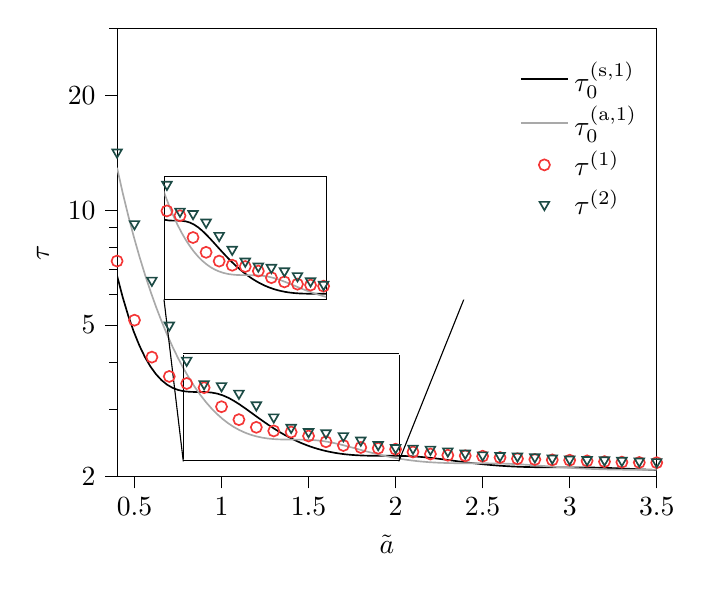
\begin{tikzpicture}

\definecolor{crimson2445454}{RGB}{244,54,54}
\definecolor{darkgray}{RGB}{169,169,169}
\definecolor{darkgray176}{RGB}{176,176,176}
\definecolor{darkslategray287569}{RGB}{28,75,69}

\begin{axis}[
legend cell align={left},
legend style={fill opacity=0.8, draw opacity=1, text opacity=1, at={(0.99,0.95)}, draw=none},
log basis y={10},
tick align=outside,
tick pos=left,
x grid style={darkgray176},
xlabel={\(\displaystyle \tilde{a}\)},
xmin=0.4, xmax=3.5,
xtick style={color=black},
y grid style={darkgray176},
ylabel={\(\displaystyle \tau\)},
ymin=2, ymax=30,
ymode=log,
ytick style={color=black},
log ticks with fixed point, %afegit a ma
ytick={2,5,10,20}, %afegit a ma
minor ytick={3,4,6,7,8,9,30} %afegit a ma
log ticks with fixed point, %afegit a ma
ytick={2,5,10,20}, %afegit a ma
minor ytick={3,4,6,7,8,9,30} %afegit a ma
]
\path [draw=black, very thin]
(axis cs:0.78,2.2)
--(axis cs:2.02,2.2);

\path [draw=black, very thin]
(axis cs:0.78,4.2)
--(axis cs:2.02,4.2);

\addplot [semithick, black]
table {%
0.4 6.72825292030247
0.432 5.91545229187631
0.464 5.28634768911461
0.496 4.7963421411059
0.528 4.41382951009721
0.56 4.11584473555358
0.592 3.88530443637343
0.624 3.70920029906621
0.656 3.57737918096583
0.688 3.48169197502918
0.72 3.41537700159799
0.752 3.37259296791516
0.784 3.34804790269751
0.816 3.33669479704719
0.848 3.33349139370581
0.88 3.33325966156223
0.912 3.33073157530565
0.944 3.32090257103383
0.976 3.29974467739081
1.008 3.26507155626806
1.04 3.21704435882346
1.072 3.15789236591412
1.104 3.09098926945622
1.136 3.01985541220195
1.168 2.9475167459249
1.2 2.87627377548193
1.232 2.80772899264669
1.264 2.74291813435254
1.296 2.6824556232774
1.328 2.62665822415478
1.36 2.57563908592478
1.392 2.52937532481947
1.424 2.48775507326301
1.456 2.45060957269139
1.488 2.41773469827627
1.52 2.38890511211673
1.552 2.36388328585707
1.584 2.34242493091744
1.616 2.32428187820386
1.648 2.3092031061096
1.68 2.29693438294397
1.712 2.28721683825132
1.744 2.27978469031944
1.776 2.27436233000581
1.808 2.27066100098259
1.84 2.26837544184565
1.872 2.26718109168218
1.904 2.26673282649373
1.936 2.26666666689641
1.968 2.26660634804295
2 2.26617674812126
2.032 2.26502539160133
2.064 2.26285103677499
2.096 2.2594348023592
2.128 2.25466582061739
2.16 2.24855263491284
2.192 2.24121531641575
2.224 2.23286023248796
2.256 2.22374541790808
2.288 2.21414614125772
2.32 2.2043275861464
2.352 2.19452726065865
2.384 2.18494634422811
2.416 2.17574758376365
2.448 2.16705718622216
2.48 2.15896868761904
2.512 2.15154745968379
2.544 2.1448350844609
2.576 2.1388532189681
2.608 2.13360680951658
2.64 2.12908664450602
2.672 2.12527129699727
2.704 2.12212853418087
2.736 2.1196162796304
2.768 2.1176832183426
2.8 2.11626914202972
2.832 2.11530514846053
2.864 2.1147138375684
2.896 2.1144096897957
2.928 2.11429986501649
2.96 2.11428571034752
2.992 2.11426528459169
3.024 2.11413715146644
3.056 2.11380551071437
3.088 2.11318639505667
3.12 2.112214202786
3.152 2.1108474137403
3.184 2.1090721878128
3.216 2.10690285892357
3.248 2.10437908292852
3.28 2.10156027789147
3.312 2.09851861393579
3.344 2.09533193468344
3.376 2.09207767569857
3.408 2.08882832862578
3.44 2.08564852538979
3.472 2.08259351219079
3.504 2.07970865719002
3.536 2.07702963552704
3.568 2.07458299812218
};
\addlegendentry{$\tau_0^{(\text{s},1)}$}
\addplot [semithick, darkgray]
table {%
0.4 12.9162306347444
0.432 11.1138365818156
0.464 9.67730849530524
0.496 8.51575913796571
0.528 7.56497601568763
0.56 6.7785486318439
0.592 6.12225708536105
0.624 5.57042056153321
0.656 5.10346066222428
0.688 4.70623864362572
0.72 4.36689782174188
0.752 4.07604299660612
0.784 3.82614917423807
0.816 3.61112908969108
0.848 3.42601249153608
0.88 3.2667052370696
0.912 3.1298061370274
0.944 3.0124660815167
0.976 2.91227844232942
1.008 2.82719281050617
1.04 2.7554462564738
1.072 2.69550779396016
1.104 2.64603278627069
1.136 2.60582478782342
1.168 2.5738028585519
1.2 2.54897279498128
1.232 2.53040105293274
1.264 2.5171904641607
1.296 2.5084572701833
1.328 2.503309655249
1.36 2.50082905874767
1.392 2.50005730761843
1.424 2.49999509528597
1.456 2.49961999149745
1.488 2.4979330737079
1.52 2.49403875875811
1.552 2.48724900820696
1.584 2.4771833106719
1.616 2.46382330317037
1.648 2.44749238234971
1.68 2.42876510982215
1.712 2.40834337800905
1.744 2.38694246821459
1.776 2.36521257989832
1.808 2.34369935085843
1.84 2.32283392974876
1.872 2.30294037307233
1.904 2.28425071029639
1.936 2.26692173385964
1.968 2.25105051737134
2 2.23668749640584
2.032 2.22384691035999
2.064 2.21251483266037
2.096 2.20265515882993
2.128 2.19421392897559
2.16 2.18712231511291
2.192 2.1812985452701
2.224 2.17664898481449
2.256 2.17306856026799
2.288 2.17044069781571
2.32 2.16863696320288
2.352 2.16751663777266
2.384 2.16692655197903
2.416 2.16670162120932
2.448 2.16666666975037
2.48 2.16664023292646
2.512 2.16644098988545
2.544 2.16589715232683
2.576 2.16485839465466
2.608 2.1632088075805
2.64 2.16087826566535
2.672 2.15784918360246
2.704 2.15415645066909
2.736 2.14988026687069
2.768 2.14513375196332
2.8 2.14004846305914
2.832 2.13476086454704
2.864 2.12940171813846
2.896 2.12408905353873
2.928 2.11892440630628
2.96 2.11399153860285
2.992 2.10935678505951
3.024 2.10507030442822
3.056 2.10116772061188
3.088 2.09767182360002
3.12 2.09459414287549
3.152 2.09193630203722
3.184 2.08969112355347
3.216 2.0878434883845
3.248 2.08637097666397
3.28 2.08524433024471
3.312 2.08442779111364
3.344 2.08387938517997
3.376 2.08355124084236
3.408 2.08339005601503
3.44 2.08333785250643
3.472 2.0833331741198
3.504 2.08331287912706
3.536 2.0832146275568
3.568 2.0829800486375
};
\addlegendentry{$\tau_0^{(\text{a},1)}$}
\addplot [semithick, crimson2445454, mark=o, mark size=2, mark options={solid,fill opacity=0}, only marks]
table {%
0.4 7.3508
0.5 5.1421
0.6 4.1141
0.7 3.661
0.8 3.509
0.9 3.4212
1 3.0495
1.1 2.8201
1.2 2.6926
1.3 2.6342
1.4 2.6165
1.5 2.5547
1.6 2.4674
1.7 2.4126
1.8 2.3838
1.9 2.3726
2 2.3589
2.1 2.3198
2.2 2.2913
2.3 2.2747
2.4 2.2671
2.5 2.2613
2.6 2.2436
2.7 2.2271
2.8 2.2166
2.9 2.2111
3 2.2074
3.1 2.1986
3.2 2.1885
3.3 2.1815
3.4 2.1773
3.5 2.1745
3.6 2.1695
3.7 2.1632
3.8 2.1582
3.9 2.155
4 2.1527
};
\addlegendentry{$\tau^{(1)}$}
\addplot [semithick, darkslategray287569, mark=triangle, mark size=2, mark options={solid,rotate=180,fill opacity=0}, only marks]
table {%
0.4 14.187
0.5 9.2002
0.6 6.5402
0.7 4.9881
0.8 4.0332
0.9 3.5006
1 3.4572
1.1 3.304
1.2 3.0794
1.3 2.8632
1.4 2.6895
1.5 2.6198
1.6 2.6023
1.7 2.5562
1.8 2.4904
1.9 2.4238
2 2.3785
2.1 2.3709
2.2 2.3566
2.3 2.3312
2.4 2.3009
2.5 2.2755
2.6 2.2679
2.7 2.2617
2.8 2.2499
2.9 2.2343
3 2.2197
3.1 2.213
3.2 2.2092
3.3 2.2029
3.4 2.1941
3.5 2.1852
3.6 2.1798
3.7 2.177
3.8 2.1731
3.9 2.1677
4 2.162
};
\addlegendentry{$\tau^{(2)}$}
\addplot [very thin, black, forget plot]
table {%
0.78 2.22881307097106
0.78 4.17759965032244
};
\addplot [very thin, black, forget plot]
table {%
2.02 2.22881307097106
2.02 4.17759965032244
};
\path [draw=black, fill=black]
(axis cs:0.67,5.8)
--(axis cs:0.67,5.8)
--(axis cs:0.670000499766753,5.80000001527065)
--(axis cs:0.780000499766753,2.20000001527065)
--(axis cs:0.779999500233247,2.19999998472935)
--(axis cs:0.669999500233247,5.79999998472935)
--(axis cs:0.67,5.8)
--cycle;
\path [draw=black, fill=black]
(axis cs:2.39,5.8)
--(axis cs:2.39,5.8)
--(axis cs:2.39000049737992,5.7999999488804)
--(axis cs:2.02000049737992,2.1999999488804)
--(axis cs:2.01999950262008,2.2000000511196)
--(axis cs:2.38999950262008,5.8000000511196)
--(axis cs:2.39,5.8)
--cycle;
\end{axis}

\begin{axis}[
log basis y={10},
xmajorticks=false,
xmin=0.78, xmax=2.02,
ymajorticks=false,
ymin=2.2, ymax=4.2,
ymode=log,
xshift=0.6cm,yshift=2.25cm,width=0.3\textwidth
]
\addplot [semithick, black]
table {%
0.4 6.72825292030247
0.432 5.91545229187631
0.464 5.28634768911461
0.496 4.7963421411059
0.528 4.41382951009721
0.56 4.11584473555358
0.592 3.88530443637343
0.624 3.70920029906621
0.656 3.57737918096583
0.688 3.48169197502918
0.72 3.41537700159799
0.752 3.37259296791516
0.784 3.34804790269751
0.816 3.33669479704719
0.848 3.33349139370581
0.88 3.33325966156223
0.912 3.33073157530565
0.944 3.32090257103383
0.976 3.29974467739081
1.008 3.26507155626806
1.04 3.21704435882346
1.072 3.15789236591412
1.104 3.09098926945622
1.136 3.01985541220195
1.168 2.9475167459249
1.2 2.87627377548193
1.232 2.80772899264669
1.264 2.74291813435254
1.296 2.6824556232774
1.328 2.62665822415478
1.36 2.57563908592478
1.392 2.52937532481947
1.424 2.48775507326301
1.456 2.45060957269139
1.488 2.41773469827627
1.52 2.38890511211673
1.552 2.36388328585707
1.584 2.34242493091744
1.616 2.32428187820386
1.648 2.3092031061096
1.68 2.29693438294397
1.712 2.28721683825132
1.744 2.27978469031944
1.776 2.27436233000581
1.808 2.27066100098259
1.84 2.26837544184565
1.872 2.26718109168218
1.904 2.26673282649373
1.936 2.26666666689641
1.968 2.26660634804295
2 2.26617674812126
2.032 2.26502539160133
2.064 2.26285103677499
2.096 2.2594348023592
2.128 2.25466582061739
2.16 2.24855263491284
2.192 2.24121531641575
2.224 2.23286023248796
2.256 2.22374541790808
2.288 2.21414614125772
2.32 2.2043275861464
2.352 2.19452726065865
2.384 2.18494634422811
2.416 2.17574758376365
2.448 2.16705718622216
2.48 2.15896868761904
2.512 2.15154745968379
2.544 2.1448350844609
2.576 2.1388532189681
2.608 2.13360680951658
2.64 2.12908664450602
2.672 2.12527129699727
2.704 2.12212853418087
2.736 2.1196162796304
2.768 2.1176832183426
2.8 2.11626914202972
2.832 2.11530514846053
2.864 2.1147138375684
2.896 2.1144096897957
2.928 2.11429986501649
2.96 2.11428571034752
2.992 2.11426528459169
3.024 2.11413715146644
3.056 2.11380551071437
3.088 2.11318639505667
3.12 2.112214202786
3.152 2.1108474137403
3.184 2.1090721878128
3.216 2.10690285892357
3.248 2.10437908292852
3.28 2.10156027789147
3.312 2.09851861393579
3.344 2.09533193468344
3.376 2.09207767569857
3.408 2.08882832862578
3.44 2.08564852538979
3.472 2.08259351219079
3.504 2.07970865719002
3.536 2.07702963552704
3.568 2.07458299812218
};
\addplot [semithick, darkgray]
table {%
0.4 12.9162306347444
0.432 11.1138365818156
0.464 9.67730849530524
0.496 8.51575913796571
0.528 7.56497601568763
0.56 6.7785486318439
0.592 6.12225708536105
0.624 5.57042056153321
0.656 5.10346066222428
0.688 4.70623864362572
0.72 4.36689782174188
0.752 4.07604299660612
0.784 3.82614917423807
0.816 3.61112908969108
0.848 3.42601249153608
0.88 3.2667052370696
0.912 3.1298061370274
0.944 3.0124660815167
0.976 2.91227844232942
1.008 2.82719281050617
1.04 2.7554462564738
1.072 2.69550779396016
1.104 2.64603278627069
1.136 2.60582478782342
1.168 2.5738028585519
1.2 2.54897279498128
1.232 2.53040105293274
1.264 2.5171904641607
1.296 2.5084572701833
1.328 2.503309655249
1.36 2.50082905874767
1.392 2.50005730761843
1.424 2.49999509528597
1.456 2.49961999149745
1.488 2.4979330737079
1.52 2.49403875875811
1.552 2.48724900820696
1.584 2.4771833106719
1.616 2.46382330317037
1.648 2.44749238234971
1.68 2.42876510982215
1.712 2.40834337800905
1.744 2.38694246821459
1.776 2.36521257989832
1.808 2.34369935085843
1.84 2.32283392974876
1.872 2.30294037307233
1.904 2.28425071029639
1.936 2.26692173385964
1.968 2.25105051737134
2 2.23668749640584
2.032 2.22384691035999
2.064 2.21251483266037
2.096 2.20265515882993
2.128 2.19421392897559
2.16 2.18712231511291
2.192 2.1812985452701
2.224 2.17664898481449
2.256 2.17306856026799
2.288 2.17044069781571
2.32 2.16863696320288
2.352 2.16751663777266
2.384 2.16692655197903
2.416 2.16670162120932
2.448 2.16666666975037
2.48 2.16664023292646
2.512 2.16644098988545
2.544 2.16589715232683
2.576 2.16485839465466
2.608 2.1632088075805
2.64 2.16087826566535
2.672 2.15784918360246
2.704 2.15415645066909
2.736 2.14988026687069
2.768 2.14513375196332
2.8 2.14004846305914
2.832 2.13476086454704
2.864 2.12940171813846
2.896 2.12408905353873
2.928 2.11892440630628
2.96 2.11399153860285
2.992 2.10935678505951
3.024 2.10507030442822
3.056 2.10116772061188
3.088 2.09767182360002
3.12 2.09459414287549
3.152 2.09193630203722
3.184 2.08969112355347
3.216 2.0878434883845
3.248 2.08637097666397
3.28 2.08524433024471
3.312 2.08442779111364
3.344 2.08387938517997
3.376 2.08355124084236
3.408 2.08339005601503
3.44 2.08333785250643
3.472 2.0833331741198
3.504 2.08331287912706
3.536 2.0832146275568
3.568 2.0829800486375
};
\addplot [semithick, crimson2445454, mark=o, mark size=2, mark options={solid,fill opacity=0}, only marks]
table {%
0.4 7.3508
0.5 5.1421
0.6 4.1141
0.7 3.661
0.8 3.509
0.9 3.4212
1 3.0495
1.1 2.8201
1.2 2.6926
1.3 2.6342
1.4 2.6165
1.5 2.5547
1.6 2.4674
1.7 2.4126
1.8 2.3838
1.9 2.3726
2 2.3589
2.1 2.3198
2.2 2.2913
2.3 2.2747
2.4 2.2671
2.5 2.2613
2.6 2.2436
2.7 2.2271
2.8 2.2166
2.9 2.2111
3 2.2074
3.1 2.1986
3.2 2.1885
3.3 2.1815
3.4 2.1773
3.5 2.1745
3.6 2.1695
3.7 2.1632
3.8 2.1582
3.9 2.155
4 2.1527
};
\addplot [semithick, darkslategray287569, mark=triangle, mark size=2, mark options={solid,rotate=180,fill opacity=0}, only marks]
table {%
0.4 14.187
0.5 9.2002
0.6 6.5402
0.7 4.9881
0.8 4.0332
0.9 3.5006
1 3.4572
1.1 3.304
1.2 3.0794
1.3 2.8632
1.4 2.6895
1.5 2.6198
1.6 2.6023
1.7 2.5562
1.8 2.4904
1.9 2.4238
2 2.3785
2.1 2.3709
2.2 2.3566
2.3 2.3312
2.4 2.3009
2.5 2.2755
2.6 2.2679
2.7 2.2617
2.8 2.2499
2.9 2.2343
3 2.2197
3.1 2.213
3.2 2.2092
3.3 2.2029
3.4 2.1941
3.5 2.1852
3.6 2.1798
3.7 2.177
3.8 2.1731
3.9 2.1677
4 2.162
};
\end{axis}

\end{tikzpicture}

% This file was created with tikzplotlib v0.10.1.
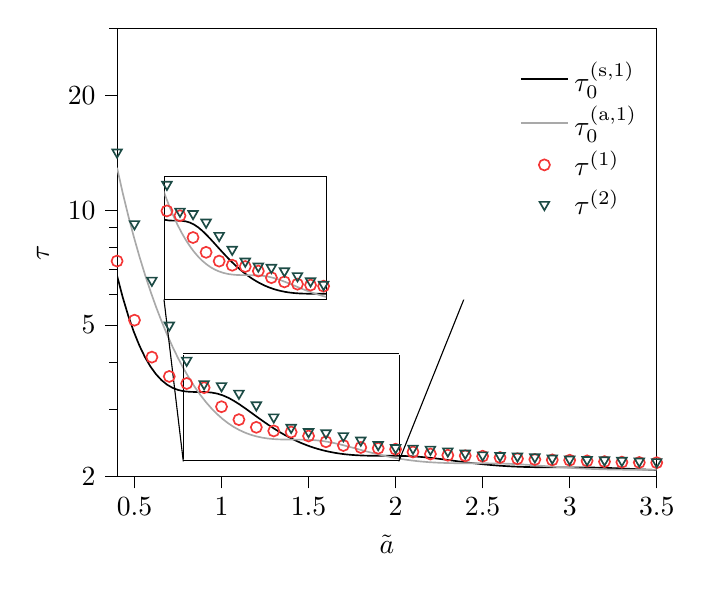
\begin{tikzpicture}

\definecolor{crimson2445454}{RGB}{244,54,54}
\definecolor{darkgray}{RGB}{169,169,169}
\definecolor{darkgray176}{RGB}{176,176,176}
\definecolor{darkslategray287569}{RGB}{28,75,69}

\begin{axis}[
legend cell align={left},
legend style={fill opacity=0.8, draw opacity=1, text opacity=1, at={(0.99,0.95)}, draw=none},
log basis y={10},
tick align=outside,
tick pos=left,
x grid style={darkgray176},
xlabel={\(\displaystyle \tilde{a}\)},
xmin=0.4, xmax=3.5,
xtick style={color=black},
y grid style={darkgray176},
ylabel={\(\displaystyle \tau\)},
ymin=2, ymax=30,
ymode=log,
ytick style={color=black},
log ticks with fixed point, %afegit a ma
ytick={2,5,10,20}, %afegit a ma
minor ytick={3,4,6,7,8,9,30} %afegit a ma
log ticks with fixed point, %afegit a ma
ytick={2,5,10,20}, %afegit a ma
minor ytick={3,4,6,7,8,9,30} %afegit a ma
]
\path [draw=black, very thin]
(axis cs:0.78,2.2)
--(axis cs:2.02,2.2);

\path [draw=black, very thin]
(axis cs:0.78,4.2)
--(axis cs:2.02,4.2);

\addplot [semithick, black]
table {%
0.4 6.72825292030247
0.432 5.91545229187631
0.464 5.28634768911461
0.496 4.7963421411059
0.528 4.41382951009721
0.56 4.11584473555358
0.592 3.88530443637343
0.624 3.70920029906621
0.656 3.57737918096583
0.688 3.48169197502918
0.72 3.41537700159799
0.752 3.37259296791516
0.784 3.34804790269751
0.816 3.33669479704719
0.848 3.33349139370581
0.88 3.33325966156223
0.912 3.33073157530565
0.944 3.32090257103383
0.976 3.29974467739081
1.008 3.26507155626806
1.04 3.21704435882346
1.072 3.15789236591412
1.104 3.09098926945622
1.136 3.01985541220195
1.168 2.9475167459249
1.2 2.87627377548193
1.232 2.80772899264669
1.264 2.74291813435254
1.296 2.6824556232774
1.328 2.62665822415478
1.36 2.57563908592478
1.392 2.52937532481947
1.424 2.48775507326301
1.456 2.45060957269139
1.488 2.41773469827627
1.52 2.38890511211673
1.552 2.36388328585707
1.584 2.34242493091744
1.616 2.32428187820386
1.648 2.3092031061096
1.68 2.29693438294397
1.712 2.28721683825132
1.744 2.27978469031944
1.776 2.27436233000581
1.808 2.27066100098259
1.84 2.26837544184565
1.872 2.26718109168218
1.904 2.26673282649373
1.936 2.26666666689641
1.968 2.26660634804295
2 2.26617674812126
2.032 2.26502539160133
2.064 2.26285103677499
2.096 2.2594348023592
2.128 2.25466582061739
2.16 2.24855263491284
2.192 2.24121531641575
2.224 2.23286023248796
2.256 2.22374541790808
2.288 2.21414614125772
2.32 2.2043275861464
2.352 2.19452726065865
2.384 2.18494634422811
2.416 2.17574758376365
2.448 2.16705718622216
2.48 2.15896868761904
2.512 2.15154745968379
2.544 2.1448350844609
2.576 2.1388532189681
2.608 2.13360680951658
2.64 2.12908664450602
2.672 2.12527129699727
2.704 2.12212853418087
2.736 2.1196162796304
2.768 2.1176832183426
2.8 2.11626914202972
2.832 2.11530514846053
2.864 2.1147138375684
2.896 2.1144096897957
2.928 2.11429986501649
2.96 2.11428571034752
2.992 2.11426528459169
3.024 2.11413715146644
3.056 2.11380551071437
3.088 2.11318639505667
3.12 2.112214202786
3.152 2.1108474137403
3.184 2.1090721878128
3.216 2.10690285892357
3.248 2.10437908292852
3.28 2.10156027789147
3.312 2.09851861393579
3.344 2.09533193468344
3.376 2.09207767569857
3.408 2.08882832862578
3.44 2.08564852538979
3.472 2.08259351219079
3.504 2.07970865719002
3.536 2.07702963552704
3.568 2.07458299812218
};
\addlegendentry{$\tau_0^{(\text{s},1)}$}
\addplot [semithick, darkgray]
table {%
0.4 12.9162306347444
0.432 11.1138365818156
0.464 9.67730849530524
0.496 8.51575913796571
0.528 7.56497601568763
0.56 6.7785486318439
0.592 6.12225708536105
0.624 5.57042056153321
0.656 5.10346066222428
0.688 4.70623864362572
0.72 4.36689782174188
0.752 4.07604299660612
0.784 3.82614917423807
0.816 3.61112908969108
0.848 3.42601249153608
0.88 3.2667052370696
0.912 3.1298061370274
0.944 3.0124660815167
0.976 2.91227844232942
1.008 2.82719281050617
1.04 2.7554462564738
1.072 2.69550779396016
1.104 2.64603278627069
1.136 2.60582478782342
1.168 2.5738028585519
1.2 2.54897279498128
1.232 2.53040105293274
1.264 2.5171904641607
1.296 2.5084572701833
1.328 2.503309655249
1.36 2.50082905874767
1.392 2.50005730761843
1.424 2.49999509528597
1.456 2.49961999149745
1.488 2.4979330737079
1.52 2.49403875875811
1.552 2.48724900820696
1.584 2.4771833106719
1.616 2.46382330317037
1.648 2.44749238234971
1.68 2.42876510982215
1.712 2.40834337800905
1.744 2.38694246821459
1.776 2.36521257989832
1.808 2.34369935085843
1.84 2.32283392974876
1.872 2.30294037307233
1.904 2.28425071029639
1.936 2.26692173385964
1.968 2.25105051737134
2 2.23668749640584
2.032 2.22384691035999
2.064 2.21251483266037
2.096 2.20265515882993
2.128 2.19421392897559
2.16 2.18712231511291
2.192 2.1812985452701
2.224 2.17664898481449
2.256 2.17306856026799
2.288 2.17044069781571
2.32 2.16863696320288
2.352 2.16751663777266
2.384 2.16692655197903
2.416 2.16670162120932
2.448 2.16666666975037
2.48 2.16664023292646
2.512 2.16644098988545
2.544 2.16589715232683
2.576 2.16485839465466
2.608 2.1632088075805
2.64 2.16087826566535
2.672 2.15784918360246
2.704 2.15415645066909
2.736 2.14988026687069
2.768 2.14513375196332
2.8 2.14004846305914
2.832 2.13476086454704
2.864 2.12940171813846
2.896 2.12408905353873
2.928 2.11892440630628
2.96 2.11399153860285
2.992 2.10935678505951
3.024 2.10507030442822
3.056 2.10116772061188
3.088 2.09767182360002
3.12 2.09459414287549
3.152 2.09193630203722
3.184 2.08969112355347
3.216 2.0878434883845
3.248 2.08637097666397
3.28 2.08524433024471
3.312 2.08442779111364
3.344 2.08387938517997
3.376 2.08355124084236
3.408 2.08339005601503
3.44 2.08333785250643
3.472 2.0833331741198
3.504 2.08331287912706
3.536 2.0832146275568
3.568 2.0829800486375
};
\addlegendentry{$\tau_0^{(\text{a},1)}$}
\addplot [semithick, crimson2445454, mark=o, mark size=2, mark options={solid,fill opacity=0}, only marks]
table {%
0.4 7.3508
0.5 5.1421
0.6 4.1141
0.7 3.661
0.8 3.509
0.9 3.4212
1 3.0495
1.1 2.8201
1.2 2.6926
1.3 2.6342
1.4 2.6165
1.5 2.5547
1.6 2.4674
1.7 2.4126
1.8 2.3838
1.9 2.3726
2 2.3589
2.1 2.3198
2.2 2.2913
2.3 2.2747
2.4 2.2671
2.5 2.2613
2.6 2.2436
2.7 2.2271
2.8 2.2166
2.9 2.2111
3 2.2074
3.1 2.1986
3.2 2.1885
3.3 2.1815
3.4 2.1773
3.5 2.1745
3.6 2.1695
3.7 2.1632
3.8 2.1582
3.9 2.155
4 2.1527
};
\addlegendentry{$\tau^{(1)}$}
\addplot [semithick, darkslategray287569, mark=triangle, mark size=2, mark options={solid,rotate=180,fill opacity=0}, only marks]
table {%
0.4 14.187
0.5 9.2002
0.6 6.5402
0.7 4.9881
0.8 4.0332
0.9 3.5006
1 3.4572
1.1 3.304
1.2 3.0794
1.3 2.8632
1.4 2.6895
1.5 2.6198
1.6 2.6023
1.7 2.5562
1.8 2.4904
1.9 2.4238
2 2.3785
2.1 2.3709
2.2 2.3566
2.3 2.3312
2.4 2.3009
2.5 2.2755
2.6 2.2679
2.7 2.2617
2.8 2.2499
2.9 2.2343
3 2.2197
3.1 2.213
3.2 2.2092
3.3 2.2029
3.4 2.1941
3.5 2.1852
3.6 2.1798
3.7 2.177
3.8 2.1731
3.9 2.1677
4 2.162
};
\addlegendentry{$\tau^{(2)}$}
\addplot [very thin, black, forget plot]
table {%
0.78 2.22881307097106
0.78 4.17759965032244
};
\addplot [very thin, black, forget plot]
table {%
2.02 2.22881307097106
2.02 4.17759965032244
};
\path [draw=black, fill=black]
(axis cs:0.67,5.8)
--(axis cs:0.67,5.8)
--(axis cs:0.670000499766753,5.80000001527065)
--(axis cs:0.780000499766753,2.20000001527065)
--(axis cs:0.779999500233247,2.19999998472935)
--(axis cs:0.669999500233247,5.79999998472935)
--(axis cs:0.67,5.8)
--cycle;
\path [draw=black, fill=black]
(axis cs:2.39,5.8)
--(axis cs:2.39,5.8)
--(axis cs:2.39000049737992,5.7999999488804)
--(axis cs:2.02000049737992,2.1999999488804)
--(axis cs:2.01999950262008,2.2000000511196)
--(axis cs:2.38999950262008,5.8000000511196)
--(axis cs:2.39,5.8)
--cycle;
\end{axis}

\begin{axis}[
log basis y={10},
xmajorticks=false,
xmin=0.78, xmax=2.02,
ymajorticks=false,
ymin=2.2, ymax=4.2,
ymode=log,
xshift=0.6cm,yshift=2.25cm,width=0.3\textwidth
]
\addplot [semithick, black]
table {%
0.4 6.72825292030247
0.432 5.91545229187631
0.464 5.28634768911461
0.496 4.7963421411059
0.528 4.41382951009721
0.56 4.11584473555358
0.592 3.88530443637343
0.624 3.70920029906621
0.656 3.57737918096583
0.688 3.48169197502918
0.72 3.41537700159799
0.752 3.37259296791516
0.784 3.34804790269751
0.816 3.33669479704719
0.848 3.33349139370581
0.88 3.33325966156223
0.912 3.33073157530565
0.944 3.32090257103383
0.976 3.29974467739081
1.008 3.26507155626806
1.04 3.21704435882346
1.072 3.15789236591412
1.104 3.09098926945622
1.136 3.01985541220195
1.168 2.9475167459249
1.2 2.87627377548193
1.232 2.80772899264669
1.264 2.74291813435254
1.296 2.6824556232774
1.328 2.62665822415478
1.36 2.57563908592478
1.392 2.52937532481947
1.424 2.48775507326301
1.456 2.45060957269139
1.488 2.41773469827627
1.52 2.38890511211673
1.552 2.36388328585707
1.584 2.34242493091744
1.616 2.32428187820386
1.648 2.3092031061096
1.68 2.29693438294397
1.712 2.28721683825132
1.744 2.27978469031944
1.776 2.27436233000581
1.808 2.27066100098259
1.84 2.26837544184565
1.872 2.26718109168218
1.904 2.26673282649373
1.936 2.26666666689641
1.968 2.26660634804295
2 2.26617674812126
2.032 2.26502539160133
2.064 2.26285103677499
2.096 2.2594348023592
2.128 2.25466582061739
2.16 2.24855263491284
2.192 2.24121531641575
2.224 2.23286023248796
2.256 2.22374541790808
2.288 2.21414614125772
2.32 2.2043275861464
2.352 2.19452726065865
2.384 2.18494634422811
2.416 2.17574758376365
2.448 2.16705718622216
2.48 2.15896868761904
2.512 2.15154745968379
2.544 2.1448350844609
2.576 2.1388532189681
2.608 2.13360680951658
2.64 2.12908664450602
2.672 2.12527129699727
2.704 2.12212853418087
2.736 2.1196162796304
2.768 2.1176832183426
2.8 2.11626914202972
2.832 2.11530514846053
2.864 2.1147138375684
2.896 2.1144096897957
2.928 2.11429986501649
2.96 2.11428571034752
2.992 2.11426528459169
3.024 2.11413715146644
3.056 2.11380551071437
3.088 2.11318639505667
3.12 2.112214202786
3.152 2.1108474137403
3.184 2.1090721878128
3.216 2.10690285892357
3.248 2.10437908292852
3.28 2.10156027789147
3.312 2.09851861393579
3.344 2.09533193468344
3.376 2.09207767569857
3.408 2.08882832862578
3.44 2.08564852538979
3.472 2.08259351219079
3.504 2.07970865719002
3.536 2.07702963552704
3.568 2.07458299812218
};
\addplot [semithick, darkgray]
table {%
0.4 12.9162306347444
0.432 11.1138365818156
0.464 9.67730849530524
0.496 8.51575913796571
0.528 7.56497601568763
0.56 6.7785486318439
0.592 6.12225708536105
0.624 5.57042056153321
0.656 5.10346066222428
0.688 4.70623864362572
0.72 4.36689782174188
0.752 4.07604299660612
0.784 3.82614917423807
0.816 3.61112908969108
0.848 3.42601249153608
0.88 3.2667052370696
0.912 3.1298061370274
0.944 3.0124660815167
0.976 2.91227844232942
1.008 2.82719281050617
1.04 2.7554462564738
1.072 2.69550779396016
1.104 2.64603278627069
1.136 2.60582478782342
1.168 2.5738028585519
1.2 2.54897279498128
1.232 2.53040105293274
1.264 2.5171904641607
1.296 2.5084572701833
1.328 2.503309655249
1.36 2.50082905874767
1.392 2.50005730761843
1.424 2.49999509528597
1.456 2.49961999149745
1.488 2.4979330737079
1.52 2.49403875875811
1.552 2.48724900820696
1.584 2.4771833106719
1.616 2.46382330317037
1.648 2.44749238234971
1.68 2.42876510982215
1.712 2.40834337800905
1.744 2.38694246821459
1.776 2.36521257989832
1.808 2.34369935085843
1.84 2.32283392974876
1.872 2.30294037307233
1.904 2.28425071029639
1.936 2.26692173385964
1.968 2.25105051737134
2 2.23668749640584
2.032 2.22384691035999
2.064 2.21251483266037
2.096 2.20265515882993
2.128 2.19421392897559
2.16 2.18712231511291
2.192 2.1812985452701
2.224 2.17664898481449
2.256 2.17306856026799
2.288 2.17044069781571
2.32 2.16863696320288
2.352 2.16751663777266
2.384 2.16692655197903
2.416 2.16670162120932
2.448 2.16666666975037
2.48 2.16664023292646
2.512 2.16644098988545
2.544 2.16589715232683
2.576 2.16485839465466
2.608 2.1632088075805
2.64 2.16087826566535
2.672 2.15784918360246
2.704 2.15415645066909
2.736 2.14988026687069
2.768 2.14513375196332
2.8 2.14004846305914
2.832 2.13476086454704
2.864 2.12940171813846
2.896 2.12408905353873
2.928 2.11892440630628
2.96 2.11399153860285
2.992 2.10935678505951
3.024 2.10507030442822
3.056 2.10116772061188
3.088 2.09767182360002
3.12 2.09459414287549
3.152 2.09193630203722
3.184 2.08969112355347
3.216 2.0878434883845
3.248 2.08637097666397
3.28 2.08524433024471
3.312 2.08442779111364
3.344 2.08387938517997
3.376 2.08355124084236
3.408 2.08339005601503
3.44 2.08333785250643
3.472 2.0833331741198
3.504 2.08331287912706
3.536 2.0832146275568
3.568 2.0829800486375
};
\addplot [semithick, crimson2445454, mark=o, mark size=2, mark options={solid,fill opacity=0}, only marks]
table {%
0.4 7.3508
0.5 5.1421
0.6 4.1141
0.7 3.661
0.8 3.509
0.9 3.4212
1 3.0495
1.1 2.8201
1.2 2.6926
1.3 2.6342
1.4 2.6165
1.5 2.5547
1.6 2.4674
1.7 2.4126
1.8 2.3838
1.9 2.3726
2 2.3589
2.1 2.3198
2.2 2.2913
2.3 2.2747
2.4 2.2671
2.5 2.2613
2.6 2.2436
2.7 2.2271
2.8 2.2166
2.9 2.2111
3 2.2074
3.1 2.1986
3.2 2.1885
3.3 2.1815
3.4 2.1773
3.5 2.1745
3.6 2.1695
3.7 2.1632
3.8 2.1582
3.9 2.155
4 2.1527
};
\addplot [semithick, darkslategray287569, mark=triangle, mark size=2, mark options={solid,rotate=180,fill opacity=0}, only marks]
table {%
0.4 14.187
0.5 9.2002
0.6 6.5402
0.7 4.9881
0.8 4.0332
0.9 3.5006
1 3.4572
1.1 3.304
1.2 3.0794
1.3 2.8632
1.4 2.6895
1.5 2.6198
1.6 2.6023
1.7 2.5562
1.8 2.4904
1.9 2.4238
2 2.3785
2.1 2.3709
2.2 2.3566
2.3 2.3312
2.4 2.3009
2.5 2.2755
2.6 2.2679
2.7 2.2617
2.8 2.2499
2.9 2.2343
3 2.2197
3.1 2.213
3.2 2.2092
3.3 2.2029
3.4 2.1941
3.5 2.1852
3.6 2.1798
3.7 2.177
3.8 2.1731
3.9 2.1677
4 2.162
};
\end{axis}

\end{tikzpicture}

	\caption{Critical compression of a stiffened inhomogeneous sheet ($\phiend=0.2,\,\gamma\prime=10$) as a function of the sheet size $\tL$, with numerical results using {\it Chebfun}~\cite{Chebfun} ($\tauu,\taud$). The quantities $\tau_0^{(\text{s})}$, $\tau_0^{(\text{a})}$ denote the smallest pair of compressions of the corresponding homogeneous sheet ($\phiend=0$). Here, the critical compression $\tau$ has been rescaled by the square root of the mean Young's modulus, $\tau/\sqrt{\bar{E}}$, to facilitate comparison with the results from the homoegenous case (solid curves).} 
	\label{soft-res:tau}
\end{figure}

We examine in Fig.~\ref{soft-res:tau} the two smallest compressions of inhomogeneous sheets as the sheet size varies. We use the rescaling $\tau/\sqrt{\bar{E}}$ ($\bar{E}$ denotes the spatial average of Eq.~\eqref{composite:Ec_DT}) in the inhomogeneous case and include for comparison the smallest pair of critical buckling compressions from the homogeneous sheet. We note that this scaling collapses the inhomogeneous case onto the homogeneous case. However, by blowing up the region around $\tL=\tL_{1,1}^{\text{(II)}}$ (see the inset in Fig.~\ref{soft-res:tau}, in which the inhomogeneous curves are computed every $\Delta\tL=0.032$), we see that the compressions of the inhomogeneous sheet do not cross. In other words, they are ordered from smaller to larger for any finite $\tL$. We thus denote the two smallest compressions $\tauu(\tilde{L})$ and $\taud(\tilde{L})$, with $\tauu(\tilde{L})<\taud(\tilde{L})$. Importantly, $\tauu(\tilde{L})$ is larger than the smallest compression in the first pair $(\tau_0^{(\text{s})}, \tau_0^{(\text{a})})$, and hence an inhomogeneous stiffness induces larger compressive loads; at most,  compressions that match the homogeneous counterpart are observed for certain values of $\tL$.

In a thought experiment in which we infinitesimally increase $\phiend$, starting at $\phiend=0$, i.e.~a homogeneous sheet, the intersecting compressions at $\tL$ given by Eqs.~\eqref{finite-size:crossing1} and~\eqref{finite-size:crossing2} split when $\phiend>0$. We measure this separation between consecutive compressions,  and we examine its growth with $\phiend$ close to the corresponding crossing points of the homogeneous sheet, in Fig.~\ref{soft-res:dtmin}. 

We fix $\phiend$ and then we find numerically the local minima of $\Delta\tau^{(2-1)}$ with respect to $\tL$, which we denote $\Delta\tau^{(2-1)}_{\text{min}}$. The values of $\tL$ that minimize $\Delta\tau^{(2-1)}$ start at the crossing points when $\phiend=0$, and increase with $\phiend$. The first eight results $\Delta\tau^{(2-1)}_{\text{min}}$ (corresponding to the first eight crossings in the homogeneous case) are plotted in Fig.~\ref{soft-res:dtmin} for different values of $\phiend/L$, where $L$ is the corresponding sheet size that minimizes $\Delta\tau^{(2-1)}$. All curves $\Delta\tau^{(2-1)}_{\text{min}}$ collapse into one. Therefore we conclude that $\Delta\tau^{(2-1)}_{\text{min}}$ grows linearly with $\phiend/L$, which is % twice the amplitude of 
the gradient from Eq.~\eqref{buckle:phi}.

\begin{figure}
	%\includegraphics[width=\columnwidth]{figures/fig_splitting/plDeltatauMinNUMscaledLog.eps}
	\includegraphics[width=\columnwidth]{plDeltatauMinNUMscaledLog.eps}
	\caption{Minimal separation between the two smallest compressions %$\Delta\tau=\tau^{(2)}-\tau^{(1)}$
	$\Delta\tau_{\text{min}}^{(2-1)}$ of a stiffened inhomogeneous sheet ($\gamma\prime=10$). Different symbols denote those minima corresponding to the crossings of type I (circles), and of type II (triangles) when $\phiend/L=0$. Shades of gray correspond to the crossing point index $l$: lighter gray for $l=1$, darkest gray for $l=4$. The red right triangle is one decade in length on both legs showing the linear relation %$\Delta\tau\propto\phiend/L$
	$\Delta\tau_{\text{min}}^{(2-1)}\propto\phiend/L$.}
\label{soft-res:dtmin}
\end{figure}


\section{Conclusions\label{sec:conclusions}}
We have examined the two--dimensional buckling and wrinkle patterns in floating homogeneous and inhomogeneous thin elastic sheets. With two control parameters, the size of the confined sheet and the gradient of bending stiffness, we quantified the wrinkled states using the F\"{o}ppl--von K\'{a}rm\'{a}n theory of thin sheets. A central test of the results is to vary the bending stiffness by varying the volume fraction of inclusions in the host solid. 

In homogeneous sheets, the only control parameter is the sheet size $L$. The buckling profile is determined by the smallest compressive load, and so we expect that the mode that will be observed in a buckling experiment corresponds to the smallest compression. However, for some particular sizes of the confined sheet, the same compression is associated with two different wrinkling modes. We gave asymptotic results for the shape of the sheet at  the onset of buckling, together with the critical loads and the critical sheet sizes for degeneracy in the limit of large sheets, $L\gg1$.

In contrast, this degeneracy is not observed in inhomogeneous sheets. Indeed, the otherwise crossing compressions of the homogeneous case split when a gradient of stiffness is applied parallel to the direction of confinement. The size of this splitting grows linearly with the magnitude of the gradient of the volume fraction at all the crossing points. Importantly, the wrinkled states of confined inhomogeneous sheets depend sensitively on their size. While medium length sheets buckle very much like their homogeneous counterparts, the wrinkled states in large length sheets are a superposition of many modes. This feature of large length sheets allows for the bending energy to be spatially concentrated, which is crucial in establishing a failure criterion, with particular relevance in glaciology.

Finally, the results presented here for floating sheets are also relevant for sheets on a linear soft elastic foundation,~\cite[see e.g.~Ref.][]{HuntWadee93}. A more complex behaviour is expected in the more general case of a linear elastic foundation, whose response is expected to be geometrically nonlinear, in which localization of buckling occurs,~\cite[see e.g., Ref.][]{Potier-Ferry1983,Brau2011}. In addition to the range of applications of interest, from soft composites of biological relevance \cite{GorielyBook} to hard composites of engineering or geophysical importance, a thorough mathematical analysis, rather than the numerical study given here, may provide additional insights. 

\begin{acknowledgements}
We thank A. Souslov and D. Mitra for helpful comments. MS, AFB and JSW acknowledge the support of Swedish Research Council Grant No. 638-2013-9243. CA acknowledges the support of the Swedish Research Council Grant No. 2018-04290. Nordita is partially supported by Nordforsk.
\end{acknowledgements}

\appendix
\begin{widetext}


\section{Details of theoretical formulation \label{App:GovEqn}}

 In the main text, we gave the equation governing the out-of-plane displacement of the beam without a formal derivation. Here, we expand upon the derivation of this.  A key detail concerns the state of stress within the sheet --- to ensure that this stress satisfies in-plane equilibrium, $\nabla\cdot\mathbf{\sigma}^*=0$, we introduce a force function $\varphi^*$: the internal in--plane forces per unit length are obtained by double differentiation of $\varphi^*$ so that $\sigma_{xx}^*=\partial^2\varphi^*/\partial y^{*2}$, $\sigma_{yy}^*=\partial^2\varphi^*/\partial x^{*2}$ and $\sigma_{xy}^*=-\partial^2\varphi^*/\partial x^*\partial y^*$ ~\cite{Mansfield}.  Following the standard derivation of the plate equation, see~\cite{Mansfield}, but accounting for the possibility that $\nu=\nu(x^*)$, we find that normal displacements of the sheet satisfy:
\be
	\nabla^2(B^*(x^*)\nabla^2 w^*)-[B^*(x^*)\{1-\nu(x^*)\},w^*]+\rho^*g^*w^*=[w^*,\varphi^*],
        \label{mech:gov}
\ee where $B^*(x^*)$ is the bending stiffness (or flexural rigidity) of the sheet and the von K\'{a}rm\'{a}n operator is
\be
    [w^*,\varphi^*]\equiv\pdTwo{w^*}{{x^*}}\pdTwo{\varphi^*}{{y^*}}-2\frac{\pd^2w^*}{\pd x^*\pd y^*}\frac{\pd^2\varphi^*}{\pd x^*\pd y^*}+\pdTwo{w^*}{{y^*}} \pdTwo{\varphi^*}{{x^*}}.
\label{mech:dieop}
\ee

For a midplane displacement with components $(u^*,v^*,w^*)$, the sheet's in--plane strains, $\epsilon_{ij}$, are given by
\begin{align}
        \epsilon_{x^*x^*}&=(u^*)_{,x^*}+\tfrac{1}{2}(w^*)_{,x^*}^2,\quad\epsilon_{y^*y^*}=(v^*)_{,y^*}+\tfrac{1}{2}(w^*)_{,y^*}^2,\nonumber \\
        \textrm{and}& \quad \epsilon_{x^*y^*}=\tfrac{1}{2}[(u^*)_{,y^*}+(v^*)_{,x^*}+(w^*)_{,x^*}(w^*)_{,y^*}],
\label{mech:strains}
\end{align} 
where, for example, $(w^*)_{,x^*}$ denotes the partial derivative of $w^*$ with respect to $x^*$. Note that the displacements $u^*$ and $v^*$ may be eliminated from these relationships by cross-differentiation,~\cite[see pg. 13 of Ref.~][]{Mansfield}. Relating these derivatives of strains to the in-plane forces, and hence to the derivatives of the force function $\varphi^*$, one finds the compatibility equation
\be
        \nabla^2\left(\frac{1}{E^*(x^*)}\nabla^2\varphi^*\right)-\left[\frac{1+\nu(x^*)}{E^*(x^*)},\varphi^*\right]=-\frac{h^*}{2}[w^*,w^*],\label{mech:eq_comp}
\ee
which gives the stress in the plane of the sheet induced by the stretching of the sheet's mid-plane.

In the two-dimensional buckling problem shown schematically in Figure \ref{mech:schema}, there are no variations in the $y^*$ direction (i.e.~into the page). Therefore, the vertical displacement of the sheet, $w^*$, is independent of $y^*$ and equations \eqref{mech:gov} and \eqref{mech:eq_comp} simplify to the following system;
\begin{subequations}
\begin{align}
	\frac{\mathrm{d}^2}{\mathrm{d}x^{*2}}\Bigl[B^*(x^*) w^*_{,2x^*}\Bigr]+w^*&=\varphi^*_{,2y^*}w^*_{,2x^*},\label{buckle:fvk:1}\\
	\textrm{and} \quad \nabla^2\left(\frac{1}{E^*(x^*)}\nabla^2\varphi^*\right)&=0.
\label{buckle:fvk:2}
\end{align}
\label{buckle:fvk}
\end{subequations}
Now, because $w^*=w^*(x^*)$ then $\varphi^*_{,2y^*}=f(x^*)$, so that $\varphi^*_{,x^*y^*}=A(x^*)+y^*f'(x^*)$. However, $\varphi^*_{,x^*y^*}$ is just the traction exerted on the sheet in the $y^*$ direction. This traction is zero for compression purely in the $x^*$ direction, so we have $f'(x^*)=0$, and hence $f(x^*)$ is a constant. Since the compressive load at the boundary $x^*=L^*/2$
%a$ ($a\equiv a^*/\ell^*$)
is in the $x^*$ direction, and has magnitude $\tau^*$
%$\tau\equiv \tau^* (\ell^*)^2/B_{0}^*$, we must have
\begin{align}
        \varphi^*_{,2y^*}(x^*=L^*/2)=-\tau^*,
\end{align}
and so that $f(x^*)=-\tau^*$. Thus Eq.~\eqref{buckle:fvk:1} becomes
\begin{equation}
        \frac{\mathrm{d}^2}{\mathrm{d}x^{*2}}\left[B^*(x^*) w^*_{,2x^*}\right]+\tau^* w^*_{,2x^*}+w^*=0,
\label{buckle:ode}
\end{equation}
which is Euler's linearized elastica equation \cite[see e.g. \S 20 of Ref.~][]{LandauLifshitz86} with a lateral load due to the hydrostatic pressure in the liquid foundation and varying elastic properties along the axis of confinement.
The boundaries of the thin sheet at $x^*=\pm L^*/2$ are clamped so that $w^*_{,x^*}(\pm L^*/2)=w^*(\pm L^*/2)=0$.


\section{Effective stiffness of composite materials \label{AppA}}
The foundational Eshelby theory of solid composites~\cite{Eshelby57} describes the elastic behaviour of rigid composites with a dilute dispersion of noninteracting incompressible inclusions.
Stiff-matrix materials such as ice, glass, ceramics and steel have $E^*=O(\text{GPa})$ and $\nu\sim0.3$, and thus have subnanometric elastocapillary length.  Therefore, for typical inclusion sizes the effect of surface tension is negligible and we can use Eshelby theory~\cite{Eshelby57} to compute the effective elastic moduli of compression, $\kappa^*$, and rigidity, $\mu^*$, which are
\begin{align}
        \kappa^*&=\kappa_{0}^*\left\{1- \left[\frac{(\kappa_{1}^*-\kappa_{0}^*)}{(\kappa_{0}^*-\kappa_{1}^*)\alpha-\kappa_{0}^*}\right]\phi\right\},~\text{and}\nonumber\\
        \mu^*&=\mu_{0}^*\left\{1-\left[\frac{\mu_{1}^*-\mu_{0}^*}{(\mu_{0}^*-\mu_{1}^*)\beta-\mu_{0}^*}\right]\phi\right\},\label{composite:Eshelby_moduli}
\end{align}
where $\alpha\equiv(1+\nu_{0})/[3(1-\nu_{0})]$ and $\beta\equiv2(4-5\nu_{0})/[15(1-\nu_{0})]$. We denote the host matrix's elastic constants with subscript ``0", those corresponding to the inclusions with subscript ``1", and symbols with no subscript denote the solid composite. The volume fraction of inclusions is $\phi$.

The incompressible liquid inclusions have zero shear modulus, $\mu_{1}^*=0$, and infinite bulk modulus, $\kappa_{1}^*=\infty$ (due to incompressibility), so that the Young's modulus and Poisson's ratio of the composite are
\begin{align}
        E^*&\approx E_{0}^*\left(1-\left[\frac{3(1-\nu_{0})(1+13\nu_{0})}{(1+\nu_{0})(7-5\nu_{0})}\right]\phi\right),\label{composite:E_EP_AppA}~\text{and}\\
        \nu&\approx\nu_{0}+\left[\frac{12(1-\nu_{0})(-1+2\nu_{0})}{-7+5\nu_{0}}\right]\phi,\label{composite:Poisson_EP_AppA}
\end{align}
	where we have used Eqs.~\eqref{composite:Eshelby_moduli} and expanded to first order in $\phi$. For a stiff-matrix composite with $\nu_{0}=0.3$ with liquid inclusions, the composite Young's modulus (Poisson's ratio) is less than (greater than) the host matrix;  $E^*<E_{0}^*$ and $\nu>\nu_{0}$.

For soft composites, micron sized inclusions create non-negligible interfacial stresses with an effective Young's modulus given by
\begin{equation}
	E^*(\phi,\gamma\prime)=E_{0}^*\,\frac{1+\frac{5}{2}\gamma\prime}{\frac{5}{2}\gamma\prime(1-\phi)+\left(1+\frac{5}{3}\phi\right)},\label{composite:Ec_DT_AppA}
\end{equation}
where $\gamma\prime\equiv l^*/R^*$ captures the size regime where surface tension operates~\cite{StyleBoltyanskiy15,StyleWettlaufer15}.  Eq.~\eqref{composite:Ec_DT} assumes that the inclusion concentration is dilute and hence we refer to it as the dilute theory (DT).  However, we note that this approach is quantitatively accurate up to $\phi\approx0.2$ when $\gamma\prime>2/3$, which is in the stiffening regime where $E^*(\phi,\gamma\prime>2/3)/E_{0}^*>1$~\cite{MancarellaStyle16b}.
The constituents of the composite are incompressible and hence $\nu=1/2$ throughout.

In the softening regime, where $\gamma\prime<2/3$, we use the expression for the effective Young's modulus of~\citet{MancarellaStyle16} (MSW):
\begin{equation}
	E^*(\phi,\gamma\prime)=E_{0}^*\,\frac{2-2\phi+\gamma\prime(5+3\phi)}{2+(4/3)\,\phi+\gamma\prime(5-2\phi)}.
 \label{composite:Ec_MSW}
\end{equation}


\section{The eigenvalue problem for a homogeneous sheet \label{AppB}}

Here we solve the linear fourth-order differential equation for the vertical displacement $w_0$, 
\be
\frac{d^4w_0}{dx^4}+\tau_0\ \frac{d^2w_0}{dx^2}+w_0(x)=0, \label{Eq}
\ee
where the eigenvalue $\tau_0$ is determined by the requirement to have a non-trivial that satisfies the homogeneous boundary conditions
\be
w_0(\pm L/2)=0\qquad\text{and}\qquad \frac{dw_0}{dx}\bigg|_{\pm L/2}=0. \label{BC}
\ee
Since equation (\ref{Eq}) has constant coefficients, we seek solutions of the form $w_0(x)\propto e^{ikx}$, yielding 
\be
k^4-\tau_0\ k^2+1 = 0, \label{quartic}
\ee
and the solutions for $k^2$ are 
\be
k_\pm^2 = \frac{\tau_0\pm\sqrt{\tau_0^2-4}}{2}\ \label{ksquare}
\ee or
\be
k_\pm=\frac{1}{2}\left(\sqrt{\tau_0+2}\pm\sqrt{\tau_0-2}\right).
\ee

Thus for the wavenumber $k$ to be real, we need $\tau_0\ge2$. The eigenfunctions $w_0(x)$ are linear combinations of $e^{\pm i k_+x}$ and $e^{\pm i k_-x}$, but we are interested in real solutions. Thus, we write the general solution of (\ref{Eq}) as 
\be
w_0(x)= C_1\ \cos(k_+x) +C_2\ \cos(k_-x) +C_3\ \sin(k_+x) +C_4\ \sin(k_-x), \label{eigenfunction}
\ee
where the $k_\pm$ are the positive roots of equation (\ref{ksquare}) and the $C_i$ $(i = 1, 2, 3, 4)$ are real constants. The problem is linear and has homogeneous boundary conditions, so those constants can only be determined up to a multiplicative factor. Enforcing Eqs. (\ref{BC}), we obtain
\begin{align}
C_1\  \cos(k_+L/2)+  C_2\  \cos(k_-L/2)&=0\nn\\
C_1\ k_+ \sin(k_+L/2)+  C_2\  k_-\sin(k_-L/2)&=0\nn\\
C_3\  \sin(k_+L/2)+  C_4\  \sin(k_-L/2)&=0 \label{syst}\\
C_3\ k_+ \cos(k_+L/2)+  C_4\  k_-\cos(k_-L/2)&=0.\nn
\end{align}
The vanishing determinant of the system (\ref{syst}) can be factorized as
\be
\begin{vmatrix}
\cos(k_+L/2) & \cos(k_-L) \\  k_+ \sin(k_+L/2) &  k_-\sin(k_-L/2)
\end{vmatrix}
\begin{vmatrix}
\sin(k_+L/2) & \sin(k_-L)\\  k_+ \cos(k_+L/2) &  k_-\cos(k_-L/2)
\end{vmatrix} 
=0.
\ee
Hence, for a given $L$ we have two possible relations involving $k_\pm$ and $L$:
\begin{align}
k_+ \tan(k_+L/2)&=k_- \tan(k_-L/2) \label{Srel}\\
\text{or}\qquad k_+ \cot(k_+L/2)&=k_- \cot(k_-L/2), \label{Arel}
\end{align}
	where `or' means that either the relation (\ref{Srel}) or the relation (\ref{Arel}) is fulfilled, or both. Note that when only Eq. (\ref{Srel}) is fulfilled, we must set $C_3=C_4=0$ for the last two equations in (\ref{syst}) to be satisfied, and hence the resulting eigenfunction is even. Similarly, when only Eq. (\ref{Arel}) is fulfilled, we must set $C_1=C_2=0$ and the eigenfunction is odd.
	
Clearly when $\tau_0=2$, $k_\pm=1$ and the relations \eqref{Srel} and \eqref{Arel} are both satisfied simultaneously. However, the resulting solution is trivial, $w_0(x)=0$. In \tb{Appendix \ref{App:Crossings}} we ask for which values of $L$ both relations (\ref{Srel}) and (\ref{Arel}) are satisfied simultaneously with $\tau_0>2$ and show that there are certain values of $L$, the `crossing points', for which both odd and even solutions emerge with the same value of $\tau_0$. More generally, however, one of the relations \eqref{Srel} and \eqref{Arel} has a smallest value of $\tau_0>2$. We therefore expect that as the compressive stress $\tau_0$ is increased from $0$, the mode with with the smallest value of $\tau_0$ will be obtained; this emergent buckling mode will therefore be symmetric or antisymmetric depending on which of the relations \eqref{Srel} and \eqref{Arel} is solved by the smaller value of $\tau_0$. In \tb{Appendix \ref{App:Asymptotics}} we determine asymptotic expressions, valid for $L\gg1$, for the smallest $\tau_0>2$ that satisfies each of \eqref{Srel} and \eqref{Arel}; this allows us also to determine which is the smaller compression and hence which mode, symmetric or antisymmetric, should be expected at the onset of wrinkling.


We are generally interested in the dependence of the eigenvalue $\tau_0$ on the natural length of the sheet $L$. We note that we can rewrite the characteristic equation (\ref{quartic}) as
\be
\tau_0= k^2 + \frac{1}{k^2}\ , \label{tau}
\ee
which holds for $k$ being either $k_+$ or $k_-$. We also note, from the original quartic, that  $k_+^2k_-^2=1$ and hence, taking $k_\pm$ to be positive, we have 
\be
k_+k_-=1. \label{krel}
\ee


\section{ The buckling wavenumber for homogeneous sheets is real\label{App:RealWaveNo}}

In \S \ref{homogeneous} we assumed that the wavenumber $k$ observed in buckling is purely real. Here, we demonstrate this is the case by supposing instead that Eq.~\eqref{quartic} has complex roots. Since the tension $\tau_0$ is real and Eq. (\ref{quartic}) contains only even powers, there must be two complex conjugate pairs of solutions.  We may write one pair as $k_\pm=k_r\pm\i k_i$, with $k_r\ge0$, and hence the other pair will be $-k_\pm$.
We extend sine and cosine to the complex plane using analytic continuation, and thereby extend the boundary conditions detailed in \tb{Appendix \ref{AppB}} to obtain the counterparts of Eqs. \eqref{Srel} and \eqref{Arel} as
\begin{align}
(k_r+\i k_i)\tan(k_r+\i k_i)L/2&=(k_r-\i k_i)\tan(k_r-\i k_i)L/2 \label{Sgen}\\
\text{and}\qquad(k_r+\i k_i)\cot(k_r+\i k_i)L/2&=(k_r-\i k_i)\cot(k_r-\i k_i)L/2, \label{Agen}
\end{align}
where for both relations (\ref{Sgen}) and (\ref{Agen}) the right-hand side is the complex conjugate of the left-hand side, so the imaginary part of either side must be zero. This condition takes the form
\be
f(k_r L/2) = - g(k_i L/2)\qquad\text{and}\qquad f(k_r L/2) = g(k_i L/2), \label{appcond}
\ee
for Eqs. (\ref{Sgen}) and (\ref{Agen}), respectively, where
\be
f(x) \equiv \frac{x}{\sin(x)\cos(x)}\qquad\text{and}\qquad g(x) \equiv \frac{x}{\sinh(x)\cosh(x)}\ .
\ee
By plotting the functions $f$, $g$ and $-g$ one finds that their ranges do not overlap (though $f$ and $g$ have the same limit as $x$ tends to zero) and hence there is no solution of Eq.~\eqref{appcond}. Therefore, $k$ is real.

\section{Asymptotic solution for large sheet sizes, $L\gg1$\label{App:Asymptotics}}

Having shown that the roots of Eqs. \eqref{Srel} and \eqref{Arel} are necessarily real, we consider in this Appendix the behaviour of these roots for large sheets, $L\gg1$. Our starting point is the observation, from numerical simulations, that as $L\to\infty$ it appears that $\tau_0\to2$ for both symmetric and antisymmetric modes. We therefore let
\be
\tau_0=2+\epsilon,
\ee
with $\epsilon\ll1$. From \eqref{homogeneous:waveno} we then immediately have that
\be
k_\pm=1\pm \tfrac{1}{2}\epsilon^{1/2}+\frac{\epsilon}{8}+O(\epsilon^2).
\label{eqn:kpmAsy}
\ee

We consider first the case of symmetric modes, rewriting Eq. \eqref{Srel} as
\be
\frac{k_+}{k_-}-1=-\frac{2\sin\bigl[(k_+-k_-)L/2\bigr]}{\sin\bigl[(k_++k_-)L/2\bigr]+\sin\bigl[(k_+-k_-)L/2\bigr]},
\label{eqn:SymRelKs}
\ee which can then be written in terms of $\epsilon$ as
\be
\epsilon^{1/2}+\frac{\epsilon}{2}+O(\epsilon^{3/2})=-\frac{2\sin\bigl[\epsilon^{1/2}L/2\bigr]}{\sin\bigl[1+\tfrac{1}{8}\epsilon+O(\epsilon^{2})\bigr]L+\sin\bigl[\epsilon^{1/2}L/2\bigr]}.
\label{eqn:SymRelEps}
\ee 
The quantity $\epsilon^{1/2}L$ appears frequently, and so we let
\be
\epsilon=\frac{4\alpha^2}{L^2}
\ee for some $\alpha$ which is an $O(1)$ quantity to be determined. We find that \eqref{eqn:SymRelEps} becomes
\be
\frac{2\alpha}{L}+\frac{2\alpha^2}{L^2}+O(L^{-3})=-\frac{2\sin\alpha}{\sin\bigl[L+O(L^{-1})\bigr]+\sin\alpha}.
\label{eqn:SymRelAlpha}
\ee A non-trivial solution requires $\sin\alpha\ll1$, and hence that $\alpha\approx n\pi$ for some integer $n$. The smallest $\tau_0>2$ corresponds to the smallest positive $\alpha$ so that the relevant root is $\alpha\approx\pi$. A simple calculation of the correction $\alpha-\pi$ from Eq. \eqref{eqn:SymRelAlpha} then yields the asymptotic expression for the value of $\tau_0$ for the even mode, $\tau_0^{(\text{s})}$, that is given in Eq. \eqref{eqn:Tau0AsyEven} of the main text. Precisely the same calculation, with minor modifications of signs on the right hand side of Eqs. \eqref{eqn:SymRelKs}--\eqref{eqn:SymRelAlpha}, follows through for the asymmetric mode and yields Eq. \eqref{eqn:Tau0AsyOdd} for $\tau_0^{(\text{a})}$.

We note further that the asymptotic expressions for $\tau_0^{(a)}$ and $\tau_0^{(s)}$ agree to leading order in $L^{-1}$ when $\sin L=0$; therefore we expect the crossing points to occur at $L=n\pi$ with $n\gg1$ integer.

The asymptotic expressions for symmetric and antisymmetric mode shapes, given in Eq. \eqref{homogeneous:asymp} of the main text, follow from expanding Eqs.~\eqref{homogeneous:sols} to leading order in $L^{-1}$.

 
\section{Crossings of symmetric and antisymmetric modes \label{App:Crossings}}

Here, we determine expressions for the values of $L$ for which both Eqs.~(\ref{Srel}) and (\ref{Arel}) are satisfied simultaneously; this corresponds to the sheet lengths for which a symmetric mode and an antisymmetric mode have the same eigenvalue. We refer to such a point as a `crossing'.

We multiply equations (\ref{Srel}) and (\ref{Arel}) to obtain $k_+^2=k_-^2$ and hence $k_+=k_-=1$. However, this implies $\tau_0=2$, which, as we have already seen, corresponds to the trivial solution. Instead, we must have that either $\tan k_+ L/2=\tan k_-L/2=0$ or $\cot k_+ L/2=\cot k_-L/2=0$, thereby allowing simultaneous solutions of Eqs. \eqref{Srel} and \eqref{Arel} with $k_+\neq k_-$.  Thus, there are two families of non--trivial common solutions to Eqs. (\ref{Srel}) and (\ref{Arel}):
\begin{enumerate}
\item $k_+L = \pi+2m\ \pi$ and $k_-L= \pi+2n\ \pi$, with $m,n\in \mathbb{N}$. Eq.~\eqref{krel} then implies that
\be
		L^{(\text{I})}=\pi\ \sqrt{(2m+1)(2n+1)}\  . \label{crossing1}
\ee
We refer to the eigenvalues $\tau_0$ at these crossing points as type I; they are given by (see Eq. \ref{tau})
\be
		\tau_0^{(\text{I})}=\frac{2m+1}{2n+1}+ \frac{2n+1}{2m+1}\ .
\ee
\item $k_+L = 2\tilde{m}\ \pi$ and $k_-L = 2\tilde{n}\ \pi$, with $\tilde{m},\tilde{n}\in \mathbb{N}^\star$ (the set of non-zero natural numbers). Eq.~\eqref{krel} implies that
\be
		L^{(\text{II})}=2\pi\ \sqrt{\tilde{m}\tilde{n}}\ . \label{crossing2}
\ee
We refer to the eigenvalues $\tau_0$ at these crossing points as type II; they are given by
\be
		\tau_0^{(\text{II})}=\frac{\tilde{m}}{\tilde{n}}+ \frac{\tilde{n}}{\tilde{m}}\ .
\ee
\end{enumerate}

Each symmetric and antisymmetric mode comes in a pair, which we label with the index $j=m-n\in\mathbb{N}^\star$ such that $j=1$ corresponds to the pair with the smallest eigenvalues. (Note that since $k_+>k_-$, $m>n$.) We find that the crossings within the pair $j$ occur for
\be
(m_j,n_j)= (l-1, l-1+j)\qquad\text{and}\qquad (\tilde{m}_j,\tilde{n}_j)= (l, l+j),\qquad  l\in\mathbb{N}^\star .
\ee
The index $l$ labels the crossings within a given pair, such that $l=1$ corresponds to the smallest size for which a crossing of either type occurs. Hence, we obtain two sets of crossing points given by
\be
L^{(\text{I})}_{l,j} =2\pi \sqrt{(l-1/2)(l+j-1/2)}\qquad\text{and}\qquad L^{(\text{II})}_{l,j} =2\pi\ \sqrt{l(l+j)}\ ,\qquad  l,j\in\mathbb{N}^\star. \label{matrices}
\ee
The corresponding eigenvalues are
\be
\bigr(\tau_0\bigl)^{(\text{I})}_{l,j} =\frac{2l+2j-1}{2l-1}+ \frac{2l-1}{2l+2j-1}\qquad\text{and}\qquad \bigr(\tau_0\bigl)^{(\text{II})}_{l,j} =\frac{l}{l+j}+ \frac{l+j}{l}\ .
\ee
For very small values of $L$, within a pair the symmetric mode always has the smallest eigenvalue. As $L$ increases, the first pair crosses at $L= \sqrt{3}\pi $ (type I), corresponding to $\tau_0 = 10/3$. The next crossing (type II) occurs at $L=2\sqrt{2}\pi$, corresponding to $\tau_0= 5/2$. Between those crossing points, the antisymmetric mode has the smallest eigenvalue. As $L$ increases this pattern repeats infinitely many times (see figure \ref{finite-size:modes}). Indeed, as $l\to\infty$, we note that:
\be
L^{(\text{I})}_{l,1}\sim 2\pi l,\quad L^{(\text{II})}_{l,1}\sim \pi (2l+1),
\ee reproducing the result of the asymptotic analysis for $L\gg1$ that followed on from Eqs. \eqref{eqn:Tau0AsyEven}--\eqref{eqn:Tau0AsyOdd}, namely that the system should switch between symmetric and asymmetric modes (and vice versa) each time $L$ increases by a multiple of  $\pi$.




\end{widetext}

\bibliographystyle{apsrev4-1}
\bibliography{wrinkle}

\end{document}

